\documentclass[10pt,oneside]{book}
% ===== preamble =====
\usepackage[T1]{fontenc}\usepackage{lmodern}
\usepackage[margin=0.9in]{geometry}
\usepackage{amsmath,amssymb,amsthm,mathtools}
\usepackage{mathrsfs}
\usepackage{enumitem}
\usepackage{microtype}
\usepackage{tikz}
\usetikzlibrary{automata,positioning,arrows.meta,calc,fit,chains,
  shapes.geometric,shapes.misc,decorations.pathreplacing,decorations.markings,
  backgrounds,matrix,patterns}
\usepackage{tikz-cd}
\usepackage[hidelinks]{hyperref}

\setlength{\parindent}{0pt}\setlength{\parskip}{3pt}
% absorb hard-to-break lines (long inline-math lists) without global \sloppy
\emergencystretch=3em
\makeatletter
\renewcommand*\l@section{\@dottedtocline{1}{0pt}{2.8em}}
% running head: use the (short) chapter mark, do not let it overflow the line
\renewcommand{\chaptermark}[1]{\markboth{\MakeUppercase{\chaptername\ \thechapter.\ #1}}{}}
\makeatother

% ---- theorem environments (results numbered chapter.section.k) ----
\theoremstyle{plain}
\newtheorem{theorem}{Theorem}[section]
\newtheorem{proposition}[theorem]{Proposition}
\newtheorem{lemma}[theorem]{Lemma}
\newtheorem{corollary}[theorem]{Corollary}
\theoremstyle{definition}
\newtheorem{definition}[theorem]{Definition}
\newtheorem{example}[theorem]{Example}
\theoremstyle{remark}
\newtheorem*{remark}{Remark}

% ---- worked example (clean, no box; shares the result counter) ----
\newenvironment{wex}[1]{%
  \par\addvspace{\medskipamount}\refstepcounter{theorem}%
  \noindent\textbf{Worked Example~\thetheorem.}\enspace\textit{#1.}\par\nobreak\smallskip}%
  {\par\addvspace{\medskipamount}}
\newcommand{\wrec}{\par\smallskip\noindent\textit{Recognition.}\enspace\ignorespaces}
\newcommand{\wsol}{\par\smallskip\noindent\textit{Solution.}\enspace\ignorespaces}
\newcommand{\whichrule}[1]{\par\smallskip\noindent$\blacktriangleright$\ \textbf{Which idea, and why?}\enspace #1\par}

% ---- method / strategy block (rule-delimited, no color) ----
\newenvironment{method}[1]{%
  \par\addvspace{\medskipamount}\noindent\rule{\linewidth}{0.4pt}\par\nobreak\vskip2pt
  \noindent\textbf{Method.}\enspace\textit{#1}\par\nobreak\smallskip}%
  {\par\nobreak\vskip2pt\noindent\rule{\linewidth}{0.4pt}\par\addvspace{\medskipamount}}

% ---- caution note (run-in, no color) ----
\newenvironment{pitfall}{%
  \par\addvspace{\smallskipamount}\noindent\textbf{\textit{Caution.}}\enspace\ignorespaces}%
  {\par\addvspace{\smallskipamount}}

% ---- exercise list ----
\newenvironment{exers}[1]{\par\medskip\noindent\textbf{#1}\par\nopagebreak
  \begin{enumerate}[leftmargin=*,labelsep=0.6em,itemsep=2pt,topsep=2pt]}
  {\end{enumerate}}

% ================= math shortcuts: Theory of Computation =================
% ---- number systems / common sets ----
\newcommand{\R}{\mathbb{R}}\newcommand{\Q}{\mathbb{Q}}\newcommand{\Z}{\mathbb{Z}}
\newcommand{\N}{\mathbb{N}}\newcommand{\C}{\mathbb{C}}\newcommand{\F}{\mathbb{F}}
\newcommand{\es}{\varnothing}
\newcommand{\set}[1]{\left\{#1\right\}}
\newcommand{\abs}[1]{\left|#1\right|}
\newcommand{\card}[1]{\left|#1\right|}
\newcommand{\st}{\mid}
\newcommand{\imp}{\implies}\newcommand{\eqv}{\iff}
\newcommand{\inv}{^{-1}}
\providecommand{\id}{\operatorname{id}}

% ---- alphabets, strings, languages ----
\newcommand{\Sig}{\Sigma}
\newcommand{\Gam}{\Gamma}
\newcommand{\eps}{\varepsilon}
\newcommand{\str}[1]{\mathtt{#1}}
\newcommand{\lang}[1]{L(#1)}
\newcommand{\Lang}{\mathcal{L}}
\newcommand{\Sigstar}{\Sigma^{*}}
\newcommand{\Gamstar}{\Gamma^{*}}
\newcommand{\rev}[1]{#1^{\mathcal{R}}}
\newcommand{\concat}{\cdot}
\newcommand{\kstar}{^{*}}
\newcommand{\kplus}{^{+}}
\newcommand{\substr}{\sqsubseteq}

% ---- automata data ----
\newcommand{\trans}{\delta}
\newcommand{\xtrans}{\widehat{\delta}}
\newcommand{\qstart}{q_0}\newcommand{\Acc}{F}
\newcommand{\pow}[1]{\mathcal{P}(#1)}
\newcommand{\dfa}{M}\newcommand{\nfa}{N}
\newcommand{\yields}{\vdash}
\newcommand{\yieldstar}{\vdash^{*}}

% ---- regular expressions ----
\newcommand{\reor}{\cup}
\newcommand{\restar}{^{*}}

% ---- language / complexity classes ----
\newcommand{\REG}{\mathsf{REGULAR}}
\newcommand{\CFL}{\mathsf{CFL}}
\newcommand{\classP}{\mathsf{P}}
\newcommand{\classNP}{\mathsf{NP}}
\newcommand{\coNP}{\mathsf{coNP}}
\newcommand{\PSPACE}{\mathsf{PSPACE}}
\newcommand{\NPSPACE}{\mathsf{NPSPACE}}
\newcommand{\EXP}{\mathsf{EXPTIME}}
\newcommand{\Lclass}{\mathsf{L}}
\newcommand{\NL}{\mathsf{NL}}
\newcommand{\TIME}{\mathrm{TIME}}\newcommand{\SPACE}{\mathrm{SPACE}}
\newcommand{\NTIME}{\mathrm{NTIME}}\newcommand{\NSPACE}{\mathrm{NSPACE}}

% ---- decision problems (Sipser bracket notation) ----
\newcommand{\enc}[1]{\langle #1\rangle}
\newcommand{\ATM}{A_{\mathsf{TM}}}
\newcommand{\HALT}{\mathit{HALT}_{\mathsf{TM}}}
\newcommand{\ETM}{E_{\mathsf{TM}}}
\newcommand{\ADFA}{A_{\mathsf{DFA}}}\newcommand{\ANFA}{A_{\mathsf{NFA}}}
\newcommand{\ACFG}{A_{\mathsf{CFG}}}
\newcommand{\SAT}{\mathit{SAT}}\newcommand{\CSAT}{\mathit{3SAT}}
\newcommand{\CLIQUE}{\mathit{CLIQUE}}\newcommand{\HAMPATH}{\mathit{HAMPATH}}
\newcommand{\VC}{\mathit{VERTEX\text{-}COVER}}
% ---- TM tape blank + emptiness/equivalence problems + decidability classes ----
% (union of the per-chapter preambles: \blank from Ch.8; \E,\EQTM,\REC,\DEC from Ch.9)
\newcommand{\blank}{\sqcup}                        % TM tape blank (Sipser open box)
\newcommand{\E}{E}                                % emptiness-problem letter, e.g. \E_{\mathsf{DFA}}
\newcommand{\EQTM}{\mathit{EQ}_{\mathsf{TM}}}
\newcommand{\REC}{\mathsf{REC}}                   % Turing-recognizable class
\newcommand{\DEC}{\mathsf{DEC}}                   % decidable class

% ---- reductions / asymptotics ----
\newcommand{\redm}{\leq_{\mathrm{m}}}
\newcommand{\redp}{\leq_{\mathrm{p}}}
\newcommand{\redT}{\leq_{\mathrm{T}}}
\newcommand{\redL}{\leq_{\mathrm{L}}}
\DeclareMathOperator{\bigO}{O}
\newcommand{\bigOmega}{\Omega}\newcommand{\bigTheta}{\Theta}
\DeclareMathOperator{\poly}{poly}

% ---- graph theory (for the foundations + reductions) ----
\newcommand{\Gr}{G}\newcommand{\Vset}{V}\newcommand{\Eset}{E}

% ================= DIAGRAM HOUSE STYLES =================
\tikzset{
  >={Stealth[length=2.2mm]},
  node distance=18mm and 22mm,
  fa/.style={->,shorten >=0.5pt,auto,semithick},
  every state/.style={draw=black,line width=0.7pt,minimum size=8.5mm,
    inner sep=1pt,font=\small},
  acc/.style={accepting by double},
  st/.style={state},
  stinit/.style={state,initial,initial text={}},
  stacc/.style={state,accepting by double},
  stinitacc/.style={state,initial,initial text={},accepting by double},
  tredge/.style={font=\small,inner sep=1.5pt},
  loop above/.append style={looseness=5},
  tape/.style={matrix of nodes,nodes={draw,minimum size=6.5mm,font=\small,
    anchor=center,inner sep=1pt},column sep=-\pgflinewidth,row sep=0pt},
  head/.style={-{Stealth[length=2mm]},line width=0.8pt},
  headlbl/.style={font=\footnotesize},
  treenode/.style={font=\small,inner sep=1.5pt},
  tedge/.style={line width=0.5pt,black!60},
  procbox/.style={draw,rounded corners,minimum height=8mm,minimum width=16mm,
    font=\small,inner sep=3pt,line width=0.6pt},
  flow/.style={-{Stealth[length=2.2mm]},line width=0.7pt},
  flowlbl/.style={font=\footnotesize,fill=white,inner sep=1.5pt},
  gv/.style={circle,fill=black,inner sep=1.7pt},
  gvlab/.style={circle,draw=black,line width=0.6pt,minimum size=6mm,
    inner sep=0.5pt,font=\small},
  gedge/.style={line width=0.7pt,black!75},
  gvlbl/.style={font=\footnotesize,fill=white,inner sep=1.4pt},
  ltdot/.style={circle,fill=black,inner sep=1.5pt},
  ltedge/.style={black!50,line width=0.7pt},
  ltlab/.style={font=\footnotesize,fill=white,inner sep=1.6pt},
}

% ================= additions to fold in the Integrated Framework appendix =================
\usepackage{adjustbox}
\usepackage{pdflscape}
\definecolor{cFound}{HTML}{4A4A4A}
\definecolor{cComb}{HTML}{1F6F8B}
\definecolor{cGraph}{HTML}{2E7D32}
\definecolor{cComp}{HTML}{8E44AD}
\definecolor{cBridge}{HTML}{B5651D}
\definecolor{cCore}{HTML}{8B0000}
\tikzset{
  clusterbox/.style={rounded corners=6pt,draw,line width=1pt,inner sep=10pt,
    fill=#1!4,draw=#1!70},
  clusterlbl/.style={font=\bfseries\small,text=#1!75},
  topic/.style={rounded corners=3pt,draw=#1!75,line width=0.8pt,fill=#1!6,
    text=black,align=center,font=\footnotesize,inner sep=3.4pt,
    minimum height=7mm,text width=26mm},
  topicw/.style={topic=#1,text width=34mm},
  core/.style={rounded corners=4pt,draw=cCore,line width=1.4pt,fill=cCore!8,
    text=black,align=center,font=\small\bfseries,inner sep=5pt,text width=52mm},
  egchip/.style={draw=black!35,line width=0.4pt,fill=black!3,rounded corners=2pt,
    font=\scriptsize,inner sep=2pt,align=center,text=black!75},
  pre/.style={-{Stealth[length=2.2mm]},line width=0.8pt,draw=black!70},
  xlink/.style={-{Stealth[length=2mm]},line width=0.6pt,draw=black!45,densely dashed},
  brid/.style={{Stealth[length=2.2mm]}-{Stealth[length=2.2mm]},line width=1pt,draw=cBridge!85},
  edgelbl/.style={font=\scriptsize,fill=white,inner sep=1.3pt,text=black!70},
}
\theoremstyle{definition}
\newtheorem{bridgeprob}{Bridge Problem}
\newtheorem{capstone}{Capstone}
\newcommand{\lkey}[2]{\tikz[baseline=-0.5ex]{\draw[#1] (0,0)--(0.7,0);}~\,{\footnotesize #2}}

% ---- structure-preserving squares, local concept maps, reduction graphs ----
% ---- commutative diagrams (tikz-cd line/tip styles; arrow LABELS given inline) ----
% usage: \arrow[r, pres, "{preserves }L"]  /  \arrow[d, quot]  /  \arrow[r, inc]
\tikzcdset{
  pres/.style={dashed},            % meaning/language-preserving transformation
  quot/.style={two heads},         % quotient / minimization (surjection)
  inc/.style={hook},               % inclusion / embedding (injection)
}

\tikzset{
  % ---- local concept-map nodes / edges (light grayscale) ----
  cnode/.style={rounded corners=2pt,draw=black!72,line width=0.6pt,align=center,
    font=\footnotesize,inner sep=3pt,text width=23mm,minimum height=7mm},
  cnodew/.style={cnode,text width=32mm},
  croot/.style={cnode,line width=1pt,draw=black,font=\footnotesize\bfseries,fill=black!4},
  cedge/.style={-{Stealth[length=2.2mm]},line width=0.6pt,draw=black!70},
  cbidir/.style={{Stealth[length=2.2mm]}-{Stealth[length=2.2mm]},line width=0.6pt,draw=black!70},
  cdash/.style={-{Stealth[length=2mm]},line width=0.6pt,draw=black!55,densely dashed},
  cedgelbl/.style={font=\scriptsize,fill=white,inner sep=1.2pt,text=black!75},
  % ---- structure-preserving square in plain TikZ (when tikz-cd is awkward) ----
  smnode/.style={align=center,font=\small,inner sep=2pt},
  smmap/.style={-{Stealth[length=2.4mm]},line width=0.7pt},
  smpres/.style={-{Stealth[length=2.4mm]},line width=0.9pt,densely dashed},
  smlbl/.style={font=\footnotesize,fill=white,inner sep=1.3pt},
  % ---- reduction-graph arrows: point FROM the known-hard problem TO the target ----
  redarrow/.style={-{Stealth[length=2.8mm]},line width=1pt,draw=black!82},
  redlbl/.style={font=\footnotesize,fill=white,inner sep=1.4pt},
  % ---- quotient / two-headed map in plain TikZ ----
  quotarrow/.style={-{Stealth[length=2.4mm]Stealth[length=2.4mm]},line width=0.8pt},
}


\hypersetup{pdftitle={Theory of Computation Notes}}
\setcounter{tocdepth}{1}
\begin{document}
\frontmatter
\thispagestyle{empty}
\vspace*{3cm}
\begin{center}
  {\Huge\bfseries Theory of Computation Notes}\\[12pt]
  \rule{0.55\textwidth}{0.4pt}
\end{center}
\vfill
\clearpage
\tableofcontents
\mainmatter

% ================= Chapter 1: Sets, Logic, and the Language of Proof =================

\chapter[Sets, Logic, and Proof]{Sets, Logic, and the Language of Proof}

\section{Sets, Sequences, Functions, and Relations}
Before we can say anything precise about machines, languages, or proofs, we need a small,
shared vocabulary for the raw materials: \emph{sets} (unordered collections), \emph{sequences}
(ordered lists), \emph{functions} (deterministic input--output rules), and \emph{relations}
(yes/no links between objects). The one idea to carry forward is that almost every object in this
book is built from these four by stacking them: an automaton, for instance, is a sequence (a tuple)
whose entries are sets and a function between sets. This section pins down the definitions and
notation we will reuse on every page after it.

\subsection*{Sets and their operations}

\begin{definition}[Set, membership, subset]\label{def:set@c1}
A \emph{set} is an unordered collection of distinct objects called its \emph{elements} (or
\emph{members}). We write $x\in A$ when $x$ is an element of $A$ and $x\notin A$ otherwise. A set may
be given by \emph{listing}, as in $A=\set{2,3,5,7}$, or by a \emph{defining rule}
$A=\set{x\st P(x)}$, read ``the set of all $x$ such that $P(x)$ holds.'' Two sets are
\emph{equal} exactly when they have the same elements; order and repetition in a listing are
irrelevant, so $\set{2,3,3}=\set{3,2}$. The set with no elements is the \emph{empty set} $\es$. We
say $A$ is a \emph{subset} of $B$, written $A\subseteq B$, if every element of $A$ is also an element
of $B$; if in addition $A\neq B$ we call $A$ a \emph{proper} subset and write $A\subsetneq B$.
\end{definition}

Because equality of sets is ``same elements,'' the standard way to prove $A=B$ is to prove the two
inclusions $A\subseteq B$ and $B\subseteq A$ separately -- a habit worth forming now, since it
reappears constantly when we argue that two machines recognize the same language.

\begin{definition}[Union, intersection, difference, complement]\label{def:setops@c1}
For sets $A,B$ drawn from a fixed \emph{universe} $U$ (the set of all objects currently under
discussion),
\[
  A\cup B=\set{x\st x\in A\text{ or }x\in B},\qquad
  A\cap B=\set{x\st x\in A\text{ and }x\in B},
\]
\[
  A\setminus B=\set{x\st x\in A\text{ and }x\notin B},\qquad
  \overline{A}=U\setminus A=\set{x\in U\st x\notin A}.
\]
Sets $A,B$ are \emph{disjoint} when $A\cap B=\es$. The number of elements of a finite set $A$ is its
\emph{cardinality} $\card{A}$.
\end{definition}

A \emph{Venn diagram} draws each set as a region; overlap means shared elements. Three of these
operations -- union, intersection, and complement -- are pictured below as shadings of those regions.

\begin{center}
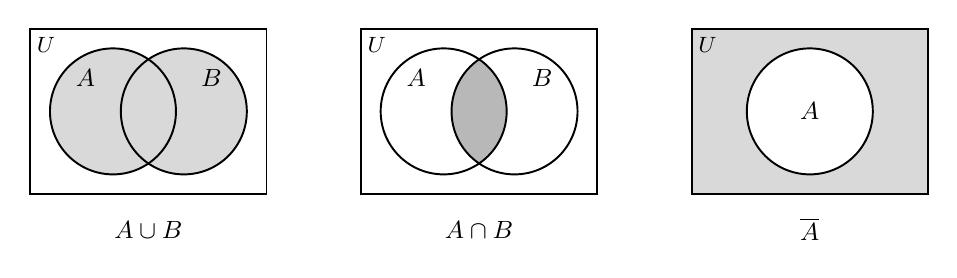
\begin{tikzpicture}[every node/.style={font=\small},line width=0.7pt]
  % all three share an identical universe rectangle U (balanced row, common baseline);
  % radius 0.8 circles in the upper-lobe label positions, consistent shading and gaps.
  % --- A union B ---
  \begin{scope}
    \fill[black!15] (-0.45,0) circle (0.8);
    \fill[black!15] (0.45,0) circle (0.8);
    \draw (-1.5,-1.05) rectangle (1.5,1.05);
    \draw (-0.45,0) circle (0.8);
    \draw (0.45,0) circle (0.8);
    \node[font=\footnotesize] at (-1.3,0.85) {$U$};
    \node at (-0.8,0.42) {$A$};
    \node at (0.8,0.42) {$B$};
    \node at (0,-1.5) {$A\cup B$};
  \end{scope}
  % --- A intersect B ---
  \begin{scope}[xshift=4.2cm]
    \begin{scope}
      \clip (-0.45,0) circle (0.8);
      \fill[black!28] (0.45,0) circle (0.8);
    \end{scope}
    \draw (-1.5,-1.05) rectangle (1.5,1.05);
    \draw (-0.45,0) circle (0.8);
    \draw (0.45,0) circle (0.8);
    \node[font=\footnotesize] at (-1.3,0.85) {$U$};
    \node at (-0.8,0.42) {$A$};
    \node at (0.8,0.42) {$B$};
    \node at (0,-1.5) {$A\cap B$};
  \end{scope}
  % --- complement of A ---
  \begin{scope}[xshift=8.4cm]
    \fill[black!15] (-1.5,-1.05) rectangle (1.5,1.05);
    \fill[white] (0,0) circle (0.8);
    \draw (-1.5,-1.05) rectangle (1.5,1.05);
    \draw (0,0) circle (0.8);
    \node[font=\footnotesize] at (-1.3,0.85) {$U$};
    \node at (0,0) {$A$};
    \node at (0,-1.5) {$\overline{A}$};
  \end{scope}
\end{tikzpicture}
\end{center}

\begin{definition}[Power set]\label{def:powerset@c1}
The \emph{power set} of $A$, written $\pow{A}$, is the set of all subsets of $A$:
$\pow{A}=\set{S\st S\subseteq A}$. If $\card{A}=n$ then $\card{\pow{A}}=2^{n}$, since each element
is independently either in or out of a subset.
\end{definition}

\begin{proposition}[De Morgan's laws]\label{prop:demorgan@c1}
For all $A,B\subseteq U$,
$\overline{A\cup B}=\overline{A}\cap\overline{B}$ and
$\overline{A\cap B}=\overline{A}\cup\overline{B}$.
\end{proposition}

\begin{proof}
We prove the first identity by mutual inclusion; the second is identical with the roles of
``and''/``or'' swapped. Take any $x\in\overline{A\cup B}$. By definition of complement, $x\notin
A\cup B$, so $x$ is in neither $A$ nor $B$; hence $x\in\overline A$ and $x\in\overline B$, that is
$x\in\overline A\cap\overline B$. This shows $\overline{A\cup B}\subseteq\overline A\cap\overline B$.
Conversely, if $x\in\overline A\cap\overline B$ then $x\notin A$ and $x\notin B$, so $x$ belongs to
neither, i.e.\ $x\notin A\cup B$, giving $x\in\overline{A\cup B}$. The two inclusions together yield
equality.
\end{proof}

\subsection*{Sequences, tuples, and the Cartesian product}

\begin{definition}[Sequence, tuple, Cartesian product]\label{def:tuple@c1}
A \emph{sequence} is an ordered list; we write it in parentheses, as $(7,1,7)$. Unlike a set, a
sequence cares about \emph{order} and \emph{repetition}, so $(1,2)\neq(2,1)$ and $(7,7)\neq(7)$. A
finite sequence of length $k$ is a \emph{$k$-tuple}; a $2$-tuple is an \emph{ordered pair}. The
\emph{Cartesian product} of sets $A_1,\dots,A_k$ is the set of all $k$-tuples with one entry from
each:
\[
  A_1\times\cdots\times A_k=\set{(a_1,\dots,a_k)\st a_i\in A_i\text{ for each }i}.
\]
We abbreviate the $k$-fold product of $A$ with itself as $A^{k}$. If each $A_i$ is finite then
$\card{A_1\times\cdots\times A_k}=\card{A_1}\cdots\card{A_k}$.
\end{definition}

\begin{wex}{Listing a Cartesian product as a grid}
With $A=\set{1,2,3}$ and $B=\set{\str a,\str b}$, list $A\times B$ and confirm its size.
\wrec The phrase ``all ordered pairs, first entry from $A$, second from $B$'' is the literal
definition of a Cartesian product, so we enumerate row by row. The trigger is the word ``pairs''
together with two named source sets.
\wsol Lay the elements of $A$ down the rows and the elements of $B$ across the columns; each cell is
one pair. There are $\card A\cdot\card B=3\cdot2=6$ cells, matching
Definition~\ref{def:tuple@c1}.
\begin{center}
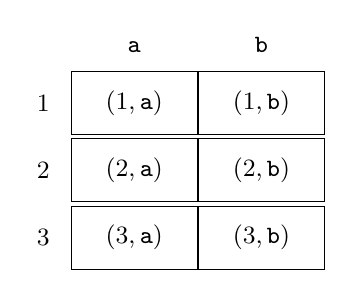
\begin{tikzpicture}[scale=0.95,every node/.style={font=\small}]
  \foreach \i/\a in {0/1,1/2,2/3} {
    \node[anchor=east] at (-0.15,-\i*0.9) {$\a$};
  }
  \foreach \j/\b in {0/{\str a},1/{\str b}} {
    \node[anchor=south] at (\j*1.7+0.85,0.55) {$\b$};
  }
  \foreach \i/\a in {0/1,1/2,2/3} {
    \foreach \j/\b in {0/{\str a},1/{\str b}} {
      \node[draw,minimum width=1.6cm,minimum height=0.8cm,inner sep=1pt]
        at (\j*1.7+0.85,-\i*0.9) {$(\a,\b)$};
    }
  }
\end{tikzpicture}
\end{center}
\whichrule{A Cartesian product is exactly a two-axis grid of pairs, so reading it off a table
guarantees we hit every combination once and the count is the product of the side lengths.}
\emph{Check.} The grid has $6$ cells and no pair is repeated, agreeing with
$\card{A\times B}=6$. Swapping to $B\times A$ would give pairs like $(\str a,1)$ -- a different set,
since order matters.
\end{wex}

\subsection*{Functions}

\begin{definition}[Function, domain, codomain, range]\label{def:function@c1}
A \emph{function} $f\colon D\to C$ assigns to \emph{each} element $x$ of its \emph{domain} $D$
exactly one element $f(x)$ of its \emph{codomain} $C$. The \emph{range} (or image) of $f$ is the set
of values actually attained, $\operatorname{ran}(f)=\set{f(x)\st x\in D}\subseteq C$. We call $f$
\begin{itemize}[leftmargin=2.2em,topsep=2pt,itemsep=1pt]
  \item \emph{injective} (one-to-one) if distinct inputs give distinct outputs:
  $x\neq y\imp f(x)\neq f(y)$;
  \item \emph{surjective} (onto) if every codomain element is hit:
  $\operatorname{ran}(f)=C$;
  \item \emph{bijective} if it is both injective and surjective.
\end{itemize}
\end{definition}

The two clauses ``each $x$ gets a value'' and ``exactly one value'' are precisely the
\emph{determinism} we will demand of a transition function later: no input is left unhandled, and
none has two answers. The picture of a function is a bundle of arrows leaving the domain dots, with
the defining property that exactly one arrow leaves each left-hand dot.

\begin{wex}{Reading injective, surjective, bijective off arrow diagrams}
Classify each of the three maps $D\to C$ below as injective, surjective, both, or neither.
\wrec The defining conditions are visual: injective means ``no two arrows land on the same
target,'' surjective means ``every target is hit,'' and bijective is both. The trigger is being
handed explicit input--output arrows, so we just inspect arrowheads.
\wsol Read each diagram against Definition~\ref{def:function@c1}.
\begin{center}
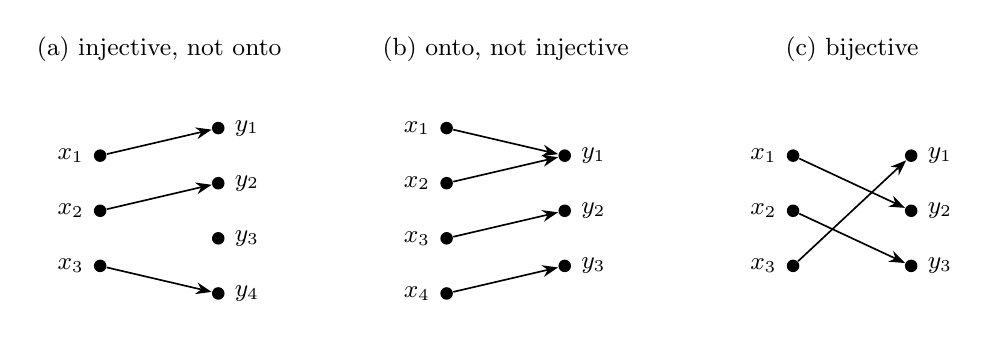
\begin{tikzpicture}[every node/.style={font=\small},
    dot/.style={circle,fill=black,inner sep=1.6pt},
    ar/.style={-{Stealth[length=2mm]},line width=0.6pt}]
  % ---- map 1: injective not surjective ----
  \begin{scope}
    \node at (0.75,1.35) {(a) injective, not onto};
    \foreach \i in {1,2,3} \node[dot,label=left:$x_{\i}$] (a\i) at (0,-\i*0.7+0.7) {};
    \foreach \i in {1,2,3,4} \node[dot,label=right:$y_{\i}$] (b\i) at (1.5,-\i*0.7+1.05) {};
    \draw[ar] (a1) -- (b1);
    \draw[ar] (a2) -- (b2);
    \draw[ar] (a3) -- (b4);
  \end{scope}
  % ---- map 2: surjective not injective ----
  \begin{scope}[xshift=4.4cm]
    \node at (0.75,1.35) {(b) onto, not injective};
    \foreach \i in {1,2,3,4} \node[dot,label=left:$x_{\i}$] (a\i) at (0,-\i*0.7+1.05) {};
    \foreach \i in {1,2,3} \node[dot,label=right:$y_{\i}$] (b\i) at (1.5,-\i*0.7+0.7) {};
    \draw[ar] (a1) -- (b1);
    \draw[ar] (a2) -- (b1);
    \draw[ar] (a3) -- (b2);
    \draw[ar] (a4) -- (b3);
  \end{scope}
  % ---- map 3: bijective ----
  \begin{scope}[xshift=8.8cm]
    \node at (0.75,1.35) {(c) bijective};
    \foreach \i in {1,2,3} \node[dot,label=left:$x_{\i}$] (a\i) at (0,-\i*0.7+0.7) {};
    \foreach \i in {1,2,3} \node[dot,label=right:$y_{\i}$] (b\i) at (1.5,-\i*0.7+0.7) {};
    \draw[ar] (a1) -- (b2);
    \draw[ar] (a2) -- (b3);
    \draw[ar] (a3) -- (b1);
  \end{scope}
\end{tikzpicture}
\end{center}
In (a) every target receives at most one arrow (injective), but $y_3$ is unhit, so it is not onto.
In (b) every target is hit (onto), but $y_1$ receives two arrows, so it is not injective. In (c)
each target receives exactly one arrow, so the map is both -- a bijection.
\whichrule{Injectivity is a statement about \emph{collisions} at the codomain (at most one arrow
per target) and surjectivity about \emph{coverage} (at least one arrow per target); a bijection
demands exactly one, which is why a bijection between finite sets forces $\card D=\card C$.}
\emph{Check.} In (c), $\card D=\card C=3$, the equality a bijection requires. In (a),
$\card D=3<4=\card C$, so onto was impossible from the start; in (b), $\card D=4>3=\card C$, so
injectivity was impossible -- the counts alone predicted both failures.
\end{wex}

\begin{wex}{A function given by a table: successor modulo $4$}
Let $f\colon \Z_4\to\Z_4$ on $\Z_4=\set{0,1,2,3}$ be $f(n)=(n+1)\bmod 4$. Tabulate $f$ and decide
whether it is a bijection.
\wrec ``Add one, then wrap'' is a complete rule for every input in a finite domain, so a finite
table captures the whole function. The trigger ``$f\colon \Z_4\to\Z_4$ with an explicit formula''
tells us to evaluate the formula at each of the four inputs.
\wsol Evaluate $(n+1)\bmod 4$ at $n=0,1,2,3$:
\begin{center}
\renewcommand{\arraystretch}{1.2}
$\begin{array}{c|cccc}
 n & 0 & 1 & 2 & 3\\\hline
 f(n) & 1 & 2 & 3 & 0
\end{array}$
\end{center}
Every output value $0,1,2,3$ appears exactly once in the bottom row. Appearing \emph{at least} once
each is surjectivity; appearing \emph{at most} once each is injectivity; both hold, so $f$ is a
bijection.
\whichrule{For a function on a \emph{finite} set to itself, injective, surjective, and bijective all
coincide -- a single missing or repeated output value would break all three at once -- so checking
that the output row is a permutation of the input row settles every case.}
\emph{Check.} The bottom row $1,2,3,0$ is a rearrangement of $0,1,2,3$, confirming the permutation.
The inverse map is $f\inv(n)=(n-1)\bmod 4$, which exists precisely because $f$ is a bijection.
\end{wex}

\subsection*{Relations and equivalence relations}

\begin{definition}[Binary relation]\label{def:relation@c1}
A \emph{binary relation} on a set $A$ is any subset $R\subseteq A\times A$. We write $x\mathrel{R}y$
to mean $(x,y)\in R$. A relation can be drawn as a \emph{directed graph}: one node per element of
$A$, and an arrow from $x$ to $y$ whenever $x\mathrel{R}y$.
\end{definition}

\begin{definition}[Reflexive, symmetric, transitive; equivalence relation]\label{def:equivrel@c1}
A binary relation $R$ on $A$ is
\begin{itemize}[leftmargin=2.2em,topsep=2pt,itemsep=1pt]
  \item \emph{reflexive} if $x\mathrel{R}x$ for every $x\in A$ (every node has a self-loop);
  \item \emph{symmetric} if $x\mathrel{R}y$ implies $y\mathrel{R}x$ (every arrow has a reverse
  arrow);
  \item \emph{transitive} if $x\mathrel{R}y$ and $y\mathrel{R}z$ imply $x\mathrel{R}z$ (every
  two-step path has a direct shortcut).
\end{itemize}
A relation that is reflexive, symmetric, and transitive is an \emph{equivalence relation}.
\end{definition}

\begin{wex}{Spotting which of the three properties fail}
On $A=\set{1,2,3}$ let $R=\set{(1,1),(2,2),(3,3),(1,2),(2,1),(2,3)}$. Draw its directed graph and
determine which of reflexivity, symmetry, transitivity hold.
\wrec The three properties are graph-shaped: self-loops (reflexive), paired arrows (symmetric),
and shortcut arrows for two-step paths (transitive). The trigger is an explicitly listed relation,
so we plot the arrows and look.
\wsol Plot a node per element and an arrow per listed pair. Self-loops at $1,2,3$ come from
$(1,1),(2,2),(3,3)$; the double arrow $1\leftrightarrow2$ comes from $(1,2)$ and $(2,1)$; and a lone
arrow $2\to3$ comes from $(2,3)$.
\begin{center}
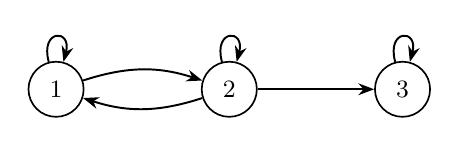
\begin{tikzpicture}[every node/.style={font=\small},
    rv/.style={circle,draw=black,line width=0.6pt,minimum size=7mm,inner sep=0.5pt},
    re/.style={-{Stealth[length=2mm]},line width=0.7pt}]
  \node[rv] (n1) at (0,0) {$1$};
  \node[rv] (n2) at (2.2,0) {$2$};
  \node[rv] (n3) at (4.4,0) {$3$};
  \draw[re] (n1) edge[loop above,looseness=6] (n1);
  \draw[re] (n2) edge[loop above,looseness=6] (n2);
  \draw[re] (n3) edge[loop above,looseness=6] (n3);
  \draw[re] (n1) edge[bend left=18] (n2);
  \draw[re] (n2) edge[bend left=18] (n1);
  \draw[re] (n2) -- (n3);
\end{tikzpicture}
\end{center}
\emph{Reflexive:} yes -- every node carries a self-loop. \emph{Symmetric:} no -- there is an arrow
$2\to3$ but none $3\to2$. \emph{Transitive:} no -- $1\mathrel{R}2$ and $2\mathrel{R}3$ hold, yet the
shortcut $1\mathrel{R}3$ is missing. So $R$ is reflexive only, and is \emph{not} an equivalence
relation.
\whichrule{Each property is a closure demand on the graph -- a missing self-loop, a missing reverse
arrow, or a missing shortcut breaks the corresponding property -- so a single counterexample edge
settles the question, no exhaustive search needed.}
\emph{Check.} Adding $(3,2)$ would restore symmetry, but transitivity would still need $(1,3)$ and
$(3,1)$; only when all such forced edges are present does the graph become an equivalence relation,
splitting $A$ into one block $\set{1,2,3}$.
\end{wex}

\begin{definition}[Equivalence class, partition]\label{def:partition@c1}
Let $R$ be an equivalence relation on $A$. The \emph{equivalence class} of $x$ is
$[x]=\set{y\in A\st x\mathrel{R}y}$. A \emph{partition} of $A$ is a collection of nonempty, pairwise
disjoint subsets (\emph{blocks}) whose union is $A$.
\end{definition}

\begin{theorem}[Equivalence relations and partitions correspond]\label{thm:partition@c1}
Let $R$ be an equivalence relation on $A$. Then the distinct equivalence classes of $R$ form a
partition of $A$. Conversely, every partition of $A$ arises from exactly one equivalence relation,
namely ``$x$ and $y$ lie in the same block.''
\end{theorem}

\begin{proof}
First we show the classes partition $A$. Each class is nonempty, since $x\in[x]$ by reflexivity, and
their union is all of $A$ because every $x$ lies in its own class. It remains to show distinct
classes are disjoint; equivalently, that if $[x]\cap[y]\neq\es$ then $[x]=[y]$. Suppose
$z\in[x]\cap[y]$, so $x\mathrel{R}z$ and $y\mathrel{R}z$. By symmetry $z\mathrel{R}y$, and by
transitivity $x\mathrel{R}y$. Now take any $w\in[x]$, so $x\mathrel{R}w$; symmetry gives
$w\mathrel{R}x$, and combined with $x\mathrel{R}y$ transitivity gives $w\mathrel{R}y$, i.e.\ (using
symmetry again) $y\mathrel{R}w$, so $w\in[y]$. Thus $[x]\subseteq[y]$, and the symmetric argument
gives $[y]\subseteq[x]$, hence $[x]=[y]$.

Conversely, given a partition, define $x\sim y$ to mean ``$x$ and $y$ are in the same block.'' This
relation is reflexive ($x$ shares its block with itself), symmetric (``same block'' does not depend
on order), and transitive (if $x,y$ share a block and $y,z$ share a block, then since blocks are
disjoint these are the same block, so $x,z$ share it). Its classes are exactly the blocks, and no
other equivalence relation yields the same blocks, since the relation is forced by them.
\end{proof}

\begin{wex}{The classes of congruence modulo $3$ partition $\Z$}
Define $x\equiv y$ to mean $3\mid(x-y)$ on the integers $\Z$. Verify it is an equivalence relation
and exhibit its partition.
\wrec ``Differ by a multiple of $3$'' has the algebraic shape of a congruence, and congruences are
the classic source of equivalence relations. The trigger ``$x-y$ is divisible by a fixed $m$''
points straight at reflexive/symmetric/transitive via simple divisibility facts.
\wsol \emph{Reflexive:} $x-x=0=3\cdot0$, divisible by $3$. \emph{Symmetric:} if $x-y=3k$ then
$y-x=3(-k)$. \emph{Transitive:} if $x-y=3k$ and $y-z=3\ell$ then $x-z=3(k+\ell)$. So $\equiv$ is an
equivalence relation. By Theorem~\ref{thm:partition@c1} its classes partition $\Z$, and the class of
$x$ is determined by the remainder of $x$ on division by $3$, giving three blocks. We picture them as
three disjoint cells covering $\Z$.
\begin{center}
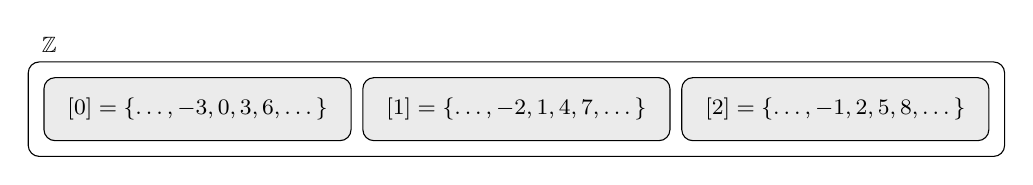
\begin{tikzpicture}[every node/.style={font=\footnotesize}]
  \draw[rounded corners] (-0.15,-0.15) rectangle (12.25,1.05);
  \node[anchor=south west,font=\footnotesize] at (-0.1,1.05) {$\Z$};
  \foreach \k/\lbl/\xs in {0/{$[0]=\set{\dots,-3,0,3,6,\dots}$}/0,
                           1/{$[1]=\set{\dots,-2,1,4,7,\dots}$}/4.05,
                           2/{$[2]=\set{\dots,-1,2,5,8,\dots}$}/8.1} {
    \draw[fill=black!8,rounded corners] (\xs+0.05,0.05) rectangle (\xs+3.95,0.85);
    \node at (\xs+2.0,0.45) {\lbl};
  }
\end{tikzpicture}
\end{center}
\whichrule{Congruence modulo $m$ is an equivalence relation whose classes are the $m$ residue
classes; this is the very mechanism a counting-mod-$m$ automaton will exploit later, where each
class becomes one state.}
\emph{Check.} The three blocks are nonempty, pairwise disjoint, and every integer lands in exactly
one according to its remainder mod $3$ -- the defining conditions of a partition. There are exactly
$\card{\Z_3}=3$ classes, as expected.
\end{wex}

\subsection*{Ordering subsets: a Hasse diagram}

Not every useful relation is an equivalence relation. The subset relation $\subseteq$ on a power set
is reflexive and transitive but \emph{antisymmetric} (if $A\subseteq B$ and $B\subseteq A$ then
$A=B$), making it a \emph{partial order}. We can draw a partial order compactly with a \emph{Hasse
diagram}: place smaller sets lower, larger sets higher, and draw an edge only for a \emph{covering}
step (one set immediately above another with nothing strictly between). The next example shows the
power set of a three-element set, the same $2^{3}=8$ subsets counted in
Definition~\ref{def:powerset@c1}.

\begin{wex}{The Boolean lattice on $\set{a,b,c}$}
Draw the Hasse diagram of $\bigl(\pow{\set{a,b,c}},\subseteq\bigr)$.
\wrec The objects are the subsets of a $3$-element set ordered by inclusion; ``ordered by
inclusion, draw only covers'' is the recipe for a Hasse diagram. The trigger is a partial order
(reflexive, antisymmetric, transitive) on a small finite set.
\wsol List the $8$ subsets by size: one empty set at the bottom, three singletons, three pairs, and
the full set at the top. An edge joins $S$ to $T$ exactly when $T=S\cup\set{x}$ for a single new
element $x$ -- a one-element growth step. This stacks into four levels.
\begin{center}
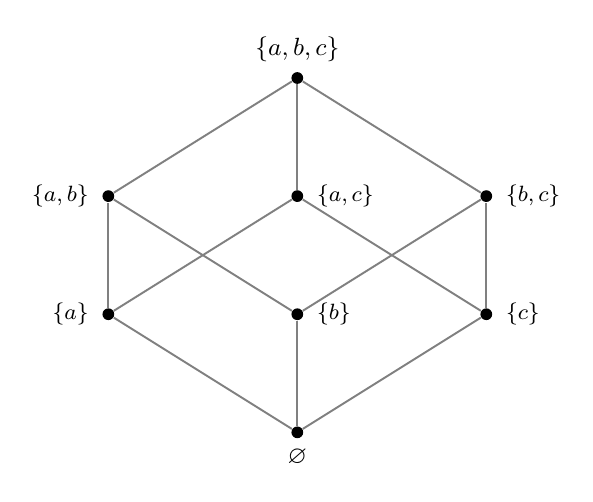
\begin{tikzpicture}[every node/.style={font=\small}]
  % level 0
  \node[ltdot,label=below:{$\es$}] (e) at (0,0) {};
  % level 1: singletons
  \node[ltdot] (a) at (-2.4,1.5) {};  \node[ltlab,left=3pt of a] {$\set{a}$};
  \node[ltdot] (b) at (0,1.5) {};     \node[ltlab,right=3pt of b] {$\set{b}$};
  \node[ltdot] (c) at (2.4,1.5) {};   \node[ltlab,right=3pt of c] {$\set{c}$};
  % level 2: pairs
  \node[ltdot] (ab) at (-2.4,3.0) {}; \node[ltlab,left=3pt of ab] {$\set{a,b}$};
  \node[ltdot] (ac) at (0,3.0) {};    \node[ltlab,right=3pt of ac] {$\set{a,c}$};
  \node[ltdot] (bc) at (2.4,3.0) {};  \node[ltlab,right=3pt of bc] {$\set{b,c}$};
  % level 3: full
  \node[ltdot,label=above:{$\set{a,b,c}$}] (f) at (0,4.5) {};
  % covering edges
  \draw[ltedge] (e)--(a); \draw[ltedge] (e)--(b); \draw[ltedge] (e)--(c);
  \draw[ltedge] (a)--(ab); \draw[ltedge] (a)--(ac);
  \draw[ltedge] (b)--(ab); \draw[ltedge] (b)--(bc);
  \draw[ltedge] (c)--(ac); \draw[ltedge] (c)--(bc);
  \draw[ltedge] (ab)--(f); \draw[ltedge] (ac)--(f); \draw[ltedge] (bc)--(f);
\end{tikzpicture}
\end{center}
\whichrule{For a finite partial order, a Hasse diagram shows \emph{only} covering edges; all other
comparabilities (such as $\es\subseteq\set{a,b}$) are recovered as upward paths, which keeps the
picture readable while losing no information.}
\emph{Check.} The diagram has $8$ nodes ($=2^{3}$, agreeing with $\card{\pow{\set{a,b,c}}}$) and is
symmetric top-to-bottom: complementation $S\mapsto\overline S$ flips the picture upside down, sending
each level $k$ to level $3-k$.
\end{wex}

\begin{method}{How to read or build a function/relation diagram}
\begin{enumerate}[leftmargin=2em,topsep=2pt,itemsep=1pt]
  \item \textbf{Identify the kind of object.} A \emph{function} $D\to C$ is one arrow out of every
  domain dot; a \emph{relation} on $A$ is any set of arrows among $A$'s dots. If you ever see a
  domain dot with zero or two outgoing arrows, it is not a function.
  \item \textbf{For functions, test the two failure modes separately.} Injective fails iff two
  arrows share a target; surjective fails iff some codomain dot has no incoming arrow. Bijective
  means neither failure occurs.
  \item \textbf{For relations, translate each property to a shape.} Reflexive $=$ every dot has a
  self-loop; symmetric $=$ every arrow is matched by its reverse; transitive $=$ every length-two
  path has its shortcut. To disprove a property, exhibit one missing edge.
  \item \textbf{If it is an equivalence relation, read off the partition.} The connected blocks of
  mutually related elements are the equivalence classes; check they are nonempty, disjoint, and
  cover $A$.
  \item \textbf{If it is a partial order, draw the Hasse diagram.} Put minimal elements at the
  bottom, draw only covering edges, and recover all other comparabilities as upward paths.
\end{enumerate}
\end{method}

\begin{pitfall}
Do not conflate the \emph{codomain} $C$ with the \emph{range} $\operatorname{ran}(f)$. The codomain
is declared in advance as part of the function's type $f\colon D\to C$; the range is whatever values
$f$ actually produces. Surjectivity is precisely the statement that these two coincide. The same map
can be onto one codomain and not onto a larger one, so ``surjective'' is only meaningful once the
codomain is fixed.
\end{pitfall}

\begin{pitfall}
``Symmetric'' and ``antisymmetric'' are not opposites, and a relation can be neither. Symmetry says
every arrow has a reverse; antisymmetry says no two \emph{distinct} elements have arrows both ways
(self-loops are still allowed). The relation $\set{(1,2),(2,1),(2,3)}$ is neither symmetric (no reverse
of $2\to3$) nor antisymmetric ($1\to2$ and $2\to1$), while $\set{(1,2),(2,1)}$ is symmetric but not
antisymmetric.
Equivalence relations are built from symmetry; partial orders are built from antisymmetry -- mixing
the two is a frequent slip when classifying a relation.
\end{pitfall}

\begin{pitfall}
The empty set $\es$ is a subset of \emph{every} set, and it is an \emph{element} of a power set, not
the same thing as ``no set at all.'' In particular $\es\in\pow{A}$ always, so $\pow{A}$ is never
empty even when $A=\es$: indeed $\pow{\es}=\set{\es}$ has one element, not zero. Confusing $\es$ (a
set with no members) with $\set{\es}$ (a set whose single member is the empty set) is a classic
error that also breaks the count $\card{\pow{A}}=2^{\card A}$ at $\card A=0$.
\end{pitfall}

\begin{exers}{Exercises.}
\item Let $A=\set{1,2,3,4}$, $B=\set{3,4,5}$, with universe $U=\set{1,2,3,4,5,6}$. Compute
$A\cup B$, $A\cap B$, $A\setminus B$, $B\setminus A$, $\overline{A}$, and $\overline{A\cup B}$. Then
verify $\overline{A\cup B}=\overline{A}\cap\overline{B}$ directly from your lists.

\item Let $A=\set{\str x,\str y}$ and $B=\set{1,2,3}$. List $A\times B$ and $B\times A$ explicitly,
confirm both have $\card A\cdot\card B$ pairs, and explain in one sentence why $A\times B\neq B\times
A$ as sets even though they have the same size. Draw the $A\times B$ grid.

\item List the power set $\pow{\set{p,q,r}}$ in full, grouped by size, and check that it has $2^{3}$
members. Which of these eight subsets are subsets of $\set{p,q}$?

\item For a set $A$ with $\card A=n$, prove that $\card{\pow{A}}=2^{n}$ by describing a bijection
between subsets of $A$ and length-$n$ strings over $\set{0,1}$ (the ``indicator string'' of a subset).
Draw the arrow diagram of this bijection for $n=2$, i.e.\ between $\pow{\set{a,b}}$ and
$\set{0,1}^{2}$.

\item Define $f\colon\set{0,1,2,3,4}\to\set{0,1,2,3,4}$ by $f(n)=(2n)\bmod 5$. Tabulate $f$, draw its
arrow diagram, and decide whether it is injective, surjective, bijective. If it is a bijection, give
$f\inv$ as a table.

\item Give an explicit example of each, as an arrow diagram between small finite sets, or argue that
none exists: (a) a function that is injective but not surjective; (b) one that is surjective but not
injective; (c) a function $g\colon A\to A$ on a \emph{finite} set $A$ that is injective but not
surjective. (For (c), state precisely why your answer is forced.)

\item Let $A=\set{1,2,3}$. Decide for each of the following relations on $A$ which of reflexive,
symmetric, transitive hold, drawing the directed graph of each: (a) $R_1=\set{(1,1),(2,2),(3,3)}$;
(b) $R_2=\set{(1,2),(2,1),(1,1),(2,2)}$; (c) $R_3=\set{(1,2),(2,3),(1,3)}$. Which, if any, are
equivalence relations, and what partition does each equivalence relation induce?

\item On the set $L=\set{\str a,\str{ab},\str{abc},\str b,\str{bc},\str c}$ of strings, define
$x\preceq y$ to mean ``$x$ is a prefix of $y$.'' Argue that $\preceq$ is a partial order (reflexive,
antisymmetric, transitive) and draw its Hasse diagram.

\item Define a relation $\sim$ on $\set{0,1}\kstar$ by $x\sim y$ iff $x$ and $y$ have the same length.
Prove $\sim$ is an equivalence relation, describe its equivalence classes, and say how many strings
are in the class of a string of length $n$. (This ``same length'' partition reappears when we count
strings in the next section.)

\item Let $f\colon A\to B$ be a function and let $S,T\subseteq A$. Prove that $f(S\cup T)=f(S)\cup
f(T)$. Then show by a concrete two-point counterexample that $f(S\cap T)=f(S)\cap f(T)$ can
\emph{fail}, and identify which property of $f$ (if assumed) would make it always hold.

\item \emph{Find the bug.} A student writes: ``The relation $R=\set{(1,1),(2,2),(1,2)}$ on
$\set{1,2}$ is an equivalence relation because it is reflexive and transitive.'' Draw the graph,
state precisely which axiom fails, give the single pair that must be added to repair it, and name the
partition of $\set{1,2}$ that the repaired relation induces.

\item \emph{Find the bug.} Someone argues: ``Every relation that is symmetric and transitive is also
reflexive: take any $x$, pick some $y$ with $x\mathrel{R}y$, then symmetry gives $y\mathrel{R}x$ and
transitivity gives $x\mathrel{R}x$.'' Exhibit a symmetric, transitive relation that is \emph{not}
reflexive, and pinpoint the exact unjustified step in the argument.
\end{exers}


\section{Strings, Alphabets, and Languages}
Everything a machine in this book reads, writes, or decides about is a \emph{string}, and every
problem we study is ultimately a \emph{language} -- a set of strings. This section pins down those two
objects and the handful of operations on them (length, concatenation, reversal, the prefix and
substring relations, and the language operations union, concatenation, and star). The one key idea is
that strings are built by a single operation, concatenation, with the empty string $\eps$ as its
neutral element; once that is clear, every later definition -- regular expressions, the moves of an
automaton, the contents of a Turing tape -- is just structured talk about concatenation. We build up
from a single symbol to alphabets, to strings, and finally to languages, computing small examples at
each step.

\begin{definition}[Alphabet and symbol]\label{def:alphabet@c1}
An \emph{alphabet} is any nonempty finite set $\Sig$. Its elements are called \emph{symbols}. We write
symbols in a typewriter font, e.g.\ $\str0,\str1,\str a,\str b$.
\end{definition}

The two alphabets we use most are the binary alphabet $\Sig=\set{\str0,\str1}$ and small letter
alphabets such as $\set{\str a,\str b}$. Finiteness and nonemptiness are both essential: a machine with
infinitely many distinct input symbols could not be described in finite space, and an empty alphabet
admits no nonempty input at all.

\begin{definition}[String and its length]\label{def:string@c1}
A \emph{string} over $\Sig$ is a finite sequence of symbols from $\Sig$, written by juxtaposition with
no separators. If $w=w_1w_2\cdots w_n$ with each $w_i\in\Sig$, the \emph{length} of $w$ is
$\abs{w}=n$, the number of symbol occurrences. The unique string of length $0$ is the \emph{empty
string} $\eps$. We write $\Sigstar$ for the set of \emph{all} strings over $\Sig$, and $\Sig^{n}$ for
the set of strings of length exactly $n$, so that $\Sig^{0}=\set{\eps}$.
\end{definition}

A string is a sequence, so order and repetition both matter: over $\set{\str a,\str b}$ the strings
$\str{ab}$ and $\str{ba}$ are different, and $\str{aa}$ differs from $\str a$. This is exactly the
opposite of a set, where $\set{\str a,\str b}=\set{\str b,\str a}$ and $\set{\str a,\str a}=\set{\str
a}$. Picture a string as a row of labelled cells, one per symbol occurrence, read left to right.

\begin{center}
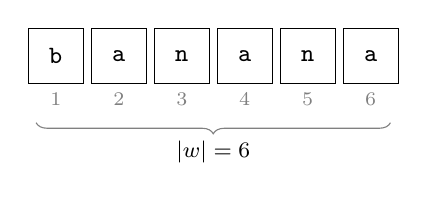
\begin{tikzpicture}[every node/.style={font=\small}]
  \foreach \i/\c in {1/\str b,2/\str a,3/\str n,4/\str a,5/\str n,6/\str a}{
    \node[draw,minimum size=7mm,inner sep=1pt] (c\i) at (\i*0.8,0) {$\c$};
    \node[font=\scriptsize,gray] at (\i*0.8,-0.55) {\i};
  }
  \draw[decorate,decoration={brace,amplitude=4pt,mirror},gray]
        (0.55,-0.85) -- (5.05,-0.85) node[midway,below=3pt,black,font=\footnotesize]
        {$\abs{w}=6$};
\end{tikzpicture}
\end{center}

The numbers under the cells stress that length counts \emph{positions}, not \emph{distinct symbols}:
the string $\str{banana}$ above has length $6$ even though only three symbols ($\str b,\str a,\str n$)
appear in it.

\begin{definition}[Concatenation]\label{def:concat@c1}
If $x=x_1\cdots x_m$ and $y=y_1\cdots y_n$ are strings over $\Sig$, their \emph{concatenation} is
$xy=x_1\cdots x_m y_1\cdots y_n$, the string formed by writing $x$ and then $y$. We sometimes write it
$x\concat y$ when juxtaposition would be ambiguous. The \emph{$k$-fold power} of $x$ is
$x^0=\eps$ and $x^{k}=x^{k-1}x$ for $k\ge 1$.
\end{definition}

\begin{proposition}[Concatenation is a monoid operation]\label{prop:monoid@c1}
For all strings $x,y,z\in\Sigstar$,
\[
  (xy)z=x(yz),\qquad \eps x=x\eps=x,\qquad \abs{xy}=\abs{x}+\abs{y}.
\]
\end{proposition}

\begin{proof}
Write $x=x_1\cdots x_m$, $y=y_1\cdots y_n$, $z=z_1\cdots z_p$. Both $(xy)z$ and $x(yz)$ are, by
Definition~\ref{def:concat@c1} applied twice, the single sequence
$x_1\cdots x_m\,y_1\cdots y_n\,z_1\cdots z_p$ of length $m+n+p$; juxtaposition records no grouping, so
the two are literally the same string. Prepending or appending the length-$0$ sequence $\eps$ adds no
positions, giving $\eps x=x\eps=x$. Finally $xy$ lists the $m$ positions of $x$ followed by the $n$
positions of $y$, so it has $m+n$ positions, i.e.\ $\abs{xy}=\abs{x}+\abs{y}$.
\end{proof}

So $\Sigstar$ with concatenation is a monoid: an associative operation with identity $\eps$. It is
\emph{not} commutative once $\abs{\Sig}\ge 2$ ($\str{ab}\ne\str{ba}$), which is why ``concatenation
order'' is something to watch. The length map $w\mapsto\abs{w}$ turns concatenation into addition --
this is the workhorse identity behind almost every length argument later.

\begin{definition}[Reversal]\label{def:rev@c1}
The \emph{reversal} of $w=w_1w_2\cdots w_n$ is $\rev{w}=w_n\cdots w_2 w_1$, the same symbols in the
opposite order. In particular $\rev{\eps}=\eps$.
\end{definition}

\begin{proposition}[Reversal flips a concatenation]\label{prop:revconcat@c1}
For all $x,y\in\Sigstar$, $\rev{(xy)}=\rev{y}\,\rev{x}$.
\end{proposition}

\begin{proof}
Let $x=x_1\cdots x_m$ and $y=y_1\cdots y_n$. Then $xy=x_1\cdots x_m y_1\cdots y_n$, and reversing this
length-$(m+n)$ sequence reads its symbols from the last position to the first:
$y_n\cdots y_1\,x_m\cdots x_1$. The first block $y_n\cdots y_1$ is $\rev{y}$ and the second block
$x_m\cdots x_1$ is $\rev{x}$, so the whole is $\rev{y}\,\rev{x}$.
\end{proof}

\begin{definition}[Prefix, suffix, substring]\label{def:substr@c1}
Let $w\in\Sigstar$. A string $x$ is a \emph{prefix} of $w$ if $w=xz$ for some $z\in\Sigstar$; it is a
\emph{suffix} if $w=zx$ for some $z$; and it is a \emph{substring} (or factor) if $w=uxv$ for some
$u,v\in\Sigstar$. A prefix (suffix, substring) is \emph{proper} if it is not equal to $w$ itself. We
write $x\substr w$ when $x$ is a substring of $w$.
\end{definition}

Every prefix and every suffix is a substring, but not conversely; and $\eps$ together with $w$ are
always among the (improper-or-proper) prefixes, suffixes, and substrings of $w$. We now compute with
all of these.

\begin{wex}{Length, powers, and reversal on a concrete string}
Let $\Sig=\set{\str a,\str b}$ and $w=\str{abb}$. Compute $\abs{w}$, $w^{2}$, $w^{0}$, $\rev{w}$, and
$\rev{(w^2)}$, and check $\rev{(w^2)}=(\rev{w})^{2}$ against Proposition~\ref{prop:revconcat@c1}.
\wrec Each quantity is a \emph{direct application} of a definition: length counts positions
(Def.~\ref{def:string@c1}), a power is repeated concatenation (Def.~\ref{def:concat@c1}), reversal flips the
order (Def.~\ref{def:rev@c1}). The trigger ``evaluate these on a specific string'' means: expand by the
definitions and read off the answer.
\wsol $\abs{w}=3$ since $w$ has three positions. The powers are $w^{0}=\eps$ and
$w^{2}=ww=\str{abb}\,\str{abb}=\str{abbabb}$, of length $6=\abs{w}+\abs{w}$, matching
Proposition~\ref{prop:monoid@c1}. Reversal: $\rev{w}=\str{bba}$. For $\rev{(w^2)}$ either reverse
$\str{abbabb}$ directly to get $\str{bbabba}$, or use Proposition~\ref{prop:revconcat@c1}:
$\rev{(ww)}=\rev{w}\,\rev{w}=\str{bba}\,\str{bba}=\str{bbabba}$.
\begin{center}
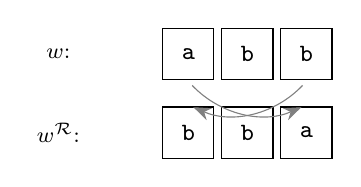
\begin{tikzpicture}[every node/.style={font=\small}]
  \node[font=\footnotesize] at (-0.9,0) {$w$:};
  \foreach \i/\c in {1/\str a,2/\str b,3/\str b}
    \node[draw,minimum size=6.5mm,inner sep=1pt] at (\i*0.75,0) {$\c$};
  \node[font=\footnotesize] at (-0.9,-1) {$\rev{w}$:};
  \foreach \i/\c in {1/\str b,2/\str b,3/\str a}
    \node[draw,minimum size=6.5mm,inner sep=1pt] at (\i*0.75,-1) {$\c$};
  \draw[->,gray,shorten >=2pt,shorten <=2pt] (0.75,-0.35) to[bend right=35] (2.25,-0.65);
  \draw[->,gray,shorten >=2pt,shorten <=2pt] (2.25,-0.35) to[bend left=35] (0.75,-0.65);
\end{tikzpicture}
\end{center}
\whichrule{Reversal of a concatenation reverses the \emph{pieces} and swaps their order
(Prop.~\ref{prop:revconcat@c1}); on a single repeated block $w$ the swap is invisible, so
$\rev{(w^k)}=(\rev{w})^{k}$.}
\emph{Check.} Both routes give $\str{bbabba}$, and indeed $(\rev{w})^2=\str{bba}\,\str{bba}=
\str{bbabba}$, confirming the identity.
\end{wex}

\begin{wex}{Listing prefixes, suffixes, and substrings; a substring poset}
For $w=\str{aba}$ over $\set{\str a,\str b}$, list all prefixes, all suffixes, and all substrings, and
draw the substrings ordered by the substring relation $\substr$.
\wrec This is a \emph{decomposition} task: a prefix is what sits to the left of a cut, a suffix what
sits to the right, a substring any contiguous window (Def.~\ref{def:substr@c1}). The trigger ``list all''
means slide a window over the positions and collect what you see, remembering that $\eps$ (the empty
window) always qualifies.
\wsol Cutting $\str{aba}$ after position $0,1,2,3$ gives the prefixes
$\eps,\str a,\str{ab},\str{aba}$. The parts to the right of the same cuts are the suffixes
$\str{aba},\str{ba},\str a,\eps$. The substrings are all contiguous windows: the empty window $\eps$;
length-$1$ windows $\str a,\str b$; length-$2$ windows $\str{ab},\str{ba}$; and the whole string
$\str{aba}$. Note $\str a$ occurs at two positions but is listed once -- substrings form a \emph{set}.
Order them by ``is a substring of'':
\begin{center}
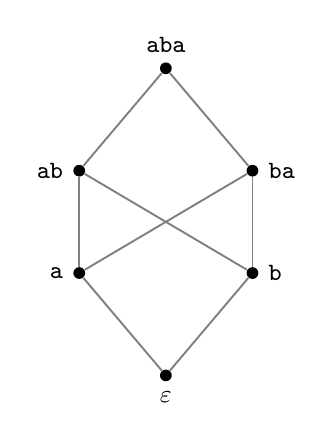
\begin{tikzpicture}[every node/.style={font=\small}]
  \node[ltdot,label=below:{$\eps$}] (e) at (0,0) {};
  \node[ltdot,label=left:{$\str a$}] (a) at (-1.1,1.3) {};
  \node[ltdot,label=right:{$\str b$}] (b) at (1.1,1.3) {};
  \node[ltdot,label=left:{$\str{ab}$}] (ab) at (-1.1,2.6) {};
  \node[ltdot,label=right:{$\str{ba}$}] (ba) at (1.1,2.6) {};
  \node[ltdot,label=above:{$\str{aba}$}] (aba) at (0,3.9) {};
  \draw[ltedge] (e)--(a); \draw[ltedge] (e)--(b);
  \draw[ltedge] (a)--(ab); \draw[ltedge] (b)--(ab);
  \draw[ltedge] (a)--(ba); \draw[ltedge] (b)--(ba);
  \draw[ltedge] (ab)--(aba); \draw[ltedge] (ba)--(aba);
\end{tikzpicture}
\end{center}
\whichrule{Prefixes and suffixes come from the $\abs{w}+1$ cut points; substrings come from all
contiguous windows. The substring relation is a partial order (reflexive, antisymmetric, transitive),
so the substrings of a fixed word form the Hasse diagram drawn above.}
\emph{Check.} There are $4$ prefixes and $4$ suffixes (always $\abs{w}+1$ of each), and the six
substrings sit in the poset with $\eps$ at the bottom (a substring of everything) and $\str{aba}$ at
the top.
\end{wex}

\textbf{From strings to languages.} A \emph{language} is any set of strings over a fixed alphabet. The
language is the thing a machine ``decides'': membership in it is the yes/no question we ask of an
input. Because languages are just sets, the ordinary set operations apply -- but there are also two
genuinely string-flavoured operations, \emph{concatenation} and \emph{star}, that have no analogue for
plain sets.

\begin{definition}[Language]\label{def:language@c1}
A \emph{language} over $\Sig$ is a subset $\Lang\subseteq\Sigstar$. The two extreme languages are the
\emph{empty language} $\es$ (no strings at all) and $\Sigstar$ itself (every string). The
singleton-empty-string language $\set{\eps}$ is a third, distinct, special case.
\end{definition}

\begin{pitfall}
Keep $\es$, $\set{\eps}$, and $\eps$ apart. They are three different things: $\es$ is a \emph{language}
with zero members; $\set{\eps}$ is a \emph{language} with exactly one member, the empty string; and
$\eps$ is a \emph{string}, not a language at all. We have $\abs{\es}=0$ and $\card{\set{\eps}}=1$ as
language sizes, while $\abs{\eps}=0$ as a string length.
\end{pitfall}

\begin{definition}[Operations on languages]\label{def:langops@c1}
Let $A,B\subseteq\Sigstar$ be languages. Their
\emph{union} $A\cup B=\set{w\st w\in A\text{ or }w\in B}$,
\emph{intersection} $A\cap B=\set{w\st w\in A\text{ and }w\in B}$, and
\emph{complement} $\overline{A}=\Sigstar\setminus A$ are the usual set operations. The string-aware
operations are:
\begin{itemize}[leftmargin=2.2em,topsep=2pt,itemsep=1pt]
  \item \emph{concatenation} $A\concat B=\set{xy\st x\in A,\ y\in B}$ (every left piece glued to every
  right piece);
  \item \emph{star} $A\kstar=\set{x_1x_2\cdots x_k\st k\ge 0,\ \text{each }x_i\in A}$, all finite
  concatenations of members of $A$, \emph{including} the empty concatenation ($k=0$), which is $\eps$;
  \item \emph{plus} $A\kplus=\set{x_1\cdots x_k\st k\ge 1,\ \text{each }x_i\in A}$, the same but with
  $k\ge 1$;
  \item \emph{reversal} $\rev{A}=\set{\rev{w}\st w\in A}$.
\end{itemize}
\end{definition}

Two relations to remember: $A\kstar=A\kplus\cup\set{\eps}$ always, and $A\kplus=A\kstar$ exactly when
$\eps\in A$. Setting $A=\Sig$ (the alphabet read as the language of its one-symbol strings) recovers
the notation $\Sigstar$ from Definition~\ref{def:string@c1}: $\Sigstar$ really is the star of the
alphabet.

\begin{wex}{Computing a concatenation of two finite languages}
Let $A=\set{\eps,\str a}$ and $B=\set{\str b,\str{bb}}$ over $\set{\str a,\str b}$. Compute $A\concat
B$, then $B\concat A$, and observe that they differ.
\wrec Concatenation of languages is a \emph{Cartesian-style pairing} (Def.~\ref{def:langops@c1}): form
every $xy$ with $x\in A$ and $y\in B$. The trigger ``concatenate two finite languages'' means take all
$\card A\cdot\card B$ glued pairs and then \emph{deduplicate}, since the result is a set.
\wsol Glue each $x\in A$ to each $y\in B$:
\begin{center}
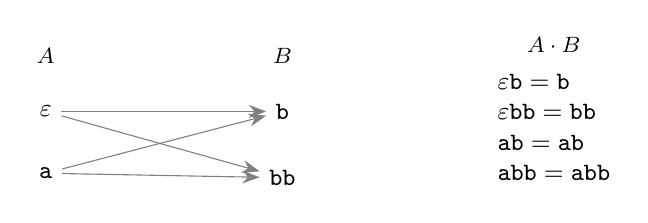
\begin{tikzpicture}[every node/.style={font=\small},node distance=8mm]
  \node (a1) {$\eps$};
  \node[below=4mm of a1] (a2) {$\str a$};
  \node[right=26mm of a1] (b1) {$\str b$};
  \node[below=4mm of b1] (b2) {$\str{bb}$};
  \node[font=\footnotesize] at ($(a1)+(0,0.7)$) {$A$};
  \node[font=\footnotesize] at ($(b1)+(0,0.7)$) {$B$};
  \node[right=24mm of b1,yshift=-2mm,align=left] (out)
    {$\eps\str b=\str b$\\ $\eps\str{bb}=\str{bb}$\\ $\str a\str b=\str{ab}$\\
     $\str a\str{bb}=\str{abb}$};
  \node[font=\footnotesize] at ($(out.north)+(0,0.25)$) {$A\concat B$};
  \draw[->,gray] (a1)--(b1); \draw[->,gray] (a1)--(b2);
  \draw[->,gray] (a2)--(b1); \draw[->,gray] (a2)--(b2);
\end{tikzpicture}
\end{center}
So $A\concat B=\set{\str b,\str{bb},\str{ab},\str{abb}}$. Going the other way,
$B\concat A=\set{\str b\eps,\str b\str a,\str{bb}\eps,\str{bb}\str a}
=\set{\str b,\str{ba},\str{bb},\str{bba}}$.
\whichrule{Language concatenation pairs \emph{every} left string with \emph{every} right string;
because string concatenation is non-commutative, $A\concat B\ne B\concat A$ in general -- here
$\str{ab}\in A\concat B$ but $\str{ab}\notin B\concat A$.}
\emph{Check.} $\card{A\concat B}=4=\card A\cdot\card B$ with no collisions; $A\concat B$ and $B\concat
A$ share only $\set{\str b,\str{bb}}$, confirming order matters.
\end{wex}

\begin{wex}{When the product count drops: collisions in concatenation}
Let $A=\set{\str a,\str{aa}}$ and $B=\set{\str a,\str{aa}}$ (so $B=A$). Compute $A\concat A$ and
explain why $\card{A\concat A}<\card A\cdot\card A$.
\wrec Same operation as before, but now the alphabet is a single letter, so different gluings can
produce the \emph{same} string -- a \emph{collision}. The trigger ``count is smaller than the product''
flags that the set quotient removes duplicates.
\wsol The four gluings are $\str a\concat\str a=\str{aa}$, $\str a\concat\str{aa}=\str{aaa}$,
$\str{aa}\concat\str a=\str{aaa}$, $\str{aa}\concat\str{aa}=\str{aaaa}$. The middle two both equal $\str{aaa}$, so
\[
  A\concat A=\set{\str{aa},\ \str{aaa},\ \str{aaaa}},\qquad \card{A\concat A}=3.
\]
\begin{center}
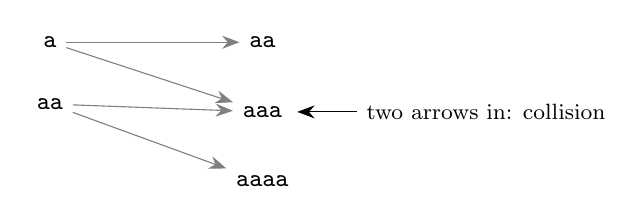
\begin{tikzpicture}[every node/.style={font=\small},node distance=7mm]
  \node (a1) {$\str a$};
  \node[below=4mm of a1] (a2) {$\str{aa}$};
  \node[right=22mm of a1] (o1) {$\str{aa}$};
  \node[below=5mm of o1] (o2) {$\str{aaa}$};
  \node[below=5mm of o2] (o3) {$\str{aaaa}$};
  \draw[->,gray] (a1)--(o1);
  \draw[->,gray] (a1)--(o2);
  \draw[->,gray] (a2)--(o2);
  \draw[->,gray] (a2)--(o3);
  \node[font=\footnotesize,anchor=west] (col) at ($(o2)+(1.2,0)$) {two arrows in: collision};
  \draw[->,black,shorten >=2pt] (col.west)--(o2);
\end{tikzpicture}
\end{center}
\whichrule{The product rule $\card{A\concat B}\le\card A\cdot\card B$ is an \emph{inequality}: equality
holds only when the gluings are all distinct, which can fail over a small alphabet where
$\str a\cdot\str{aa}$ and $\str{aa}\cdot\str a$ coincide.}
\emph{Check.} List the lengths: outputs have lengths $2,3,3,4$; the two length-$3$ outputs are the
colliding pair, leaving three distinct strings.
\end{wex}

\begin{wex}{Star of a finite language, layer by layer}
Let $A=\set{\str{ab},\str b}$ over $\set{\str a,\str b}$. Describe $A\kstar$ by length, and decide
whether $\str{abb}$ and $\str{aab}$ are in $A\kstar$.
\wrec Star is \emph{all finite concatenations} of members of $A$ (Def.~\ref{def:langops@c1}). The trigger
``is this string in $A\kstar$?'' becomes a \emph{tiling} question: can the string be cut into a
sequence of pieces each equal to $\str{ab}$ or $\str b$?
\wsol Build $A\kstar$ in layers $A^{0},A^{1},A^{2},\dots$, where $A^{k}$ is the set of $k$-piece
concatenations:
\[
  A^{0}=\set{\eps},\quad A^{1}=\set{\str{ab},\str b},\quad
  A^{2}=\set{\str{abab},\str{abb},\str{bab},\str{bb}},\ \dots
\]
and $A\kstar=\bigcup_{k\ge 0}A^{k}$. A derivation tree makes the tiling of $\str{abb}$ explicit:
\begin{center}
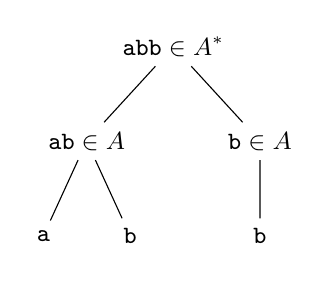
\begin{tikzpicture}[every node/.style={font=\small},
   level 1/.style={sibling distance=22mm,level distance=12mm},
   level 2/.style={sibling distance=11mm,level distance=12mm}]
  \node {$\str{abb}\in A\kstar$}
    child {node {$\str{ab}\in A$}
      child {node {$\str a$}}
      child {node {$\str b$}}}
    child {node {$\str b\in A$}
      child {node {$\str b$}}};
\end{tikzpicture}
\end{center}
So $\str{abb}=\str{ab}\concat\str b$, a $2$-piece tiling, hence $\str{abb}\in A\kstar$. But
$\str{aab}$ would have to start with a piece that is a prefix of $\str{aab}$; neither $\str{ab}$ nor
$\str b$ is, since $\str{aab}$ begins $\str{aa}$. No tiling starts, so $\str{aab}\notin A\kstar$.
\whichrule{Membership in $A\kstar$ is a left-to-right \emph{exhaustive tiling}: peel off a
prefix that lies in $A$, recurse on the rest, and accept iff some sequence of peels consumes the whole
string and leaves $\eps$.}
\emph{Check.} $\str{abb}$ tiles as $(\str{ab})(\str b)$ -- accepted. $\str{aab}$ has no first tile, so
no tiling exists -- rejected. And $\eps\in A\kstar$ via the $k=0$ empty tiling, even though
$\eps\notin A$.
\end{wex}

\begin{wex}{Star versus plus, and the empty-string subtlety}
With $A=\set{\str a}$ and $C=\set{\eps,\str a}$, compute $A\kstar,A\kplus,C\kstar,C\kplus$ and compare.
\wrec This isolates the \emph{only} difference between star and plus: whether the $k=0$ (empty)
concatenation is allowed (Def.~\ref{def:langops@c1}). The trigger ``does $\eps$ already belong to the base
language?'' decides whether star and plus coincide.
\wsol For $A=\set{\str a}$: the $k$-piece concatenations are $\str a^{k}$, so
$A\kstar=\set{\eps,\str a,\str{aa},\dots}=\set{\str a^{k}\st k\ge 0}$ and
$A\kplus=\set{\str a^{k}\st k\ge 1}$; these differ only in $\eps$. For $C=\set{\eps,\str a}$: since
$\eps\in C$, gluing in extra copies of $\eps$ changes nothing, so already $C\kplus$ contains $\eps$
(take $k=1$, piece $\eps$), giving $C\kstar=C\kplus=\set{\str a^{k}\st k\ge 0}=A\kstar$.
\begin{center}
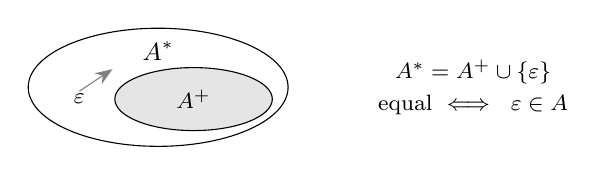
\begin{tikzpicture}[every node/.style={font=\small}]
  \node[draw,ellipse,minimum width=33mm,minimum height=15mm] (star) at (0,0) {};
  \node at (0,0.46) {$A\kstar$};
  \node[draw,ellipse,minimum width=20mm,minimum height=8mm,fill=black!10] (plus) at (0.45,-0.15) {};
  \node[font=\footnotesize] at (0.45,-0.15) {$A\kplus$};
  \node[font=\footnotesize] at (-1.0,-0.15) {$\eps$};
  \node[font=\footnotesize] at (-1.0,0.45) {};
  \draw[->,gray,shorten >=1pt] (-1.0,-0.05) -- (-0.55,0.25);
  \node[align=center,font=\footnotesize] at (4.0,0)
    {$A\kstar=A\kplus\cup\set{\eps}$\\[2pt] equal $\iff\ \eps\in A$};
\end{tikzpicture}
\end{center}
\whichrule{$A\kstar$ and $A\kplus$ differ at most by $\eps$; they are equal precisely when $\eps\in A$,
because then the $k=1$ concatenation already supplies the empty string and the $k=0$ case adds
nothing new.}
\emph{Check.} $\eps\in A\kstar\setminus A\kplus$ for $A=\set{\str a}$ (star and plus differ), while for
$C=\set{\eps,\str a}$ we have $\eps\in C$, so $C\kstar=C\kplus$.
\end{wex}

\begin{wex}{Identities for the special languages $\es$ and $\set{\eps}$}
Prove $A\concat\es=\es$, $A\concat\set{\eps}=A$, and $\es\kstar=\set{\eps}$ for every language $A$.
\wrec These are the \emph{annihilator and identity laws} for language concatenation, the analogue of
$x\cdot 0=0$ and $x\cdot 1=x$. The trigger is the appearance of the two special languages $\es$ and
$\set{\eps}$ as a concatenation factor.
\wsol By Definition~\ref{def:langops@c1}, $A\concat B=\set{xy\st x\in A,\ y\in B}$.
\begin{itemize}[leftmargin=2.2em,topsep=2pt,itemsep=1pt]
  \item $A\concat\es$: there is \emph{no} $y\in\es$ to choose, so no pair $xy$ can be formed; the set
  is empty, $A\concat\es=\es$. (Even if $A=\es$ as well, it is still $\es$.)
  \item $A\concat\set{\eps}$: the only choice for $y$ is $\eps$, and $x\eps=x$ by
  Proposition~\ref{prop:monoid@c1}, so the products are exactly the strings of $A$: $A\concat\set{\eps}=A$.
  \item $\es\kstar$: by definition star always includes the empty ($k=0$) concatenation $\eps$, and
  for $k\ge 1$ each piece would have to come from $\es$, which is impossible; so the only member is
  $\eps$, giving $\es\kstar=\set{\eps}$.
\end{itemize}
\whichrule{$\es$ is the annihilator of concatenation (like $0$ for $\times$) because it offers no right
factor, while $\set{\eps}$ is the identity (like $1$) because its only factor leaves $x$ unchanged;
star never returns $\es$ since the empty concatenation is always present.}
\emph{Check.} Contrast with union, where $\es$ is the \emph{identity}: $A\cup\es=A$. So $\es$ behaves
like $0$ for concatenation but like the additive identity for union -- different roles, same symbol.
\end{wex}

\begin{wex}{Reversal distributes over union but flips a concatenation}
For all languages $A,B$, show $\rev{(A\cup B)}=\rev A\cup\rev B$ and $\rev{(A\concat B)}=\rev B\concat
\rev A$.
\wrec Reversal of a language is reversal applied to each member (Def.~\ref{def:langops@c1}); the question
is how it interacts with $\cup$ and $\concat$. The trigger is a structural identity ``$\rev{}$ of an
operation,'' so we push $\rev{}$ inward using the string-level law (Prop.~\ref{prop:revconcat@c1}).
\wsol For union, $w\in\rev{(A\cup B)}$ iff $\rev w\in A\cup B$ iff $\rev w\in A$ or $\rev w\in B$ iff
$w\in\rev A$ or $w\in\rev B$ iff $w\in\rev A\cup\rev B$; the two sets have the same members. For
concatenation, a typical member of $A\concat B$ is $xy$ with $x\in A,y\in B$, and by
Proposition~\ref{prop:revconcat@c1} its reversal is $\rev{(xy)}=\rev y\,\rev x$ with $\rev y\in\rev B$ and
$\rev x\in\rev A$; this is exactly a member of $\rev B\concat\rev A$, and every member of $\rev
B\concat\rev A$ arises this way. Hence the order of the factors flips.
\begin{center}
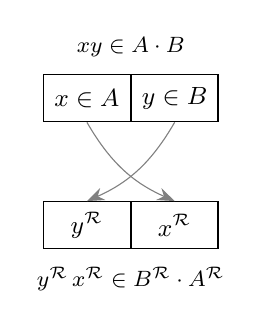
\begin{tikzpicture}[every node/.style={font=\small},node distance=6mm]
  \node[draw,minimum width=11mm,minimum height=6mm] (x) {$x\in A$};
  \node[draw,minimum width=11mm,minimum height=6mm,right=0mm of x] (y) {$y\in B$};
  \node[font=\footnotesize,above=1mm of x.north east] {$xy\in A\concat B$};
  \node[draw,minimum width=11mm,minimum height=6mm,below=10mm of x] (ry) {$\rev y$};
  \node[draw,minimum width=11mm,minimum height=6mm,right=0mm of ry] (rx) {$\rev x$};
  \node[font=\footnotesize,below=1mm of ry.south east] {$\rev y\,\rev x\in\rev B\concat\rev A$};
  \draw[->,gray] (x.south) to[bend right=18] (rx.north);
  \draw[->,gray] (y.south) to[bend left=18] (ry.north);
\end{tikzpicture}
\end{center}
\whichrule{Reversal is a \emph{set-of-images} operation, so it passes through union unchanged; against
concatenation it inherits the string-level flip $\rev{(xy)}=\rev y\,\rev x$, swapping the two
language factors.}
\emph{Check.} Take $A=\set{\str{ab}}$, $B=\set{\str{cd}}$ over $\set{\str a,\str b,\str c,\str d}$. Then
$A\concat B=\set{\str{abcd}}$, whose reversal is $\set{\str{dcba}}$, and $\rev B\concat\rev
A=\set{\str{dc}}\concat\set{\str{ba}}=\set{\str{dcba}}$ -- they match.
\end{wex}

\begin{method}{How to compute and reason about a language operation}
\begin{enumerate}[leftmargin=2em,topsep=2pt,itemsep=1pt]
  \item \textbf{Name the operation's defining set.} Write the right-hand set-builder from
  Definition~\ref{def:langops@c1}: union/intersection compare membership; concatenation forms every glued
  pair $xy$; star forms every finite list of pieces.
  \item \textbf{For concatenation, pair exhaustively, then deduplicate.} Glue each $x\in A$ to each
  $y\in B$. Expect at most $\card A\cdot\card B$ strings; fewer if two gluings collide (common over a
  one-letter alphabet).
  \item \textbf{For star, work in layers.} Compute $A^{0}=\set{\eps}$, $A^{1}=A$, $A^{2}=A\concat A$,
  $\dots$; the answer is their union. To \emph{test} membership of a single string, tile it left to
  right with pieces from $A$.
  \item \textbf{Track $\eps$ deliberately.} Decide at each step whether $\eps$ is in the result: star
  always contains it; plus contains it iff $\eps\in A$; concatenation contains it iff both factors
  contain $\eps$.
  \item \textbf{For an identity, prove two inclusions.} To show two languages are equal, show each is a
  subset of the other (``$w\in\text{LHS}\iff w\in\text{RHS}$''), pushing reversal or concatenation
  through with Propositions~\ref{prop:monoid@c1} and~\ref{prop:revconcat@c1}.
\end{enumerate}
\end{method}

\begin{pitfall}
Do not assume language concatenation is commutative or that the product count is exact.
$A\concat B$ and $B\concat A$ usually differ (string concatenation is non-commutative), and
$\card{A\concat B}$ can be \emph{strictly less} than $\card A\cdot\card B$ when distinct gluings collide
to the same string. Always glue in a fixed order and then remove duplicates.
\end{pitfall}

\begin{pitfall}
The star of a language \emph{always} contains $\eps$, regardless of whether $\eps\in A$, because the
empty ($k=0$) concatenation is by definition a member of $A\kstar$. A frequent error is to write
$A\kstar$ for a language that should exclude $\eps$; use $A\kplus$ instead, and recall
$A\kplus=A\kstar$ only when $\eps$ is already in $A$.
\end{pitfall}

\begin{exers}{Exercises.}
\item Over $\Sig=\set{\str a,\str b}$ let $w=\str{abba}$. Compute $\abs{w}$, $\rev{w}$, $w^{2}$, and
list every prefix and every suffix of $w$. Which of $\str{bb}$, $\str{ba}$, $\str{aba}$ are
substrings of $w$?

\item Let $\Sig=\set{\str0,\str1}$. Write out $\Sig^{0}$, $\Sig^{1}$, and $\Sig^{2}$ explicitly, and
say how many strings are in $\Sig^{n}$ in general. Then list the first six strings of $\Sigstar$ in
shortlex order (by length, ties broken alphabetically).

\item For strings over $\set{\str a,\str b}$, decide whether each statement is true for \emph{all}
$x,y$, giving a one-line reason or a counterexample: (a) $\abs{\rev{x}}=\abs{x}$; (b) $xy=yx$;
(c) $\rev{(\rev{x})}=x$; (d) if $x$ is a prefix of $y$ then $\rev{x}$ is a suffix of $\rev{y}$.

\item Let $A=\set{\str a,\str{ba}}$ and $B=\set{\eps,\str b}$ over $\set{\str a,\str b}$. Compute
$A\concat B$ and $B\concat A$ as explicit sets, and confirm whether $\card{A\concat B}=\card A\cdot
\card B$ in each case. Draw the gluing diagram (each $x\in A$ joined to each $y\in B$) for $A\concat
B$.

\item Let $A=\set{\str a,\str{aa}}$ over $\set{\str a}$. Compute $A^{2}=A\concat A$ and $A^{3}$ as
sets, and explain in terms of \emph{collisions} why $\card{A^{3}}<\card A^{3}$. (Hint: describe
$A^{k}$ by the lengths of strings it contains.)

\item Let $A=\set{\str{aa},\str b}$ over $\set{\str a,\str b}$. Decide, with a left-to-right tiling
argument, which of $\str{aab}$, $\str{aba}$, $\str{baab}$, $\str{aaab}$ lie in $A\kstar$. For each
member, draw the derivation tree showing how it tiles into pieces of $A$.

\item Prove that for every language $A$ one has $\es\concat A=\es$ and $\set{\eps}\concat A=A$. State
the analogous facts with the special language on the \emph{right}, and say which (if any) change when
the factors are swapped.

\item Prove or disprove, for all languages $A,B,C$ over $\Sig$: (a) $(A\cup B)\concat C=
(A\concat C)\cup(B\concat C)$; (b) $(A\cap B)\concat C=(A\concat C)\cap(B\concat C)$. For the false
one, give the smallest counterexample you can over $\set{\str a}$.

\item Show that $\rev{(\rev{A})}=A$ and $\rev{(A\kstar)}=(\rev{A})\kstar$ for every language $A$.
(For the second, use that reversal flips a concatenation (Proposition~\ref{prop:revconcat@c1}) on each
$k$-piece product.)

\item Determine, with proof, exactly when $A\kstar=A\kplus$ for a language $A$, and exactly when
$\eps\in A\concat B$. Give a single language $A$ for which $A\kstar=A\kplus$ and a single one for
which they differ.

\item \emph{Find the bug.} A classmate claims ``$A\kstar\concat A\kstar=A\kstar$ holds for every
language $A$, and also $A\kplus\concat A\kplus=A\kplus$.'' One of these is always true and one can
fail. Identify which is which, prove the true one, and give a concrete $A$ over $\set{\str a}$ where
the false one breaks.

\item \emph{Find the bug.} Someone writes: ``Since $\eps\in A\kstar$ always, and concatenating with
$\eps$ changes nothing, we have $A\concat A\kstar=A\kstar$ for every $A$.'' Show the conclusion is
false in general by testing $A=\set{\str a}$, and pinpoint the exact flaw in the reasoning. What is
the correct relationship between $A\concat A\kstar$ and $A\kplus$?
\end{exers}


\section{Logic, Quantifiers, and Boolean Connectives}
Almost every statement we will prove about machines and languages is built from a handful of
logical pieces: simple propositions glued together by \emph{connectives} (and, or, not,
implies) and ranged over by \emph{quantifiers} (for all, there exists). The one key idea of
this section is that the meaning of such a compound statement is completely determined by the
truth values of its parts, so we can always compute it mechanically -- by a truth table for the
connectives, and by a fixed rule for pushing a negation through a quantifier. Mastering these
moves now is what lets later sections say ``$\dfa$ accepts $w$ iff $\xtrans(\qstart,w)\in\Acc$''
and then negate, specialize, or chain such statements without slipping.

\subsection*{Propositions and connectives}

\begin{definition}[Proposition and truth value]
A \emph{proposition} is a statement that is either \emph{true} or \emph{false} -- never both,
never neither. Its \emph{truth value} is $\mathrm{T}$ (true) or $\mathrm{F}$ (false), often
written $1$ and $0$. ``$3$ is prime'' is a proposition (value $\mathrm{T}$); ``$x>5$'' is
\emph{not} a proposition on its own, because its value depends on $x$ -- it is a \emph{predicate}
(Definition~\ref{def:pred@c1}).
\end{definition}

\begin{definition}[Boolean connectives]\label{def:conn@c1}
Let $P,Q$ be propositions. The five basic \emph{connectives} build new propositions whose value
depends only on the values of $P$ and $Q$:
\begin{itemize}[leftmargin=2.2em,topsep=2pt,itemsep=1pt]
  \item \emph{negation} $\lnot P$ (``not $P$'') is true exactly when $P$ is false;
  \item \emph{conjunction} $P\land Q$ (``$P$ and $Q$'') is true exactly when both are true;
  \item \emph{disjunction} $P\lor Q$ (``$P$ or $Q$,'' inclusive) is true when at least one is true;
  \item \emph{implication} $P\to Q$ (``if $P$ then $Q$'') is false \emph{only} when $P$ is true and
        $Q$ is false; otherwise true;
  \item \emph{biconditional} $P\leftrightarrow Q$ (``$P$ iff $Q$'') is true exactly when $P$ and
        $Q$ have the same value.
\end{itemize}
Their meanings are fixed once and for all by the \emph{truth table}
\[
\renewcommand{\arraystretch}{1.2}
\begin{array}{cc|c|cccc}
 P & Q & \lnot P & P\land Q & P\lor Q & P\to Q & P\leftrightarrow Q\\\hline
 \mathrm{T} & \mathrm{T} & \mathrm{F} & \mathrm{T} & \mathrm{T} & \mathrm{T} & \mathrm{T}\\
 \mathrm{T} & \mathrm{F} & \mathrm{F} & \mathrm{F} & \mathrm{T} & \mathrm{F} & \mathrm{F}\\
 \mathrm{F} & \mathrm{T} & \mathrm{T} & \mathrm{F} & \mathrm{T} & \mathrm{T} & \mathrm{F}\\
 \mathrm{F} & \mathrm{F} & \mathrm{T} & \mathrm{F} & \mathrm{F} & \mathrm{T} & \mathrm{T}
\end{array}
\]
\end{definition}

The implication row deserves a long stare: $P\to Q$ is true whenever $P$ is false, no matter what
$Q$ is. A \emph{vacuously true} implication like ``if $n$ is both even and odd, then $n=0$'' costs
us nothing, and we will lean on this constantly (an empty machine accepts a string only ``if'' an
impossible condition holds). We read the two halves of a biconditional as $P\to Q$ (``only if'')
and $Q\to P$ (``if''); proving an ``iff'' means proving both arrows.

\begin{definition}[Tautology, contradiction, logical equivalence]\label{def:equiv@c1}
A compound proposition is a \emph{tautology} if it is true under every assignment of values to its
variables, and a \emph{contradiction} if it is false under every assignment. Two compound
propositions $\varphi$ and $\psi$ are \emph{logically equivalent}, written $\varphi\equiv\psi$, if
they have the same truth value under \emph{every} assignment -- equivalently, if
$\varphi\leftrightarrow\psi$ is a tautology.
\end{definition}

\begin{proposition}[The equivalences we use most]\label{prop:laws@c1}
For all propositions $P,Q,R$:
\[
\begin{array}{ll}
\textbf{(implication)} & P\to Q \;\equiv\; \lnot P\lor Q,\\[2pt]
\textbf{(contrapositive)} & P\to Q \;\equiv\; \lnot Q\to\lnot P,\\[2pt]
\textbf{(De Morgan)} & \lnot(P\land Q)\equiv \lnot P\lor\lnot Q,\qquad
                       \lnot(P\lor Q)\equiv \lnot P\land\lnot Q,\\[2pt]
\textbf{(distributive)} & P\land(Q\lor R)\equiv(P\land Q)\lor(P\land R).
\end{array}
\]
\end{proposition}
\begin{proof}
Each is a claim that two columns of a truth table agree, so it suffices to fill in the table and
compare. We do the contrapositive; the others are identical in spirit, and one De Morgan law is
filled in as Worked Example~\ref{wex:demorgan@c1} below.
\[
\renewcommand{\arraystretch}{1.2}
\begin{array}{cc|cc|c|c}
 P & Q & \lnot Q & \lnot P & P\to Q & \lnot Q\to\lnot P\\\hline
 \mathrm{T} & \mathrm{T} & \mathrm{F} & \mathrm{F} & \mathrm{T} & \mathrm{T}\\
 \mathrm{T} & \mathrm{F} & \mathrm{T} & \mathrm{F} & \mathrm{F} & \mathrm{F}\\
 \mathrm{F} & \mathrm{T} & \mathrm{F} & \mathrm{T} & \mathrm{T} & \mathrm{T}\\
 \mathrm{F} & \mathrm{F} & \mathrm{T} & \mathrm{T} & \mathrm{T} & \mathrm{T}
\end{array}
\]
The last two columns are identical, so $P\to Q\equiv\lnot Q\to\lnot P$.
\end{proof}

The single most useful way to \emph{see} the meaning of a connective is to read it as a small
decision procedure on the two input bits. The next figure draws $P\to Q$ this way: the only path
that reaches ``false'' is $P$ true followed by $Q$ false.

\begin{center}
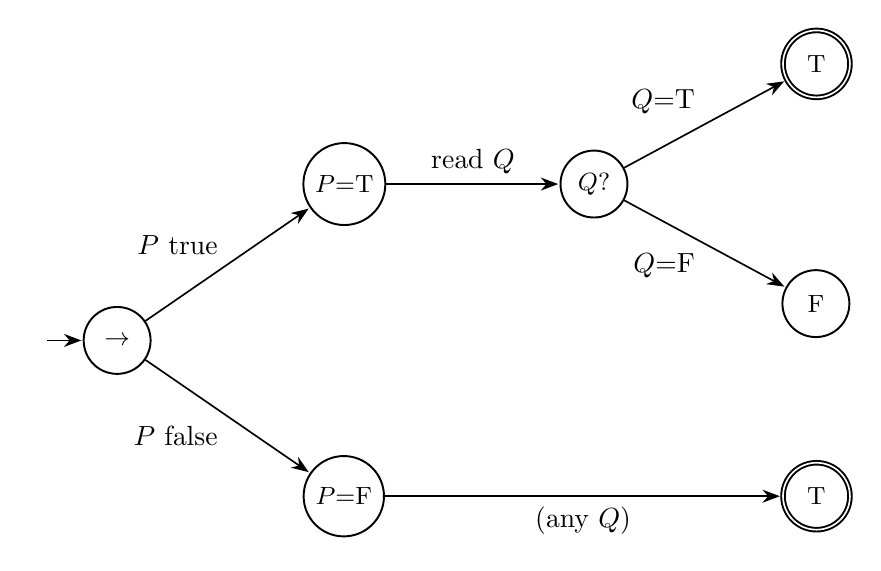
\begin{tikzpicture}[fa,node distance=13mm and 22mm]
  \node[stinit] (start) {$\to$};
  \node[st,above right=of start,inner sep=3pt] (pt) {$P{=}\mathrm{T}$};
  \node[st,below right=of start,inner sep=3pt] (pf) {$P{=}\mathrm{F}$};
  \node[st,right=of pt] (out1) {$Q$?};
  \node[stacc,above right=9mm and 22mm of out1] (T1) {$\mathrm{T}$};
  \node[st,below right=9mm and 22mm of out1] (F1) {$\mathrm{F}$};
  \node[stacc] (T2) at (pf -| T1) {$\mathrm{T}$};
  \path (start) edge node{$P$ true} (pt)
        (start) edge node[swap]{$P$ false} (pf)
        (pt) edge node{read $Q$} (out1)
        (out1) edge node{$Q{=}\mathrm{T}$} (T1)
        (out1) edge node[swap]{$Q{=}\mathrm{F}$} (F1)
        (pf) edge node[swap]{(any $Q$)} (T2);
\end{tikzpicture}
\end{center}

\begin{wex}{Build a truth table for a three-variable formula}\label{wex:table3@c1}
Decide whether $\varphi=(P\to Q)\land(Q\to R)\to(P\to R)$ is a tautology.
\wrec The formula mixes connectives over three variables and asks ``true under \emph{every}
assignment?'' The trigger ``every assignment / is it a tautology'' says: enumerate all
$2^3=8$ rows of a truth table and check the final column. (This is the transitivity of
implication, the backbone of chaining lemmas.)
\wsol List the eight assignments and evaluate inside-out. Write $A=P\to Q$, $B=Q\to R$,
$C=P\to R$; the formula is $(A\land B)\to C$.
\[
\renewcommand{\arraystretch}{1.15}
\begin{array}{ccc|ccc|c|c}
 P & Q & R & A & B & C & A\land B & (A\land B)\to C\\\hline
 \mathrm{T}&\mathrm{T}&\mathrm{T} & \mathrm{T}&\mathrm{T}&\mathrm{T} & \mathrm{T} & \mathrm{T}\\
 \mathrm{T}&\mathrm{T}&\mathrm{F} & \mathrm{T}&\mathrm{F}&\mathrm{F} & \mathrm{F} & \mathrm{T}\\
 \mathrm{T}&\mathrm{F}&\mathrm{T} & \mathrm{F}&\mathrm{T}&\mathrm{T} & \mathrm{F} & \mathrm{T}\\
 \mathrm{T}&\mathrm{F}&\mathrm{F} & \mathrm{F}&\mathrm{T}&\mathrm{F} & \mathrm{F} & \mathrm{T}\\
 \mathrm{F}&\mathrm{T}&\mathrm{T} & \mathrm{T}&\mathrm{T}&\mathrm{T} & \mathrm{T} & \mathrm{T}\\
 \mathrm{F}&\mathrm{T}&\mathrm{F} & \mathrm{T}&\mathrm{F}&\mathrm{T} & \mathrm{F} & \mathrm{T}\\
 \mathrm{F}&\mathrm{F}&\mathrm{T} & \mathrm{T}&\mathrm{T}&\mathrm{T} & \mathrm{T} & \mathrm{T}\\
 \mathrm{F}&\mathrm{F}&\mathrm{F} & \mathrm{T}&\mathrm{T}&\mathrm{T} & \mathrm{T} & \mathrm{T}
\end{array}
\]
Every entry in the last column is $\mathrm{T}$, so $\varphi$ is a tautology.
\whichrule{A claim of the form ``$\varphi$ holds for every assignment'' is exactly a tautology
check, and with $k$ variables the complete, decisive method is the $2^k$-row truth table -- here
$2^3=8$ rows settle it with no cleverness required.}
\emph{Check.} The only way $(A\land B)\to C$ could be false is $A\land B$ true and $C$ false; that
needs $P\to Q$, $Q\to R$ both true yet $P\to R$ false, i.e.\ $P=\mathrm{T},R=\mathrm{F}$. Then
$P\to Q$ forces $Q=\mathrm{T}$, but $Q\to R$ then forces $R=\mathrm{T}$, a contradiction. No bad
row exists, matching the table.
\end{wex}

\begin{wex}{Verify a De Morgan law by table}\label{wex:demorgan@c1}
Show $\lnot(P\lor Q)\equiv \lnot P\land\lnot Q$.
\wrec We must show two formulas agree on \emph{every} assignment -- that is a logical-equivalence
claim (Definition~\ref{def:equiv@c1}). The trigger ``$\varphi\equiv\psi$'' says: tabulate both and
check the columns are identical.
\wsol Four rows suffice (two variables):
\[
\renewcommand{\arraystretch}{1.2}
\begin{array}{cc|c|c|cc|c}
 P & Q & P\lor Q & \lnot(P\lor Q) & \lnot P & \lnot Q & \lnot P\land\lnot Q\\\hline
 \mathrm{T}&\mathrm{T} & \mathrm{T} & \mathrm{F} & \mathrm{F} & \mathrm{F} & \mathrm{F}\\
 \mathrm{T}&\mathrm{F} & \mathrm{T} & \mathrm{F} & \mathrm{F} & \mathrm{T} & \mathrm{F}\\
 \mathrm{F}&\mathrm{T} & \mathrm{T} & \mathrm{F} & \mathrm{T} & \mathrm{F} & \mathrm{F}\\
 \mathrm{F}&\mathrm{F} & \mathrm{F} & \mathrm{T} & \mathrm{T} & \mathrm{T} & \mathrm{T}
\end{array}
\]
The columns $\lnot(P\lor Q)$ and $\lnot P\land\lnot Q$ are identical, so the two are equivalent.
\whichrule{Negating a disjunction turns ``or'' into ``and'' and flips each operand; the table is
the airtight justification, and the pattern is what we will use to negate quantifiers below.}
\emph{Check.} ``It is not the case that ($P$ or $Q$)'' should mean ``neither $P$ nor $Q$,'' which
is exactly $\lnot P$ and $\lnot Q$ -- the English matches the table.
\end{wex}

\subsection*{Predicates and quantifiers}

\begin{definition}[Predicate]\label{def:pred@c1}
A \emph{predicate} on a set $D$ is a function $P\colon D\to\set{\mathrm{T},\mathrm{F}}$; we write
$P(x)$ for its value at $x\in D$ and call $D$ the \emph{domain of discourse}. A $k$-ary predicate
takes $k$ arguments, $P(x_1,\dots,x_k)$. Predicates over strings are everywhere in this book:
e.g.\ $\mathrm{Acc}_{\dfa}(w)$ = ``$\dfa$ accepts $w$,'' a predicate on $w\in\Sigstar$.
\end{definition}

\begin{definition}[Quantifiers]\label{def:quant@c1}
Let $P$ be a predicate on a domain $D$.
\begin{itemize}[leftmargin=2.2em,topsep=2pt,itemsep=1pt]
  \item The \emph{universal} statement $\forall x\,P(x)$ (``for all $x$, $P(x)$'') is true iff
        $P(x)$ is true for \emph{every} $x\in D$.
  \item The \emph{existential} statement $\exists x\,P(x)$ (``there exists $x$ with $P(x)$'') is
        true iff $P(x)$ is true for \emph{at least one} $x\in D$.
\end{itemize}
On a finite domain $D=\set{x_1,\dots,x_n}$ these unfold into connectives:
$\forall x\,P(x)\equiv P(x_1)\land\cdots\land P(x_n)$ and
$\exists x\,P(x)\equiv P(x_1)\lor\cdots\lor P(x_n)$.
\end{definition}

The finite-domain unfolding is the bridge between this subsection and the last: $\forall$ is a big
``and,'' $\exists$ is a big ``or.'' Everything about negating quantifiers follows by pushing De
Morgan through that unfolding.

\begin{theorem}[Negation of quantifiers]\label{thm:negquant@c1}
For any predicate $P$ on any domain,
\[
  \lnot\,\forall x\,P(x)\ \equiv\ \exists x\,\lnot P(x),
  \qquad
  \lnot\,\exists x\,P(x)\ \equiv\ \forall x\,\lnot P(x).
\]
\end{theorem}
\begin{proof}
Read the left equivalence directly: ``not every $x$ satisfies $P$'' means \emph{some} $x$ fails
$P$, i.e.\ some $x$ satisfies $\lnot P$. The right is dual. To see it is forced rather than merely
plausible, take a finite domain $\set{x_1,\dots,x_n}$ and unfold (Definition~\ref{def:quant@c1}):
\[
  \lnot\,\forall x\,P(x)\ \equiv\ \lnot\bigl(P(x_1)\land\cdots\land P(x_n)\bigr)
  \ \equiv\ \lnot P(x_1)\lor\cdots\lor\lnot P(x_n)\ \equiv\ \exists x\,\lnot P(x),
\]
where the middle step is De Morgan (Proposition~\ref{prop:laws@c1}) applied $n-1$ times. The
existential case unfolds to a disjunction and negates to a conjunction the same way; the argument
extends to infinite domains because the meaning of $\forall$/$\exists$ is exactly ``all''/``some.''
\end{proof}

\begin{corollary}[Pushing negation through a chain]\label{cor:push@c1}
To negate a string of quantifiers, swap each $\forall$ with $\exists$ and each $\exists$ with
$\forall$, walking left to right, and negate the innermost predicate. For example,
\[
  \lnot\,\forall x\,\exists y\,\forall z\;R(x,y,z)
  \ \equiv\ \exists x\,\forall y\,\exists z\;\lnot R(x,y,z).
\]
\end{corollary}
\begin{proof}
Apply Theorem~\ref{thm:negquant@c1} once per quantifier, outermost first: each application moves the
$\lnot$ one quantifier inward and flips that quantifier's type, until the $\lnot$ lands on $R$.
\end{proof}

A quantified statement is best read as a \emph{nesting}: each quantifier owns everything to its
right (its \emph{scope}). The tree below shows the scope structure of $\forall x\,\exists y\,
R(x,y)$ and where a negation lands after Corollary~\ref{cor:push@c1} turns it into $\exists x\,
\forall y\,\lnot R(x,y)$.

\begin{center}
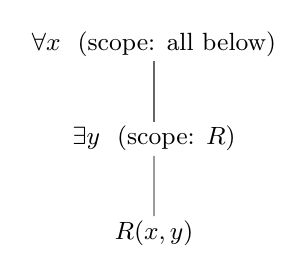
\begin{tikzpicture}[treenode,level distance=12mm,
   level 1/.style={sibling distance=42mm},
   level 2/.style={sibling distance=42mm},
   edge from parent/.style={tedge,draw}]
  \node {$\forall x$ \ (scope: all below)}
    child {node {$\exists y$ \ (scope: $R$)}
      child {node {$R(x,y)$}}};
\end{tikzpicture}
\qquad
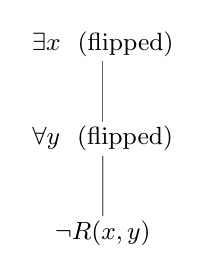
\begin{tikzpicture}[treenode,level distance=12mm,
   level 1/.style={sibling distance=42mm},
   level 2/.style={sibling distance=42mm},
   edge from parent/.style={tedge,draw}]
  \node {$\exists x$ \ (flipped)}
    child {node {$\forall y$ \ (flipped)}
      child {node {$\lnot R(x,y)$}}};
\end{tikzpicture}
\end{center}

\begin{wex}{Negate a real definition: ``$\dfa$ accepts every string''}\label{wex:negaccept@c1}
The statement ``$\dfa$ accepts every string over $\Sig$'' is
$\forall w\in\Sigstar\;\mathrm{Acc}_{\dfa}(w)$. Write its negation in plain words and in symbols.
\wrec This asks to negate a \emph{universal} statement over strings -- exactly
Theorem~\ref{thm:negquant@c1}. The trigger ``write the negation of `for all \dots' '' says: turn
$\forall$ into $\exists$ and negate the body.
\wsol By Theorem~\ref{thm:negquant@c1},
\[
  \lnot\,\forall w\;\mathrm{Acc}_{\dfa}(w)\ \equiv\ \exists w\;\lnot\mathrm{Acc}_{\dfa}(w),
\]
and $\lnot\mathrm{Acc}_{\dfa}(w)$ is ``$\dfa$ rejects $w$.'' In words: \emph{$\dfa$ fails to accept
every string iff there is some string $\dfa$ rejects.} So to refute ``accepts everything'' you need
exactly \emph{one} rejected string -- a single counterexample.
\whichrule{The negation of a universal is an existential with the body negated; the practical
payoff is that disproving a ``for all'' claim is a search for one witness, never a re-proof over
all inputs.}
\emph{Check.} If $\lang{\dfa}=\Sigstar$ then no witness $w$ exists, the existential is false, and
the original $\forall$ is true -- the equivalence behaves correctly at the extreme.
\end{wex}

\begin{wex}{Order of quantifiers changes the meaning}\label{wex:order@c1}
On the domain $\Z$, compare $\forall x\,\exists y\,(x+y=0)$ with $\exists y\,\forall x\,(x+y=0)$.
\wrec Two statements use the same predicate but swap the quantifier order. The trigger
``$\forall\exists$ vs.\ $\exists\forall$'' says: read each as a nested game and ask who moves
first, because the inner choice may legally depend on the outer one.
\wsol In $\forall x\,\exists y\,(x+y=0)$ the value of $y$ is chosen \emph{after} $x$ is fixed, so
we may take $y=-x$; the statement is \textbf{true}. In $\exists y\,\forall x\,(x+y=0)$ a single $y$
must work for \emph{all} $x$ at once; no fixed $y$ satisfies $x+y=0$ for two different $x$, so the
statement is \textbf{false}. Same atoms, opposite truth values.
\begin{center}
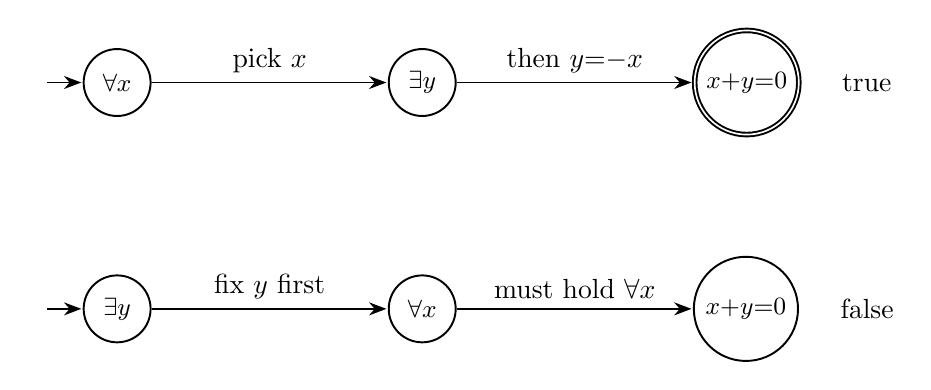
\begin{tikzpicture}[fa,node distance=12mm and 30mm]
  \node[stinit] (a0) {$\forall x$};
  \node[st,right=of a0] (a1) {$\exists y$};
  \node[stacc,right=of a1,inner sep=3pt] (a2) {$x{+}y{=}0$};
  \node[stinit,below=20mm of a0] (b0) {$\exists y$};
  \node[st,right=of b0] (b1) {$\forall x$};
  \node[st,right=of b1,inner sep=3pt] (b2) {$x{+}y{=}0$};
  \path (a0) edge node{pick $x$} (a1)
        (a1) edge node{then $y{=}{-}x$} (a2)
        (b0) edge node{fix $y$ first} (b1)
        (b1) edge node{must hold $\forall x$} (b2);
  \node[right=4mm of a2] {true};
  \node[right=4mm of b2] {false};
\end{tikzpicture}
\end{center}
\whichrule{In $\forall x\,\exists y$ the witness $y$ may depend on $x$; in $\exists y\,\forall x$
one witness must serve every $x$. Swapping the two quantifiers is therefore \emph{not} a
truth-preserving move, unlike swapping two adjacent $\forall$s or two adjacent $\exists$s.}
\emph{Check.} The order $\exists\forall$ is logically stronger: $\exists y\,\forall x\,P\to
\forall x\,\exists y\,P$ always holds (the universal witness also works pointwise), but the
converse fails here -- consistent with $\mathrm{F}\to\mathrm{T}$ being true and $\mathrm{T}\to\mathrm{F}$ false.
\end{wex}

\subsection*{Predicates as relations, and a circuit view}

A binary predicate $R(x,y)$ on a finite set is the same data as a directed graph: draw an arrow
from $x$ to $y$ exactly when $R(x,y)$ is true. This is the picture that makes properties like
reflexivity and symmetry visible at a glance, and it is the same drawing convention we use for
state diagrams.

\begin{wex}{Read a relation off its graph, then negate a property}\label{wex:relgraph@c1}
On $D=\set{1,2,3}$ let $R$ be ``$x$ divides $y$'' ($x\mid y$). Draw $R$ as a directed graph and
decide whether $\forall x\,\exists y\,(x\neq y\land R(x,y))$ holds.
\wrec A binary predicate on a small finite set is a directed graph (an arrow for each true pair),
and the question is a $\forall\exists$ statement over that graph. The trigger ``binary predicate +
small finite domain'' says: draw the arrows, then check the quantified claim node by node.
\wsol The true pairs of $x\mid y$ on $\set{1,2,3}$ are $(1,1),(2,2),(3,3),(1,2),(1,3)$. Drawing
them (self-loops are the reflexive pairs $x\mid x$):
\begin{center}
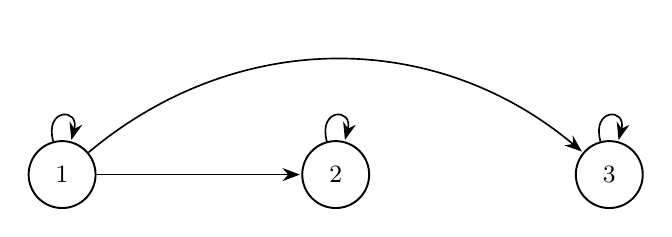
\begin{tikzpicture}[fa,node distance=22mm and 26mm]
  \node[st] (n1) {$1$};
  \node[st,right=of n1] (n2) {$2$};
  \node[st,right=of n2] (n3) {$3$};
  \path (n1) edge[loop above] node{} (n1)
        (n2) edge[loop above] node{} (n2)
        (n3) edge[loop above] node{} (n3)
        (n1) edge node{} (n2)
        (n1) edge[bend left=40] node{} (n3);
\end{tikzpicture}
\end{center}
Now test $\forall x\,\exists y\,(x\neq y\land x\mid y)$: $x{=}1$ has the witness $y{=}2$
($1\neq2$, $1\mid2$). But $x{=}2$ has \emph{no} $y\neq2$ in $\set{1,2,3}$ with $2\mid y$ (only
$2\mid2$, excluded by $x\neq y$). So the $\forall$ fails at $x{=}2$; the statement is \textbf{false}.
By Theorem~\ref{thm:negquant@c1} its negation $\exists x\,\forall y\,(x=y\lor\lnot R(x,y))$ holds, and
$x{=}2$ is the witness.
\whichrule{A binary relation on a finite domain is exactly a directed graph, so reflexivity =
``a loop at every node'' and a $\forall\exists$ claim = ``every node has an outgoing arrow to a
\emph{different} node''; node $2$ has only its self-loop, which both kills the claim and is the
explicit witness for the negation.}
\emph{Check.} Count outgoing non-loop arrows: node $1$ has two, nodes $2$ and $3$ have none.
``Every node has a non-loop out-arrow'' is therefore false, witnessed by $2$ (or $3$).
\end{wex}

\begin{wex}{A connective as a logic gate}\label{wex:gate@c1}
Express the exclusive-or $P\oplus Q$ (true iff exactly one of $P,Q$ is true) with $\land,\lor,\lnot$,
and draw it as a gate network.
\wrec ``Exactly one is true'' is a custom connective; the trigger ``define a new connective from
the basic ones'' says: write its truth table, read off the true rows, and assemble an
$\lor$-of-$\land$s (a disjunctive normal form).
\wsol $P\oplus Q$ is true on the rows $(P,Q)=(\mathrm{T},\mathrm{F})$ and
$(\mathrm{F},\mathrm{T})$, giving
$P\oplus Q\equiv(P\land\lnot Q)\lor(\lnot P\land Q)$. As a network of gates, two AND gates each
take one plain and one negated input, and their outputs feed a single OR:
\begin{center}
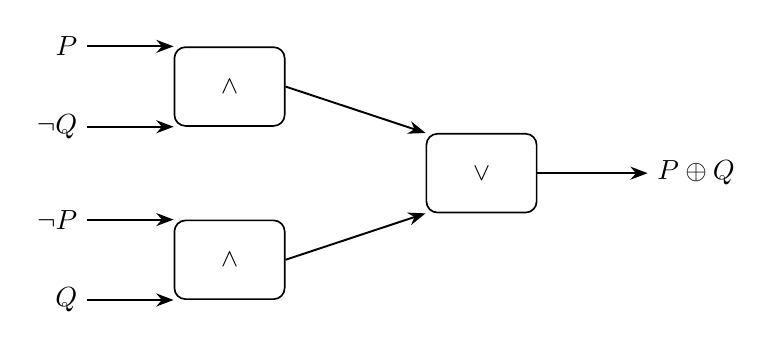
\begin{tikzpicture}[
   gate/.style={procbox,minimum width=14mm,minimum height=10mm},
   wire/.style={flow}]
  \node[gate] (a1) at (0,1.1) {$\land$};
  \node[gate] (a2) at (0,-1.1) {$\land$};
  \node[gate] (orr) at (3.2,0) {$\lor$};
  % input stubs for the top AND gate
  \node[left=11mm of a1.north west,anchor=east] (p1) {$P$};
  \node[left=11mm of a1.south west,anchor=east] (q1) {$\lnot Q$};
  % input stubs for the bottom AND gate
  \node[left=11mm of a2.north west,anchor=east] (p2) {$\lnot P$};
  \node[left=11mm of a2.south west,anchor=east] (q2) {$Q$};
  \draw[wire] (p1) -- (a1.north west);
  \draw[wire] (q1) -- (a1.south west);
  \draw[wire] (p2) -- (a2.north west);
  \draw[wire] (q2) -- (a2.south west);
  \draw[wire] (a1.east) -- (orr.north west);
  \draw[wire] (a2.east) -- (orr.south west);
  \node[right=14mm of orr] (out) {$P\oplus Q$};
  \draw[wire] (orr.east) -- (out);
\end{tikzpicture}
\end{center}
\whichrule{Any connective is determined by its true rows, and ``OR together one AND-clause per
true row'' (disjunctive normal form) realizes it from $\land,\lor,\lnot$ alone -- so $\set{\land,
\lor,\lnot}$ is a complete set of connectives, with XOR a derived gate.}
\emph{Check.} On $(P,Q)=(\mathrm{T},\mathrm{T})$ both AND-clauses are false (each needs a negated
true input), so the OR is false -- correct, since XOR is false when both agree.
\end{wex}

\begin{method}{How to negate a quantified statement cleanly}
\begin{enumerate}[leftmargin=2em,topsep=2pt,itemsep=1pt]
  \item \textbf{Put it in prefix form:} all quantifiers up front, a quantifier-free body at the end,
        e.g.\ $\forall x\,\exists y\;\Phi(x,y)$.
  \item \textbf{Walk the quantifiers left to right}, flipping each: $\forall\leftrightarrow\exists$.
        Do not reorder them -- order carries meaning (Worked Example~\ref{wex:order@c1}).
  \item \textbf{Negate the body $\Phi$} using the connective laws (Proposition~\ref{prop:laws@c1}):
        $\lnot(A\land B)=\lnot A\lor\lnot B$, $\lnot(A\lor B)=\lnot A\land\lnot B$,
        $\lnot(A\to B)=A\land\lnot B$, and $\lnot\lnot A=A$.
  \item \textbf{Translate back to English} and sanity-check against a tiny domain (one or two
        elements) where you can see both the statement and its negation by hand.
\end{enumerate}
\end{method}

\begin{pitfall}
The negation of $P\to Q$ is \emph{not} $P\to\lnot Q$, and it is not $\lnot P\to\lnot Q$. Since
$P\to Q\equiv\lnot P\lor Q$, its negation is $\lnot(\lnot P\lor Q)\equiv P\land\lnot Q$: ``$P$ is
true \emph{and} $Q$ is false.'' Concretely, the negation of ``if $w$ is accepted then $w$ ends in
$\str1$'' is ``$w$ is accepted \emph{and} $w$ does not end in $\str1$,'' a single conjunction you
can exhibit, not another implication.
\end{pitfall}

\begin{pitfall}
Do not swap adjacent quantifiers of \emph{different} type. $\forall x\,\exists y\,R(x,y)$ and
$\exists y\,\forall x\,R(x,y)$ are genuinely different statements (Worked
Example~\ref{wex:order@c1}); only the direction $\exists\forall\Rightarrow\forall\exists$ is always
valid. Reordering two $\forall$s with each other, or two $\exists$s with each other, is harmless;
mixing the types is where proofs silently go wrong.
\end{pitfall}

\begin{pitfall}
``$P$ or $Q$'' in mathematics is \emph{inclusive}: it is true when both hold. If you mean ``exactly
one,'' you want exclusive-or $P\oplus Q$ (Worked Example~\ref{wex:gate@c1}), which is a different,
non-basic connective. Reading a mathematical ``or'' as exclusive is a common source of off-by-one
errors when you later count the strings a machine accepts.
\end{pitfall}

The four negation laws of this section -- two for connectives, two for quantifiers -- are not four
separate facts to memorize but one idea seen from four sides: \emph{negation is duality}. Pushing a
$\lnot$ inward swaps each operator for its dual ($\land\leftrightarrow\lor$,
$\forall\leftrightarrow\exists$) while negating what is inside, and the result is always logically
equivalent to the original. The map below collects all four under that single principle.

% FIG 1A -- LOCAL CONCEPT MAP: De Morgan duality (negation).
%   Placement: end of Section 3 (Logic, Quantifiers, Boolean Connectives), after the
%     connective and quantifier-negation material (post-pitfalls).
%   Purpose: unify the four negation laws under one idea -- "negation is duality".
%   Objects: central croot "Negation = duality"; four cnodes, one per law (two De Morgan
%     for connectives, two quantifier-negation rules).
%   Arrows (cedge) from root to each law, labelled (cedgelbl) "connectives" / "quantifiers".
%   Invariant: each law is a logical equivalence (same truth value under every assignment /
%     same models), i.e. a tautological equivalence.
%   Caption (takeaway): negation turns each connective/quantifier into its dual while negating
%     the inside; truth values are preserved.
%   Validation: these are exactly the De Morgan laws for connectives and the standard
%     quantifier-negation rules, each a tautological equivalence.
\begin{center}
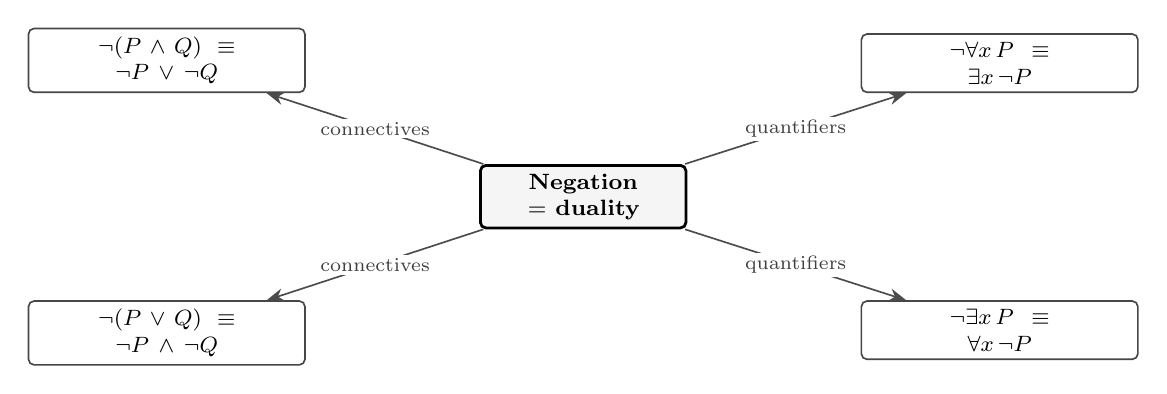
\begin{tikzpicture}[node distance=10mm and 18mm]
  \node[croot,text width=24mm] (root) {Negation\\$=$ duality};
  \node[cnode,text width=33mm,above left=9mm and 22mm of root] (and)
    {$\lnot(P\land Q)\equiv$\\$\lnot P\lor\lnot Q$};
  \node[cnode,text width=33mm,below left=9mm and 22mm of root] (or)
    {$\lnot(P\lor Q)\equiv$\\$\lnot P\land\lnot Q$};
  \node[cnode,text width=33mm,above right=9mm and 22mm of root] (all)
    {$\lnot\forall x\,P\equiv$\\$\exists x\,\lnot P$};
  \node[cnode,text width=33mm,below right=9mm and 22mm of root] (ex)
    {$\lnot\exists x\,P\equiv$\\$\forall x\,\lnot P$};
  \draw[cedge] (root) -- (and) node[cedgelbl,midway]{connectives};
  \draw[cedge] (root) -- (or)  node[cedgelbl,midway]{connectives};
  \draw[cedge] (root) -- (all) node[cedgelbl,midway]{quantifiers};
  \draw[cedge] (root) -- (ex)  node[cedgelbl,midway]{quantifiers};
\end{tikzpicture}
\end{center}

\noindent\emph{Negation turns each connective or quantifier into its dual --
$\land\leftrightarrow\lor$, $\forall\leftrightarrow\exists$ -- while negating the inside; truth
values are preserved, so each arrow is a logical equivalence, not just a rewrite.}
\emph{Check.} The two left laws are exactly the De Morgan laws (one of them verified by table in Worked
Example~\ref{wex:demorgan@c1}); the two right laws are Theorem~\ref{thm:negquant@c1}, which the finite-domain
unfolding reduces to those same De Morgan laws -- so all four are one tautological equivalence wearing
four faces.

\begin{exers}{Exercises.}
\item Build the full truth table for $(P\lor Q)\to(P\land Q)$. Is it a tautology, a contradiction,
or neither? In one sentence, describe in plain English the assignments on which it is false.

\item Use a truth table to decide whether $P\to(Q\to R)$ and $(P\land Q)\to R$ are logically
equivalent. If they are, say in words why ``$P$ implies that $Q$ implies $R$'' should mean the same
as ``$P$ and $Q$ together imply $R$.''

\item Verify the second De Morgan law $\lnot(P\land Q)\equiv\lnot P\lor\lnot Q$ by truth table, then
use it together with $P\to Q\equiv\lnot P\lor Q$ to rewrite $\lnot(P\to Q)$ as a conjunction with no
arrow and no outer negation.

\item Show by truth table that $\set{\lnot,\to\,}$ is a complete connective set by expressing both
$P\lor Q$ and $P\land Q$ using only $\lnot$ and $\to$. (Hint: start from $P\to Q\equiv\lnot P\lor Q$.)

\item Let the domain be $\Z$. Write each statement in symbols, then write its negation in symbols and
in plain English: (a) every integer has an additive inverse; (b) some integer is its own square;
(c) for every $x$ there is a $y$ with $y>x$.

\item Negate the statement $\forall x\,\exists y\,\forall z\,\bigl(R(x,y)\land(R(y,z)\to R(x,z))\bigr)$,
pushing the negation all the way to the predicates so that no $\lnot$ stands in front of a quantifier
or in front of a parenthesis.

\item On the domain $D=\set{0,1,2,3}$ let $E(x)$ mean ``$x$ is even'' and $L(x,y)$ mean ``$x<y$.''
Decide the truth value of each, justifying with a witness or a counterexample:
(a) $\forall x\,(E(x)\lor\exists y\,L(x,y))$; (b) $\exists y\,\forall x\,L(x,y)$;
(c) $\forall x\,\exists y\,(L(x,y)\land E(y))$.

\item Define a predicate over strings: for $w\in\set{0,1}\kstar$ let $P(w)$ mean ``$w$ contains at
least one $\str1$.'' Express ``$w$ is the all-zeros string (possibly empty)'' using $P$ and a
negation, and express ``$w$ has at least two $\str1$s'' using two quantifiers over positions of $w$.

\item On $D=\set{1,2,3,4}$ let $R(x,y)$ mean ``$x+y$ is even.'' Draw $R$ as a directed graph (an
arrow $x\to y$ whenever $R(x,y)$ is true; include self-loops). From your drawing, decide whether $R$
is reflexive, whether it is symmetric, and whether $\forall x\,\exists y\,(x\neq y\land R(x,y))$ holds.

\item Give a connective expression for the ``majority'' function $\mathrm{Maj}(P,Q,R)$, true iff at
least two of $P,Q,R$ are true, as an OR of AND-clauses (one clause per true row of its table). Then
draw it as a gate network with four AND gates feeding one OR gate.

\item \emph{Find the bug.} A student writes: ``The negation of `for all $x$, if $x>0$ then
$x^2>0$' is `for all $x$, if $x>0$ then $x^2\le 0$.' '' Identify every error (there are two: the
quantifier and the body), and write the correct negation in symbols and in English.

\item \emph{Find the bug.} Someone claims $\forall x\,\exists y\,(x\cdot y=1)$ is true over $\Z$
``because you can always take $y=1/x$.'' Explain precisely why the argument fails, name a
domain on which the statement \emph{is} true with the same predicate, and state the correct truth
value over $\Z$.

\item Prove that for any predicate $P$ on any domain, $\exists y\,\forall x\,P(x,y)$ logically
implies $\forall x\,\exists y\,P(x,y)$, but the converse fails. (For the failure, exhibit a small
domain and a concrete $P$.) Explain in one sentence which quantifier order is the ``stronger''
statement and why.
\end{exers}


\section{Methods of Proof}
A definition tells you what an object \emph{is}; a theorem asserts that some objects have a
property; a proof is the airtight argument that forces you to believe the theorem. This section is
about the small number of \emph{shapes} a proof can take. The one key idea is that the logical form
of the statement you want to prove -- an implication, an ``if and only if,'' an existence claim, a
universal claim -- dictates the skeleton of the argument, and once you can read that form off the
statement, you know which of a handful of standard openings to write down. Everything later in this
book (that a construction works, that two machines are equivalent, that some language is \emph{not}
regular) is one of these shapes dressed in the costume of automata, so it pays to see the shapes
bare. We treat the five workhorses -- direct proof, proof by contrapositive, proof by contradiction,
proof by construction, and proof by cases -- and pair each with a worked argument and, for all but
construction, a diagram of its logical flow.

\subsection*{Reading a statement before proving it}

Most proofs stall not on cleverness but on misreading the claim. Before writing anything, rewrite
the statement so its logical form is explicit.

\begin{definition}[The four common forms]\label{def:forms@c1}
Let $P,Q$ be predicates (statements that may be true or false, possibly depending on a variable).
The forms we meet constantly are:
\begin{itemize}[leftmargin=2.2em,topsep=2pt,itemsep=1pt]
  \item \emph{Implication} ``$P\imp Q$'': if $P$ holds then $Q$ holds. By definition this is false in
  exactly one situation -- $P$ true while $Q$ false.
  \item \emph{Biconditional} ``$P\eqv Q$'': both $P\imp Q$ and $Q\imp P$. Proving it means proving
  \emph{two} implications, the forward and the reverse.
  \item \emph{Universal} ``for all $x$, $R(x)$'': $R$ holds of every $x$ in the intended domain. A
  single $x$ with $R(x)$ false (a \emph{counterexample}) refutes it.
  \item \emph{Existential} ``there exists $x$ with $R(x)$'': at least one $x$ makes $R$ true.
  Producing one such $x$ proves it.
\end{itemize}
\end{definition}

The negations are worth memorizing, because contrapositive and contradiction both run on them: the
negation of ``$P\imp Q$'' is ``$P$ and not $Q$''; the negation of ``for all $x$, $R(x)$'' is ``there
exists $x$ with not $R(x)$''; and the negation of ``there exists $x$, $R(x)$'' is ``for all $x$, not
$R(x)$.'' A quantifier flips when you push a negation past it.

\begin{definition}[Contrapositive and converse]\label{def:contra@c1}
The \emph{contrapositive} of ``$P\imp Q$'' is ``$(\text{not }Q)\imp(\text{not }P)$''; it is logically
\emph{equivalent} to the original, so proving one proves the other. The \emph{converse} ``$Q\imp P$''
is a \emph{different} statement and may be true or false independently.
\end{definition}

Confusing the contrapositive (always equivalent, a legitimate proof target) with the converse (a
separate claim) is the single most common logical error, so keep them straight from the start.

\subsection*{The five methods}

We state each method as a recipe, then prove a small theorem in that style. The accompanying diagram
shows the \emph{logical flow}: what you are allowed to assume and what you must reach.

\textbf{1. Direct proof of an implication.} To prove $P\imp Q$: assume $P$, and by a forward chain of
definitions and prior results, deduce $Q$. The flow is a straight line.
\begin{center}
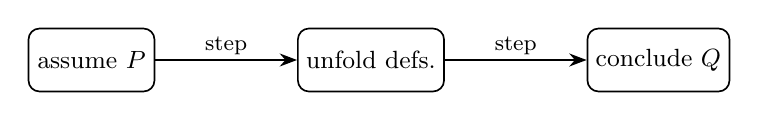
\begin{tikzpicture}[node distance=8mm]
  \node[procbox] (P) {assume $P$};
  \node[procbox,right=18mm of P] (mid) {unfold defs.};
  \node[procbox,right=18mm of mid] (Q) {conclude $Q$};
  \path (P) edge[flow] node[flowlbl,above]{step} (mid)
        (mid) edge[flow] node[flowlbl,above]{step} (Q);
\end{tikzpicture}
\end{center}

\begin{wex}{Direct proof: the product of two even integers is even}
Prove: if $m$ and $n$ are even integers, then $mn$ is even.
\wrec The statement is a bare implication ``$P\imp Q$'' with a friendly hypothesis (``even'' has a
clean algebraic meaning), and $Q$ follows by substitution. That ease is the trigger for a
\emph{direct} proof: assume $P$ and compute toward $Q$.
\wsol Assume $m$ and $n$ are even. By the definition of even, $m=2a$ and $n=2b$ for some integers
$a,b$. Then
\[
  mn=(2a)(2b)=2(2ab),
\]
and $2ab$ is an integer, so $mn$ is twice an integer, i.e.\ even. (We needed only one ``even'' here, so
the result actually holds as soon as \emph{one} factor is even; the worked claim is the weaker
symmetric version.) $\qquad\blacksquare$
\whichrule{When the hypothesis hands you a usable structural fact (here, ``$=2\cdot\text{integer}$'')
that you can substitute straight into the goal, a forward direct proof is shortest -- no negation or
case split is needed.}
\emph{Check.} Take $m=4,n=6$: $mn=24=2\cdot 12$, even. The algebra $24=2(2\cdot 2\cdot 3)$ matches
the form $2(2ab)$ with $a=2,b=3$.
\end{wex}

\textbf{2. Proof by contrapositive.} To prove $P\imp Q$, instead prove the equivalent
$(\text{not }Q)\imp(\text{not }P)$. Use it when ``not $Q$'' is a more concrete handle than ``$P$.''
\begin{center}
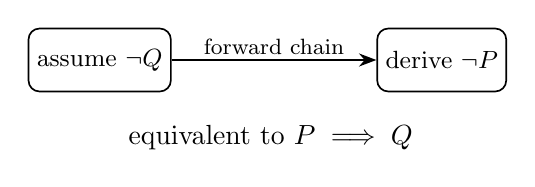
\begin{tikzpicture}[node distance=10mm]
  \node[procbox] (nQ) {assume $\lnot Q$};
  \node[procbox,right=26mm of nQ] (nP) {derive $\lnot P$};
  \node[draw=none,below=7mm of $(nQ)!0.5!(nP)$] (eq)
    {equivalent to $P\imp Q$};
  \path (nQ) edge[flow] node[flowlbl,above]{forward chain} (nP);
\end{tikzpicture}
\end{center}

\begin{wex}{Contrapositive: if $n^2$ is even then $n$ is even}
Prove for every integer $n$: if $n^2$ is even, then $n$ is even.
\wrec A direct attack would start from ``$n^2$ even'' and try to pry out a factor of $2$ from $n$ --
awkward, because square roots do not respect parity nicely. The negation ``$n$ is \emph{odd},'' by
contrast, is easy to compute with. A hypothesis that is hard to use but whose \emph{opposite
conclusion} is easy to manipulate is the trigger for the contrapositive.
\wsol The contrapositive is: if $n$ is odd, then $n^2$ is odd. Assume $n$ is odd, so $n=2k+1$ for
some integer $k$. Then
\[
  n^2=(2k+1)^2=4k^2+4k+1=2(2k^2+2k)+1,
\]
which is odd (one more than twice an integer). This proves the contrapositive, hence the original.
$\qquad\blacksquare$
\whichrule{The contrapositive is chosen because ``$n$ odd $\Rightarrow n^2$ odd'' is a direct
computation, whereas the original direction offers no algebraic foothold; and the two are logically
identical, so proving either settles the theorem.}
\emph{Check.} $n=5$ (odd): $n^2=25$ odd -- contrapositive instance holds. Original instance: $n^2=36$
even forces $n=\pm6$, even. Both consistent.
\end{wex}

\textbf{3. Proof by contradiction.} To prove a statement $S$, assume $\lnot S$ and derive a
contradiction (a statement and its own negation, or a known falsehood). Since $\lnot S$ leads to the
impossible, $S$ must hold. The flow branches into an assumption that is then detonated.
\begin{center}
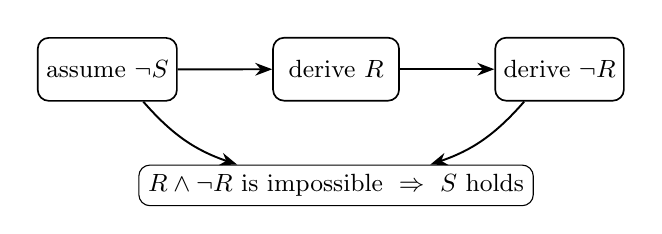
\begin{tikzpicture}[>=Stealth]
  \matrix (m) [matrix of math nodes, row sep=10mm, column sep=12mm,
    nodes={font=\small}]{
    |[procbox]| \text{assume }\lnot S &
    |[procbox]| \text{derive } R &
    |[procbox]| \text{derive }\lnot R\\
  };
  \node[draw,rounded corners,below=8mm of m-1-2,font=\small] (boom)
    {$R\land\lnot R$ is impossible $\;\Rightarrow\;$ $S$ holds};
  \path[->,line width=0.7pt]
    (m-1-1) edge (m-1-2)
    (m-1-2) edge (m-1-3);
  \path[->,line width=0.7pt] (m-1-1) edge[bend right=15] (boom);
  \path[->,line width=0.7pt] (m-1-3) edge[bend left=15] (boom);
\end{tikzpicture}
\end{center}

\begin{wex}{Contradiction: there is no largest prime}
Prove: there are infinitely many primes (equivalently, no integer is the largest prime).
\wrec The claim is an \emph{existence-forever} statement (``infinitely many''); negating it gives a
\emph{finite} list of all primes -- a concrete, manipulable object. Turning an unbounded claim into a
finite hypothesis you can compute against is the classic trigger for contradiction.
\wsol Suppose, for contradiction, that there are only finitely many primes, say all of them are
$p_1,p_2,\dots,p_k$. Consider
\[
  N=p_1p_2\cdots p_k+1.
\]
$N>1$, so $N$ has at least one prime divisor $p$. That $p$ must be one of the $p_i$ (they are all the
primes). But $p_i$ divides $p_1\cdots p_k$, so $p_i$ dividing $N$ would force $p_i$ to divide
$N-p_1\cdots p_k=1$ -- impossible, since no prime divides $1$. We have a prime divisor that both is
and is not on the list: a contradiction. Hence the primes are not finite. $\qquad\blacksquare$
\whichrule{Contradiction is the right tool when the statement denies existence of a bound or a
pattern: assuming the bound (a finite prime list) gives a finite object to compute with, and the
computed $N$ collides with the assumption.}
\emph{Check.} With the (false) list $\set{2,3,5}$, $N=2\cdot3\cdot5+1=31$, itself a prime not on the
list -- exactly the kind of escapee the argument guarantees.
\end{wex}

\textbf{4. Proof by construction.} To prove ``there exists an object with property $R$,'' build one
explicitly and verify it has $R$. The proof \emph{is} the recipe plus the check. This is the shape
that pervades automata theory: ``$\Lang$ is regular'' means ``here is a machine, and it works.''

\begin{wex}{Construction: a graph on any even $n\ge 4$ in which every vertex has degree $2$}
Prove: for every even integer $n\ge 4$ there is a graph with $n$ vertices in which every vertex has
degree exactly $2$.
\wrec ``There is a graph such that\dots'' is an \emph{existence} claim about a buildable object, so we
should display one and count degrees. A single cycle gives every vertex degree $2$ for free, and the
trigger ``exhibit an object with a uniform local property'' points straight at a regular,
symmetric construction.
\wsol Take the vertices $v_0,v_1,\dots,v_{n-1}$ and join consecutive vertices around a ring,
including the wrap-around edge $v_{n-1}v_0$. Formally the edge set is
$\set{\,\set{v_i,v_{i+1}} \st 0\le i\le n-2\,}\cup\set{\set{v_{n-1},v_0}}$. Each $v_i$ touches exactly
its two ring neighbours, so every vertex has degree $2$. Here is the construction for $n=6$:
\begin{center}
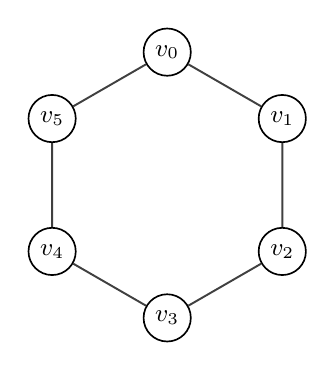
\begin{tikzpicture}[scale=1.25]
  \foreach \i in {0,...,5} {
    \node[gvlab] (v\i) at ({90-60*\i}:1.35cm) {$v_\i$};
  }
  \begin{scope}[on background layer]
    \foreach \i [evaluate=\i as \j using {int(mod(\i+1,6))}] in {0,...,5} {
      \draw[gedge] (v\i) -- (v\j);
    }
  \end{scope}
\end{tikzpicture}
\end{center}
The wrap-around edge $v_5v_0$ is present, so the figure is a single closed loop and degree $2$ is
uniform. (For $n$ even and $\ge 4$ the same ring works; evenness is not even needed for degree $2$,
but the claim was stated for even $n$, which the ring certainly covers.) $\qquad\blacksquare$
\whichrule{An existence claim is settled by \emph{exhibiting} a witness; the cycle on $n$ vertices is
the simplest object whose every vertex has the demanded degree, so building it and counting is the
whole proof.}
\emph{Check.} For $n=6$ the ring has $6$ edges; the degree sum is $2\cdot 6=12=\sum_v \deg v=6\cdot
2$, consistent with the handshake count.
\end{wex}

\textbf{5. Proof by cases.} When no single argument covers all inputs, split the domain into finitely
many exhaustive cases and prove the claim in each. The split must \emph{cover everything} (no gaps)
and ideally not overlap. The control flow is a fan-out followed by a join.
\begin{center}
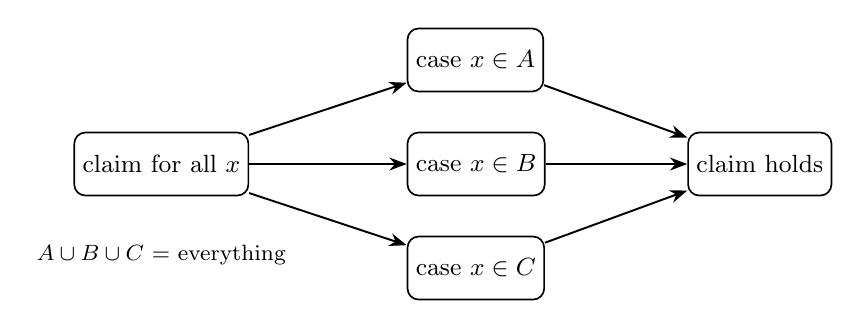
\begin{tikzpicture}[>=Stealth,node distance=9mm]
  \node[procbox] (all) {claim for all $x$};
  \node[procbox,above right=5mm and 20mm of all] (c1) {case $x\in A$};
  \node[procbox,right=20mm of all] (c2) {case $x\in B$};
  \node[procbox,below right=5mm and 20mm of all] (c3) {case $x\in C$};
  \node[procbox,right=18mm of c2] (done) {claim holds};
  \path (all) edge[flow] (c1) (all) edge[flow] (c2) (all) edge[flow] (c3)
        (c1) edge[flow] (done) (c2) edge[flow] (done) (c3) edge[flow] (done);
  \node[draw=none,below=5mm of all,font=\footnotesize] {$A\cup B\cup C$ = everything};
\end{tikzpicture}
\end{center}

\begin{wex}{Cases: $n^2+n$ is even for every integer $n$}
Prove: for every integer $n$, the number $n^2+n$ is even.
\wrec The quantity behaves differently depending on the parity of $n$, and ``every integer'' splits
cleanly into the two exhaustive cases \emph{even} and \emph{odd}. A property that hinges on a finite
classification of the input (here, parity) is the trigger for a case split.
\wsol Note $n^2+n=n(n+1)$, the product of two consecutive integers. Split on the parity of $n$.
\emph{Case 1: $n$ even.} Then $n=2k$, so $n(n+1)=2k(n+1)$ is twice an integer, hence even.
\emph{Case 2: $n$ odd.} Then $n+1$ is even, $n+1=2j$, so $n(n+1)=n\cdot 2j=2(nj)$ is even. Every
integer is even or odd and these are the only options, so the two cases are exhaustive and the claim
holds for all $n$. $\qquad\blacksquare$
\whichrule{Cases are forced here because the algebra ``which factor carries the $2$'' depends on the
parity of $n$; splitting on parity gives two exhaustive sub-claims, each a one-line direct argument.}
\emph{Check.} $n=3$ (odd): $n^2+n=12$, even, with the $2$ coming from $n+1=4$. $n=4$ (even):
$n^2+n=20$, even, with the $2$ coming from $n=4$.
\end{wex}

\subsection*{Equivalences and disproofs}

Two further patterns appear constantly. A \emph{biconditional} $P\eqv Q$ is proved by establishing
both implications separately; a \emph{set equality} $A=B$ is the same shape, proving $A\subseteq B$
and $B\subseteq A$.

\begin{wex}{A biconditional, proved in two directions}
Prove: an integer $n$ is divisible by $6$ \emph{iff} it is divisible by both $2$ and $3$.
\wrec The connective is ``iff,'' i.e.\ a biconditional $P\eqv Q$, which Definition~\ref{def:forms@c1}
says must be split into a forward and a reverse implication. The ``iff'' itself is the trigger.
\wsol \emph{($\Rightarrow$)} If $6\mid n$ then $n=6k=2(3k)=3(2k)$, so $2\mid n$ and $3\mid n$.
\emph{($\Leftarrow$)} Suppose $2\mid n$ and $3\mid n$. From $2\mid n$, write $n=2m$. Since $3\mid n=2m$
and $3$ shares no factor with $2$, we get $3\mid m$, say $m=3t$; then $n=2\cdot 3t=6t$, so $6\mid n$.
Both directions hold, so the biconditional is proved. $\qquad\blacksquare$
\whichrule{A biconditional is two theorems in one wrapper; each arrow is proved by its own short
direct argument, and only when \emph{both} are in hand is the ``iff'' established.}
\emph{Check.} $n=12$: divisible by $6$ and by both $2,3$ -- both sides true. $n=9$: not divisible by
$6$, and indeed not by $2$ -- both sides false, consistent.
\end{wex}

A \emph{universal} statement is disproved by a single \emph{counterexample}; you switch from proving
to refuting, and one bad instance suffices.

\begin{wex}{Disproof by counterexample}
Decide whether this is true: ``for every pair of primes $p,q$, the sum $p+q$ is even.''
\wrec The claim is universal (``for every pair''). To \emph{refute} a universal it is enough to
exhibit one pair where the conclusion fails -- a counterexample. Suspecting an edge case (the only
even prime) is the trigger.
\wsol The statement is false. Take $p=2$ and $q=3$, both prime; then $p+q=5$, which is odd. This
single pair violates the claim, so the universal statement is refuted. $\qquad\blacksquare$
\whichrule{One counterexample kills a ``for all'' claim, because the negation of ``for all $x$,
$R(x)$'' is ``there exists $x$ with $\lnot R(x)$,'' and the witness $x=(2,3)$ supplies exactly that.}
\emph{Check.} The claim is rescued by adding ``both odd'': for odd primes $p,q$ the sum is even
($\text{odd}+\text{odd}$), and the lone offender is the even prime $2$.
\end{wex}

The dependency between the methods is itself a small hierarchy: contrapositive and contradiction are
re-expressings of a direct argument over a negated statement, while biconditional and case proofs are
direct proofs assembled from smaller direct pieces. The Hasse-style picture below orders the methods
by ``builds on'':
\begin{center}
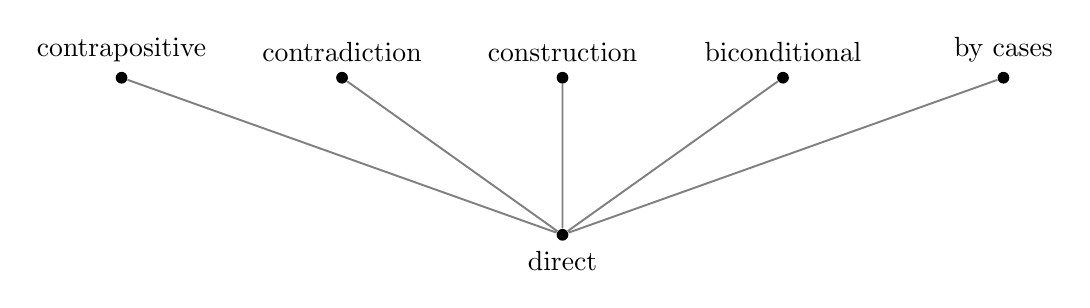
\begin{tikzpicture}[yscale=1.05]
  \node[ltdot,label=below:{direct}] (d) at (0,0) {};
  \node[ltdot,label=above:{contrapositive}] (cp) at (-5.6,1.9) {};
  \node[ltdot,label=above:{contradiction}] (cd) at (-2.8,1.9) {};
  \node[ltdot,label=above:{construction}] (co) at (0,1.9) {};
  \node[ltdot,label=above:{biconditional}] (bi) at (2.8,1.9) {};
  \node[ltdot,label=above:{by cases}] (ca) at (5.6,1.9) {};
  \draw[ltedge] (d)--(cp) (d)--(cd) (d)--(co) (d)--(bi) (d)--(ca);
\end{tikzpicture}
\end{center}
The point of the picture is practical: when a fancier method stalls, drop to the direct argument
underneath it and see what is really being claimed.

\begin{method}{How to pick a proof method from the statement's form}
\begin{enumerate}[leftmargin=2em,topsep=2pt,itemsep=1pt]
  \item \textbf{Read off the logical form} (Definition~\ref{def:forms@c1}): is it $P\imp Q$, $P\eqv Q$,
  ``for all,'' or ``there exists''? Rewrite it in those words before doing anything else.
  \item \textbf{Existence claim?} Try a \emph{construction}: build the object, then verify it has the
  property.
  \item \textbf{Universal claim you suspect is false?} Hunt for a \emph{counterexample}; one instance
  ends it.
  \item \textbf{Implication $P\imp Q$?} Default to a \emph{direct} proof. If $P$ is awkward but
  ``not $Q$'' is concrete, switch to the \emph{contrapositive}. If the statement denies a bound or an
  existence (``no largest\dots,'' ``infinitely many\dots''), reach for \emph{contradiction}.
  \item \textbf{Biconditional $P\eqv Q$ or set equality $A=B$?} Prove the two implications (two
  inclusions) separately.
  \item \textbf{Behaviour depends on a finite classification?} Split into exhaustive \emph{cases} and
  prove each; check that the cases leave no gap.
  \item \textbf{Always end with a check} on a small instance, and confirm you proved the statement,
  not its converse.
\end{enumerate}
\end{method}

\begin{pitfall}
Proving the \emph{converse} by accident. To prove $P\imp Q$ you may assume $P$ and must reach $Q$;
assuming $Q$ and reaching $P$ proves the unrelated statement $Q\imp P$. The contrapositive
$(\lnot Q)\imp(\lnot P)$ \emph{is} a legitimate substitute (it is equivalent), but the converse is
not. Whenever you finish, reread the first and last lines and make sure the hypothesis you assumed is
the one the theorem gave you.
\end{pitfall}

\begin{pitfall}
A case split that is not exhaustive proves nothing. If you argue ``$n$ even'' and ``$n$ divisible by
$3$'' as your two cases, you have left out odd $n$ not divisible by $3$ -- the cases do not cover the
domain, so the conclusion is unjustified. Always state explicitly why your cases together exhaust
every possibility (``every integer is even or odd, and these are the only options'').
\end{pitfall}

\begin{pitfall}
In a proof by contradiction, the contradiction must be a genuine logical impossibility ($R$ and
$\lnot R$, or a known falsehood like $3\mid 1$), not merely something surprising or ugly. Deriving a
strange-looking equation is not a contradiction unless it actually contradicts a fact you already
hold. State clearly which two incompatible things you have derived.
\end{pitfall}

\begin{exers}{Exercises.}
\item For each statement, name its logical form (implication, biconditional, universal, or
existential) and write out its negation in plain words.
  \begin{enumerate}[label=(\alph*),topsep=1pt,itemsep=1pt]
    \item For every string $w\in\set{0,1}\kstar$, the reversal $\rev{w}$ has the same length as $w$.
    \item There exists an integer that is both a perfect square and one more than a multiple of $3$.
    \item If a graph is a tree then it has no cycle.
  \end{enumerate}

\item Give a \emph{direct} proof: if $a$ and $b$ are odd integers, then $a+b$ is even. Then state
the contrapositive of ``if $a+b$ is odd then $a$ and $b$ are not both odd,'' and say whether it is
true.

\item Prove by \emph{contrapositive}: for every integer $n$, if $n^2$ is divisible by $3$ then $n$ is
divisible by $3$. (You may use the case split on the remainder of $n$ modulo $3$.)

\item Prove by \emph{contradiction} that $\sqrt{3}$ is irrational. State precisely which two
incompatible facts you derive at the end.

\item By \emph{construction}, prove that for every $n\ge 1$ there is a string over $\set{0,1}$ of
length $2n$ that is equal to its own reversal (a palindrome). Exhibit your string as a function of
$n$ and verify the palindrome property.

\item Prove by \emph{cases} that for every integer $n$, exactly one of $n$ and $n+1$ is even. Make
the exhaustiveness of your cases explicit.

\item Prove the biconditional: an integer $n$ is even \emph{iff} $n^2$ is even. Clearly separate the
forward and reverse directions and say which proof technique you use for each.

\item Disprove by \emph{counterexample}: ``for all integers $a,b,c$, if $a$ divides $bc$ then $a$
divides $b$ or $a$ divides $c$.'' Exhibit specific $a,b,c$ and explain why they refute the claim.

\item Find the error in the following ``proof.''
\emph{Claim.} If $x^2=y^2$ then $x=y$, for all real $x,y$.
\emph{Proof.} Assume $x^2=y^2$. Taking square roots of both sides gives $x=y$, as required.
Identify the false step and give a counterexample to the claim itself.

\item Find the error in the following case proof.
\emph{Claim.} Every integer $n$ satisfies $n^2\ge n$.
\emph{Proof.} \emph{Case $n\ge 1$:} multiplying $n\ge 1$ by the positive number $n$ gives $n^2\ge n$.
\emph{Case $n=0$:} $0\ge 0$. So $n^2\ge n$ for all integers $n$.
Explain which integers the cases fail to cover, and either repair the proof or give a value of $n$
where the claim is in fact still true but uncovered.

\item Let $P$ be ``$w$ ends in $\str0$'' and $Q$ be ``$w$ has even length,'' for strings
$w\in\set{0,1}\kstar$. Decide whether ``$P\imp Q$'' is true. If true, prove it; if false, give the
shortest counterexample $w$.

\item Consider the statement ``for every simple graph $G$ on $n\ge 2$ vertices, some two vertices of
$G$ have the same degree.'' Prove it by contradiction. (Hint: in a simple graph on $n$ vertices each
degree lies in $\set{0,1,\dots,n-1}$; argue that the values $0$ and $n-1$ cannot both occur, so only
$n-1$ distinct degree values are available for $n$ vertices.)
\end{exers}


\section{Induction and the Well-Ordering Principle}
Induction is the proof technique that lets a finite argument settle infinitely many cases at
once: prove a statement for a smallest object, then prove that the truth of the statement for
``smaller'' objects forces it for the next one up, and the statement holds for every object in
the family. The one key idea is that this works for \emph{any} collection whose members can be
built up from base cases by finitely many construction steps -- not just the natural numbers but
strings, trees, and the runs of an automaton. Because every machine we will study processes its
input one step at a time and every language we recognize is defined by a recursive grammar,
induction along the building-up order is the workhorse for proving machines correct; this section
isolates the principle in its three guises (weak, strong, and structural) and ties each to the
well-ordering principle that justifies them all.

\subsection*{The natural-number principles}

\begin{definition}[Well-ordering principle]\label{def:wop@c1}
The \emph{well-ordering principle} states: every nonempty subset $S\subseteq\N$ has a
\emph{least element}, that is, an $m\in S$ with $m\le n$ for all $n\in S$. (Here $\N=\set{0,1,2,\dots}$;
the same holds for $\set{1,2,\dots}$.)
\end{definition}

We take well-ordering as the basic fact about $\N$ and derive induction from it. The point of doing
so is that the two are logically equivalent, and seeing the equivalence explains \emph{why}
induction is allowed to conclude something about all of an infinite set from two finite proofs.

\begin{theorem}[Principle of mathematical induction, weak form]\label{thm:weakind@c1}
Let $P(n)$ be a statement about natural numbers $n\ge b$. Suppose
\begin{itemize}[leftmargin=2.2em,topsep=2pt,itemsep=1pt]
  \item \emph{(Basis)} $P(b)$ is true, and
  \item \emph{(Induction step)} for every $k\ge b$, if $P(k)$ is true then $P(k{+}1)$ is true.
\end{itemize}
Then $P(n)$ is true for every $n\ge b$.
\end{theorem}
\begin{proof}
Suppose not. Then the set $S=\set{n\ge b \st P(n)\text{ is false}}$ is nonempty, so by the
well-ordering principle (Definition~\ref{def:wop@c1}) it has a least element $m$. Since $P(b)$ holds,
$m\ne b$, so $m>b$ and hence $m-1\ge b$. By minimality of $m$, the number $m-1$ is \emph{not} in
$S$, so $P(m-1)$ is true. But the induction step applied at $k=m-1$ then makes $P(m)$ true,
contradicting $m\in S$. So $S=\es$ and $P(n)$ holds for all $n\ge b$.
\end{proof}

The induction step never claims $P(k)$ outright; it claims only the \emph{implication}
$P(k)\Rightarrow P(k{+}1)$. The temporary assumption $P(k)$ inside that proof is the
\emph{induction hypothesis}. A useful picture is a row of dominoes: the basis topples the first,
the induction step guarantees each domino topples its successor, and so the whole infinite row
falls. The chain of implications below makes the metaphor exact.

\begin{center}
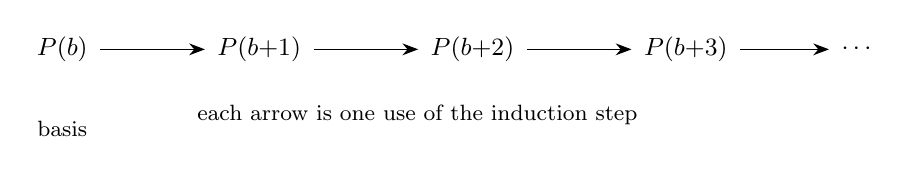
\begin{tikzpicture}[>={Stealth[length=2mm]},node distance=14mm,font=\small]
  \node (b) {$P(b)$};
  \node[right=of b] (k1) {$P(b{+}1)$};
  \node[right=of k1] (k2) {$P(b{+}2)$};
  \node[right=of k2] (k3) {$P(b{+}3)$};
  \node[right=12mm of k3] (dots) {$\cdots$};
  \path[->,shorten >=1pt,shorten <=1pt]
    (b) edge (k1) (k1) edge (k2) (k2) edge (k3) (k3) edge (dots);
  \node[below=5mm of b,font=\footnotesize] {basis};
  \node[below=3mm of k2,font=\footnotesize,xshift=-7mm] {each arrow is one use of the induction step};
\end{tikzpicture}
\end{center}

\begin{theorem}[Strong induction]\label{thm:strongind@c1}
Let $P(n)$ be a statement about $n\ge b$. Suppose that for every $k\ge b$,
\[
  \bigl(P(j)\text{ holds for all } b\le j<k\bigr)\ \Longrightarrow\ P(k).
\]
Then $P(n)$ holds for all $n\ge b$. (When $k=b$ the hypothesis is vacuous, so this single clause
already includes the basis $P(b)$.)
\end{theorem}
\begin{proof}
Again suppose the set $S=\set{n\ge b\st P(n)\text{ false}}$ is nonempty and let $m$ be its least
element. Every $j$ with $b\le j<m$ lies outside $S$ by minimality, so $P(j)$ holds for all such
$j$. The hypothesis at $k=m$ then yields $P(m)$, contradicting $m\in S$.
\end{proof}

Strong induction differs from the weak form only in the strength of the hypothesis: to prove
$P(k)$ you may assume $P(j)$ for \emph{all} earlier $j$, not just the immediate predecessor.
Logically the two are equivalent -- each proves the other -- but strong induction is the natural
choice when reaching $P(k)$ needs a value of $P$ that is more than one step back, such as a
recurrence that refers to $P(k-2)$, or a number that splits into two strictly smaller factors.

Both proofs above ran the same way: assume a counterexample, take the \emph{least} one, and derive
a contradiction from a still-smaller case. Well-ordering is exactly what forbids an infinite
strictly-decreasing chain of naturals -- any such chain would be a nonempty set with no least
element. The schematic below shows a descent of failing cases halted at the least bad case $m$;
the induction step proves that even $m$ cannot fail, so no bad case survives.

\begin{center}
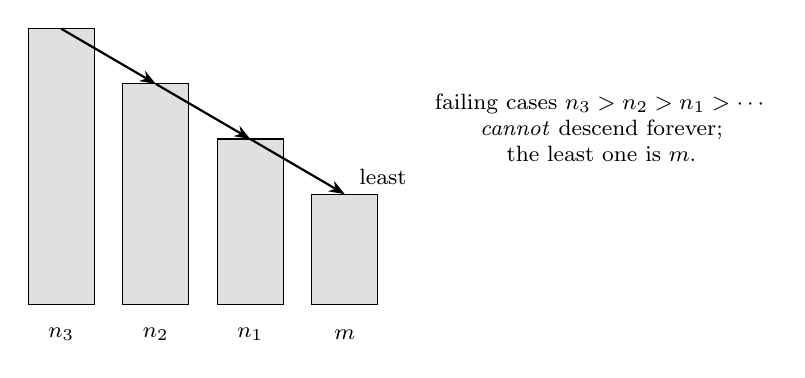
\begin{tikzpicture}[>={Stealth[length=2mm]},font=\small,x=12mm,y=7mm]
  \foreach \i/\h/\lab in {0/5/{n_3}, 1/4/{n_2}, 2/3/{n_1}, 3/2/{m}} {
    \fill[black!12] (\i,0) rectangle (\i+0.7,\h);
    \draw (\i,0) rectangle (\i+0.7,\h);
    \node[font=\footnotesize] at (\i+0.35,-0.55) {$\lab$};
  }
  \draw[->,thick] (0.35,5) -- (1.35,4);
  \draw[->,thick] (1.35,4) -- (2.35,3);
  \draw[->,thick] (2.35,3) -- (3.35,2);
  \node[font=\footnotesize,align=center,anchor=west] at (4.2,3.2)
    {failing cases $n_3>n_2>n_1>\cdots$\\ \emph{cannot} descend forever;\\
     the least one is $m$.};
  \node[font=\footnotesize,anchor=south west] at (3.4,2.0) {least};
\end{tikzpicture}
\end{center}

\begin{wex}{A summation by weak induction}
Prove that $\displaystyle\sum_{i=1}^{n} i=\frac{n(n{+}1)}{2}$ for every $n\ge 1$.
\wrec The claim is indexed by a single integer $n$ and the value at $n$ is obtained from the value
at $n-1$ by adding one term. ``Built from the previous case by one step'' is the trigger for
\emph{weak} induction.
\wsol Let $P(n)$ be the displayed equation.

\emph{Basis} ($n=1$): the left side is $1$ and the right side is $\frac{1\cdot 2}{2}=1$. So $P(1)$
holds.

\emph{Induction step:} fix $k\ge 1$ and assume $P(k)$, i.e.\ $\sum_{i=1}^{k}i=\frac{k(k+1)}{2}$.
Then
\[
  \sum_{i=1}^{k+1} i=\Bigl(\sum_{i=1}^{k} i\Bigr)+(k{+}1)
  \overset{P(k)}{=}\frac{k(k{+}1)}{2}+(k{+}1)
  =(k{+}1)\cdot\frac{k+2}{2}=\frac{(k{+}1)(k{+}2)}{2},
\]
which is exactly $P(k{+}1)$. By Theorem~\ref{thm:weakind@c1}, $P(n)$ holds for all $n\ge1$.
\whichrule{Weak induction fits because the inductive step uses the single immediately preceding
case $P(k)$ and nothing earlier; the new term $(k{+}1)$ is precisely the gap between consecutive
sums.}
\emph{Check.} At $n=4$: $1+2+3+4=10$ and $\frac{4\cdot 5}{2}=10$.
\end{wex}

\begin{wex}{A statement that genuinely needs strong induction}
Prove that every integer $n\ge 2$ is a product of one or more primes.
\wrec Factoring $n$ may split it as $n=ab$ with $a,b$ \emph{both} strictly between $1$ and $n$;
the conclusion for $n$ then rests on the conclusion for two numbers that can be far below $n-1$.
``The case $k$ depends on arbitrary smaller cases'' is the trigger for \emph{strong} induction.
\wsol Let $P(n)$ be ``$n$ is a product of primes.''

\emph{Step} (basis folded in): fix $k\ge 2$ and assume $P(j)$ for all $j$ with $2\le j<k$. Two
cases. If $k$ is prime, then $k$ is a one-factor product of primes and $P(k)$ holds outright (this
covers $k=2$, where the hypothesis is vacuous). If $k$ is composite, write $k=ab$ with
$2\le a,b<k$. By the induction hypothesis $P(a)$ and $P(b)$ both hold, so $a$ and $b$ are each
products of primes; concatenating those two factorizations expresses $k$ as a product of primes.
Either way $P(k)$ holds. By Theorem~\ref{thm:strongind@c1}, every $n\ge 2$ is a product of primes.
\begin{center}
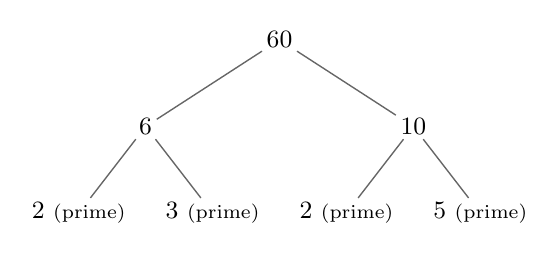
\begin{tikzpicture}[treenode,level distance=11mm,
   level/.style={sibling distance=34mm/#1},edge from parent/.style={tedge,draw}]
  \node {$60$}
    child {node {$6$}
      child {node {$2$ \scriptsize(prime)}}
      child {node {$3$ \scriptsize(prime)}}}
    child {node {$10$}
      child {node {$2$ \scriptsize(prime)}}
      child {node {$5$ \scriptsize(prime)}}};
\end{tikzpicture}
\end{center}
\whichrule{The split $k=ab$ can drop the problem to numbers nowhere near $k-1$ (here $60\to6,10$),
so only the \emph{strong} hypothesis -- all smaller cases available at once -- reaches them; the
recursion tree bottoms out at primes, which are the base case.}
\emph{Check.} The tree for $60$ multiplies back: $2\cdot3\cdot2\cdot5=60$, and every leaf is prime.
\end{wex}

\begin{wex}{A divide-and-conquer recurrence, by strong induction on a recursion tree}
Let $T(1)=0$ and, for $n$ a power of $2$ with $n\ge 2$, let $T(n)=2\,T(n/2)+n$. Prove
$T(n)=n\log_2 n$ for every $n=2^k$, $k\ge 0$.
\wrec The value $T(n)$ is defined from $T(n/2)$ -- an index a \emph{factor} of two below $n$, far
from $n-1$. A recurrence whose argument halves (or otherwise drops to a fraction of $n$) is the
signature of \emph{strong} induction, organized as a recursion tree where each node spawns two
half-size children.
\wsol Induct on $k$ where $n=2^k$, with $P(k)\colon T(2^k)=2^k\cdot k$. \emph{Basis} $k=0$: $n=1$ and
$T(1)=0=1\cdot 0$. \emph{Step}: assume $P(k)$, so $T(2^k)=2^k k$; then with $n=2^{k+1}$,
\[
  T(2^{k+1})=2\,T(2^{k})+2^{k+1}\overset{P(k)}{=}2\cdot 2^{k}k+2^{k+1}
  =2^{k+1}k+2^{k+1}=2^{k+1}(k+1),
\]
which is $P(k+1)$ since $\log_2 2^{k+1}=k+1$. The recursion tree below makes the total transparent:
the $+n$ work at a node of size $n$ sums to $n$ across each level, and there are $\log_2 n$ levels of
internal nodes, giving $n\log_2 n$.
\begin{center}
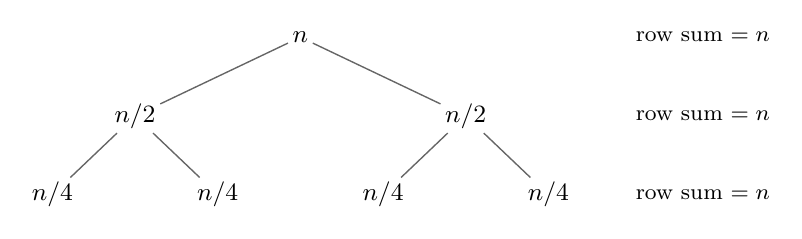
\begin{tikzpicture}[treenode,level distance=10mm,
   level/.style={sibling distance=42mm/#1},edge from parent/.style={tedge,draw}]
  \node {$n$}
    child {node {$n/2$}
      child {node {$n/4$}}
      child {node {$n/4$}}}
    child {node {$n/2$}
      child {node {$n/4$}}
      child {node {$n/4$}}};
  \node[anchor=west,font=\footnotesize,align=left] at (4.2,0)
    {row sum $=n$};
  \node[anchor=west,font=\footnotesize,align=left] at (4.2,-1.0)
    {row sum $=n$};
  \node[anchor=west,font=\footnotesize,align=left] at (4.2,-2.0)
    {row sum $=n$};
\end{tikzpicture}
\end{center}
\whichrule{Halving the argument places the recursive call at $n/2$, below $n-1$ once $n\ge 4$,
so weak induction on $n$ cannot reach it; strong induction on $n$ (equivalently, ordinary induction
on $k=\log_2 n$) supplies $T(n/2)$ directly, and the recursion tree reads off the $\log_2 n$ equal
rows that give $n\log_2 n$.}
\emph{Check.} $n=4$: $T(4)=2T(2)+4=2(2T(1)+2)+4=2\cdot 2+4=8=4\log_2 4$. The tree for $n=4$ has two
levels of internal nodes, matching $\log_2 4=2$.
\end{wex}

\begin{pitfall}
\textbf{No basis, no induction.} The induction step alone proves nothing: from
``$P(k)\Rightarrow P(k{+}1)$'' for all $k$ you can derive a true conclusion only after anchoring
some actual case. The bogus ``all horses are one color'' argument has a perfectly valid step
for $k\ge 2$ but silently uses an overlap of two sub-groups that fails at $k=1$, so the step from
$k=1$ to $k=2$ is the false link -- the basis does not connect to the rest.
\end{pitfall}

\subsection*{Structural induction}

The constructions we care about -- strings, well-formed expressions, parse trees, the runs of a
machine -- are defined \emph{recursively}: a few base objects, plus rules that build new objects
from old ones. For such families there is a tailored form of induction that mirrors the
definition exactly.

\begin{definition}[Inductively defined set]\label{def:inddef@c1}
A set $X$ is \emph{defined inductively} by giving (i) one or more \emph{base} elements that belong
to $X$, and (ii) one or more \emph{constructors}, each of which produces a new element of $X$ from
finitely many elements already known to be in $X$. The set $X$ is the \emph{smallest} collection
closed under these rules: $x\in X$ iff $x$ can be built from base elements by finitely many
applications of the constructors.
\end{definition}

\begin{theorem}[Structural induction]\label{thm:struct@c1}
Let $X$ be defined inductively as in Definition~\ref{def:inddef@c1}, and let $P$ be a property of
elements of $X$. If
\begin{itemize}[leftmargin=2.2em,topsep=2pt,itemsep=1pt]
  \item $P$ holds of every base element, and
  \item whenever a constructor builds $x$ from already-built pieces $x_1,\dots,x_r$, the truth of
  $P(x_1),\dots,P(x_r)$ forces $P(x)$,
\end{itemize}
then $P$ holds of every element of $X$.
\end{theorem}
\begin{proof}
Assign to each $x\in X$ its \emph{construction length} $\ell(x)$, the least number of constructor
applications needed to build $x$ from base elements (base elements have $\ell=0$). Then
$\ell(x)\in\N$, and we prove $Q(n)\colon$ ``$P(x)$ holds for every $x$ with $\ell(x)\le n$'' by
strong induction on $n$ (Theorem~\ref{thm:strongind@c1}). For the step, take any $x$ with
$\ell(x)=n$. If $n=0$, $x$ is a base element and $P(x)$ holds by the first hypothesis. Otherwise
$x$ is built by a constructor from pieces $x_1,\dots,x_r$, each of which has construction length
$<n$; the induction hypothesis gives $P(x_1),\dots,P(x_r)$, and the second hypothesis then yields
$P(x)$. So $Q(n)$ holds for all $n$, i.e.\ $P$ holds throughout $X$.
\end{proof}

Structural induction is thus strong induction in disguise, run along the construction order rather
than the numeric order. In practice you never compute $\ell(x)$; you simply check $P$ on the base
elements and check that each constructor \emph{preserves} $P$. The recursive definition of strings
is the example we will lean on constantly.

\begin{definition}[Strings, inductively]\label{def:strind@c1}
Fix an alphabet $\Sig$. The set $\Sigstar$ of strings is defined inductively by:
(base) the empty string $\eps\in\Sigstar$; (constructor) if $w\in\Sigstar$ and $a\in\Sig$ then the
string $wa$ (append $a$ on the right) is in $\Sigstar$. Length is defined along the same recursion
by $\abs{\eps}=0$ and $\abs{wa}=\abs{w}+1$.
\end{definition}

\begin{wex}{Length adds over concatenation, by structural induction on strings}
For all $x,y\in\Sigstar$ prove $\abs{xy}=\abs{x}+\abs{y}$.
\wrec Strings are built by appending one symbol at a time (Definition~\ref{def:strind@c1}), and the
claim is about every pair of strings. ``Property of all elements of a recursively defined set'' is
the trigger for \emph{structural} induction; we induct on the second string $y$, since
concatenation $xy$ grows on the right exactly as $y$ is built.
\wsol Fix $x$ and let $P(y)$ be the equation $\abs{xy}=\abs{x}+\abs{y}$.

\emph{Base} ($y=\eps$): $xy=x\eps=x$, so $\abs{xy}=\abs{x}=\abs{x}+0=\abs{x}+\abs{\eps}$.

\emph{Constructor} ($y=wa$ with $a\in\Sig$, assuming $P(w)$): by definition of concatenation
$x(wa)=(xw)a$, so using $\abs{ua}=\abs{u}+1$ twice and the hypothesis $\abs{xw}=\abs{x}+\abs{w}$,
\[
  \abs{x(wa)}=\abs{(xw)a}=\abs{xw}+1\overset{P(w)}{=}(\abs{x}+\abs{w})+1
  =\abs{x}+(\abs{w}+1)=\abs{x}+\abs{wa}.
\]
So $P(wa)$ holds. By Theorem~\ref{thm:struct@c1}, $P(y)$ holds for every $y\in\Sigstar$.
\begin{center}
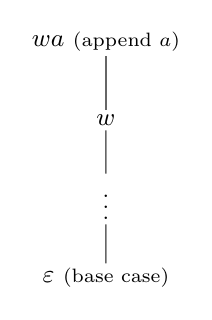
\begin{tikzpicture}[treenode,level distance=10mm,
   level/.style={sibling distance=46mm/#1},edge from parent/.style={tedge,draw}]
  \node {$wa$ \scriptsize(append $a$)}
    child {node {$w$}
      child {node[font=\footnotesize] {$\vdots$}
        child {node {$\eps$ \scriptsize(base case)}}}};
\end{tikzpicture}
\end{center}
\whichrule{Concatenation satisfies the recursion $x(wa)=(xw)a$ on its right argument, so structural
induction on $y$ lets each appended symbol contribute exactly $+1$ to both sides; the base $y=\eps$ is the only
non-recursive case, matching the single base clause of $\Sigstar$.}
\emph{Check.} With $x=\str{ab}$, $y=\str{cde}$: $\abs{xy}=\abs{\str{abcde}}=5$ and
$\abs{x}+\abs{y}=2+3=5$.
\end{wex}

\begin{wex}{Reversal is an anti-homomorphism: $\rev{(xy)}=\rev{y}\,\rev{x}$}
Define reversal by $\rev{\eps}=\eps$ and $\rev{(wa)}=a\,\rev{w}$ for $a\in\Sig$. Prove
$\rev{(xy)}=\rev{y}\,\rev{x}$ for all $x,y\in\Sigstar$.
\wrec Reversal is given recursively on a string's right end, so a claim about all $x,y$ asks for
structural induction; we again induct on $y$ because both $\rev{}$ and concatenation unfold by
recursion on the right ($\rev{(wa)}=a\,\rev{w}$ and $x(wa)=(xw)a$).
\wsol Fix $x$ and let $P(y)$ be $\rev{(xy)}=\rev{y}\,\rev{x}$.

\emph{Base} ($y=\eps$): $\rev{(x\eps)}=\rev{x}$, while $\rev{\eps}\,\rev{x}=\eps\,\rev{x}=\rev{x}$.
Equal.

\emph{Constructor} ($y=wa$, assuming $P(w)$): using $x(wa)=(xw)a$ and the defining rule
$\rev{(ua)}=a\,\rev{u}$,
\[
  \rev{(x(wa))}=\rev{((xw)a)}=a\,\rev{(xw)}
  \overset{P(w)}{=}a\,\rev{w}\,\rev{x}
  =\rev{(wa)}\,\rev{x},
\]
since $\rev{(wa)}=a\,\rev{w}$ by definition. So $P(wa)$ holds, and structural induction finishes.
\whichrule{The recursive clause $\rev{(wa)}=a\rev{w}$ peels the symbol off the right of $y$ and
plants it on the \emph{left} of the result, which is exactly why the two factors swap order;
induction on $y$ tracks that one symbol per step.}
\emph{Check.} $x=\str{ab},y=\str{cd}$: $\rev{(\str{abcd})}=\str{dcba}$ and
$\rev{\str{cd}}\,\rev{\str{ab}}=\str{dc}\cdot\str{ba}=\str{dcba}$.
\end{wex}

\begin{wex}{Counting the nodes of a full binary tree, structurally}
Define \emph{full binary trees} inductively: a single \emph{leaf} is a full binary tree; and if
$T_L,T_R$ are full binary trees then the tree with a new root joined to $T_L$ and $T_R$ is a full
binary tree. Prove that a full binary tree with $\ell$ leaves has exactly $\ell-1$ internal
(non-leaf) nodes.
\wrec The trees are a recursively defined family with one base (a leaf) and one two-piece
constructor (a root over $T_L,T_R$); a count over all such trees is structural induction on the
tree, with the hypothesis used on \emph{both} subtrees.
\wsol Let $i(T)$ and $\ell(T)$ be the numbers of internal nodes and leaves of $T$, and let $P(T)$
be ``$i(T)=\ell(T)-1$.''

\emph{Base} (a single leaf): $\ell=1$, $i=0$, and $0=1-1$. So $P$ holds.

\emph{Constructor} ($T$ = root over $T_L,T_R$, assuming $P(T_L)$ and $P(T_R)$): a leaf of $T$ is a
leaf of $T_L$ or of $T_R$, so $\ell(T)=\ell(T_L)+\ell(T_R)$; the internal nodes of $T$ are the new
root plus the internal nodes of each subtree, so $i(T)=1+i(T_L)+i(T_R)$. Then
\[
  i(T)=1+i(T_L)+i(T_R)\overset{\text{hyp}}{=}1+(\ell(T_L){-}1)+(\ell(T_R){-}1)
  =\bigl(\ell(T_L)+\ell(T_R)\bigr)-1=\ell(T)-1.
\]
So $P(T)$ holds, and Theorem~\ref{thm:struct@c1} gives the claim for all full binary trees.
\begin{center}
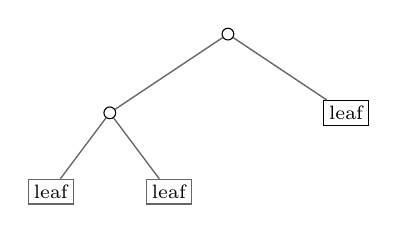
\begin{tikzpicture}[treenode,level distance=10mm,
   level/.style={sibling distance=30mm/#1},edge from parent/.style={tedge,draw}]
  \node[circle,draw,inner sep=1.5pt] {}
    child {node[circle,draw,inner sep=1.5pt] {}
      child {node[draw,rectangle,inner sep=2pt] {\scriptsize leaf}}
      child {node[draw,rectangle,inner sep=2pt] {\scriptsize leaf}}}
    child {node[draw,rectangle,inner sep=2pt] {\scriptsize leaf}};
\end{tikzpicture}
\end{center}
\whichrule{One base case and a constructor taking \emph{two} prior objects mean structural
induction must invoke the hypothesis on both $T_L$ and $T_R$ at once; the round nodes count toward
$i$ and the square leaves toward $\ell$, and the bookkeeping $\ell=i+1$ is preserved by adding one
root over two valid subtrees.}
\emph{Check.} The drawn tree has $3$ leaves and $2$ round internal nodes, and $2=3-1$.
\end{wex}

\begin{method}{How to run an induction proof}
\begin{enumerate}[leftmargin=2em,topsep=2pt,itemsep=1pt]
  \item \textbf{Name the variable you induct on} and state $P(\cdot)$ as a precise statement with
  that one variable free. For structural induction, name the recursively defined set and induct
  along its construction.
  \item \textbf{Choose the form.} If $P(k)$ follows from $P(k{-}1)$ alone, use weak induction
  (Theorem~\ref{thm:weakind@c1}). If it needs smaller cases that may be far back, or the object splits
  into smaller pieces, use strong (Theorem~\ref{thm:strongind@c1}) or structural
  (Theorem~\ref{thm:struct@c1}) induction.
  \item \textbf{Prove the basis} -- every base case. List them explicitly; a recursively defined
  set with two base elements needs both.
  \item \textbf{Prove the step.} Write down the induction hypothesis verbatim, then derive $P$ of
  the next object using \emph{only} the hypothesis and the definitions. Mark where you use the
  hypothesis (the $\overset{\text{hyp}}{=}$ tag above).
  \item \textbf{Confirm coverage.} Check that every element of the family is reached: every $n\ge b$
  for numeric induction, every object reachable by the constructors for structural induction.
\end{enumerate}
\end{method}

\begin{pitfall}
\textbf{Inducting on the wrong end of a recursive definition.} Strings in
Definition~\ref{def:strind@c1} are built by appending on the \emph{right}. If you try to prove a fact
about $\rev{}$ or concatenation by ``peeling a symbol off the left,'' you are using a different
recursion than the one the definitions follow, and the algebra will not line up. Match the
induction to the constructor: append-on-the-right definitions call for the constructor case
$y=wa$, not $y=aw$.
\end{pitfall}

\begin{pitfall}
\textbf{A too-weak hypothesis.} When a proof of $P(k)$ secretly uses $P(k{-}2)$ or $P(\lfloor
k/2\rfloor)$, weak induction's hypothesis (only $P(k{-}1)$) is not enough, and the step is invalid
even though it ``feels'' inductive. Switch to strong induction so the earlier cases are available.
Conversely, do not over-assume: the hypothesis covers cases \emph{strictly} smaller than the one
you are proving, never the case itself.
\end{pitfall}

\begin{exers}{Exercises.}
\item Prove by weak induction that $\sum_{i=1}^{n} i^2=\dfrac{n(n+1)(2n+1)}{6}$ for every
$n\ge 1$. State the induction hypothesis explicitly and mark where you use it.

\item Prove that $\sum_{i=1}^{n} (2i-1)=n^2$ for all $n\ge 1$ (the sum of the first $n$ odd numbers).
Then give a one-sentence geometric reason, in terms of building an $n\times n$ square one L-shaped
border at a time.

\item Prove by induction that $n^3-n$ is divisible by $6$ for every $n\ge 0$. (In the step, factor
$ (n+1)^3-(n+1)$ so the induction hypothesis appears.)

\item Prove that $2^n > n^2$ for every integer $n\ge 5$. Identify the smallest base value for which
the claim is true and explain why starting the basis any lower would break the induction.

\item Using only $4$-cent and $7$-cent stamps, prove that every postage amount of $n\ge 18$ cents
can be formed exactly. Decide how many base cases your strong induction needs and justify the number
in terms of how far back the inductive step reaches.

\item Define a sequence by $f_0=0$, $f_1=1$, and $f_{n}=f_{n-1}+f_{n-2}$ for $n\ge 2$. Prove by
strong induction that $f_n<2^n$ for all $n\ge 0$. Explain in one sentence why weak induction (using
only $f_{n-1}$) is insufficient here.

\item The well-ordering principle. Prove, using a least-counterexample argument, that every integer
$n\ge 2$ can be written as a product of primes. Then state precisely which step of your proof would
fail if $\N$ were replaced by the nonnegative rationals $\Q_{\ge 0}$, which are \emph{not}
well-ordered.

\item Strings are defined inductively by ``$\eps\in\Sigstar$; and if $w\in\Sigstar$, $a\in\Sig$ then
$wa\in\Sigstar$,'' with $\abs{\eps}=0$ and $\abs{wa}=\abs{w}+1$. Prove by structural induction on $y$
that $\abs{xy}=\abs{x}+\abs{y}$ for all $x,y\in\Sigstar$. State the constructor case you induct on.

\item Define the number of occurrences of a symbol $a$ in a string by $\#_a(\eps)=0$ and
$\#_a(wb)=\#_a(w)+[b=a]$ (where $[b=a]$ is $1$ if $b=a$ and $0$ otherwise). Prove by structural
induction that $\#_a(xy)=\#_a(x)+\#_a(y)$ for all strings $x,y$.

\item Reversal is defined by $\rev{\eps}=\eps$ and $\rev{(wa)}=a\,\rev{w}$. Prove by structural
induction that $\rev{(\rev{w})}=w$ for every $w\in\Sigstar$. (You may use, with a citation, the
identity $\rev{(xy)}=\rev{y}\,\rev{x}$.)

\item A full binary tree is a leaf, or a root joined to two full binary trees. Prove by structural
induction that a full binary tree with $i$ internal nodes has exactly $2i+1$ nodes in total. Draw a
small tree with $i=2$ and confirm your formula on it.

\item Let the height of a full binary tree be $h(\text{leaf})=0$ and
$h(\text{root over }T_L,T_R)=1+\max\set{h(T_L),h(T_R)}$, and let $\ell(T)$ be its leaf count. Prove
by structural induction that $\ell(T)\le 2^{\,h(T)}$ for every full binary tree $T$.

\item \emph{Find the bug.} A student ``proves'' that every finite set of lines in the plane, no two
parallel, passes through a single common point: ``Basis: one line trivially passes through a point on
it. Step: given $k+1$ such lines, by the hypothesis the first $k$ meet at a point $p$ and the last
$k$ meet at a point $q$; since both groups share the middle $k-1$ lines, $p=q$, so all $k+1$ lines
pass through $p$.'' Identify the smallest $k$ at which the step fails and explain why, in the spirit
of the ``all horses are the same color'' fallacy.

\item \emph{Find the bug.} Someone claims to prove $\abs{xy}=\abs{x}+\abs{y}$ by inducting on $x$
written as $x=a\,w$ (peel a symbol off the \emph{left}), with base case $x=\eps$. Explain why this
induction does not match the recursive definition of $\Sigstar$ given above, and state the change
needed to make the proof legitimate.
\end{exers}


% ================= Chapter 2: Graph Theory for Computation =================

\chapter{Graph Theory for Computation}

\section{Graphs, Digraphs, and Degrees}
A graph is the bare mathematics of ``things and the pairs of them that are related'': a finite set
of points together with a record of which points are joined. This is the data structure underneath
almost everything later in the book -- a finite automaton is a labelled graph, a computation is a
walk through a graph of configurations, and many of our hardest problems ($\HAMPATH$, $\CLIQUE$,
coloring) are questions about graphs. The one key idea of this section is that local information --
how many edges touch each vertex -- already constrains the global object rigidly, and the
\emph{handshake lemma} is our first proof of that. We make graphs and directed graphs precise,
define adjacency and degree, prove the handshake lemma and its parity corollary, and then read
those numbers off many small drawn examples.

\begin{definition}[Simple graph]\label{def:graph@c2}
A \emph{(simple, undirected) graph} is a pair $\Gr=(\Vset,\Eset)$ where $\Vset$ is a finite set of
\emph{vertices} and $\Eset$ is a set of \emph{edges}, each edge being a two-element subset
$\set{u,v}\subseteq\Vset$ with $u\ne v$. We write an edge $\set{u,v}$ as $uv$ (so $uv=vu$). Two
vertices $u,v$ are \emph{adjacent} if $uv\in\Eset$, and then each is \emph{incident} with the edge
$uv$. The word \emph{simple} encodes two bans: no edge from a vertex to itself (no \emph{loops},
since $u\ne v$), and no two parallel copies of the same edge (since $\Eset$ is a \emph{set}).
\end{definition}

Because each edge is an unordered pair, a graph on $n=\card{\Vset}$ vertices can have at most
$\binom{n}{2}=\tfrac{n(n-1)}{2}$ edges; the graph attaining this maximum, in which every pair is
joined, is the \emph{complete graph} $K_n$. The next definition packages the local picture at a
single vertex.

\begin{definition}[Neighborhood and degree]\label{def:degree@c2}
Let $\Gr=(\Vset,\Eset)$ and $v\in\Vset$. The \emph{neighborhood} of $v$ is the set of vertices
adjacent to it,
\[
  N(v)=\set{\,u\in\Vset \st uv\in\Eset\,},
\]
and the \emph{degree} of $v$ is $\deg(v)=\card{N(v)}$, the number of edges incident with $v$.
A vertex of degree $0$ is \emph{isolated}; a vertex of degree $1$ is a \emph{leaf} (or pendant).
The \emph{degree sequence} of $\Gr$ is the list of all vertex degrees written in nonincreasing
order.
\end{definition}

In a simple graph $\deg(v)$ counts neighbors and incident edges interchangeably, since each incident
edge supplies exactly one distinct neighbor. (Once loops or parallel edges are allowed the two
counts diverge, which is one reason we insist on ``simple'' as the default.) The most useful fact
about degrees is that, summed over the whole graph, they cannot be arbitrary.

\begin{theorem}[Handshake lemma]\label{thm:handshake@c2}
For every graph $\Gr=(\Vset,\Eset)$,
\[
  \sum_{v\in\Vset}\deg(v)=2\card{\Eset}.
\]
\end{theorem}

\begin{proof}
Count, in two ways, the number of \emph{incidences} -- pairs $(v,e)$ where $v$ is a vertex, $e$ is an
edge, and $v$ is an endpoint of $e$. Grouping the incidences by their vertex, each vertex $v$ lies in
exactly $\deg(v)$ incidences, so the total is $\sum_{v}\deg(v)$. Grouping instead by their edge, each
edge $e=uv$ has exactly two endpoints and so contributes exactly two incidences, giving the total
$2\card{\Eset}$. The two counts are of the same set, hence equal.
\end{proof}

\begin{corollary}[Parity of odd-degree vertices]\label{cor:parity@c2}
In every graph the number of vertices of odd degree is even.
\end{corollary}

\begin{proof}
Split the degree sum by parity. The vertices of even degree contribute an even total. By
Theorem~\ref{thm:handshake@c2} the grand total $\sum_v\deg(v)=2\card{\Eset}$ is even, so the
contribution of the odd-degree vertices is even as well. A sum of odd numbers is even only when there
is an even number of them; hence the odd-degree vertices number evenly.
\end{proof}

\begin{definition}[Directed graph]\label{def:digraph@c2}
A \emph{directed graph} (or \emph{digraph}) is a pair $\Gr=(\Vset,\Eset)$ where $\Eset\subseteq
\Vset\times\Vset$ is a set of \emph{ordered} pairs, the \emph{arcs}. An arc $(u,v)$, drawn as an
arrow $u\to v$, has \emph{tail} $u$ and \emph{head} $v$. The \emph{out-degree} $d^{+}(v)$ is the
number of arcs with tail $v$, and the \emph{in-degree} $d^{-}(v)$ is the number with head $v$. Here
$(u,v)$ and $(v,u)$ are distinct arcs, and (unless we say otherwise) self-arcs $(v,v)$ are allowed.
\end{definition}

Digraphs are the right model whenever a relation is one-directional: a transition $\trans(q,a)=q'$ of
a finite automaton is an arc $q\to q'$, and ``$x$ depends on $y$'' or ``$x$ reduces to $y$'' are
arcs. The handshake count has a directed analogue, separated by orientation.

\begin{proposition}[Directed handshake]\label{prop:dirhandshake@c2}
For every digraph $\Gr=(\Vset,\Eset)$,
$\displaystyle\sum_{v\in\Vset}d^{+}(v)=\sum_{v\in\Vset}d^{-}(v)=\card{\Eset}.$
\end{proposition}

\begin{proof}
Each arc $(u,v)$ has exactly one tail, so summing out-degrees counts every arc once:
$\sum_v d^{+}(v)=\card{\Eset}$. Likewise each arc has exactly one head, so $\sum_v
d^{-}(v)=\card{\Eset}$. The two sums equal the same number $\card{\Eset}$, hence each other.
\end{proof}

\textbf{Two ways to see a graph.} A graph is drawn as a \emph{diagram} -- a dot per vertex, a line per
edge, with no meaning attached to where the dots sit or whether the lines cross -- or recorded
combinatorially by listing $\Vset$ and $\Eset$. The drawing exposes structure to the eye; the lists
make ``which pairs are joined'' unambiguous. Only the \emph{incidence pattern} is the graph; two very
different-looking pictures can be the same graph, a fact we pin down with isomorphism.

\begin{definition}[Subgraph and induced subgraph]\label{def:subgraph@c2}
A graph $H=(\Vset_H,\Eset_H)$ is a \emph{subgraph} of $\Gr=(\Vset,\Eset)$, written $H\subseteq\Gr$,
if $\Vset_H\subseteq\Vset$ and $\Eset_H\subseteq\Eset$ (every retained edge must still join two
retained vertices). It is a \emph{spanning} subgraph if $\Vset_H=\Vset$. For $X\subseteq\Vset$, the
\emph{induced subgraph} $\Gr[X]$ has vertex set $X$ and \emph{all} edges of $\Gr$ with both endpoints
in $X$:
\[
  \Gr[X]=\bigl(X,\ \set{\,uv\in\Eset \st u,v\in X\,}\bigr).
\]
\end{definition}

A general subgraph may drop both vertices and edges freely; an induced subgraph chooses only which
vertices to keep and is then \emph{forced} to keep every original edge among them. So $\Gr[X]$ is the
densest subgraph on the vertex set $X$, and a subgraph $H$ on the same vertices is induced exactly
when it omits no available edge.

\begin{definition}[Isomorphism]\label{def:iso@c2}
Graphs $\Gr=(\Vset,\Eset)$ and $\Gr'=(\Vset',\Eset')$ are \emph{isomorphic}, written
$\Gr\cong\Gr'$, if there is a bijection $\varphi\colon\Vset\to\Vset'$ that preserves adjacency in both
directions:
\[
  uv\in\Eset \iff \varphi(u)\varphi(v)\in\Eset' \qquad\text{for all }u,v\in\Vset.
\]
Such a $\varphi$ is an \emph{isomorphism}. Isomorphic graphs are ``the same graph with relabelled
vertices.''
\end{definition}

An isomorphism must carry degrees to equal degrees -- if $\varphi(u)=u'$ then $u$ and $u'$ have the
same neighbors up to relabelling, so $\deg(u)=\deg(u')$. Hence the degree sequence is an
\emph{invariant}: graphs with different degree sequences cannot be isomorphic. (The converse fails;
matching degree sequences do not guarantee isomorphism, as Worked Example~\ref{wex:degseq@c2} shows.)

\begin{wex}{Reading degrees off a drawing, and checking the handshake lemma}
For the graph $\Gr$ with $\Vset=\set{a,b,c,d,e}$ and
$\Eset=\set{ab,ac,ad,bc,ce,de}$, list the degree of every vertex, give the degree sequence, and
verify Theorem~\ref{thm:handshake@c2}.
\wrec This is direct bookkeeping: degree is the count of incident edges, and the handshake lemma is
the cross-check that $\sum_v\deg(v)=2\card{\Eset}$. The trigger ``verify the lemma'' means compute
both sides independently and compare.
\wsol Draw the five vertices and the six edges, then count the lines meeting each dot.
\begin{center}
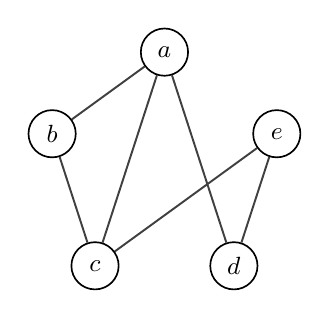
\begin{tikzpicture}[scale=1.5]
  \node[gvlab] (a) at (90:1) {$a$};
  \node[gvlab] (b) at (162:1) {$b$};
  \node[gvlab] (c) at (234:1) {$c$};
  \node[gvlab] (d) at (306:1) {$d$};
  \node[gvlab] (e) at (18:1) {$e$};
  \begin{scope}[on background layer]
    \draw[gedge] (a)--(b) (a)--(c) (a)--(d) (b)--(c) (c)--(e) (d)--(e);
  \end{scope}
\end{tikzpicture}
\end{center}
Counting incident edges: $\deg(a)=3$ (to $b,c,d$), $\deg(b)=2$ (to $a,c$), $\deg(c)=3$ (to
$a,b,e$), $\deg(d)=2$ (to $a,e$), $\deg(e)=2$ (to $c,d$). The degree sequence, sorted, is
$(3,3,2,2,2)$.
\whichrule{Degree is purely local -- count the lines at each dot -- and the handshake lemma equates
that local data, summed, with twice the (global) edge count; computing both sides is the verification
itself.}
\emph{Check.} $\sum_v\deg(v)=3+2+3+2+2=12$, and $2\card{\Eset}=2\cdot 6=12$. They agree, and the two
odd-degree vertices $a,c$ are even in number, consistent with Corollary~\ref{cor:parity@c2}.
\end{wex}

\begin{wex}{Counting edges of $K_n$ from degrees}
Use the handshake lemma to find the number of edges of the complete graph $K_n$ (every pair of
$n$ vertices joined), and confirm it on $K_5$.
\wrec A counting question where every degree is \emph{known} by symmetry but the edge count is not
yet. The trigger ``all degrees equal, edges wanted'' is exactly the situation the handshake lemma
turns around: it lets you solve for $\card{\Eset}$ from the degree sum.
\wsol In $K_n$ each vertex is adjacent to the other $n-1$ vertices, so $\deg(v)=n-1$ for all $v$.
The degree sum is therefore $n(n-1)$, and Theorem~\ref{thm:handshake@c2} gives
$2\card{\Eset}=n(n-1)$, hence
\[
  \card{\Eset}=\frac{n(n-1)}{2}=\binom{n}{2}.
\]
For $K_5$ this predicts $\binom{5}{2}=10$ edges, each vertex having degree $4$.
\begin{center}
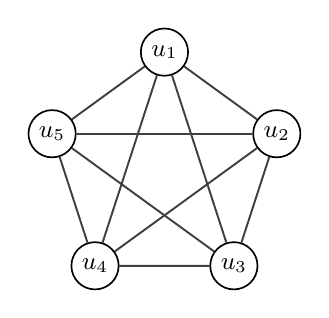
\begin{tikzpicture}[scale=1.5]
  \foreach \i/\name in {0/u_1,1/u_2,2/u_3,3/u_4,4/u_5} {
    \node[gvlab] (\i) at ({90-72*\i}:1) {$\name$};
  }
  \begin{scope}[on background layer]
    \foreach \i in {0,...,4} {
      \foreach \j in {0,...,4} {
        \ifnum\i<\j \draw[gedge] (\i)--(\j); \fi
      }
    }
  \end{scope}
\end{tikzpicture}
\end{center}
\whichrule{When every degree is forced by symmetry, the handshake lemma converts the easy degree sum
into the wanted edge count -- you never list the edges, you divide the degree sum by two.}
\emph{Check.} The drawing of $K_5$ has $\binom{5}{2}=10$ edges, and reading any single vertex shows
$4$ lines leaving it, so $\deg=4$ and $\sum_v\deg(v)=5\cdot4=20=2\cdot10$.
\end{wex}

\begin{wex}{In-degree and out-degree in a digraph}
Let the digraph $D$ have vertices $\set{p,q,r,s}$ and arcs $p\to q,\ q\to r,\ r\to p,\ q\to s,\ s\to
r$. Tabulate $d^{+}(v)$ and $d^{-}(v)$ for every vertex and verify
Proposition~\ref{prop:dirhandshake@c2}.
\wrec A digraph degree count: out-degree counts arrows \emph{leaving}, in-degree counts arrows
\emph{arriving}, and they are tracked separately. The trigger ``verify the directed handshake'' means
both sums must equal the number of arcs.
\wsol Draw each arc as an arrow from tail to head, then at each vertex count outgoing and incoming
arrowheads.
\begin{center}
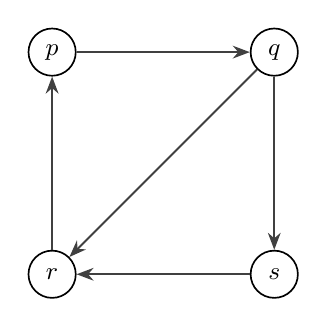
\begin{tikzpicture}[>=Stealth,node distance=22mm]
  \node[gvlab] (p) {$p$};
  \node[gvlab,right=of p] (q) {$q$};
  \node[gvlab,below=of q] (s) {$s$};
  \node[gvlab,below=of p] (r) {$r$};
  \draw[gedge,->] (p)--(q);
  \draw[gedge,->] (q)--(r);
  \draw[gedge,->] (r)--(p);
  \draw[gedge,->] (q)--(s);
  \draw[gedge,->] (s)--(r);
\end{tikzpicture}
\end{center}
\[
\begin{array}{c|cccc|c}
 v & p & q & r & s & \text{sum}\\\hline
 d^{+}(v) & 1 & 2 & 1 & 1 & 5\\
 d^{-}(v) & 1 & 1 & 2 & 1 & 5
\end{array}
\]
\whichrule{In a digraph the two degree notions are genuinely different per vertex (here $q$ has
$d^{+}=2,d^{-}=1$), but each arc has exactly one tail and one head, so both rows must total the
arc count.}
\emph{Check.} There are $5$ arcs; both $\sum_v d^{+}(v)$ and $\sum_v d^{-}(v)$ equal $5=\card{\Eset}$,
as the proposition requires. Note $d^{+}(q)\ne d^{-}(q)$, so the equality of the two sums does not
hold vertex by vertex.
\end{wex}

\begin{wex}{Subgraph versus induced subgraph}
Take $\Gr$ on $\Vset=\set{1,2,3,4}$ with $\Eset=\set{12,23,34,41,13}$ (a $4$-cycle plus the diagonal
$13$). For $X=\set{1,2,3}$, draw the induced subgraph $\Gr[X]$, and separately exhibit a subgraph on
$X$ that is \emph{not} induced.
\wrec The trigger is the contrast ``induced versus general.'' Induced is determined the instant you
pick $X$ -- keep every original edge inside $X$; a non-induced subgraph on the same vertices must
\emph{drop} at least one available edge.
\wsol Inside $X=\set{1,2,3}$ the original edges are $12,23$, and $13$ (the edges $34$ and $41$ leave
$X$, so they are gone). The induced subgraph keeps all three, forming a triangle:
\begin{center}
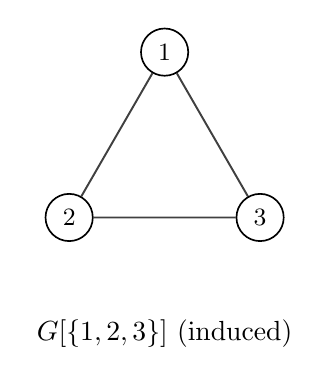
\begin{tikzpicture}[scale=1.4]
  \node[gvlab] (1) at (90:1) {$1$};
  \node[gvlab] (2) at (210:1) {$2$};
  \node[gvlab] (3) at (330:1) {$3$};
  \begin{scope}[on background layer]
    \draw[gedge] (1)--(2) (2)--(3) (1)--(3);
  \end{scope}
  \node at (0,-1.55) {$\Gr[\set{1,2,3}]$ (induced)};
\end{tikzpicture}
\qquad
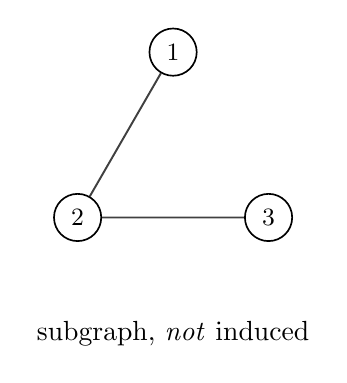
\begin{tikzpicture}[scale=1.4]
  \node[gvlab] (1) at (90:1) {$1$};
  \node[gvlab] (2) at (210:1) {$2$};
  \node[gvlab] (3) at (330:1) {$3$};
  \begin{scope}[on background layer]
    \draw[gedge] (1)--(2) (2)--(3);
  \end{scope}
  \node at (0,-1.55) {subgraph, \emph{not} induced};
\end{tikzpicture}
\end{center}
The right picture has the same three vertices but omits the available edge $13$, so it is a perfectly
good subgraph yet not the induced one.
\whichrule{Picking $X$ fixes the induced subgraph uniquely (all internal edges retained); any
subgraph on $X$ that discards an internal edge -- here $13$ -- is non-induced by definition.}
\emph{Check.} $\Gr[X]$ has $3$ edges (a triangle, degree sequence $(2,2,2)$); the non-induced example
has $2$ edges (a path, degree sequence $(2,1,1)$). Different edge counts on the same vertices confirm
they differ.
\end{wex}

\begin{wex}{Two drawings of one graph: building an isomorphism}
Show that the $4$-cycle drawn as a square is isomorphic to the same graph drawn as a ``crossed''
figure, by exhibiting an explicit vertex bijection.
\wrec ``Show isomorphic'' is a \emph{construction} task: produce a bijection and check it preserves
edges both ways. The trigger is that the drawings look different but we suspect identical incidence
structure, so a relabelling should match them.
\wsol Let $\Gr$ be the square with vertices $1,2,3,4$ and edges $12,23,34,41$. Let $\Gr'$ have
vertices $w,x,y,z$ and the \emph{same cyclic} adjacency but drawn with two edges crossing: edges
$wx,xy,yz,zw$. Define $\varphi(1)=w,\ \varphi(2)=x,\ \varphi(3)=y,\ \varphi(4)=z$.
\begin{center}
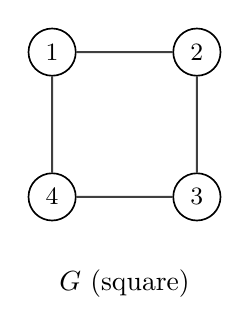
\begin{tikzpicture}[scale=1.3]
  \node[gvlab] (1) at (135:1) {$1$};
  \node[gvlab] (2) at (45:1) {$2$};
  \node[gvlab] (3) at (-45:1) {$3$};
  \node[gvlab] (4) at (-135:1) {$4$};
  \begin{scope}[on background layer]
    \draw[gedge] (1)--(2) (2)--(3) (3)--(4) (4)--(1);
  \end{scope}
  \node at (0,-1.55) {$\Gr$ (square)};
\end{tikzpicture}
\qquad
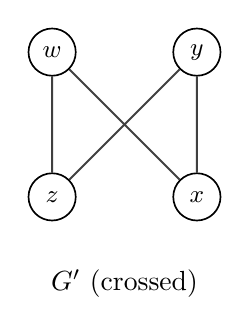
\begin{tikzpicture}[scale=1.3]
  \node[gvlab] (w) at (135:1) {$w$};
  \node[gvlab] (y) at (45:1) {$y$};
  \node[gvlab] (x) at (-45:1) {$x$};
  \node[gvlab] (z) at (-135:1) {$z$};
  \begin{scope}[on background layer]
    \draw[gedge] (w)--(x) (x)--(y) (y)--(z) (z)--(w);
  \end{scope}
  \node at (0,-1.55) {$\Gr'$ (crossed)};
\end{tikzpicture}
\end{center}
Check each edge of $\Gr$ maps to an edge of $\Gr'$: $12\mapsto wx$, $23\mapsto xy$, $34\mapsto yz$,
$41\mapsto zw$ -- all present. As $\varphi$ is a bijection and both graphs have exactly four edges,
the correspondence is onto the edge set as well, so adjacency is preserved in both directions.
\whichrule{Isomorphism is proved by \emph{building} the bijection and verifying $uv$ is an edge iff
$\varphi(u)\varphi(v)$ is; the misleading crossing in the drawing is irrelevant, since position and
edge-crossings are not part of the graph.}
\emph{Check.} Both graphs have degree sequence $(2,2,2,2)$ and four edges, the necessary invariants;
and the explicit $\varphi$ matches all four edges, which is sufficient.
\end{wex}

\begin{wex}{Same degree sequence, different graphs}\label{wex:degseq@c2}
Exhibit two graphs on six vertices that share the degree sequence $(2,2,2,2,2,2)$ but are
\emph{not} isomorphic.
\wrec The trigger is the warning after Definition~\ref{def:iso@c2}: equal degree sequences are
\emph{necessary} but not \emph{sufficient} for isomorphism. To refute sufficiency we need two graphs
with identical degrees that differ in some other invariant.
\wsol Every vertex of degree $2$ forces each graph to be a disjoint union of cycles. Two ways to use
six degree-$2$ vertices: one $6$-cycle $C_6$, or two disjoint triangles $C_3\sqcup C_3$.
\begin{center}
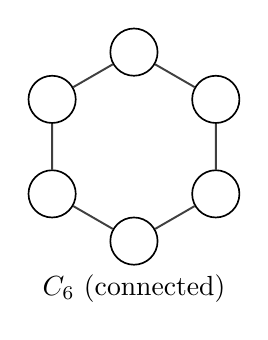
\begin{tikzpicture}[scale=1.2]
  \foreach \i in {0,...,5} { \node[gvlab] (a\i) at ({90-60*\i}:1) {}; }
  \begin{scope}[on background layer]
    \foreach \i [evaluate=\i as \j using {int(mod(\i+1,6))}] in {0,...,5} {
      \draw[gedge] (a\i)--(a\j);
    }
  \end{scope}
  \node at (0,-1.5) {$C_6$ (connected)};
\end{tikzpicture}
\qquad\qquad
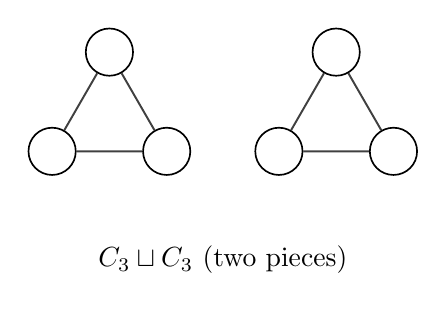
\begin{tikzpicture}[scale=1.2]
  \node[gvlab] (b0) at (90:0.7) {};
  \node[gvlab] (b1) at (210:0.7) {};
  \node[gvlab] (b2) at (330:0.7) {};
  \begin{scope}[on background layer]\draw[gedge] (b0)--(b1) (b1)--(b2) (b2)--(b0);\end{scope}
  \begin{scope}[xshift=2.4cm]
    \node[gvlab] (c0) at (90:0.7) {};
    \node[gvlab] (c1) at (210:0.7) {};
    \node[gvlab] (c2) at (330:0.7) {};
    \begin{scope}[on background layer]\draw[gedge] (c0)--(c1) (c1)--(c2) (c2)--(c0);\end{scope}
  \end{scope}
  \node at (1.2,-1.5) {$C_3\sqcup C_3$ (two pieces)};
\end{tikzpicture}
\end{center}
Both have all degrees $2$ and (by the handshake lemma) $\card{\Eset}=\tfrac{12}{2}=6$ edges, yet
$C_6$ is connected -- a single closed loop -- while $C_3\sqcup C_3$ splits into two components. An
isomorphism preserves connectedness, so no bijection can match them.
\whichrule{To break ``equal degrees $\Rightarrow$ isomorphic'' we exhibit a counterexample
distinguished by a \emph{different} invariant -- here the number of connected components ($1$ versus
$2$) -- which the degree sequence cannot see.}
\emph{Check.} Degree sequences agree: $(2,2,2,2,2,2)$ for each; edge counts agree: $6$ each. They
differ in component count, which suffices to deny isomorphism.
\end{wex}

\begin{method}{How to compute degrees and apply the handshake lemma}
\begin{enumerate}[leftmargin=2em,topsep=2pt,itemsep=1pt]
  \item \textbf{Count locally.} For an undirected graph, $\deg(v)$ is the number of edges incident
  with $v$ (equivalently, $\card{N(v)}$). In a drawing, count the line-ends meeting the dot; never
  count a far endpoint twice.
  \item \textbf{Split direction for digraphs.} Track $d^{+}(v)$ (arrows out) and $d^{-}(v)$ (arrows
  in) separately. They need not be equal at a vertex.
  \item \textbf{Sum and halve.} If you know all degrees, the edge count is
  $\card{\Eset}=\tfrac12\sum_v\deg(v)$ (undirected) or $\card{\Eset}=\sum_v d^{+}(v)=\sum_v d^{-}(v)$
  (directed). If you know $\card{\Eset}$, the degree sum is $2\card{\Eset}$ -- a built-in check on
  any degree count.
  \item \textbf{Use parity.} A claimed degree sequence with an odd number of odd entries is
  impossible (Corollary~\ref{cor:parity@c2}); reject it before drawing.
  \item \textbf{Compare invariants, not pictures.} To decide isomorphism, first compare degree
  sequences (and edge counts, component counts). Matching invariants only suggest isomorphism --
  prove it by exhibiting an adjacency-preserving bijection; a single mismatch disproves it outright.
\end{enumerate}
\end{method}

\begin{pitfall}
A proposed degree sequence must sum to an \emph{even} number, because the sum equals $2\card{\Eset}$.
A sequence like $(3,3,2,2)$ sums to $10$ (even) and may be realizable, but $(3,2,2,2)$ sums to $9$
(odd) and \emph{no} graph has it -- there is no need to attempt a drawing. Equivalently, by
Corollary~\ref{cor:parity@c2}, any list with an odd count of odd numbers is dead on arrival.
\end{pitfall}

\begin{pitfall}
Equal degree sequences do \emph{not} imply isomorphic graphs (Worked
Example~\ref{wex:degseq@c2}), and a misleading drawing does \emph{not} imply non-isomorphic graphs.
The graph is only the incidence pattern: where you place the dots, and whether the edges happen to
cross, carry no information. To settle isomorphism you must either build an explicit
adjacency-preserving bijection (to prove $\cong$) or point to an invariant that differs -- degree
sequence, edge count, number of components, presence of a triangle -- to prove $\not\cong$. Eyeballing
the two pictures is never a proof either way.
\end{pitfall}

\begin{exers}{Exercises.}
\item Let $\Gr$ have vertex set $\set{a,b,c,d,e,f}$ and edge set
$\set{ab,ac,bc,bd,de,df,ef}$. Draw the diagram, list $\deg(v)$ for every vertex, write the degree
sequence, and verify the handshake lemma by computing both $\sum_v\deg(v)$ and $2\card{\Eset}$.

\item Draw the complete graph $K_4$ and the complete graph $K_6$. For each, give the degree of every
vertex and the number of edges, then check your edge counts against the formula $\binom{n}{2}$.

\item Decide, with a one-line reason in each case, which of the following are degree sequences of some
simple graph: $(4,3,2,2,1)$, \ $(3,3,2,1)$, \ $(5,3,2,2,2)$, \ $(2,2,2,2)$. For every realizable one,
draw a graph that achieves it.

\item Draw the digraph on $\set{1,2,3,4}$ with arcs $1\to2,\ 2\to3,\ 3\to1,\ 1\to4,\ 4\to3,\ 3\to3$.
Tabulate $d^{+}(v)$ and $d^{-}(v)$ for each vertex, and verify
$\sum_v d^{+}(v)=\sum_v d^{-}(v)=\card{\Eset}$. (Mind the self-arc $3\to3$.)

\item Prove the handshake lemma directly by induction on the number of edges $\card{\Eset}$, deleting
one edge at the inductive step. State carefully what removing an edge does to the two endpoints'
degrees.

\item A party has $n$ people, some pairs of whom shake hands. Model this as a graph and use
Corollary~\ref{cor:parity@c2} to prove that the number of people who shook hands an odd number of times
is even. Then explain why a group of three people cannot each have shaken hands with exactly one
other person in the group.

\item Let $\Gr$ be the graph on $\set{1,2,3,4,5}$ with edges $\set{12,23,34,45,51,13}$. For
$X=\set{1,2,3,4}$, draw the induced subgraph $\Gr[X]$ and give its degree sequence. Then draw one
spanning subgraph of $\Gr$ that is \emph{not} induced, and one subgraph on $X$ that has strictly fewer
edges than $\Gr[X]$.

\item Show that the two graphs below are isomorphic by giving an explicit vertex bijection and
checking every edge: $\Gr$ has vertices $\set{1,2,3,4,5}$ and edges $\set{12,23,34,45,51}$;
$\Gr'$ has vertices $\set{a,b,c,d,e}$ and edges $\set{ac,ce,eb,bd,da}$. (Both are five-cycles, labelled
differently.)

\item Exhibit two non-isomorphic simple graphs that both have degree sequence $(3,2,2,2,1)$, and name
the invariant that distinguishes them. (Hint: consider whether a triangle is present.)

\item Prove that in any simple graph with at least two vertices there exist two distinct vertices of
equal degree. (Hint: in a graph on $n$ vertices each degree lies in $\set{0,1,\dots,n-1}$; argue that
the values $0$ and $n-1$ cannot both occur, then use pigeonhole.)

\item \emph{Find the bug.} A student claims the sequence $(5,4,3,2,1)$ is realized by some simple
graph on five vertices and starts drawing. Without drawing, show the claim is impossible, and identify
\emph{two} separate reasons (one a counting/parity fact, one about the largest degree relative to the
number of vertices).

\item \emph{Find the bug.} Someone asserts that two graphs are isomorphic ``because both pictures
look like a square with one diagonal, and both have $5$ edges.'' Construct two graphs on four vertices
that each have $5$ edges but are \emph{not} isomorphic -- or explain why no such pair exists on four
vertices -- and state precisely why ``same number of edges'' alone never establishes isomorphism.

\item Prove that for every digraph, the vertices with $d^{+}(v)>d^{-}(v)$ contribute a
total excess exactly balanced by the deficit at vertices with $d^{+}(v)<d^{-}(v)$; that is,
$\sum_v\bigl(d^{+}(v)-d^{-}(v)\bigr)=0$. Explain how this follows from
Proposition~\ref{prop:dirhandshake@c2}.
\end{exers}


\section{Paths, Cycles, Connectivity, and Components}
% ===== Section 2.2: Paths, Cycles, Connectivity, and Components =====
Section~2.1 gave us the static anatomy of a graph -- vertices, edges, and degrees. This
section makes graphs \emph{move}: we follow sequences of edges and ask which vertices can
reach which. The one organizing idea is \emph{reachability} -- ``can I get from $u$ to $v$ by
walking along edges?'' -- and almost everything here is a refinement of it: a walk is any
such trip, a path is a trip that never repeats a vertex, connectivity says every pair is
reachable, and a component is a maximal reachable chunk. These notions are not graph-theoretic
trivia; reachability in a directed graph is exactly how a finite automaton decides whether a
string drives it from the start state into an accept state, and the shortest-walk machinery
below is the breadth-first search that later powers algorithms throughout the book.

\subsection*{Walks, trails, paths, and cycles}

\begin{definition}[Walk, trail, path]\label{def:walk@c2}
Let $\Gr=(\Vset,\Eset)$ be a graph. A \emph{walk} of length $k$ from $u$ to $v$ is an
alternating sequence
\[
  u=v_0,\ e_1,\ v_1,\ e_2,\ v_2,\ \dots,\ e_k,\ v_k=v,
\]
where each $e_i=\set{v_{i-1},v_i}$ is an edge of $\Gr$; its \emph{length} is the number $k$ of
edges traversed (vertices and edges may repeat). A \emph{trail} is a walk with no repeated
\emph{edge}. A \emph{path} is a walk with no repeated \emph{vertex} (hence no repeated edge
either). A walk is \emph{closed} if $v_0=v_k$.
\end{definition}

We usually abbreviate a walk by its vertex list $v_0 v_1\cdots v_k$, since on a simple graph
the intervening edges are forced. The three notions tighten in sequence: every path is a trail,
and every trail is a walk, but not conversely. The distinction matters because the constraints
buy different things -- ``no repeated edge'' (trail) is what Euler tours need, while ``no
repeated vertex'' (path) is what makes a route genuinely simple and bounds its length by
$\card{\Vset}-1$.

\begin{definition}[Cycle]\label{def:cycle@c2}
A \emph{cycle} of length $k\ge 3$ is a closed walk $v_0 v_1\cdots v_{k-1} v_0$ in which
$v_0,\dots,v_{k-1}$ are distinct (so it is a closed path apart from the forced return to the
start). A graph with no cycles is called \emph{acyclic}.
\end{definition}

The lower bound $k\ge 3$ is deliberate for simple graphs: there are no loops (a length-$1$
``cycle'') and no repeated edges (a length-$2$ back-and-forth $v_0 v_1 v_0$ reuses the edge
$\set{v_0,v_1}$), so the shortest genuine cycle is a triangle. The first basic fact is that
walks can always be pruned down to paths -- the workhorse lemma behind everything that follows.

\begin{lemma}[Walks contain paths]\label{lem:walkpath@c2}
If there is a walk from $u$ to $v$ in $\Gr$, then there is a path from $u$ to $v$ in $\Gr$.
\end{lemma}
\begin{proof}
Among all walks from $u$ to $v$, choose one of \emph{minimum length}, say
$W=v_0 v_1\cdots v_k$ with $v_0=u$ and $v_k=v$. We claim $W$ is a path. If not, some vertex
repeats: $v_i=v_j$ with $i<j$. Deleting the segment strictly between the two visits gives the
shorter walk $v_0\cdots v_i v_{j+1}\cdots v_k$ from $u$ to $v$ (it is a walk because $v_i=v_j$,
so $v_i$ and $v_{j+1}$ are adjacent), contradicting minimality. Hence no vertex repeats and $W$
is a path.
\end{proof}

\begin{wex}{Classifying a route as walk, trail, or path}
In the graph below, classify each route from $a$ to $e$:
$R_1=a\,b\,c\,b\,e$,\quad $R_2=a\,b\,d\,c\,b\,e$,\quad $R_3=a\,b\,c\,d\,e$.
\wrec Definition~\ref{def:walk@c2} is a checklist: ``repeats a vertex?'' separates path from
non-path; ``repeats an edge?'' separates trail from non-trail. Read each route off the diagram.
\wsol Here is the graph; every listed step must be a real edge.
\begin{center}
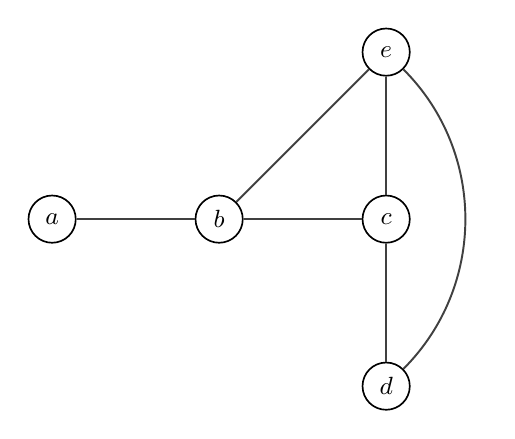
\begin{tikzpicture}[node distance=15mm]
  \node[gvlab] (a) {$a$};
  \node[gvlab,right=of a] (b) {$b$};
  \node[gvlab,right=of b] (c) {$c$};
  \node[gvlab,below=of c] (d) {$d$};
  \node[gvlab,above=of c] (e) {$e$};
  \draw[gedge] (a)--(b);
  \draw[gedge] (b)--(c);
  \draw[gedge] (b)--(e);
  \draw[gedge] (c)--(d);
  \draw[gedge] (c)--(e);
  \draw[gedge] (d) to[bend right=45] (e);
\end{tikzpicture}
\end{center}
$R_1=a\,b\,c\,b\,e$ uses edges $ab,bc,cb,be$. The vertex $b$ repeats, so it is \emph{not} a path;
the edge $\set{b,c}$ is used twice (as $bc$ then $cb$), so it is \emph{not even a trail}. It is a
plain walk of length $4$. $R_3=a\,b\,c\,d\,e$ uses $ab,bc,cd,de$, all distinct edges and all five
vertices distinct -- a \emph{path} of length $4$. (The middle route $R_2$ was a deliberate
trap: $\set{a,b},\set{b,d}$ is not an edge list of this graph, since $b$ and $d$ are not
adjacent, so $R_2$ is not a route at all.)
\whichrule{The vertex-repetition test is the sharper one: a repeated vertex already disqualifies
``path,'' and you only fall back to the edge-repetition test to decide between ``trail'' and
``mere walk.''}
\emph{Check.} $R_1$ has length $4$ on $5$ symbols $a,b,c,b,e$ -- the duplicate $b$ is visible in
the list, confirming it is not a path. $R_3$ visits each of $a,b,c,d,e$ once.
\end{wex}

\subsection*{Connectivity and components}

\begin{definition}[Connected, component]\label{def:conn@c2}
Define a relation on $\Vset$ by $u\sim v$ iff there is a walk (equivalently, by
Lemma~\ref{lem:walkpath@c2}, a path) from $u$ to $v$. This $\sim$ is an equivalence relation; its
equivalence classes are the \emph{connected components} of $\Gr$. A graph is \emph{connected} if
it has exactly one component, i.e.\ every pair of vertices is joined by a path.
\end{definition}

That $\sim$ is an equivalence relation is the quiet engine of the whole subject, so we verify
it. \emph{Reflexive}: the length-$0$ walk $v$ joins $v$ to itself. \emph{Symmetric}: reversing a
walk from $u$ to $v$ gives one from $v$ to $u$. \emph{Transitive}: concatenating a $u$-to-$v$
walk with a $v$-to-$w$ walk yields a $u$-to-$w$ walk. Because the classes of an equivalence
relation \emph{partition} the vertex set, every vertex lies in exactly one component, and there
is never any edge between two different components -- if there were, its endpoints would be
joined and hence in the same class.

\begin{wex}{Counting components}
How many connected components does the following graph have, and what are they?
\wrec ``Component'' = one $\sim$-class = one maximal reachable island. Trace reachability
outward from an unvisited vertex until it stops, mark that island, then start fresh from any
still-unvisited vertex.
\wsol
\begin{center}
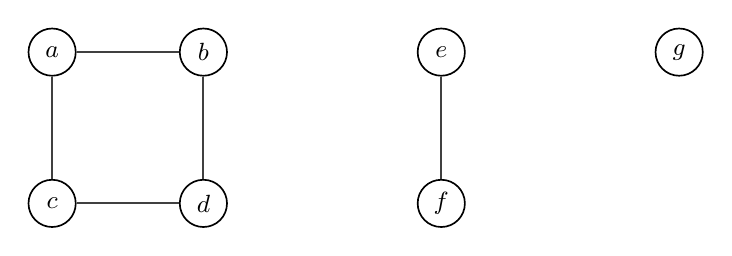
\begin{tikzpicture}[node distance=13mm]
  \node[gvlab] (a) {$a$};
  \node[gvlab,right=of a] (b) {$b$};
  \node[gvlab,below=of a] (c) {$c$};
  \node[gvlab,below=of b] (d) {$d$};
  \node[gvlab,right=2.4cm of b] (e) {$e$};
  \node[gvlab,below=of e] (f) {$f$};
  \node[gvlab,right=2.4cm of e] (g) {$g$};
  \draw[gedge] (a)--(b);
  \draw[gedge] (a)--(c);
  \draw[gedge] (b)--(d);
  \draw[gedge] (c)--(d);
  \draw[gedge] (e)--(f);
\end{tikzpicture}
\end{center}
Start at $a$: reachable set grows $\set{a}\to\set{a,b,c}\to\set{a,b,c,d}$ and then stops, since no edge
leaves $\set{a,b,c,d}$. That is the first component. Now pick the unvisited $e$: reachability
gives $\set{e,f}$ and stops. Finally $g$ has no incident edge, so it is an \emph{isolated vertex}
and a component by itself. Three components: $\set{a,b,c,d}$, $\set{e,f}$, and $\set{g}$.
\whichrule{Components are the $\sim$-classes, and $\sim$ is found by flood-fill: expand the
reachable frontier from a seed until it closes off, which is precisely one maximal connected
piece.}
\emph{Check.} The three classes are disjoint and cover all seven vertices ($4+2+1=7$), and no
drawn edge crosses between them -- both hallmarks of a partition into components.
\end{wex}

The proposition below records how connectivity constrains the edge count; it is the bridge to trees
in Section~2.3 and the reason ``$n-1$ edges'' will keep reappearing.

\begin{proposition}[A connected graph has at least $n-1$ edges]\label{prop:nminus1@c2}
If $\Gr$ is connected with $n=\card{\Vset}$ vertices, then $\card{\Eset}\ge n-1$.
\end{proposition}
\begin{proof}
Build $\Gr$ by adding its edges one at a time, starting from the edgeless graph on $\Vset$,
which has $n$ components (one per vertex). Adding a single edge $\set{x,y}$ can lower the
component count by \emph{at most one}: it merges the component of $x$ with the component of $y$
if they differ, and changes nothing if they already coincide. To reach a connected graph
($1$ component) from $n$ components, we must drop the count by $n-1$, and since each edge drops
it by at most $1$, at least $n-1$ edges are required.
\end{proof}

\begin{method}{Finding the components of a graph}
\begin{enumerate}[leftmargin=1.6em,topsep=2pt,itemsep=1pt]
\item Mark every vertex ``unvisited'' and set a component counter to $0$.
\item While some vertex is unvisited, pick one as a \emph{seed}, increment the counter, and run
a search (below) from it; everything the search reaches is one component.
\item \textbf{The search.} Keep a frontier, initially just the seed. Repeatedly take a frontier
vertex, mark it visited, and add its still-unvisited neighbours to the frontier. Stop when the
frontier empties.
\item When all vertices are visited, the counter is the number of components, and the visited
sets recorded per seed are the components themselves.
\end{enumerate}
\end{method}

\subsection*{Distance and breadth-first search}

If a path exists, we usually want the \emph{shortest} one. Counting edges along shortest paths
turns a graph into a metric space and is the first place graph search becomes quantitative.

\begin{definition}[Distance]\label{def:dist@c2}
The \emph{distance} $d(u,v)$ between vertices $u,v$ is the length of a shortest $u$--$v$ walk,
or $\infty$ if no walk exists (i.e.\ $u\not\sim v$). By Lemma~\ref{lem:walkpath@c2} a shortest walk
is a path, so $d(u,v)$ equals the length of a shortest \emph{path}.
\end{definition}

\emph{Breadth-first search} (BFS) computes $d(s,\cdot)$ from a fixed source $s$ by exploring the
graph in concentric ``layers'': layer $0$ is $\set{s}$; layer $i+1$ is every not-yet-seen vertex
adjacent to a layer-$i$ vertex. A vertex's layer index is exactly its distance from $s$. The
following example runs it.

\begin{wex}{Breadth-first search and distances from a source}
Run BFS from $s$ on the graph below and read off $d(s,v)$ for every vertex.
\wrec ``Shortest path from one source'' is the BFS trigger: peel the graph into distance layers
$L_0,L_1,L_2,\dots$, never revisiting a vertex, and the layer a vertex lands in is its distance.
\wsol
\begin{center}
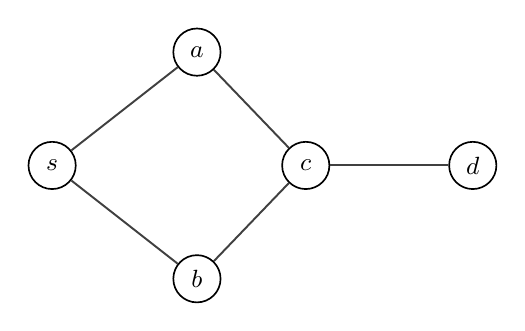
\begin{tikzpicture}[node distance=15mm]
  \node[gvlab] (s) {$s$};
  \node[gvlab,above right=10mm and 14mm of s] (a) {$a$};
  \node[gvlab,below right=10mm and 14mm of s] (b) {$b$};
  \node[gvlab,right=2.6cm of s] (c) {$c$};
  \node[gvlab,right=of c] (d) {$d$};
  \draw[gedge] (s)--(a);
  \draw[gedge] (s)--(b);
  \draw[gedge] (a)--(c);
  \draw[gedge] (b)--(c);
  \draw[gedge] (c)--(d);
\end{tikzpicture}
\end{center}
$L_0=\set{s}$. Neighbours of $s$ not yet seen: $a,b$, so $L_1=\set{a,b}$. New neighbours of
$L_1$: from $a$ we reach $c$, from $b$ we also reach $c$ (recorded once), so $L_2=\set{c}$. New
neighbours of $L_2$: from $c$ we reach $d$, so $L_3=\set{d}$. The frontier is now empty. Reading
layers off as distances:
\[
  d(s,s)=0,\quad d(s,a)=d(s,b)=1,\quad d(s,c)=2,\quad d(s,d)=3.
\]
\whichrule{BFS visits vertices in nondecreasing distance order, so the first time a vertex is
seen is along a shortest path; its layer index is therefore its exact distance from $s$.}
\emph{Check.} A shortest $s$--$d$ path is $s\,a\,c\,d$ (length $3$), matching $d(s,d)=3$; there
is no shorter route because $d$'s only neighbour $c$ already sits at distance $2$.
\end{wex}

A useful structural fact, also from BFS layering, is that a shortest path never skips a layer:
consecutive vertices on it differ in distance by exactly one. We state the cleaner triangle
form, which is all later chapters need.

\begin{proposition}[Triangle inequality for graph distance]\label{prop:triangle@c2}
For all vertices $u,v,w$ in the same component, $d(u,w)\le d(u,v)+d(v,w)$.
\end{proposition}
\begin{proof}
Take a shortest $u$--$v$ path $P$ (length $d(u,v)$) and a shortest $v$--$w$ path $Q$ (length
$d(v,w)$). Concatenating $P$ then $Q$ is a $u$--$w$ \emph{walk} of length $d(u,v)+d(v,w)$. By
Lemma~\ref{lem:walkpath@c2} it contains a $u$--$w$ path, whose length is at most the walk's length,
and $d(u,w)$ is the minimum over all such paths, so $d(u,w)\le d(u,v)+d(v,w)$.
\end{proof}

\subsection*{Euler and Hamilton: traversing edges versus visiting vertices}

Two of the oldest questions in graph theory ask for a route that hits everything exactly once --
but ``everything'' can mean the \emph{edges} or the \emph{vertices}, and the two problems could
not differ more in difficulty. They preview a theme that drives the whole book: superficially
similar problems can sit on opposite sides of the tractable/intractable line.

\begin{definition}[Eulerian and Hamiltonian]\label{def:eulham@c2}
An \emph{Euler trail} is a trail using every edge of $\Gr$ exactly once; an \emph{Euler circuit}
is a closed such trail. A \emph{Hamilton path} is a path visiting every vertex exactly once; a
\emph{Hamilton cycle} is a cycle doing so.
\end{definition}

The Euler side has a clean, checkable criterion -- Euler's theorem: a connected graph has an
Euler circuit iff every vertex has \emph{even} degree, and an Euler trail (open) iff exactly two
vertices have odd degree. The reason is a local parity count: each time a circuit passes through
a vertex it uses two incident edges (one in, one out), so traversing all edges forces every
degree to be even. The Hamilton side has \emph{no} such efficient test known; deciding whether a
graph has a Hamilton path is (in its directed $s$-to-$t$ form) the problem $\HAMPATH$, which is
$\classNP$-complete (Chapter~13). Keep the contrast in view: counting degrees is easy, but routing
through all vertices is, as far as anyone knows, hard.

\begin{wex}{Euler circuit by the even-degree test}
Does the graph below have an Euler circuit, an open Euler trail, or neither? If a circuit
exists, exhibit one.
\wrec The Euler criterion is purely a degree-parity check: count odd-degree vertices. Zero of
them means a closed Euler circuit; exactly two means an open Euler trail; anything else means
neither.
\wsol
\begin{center}
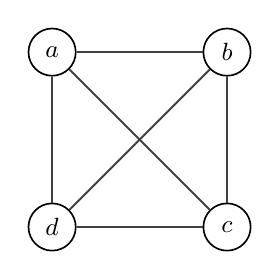
\begin{tikzpicture}[node distance=16mm]
  \node[gvlab] (a) {$a$};
  \node[gvlab,right=of a] (b) {$b$};
  \node[gvlab,below=of b] (c) {$c$};
  \node[gvlab,below=of a] (d) {$d$};
  \draw[gedge] (a)--(b);
  \draw[gedge] (b)--(c);
  \draw[gedge] (c)--(d);
  \draw[gedge] (d)--(a);
  \draw[gedge] (a)--(c);
  \draw[gedge] (b)--(d);
\end{tikzpicture}
\end{center}
This is $K_4$. Each vertex is joined to the other three, so $\deg(a)=\deg(b)=\deg(c)=\deg(d)=3$,
which is \emph{odd}. With four odd-degree vertices (not zero and not two), the criterion says
\emph{neither} an Euler circuit nor an open Euler trail exists. No traversal can use all six
edges without repeating one.
\whichrule{Euler's theorem reduces the global routing question to a local parity count; here
four odd degrees instantly rule out any edge-exact traversal, so we need not search at all.}
\emph{Check.} Sum of degrees $=4\cdot 3=12=2\card{\Eset}$, giving $\card{\Eset}=6$, the six
edges of $K_4$ -- and a graph with more than two odd-degree vertices can never be traced in one
edge-disjoint sweep.
\end{wex}

\begin{wex}{An Euler trail that is not a circuit; and a Hamilton cycle}
For the graph below, (i) find an open Euler trail, and (ii) find a Hamilton cycle.
\wrec Part (i) is again the parity test -- look for exactly two odd-degree vertices and start the
trail at one of them. Part (ii) is the vertex-visiting question, with no shortcut criterion: we
must exhibit a cycle through all vertices by hand.
\wsol
\begin{center}
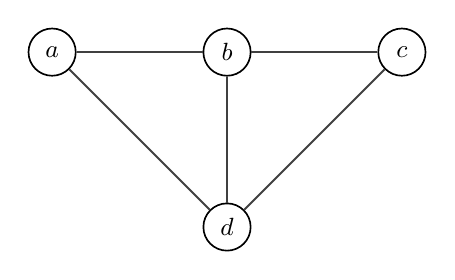
\begin{tikzpicture}[node distance=16mm]
  \node[gvlab] (a) {$a$};
  \node[gvlab,right=of a] (b) {$b$};
  \node[gvlab,right=of b] (c) {$c$};
  \node[gvlab,below=of b] (d) {$d$};
  \draw[gedge] (a)--(b);
  \draw[gedge] (b)--(c);
  \draw[gedge] (a)--(d);
  \draw[gedge] (d)--(c);
  \draw[gedge] (b)--(d);
\end{tikzpicture}
\end{center}
\emph{(i) Euler trail.} Degrees: $\deg(a)=2$ ($ab,ad$), $\deg(c)=2$ ($cb,cd$), $\deg(b)=3$
($ba,bc,bd$), $\deg(d)=3$ ($da,dc,db$). Exactly two odd-degree vertices, $b$ and $d$, so an open
Euler trail exists and must start at one of them. Starting at $b$:
$b\,a\,d\,c\,b\,d$ uses $ba,ad,dc,cb,bd$ -- all five edges exactly once, ending at $d$. That is an
Euler trail.
\emph{(ii) Hamilton cycle.} We need a cycle through all four vertices. Try $a\,b\,c\,d\,a$: the
required edges are $ab,bc,cd,da$, and all four are present, returning to $a$. So $a\,b\,c\,d\,a$
is a Hamilton cycle.
\whichrule{The two odd-degree vertices pin down where an Euler trail can begin and end; the
Hamilton cycle, having no degree criterion, is produced by exhibiting one concrete vertex
ordering whose consecutive pairs are all edges.}
\emph{Check.} The Euler trail $b\,a\,d\,c\,b\,d$ lists $6$ vertices hence $5$ edges, matching
$\card{\Eset}=5$; the Hamilton cycle $a\,b\,c\,d\,a$ visits each of the four vertices once before
closing.
\end{wex}

\begin{wex}{Reachability in a digraph: when direction breaks symmetry}
In the directed graph below, decide for each pair of vertices $u,v$ whether $u$ can reach $v$
and vice versa, and explain why connectivity in digraphs is subtler than in graphs.
\wrec Directed reachability follows arrows \emph{one way}, so the relation ``$u$ reaches $v$'' is
no longer symmetric. Test reachability separately in each direction by tracing forward along
arrowheads only.
\wsol
\begin{center}
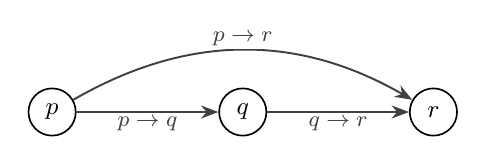
\begin{tikzpicture}[>={Stealth[length=2.2mm]},node distance=18mm]
  \node[gvlab] (p) {$p$};
  \node[gvlab,right=of p] (q) {$q$};
  \node[gvlab,right=of q] (r) {$r$};
  \draw[gedge,->] (p)-- node[gvlbl,below]{$p\to q$} (q);
  \draw[gedge,->] (q)-- node[gvlbl,below]{$q\to r$} (r);
  \draw[gedge,->] (p) to[bend left=30] node[gvlbl,above]{$p\to r$} (r);
\end{tikzpicture}
\end{center}
Following arrows: from $p$ we reach $q$ (edge $p\to q$), $r$ (edge $p\to r$, or via $q$). From
$q$ we reach $r$. But from $r$ there are \emph{no} outgoing edges, so $r$ reaches nothing; and
$q$ cannot reach $p$, since both arrows at $p$ point away from it. Thus $p$ reaches everyone,
yet no one reaches $p$. The underlying \emph{undirected} graph (forget arrowheads) is connected,
but directed reachability is one-way, so $\sim$ from Definition~\ref{def:conn@c2} is not symmetric
here. This is why digraphs distinguish \emph{strong} connectivity (every $u$ reaches every $v$
by a directed path) from \emph{weak} connectivity (the underlying graph is connected).
\whichrule{Dropping symmetry is exactly the feature that makes a digraph model a computation:
a finite automaton is a digraph whose directed reachability from the start state to an accept
state decides membership, and you cannot run those transitions backward.}
\emph{Check.} The pair $(p,r)$ is reachable in the order $p\rightsquigarrow r$ but not
$r\rightsquigarrow p$, so the relation genuinely fails symmetry; the underlying undirected
$p$--$q$--$r$ with the chord $pr$ is nonetheless one connected piece.
\end{wex}

\begin{pitfall}
\textbf{Path versus walk versus trail.} The three are routinely conflated. A \emph{walk} permits
any repetition; a \emph{trail} forbids repeating an \emph{edge}; a \emph{path} forbids repeating
a \emph{vertex}. When a result says ``there is a path,'' you may assume distinct vertices and
length at most $n-1$; when it says only ``there is a walk,'' you may not -- prune it with
Lemma~\ref{lem:walkpath@c2} first.
\end{pitfall}

\begin{pitfall}
\textbf{An isolated vertex is its own component.} Counting components, do not overlook
degree-$0$ vertices: each is a singleton $\sim$-class. A graph drawn as one ``main blob'' plus a
few stray dots has more than one component, and ``connected'' fails the moment a single vertex is
unreachable from the rest.
\end{pitfall}

\begin{pitfall}
\textbf{Even degree is the Euler test, not the Hamilton test.} The clean degree-parity criterion
governs \emph{Euler} routes (every edge once). It says \emph{nothing} about \emph{Hamilton}
routes (every vertex once): graphs with all-even degrees can lack a Hamilton cycle, and graphs
with odd degrees can have one. There is no known efficient degree criterion for the Hamilton
problem -- that is the gist of its $\classNP$-completeness.
\end{pitfall}

\begin{exers}{Exercises.}
\item Consider the graph on vertices $\set{a,b,c,d,e}$ with edges
$\set{a,b},\set{b,c},\set{c,d},\set{d,e},\set{e,a},\set{a,c}$. Draw it, then for the route
$a\,b\,c\,a\,c\,d$ decide whether it is a walk, a trail, or a path, and give its length. Find a
genuine path from $b$ to $d$ and a closed walk that is not a cycle.

\item Prove that in any graph, if there is a trail from $u$ to $v$ then there is a path from $u$
to $v$. (You may cite Lemma~\ref{lem:walkpath@c2}, but state precisely which hypothesis you use.)

\item Draw a connected graph on $6$ vertices with exactly $5$ edges, and a disconnected graph on
$6$ vertices with exactly $5$ edges. What does Proposition~\ref{prop:nminus1@c2} say must be true of
the first, and why does it not contradict the existence of the second?

\item For the graph with vertices $\set{1,2,3,4,5,6,7}$ and edges
$\set{1,2},\set{2,3},\set{1,3},\set{4,5},\set{6,7},\set{5,6}$, list the connected components and
state how many there are. Identify any isolated vertices.

\item Run breadth-first search from vertex $s$ on a graph of your own drawing in which some
vertex lies at distance exactly $3$ from $s$. Label each vertex with its distance $d(s,\cdot)$,
and exhibit one shortest path realizing the distance $3$.

\item Prove that a graph $\Gr$ with at least one vertex is connected if and only if for every
partition of $\Vset$ into two nonempty sets $X$ and $Y$, at least one edge has one endpoint in $X$
and the other in $Y$.

\item Determine, using only a degree count, whether each graph has an Euler circuit, an open
Euler trail, or neither: (a) the cycle $C_5$; (b) the complete bipartite graph $K_{2,3}$;
(c) the complete graph $K_5$. State the degree of a typical vertex in each.

\item Design a connected graph on exactly $6$ vertices that has an open Euler trail but no Euler
circuit, and has a Hamilton cycle. Draw it, mark the two odd-degree vertices, and write out both
the Euler trail and the Hamilton cycle as vertex sequences.

\item Prove the contrapositive of one direction of Euler's criterion: if a connected graph has a
vertex of odd degree, then it has no Euler circuit. (Hint: count how many edges incident to that
vertex a closed trail must use, and argue by parity.)

\item In the directed graph on $\set{p,q,r,s}$ with arcs $p\to q$, $q\to r$, $r\to s$, $s\to q$,
decide which vertices can reach which. Is the digraph strongly connected? Is its underlying
undirected graph connected? Explain the difference in one sentence.

\item \emph{Find the bug.} A student claims that ``every connected graph on $n$ vertices with
exactly $n-1$ edges contains a cycle.'' Draw a small counterexample, and state the correct
relationship between ``$n-1$ edges'' and ``acyclic'' that they should have written instead.

\item \emph{Find the bug.} Someone asserts: ``A graph has a Hamilton cycle if and only if every
vertex has degree at least $2$.'' Give a graph in which every vertex has degree at least $2$ yet
no Hamilton cycle exists, and explain in one sentence why no simple degree condition can settle
the Hamilton question.
\end{exers}


\section{Trees and Spanning Trees}
A \emph{tree} is the leanest possible connected graph: connected, but with not one edge to
spare. This single tension -- enough edges to hold the vertices together, but so few that
removing any one disconnects the graph -- forces a remarkable rigidity, and the one key idea of
this section is that several superficially different descriptions of that rigidity all pick out
exactly the same graphs. We prove the equivalence, count the edges of a tree, locate its leaves,
add a root to turn an undirected tree into the branching structure used for parse and computation
trees later in the book, and finish with spanning trees -- the tree skeletons hiding inside every
connected graph.

\begin{definition}[Forest, tree, leaf]\label{def:tree@c2}
A graph is \emph{acyclic} if it contains no cycle. A \emph{forest} is an acyclic graph; a
\emph{tree} is a connected forest, i.e.\ a connected acyclic graph. A vertex of degree $1$ in a
tree is a \emph{leaf}; a vertex of degree $\ge 2$ is an \emph{internal} vertex. The connected
components of a forest are exactly its constituent trees.
\end{definition}

Throughout, $n=\card{V}$ denotes the number of vertices and $m=\card{E}$ the number of edges of
the graph under discussion. The next two lemmas are the workhorses; they are easy on their own and
combine into the characterization theorem.

\begin{lemma}[Every tree on $\ge 2$ vertices has a leaf]\label{lem:leaf@c2}
A tree $T$ with $n\ge 2$ vertices has at least two leaves.
\end{lemma}
\begin{proof}
Take a \emph{longest} path $P=v_0v_1\cdots v_k$ in $T$ (a longest path exists because $T$ is finite
and, with $n\ge 2$ and $T$ connected, has length $k\ge 1$). We claim its endpoint $v_0$ is a leaf.
Suppose not: then $v_0$ has a neighbour $u$ besides $v_1$. If $u$ lies off $P$, then
$u\,v_0v_1\cdots v_k$ is a longer path, contradicting maximality. If instead $u=v_j$ for some
$j\ge 2$, then $v_0v_1\cdots v_j v_0$ is a cycle, contradicting acyclicity. So $v_0$ has only the
neighbour $v_1$ and is a leaf; the same argument at $v_k$ gives a second leaf.
\end{proof}

\begin{lemma}[Edge count]\label{lem:edges@c2}
Every tree with $n$ vertices has exactly $n-1$ edges.
\end{lemma}
\begin{proof}
Induct on $n$. For $n=1$ the only tree is a single vertex with $0=n-1$ edges. For $n\ge 2$, by
Lemma~\ref{lem:leaf@c2} pick a leaf $\ell$. Deleting $\ell$ and its one incident edge yields a graph
$T'$ on $n-1$ vertices: $T'$ is still acyclic (deleting cannot create a cycle), and still connected
(any path in $T$ between two surviving vertices could only have used $\ell$ as an interior vertex,
but $\ell$ has degree $1$ and cannot be interior). So $T'$ is a tree on $n-1$ vertices, with
$(n-1)-1$ edges by induction, and $T$ has one more, namely $n-1$.
\end{proof}

We can now collect the standard descriptions of a tree and prove they coincide. This is the central
result of the section; later we use whichever clause is most convenient.

\begin{theorem}[Equivalent characterizations of a tree]\label{thm:treechar@c2}
Let $G$ be a graph with $n\ge 1$ vertices and $m$ edges. The following are equivalent.
\begin{enumerate}[label=\textup{(\roman*)},leftmargin=2.4em,topsep=2pt,itemsep=1pt]
  \item $G$ is a tree (connected and acyclic).
  \item Every two vertices of $G$ are joined by exactly one path.
  \item $G$ is connected and $m=n-1$.
  \item $G$ is acyclic and $m=n-1$.
  \item $G$ is connected, but deleting any edge disconnects it (\emph{minimally connected}).
  \item $G$ is acyclic, but adding any edge between two non-adjacent vertices creates a cycle
        (\emph{maximally acyclic}).
\end{enumerate}
\end{theorem}
\begin{proof}
We show (i)$\Rightarrow$(ii)$\Rightarrow$(iii)$\Rightarrow$(iv)$\Rightarrow$(i), then
(i)$\Leftrightarrow$(v) and (i)$\Leftrightarrow$(vi).

\emph{(i)$\Rightarrow$(ii).} Connectivity gives at least one path between any $u,v$. If two distinct
$u$--$v$ paths existed, their symmetric difference would contain a cycle, contradicting acyclicity;
so the path is unique.

\emph{(ii)$\Rightarrow$(iii).} Unique paths imply connectivity. For the count, the unique-path
property makes $G$ acyclic (a cycle would give two paths between two of its vertices), so $G$ is a
tree and Lemma~\ref{lem:edges@c2} gives $m=n-1$.

\emph{(iii)$\Rightarrow$(iv).} Suppose $G$ is connected with $m=n-1$ but contains a cycle. Delete one
edge of that cycle; the graph stays connected (the deleted edge's endpoints are still joined by the
rest of the cycle). Repeat until acyclic; the result is a connected acyclic graph, i.e.\ a tree, on
$n$ vertices, which by Lemma~\ref{lem:edges@c2} has $n-1$ edges. But we deleted at least one edge from
the original $n-1$, leaving $\le n-2$, a contradiction. Hence $G$ is acyclic with $m=n-1$.

\emph{(iv)$\Rightarrow$(i).} Let $G$ be acyclic with $m=n-1$, and let its components be
$T_1,\dots,T_c$ with $n_i$ vertices each. Every component is connected and acyclic, hence a tree, so
$T_i$ has $n_i-1$ edges. Summing, $m=\sum_i (n_i-1)=n-c$. With $m=n-1$ we get $c=1$: $G$ is
connected, so it is a tree.

\emph{(i)$\Leftrightarrow$(v).} If $G$ is a tree and $e=uv$ is an edge, then by (ii) $e$ itself is the
\emph{only} $u$--$v$ path; deleting it leaves no $u$--$v$ path, so $G$ disconnects. Conversely, if $G$
is minimally connected it is connected, and acyclic: any edge lying on a cycle could be removed
without disconnecting (its endpoints stay joined through the rest of the cycle), violating minimality.

\emph{(i)$\Leftrightarrow$(vi).} If $G$ is a tree and $u,v$ are non-adjacent, the unique $u$--$v$ path
together with the new edge $uv$ forms a cycle, so $G$ is maximally acyclic. Conversely a maximally
acyclic graph is acyclic; it is connected, for if $u,v$ were in different components the edge $uv$
could be added without creating a cycle (no path between them existed), contradicting maximality.
\end{proof}

\begin{corollary}[Adding or removing one edge]\label{cor:onee@c2}
In a tree, removing any edge produces exactly two components, and adding any edge between
non-adjacent vertices produces exactly one cycle.
\end{corollary}
\begin{proof}
Removing edge $uv$ disconnects $G$ (clause (v)); the two components are the side reachable from $u$
and the side reachable from $v$, and there are exactly two because the remaining graph has
$n$ vertices and $(n-1)-1=n-2$ edges, forcing $c=n-(n-2)=2$ by the count in (iv). Adding a
non-edge creates a cycle (clause (vi)); it is unique because two cycles would share the new edge and
their symmetric difference would contain a cycle already present in the tree.
\end{proof}

It is worth seeing the four most-used clauses of Theorem~\ref{thm:treechar@c2} laid out as a closed
ring, to make plain that no one of them is the ``real'' definition -- each forces the other three.
%% ============================================================
%% FIGURE 2B -- TREE-CHARACTERIZATION EQUIVALENCE.
%%   ID:        FIG 2B (concept-map equivalence ring, class A gap)
%%   Placement: Section 2.3, just after Theorem 2.3.x (thm:treechar) and
%%              Corollary 2.3.x, before the "Recognizing a tree" example.
%%   Purpose:   show the four standard tree characterizations are mutually
%%              equivalent -- any one forces the other three.
%%   Objects:   four cnodes for a graph on n vertices:
%%              (T1) connected and acyclic; (T2) connected and |E|=n-1;
%%              (T3) acyclic and |E|=n-1; (T4) unique simple path between
%%              every two vertices.
%%   Arrows:    bidirectional cbidir arrows around a 4-node ring, so every
%%              pair is linked through the cycle of equivalences.
%%   Invariant: all four conditions pick out the same class -- "tree".
%%   Caption:   takeaway sentence below the figure.
%%   Validation: these are the standard equivalent tree characterizations:
%%              any two of {connected, acyclic, |E|=n-1} imply the third,
%%              and a tree has a unique path between any two vertices.
%% ============================================================
\begin{center}
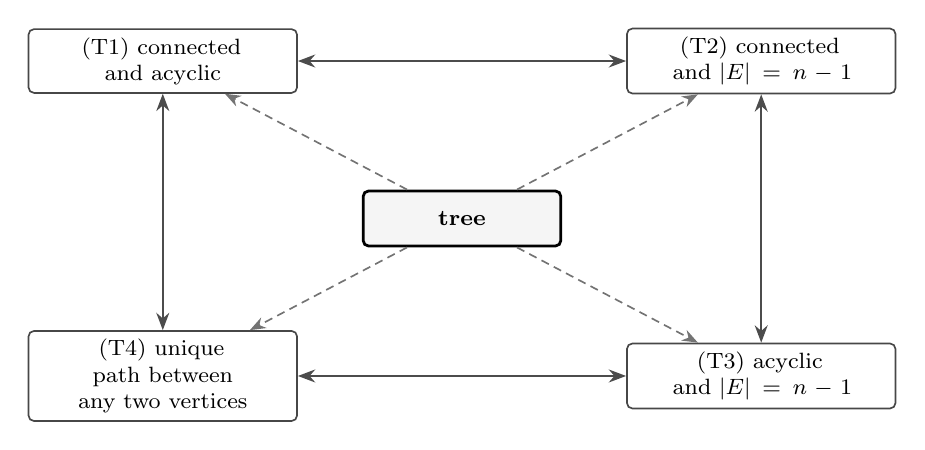
\begin{tikzpicture}[scale=1.0]
  \node[cnodew] (T1) at (-3.8,2.0) {(T1) connected\\and acyclic};
  \node[cnodew] (T2) at (3.8,2.0) {(T2) connected\\and $\card{E}=n-1$};
  \node[cnodew] (T3) at (3.8,-2.0) {(T3) acyclic\\and $\card{E}=n-1$};
  \node[cnodew] (T4) at (-3.8,-2.0) {(T4) unique path between\\any two vertices};
  \draw[cbidir] (T1) -- (T2);
  \draw[cbidir] (T2) -- (T3);
  \draw[cbidir] (T3) -- (T4);
  \draw[cbidir] (T4) -- (T1);
  \node[croot] (hub) at (0,0) {tree};
  \draw[cdash] (hub) -- (T1);
  \draw[cdash] (hub) -- (T2);
  \draw[cdash] (hub) -- (T3);
  \draw[cdash] (hub) -- (T4);
\end{tikzpicture}
\end{center}
Read any double arrow as ``$\Leftrightarrow$'': the ring says the four conditions are interchangeable,
so each one alone defines the same class (the hub ``tree''), and one may verify whichever clause is
cheapest on the graph at hand.
\emph{Check.} On an $n$-vertex graph, any two of $\set{\text{connected},\text{acyclic},\card{E}=n-1}$
force the third (Lemma~\ref{lem:edges@c2} and clauses (iii), (iv) of Theorem~\ref{thm:treechar@c2}), and a
tree has a unique simple path between any two vertices (clause (ii)); hence T1--T4 are equivalent.

\begin{wex}{Recognizing a tree from a drawing}
Of the two graphs below on vertex set $\set{a,b,c,d,e}$, decide which is a tree.
\begin{center}
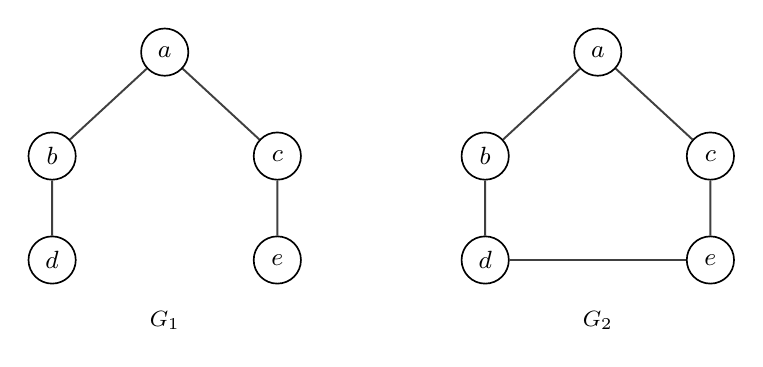
\begin{tikzpicture}[scale=1.1]
  \node[gvlab] (a) at (0,1.2) {$a$};
  \node[gvlab] (b) at (-1.3,0) {$b$};
  \node[gvlab] (c) at (1.3,0) {$c$};
  \node[gvlab] (d) at (-1.3,-1.2) {$d$};
  \node[gvlab] (e) at (1.3,-1.2) {$e$};
  \begin{scope}[on background layer]
    \draw[gedge] (a)--(b); \draw[gedge] (a)--(c);
    \draw[gedge] (b)--(d); \draw[gedge] (c)--(e);
  \end{scope}
  \node[font=\footnotesize] at (0,-1.9) {$G_1$};
  \begin{scope}[xshift=5cm]
    \node[gvlab] (a2) at (0,1.2) {$a$};
    \node[gvlab] (b2) at (-1.3,0) {$b$};
    \node[gvlab] (c2) at (1.3,0) {$c$};
    \node[gvlab] (d2) at (-1.3,-1.2) {$d$};
    \node[gvlab] (e2) at (1.3,-1.2) {$e$};
    \begin{scope}[on background layer]
      \draw[gedge] (a2)--(b2); \draw[gedge] (a2)--(c2);
      \draw[gedge] (b2)--(d2); \draw[gedge] (c2)--(e2);
      \draw[gedge] (d2)--(e2);
    \end{scope}
    \node[font=\footnotesize] at (0,-1.9) {$G_2$};
  \end{scope}
\end{tikzpicture}
\end{center}
\wrec The fastest test pairs the edge count against connectivity (clause (iii)): a tree on $n$
vertices has exactly $n-1$ edges, so any deviation rules a tree out instantly, and the matching
count plus visible connectivity rules one in.
\wsol Here $n=5$, so a tree needs exactly $4$ edges. $G_1$ has $4$ edges and is clearly connected
(every vertex reaches $a$), so $G_1$ is a tree. $G_2$ has $5$ edges; since $5\ne 4$, $G_2$ is not a
tree -- indeed the extra edge $de$ closes the cycle $b\,a\,c\,e\,d\,b$.
\whichrule{Clause (iii) of Theorem~\ref{thm:treechar@c2} turns ``is it a tree?'' into a one-glance
arithmetic check: count edges, compare with $n-1$, then confirm connectivity (or, for the converse,
acyclicity).}
\emph{Check.} In $G_1$, deleting edge $ab$ splits off exactly $\set{b,d}$ from $\set{a,c,e}$ --- two
components, as Corollary~\ref{cor:onee@c2} predicts. In $G_2$, the path from $b$ to $e$ is not unique
($b\,d\,e$ and $b\,a\,c\,e$), confirming via clause (ii) that $G_2$ is not a tree.
\end{wex}

\textbf{Rooted trees.} Designating one vertex as the \emph{root} orients a tree: every other vertex
has a unique path back to the root (clause (ii)), and the first step of that path points at the
vertex's \emph{parent}. This is the form trees take when they record a computation or a derivation.

\begin{definition}[Rooted tree]\label{def:rooted@c2}
A \emph{rooted tree} is a tree $T$ with a distinguished vertex $r$, the \emph{root}. For a vertex
$v\ne r$, the \emph{parent} of $v$ is the neighbour of $v$ on the unique $v$--$r$ path; the other
neighbours of $v$ are its \emph{children}, and every neighbour of $r$ is a child of $r$. A leaf of a
rooted tree is a vertex with no children. The
\emph{depth} of $v$ is the length of the $v$--$r$ path; the \emph{height} of $T$ is the maximum
depth.
\end{definition}

Drawn with the root at top and children below their parent, a rooted tree is the picture we will use
for grammar derivations and the branching runs of nondeterministic machines.

\begin{wex}{Reading parent, depth, and leaves off a rooted tree}
The rooted tree below has root $r$. Identify the children of $x$, the depth of $z$, and all leaves.
\begin{center}
\begin{tikzpicture}[level distance=12mm,
   level 1/.style={sibling distance=30mm},
   level 2/.style={sibling distance=15mm},
   every node/.style={gvlab},
   edge from parent/.style={tedge,draw}]
  \node {$r$}
    child {node (x) {$x$}
      child {node {$p$}}
      child {node (z) {$z$}}
    }
    child {node {$y$}
      child {node {$q$}}
    };
\end{tikzpicture}
\end{center}
\wrec ``Children of $x$'' and ``leaves'' are read straight off the parent relation (one level down),
and ``depth'' is the count of edges up to the root, so the trigger is simply: orient by the root,
then read levels.
\wsol The children of $x$ are the vertices one level below it, namely $p$ and $z$. The vertex $z$
sits two edges below $r$ ($z\to x\to r$), so its depth is $2$. The leaves are the childless vertices:
$p,z,q$. (The root $r$ is internal, not a leaf, and would remain so even if in the \emph{underlying
unrooted} tree $r$ had degree $1$ --- rootedness, not degree, decides leaf-hood here.)
\whichrule{In a rooted tree the parent of $v$ is its neighbour toward the root and a leaf is a vertex
with no children, so every structural question reduces to walking the unique path to $r$
(Definition~\ref{def:rooted@c2}).}
\emph{Check.} The tree has $6$ vertices and $5$ edges, matching $n-1$
(Lemma~\ref{lem:edges@c2}); its height is $2$, the largest depth attained (by $p,z,q$).
\end{wex}

\textbf{Spanning trees.} A connected graph usually has extra edges beyond a tree's $n-1$; throwing
away just enough to break every cycle, while keeping the graph connected, leaves a tree on the same
vertex set.

\begin{definition}[Spanning tree]\label{def:spanning@c2}
A \emph{spanning tree} of a connected graph $G=(V,E)$ is a subgraph $T=(V,E_T)$ with $E_T\subseteq E$
that is a tree on the \emph{full} vertex set $V$.
\end{definition}

\begin{proposition}[Existence of spanning trees]\label{prop:spanexist@c2}
Every connected graph has a spanning tree.
\end{proposition}
\begin{proof}
If $G$ is already acyclic it is its own spanning tree. Otherwise pick any cycle and delete one of its
edges; by the argument in clause (iii) of Theorem~\ref{thm:treechar@c2} the graph stays connected and
spans the same vertices. Each deletion removes an edge, so the process halts; it stops only when no
cycle remains, leaving a connected acyclic spanning subgraph --- a spanning tree.
\end{proof}

A spanning tree always uses exactly $n-1$ of $G$'s edges (Lemma~\ref{lem:edges@c2}); the
$m-(n-1)$ discarded edges each close one of the graph's \emph{independent cycles} when restored
(Corollary~\ref{cor:onee@c2}). The graph traversals BFS and DFS each produce a spanning
tree as a by-product: the tree edges are those that first discover a new vertex, and the
\emph{non-tree} edges are exactly the ones whose endpoints were already reached.

\begin{wex}{Extracting a spanning tree by deleting cycle edges}
The connected graph $G$ below has $n=5$ vertices and $m=6$ edges. Find a spanning tree and identify
the discarded edges.
\begin{center}
\begin{tikzpicture}[scale=1.15]
  \node[gvlab] (1) at (90:1.4) {$1$};
  \node[gvlab] (2) at (162:1.4) {$2$};
  \node[gvlab] (3) at (234:1.4) {$3$};
  \node[gvlab] (4) at (306:1.4) {$4$};
  \node[gvlab] (5) at (18:1.4) {$5$};
  \begin{scope}[on background layer]
    \draw[gedge] (1)--(2); \draw[gedge] (2)--(3);
    \draw[gedge] (3)--(4); \draw[gedge] (4)--(5);
    \draw[gedge] (5)--(1); \draw[gedge] (2)--(5);
  \end{scope}
\end{tikzpicture}
\end{center}
\wrec $m-(n-1)=6-4=2$, so exactly two edges are surplus; the trigger ``connected with more than
$n-1$ edges'' means cycles are present and we delete one edge per independent cycle
(Proposition~\ref{prop:spanexist@c2}).
\wsol The outer pentagon $1\,2\,3\,4\,5\,1$ is a $5$-cycle and the chord $25$ creates a second cycle
$2\,5\,1\,2$. Delete one edge from each cycle without disconnecting: drop the chord $25$, and drop
edge $34$ from the outer cycle. What remains, with edges $\set{12,23,45,51}$, is connected (vertex
$4$ still hangs on through $5$) and has $4=n-1$ edges, hence a spanning tree by clause (iii).
\begin{center}
\begin{tikzpicture}[scale=1.15]
  \node[gvlab] (1) at (90:1.4) {$1$};
  \node[gvlab] (2) at (162:1.4) {$2$};
  \node[gvlab] (3) at (234:1.4) {$3$};
  \node[gvlab] (4) at (306:1.4) {$4$};
  \node[gvlab] (5) at (18:1.4) {$5$};
  \begin{scope}[on background layer]
    \draw[gedge] (1)--(2); \draw[gedge] (2)--(3);
    \draw[gedge] (4)--(5); \draw[gedge] (5)--(1);
    \draw[gedge,black!25,dashed] (3)--(4);
    \draw[gedge,black!25,dashed] (2)--(5);
  \end{scope}
\end{tikzpicture}
\end{center}
The two dashed edges $34$ and $25$ are the discarded ones; restoring either re-creates exactly one
cycle.
\whichrule{Proposition~\ref{prop:spanexist@c2}: kill cycles one edge at a time, never deleting an edge
whose removal would disconnect the graph; the surviving $n-1$ edges form the spanning tree.}
\emph{Check.} The spanning tree has $4$ edges and is acyclic and connected. A \emph{different} valid
choice would keep the chord and drop two pentagon edges instead --- spanning trees are generally not
unique.
\end{wex}

\begin{wex}{Counting spanning trees of a small graph}
How many distinct spanning trees does the $4$-cycle $C_4$ on $\set{1,2,3,4}$ (edges
$12,23,34,41$) have?
\wrec $C_4$ is connected with $n=4$ and $m=4$, so $m-(n-1)=1$: exactly one edge must be removed to
reach a tree. The trigger ``one surplus edge'' means each spanning tree is obtained by deleting a
single edge, so we just count which deletions work.
\wsol A spanning tree needs $n-1=3$ edges, so we delete exactly one of the four. Deleting any one
edge of a cycle leaves a path on all four vertices, which is connected and acyclic --- a spanning
tree. There are $4$ edges to delete, each giving a different tree (a different path), so $C_4$ has
exactly $4$ spanning trees.
\begin{center}
\begin{tikzpicture}[scale=0.95]
  \foreach \k/\del in {0/{12},1/{23},2/{34},3/{41}} {
    \begin{scope}[xshift=\k*3.1cm]
      \node[gvlab] (a) at (135:0.95) {$1$};
      \node[gvlab] (b) at (45:0.95) {$2$};
      \node[gvlab] (c) at (-45:0.95) {$3$};
      \node[gvlab] (d) at (-135:0.95) {$4$};
      \begin{scope}[on background layer]
        \ifnum\k=0 \draw[gedge,black!20,dashed] (a)--(b); \else \draw[gedge] (a)--(b); \fi
        \ifnum\k=1 \draw[gedge,black!20,dashed] (b)--(c); \else \draw[gedge] (b)--(c); \fi
        \ifnum\k=2 \draw[gedge,black!20,dashed] (c)--(d); \else \draw[gedge] (c)--(d); \fi
        \ifnum\k=3 \draw[gedge,black!20,dashed] (d)--(a); \else \draw[gedge] (d)--(a); \fi
      \end{scope}
      \node[font=\footnotesize] at (0,-1.5) {drop $\del$};
    \end{scope}
  }
\end{tikzpicture}
\end{center}
\whichrule{When a connected graph has exactly one surplus edge ($m=n$), every spanning tree comes
from deleting one cycle edge; counting spanning trees becomes counting the deletions that keep the
graph connected.}
\emph{Check.} Each of the four pictures is a path on $4$ vertices with $3=n-1$ edges, connected and
acyclic. (For comparison, Cayley's formula gives $4^{4-2}=16$ labelled spanning trees of the
\emph{complete} graph $K_4$, far more than $C_4$'s four, because $K_4$ has many more edges to choose
among.)
\end{wex}

\begin{method}{How to decide whether a graph is a tree, and how to extract a spanning tree}
\begin{enumerate}[leftmargin=2em,topsep=2pt,itemsep=1pt]
  \item \textbf{Count first.} Compute $n$ and $m$. If $m\ne n-1$, the graph is not a tree --- stop.
  This single comparison (clause (iii)/(iv) of Theorem~\ref{thm:treechar@c2}) rejects most non-trees
  immediately.
  \item \textbf{Then check one of connectivity or acyclicity.} With $m=n-1$ in hand, you only need
  \emph{one} more property: if the graph is connected it is a tree (iii); equivalently, if it is
  acyclic it is a tree (iv). Verify connectivity by a traversal from any vertex, or acyclicity by
  checking no traversal ever revisits an already-discovered vertex via a non-tree edge.
  \item \textbf{To build a spanning tree of a connected $G$,} run a graph search (BFS or DFS) from
  any start vertex; keep precisely the edges that first reach a new vertex and discard every edge
  whose far endpoint is already discovered. The kept edges number $n-1$ and form a tree.
  \item \textbf{To root a tree,} pick any vertex $r$; each other vertex's parent is its neighbour on
  the unique path to $r$. Reading levels downward gives depths, heights, and leaves.
\end{enumerate}
\end{method}

\begin{pitfall}
Do not treat ``$m=n-1$'' as sufficient by itself. A graph with $n-1$ edges that is \emph{disconnected}
is not a tree --- it must contain a cycle to compensate. For instance, on $4$ vertices the disjoint
union of a triangle and an isolated vertex has $3=n-1$ edges but is neither connected nor acyclic.
The count $m=n-1$ becomes decisive only \emph{together with} connectivity or acyclicity, never alone.
\end{pitfall}

\begin{pitfall}
``Leaf'' means different things rooted and unrooted. In an unrooted tree a leaf is a degree-$1$
vertex (Definition~\ref{def:tree@c2}); in a rooted tree a leaf is a vertex with \emph{no children}
(Definition~\ref{def:rooted@c2}). The root itself, unless it is the only vertex, is never a leaf,
and a degree-$1$ vertex that happens to be chosen as the root is internal, not a leaf. Always state
whether a tree is rooted before counting leaves.
\end{pitfall}

\begin{pitfall}
A spanning tree must span \emph{all} of $V$. A connected acyclic subgraph that misses even one vertex
is a subtree, not a spanning tree, no matter how many edges it has. The defining requirement is
$T=(V,E_T)$ on the original vertex set $V$ (Definition~\ref{def:spanning@c2}), with only the edge set
trimmed.
\end{pitfall}

\begin{exers}{Exercises.}
\item A graph $G$ has $12$ vertices. (a)~If $G$ is a tree, how many edges does it have? (b)~If $G$
is a forest with exactly $4$ connected components, how many edges does it have? State the general
formula for a forest with $n$ vertices and $c$ components and justify it from Lemma~\ref{lem:edges@c2}.

\item Draw all (unlabelled) trees on $5$ vertices, up to isomorphism. For each, list its degree
sequence and circle its leaves. (There are three such trees.)

\item Decide, with reasons, whether each graph on vertex set $\set{a,b,c,d,e,f}$ is a tree. Use the
edge-count test before doing any further work.
  \begin{enumerate}[label=(\alph*),topsep=1pt,itemsep=1pt]
    \item edges $ab,bc,cd,de,ef$;
    \item edges $ab,ac,ad,ae,af,bc$;
    \item edges $ab,bc,ca,de,ef$.
  \end{enumerate}

\item Prove that a tree with at least two vertices in which \emph{every} internal vertex has degree
exactly $3$ has an even number of vertices. (Hint: combine Lemma~\ref{lem:edges@c2} with the handshake
sum $\sum_v \deg v = 2m$.)

\item Let $T$ be a tree and let $u,v$ be two non-adjacent vertices. Adding the edge $uv$ creates a
unique cycle $C$ (Corollary~\ref{cor:onee@c2}). Prove that deleting \emph{any} edge of $C$ other than
$uv$ from the new graph yields a spanning tree of it. (This is the exchange step behind spanning-tree
algorithms.)

\item For the connected graph $G$ on $\set{1,2,3,4,5,6}$ with edges
$12,23,34,45,56,61,14$, (a)~compute $n$, $m$, and the number of surplus edges $m-(n-1)$;
(b)~exhibit two \emph{different} spanning trees by drawing the state of $G$ with the discarded edges
dashed; (c)~explain why the chord $14$ cannot appear together with all of $12,23,34$ in a single
spanning tree.

\item A rooted tree is drawn with root $r$ and the following parent relation: the parent of $a$ and
$b$ is $r$; the parent of $c$ and $d$ is $a$; the parent of $e$ is $c$. (a)~Draw the rooted tree with
the root at top. (b)~List all leaves. (c)~Give the depth of each vertex and the height of the tree.
(d)~How many edges does it have, and does this match $n-1$?

\item Prove that in any tree with $n\ge 2$ vertices, the number of leaves equals
$2 + \sum_{v\ \text{internal}} (\deg v - 2)$. Interpret the formula: a tree starts with two leaves
and gains one extra leaf for each unit of internal degree above $2$.

\item \emph{Find the bug.} A classmate claims the following procedure always returns a spanning
tree of a connected graph $G$: ``repeatedly delete any edge whose two endpoints both have degree
$\ge 2$, until no such edge remains.'' Give a small connected graph on which this procedure either
disconnects $G$ or fails to remove all cycles, and explain precisely which deletion goes wrong.

\item Let $G$ be connected with $n$ vertices and $m$ edges. Prove that $G$ is a tree if and only if
$G$ has exactly one spanning tree (namely $G$ itself). (One direction uses
Proposition~\ref{prop:spanexist@c2}; the other uses Corollary~\ref{cor:onee@c2}.)

\item Show that every tree is \emph{bipartite}. (Hint: root the tree and $2$-colour each vertex by
the parity of its depth; argue every edge joins an even-depth vertex to an odd-depth one. This
previews the bipartite material of the next section.)

\item \emph{Find the bug.} Below is an attempted ``proof'' that every connected graph with
$m=n-1$ edges is acyclic. Locate the unjustified step.
\emph{``Suppose $G$ is connected with $m=n-1$ but has a cycle $C$. Delete an edge of $C$; the graph
stays connected, so it is still a tree, so it has $n-1$ edges. But we deleted an edge, so it has
$n-2$ edges --- contradiction.''}
Which sentence asserts something not yet established at that point in the argument, and how does
Theorem~\ref{thm:treechar@c2} repair it?
\end{exers}


\section{Bipartite Graphs, Matchings, and Coloring}
Three closely linked questions organize this section: \emph{when can a graph's vertices be split
into two ``sides'' with all edges crossing between them} (bipartiteness), \emph{when can we pair up
vertices so no two pairs share a vertex} (matching), and \emph{how few colors suffice so that
adjacent vertices differ} (coloring). The single idea tying them together is a partition of the
vertices into \emph{independent} classes -- bipartiteness is a partition into two such classes,
coloring is a partition into $k$ of them, and matching is the dual notion of pairing across a
bipartition. These problems also mark the boundary between the easy and the hard in this book:
bipartiteness and bipartite matching are solvable by fast graph search, whereas deciding the
chromatic number is one of the first $\classNP$-complete problems we will meet. We build the theory
on the small graphs we drew in the previous sections.

\subsection*{Bipartite graphs and 2-colorability}

\begin{definition}[Bipartite graph; complete bipartite graph]\label{def:bip@c2}
A graph $\Gr=(\Vset,\Eset)$ is \emph{bipartite} if its vertex set can be partitioned into two
disjoint sets $U$ and $W$ (the \emph{parts}) so that every edge joins a vertex of $U$ to a vertex of
$W$; no edge lies inside $U$ or inside $W$. We write the bipartition as $\Gr=(U\cup W,\Eset)$. If in
addition \emph{every} $u\in U$ is joined to \emph{every} $w\in W$, the graph is the \emph{complete
bipartite graph} $K_{m,n}$, where $m=\abs{U}$ and $n=\abs{W}$.
\end{definition}

A \emph{proper $2$-coloring} of $\Gr$ assigns each vertex one of two colors so that adjacent vertices
get different colors. The two color classes are exactly the two parts of a bipartition, so the next
statement is almost a restatement of the definition; its content is the third, checkable
characterization in terms of cycles.

\begin{theorem}[Characterization of bipartite graphs]\label{thm:bip@c2}
For a graph $\Gr$ the following are equivalent:
\begin{enumerate}[label=\textup{(\roman*)},leftmargin=2.4em,topsep=2pt,itemsep=1pt]
  \item $\Gr$ is bipartite;
  \item $\Gr$ has a proper $2$-coloring;
  \item $\Gr$ contains no cycle of odd length.
\end{enumerate}
\end{theorem}

\begin{proof}
(i)$\Leftrightarrow$(ii) is immediate: color $U$ red and $W$ blue. An edge inside a part would join
two same-colored vertices, and a monochromatic edge would put both endpoints in one part; so a valid
bipartition and a proper $2$-coloring are the same data.

(i)$\Rightarrow$(iii). Suppose $\Gr=(U\cup W,\Eset)$ is bipartite and let
$v_0 v_1\cdots v_{k-1}v_0$ be a cycle. Walking along it, every edge switches sides, so the vertices
alternate $U,W,U,W,\dots$. To return to the starting vertex's side after $k$ steps the number of
switches $k$ must be even. Hence every cycle has even length.

(iii)$\Rightarrow$(i). Assume $\Gr$ has no odd cycle; we $2$-color it. Color one component at a time,
so assume $\Gr$ is connected. Pick a root $r$, run a breadth-first search, and color each vertex $x$
by the parity of its distance $d(r,x)$: even distance goes to $U$, odd distance to $W$. We claim no
edge is monochromatic. If an edge $xy$ joined two vertices of equal distance-parity, then combining a
shortest $r$--$x$ path, the edge $xy$, and a shortest $y$--$r$ path yields a closed walk of odd
length (two paths of equal parity plus one edge), and a closed walk of odd length always contains an
odd cycle -- contradicting (iii). So every edge crosses between the parts, and $\Gr$ is bipartite.
\end{proof}

The equivalence (ii)$\Leftrightarrow$(iii) is what makes bipartiteness \emph{efficiently testable}:
the BFS $2$-coloring either succeeds (producing the parts) or hits a monochromatic edge (exposing an
odd closed walk), in time proportional to the size of the graph. We return to this algorithmic view
in Section~2.5.

\begin{wex}{Color a graph to read off its bipartition}
Decide whether the graph below is bipartite, and if so exhibit the two parts.
\begin{center}
\begin{tikzpicture}[scale=1.2]
  \node[gvlab] (a) at (0,1.4) {$a$};
  \node[gvlab] (b) at (1.6,1.4) {$b$};
  \node[gvlab] (c) at (3.2,1.4) {$c$};
  \node[gvlab] (d) at (0,0) {$d$};
  \node[gvlab] (e) at (1.6,0) {$e$};
  \node[gvlab] (f) at (3.2,0) {$f$};
  \begin{scope}[on background layer]
    \draw[gedge] (a)--(e) (b)--(d) (b)--(f) (c)--(e) (a)--(f) (d)--(c);
  \end{scope}
\end{tikzpicture}
\end{center}
\wrec The task is exactly Theorem~\ref{thm:bip@c2}(ii): try to $2$-color. Start anywhere, force the
opposite color across each edge, and watch for a clash. The trigger ``partition into two sides with
all edges crossing'' is the same thing as a proper $2$-coloring.
\wsol Root the coloring at $a$ and color it $U$ (shaded). Its neighbors $e,f$ are forced to $W$
(plain) via the edges $ae,af$. Each plain vertex then forces its other neighbors back to $U$: from
$e$ the edge $ce$ forces $c\in U$, from $f$ the edge $bf$ forces $b\in U$. Finally $b$ forces
$d\in W$ via $bd$, and the last edge $dc$ checks out ($d\in W$, $c\in U$). Redrawing with $U$ on top
and $W$ on the bottom makes the bipartition explicit.
\begin{center}
\begin{tikzpicture}[scale=1.2]
  \node[gvlab,fill=black!10] (a) at (0,1.2) {$a$};
  \node[gvlab,fill=black!10] (b) at (1.6,1.2) {$b$};
  \node[gvlab,fill=black!10] (c) at (3.2,1.2) {$c$};
  \node[gvlab] (d) at (0,-0.6) {$d$};
  \node[gvlab] (e) at (1.6,-0.6) {$e$};
  \node[gvlab] (f) at (3.2,-0.6) {$f$};
  \begin{scope}[on background layer]
    \draw[gedge] (a)--(e) (b)--(d) (b)--(f) (c)--(e) (a)--(f) (d)--(c);
  \end{scope}
  \node[font=\footnotesize] at (4.55,1.2) {$U$ (shaded)};
  \node[font=\footnotesize] at (4.55,-0.6) {$W$ (plain)};
\end{tikzpicture}
\end{center}
\whichrule{A successful greedy $2$-coloring \emph{is} a bipartition; the color classes are the parts,
so finding the coloring and finding the partition are one and the same step.}
\emph{Check.} The bipartition is $U=\{a,b,c\}$, $W=\{d,e,f\}$. The six edges $ae,bd,bf,ce,af,dc$ each
have one shaded ($U$) and one plain ($W$) endpoint, and neither part contains an internal edge -- so
the partition is valid and the graph is bipartite.
\end{wex}

\begin{wex}{An odd cycle blocks bipartiteness}
Show that the $5$-cycle $C_5$ is not bipartite, and locate the obstruction.
\wrec By Theorem~\ref{thm:bip@c2}(iii) the only obstruction to bipartiteness is an odd cycle, and $C_5$
\emph{is} an odd cycle. The trigger is the cycle's odd length $5$.
\wsol Attempt the forced $2$-coloring around the rim $v_0v_1v_2v_3v_4v_0$. Color $v_0$ red; then
$v_1$ blue, $v_2$ red, $v_3$ blue, $v_4$ red. Now the closing edge $v_4v_0$ joins red to red -- a
monochromatic edge. The alternation cannot close up because $5$ is odd.
\begin{center}
\begin{tikzpicture}[scale=1.25]
  \foreach \i/\col in {0/black!25,1/white,2/black!25,3/white,4/black!25}{
    \node[gvlab,fill=\col] (v\i) at ({90-72*\i}:1.35cm) {$v_\i$};}
  \begin{scope}[on background layer]
    \foreach \i [evaluate=\i as \j using {int(mod(\i+1,5))}] in {0,...,4}{
      \draw[gedge] (v\i)--(v\j);}
    \draw[gedge,line width=1.3pt,black] (v4)--(v0);
  \end{scope}
  \node[font=\footnotesize,align=center] at (0,-2.0) {shaded $=$ red, plain $=$ blue;\\
    bold edge $v_4v_0$ is the forced clash};
\end{tikzpicture}
\end{center}
\whichrule{Odd length is the exact certificate of non-bipartiteness; the forced alternation uses up
the two colors and the final wrap-around edge must repeat a color, which is the monochromatic edge
the BFS test would report.}
\emph{Check.} Any $2$-coloring of $C_5$ has $\lceil 5/2\rceil=3$ vertices of one color among the
five, and three vertices on a $5$-cycle always include an adjacent pair; so a clash is unavoidable.
\end{wex}

\subsection*{Matchings}

\begin{definition}[Matching, maximum, perfect]\label{def:match@c2}
A \emph{matching} in a graph $\Gr$ is a set $M\subseteq\Eset$ of edges no two of which share a
vertex. A vertex incident to an edge of $M$ is \emph{matched} (or \emph{saturated}); otherwise it is
\emph{unmatched}. A matching is \emph{maximum} if no matching of $\Gr$ has more edges, and it is
\emph{perfect} if it saturates every vertex. The \emph{matching number} $\nu(\Gr)$ is the number of
edges in a maximum matching.
\end{definition}

A perfect matching pairs up all the vertices, so it can exist only when $\abs{\Vset}$ is even, and
then $\nu(\Gr)=\abs{\Vset}/2$. ``Maximum'' (the largest possible) must not be confused with
``maximal'' (one that cannot be extended by adding an edge): a maximal matching can be far from
maximum, as the next example shows.

\begin{wex}{Maximal is not maximum}
In the path $P_4$ on vertices $1\,2\,3\,4$, exhibit a maximal matching that is not maximum.
\wrec The pitfall is the maximal/maximum distinction drawn after Definition~\ref{def:match@c2}. The trigger is a
single edge that, once chosen, blocks both of the others from being added.
\wsol The middle edge $\{2,3\}$ is a matching of size $1$. Its endpoints $2$ and $3$ are now used, so
neither $\{1,2\}$ nor $\{3,4\}$ can be added: the matching is \emph{maximal}. But the two end edges
$\{1,2\}$ and $\{3,4\}$ together form a matching of size $2$, which is \emph{maximum} (and perfect).
\begin{center}
\begin{tikzpicture}[scale=1.15]
  \foreach \i in {1,...,4}{\node[gvlab] (u\i) at (\i*1.4,1.1) {$\i$};}
  \foreach \i in {1,...,4}{\node[gvlab] (w\i) at (\i*1.4,-0.4) {$\i$};}
  \begin{scope}[on background layer]
    \draw[gedge] (u1)--(u2) (u3)--(u4);
    \draw[gedge,line width=1.4pt,black] (u2)--(u3);
    \draw[gedge] (w2)--(w3);
    \draw[gedge,line width=1.4pt,black] (w1)--(w2) (w3)--(w4);
  \end{scope}
  \node[font=\footnotesize] at (3.5,1.85) {maximal, size $1$ (bold $\{2,3\}$)};
  \node[font=\footnotesize] at (3.5,-1.1) {maximum, size $2$ (bold ends)};
\end{tikzpicture}
\end{center}
\whichrule{Maximality is a \emph{local} stopping condition (no edge can be added), maximality of size
is a \emph{global} optimum; a greedy first edge can land at a local stop that is globally too small.}
\emph{Check.} $P_4$ has $4$ vertices, so any perfect matching has $2$ edges; the bottom matching
saturates all four vertices and the top saturates only two, confirming $\nu(P_4)=2$.
\end{wex}

\subsection*{Hall's theorem}

The central existence question for bipartite graphs is: when can we match \emph{every} vertex of one
side? For a set $S$ of vertices write $N(S)$ for its \emph{neighborhood}, the set of all vertices
adjacent to at least one vertex of $S$. If some $k$-set $S\subseteq U$ has fewer than $k$ neighbors,
its $k$ vertices must all be matched into $N(S)$, which is impossible -- so $\abs{N(S)}\ge\abs{S}$ is
clearly \emph{necessary}. Hall's theorem says it is also \emph{sufficient}.

\begin{theorem}[Hall's marriage theorem]\label{thm:hall@c2}
Let $\Gr=(U\cup W,\Eset)$ be bipartite. There is a matching saturating every vertex of $U$ if and
only if Hall's condition holds:
\[
  \abs{N(S)}\ \ge\ \abs{S}\qquad\text{for every }S\subseteq U.
\]
\end{theorem}

\begin{proof}
($\Rightarrow$) If a matching $M$ saturates $U$, then each $s\in S$ is matched to a distinct partner
in $W$, and those partners lie in $N(S)$; distinct $s$ give distinct partners, so
$\abs{N(S)}\ge\abs{S}$.

($\Leftarrow$) We induct on $\abs{U}$. If $\abs{U}\le 1$ the condition $\abs{N(\{u\})}\ge 1$ gives a
neighbor to match $u$ to. For the step, distinguish two cases.

\emph{Case 1: every nonempty proper $S\subsetneq U$ has \emph{slack}, $\abs{N(S)}\ge\abs{S}+1$.}
Pick any $u\in U$ and any neighbor $w\in N(\{u\})$, match them, and delete both. For any
$S\subseteq U\setminus\{u\}$, deleting $w$ removes at most one neighbor, so in the smaller graph
$\abs{N(S)}\ge(\abs{S}+1)-1=\abs{S}$. Hall's condition survives, the induction hypothesis matches
$U\setminus\{u\}$, and adding the edge $uw$ saturates all of $U$.

\emph{Case 2: some nonempty proper $T\subsetneq U$ is \emph{tight}, $\abs{N(T)}=\abs{T}$.} The
bipartite graph on $T\cup N(T)$ satisfies Hall's condition (any $S\subseteq T$ has its neighbors
inside $N(T)$), so by induction it has a matching saturating $T$. Remove $T$ and $N(T)$ entirely. In
the remaining graph on $(U\setminus T)\cup(W\setminus N(T))$, take any $S\subseteq U\setminus T$.
Back in the full graph $\abs{N(S\cup T)}\ge\abs{S\cup T}=\abs{S}+\abs{T}$, while
$N(S\cup T)\subseteq N(S)'\cup N(T)$ where $N(S)'$ is the neighborhood in the remaining graph; since
$\abs{N(T)}=\abs{T}$, subtracting gives $\abs{N(S)'}\ge\abs{S}$. Hall's condition holds again, so
induction matches $U\setminus T$. The two matchings use disjoint vertices and together saturate $U$.
\end{proof}

\begin{wex}{Apply Hall's condition, and find the violating set}
For the bipartite graph below with parts $U=\{u_1,u_2,u_3\}$ and $W=\{w_1,w_2,w_3\}$, decide whether
$U$ can be saturated.
\begin{center}
\begin{tikzpicture}[scale=1.0]
  \foreach \i in {1,2,3}{\node[gvlab] (u\i) at (0,3-\i) {$u_\i$};}
  \foreach \i in {1,2,3}{\node[gvlab] (w\i) at (3,3-\i) {$w_\i$};}
  \begin{scope}[on background layer]
    \draw[gedge] (u1)--(w1) (u2)--(w1) (u3)--(w1) (u3)--(w2) (u3)--(w3);
  \end{scope}
  \node[font=\footnotesize] at (0,2.6) {$U$};
  \node[font=\footnotesize] at (3,2.6) {$W$};
\end{tikzpicture}
\end{center}
\wrec The question ``can $U$ be saturated'' is exactly Theorem~\ref{thm:hall@c2}. The trigger is the
crowding visible in the picture: $u_1$ and $u_2$ each touch only $w_1$.
\wsol Test the suspicious set $S=\{u_1,u_2\}$. Both vertices have $w_1$ as their only neighbor, so
$N(S)=\{w_1\}$ and $\abs{N(S)}=1<2=\abs{S}$. Hall's condition fails on $S$, so no matching can
saturate $U$: the two vertices $u_1,u_2$ are competing for the single vertex $w_1$, and one of them
must go unmatched.
\begin{center}
\begin{tikzpicture}[scale=1.0]
  \node[gvlab,fill=black!10] (u1) at (0,2) {$u_1$};
  \node[gvlab,fill=black!10] (u2) at (0,1) {$u_2$};
  \node[gvlab] (u3) at (0,0) {$u_3$};
  \node[gvlab,fill=black!25] (w1) at (3,2) {$w_1$};
  \node[gvlab] (w2) at (3,1) {$w_2$};
  \node[gvlab] (w3) at (3,0) {$w_3$};
  \begin{scope}[on background layer]
    \draw[gedge,line width=1.2pt,black] (u1)--(w1) (u2)--(w1);
    \draw[gedge] (u3)--(w1) (u3)--(w2) (u3)--(w3);
  \end{scope}
  \node[font=\footnotesize,align=center] at (1.5,-0.9)
    {$S=\{u_1,u_2\}$ (shaded), $N(S)=\{w_1\}$:\\ $\abs{N(S)}=1<2=\abs{S}$};
\end{tikzpicture}
\end{center}
\whichrule{Hall's theorem reduces a global existence question to a local count over subsets; one
deficient set $S$ (more vertices than collective neighbors) is a self-contained certificate that no
saturating matching exists.}
\emph{Check.} A matching saturating $U$ would need three distinct partners in $W$ for
$u_1,u_2,u_3$, but $u_1,u_2$ force two of those partners to be $w_1$ -- a contradiction, confirming
the verdict.
\end{wex}

\begin{corollary}[Regular bipartite graphs have perfect matchings]\label{cor:kreg@c2}
Every $k$-regular bipartite graph (every vertex of degree $k$) with $k\ge 1$ has a perfect matching.
\end{corollary}

\begin{proof}
Let $\Gr=(U\cup W,\Eset)$ be $k$-regular. Counting edges from each side, $k\abs{U}=\abs{\Eset}=
k\abs{W}$, so $\abs{U}=\abs{W}$; a matching saturating $U$ is then automatically perfect. To verify
Hall's condition, fix $S\subseteq U$. The edges leaving $S$ number exactly $k\abs{S}$, and every one
ends in $N(S)$; but each vertex of $N(S)$ absorbs at most $k$ edges, so $k\abs{S}\le k\abs{N(S)}$,
i.e.\ $\abs{N(S)}\ge\abs{S}$. By Theorem~\ref{thm:hall@c2} a saturating -- hence perfect -- matching
exists.
\end{proof}

\subsection*{Graph coloring and the chromatic number}

\begin{definition}[Proper coloring; chromatic number]\label{def:chrom@c2}
A \emph{proper $k$-coloring} of $\Gr=(\Vset,\Eset)$ is a function $c\colon\Vset\to\{1,\dots,k\}$ with
$c(x)\ne c(y)$ whenever $xy\in\Eset$. The graph is \emph{$k$-colorable} if such a coloring exists.
The \emph{chromatic number} $\chi(\Gr)$ is the least $k$ for which $\Gr$ is $k$-colorable.
\end{definition}

Each color class $c^{-1}(i)$ is an \emph{independent set} -- a set of pairwise non-adjacent vertices
-- so a proper $k$-coloring is the same as a partition of $\Vset$ into $k$ independent sets. In this
language, $\chi(\Gr)\le 2$ exactly says $\Gr$ is bipartite (Theorem~\ref{thm:bip@c2}), and
$\chi(\Gr)=1$ exactly says $\Gr$ has no edges. Two easy bounds anchor the rest.

\begin{proposition}[Clique and greedy bounds]\label{prop:bounds@c2}
Let $\omega(\Gr)$ be the size of the largest complete subgraph (clique) in $\Gr$ and let $\Delta$ be
the maximum degree. Then
\[
  \omega(\Gr)\ \le\ \chi(\Gr)\ \le\ \Delta+1.
\]
\end{proposition}

\begin{proof}
\emph{Lower bound.} The vertices of a clique are pairwise adjacent, so a proper coloring must give
them all distinct colors; a clique on $\omega$ vertices already forces $\omega$ colors.

\emph{Upper bound.} Order the vertices $v_1,\dots,v_n$ arbitrarily and color greedily: give $v_i$ the
smallest color in $\{1,\dots,\Delta+1\}$ not used by its already-colored neighbors. When $v_i$ is
reached it has at most $\Delta$ neighbors, hence at most $\Delta$ forbidden colors, so among the
$\Delta+1$ available colors at least one is free. The process never gets stuck, producing a proper
$(\Delta+1)$-coloring.
\end{proof}

\begin{wex}{Chromatic number of a wheel}
Compute $\chi(W_5)$, the wheel formed by a $5$-cycle plus a hub joined to all five rim vertices.
\wrec We need a coloring (upper bound) together with a clique or parity obstruction (lower bound).
The trigger is the odd rim: the rim is $C_5$, which Theorem~\ref{thm:bip@c2} already tells us is not
$2$-colorable.
\wsol The rim $C_5$ is an odd cycle, so coloring it alone needs $3$ colors -- alternate
$1,2,1,2$ around four rim vertices and give the fifth a third color $3$. The hub is adjacent to all
rim vertices, so it cannot reuse any rim color; a fourth color $4$ on the hub completes a proper
$4$-coloring, giving $\chi(W_5)\le 4$. For the lower bound, take any rim edge $\{v_i,v_{i+1}\}$
together with the hub $h$: these three vertices are mutually adjacent, a triangle (clique of size
$3$), forcing $3$ colors. That alone gives only $\chi(W_5)\ge 3$ ($W_5$ has no $K_4$); but the odd
rim by itself needs $3$ colors, and the hub, adjacent to every rim vertex, can reuse none of them, so
no proper coloring uses fewer than $4$, and $\chi(W_5)=4$.
\begin{center}
\begin{tikzpicture}[scale=1.3]
  \node[gvlab,label={[font=\footnotesize]below:$4$}] (h) at (0,0) {$h$};
  \foreach \i/\col in {0/1,1/2,2/1,3/2,4/3}{
    \node[gvlab,label={[font=\footnotesize]{\col}}] (v\i) at ({90+72*\i}:1.5cm) {$v_\i$};}
  \begin{scope}[on background layer]
    \foreach \i [evaluate=\i as \j using {int(mod(\i+1,5))}] in {0,...,4}{
      \draw[gedge] (v\i)--(v\j);
      \draw[gedge,black!45] (h)--(v\i);}
  \end{scope}
\end{tikzpicture}
\end{center}
\whichrule{The clique bound $\omega\le\chi$ gives only $3$ (the hub-plus-edge triangle); the odd rim
together with the hub adjacent to all of it supplies the true lower bound $4$, and the explicit
greedy-style coloring supplies the matching upper bound; together they pin $\chi$ exactly.}
\emph{Check.} The displayed colors are all distinct across every drawn edge: rim colors alternate
$1,2,1,2,3$ with no equal neighbors, and the hub's $4$ differs from all of $1,2,3$, so the
$4$-coloring is proper and $\chi(W_5)=4$.
\end{wex}

\begin{remark}
Computing $\chi(\Gr)$ in general is hard: the decision problem ``is $\chi(\Gr)\le k$?'' is
$\classNP$-complete already for $k=3$ (a classical result; Chapter~12 shows that $3$-coloring is in
$\classNP$).
So Proposition~\ref{prop:bounds@c2} is typically the best we get cheaply -- the two bounds can be far
apart, and closing the gap is exactly the intractable part. The contrast with bipartiteness
($k=2$, decidable by one BFS) is the first concrete glimpse of the easy/hard frontier that the rest
of the book maps out.
\end{remark}

\begin{method}{How to find the chromatic number of a small graph}
\begin{enumerate}[leftmargin=2em,topsep=2pt,itemsep=1pt]
  \item \textbf{Get a lower bound.} Find the largest clique you can; it forces that many colors.
  A single edge gives $2$, a triangle gives $3$. An odd cycle of length at least $5$ (no clique
  larger than $2$) still forces $3$ by Theorem~\ref{thm:bip@c2}, so check parity of cycles too.
  \item \textbf{Get an upper bound by coloring.} Order the vertices (high-degree first often helps)
  and color greedily with the smallest legal color. The number of colors used is an upper bound; by
  Proposition~\ref{prop:bounds@c2} you never need more than $\Delta+1$.
  \item \textbf{Squeeze.} If the lower and upper bounds meet, that common value \emph{is}
  $\chi(\Gr)$. If they differ, try to recolor more cleverly to lower the upper bound, or find a
  larger clique / odd structure to raise the lower bound.
  \item \textbf{Sanity-check the coloring.} Walk every edge and confirm its endpoints differ. One
  monochromatic edge means the coloring is not proper.
\end{enumerate}
\end{method}

\begin{pitfall}
Do not read ``$\Gr$ has no triangle'' as ``$\chi(\Gr)\le 2$.'' The clique bound is only a
\emph{lower} bound; triangle-free graphs can need many colors. The cleanest small witness is the
odd cycle $C_5$: it has no triangle ($\omega=2$) yet $\chi(C_5)=3$, because its odd length blocks
$2$-coloring by Theorem~\ref{thm:bip@c2}. Bipartiteness, not triangle-freeness, is the condition
equivalent to $2$-colorability.
\end{pitfall}

\begin{pitfall}
Keep \emph{maximal} and \emph{maximum} distinct for matchings (and the analogous \emph{maximal} vs
\emph{maximum} for independent sets). A maximal matching merely cannot be enlarged by adding one
edge; a maximum matching has the most edges of any matching. Greedily grabbing edges yields a
maximal matching, which may be only half the size of the maximum -- so ``I cannot add another edge''
is \emph{not} a proof of optimality.
\end{pitfall}

\begin{pitfall}
When applying Hall's theorem, remember the condition must hold for \emph{every} subset $S\subseteq
U$, not just for single vertices or for $U$ itself. A graph can have ``enough neighbors'' for each
individual vertex and for the whole side, yet fail on a middle-sized set (as when two vertices share
their only neighbor). Finding one deficient set $S$ with $\abs{N(S)}<\abs{S}$ is what certifies that
no saturating matching exists.
\end{pitfall}

\begin{exers}{Exercises.}
\item Decide whether each graph is bipartite by attempting a $2$-coloring; if it is, draw the two
parts, and if it is not, exhibit an odd cycle. (a) The cube graph $Q_3$ (vertices are the $3$-bit
strings, edges join strings differing in one bit). (b) The complete graph $K_4$. (c) The
``bowtie'': two triangles sharing a single common vertex.

\item Draw the complete bipartite graph $K_{3,3}$. Count its edges and verify the edge bound
$\abs{\Eset}\le\lfloor n^2/4\rfloor$ for $n=6$ vertices. Then state, with a one-line reason, the
value of $\chi(K_{3,3})$.

\item Prove that a graph is bipartite if and only if every one of its connected components is
bipartite. (Use the part of Theorem~\ref{thm:bip@c2} relating bipartiteness to odd cycles.)

\item For the bipartite graph with $U=\{u_1,u_2,u_3,u_4\}$, $W=\{w_1,w_2,w_3,w_4\}$ and edges
$u_1w_1,\allowbreak u_1w_2,\allowbreak u_2w_2,\allowbreak u_2w_3,\allowbreak u_3w_3,\allowbreak u_3w_4,\allowbreak u_4w_4,\allowbreak u_4w_1$, draw the graph, exhibit a perfect
matching, and verify Hall's condition for at least three different subsets $S\subseteq U$ including
one of size $3$.

\item Build a bipartite graph with $\abs{U}=\abs{W}=4$ that has \emph{no} matching saturating $U$,
and point to the specific subset $S\subseteq U$ that violates Hall's condition. Make your
counterexample as small (fewest edges removed from $K_{4,4}$) as you can.

\item In the path $P_7$ on vertices $1\,2\,3\,4\,5\,6\,7$, list a maximal matching that is \emph{not}
maximum, and a maximum matching. State $\nu(P_7)$ and explain in one sentence why $P_7$ has no
perfect matching.

\item Prove directly from Definition~\ref{def:match@c2} that in any graph $\Gr$ with no isolated
vertices, a maximum matching $M$ leaves an \emph{independent} set of vertices unmatched. (Hint: if
two unmatched vertices were adjacent, you could enlarge $M$.)

\item Use Corollary~\ref{cor:kreg@c2} to show that a $2$-regular bipartite graph is a disjoint union of
even cycles, and exhibit a perfect matching in one such graph on $8$ vertices by drawing it and
highlighting the matched edges.

\item Find $\chi(\Gr)$ for each graph and justify both the lower and the upper bound: (a) the
complete graph $K_5$; (b) the cycle $C_6$; (c) the Petersen-style ``two pentagons'' graph consisting
of an outer $C_5$, an inner $C_5$, and spokes joining corresponding vertices. Draw your colorings.

\item Run the greedy coloring of Proposition~\ref{prop:bounds@c2} on $C_6$ in the vertex order
$v_0,v_3,v_1,v_4,v_2,v_5$ and again in the order $v_0,v_1,v_2,v_3,v_4,v_5$. Report the number of
colors each order uses, and explain why one order beats the other even though $\chi(C_6)$ is the
same in both.

\item \emph{Find the bug.} A student claims ``a graph is $2$-colorable if and only if it has no
triangle.'' Give the smallest graph that refutes this claim, state its chromatic number, and name
the correct condition that is equivalent to $2$-colorability.

\item \emph{Find the bug.} Someone asserts that the bipartite graph $U=\{u_1,u_2,u_3\}$,
$W=\{w_1,w_2,w_3\}$ with edges $u_1w_1,u_2w_2,u_3w_1,u_3w_2$ has a perfect matching ``because every
$u_i$ has a neighbor.'' Draw the graph, find the subset $S\subseteq U$ that breaks Hall's condition,
and explain precisely why per-vertex neighbors are not enough.
\end{exers}


\section{Graphs as Computational Objects}
Every machine in this book is, when you look at it, a graph. A finite automaton is a labelled
digraph whose vertices are states and whose arcs are transitions; a Turing machine's space of
configurations is a digraph; a grammar's derivations form trees. This closing section turns the
relationship around and asks the computational questions: \emph{how} do we hand a graph to an
algorithm, and \emph{which} questions about graphs are easy or hard? The single idea tying the
chapter to the rest of the book is that ``running a machine'' and ``searching a graph for a path''
are the same activity, so the data structures and the complexity of graph problems are the
foundation on which decidability and the classes $\classP$, $\classNP$, and friends are built.

\subsection*{Encoding a graph as a string}

A decision problem about graphs -- ``is $\Gr$ connected?'', ``does $\Gr$ have a Hamiltonian
path?'' -- is a \emph{language}: the set of (encodings of) graphs with the property. To talk about
machines reading graphs we must first fix how a graph becomes a finite string over a finite
alphabet. We write $\enc{\Gr}$ for such an encoding.

\begin{definition}[Encoding of a graph]\label{def:enc@c2}
Let $\Gr=(\Vset,\Eset)$ be a finite graph with vertices $\Vset=\set{v_1,\dots,v_n}$. An
\emph{encoding} $\enc{\Gr}$ is any string over a fixed finite alphabet that determines $\Gr$ up to
isomorphism and from which $n$, the adjacency of any two named vertices, and the degree of any
vertex can be recovered by an algorithm. Two standard choices are the \emph{adjacency-list}
encoding -- the list of vertices, each followed by its neighbours -- and the \emph{adjacency-matrix}
encoding -- the $n\times n$ matrix $A$ with $A_{ij}=1$ iff $v_iv_j\in\Eset$, written out row by row.
\end{definition}

The exact format does not matter, only that translating between two reasonable encodings can be
done in polynomial time; this is what lets us speak of ``the'' complexity of a graph problem without
naming an encoding. The matrix uses $\bigTheta(n^2)$ bits regardless of how many edges there are,
while the list uses $\bigTheta(n+m)$ entries (vertex names of $\bigO(\log n)$ bits each) for $m$
edges, which is far smaller for \emph{sparse}
graphs (few edges) and is the encoding behind near-linear graph algorithms.

\begin{wex}{Encoding one small graph two ways}
Encode the graph $\Gr$ on vertices $\set{1,2,3,4}$ with edges $\set{12,13,23,34}$ as both an
adjacency matrix and an adjacency list.
\wrec Two representations of the \emph{same} edge set are wanted; the trigger is ``write down
$\enc{\Gr}$,'' which means choose a format and read the adjacencies off the picture.
\wsol Draw $\Gr$, then record for each unordered pair whether it is an edge.
\begin{center}
\begin{tikzpicture}[scale=1.0]
  \node[gvlab] (v1) at (0,1.3) {$1$};
  \node[gvlab] (v2) at (1.6,1.3) {$2$};
  \node[gvlab] (v3) at (0,0) {$3$};
  \node[gvlab] (v4) at (1.6,0) {$4$};
  \begin{scope}[on background layer]
    \draw[gedge] (v1)--(v2);
    \draw[gedge] (v1)--(v3);
    \draw[gedge] (v2)--(v3);
    \draw[gedge] (v3)--(v4);
  \end{scope}
\end{tikzpicture}
\qquad
$A=\begin{pmatrix}
0&1&1&0\\
1&0&1&0\\
1&1&0&1\\
0&0&1&0
\end{pmatrix}$
\qquad
$\begin{aligned}
1&:2,3\\
2&:1,3\\
3&:1,2,4\\
4&:3
\end{aligned}$
\end{center}
\whichrule{An undirected simple graph is determined by its symmetric $0/1$ adjacency relation, so
both the matrix (the relation in full) and the list (the relation as neighbour sets) carry exactly
$\Gr$; they differ only in size and in which queries are fast.}
\emph{Check.} The matrix is symmetric with zero diagonal, as it must be for a simple undirected
graph; summing row $3$ gives degree $3$, matching the three neighbours $\set{1,2,4}$ in the list,
and the four off-diagonal $1$s above the diagonal match the four edges.
\end{wex}

The encoding is the hinge that lets a machine touch a graph at all, so it is worth seeing the three
faces of a single graph side by side -- the object, its string, and the yes/no question a machine
actually decides.
%% ============================================================
%% FIGURE 2A -- BRIDGE TRIANGLE: a graph studied three ways at once.
%%   ID:        FIG 2A (cross-field bridge diagram, class A/B)
%%   Placement: Section 2.5, after the "Encoding one small graph two ways"
%%              worked example, where G |-> <G> is first made concrete.
%%   Purpose:   show one graph living simultaneously as a combinatorial
%%              object G, as a string <G>, and as a membership question in a
%%              language L_P, with the encoding as the faithful bridge.
%%   Objects:   A = a tiny concrete graph G=(V,E) drawn with gv/gedge;
%%              B = the encoding <G> (adjacency data -> a binary string);
%%              C = a decision problem CONN = { <G> : G is connected }.
%%   Arrows:    A -> B  labelled "encode" (the map G |-> <G>, a smmap);
%%              B -> C  "<G> in L?" (the string is tested for membership);
%%              C -> A  "G connected?" (membership reflects a graph property).
%%   Invariant: the encoding is a fixed, computable, injective-on-its-image
%%              scheme, so a graph PROPERTY P becomes membership of <G> in a
%%              LANGUAGE L_P: "G has P" iff "<G> in L_P".
%%   Caption:   takeaway sentence below the figure (the math, not the topic).
%%   Validation: a fixed encoding G |-> <G> is computable and invertible on
%%              its image, so 'G has property P' iff '<G> in L_P'.
%% ============================================================
\begin{center}
\begin{tikzpicture}[scale=1.0]
  % node A: the object G (a tiny concrete graph)
  \node[smnode] (A) at (0,0) {%
    \begin{tikzpicture}[scale=0.8,baseline=(current bounding box.center)]
      \node[gv,label={[font=\scriptsize]above:$1$}] (g1) at (0,0.7) {};
      \node[gv,label={[font=\scriptsize]above:$2$}] (g2) at (1.0,0.7) {};
      \node[gv,label={[font=\scriptsize]below:$3$}] (g3) at (0,0) {};
      \draw[gedge] (g1)--(g2);
      \draw[gedge] (g1)--(g3);
      \draw[gedge] (g2)--(g3);
    \end{tikzpicture}};
  \node[font=\footnotesize,left=6pt of A]{object $\Gr=(\Vset,\Eset)$};
  % node B: the encoding <G>
  \node[cnodew] (B) at (5.4,0.55) {encoding $\enc{\Gr}$\\(adjacency matrix or list\\$\to$ a binary string)};
  % node C: the decision problem / language
  \node[cnodew,text width=40mm] (C) at (3.0,-3.0) {decision problem\\$\mathrm{CONN}=\set{\enc{\Gr}\st \Gr\text{ connected}}$};
  % arrows around the triangle
  \draw[smmap] (A.east) -- node[smlbl,above=4pt]{encode} (B.west);
  \draw[smmap] (B.south) to[bend left=14] node[smlbl,right]{$\enc{\Gr}\in\Lang$?} (C.east);
  \draw[smmap] (C.west) to[bend left=18] node[smlbl,below left]{$\Gr$ connected?} (A.south);
\end{tikzpicture}
\end{center}
The single graph $\Gr$ appears as an object (top left), as the string $\enc{\Gr}$ the encoder
produces (right), and as the question of whether that string lies in the language $\mathrm{CONN}$
(bottom); because the encoding is a fixed scheme, invertible on its image, the loop closes and
``$\Gr$ has the property'' becomes exactly ``$\enc{\Gr}$ is in the language.''
\emph{Check.} The map $\Gr\mapsto\enc{\Gr}$ is computable and invertible on its image (one can recover
$\Gr$ up to isomorphism from $\enc{\Gr}$, Definition~\ref{def:enc@c2}), so for any property $P$ the set
$\Lang_P=\set{\enc{\Gr}\st \Gr\text{ has }P}$ is a language with $\Gr\in P\iff\enc{\Gr}\in\Lang_P$.

\subsection*{Automata and transition systems are labelled digraphs}

The state diagrams of Chapters~4 and~5 are not just \emph{drawn} as graphs; they \emph{are}
digraphs with edge labels from $\Sig$. Making this explicit lets us reuse graph algorithms on
automata, and conversely lets us picture any step-by-step process as a graph to be searched.

\begin{definition}[Transition system / labelled digraph of a machine]\label{def:transsys@c2}
The \emph{underlying labelled digraph} of a DFA $\dfa=(Q,\Sig,\trans,\qstart,\Acc)$ has vertex set
$Q$ and, for each $q\in Q$ and $a\in\Sig$, a directed arc $q\to\trans(q,a)$ labelled $a$. A string
$w=a_1a_2\cdots a_k$ is accepted iff there is a directed walk from $\qstart$ to some $f\in\Acc$
whose edge labels, read in order, spell $w$. In this language, \emph{running the machine on $w$} is
\emph{following the unique $w$-labelled walk out of $\qstart$}.
\end{definition}

For a DFA the walk is unique (determinism), so acceptance is a reachability question along one
labelled walk; for an NFA several walks may spell $w$, and acceptance asks whether \emph{some} walk
ending at an accept vertex spells $w$. Dropping the labels entirely leaves a plain digraph in which
the only question is which states are reachable at all -- exactly the data needed to decide whether a
machine has any useful states.

\begin{wex}{The same object as automaton and as digraph}
Take the $3$-state machine over $\set{0,1}$ that counts the number of $\str1$s read modulo $3$,
accepting when the count is $\equiv 0$. Show it as a labelled state diagram and strip it to its
underlying digraph.
\wrec A machine is asked to be viewed two ways; the trigger is Definition~\ref{def:transsys@c2}: keep
the labels for the automaton, erase them for the bare reachability picture.
\wsol With states $c_0,c_1,c_2$ for the residue of the $\str1$-count, a $\str1$ advances the residue
and a $\str0$ loops in place. Start and accept at $c_0$.
\begin{center}
\begin{tikzpicture}[fa]
  \node[stinitacc] (c0) {$c_0$};
  \node[st,right=of c0] (c1) {$c_1$};
  \node[st,right=of c1] (c2) {$c_2$};
  \path (c0) edge[loop above] node{$0$} (c0)
        (c1) edge[loop above] node{$0$} (c1)
        (c2) edge[loop above] node{$0$} (c2)
        (c0) edge[bend left] node{$1$} (c1)
        (c1) edge[bend left] node{$1$} (c2)
        (c2) edge[bend left=55] node[below]{$1$} (c0);
\end{tikzpicture}
\qquad\qquad
\begin{tikzpicture}[scale=1.0]
  \node[gvlab] (g0) at (0,0) {$c_0$};
  \node[gvlab] (g1) at (1.5,0) {$c_1$};
  \node[gvlab] (g2) at (3.0,0) {$c_2$};
  \draw[gedge,->,>={Stealth[length=2mm]}] (g0) to[loop above] (g0);
  \draw[gedge,->,>={Stealth[length=2mm]}] (g1) to[loop above] (g1);
  \draw[gedge,->,>={Stealth[length=2mm]}] (g2) to[loop above] (g2);
  \draw[gedge,->,>={Stealth[length=2mm]}] (g0) to[bend left] (g1);
  \draw[gedge,->,>={Stealth[length=2mm]}] (g1) to[bend left] (g2);
  \draw[gedge,->,>={Stealth[length=2mm]}] (g2) to[bend left=55] (g0);
\end{tikzpicture}
\end{center}
\whichrule{The state diagram \emph{is} the labelled digraph of the machine; erasing the symbol
labels leaves the directed reachability structure, the object graph-search algorithms actually
consume.}
\emph{Check.} Every vertex of the stripped digraph has out-degree $2$ -- one arc per alphabet symbol
-- as a DFA over a two-symbol alphabet must, and the $\str1$-arcs form one directed $3$-cycle, the
residue cycle.
\end{wex}

\subsection*{Reachability is graph search}

The most basic algorithmic question on a digraph is \emph{reachability}: given a source $s$ and a
target $t$, is there a directed path from $s$ to $t$? Breadth-first search (BFS) answers it by
exploring vertices in waves of increasing distance from $s$; depth-first search (DFS) by following
each path to its end before backtracking. We package the decision problem as a language.

\begin{definition}[The reachability language]\label{def:path@c2}
\[
\mathit{PATH}=\set{\enc{\Gr,s,t}\st \Gr\text{ is a digraph with a directed }s\text{-to-}t\text{
path}}.
\]
\end{definition}

\begin{theorem}[Reachability is decidable in polynomial time]\label{thm:path@c2}
$\mathit{PATH}\in\classP$.
\end{theorem}

\begin{proof}
On input $\enc{\Gr,s,t}$ with $\Gr$ on $n$ vertices, run BFS from $s$: maintain a set $R$ of
reached vertices, initially $\set{s}$, and a queue. Repeatedly dequeue a vertex $u$ and, for each
arc $u\to v$, if $v\notin R$ add $v$ to $R$ and enqueue it. Each vertex is enqueued at most once and
each arc is examined at most once, so the loop runs in $\bigO(n+m)$ steps, polynomial in the input
length. Accept iff $t\in R$ when the queue empties. Correctness: a simple induction on distance
shows $v\in R$ exactly when $v$ is reachable from $s$, because a vertex enters $R$ only via an arc
from an already-reached vertex, and every reachable vertex is found at the wave matching its
distance.
\end{proof}

\begin{wex}{BFS layers and a reachability verdict}
In the digraph below decide whether $t$ is reachable from $s$, and label each reachable vertex with
its BFS distance from $s$.
\wrec A source-to-target reachability question; the trigger is Definition~\ref{def:path@c2}, so run BFS
and read off the distance layers.
\wsol Wave $0$ is $\set{s}$. Wave $1$ is the out-neighbours of $s$, namely $a$ and $b$. Wave $2$ is
the new out-neighbours of those, namely $c$ (from $a$) and $t$ (from $b$). The vertex $d$ has no
incoming arc (its only arc, $d\to b$, points away from it), so it is never reached.
\begin{center}
\begin{tikzpicture}[scale=1.0,every node/.style={font=\small}]
  \node[gvlab] (s) at (0,0) {$s$};
  \node[gvlab] (a) at (1.8,0.9) {$a$};
  \node[gvlab] (b) at (1.8,-0.9) {$b$};
  \node[gvlab] (c) at (3.6,0.9) {$c$};
  \node[gvlab] (t) at (3.6,-0.9) {$t$};
  \node[gvlab] (d) at (1.8,-2.4) {$d$};
  \begin{scope}[on background layer]
    \draw[gedge,->,>={Stealth[length=2mm]}] (s)--(a);
    \draw[gedge,->,>={Stealth[length=2mm]}] (s)--(b);
    \draw[gedge,->,>={Stealth[length=2mm]}] (a)--(c);
    \draw[gedge,->,>={Stealth[length=2mm]}] (b)--(t);
    \draw[gedge,->,>={Stealth[length=2mm]}] (c)--(t);
    \draw[gedge,->,>={Stealth[length=2mm]}] (d)--(b);
  \end{scope}
  \node[font=\footnotesize] at (0,-0.6) {$0$};
  \node[font=\footnotesize] at (1.8,1.5) {$1$};
  \node[font=\footnotesize] at (2.25,-1.4) {$1$};
  \node[font=\footnotesize] at (3.6,1.5) {$2$};
  \node[font=\footnotesize] at (3.6,-1.5) {$2$};
  \node[font=\footnotesize] at (1.8,-3.0) {$\infty$};
\end{tikzpicture}
\end{center}
\whichrule{BFS settles reachability and shortest-path distance together: a vertex's BFS wave number
is its distance from $s$, and any vertex never enqueued (here $d$) is exactly an unreachable one.}
\emph{Check.} Two directed $s$-to-$t$ paths exist, $s\,b\,t$ and $s\,a\,c\,t$, of lengths $2$ and
$3$; BFS reports the shorter distance $2$ at $t$, and the verdict is ``reachable.'' Vertex $d$ has
out-degree $1$ into $b$ but no incoming arc, so nothing reaches it -- distance $\infty$.
\end{wex}

\begin{wex}{Connected components by repeated search}
Given the undirected graph below, list its connected components by launching a search from each
not-yet-visited vertex.
\wrec ``Group the vertices that can reach one another'' is the \emph{components} question; the
trigger is that reachability in an undirected graph is an equivalence relation, whose classes are
the components, each found by one search.
\wsol Search from $1$: it reaches $2,3$, closing the first component $\set{1,2,3}$. The next
unvisited vertex is $4$; it reaches $5$, giving $\set{4,5}$. Vertex $6$ is isolated, forming
$\set{6}$ alone.
\begin{center}
\begin{tikzpicture}[scale=1.0]
  \node[gvlab] (n1) at (0,0.6) {$1$};
  \node[gvlab] (n2) at (1.0,1.2) {$2$};
  \node[gvlab] (n3) at (1.0,0.0) {$3$};
  \node[gvlab] (n4) at (2.8,0.6) {$4$};
  \node[gvlab] (n5) at (4.0,0.6) {$5$};
  \node[gvlab] (n6) at (5.6,0.6) {$6$};
  \begin{scope}[on background layer]
    \draw[gedge] (n1)--(n2);
    \draw[gedge] (n1)--(n3);
    \draw[gedge] (n2)--(n3);
    \draw[gedge] (n4)--(n5);
  \end{scope}
\end{tikzpicture}
\end{center}
\whichrule{Components are the reachability classes of an undirected graph; one search per unvisited
vertex visits exactly one component, so the number of searches launched equals the number of
components.}
\emph{Check.} Three searches were launched (from $1$, $4$, $6$), giving three components
$\set{1,2,3},\set{4,5},\set{6}$ that partition all six vertices and overlap nowhere, as a partition
into equivalence classes must.
\end{wex}

\subsection*{Why graph problems pervade complexity}

Reachability is easy. Most interesting graph properties are not known to be -- and the boundary
between the two is where complexity theory lives. Two problems will recur throughout the rest of the
book as the canonical ``hard'' graph questions.

\begin{definition}[Two hard graph languages]\label{def:hard@c2}
\begin{align*}
\HAMPATH&=\set{\enc{\Gr,s,t}\st \Gr\text{ has a directed }s\text{-to-}t\text{ path visiting every
vertex exactly once}},\\
\CLIQUE&=\set{\enc{\Gr,k}\st \Gr\text{ has }k\text{ pairwise-adjacent vertices}}.
\end{align*}
\end{definition}

Both sit in $\classNP$: a claimed Hamiltonian path or a claimed $k$-clique is a short certificate
that a verifier checks in polynomial time. Neither is known to be in $\classP$; both are
$\classNP$-complete, so a polynomial algorithm for either would put $\classP=\classNP$. The contrast
with $\mathit{PATH}$ is the whole drama of the subject: asking for \emph{a} path is easy, asking for
a path that hits \emph{every vertex once} appears to be exponentially harder, even though the two
questions differ by a single innocuous clause.

\begin{wex}{One graph, three questions of three difficulties}
For the digraph below, contrast the questions ``is $t$ reachable from $s$?'' ($\mathit{PATH}$), ``is
there a Hamiltonian $s$-to-$t$ path?'' ($\HAMPATH$), and ``does the underlying undirected graph have
a triangle?'' ($\CLIQUE$ with $k=3$).
\wrec The same object feeds an easy, a hard, and a moderate question; the trigger is to match each
phrasing to its language and recall where that language sits.
\wsol Reachability: BFS from $s$ reaches $a,b,t$, so $\enc{\Gr,s,t}\in\mathit{PATH}$, decided in
linear time. Hamiltonicity: a path from $s$ to $t$ through \emph{all four} vertices must be
$s,a,b,t$ -- and those arcs are present -- so this instance is a yes, but verifying it required
exhibiting the order, the kind of certificate $\classNP$ trades in. Triangle: the underlying
undirected graph has the $3$-clique $\set{s,a,b}$, so the $k=3$ $\CLIQUE$ instance is also a yes.
\begin{center}
\begin{tikzpicture}[scale=1.1]
  \node[gvlab] (s) at (0,0) {$s$};
  \node[gvlab] (a) at (1.5,0.9) {$a$};
  \node[gvlab] (b) at (1.5,-0.9) {$b$};
  \node[gvlab] (t) at (3.0,0) {$t$};
  \begin{scope}[on background layer]
    \draw[gedge,->,>={Stealth[length=2mm]}] (s)--(a);
    \draw[gedge,->,>={Stealth[length=2mm]}] (s)--(b);
    \draw[gedge,->,>={Stealth[length=2mm]}] (a)--(b);
    \draw[gedge,->,>={Stealth[length=2mm]}] (b)--(t);
    \draw[gedge,->,>={Stealth[length=2mm]}] (a)--(t);
  \end{scope}
\end{tikzpicture}
\end{center}
\whichrule{Reachability, Hamiltonicity, and clique are three \emph{different} languages over the same
encoded graph; which one you ask, not how the graph is drawn, decides whether you face a $\classP$
question or an $\classNP$-complete one.}
\emph{Check.} The Hamiltonian path $s\,a\,b\,t$ visits all four vertices once and uses only present
arcs; the triangle $s\,a\,b$ has all three of its underlying edges $sa,sb,ab$; and the easy
reachability verdict agrees, since that very path witnesses $t$ reachable from $s$.
\end{wex}

\subsection*{A map of the classes ahead}

The classes these graph problems live in form a hierarchy, drawn here both as the chain of
inclusions we will justify in later chapters and as a containment diagram. Nothing below is proved
here; the picture is the road map.

\begin{wex}{The inclusion chain as a commuting diagram}
Record the standard containments $\NL\subseteq\classP\subseteq\classNP\subseteq\PSPACE$, placing the
graph problems of this section at their classes.
\wrec A request to organize complexity classes by inclusion; the trigger ``$X\subseteq Y$ for a
chain of classes'' is exactly what a containment diagram displays.
\wsol Reachability $\mathit{PATH}$ is in fact in $\NL$ (a path can be guessed one vertex at a time
in logarithmic space), hence in $\classP$. The hard graph languages $\HAMPATH$ and $\CLIQUE$ sit in
$\classNP$. All of these are inside $\PSPACE$.
\begin{center}
\begin{tikzcd}[column sep=large,row sep=small]
\NL \arrow[r,hook] & \classP \arrow[r,hook] & \classNP \arrow[r,hook] & \PSPACE \\
\mathit{PATH} \arrow[u,phantom,"\in" rotate=90] & &
  \HAMPATH,\ \CLIQUE \arrow[u,phantom,"\in" rotate=90] &
\end{tikzcd}
\end{center}
\whichrule{Each arrow $\hookrightarrow$ is a known class inclusion, and the vertical $\in$ marks
place a representative language inside its class; the diagram is the inclusion chain made into a
picture, with $\mathit{PATH}$ on the easy end and the $\classNP$-complete problems further right.}
\emph{Check.} The chain has no gaps: every class is contained in the next, so any language in the
leftmost class is in all of them; $\mathit{PATH}\in\NL\subseteq\PSPACE$ and
$\HAMPATH\in\classNP\subseteq\PSPACE$ are both consistent with the picture.
\end{wex}

Inclusions are best read as a poset: each class sits above the ones it contains. The Hasse diagram
makes the ``smallest class containing'' relationships visible at a glance.

\begin{wex}{The class inclusions as a Hasse diagram}
Draw the inclusion order on $\set{\NL,\classP,\classNP,\PSPACE}$ as a Hasse diagram, lower meaning
smaller.
\wrec An ordering by containment is a partial order, and the trigger ``draw the order, smaller below''
is the definition of a Hasse diagram: edges only for covering inclusions.
\wsol The known chain is total here, $\NL\subseteq\classP\subseteq\classNP\subseteq\PSPACE$, so the
Hasse diagram is a single vertical ladder, each class covering the one beneath it.
\begin{center}
\begin{tikzpicture}[scale=1.0]
  \node[ltdot,label=right:{$\PSPACE$}] (ps) at (0,3) {};
  \node[ltdot,label=right:{$\classNP$}] (np) at (0,2) {};
  \node[ltdot,label=right:{$\classP$}] (p) at (0,1) {};
  \node[ltdot,label=right:{$\NL$}] (nl) at (0,0) {};
  \draw[ltedge] (nl)--(p);
  \draw[ltedge] (p)--(np);
  \draw[ltedge] (np)--(ps);
\end{tikzpicture}
\end{center}
\whichrule{A Hasse diagram draws only \emph{covering} pairs; because the four classes are known to
form a chain, every class covers exactly the next one down and the diagram is one straight ladder.}
\emph{Check.} Reading upward recovers the full order by transitivity: $\NL$ sits below all three
others, and $\PSPACE$ above all three, matching
$\NL\subseteq\classP\subseteq\classNP\subseteq\PSPACE$. No edge skips a level, as Hasse diagrams
forbid drawing implied (non-covering) inclusions.
\end{wex}

\begin{method}{How to turn a graph question into a language and place it}
\begin{enumerate}[leftmargin=2em,topsep=2pt,itemsep=1pt]
  \item \textbf{Name the inputs and the yes-condition.} Decide what is given (a graph, plus maybe a
  source/target, a budget $k$) and the exact property that makes an instance a ``yes.''
  \item \textbf{Write the language.} Form $\Lang=\set{\enc{\text{inputs}}\st \text{yes-condition}}$,
  fixing an encoding $\enc{\cdot}$ via an adjacency list or matrix (Definition~\ref{def:enc@c2}).
  \item \textbf{Look for a search.} If a yes-instance is witnessed by something a BFS/DFS finds --
  reachability, a component, a shortest path, a cycle -- the problem is in $\classP$ (often near
  linear).
  \item \textbf{Look for a short certificate.} If a yes-instance has a polynomial-size witness
  (a tour, a clique, a colouring) checkable in polynomial time, the problem is in $\classNP$; if no
  search seems to find it, suspect $\classNP$-hardness.
  \item \textbf{Mind the encoding size.} State bounds in $n$ and $m$ and remember the matrix is
  $\bigTheta(n^2)$ bits while the list is $\bigTheta(n+m)$ entries; a ``linear'' algorithm is linear in the
  encoding you actually chose.
\end{enumerate}
\end{method}

\begin{pitfall}
Do not conflate \emph{reachable} with \emph{Hamiltonian}. Reachability asks only for some directed
path from $s$ to $t$ and is decided in polynomial time by one BFS\@. Requiring the path to visit every
vertex exactly once is the $\HAMPATH$ condition, an apparently exponentially harder question and one
of the standard $\classNP$-complete problems. The two phrasings differ by a single clause, but they
sit on opposite sides of the $\classP$-versus-$\classNP$ divide.
\end{pitfall}

\begin{pitfall}
The choice of encoding changes the \emph{size} of the input but not the \emph{problem}, yet it can
change whether a bound looks linear or quadratic. An algorithm that scans the whole adjacency matrix
runs in $\bigTheta(n^2)$ time even on a graph with only $n-1$ edges, where an adjacency-list scan
finishes in $\bigO(n)$. When you claim a running time, say which encoding it is measured against,
and never call a matrix-scanning algorithm ``linear in the number of edges.''
\end{pitfall}

\begin{pitfall}
A drawing is not an encoding. Two pictures that look different may encode isomorphic graphs, and a
machine reads $\enc{\Gr}$, not your layout: vertex positions, edge curvature, and colours carry no
information unless the encoding records them. Conversely, deciding whether two encodings describe the
\emph{same} graph up to renaming vertices is the graph-isomorphism problem, which is not known to be
in $\classP$ -- so ``obviously the same graph'' is a claim a machine cannot make for free.
\end{pitfall}

\begin{exers}{Exercises.}
\item Let $\Gr$ be the undirected graph on $\set{1,2,3,4,5}$ with edges
$\set{12,23,34,45,51,13}$. Write down both the adjacency matrix and the adjacency list of $\Gr$, and
draw $\Gr$. Which encoding is shorter here, and by how many symbols (counting each entry once)?

\item Give an adjacency-matrix encoding of a \emph{directed} graph on $\set{a,b,c}$ with arcs
$a\to b$, $b\to c$, and $c\to a$. Explain precisely why this matrix is \emph{not} symmetric, in
contrast with the matrix of an undirected graph.

\item Draw the underlying labelled digraph of the DFA over $\set{0,1}$ with states $q_0,q_1$, start
$q_0$, accept $\set{q_1}$, and transitions $\trans(q_0,0)=q_0$, $\trans(q_0,1)=q_1$,
$\trans(q_1,0)=q_1$, $\trans(q_1,1)=q_0$. Then erase the labels and state the out-degree of every
vertex in the stripped digraph; explain why that out-degree is forced.

\item For the digraph with vertices $\set{s,a,b,c,t}$ and arcs $s\to a$, $a\to b$, $b\to c$,
$s\to c$, $c\to t$, run BFS from $s$ and annotate each vertex with its distance from $s$. Is $t$
reachable, and what is its distance?

\item Build a digraph on at least five vertices in which some vertex $t$ is \emph{not} reachable
from a designated source $s$, yet $s$ \emph{is} reachable from $t$. Draw it and mark $s$ and $t$.

\item Prove that in an undirected graph the relation ``$u$ and $v$ lie in the same connected
component'' is an equivalence relation (reflexive, symmetric, transitive). Conclude that the
components partition the vertex set.

\item Show that $\mathit{PATH}$ for \emph{undirected} graphs is in $\classP$ by describing a search
that decides it, and give its running time in terms of $n$ and $m$. State explicitly where your
argument uses that the graph is undirected.

\item A student claims that because $\mathit{PATH}\in\classP$, the language $\HAMPATH$ is also in
$\classP$, ``since a Hamiltonian path is just a path.'' Identify the flaw in this reasoning, and name
the property of a Hamiltonian path that $\mathit{PATH}$'s BFS argument does not establish.

\item Draw a digraph on six vertices that has a directed path from $s$ to $t$ but \emph{no}
Hamiltonian path from $s$ to $t$. Briefly justify both claims by pointing to the relevant
vertices/arcs.

\item Exhibit a short certificate for the $\CLIQUE$ instance $\enc{\Gr,3}$ where $\Gr$ is the
undirected graph on $\set{1,2,3,4}$ with edges $\set{12,13,23,34}$, and describe in one sentence how
a polynomial-time verifier checks it. Then explain why $k=4$ is a \emph{no}-instance for the same
$\Gr$.

\item (Find the bug.) A classmate ``proves'' $\HAMPATH\in\classP$ as follows: ``Run BFS from $s$; if
it reaches $t$, output yes, since BFS finds a path through the graph.'' Pinpoint exactly which step
is wrong and what the BFS-found path fails to guarantee about visiting every vertex once.

\item (Find the bug.) Another classmate encodes an undirected graph by an adjacency matrix $A$ but
fills in only the entries \emph{above} the diagonal, leaving the lower triangle and the diagonal
blank to ``save space.'' Explain why a machine reading this matrix can still recover $\Gr$, but why
the convention must be stated as part of the encoding; then give one query (e.g.\ ``is $v_iv_j$ an
edge for $i>j$?'') that becomes ambiguous if the convention is omitted.

\item Order the four languages $\mathit{PATH}$, $\HAMPATH$, $\CLIQUE$, and ``$\Gr$ is connected''
by the smallest standard complexity class each is known to lie in, and draw the resulting placement
against the chain $\NL\subseteq\classP\subseteq\classNP\subseteq\PSPACE$ as a small Hasse-style
diagram.
\end{exers}


% ================= Chapter 3: Counting and Combinatorics =================

\chapter{Counting and Combinatorics}

\section{The Basic Counting Principles and Pigeonhole}
Counting is the art of deciding \emph{how many} objects of some kind exist without listing them
all, and almost every such count rests on two rules: when a choice splits into separate cases you
\emph{add}, and when a choice is made in independent stages you \emph{multiply}. The one key idea of
this section is that the size of a finite set is a structural fact you can compute from how the set
is built -- as a disjoint union, as a product of stages, or as a relabelling (bijection) of a set
you already understand. We make the two rules precise, use bijections to transport a count from one
set to another, and then turn the tables: the \emph{pigeonhole principle} reads the rules backwards
to force two objects to collide, which is exactly the shape of argument we will reuse later to show
that machines and codes must repeat themselves.

Throughout, $\abs{S}$ denotes the number of elements of a finite set $S$, and we write $[n]=\set{1,2,
\dots,n}$ for the standard $n$-element set, with $[0]=\es$. We write $S\sqcup T$ for a union of sets
that we are asserting to be \emph{disjoint} ($S\cap T=\es$), and $S\times T=\set{(s,t)\st s\in S,\,
t\in T}$ for their Cartesian product.

\begin{lemma}[The Sum and Product Rules]\label{lem:sumprod@c3}
Let $S$ and $T$ be finite sets.
\begin{enumerate}[leftmargin=2.2em,topsep=2pt,itemsep=1pt,label=\textup{(\alph*)}]
  \item \emph{(Sum Rule)} If $S\cap T=\es$, then $\abs{S\sqcup T}=\abs{S}+\abs{T}$.
  \item \emph{(Product Rule)} For any finite $S,T$, $\quad\abs{S\times T}=\abs{S}\cdot\abs{T}$.
\end{enumerate}
\end{lemma}

\begin{proof}
(a) Write $S=\set{s_1,\dots,s_m}$ and $T=\set{t_1,\dots,t_n}$. Disjointness says no $s_i$ equals any
$t_j$, so listing $s_1,\dots,s_m,t_1,\dots,t_n$ names $m+n$ \emph{distinct} elements, and these are
exactly the elements of $S\sqcup T$; hence $\abs{S\sqcup T}=m+n$.

(b) Fix $S$ with $\abs{S}=m$ and induct on $n=\abs{T}$. If $n=0$ then $T=\es$ and $S\times T=\es$, so
both sides are $0$. If $n\ge 1$, pick $t\in T$ and set $T'=T\setminus\set{t}$. Then
$S\times T=(S\times T')\sqcup(S\times\set{t})$, a disjoint union because the second coordinates differ.
The slice $S\times\set{t}=\set{(s_1,t),\dots,(s_m,t)}$ has $m$ elements, so by part (a) and the
induction hypothesis $\abs{S\times T}=m(n-1)+m=mn$.
\end{proof}

In words: ``\emph{or}'' (a choice between disjoint alternatives) becomes addition, and ``\emph{and}''
(a sequence of independent choices) becomes multiplication. The product rule does not actually require
the second stage to be \emph{the same} set every time; it only requires the \emph{number} of options
at the second stage to be the same no matter what the first stage chose.

\begin{proposition}[Generalized Product Rule]\label{prop:genprod@c3}
Suppose an object is built in $k$ successive stages, where stage $1$ has $n_1$ choices and, for each
$i\ge 2$, stage $i$ offers exactly $n_i$ choices \emph{regardless of} the earlier choices. Then the
number of objects is $n_1 n_2\cdots n_k$. In particular, the number of length-$k$ strings over an
alphabet $\Sig$ of size $\abs{\Sig}=s$ is $s^{k}$, so $\abs{\Sig^{k}}=s^{k}$.
\end{proposition}

\begin{proof}
Induct on $k$. The case $k=1$ is immediate and $k=2$ is Lemma~\ref{lem:sumprod@c3}(b). For the step,
group the objects by their first $k-1$ stages: there are $n_1\cdots n_{k-1}$ such prefixes by
induction, and each extends in exactly $n_k$ ways, so Lemma~\ref{lem:sumprod@c3}(b) applied to
(prefixes)$\times$(stage-$k$ choices) gives $(n_1\cdots n_{k-1})\,n_k$. For strings, each of the $k$
positions is an independent stage with $s$ choices.
\end{proof}

A picture makes the product rule vivid: a \emph{choice tree} branches once per stage, and the objects
counted are exactly its leaves. Counting an object is the same as counting a root-to-leaf path.

\begin{definition}[Bijection and equinumerosity]\label{def:bij@c3}
A function $f\colon S\to T$ is a \emph{bijection} if it is injective (distinct inputs give distinct
outputs) and surjective (every $t\in T$ is $f(s)$ for some $s$); equivalently, $f$ has a two-sided
inverse $f\inv\colon T\to S$. If a bijection $S\to T$ exists between finite sets we say $S$ and $T$ are
\emph{equinumerous}, and then $\abs{S}=\abs{T}$.
\end{definition}

The slogan of \emph{bijective counting} is: to count $S$, find a bijection from $S$ to a set $T$ whose
size you already know, and read off $\abs{S}=\abs{T}$. The cleanest way to prove a candidate $f$ is a
bijection is to exhibit its inverse $f\inv$ explicitly and check $f\inv\circ f=\id_S$ and
$f\circ f\inv=\id_T$; this is more useful than checking injectivity and surjectivity separately,
because the inverse map is itself a counting recipe you can reuse.

\begin{wex}{The product rule as a choice tree: $\set{0,1,2}$-strings of length $2$}
Count the strings of length $2$ over the alphabet $\Sig=\set{0,1,2}$, and exhibit the count as the
leaves of a choice tree.
\wrec A string is built position by position, and each position is an independent stage with the same
number of options ($3$). The trigger ``independent successive choices, fixed count per stage'' is
exactly the product rule.
\wsol Position one has $3$ choices and position two has $3$ choices, so by
Proposition~\ref{prop:genprod@c3} there are $3\cdot 3=9$ strings. The choice tree branches three ways at
the root (first symbol) and three ways at each child (second symbol); its $9$ leaves are the $9$
strings.
\begin{center}
\begin{tikzpicture}[treenode,level distance=11mm,
  level 1/.style={sibling distance=34mm},level 2/.style={sibling distance=11mm},
  edge from parent/.style={tedge,draw}]
  \node{\textbullet}
    child {node{$0$}
      child {node{$\str{00}$}} child {node{$\str{01}$}} child {node{$\str{02}$}}}
    child {node{$1$}
      child {node{$\str{10}$}} child {node{$\str{11}$}} child {node{$\str{12}$}}}
    child {node{$2$}
      child {node{$\str{20}$}} child {node{$\str{21}$}} child {node{$\str{22}$}}};
\end{tikzpicture}
\end{center}
\whichrule{Each input position is an independent stage with the same option count, so the total is the
product of the per-stage counts; the tree shows why -- every first choice fans out into the \emph{same}
number of second choices.}
\emph{Check.} The leaves are all $9$ length-$2$ strings, each exactly once, matching $3^{2}=9$.
\end{wex}

\begin{wex}{Subsets as binary strings: a bijection that counts $2^{[n]}$}
Let $2^{[n]}$ be the set of all subsets of $[n]$. Prove $\abs{2^{[n]}}=2^{n}$ by a bijection.
\wrec We do not yet know $\abs{2^{[n]}}$, but we \emph{do} know $\abs{\set{0,1}^{n}}=2^{n}$ by the
product rule. The trigger ``count an unknown set by relabelling it as a known one'' is bijective
counting (Definition~\ref{def:bij@c3}).
\wsol Send a subset $A\subseteq[n]$ to its \emph{indicator string} $\chi(A)=b_1b_2\cdots b_n$, where
$b_i=1$ if $i\in A$ and $b_i=0$ if $i\notin A$. The inverse reads a string $b_1\cdots b_n$ back to the
set $\set{i\st b_i=1}$, and the two maps undo each other, so $\chi$ is a bijection $2^{[n]}\to
\set{0,1}^{n}$. Hence $\abs{2^{[n]}}=\abs{\set{0,1}^{n}}=2^{n}$. The diagram shows the case $n=3$, with
each subset wired to its $3$-bit string.
\begin{center}
\begin{tikzpicture}[node distance=2.4mm,every node/.style={font=\small}]
  \node (s0) {$\es$};
  \node[below=of s0] (s1) {$\set{1}$};
  \node[below=of s1] (s2) {$\set{2}$};
  \node[below=of s2] (s3) {$\set{3}$};
  \node[below=of s3] (s4) {$\set{1,2}$};
  \node[below=of s4] (s5) {$\set{1,3}$};
  \node[below=of s5] (s6) {$\set{2,3}$};
  \node[below=of s6] (s7) {$\set{1,2,3}$};
  \node[right=28mm of s0] (t0) {$\str{000}$};
  \node[right=28mm of s1] (t1) {$\str{100}$};
  \node[right=28mm of s2] (t2) {$\str{010}$};
  \node[right=28mm of s3] (t3) {$\str{001}$};
  \node[right=28mm of s4] (t4) {$\str{110}$};
  \node[right=28mm of s5] (t5) {$\str{101}$};
  \node[right=28mm of s6] (t6) {$\str{011}$};
  \node[right=28mm of s7] (t7) {$\str{111}$};
  \foreach \i in {0,...,7}{\draw[->,>={Stealth[length=1.8mm]},black!65] (s\i) -- (t\i);}
  \node[above=1mm of s0,font=\footnotesize] {$A\subseteq[3]$};
  \node[above=1mm of t0,font=\footnotesize] {$\chi(A)$};
\end{tikzpicture}
\end{center}
\whichrule{A bijection transports a count: the bit string records, independently for each element,
the one yes/no decision ``is $i$ in $A$?'', so subsets and binary strings are the same data in two
costumes and must be equal in number.}
\emph{Check.} For $n=3$ both columns have $8=2^{3}$ entries, and the arrows pair the two columns one-to-one.
\end{wex}

\begin{wex}{A combinatorial interpretation: tilings counted by Fibonacci numbers}
Let $\mathcal{T}_n$ be the set of ways to tile a $1\times n$ strip using $1\times 1$ squares and
$1\times 2$ dominoes. Show $\abs{\mathcal{T}_n}=F_{n+1}$, where $F_1=F_2=1$ and $F_{m}=F_{m-1}+F_{m-2}$.
\wrec We want a count $t_n=\abs{\mathcal{T}_n}$ for every $n$. The trigger is a \emph{last-piece}
case split: classify each tiling by its rightmost tile, which is a disjoint union (Sum Rule) and yields
a recurrence.
\wsol There is one empty tiling ($t_0=1$) and one tiling of a single cell ($t_1=1$). For $n\ge 2$,
split $\mathcal{T}_n$ by the last tile: tilings ending in a square biject with $\mathcal{T}_{n-1}$
(remove the square), and tilings ending in a domino biject with $\mathcal{T}_{n-2}$ (remove the
domino). By the Sum Rule, $t_n=t_{n-1}+t_{n-2}$. So $t_n$ and $F_{n+1}$ satisfy the same recurrence
and the same two initial values $t_0=1=F_1$, $t_1=1=F_2$; hence $t_n=F_{n+1}$ for all $n$. Below are
the $t_3=F_4=3$ tilings of a $1\times3$ strip (a shaded cell is half of a domino).
\begin{center}
\begin{tikzpicture}[every node/.style={font=\small},x=8mm,y=8mm]
  % tiling 1: S S S
  \begin{scope}[shift={(0,0)}]
    \foreach \x in {0,1,2}{\draw (\x,0) rectangle ++(1,1);}
    \node at (1.5,-0.5) {S\,S\,S};
  \end{scope}
  % tiling 2: D S
  \begin{scope}[shift={(4.2,0)}]
    \filldraw[fill=black!12] (0,0) rectangle ++(2,1);
    \draw (0,0) rectangle ++(2,1);
    \draw (2,0) rectangle ++(1,1);
    \node at (1.5,-0.5) {D\,S};
  \end{scope}
  % tiling 3: S D
  \begin{scope}[shift={(8.4,0)}]
    \draw (0,0) rectangle ++(1,1);
    \filldraw[fill=black!12] (1,0) rectangle ++(2,1);
    \draw (1,0) rectangle ++(2,1);
    \node at (1.5,-0.5) {S\,D};
  \end{scope}
\end{tikzpicture}
\end{center}
\whichrule{Classifying by the last tile is a disjoint-union (Sum Rule) decomposition, and each class
bijects to a smaller tiling set, which manufactures the Fibonacci recurrence from pure counting.}
\emph{Check.} Directly $\mathcal{T}_3=\set{\str{SSS},\str{DS},\str{SD}}$ has $3$ elements, and indeed
$F_4=F_3+F_2=2+1=3$.
\end{wex}

Counting from above tells us how many objects there are; the \emph{pigeonhole principle} runs the
same arithmetic from below, turning a size inequality into a forced coincidence.

\begin{theorem}[Pigeonhole Principle]\label{thm:php@c3}
Let $f\colon S\to T$ be a function between finite sets with $\abs{S}>\abs{T}$. Then $f$ is not
injective: there exist distinct $x\neq y$ in $S$ with $f(x)=f(y)$. Equivalently, if $n$ objects are
placed into $m$ boxes and $n>m$, some box receives at least two objects.
\end{theorem}

\begin{proof}
Suppose for contradiction $f$ were injective. Then $f$ is a bijection from $S$ onto its image
$f(S)\subseteq T$, so $\abs{S}=\abs{f(S)}\le\abs{T}$, contradicting $\abs{S}>\abs{T}$. Hence two
distinct elements share an image.
\end{proof}

\begin{theorem}[Strong Pigeonhole Principle]\label{thm:phsharp@c3}
If $n$ objects are placed into $m$ boxes, some box contains at least $\bigl\lceil n/m\bigr\rceil$
objects. More generally, if the box sizes sum to $n$, the largest box has at least $\lceil n/m\rceil$
objects and the smallest has at most $\lfloor n/m\rfloor$.
\end{theorem}

\begin{proof}
If every box held at most $\lceil n/m\rceil-1$ objects, the total would be at most
$m\bigl(\lceil n/m\rceil-1\bigr)<m\cdot(n/m)=n$, since $\lceil n/m\rceil<(n/m)+1$. That total is
strictly less than $n$, contradicting that all $n$ objects were placed. The bound on the smallest box
is the same argument applied to ``at least'' in place of ``at most.''
\end{proof}

The basic principle (Theorem~\ref{thm:php@c3}) is the case $m+1$ objects in $m$ boxes of
Theorem~\ref{thm:phsharp@c3}: then $\lceil(m+1)/m\rceil=2$. The diagram below is the entire idea: four
items, three boxes, so one box is forced to hold two.

\begin{center}
\begin{tikzpicture}[every node/.style={font=\small}]
  \foreach \x/\lab in {0/B_1,2.6/B_2,5.2/B_3}{
    \draw[rounded corners,line width=0.6pt] (\x,0) rectangle ++(2,1.5);
    \node at (\x+1,-0.32) {$\lab$};}
  \node[circle,fill=black!75,text=white,inner sep=1.3pt] at (0.5,0.75) {1};
  \node[circle,fill=black!75,text=white,inner sep=1.3pt] at (1.5,0.75) {4};
  \node[circle,fill=black!75,text=white,inner sep=1.3pt] at (3.6,0.75) {2};
  \node[circle,fill=black!75,text=white,inner sep=1.3pt] at (5.8,0.75) {3};
  \node[font=\footnotesize] at (3.6,1.95) {$4$ items into $3$ boxes $\Rightarrow$ a box holds $\ge2$};
\end{tikzpicture}
\end{center}

\begin{wex}{Two binary strings of bounded length must collide modulo a hash}
Suppose a hash function $h$ assigns to every string in $\set{0,1}^{\le 10}$ (strings of length at most
$10$) a value in $\set{0,1,\dots,999}$. Show that two \emph{different} strings get the same hash.
\wrec We are mapping a large set into a small set of buckets and want a forced collision. The trigger
``more inputs than possible outputs'' is the pigeonhole principle with strings as pigeons and hash
values as holes.
\wsol Count the domain: $\abs{\set{0,1}^{\le 10}}=\sum_{k=0}^{10}2^{k}=2^{11}-1=2047$ strings (Sum
Rule over the lengths, each block counted by the product rule). The codomain has only $1000$ values.
Since $2047>1000$, the map $h$ from strings to values cannot be injective by
Theorem~\ref{thm:php@c3}, so two distinct strings $x\neq y$ satisfy $h(x)=h(y)$.
\begin{center}
\begin{tikzpicture}[node distance=4mm and 30mm,every node/.style={font=\small}]
  \node (a) {$\str{0}$};
  \node[below=of a] (b) {$\str{1}$};
  \node[below=of b] (c) {$\str{01}$};
  \node[below=of c] (d) {$\vdots$};
  \node[below=of d] (e) {$\str{1011010}$};
  % value column vertically centred against the string column
  \node[right=30mm of b] (h1) {$h{=}42$};
  \node[right=30mm of d] (h2) {$h{=}517$};
  \node[font=\footnotesize,above=5mm of a] {$2047$ strings};
  \node[font=\footnotesize] at (h1|-a) [above=5mm] {$1000$ values};
  % monotonic, non-crossing arrows; a and b collide into h1=42
  \draw[->,>={Stealth[length=1.8mm]},black!65] (a) -- (h1);
  \draw[->,>={Stealth[length=1.8mm]},black!65] (b) -- (h1);
  \draw[->,>={Stealth[length=1.8mm]},black!65] (c) -- (h2);
  \draw[->,>={Stealth[length=1.8mm]},black!65] (e) -- (h2);
\end{tikzpicture}
\end{center}
\whichrule{The string set strictly outnumbers the value set, so by pigeonhole the assignment must send
two distinct strings to one value -- no property of $h$ beyond ``it is a function'' is used.}
\emph{Check.} If instead the codomain had $\ge 2047$ values the argument would fail, exactly as it
should: a collision is forced only when outputs are scarcer than inputs.
\end{wex}

\begin{wex}{Strong form: a repeated remainder in any long enough integer list}
Show that among any $7$ integers, some two leave the same remainder on division by $5$, and in fact one
remainder class contains at least $\lceil 7/5\rceil=2$ of them.
\wrec ``Some two share a value'' over a fixed finite set of values ($\set{0,1,2,3,4}$ of remainders)
is pigeonhole; the quantitative ``how many at least'' is the strong form
(Theorem~\ref{thm:phsharp@c3}).
\wsol Map each integer to its remainder mod $5$, a function from a $7$-element set into the $5$-element
set $\set{0,1,2,3,4}$. Since $7>5$, two integers share a remainder; the strong form sharpens this to a
box (remainder class) of size $\ge\lceil 7/5\rceil=2$. The boxes-and-items picture has $7$ items
distributed over $5$ classes, so at least one class is doubly occupied.
\begin{center}
\begin{tikzpicture}[every node/.style={font=\footnotesize}]
  \foreach \x/\lab in {0/0,2.0/1,4.0/2,6.0/3,8.0/4}{
    \draw[rounded corners,line width=0.6pt] (\x,0) rectangle ++(1.6,1.4);
    \node at (\x+0.8,-0.3) {$\equiv\lab$};}
  % 7 items: class0 gets 2, class2 gets 2, others 1 -- all on a common centre line,
  % paired items sit side by side at the same height
  \node[circle,fill=black!75,text=white,inner sep=1pt] at (0.5,0.7) {a};
  \node[circle,fill=black!75,text=white,inner sep=1pt] at (1.1,0.7) {f};
  \node[circle,fill=black!75,text=white,inner sep=1pt] at (2.8,0.7) {b};
  \node[circle,fill=black!75,text=white,inner sep=1pt] at (4.5,0.7) {c};
  \node[circle,fill=black!75,text=white,inner sep=1pt] at (5.1,0.7) {g};
  \node[circle,fill=black!75,text=white,inner sep=1pt] at (6.8,0.7) {d};
  \node[circle,fill=black!75,text=white,inner sep=1pt] at (8.8,0.7) {e};
\end{tikzpicture}
\end{center}
\whichrule{With more integers than remainder classes, pigeonhole forces a shared class, and dividing
$7$ items as evenly as possible over $5$ boxes still leaves one box with $\lceil 7/5\rceil=2$.}
\emph{Check.} Five integers, one per class, can avoid any repeat; the sixth integer is the first that
\emph{must} collide, confirming the threshold is $5+1=6$ for a guaranteed pair.
\end{wex}

\begin{wex}{A pumping-style consequence: a long run through few states repeats a state}
A machine has $k$ states. Show that on any input of length $\ge k$ the sequence of states it visits
must enter some state twice.
\wrec Reading a length-$n$ input visits $n+1$ states (counting the start), all drawn from a set of
size $k$. ``More visits than available states'' is pigeonhole again, now with the time steps as
pigeons.
\wsol Running on an input of length $n\ge k$ produces the state sequence
$p_0,p_1,\dots,p_n$ with $n+1\ge k+1$ entries, each $p_i$ lying in the $k$-element state set. Since
$n+1>k$, by Theorem~\ref{thm:php@c3} two time indices $i<j$ have $p_i=p_j$: the run revisits a state.
The diagram threads the $k{+}1$ visits of a length-$k$ input through only $k$ state-boxes, so two
arrows land in the same box.
\begin{center}
\begin{tikzpicture}[fa,node distance=15mm,baseline]
  \node[stinit] (q0) {$q_0$};
  \node[st,right=of q0] (q1) {$q_1$};
  \node[st,right=of q1] (q2) {$q_2$};
  \path (q0) edge[bend left] node{$a$} (q1)
        (q1) edge[bend left] node{$a$} (q2)
        (q2) edge[bend left] node{$a$} (q0);
  \node[font=\footnotesize,below=10mm of q1,align=center]
    {visits on input $\str{aaa}$: $q_0\to q_1\to q_2\to q_0$\\
     ($4$ visits, $3$ states $\Rightarrow$ $q_0$ recurs)};
\end{tikzpicture}
\end{center}
\whichrule{The visited-state count exceeds the number of states, so pigeonhole forces a repeat; this
single observation is the engine behind later arguments that long accepted strings can be ``pumped.''}
\emph{Check.} With $k=3$ states, an input of length $3$ already gives $4$ visits, and the run
$q_0,q_1,q_2,q_0$ revisits $q_0$ exactly as predicted.
\end{wex}

\begin{method}{How to set up a counting or pigeonhole argument}
\begin{enumerate}[leftmargin=2em,topsep=2pt,itemsep=1pt]
  \item \textbf{Decide ``and'' vs.\ ``or.''} If the object is built in independent stages, multiply
  the per-stage counts (Product Rule); if it splits into disjoint cases, add the case counts (Sum
  Rule). Phrase each stage so its option count does not depend on earlier stages.
  \item \textbf{Reach for a bijection} when the set is awkward but ``looks like'' a set you can count
  (strings, subsets, paths). Define the map, then define its inverse and check the two compose to the
  identity -- the inverse is your proof and your decoding recipe.
  \item \textbf{For a forced coincidence, name the pigeons and the holes.} The pigeons are the objects
  you have many of; the holes are the finitely many values/classes they map to. Show
  $\#\text{pigeons}>\#\text{holes}$ and invoke pigeonhole; for a quantitative ``at least $r$ in one
  hole,'' compare against $\lceil n/m\rceil$ via the strong form.
  \item \textbf{Sanity-check the threshold.} Construct an extremal configuration with no collision
  ($m$ pigeons, one per hole); the very next pigeon is the one pigeonhole forces to collide. If your
  ``one more'' does not force the conclusion, you have miscounted a box.
\end{enumerate}
\end{method}

\begin{pitfall}
The Sum Rule needs \emph{disjoint} cases. If you split a set into cases that overlap and just add the
case sizes, you double-count the overlap. ``Strings that start with $\str0$ \emph{or} end with $\str0$''
is not $\abs{\text{start }\str0}+\abs{\text{end }\str0}$, because strings doing both are counted twice;
correcting this overlap is the business of inclusion--exclusion (Section~3.3). When in doubt, force
disjointness by a case split like ``ends with $\str0$'' versus ``ends with $\str1$.''
\end{pitfall}

\begin{pitfall}
Pigeonhole guarantees that \emph{some} box is overloaded, but says nothing about \emph{which} one, and
nothing about exact counts beyond the $\lceil n/m\rceil$ floor. Do not over-read it: from ``$13$ people,
so two share a birth month'' you may not conclude anything about a \emph{particular} month, only that
\emph{at least one} month is shared. Likewise the strong form gives a lower bound on the fullest box,
not the size of every box -- the boxes can be wildly unequal.
\end{pitfall}

\begin{pitfall}
A bijection proof is only complete once the map is shown to be \emph{onto as well as one-to-one}.
Defining $f\colon S\to T$ and checking it is injective shows $\abs{S}\le\abs{T}$, not equality; you
still owe either surjectivity or, better, an explicit inverse. Forgetting this is the same error as
claiming two finite sets are equinumerous from a one-way matching that misses some elements of $T$.
\end{pitfall}

\begin{exers}{Exercises.}
\item A password is exactly $4$ characters long, each character a lowercase letter ($26$ options) or
a digit ($10$ options). Using the product rule, count the passwords. Then count those that use only
letters, and use the sum rule to count the passwords that contain \emph{at least one} digit (count the
complement).

\item Over the alphabet $\Sig=\set{a,b,c}$, count the strings of length $\le 3$ (that is, lengths
$0,1,2,3$). Show the length-by-length split as a sum and give the total. Then draw the choice tree for
the length-$2$ strings only and confirm its leaf count.

\item Let $S=\set{1,2,3,4}$. Exhibit an explicit bijection between the $2$-element subsets
$\binom{S}{2}$ and the edges of a complete graph on $4$ labelled vertices, and use it to count both.
State the inverse map.

\item Prove by a bijection that the number of binary strings of length $n$ with an \emph{even} number
of $\str1$s equals the number with an \emph{odd} number of $\str1$s, for $n\ge 1$. (Hint: flip the last
bit; show this map is its own inverse and reverses parity.)

\item Define $f\colon\set{0,1}^{n}\to 2^{[n]}$ and its inverse so that $f$ is a bijection, and use it
to re-derive $\abs{2^{[n]}}=2^{n}$. Then state, in one sentence, what data the bijection of
Worked Example~3.1.5 (subsets to indicator strings) and this one have in common.

\item How many integers must you pick from $\set{1,2,\dots,100}$ to guarantee that two of them differ
by a multiple of $9$? Identify the pigeons, the holes, and the exact threshold, and exhibit a
collision-free choice of one fewer integer.

\item Among any $26$ people, show that at least three were born in the same month. State which form of
the pigeonhole principle you use and compute the guaranteed lower bound $\lceil n/m\rceil$ explicitly.

\item A machine has $5$ states. Argue that on every input of length $\ge 5$ the run visits some state
at least twice, and explain in one sentence why this is the basic-pigeonhole case $m+1$ pigeons into
$m$ holes. What is the longest input length for which a repeat is \emph{not} yet forced?

\item Show that any sequence of $10$ distinct integers contains two whose difference is divisible by
$9$, and separately that any sequence of $11$ distinct integers contains a value and a later value
with the same last decimal digit. Identify the holes in each case.

\item Prove the \emph{strong} pigeonhole bound directly: if $n$ items are placed in $m$ boxes, then
\emph{some} box has at least $\lceil n/m\rceil$ items. (The claim that in \emph{every} placement no box
has more than $\lceil n/m\rceil$ items is false in general.) Then give a placement of $n=7$ items into
$m=3$ boxes meeting this bound with equality in the fullest box.

\item \emph{Find the bug.} A student counts the strings over $\set{0,1}$ of length $3$ that
``start with $\str0$ or end with $\str0$'' as $\abs{\text{start }\str0}+\abs{\text{end }\str0}=4+4=8$,
then is puzzled that there are only $8$ such strings total but their list has repeats. Explain exactly
which strings are double-counted and give the correct total.

\item \emph{Find the bug.} Someone claims to prove $\abs{[n]}=\abs{[n+1]}$ by the injection
$g\colon[n]\to[n+1]$, $g(i)=i$, asserting ``an injection between finite sets forces equal cardinality.''
Pinpoint the false step in one sentence and state the correct conclusion an injection $S\to T$ gives.

\item Let $a_1,\dots,a_n$ be any integers. Prove that some nonempty consecutive block
$a_{i+1}+\dots+a_j$ is divisible by $n$. (Hint: consider the $n+1$ prefix sums
$0,a_1,a_1+a_2,\dots$ modulo $n$ and apply pigeonhole.)
\end{exers}


\section{Permutations, Combinations, and Binomial Coefficients}
The previous section gave us the sum and product rules; this section turns them into the two
workhorse counts that pervade all of enumeration: the number of \emph{ordered} selections (permutations)
and the number of \emph{unordered} selections (combinations). The one key idea is that an unordered
selection is an ordered one with the internal orderings divided out, so $k!$ orderings of the same
$k$-set collapse to one subset; that single quotient turns $n^{\underline{k}}$ into $\binom{n}{k}$ and
unlocks the binomial coefficients, Pascal's triangle, and the algebra of $(x+y)^n$. We make the falling
factorial precise, count permutations and combinations, prove the binomial theorem and Pascal's
identities, and -- crucially -- learn to read a counting identity as two ways of counting one set.

\begin{definition}[Falling factorial]\label{def:falling@c3}
For an integer $n$ and an integer $k\ge 0$, the \emph{falling factorial} $n^{\underline{k}}$ is the
product of $k$ consecutive integers descending from $n$:
\[
  n^{\underline{k}} \;=\; n(n-1)(n-2)\cdots(n-k+1)
  \;=\;\prod_{i=0}^{k-1}(n-i).
\]
By convention $n^{\underline{0}}=1$ (an empty product). When $0\le k\le n$ this is
$n^{\underline{k}}=n!/(n-k)!$, but the product form makes sense for every $n$, whereas the quotient
does not.
\end{definition}

The number $k$ is simply the count of factors. For $n\ge 0$ and $k>n$ one of the factors is $0$, so
$n^{\underline{k}}=0$ -- exactly right, since you cannot line up more distinct items than you have.

\begin{definition}[Permutation, $k$-permutation]\label{def:perm@c3}
Let $S$ be a set with $\abs{S}=n$. A \emph{permutation} of $S$ is an ordering $\pi=\pi_1\pi_2\cdots\pi_n$
of all its elements. A \emph{$k$-permutation} of $S$ is a sequence $\pi=\pi_1\cdots\pi_k$ of $k$
\emph{distinct} elements of $S$; the number $k$ is its length. We write $P(S,k)$ for the set of all
$k$-permutations, and $P(S)=P(S,n)$ for the full permutations.
\end{definition}

\begin{theorem}[Counting permutations]\label{thm:perm@c3}
For $n,k\ge 0$, the number of $k$-permutations of an $n$-element set is
\[
  \abs{P([n],k)} \;=\; n^{\underline{k}},
  \qquad\text{and in particular}\qquad \abs{P([n])} \;=\; n!\,.
\]
\end{theorem}

\begin{proof}
Build a $k$-permutation $\pi_1\cdots\pi_k$ one slot at a time. There are $n$ choices for $\pi_1$. Having
fixed $\pi_1$, the entry $\pi_2$ must avoid it, leaving $n-1$ choices; and crucially the \emph{number}
of remaining choices is $n-1$ no matter which value was used for $\pi_1$. Continuing, slot $i$ has
$n-(i-1)$ available values, again independent of the earlier choices. By the product rule the total is
$n(n-1)\cdots(n-k+1)=n^{\underline{k}}$. Setting $k=n$ gives $n^{\underline{n}}=n!$.
\end{proof}

\begin{definition}[Combination, binomial coefficient]\label{def:binom@c3}
For a set $S$, let $\binom{S}{k}=\set{T\subseteq S \st \abs{T}=k}$ be the family of its $k$-element
subsets. For $n\ge 0$ the \emph{binomial coefficient} is the number of such subsets of an $n$-set,
\[
  \binom{n}{k} \;=\; \biggl|\binom{[n]}{k}\biggr|.
\]
We extend the definition by $\binom{n}{k}=0$ for $k<0$.
\end{definition}

\begin{theorem}[Combinations from permutations]\label{thm:binom@c3}
For $n,k\ge 0$,
\[
  \binom{n}{k} \;=\; \frac{n^{\underline{k}}}{k!}\;,
  \qquad\text{and for }0\le k\le n,\qquad \binom{n}{k}=\frac{n!}{k!\,(n-k)!}.
\]
\end{theorem}

\begin{proof}
We count the set $P([n],k)$ of $k$-permutations in a second way. Every $k$-permutation is obtained by
first choosing \emph{which} $k$ elements appear (a $k$-subset, $\binom{n}{k}$ choices) and then choosing
an \emph{order} for those $k$ elements ($k!$ choices, by Theorem~\ref{thm:perm@c3}). Distinct
(subset, order) pairs give distinct sequences and every sequence arises exactly once, so the product
rule gives $\abs{P([n],k)}=\binom{n}{k}\cdot k!$. By Theorem~\ref{thm:perm@c3} the left side is
$n^{\underline{k}}$, hence $\binom{n}{k}=n^{\underline{k}}/k!$. For $0\le k\le n$ substitute
$n^{\underline{k}}=n!/(n-k)!$.
\end{proof}

The quotient form $\dfrac{n!}{k!\,(n-k)!}$ exposes the \emph{symmetry} $\binom{n}{k}=\binom{n}{n-k}$:
choosing the $k$ elements to include is the same act as choosing the $n-k$ to leave out. This is the
first of several identities we will both compute and \emph{interpret}.

\begin{theorem}[Pascal's recurrence and symmetry]\label{thm:pascal@c3}
For all $n\ge 1$ and all integers $k$,
\[
  \binom{n}{k} \;=\; \binom{n-1}{k-1} + \binom{n-1}{k}
  \qquad\text{(Pascal's rule)},
\]
with initial condition $\binom{0}{k}=\delta_{k,0}$, and
$\binom{n}{k}=\binom{n}{n-k}$ for $0\le k\le n$.
\end{theorem}

\begin{proof}
We give a \emph{combinatorial proof} of Pascal's rule: both sides count $\binom{[n]}{k}$, the
$k$-subsets of $[n]$. Split those subsets by whether they contain the element $n$. A subset that
\emph{contains} $n$ is determined by its other $k-1$ elements, chosen from $[n-1]$: there are
$\binom{n-1}{k-1}$ of these. A subset that \emph{omits} $n$ is a $k$-subset of $[n-1]$: there are
$\binom{n-1}{k}$ of these. The two cases are disjoint and exhaust $\binom{[n]}{k}$, so the sum rule
gives the identity. The initial condition holds because the only $0$-element set is $\es$. Symmetry was
argued above via complementation.
\end{proof}

These two facts \emph{are} Pascal's triangle: row $n$ holds the numbers $\binom{n}{0},\dots,\binom{n}{n}$,
each interior entry is the sum of the two above it, and the rows read the same forwards and backwards.

\begin{center}
\begin{tikzpicture}[x=11mm,y=-10mm,every node/.style={font=\small}]
  % rows 0..5 of Pascal's triangle, centered
  \foreach \r/\vals in {0/{1}, 1/{1,1}, 2/{1,2,1}, 3/{1,3,3,1}, 4/{1,4,6,4,1}, 5/{1,5,10,10,5,1}} {
    \foreach \v [count=\c from 0] in \vals {
      \node (P\r\c) at ({\c - \r/2},\r) {$\v$};
    }
  }
  % Pascal-rule arrows into the bold 10 = 4+6 in row 5 (entry k=2)
  \draw[->,gedge,shorten <=2.5pt,shorten >=2.5pt] (P42.south) -- (P52.north);
  \draw[->,gedge,shorten <=2.5pt,shorten >=2.5pt] (P41.south) -- (P52.north);
\end{tikzpicture}
\end{center}

The arrows show one instance of Pascal's rule: $\binom{5}{2}=10$ is the sum $\binom{4}{1}+\binom{4}{2}
=4+6$ sitting just above it.

\begin{theorem}[Binomial theorem]\label{thm:binomthm@c3}
For any commuting $x,y$ and any integer $n\ge 0$,
\[
  (x+y)^n \;=\; \sum_{k=0}^{n}\binom{n}{k}\,x^{k}y^{\,n-k}.
\]
\end{theorem}

\begin{proof}
Write $(x+y)^n=\underbrace{(x+y)(x+y)\cdots(x+y)}_{n\text{ factors}}$ and expand by choosing, from each
factor, either the $x$ term or the $y$ term. A single choice across all $n$ factors yields one monomial;
if we picked $x$ from exactly $k$ of the factors then that monomial is $x^k y^{\,n-k}$. The number of
ways to pick \emph{which} $k$ of the $n$ factors contribute an $x$ is $\binom{n}{k}$, so the monomial
$x^k y^{\,n-k}$ occurs $\binom{n}{k}$ times. Summing over $k$ collects all $2^n$ choices into the stated
sum.
\end{proof}

Two specializations are worth keeping at your fingertips. Putting $x=y=1$ gives
$\sum_{k}\binom{n}{k}=2^n$ (every subset of $[n]$, counted by size). Putting $x=-1,y=1$ gives
$\sum_{k}(-1)^k\binom{n}{k}=0$ for $n\ge 1$: the even-sized and odd-sized subsets of a nonempty set are
equinumerous.

\begin{wex}{Reading $n^{\underline{k}}$ off a description}
A passcode is an ordered list of $4$ \emph{distinct} digits drawn from $\set{0,1,\dots,9}$. How many
passcodes are there?
\wrec The words ``ordered list'' and ``distinct'' are the trigger: we are counting $k$-permutations of an
$n$-set, with $n=10$ and $k=4$. Order matters and repetition is banned, so this is $n^{\underline{k}}$,
not $\binom{n}{k}$ and not $n^k$.
\wsol By Theorem~\ref{thm:perm@c3} the count is
\[
  10^{\underline{4}} \;=\; 10\cdot 9\cdot 8\cdot 7 \;=\; 5040.
\]
The slot picture below makes the descending factors visible: each slot has one fewer choice than the
last because the chosen digit is now unavailable.
\begin{center}
\begin{tikzpicture}[x=15mm,every node/.style={font=\small}]
  \foreach \i/\lab in {0/10,1/9,2/8,3/7} {
    \node[draw,minimum size=8mm,line width=0.6pt] (s\i) at (\i,0) {};
    \node[below=2pt of s\i] {$\lab$};
  }
  \node[right=3mm of s3] {$=10^{\underline{4}}=5040$};
\end{tikzpicture}
\end{center}
\whichrule{Ordered selection of distinct items is the falling factorial $n^{\underline{k}}$: the product
of $k$ descending choice-counts, one per slot.}
\emph{Check.} Contrast with allowing repeats ($10^4=10000$ words) and with ignoring order
($\binom{10}{4}=210$ subsets); the distinct-and-ordered count $5040$ lies strictly between, as it must,
since $\binom{n}{k}\le n^{\underline{k}}\le n^k$.
\end{wex}

\begin{wex}{The same objects, counted with and without order}
From a club of $9$ people, (a) how many ways to choose a committee of $3$, and (b) how many ways to
choose a president, then a vice-president, then a treasurer (three distinct offices)?
\wrec The single distinguishing question is ``does order matter?'' A committee is an unordered subset
(use $\binom{n}{k}$); a slate of three labelled offices is an ordered selection of distinct people
(use $n^{\underline{k}}$). The two differ by the factor $k!$, which is exactly the theme of
Theorem~\ref{thm:binom@c3}.
\wsol For (a),
\[
  \binom{9}{3}=\frac{9^{\underline{3}}}{3!}=\frac{9\cdot 8\cdot 7}{6}=84.
\]
For (b), the offices are distinguishable, so order matters:
\[
  9^{\underline{3}}=9\cdot 8\cdot 7=504 \;=\; 3!\cdot\binom{9}{3}.
\]
\begin{center}
\begin{tikzpicture}[every node/.style={font=\small},node distance=10mm]
  \node[draw,rounded corners,minimum width=22mm,minimum height=7mm,line width=0.6pt] (set) {$\{a,b,c\}$};
  \node[draw,rounded corners,minimum width=46mm,minimum height=7mm,line width=0.6pt,right=20mm of set]
    (perms) {$abc,\ acb,\ bac,\ bca,\ cab,\ cba$};
  \draw[->,gedge] (set) -- node[above,font=\footnotesize]{$3!=6$ orders} (perms);
\end{tikzpicture}
\end{center}
\whichrule{Each $k$-subset spreads into $k!$ ordered slates, so the ordered count is $k!$ times the
unordered count; equivalently $\binom{n}{k}=n^{\underline{k}}/k!$.}
\emph{Check.} The picture shows one $3$-subset $\set{a,b,c}$ fanning out into its $3!=6$ orderings;
multiply the $84$ committees by $6$ to recover $504$ slates.
\end{wex}

\begin{wex}{Pascal's rule by counting one set two ways}
Verify $\binom{5}{2}=\binom{4}{1}+\binom{4}{2}$ by a direct bijective argument, not by arithmetic.
\wrec The shape ``$\binom{n}{k}=\binom{n-1}{k-1}+\binom{n-1}{k}$'' is Pascal's rule
(Theorem~\ref{thm:pascal@c3}); the cleanest justification splits the $k$-subsets by whether they contain a
distinguished element. Here $n=5$, $k=2$, and we single out the element $5$.
\wsol The $2$-subsets of $[5]=\set{1,2,3,4,5}$ split into those that \emph{use} $5$ and those that
\emph{avoid} it:
\[
  \underbrace{\set{15},\set{25},\set{35},\set{45}}_{\text{contain }5:\ \binom{4}{1}=4}
  \quad\uplus\quad
  \underbrace{\set{12},\set{13},\set{14},\set{23},\set{24},\set{34}}_{\text{avoid }5:\ \binom{4}{2}=6}.
\]
Removing $5$ from a subset of the first kind leaves a $1$-subset of $[4]$ (a bijection onto
$\binom{[4]}{1}$); a subset of the second kind \emph{is} a $2$-subset of $[4]$. So the count is
$4+6=10=\binom{5}{2}$.
\begin{center}
\begin{tikzpicture}[x=11mm,y=-10mm,every node/.style={font=\small}]
  \foreach \r/\vals in {3/{1,3,3,1}, 4/{1,4,6,4,1}, 5/{1,5,10,10,5,1}} {
    \foreach \v [count=\c from 0] in \vals {
      \node (Q\r\c) at ({\c - \r/2},\r) {$\v$};
    }
  }
  \draw[->,gedge,shorten <=2.5pt,shorten >=2.5pt] (Q41.south) -- (Q52.north);
  \draw[->,gedge,shorten <=2.5pt,shorten >=2.5pt] (Q42.south) -- (Q52.north);
  \node[font=\footnotesize] at (3.9,5) {$4+6=10$};
\end{tikzpicture}
\end{center}
\whichrule{Conditioning on a single element ($5$ in or out) partitions the $k$-subsets into two disjoint
families counted by $\binom{n-1}{k-1}$ and $\binom{n-1}{k}$; the sum rule then \emph{is} Pascal's rule.}
\emph{Check.} The triangle shows $10$ in row $5$ resting on the $4$ and $6$ of row $4$, the same split
the set computation produced.
\end{wex}

\begin{wex}{Lattice paths and a closed form for $\binom{m+n}{m}$}
How many monotone lattice paths go from $(0,0)$ to $(3,2)$ using only unit steps east ($E=[1,0]$) and
north ($N=[0,1]$)?
\wrec Each such path is a sequence of moves, and the only freedom is \emph{which} of the total steps are
east. ``Choose which positions get $E$'' is a subset choice, so the count is a binomial coefficient --
this is the standard lattice-path model of $\binom{m+n}{m}$.
\wsol A path from $(0,0)$ to $(3,2)$ has exactly $3$ east and $2$ north steps, $m+n=5$ steps in all.
The path is determined by choosing which $3$ of the $5$ step-positions are $E$ (the rest are $N$), so the
number of paths is
\[
  \binom{3+2}{3}=\binom{5}{3}=10.
\]
One such path, $E N E E N$, is drawn below on the grid.
\begin{center}
\begin{tikzpicture}[x=10mm,y=10mm]
  % grid
  \draw[gedge,black!25,line width=0.4pt] (0,0) grid (3,2);
  % axis dots
  \foreach \x in {0,1,2,3}\foreach \y in {0,1,2}{\fill[black!35] (\x,\y) circle (0.5pt);}
  % path E N E E N : (0,0)-(1,0)-(1,1)-(2,1)-(3,1)-(3,2)
  \draw[line width=1.1pt,->] (0,0) -- (1,0) -- (1,1) -- (2,1) -- (3,1) -- (3,2);
  \node[gv,label={below left:\footnotesize$(0,0)$}] at (0,0) {};
  \node[gv,label={above right:\footnotesize$(3,2)$}] at (3,2) {};
\end{tikzpicture}
\end{center}
\whichrule{A monotone $E/N$ path to $(m,n)$ is a word with $m$ $E$'s and $n$ $N$'s; choosing the positions
of the $E$'s among the $m+n$ steps gives $\binom{m+n}{m}$ paths.}
\emph{Check.} Symmetry $\binom{5}{3}=\binom{5}{2}$ matches the obvious fact that choosing the $E$
positions and choosing the $N$ positions are the same act; both give $10$.
\end{wex}

\begin{wex}{Expanding a power with the binomial theorem}
Expand $(2a-b)^4$ in full.
\wrec A fixed nonnegative integer power of a two-term sum is exactly the binomial theorem
(Theorem~\ref{thm:binomthm@c3}). The trigger is ``$(\,\cdot+\cdot\,)^n$ with $n$ a small constant''; take
$x=2a$, $y=-b$, $n=4$, and read the coefficients off row $4$ of Pascal's triangle.
\wsol Row $4$ is $1,4,6,4,1$. With $x=2a$ and $y=-b$,
\[
  (2a-b)^4=\sum_{k=0}^{4}\binom{4}{k}(2a)^{k}(-b)^{4-k}.
\]
Computing term by term (note $(-b)^{4-k}$ alternates sign):
\[
  (2a)^4 \;-\; 4(2a)^3 b \;+\; 6(2a)^2 b^2 \;-\; 4(2a)b^3 \;+\; b^4
  \;=\; 16a^4 - 32a^3 b + 24 a^2 b^2 - 8 a b^3 + b^4.
\]
\whichrule{Each term is $\binom{n}{k}x^k y^{n-k}$; the binomial coefficient counts the ways to choose
which $k$ of the $n$ factors donate the $x$, and the sign comes entirely from the powers of $y=-b$.}
\emph{Check.} Set $a=b=1$: the polynomial gives $(2-1)^4=1$, and the coefficients sum
$16-32+24-8+1=1$. Set $a=1,b=0$: $16=16a^4$, the leading term. Both pass.
\end{wex}

\begin{wex}{A summation identity by counting subsets}
Show that $\displaystyle\sum_{k=0}^{n}\binom{n}{k}=2^{n}$ by counting one set in two ways.
\wrec An identity ``(sum of binomials) $=$ (a clean closed form)'' is begging for a combinatorial proof:
find a set whose size is obviously the right side, then partition it so the parts are obviously the
left side. Here the right side $2^n$ shouts ``number of subsets of $[n]$.''
\wsol Let $\mathcal U=2^{[n]}$ be the family of \emph{all} subsets of $[n]$; we count $\abs{\mathcal U}$
twice. \emph{First count:} build a subset by deciding independently, for each of the $n$ elements, in or
out -- two choices each, so by the product rule $\abs{\mathcal U}=2^n$. \emph{Second count:} sort the
subsets by size. The subsets of size exactly $k$ number $\binom{n}{k}$ by definition, and every subset
has exactly one size $k\in\set{0,1,\dots,n}$, so the sum rule gives
$\abs{\mathcal U}=\sum_{k=0}^{n}\binom{n}{k}$. Equating the two counts proves the identity.
\begin{center}
\begin{tikzpicture}[x=11mm,y=-9mm,every node/.style={font=\small}]
  % row 3 of Pascal's triangle, on a single baseline, with its size sum
  \node (a) at (0,0) {$1$}; \node (b) at (1,0) {$3$};
  \node (c) at (2,0) {$3$}; \node (d) at (3,0) {$1$};
  \node[font=\footnotesize] (sum) at (5.6,0) {$1+3+3+1=2^{3}=8$};
\end{tikzpicture}
\end{center}
\whichrule{Counting the same set $2^{[n]}$ by ``decide each element'' versus ``sort by size'' yields
$2^n=\sum_k\binom{n}{k}$; the equality of two valid counts of one set is the entire proof.}
\emph{Check.} Row $3$ of Pascal's triangle is $1,3,3,1$, and indeed $1+3+3+1=8=2^3$.
\end{wex}

\begin{method}{How to decide which count a word problem wants}
\begin{enumerate}[leftmargin=2em,topsep=2pt,itemsep=1pt]
  \item \textbf{Order, or no order?} If rearranging the chosen items gives a \emph{different} outcome
  (offices, rankings, sequences, words), order matters. If rearranging gives the \emph{same} outcome
  (committees, hands, subsets), it does not.
  \item \textbf{Repetition allowed?} Distinct items only, or may an item recur?
  \item \textbf{Pick the formula.} Ordered + distinct $\Rightarrow n^{\underline{k}}$. Ordered + repeats
  allowed $\Rightarrow n^{k}$. Unordered + distinct $\Rightarrow \binom{n}{k}$. (Unordered + repeats is
  the multiset count $\binom{n+k-1}{k}$.)
  \item \textbf{For an identity, count a set twice.} To prove ``$A=B$,'' exhibit one finite set whose
  cardinality is plainly $A$ from one viewpoint and plainly $B$ from another (condition on an element,
  sort by size, or set up a bijection). Equal counts of one set force $A=B$.
  \item \textbf{Sanity-check at extremes.} Test $k=0$, $k=n$, $n=0$, or plug $x=y=1$ into a binomial
  identity; a formula that fails an endpoint is wrong.
\end{enumerate}
\end{method}

\begin{pitfall}
Do not confuse $n^{\underline{k}}$ with $\binom{n}{k}$. They count different things: $n^{\underline{k}}$
counts \emph{ordered} distinct selections and $\binom{n}{k}=n^{\underline{k}}/k!$ counts \emph{unordered}
ones. Whenever an answer feels ``too big by a factor of $k!$,'' you have almost certainly left the
selections ordered when the problem wanted subsets. The reverse error -- dividing by $k!$ for genuinely
labelled slots (distinct offices, ranked positions) -- undercounts by the same factor.
\end{pitfall}

\begin{pitfall}
In the binomial theorem, mind \emph{which} variable carries the exponent $k$. The term is
$\binom{n}{k}x^{k}y^{\,n-k}$, so the exponents of $x$ and $y$ always sum to $n$. When a term itself is
negative or scaled -- as with $(2a-b)^n$ -- substitute the \emph{whole} term ($x=2a$, $y=-b$) and let the
sign and the constant ride along inside the powers; forgetting to raise the coefficient ($2^k$ here) or
mishandling the alternating sign of $(-b)^{n-k}$ is the most common expansion slip.
\end{pitfall}

\begin{exers}{Exercises.}
\item Evaluate by hand, showing the falling-factorial product before simplifying:
$8^{\underline{3}}$, $\binom{8}{3}$, and $\binom{8}{5}$. Explain in one sentence why the last two are
equal.

\item A relay team runs $4$ legs, each by a different runner chosen from a squad of $7$. How many
ordered line-ups are possible? How many \emph{sets} of $4$ runners could form a team if the legs were
not yet assigned? Which of $7^{\underline{4}}$, $\binom{7}{4}$, $7^4$ did you use for each, and why?

\item Over the alphabet $\set{a,b,c,d}$, count separately: (a) the $3$-letter words with no repeated
letter; (b) the $3$-letter words with repetition allowed; (c) the $3$-element subsets. Verify that your
three answers stand in the ratio predicted by Theorems~\ref{thm:perm@c3} and~\ref{thm:binom@c3}.

\item How many monotone lattice paths run from $(0,0)$ to $(4,3)$ using only east and north unit steps?
Draw the grid and one such path, and explain which set of step-positions your binomial coefficient is
choosing.

\item Write out row $6$ of Pascal's triangle from row $5=(1,5,10,10,5,1)$ using only Pascal's rule (no
factorials). Then check one interior entry against the formula $\binom{6}{k}=6!/\bigl(k!\,(6-k)!\bigr)$.

\item Use the binomial theorem to expand $(x+3)^4$ and $(1-2t)^3$ in full. For each, confirm your answer
by substituting a convenient value (e.g.\ $x=1$ or $t=1$) into both the original power and your
expansion.

\item Give a combinatorial proof (count one set two ways, do \emph{not} manipulate factorials) of the
absorption identity
\[
  k\binom{n}{k} \;=\; n\binom{n-1}{k-1}\qquad (1\le k\le n).
\]
Hint: count pairs $(T,x)$ where $T$ is a $k$-subset of $[n]$ and $x\in T$ is a marked element.

\item Prove that $\displaystyle\sum_{k=0}^{n}(-1)^k\binom{n}{k}=0$ for every $n\ge 1$, in two ways:
(a) by substituting suitable values into the binomial theorem; (b) in one sentence, by interpreting it as
``the nonempty set $[n]$ has as many even subsets as odd subsets.''

\item Give a combinatorial proof of \emph{Vandermonde's identity}
\[
  \binom{m+n}{r} \;=\; \sum_{k=0}^{r}\binom{m}{k}\binom{n}{r-k},
\]
by counting the $r$-subsets of a set split into an $m$-part and an $n$-part. State clearly what the index
$k$ records.

\item Using the lattice-path model, give a combinatorial proof that the number of monotone paths from
$(0,0)$ to $(m,n)$ equals the number from $(0,0)$ to $(n,m)$, and identify which binomial-coefficient
symmetry this is.

\item \emph{Find the bug.} A student claims that the number of ways to seat $5$ distinguishable people
in a row is $\binom{5}{5}=1$, ``since we are using all $5$ people.'' Identify the conceptual error,
name the quantity actually being computed, and give the correct count.

\item \emph{Find the bug.} To expand $(2x+y)^3$ a student writes
$2x^3 + 3\cdot 2 x^2 y + 3\cdot 2 x y^2 + y^3$. Pinpoint exactly which binomial-theorem ingredient was
mishandled, and give the correct expansion.
\end{exers}


\section{Inclusion-Exclusion}
The sum rule counts a union of \emph{disjoint} sets by adding their sizes, but the moment the
sets overlap that simple addition double-counts the shared elements. Inclusion-exclusion is the
exact correction: add the sizes of the sets, subtract the sizes of the pairwise overlaps, add back
the triple overlaps, and so on with alternating signs. The one key idea is that an element lying in
exactly $m$ of the sets contributes a net of zero to the alternating sum (because
$\binom{m}{0}-\binom{m}{1}+\cdots=0$ for $m\ge1$), so only the elements in \emph{none} of the sets
survive -- which is precisely what we usually want to count. This ``sieve'' is the workhorse behind
counting derangements, surjections, and Euler's totient, and it returns later as the cleanest way to
count strings or functions that avoid a list of forbidden patterns.

\subsection*{The two-set case and the complement viewpoint}

Everything starts from the corrected sum rule for two sets. If $A$ and $B$ are finite,
\[
  \abs{A\cup B}=\abs{A}+\abs{B}-\abs{A\cap B},
\]
because $\abs{A}+\abs{B}$ counts each element of $A\cap B$ twice, so we subtract the overlap once to
restore an honest count. The shaded region in the picture below is $A\cup B$; the doubly-shaded lens
is the $A\cap B$ that must be removed.

\begin{center}
\begin{tikzpicture}[scale=1]
  \fill[black!8] (-0.9,0) circle (1.35);
  \fill[black!8] (0.9,0) circle (1.35);
  \begin{scope}
    \clip (-0.9,0) circle (1.35);
    \fill[black!22] (0.9,0) circle (1.35);
  \end{scope}
  \draw[gedge] (-0.9,0) circle (1.35);
  \draw[gedge] (0.9,0) circle (1.35);
  \node at (-1.45,1.05) {$A$};
  \node at (1.45,1.05) {$B$};
  \node at (-1.05,0) {\footnotesize $A\setminus B$};
  \node at (1.05,0) {\footnotesize $B\setminus A$};
  \node[font=\footnotesize] at (0,-0.0) {$A\cap B$};
  \node[font=\footnotesize,gray!60!black] at (0,-1.75) {(shade $A,B$; the lens $A\cap B$ is subtracted once)};
\end{tikzpicture}
\end{center}

It is almost always more convenient to count the elements lying in \emph{none} of the chosen subsets.
Fix a finite universe $S$ and subsets $S_1,\dots,S_n\subseteq S$; we want
$\abs{S\setminus(S_1\cup\cdots\cup S_n)}$. Rearranging the two-set identity into this complement form,
\[
  \abs{S\setminus(S_1\cup S_2)}=\abs{S}-\abs{S_1}-\abs{S_2}+\abs{S_1\cap S_2},
\]
and the pattern of alternating signs continues for every $n$.

\begin{definition}[Intersection over an index set]\label{def:SI@c3}
For $I\subseteq\set{1,\dots,n}$ write $S_I=\bigcap_{i\in I}S_i$, with the convention
$S_\es=S$ (the empty intersection is the whole universe). Thus $S_{\set{i}}=S_i$,
$S_{\set{i,j}}=S_i\cap S_j$, and $\abs{S_I}$ depends only on which subsets are intersected.
\end{definition}

\begin{theorem}[Principle of Inclusion-Exclusion]\label{thm:pie@c3}
Let $S$ be a finite set with subsets $S_1,\dots,S_n$. Then
\[
  \Bigl\lvert\,S\setminus\bigcup_{i=1}^{n}S_i\,\Bigr\rvert
  =\sum_{I\subseteq\set{1,\dots,n}}(-1)^{\abs{I}}\,\abs{S_I}
  =\abs{S}-\sum_{i}\abs{S_i}+\sum_{i<j}\abs{S_i\cap S_j}-\cdots+(-1)^n\,\abs{S_1\cap\cdots\cap S_n}.
\]
Equivalently, for the union itself,
\[
  \Bigl\lvert\,\bigcup_{i=1}^n S_i\,\Bigr\rvert
  =\sum_{\es\neq I\subseteq\set{1,\dots,n}}(-1)^{\abs{I}+1}\,\abs{S_I}.
\]
\end{theorem}

\begin{proof}
We count the total contribution of a single element $x\in S$ to the right-hand sum
$\sum_{I}(-1)^{\abs{I}}\abs{S_I}$ and show it is $1$ when $x$ lies in no $S_i$ and $0$ otherwise.
Say $x$ belongs to exactly $m$ of the subsets. The element $x$ is counted in $\abs{S_I}$ precisely
when $I$ indexes a sub-collection of those $m$ subsets, i.e.\ when $I$ is one of the $\binom{m}{k}$
size-$k$ subsets of the $m$ indices. Summing its signed contributions,
\[
  \sum_{I:\,x\in S_I}(-1)^{\abs{I}}
  =\sum_{k=0}^{m}(-1)^k\binom{m}{k}.
\]
If $m=0$ the only term is $k=0$, giving $1$. If $m\ge1$ the alternating sum
$\sum_{k}(-1)^k\binom{m}{k}=(1-1)^m=0$ by the binomial theorem. Hence each $x\notin\bigcup_i S_i$
contributes $1$ and each $x\in\bigcup_i S_i$ contributes $0$, so the total equals
$\abs{S\setminus\bigcup_i S_i}$. The union form follows by writing
$\abs{\bigcup_i S_i}=\abs{S}-\abs{S\setminus\bigcup_i S_i}$ and isolating the $I=\es$ term
$\abs{S_\es}=\abs{S}$.
\end{proof}

The proof's accounting is worth seeing as a ledger. Fix one element $x$ lying in exactly $t\ge1$ of
the subsets; the table below tallies how the inclusion-exclusion terms count $x$, level by level, and
why the running total lands on a single net count.

% ----------------------------------------------------------------------
% FIG 3A -- Inclusion-Exclusion element-contribution ledger
% ID: fig:pie-element ; placement: I-E section, immediately after the PIE
%   proof (Theorem~\ref{thm:pie@c3}), before the n=3 sign lattice.
% Purpose: show WHY the alternating sum counts each element exactly once.
% Objects: one element x in exactly t of the sets; rows = sizes k=1..t of
%   index sets containing x; signed count (-1)^{k+1} C(t,k).
% Arrows/meaning: none (a tabular ledger); the "stack" is the column of
%   signed binomial contributions that telescopes to 1.
% Invariant: every element of the union is counted exactly once.
% Caption (takeaway): an element in t of the sets is added and subtracted
%   until exactly one net count remains: 1 - (1-1)^t = 1.
% Validation: binomial theorem gives sum_{k=0}^t (-1)^k C(t,k) = (1-1)^t = 0
%   for t>=1, so x's net I-E count for the union form is 1.
% ----------------------------------------------------------------------
\begin{center}
\begin{tikzpicture}[xscale=1.0,yscale=0.62]
  % header
  \node[font=\footnotesize\bfseries] at (0,1) {term};
  \node[font=\footnotesize\bfseries] at (2.3,1) {how many contain $x$};
  \node[font=\footnotesize\bfseries] at (5.5,1) {signed count of $x$};
  \draw[gedge] (-1.05,0.45) -- (6.95,0.45);
  % rows: k = 1, 2, 3, ..., t
  \node[font=\footnotesize] at (0,0)  {singletons};
  \node[font=\footnotesize] at (2.3,0)  {$\binom{t}{1}$};
  \node[font=\footnotesize] at (5.5,0)  {$+\binom{t}{1}$};
  \node[font=\footnotesize] at (0,-1) {pairs};
  \node[font=\footnotesize] at (2.3,-1) {$\binom{t}{2}$};
  \node[font=\footnotesize] at (5.5,-1) {$-\binom{t}{2}$};
  \node[font=\footnotesize] at (0,-2) {triples};
  \node[font=\footnotesize] at (2.3,-2) {$\binom{t}{3}$};
  \node[font=\footnotesize] at (5.5,-2) {$+\binom{t}{3}$};
  \node[font=\footnotesize] at (0,-3) {$\vdots$};
  \node[font=\footnotesize] at (2.3,-3) {$\vdots$};
  \node[font=\footnotesize] at (5.5,-3) {$\vdots$};
  \node[font=\footnotesize] at (0,-4) {$t$-fold};
  \node[font=\footnotesize] at (2.3,-4) {$\binom{t}{t}$};
  \node[font=\footnotesize] at (5.5,-4) {$(-1)^{t+1}\binom{t}{t}$};
  \draw[gedge] (-1.05,-4.55) -- (6.95,-4.55);
  \node[font=\footnotesize\bfseries] at (0,-5.4) {net};
  \node[font=\footnotesize] at (5.5,-5.4)
    {$\displaystyle\sum_{k=1}^{t}(-1)^{k+1}\binom{t}{k}=1$};
\end{tikzpicture}
\end{center}

Read the bottom line as the cancellation: the signed counts of $x$ across all levels sum to
$\sum_{k=1}^{t}(-1)^{k+1}\binom{t}{k}=1-\sum_{k=0}^{t}(-1)^k\binom{t}{k}=1-(1-1)^t=1$, so inclusion-exclusion
overcounts $x$ and then corrects perfectly, leaving exactly one net count.
\emph{Check.} The binomial theorem gives $\sum_{k=0}^{t}(-1)^k\binom{t}{k}=(1-1)^t=0$ for every
$t\ge1$, which is precisely what forces the alternating tally above down to the single count $1$.

The signed bookkeeping is the whole story: counting a $2^n$-fold collection of intersections by the
sign of the index-set size. The lattice of index sets makes the cancellation visible for $n=3$.

\begin{center}
\begin{tikzpicture}[xscale=2.0,yscale=1.35]
  \node[ltdot,label=below:{\footnotesize $\es\ (+)$}] (e) at (0,0) {};
  \node[ltdot,label=left:{\footnotesize $1\ (-)$}]  (a) at (-1,1) {};
  \node[ltdot,label=below right:{\footnotesize $2\ (-)$}] (b) at (0,1) {};
  \node[ltdot,label=right:{\footnotesize $3\ (-)$}] (c) at (1,1) {};
  \node[ltdot,label=left:{\footnotesize $12\ (+)$}]  (ab) at (-1,2) {};
  \node[ltdot,label=above right:{\footnotesize $13\ (+)$}] (ac) at (0,2) {};
  \node[ltdot,label=right:{\footnotesize $23\ (+)$}] (bc) at (1,2) {};
  \node[ltdot,label=above:{\footnotesize $123\ (-)$}] (abc) at (0,3) {};
  \draw[ltedge] (e)--(a) (e)--(b) (e)--(c);
  \draw[ltedge] (a)--(ab) (a)--(ac) (b)--(ab) (b)--(bc) (c)--(ac) (c)--(bc);
  \draw[ltedge] (ab)--(abc) (ac)--(abc) (bc)--(abc);
\end{tikzpicture}
\end{center}

The sign attached to each index set $I$ is $(-1)^{\abs{I}}$: the bottom (empty intersection $S$) is
$+$, the singletons are $-$, the pairs are $+$, and the top triple is $-$. An element in exactly $m\ge1$
subsets is counted with these signs over the $2^m$ nodes at or below the node of its $m$ indices, and
the column sums of $\binom{m}{k}$ with alternating signs cancel.

\subsection*{Application 1: derangements}

\begin{definition}[Derangement]\label{def:derange@c3}
A \emph{derangement} of $\set{1,\dots,n}$ is a permutation $\pi$ with no fixed point, i.e.\
$\pi(i)\neq i$ for every $i$. The number of derangements of an $n$-element set is $D_n$.
\end{definition}

\begin{theorem}[Derangement formula]\label{thm:derange@c3}
For $n\ge0$,
\[
  D_n=n!\sum_{k=0}^{n}\frac{(-1)^k}{k!}
     =n!\left(1-\frac{1}{1!}+\frac{1}{2!}-\cdots+\frac{(-1)^n}{n!}\right),
\]
and $D_n/n!\to e^{-1}$ as $n\to\infty$.
\end{theorem}

\begin{proof}
Let $S$ be all $n!$ permutations of $\set{1,\dots,n}$, and let $S_i$ be the permutations that
\emph{do} fix $i$ (so $\pi(i)=i$). A derangement fixes nothing, so $D_n=\abs{S\setminus\bigcup_i S_i}$,
exactly the quantity Theorem~\ref{thm:pie@c3} computes. For a fixed index set $I$ of size $k$, a
permutation in $S_I$ pins down $\pi(i)=i$ for the $k$ indices in $I$ and permutes the remaining
$n-k$ symbols freely, so $\abs{S_I}=(n-k)!$. There are $\binom{n}{k}$ index sets of size $k$, each
contributing the same $(n-k)!$, so
\[
  D_n=\sum_{k=0}^n(-1)^k\binom{n}{k}(n-k)!
     =\sum_{k=0}^n(-1)^k\frac{n!}{k!\,(n-k)!}(n-k)!
     =n!\sum_{k=0}^n\frac{(-1)^k}{k!}.
\]
The final sum is the degree-$n$ truncation of the Taylor series $e^{-1}=\sum_{k\ge0}(-1)^k/k!$, so
$D_n/n!\to e^{-1}$.
\end{proof}

\begin{wex}{Computing $D_4$ and the ``no one gets their own hat'' probability}
Four guests check identical-looking hats; the hats are returned in a random order. In how many of the
$4!$ orderings does \emph{no} guest get their own hat back, and what fraction is that?
\wrec ``No element is fixed'' over a finite ground set with one forbidden condition per index is the
derangement setup; the trigger is ``count permutations avoiding all $n$ fixed-point conditions,''
which is $S\setminus\bigcup S_i$.
\wsol Apply Theorem~\ref{thm:derange@c3} with $n=4$:
\[
  D_4=4!\left(1-\frac{1}{1}+\frac{1}{2}-\frac{1}{6}+\frac{1}{24}\right)
     =24\cdot\frac{9}{24}=9.
\]
The sieve diagram tallies the same number directly from the intersection sizes
$\abs{S}=24$, $\sum\abs{S_i}=\binom41 3!=24$, $\sum\abs{S_i\cap S_j}=\binom42 2!=12$,
$\sum\abs{S_{ijk}}=\binom43 1!=4$, $\abs{S_{1234}}=\binom44 0!=1$:
\begin{center}
\begin{tikzpicture}[xscale=1.0]
  % heights scaled by 1/9 so the tallest (24) bar is a compact ~2.7 units;
  % widened bar pitch (1.9) and centered, smaller labels to reduce crowding
  \draw[gedge] (-0.3,0) -- (9.7,0);
  \foreach \v/\lab [count=\i from 0] in {%
      24/{$+\abs{S}$},24/{$-\sum\abs{S_i}$},12/{$+\sum\abs{S_{ij}}$},%
      4/{$-\sum\abs{S_{ijk}}$},1/{$+\abs{S_{1234}}$}}{
    \pgfmathsetmacro\xc{\i*1.9}
    \pgfmathsetmacro\hh{\v/9}
    \draw[fill=black!12,gedge] (\xc,0) rectangle (\xc+0.95,\hh);
    \node[font=\footnotesize] at (\xc+0.475,\hh) [above=0.5pt] {$\v$};
    \node[font=\scriptsize] at (\xc+0.475,-0.5) {\lab};
  }
\end{tikzpicture}
\end{center}
The alternating combination is $24-24+12-4+1=9$, matching the formula. The probability that no guest
gets their own hat is $D_4/4!=9/24=3/8=0.375$.
\whichrule{Each ``guest $i$ keeps hat $i$'' is one forbidden condition; counting permutations that
escape all of them is exactly $S\setminus\bigcup S_i$, and the constant intersection size $(n-k)!$
collapses the sieve to the truncated $e^{-1}$ series.}
\emph{Check.} The exact answer $9/24=0.375$ is already close to $e^{-1}=0.3679\ldots$; the next term
would change it by only $1/5!\approx0.008$, illustrating how fast the truncation converges.
\end{wex}

\subsection*{Application 2: surjections (onto functions)}

\begin{theorem}[Counting surjections]\label{thm:surj@c3}
The number of surjective (onto) functions from an $n$-element set onto an $m$-element set is
\[
  \mathrm{Surj}(n,m)=\sum_{k=0}^{m}(-1)^k\binom{m}{k}(m-k)^n.
\]
\end{theorem}

\begin{proof}
Let $S$ be all $m^n$ functions $f\colon\set{1,\dots,n}\to\set{1,\dots,m}$ (each of the $n$ inputs has
$m$ independent choices). For target value $j$ let $S_j=\set{f\in S\st j\notin\operatorname{im}f}$, the
functions that \emph{miss} value $j$. A function is onto iff it misses no value, so
$\mathrm{Surj}(n,m)=\abs{S\setminus\bigcup_j S_j}$. For an index set $I$ of size $k$, the functions in
$S_I$ are exactly those whose image avoids all $k$ values in $I$, i.e.\ functions into the remaining
$m-k$ values; there are $(m-k)^n$ of them. With $\binom{m}{k}$ index sets of each size,
Theorem~\ref{thm:pie@c3} gives $\sum_{k=0}^m(-1)^k\binom{m}{k}(m-k)^n$.
\end{proof}

\begin{wex}{How many ways to distribute 5 distinct jobs to 3 servers, each used?}
Five distinct jobs are each assigned to one of three servers $\set{A,B,C}$. How many assignments use
\emph{every} server at least once?
\wrec An assignment is a function (jobs $\to$ servers); ``every server used'' means onto. The trigger
``each target value must appear'' is the surjection-counting sieve with one ``value $j$ is missed''
condition per server.
\wsol Take $n=5$ jobs, $m=3$ servers in Theorem~\ref{thm:surj@c3}:
\[
  \mathrm{Surj}(5,3)=\sum_{k=0}^{3}(-1)^k\binom3k(3-k)^5
   =3^5-\binom31 2^5+\binom32 1^5-\binom33 0^5.
\]
Evaluating term by term: $3^5=243$; $\binom31 2^5=3\cdot32=96$; $\binom32 1^5=3\cdot1=3$; the last
term is $1\cdot0^5=0$. The Venn picture below shows the three ``server unused'' sets being sieved out
of the $243$ unrestricted assignments:
\begin{center}
\begin{tikzpicture}[scale=0.95]
  \begin{scope}
    \clip (0,0.85) circle (1.25); \fill[black!18] (-0.8,-0.65) circle (1.25);
  \end{scope}
  \begin{scope}
    \clip (0,0.85) circle (1.25); \fill[black!18] (0.8,-0.65) circle (1.25);
  \end{scope}
  \begin{scope}
    \clip (-0.8,-0.65) circle (1.25); \fill[black!18] (0.8,-0.65) circle (1.25);
  \end{scope}
  \draw[gedge] (0,0.85) circle (1.25);
  \draw[gedge] (-0.8,-0.65) circle (1.25);
  \draw[gedge] (0.8,-0.65) circle (1.25);
  \node[font=\footnotesize] at (0,2.35) {$S_A$: $A$ unused};
  \node[font=\footnotesize] at (-2.55,-1.35) {$S_B$};
  \node[font=\footnotesize] at (2.55,-1.35) {$S_C$};
  % only-regions pushed into the fat part of each lobe, clear of the centre
  \node[font=\footnotesize] at (0,1.30) {$30$};
  \node[font=\footnotesize] at (-1.30,-1.00) {$30$};
  \node[font=\footnotesize] at (1.30,-1.00) {$30$};
  % pairwise lenses
  \node[font=\footnotesize] at (-0.59,0.20) {$1$};
  \node[font=\footnotesize] at (0.59,0.20) {$1$};
  \node[font=\footnotesize] at (0,-1.05) {$1$};
  % central triple intersection
  \node[font=\footnotesize] at (0,-0.11) {$0$};
\end{tikzpicture}
\end{center}
Each single circle $S_A,S_B,S_C$ holds $2^5=32$ functions (into the other two servers), $30$ of them
outside the lenses; each pairwise
lens holds $1^5=1$ (into the single remaining server); the central triple intersection holds $0^5=0$
(no server left). So
\[
  \mathrm{Surj}(5,3)=243-3\cdot32+3\cdot1-0=243-96+3=150.
\]
\whichrule{``Onto'' is the negation of ``some value is missed,'' one missed-value condition per target
element; the size $(m-k)^n$ of a $k$-fold intersection is just ``functions into the surviving
$m-k$ values.''}
\emph{Check.} A cross-check is $\mathrm{Surj}(n,m)=m!\,S(n,m)$, where $S(n,m)$ is the Stirling number
of the second kind; with $S(5,3)=25$ this gives $3!\cdot25=6\cdot25=150$. The two counts agree.
\end{wex}

\subsection*{Application 3: Euler's totient}

\begin{theorem}[Euler's totient via inclusion-exclusion]\label{thm:phi@c3}
For $N\ge1$ with distinct prime divisors $p_1,\dots,p_r$, the number of integers in
$\set{1,\dots,N}$ coprime to $N$ is
\[
  \varphi(N)=N\prod_{i=1}^{r}\left(1-\frac{1}{p_i}\right).
\]
\end{theorem}

\begin{proof}
Let $S=\set{1,\dots,N}$ and let $S_i$ be the multiples of $p_i$ in $S$. An integer is coprime to $N$
iff it is divisible by none of $p_1,\dots,p_r$, so $\varphi(N)=\abs{S\setminus\bigcup_i S_i}$. For an
index set $I$, an element lies in $S_I$ iff it is divisible by every $p_i$ with $i\in I$, i.e.\ by the
product $\prod_{i\in I}p_i$ (the primes are distinct, so this is their lcm); the count of such
multiples up to $N$ is $\abs{S_I}=N/\prod_{i\in I}p_i$. Theorem~\ref{thm:pie@c3} then gives
\[
  \varphi(N)=\sum_{I\subseteq\set{1,\dots,r}}(-1)^{\abs{I}}\frac{N}{\prod_{i\in I}p_i}
            =N\prod_{i=1}^{r}\left(1-\frac{1}{p_i}\right),
\]
where the last equality is the expansion of the product: choosing the $-1/p_i$ factor for $i\in I$ and
the $1$ factor otherwise reproduces each signed term exactly once.
\end{proof}

\begin{wex}{$\varphi(60)$ by sieving out multiples of $2,3,5$}
Count the integers in $\set{1,\dots,60}$ that share no common factor with $60$ beyond $1$.
\wrec ``Coprime to $N$'' means divisible by none of $N$'s prime factors; the trigger ``avoid every
divisor in a fixed list'' is the totient sieve with one ``divisible by $p_i$'' condition per prime.
\wsol Factor $60=2^2\cdot3\cdot5$, so the distinct primes are $p_1=2,p_2=3,p_3=5$. Set
$S_p=\set{\text{multiples of }p\text{ up to }60}$ for $p\in\set{2,3,5}$:
$\abs{S_2}=30$, $\abs{S_3}=20$, $\abs{S_5}=12$;
$\abs{S_2\cap S_3}=60/6=10$, $\abs{S_2\cap S_5}=60/10=6$, $\abs{S_3\cap S_5}=60/15=4$;
$\abs{S_2\cap S_3\cap S_5}=60/30=2$. Inclusion-exclusion gives the count divisible by some prime:
\[
  \Bigl\lvert\bigcup_p S_p\Bigr\rvert=(30+20+12)-(10+6+4)+2=62-20+2=44,
\]
so $\varphi(60)=60-44=16$. The three-set Venn diagram records every region exactly:
\begin{center}
\begin{tikzpicture}[scale=1.0]
  \draw[gedge] (0,0.8) circle (1.3);
  \draw[gedge] (-0.85,-0.6) circle (1.3);
  \draw[gedge] (0.85,-0.6) circle (1.3);
  \node[font=\footnotesize] at (0,2.35) {mult.\ of $2$};
  \node[font=\footnotesize] at (-2.75,-1.35) {mult.\ of $3$};
  \node[font=\footnotesize] at (2.75,-1.35) {mult.\ of $5$};
  % region counts (disjoint pieces)
  \node[font=\footnotesize] at (0,1.15) {$16$};   % only 2
  \node[font=\footnotesize] at (-1.35,-0.55) {$8$}; % only 3
  \node[font=\footnotesize] at (1.35,-0.55) {$4$};  % only 5
  \node[font=\footnotesize] at (-0.6,0.35) {$8$};   % 2&3 only
  \node[font=\footnotesize] at (0.6,0.35) {$4$};    % 2&5 only
  \node[font=\footnotesize] at (0,-0.95) {$2$};     % 3&5 only
  \node[font=\footnotesize] at (0,-0.15) {$2$};     % 2&3&5
  \node[font=\footnotesize,gray!60!black] at (0,-2.45) {regions sum to $44$; the $16$ outside all circles are coprime to $60$};
\end{tikzpicture}
\end{center}
\whichrule{Coprimality to $N$ is ``divisible by no prime factor of $N$,'' one condition per distinct
prime; because the primes are distinct, a $k$-fold intersection counts multiples of their product, and
the signed sum factors into $N\prod(1-1/p_i)$.}
\emph{Check.} The product formula confirms it directly:
$\varphi(60)=60\cdot\tfrac12\cdot\tfrac23\cdot\tfrac45=60\cdot\tfrac{8}{30}=16$.
\end{wex}

\begin{wex}{When the intersections are not constant: a two-divisor count}
How many integers in $\set{1,\dots,100}$ are divisible by neither $4$ nor $6$?
\wrec Two forbidden conditions (``divisible by $4$,'' ``divisible by $6$''), so this is the two-set
complement form. The trigger is that the divisors are \emph{not} coprime, so the intersection counts
multiples of their lcm, not their product.
\wsol Let $S=\set{1,\dots,100}$, $S_1=\set{\text{multiples of }4}$, $S_2=\set{\text{multiples of }6}$.
Then $\abs{S_1}=\lfloor100/4\rfloor=25$ and $\abs{S_2}=\lfloor100/6\rfloor=16$. The overlap is
multiples of $\operatorname{lcm}(4,6)=12$, not of $24$: $\abs{S_1\cap S_2}=\lfloor100/12\rfloor=8$. So
\[
  \abs{S\setminus(S_1\cup S_2)}=100-25-16+8=67.
\]
\begin{center}
\begin{tikzpicture}[scale=1]
  \begin{scope}
    \clip (-0.85,0) circle (1.3);
    \fill[black!16] (0.85,0) circle (1.3);
  \end{scope}
  \draw[gedge] (-0.85,0) circle (1.3);
  \draw[gedge] (0.85,0) circle (1.3);
  \node[font=\footnotesize] at (-1.5,1.6) {$S_1$ (mult.\ $4$)};
  \node[font=\footnotesize] at (1.5,1.6) {$S_2$ (mult.\ $6$)};
  \node[font=\footnotesize] at (-1.05,0) {$17$};
  \node[font=\footnotesize] at (1.05,0) {$8$};
  \node[font=\footnotesize] at (0,0) {$8$};
  \node[font=\footnotesize,gray!60!black] at (0,-1.75) {lens is mult.\ of $\mathrm{lcm}(4,6)=12$, so $8$ -- not $\lfloor100/24\rfloor=4$};
\end{tikzpicture}
\end{center}
\whichrule{For two non-coprime divisors the pairwise overlap counts multiples of the \emph{least
common multiple}; using the product $4\cdot6=24$ would undercount the lens and deflate the answer.}
\emph{Check.} Inside-the-circles count is $25+16-8=33$ divisible by $4$ or $6$; $100-33=67$ matches.
Using $24$ wrongly would give $100-25-16+4=63$, a detectable error of $4$.
\end{wex}

\begin{method}{Setting up an inclusion-exclusion count}
\begin{enumerate}[leftmargin=2em,topsep=2pt,itemsep=1pt]
  \item \textbf{Name the universe $S$.} Choose the set of \emph{all} objects with no restrictions,
  whose total size $\abs{S}$ is easy to write down.
  \item \textbf{Turn each restriction into a ``bad'' subset $S_i$.} Make $S_i$ the objects that
  \emph{violate} the $i$th requirement, so that the thing you want is
  $S\setminus\bigcup_i S_i$ (the objects violating nothing).
  \item \textbf{Compute $\abs{S_I}$ for a generic index set.} Find $\abs{S_i}$, then $\abs{S_i\cap S_j}$,
  and so on; the construction is well chosen exactly when these intersection sizes are easy and usually
  depend only on $\abs{I}=k$.
  \item \textbf{Assemble the alternating sum.} Add $(-1)^{\abs{I}}\abs{S_I}$ over all index sets, grouping
  equal-size terms as $\sum_k(-1)^k(\text{number of size-$k$ sets})\cdot(\text{common }\abs{S_I})$.
  \item \textbf{Sanity-check small cases or a known formula} (e.g.\ a Stirling-number or product-formula
  cross-check, or a hand count for tiny parameters).
\end{enumerate}
\end{method}

\begin{pitfall}
Inclusion-exclusion only works cleanly when you sieve out conditions you can \emph{intersect}. Do
\emph{not} define $S_i$ to be ``the objects with exactly $i$ violations'' -- those sets are disjoint, so
the alternating sum collapses and computing each $\abs{S_i}$ is as hard as the original problem. The
right $S_i$ is ``the objects that violate condition $i$ (and possibly others),'' so that overlaps occur
and the intersections $S_i\cap S_j$ become easy.
\end{pitfall}

\begin{pitfall}
When forming a $k$-fold intersection of divisibility (or pattern) conditions, intersect the
\emph{constraints}, not the numbers. The integers divisible by both $4$ and $6$ are the multiples of
$\operatorname{lcm}(4,6)=12$, not of $4\cdot6=24$. Only when the divisors are pairwise coprime (as in the
totient proof) does the product equal the lcm and the shortcut $\abs{S_I}=N/\prod p_i$ apply.
\end{pitfall}

\begin{exers}{Exercises.}
\item Of $200$ students, $90$ take algorithms, $80$ take databases, and $35$ take both. Using the
two-set inclusion-exclusion identity, how many take at least one of the two courses, and how many take
neither? Draw the two-circle Venn diagram and label all four regions with their counts.

\item Count the integers in $\set{1,\dots,300}$ that are divisible by at least one of $2,3,5$. Then
count those divisible by none of them. Show the seven region counts on a three-set Venn diagram and
verify that they sum to your union total.

\item Compute $\varphi(N)$ for $N=84$ and $N=1000$ using the product formula
$\varphi(N)=N\prod_{p\mid N}(1-1/p)$, and confirm each by writing out the inclusion-exclusion
alternating sum over the prime divisors.

\item How many functions from a $4$-element set onto a $2$-element set are there? Compute it both
directly (a short argument) and from the surjection formula
$\sum_{k}(-1)^k\binom{m}{k}(m-k)^n$, and check that the two agree.

\item Count the surjections from a $6$-element set onto a $4$-element set. Lay out the alternating sum
term by term, and cross-check against $m!\,S(n,m)$ given that $S(6,4)=65$.

\item Prove the recurrence $D_n=(n-1)\,(D_{n-1}+D_{n-2})$ for the derangement numbers, where
$D_0=1$ and $D_1=0$. Use it to tabulate $D_2,\dots,D_6$, and confirm $D_4=9$ and $D_6=265$ against the
closed-form $D_n=n!\sum_{k=0}^n(-1)^k/k!$.

\item How many permutations of $\set{1,2,3,4,5}$ fix \emph{exactly} two of the five points? (Hint:
choose which two are fixed, then derange the rest.) Generalize to a formula for the number of
permutations of $\set{1,\dots,n}$ with exactly $j$ fixed points in terms of $\binom{n}{j}$ and a
derangement number.

\item Count the binary strings of length $8$ over $\set{\str0,\str1}$ that contain at least one
occurrence of each of the patterns $\str{00}$ and $\str{11}$. Set up the universe and the two
``missing pattern'' subsets, and explain why inclusion-exclusion applies; you may leave the two
single-pattern counts as named quantities if you cannot evaluate them in closed form.

\item How many ways can $5$ distinct gifts be placed into $3$ distinct boxes so that no box is empty?
State the answer using the surjection count, then re-derive the same number directly with
inclusion-exclusion on the ``box $i$ is empty'' conditions.

\item Let $S=\set{1,\dots,n}$ and let $S_1,\dots,S_n$ be subsets. Prove the \emph{union} form of
inclusion-exclusion,
$\bigl\lvert\bigcup_i S_i\bigr\rvert=\sum_{\es\neq I}(-1)^{\abs{I}+1}\abs{S_I}$,
directly from the complement form, and state precisely where the convention $S_\es=S$ is used.

\item \emph{Find the bug.} A student counts the integers in $\set{1,\dots,120}$ divisible by none of
$4,6,9$ as $120-\lfloor120/4\rfloor-\lfloor120/6\rfloor-\lfloor120/9\rfloor
+\lfloor120/24\rfloor+\lfloor120/36\rfloor+\lfloor120/54\rfloor-\lfloor120/216\rfloor$.
Identify which intersection terms are wrong, give the correct value of each pairwise and triple
intersection (using least common multiples), and compute the right answer.

\item \emph{Find the bug.} To count derangements of $5$ objects, someone defines $S_i$ to be ``the
permutations with exactly $i$ fixed points'' and writes
$D_5=\abs{S}-\abs{S_1}+\abs{S_2}-\cdots$. Explain why these $S_i$ are the wrong subsets for an
inclusion-exclusion sieve, what goes wrong when you try to compute the terms, and how to redefine the
subsets so the principle applies.
\end{exers}


\section{Recurrences and Generating Functions}
A \emph{recurrence} defines a sequence by saying how each term is built from earlier ones,
together with a few boundary values; it is the natural way a recursive algorithm's cost, or the
number of structures of size $n$, gets specified. The trouble is that a recurrence tells you each
term only in terms of its predecessors, so reading off the $n$th term means grinding through all the
ones before it. The one key idea of this section is to pack the whole sequence into a single
algebraic object -- its \emph{ordinary generating function} -- so that the recurrence becomes one
equation we can solve in closed form, and the answer to ``what is $a_n$?'' becomes ``what is the
coefficient of $x^n$?'' This turns a step-by-step unfolding into routine algebra, and it is the
bridge between the counting of the previous sections and the running-time analyses we will need
later.

\begin{definition}[Ordinary generating function]\label{def:ogf@c3}
Let $a_0,a_1,a_2,\dots$ be a sequence of numbers. Its \emph{ordinary generating function} (ogf) is
the formal power series
\[
  f(x)=\sum_{n\ge 0} a_n x^n = a_0 + a_1 x + a_2 x^2 + \cdots .
\]
We write $[x^n]f(x)=a_n$ for the operation of \emph{extracting} the coefficient of $x^n$. The series
is \emph{formal}: $x$ is a bookkeeping placeholder and we never substitute a numerical value for it,
so questions of convergence do not arise -- the powers of $x$ are just labelled slots holding the
terms of the sequence.
\end{definition}

The point of the word \emph{formal} is that two power series are added and multiplied exactly like
polynomials, coefficient by coefficient. Addition is termwise, and the product
$\left(\sum_n a_n x^n\right)\!\left(\sum_n b_n x^n\right)=\sum_n c_n x^n$ has
$c_n=\sum_{k=0}^{n} a_k\,b_{n-k}$, the \emph{Cauchy product}. We will lean on one identity
constantly.

\begin{lemma}[Geometric series]\label{lem:geom@c3}
In the algebra of formal power series, for any constant $\alpha$,
\[
  \frac{1}{1-\alpha x}=\sum_{n\ge 0}\alpha^n x^n .
\]
\end{lemma}

\begin{proof}
We must check that $1-\alpha x$ and $\sum_{n\ge0}\alpha^n x^n$ multiply to $1$. By the Cauchy
product, the coefficient of $x^0$ in $(1-\alpha x)\sum_{n\ge0}\alpha^n x^n$ is $1$, and for $n\ge1$
the coefficient of $x^n$ is $\alpha^n-\alpha\cdot\alpha^{n-1}=0$. Every coefficient beyond the
constant term cancels, so the product is the series $1$, which is exactly what ``being the inverse of
$1-\alpha x$'' means.
\end{proof}

The reason this lemma is the workhorse is the bridge it builds: a sequence whose ogf is
$1/(1-\alpha x)$ is exactly the geometric sequence $a_n=\alpha^n$. Solving a recurrence will
repeatedly produce a generating function that is a ratio of polynomials, and our whole job in the
last step will be to break that ratio into pieces of the form $1/(1-\alpha x)$ and read the
exponentials straight off.

\textbf{The four-step recipe.} Every linear recurrence in this section is solved the same way:
(1) multiply the recurrence by $x^n$ and sum over all indices where it is valid; (2) rewrite each
sum in terms of $f(x)=\sum_n a_n x^n$, using the boundary values to account for the missing low-order
terms; (3) solve the resulting equation algebraically for $f(x)$; (4) expand $f(x)$ back into a power
series and extract $[x^n]f(x)$. We carry it out on increasingly substantial examples.

\begin{center}
\begin{tikzpicture}[node distance=6mm and 10mm]
  \node[procbox,align=center] (b1) {recurrence\\$+$ boundary};
  \node[procbox,align=center,right=of b1] (b2) {$\times\,x^n$,\\sum};
  \node[procbox,align=center,right=of b2] (b3) {equation\\in $f(x)$};
  \node[procbox,align=center,right=of b3] (b4) {solve:\\$f(x)=\tfrac{p}{q}$};
  \node[procbox,align=center,right=of b4] (b5) {extract\\$[x^n]f$};
  \node[procbox,align=center,right=of b5] (b6) {closed\\form $a_n$};
  \draw[flow] (b1)--(b2) node[flowlbl,midway,above]{(1)};
  \draw[flow] (b2)--(b3) node[flowlbl,midway,above]{(2)};
  \draw[flow] (b3)--(b4) node[flowlbl,midway,above]{(3)};
  \draw[flow] (b4)--(b5) node[flowlbl,midway,above]{(4)};
  \draw[flow] (b5)--(b6);
\end{tikzpicture}
\end{center}

\begin{wex}{A first-order recurrence: $a_n=2a_{n-1}$, $a_0=3$}
Solve the recurrence $a_0=3$ and $a_n=2a_{n-1}$ for $n\ge1$ in closed form using its generating
function.
\wrec The recurrence is \emph{linear, first order, constant coefficient}: each term is a fixed
multiple of the one before. The trigger ``$a_n$ equals a constant times $a_{n-1}$'' tells us the ogf
will be a single geometric factor, so Lemma~\ref{lem:geom@c3} will finish the job.
\wsol Multiply $a_n=2a_{n-1}$ by $x^n$ and sum over $n\ge1$ (the range where the rule holds):
\[
  \sum_{n\ge1} a_n x^n \;=\; 2\sum_{n\ge1} a_{n-1}x^n .
\]
The left side is $f(x)-a_0=f(x)-3$. On the right, pull out one $x$ and reindex $m=n-1$:
$2\sum_{n\ge1}a_{n-1}x^n = 2x\sum_{m\ge0}a_m x^m = 2x\,f(x)$. Hence
\[
  f(x)-3 = 2x\,f(x)\ \Longrightarrow\ f(x)(1-2x)=3\ \Longrightarrow\ f(x)=\frac{3}{1-2x}.
\]
By Lemma~\ref{lem:geom@c3} with $\alpha=2$, $f(x)=3\sum_{n\ge0}2^n x^n$, so $a_n=3\cdot 2^n$.
The doubling is exactly what a balanced recursive split of a size-$n$ problem produces at depth $n$,
which is why this shape recurs throughout runtime analysis:
\begin{center}
\begin{tikzpicture}[treenode,level distance=11mm,
   level 1/.style={sibling distance=34mm},
   level 2/.style={sibling distance=17mm},
   level 3/.style={sibling distance=9mm},
   edge from parent/.style={tedge,draw}]
 \node {$a_0$}
   child {node {$a_1$}
     child {node {$a_2$}
       child {node {$\cdot$}} child {node {$\cdot$}}}
     child {node {$a_2$}
       child {node {$\cdot$}} child {node {$\cdot$}}}}
   child {node {$a_1$}
     child {node {$a_2$}
       child {node {$\cdot$}} child {node {$\cdot$}}}
     child {node {$a_2$}
       child {node {$\cdot$}} child {node {$\cdot$}}}};
 \node[font=\footnotesize,anchor=west] at (3.4,0) {$1$ node};
 \node[font=\footnotesize,anchor=west] at (3.4,-1.1) {$2$ nodes};
 \node[font=\footnotesize,anchor=west] at (3.4,-2.2) {$4$ nodes};
\end{tikzpicture}
\end{center}
\whichrule{A first-order constant-coefficient recurrence yields an ogf of the form
$c/(1-\alpha x)$, whose single geometric term gives $a_n=c\,\alpha^n$ at once; no partial fractions
are needed because there is only one factor in the denominator.}
\emph{Check.} Directly: $a_1=2\cdot3=6=3\cdot2^1$, $a_2=2\cdot6=12=3\cdot2^2$. The formula
$a_n=3\cdot2^n$ agrees and also gives $a_0=3\cdot2^0=3$, matching the boundary value.
\end{wex}

\begin{wex}{An inhomogeneous recurrence: $a_n=2a_{n-1}+1$, $a_0=0$}
This is the cost recurrence for moving a tower of $n$ disks (move $n-1$, move one, move $n-1$).
Solve $a_0=0$, $a_n=2a_{n-1}+1$ for $n\ge1$.
\wrec Same first-order shape, but with a constant ``$+1$'' driving term. The trigger ``a fixed
\emph{added} constant'' tells us the ogf picks up an extra $\frac{x}{1-x}=\sum_{n\ge1}x^n$ piece (the all-ones
sequence, summed where the recurrence holds), and the denominator will now have two factors, $(1-2x)$ and $(1-x)$.
\wsol Multiply by $x^n$ and sum over $n\ge1$:
\[
  \sum_{n\ge1}a_n x^n = 2\sum_{n\ge1}a_{n-1}x^n + \sum_{n\ge1}x^n .
\]
The left side is $f(x)-a_0=f(x)$. The first right-hand sum is $2x f(x)$ as before; the second is
$\sum_{n\ge1}x^n=\frac{x}{1-x}$. So $f(x)=2x f(x)+\frac{x}{1-x}$, giving
\[
  f(x)(1-2x)=\frac{x}{1-x}
  \ \Longrightarrow\
  f(x)=\frac{x}{(1-x)(1-2x)} .
\]
Split by partial fractions: $\dfrac{x}{(1-x)(1-2x)}=\dfrac{A}{1-x}+\dfrac{B}{1-2x}$ forces
$x=A(1-2x)+B(1-x)$. Setting $x=1$ gives $1=A(-1)$, so $A=-1$; setting $x=\tfrac12$ gives
$\tfrac12=B(\tfrac12)$, so $B=1$. Thus
\[
  f(x)=\frac{1}{1-2x}-\frac{1}{1-x}
      =\sum_{n\ge0}2^n x^n-\sum_{n\ge0}x^n,
  \qquad a_n=2^n-1 .
\]
\whichrule{An additive constant $+1$ in a linear recurrence contributes $\tfrac{x}{1-x}=\sum_{n\ge1}x^n$, the
constant summed over $n\ge1$; the denominator here factors as a product of distinct $(1-\alpha_i x)$, and
partial fractions split it into one geometric term per factor.}
\emph{Check.} $a_1=2\cdot0+1=1=2^1-1$; $a_2=2\cdot1+1=3=2^2-1$; $a_3=2\cdot3+1=7=2^3-1$. The closed
form $2^n-1$ matches, and $a_0=2^0-1=0$ recovers the boundary value.
\end{wex}

\begin{wex}{The Fibonacci recurrence and its closed form}
Solve $F_0=0$, $F_1=1$, $F_n=F_{n-1}+F_{n-2}$ for $n\ge2$, and read off the exponential growth rate.
\wrec A \emph{second-order} linear recurrence: each term depends on the two before it. The trigger
``order two'' tells us the denominator of the ogf will be a quadratic, $1-x-x^2$, whose two roots
give two geometric terms -- and here the formula is genuinely impossible to guess from the integers
$0,1,1,2,3,5,8,\dots$, which is exactly when generating functions earn their keep.
\wsol Multiply by $x^n$ and sum over $n\ge2$. With $f(x)=\sum_{n\ge0}F_n x^n$,
\[
  \underbrace{\sum_{n\ge2}F_n x^n}_{f(x)-F_0-F_1 x=f(x)-x}
  =\underbrace{\sum_{n\ge2}F_{n-1}x^n}_{x(f(x)-F_0)=x f(x)}
  +\underbrace{\sum_{n\ge2}F_{n-2}x^n}_{x^2 f(x)} .
\]
So $f(x)-x=x f(x)+x^2 f(x)$, hence
\[
  f(x)=\frac{x}{1-x-x^2}.
\]
Factor the denominator. Its reciprocal roots are the solutions of $r^2-r-1=0$, namely
$\varphi=\tfrac{1+\sqrt5}{2}$ and $\psi=\tfrac{1-\sqrt5}{2}$ (the golden ratio and its conjugate),
and one checks $1-x-x^2=(1-\varphi x)(1-\psi x)$. Partial fractions
$\dfrac{x}{(1-\varphi x)(1-\psi x)}=\dfrac{A}{1-\varphi x}+\dfrac{B}{1-\psi x}$ give, after clearing,
$A=\tfrac{1}{\sqrt5}$ and $B=-\tfrac{1}{\sqrt5}$ (using $\varphi-\psi=\sqrt5$). Expanding each term
geometrically,
\[
  F_n=[x^n]f(x)=\frac{1}{\sqrt5}\,\varphi^{\,n}-\frac{1}{\sqrt5}\,\psi^{\,n}
      =\frac{1}{\sqrt5}\!\left[\Bigl(\tfrac{1+\sqrt5}{2}\Bigr)^{\!n}-\Bigl(\tfrac{1-\sqrt5}{2}\Bigr)^{\!n}\right].
\]
This is \emph{Binet's formula}. Since $\abs{\psi}=\tfrac{\sqrt5-1}{2}\approx0.618<1$, the second term
shrinks to $0$, so $F_n$ is the nearest integer to $\varphi^n/\sqrt5$ and grows like
$\bigTheta(\varphi^n)$. The reciprocal-root structure is worth a picture:
\begin{center}
\begin{tikzpicture}[xscale=1.9,yscale=1.3]
  \draw[->,line width=0.6pt] (-1.5,0)--(2.1,0) node[right,font=\small]{$\mathrm{Re}$};
  \draw[->,line width=0.6pt] (0,-1.05)--(0,1.05) node[above,font=\small]{$\mathrm{Im}$};
  \foreach \x in {-1,1,2}{\draw (\x,0.05)--(\x,-0.05);}
  % integer tick labels sit just under the axis, clear of the root labels lower down
  \node[font=\footnotesize] at (1,0.17){$1$};
  \node[font=\footnotesize] at (2,0.17){$2$};
  \node[font=\footnotesize] at (-1,0.17){$-1$};
  % unit-modulus boundary |z|=1 marked by short dashed guides at +-1
  \draw[gedge,dashed] (1,-0.32)--(1,0.05);
  \draw[gedge,dashed] (-1,-0.32)--(-1,0.05);
  \node[font=\footnotesize] at (1.0,-0.5){$|z|=1$};
  % phi approx 1.618, psi approx -0.618
  \filldraw (1.618,0) circle (1.4pt) node[below=3pt,font=\footnotesize]{$\varphi\approx1.618$};
  \filldraw (-0.618,0) circle (1.4pt) node[below=12pt,font=\footnotesize]{$\psi\approx-0.618$};
  \node[font=\footnotesize,align=center] at (-0.62,0.7){$\abs{\psi}<1$:\\term dies};
  \node[font=\footnotesize,align=center] at (1.62,0.7){$\varphi>1$:\\term dominates};
\end{tikzpicture}
\end{center}
\whichrule{For an order-$d$ linear recurrence the ogf is $p(x)/q(x)$ with $\deg q=d$; the roots of
$q$ supply $d$ geometric terms, and the reciprocal root of largest modulus -- here $\varphi$ --
sets the asymptotic growth rate.}
\emph{Check.} $F_2=\tfrac1{\sqrt5}(\varphi^2-\psi^2)=\tfrac1{\sqrt5}(\varphi-\psi)(\varphi+\psi)
=\tfrac1{\sqrt5}\cdot\sqrt5\cdot1=1$, matching $F_2=F_1+F_0=1$. Numerically
$\varphi^{10}/\sqrt5\approx55.0036$, and indeed $F_{10}=55$.
\end{wex}

\begin{theorem}[Generating functions of linear recurrences]\label{thm:linrec@c3}
A sequence $a_0,a_1,a_2,\dots$ satisfies a homogeneous linear recurrence with constant coefficients,
\[
  a_n+c_1 a_{n-1}+c_2 a_{n-2}+\cdots+c_d a_{n-d}=0\qquad(n\ge d),\quad c_d\ne0,
\]
if and only if its ordinary generating function is a rational function
\[
  f(x)=\frac{p(x)}{q(x)},\qquad q(x)=1+c_1 x+c_2 x^2+\cdots+c_d x^d,\quad \deg p<d .
\]
\end{theorem}

\begin{proof}
($\Rightarrow$) Multiply the recurrence by $x^n$ and sum over $n\ge d$. Grouping the sums for each
shift $a_{n-k}$ gives $x^k\bigl(f(x)-\text{(its first $d-k$ terms)}\bigr)$, so the total is
$q(x)f(x)$ minus a polynomial collecting all the subtracted low-order terms. Because every subtracted
term has degree at most $d-1$, that polynomial -- call it $p(x)$ -- has $\deg p<d$, and the summed
recurrence reads $q(x)f(x)-p(x)=0$, i.e.\ $f(x)=p(x)/q(x)$.

\noindent($\Leftarrow$) Conversely, suppose $f(x)=p(x)/q(x)$ with $q$ as displayed and $\deg p<d$.
Clearing denominators, $q(x)f(x)=p(x)$. Comparing coefficients of $x^n$ for any $n\ge d$: the left
side contributes $a_n+c_1 a_{n-1}+\cdots+c_d a_{n-d}$, while the right side contributes $0$ because
$\deg p<d\le n$. That equation is exactly the recurrence, valid for all $n\ge d$.
\end{proof}

\begin{corollary}[Shape of the closed form]\label{cor:shape@c3}
With $q(x)=\prod_{i=1}^{k}(1-r_i x)^{d_i}$ in lowest terms (distinct nonzero reciprocal roots
$r_i$, multiplicities $d_i$), the solution has the form
\[
  a_n=\sum_{i=1}^{k} P_i(n)\,r_i^{\,n},
\]
where each $P_i$ is a polynomial of degree less than $d_i$. In particular, when all roots are simple
($d_i=1$) the closed form is a plain linear combination $a_n=\sum_i A_i r_i^{\,n}$ of exponentials.
\end{corollary}

\begin{proof}
Partial-fraction $p(x)/q(x)$ into terms $A_{i,j}/(1-r_i x)^{j}$ for $1\le j\le d_i$. By the
generalized geometric expansion $[x^n](1-r x)^{-j}=\binom{n+j-1}{\,j-1\,}r^{n}$, and
$\binom{n+j-1}{j-1}$ is a polynomial in $n$ of degree $j-1<d_i$. Summing these contributions over
$j$ collects, for each $i$, a polynomial $P_i(n)$ of degree below $d_i$ multiplying $r_i^{\,n}$.
\end{proof}

\begin{wex}{A repeated root: $a_n=4a_{n-1}-4a_{n-2}$, $a_0=1$, $a_1=4$}
Solve the recurrence and observe what a double root does to the closed form.
\wrec Order two again, but the trigger here is that the denominator $1-4x+4x^2=(1-2x)^2$ is a
\emph{perfect square}: a repeated reciprocal root $r=2$ of multiplicity $2$. Corollary~\ref{cor:shape@c3}
predicts not a constant but a \emph{degree-one polynomial} in $n$ times $2^n$.
\wsol Following the recipe, $\sum_{n\ge2}a_n x^n=4x\sum_{n\ge2}a_{n-1}x^{n-1}
-4x^2\sum_{n\ge2}a_{n-2}x^{n-2}$. The left side is $f(x)-1-4x$; the right side is
$4x\bigl(f(x)-1\bigr)-4x^2 f(x)$. Solving,
\[
  f(x)-1-4x=4x f(x)-4x-4x^2 f(x)
  \ \Longrightarrow\
  f(x)\,(1-4x+4x^2)=1
  \ \Longrightarrow\
  f(x)=\frac{1}{(1-2x)^2}.
\]
By the generalized expansion $[x^n](1-2x)^{-2}=\binom{n+1}{1}2^n=(n+1)2^n$, so
\[
  a_n=(n+1)\,2^n .
\]
\whichrule{A reciprocal root of multiplicity $m$ supplies a factor $(1-rx)^{-m}$, whose coefficients
$\binom{n+m-1}{m-1}r^n$ are a degree-$(m-1)$ polynomial in $n$ times $r^n$; a double root therefore
yields a \emph{linear} prefactor, not a constant.}
\emph{Check.} The recurrence gives $a_2=4\cdot4-4\cdot1=12$, and the formula gives $(2+1)2^2=12$;
$a_3=4\cdot12-4\cdot4=32=(3+1)2^3=32$. Boundaries: $(0+1)2^0=1=a_0$, $(1+1)2^1=4=a_1$.
\end{wex}

\begin{wex}{A nonlinear recurrence: the Catalan numbers}
The number $C_n$ of full binary trees with $n$ internal nodes satisfies $C_0=1$ and the
convolution recurrence $C_n=\sum_{i=0}^{n-1}C_i\,C_{n-1-i}$ for $n\ge1$. Find its generating function.
\wrec The right side is a \emph{Cauchy product} of the sequence with itself -- the hallmark of a
``split into a left part and a right part'' decomposition. The trigger ``$a_n$ is a convolution
$\sum a_i a_{n-1-i}$'' tells us the ogf satisfies a \emph{quadratic} equation $c(x)=1+x\,c(x)^2$, not
a linear one, so the answer will be algebraic rather than rational.
\wsol Let $c(x)=\sum_{n\ge0}C_n x^n$. A full binary tree is either a leaf (the $n=0$ case, giving the
$1$) or a root with a left and a right subtree whose internal-node counts add to $n-1$; that is
precisely the convolution. Multiplying the recurrence by $x^n$ and summing over $n\ge1$, the
right-hand convolution sums to $x\,c(x)^2$, so
\[
  c(x)=1+x\,c(x)^2 .
\]
Solve the quadratic $x\,c^2-c+1=0$ for $c=c(x)$ by the quadratic formula:
$c(x)=\dfrac{1\pm\sqrt{1-4x}}{2x}$. Choose the sign that keeps $c(x)$ a genuine power series: at
$x=0$ we need $c(0)=C_0=1$, and only the minus sign gives the $\tfrac{0}{0}\to1$ behaviour (the plus
sign blows up like $1/x$). Hence
\[
  c(x)=\frac{1-\sqrt{1-4x}}{2x},
  \qquad\text{and expanding,}\qquad
  C_n=\frac{1}{n+1}\binom{2n}{n}.
\]
The decomposition that produces the convolution is the structural content of the recurrence:
\begin{center}
\begin{tikzpicture}[treenode,level distance=10mm,
   level 1/.style={sibling distance=26mm},
   edge from parent/.style={tedge,draw}]
 \node[circle,draw,line width=0.6pt,minimum size=8mm,inner sep=1pt] {root}
   child {node[draw,rounded corners,line width=0.6pt,inner sep=3pt,align=center] {left subtree\\$i$ internal}}
   child {node[draw,rounded corners,line width=0.6pt,inner sep=3pt,align=center] {right subtree\\$n{-}1{-}i$ internal}};
 \node[font=\footnotesize,align=left,anchor=west] at (2.7,-0.5)
   {$\displaystyle C_n=\sum_{i=0}^{n-1}C_i\,C_{n-1-i}$};
\end{tikzpicture}
\end{center}
\whichrule{A self-convolution recurrence $a_n=\sum a_i a_{n-1-i}$ translates to a \emph{quadratic}
functional equation in the ogf because the Cauchy product of $f$ with itself is $f^2$; solving it
gives an algebraic (square-root) generating function rather than a rational one.}
\emph{Check.} Expanding $c(x)=1+x+2x^2+5x^3+14x^4+\cdots$ matches
$C_0,\dots,C_4=1,1,2,5,14$, and the closed form gives $C_3=\tfrac14\binom63=\tfrac{20}{4}=5$.
\end{wex}

\begin{wex}{Reading asymptotics off the dominant pole}
A divide-and-conquer count satisfies $a_0=1$ and $a_n=3a_{n-1}+2^n$ for $n\ge1$. Find $a_n$ and its
growth rate without fully solving, then confirm.
\wrec The driving term $2^n$ is itself geometric, with ogf $\frac{1}{1-2x}$. The trigger ``constant
coefficient recurrence plus a geometric forcing term'' tells us the ogf is rational with denominator
$(1-3x)(1-2x)$; the \emph{larger} reciprocal root -- equivalently the pole closest to the
origin, at $x=\tfrac13$ -- controls the asymptotics.
\wsol Multiply by $x^n$, sum over $n\ge1$. The left side is $f(x)-1$; the $3a_{n-1}$ part gives
$3x f(x)$; the forcing part gives $\sum_{n\ge1}2^n x^n=\frac{1}{1-2x}-1=\frac{2x}{1-2x}$. So
\[
  f(x)-1=3x f(x)+\frac{2x}{1-2x}
  \ \Longrightarrow\
  f(x)(1-3x)=1+\frac{2x}{1-2x}=\frac{1}{1-2x}
  \ \Longrightarrow\
  f(x)=\frac{1}{(1-3x)(1-2x)}.
\]
Partial fractions: $\dfrac{1}{(1-3x)(1-2x)}=\dfrac{3}{1-3x}-\dfrac{2}{1-2x}$ (clear denominators and
match), so
\[
  a_n=3\cdot 3^n-2\cdot 2^n=3^{\,n+1}-2^{\,n+1}.
\]
Of the two reciprocal roots $r=3$ and $r=2$, the larger is $3$, so $a_n=\bigTheta(3^n)$: the term
from the pole nearest the origin (at $x=\tfrac13$) dominates.
\begin{center}
\begin{tikzpicture}[x=14mm,y=10mm]
  \draw[->,line width=0.6pt] (-0.4,0)--(4.4,0) node[right,font=\small]{$\,x$};
  \node[font=\footnotesize,below=3pt] at (0,0){$0$};
  \draw (0,0.07)--(0,-0.07);
  % poles spread out (positions schematic, order preserved): 1/3 at x=1.6, 1/2 at x=3.0
  \draw[gedge,dashed] (1.6,0)--(1.6,0.85);
  \draw[gedge,dashed] (3.0,0)--(3.0,0.85);
  \filldraw (1.6,0) circle (1.2pt);
  \filldraw (3.0,0) circle (1.2pt);
  \node[font=\footnotesize,align=center,above=3pt] at (1.6,0.85){pole at $x=\tfrac13$\\(nearest $0$:\\dominant)};
  \node[font=\footnotesize,align=center,above=3pt] at (3.0,0.85){pole at $x=\tfrac12$\\(farther:\\negligible)};
  \node[font=\footnotesize,below=3pt] at (1.6,0){$\tfrac13$};
  \node[font=\footnotesize,below=3pt] at (3.0,0){$\tfrac12$};
\end{tikzpicture}
\\[3pt]
{\footnotesize Poles of $f(x)=\dfrac{1}{(1-3x)(1-2x)}$ on the real axis. The pole nearest the
origin, at $x=\tfrac13$, sets the rate $\bigl(1/\tfrac13\bigr)^{n}=3^{n}$.}
\end{center}
\whichrule{For a rational ogf, the singularity (pole) nearest the origin governs the growth: a pole
at $x=1/r$ contributes a term growing like $r^n$, and the smallest such $1/r$ -- the largest $r$ --
wins; here $x=\tfrac13$ beats $x=\tfrac12$, giving $\bigTheta(3^n)$.}
\emph{Check.} $a_1=3\cdot1+2^1=5=3^2-2^2$; $a_2=3\cdot5+2^2=19=3^3-2^3=27-8$; and
$3^{n+1}-2^{n+1}$ gives $a_0=3-2=1$, the boundary value.
\end{wex}

\begin{method}{How to solve a recurrence with its generating function}
\begin{enumerate}[leftmargin=2em,topsep=2pt,itemsep=1pt]
  \item \textbf{Set up.} Write $f(x)=\sum_{n\ge0}a_n x^n$. Multiply the recurrence by $x^n$ and sum
  over the smallest range of $n$ for which it is valid (typically $n\ge d$ for an order-$d$ rule).
  \item \textbf{Translate each piece.} A shift $a_{n-k}$ becomes $x^k f(x)$ after reindexing; a
  truncated sum $\sum_{n\ge d}a_n x^n$ becomes $f(x)$ minus its first $d$ terms, which you supply
  from the boundary conditions. A geometric forcing term $\beta^n$ becomes $\tfrac{1}{1-\beta x}$
  (minus its missing low terms).
  \item \textbf{Solve algebraically.} Collect all $f(x)$ terms on one side and divide to get a closed
  expression for $f(x)$. For a \emph{linear} recurrence this is a rational function $p(x)/q(x)$ with
  $\deg p<\deg q$; for a self-convolution it is a quadratic in $f(x)$ -- use the quadratic formula
  and pick the root with the correct constant term.
  \item \textbf{Extract coefficients.} Factor $q(x)=\prod_i(1-r_i x)^{d_i}$, do a partial-fraction
  split, and expand each $1/(1-r_i x)^{j}$ via $[x^n](1-r_i x)^{-j}=\binom{n+j-1}{j-1}r_i^{\,n}$.
  Sum to read off $a_n$.
  \item \textbf{Check and read growth.} Verify the closed form on the boundary values and one or two
  computed terms. For asymptotics, the largest reciprocal root $r_i$ (the pole nearest the origin)
  gives $a_n=\bigTheta(n^{d_i-1}r_i^{\,n})$, provided $p/q$ is in lowest terms and no other reciprocal
  root has the same modulus.
\end{enumerate}
\end{method}

\begin{pitfall}
When translating a truncated sum, do not forget to subtract the right number of low-order terms.
$\sum_{n\ge2}a_n x^n$ is $f(x)-a_0-a_1 x$, \emph{not} $f(x)$; and after reindexing a shifted sum,
re-examine which boundary terms survive. A single dropped $a_0$ or $a_1 x$ silently corrupts the
numerator $p(x)$ and produces a wrong closed form that still ``looks'' rational.
\end{pitfall}

\begin{pitfall}
The expansion $\dfrac{1}{1-\alpha x}=\sum_{n\ge0}\alpha^n x^n$ requires the constant term of the
denominator to be $1$. If your denominator comes out as, say, $2-3x$, factor the constant out first:
$\dfrac{1}{2-3x}=\dfrac12\cdot\dfrac{1}{1-\tfrac32 x}=\dfrac12\sum_{n\ge0}(\tfrac32)^n x^n$. Applying
the geometric formula to $2-3x$ as if it were $1-3x$ is a common and silent error.
\end{pitfall}

\begin{pitfall}
For a \emph{repeated} root you must include the higher-power partial fractions. A factor $(1-2x)^2$
in the denominator needs \emph{both} $\dfrac{A}{1-2x}$ and $\dfrac{B}{(1-2x)^2}$; writing only the
first throws away the $n\cdot 2^n$ part of the answer. By Corollary~\ref{cor:shape@c3}, a multiplicity-$m$
root carries a degree-$(m-1)$ polynomial prefactor, so it contributes $m$ partial-fraction terms, not
one.
\end{pitfall}

\begin{exers}{Exercises.}
\item Let $a_0=5$ and $a_n=4a_{n-1}$ for $n\ge1$. Find the generating function $f(x)=\sum_{n\ge0}a_n x^n$
in closed form, and read off a formula for $a_n$.

\item A sequence satisfies $b_0=1$ and $b_n=b_{n-1}+3$ for $n\ge1$. Using generating functions, show
$f(x)=\dfrac{1+2x}{(1-x)^2}$ and deduce $b_n=3n+1$.

\item Solve $a_0=2$, $a_1=5$, $a_n=5a_{n-1}-6a_{n-2}$ for $n\ge2$. Factor the denominator of the
generating function, do the partial-fraction split, and give the closed form $a_n$ as a combination of
two geometric terms.

\item (Repeated root.) Solve $a_0=1$, $a_1=6$, $a_n=6a_{n-1}-9a_{n-2}$ for $n\ge2$. Show the
generating function is $\dfrac{1}{(1-3x)^2}$ and conclude $a_n=(n+1)3^n$. Explain, in one sentence,
why the answer has a factor linear in $n$.

\item Find the ordinary generating function for the sequence $a_n=n$ (that is, $0,1,2,3,\dots$) by
starting from $\dfrac{1}{1-x}=\sum_{n\ge0}x^n$ and differentiating-then-multiplying, or by solving the
recurrence $a_0=0$, $a_n=a_{n-1}+1$. Confirm both routes give $\dfrac{x}{(1-x)^2}$.

\item Let $T_n$ count the binary strings of length $n$ over $\set{0,1}$ that contain no two consecutive
$\str1$s. Set up a recurrence for $T_n$ with boundary values, solve it with generating functions, and
identify the resulting growth rate. (You should recognize a familiar denominator.)

\item Determine the asymptotic growth rate, in $\bigTheta$-notation, of the sequence whose
generating function is $\dfrac{1+x}{(1-2x)(1-5x)}$, \emph{without} computing the full closed form.
State which pole controls the answer and why.

\item Prove that if $f(x)$ is the ogf of $(a_n)_{n\ge0}$, then $\dfrac{f(x)}{1-x}$ is the ogf of the
sequence of partial sums $s_n=\sum_{k=0}^{n}a_k$. (Hint: use the Cauchy product with the all-ones
series.) Then use this to find the ogf of the sequence $s_n=\sum_{k=0}^{n}2^k$.

\item (Convolution / Catalan-style.) A sequence satisfies $g_0=1$ and $g_n=\sum_{i=0}^{n-1}g_i\,g_{n-1-i}$
for $n\ge1$. Write the functional equation its generating function $g(x)$ must satisfy, solve for
$g(x)$ with the correct branch of the square root, and state $g_0,\dots,g_4$.

\item Solve the inhomogeneous recurrence $a_0=0$, $a_n=2a_{n-1}+n$ for $n\ge1$ using generating
functions. (You will need the ogf of the sequence $n$ from Exercise~5 as the forcing term; expect a
denominator with both $(1-2x)$ and $(1-x)^2$.)

\item (Find the bug.) A student wants to solve $a_0=1$, $a_n=2a_{n-1}$ ($n\ge1$). They write
$\sum_{n\ge1}a_n x^n=2\sum_{n\ge1}a_{n-1}x^n$, then claim the left side equals $f(x)$ and conclude
$f(x)=2x\,f(x)$, so that $f(x)=0$. Identify the exact step where they mishandled a boundary term,
correct it, and give the right closed form.

\item (Find the bug.) To solve $a_0=1$, $a_1=1$, $a_n=4a_{n-2}$ ($n\ge2$), a student factors the
generating-function denominator as $1-4x^2=(1-2x)(1-2x)$ and writes the answer as a single term
$A\cdot 2^n$. Explain what is wrong with the factorization, give the correct factorization of
$1-4x^2$, and write the corrected closed form for $a_n$.
\end{exers}


\section{Counting for Computation}
Every machine we will ever build is a finite object: it can be written down with finitely many
symbols. Every language, by contrast, is a set of strings, and there are vastly more of those. The
one key idea of this section is that simply \emph{counting} the two kinds of objects -- machines on
one side, languages on the other -- forces deep limitations on computation, with no clever
construction required. We first count strings and languages exactly, then run a cardinality
comparison to conclude that most languages are not regular and indeed most are undecidable; we then
use the same counting style to show that hard Boolean functions must exist, and we close with a
counting tool, Burnside's lemma, that counts configurations up to symmetry.

\subsection*{Counting strings and languages}

Fix a finite alphabet $\Sig$ with $\abs{\Sig}=s\ge 1$. The most basic count is the number of
strings of a given length.

\begin{proposition}[Strings of a fixed length]\label{prop:strcount@c3}
For every $n\ge 0$ the number of strings in $\Sigstar$ of length exactly $n$ is $s^{\,n}$.
Consequently the number of strings of length \emph{at most} $n$ is
$\sum_{k=0}^{n} s^{k} = \frac{s^{\,n+1}-1}{s-1}$ when $s\ge 2$, and $n+1$ when $s=1$.
\end{proposition}

\begin{proof}
A length-$n$ string is an ordered choice of $n$ symbols, each from a set of size $s$, so the product
rule gives $s^{\,n}$. There is exactly one string of length $0$ (the empty string $\eps$), matching
$s^{0}=1$. Summing the geometric series $s^{0}+s^{1}+\cdots+s^{n}$ gives the stated closed form.
\end{proof}

The strings over $\Sig$ form an infinite set, but a \emph{very} structured one: they fan out level
by level as a complete $s$-ary tree rooted at $\eps$, each node having one child per alphabet symbol.

\begin{wex}{Counting and listing short binary strings as a tree}
Over $\Sig=\set{0,1}$ ($s=2$), how many strings have length at most $2$, and how are they organized?
\wrec This is a direct application of Proposition~\ref{prop:strcount@c3}: the count is a sum of powers
of $s$. The trigger ``strings of length up to $n$, branching by one symbol at a time'' says to draw
the prefix tree, where depth $=$ length and each level $k$ holds the $s^{k}$ strings of that length.
\wsol By the proposition the counts by length are $s^{0}=1$, $s^{1}=2$, $s^{2}=4$, totalling
$1+2+4=7$. Reading the complete binary tree from the root downward lists them: $\eps$ at depth $0$;
$\str0,\str1$ at depth $1$; $\str{00},\str{01},\str{10},\str{11}$ at depth $2$.
\begin{center}
\begin{tikzpicture}[level distance=12mm,
  level 1/.style={sibling distance=34mm},
  level 2/.style={sibling distance=16mm},
  every node/.style={treenode},
  edge from parent/.style={tedge,draw}]
\node {$\eps$}
  child {node {$\str0$}
    child {node {$\str{00}$}}
    child {node {$\str{01}$}}}
  child {node {$\str1$}
    child {node {$\str{10}$}}
    child {node {$\str{11}$}}};
\end{tikzpicture}
\end{center}
\whichrule{Each symbol read adds one level and multiplies the node count by $s$, so the number at
depth $k$ is $s^{k}$ and the cumulative count is the geometric sum -- exactly Proposition~\ref{prop:strcount@c3}.}
\emph{Check.} The leaves at depth $2$ number $2^{2}=4$, and $1+2+4=7$ nodes total, as the formula
$\frac{2^{3}-1}{2-1}=7$ predicts.
\end{wex}

A \emph{language} over $\Sig$ is any subset $\Lang\subseteq\Sigstar$. For a \emph{finite} universe
the subsets are easy to count.

\begin{proposition}[Languages over a bounded length]\label{prop:langcount@c3}
Let $\Sig_{\le n}=\set{w\in\Sigstar \st \abs{w}\le n}$, which has $N=\frac{s^{\,n+1}-1}{s-1}$
elements (for $s\ge 2$). The number of languages contained in $\Sig_{\le n}$ is $2^{N}=\card{\pow{\Sig_{\le n}}}$.
\end{proposition}

\begin{proof}
A language $\Lang\subseteq\Sig_{\le n}$ is determined by deciding, independently for each of the $N$
strings, whether it is in or out -- a binary choice per string. By the product rule there are $2^{N}$
such decisions, i.e.\ $2^{N}$ subsets, which is exactly the size of the power set $\pow{\Sig_{\le n}}$.
\end{proof}

\begin{wex}{The lattice of all languages over a tiny universe}
Take the two-string universe $U=\set{\str a,\str b}$ (think of it as all length-$1$ strings over
$\set{a,b}$). List every language $\Lang\subseteq U$ and arrange them by inclusion.
\wrec ``All subsets of a finite set, ordered by $\subseteq$'' is the Boolean lattice. By
Proposition~\ref{prop:langcount@c3} with $N=\abs{U}=2$ there are $2^{2}=4$ of them, and inclusion makes
them a square (a Hasse diagram). The trigger is ``count and organize \emph{all} subsets,'' which is
the power-set construction.
\wsol The four languages are $\es$, $\set{\str a}$, $\set{\str b}$, and $\set{\str a,\str b}=U$.
Each single-letter language sits above $\es$ and below $U$; the two singletons are incomparable.
\begin{center}
\begin{tikzpicture}[yscale=1.15,xscale=1.7]
  \node[ltdot] (bot) at (0,0) {};
  \node[ltdot] (la)  at (-1,1) {};
  \node[ltdot] (lb)  at (1,1) {};
  \node[ltdot] (top) at (0,2) {};
  \begin{scope}[ltedge]
    \draw (bot)--(la); \draw (bot)--(lb);
    \draw (la)--(top); \draw (lb)--(top);
  \end{scope}
  \node[ltlab,below=1.5pt of bot] {$\es$};
  \node[ltlab,left=3pt of la] {$\set{\str a}$};
  \node[ltlab,right=3pt of lb] {$\set{\str b}$};
  \node[ltlab,above=1.5pt of top] {$\set{\str a,\str b}$};
\end{tikzpicture}
\end{center}
\whichrule{Counting languages over a fixed finite universe $U$ is counting subsets of $U$: there are
$2^{\abs{U}}$ of them, and the inclusion order is the Boolean lattice $\pow{U}$ -- here a $4$-element square.}
\emph{Check.} The four nodes match $2^{N}=2^{2}=4$ from Proposition~\ref{prop:langcount@c3}; each
covering edge adds exactly one string to the lower language.
\end{wex}

\subsection*{There are more languages than machines}

Now let the universe be \emph{all} of $\Sigstar$. The set $\Sigstar$ is infinite but
\emph{countable}: list its strings in shortlex order (by length, ties broken alphabetically),
$\eps,\str0,\str1,\str{00},\str{01},\dots$, and this enumeration hits every string exactly once.
Every machine we study -- DFA, NFA, regular expression, Turing machine -- can be written as a finite
string over a fixed finite description alphabet, so the machines of any one type also form a
countable set. Languages, however, are subsets of a countably infinite set, and there are
uncountably many of those.

\begin{theorem}[A diagonal language]\label{thm:diag@c3}
The set $\pow{\Sigstar}$ of all languages over $\Sig$ is uncountable. Hence for any countable list
$M_{1},M_{2},M_{3},\dots$ of machines there is a language recognized by \emph{none} of them.
\end{theorem}

\begin{proof}
Suppose for contradiction that the languages could be listed as $\Lang_{1},\Lang_{2},\Lang_{3},\dots$.
Enumerate the strings as $w_{1},w_{2},w_{3},\dots$ in shortlex order and define a new language by
flipping the diagonal:
\[
  D=\set{\,w_{i}\in\Sigstar \st w_{i}\notin \Lang_{i}\,}.
\]
For every index $i$, the language $D$ disagrees with $\Lang_{i}$ on the string $w_{i}$: by
construction $w_{i}\in D \iff w_{i}\notin \Lang_{i}$. So $D\ne \Lang_{i}$ for every $i$, contradicting
that the list was complete. Thus no enumeration of all languages exists; $\pow{\Sigstar}$ is
uncountable. The second statement follows by taking $\Lang_{i}=\lang{M_{i}}$: the language $D$ equals
no $\lang{M_{i}}$, so no machine on the list recognizes it.
\end{proof}

This is a pure counting result -- a \emph{cardinality squeeze} -- and it instantly bounds what any
finite-description model can do. The countable side (machines, hence the languages they recognize)
can never exhaust the uncountable side (all languages).

\begin{corollary}[Most languages are non-regular, and most are undecidable]\label{cor:most@c3}
There exist non-regular languages; in fact ``almost all'' languages are non-regular. The same
counting argument shows there exist languages recognized by no Turing machine, so undecidable -- in
fact unrecognizable -- languages exist, and ``almost all'' languages are undecidable.
\end{corollary}

\begin{proof}
There are only countably many DFAs (each is a finite tuple over a fixed finite alphabet), so the
regular languages -- the languages they recognize -- form a countable set. By Theorem~\ref{thm:diag@c3}
the set of all languages is uncountable. A countable subset cannot be all of an uncountable set, so
some (indeed uncountably many) languages are non-regular. Replacing ``DFA'' by ``Turing machine,''
which is again a finite object describable by a finite string, the recognizable languages are
likewise countable, while all languages are uncountable; hence unrecognizable -- and a fortiori
undecidable -- languages exist and are the overwhelming majority.
\end{proof}

\begin{wex}{Why the diagonal language escapes every machine, pictured}
Make the diagonal construction concrete: show how $D$ is built so that it differs from each listed
language in at least one place.
\wrec This is the bookkeeping behind Theorem~\ref{thm:diag@c3}. Lay the data out as an infinite
$0/1$ table whose $(i,j)$ entry records whether $w_{j}\in \Lang_{i}$; the trigger ``build a row
unequal to every existing row'' means walk the main diagonal and flip each bit.
\wsol Index languages down the side and strings across the top; entry $1$ means ``in.'' The new
language $D$ is read off the boxed diagonal with every bit flipped, so its $i$-th coordinate differs
from $\Lang_{i}$'s $i$-th coordinate.
\begin{center}
\renewcommand{\arraystretch}{1.2}
$\begin{array}{c|cccc|c}
 & w_{1} & w_{2} & w_{3} & w_{4} & \cdots\\\hline
\Lang_{1} & \boxed{0} & 1 & 1 & 0 & \cdots\\
\Lang_{2} & 1 & \boxed{1} & 0 & 1 & \cdots\\
\Lang_{3} & 0 & 0 & \boxed{0} & 1 & \cdots\\
\Lang_{4} & 1 & 1 & 0 & \boxed{1} & \cdots\\\hline
D         & 1 & 0 & 1 & 0 & \cdots
\end{array}$
\end{center}
Here $D$'s entries $1,0,1,0,\dots$ are the boxed diagonal $0,1,0,1,\dots$ flipped. Because $D$
disagrees with $\Lang_{i}$ in column $w_{i}$, it equals no row.
\whichrule{Diagonalization: to defeat a countable list, build one new object that is engineered to
differ from the $i$-th listed object at the $i$-th coordinate, so it cannot appear anywhere on the list.}
\emph{Check.} Reading the diagonal: $\Lang_{1}$ has $0$ at $w_{1}$, so $D$ has $1$; $\Lang_{2}$ has
$1$ at $w_{2}$, so $D$ has $0$; and so on -- $D\ne\Lang_{i}$ for each shown $i$.
\end{wex}

The relationship between the classes is a chain of strict inclusions: the regular languages sit
inside the decidable ones, inside the recognizable ones, inside all languages. Counting alone forces
only the last step to be strict, and that step leaves uncountably many languages behind; the first two
steps compare countable classes, and their strictness needs explicit witnesses (a non-regular
decidable language, and a recognizable undecidable one).

\begin{center}
\begin{tikzcd}[column sep=large,row sep=tiny]
\REG \arrow[r,hook] & \mathsf{DECIDABLE} \arrow[r,hook] & \mathsf{RECOGNIZABLE} \arrow[r,hook] & \pow{\Sigstar}
\end{tikzcd}\\[2pt]
{\footnotesize countable $\subsetneq$ countable $\subsetneq$ countable $\subsetneq$ uncountable.}
\end{center}

\begin{method}{How to run a counting (cardinality) lower-bound argument}
\begin{enumerate}[leftmargin=2em,topsep=2pt,itemsep=1pt]
  \item \textbf{Name the two sides.} Identify the set of \emph{solvers} (machines, circuits,
  formulas, descriptions of bounded size) and the set of \emph{problems} (languages, functions) you
  want to solve.
  \item \textbf{Count or bound the solvers from above.} Show the solvers are describable by finite
  strings of bounded length, so there are at most $2^{(\text{size})}$ of them -- or simply countably
  many if the size is unbounded.
  \item \textbf{Count the problems from below.} Show the problems are at least as numerous: $2^{N}$
  for a universe of size $N$, or uncountably many for an infinite universe.
  \item \textbf{Compare.} If the problems outnumber the solvers, some problem has no solver -- without
  ever exhibiting one. For an exact threshold, find the largest size at which solvers still outnumber problems.
  \item \textbf{Sharpen to ``almost all'' if needed.} A countable set is a vanishing fraction of an
  uncountable one, so the hard problems are not merely present but typical.
\end{enumerate}
\end{method}

\subsection*{Counting functions versus counting circuits}

The cardinality squeeze also works \emph{quantitatively}: by counting Boolean functions against the
machines that could compute them, we prove hard functions exist long before anyone exhibits one. A
Boolean function on $n$ inputs is a map $f\colon\set{0,1}^{n}\to\set{0,1}$.

\begin{proposition}[Counting Boolean functions]\label{prop:bool@c3}
There are exactly $2^{2^{n}}$ Boolean functions of $n$ variables.
\end{proposition}

\begin{proof}
Such a function is fixed by its truth table: a value in $\set{0,1}$ for each of the $2^{n}$ input
rows. By the product rule the number of truth tables is $2^{(2^{n})}=2^{2^{n}}$.
\end{proof}

\begin{wex}{Few small circuits, but doubly-exponentially many functions}
A Boolean circuit over the gates $\set{\land,\lor,\lnot}$ with $g$ gates and $n$ inputs can be
encoded: each gate names its type (one of $3$ choices) and its inputs (each an earlier gate or one of
the $n$ variables). Compare the number of such circuits to the number of functions on $n$ variables
and conclude that some function needs many gates.
\wrec Counting solvers (circuits, by their finite description) against problems (Boolean functions,
counted in Proposition~\ref{prop:bool@c3}). The trigger is ``encode each circuit as a short string, then
compare $2^{(\text{description length})}$ to $2^{2^{n}}$.''
\wsol Each of the $g$ gates is specified by its type and its two input sources, each source chosen
from at most $g+n$ candidates. So a circuit is described by at most
$g\cdot\log_{2}\bigl(3(g+n)^{2}\bigr)$ bits, and the number of circuits with $g$ gates is at most
$\bigl(3(g+n)^{2}\bigr)^{g}$. If this is smaller than $2^{2^{n}}$, some function is computed by no
such circuit. Taking $g=2^{n}/(10n)$, the bound $\bigl(3(g+n)^{2}\bigr)^{g}$ is far below $2^{2^{n}}$,
so a function on $n$ variables exists that needs more than $2^{n}/(10n)$ gates.
\begin{center}
\begin{tabular}{l c c}
\hline
$n$ & \#functions $=2^{2^{n}}$ & \#circuits with $g=\lfloor 2^{n}/(10n)\rfloor$ gates (at most)\\\hline
$10$ & $2^{1{,}024}$         & $\approx 2^{102}$ \quad ($g=10$)\\
$15$ & $2^{32{,}768}$        & $\approx 2^{3{,}774}$ \quad ($g=218$)\\
$20$ & $2^{1{,}048{,}576}$   & $\approx 2^{137{,}905}$ \quad ($g=5{,}242$)\\\hline
\end{tabular}
\end{center}
\whichrule{Counting argument for lower bounds (Shannon's method): the solvers are described by
$\approx g\log g$ bits, giving $\approx 2^{g\log g}$ of them, while the targets number $2^{2^{n}}$;
when targets exceed solvers, a hard target must exist, with no explicit construction.}
\emph{Check.} For $n=5$ there are $2^{32}\approx 4.3\times 10^{9}$ functions; allowing only, say,
$g=6$ gates gives at most $(3\cdot 11^{2})^{6}=363^{6}\approx 2.3\times 10^{15}$ \emph{labelled}
descriptions, more than $2^{32}$, so at this size the count proves nothing. As $g$ shrinks the
circuit count drops below $2^{2^{n}}$: at $g=4$ it is $(3\cdot 9^{2})^{4}=243^{4}\approx 3.5\times 10^{9}
<2^{32}$, forcing a function of $5$ variables that needs more than $4$ gates.
\end{wex}

\subsection*{Counting up to symmetry: Burnside's lemma}

A final counting tool answers ``how many configurations are there if we regard two as the same when
one is a symmetry of the other?'' -- exactly the question behind counting circuits up to relabelling,
graphs up to isomorphism, or states up to renaming. Let a finite group $G$ \emph{act} on a finite set
$X$: each $g\in G$ permutes $X$, the identity acts trivially, and composing group elements composes
the permutations. Two elements of $X$ are equivalent when some $g$ sends one to the other; the
equivalence classes are the \emph{orbits}, and the orbits are what we want to count. For $g\in G$ write
$X^{g}=\set{x\in X \st g\cdot x=x}$ for its set of fixed points.

\begin{theorem}[Burnside's lemma]\label{thm:burnside@c3}
If a finite group $G$ acts on a finite set $X$, the number of orbits equals the average number of
fixed points:
\[
  \#\textup{orbits}=\frac{1}{\abs{G}}\sum_{g\in G}\abs{X^{g}}.
\]
\end{theorem}

\begin{proof}
Count in two ways the pairs $(g,x)$ with $g\cdot x=x$. Summing over $g$ first gives
$\sum_{g\in G}\abs{X^{g}}$. Summing over $x$ first gives $\sum_{x\in X}\abs{G_{x}}$, where
$G_{x}=\set{g \st g\cdot x=x}$ is the stabilizer of $x$. By the orbit--stabilizer relation
$\abs{G_{x}}=\abs{G}/\abs{\mathcal{O}_{x}}$, where $\mathcal{O}_{x}$ is the orbit of $x$; and within a
single orbit $\mathcal{O}$ each of its $\abs{\mathcal{O}}$ members contributes $\abs{G}/\abs{\mathcal{O}}$,
so the orbit contributes $\abs{G}$ to the sum. Summing over the orbits gives
$\sum_{x\in X}\abs{G_{x}}=\#\text{orbits}\cdot\abs{G}$. Equating the two counts and dividing by
$\abs{G}$ yields the formula.
\end{proof}

\begin{wex}{Two-colored necklaces up to rotation}
Count the colorings of $4$ beads arranged in a cycle using $2$ colors, where two colorings are the
same if one is a rotation of the other.
\wrec ``Count colorings up to rotation'' is a group action: $X$ is all $2^{4}=16$ colorings and
$G=\set{\rho^{0},\rho^{1},\rho^{2},\rho^{3}}$ is the rotation group of the $4$-cycle. The trigger
``same under a symmetry group'' calls for Burnside's lemma; the work is counting fixed points $X^{g}$
of each rotation.
\wsol Label the bead positions $1,2,3,4$ around the cycle; rotation $\rho$ sends position $i$ to
$i+1 \pmod 4$.
\begin{center}
\begin{tikzpicture}[scale=1.2]
  \foreach \i/\ang in {1/90,2/0,3/270,4/180}{
    \node[gvlab] (b\i) at (\ang:1.2cm) {$\i$};}
  \begin{scope}[on background layer]
    \draw[gedge] (b1)--(b2) (b2)--(b3) (b3)--(b4) (b4)--(b1);
  \end{scope}
  % rotation arc in the top-right, hugging the cycle, rho on the arc midpoint
  \draw[<-,gedge] (1.45,0.55) to[bend left=35]
    node[font=\footnotesize,pos=0.5,above right=0pt and -1pt] {$\rho$} (0.55,1.45);
\end{tikzpicture}
\end{center}
A coloring is fixed by $g$ exactly when it is constant on each cycle of $g$ acting on the positions,
so $\abs{X^{g}}=2^{c(g)}$ where $c(g)$ is the number of cycles.
\begin{center}
\begin{tabular}{l c c}
\hline
rotation $g$ & cycle structure on $\set{1,2,3,4}$ & $\abs{X^{g}}=2^{c(g)}$\\\hline
$\rho^{0}$ (identity) & $(1)(2)(3)(4)$, $c=4$ & $2^{4}=16$\\
$\rho^{1}$            & $(1\,2\,3\,4)$, $c=1$  & $2^{1}=2$\\
$\rho^{2}$            & $(1\,3)(2\,4)$, $c=2$  & $2^{2}=4$\\
$\rho^{3}$            & $(1\,4\,3\,2)$, $c=1$  & $2^{1}=2$\\\hline
\end{tabular}
\end{center}
By Burnside's lemma the number of distinct necklaces is
\[
  \frac{1}{\abs{G}}\sum_{g\in G}\abs{X^{g}}
  =\frac{1}{4}\bigl(16+2+4+2\bigr)=\frac{24}{4}=6.
\]
\whichrule{Counting configurations up to a symmetry group is precisely counting orbits, which
Burnside's lemma evaluates as the average fixed-point count; a coloring is fixed by a rotation iff it
is constant on that rotation's cycles, giving $\abs{X^{g}}=2^{c(g)}$.}
\emph{Check.} Direct enumeration agrees: the $6$ necklaces are all-color-$A$; all-color-$B$; one
$B$ (the single $B$ can sit anywhere, all rotations of each other); three $B$'s (symmetric to one
$B$); two adjacent $B$'s; and two opposite $B$'s -- six classes in all.
\end{wex}

\begin{method}{How to count configurations up to symmetry with Burnside}
\begin{enumerate}[leftmargin=2em,topsep=2pt,itemsep=1pt]
  \item \textbf{Identify the ground set $X$} of all configurations \emph{before} quotienting (e.g.\
  all $r^{n}$ colorings, all labelled graphs on $n$ vertices, all assignments).
  \item \textbf{Identify the symmetry group $G$} that you regard as ``the same'' (rotations,
  reflections, vertex relabellings) and confirm it acts on $X$.
  \item \textbf{For each $g\in G$, count fixed points $\abs{X^{g}}$.} For colorings this is
  $r^{c(g)}$, where $c(g)$ is the number of cycles of $g$ on the positions; group the $g$ by cycle type.
  \item \textbf{Average.} The number of orbits is $\frac{1}{\abs{G}}\sum_{g}\abs{X^{g}}$.
  \item \textbf{Sanity-check} small cases by hand, and check that the average comes out to a whole number.
\end{enumerate}
\end{method}

\begin{pitfall}
``Countable'' is not ``small.'' The regular languages, the decidable languages, and the recognizable
languages are each \emph{infinite} -- there are infinitely many regular languages -- yet they are all
countable, hence a vanishing sliver of the uncountably many languages. The counting argument of
Theorem~\ref{thm:diag@c3} only guarantees that hard languages \emph{exist}; it names none. Producing a
specific non-regular or undecidable language still requires a separate construction (a pumping
argument, or a diagonal/reduction argument), which later sections supply.
\end{pitfall}

\begin{pitfall}
In Burnside's lemma you must average $\abs{X^{g}}$ over \emph{all} $g\in G$, including the identity,
whose fixed-point count is the full $\abs{X}$ and is usually the largest term. Forgetting the
identity, or dividing by the wrong group order, throws the count off. Likewise, $\abs{X^{g}}=r^{c(g)}$
counts cycles of the permutation \emph{on the positions being colored}, not the colors; mixing up the
two is the classic slip.
\end{pitfall}

\begin{exers}{Exercises.}
\item Over $\Sig=\set{0,1,2}$, how many strings have length exactly $4$? How many have length at most
$4$? Give both as numbers, and state the general formula you used.

\item Draw the complete prefix tree of all strings of length at most $2$ over $\Sig=\set{a,b,c}$.
How many leaves does it have at depth $2$, and how many nodes total? Confirm both against
$s^{n}$ and the geometric sum.

\item Let $U=\set{\str{00},\str{01},\str{10}}$ be a three-string universe. List all languages
$\Lang\subseteq U$, count them, and draw the Hasse diagram of $(\pow{U},\subseteq)$. How many of these
languages contain the string $\str{01}$?

\item Prove that the set $\Sigstar$ of all strings over a finite alphabet $\Sig$ with $\abs{\Sig}\ge 1$
is countable by giving an explicit shortlex enumeration and explaining why every string appears
exactly once.

\item Adapt the diagonal argument of the section to show directly that the set of all \emph{infinite}
binary sequences is uncountable. Set up the $0/1$ table, describe the flipped diagonal sequence, and
state precisely why it differs from every listed sequence.

\item Explain in your own words why the regular languages over $\set{0,1}$ form a countable set,
citing the fact that each DFA is a finite tuple. Then conclude in one sentence that some language over
$\set{0,1}$ is non-regular, \emph{without} exhibiting one.

\item How many Boolean functions are there of $n=1$, $2$, and $3$ variables? For $n=2$, write out the
truth tables of two specific functions and confirm that flipping any single output bit gives a
different function, consistent with the count $2^{2^{2}}$.

\item A circuit-style counting argument: suppose each ``program'' is a binary string of length at most
$L$. Show there are at most $2^{L+1}-1$ such programs. If you want a distinct program for each of the
$2^{2^{n}}$ Boolean functions on $n$ variables, derive a lower bound on $L$ in terms of $n$, and
interpret it as ``most functions need long programs.''

\item Use Burnside's lemma to count the distinct $2$-colorings of the vertices of an equilateral
triangle (positions $1,2,3$ in a cycle) up to rotation only. List the three rotations, give each
rotation's cycle structure and fixed-point count $2^{c(g)}$, and average. Verify your answer by
listing the orbits directly.

\item Redo the previous exercise allowing both rotations \emph{and} reflections, so $G$ is the full
symmetry group of the triangle ($\abs{G}=6$). Tabulate $\abs{X^{g}}$ for all six symmetries and apply
Burnside's lemma. Does allowing reflections change the count? Explain why or why not in this case.

\item Count the distinct $3$-colorings of a $4$-bead necklace up to rotation (group of size $4$). Set
up the Burnside table with $\abs{X^{g}}=3^{c(g)}$ and evaluate $\frac{1}{4}(3^{4}+3^{1}+3^{2}+3^{1})$.
Then state the general formula for $r$ colors and check it gives a whole number for $r=2$ and $r=3$.

\item \emph{Find the bug.} A student computes the number of $2$-colored $4$-bead necklaces up to
rotation as $\frac{1}{4}(2^{1}+2^{2}+2^{1})=2$, claiming there are only two. Identify exactly what is
wrong with the calculation, fix it, and give the correct count.

\item \emph{Find the bug.} Another student argues: ``There are only finitely many regular languages,
because each DFA has finitely many states; therefore the regular languages are countable.'' The
conclusion (countable) is true, but one clause of the reasoning is false. Pinpoint the false clause,
explain why it is false, and supply a correct one-line justification that the regular languages are
countable.
\end{exers}


% ================= Chapter 4: Finite Automata and the Regular Languages =================

\chapter{Finite Automata and the Regular Languages}

\section{Deterministic Finite Automata}
A deterministic finite automaton (DFA) is the simplest computing device we will study: a
machine with finitely many states and no memory beyond ``which state am I in right now.''
It reads an input string once, left to right, one symbol at a time, and each symbol forces a
single, fully determined move to a next state. The one key idea of this section is that a finite
set of states can encode exactly the finite amount of information a machine needs to remember
about the part of the input it has already seen; everything else in the theory of regular
languages is built on top of this. We make the model precise, show two equivalent ways to
present a machine (the state diagram and the transition table), define what it means for a
machine to accept a string, and then design several DFAs from scratch.

\begin{definition}[Deterministic finite automaton]
A \emph{deterministic finite automaton} is a $5$-tuple $\dfa=(Q,\Sig,\trans,\qstart,\Acc)$ where
\begin{itemize}[leftmargin=2.2em,topsep=2pt,itemsep=1pt]
  \item $Q$ is a finite set, the \emph{states};
  \item $\Sig$ is a finite set, the \emph{input alphabet};
  \item $\trans\colon Q\times\Sig\to Q$ is the \emph{transition function};
  \item $\qstart\in Q$ is the \emph{start state};
  \item $\Acc\subseteq Q$ is the set of \emph{accept} (or \emph{final}) states.
\end{itemize}
\end{definition}

The word \emph{deterministic} refers to $\trans$ being a \emph{function}: for every state $q$ and
every symbol $a$ there is exactly one value $\trans(q,a)$, so the machine never has a choice and
never gets stuck. The word \emph{finite} refers to $Q$. Note carefully that $\trans$ is defined on
\emph{single symbols}; to run the machine on a whole string we extend it.

\begin{definition}[Extended transition function]\label{def:xtrans@c4}
Let $\dfa=(Q,\Sig,\trans,\qstart,\Acc)$ be a DFA. The \emph{extended transition function}
$\xtrans\colon Q\times\Sigstar\to Q$ is defined by recursion on the length of the string:
\[
  \xtrans(q,\eps)=q,
  \qquad
  \xtrans(q,wa)=\trans\bigl(\xtrans(q,w),\,a\bigr)
  \quad\text{for }w\in\Sigstar,\ a\in\Sig.
\]
Thus $\xtrans(q,w)$ is the state the machine is in after starting in $q$ and reading all of $w$.
\end{definition}

In words: feeding the empty string changes nothing, and feeding $w$ followed by one more symbol
$a$ means ``run $w$ from $q$, then take the single $a$-step from wherever you landed.'' We write
$\xtrans$ with a hat to keep it visually distinct from $\trans$, but on length-one strings the two
agree: $\xtrans(q,a)=\trans(q,a)$.

\begin{definition}[Acceptance and the language of a machine]\label{def:accept@c4}
A DFA $\dfa=(Q,\Sig,\trans,\qstart,\Acc)$ \emph{accepts} a string $w\in\Sigstar$ if
$\xtrans(\qstart,w)\in\Acc$, that is, if running $w$ from the start state ends in an accept state;
otherwise $\dfa$ \emph{rejects} $w$. The \emph{language recognized by} $\dfa$ is
\[
  \lang{\dfa}=\set{\,w\in\Sigstar \st \xtrans(\qstart,w)\in\Acc\,}.
\]
We say $\dfa$ \emph{recognizes} the language $\lang{\dfa}$.
\end{definition}

Every machine recognizes exactly one language (possibly $\es$, possibly all of $\Sigstar$), but a
single language is usually recognized by many different machines. The class of languages reachable
this way is the central object of the chapter.

\begin{definition}[Regular language]\label{def:regular@c4}
A language $\Lang\subseteq\Sigstar$ is \emph{regular} if $\Lang=\lang{\dfa}$ for some DFA $\dfa$.
\end{definition}

\textbf{Two presentations of a machine.}
A DFA can be drawn as a \emph{state diagram} -- a directed graph whose nodes are the states and
whose labelled edges are the transitions -- or written as a \emph{transition table} listing
$\trans(q,a)$ for every state $q$ and symbol $a$. The two carry identical information. The diagram
makes the dynamics visible; the table makes $\trans$ unambiguous and is easy to fill in. We will
always give the diagram and often the table beside it.

\begin{wex}{Strings over $\set{0,1}$ that end in $\str{1}$}
Design a DFA over $\Sig=\set{0,1}$ recognizing $\Lang=\set{w\st w\text{ ends in the symbol }\str{1}}$.
\wrec This is a \emph{suffix} condition: whether $w$ is accepted depends only on its \emph{last}
symbol. The trigger ``depends only on the last symbol'' tells us the machine needs to remember just
one bit -- what the most recent symbol was.
\wsol Use two states: $q_0$ ``last symbol was $\str0$ (or no symbol yet)'' and $q_1$ ``last symbol
was $\str1$.'' On reading $\str0$ go to $q_0$; on reading $\str1$ go to $q_1$; this holds from
either state. Accept exactly when the last symbol was $\str1$, so $\Acc=\set{q_1}$. The empty string
has no last symbol and must be rejected, which is automatic because $\qstart\notin\Acc$.
\[
  \trans(q_0,\str0)=q_0,\quad \trans(q_0,\str1)=q_1,\quad
  \trans(q_1,\str0)=q_0,\quad \trans(q_1,\str1)=q_1.
\]
\begin{center}
\begin{tikzpicture}[fa]
  \node[stinit] (q0) {$q_0$};
  \node[stacc,right=of q0] (q1) {$q_1$};
  \path (q0) edge[loop above] node{$0$} (q0)
        (q0) edge[bend left] node{$1$} (q1)
        (q1) edge[bend left] node{$0$} (q0)
        (q1) edge[loop above] node{$1$} (q1);
\end{tikzpicture}
\end{center}
\whichrule{A last-symbol (suffix-of-length-one) condition needs only the most recent symbol
remembered, so two states -- one per possible last symbol -- suffice.}
\emph{Check.} Trace $\str{010}$: $q_0\xrightarrow{0}q_0\xrightarrow{1}q_1\xrightarrow{0}q_0\notin\Acc$,
rejected (correct, it ends in $\str0$). Trace $\str{011}$: $q_0\to q_0\to q_1\to q_1\in\Acc$,
accepted.
\end{wex}

\begin{wex}{A fixed two-symbol suffix $\str{01}$}
Design a DFA over $\set{0,1}$ recognizing $\Lang=\set{w\st w\text{ ends in }\str{01}}$.
\wrec Again a suffix condition, but now of length two. The machine must remember enough of the
recent past to know whether the last two symbols were $\str0$ then $\str1$. The trigger is ``ends in
a fixed string of length $k$,'' which calls for states tracking \emph{how much of that suffix has
just been matched}.
\wsol Track progress toward the pattern $\str{01}$: state $s_0$ = ``no useful progress,'' $s_1$ =
``the last symbol was $\str0$,'' $s_2$ = ``the last two symbols were $\str{01}$.'' From $s_0$, a
$\str0$ starts a match ($\to s_1$) and a $\str1$ does nothing ($\to s_0$). From $s_1$, another
$\str0$ keeps us at ``last symbol $\str0$'' ($\to s_1$) and a $\str1$ completes $\str{01}$ ($\to
s_2$). From $s_2$ (we have just seen $\str{01}$), a following $\str0$ makes the new last symbol
$\str0$ ($\to s_1$) and a $\str1$ breaks the suffix back to ``no progress'' ($\to s_0$). Accept at
$s_2$.
\begin{center}
\begin{tikzpicture}[fa]
  \node[stinit] (s0) {$s_0$};
  \node[st,right=of s0] (s1) {$s_1$};
  \node[stacc,right=of s1] (s2) {$s_2$};
  \path (s0) edge[loop above] node{$1$} (s0)
        (s0) edge node{$0$} (s1)
        (s1) edge[loop above] node{$0$} (s1)
        (s1) edge node{$1$} (s2)
        (s2) edge[bend left=55] node[below]{$0$} (s1)
        (s2) edge[bend left=80] node[below]{$1$} (s0);
\end{tikzpicture}
\end{center}
\whichrule{For an ``ends in the fixed string $u$'' condition, the states record the longest suffix
of the input seen so far that is a prefix of $u$; here $u=\str{01}$ has prefixes
$\eps,\str0,\str{01}$, giving the three states.}
\emph{Check.} Trace $\str{1001}$: $s_0\xrightarrow{1}s_0\xrightarrow{0}s_1\xrightarrow{0}s_1
\xrightarrow{1}s_2\in\Acc$, accepted. Trace $\str{010}$: $s_0\to s_1\to s_2\to s_1\notin\Acc$,
rejected (it ends in $\str0$).
\end{wex}

\begin{wex}{Contains the substring $\str{11}$}
Design a DFA over $\set{0,1}$ recognizing $\Lang=\set{w\st w\text{ contains }\str{11}
\text{ somewhere}}$.
\wrec This is a \emph{substring} (factor) condition, not a suffix condition: once $\str{11}$ appears
\emph{anywhere}, the string is accepted no matter what follows. The trigger ``contains $u$
somewhere'' calls for states that track partial matches of $u$ \emph{plus a permanent
``found-it''} state that, once entered, is never left.
\wsol Use $p_0$ = ``the previous symbol was not $\str1$ (no pending match),'' $p_1$ = ``the previous
symbol was $\str1$ (one $\str1$ pending),'' and $p_2$ = ``$\str{11}$ already seen.'' From $p_0$: a
$\str1$ starts a pending match ($\to p_1$), a $\str0$ stays ($\to p_0$). From $p_1$: another $\str1$
completes $\str{11}$ ($\to p_2$), a $\str0$ resets the pending match ($\to p_0$). State $p_2$ is a
\emph{trap}: both symbols loop back to $p_2$, because acceptance can no longer be lost. Accept at
$p_2$.
\begin{center}
\begin{tikzpicture}[fa]
  \node[stinit] (p0) {$p_0$};
  \node[st,right=of p0] (p1) {$p_1$};
  \node[stacc,right=of p1] (p2) {$p_2$};
  \path (p0) edge[loop above] node{$0$} (p0)
        (p0) edge node{$1$} (p1)
        (p1) edge[bend left] node{$1$} (p2)
        (p1) edge[bend left] node{$0$} (p0)
        (p2) edge[loop above] node{$0,1$} (p2);
\end{tikzpicture}
\end{center}
\whichrule{``Contains $u$'' differs from ``ends in $u$'' by the trap: after $u$ is found the answer
is locked to accept, so the accept state absorbs every further symbol rather than tracking the
suffix.}
\emph{Check.} Trace $\str{0110}$: $p_0\xrightarrow{0}p_0\xrightarrow{1}p_1\xrightarrow{1}p_2
\xrightarrow{0}p_2\in\Acc$, accepted. Trace $\str{1010}$: $p_0\to p_1\to p_0\to p_1\to p_0\notin
\Acc$, rejected (no two adjacent $\str1$s).
\end{wex}

\begin{wex}{A count condition modulo $k$: number of $\str0$s divisible by $3$}
Design a DFA over $\set{0,1}$ recognizing
$\Lang=\set{w\st \text{the number of }\str0\text{s in }w\text{ is a multiple of }3}$.
\wrec A \emph{counting-mod-$k$} condition: only the count of $\str0$s \emph{modulo} $3$ matters, never
the exact count. The trigger ``some quantity, taken mod $k$'' means the states should be the $k$
residue classes $0,1,\dots,k-1$, and a relevant symbol advances the residue by one.
\wsol Use three states $r_0,r_1,r_2$ for ``number of $\str0$s so far $\equiv 0,1,2 \pmod 3$.''
Reading a $\str0$ advances the residue ($r_0\to r_1\to r_2\to r_0$); reading a $\str1$ does not
change the count, so it loops. Start at $r_0$ (zero $\str0$s seen, and $0$ is a multiple of $3$);
accept at $r_0$. The empty string has zero $\str0$s and is accepted, which is correct since $0$ is a
multiple of $3$.
\begin{center}
\begin{tikzpicture}[fa]
  \node[stinitacc] (r0) {$r_0$};
  \node[st,right=of r0] (r1) {$r_1$};
  \node[st,right=of r1] (r2) {$r_2$};
  \path (r0) edge[loop above] node{$1$} (r0)
        (r1) edge[loop above] node{$1$} (r1)
        (r2) edge[loop above] node{$1$} (r2)
        (r0) edge[bend left] node{$0$} (r1)
        (r1) edge[bend left] node{$0$} (r2)
        (r2) edge[bend left=55] node[below]{$0$} (r0);
\end{tikzpicture}
\end{center}
\whichrule{A ``count of $a$ is $\equiv 0 \pmod k$'' condition is recognized by a $k$-state cycle of
residues, with the relevant symbol stepping around the cycle and all other symbols looping in place.}
\emph{Check.} Trace $\str{0100}$ (three $\str0$s): $r_0\xrightarrow{0}r_1\xrightarrow{1}r_1
\xrightarrow{0}r_2\xrightarrow{0}r_0\in\Acc$, accepted. Trace $\str{00}$ (two $\str0$s):
$r_0\to r_1\to r_2\notin\Acc$, rejected.
\end{wex}

\begin{wex}{Divisibility of a binary value by $3$}
Read a string $w\in\set{0,1}\kstar$ as the binary numeral for an integer $n$ (most significant bit
first). Design a DFA recognizing $\Lang=\set{w\st n\equiv 0\pmod 3}$.
\wrec Another mod-$3$ condition, but the residue now changes by an \emph{arithmetic} rule rather than
by a simple count. The trigger is the schoolbook fact that appending a bit $b$ to a binary numeral
of value $n$ produces value $2n+b$. So the states are residues mod $3$, and each symbol updates the
residue by $r\mapsto (2r+b)\bmod 3$.
\wsol Let the states be $t_0,t_1,t_2$ meaning ``value read so far $\equiv 0,1,2\pmod 3$.'' Using
$r\mapsto(2r+b)\bmod 3$:
\[
\begin{array}{c|cc}
 \trans & \str0\ (b{=}0) & \str1\ (b{=}1)\\\hline
 t_0 & t_0 & t_1\\
 t_1 & t_2 & t_0\\
 t_2 & t_1 & t_2
\end{array}
\]
(For example, from $t_1$ a $\str0$ gives $2\cdot 1+0=2\equiv t_2$, and a $\str1$ gives
$2\cdot1+1=3\equiv 0\equiv t_0$.) Start at $t_0$ (the empty prefix has value $0$) and accept at
$t_0$.
\begin{center}
\begin{tikzpicture}[fa,node distance=20mm and 26mm]
  \node[stinitacc] (t0) {$t_0$};
  \node[st,right=of t0] (t1) {$t_1$};
  \node[st,below=of t1] (t2) {$t_2$};
  \path (t0) edge[loop above] node{$0$} (t0)
        (t0) edge[bend left] node{$1$} (t1)
        (t1) edge[bend left] node{$1$} (t0)
        (t1) edge[bend right] node[swap]{$0$} (t2)
        (t2) edge[loop right] node{$1$} (t2)
        (t2) edge[bend right] node[swap]{$0$} (t1);
\end{tikzpicture}
\end{center}
\whichrule{When each input symbol updates a numeric quantity by a fixed arithmetic rule and only the
value mod $k$ matters, take the $k$ residues as states and read each transition straight off the
update rule $r\mapsto(2r+b)\bmod k$.}
\emph{Check.} The string $\str{110}$ is binary $6$, a multiple of $3$:
$t_0\xrightarrow{1}t_1\xrightarrow{1}t_0\xrightarrow{0}t_0\in\Acc$, accepted. The string $\str{101}$
is binary $5$: $t_0\to t_1\to t_2\to t_2\notin\Acc$, rejected.
\end{wex}

\begin{wex}{Reading a transition table, and a machine that needs a dead state}
Over $\Sig=\set{a,b}$, let $\Lang=\set{w\st w\text{ starts with }\str a\text{ and has no }\str{bb}}$.
Give the transition table and diagram.
\wrec The condition combines a \emph{prefix} requirement (first symbol is $\str a$) with a
\emph{forbidden-substring} requirement (no $\str{bb}$). A forbidden pattern, once violated, can never
be repaired -- that is the trigger for a permanent \emph{dead} (reject-trap) state.
\wsol State $d_0$ = start, nothing read; $d_a$ = ``valid so far, last symbol $\str a$''; $d_b$ =
``valid so far, last symbol $\str b$''; $d_\times$ = dead (either the first symbol was $\str b$, or a
$\str{bb}$ occurred). From $d_0$: $\str a\to d_a$, but $\str b\to d_\times$ (bad start). From $d_a$:
$\str a\to d_a$, $\str b\to d_b$. From $d_b$: $\str a\to d_a$, but $\str b\to d_\times$ (that is
$\str{bb}$). The dead state loops on everything. Accept the two ``valid so far'' states $d_a,d_b$.
\begin{center}
\begin{minipage}{0.30\linewidth}\centering
\renewcommand{\arraystretch}{1.15}
$\begin{array}{c|cc}
 \trans & \str a & \str b\\\hline
 d_0 & d_a & d_\times\\
 d_a & d_a & d_b\\
 d_b & d_a & d_\times\\
 d_\times & d_\times & d_\times
\end{array}$
\end{minipage}\hfill
\begin{minipage}{0.66\linewidth}\centering
\begin{tikzpicture}[fa,node distance=16mm and 22mm]
  \node[stinit] (d0) {$d_0$};
  \node[stacc,right=of d0] (da) {$d_a$};
  \node[stacc,right=of da] (db) {$d_b$};
  \node[st,below=of da] (dx) {$d_\times$};
  \path (d0) edge node{$a$} (da)
        (d0) edge node[swap,pos=0.55]{$b$} (dx)
        (da) edge[loop above] node{$a$} (da)
        (da) edge[bend left] node{$b$} (db)
        (db) edge[bend left] node{$a$} (da)
        (db) edge node{$b$} (dx)
        (dx) edge[loop below] node{$a,b$} (dx);
\end{tikzpicture}
\end{minipage}
\end{center}
\whichrule{Because $\trans$ must be \emph{total} (defined for every state-symbol pair), a condition
that can be permanently violated forces an explicit non-accepting trap; deleting $d_\times$ and its
edges would leave $\trans$ undefined and the object would not be a DFA.}
\emph{Check.} Trace $\str{abab}$: $d_0\xrightarrow{a}d_a\xrightarrow{b}d_b\xrightarrow{a}d_a
\xrightarrow{b}d_b\in\Acc$, accepted. Trace $\str{abb}$: $d_0\to d_a\to d_b\to d_\times\notin\Acc$,
rejected; and $\str{b}\ldots$ dies immediately.
\end{wex}

\begin{method}{How to design a DFA from a description of its language}
\begin{enumerate}[leftmargin=2em,topsep=2pt,itemsep=1pt]
  \item \textbf{Name the finite memory.} Ask: ``As I scan the input left to right, what is the
  least I must remember about the part already read to decide acceptance later?'' That finite list
  of distinguishable situations becomes your set of states. Typical memories: the last symbol (or
  last few), how much of a target pattern is matched, a count taken modulo $k$, a running value
  modulo $k$, or a one-way ``something good/bad has happened'' flag.
  \item \textbf{Pick the start state} -- the situation \emph{before any symbol is read} (usually
  ``nothing seen yet'').
  \item \textbf{Fill in $\trans$ totally.} For each state $q$ and each symbol $a$, ask ``if I am in
  situation $q$ and now read $a$, what is the new situation?'' Make sure \emph{every} pair $(q,a)$
  gets exactly one target; add a dead state if some inputs make acceptance impossible forever.
  \item \textbf{Choose $\Acc$} -- exactly the states whose ``situation'' means the string read so
  far should be accepted. Decide deliberately whether the empty string is in or out, since that is
  whether $\qstart\in\Acc$.
  \item \textbf{Test} on a few strings: at least one that should be accepted, one that should be
  rejected, and the empty string. Trace each through $\xtrans$.
\end{enumerate}
\end{method}

\begin{pitfall}
The most common error is an \emph{incomplete} transition function. A DFA's $\trans$ must give a next
state for \emph{every} state and \emph{every} alphabet symbol; if your diagram has a state with no
outgoing edge for some symbol, you have not drawn a DFA. The usual fix is a \emph{dead state} (also
called a trap or sink): a single non-accepting state that loops to itself on every symbol and
collects all the ``can never accept now'' transitions. Forgetting it is easy when the language is
phrased positively (``starts with $\str a$''), because the failing inputs (``starts with $\str b$'')
have no natural home.
\end{pitfall}

\begin{pitfall}
Do not confuse the \emph{accept states} $\Acc$ (a chosen subset of $Q$) with the states the machine
happens to pass through while reading a string. Acceptance is decided \emph{only} by the \emph{final}
state $\xtrans(\qstart,w)$, not by whether the run visited an accept state somewhere in the middle.
A run may pass through several accept states and still reject, if it ends outside $\Acc$.
\end{pitfall}

\begin{exers}{Exercises.}
\item Let $\dfa=(\set{q_0,q_1,q_2},\set{0,1},\trans,q_0,\set{q_2})$ with
$\trans(q_0,\str0)=q_0$, $\trans(q_0,\str1)=q_1$, $\trans(q_1,\str0)=q_2$, $\trans(q_1,\str1)=q_1$,
$\trans(q_2,\str0)=q_2$, $\trans(q_2,\str1)=q_2$. Draw the state diagram, then compute
$\xtrans(q_0,w)$ for $w=\str{1101}$, $w=\str{0010}$, and $w=\eps$. Which of these does $\dfa$ accept?

\item In one English sentence each, describe the language recognized by the machine of the previous
exercise and the language recognized by the same machine after you change the accept set to
$\set{q_0}$.

\item Design a DFA over $\set{0,1}$ recognizing the strings that \emph{begin} with $\str{10}$.
Draw the state diagram and be sure $\trans$ is total (include a dead state if needed).

\item Design a DFA over $\set{0,1}$ recognizing the strings whose length is even. Then design one
recognizing the strings whose length is a multiple of $3$. Draw both diagrams.

\item Design a DFA over $\set{0,1}$ recognizing the strings that contain at least two $\str1$s.
Draw the diagram, and state in words what each state ``remembers.''

\item Design a DFA over $\set{a,b}$ recognizing the strings that contain neither $\str{aa}$ nor
$\str{bb}$ as a substring (i.e.\ no two equal symbols are ever adjacent). Draw the diagram and
identify the dead state.

\item Read a string over $\set{0,1}$ as a binary number, least significant bit \emph{last} (ordinary
most-significant-first order). Design a DFA recognizing the strings whose value is even, and
separately one recognizing the strings whose value is $\equiv 2 \pmod 4$. Draw both.

\item Design a DFA over $\set{0,1}$ recognizing the strings that contain the substring $\str{010}$.
Draw the diagram, mark the trap-style accept state, and trace $\str{00100}$ and $\str{0110}$.

\item Let $\Lang=\set{w\in\set{0,1}\kstar \st w\text{ has an even number of }\str0\text{s and ends in }
\str1}$. Design a DFA for $\Lang$ by combining the ``even number of $\str0$s'' memory with the
``last symbol'' memory; how many states does your machine use, and why?

\item \emph{Find the bug.} A student claims the following machine recognizes
``strings over $\set{0,1}$ ending in $\str0$.'' It has states $u_0$ (start, accepting) and $u_1$,
with $\trans(u_0,\str0)=u_0$, $\trans(u_0,\str1)=u_1$, $\trans(u_1,\str0)=u_0$, and
$\trans(u_1,\str1)=u_1$. Draw the machine, find a string it classifies incorrectly, and fix the
error by changing exactly one part of the $5$-tuple.

\item \emph{Find the bug.} Someone draws a three-state machine over $\set{0,1}$ intended to accept
exactly the strings with no $\str1$ at all, but they leave state $c_2$ with no outgoing edge on
$\str0$. Explain precisely why the drawing fails to be a DFA, and give the smallest repair.

\item Prove that for any DFA $\dfa$ and any strings $x,y\in\Sigstar$,
$\xtrans(q,xy)=\xtrans\bigl(\xtrans(q,x),\,y\bigr)$ for every state $q$. (Use induction on the length
of $y$ and Definition~\ref{def:xtrans@c4}.) Explain in one sentence why this justifies splitting a long
trace at any point you like.
\end{exers}


\section{The Regular Operations and the Class of Regular Languages}
% ===== Section 2: The Regular Operations and the Class of Regular Languages =====
A language is just a set of strings, so the ordinary set operations -- union,
intersection, complement -- already apply to it. What makes the theory of regular
languages move is a second family of operations built from the way strings are
glued together: \emph{concatenation} and \emph{Kleene star}, together with union.
The central promise of this chapter is that the class $\REG$ of regular languages
is \emph{closed} under all of these operations; this section defines the operations,
computes them on small examples, and gives the first closure proof -- the product
construction, which settles union and intersection in one stroke. The remaining regular
operations need the machinery of Section~4.3, so we record them now as a goal.

\subsection*{The operations on languages}

\begin{definition}[The regular operations]\label{def:regops@c4}
Let $A,B\subseteq\Sigstar$ be languages over a common alphabet $\Sig$. Define
\[
\begin{aligned}
A\cup B &= \set{w \st w\in A \text{ or } w\in B} &&\text{(\emph{union})},\\
A\circ B = AB &= \set{xy \st x\in A \text{ and } y\in B} &&\text{(\emph{concatenation})},\\
A\kstar &= \set{x_1x_2\cdots x_k \st k\ge 0 \text{ and each } x_i\in A} &&\text{(\emph{Kleene star})}.
\end{aligned}
\]
The three operations $\cup$, $\circ$, $\kstar$ are the \textbf{regular operations}.
Two convenient relatives are
\[
A\kplus = \set{x_1x_2\cdots x_k \st k\ge 1,\ x_i\in A}
        = A\concat A\kstar,
\qquad
\rev{A} = \set{\rev{w} \st w\in A},
\]
where $\rev{w}$ is the string $w$ written backwards.
\end{definition}

Two points of the definition deserve emphasis because they are the source of most
beginner errors. First, in $A\kstar$ the index $k$ is allowed to be $0$: the empty
product of zero strings is the empty string $\eps$, so $\eps\in A\kstar$ \emph{always},
even when $A=\es$. Thus $\es\kstar=\set{\eps}$ and $\set{\eps}\kstar=\set{\eps}$.
The plus version $A\kplus$ forbids $k=0$, so $\eps\in A\kplus$ iff $\eps\in A$ already.
Second, concatenation is \emph{not} commutative: $AB$ and $BA$ are generally
different sets, because $xy\ne yx$ as strings.

\begin{wex}{Computing union, concatenation, and star by hand}
Let $\Sig=\set{\str{a},\str{b}}$, $A=\set{\str{a},\str{bb}}$, and
$B=\set{\eps,\str{b}}$. Compute $A\cup B$, $AB$, $BA$, and the first few strings of $A\kstar$.
\wrec These are finite languages, so each operation is a finite set computation:
list every combination demanded by Definition~\ref{def:regops@c4}.
\wsol Union just pools the members:
$A\cup B=\set{\eps,\str{a},\str{b},\str{bb}}$.
For $AB$ glue each $x\in A$ in front of each $y\in B$:
\[
AB=\set{\str{a}\concat\eps,\ \str{a}\concat\str{b},\ \str{bb}\concat\eps,\ \str{bb}\concat\str{b}}
  =\set{\str{a},\str{ab},\str{bb},\str{bbb}}.
\]
The opposite order $BA$ glues $B$ in front of $A$:
\[
BA=\set{\eps\concat\str{a},\ \eps\concat\str{bb},\ \str{b}\concat\str{a},\ \str{b}\concat\str{bb}}
  =\set{\str{a},\str{bb},\str{ba},\str{bbb}}.
\]
These differ: $\str{ab}\in AB$ but $\str{ab}\notin BA$, while $\str{ba}\in BA$ but
$\str{ba}\notin AB$. For $A\kstar$ take products of members of $A$:
the empty product gives $\eps$; length-one products give $\str{a},\str{bb}$;
length-two products give $\str{aa},\str{abb},\str{bba},\str{bbbb}$; and so on. Hence
\[
A\kstar=\set{\eps,\ \str{a},\ \str{bb},\ \str{aa},\ \str{abb},\ \str{bba},\ \str{bbbb},\ \ldots}.
\]
\whichrule{Concatenation is a Cartesian-style pairing of the two languages, so
$\abs{AB}\le\abs{A}\cdot\abs{B}$ and order matters; star is the union of all
finite self-concatenations, so it is infinite as soon as $A$ contains a nonempty string.}
\emph{Check.} $\abs{A}=\abs{B}=2$, so $AB$ has at most $4$ strings -- and indeed
exactly $4$, since no two products collided. $\eps\in A\kstar$ even though $\eps\notin A$.
\end{wex}

\begin{wex}{Star of the empty set versus star of a singleton}
Compute $\es\kstar$, $\set{\eps}\kstar$, $\es\kplus$, and $\set{\str{0}}\kstar$.
\wrec Apply the definition of $\kstar$ and $\kplus$ literally, paying attention to
whether $k=0$ is permitted.
\wsol $\es\kstar$: the only product available is the empty product (there are no
members of $\es$ to use), so $\es\kstar=\set{\eps}$. Forbidding $k=0$ removes even
that: $\es\kplus=\es$. For the singleton, $\set{\eps}\kstar$ concatenates copies of
$\eps$, all of which are $\eps$, so $\set{\eps}\kstar=\set{\eps}$. Finally
$\set{\str{0}}\kstar=\set{\eps,\str{0},\str{00},\str{000},\ldots}$, the set of all
strings of zeros including the empty one.
\whichrule{Star always contains $\eps$ via the empty product; it is the unique
``free'' string that every star produces regardless of the base language.}
\emph{Check.} $\es\kstar\ne\es$ -- the single most common slip is to write
$\es\kstar=\es$. The empty product saves it.
\end{wex}

\subsection*{The goal: closure of $\REG$}

Recall from Section~4.1 that a language is \textbf{regular} iff some DFA recognizes it,
and $\REG$ denotes the class of all regular languages. The organizing theorem of the
chapter is the following; we state it now and discharge the pieces across this section
and Section~4.5.

\begin{theorem}[Closure of $\REG$ under the regular operations]\label{thm:closuregoal@c4}
If $A$ and $B$ are regular languages over $\Sig$, then so are
$A\cup B$, $A\cap B$, $\overline{A}=\Sigstar\setminus A$, $A\circ B$, and $A\kstar$.
\end{theorem}

Two of these -- union and intersection -- can be proved directly with DFAs by running
two machines side by side, and that is the subject of the rest of this section.
Complement is an easy DFA trick we record below. Concatenation and star resist a clean
DFA argument (a DFA cannot ``guess'' where to split a string), so they wait for the
nondeterministic machines of Section~4.3 and the constructions of Section~4.5.

\begin{proposition}[Complement]\label{prop:complement@c4}
If $A$ is regular then $\overline{A}$ is regular.
\end{proposition}
\begin{proof}
Let $M=(Q,\Sig,\trans,\qstart,\Acc)$ be a DFA with $\lang{M}=A$. Because $M$ is
deterministic and total, for every string $w$ the run $\xtrans(\qstart,w)$ lands in
exactly one state, and $w\in A$ iff that state lies in $\Acc$. Swap accepting and
non-accepting roles: let $M'=(Q,\Sig,\trans,\qstart,\,Q\setminus\Acc)$. Then $M'$
accepts $w$ iff $M$ rejects $w$, so $\lang{M'}=\overline{A}$.
\end{proof}

\begin{pitfall}
Complementation by swapping accept states works \emph{only} because a DFA is total
and deterministic -- every string has exactly one run, ending in exactly one state.
The same swap on an \emph{NFA} does \emph{not} compute the complement, since a string
may have both an accepting and a rejecting run; flipping the accept set then accepts
strings that the original also accepted. Determinize first (Section~4.4), \emph{then} swap.
\end{pitfall}

\subsection*{The product construction}

To recognize $A\cap B$ or $A\cup B$ we want a single DFA that simulates two given DFAs
at once. The idea is to remember a \emph{pair} of states, one for each machine, and
update both coordinates on every input symbol.

\begin{theorem}[Product / Cartesian construction]\label{thm:product@c4}
Let $M_1=(Q_1,\Sig,\trans_1,s_1,F_1)$ and $M_2=(Q_2,\Sig,\trans_2,s_2,F_2)$ be DFAs over
the same alphabet $\Sig$. Define the \emph{product DFA}
$M=(Q,\Sig,\trans,s,F)$ by
\[
Q=Q_1\times Q_2,\qquad s=(s_1,s_2),\qquad
\trans\big((p,q),a\big)=\big(\trans_1(p,a),\,\trans_2(q,a)\big),
\]
and choose the accept set according to the operation:
\[
F_{\cap}=F_1\times F_2 \quad(\text{for }A\cap B),
\qquad
F_{\cup}=\set{(p,q)\st p\in F_1 \text{ or } q\in F_2}\quad(\text{for }A\cup B).
\]
With $A=\lang{M_1}$ and $B=\lang{M_2}$, the machine $M$ satisfies
$\lang{M}=A\cap B$ when $F=F_{\cap}$ and $\lang{M}=A\cup B$ when $F=F_{\cup}$.
Consequently $\REG$ is closed under union and intersection.
\end{theorem}
\begin{proof}
We first check that $M$ tracks both runs simultaneously. Claim: for every $w\in\Sigstar$,
\[
\xtrans\big((s_1,s_2),w\big)=\big(\xtrans_1(s_1,w),\,\xtrans_2(s_2,w)\big).
\]
Induct on $\abs{w}$. For $w=\eps$ both sides are $(s_1,s_2)$. If the claim holds for $w$
and $a\in\Sig$, then by the definition of $\xtrans$ and of $\trans$,
\[
\xtrans\big(s,wa\big)=\trans\big(\xtrans(s,w),a\big)
=\trans\big((\xtrans_1(s_1,w),\xtrans_2(s_2,w)),a\big)
=\big(\xtrans_1(s_1,wa),\xtrans_2(s_2,wa)\big),
\]
completing the induction. Now $w\in\lang{M}$ iff the pair
$(\xtrans_1(s_1,w),\xtrans_2(s_2,w))$ lies in $F$. With $F=F_{\cap}$ this says
$\xtrans_1(s_1,w)\in F_1$ \emph{and} $\xtrans_2(s_2,w)\in F_2$, i.e. $w\in A$ and $w\in B$,
i.e. $w\in A\cap B$. With $F=F_{\cup}$ it says $w\in A$ \emph{or} $w\in B$, i.e.
$w\in A\cup B$. Both target languages are recognized by a DFA, hence regular.
\end{proof}

\begin{method}{Building the product DFA of $M_1$ and $M_2$}
\begin{enumerate}[leftmargin=1.4em,itemsep=1pt,topsep=1pt]
\item Form the state set $Q_1\times Q_2$. Write each state as a pair $(p,q)$; there are
$\abs{Q_1}\cdot\abs{Q_2}$ of them (some may turn out unreachable -- drop those).
\item The start state is $(s_1,s_2)$.
\item On symbol $a$, send $(p,q)$ to $\big(\trans_1(p,a),\trans_2(q,a)\big)$: advance
\emph{both} coordinates by the same letter.
\item For \emph{intersection} accept a pair iff \emph{both} coordinates accept
($F_1\times F_2$); for \emph{union} accept iff \emph{at least one} coordinate accepts.
\item Only the accept set differs between $\cap$ and $\cup$ -- states and transitions
are identical, so you can read both languages off the same diagram.
\end{enumerate}
\end{method}

\begin{wex}{Intersection: even length AND ending in 1}
Let $A=\set{w\st w \text{ has even length}}$ and
$B=\set{w\st w \text{ ends in } \str{1}}$, both over $\Sig=\set{\str{0},\str{1}}$.
Build a DFA for $A\cap B$.
\wrec Both $A$ and $B$ are individually easy two-state DFAs; their intersection is a
job for the product construction with accept set $F_1\times F_2$.
\wsol Machine $M_1$ for ``even length'' has states $e$ (even, start, accept) and $o$
(odd), toggling on every symbol:
\begin{center}
\begin{tikzpicture}[fa]
  \node[stinitacc] (e) {$e$};
  \node[st,right=of e] (o) {$o$};
  \path (e) edge[bend left] node{$0,1$} (o)
        (o) edge[bend left] node{$0,1$} (e);
\end{tikzpicture}
\end{center}
Machine $M_2$ for ``ends in $\str{1}$'' has states $z$ (last symbol $\str{0}$, or no
symbol yet -- start) and $u$ (last symbol $\str{1}$, accept):
\begin{center}
\begin{tikzpicture}[fa]
  \node[stinit] (z) {$z$};
  \node[stacc,right=of z] (u) {$u$};
  \path (z) edge[loop above] node{$0$} (z)
        (z) edge[bend left] node{$1$} (u)
        (u) edge[bend left] node{$0$} (z)
        (u) edge[loop above] node{$1$} (u);
\end{tikzpicture}
\end{center}
The product has four states $(e,z),(e,u),(o,z),(o,u)$. Read $\trans$ off the rule
``toggle the first coordinate; in the second, $\str{1}$ goes to $u$ and $\str{0}$ goes
to $z$.'' For \emph{intersection} the only accept state is $(e,u)$ (even length AND
ends in $\str{1}$):
\begin{center}
\begin{tikzpicture}[fa,node distance=24mm and 34mm]
  \node[stinit] (ez) {$e,z$};
  \node[stacc,right=of ez] (eu) {$e,u$};
  \node[st,below=of ez] (oz) {$o,z$};
  \node[st,right=of oz] (ou) {$o,u$};
  \path (ez) edge[bend right=12] node[swap]{$0$} (oz)
        (oz) edge[bend right=12] node[swap]{$0$} (ez)
        (eu) edge[bend left=12] node{$1$} (ou)
        (ou) edge[bend left=12] node{$1$} (eu)
        (ez) edge[bend left=16] node[fill=white,inner sep=1pt,pos=0.74]{$1$} (ou)
        (ou) edge[bend left=16] node[fill=white,inner sep=1pt,pos=0.74]{$0$} (ez)
        (eu) edge[bend right=16] node[swap,fill=white,inner sep=1pt,pos=0.74]{$0$} (oz)
        (oz) edge[bend right=16] node[swap,fill=white,inner sep=1pt,pos=0.74]{$1$} (eu);
\end{tikzpicture}
\end{center}
\whichrule{Intersection of two regular languages is the product DFA with
$F_1\times F_2$: a string is accepted exactly when both simulated machines accept,
which is what the pair landing in $F_1\times F_2$ records.}
\emph{Check.} Trace $\str{01}$: start $(e,z)\xrightarrow{0}(o,z)\xrightarrow{1}(e,u)$,
which is accepting -- and $\str{01}$ has even length and ends in $\str{1}$. Trace
$\str{1}$: $(e,z)\xrightarrow{1}(o,u)$, not accepting -- $\str{1}$ ends in $\str{1}$
but has odd length. Correct on both.
\end{wex}

The strength of the construction is that the \emph{same} state set and transitions also
recognize the union -- only the double circles move. We redraw the product once more
with the union accept set to make the contrast concrete: every pair whose first or
second coordinate accepts, i.e. every pair except $(o,z)$.

\begin{wex}{Same product, union accept set: even length OR ends in 1}
Using the two machines of the previous example, build a DFA for $A\cup B$.
\wrec Same product states and transitions; switch to the union accept set $F_{\cup}$.
\wsol Accept a pair iff its first coordinate is $e$ \emph{or} its second is $u$. The
first coordinate accepts at $e$; the second accepts at $u$. So the accepting pairs are
$(e,z),(e,u),(o,u)$ -- all except $(o,z)$ (odd length and not ending in $\str{1}$):
\begin{center}
\begin{tikzpicture}[fa,node distance=24mm and 34mm]
  \node[stinitacc] (ez) {$e,z$};
  \node[stacc,right=of ez] (eu) {$e,u$};
  \node[st,below=of ez] (oz) {$o,z$};
  \node[stacc,right=of oz] (ou) {$o,u$};
  \path (ez) edge[bend right=12] node[swap]{$0$} (oz)
        (oz) edge[bend right=12] node[swap]{$0$} (ez)
        (eu) edge[bend left=12] node{$1$} (ou)
        (ou) edge[bend left=12] node{$1$} (eu)
        (ez) edge[bend left=16] node[fill=white,inner sep=1pt,pos=0.74]{$1$} (ou)
        (ou) edge[bend left=16] node[fill=white,inner sep=1pt,pos=0.74]{$0$} (ez)
        (eu) edge[bend right=16] node[swap,fill=white,inner sep=1pt,pos=0.74]{$0$} (oz)
        (oz) edge[bend right=16] node[swap,fill=white,inner sep=1pt,pos=0.74]{$1$} (eu);
\end{tikzpicture}
\end{center}
\whichrule{Union of two regular languages is the \emph{same} product DFA with accept
set $F_{\cup}=\set{(p,q)\st p\in F_1 \text{ or } q\in F_2}$; only the double circles move.}
\emph{Check.} The single non-accepting state is $(o,z)$. Trace $\str{10}$:
$(e,z)\xrightarrow{1}(o,u)\xrightarrow{0}(e,z)$, accepting -- $\str{10}$ has even length
(in $A$), so it belongs to $A\cup B$. Trace $\str{0}$:
$(e,z)\xrightarrow{0}(o,z)$, rejecting -- $\str{0}$ has odd length and does not end in
$\str{1}$, so it is in neither $A$ nor $B$. Correct.
\end{wex}

\begin{wex}{Intersection where the product is genuinely needed: $\equiv 0 \bmod 3$ AND contains $\str{11}$}
Over $\Sig=\set{\str{0},\str{1}}$ let
\[
A=\set{w\st \text{the binary value of } w \text{ is divisible by }3}
\quad\text{and}\quad
B=\set{w\st w \text{ contains } \str{11} \text{ as a substring}}.
\]
Sketch the product DFA for $A\cap B$.
\wrec Neither language is a sub-case of the other, and there is no shortcut: build both
DFAs and take the product with $F_1\times F_2$.
\wsol $M_1$ tracks the running remainder mod $3$ of the value read so far. Reading a bit
$b$ updates value $v\mapsto 2v+b$, hence remainder $r\mapsto (2r+b)\bmod 3$. States
$r_0,r_1,r_2$ with start and accept $r_0$:
\begin{center}
\begin{tikzpicture}[fa,node distance=16mm and 26mm]
  \node[stinitacc] (r0) {$r_0$};
  \node[st,right=of r0] (r1) {$r_1$};
  \node[st,right=of r1] (r2) {$r_2$};
  \path (r0) edge[loop above] node{$0$} (r0)
        (r0) edge[bend left] node{$1$} (r1)
        (r1) edge[bend left] node{$1$} (r0)
        (r1) edge[bend left] node{$0$} (r2)
        (r2) edge[bend left] node{$0$} (r1)
        (r2) edge[loop above] node{$1$} (r2);
\end{tikzpicture}
\end{center}
$M_2$ looks for $\str{11}$: state $t_0$ (no progress), $t_1$ (just saw a $\str{1}$),
$t_2$ (seen $\str{11}$, accept and stay):
\begin{center}
\begin{tikzpicture}[fa,node distance=16mm and 26mm]
  \node[stinit] (t0) {$t_0$};
  \node[st,right=of t0] (t1) {$t_1$};
  \node[stacc,right=of t1] (t2) {$t_2$};
  \path (t0) edge[loop above] node{$0$} (t0)
        (t0) edge node{$1$} (t1)
        (t1) edge[bend left] node{$0$} (t0)
        (t1) edge node{$1$} (t2)
        (t2) edge[loop above] node{$0,1$} (t2);
\end{tikzpicture}
\end{center}
The product has $3\times 3=9$ states $(r_i,t_j)$, all of them reachable from the start
$(r_0,t_0)$. On input $a$ the rule is
$(r_i,t_j)\mapsto\big(\trans_1(r_i,a),\trans_2(t_j,a)\big)$. For intersection the accept
set is $F_1\times F_2=\set{r_0}\times\set{t_2}=\set{(r_0,t_2)}$: divisible by $3$
\emph{and} containing $\str{11}$. Nine states is too many for an uncluttered diagram, so
we read $\trans$ off the two component machines into a transition table (the start row
is marked $\to$, the accept row $*$):
\begin{center}
\renewcommand{\arraystretch}{1.15}
\begin{tabular}{r|c|cc}
 & state $(r_i,t_j)$ & on $\str{0}$ & on $\str{1}$\\\hline
$\to$ & $(r_0,t_0)$ & $(r_0,t_0)$ & $(r_1,t_1)$\\
      & $(r_0,t_1)$ & $(r_0,t_0)$ & $(r_1,t_2)$\\
$*$   & $(r_0,t_2)$ & $(r_0,t_2)$ & $(r_1,t_2)$\\
      & $(r_1,t_0)$ & $(r_2,t_0)$ & $(r_0,t_1)$\\
      & $(r_1,t_1)$ & $(r_2,t_0)$ & $(r_0,t_2)$\\
      & $(r_1,t_2)$ & $(r_2,t_2)$ & $(r_0,t_2)$\\
      & $(r_2,t_0)$ & $(r_1,t_0)$ & $(r_2,t_1)$\\
      & $(r_2,t_1)$ & $(r_1,t_0)$ & $(r_2,t_2)$\\
      & $(r_2,t_2)$ & $(r_1,t_2)$ & $(r_2,t_2)$\\
\end{tabular}
\end{center}
Each entry just pairs the next $r$-state (from $M_1$) with the next $t$-state (from
$M_2$); the only accepting row is $(r_0,t_2)$. The portion of this machine that a run
actually visits is small, so a trace is the practical way to use it.
\whichrule{Two unrelated conditions with no containment force the product: the single
accept pair $(r_0,t_2)$ encodes ``remainder $0$ \emph{and} the $\str{11}$-search has succeeded.''}
\emph{Check.} Trace $\str{110}$ (value $6$, divisible by $3$, contains $\str{11}$):
$(r_0,t_0)\xrightarrow{1}(r_1,t_1)\xrightarrow{1}(r_0,t_2)\xrightarrow{0}(r_0,t_2)$,
ending accepting -- correct. Trace $\str{11}$ (value $3$, contains $\str{11}$):
$(r_0,t_0)\xrightarrow{1}(r_1,t_1)\xrightarrow{1}(r_0,t_2)$, accepting -- value $3$ is
divisible by $3$, correct. Trace $\str{1}$ (value $1$): $(r_0,t_0)\xrightarrow{1}(r_1,t_1)$,
not accepting -- not divisible by $3$ and no $\str{11}$, correct.
\end{wex}

% ===== FIG 4B(a) -- companion product-DFA STATE diagram for the 9-state table =====
% Spec: the product above is shown only as a 9-row transition TABLE; add a SMALL
%   companion state diagram (3-4 product states (r_i,t_j)) so the product is visible,
%   not just tabular. Kept tiny: the corner of the machine a short run visits.
The table makes the product look like nine disconnected rows, but the product is a single
machine whose states are pairs $(r_i,t_j)$ that step in lockstep. Drawing even the small
corner reached by the run on $\str{110}$ makes the lockstep visible:
\begin{center}
\begin{tikzpicture}[fa,node distance=14mm and 26mm]
  \node[stinit] (a) {$r_0,t_0$};
  \node[st,right=of a] (b) {$r_1,t_1$};
  \node[stacc,right=of b] (c) {$r_0,t_2$};
  \path (a) edge node{$1$} (b)
        (b) edge node{$1$} (c)
        (c) edge[loop above] node{$0$} (c);
\end{tikzpicture}
\end{center}
Each arrow advances \emph{both} coordinates by the same letter -- the $r$-part by $M_1$'s
rule and the $t$-part by $M_2$'s -- and the only accepting pair drawn, $(r_0,t_2)$, is the
one in $F_1\times F_2$.

% ===== FIG 4B(b) -- FLAGSHIP: product DFA, Layer 3 = correctness square =====
% Spec: structure-preserving square. Top: (A,B) --"product (q,r)"--> A x B. Verticals
%   L(.) to L(A),L(B). Bottom: the Boolean combination. Objects: DFAs A,B, product AxB,
%   state (q,r). Invariant: the Boolean operation. Accept sets stated EXPLICITLY:
%   F_A x F_B (intersection); (F_A x Q_B) cup (Q_A x F_B) (union). No NFA/complement claims.
The same lockstep is the whole content of the product construction, and it is what makes
the recognized language come out as a Boolean combination of $\lang{A}$ and $\lang{B}$.
Writing $A,B$ for the two input DFAs, the construction and its effect on languages commute:
\begin{center}
\begin{tikzcd}[column sep=24mm,row sep=15mm]
  (A,\,B) \arrow[r, pres, "{\text{product, state }(q,r)}"]
          \arrow[d, "{(L(A),\,L(B))}"']
  & A\times B \arrow[d, "{L(\,\cdot\,)}"]\\
  \big(\lang{A},\,\lang{B}\big) \arrow[r, "{\cap\ /\ \cup}"']
  & \lang{A}\cap\lang{B}\ \big/\ \lang{A}\cup\lang{B}
\end{tikzcd}
\end{center}
The product runs $A$ and $B$ in lockstep -- state $(q,r)$ tracks both -- so with accept set
$F_A\times F_B$ it recognizes $\lang{A}\cap\lang{B}$, and with accept set
$(F_A\times Q_B)\cup(Q_A\times F_B)$ it recognizes $\lang{A}\cup\lang{B}$.
\emph{Check.} Correct because the product's run on $w$ reaches $(q,r)$ iff $A$ reaches $q$
and $B$ reaches $r$ on $w$ (the lockstep invariant of Theorem~\ref{thm:product@c4}); so it
accepts exactly the strings in \emph{both} languages when the accept set is
$F_A\times F_B$, and the strings in \emph{either} language when it is
$(F_A\times Q_B)\cup(Q_A\times F_B)$.

\subsection*{Why concatenation and star resist a DFA argument}

It is tempting to try a product-style trick for $A\circ B$ as well, but there is a real
obstacle. To accept $xy$ with $x\in A$ and $y\in B$, a machine must decide \emph{where}
to stop reading the $A$-part and start the $B$-part -- and a DFA reading left to right
gets no second look. Concretely, on the string $\str{abab}$ a machine for
$A\circ B$ might need to treat the prefix $\str{ab}$ as the $A$-part on one input and
the prefix $\str{a}$ as the $A$-part on another; a deterministic device cannot pursue
both splits at once. The clean fix is to let the machine \emph{guess} the split point
and explore all guesses in parallel -- exactly the power of a nondeterministic finite
automaton, introduced in Section~4.3. We therefore postpone the proofs that $\REG$ is
closed under $\circ$ and $\kstar$ (Theorem~\ref{thm:closuregoal@c4}) to Section~4.5, where
the $\eps$-glue constructions make them short.

\begin{pitfall}
\textbf{Concatenation order.} $A\circ B$ puts an $A$-string \emph{first}, then a
$B$-string. Writing $A\circ B$ when you mean ``a $B$-string followed by an $A$-string''
inverts the language. When in doubt, name the parts: $xy$ with $x\in A$, $y\in B$.
\end{pitfall}

\begin{pitfall}
\textbf{Star always admits $\eps$.} Because the empty product is allowed,
$\eps\in A\kstar$ for \emph{every} $A$, including $A=\es$. If you want ``one or more,''
use $A\kplus=AA\kstar$, which contains $\eps$ only if $A$ already does. A frequent error
is to claim a star-language excludes the empty string; it never does on its own.
\end{pitfall}

\begin{pitfall}
\textbf{The product needs a common alphabet and total DFAs.} The construction in
Theorem~\ref{thm:product@c4} multiplies transition functions symbol by symbol, so both
machines must read the \emph{same} $\Sig$ and be total (a defined transition on every
symbol from every state). If a source machine is missing transitions, complete it with a
dead state first (Section~4.1), or the product transition $\trans$ is undefined on some pair.
\end{pitfall}

\begin{exers}{Exercises.}

\item Let $\Sig=\set{\str{a},\str{b}}$, $A=\set{\str{a},\str{ab}}$, and
$B=\set{\str{b},\str{ba}}$. Write out, as explicit finite sets, each of:
$A\cup B$,\ \ $A\circ B$,\ \ $B\circ A$,\ \ and $A\cap B$. Confirm in writing whether
$A\circ B=B\circ A$.

\item For each language below, decide whether $\eps$ is a member, and justify in one line:
(a) $\es\kstar$;\ \ (b) $\es\kplus$;\ \ (c) $\set{\str{ab}}\kstar$;\ \
(d) $\set{\eps,\str{a}}\kplus$;\ \ (e) $\big(\set{\str{0}}\cup\es\big)\kstar$.

\item Let $A=\set{\str{0}}$ and $B=\set{\str{1}}$ over $\Sig=\set{\str{0},\str{1}}$.
Describe in words the languages $(A\cup B)\kstar$ and $A\kstar\circ B\kstar$, then give a
single string that belongs to the first but not the second. (This shows the two are
different.)

\item Design a DFA over $\Sig=\set{\str{0},\str{1}}$ for the language of all strings that
have \emph{odd} length \emph{and} contain at least one $\str{0}$. Build it as a product of
a length-parity DFA and a ``contains a $\str{0}$'' DFA; draw both component machines and
the product, and mark the accept states for the intersection.

\item Using the same two component machines as in the previous exercise, draw the product
DFA for the \emph{union} (odd length \emph{or} contains a $\str{0}$). State exactly which
product states are non-accepting, and explain why in one sentence.

\item Let $A$ be the set of binary strings whose value is $\equiv 1\pmod 2$ (i.e. ending in
$\str{1}$) and $B$ the set of binary strings of length divisible by $3$. Give the state
sets $Q_1$ and $Q_2$ of natural DFAs for $A$ and $B$, state how many states the product DFA
has, and identify the start state and the accept set $F_{\cap}$ for $A\cap B$ as a set of
pairs.

\item Prove that $\REG$ is closed under \emph{set difference}: if $A$ and $B$ are regular,
then $A\setminus B=\set{w\st w\in A,\ w\notin B}$ is regular. (Hint: $A\setminus B=
A\cap\overline{B}$; combine two closure results already in this section.)

\item Prove the \emph{symmetric difference} $A\,\triangle\,B=(A\setminus B)\cup(B\setminus A)$
of two regular languages is regular. Then describe the accept set of a single product DFA
that recognizes $A\triangle B$ directly (no detour through complement), in terms of $F_1$
and $F_2$.

\item Decide, with a one-line proof or counterexample, whether each statement holds for
\emph{all} languages $A,B\subseteq\Sigstar$:
(a) $(A\cup B)\kstar=A\kstar\cup B\kstar$;\ \ (b) $(A\circ B)\kstar=A\kstar\circ B\kstar$;\ \
(c) $A\kstar\circ A\kstar=A\kstar$;\ \ (d) $\rev{(A\circ B)}=\rev{B}\circ\rev{A}$.

\item \emph{Find the bug.} A student claims the following DFA recognizes
$A\cap B$, where $A=\set{w\st w \text{ ends in } \str{0}}$ and
$B=\set{w\st w \text{ has even length}}$, over $\Sig=\set{\str{0},\str{1}}$. The student
took the product of a correct $2$-state DFA for $A$ and a correct $2$-state DFA for $B$ but
used the accept set for \emph{union} instead of intersection:
\begin{center}
\begin{tikzpicture}[fa,node distance=22mm and 32mm]
  \node[stinitacc] (le) {$L,e$};
  \node[stacc,right=of le] (re) {$R,e$};
  \node[st,below=of le] (lo) {$L,o$};
  \node[stacc,right=of lo] (ro) {$R,o$};
  \path (le) edge[bend right=12] node[swap]{$1$} (lo)
        (lo) edge[bend right=12] node[swap]{$1$} (le)
        (re) edge[bend left=12] node{$0$} (ro)
        (ro) edge[bend left=12] node{$0$} (re)
        (le) edge[bend left=10] node[pos=0.78]{$0$} (ro)
        (ro) edge[bend left=10] node[pos=0.78]{$1$} (le)
        (re) edge[bend right=10] node[swap,pos=0.78]{$1$} (lo)
        (lo) edge[bend right=10] node[swap,pos=0.78]{$0$} (re);
\end{tikzpicture}
\end{center}
Here the first coordinate is $L$ (last symbol not $\str{0}$, or empty) versus $R$ (last
symbol $\str{0}$, the accepting half of $A$), and the second is $e$/$o$ for even/odd
length. Identify every accept state that should not be accepting for $A\cap B$, give the
corrected accept set, and exhibit a string this faulty machine accepts but that is not in
$A\cap B$.

\item \emph{Find the bug.} Someone proposes to recognize $A\cup B$ by running a single
DFA that is the product of $M_1$ (for $A$) and $M_2$ (for $B$) but with accept set
$F_1\times F_2$. Show by a small concrete example (give $A$, $B$, and one string) that this
machine does \emph{not} recognize $A\cup B$, and name which language it actually recognizes.

\item Let $A$ be regular over $\Sig=\set{\str{a},\str{b}}$. Prove that the language
$\mathrm{prefix}(A)=\set{x\st xy\in A \text{ for some } y\in\Sigstar}$ of all prefixes of
strings in $A$ is regular. (Hint: start from a DFA for $A$; make a state accepting iff some
string drives it into an original accept state. You may describe the new accept set without
drawing the machine.)

\end{exers}


\section{Nondeterministic Finite Automata}
A deterministic machine has exactly one move available at every step, so reading a string traces out a single path through its states. We now relax that requirement. A \emph{nondeterministic} finite automaton may have several arrows for one symbol, may have none, and may even change state on the empty string. The payoff is design economy: an NFA can often capture a pattern with a handful of states where the corresponding DFA needs many more, because nondeterminism lets the machine ``guess'' which possibility will work out and accept as long as \emph{some} guess succeeds. This section defines NFAs, gives a precise meaning to acceptance via the set of states a machine can occupy, and works several small examples; the next section proves that this added freedom buys no new languages.

\subsection*{The formal definition}

\begin{definition}\label{def:nfa@c4}
A \emph{nondeterministic finite automaton} (NFA) is a five-tuple
$\nfa=(Q,\Sig,\trans,\qstart,\Acc)$ where $Q$ is a finite set of \emph{states}, $\Sig$ is a finite \emph{alphabet}, $\qstart\in Q$ is the \emph{start state}, $\Acc\subseteq Q$ is the set of \emph{accept states}, and
\[
  \trans\colon Q\times(\Sig\cup\set{\eps})\longrightarrow \pow{Q}
\]
is the \emph{transition function}. For a state $q$ and a symbol $a\in\Sig\cup\set{\eps}$, the value $\trans(q,a)$ is the \emph{set} of states reachable from $q$ by reading $a$.
\end{definition}

Two features distinguish this from the DFA definition. First, the codomain is the power set $\pow{Q}$ rather than $Q$: a single input symbol may lead to zero, one, or many successor states. When $\trans(q,a)=\es$ the computation along that branch simply dies. Second, the domain includes the empty string $\eps$, so $\trans(q,\eps)$ lists the states reachable from $q$ \emph{without consuming any input}. Every DFA is the special case in which every set $\trans(q,a)$ is a singleton and $\trans(q,\eps)=\es$ for all $q$.

\begin{definition}\label{def:eclosure@c4}
For a set $S\subseteq Q$, the \emph{$\eps$-closure} $E(S)$ is the set of all states reachable from some state of $S$ by following zero or more $\eps$-arrows. Formally, $E(S)$ is the smallest set with $S\subseteq E(S)$ and $\trans(q,\eps)\subseteq E(S)$ whenever $q\in E(S)$.
\end{definition}

The $\eps$-closure is what lets us treat an NFA's $\eps$-arrows as ``free'' moves: before and after reading each real symbol, the machine may silently slide along any chain of $\eps$-arrows.

\subsection*{What it means to accept}

Running an NFA on a string is best pictured as exploring \emph{all} branches at once. At every moment the machine occupies a \emph{set} of states -- every state some branch could currently be in. We make this precise with an extended transition function on sets.

\begin{definition}\label{def:nfa-accept@c4}
Let $\nfa=(Q,\Sig,\trans,\qstart,\Acc)$ be an NFA. Define $\xtrans\colon\pow{Q}\times\Sigstar\to\pow{Q}$ by
\[
  \xtrans(S,\eps)=E(S),\qquad
  \xtrans(S,wa)=E\!\Big(\textstyle\bigcup_{q\in\xtrans(S,w)}\trans(q,a)\Big)
\]
for $w\in\Sigstar$ and $a\in\Sig$. The NFA \emph{accepts} $w$ if $\xtrans(E(\set{\qstart}),w)\cap\Acc\neq\es$, i.e.\ if at least one branch ends in an accept state. The \emph{language} $\lang{\nfa}$ is the set of strings $\nfa$ accepts.
\end{definition}

In words: start from the $\eps$-closure of the start state; to read a symbol $a$, fire $a$ from every currently active state, collect all the targets, then take the $\eps$-closure of that collection. Accept if the final set of active states contains any accept state. There is no requirement that every branch accept; one surviving accepting branch is enough.

\begin{remark}
The same string may be accepted by one branch and rejected by another, and that is fine -- acceptance is existential. It is also fine for a branch to die (reach $\es$) partway through; it just stops contributing. The string is rejected only when \emph{no} branch is left in an accept state after the whole input is read.
\end{remark}

\subsection*{Reading an NFA by tracking active states}

\begin{wex}{A two-state NFA for ``ends in $\str{1}$'' over $\set{0,1}$}\label{wex:nfa-ends1@c4}
Build a small NFA for $\Lang=\set{w \st w \text{ ends in } \str{1}}$ and trace it on $\str{011}$.
\wrec The pattern fixes only the \emph{last} symbol, so a guess-the-end strategy fits: loop on everything, then guess that the current $\str{1}$ is the final one.
\wsol Take states $\set{q_0,q_1}$ with $q_0$ the start and $q_1$ accepting. Let $q_0$ loop on $0$ and $1$ (stay put while the string runs), and add a $1$-arrow $q_0\to q_1$. State $q_1$ has no outgoing arrows, so a branch that lands there must immediately reach the end of input to survive in an accept state.
\begin{center}
\begin{tikzpicture}[fa]
  \node[stinit] (q0) {$q_0$};
  \node[stacc,right=of q0] (q1) {$q_1$};
  \path (q0) edge[loop above] node{$0,1$} (q0)
        (q0) edge node{$1$} (q1);
\end{tikzpicture}
\end{center}
Trace on $\str{011}$. Active set starts at $\set{q_0}$.
Read $\str{0}$: from $q_0$ only $q_0$, so $\set{q_0}$.
Read $\str{1}$: $q_0$ goes to $q_0$ (loop) and to $q_1$, so $\set{q_0,q_1}$.
Read $\str{1}$: $q_0$ goes to $\set{q_0,q_1}$ and $q_1$ goes nowhere, so $\set{q_0,q_1}$.
The final set $\set{q_0,q_1}$ meets $\Acc=\set{q_1}$, so $\str{011}$ is accepted.
\whichrule{Guess-the-suffix: nondeterminism lets the loop keep one branch alive while another branch commits to ``this $\str{1}$ is the last symbol,'' so only two states are needed.}
\emph{Check.} On $\str{010}$ the run is $\set{q_0}\to\set{q_0}\to\set{q_0,q_1}\to\set{q_0}$; the final set misses $q_1$, so $\str{010}$ is rejected, as it should be.
\end{wex}

\begin{method}{Reading an NFA: track the set of active states}
To decide whether $\nfa$ accepts $w=a_1a_2\cdots a_n$ without drawing the whole computation tree:
\begin{enumerate}[leftmargin=1.4em,nosep]
\item Start with $S_0=E(\set{\qstart})$ -- the start state together with everything reachable by $\eps$-arrows.
\item For $i=1,\dots,n$: form $S_i=E\big(\bigcup_{q\in S_{i-1}}\trans(q,a_i)\big)$. Fire $a_i$ from each active state, union the targets, then add the $\eps$-closure.
\item If any $S_i$ becomes $\es$, every branch has died; the input is rejected.
\item Accept iff $S_n\cap\Acc\neq\es$.
\end{enumerate}
This is exactly the bookkeeping the subset construction of the next section automates.
\end{method}

\subsection*{Nondeterminism as economy: a substring guess}

\begin{wex}{Strings over $\set{0,1}$ containing $\str{101}$}
Design an NFA recognizing $\Lang=\set{w \st \str{101}\text{ is a substring of }w}$.
\wrec We must spot a fixed block $\str{101}$ somewhere inside $w$. Rather than remember how much of the block has matched at every position (a DFA bookkeeping task), guess \emph{when} the block begins and march straight through it.
\wsol Use four states. The start state $p_0$ loops on $0,1$, idling until the machine guesses that $\str{101}$ starts here. A $1$ then moves to $p_1$, a $0$ to $p_2$, a $1$ to the accept state $p_3$, which loops on $0,1$ to absorb the rest of the string.
\begin{center}
\begin{tikzpicture}[fa]
  \node[stinit] (p0) {$p_0$};
  \node[st,right=of p0] (p1) {$p_1$};
  \node[st,right=of p1] (p2) {$p_2$};
  \node[stacc,right=of p2] (p3) {$p_3$};
  \path (p0) edge[loop above] node{$0,1$} (p0)
        (p0) edge node{$1$} (p1)
        (p1) edge node{$0$} (p2)
        (p2) edge node{$1$} (p3)
        (p3) edge[loop above] node{$0,1$} (p3);
\end{tikzpicture}
\end{center}
A branch that guesses the start position wrongly simply dies when the next symbol does not match (e.g.\ at $p_1$ a $\str{1}$ has no arrow), while the looping branch at $p_0$ stays alive to try again at the next position.
\whichrule{Substring search by guessing the start: an NFA need not track partial matches deterministically because a wrong guess kills only its own branch, leaving the idling branch free to retry.}
\emph{Check.} On $\str{0101}$ one branch idles through $\str{0}$, then matches $\str{1},\str{0},\str{1}$ to reach $p_3$; the string is accepted. On $\str{1001}$ no position spells $\str{101}$, so no branch reaches $p_3$ (the final active set is $\set{p_0,p_1}$) -- rejected.
\end{wex}

\subsection*{Using $\eps$-arrows: a union of two patterns}

\begin{wex}{Multiples of two OR multiples of three (unary)}
Over the one-symbol alphabet $\set{a}$, let $\Lang=\set{a^n \st n\text{ is a multiple of }2\text{ or of }3}$. Build an NFA with an $\eps$-arrow that guesses which clause to satisfy.
\wrec The language is a \emph{union} of two simple periodic languages. Nondeterminism handles union directly: from a fresh start, take an $\eps$-arrow into whichever counter the input will satisfy.
\wsol Make one start state $s$. Add an $\eps$-arrow from $s$ into a $2$-cycle ($t_0\to t_1\to t_0$, accept $t_0$) and another $\eps$-arrow from $s$ into a $3$-cycle ($u_0\to u_1\to u_2\to u_0$, accept $u_0$). The empty string is in $\Lang$ (it has length $0$, a multiple of $2$), and indeed $E(\set{s})=\set{s,t_0,u_0}$ already contains accept states.
\begin{center}
\begin{tikzpicture}[fa,node distance=14mm and 20mm]
  \node[stinit] (s) {$s$};
  \node[stacc,above right=of s] (t0) {$t_0$};
  \node[st,right=of t0] (t1) {$t_1$};
  \node[stacc,below right=of s] (u0) {$u_0$};
  \node[st,right=of u0] (u1) {$u_1$};
  \node[st,right=of u1] (u2) {$u_2$};
  \path (s) edge node{$\eps$} (t0)
        (s) edge node[swap]{$\eps$} (u0)
        (t0) edge[bend left] node{$a$} (t1)
        (t1) edge[bend left] node{$a$} (t0)
        (u0) edge node{$a$} (u1)
        (u1) edge node{$a$} (u2)
        (u2) edge[bend left] node{$a$} (u0);
\end{tikzpicture}
\end{center}
\whichrule{$\eps$-arrows implement union: a single $\eps$-branch sends the input into the $2$-counter and another into the $3$-counter, and acceptance by either branch suffices.}
\emph{Check.} Read $\str{aaaa}$ ($n=4$). The bottom ($3$-cycle) branch lands on $u_1$, not accepting; the top ($2$-cycle) branch returns to $t_0$, accepting. Some branch accepts, so $\str{aaaa}\in\Lang$. For $n=5$ the top branch sits on $t_1$ and the bottom on $u_2$; no branch accepts, so $\str{aaaaa}\notin\Lang$ -- correct, since $5$ is a multiple of neither.
\end{wex}

\subsection*{When a fixed-length tail forces a small guess}

\begin{wex}{The $k$th symbol from the end is $\str{1}$}
For a fixed $k=3$, recognize $\Lang=\set{w\in\set{0,1}\kstar \st \abs{w}\ge 3\text{ and the }3\text{rd symbol from the end is }\str{1}}$.
\wrec ``Counts from the end'' is the signature of guess-the-end nondeterminism: idle, then guess that exactly $3$ symbols remain and verify the window.
\wsol Loop at the start state $r_0$ on $0,1$. On a $\str{1}$, guess that this is the $3$rd-from-last symbol and step into a chain $r_1\to r_2\to r_3$ that consumes exactly two more symbols (any of $0,1$), landing on the accept state $r_3$ precisely at end of input.
\begin{center}
\begin{tikzpicture}[fa]
  \node[stinit] (r0) {$r_0$};
  \node[st,right=of r0] (r1) {$r_1$};
  \node[st,right=of r1] (r2) {$r_2$};
  \node[stacc,right=of r2] (r3) {$r_3$};
  \path (r0) edge[loop above] node{$0,1$} (r0)
        (r0) edge node{$1$} (r1)
        (r1) edge node{$0,1$} (r2)
        (r2) edge node{$0,1$} (r3);
\end{tikzpicture}
\end{center}
Only a guess made exactly three symbols before the end keeps a branch alive at $r_3$ when the input ends; every other guess either dies early or stalls before reaching $r_3$.
\whichrule{Guess-from-the-end: nondeterminism replaces an exponential-in-$k$ memory of the last $k$ symbols with a $k{+}1$-state chain entered on a guess.}
\emph{Check.} On $\str{0100}$ the branch that guesses at the lone $\str{1}$ walks $r_1,r_2,r_3$ over $\str{1},\str{0},\str{0}$ and ends on $r_3$: accepted (the $3$rd-from-last symbol is indeed $\str{1}$). On $\str{0010}$ the matching window puts a $\str{0}$ third from the end and no surviving branch reaches $r_3$: rejected.
\end{wex}

\subsection*{The computation tree}

Acceptance is existential over branches, and the branches form a tree: the root is the start configuration, and a node for ``in state $q$, input left $x$'' has one child per state in $\trans(q,a)$ (reading the first symbol $a$ of $x$) plus children for each $\eps$-move. The string is accepted iff some leaf reaching end-of-input sits in an accept state. The next picture is the tree for the ``ends in $\str{1}$'' machine of Worked Example~\ref{wex:nfa-ends1@c4} on input $\str{011}$ -- read top to bottom, each level consuming one symbol.

\begin{center}
\begin{tikzpicture}[treenode,level distance=10mm,
   level/.style={sibling distance=30mm/#1},edge from parent/.style={tedge,draw}]
  \node {$q_0$ \scriptsize(start)}
    child {node {$q_0$}
      child {node {$q_0$}
        child {node {$q_0$}}
        child {node {$q_1\ \checkmark$}}}
      child {node {$q_1$}
        child {node {$\times$}}}};
\end{tikzpicture}
\end{center}

Each downward edge consumes one symbol of $\str{011}$. After $\str{0}$ only $q_0$ is reachable; after the first $\str{1}$ the tree branches into $q_0$ and $q_1$; the $q_1$ branch dies on the next symbol (no arrow), while the $q_0$ branch splits again and one child lands on $q_1$ exactly at end of input. That surviving accepting leaf ($\checkmark$) is why $\str{011}$ is accepted.

\subsection*{Nondeterminism does not need $\eps$ to help}

\begin{wex}{A branching machine with two accept routes}
Over $\set{a,b}$, recognize $\Lang=\set{w \st w\text{ ends in }\str{aa}\text{ or }w\text{ ends in }\str{bb}}$ with one start state and two guessed tails -- no $\eps$-arrows.
\wrec Two suffix patterns again: guess which one will close out the string. We can branch directly on the symbol read instead of an $\eps$-arrow.
\wsol The start state $c_0$ loops on $a,b$. On an $a$ it may move to $d_1$ (guessing the tail will be $\str{aa}$) or keep idling; from $d_1$ a final $a$ reaches the accept state $d_2$. Symmetrically, a $b$ may move to $e_1$, and a final $b$ reaches accept state $e_2$. The loop at $c_0$ keeps the ``not yet'' branch alive.
\begin{center}
\begin{tikzpicture}[fa,node distance=14mm and 20mm]
  \node[stinit] (c0) {$c_0$};
  \node[st,above right=of c0] (d1) {$d_1$};
  \node[stacc,right=of d1] (d2) {$d_2$};
  \node[st,below right=of c0] (e1) {$e_1$};
  \node[stacc,right=of e1] (e2) {$e_2$};
  \path (c0) edge[loop above] node{$a,b$} (c0)
        (c0) edge node{$a$} (d1)
        (d1) edge node{$a$} (d2)
        (c0) edge node[swap]{$b$} (e1)
        (e1) edge node[swap]{$b$} (e2);
\end{tikzpicture}
\end{center}
\whichrule{Direct symbol-branching: when the two alternatives are triggered by different symbols, the guess can be made on the first symbol of the tail, so no $\eps$-arrow is required.}
\emph{Check.} On $\str{abaa}$ the idling branch reaches the last two $a$'s, takes $c_0\to d_1\to d_2$, and accepts. On $\str{abab}$ neither tail is $\str{aa}$ nor $\str{bb}$; no branch reaches $d_2$ or $e_2$ (the final active set is $\set{c_0,e_1}$) -- rejected.
\end{wex}

\begin{method}{Designing an NFA from a description}
\begin{enumerate}[leftmargin=1.4em,nosep]
\item Find the \emph{existential} structure: is the language ``contains \dots'', ``ends in \dots one of these'', ``some position where \dots''? Each ``some/or'' is a place a guess can replace bookkeeping.
\item Put an idling start state that loops on the whole alphabet whenever the pattern may begin anywhere.
\item For each alternative or fixed block, draw a short chain (or cycle) that verifies it; let a wrong guess die by simply omitting the missing arrows.
\item Use an $\eps$-arrow to split into independent sub-machines when the alternatives are not distinguished by the next input symbol.
\item Mark a state accepting exactly when reaching it (and stopping) means the pattern is satisfied.
\end{enumerate}
\end{method}

\begin{pitfall}
\textbf{Missing arrows are not errors.} In a DFA every state needs an arrow for every symbol; an NFA may legitimately omit them, and a branch with no matching arrow simply dies. Do not ``complete'' an NFA by adding a dead state -- that only clutters the picture.
\end{pitfall}

\begin{pitfall}
\textbf{Acceptance is existential, not universal.} The NFA accepts when \emph{some} branch ends in an accept state. A common error is to reject a string because one branch died or one branch ended in a non-accept state. As long as a single surviving branch is accepting, the string is in the language.
\end{pitfall}

\begin{pitfall}
\textbf{Do not forget the $\eps$-closure.} When tracking active states, you must apply $E(\cdot)$ both to the initial set \emph{and} after every symbol. Skipping the closure after a symbol drops exactly the states reachable by free moves and can make you reject an accepted string.
\end{pitfall}

\begin{exers}{Exercises.}
\item Draw an NFA over $\set{0,1}$, using at most three states, that recognizes $\set{w \st w\text{ ends in }\str{00}}$. Then trace the active-state set on $\str{1000}$ and on $\str{1001}$, and report which is accepted.

\item Give an NFA with an $\eps$-arrow recognizing the union $\set{a^n \st n\text{ is even}}\cup\set{a^n \st n\text{ is a multiple of }3}$ over $\set{a}$. State the $\eps$-closure of the start state and explain why $\eps$ is accepted.

\item Design an NFA over $\set{0,1}$ for the language of strings that contain $\str{01}$ as a substring \emph{or} contain $\str{10}$ as a substring. Use a single start state that loops on the alphabet and two guessed branches.

\item Over $\set{0,1}$, build an NFA with at most four states recognizing $\set{w \st \text{the }2\text{nd symbol from the end is }\str{0}}$. Draw the state diagram and trace it on $\str{110}$.

\item For the NFA below over $\set{a,b}$, list the active-state set after reading each prefix of $\str{aba}$, and state whether $\str{aba}$ is accepted.
\begin{center}
\begin{tikzpicture}[fa]
  \node[stinit] (q0) {$q_0$};
  \node[st,right=of q0] (q1) {$q_1$};
  \node[stacc,right=of q1] (q2) {$q_2$};
  \path (q0) edge[loop above] node{$a,b$} (q0)
        (q0) edge node{$a$} (q1)
        (q1) edge node{$b$} (q2)
        (q1) edge[bend left] node{$\eps$} (q2);
\end{tikzpicture}
\end{center}

\item Write the formal five-tuple $(Q,\Sig,\trans,\qstart,\Acc)$ for the ``contains $\str{101}$'' NFA from this section, giving $\trans$ as an explicit table over $Q\times(\Sig\cup\set{\eps})$ with power-set values.

\item Find the bug. A student claims the NFA below recognizes $\set{w\in\set{0,1}\kstar \st w\text{ ends in }\str{1}}$. Exhibit a string the machine accepts that does \emph{not} end in $\str{1}$ (or one it rejects that does), and describe the smallest fix.
\begin{center}
\begin{tikzpicture}[fa]
  \node[stinit] (s0) {$s_0$};
  \node[stacc,right=of s0] (s1) {$s_1$};
  \path (s0) edge[loop above] node{$0,1$} (s0)
        (s0) edge node{$1$} (s1)
        (s1) edge[loop above] node{$0,1$} (s1);
\end{tikzpicture}
\end{center}

\item Draw the computation tree of the NFA from Exercise~5 on input $\str{ab}$. Mark each leaf as accepting, rejecting, or dead, and use the tree to confirm your acceptance decision.

\item Over $\set{a,b}$, give an NFA recognizing $\set{w \st w\text{ contains at least two }a\text{'s}}$ using exactly three states. Then argue informally why no NFA with fewer than three states can recognize it.

\item Let $\nfa$ have start state $p$ and $\eps$-arrows $p\to q$, $q\to r$, with $r$ accepting and no other arrows. Compute $E(\set{p})$ and state $\lang{\nfa}$ over $\set{a,b}$.

\item Design an NFA over $\set{0,1}$ for $\set{w \st \abs{w}\text{ is even}}\cup\set{w \st w\text{ contains }\str{11}}$. Identify which clause each branch of your machine verifies, and trace $\str{011}$.

\item (Reversal by reflection.) Take the five-state ``ends in $\str{aa}$ or $\str{bb}$'' NFA of this section. Reverse every arrow, swap start and accept roles by adding a new start state with $\eps$-arrows to the old accept states and making the old start state accepting. Draw the result and describe, in one sentence, the language it now recognizes.
\end{exers}


\section{Equivalence of NFAs and DFAs: the Subset Construction}
Nondeterminism looks like extra power: an NFA may follow several branches at once and jump on $\eps$ without reading input. The surprise of this section is that the power is an illusion. Every language an NFA recognizes is already recognized by some DFA, so the two models accept exactly the same class of languages. The bridge is the \emph{subset construction}: run the deterministic machine on the \emph{set} of states the NFA could currently occupy, treating that set as a single state. The set of active states is itself a finite object (there are only finitely many subsets), so it can serve as the memory of a DFA.

\subsection*{The theorem and its construction}

\begin{definition}\label{def:eqv@c4}
Two automata are \emph{equivalent} when they recognize the same language. We compare any mix of DFAs and NFAs by this single criterion: $M_1$ and $M_2$ are equivalent iff $\lang{M_1}=\lang{M_2}$.
\end{definition}

Recall from the previous section that for an NFA $\nfa=(Q,\Sig,\trans,\qstart,\Acc)$ the transition function has type $\trans\colon Q\times(\Sig\cup\set{\eps})\to\pow{Q}$, and that the $\eps$-closure of a set $R\subseteq Q$ is
\[
  E(R)=\set{q \st q \text{ is reachable from some state of } R \text{ by following zero or more } \eps\text{-arrows}}.
\]
The closure always contains $R$ itself (zero $\eps$-steps), and it is the key to making the conversion handle the $\eps$-transitions correctly.

\begin{theorem}[Subset construction]\label{thm:subset@c4}
For every NFA $\nfa$ there is a DFA $M$ with $\lang{M}=\lang{\nfa}$. Hence nondeterminism adds no recognizing power to finite automata.
\end{theorem}

\begin{proof}
Let $\nfa=(Q,\Sig,\trans,\qstart,\Acc)$. Define a DFA $M=(Q',\Sig,\trans',q_0',\Acc')$ whose states are the subsets of $Q$:
\[
  Q'=\pow{Q},\qquad
  q_0'=E(\set{\qstart}),\qquad
  \Acc'=\set{R\subseteq Q \st R\cap \Acc\neq\es}.
\]
A subset $R$ is accepting exactly when it contains at least one of $\nfa$'s accept states. The transition function reads a symbol from every state in $R$, unions the results, and then takes the $\eps$-closure:
\[
  \trans'(R,a)=E\!\Big(\textstyle\bigcup_{q\in R}\trans(q,a)\Big)\qquad\text{for } a\in\Sig.
\]
Note $\trans'$ consumes only \emph{real} symbols; the $\eps$-arrows are folded silently into $E(\cdot)$. The start state already absorbs the $\eps$-moves available before any input is read.

\emph{Correctness.} By induction on $\abs{w}$ we show that after $M$ reads $w$, the subset it occupies is precisely the set of states $\nfa$ could be in after reading $w$, i.e. $\xtrans'(q_0',w)=E\big(\set{q\st \nfa \text{ can reach } q \text{ on } w}\big)$. The base case $w=\eps$ holds because $q_0'=E(\set{\qstart})$ is by definition the set of states reachable before any symbol. For the step, suppose the claim holds for $w$ and read one more symbol $a$. The states $\nfa$ can occupy after $wa$ are exactly those reached by taking an $a$-arrow from a current state and then any $\eps$-arrows -- which is precisely $E\big(\bigcup_{q\in R}\trans(q,a)\big)=\trans'(R,a)$ for the current subset $R$. So the invariant is preserved. Finally $M$ accepts $w$ iff its final subset meets $\Acc$, iff $\nfa$ could end in an accept state, iff $\nfa$ accepts $w$. Thus $\lang{M}=\lang{\nfa}$.
\end{proof}

\begin{corollary}\label{cor:nfa-reg@c4}
A language is regular if and only if some NFA recognizes it.
\end{corollary}

\begin{proof}
If a DFA recognizes $\Lang$ then $\Lang$ is regular by definition; and a DFA \emph{is} an NFA (one with no $\eps$-arrows and exactly one target per symbol), so every regular language is recognized by an NFA. Conversely, if an NFA recognizes $\Lang$, Theorem~\ref{thm:subset@c4} produces an equivalent DFA, so $\Lang$ is regular.
\end{proof}

The corollary is the practical payoff: from now on we may design the \emph{small, intuitive} NFA for a language and rest assured a DFA exists. We never have to draw the (possibly huge) DFA unless we want to run it.

\subsection*{Reachable subsets only}

The construction lists all $2^{\abs{Q}}$ subsets, but often most are unreachable from the start subset and may be dropped. In practice we build the DFA \emph{lazily}: begin with $q_0'=E(\set{\qstart})$, and from each subset already discovered compute $\trans'(R,a)$ for every symbol $a$, adding any new subset to a worklist. We stop when no new subset appears. The reachable part is usually far smaller than $2^{\abs{Q}}$, and the empty set $\es$ -- reached when $\nfa$ has died on every branch -- is the dead state of the DFA.

\begin{method}{Subset construction, run by hand (the worklist algorithm)}
\textbf{1.} Compute the start subset $q_0'=E(\set{\qstart})$ (start state plus everything reachable by $\eps$-arrows). Put it on the worklist.\\
\textbf{2.} Take an unprocessed subset $R$ from the worklist. For each input symbol $a\in\Sig$:\\
\hspace*{2em}(a) form $S=\bigcup_{q\in R}\trans(q,a)$ -- the $a$-targets from every state in $R$;\\
\hspace*{2em}(b) take $\trans'(R,a)=E(S)$ -- add states reachable from $S$ by $\eps$-arrows.\\
\textbf{3.} If $\trans'(R,a)$ is a subset you have not seen, add it to the worklist (this includes $\es$, the dead state).\\
\textbf{4.} Repeat until the worklist is empty.\\
\textbf{5.} Mark a subset accepting iff it contains at least one accept state of $\nfa$. The start subset is $q_0'$.
\end{method}

\subsection*{Worked conversions}

\begin{wex}{Convert a two-state NFA with one nondeterministic branch}
Convert to a DFA the NFA $\nfa_1$ over $\Sig=\set{0,1}$ with states $\set{a,b}$, start $a$, accept $\set{b}$, and arrows $\trans(a,0)=\set{a}$, $\trans(a,1)=\set{a,b}$, $\trans(b,0)=\trans(b,1)=\es$. (Intuitively $\nfa_1$ ``guesses'' that the current $1$ is the last symbol.) There are no $\eps$-arrows.
\wrec The transition function returns a \emph{set} ($\trans(a,1)=\set{a,b}$ has two targets), so the machine is nondeterministic and we apply the subset construction. With no $\eps$-arrows, $E(R)=R$, which simplifies every step.
\wsol Here is $\nfa_1$:
\begin{center}
\begin{tikzpicture}[fa]
  \node[stinit] (a) {$a$};
  \node[stacc,right=of a] (b) {$b$};
  \path (a) edge[loop above] node{$0,1$} (a)
        (a) edge node{$1$} (b);
\end{tikzpicture}
\end{center}
Start subset: $q_0'=E(\set{a})=\set{a}$. Run the worklist.
\[
\begin{array}{c|c|c}
 R & \trans'(R,0) & \trans'(R,1)\\\hline
 \set{a} & \set{a} & \set{a,b}\\
 \set{a,b} & \set{a} & \set{a,b}\\
\end{array}
\]
From $\set{a}$ on $1$ we get $\trans(a,1)=\set{a,b}$, a new subset; from $\set{a,b}$ on $0$ we get $\trans(a,0)\cup\trans(b,0)=\set{a}\cup\es=\set{a}$. No new subsets appear, so the reachable DFA has exactly two states. The subset $\set{a,b}$ contains the accept state $b$, so it is accepting.
\begin{center}
\begin{tikzpicture}[fa]
  \node[stinit] (A) {$\set{a}$};
  \node[stacc,right=of A] (AB) {$\set{a,b}$};
  \path (A) edge[loop above] node{$0$} (A)
        (A) edge[bend left] node{$1$} (AB)
        (AB) edge[bend left] node{$0$} (A)
        (AB) edge[loop above] node{$1$} (AB);
\end{tikzpicture}
\end{center}
\whichrule{The subset construction: each DFA state records exactly which NFA states are simultaneously alive, so the deterministic machine simulates all of $\nfa_1$'s guesses in parallel.}
\emph{Check.} $\nfa_1$ accepts strings that end in $1$. Trace $\str{101}$ in the DFA: $\set{a}\xrightarrow{1}\set{a,b}\xrightarrow{0}\set{a}\xrightarrow{1}\set{a,b}$, accepting. Trace $\str{10}$: $\set{a}\xrightarrow{1}\set{a,b}\xrightarrow{0}\set{a}$, rejecting. Correct.
\end{wex}

% ===== FIG 4A -- FLAGSHIP: subset construction, Layer 3 = correctness square =====
% Spec: Layer 1 (NFA picture) and Layer 2 (subset-DFA picture) already exist in the
%   worked examples above; this adds ONLY the missing Layer-3 language-preservation
%   commutative square (tikz-cd). Objects: NFA N, DFA M=subset(N), languages L(N),L(M).
%   Top: N --"subset construction"--> M.  Verticals: L(.) to L(N), L(M).  Bottom:
%   L(N) == L(M) (double line / equal). Invariant: the recognized language.
%   Lead-in frames it as "changes the machine model but not the language."
%   Takeaway/caption states L(N)=L(M). Check explains why it commutes.
The worked example above shows the construction running on an individual machine;
the structural point is that it changes the machine \emph{model} -- from an NFA over
state set $Q$ to a DFA over $\pow{Q}$ -- but leaves the recognized language untouched.
That preservation is exactly the commuting of the following square.
\begin{center}
\begin{tikzcd}[column sep=22mm,row sep=14mm]
  \nfa \arrow[r, pres, "{\text{subset construction}}"]
       \arrow[d, "{L(\,\cdot\,)}"']
  & M=\mathrm{subset}(\nfa) \arrow[d, "{L(\,\cdot\,)}"]\\
  \lang{\nfa} \arrow[r, equal]
  & \lang{M}
\end{tikzcd}
\end{center}
The subset construction changes the state space from $Q$ to $\pow{Q}$, but the
recognized language is unchanged: $\lang{\nfa}=\lang{M}$.
\emph{Check.} The square commutes because, by the correctness invariant proved in
Theorem~\ref{thm:subset@c4}, the subset DFA after reading $w$ sits in the state
$E\big(\set{q\st \nfa \text{ can reach } q \text{ on } w}\big)$ -- the
$\eps$-closure of the reachable set -- and this subset meets $\Acc$ iff $\nfa$ accepts
$w$. Hence $M$ accepts exactly the strings $\nfa$ accepts, i.e. $\lang{M}=\lang{\nfa}$:
the two downward $L(\cdot)$ legs land on the same language.

\begin{wex}{An NFA with an $\eps$-arrow: closures matter}
Convert $\nfa_2$ over $\Sig=\set{0,1}$ with states $\set{p,q,r}$, start $p$, accept $\set{r}$, and
\[
\trans(p,\eps)=\set{q},\quad \trans(p,1)=\set{p},\quad \trans(q,0)=\set{r},\quad \trans(r,0)=\set{r},\quad \trans(r,1)=\set{r},
\]
all other transitions empty. (It recognizes strings of the form $1^{*}0\,\Sig^{*}$: any number of $1$s, then a $0$, then anything.)
\wrec There is an $\eps$-arrow $p\to q$, so the start subset and every target must be passed through the $\eps$-closure $E(\cdot)$. This is the case the closure was invented for.
\wsol Here is $\nfa_2$:
\begin{center}
\begin{tikzpicture}[fa]
  \node[stinit] (p) {$p$};
  \node[st,below=of p] (q) {$q$};
  \node[stacc,right=of q] (r) {$r$};
  \path (p) edge node{$\eps$} (q)
        (p) edge[loop above] node{$1$} (p)
        (q) edge node{$0$} (r)
        (r) edge[loop right] node{$0,1$} (r);
\end{tikzpicture}
\end{center}
Start subset: $q_0'=E(\set{p})=\set{p,q}$ (the $\eps$-arrow pulls $q$ in). Run the worklist; remember to close after each symbol.
\[
\begin{array}{c|c|c}
 R & \trans'(R,0) & \trans'(R,1)\\\hline
 \set{p,q} & \set{r} & \set{p,q}\\
 \set{r} & \set{r} & \set{r}\\
\end{array}
\]
From $\set{p,q}$ on $0$: $\trans(p,0)\cup\trans(q,0)=\es\cup\set{r}=\set{r}$, then $E(\set{r})=\set{r}$. From $\set{p,q}$ on $1$: $\trans(p,1)\cup\trans(q,1)=\set{p}\cup\es=\set{p}$, then $E(\set{p})=\set{p,q}$ -- the closure re-adds $q$. The subset $\set{r}$ is accepting (contains $r$); $\set{p,q}$ is not.
\begin{center}
\begin{tikzpicture}[fa]
  \node[stinit] (PQ) {$\set{p,q}$};
  \node[stacc,right=of PQ] (R) {$\set{r}$};
  \path (PQ) edge[loop above] node{$1$} (PQ)
        (PQ) edge node{$0$} (R)
        (R) edge[loop above] node{$0,1$} (R);
\end{tikzpicture}
\end{center}
\whichrule{The $\eps$-closure is taken \emph{both} for the start subset and after every symbol read, so the DFA never forgets the silent $\eps$-jump from $p$ to $q$.}
\emph{Check.} On $\str{110}$: $\set{p,q}\xrightarrow{1}\set{p,q}\xrightarrow{1}\set{p,q}\xrightarrow{0}\set{r}$, accept. On $\str{11}$: stays at $\set{p,q}$, reject -- correct, since $1^{*}$ with no $0$ is not in the language.
\end{wex}

\begin{wex}{A guessing NFA for ``ends in $\str{01}$''}
Convert $\nfa_3$ over $\Sig=\set{0,1}$, states $\set{1,2,3}$, start $1$, accept $\set{3}$, with
\[
\trans(1,0)=\set{1,2},\ \trans(1,1)=\set{1},\ \trans(2,1)=\set{3},\ \trans(2,0)=\es,\ \trans(3,0)=\trans(3,1)=\es.
\]
(State $1$ loops on every symbol; on a $0$ it \emph{also} guesses ``this is the start of the final $\str{01}$'' and forks to $2$; from $2$ a $1$ confirms the guess at $3$.) No $\eps$-arrows.
\wrec $\trans(1,0)=\set{1,2}$ branches, so this is an NFA; the deterministic machine must track whether a ``pending'' $\str{0}$ has just been seen, which is what the subsets will encode.
\wsol Here is $\nfa_3$:
\begin{center}
\begin{tikzpicture}[fa]
  \node[stinit] (s1) {$1$};
  \node[st,right=of s1] (s2) {$2$};
  \node[stacc,right=of s2] (s3) {$3$};
  \path (s1) edge[loop above] node{$0,1$} (s1)
        (s1) edge node{$0$} (s2)
        (s2) edge node{$1$} (s3);
\end{tikzpicture}
\end{center}
Worklist (no closures needed):
\[
\begin{array}{c|c|c}
 R & \trans'(R,0) & \trans'(R,1)\\\hline
 \set{1} & \set{1,2} & \set{1}\\
 \set{1,2} & \set{1,2} & \set{1,3}\\
 \set{1,3} & \set{1,2} & \set{1}\\
\end{array}
\]
From $\set{1,2}$ on $1$: $\trans(1,1)\cup\trans(2,1)=\set{1}\cup\set{3}=\set{1,3}$. From $\set{1,3}$ on $0$: $\trans(1,0)\cup\trans(3,0)=\set{1,2}\cup\es=\set{1,2}$. Three reachable subsets; the only accepting one is $\set{1,3}$.
\begin{center}
\begin{tikzpicture}[fa,node distance=18mm and 28mm]
  \node[stinit] (A) {$\set{1}$};
  \node[st,right=of A] (B) {$\set{1,2}$};
  \node[stacc,right=of B] (C) {$\set{1,3}$};
  \path (A) edge[loop above] node{$1$} (A)
        (A) edge node{$0$} (B)
        (B) edge[loop above] node{$0$} (B)
        (B) edge node{$1$} (C)
        (C) edge[bend left] node{$0$} (B)
        (C) edge[bend left=40] node{$1$} (A);
\end{tikzpicture}
\end{center}
\whichrule{Each reachable subset records the relevant suffix state -- ``$2$ alive'' means a $\str{0}$ is pending, ``$3$ alive'' means $\str{01}$ just completed -- so the DFA needs one state per distinct ``how close are we to ending in $\str{01}$'' situation.}
\emph{Check.} The DFA accepts iff its final subset contains $3$, i.e. iff the last two symbols were $\str{01}$. Trace $\str{1001}$ (ends in $\str{01}$): $\set{1}\xrightarrow{1}\set{1}\xrightarrow{0}\set{1,2}\xrightarrow{0}\set{1,2}\xrightarrow{1}\set{1,3}$, accept. Trace $\str{010}$ (ends in $\str{10}$): $\set{1}\xrightarrow{0}\set{1,2}\xrightarrow{1}\set{1,3}\xrightarrow{0}\set{1,2}$, reject. Correct.
\end{wex}

\begin{wex}{Two $\eps$-arrows feeding one start: a fuller closure}
Convert $\nfa_4$ over $\Sig=\set{a,b}$ with states $\set{s,t,u}$, start $s$, accept $\set{u}$, and
\[
\trans(s,\eps)=\set{t},\quad \trans(t,a)=\set{t},\quad \trans(t,\eps)=\set{u},\quad \trans(u,b)=\set{u}.
\]
(It recognizes $a^{*}b^{*}$: the start can silently slide to $t$ then to $u$.)
\wrec Two $\eps$-arrows in a chain ($s\to t\to u$) mean the start closure is a three-element set; this stresses the closure step the most.
\wsol Here is $\nfa_4$:
\begin{center}
\begin{tikzpicture}[fa]
  \node[stinit] (s) {$s$};
  \node[st,right=of s] (t) {$t$};
  \node[stacc,right=of t] (u) {$u$};
  \path (s) edge node{$\eps$} (t)
        (t) edge[loop above] node{$a$} (t)
        (t) edge node{$\eps$} (u)
        (u) edge[loop above] node{$b$} (u);
\end{tikzpicture}
\end{center}
Start subset: $E(\set{s})=\set{s,t,u}$ -- the $\eps$-chain pulls in both $t$ and $u$. Worklist:
\[
\begin{array}{c|c|c}
 R & \trans'(R,a) & \trans'(R,b)\\\hline
 \set{s,t,u} & \set{t,u} & \set{u}\\
 \set{t,u} & \set{t,u} & \set{u}\\
 \set{u} & \es & \set{u}\\
 \es & \es & \es\\
\end{array}
\]
From $\set{s,t,u}$ on $a$: only $t$ has an $a$-arrow, giving $\set{t}$, then $E(\set{t})=\set{t,u}$. On $b$: only $u$ moves, $\set{u}$, closed to itself. From $\set{u}$ on $a$: no $a$-arrow, so $\es$ -- the dead state, which loops to itself on everything. All subsets containing $u$ are accepting.
\begin{center}
\begin{tikzpicture}[fa,node distance=16mm and 24mm]
  \node[stinitacc] (STU) {$\set{s,t,u}$};
  \node[stacc,right=of STU] (TU) {$\set{t,u}$};
  \node[stacc,below=of TU] (U) {$\set{u}$};
  \node[st,right=of TU] (E) {$\es$};
  \path (STU) edge node{$a$} (TU)
        (STU) edge node[swap]{$b$} (U)
        (TU) edge[loop above] node{$a$} (TU)
        (TU) edge node{$b$} (U)
        (U) edge[loop below] node{$b$} (U)
        (U) edge node[swap]{$a$} (E)
        (E) edge[loop above] node{$a,b$} (E);
\end{tikzpicture}
\end{center}
\whichrule{Because the start state's $\eps$-closure already contains the accept state $u$, the DFA's start state is itself accepting -- so the empty string is accepted, exactly as $a^{*}b^{*}$ demands.}
\emph{Check.} $\str{aabb}\in a^{*}b^{*}$: $\set{s,t,u}\xrightarrow{a}\set{t,u}\xrightarrow{a}\set{t,u}\xrightarrow{b}\set{u}\xrightarrow{b}\set{u}$, accept. $\str{ba}\notin a^{*}b^{*}$: $\set{s,t,u}\xrightarrow{b}\set{u}\xrightarrow{a}\es$, reject. Correct.
\end{wex}

\begin{wex}{Reading off the transition table without drawing $\nfa$ first}
Given the NFA table below over $\Sig=\set{0,1}$ (start $x$, accept $\set{z}$), produce the DFA's transition table. Empty cells are $\es$.
\[
\begin{array}{c|c|c|c}
 \trans & 0 & 1 & \eps\\\hline
 x & \set{x} & \set{x,y} & \es\\
 y & \es & \es & \set{z}\\
 z & \es & \es & \es\\
\end{array}
\]
\wrec We are handed $\trans$ directly; the subset construction is purely mechanical from a table, so no diagram of $\nfa$ is required to start. The single $\eps$-arrow $y\to z$ is the wrinkle.
\wsol Since $y\to z$ is the only $\eps$-arrow, $E(\set{y})=\set{y,z}$, while $E(\set{x})=\set{x}$ and $E(\set{z})=\set{z}$. Start subset $q_0'=E(\set{x})=\set{x}$. Worklist, closing after every symbol:
\[
\begin{array}{c|c|c}
 R & \trans'(R,0) & \trans'(R,1)\\\hline
 \set{x} & \set{x} & \set{x,y,z}\\
 \set{x,y,z} & \set{x} & \set{x,y,z}\\
\end{array}
\]
From $\set{x}$ on $1$: $\trans(x,1)=\set{x,y}$, then $E(\set{x,y})=\set{x,y,z}$ -- the $\eps$-arrow pulls in $z$, so the union is \emph{not} simply $\set{x,y}$. From $\set{x,y,z}$ on $0$: $\trans(x,0)\cup\trans(y,0)\cup\trans(z,0)=\set{x}\cup\es\cup\es=\set{x}$. Only two reachable subsets; $\set{x,y,z}$ contains $z$, so it is accepting.
\begin{center}
\begin{tikzpicture}[fa,node distance=16mm and 28mm]
  \node[stinit] (X) {$\set{x}$};
  \node[stacc,right=of X] (XYZ) {$\set{x,y,z}$};
  \path (X) edge[loop above] node{$0$} (X)
        (X) edge[bend left] node{$1$} (XYZ)
        (XYZ) edge[bend left] node{$0$} (X)
        (XYZ) edge[loop above] node{$1$} (XYZ);
\end{tikzpicture}
\end{center}
\whichrule{The construction depends only on $\trans$, the start state, and $\Acc$ -- so a transition table is enough input; the picture is a convenience, not a prerequisite. The mandatory closure after each symbol is what adds $z$ to the $1$-target.}
\emph{Check.} The NFA can be in $z$ exactly when the last symbol read was a $1$ (guess that $1$, slide $y\to z$ by $\eps$); $z$ has no outgoing arrows, so a following $0$ sends the DFA back to $\set{x}$. So $\lang{\nfa}=\set{w\st w \text{ ends in } 1}$. Trace $\str{001}$: $\set{x}\xrightarrow{0}\set{x}\xrightarrow{0}\set{x}\xrightarrow{1}\set{x,y,z}$, accept. Trace $\str{00}$: stays at $\set{x}$, reject. Correct.
\end{wex}

\subsection*{How big can the DFA get?}

The number of states never exceeds $2^{\abs{Q}}$, and this bound is essentially tight: there are languages whose smallest NFA has $n+1$ states but whose smallest DFA has $2^{n}$ states. The standard witness is ``the $n$-th symbol from the end is $1$.''

\begin{wex}{The $2^{n}$ blow-up, illustrated for $n=2$}
The language $\Lang_2=\set{w \st \text{the second symbol from the end of } w \text{ is } 1}$ over $\Sig=\set{0,1}$ has a tiny $3$-state NFA but needs $2^2=4$ DFA states.
\wrec This is the witness for the exponential gap; we exhibit both machines to see the gap concretely at $n=2$.
\wsol The NFA guesses where the second-from-last symbol is:
\begin{center}
\begin{tikzpicture}[fa]
  \node[stinit] (g0) {$g_0$};
  \node[st,right=of g0] (g1) {$g_1$};
  \node[stacc,right=of g1] (g2) {$g_2$};
  \path (g0) edge[loop above] node{$0,1$} (g0)
        (g0) edge node{$1$} (g1)
        (g1) edge node{$0,1$} (g2);
\end{tikzpicture}
\end{center}
The subset construction yields four reachable subsets -- $\set{g_0}$, $\set{g_0,g_1}$, $\set{g_0,g_2}$, $\set{g_0,g_1,g_2}$ -- which is no accident: the DFA must remember the \emph{last two symbols read}, and there are $2^2=4$ such two-bit memories. Renaming each subset by the two bits it remembers gives the clean DFA:
\begin{center}
\begin{tikzpicture}[fa,node distance=18mm and 30mm]
  \node[stinit] (q00) {$00$};
  \node[st,right=of q00] (q01) {$01$};
  \node[stacc,below=of q01] (q11) {$11$};
  \node[stacc,below=of q00] (q10) {$10$};
  \path (q00) edge[loop above] node{$0$} (q00)
        (q00) edge node{$1$} (q01)
        (q01) edge[bend left] node{$1$} (q11)
        (q01) edge[bend right=15] node[swap,pos=0.42]{$0$} (q10)
        (q11) edge[loop right] node{$1$} (q11)
        (q11) edge[bend left] node{$0$} (q10)
        (q10) edge node[swap]{$0$} (q00)
        (q10) edge[bend right=15] node[pos=0.42]{$1$} (q01);
\end{tikzpicture}
\end{center}
A state labelled $b_1b_0$ means ``the previous symbol was $b_1$, the current symbol was $b_0$''; the state is accepting iff $b_1=1$ (the second-from-last symbol). On reading $c$, $b_1b_0$ moves to $b_0c$.
\whichrule{The DFA must distinguish every possible value of the last $n$ symbols, because any two strings differing there can be completed to one accepted and one rejected string -- so at least $2^{n}$ states are forced.}
\emph{Check.} $\str{010}$: second-from-last is $1$, so accept. Trace: $00\xrightarrow{0}00\xrightarrow{1}01\xrightarrow{0}10$, and $10$ is accepting ($b_1=1$). Correct.
\end{wex}

\begin{remark}
The exponential is a \emph{worst case}, not the typical case. Most NFAs that arise in practice convert to DFAs of modest size, because only a handful of subsets are reachable. Always build lazily from the start subset; never enumerate all $2^{\abs{Q}}$ subsets blindly.
\end{remark}

\begin{pitfall}
Forgetting the $\eps$-closure is the most common error. You must close \emph{twice}: once when forming the start subset $E(\set{\qstart})$, and again after \emph{every} symbol, as the outer $E(\cdot)$ in $\trans'(R,a)=E(\bigcup_{q\in R}\trans(q,a))$. If you only union the $a$-targets and skip the closure, you drop states the NFA could silently reach, and your DFA will wrongly reject some strings.
\end{pitfall}

\begin{pitfall}
The empty set $\es$ is a legitimate DFA state -- the dead state -- not an omission. It appears whenever every branch of the NFA dies (no arrow on the symbol read). A DFA must have a transition for \emph{every} state on \emph{every} symbol, so $\es$ loops to itself on all of $\Sig$ and is never accepting (it contains no accept state). Leaving it out makes the transition function partial, and the result is not a DFA.
\end{pitfall}

\begin{pitfall}
Do not confuse ``the set of states currently active'' with ``the set of all states.'' A DFA \emph{state} is one particular subset of $Q$; the DFA's \emph{state set} $Q'$ is the collection of those subsets. Writing the start state as the whole of $Q$ (instead of $E(\set{\qstart})$) is a classic slip -- the machine should start where the NFA starts, not everywhere at once.
\end{pitfall}

\begin{exers}{Exercises.}

\item Convert the following NFA over $\Sig=\set{0,1}$ to an equivalent DFA by the subset construction. States $\set{a,b,c}$, start $a$, accept $\set{c}$; transitions $\trans(a,0)=\set{a,b}$, $\trans(a,1)=\set{a}$, $\trans(b,1)=\set{c}$, all other cells empty. List every reachable subset, give the DFA transition table, and draw its state diagram. Identify the dead state if one appears.

\item Convert the NFA over $\Sig=\set{0,1}$ with states $\set{p,q}$, start $p$, accept $\set{q}$, and $\trans(p,0)=\set{p,q}$, $\trans(p,1)=\set{p}$, $\trans(q,1)=\set{q}$ (other cells empty) to a DFA. Then describe $\lang{\nfa}$ in plain English and confirm your description by tracing $\str{010}$ and $\str{11}$.

\item An NFA over $\Sig=\set{a,b}$ has states $\set{1,2,3}$, start $1$, accept $\set{3}$, and the $\eps$-arrows $\trans(1,\eps)=\set{2}$ and $\trans(2,\eps)=\set{3}$, together with $\trans(1,a)=\set{1}$, $\trans(2,b)=\set{2}$, $\trans(3,a)=\set{3}$. Compute the $\eps$-closure of every state, then run the subset construction. What is the start subset, and why is it accepting?

\item Convert to a DFA the NFA over $\Sig=\set{0,1}$ that recognizes ``the string contains $\str{010}$ as a substring'': states $\set{s_0,s_1,s_2,s_3}$, start $s_0$, accept $\set{s_3}$, with $\trans(s_0,0)=\set{s_0,s_1}$, $\trans(s_0,1)=\set{s_0}$, $\trans(s_1,1)=\set{s_2}$, $\trans(s_2,0)=\set{s_3}$, $\trans(s_3,0)=\trans(s_3,1)=\set{s_3}$. How many reachable subsets are there?

\item Draw the smallest NFA you can for ``the second-from-last symbol is $0$'' over $\Sig=\set{0,1}$, then convert it to a DFA. Compare the number of states in your NFA and DFA, and explain why the DFA needs at least four states.

\item Give an NFA with $4$ states (including one $\eps$-arrow) whose subset construction produces a DFA with exactly $2$ reachable states. Show both machines. (Hint: make almost every branch lead back to the same set of active states.)

\item Consider the NFA over $\Sig=\set{0,1}$ with states $\set{u,v,w}$, start $u$, accept $\set{w}$, and $\trans(u,0)=\set{u}$, $\trans(u,1)=\set{u,v}$, $\trans(v,\eps)=\set{w}$, $\trans(w,0)=\set{w}$, $\trans(w,1)=\set{w}$. Run the subset construction, draw the DFA, and prove that the DFA's start state is \emph{not} accepting while it has at least one accepting state.

\item \emph{Find the bug.} A student converts an NFA with an $\eps$-arrow $\trans(q_0,\eps)=\set{q_1}$ and writes the DFA start state as $\set{q_0}$, then proceeds. Explain precisely which step was skipped, what the start state should have been, and give a concrete string on which the student's DFA could give the wrong answer.

\item \emph{Find the bug.} Another student runs the subset construction on a $2$-state NFA, gets the subsets $\set{a}$, $\set{a,b}$, and stops -- declaring the DFA complete with two states -- but the student's table has no entry for the symbol on which $\set{a,b}$ loses all targets. What state is missing, what are its outgoing transitions, and is it accepting?

\item Prove that if $\nfa$ has $n$ states then the DFA produced by the subset construction has at most $2^{n}$ states, and exhibit (with a state diagram) a $2$-state NFA whose subset construction reaches all $2^{2}=4$ subsets, including $\es$.

\item Using Corollary~\ref{cor:nfa-reg@c4}, prove that the class of regular languages is closed under \emph{reversal}: if $\Lang$ is regular then so is $\rev{\Lang}=\set{\rev{w}\st w\in\Lang}$. (Sketch: reverse every arrow of a DFA for $\Lang$, swap start and accept roles using $\eps$-arrows, obtain an NFA, then invoke the theorem of this section.) State clearly where the subset construction is used.

\item Let $\nfa$ be an NFA in which the start state is also its only accept state and has no incoming arrows. Argue that in the DFA produced by the subset construction, a subset $R$ is accepting iff it contains that start state, and use this to decide whether $\eps\in\lang{\nfa}$ directly from the DFA's start state.

\end{exers}


\section{Closure of the Regular Languages under the Regular Operations}
Back in Section~4.2 we listed the three regular operations -- union, concatenation, and
star -- and promised that the class of regular languages is \emph{closed} under each of
them: feed in regular languages, get a regular language back out. The product construction
already settled union (and intersection) by gluing two DFAs together state by state, but it
has no comfortable analogue for concatenation or star. The clean tool is nondeterminism.
An NFA may sprout extra start branches, jump on $\eps$ without reading input, and loop back
to its own beginning, so the three constructions below are little more than a few
$\eps$-arrows soldered between copies of machines we already have. Because every NFA has an
equivalent DFA (Section~4.4), proving closure with NFAs proves it for regular languages.

Throughout, fix an alphabet $\Sig$ and let $A=\lang{\nfa_A}$ and $B=\lang{\nfa_B}$ be
regular languages, recognized by NFAs
$\nfa_A=(Q_A,\Sig,\trans_A,q_A,F_A)$ and $\nfa_B=(Q_B,\Sig,\trans_B,q_B,F_B)$. We assume
$Q_A\cap Q_B=\es$ (rename states if not); this lets us drop both machines into one diagram
without their states colliding.

\subsection*{Closure under union}

\begin{theorem}\label{thm:union@c4}
If $A$ and $B$ are regular, then $A\cup B$ is regular.
\end{theorem}

\begin{proof}
Build an NFA $\nfa$ for $A\cup B$ as follows. Add one fresh start state $s$, and from $s$
draw two $\eps$-arrows, one to $q_A$ and one to $q_B$. Keep every state and every
transition of $\nfa_A$ and $\nfa_B$ unchanged. Formally
$\nfa=(Q,\Sig,\trans,s,F)$ with
\[
Q=\set{s}\cup Q_A\cup Q_B,\qquad F=F_A\cup F_B,
\]
and $\trans$ agreeing with $\trans_A$ on $Q_A$, with $\trans_B$ on $Q_B$, with
$\trans(s,\eps)=\set{q_A,q_B}$, and $\trans(s,a)=\es$ for every $a\in\Sig$. On input $w$,
the very first move is a free $\eps$-step that commits the computation to either $\nfa_A$ or
$\nfa_B$; thereafter $\nfa$ behaves exactly like the machine it entered. Hence some branch
accepts $w$ iff $\nfa_A$ accepts $w$ or $\nfa_B$ accepts $w$, i.e. iff $w\in A\cup B$. So
$\lang{\nfa}=A\cup B$, and by the equivalence of NFAs and DFAs this language is regular.
\end{proof}

\begin{center}
\begin{tikzpicture}[fa]
  \node[stinit] (s) {$s$};
  % machine A (top)
  \node[st,above right=6mm and 16mm of s] (qa) {$q_A$};
  \node[draw,dashed,rounded corners,minimum width=22mm,minimum height=12mm,
        right=8mm of qa,inner sep=2pt] (A) {$\nfa_A$};
  % machine B (bottom)
  \node[st,below right=6mm and 16mm of s] (qb) {$q_B$};
  \node[draw,dashed,rounded corners,minimum width=22mm,minimum height=12mm,
        right=8mm of qb,inner sep=2pt] (B) {$\nfa_B$};
  \path (s) edge node{$\eps$} (qa)
        (s) edge node[below]{$\eps$} (qb)
        (qa) edge[dashed] (A)
        (qb) edge[dashed] (B);
\end{tikzpicture}
\end{center}

The dashed boxes stand for the unchanged bodies of $\nfa_A$ and $\nfa_B$, with their old
start states $q_A,q_B$ now reached only through $s$. The new machine accepts when either
body accepts.

\begin{wex}{Union of ``ends in \str{0}'' and ``has even length''}
Let $A=\set{w\in\set{0,1}\kstar\st w \text{ ends in } \str{0}}$ and
$B=\set{w\st \abs{w}\text{ is even}}$. Build an NFA for $A\cup B$.
\wrec The task is a union of two regular languages, so apply the parallel-start
construction: a fresh start state $\eps$-branches to a machine for each language.
\wsol A two-state DFA $\nfa_A$ recognizes $A$ (start $a_0$ non-accepting, $a_1$ accepting;
read $\str{0}$ to land in $a_1$, read $\str{1}$ to fall back to $a_0$). A two-state DFA
$\nfa_B$ recognizes $B$ (start $b_e$ accepting for even length, $b_o$ non-accepting, each
input symbol toggling between them). Now add a start state $s$ with $\eps$-arrows to $a_0$
and $b_e$:
\begin{center}
\begin{tikzpicture}[fa]
  \node[stinit] (s) {$s$};
  % A on top
  \node[st,above right=5mm and 14mm of s] (a0) {$a_0$};
  \node[stacc,right=of a0] (a1) {$a_1$};
  % B on bottom
  \node[stacc,below right=5mm and 14mm of s] (be) {$b_e$};
  \node[st,right=of be] (bo) {$b_o$};
  \path (s) edge node{$\eps$} (a0)
        (s) edge node[below]{$\eps$} (be)
        (a0) edge[loop above] node{$1$} (a0)
        (a0) edge[bend left] node{$0$} (a1)
        (a1) edge[bend left] node{$1$} (a0)
        (a1) edge[loop above] node{$0$} (a1)
        (be) edge[bend left] node{$0,1$} (bo)
        (bo) edge[bend left] node{$0,1$} (be);
\end{tikzpicture}
\end{center}
\whichrule{Union calls for the new-start-state-with-two-$\eps$-branches gadget: the single
free move at the start chooses which sublanguage to test, and we change nothing inside
either machine.}
\emph{Check.} Trace $\str{010}$. The top branch ends in $\str{0}$, so $\nfa_A$ reaches the
accepting $a_1$; the bottom branch sees length $3$ (odd), so $\nfa_B$ ends in $b_o$,
rejecting. One accepting branch suffices, so $\str{010}$ is accepted -- correct, since it
ends in $\str{0}$. Trace $\str{11}$: it does not end in $\str{0}$ (top rejects) but has even
length (bottom accepts in $b_e$), so it is accepted too.
\end{wex}

\subsection*{Closure under concatenation}

Recall $A\concat B=\set{xy\st x\in A,\ y\in B}$: a string in the concatenation splits
somewhere into an $A$-part followed by a $B$-part. The trouble is that we do not know
\emph{where} the split falls. Nondeterminism guesses it: at every moment $\nfa_A$ is in an
accepting state, the machine may take a free $\eps$-jump to the start of $\nfa_B$ and try to
finish the rest of the input in $B$.

\begin{theorem}\label{thm:concat@c4}
If $A$ and $B$ are regular, then $A\concat B$ is regular.
\end{theorem}

\begin{proof}
Build $\nfa=(Q,\Sig,\trans,q_A,F_B)$ with $Q=Q_A\cup Q_B$. The start state is $q_A$ (the
old start of $\nfa_A$) and the accept set is $F_B$ alone (the old accepts of $\nfa_B$). Keep
all transitions of $\nfa_A$ and $\nfa_B$, and add an $\eps$-arrow from every accepting state
of $\nfa_A$ to the start state $q_B$:
\[
\trans(q,\eps)\ \supseteq\ \set{q_B}\quad\text{for each }q\in F_A.
\]
A computation reads some prefix while inside $\nfa_A$; whenever it reaches an
$F_A$ state it may $\eps$-cross into $\nfa_B$ and read the remaining suffix there. It
accepts iff the input factors as $w=xy$ with $\nfa_A$ accepting $x$ and $\nfa_B$ accepting
$y$, that is iff $w\in A\concat B$. Note the old $F_A$ states are \emph{not} accepting in
$\nfa$: landing in $A$ is only halfway. Hence $\lang{\nfa}=A\concat B$, which is therefore
regular.
\end{proof}

\begin{center}
\begin{tikzpicture}[fa]
  \node[stinit] (qa) {$q_A$};
  \node[draw,dashed,rounded corners,minimum width=20mm,minimum height=12mm,
        right=6mm of qa,inner sep=2pt] (A) {$\nfa_A$};
  \node[st,right=14mm of A] (fa) {$f_A$};
  \node[st,right=16mm of fa] (qb) {$q_B$};
  \node[draw,dashed,rounded corners,minimum width=20mm,minimum height=12mm,
        right=6mm of qb,inner sep=2pt] (B) {$\nfa_B$};
  \node[stacc,right=14mm of B] (fb) {$f_B$};
  \path (qa) edge[dashed] (A)
        (A) edge[dashed] (fa)
        (fa) edge node{$\eps$} (qb)
        (qb) edge[dashed] (B)
        (B) edge[dashed] (fb);
\end{tikzpicture}
\end{center}

Here $f_A$ marks a typical old-accept of $\nfa_A$ (no longer accepting in $\nfa$) and $f_B$
a typical accept of $\nfa_B$ (the only accepts that survive). Every $F_A$ state gets such an
$\eps$-arrow into $q_B$.

\begin{wex}{Concatenating ``a single \str{a}'' with ``any number of \str{b}s''}
Over $\Sig=\set{\str{a},\str{b}}$ let $A=\set{\str{a}}$ and
$B=\set{\str{b}}\kstar=\set{\eps,\str{b},\str{bb},\dots}$. Build an NFA for
$A\concat B=\set{\str{a}\str{b}^n\st n\ge 0}$.
\wrec A concatenation of two regular languages: link the accepts of the first machine to the
start of the second with $\eps$, and accept only in the second.
\wsol Machine $\nfa_A$: start $a_0$, read \str{a} to the accepting $a_1$ (anything else is a
dead end, which we leave implicit). Machine $\nfa_B$: a single accepting start $b_0$ with a
self-loop on \str{b}. Splice them by $\eps$-joining the old accept $a_1$ to $b_0$, demote
$a_1$ to non-accepting, and keep $b_0$ accepting:
\begin{center}
\begin{tikzpicture}[fa]
  \node[stinit] (a0) {$a_0$};
  \node[st,right=of a0] (a1) {$a_1$};
  \node[stacc,right=24mm of a1] (b0) {$b_0$};
  \path (a0) edge node{$\str{a}$} (a1)
        (a1) edge node{$\eps$} (b0)
        (b0) edge[loop above] node{$\str{b}$} (b0);
\end{tikzpicture}
\end{center}
\whichrule{Concatenation glues accept-of-$A$ to start-of-$B$ with $\eps$: the free jump
guesses that the $A$-part has ended and the $B$-part begins, and only $B$-accepts count.}
\emph{Check.} On \str{abb}: read \str{a} ($a_0\to a_1$), take the $\eps$-jump to $b_0$, then
loop on each \str{b}, finishing in the accepting $b_0$ -- accepted. On \str{ba}: the first
symbol is \str{b}, but $a_0$ has no \str{b}-move, so the only branch dies -- rejected,
correctly, since \str{ba}$\notin A\concat B$. On \str{a}: read \str{a}, $\eps$-jump,
accept (the $n=0$ case).
\end{wex}

\begin{pitfall}
Do \emph{not} leave the old $F_A$ states accepting after the splice. If $a_1$ above stayed a
double circle, the machine would accept the bare string \str{a} \emph{as well as} accept
having merely reached the boundary -- which happens to be fine here, but in general it would
wrongly accept strings whose $B$-part is empty when $\eps\notin B$. Only the accepts of the
\emph{second} machine may remain accepting. Likewise, the start state of the combined
machine is the start of $\nfa_A$, never $\nfa_B$'s.
\end{pitfall}

\subsection*{Closure under star}

The star $A\kstar=\set{x_1x_2\cdots x_k\st k\ge 0,\ \text{each }x_i\in A}$ is the set of all
finite concatenations of $A$-strings, \emph{including} the empty concatenation
$\eps$ (the $k=0$ case). The construction reuses the concatenation trick -- loop the accepts
back to the start so the machine can restart $A$ as often as it likes -- plus a wrinkle to
get $\eps$ for free.

\begin{theorem}\label{thm:star@c4}
If $A$ is regular, then $A\kstar$ is regular.
\end{theorem}

\begin{proof}
Take $\nfa_A=(Q_A,\Sig,\trans_A,q_A,F_A)$ for $A$. Build
$\nfa=(Q,\Sig,\trans,s,F)$ where
\[
Q=\set{s}\cup Q_A,\qquad F=\set{s}\cup F_A,
\]
with a brand-new start state $s$ that is \emph{also} accepting. Add an $\eps$-arrow from $s$
to the old start $q_A$, and an $\eps$-arrow from every accept of $\nfa_A$ back to $q_A$:
\[
\trans(s,\eps)=\set{q_A},\qquad
\trans(q,\eps)\supseteq\set{q_A}\ \text{ for each }q\in F_A,
\]
all other transitions inherited from $\nfa_A$. The new accepting start $s$ gives $\eps$ with
no input read ($k=0$). For nonempty input, the machine runs $\nfa_A$ once; each time it
reaches an accept it may $\eps$-loop back to $q_A$ to begin another block. Thus it accepts
iff the input is a concatenation of zero or more strings of $A$, i.e. iff $w\in A\kstar$.
\end{proof}

\begin{remark}
The new start state $s$ is essential. A tempting shortcut just makes the old start $q_A$
accepting and adds the back-$\eps$-edges. But if $q_A$ has an incoming arrow from inside the
machine, marking it accepting can let through strings that are \emph{not} in $A\kstar$ --
the loop would create a spurious accept midway through reading a block. The separate $s$,
reachable only at the very start, supplies the $\eps$ case cleanly without corrupting the
loop.
\end{remark}

\begin{center}
\begin{tikzpicture}[fa]
  \node[stinitacc] (s) {$s$};
  \node[st,right=14mm of s] (qa) {$q_A$};
  \node[draw,dashed,rounded corners,minimum width=20mm,minimum height=12mm,
        right=6mm of qa,inner sep=2pt] (A) {$\nfa_A$};
  \node[stacc,right=14mm of A] (fa) {$f_A$};
  \path (s) edge node{$\eps$} (qa)
        (qa) edge[dashed] (A)
        (A) edge[dashed] (fa)
        (fa) edge[bend left=38] node[below]{$\eps$} (qa);
\end{tikzpicture}
\end{center}

The $\eps$-edge from the new $s$ launches one run of $\nfa_A$ (or, by stopping in $s$,
accepts $\eps$); the curved $\eps$-edge from each old accept $f_A$ back to $q_A$ lets the
machine begin a fresh block as many times as it wants.

\begin{wex}{Star of ``exactly \str{ab}''}
Over $\Sig=\set{\str{a},\str{b}}$ let $A=\set{\str{ab}}$. Build an NFA for
$A\kstar=\set{(\str{ab})^n\st n\ge 0}=\set{\eps,\str{ab},\str{abab},\dots}$.
\wrec A star of a regular language: introduce a new accepting start state with an $\eps$-arrow
into the machine, and loop each accept back to the machine's start.
\wsol Machine $\nfa_A$ for $\set{\str{ab}}$: $a_0\xrightarrow{\str{a}}a_1\xrightarrow{\str{b}}a_2$,
with $a_2$ accepting. Add the new accepting start $s$ with $s\xrightarrow{\eps}a_0$, and an
$\eps$-arrow $a_2\to a_0$ to restart:
\begin{center}
\begin{tikzpicture}[fa]
  \node[stinitacc] (s) {$s$};
  \node[st,right=14mm of s] (a0) {$a_0$};
  \node[st,right=of a0] (a1) {$a_1$};
  \node[stacc,right=of a1] (a2) {$a_2$};
  \path (s) edge node{$\eps$} (a0)
        (a0) edge node{$\str{a}$} (a1)
        (a1) edge node{$\str{b}$} (a2)
        (a2) edge[bend left=40] node[below]{$\eps$} (a0);
\end{tikzpicture}
\end{center}
\whichrule{Star needs the fresh accepting start (for the $\eps$ case) plus an $\eps$-loop from
each accept back to the start (to repeat the block), exactly the gadget above.}
\emph{Check.} The empty string is accepted by stopping in $s$. On \str{abab}: $s\to a_0$
($\eps$), read \str{ab} to $a_2$, $\eps$-loop to $a_0$, read \str{ab} again to $a_2$ --
accept. On \str{aba}: after the second \str{a} the machine sits in $a_1$, no further input,
$a_1$ not accepting -- rejected, correct since \str{aba}$\notin A\kstar$.
\end{wex}

\begin{wex}{Two readings of the empty string}
Why must the star machine accept $\eps$, and where exactly does that happen?
\wrec This is a definitional check on $A\kstar$: by definition the empty concatenation
($k=0$ blocks) lies in $A\kstar$ \emph{regardless} of whether $\eps\in A$.
\wsol Consider $A=\set{\str{a}}$, which does \emph{not} contain $\eps$. Still
$\eps\in A\kstar$. In the construction the accepting start $s$ is reached with no input
consumed, so $\eps$ is accepted there -- and \emph{only} there for this $A$, since the path
into $a_0$ then onward requires reading at least one \str{a} before any accept. Contrast the
naive ``just mark $q_A$ accepting'' approach: it also accepts $\eps$, but it can additionally
mis-accept partial blocks once back-edges feed into $q_A$.
\begin{center}
\begin{tikzpicture}[fa]
  \node[stinitacc] (s) {$s$};
  \node[st,right=14mm of s] (a0) {$a_0$};
  \node[stacc,right=of a0] (a1) {$a_1$};
  \path (s) edge node{$\eps$} (a0)
        (a0) edge node{$\str{a}$} (a1)
        (a1) edge[bend left=40] node[below]{$\eps$} (a0);
\end{tikzpicture}
\end{center}
\whichrule{The $\eps$ membership of $A\kstar$ is structural, not inherited from $A$; the
fresh accepting $s$ is the one state that supplies it without disturbing the loop.}
\emph{Check.} Strings accepted: $\eps$ (stop in $s$), \str{a}, \str{aa}, \str{aaa}, \dots --
exactly $\set{\str{a}}\kstar$. The string \str{b} dies immediately at $a_0$.
\end{wex}

\subsection*{Putting the three together; intersection and complement}

The three constructions interlock: any expression built from finite languages by union,
concatenation, and star describes a regular language, because each operation preserves
regularity and the single-string (finite) languages are trivially regular. The next worked
example chains all three.

\begin{wex}{Building $\Lang=(\str{0}\reor\str{1}\str{1})\kstar$ piece by piece}
Over $\Sig=\set{0,1}$, recognize all strings that decompose into blocks each equal to \str{0}
or to \str{11}.
\wrec The language is described by an expression in the regular operations, so build it
bottom-up: singletons, then a union, then a star.
\wsol Start with one-state-per-symbol pieces for $\set{\str{0}}$ and $\set{\str{11}}$. Their
union (parallel $\eps$-start) recognizes $\set{\str{0},\str{11}}$; starring that (new accepting
start, back-edges) gives the language. Collapsing the chained $\eps$-arrows, one clean NFA is:
\begin{center}
\begin{tikzpicture}[fa]
  \node[stinitacc] (s) {$s$};
  \node[st,above right=5mm and 16mm of s] (p) {$p$};
  \node[st,below right=5mm and 16mm of s] (r0) {$r_0$};
  \node[st,right=of r0] (r1) {$r_1$};
  \path (s) edge node[swap]{$\str{0}$} (p)
        (s) edge node[below]{$\str{1}$} (r0)
        (r0) edge node{$\str{1}$} (r1)
        (p) edge[bend right=20] node[above]{$\eps$} (s)
        (r1) edge[bend left=50] node[below]{$\eps$} (s);
\end{tikzpicture}
\end{center}
After reading a complete block (\str{0} into $p$, or \str{11} into $r_1$) an $\eps$-arrow
returns to the accepting start $s$, ready for the next block; $s$ accepting handles $\eps$ and
marks every block boundary.
\whichrule{Composition of the closures: union supplies the two block shapes and star supplies
``repeat any number of times,'' so the machine is the union gadget wired into the star gadget.}
\emph{Check.} \str{0110} parses as \str{0},\str{11},\str{0}: $s\to p\to s\to r_0\to r_1\to s
\to p\to s$, ending accepting. \str{10} jams -- after \str{1} we are in $r_0$ needing another
\str{1}, but get \str{0}; no branch survives, so \str{10} is rejected, as it must be.
\end{wex}

\begin{center}
\begin{tikzpicture}[node distance=10mm]
  \node (fin) {finite languages};
  \node[right=34mm of fin] (reg) {$\REG$};
  \draw[flow] (fin) -- node[flowlbl]{union, concat, star} (reg);
\end{tikzpicture}
\end{center}

In fact this is the whole story: $\REG$ is the \emph{smallest} class of languages that
contains every finite language and is closed under union, concatenation, and star. (One half
is the closures above; the other half -- that everything regular is reachable this way -- is
the content of regular expressions, taken up next.) The constructions of Section~4.2
add the Boolean operations: regular languages are closed under \emph{intersection} (run two
DFAs in lockstep, accept when both accept) and under \emph{complement} (run one DFA, swap
accepting and non-accepting states). Together these make $\REG$ closed under union,
intersection, complement, concatenation, and star; Exercise~11 below adds reversal.

\begin{wex}{Complement by swapping accept states}
Let $\Lang$ be the language of strings over $\set{0,1}$ that end in $\str{1}$, recognized by a
$2$-state DFA. Build a DFA for the complement $\overline{\Lang}$, the strings that do not end
in $\str{1}$.
\wrec Complement of a language given by a \emph{DFA}: flip accepting and non-accepting states.
This needs a DFA (totally defined, deterministic), not an NFA.
\wsol The DFA for $\Lang$: start $q_0$ (non-accepting), $q_1$ accepting; reading \str{1} goes
to $q_1$, reading \str{0} goes to $q_0$. To complement, swap roles -- make $q_0$ accepting and
$q_1$ non-accepting, changing nothing else:
\begin{center}
\begin{tikzpicture}[fa]
  \node[stinitacc] (q0) {$q_0$};
  \node[st,right=of q0] (q1) {$q_1$};
  \path (q0) edge[loop above] node{$0$} (q0)
        (q0) edge[bend left] node{$1$} (q1)
        (q1) edge[bend left] node{$0$} (q0)
        (q1) edge[loop above] node{$1$} (q1);
\end{tikzpicture}
\end{center}
\whichrule{Complement = swap $F$ and $Q\setminus F$ \emph{in a DFA}, where exactly one state is
active per string, so flipping accept-status flips the answer on every input.}
\emph{Check.} \str{10} now ends in $q_0$ (accepting) -- correct, it does not end in \str{1}.
\str{01} ends in $q_1$ (now non-accepting) -- correct. The empty string sits in the accepting
$q_0$, and indeed $\eps$ does not end in \str{1}.
\end{wex}

\begin{pitfall}
Swapping accept states computes the complement \emph{only for a DFA}. For an NFA the trick
fails: an NFA may have both an accepting and a non-accepting branch on the same input, so
flipping accept-status does \emph{not} flip the accept/reject verdict. To complement a language
given by an NFA, first convert to a DFA (subset construction, Section~4.4), then swap. A second
trap: the DFA must be \emph{total} -- every state needs an outgoing edge for every symbol -- or
a missing edge silently becomes an implicit reject that swapping will not catch. Add the dead
state first if needed.
\end{pitfall}

\begin{method}{Proving a class of languages is closed under an operation by an automaton construction}
Goal: show that if the inputs are regular then the output is regular.
\begin{enumerate}[leftmargin=*,topsep=2pt,itemsep=1pt]
  \item \textbf{Take machines for the inputs.} Assume NFAs (or DFAs) for the given languages,
        with disjoint state sets.
  \item \textbf{Pick the gadget by the operation.}
        Union: new $\eps$-branching start. Concatenation: $\eps$ from accepts-of-first to
        start-of-second; accept only in the second. Star: new accepting start, $\eps$ in and
        $\eps$ back from every accept. Intersection/complement: product DFA / swap accepts
        (use DFAs).
  \item \textbf{Set start and accept sets carefully.} Decide which states accept in the new
        machine -- this is where most errors hide (demote $F_A$ for concatenation; add $s$
        to $F$ for star).
  \item \textbf{Argue both directions.} Show every accepted string is in the target language
        and every target string is accepted, usually by reading off what each $\eps$-jump
        commits the computation to.
  \item \textbf{Invoke equivalence.} An NFA recognizing the result certifies the result is
        regular (Section~4.4). Done.
\end{enumerate}
\end{method}

\begin{exers}{Exercises.}
\item Let $A=\set{w\in\set{0,1}\kstar\st w\text{ starts with }\str{0}}$ and
  $B=\set{w\st w\text{ contains the substring }\str{11}}$. Draw an NFA for $A\cup B$ using the
  parallel-start construction. Label the new start state and both $\eps$-arrows.

\item Over $\Sig=\set{\str{a},\str{b}}$ let $A=\set{\str{a}}\kstar$ and $B=\set{\str{b}}$.
  Draw an NFA for $A\concat B=\set{\str{a}^n\str{b}\st n\ge 0}$ by $\eps$-linking the accept
  of a machine for $A$ to the start of a machine for $B$. Which states accept in your final
  machine?

\item Let $A=\set{\str{01},\str{10}}$. Draw an NFA for $A\kstar$ using the new-accepting-start
  construction. Then trace your machine on \str{0110} and on \str{011}, stating which is
  accepted.

\item Give an NFA for $\bigl(\set{\str{0}}\concat\set{\str{1}}\kstar\bigr)\cup\set{\str{1}}$
  over $\set{0,1}$ by composing the union and concatenation and star gadgets bottom-up. Draw
  each intermediate machine, then the final one.

\item \emph{(Find the bug.)} A student claims the NFA below recognizes $\set{\str{ab}}\kstar$.
  It does not, because it gets one short string wrong. Identify that string, say whether the
  machine over- or under-accepts it, and redraw the machine correctly.
  \begin{center}
  \begin{tikzpicture}[fa]
    \node[stinit] (a0) {$a_0$};
    \node[st,right=of a0] (a1) {$a_1$};
    \node[stacc,right=of a1] (a2) {$a_2$};
    \path (a0) edge node{$\str{a}$} (a1)
          (a1) edge node{$\str{b}$} (a2)
          (a2) edge[bend left=40] node[below]{$\eps$} (a0);
  \end{tikzpicture}
  \end{center}
  (Hint: the start state is not accepting -- what required member of $\set{\str{ab}}\kstar$ does
  that exclude?)

\item \emph{(Find the bug.)} The following NFA is offered as the concatenation
  $\set{\str{a}}\concat\set{\str{b}}=\set{\str{ab}}$. Trace it on \str{a} and explain why it
  wrongly accepts that string; then fix it by changing exactly one accept marking.
  \begin{center}
  \begin{tikzpicture}[fa]
    \node[stinit] (a0) {$a_0$};
    \node[stacc,right=of a0] (a1) {$a_1$};
    \node[st,right=24mm of a1] (b0) {$b_0$};
    \node[stacc,right=of b0] (b1) {$b_1$};
    \path (a0) edge node{$\str{a}$} (a1)
          (a1) edge node{$\eps$} (b0)
          (b0) edge node{$\str{b}$} (b1);
  \end{tikzpicture}
  \end{center}

\item Prove that if $A$ is regular then so is $A\kplus=\set{x_1\cdots x_k\st k\ge 1,\ x_i\in A}$.
  (Modify the star construction so that $\eps$ is accepted only when $\eps\in A$.) Draw the
  resulting NFA schematic.

\item Prove directly, by an automaton construction, that the regular languages are closed under
  \emph{intersection}. Then draw the product DFA for
  $\set{w\st\abs{w}\text{ even}}\cap\set{w\st w\text{ ends in }\str{1}}$ over $\set{0,1}$,
  labelling each state with its pair of component states.

\item Let $\Lang$ be recognized by the DFA with states $\set{p,q,r}$, start $p$, accept
  $\set{q}$, and transitions $\trans(p,0)=q,\trans(p,1)=r,\trans(q,0)=q,\trans(q,1)=r,
  \trans(r,0)=r,\trans(r,1)=r$. Draw a DFA for $\overline{\Lang}$ and describe $\overline{\Lang}$
  in words. (First confirm the DFA is total.)

\item Use the closure theorems to argue that
  $\set{w\in\set{0,1}\kstar\st w\text{ starts with }\str{0}\text{ and ends with }\str{1}}$ is
  regular, by writing it as a concatenation of three regular languages and naming each.

\item Show the regular languages are closed under \emph{reversal}: if $A$ is regular so is
  $\rev{A}=\set{\rev{w}\st w\in A}$. (Sketch: reverse every arrow of an NFA for $A$, add a new
  start with $\eps$-arrows to the old accepts, and make the old start the sole accept.) Draw
  the construction schematically.

\item Let $A=\set{\str{0}}\kstar$ and $B=\set{\str{1}}\kstar$. Describe $A\concat B$ in words,
  draw an NFA for it via the concatenation gadget, and then argue whether $A\concat B$ equals
  $\set{0,1}\kstar$ -- give a string that decides it.
\end{exers}


% ================= Chapter 5: Regular Expressions, Nonregularity, and the Algebra of Regular Languages =================

\chapter[Regular Expressions and Nonregularity]{Regular Expressions, Nonregularity, and the Algebra of Regular Languages}

\section{Regular Expressions}
A regular expression is a compact piece of notation that \emph{names} a language by building it up
from single symbols using the three regular operations -- union, concatenation, and star. Where a
finite automaton is a \emph{machine} that decides membership symbol by symbol, a regular expression
is an \emph{algebraic term} whose value is a set of strings; the one key idea of this section is that
a finite syntax, parsed exactly like an arithmetic expression, suffices to describe a large and
useful family of languages. We pin down the syntax (what counts as a regular expression) and the
semantics (which language each expression denotes), fix the precedence that lets us drop most
parentheses, and then design and read many expressions. That every regular expression denotes a
language recognized by some automaton -- and conversely -- is the content of the next section; here
we learn to speak the language fluently first.

\begin{definition}[Regular expression]\label{def:regex@c5}
Fix an alphabet $\Sig$. The \emph{regular expressions} over $\Sig$ are the strings of symbols
generated by the following inductive rules. $R$ is a regular expression if $R$ is
\begin{enumerate}[leftmargin=2.2em,topsep=2pt,itemsep=1pt,label=\textup{(\arabic*)}]
  \item $a$ for some symbol $a\in\Sig$ \quad(an \emph{atom});
  \item $\eps$, denoting the empty string;
  \item $\es$, denoting the empty language;
  \item $(R_1\reor R_2)$, where $R_1$ and $R_2$ are regular expressions \quad(\emph{union});
  \item $(R_1\concat R_2)$, where $R_1$ and $R_2$ are regular expressions \quad(\emph{concatenation});
  \item $(R_1\restar)$, where $R_1$ is a regular expression \quad(\emph{star}).
\end{enumerate}
\end{definition}

Cases (1)--(3) are the \emph{base} cases (no smaller expression inside); cases (4)--(6) are the
\emph{inductive} cases, each built from strictly smaller expressions. There is no circularity: the
parts $R_1,R_2$ are always shorter than the whole, so the definition is a legitimate inductive
(recursive) definition, and every regular expression is a finite term. The symbols $\reor$, $\concat$,
$\restar$, the parentheses, $\eps$ and $\es$ are \emph{meta-symbols} of the notation; they are not
themselves members of $\Sig$ (we assume $\Sig$ contains none of them).

\begin{definition}[The language of a regular expression]\label{def:reglang@c5}
To each regular expression $R$ we assign a language $\lang{R}\subseteq\Sigstar$, defined by recursion
on the structure of $R$ exactly mirroring Definition~\ref{def:regex@c5}:
\[
\begin{aligned}
  \lang{a}&=\set{a}\ (a\in\Sig), & \lang{\eps}&=\set{\eps}, & \lang{\es}&=\es,\\[2pt]
  \lang{R_1\reor R_2}&=\lang{R_1}\cup\lang{R_2}, &
  \lang{R_1\concat R_2}&=\lang{R_1}\concat\lang{R_2}, &
  \lang{R_1\restar}&=\bigl(\lang{R_1}\bigr)\restar,
\end{aligned}
\]
where on the right $\cup$, $\concat$, $\restar$ are the set operations on languages (union;
concatenation $A\concat B=\set{xy\st x\in A,\ y\in B}$; star $A\restar=\set{x_1\cdots x_k\st k\ge 0,\
x_i\in A}$). We say $R$ \emph{describes} the language $\lang{R}$.
\end{definition}

The two $\restar$ on the last line live in different worlds: the left one is a piece of \emph{syntax}
(a meta-symbol you can type), the right one is the \emph{star operation} on a set. Reading
``$\lang{\cdot}$'' as ``the value of,'' Definition~\ref{def:reglang@c5} is just the evaluation rule for
the term, like saying the value of $(5+3)\times 4$ is $32$.

\textbf{Precedence and abbreviations.} Writing every parenthesis is unbearable, so we adopt the
standard precedence, highest binding first:
\[
  \restar \ \text{(star)} \;>\; \concat \ \text{(concatenation)} \;>\; \reor \ \text{(union)}.
\]
Thus $\str0\str1\restar$ means $\str0\concat(\str1\restar)$, not $(\str0\str1)\restar$; and
$\str0\reor\str1\str0\restar$ means $\str0\reor\bigl(\str1\concat(\str0\restar)\bigr)$. The
concatenation dot is almost always dropped, so $R_1R_2$ abbreviates $R_1\concat R_2$. We write
$R\kplus$ for $RR\restar$ (one or more copies, so $R\kplus\reor\eps=R\restar$) and $R^{k}$ for the
$k$-fold concatenation $R\concat\cdots\concat R$. Finally $\Sig$, used as an expression, abbreviates
$\bigl(a_1\reor a_2\reor\cdots\reor a_m\bigr)$ where $\Sig=\set{a_1,\dots,a_m}$, so $\lang{\Sig}$ is
all length-one strings and $\lang{\Sigstar}=\Sigstar$.

\begin{remark}
Just as parsing $2+3\times 4$ produces an expression \emph{tree} with $\times$ below $+$, parsing a
regular expression produces a tree whose leaves are atoms ($a$, $\eps$, $\es$) and whose internal
nodes are the operators, arranged by precedence. Evaluating the tree bottom-up by
Definition~\ref{def:reglang@c5} computes $\lang{R}$. We draw such trees below to make precedence visible.
\end{remark}

\begin{wex}{Parsing a regular expression: the operator tree of $\str0\str1\restar\reor\str1$}
Draw the parse tree of $R=\str0\str1\restar\reor\str1$ over $\Sig=\set{0,1}$ and read off
$\lang{R}$.
\wrec The task is to make the implicit grouping explicit. The trigger is the presence of all three
operators with no parentheses, so precedence ($\restar$ then $\concat$ then $\reor$) alone decides the
structure.
\wsol Star binds tightest: $\str1\restar$ groups first. Concatenation is next, so
$\str0\concat\str1\restar=\str0\str1\restar$ is one factor. Union binds loosest and sits at the root,
joining $\str0\str1\restar$ with the bare $\str1$. The fully parenthesized form is
$\bigl((\str0)(\str1\restar)\bigr)\reor(\str1)$.
\begin{center}
\begin{tikzpicture}[level distance=11mm,treenode,
    level 1/.style={sibling distance=24mm},
    level 2/.style={sibling distance=14mm},
    edge from parent/.style={tedge,draw}]
  \node {$\reor$}
    child {node {$\concat$}
      child {node {$\str0$}}
      child {node {$\restar$}
        child {node {$\str1$}}}}
    child {node {$\str1$}};
\end{tikzpicture}
\end{center}
Evaluating bottom-up: $\lang{\str1}=\set{\str1}$, so $\lang{\str1\restar}=\set{\eps,\str1,\str{11},
\dots}$ (any run of $\str1$s); concatenating $\str0$ in front gives $\set{\str0,\str{01},\str{011},
\dots}$ (a $\str0$ then any number of $\str1$s); the root unions in the single string $\str1$. Hence
$\lang{R}=\set{\str1}\cup\set{\,\str0\str1^{k}\st k\ge 0\,}$.
\whichrule{Precedence is exactly the rule for shaping an expression tree: $\restar$ is deepest,
$\concat$ above it, $\reor$ at the root, so the unparenthesized string has one unambiguous reading.}
\emph{Check.} The string $\str{0111}$ is $\str0\str1^{3}$, in the left branch; $\str1$ is the lone
right-branch string; but $\str{10}$ is in neither, so it is excluded --
matching the description ``either the single $\str1$, or a $\str0$ followed by any number of $\str1$s.''
\end{wex}

\begin{wex}{From expression to machine: an automaton for $(\str0\reor\str1)\str0\restar$}
Exhibit the language of $R=(\str0\reor\str1)\str0\restar$ and give a DFA that recognizes it, so the
expression and a machine sit side by side.
\wrec An expression and an automaton are two notations for the \emph{same} language; the trigger
``$(\,\cdot\,)$ then $\str0\restar$'' says: first read exactly one symbol (a $\str0$ or a $\str1$),
then read any number of $\str0$s and nothing else.
\wsol By Definition~\ref{def:reglang@c5}, $\lang{\str0\reor\str1}=\set{\str0,\str1}$ and
$\lang{\str0\restar}=\set{\eps,\str0,\str{00},\dots}$, so
$\lang{R}=\set{\,x\str0^{k}\st x\in\set{\str0,\str1},\ k\ge0\,}$: a first symbol followed by a block of
$\str0$s. A machine needs: $a_0$ ``nothing read yet,'' $a_1$ ``first symbol read; only $\str0$s allowed
now'' (accept), and a dead state $a_\times$ entered if a $\str1$ arrives after the first symbol.
From $a_0$ either symbol goes
to $a_1$; from $a_1$ a $\str0$ stays (more trailing zeros) and a $\str1$ dies; the empty string is
\emph{not} in $\lang{R}$ since at least one symbol must be read, so $a_0\notin\Acc$.
\begin{center}
\begin{tikzpicture}[fa,node distance=16mm and 24mm]
  \node[stinit] (a0) {$a_0$};
  \node[stacc,right=of a0] (a1) {$a_1$};
  \node[st,below=of a1] (ax) {$a_\times$};
  \path (a0) edge node{$0,1$} (a1)
        (a1) edge[loop above] node{$0$} (a1)
        (a1) edge node{$1$} (ax)
        (ax) edge[loop below] node{$0,1$} (ax);
\end{tikzpicture}
\end{center}
(There is no loop at $a_0$: both symbols leave it on the very first move, which is correct because the
language forces at least one symbol to be read before anything can be accepted.)
\whichrule{Reading a regular expression left to right as ``do this, then this, then star this'' often
suggests the states directly: one state per stage of the expression, with star realized as a self-loop.}
\emph{Check.} $\str{1000}$ is $\str1\str0^{3}$: $a_0\xrightarrow{1}a_1\xrightarrow{0}a_1\xrightarrow{0}
a_1\xrightarrow{0}a_1\in\Acc$, accepted. $\str{010}$ has a $\str1$ after the first symbol:
$a_0\xrightarrow{0}a_1\xrightarrow{1}a_\times\xrightarrow{0}a_\times\notin\Acc$, rejected.
\end{wex}

\begin{wex}{Designing an expression: ``contains the substring $\str{001}$''}
Over $\Sig=\set{0,1}$ write a regular expression for $\Lang=\set{w\st w\text{ contains }\str{001}
\text{ somewhere}}$.
\wrec A \emph{contains-a-fixed-substring} condition. The trigger ``$u$ appears somewhere'' is matched
by the template ``anything, then $u$, then anything,'' because the two ``anything'' blocks absorb
whatever surrounds the required occurrence.
\wsol Use $\Sigstar$ for ``any string'' on each side and the literal pattern in the middle:
\[
  R \;=\; \Sigstar\,\str0\str0\str1\,\Sigstar \;=\;(\str0\reor\str1)\restar\,\str{001}\,(\str0\reor\str1)\restar.
\]
The left $\Sigstar$ matches everything before the first occurrence of $\str{001}$, the middle spells
the pattern exactly, and the right $\Sigstar$ matches the remainder.
\begin{center}
\begin{tikzpicture}[fa,node distance=16mm and 24mm]
  \node[stinit] (c0) {$c_0$};
  \node[st,right=of c0] (c1) {$c_1$};
  \node[st,right=of c1] (c2) {$c_2$};
  \node[stacc,right=of c2] (c3) {$c_3$};
  \path (c0) edge[loop above] node{$1$} (c0)
        (c0) edge node{$0$} (c1)
        (c1) edge node{$0$} (c2)
        (c1) edge[bend left=55] node[above]{$1$} (c0)
        (c2) edge[loop above] node{$0$} (c2)
        (c2) edge node{$1$} (c3)
        (c3) edge[loop above] node{$0,1$} (c3);
\end{tikzpicture}
\end{center}
The diagram is the standard substring-search DFA: $c_0,c_1,c_2$ track how much of $\str{001}$ has just
been matched, and the accept state $c_3$ traps once the pattern is found. The expression and this
machine denote the same $\Lang$.
\whichrule{For ``contains $u$,'' flank the literal $u$ with $\Sigstar$ on both sides; the stars let the
required occurrence sit anywhere in the string.}
\emph{Check.} $\str{11001}$ ends in $\str{001}$, so it matches $R$ with the left star eating $\str{11}$;
tracing the machine, $c_0\xrightarrow{1}c_0\xrightarrow{1}c_0\xrightarrow{0}c_1\xrightarrow{0}c_2
\xrightarrow{1}c_3$, accepted. $\str{0101}$ has no $\str{001}$ and is rejected.
\end{wex}

\begin{wex}{An algebraic identity: $(\str0\reor\eps)\str1\restar=\str0\str1\restar\reor\str1\restar$}
Show that the two regular expressions $(\str0\reor\eps)\str1\restar$ and
$\str0\str1\restar\reor\str1\restar$ describe the \emph{same} language.
\wrec This is a \emph{language equality} between expressions, the regex analogue of an arithmetic
identity. The trigger is the factor $(\str0\reor\eps)$ multiplying $\str1\restar$: concatenation
distributes over union, so we can ``multiply out.''
\wsol Concatenation distributes over union on the right: $(A\cup B)\concat C=(A\concat C)\cup(B\concat
C)$. With $A=\set{\str0}$, $B=\set{\eps}$, $C=\lang{\str1\restar}$,
\[
  \lang{(\str0\reor\eps)\str1\restar}
   =\bigl(\set{\str0}\cup\set{\eps}\bigr)\concat\lang{\str1\restar}
   =\set{\str0}\lang{\str1\restar}\;\cup\;\set{\eps}\lang{\str1\restar}
   =\lang{\str0\str1\restar}\;\cup\;\lang{\str1\restar},
\]
using $\set{\eps}\concat C=C$. The right-hand side is exactly $\lang{\str0\str1\restar\reor
\str1\restar}$, so the two expressions are equal.
\begin{center}
\begin{tikzpicture}[level distance=10mm,treenode,
    level 1/.style={sibling distance=26mm},
    level 2/.style={sibling distance=13mm},
    edge from parent/.style={tedge,draw}]
  \node {$\concat$}
    child {node {$\reor$}
      child {node {$\str0$}}
      child {node {$\eps$}}}
    child {node {$\restar$}
      child {node {$\str1$}}};
\end{tikzpicture}
\qquad\Large$=$\normalsize\qquad
\begin{tikzpicture}[level distance=10mm,treenode,
    level 1/.style={sibling distance=30mm},
    level 2/.style={sibling distance=16mm},
    level 3/.style={sibling distance=12mm},
    edge from parent/.style={tedge,draw}]
  \node {$\reor$}
    child {node {$\concat$}
      child {node {$\str0$}}
      child {node {$\restar$} child {node {$\str1$}}}}
    child {node {$\restar$} child {node {$\str1$}}};
\end{tikzpicture}
\end{center}
The left tree applies $\concat$ to a $\reor$; distributing pushes the $\concat$ \emph{below} the
$\reor$, producing the right tree -- a structural picture of the same identity.
\whichrule{Concatenation distributes over union, so a product of a sum can be expanded term by term;
the empty-string factor $\eps$ acts as a multiplicative identity, $\eps R=R$.}
\emph{Check.} Both sides contain $\eps$ (take $\eps$ from $\str0\reor\eps$ and $\eps$ from
$\str1\restar$; or take the $\str1\restar$ summand with zero $\str1$s) and both contain $\str{011}$
(left: $\str0$ then $\str{11}$; right: from the $\str0\str1\restar$ summand). Neither contains
$\str{10}$.
\end{wex}

\begin{wex}{Reading subtle cases: $\es$ versus $\eps$, and $\es\restar$}
Decide the languages of $R_1=\str1\restar\es$, $R_2=\es\restar$, and $R_3=\str0\reor\eps$, and explain
why the first differs sharply from intuition.
\wrec These are \emph{edge cases} of the semantics. The trigger is the appearance of the two special
atoms $\es$ and $\eps$, which behave like a multiplicative zero and a multiplicative one,
respectively -- but only if you keep them straight.
\wsol Apply Definition~\ref{def:reglang@c5} literally.
\begin{itemize}[leftmargin=1.6em,topsep=2pt,itemsep=1pt]
  \item $\lang{R_1}=\lang{\str1\restar}\concat\lang{\es}=\lang{\str1\restar}\concat\es=\es$, because
  concatenating \emph{any} language with the empty language yields the empty language (there is no
  string $y\in\es$ to append). So $\str1\restar\es$ denotes nothing at all, not ``some $\str1$s.''
  \item $\lang{R_2}=(\lang{\es})\restar=\es\restar=\set{\eps}$: the star of the empty language is
  $\set{\eps}$, since the star always includes the empty concatenation ($k=0$), even when there are no
  one-or-more concatenations available.
  \item $\lang{R_3}=\set{\str0}\cup\set{\eps}=\set{\str0,\eps}$: either a single $\str0$ or nothing.
\end{itemize}
\begin{center}
\begin{tabular}{c|c|l}
  expression & language & in words\\\hline
  $\str1\restar\es$ & $\es$ & no strings at all\\
  $\es\restar$ & $\set{\eps}$ & exactly the empty string\\
  $\str0\reor\eps$ & $\set{\eps,\str0}$ & optional single $\str0$
\end{tabular}
\end{center}
\whichrule{The empty language $\es$ annihilates under concatenation ($A\es=\es$) but \emph{not} under
star ($\es\restar=\set{\eps}$); the empty string $\eps$ is the unit of concatenation ($A\eps=A$). Mixing
them up is the most common semantic slip.}
\emph{Check.} If $\str1\restar\es$ meant ``runs of $\str1$s,'' then $\str{11}$ would be in it -- but to
build $\str{11}$ you would need a string from $\lang{\es}$ to append, and there is none, confirming
$\lang{\str1\restar\es}=\es$.
\end{wex}

\begin{wex}{Designing with $\Sig$: ``starts with $\str0$ or ends with $\str1$''}
Over $\Sig=\set{0,1}$ write a regular expression for
$\Lang=\set{w\st w\text{ starts with }\str0\text{ or }w\text{ ends with }\str1}$.
\wrec An ``or'' of two positional conditions. The trigger word ``or'' points at union at the top level,
with each side a positional pattern built from a fixed symbol and a $\Sigstar$ wildcard for the
unconstrained part.
\wsol ``Starts with $\str0$'' is $\str0\Sigstar$ (a $\str0$ then anything). ``Ends with $\str1$'' is
$\Sigstar\str1$ (anything then a $\str1$). Union them:
\[
  R=\str0\Sigstar\reor\Sigstar\str1
   =\str0(\str0\reor\str1)\restar\ \reor\ (\str0\reor\str1)\restar\str1.
\]
A small automaton makes the ``or'' concrete: track whether the first symbol was $\str0$, and, when it
was not, what the current last symbol is.
\begin{center}
\begin{tikzpicture}[fa,node distance=15mm and 26mm]
  \node[stinit] (e0) {$e_{\mathrm{s}}$};
  \node[stacc,above right=of e0] (eA) {$e_{\str0}$};
  \node[stacc,below right=of e0] (eB1) {$f_{1}$};
  \node[st,right=of eB1] (eB0) {$f_{0}$};
  \path (e0) edge node{$0$} (eA)
        (e0) edge node[swap]{$1$} (eB1)
        (eA) edge[loop above] node{$0,1$} (eA)
        (eB1) edge[loop below] node{$1$} (eB1)
        (eB1) edge[bend left] node{$0$} (eB0)
        (eB0) edge[bend left] node{$1$} (eB1)
        (eB0) edge[loop below] node{$0$} (eB0);
\end{tikzpicture}
\end{center}
Here $e_{\str0}$ means ``first symbol was $\str0$,'' which is permanently accepting because the
start condition is locked in. States $f_{1}$ (accepting) and $f_{0}$ apply when the first symbol was
$\str1$: then acceptance depends entirely on whether the input currently ends in $\str1$, so $f_{1}$ is
accepting and $f_{0}$ is not.
\whichrule{Translate ``$P$ or $Q$'' into $R_P\reor R_Q$, building each clause from a literal anchor
($\str0$ at the front, $\str1$ at the back) padded by $\Sigstar$ for the free part.}
\emph{Check.} $\str{0110}$ starts with $\str0$: it matches the left summand $\str0\Sigstar$. $\str{101}$
ends with $\str1$: it matches the right summand $\Sigstar\str1$. $\str{10}$ does neither (starts
$\str1$, ends $\str0$) and is excluded.
\end{wex}

\begin{method}{How to design a regular expression for a target language}
\begin{enumerate}[leftmargin=2em,topsep=2pt,itemsep=1pt]
  \item \textbf{Find the top-level operator from the connective in the description.} ``$P$ \emph{or}
  $Q$'' $\to$ a union $R_P\reor R_Q$; ``$P$ \emph{then} $Q$'' or ``$P$ \emph{followed by} $Q$'' $\to$ a
  concatenation $R_PR_Q$; ``\emph{any number of} blocks of the form $P$'' $\to$ a star $(R_P)\restar$.
  \item \textbf{Use $\Sigstar$ as a wildcard} for parts of the string you do not constrain, and a
  literal spelling for parts you do. ``Contains $u$'' $\to\Sigstar u\Sigstar$; ``starts with $u$''
  $\to u\Sigstar$; ``ends with $u$'' $\to\Sigstar u$.
  \item \textbf{Encode ``optional'' with $\reor\eps$} and ``one or more'' with ${}\kplus$: an optional
  sign is $(\str+\reor\str-\reor\eps)$, a nonempty block of $\str0$s is $\str0\kplus$.
  \item \textbf{Watch precedence; parenthesize anything you star or union.} A star binds only the atom
  or group immediately to its left, so write $(\str{01})\restar$, never $\str{01}\restar$, when you
  mean repetitions of the block $\str{01}$.
  \item \textbf{Test by parsing a few strings.} Check at least one string that should match, one that
  should not, and the empty string; expand the expression's tree if a grouping is unclear.
\end{enumerate}
\end{method}

\begin{pitfall}
Do not confuse $\eps$ and $\es$. The expression $\eps$ denotes $\set{\eps}$, a language with one
(empty) string; $\es$ denotes the empty language, with \emph{no} strings. They behave oppositely under
the operations: $R\eps=R$ and $R\reor\es=R$ (each is a ``do-nothing''), but $R\es=\es$ (concatenating
$\es$ destroys everything) while $R\reor\eps$ may differ from $R$ (it can add the empty string). A handy
mnemonic: $\eps$ is the multiplicative unit, $\es$ is the multiplicative zero of concatenation -- yet
$\es\restar=\set{\eps}$, the one place the ``zero'' springs back to life.
\end{pitfall}

\begin{pitfall}
Precedence errors are the usual bug. Because star binds tighter than concatenation, $\str{ab}\restar$
means $\str a(\str b\restar)$ -- an $\str a$ followed by any number of $\str b$s -- \emph{not}
repetitions of the block $\str{ab}$, which must be written $(\str{ab})\restar$. Likewise
$\str a\reor\str b\str c$ means $\str a\reor(\str b\str c)=\set{\str a,\str{bc}}$, not
$(\str a\reor\str b)\str c$. When in doubt, parenthesize, or draw the parse tree and evaluate it
bottom-up.
\end{pitfall}

\begin{pitfall}
Remember that $R\restar$ \emph{always} contains $\eps$ (the empty concatenation, $k=0$), even when $R$
itself cannot produce the empty string. So $(\str{01})\restar$ accepts $\eps$, $\str{01}$,
$\str{0101}$, \dots; if you need ``one or more'' copies and want to exclude $\eps$, use $R\kplus=RR\restar$
instead. Forgetting this silently lets the empty string into a language you meant to be nonempty.
\end{pitfall}

\begin{exers}{Exercises.}
\item Over $\Sig=\set{0,1}$, describe in one English sentence the language denoted by each expression,
and give two strings that belong and two that do not:
\textup{(a)} $\str1\str0\restar\str1$;\quad
\textup{(b)} $(\str0\reor\str1)\str0\str0(\str0\reor\str1)\restar$;\quad
\textup{(c)} $\str0\restar\reor\str1\restar$;\quad
\textup{(d)} $(\str0\str1)\restar(\str1\str0)\restar$.

\item Insert all parentheses according to the precedence rules ($\restar$, then $\concat$, then
$\reor$) into each expression, then draw its parse tree:
\textup{(a)} $\str a\str b\reor\str c\restar$;\quad
\textup{(b)} $\str a\restar\str b\reor\str b\restar\str a$;\quad
\textup{(c)} $(\str a\reor\str b)\str c\restar\str a$.

\item Write a regular expression over $\set{0,1}$ for the strings that contain at least two $\str1$s.
Then write one for the strings that contain \emph{exactly} two $\str1$s.

\item Write a regular expression over $\set{0,1}$ for the strings of even length, and separately for
the strings whose length is a multiple of three. (Use $\Sig$ as shorthand for $\str0\reor\str1$.)

\item Write a regular expression over $\set{a,b}$ for the strings that start and end with the same
symbol. (Treat the one-symbol strings $\str a$ and $\str b$ as the boundary cases, and decide whether
the empty string should be included.)

\item Give a regular expression over $\set{0,1}$ for the strings in which every $\str0$ is immediately
followed by at least one $\str1$. Trace your expression on $\str{0110}$ and on $\str{0101}$, and say
which (if either) it accepts.

\item For each pair, decide whether the two expressions denote the same language; prove equality by an
algebraic identity (distribution, $\eps R=R$, $R\reor\es=R$, etc.) or exhibit a string in one but not
the other:
\textup{(a)} $(\str a\reor\str b)\restar$ and $\str a\restar\str b\restar$;\quad
\textup{(b)} $(\str a\restar)\restar$ and $\str a\restar$;\quad
\textup{(c)} $\str a(\str b\reor\str c)$ and $\str a\str b\reor\str a\str c$.

\item Evaluate each expression precisely, paying attention to $\eps$ and $\es$:
\textup{(a)} $\es\reor\str1\restar$;\quad
\textup{(b)} $(\str0\reor\eps)(\str1\reor\eps)$;\quad
\textup{(c)} $\es\str0\restar$;\quad
\textup{(d)} $(\es\restar)\restar$. Give the language as a set where it is finite.

\item Write a regular expression for decimal numerals (over the digit alphabet $D=\set{0,1,\dots,9}$
plus the symbols $\str+,\str-,\str.$) that allows an optional leading sign and either an integer part,
a fractional part, or both, so that $\str{72}$, $\str{3.14}$, $\str{+7.}$, and $\str{-.01}$ are all
matched. Explain which subexpression handles the optional sign.

\item \emph{Find the bug.} A student writes $\str{01}\restar$ and claims it denotes ``any number of
copies of the block $\str{01}$,'' so that $\str{0101}$ matches. Explain, using precedence, exactly what
$\str{01}\restar$ really denotes, give a string the student's reading would wrongly accept, and give the
correct expression for ``any number of copies of $\str{01}$.''

\item \emph{Find the bug.} Someone claims $\str1\restar\es$ denotes ``all strings of $\str1$s,'' citing
the $\str1\restar$ factor. Using Definition~\ref{def:reglang@c5} of $\lang{\cdot}$, compute $\lang{\str1\restar\es}$ exactly
and explain in one sentence why the $\es$ factor overrides the $\str1\restar$.

\item Prove that for all regular expressions $R$ and $S$, the expressions $(R\reor S)\restar$ and
$(R\restar S\restar)\restar$ denote the same language. (Argue both inclusions on the level of strings:
every string is a concatenation of pieces, each from $\lang R$ or $\lang S$.) Then give a single
expression showing that $(R\restar)\kplus=R\restar$.
\end{exers}


\section{Kleene's Theorem: Equivalence of Regex and Finite Automata}
Section~5.1 gave two different ways to name a regular language: build a machine that
recognizes it, or write a regular expression that describes it. This section proves that
those two descriptions are interchangeable -- a language is recognized by a finite automaton
if and only if some regular expression denotes it. This is \emph{Kleene's theorem}, and it
is the bridge that makes the whole algebra of regular languages usable: anything you can
prove about machines transfers to expressions and back. The proof is constructive in both
directions and the constructions are the real payload, so we develop each as an algorithm you
can run by hand. Going from an expression to a machine, we glue tiny automata together with
$\eps$-transitions (the \emph{Thompson construction}); going from a machine back to an
expression, we rip states out one at a time, paying for each removed state with a regular
expression on the surviving edges (\emph{state elimination} on a \emph{GNFA}).

\begin{theorem}[Kleene]\label{thm:kleene@c5}
A language $\Lang\subseteq\Sigstar$ is regular if and only if some regular expression describes
it. Equivalently, the languages recognized by finite automata are exactly the languages
denoted by regular expressions.
\end{theorem}

We prove the two directions as separate lemmas, each carrying its own construction. Throughout,
recall that a regular expression $R$ is built from the atoms $a\in\Sig$, $\eps$, and $\es$ by the
operations union $R_1\reor R_2$, concatenation $R_1 R_2$, and star $R\restar$, and that
$\lang{R}$ denotes the language it describes. Recall also (Corollary in Section~4.4) that a
language is regular iff some \emph{NFA} recognizes it; we are free to target NFAs, which keeps
the constructions small.

\subsection*{From regular expression to NFA}

\begin{lemma}[Thompson construction]\label{lem:re2nfa@c5}
If $R$ is a regular expression, then there is an NFA $N$ with $\lang{N}=\lang{R}$. Moreover $N$
can be built with a single start state, a single accept state distinct from the start, and at
most $2\abs{R}$ states, where $\abs{R}$ is the number of symbols and operators in $R$.
\end{lemma}

\begin{proof}
We induct on the structure of $R$. The three \emph{atoms} are recognized by the two-state
machines below. For the empty-language atom $\es$ we use a start and an accept state
with no edge between them, so nothing is accepted.
\begin{center}
\begin{tikzpicture}[fa,node distance=14mm and 18mm]
  \node[stinit] (a0) {}; \node[stacc,right=of a0] (a1) {};
  \node[below=5.5mm of a0,font=\footnotesize] {$R=a$};
  \node[stinit,right=24mm of a1] (e0) {}; \node[stacc,right=of e0] (e1) {};
  \node[below=5.5mm of e0,font=\footnotesize] {$R=\eps$};
  \node[stinit,right=24mm of e1] (z0) {}; \node[stacc,right=of z0] (z1) {};
  \node[below=5.5mm of z0,font=\footnotesize] {$R=\es$};
  \path (a0) edge node{$a$} (a1)
        (e0) edge node{$\eps$} (e1);
\end{tikzpicture}
\end{center}
For the \emph{compound} cases, assume by induction that $R_1$ and $R_2$ already have NFAs
$N_1,N_2$, each drawn as a box with one entry (its start state) and one exit (its single accept
state). We wire the boxes together with fresh states and $\eps$-edges; in each new machine the
fresh start has no incoming edge and the fresh accept has no outgoing edge, preserving the
one-in/one-out shape so the induction continues.

\emph{Union} $R_1\reor R_2$: a new start branches by $\eps$ into both boxes, and both boxes feed
by $\eps$ into a new accept. A run guesses which alternative to take.
\begin{center}
\begin{tikzpicture}[fa,node distance=12mm and 20mm]
  \node[stinit] (s) {};
  \node[procbox,above right=4mm and 14mm of s,minimum width=20mm] (b1) {$N_1$};
  \node[procbox,below right=4mm and 14mm of s,minimum width=20mm] (b2) {$N_2$};
  \node[stacc,below right=4mm and 14mm of b1] (f) {};
  \path (s) edge node{$\eps$} (b1.west)
        (s) edge node[swap]{$\eps$} (b2.west)
        (b1.east) edge node{$\eps$} (f)
        (b2.east) edge node[swap]{$\eps$} (f);
\end{tikzpicture}
\end{center}

\emph{Concatenation} $R_1 R_2$: the accept of $N_1$ is linked by $\eps$ to the start of $N_2$.
A new start feeds $N_1$'s start by $\eps$, and $N_2$'s accept feeds a new accept by $\eps$.
A run must finish $N_1$ before $N_2$ can begin, so it accepts exactly the strings $xy$ with
$x\in\lang{R_1}$, $y\in\lang{R_2}$.
\begin{center}
\begin{tikzpicture}[fa,node distance=10mm and 16mm]
  \node[stinit] (s) {};
  \node[procbox,right=12mm of s,minimum width=20mm] (b1) {$N_1$};
  \node[procbox,right=14mm of b1,minimum width=20mm] (b2) {$N_2$};
  \node[stacc,right=12mm of b2] (f) {};
  \path (s) edge node{$\eps$} (b1.west)
        (b1.east) edge node{$\eps$} (b2.west)
        (b2.east) edge node{$\eps$} (f);
\end{tikzpicture}
\end{center}

\emph{Star} $R\restar$: a new start reaches $N_1$'s start by $\eps$ and also jumps by $\eps$
straight to a new accept; $N_1$'s accept feeds the new accept by $\eps$ and loops back by $\eps$
to $N_1$'s start. The direct $\eps$-edge from the new start to the new accept puts $\eps$
in the language; the back-edge lets a run reread the body any number of times.
\begin{center}
\begin{tikzpicture}[fa,node distance=10mm and 16mm]
  \node[stinit] (s) {};
  \node[procbox,right=16mm of s,minimum width=22mm] (b1) {$N_1$};
  \node[stacc,right=16mm of b1] (f) {};
  \path (s) edge node{$\eps$} (b1.west)
        (b1.east) edge node{$\eps$} (f)
        % back-edge routed clearly ABOVE the N_1 box (top corners), never through it
        (b1.north east) edge[bend right=55] node[fill=white,inner sep=1pt]{$\eps$} (b1.north west)
        % bypass edge routed BELOW the N_1 box: it supplies the empty string
        (s) edge[bend right=40] node[swap]{$\eps$} (f);
\end{tikzpicture}
\end{center}
Each construction recognizes the right language by the closure proofs of Section~4.5 (union,
concatenation, star), and the structural induction bottoms out at the atoms. Counting states:
each atom uses at most two, and each operator adds at most two fresh states, giving at most
$2\abs{R}$ in total.
\end{proof}

\begin{method}{How to build an NFA from a regular expression (Thompson)}
\begin{enumerate}[leftmargin=2em,topsep=2pt,itemsep=1pt]
  \item \textbf{Parse} $R$ by precedence (star binds tightest, then concatenation, then union),
  giving a tree whose leaves are atoms $a,\eps,\es$ and whose internal nodes are
  $\reor,\,\cdot\,,\restar$.
  \item \textbf{Base.} Draw the two-state atom machine for each leaf: an $a$-edge for $a$, an
  $\eps$-edge for $\eps$, no edge for $\es$.
  \item \textbf{Combine bottom-up.} At each internal node glue the child machines with the
  union / concatenation / star gadget above, always adding \emph{fresh} start/accept states so
  every subexpression keeps one entry and one exit.
  \item \textbf{Stop} at the root: the machine for the whole tree is your NFA. Optionally
  collapse obvious $\eps$-chains afterward, but the raw output is already correct.
\end{enumerate}
\end{method}

\begin{wex}{Build an NFA for $(\str{ab}\reor\str a)\restar$}
Convert $R=(\str{ab}\reor\str a)\restar$ over $\Sig=\set{a,b}$ to an NFA by the Thompson
construction.
\wrec The outermost operator is the star, whose operand is a union; the left branch of the
union is a concatenation $\str{ab}$. So the parse tree is
$\bigl[(\str a\cdot\str b)\reor\str a\bigr]\restar$, and we build inside-out. The trigger is
``a regex with nested operators'': handle each node with its gadget.
\wsol The atoms $\str a$ and $\str b$ are single-edge machines. Concatenate to get a machine for
$\str{ab}$; union that with a second copy of the $\str a$-machine; finally apply the star gadget.
Writing the inner union machine compactly (states $u_0$ start, $u_5$ accept) and then adding the
star's new start/accept $s,f$ gives:
\begin{center}
\begin{tikzpicture}[fa,node distance=11mm and 15mm]
  \node[stinit] (s) {$s$};
  \node[st,right=of s] (u0) {$u_0$};
  \node[st,above right=4mm and 14mm of u0] (a1) {$x_1$};
  \node[st,right=of a1] (a2) {$x_2$};
  \node[st,right=of a2] (a3) {$x_3$};
  \node[st,below right=4mm and 14mm of u0] (b1) {$y_1$};
  \node[st,right=18mm of b1] (b2) {$y_2$};
  \node[st,below right=4mm and 14mm of a3] (u5) {$u_5$};
  \node[stacc,right=of u5] (f) {$f$};
  \path (s) edge node{$\eps$} (u0)
        (u0) edge node{$\eps$} (a1)
        (u0) edge node[swap]{$\eps$} (b1)
        (a1) edge node{$a$} (a2)
        (a2) edge node{$b$} (a3)
        (a3) edge node{$\eps$} (u5)
        (b1) edge node{$a$} (b2)
        (b2) edge node[swap]{$\eps$} (u5)
        (u5) edge node{$\eps$} (f)
        (s) edge[bend left=32] node{$\eps$} (f)
        (u5) edge[bend left=58] node[swap]{$\eps$} (u0);
\end{tikzpicture}
\end{center}
The top path $x_1\to x_2\to x_3$ reads $\str{ab}$; the bottom path $y_1\to y_2$ reads $\str a$;
the $\eps$ from $s$ straight to $f$ supplies the empty string; the back-edge $u_5\to u_0$ repeats
the body.
\whichrule{Each operator of $R$ maps to exactly one Thompson gadget (atom, union, concatenation,
star), so building the parse tree bottom-up and substituting gadgets is guaranteed to yield an
NFA for $\lang{R}$.}
\emph{Check.} The string $\str{aab}$ should be accepted, as $\str a\cdot\str{ab}$:
$s\xrightarrow{\eps}u_0\xrightarrow{\eps}y_1\xrightarrow{a}y_2\xrightarrow{\eps}u_5
\xrightarrow{\eps}u_0\xrightarrow{\eps}x_1\xrightarrow{a}x_2\xrightarrow{b}x_3
\xrightarrow{\eps}u_5\xrightarrow{\eps}f$, accept. The empty string is accepted via
$s\xrightarrow{\eps}f$. The string $\str{ba}$ is rejected: no run can read a leading $\str b$.
\end{wex}

\begin{wex}{Build an NFA for $\str a\str b\restar\reor\str b$}
Convert $R=\str a\str b\restar\reor\str b$ to an NFA, watching the precedence.
\wrec The trigger is precedence: star binds tighter than concatenation, which binds tighter than
union, so $R$ parses as $\bigl(\str a\cdot(\str b\restar)\bigr)\reor\str b$, \emph{not} as
$\str a\cdot(\str b\restar\reor\str b)$ and \emph{not} as $(\str{ab})\restar\cdots$. Getting the
tree right is the whole game.
\wsol Build $\str b\restar$ first (a star gadget around the $\str b$-atom), concatenate an
$\str a$-atom in front to get $\str a\str b\restar$, then union with a bare $\str b$-atom.
\begin{center}
\begin{tikzpicture}[fa,node distance=11mm and 16mm]
  \node[stinit] (s) {$s$};
  \node[st,above right=5mm and 14mm of s] (p0) {$p_0$};
  \node[st,right=of p0] (p1) {$p_1$};
  \node[st,right=of p1] (p2) {$p_2$};
  \node[st,below right=5mm and 14mm of s] (q0) {$q_0$};
  \node[st,right=of q0] (q1) {$q_1$};
  \node[stacc,below right=5mm and 16mm of p2] (f) {$f$};
  \path (s) edge node{$\eps$} (p0)
        (s) edge node[swap]{$\eps$} (q0)
        (p0) edge node{$a$} (p1)
        (p1) edge node{$\eps$} (p2)
        (p1) edge[loop above] node{$b$} (p1)
        (p2) edge node{$\eps$} (f)
        (q0) edge node{$b$} (q1)
        (q1) edge node[swap]{$\eps$} (f);
\end{tikzpicture}
\end{center}
The top branch reads one $\str a$ then any number of $\str b$'s (the self-loop $b$ on $p_1$ is
the star); the bottom branch reads a single $\str b$.
\whichrule{Precedence fixes the parse tree before any drawing happens; the star applies only to
$\str b$, so the loop sits on the $\str b$-machine and the leading $\str a$ stays outside it.}
\emph{Check.} $\str a$ is accepted (zero $\str b$'s): $s\to p_0\xrightarrow{a}p_1\xrightarrow{\eps}
p_2\xrightarrow{\eps}f$. So is $\str{abb}$ and the single $\str b$. But $\str{ba}$ is rejected,
confirming the union is $\str a\str b\restar$ \emph{or} $\str b$, never $\str{ba}$.
\end{wex}

\subsection*{From DFA to regular expression: GNFAs and state elimination}

The reverse direction needs a machine flexible enough to carry whole regular expressions on its
edges while we dismantle it. That machine is the \emph{generalized NFA}.

\begin{definition}[Generalized NFA]\label{def:gnfa@c5}
A \emph{generalized nondeterministic finite automaton} (GNFA) is a $5$-tuple
$(Q,\Sig,\delta,\qstart,q_{\mathrm{acc}})$ in which each transition arrow is labelled by a
\emph{regular expression} rather than a single symbol, and which is kept in \emph{normal form}:
\begin{itemize}[leftmargin=2.2em,topsep=2pt,itemsep=1pt]
  \item $\qstart$ has an arrow to every other state and no incoming arrow;
  \item $q_{\mathrm{acc}}\ne\qstart$ has an arrow from every other state and no outgoing arrow;
  \item between every other ordered pair of states (including a state to itself) there is exactly
  one arrow.
\end{itemize}
Formally $\delta\colon(Q\setminus\set{q_{\mathrm{acc}}})\times(Q\setminus\set{\qstart})\to
\mathcal{R}$, where $\mathcal{R}$ is the set of regular expressions over $\Sig$. The GNFA accepts
$w$ if $w$ can be split as $w=w_1w_2\cdots w_k$ and there are states
$\qstart=r_0,r_1,\dots,r_k=q_{\mathrm{acc}}$ with $w_i\in\lang{\delta(r_{i-1},r_i)}$ for each $i$.
\end{definition}

Normal form is a convenience, not a restriction: ``no arrow'' is recorded as the label $\es$
(which matches nothing), and parallel arrows are merged by unioning their labels.

\begin{lemma}[State elimination]\label{lem:dfa2re@c5}
Every DFA $\dfa$ has a regular expression $R$ with $\lang{R}=\lang{\dfa}$.
\end{lemma}

\begin{proof}
First turn $\dfa$ into a GNFA $G$ in normal form: add a new start $\qstart$ with an
$\eps$-arrow to $\dfa$'s old start, add a new accept $q_{\mathrm{acc}}$ with $\eps$-arrows from
all of $\dfa$'s old accept states, replace any multi-symbol label such as $a,b$ by the union
$a\reor b$, and fill every missing arrow with the label $\es$. Now $G$ has some number $k\ge2$ of
states and recognizes $\lang{\dfa}$.

If $k>2$, pick any state $q_{\mathrm{rip}}$ other than $\qstart,q_{\mathrm{acc}}$ and
\emph{eliminate} it. For every surviving pair $(q_i,q_j)$ -- including $q_i=q_j$ -- update the
label on the $q_i\to q_j$ arrow so it also accounts for paths that detoured through
$q_{\mathrm{rip}}$. If the four relevant old labels are
\[
  R_1=\delta(q_i,q_{\mathrm{rip}}),\quad
  R_2=\delta(q_{\mathrm{rip}},q_{\mathrm{rip}}),\quad
  R_3=\delta(q_{\mathrm{rip}},q_j),\quad
  R_4=\delta(q_i,q_j),
\]
then the new label is
\[
  \delta'(q_i,q_j)=R_1 R_2\restar R_3 \reor R_4 .
\]
This reads ``go straight from $q_i$ to $q_j$ ($R_4$), or step into $q_{\mathrm{rip}}$ ($R_1$),
loop there any number of times ($R_2\restar$), and step out to $q_j$ ($R_3$).'' The detoured
strings are exactly the ones lost when $q_{\mathrm{rip}}$ disappears, and the new label restores
them alongside the direct ones, so the new GNFA on
$k-1$ states recognizes the same language. Repeat until $k=2$. The lone surviving arrow from
$\qstart$ to $q_{\mathrm{acc}}$ is labelled by a regular expression $R$ describing precisely the
accepted strings, and $\lang{R}=\lang{\dfa}$.
\end{proof}

The heart of the lemma is the rewiring rule, worth a picture of its own.

\begin{center}
\begin{tikzpicture}[fa,node distance=14mm and 26mm]
  \node[st] (qi) {$q_i$};
  \node[st,right=34mm of qi] (qj) {$q_j$};
  \node[st,above=16mm of $(qi)!0.5!(qj)$] (qr) {$q_{\mathrm{rip}}$};
  \path (qi) edge node{$R_1$} (qr)
        (qr) edge node{$R_3$} (qj)
        (qr) edge[loop above] node{$R_2$} (qr)
        (qi) edge[bend right=18] node[swap]{$R_4$} (qj);
  \node[font=\large] at ($(qj)+(18mm,8mm)$) {$\Longrightarrow$};
  \node[st,right=52mm of qj] (ni) {$q_i$};
  \node[st,right=40mm of ni] (nj) {$q_j$};
  \path (ni) edge node{$R_1 R_2\restar R_3 \reor R_4$} (nj);
\end{tikzpicture}
\end{center}

\begin{method}{How to convert a DFA to a regular expression (state elimination)}
\begin{enumerate}[leftmargin=2em,topsep=2pt,itemsep=1pt]
  \item \textbf{Normalize.} Add a fresh $\qstart$ ($\eps$ to the old start) and a fresh
  $q_{\mathrm{acc}}$ ($\eps$ from each old accept). Merge parallel edges by union; treat absent
  edges as $\es$ (you may leave them undrawn).
  \item \textbf{Choose a victim.} Pick any internal state $q_{\mathrm{rip}}\ne\qstart,
  q_{\mathrm{acc}}$. A state with few in/out edges keeps the algebra small.
  \item \textbf{Rewire.} For every ordered pair $(q_i,q_j)$ of survivors, replace
  $\delta(q_i,q_j)$ by $R_1 R_2\restar R_3 \reor R_4$ with $R_1,R_2,R_3,R_4$ as above. Do this for
  self-pairs too (that is how loops are inherited).
  \item \textbf{Simplify} each new label using $\es R=\es$, $\eps R=R$, $R\reor\es=R$,
  $\es\restar=\eps$, so the expressions do not explode.
  \item \textbf{Repeat} until only $\qstart,q_{\mathrm{acc}}$ remain. The single edge's label is
  your regular expression.
\end{enumerate}
\end{method}

\begin{wex}{Convert a two-state DFA to a regular expression}
Let $\dfa$ over $\set{a,b}$ have states $1$ (start) and $2$ (accept), with $\trans(1,\str a)=2$,
$\trans(1,\str b)=1$, and $\trans(2,\str a)=\trans(2,\str b)=2$. Find a regular expression for
$\lang{\dfa}$.
\wrec The trigger is ``DFA $\to$ regex,'' so run state elimination. Two real states plus the two
fresh endpoints gives a four-state GNFA; two eliminations finish it.
\wsol Normalize: add $s\xrightarrow{\eps}1$ and $2\xrightarrow{\eps}a$ (writing $a$ for
$q_{\mathrm{acc}}$). State $1$ self-loops on $\str b$; the $1\to2$ edge is $\str a$; state $2$
self-loops on $\str a\reor\str b$. Now eliminate state $2$. For the pair $(1,a)$ take
$q_i=1,\ q_{\mathrm{rip}}=2,\ q_j=a$, so $R_1=\str a$ (edge $1\to2$),
$R_2=\str a\reor\str b$ (loop at $2$), $R_3=\eps$ (edge $2\to a$), and $R_4=\es$ (no direct
$1\to a$). The new label is $R_1R_2\restar R_3\reor R_4=\str a(\str a\reor\str b)\restar\eps\reor
\es=\str a(\str a\reor\str b)\restar$.
\begin{center}
\begin{tikzpicture}[fa,node distance=12mm and 20mm]
  \node[stinit] (s) {$s$};
  \node[st,right=of s] (o) {$1$};
  \node[st,right=of o] (t) {$2$};
  \node[stacc,right=of t] (a) {$a$};
  \path (s) edge node{$\eps$} (o)
        (o) edge[loop above] node{$b$} (o)
        (o) edge node{$a$} (t)
        (t) edge[loop above] node{$a\reor b$} (t)
        (t) edge node{$\eps$} (a);
  \node at ($(a)+(12mm,0)$) {};
  \node[stinit,below=14mm of s] (s2) {$s$};
  \node[st,right=20mm of s2] (o2) {$1$};
  \node[stacc,right=30mm of o2] (a2) {$a$};
  \path (s2) edge node{$\eps$} (o2)
        (o2) edge[loop above] node{$b$} (o2)
        (o2) edge node{$a(a\reor b)\restar$} (a2);
\end{tikzpicture}
\end{center}
Now eliminate state $1$: for the pair $(s,a)$ we have $R_1=\eps$ (edge $s\to1$),
$R_2=\str b$ (loop at $1$), $R_3=\str a(\str a\reor\str b)\restar$ (edge $1\to a$), and
$R_4=\es$. The final label is $\eps\,\str b\restar\,\str a(\str a\reor\str b)\restar\reor\es=
\str b\restar\str a(\str a\reor\str b)\restar$.
\whichrule{State elimination is a systematic DFA-to-regex method; each removed state
contributes an $R_1R_2\restar R_3$ term that re-creates the paths through it, so the surviving
endpoint edge accumulates exactly the accepted language.}
\emph{Check.} The expression $\str b\restar\str a(\str a\reor\str b)\restar$ says: some
$\str b$'s, then the first $\str a$, then anything. That matches ``contains at least one
$\str a$,'' which is exactly what $\dfa$ accepts (you reach accept state $2$ the moment you read
an $\str a$ and never leave). The string $\str{bba}$ matches; $\str{bb}$ does not.
\end{wex}

\begin{wex}{Convert a three-state cyclic DFA}
Let $\dfa$ over $\set{0,1}$ have states $A,B,C$ with start $A$ and accept $\set{A}$, and
transitions $\trans(A,\str0)=A$, $\trans(A,\str1)=B$, $\trans(B,\str1)=A$, $\trans(B,\str0)=C$,
$\trans(C,\str0)=C$, $\trans(C,\str1)=C$. Give a regular expression for $\lang{\dfa}$.
\wrec State $C$ is a non-accepting trap (both symbols loop and it is never accepting), so it can
never contribute to the surviving start-accept edge. The trigger ``a trap state'' tells us to
eliminate $C$ first; its outgoing label to the accept side is $\es$, which annihilates its term.
\wsol Normalize with $s\xrightarrow{\eps}A$ and $A\xrightarrow{\eps}a$ (since $A$ is the only
accept). Eliminating $C$: every edge \emph{into} $C$ followed by $C$'s loop and \emph{out} of $C$
contributes $R_1R_2\restar R_3$, but $C$ has no edge to any surviving state ($R_3=\es$), so each
such term is $\es$ and vanishes; we simply delete $C$ and its incoming $B\xrightarrow{0}C$ edge.
\begin{center}
\begin{tikzpicture}[fa,node distance=13mm and 22mm]
  \node[stinit] (s) {$s$};
  \node[st,right=18mm of s] (A) {$A$};
  \node[st,below=14mm of A] (B) {$B$};
  \node[stacc,right=26mm of A] (a) {$a$};
  \path (s) edge node{$\eps$} (A)
        (A) edge[loop above] node{$0$} (A)
        (A) edge[bend right=14] node[swap,pos=0.45]{$1$} (B)
        (B) edge[bend right=14] node[swap,pos=0.55]{$1$} (A)
        (A) edge node{$\eps$} (a);
\end{tikzpicture}
\end{center}
What remains (after dropping $C$) is the loop $\str0$ at $A$ and the two-step cycle
$A\xrightarrow{1}B\xrightarrow{1}A$. Eliminate $B$: the only nontrivial pair is $(A,A)$, with
$R_1=\str1$ ($A\to B$), $R_2=\es$ (no loop at $B$), $R_3=\str1$ ($B\to A$), and $R_4=\str0$ (the
existing $A$-loop). The new $A$-self-loop label is
$R_1R_2\restar R_3\reor R_4=\str1\,\es\restar\,\str1\reor\str0=\str1\eps\str1\reor\str0=
\str{11}\reor\str0$. Finally eliminate $A$: for $(s,a)$ we have $R_1=\eps$, $R_2=\str{11}\reor
\str0$, $R_3=\eps$, $R_4=\es$, giving
\[
  R=(\str0\reor\str{11})\restar .
\]
\whichrule{Eliminating the trap $C$ first costs nothing because its out-label to the rest is
$\es$; then the residual $A,B$ cycle collapses to a single self-loop $\str{11}\reor\str0$, which
the star wraps into the answer.}
\emph{Check.} $(\str0\reor\str{11})\restar$ describes strings made of blocks $\str0$ and
$\str{11}$ -- equivalently, strings of $\str0$'s and $\str1$'s in which the $\str1$'s come in even
runs and you never hit the trap. Trace $\str{0110}$: $A\xrightarrow{0}A\xrightarrow{1}B
\xrightarrow{1}A\xrightarrow{0}A\in\Acc$, accepted, and indeed $\str{0110}=\str0\cdot\str{11}\cdot
\str0$. Trace $\str{10}$: $A\xrightarrow{1}B\xrightarrow{0}C\notin\Acc$, rejected, and $\str{10}$
is not a block string.
\end{wex}

\begin{wex}{Both directions at once: a small round trip}
Take the regular expression $R=\str a\restar\str b$. Build an NFA with Thompson, then read a
regular expression back off it by state elimination, and confirm you recover the same language.
\wrec This is a sanity loop: the trigger is ``check that the two constructions are inverse on
languages.'' We do regex$\to$NFA, then NFA$\to$regex, and compare languages (not necessarily the
literal expression).
\wsol Thompson on $\str a\restar\str b$: a star gadget over the $\str a$-atom, concatenated with
the $\str b$-atom. Collapsing trivial $\eps$-chains, an equivalent small NFA is $p$ (start) with a
self-loop $\str a$, a $\str b$-edge $p\to q$, and $q$ accepting.
\begin{center}
\begin{tikzpicture}[fa,node distance=12mm and 22mm]
  \node[stinit] (p) {$p$};
  \node[stacc,right=of p] (q) {$q$};
  \path (p) edge[loop above] node{$a$} (p)
        (p) edge node{$b$} (q);
\end{tikzpicture}
\end{center}
Now state-eliminate. Add $s\xrightarrow{\eps}p$ and $q\xrightarrow{\eps}a$. Eliminate $q$ (label
out is $\eps$): the $(p,a)$ edge becomes $\str b\cdot\eps=\str b$. Eliminate $p$: for $(s,a)$ take
$R_1=\eps,\ R_2=\str a$ (the loop), $R_3=\str b,\ R_4=\es$, giving
$\eps\,\str a\restar\,\str b\reor\es=\str a\restar\str b$.
\whichrule{Thompson and state elimination are inverse \emph{at the level of languages}: applying
one then the other returns a regex describing the same language, even when the literal expression
differs by simplification.}
\emph{Check.} We recovered $\str a\restar\str b$ verbatim. Either description accepts
$\str b,\str{ab},\str{aab},\dots$ (any number of $\str a$'s then one $\str b$) and rejects
$\str a$, $\str{ba}$, and $\eps$.
\end{wex}

\begin{pitfall}
In the star gadget, do not simply mark the body's original start state as accepting and stop
there. You must add a \emph{new} start state with an $\eps$-edge into the body and an $\eps$-edge
straight to the new accept. Re-using the old start as the accept can pull in extra strings: a
back-edge from an accept state to an interior start may let a partial pass through the body be
accepted, so the machine would recognize more than $\lang{R}\restar$. The fresh start's direct
$\eps$-edge adds exactly $\eps$ and nothing else.
\end{pitfall}

\begin{pitfall}
When eliminating a state, you must update \emph{every} ordered pair of survivors, including each
state's pair with \emph{itself}. Forgetting the self-pairs is the most common error: a path that
leaves $q_i$, loops through $q_{\mathrm{rip}}$, and returns to $q_i$ becomes a new self-loop on
$q_i$, and if you skip it you silently delete those strings from the language. Likewise keep the
order $R_1 R_2\restar R_3 \reor R_4$ -- the detour term is concatenated \emph{in reading order}
(in, loop, out), and it is unioned with, never multiplied by, the direct term $R_4$.
\end{pitfall}

\begin{pitfall}
Mind the difference between $\es$ and $\eps$ while simplifying labels. The annihilator is $\es$
(so $\es R=R\es=\es$ and $R\reor\es=R$), while the identity for concatenation is $\eps$ (so
$\eps R=R\eps=R$) and $\es\restar=\eps$. Writing $\eps$ where a missing edge belongs (it should be
$\es$) creates phantom transitions that accept strings the original machine rejects.
\end{pitfall}

\begin{exers}{Exercises.}
\item Using the Thompson construction, build an NFA for the regular expression
$\str a(\str{ab})\restar$. Draw every intermediate gadget (atoms, the inner concatenation, the
star, the outer concatenation) and label all $\eps$-edges.

\item Build an NFA for $(\str0\reor\str1)\restar\str0\str0$ by Thompson. Then trace your machine
on $\str{100}$ and on $\str{010}$, listing the set of active states after each symbol, and say
which is accepted.

\item Parse each expression by precedence and state its parse tree in words, \emph{without}
drawing a machine: (a)~$\str a\reor\str b\str c\restar$; \ (b)~$\str a\str b\reor\str c\restar$;
\ (c)~$(\str a\reor\str b)\str c\restar$; \ (d)~$\str a\str b\restar\str c$. Then show that no two of
the four denote the same language, by exhibiting for each pair a string in one but not the other.

\item Convert the two-state DFA over $\set{0,1}$ with start $1$ (accepting) and second state $2$,
where $\trans(1,\str0)=2$, $\trans(1,\str1)=1$, $\trans(2,\str0)=2$, $\trans(2,\str1)=1$, to a
regular expression by state elimination. Show the GNFA after each elimination.

\item Convert the three-state DFA over $\set{a,b}$ with states $q_0$ (start), $q_1$ (accept),
$q_2$, and transitions $\trans(q_0,\str a)=q_1$, $\trans(q_0,\str b)=q_0$, $\trans(q_1,\str a)=q_1$,
$\trans(q_1,\str b)=q_2$, $\trans(q_2,\str a)=q_1$, $\trans(q_2,\str b)=q_0$, to a regular
expression. Eliminate $q_2$ first and show your $R_1R_2\restar R_3\reor R_4$ computation for the
$(q_1,q_0)$ pair.

\item Give a GNFA in normal form, with exactly four states, whose start-to-accept regular
expression after full elimination is $(\str0\str1)\restar$. Then eliminate down to two states to
confirm.

\item Prove that the order in which you remove the internal states of a GNFA does not change the
\emph{language} of the final expression (though it may change the literal expression). One or two
sentences citing the correctness argument of Lemma~\ref{lem:dfa2re@c5} suffice.

\item Show directly, without state elimination, that $\str a\restar\reor\str b\restar$ and
$(\str a\restar\str b\restar)\restar$ denote \emph{different} languages by exhibiting a string in
one but not the other.

\item \emph{Find the bug.} A student applies the star gadget to $R=\str a\restar\str b$ by taking the
two-state NFA for $\str a\restar\str b$ from the round-trip example (start $p$ with an $\str a$-loop,
and a $\str b$-edge to the accept $q$) and just making its start state accepting and adding an
$\eps$ back-edge from accept to start. Draw their machine, find a string it accepts that is not in
$\lang{(\str a\restar\str b)\restar}$, and state the correct fix.

\item \emph{Find the bug.} Eliminating a state $q_{\mathrm{rip}}$, a student writes the new
$q_i\to q_j$ label as $R_4\reor R_1 R_3$, dropping the $R_2\restar$ factor. Give a concrete tiny
GNFA (with a self-loop at $q_{\mathrm{rip}}$) on which this wrong rule changes the recognized
language, and exhibit a specific string it now mishandles.

\item Let $\Lang$ be recognized by the NFA over $\set{a,b}$ with start state $r_0$, a $\str b$
self-loop on $r_0$, an $\str a$-edge $r_0\to r_1$, a $\str b$-edge $r_1\to r_1$, and $r_1$
accepting. Convert it to a regular expression by state elimination, then describe $\Lang$ in one
plain-English sentence and confirm your sentence against the expression.

\item Use Kleene's theorem to argue, in a short paragraph, that the class of languages denoted by
regular expressions is closed under intersection and complement, even though those operations are
not among the three operators allowed in a regular expression. (Hint: convert to a DFA, apply the
machine-level closure, convert back.)
\end{exers}


\section{The Pumping Lemma for Regular Languages}
Every finite-state machine has a fixed, finite memory, and that single fact has a sharp
consequence: on a long enough input the machine must reuse a state, and the loop of input read
between the two visits to that state can be traversed any number of times without the machine
noticing. The pumping lemma packages this observation into a clean combinatorial property that
\emph{every} regular language must have. The one key idea is the pigeonhole principle applied to
the sequence of states a DFA passes through: more steps than states forces a repeat, and a repeat
forces a pumpable loop. This section states the lemma, proves it from the repeated-state picture,
and explains carefully what the elusive pumping length $p$ is and how the decomposition $s=xyz$
must respect it; in the next section we turn the lemma into a tool for proving languages
nonregular.

\begin{theorem}[Pumping lemma for regular languages]\label{thm:pump@c5}
If $\Lang$ is a regular language, then there is an integer $p\ge 1$, called a \emph{pumping
length} for $\Lang$, such that every string $s\in\Lang$ with $\abs{s}\ge p$ can be written as
$s=xyz$ with
\begin{enumerate}[label=\textup{(\arabic*)},leftmargin=2.6em,topsep=2pt,itemsep=1pt]
  \item $xy^{\,i}z\in\Lang$ for every $i\ge 0$;
  \item $\abs{y}>0$; and
  \item $\abs{xy}\le p$.
\end{enumerate}
Here $y^{\,i}$ denotes $i$ copies of $y$ concatenated, with $y^{0}=\eps$.
\end{theorem}

Condition (1) is the heart of the statement: the middle block $y$ may be deleted ($i=0$), kept as
is ($i=1$), or repeated any number of times, and the result stays in the language. Condition (2)
forbids the empty loop $y=\eps$, without which the lemma would be vacuous (any string could be cut
with an empty middle). Condition (3) confines $x$ and $y$ to the first $p$ symbols, which pins the
loop down to an early part of $s$ -- a technical restriction that does real work in the harder
nonregularity proofs. Either of $x$ or $z$ may be empty, but $y$ may not.

\begin{remark}
The lemma is a one-way (necessary) condition: \emph{regular $\Rightarrow$ pumpable}. It does
\emph{not} say that a pumpable language is regular -- some nonregular languages satisfy the pumping
property too. We use it only in its contrapositive form, \emph{not pumpable $\Rightarrow$ not
regular}, which is the subject of Section~5.4.
\end{remark}

\textbf{Why a repeat must happen.}
The proof rests entirely on counting. Run a DFA on a string of length $n$ and record the states it
visits: it starts in one state, then makes one move per input symbol, so it occupies
$n+1$ states in all (counting the start). If the machine has only $p$ states and $n\ge p$, then
$n+1\ge p+1$ states are listed but only $p$ distinct values are available, so two of the listed
states must coincide. That is the pigeonhole principle: $p+1$ pigeons in $p$ holes force a shared
hole. The repeated state is where the loop lives.

\begin{proof}
Since $\Lang$ is regular, fix a DFA $\dfa=(Q,\Sig,\trans,\qstart,\Acc)$ with $\lang{\dfa}=\Lang$,
and let $p=\abs{Q}$ be its number of states. Take any $s=s_1s_2\cdots s_n\in\Lang$ with
$n=\abs{s}\ge p$. Let
\[
  r_1,\,r_2,\,\dots,\,r_{n+1}
\]
be the run of $\dfa$ on $s$: that is, $r_1=\qstart$ and $r_{k+1}=\trans(r_k,s_k)$ for
$1\le k\le n$. Because $s\in\Lang$, the final state $r_{n+1}\in\Acc$.

This sequence has $n+1\ge p+1$ entries, all drawn from the $p$-element set $Q$. By the pigeonhole
principle, among the first $p+1$ entries $r_1,\dots,r_{p+1}$ two must be equal; pick the earliest
such repetition and call its positions $j<\ell$, so $r_j=r_\ell$ with $\ell\le p+1$. Now cut $s$ at
these positions:
\[
  x=s_1\cdots s_{j-1},\qquad y=s_j\cdots s_{\ell-1},\qquad z=s_\ell\cdots s_n.
\]
By construction $x$ drives $\dfa$ from $r_1=\qstart$ to $r_j$; the block $y$ drives it from
$r_j$ back to $r_\ell=r_j$ (a loop at that state); and $z$ drives it from $r_j$ to
$r_{n+1}\in\Acc$. We verify the three conditions.

\emph{(1)} Reading $y$ returns $\dfa$ to the same state $r_j$, so reading $y$ any number of times
also returns to $r_j$. Hence for every $i\ge 0$ the string $xy^{\,i}z$ drives $\dfa$ from $\qstart$
to $r_j$ (via $x$), loops at $r_j$ exactly $i$ times (via the $i$ copies of $y$), then proceeds via
$z$ to the accept state $r_{n+1}$. Thus $\xtrans(\qstart,xy^{\,i}z)\in\Acc$ and
$xy^{\,i}z\in\Lang$.

\emph{(2)} The positions satisfy $j<\ell$, so $y=s_j\cdots s_{\ell-1}$ has at least one symbol and
$\abs{y}=\ell-j>0$.

\emph{(3)} Since $\ell\le p+1$ we have $\abs{xy}=\ell-1\le p$.
\end{proof}

The decomposition is exactly the loop in the run. The following picture shows the three
state-stretches the proof carves out: $x$ to the first visit of the repeated state $r_j$, then the
loop $y$ back to it, then $z$ on to an accept state.

\begin{center}
\begin{tikzpicture}[fa,node distance=16mm and 24mm]
  \node[stinit] (a) {$\qstart$};
  \node[st,right=of a] (rj) {$r_j$};
  \node[stacc,right=of rj,inner sep=3pt] (f) {$r_{n+1}$};
  \path (a) edge node{$x$} (rj)
        (rj) edge[loop above] node{$y$} (rj)
        (rj) edge node{$z$} (f);
\end{tikzpicture}
\end{center}

Read the diagram as a compressed run: each labelled edge stands for a whole block of input, and the
self-loop at $r_j$ is the part that may be traversed $0,1,2,\dots$ times. Pumping ``up'' adds laps
of the loop ($i\ge 2$); pumping ``down'' to $i=0$ cuts the loop out entirely, short-circuiting
straight from $r_j$ along $z$.

% --- FIG 5B: pumping lemma Layer-3 (xyz pump-correctness) ----------------------
% SPEC. Layers 1 (concrete run) and 2 (compressed loop x->rj-(y)->rj->accept) already
%   exist above. Add the correctness layer: the SAME path start --x--> rj --y(loop)-->
%   --z--> accept, but annotated to show membership is PRESERVED under pumping, i.e.
%   x y^i z in L for every i>=0, with side conditions |xy|<=p and |y|>=1. Pumping is a
%   NECESSARY condition only. Keep small; reuse the fa house style and stinit/st/stacc.
The correctness of pumping is the statement that this loop preserves \emph{membership}: every
lap count $i$ leaves the verdict unchanged, so $xy^{\,i}z\in\Lang$ for all $i\ge 0$.
\begin{center}
\begin{tikzpicture}[fa,node distance=16mm and 26mm]
  \node[stinit] (a) {$\qstart$};
  \node[st,right=of a] (rj) {$r_j$};
  \node[stacc,right=of rj,inner sep=3pt] (f) {$r_{n+1}$};
  \path (a) edge node{$x$} (rj)
        (rj) edge[loop above] node{$y$ \footnotesize($i$ laps)} (rj)
        (rj) edge node{$z$} (f);
  \node[align=center,font=\footnotesize,below=8mm of rj]
    {$xy^{\,i}z\in\Lang$ for all $i\ge 0$\\[1pt]
     side conditions: $\abs{xy}\le p$, \ $\abs{y}\ge 1$};
\end{tikzpicture}
\end{center}
A long accepted string forces a repeated state, hence a loop $y$; traversing the loop $i$
times shows $xy^{\,i}z$ is accepted for every $i\ge 0$. This is a \emph{necessary} condition
on regular languages, used to \emph{disprove} regularity by its contrapositive -- it is
\emph{not} sufficient (some nonregular languages pump too).

\emph{Check.} By pigeonhole a run of length $\ge p$ repeats a state within its first $p$
steps, giving $\abs{xy}\le p$ and $\abs{y}\ge 1$; the loop at $r_j$ may be taken any number
of times, so $xy^{\,i}z$ reaches the same accept state $r_{n+1}$ for every $i\ge 0$.

\begin{wex}{Watching a concrete machine repeat a state}
Let $\dfa$ be the three-state DFA below over $\Sig=\set{a,b}$, with $\lang{\dfa}=\set{w\st w
\text{ ends in }\str{ab}}$. Run it on $s=\str{aabab}$ (length $5>3=\abs{Q}$), find the repeated
state guaranteed by the proof, and read off a pumping decomposition.
\wrec The machine has $p=3$ states and the input has length $5$, so the run lists $6$ states from a
pool of $3$: the trigger ``more steps than states'' guarantees a repeat, and the proof tells us to
take the \emph{first} one.
\wsol The machine:
\begin{center}
\begin{tikzpicture}[fa,node distance=16mm and 22mm]
  \node[stinit] (q0) {$q_0$};
  \node[st,right=of q0] (q1) {$q_1$};
  \node[stacc,right=of q1] (q2) {$q_2$};
  \path (q0) edge[loop above] node{$b$} (q0)
        (q0) edge[bend left] node{$a$} (q1)
        (q1) edge[loop above] node{$a$} (q1)
        (q1) edge node{$b$} (q2)
        (q2) edge[bend left] node{$a$} (q1)
        (q2) edge[bend left=55] node[below]{$b$} (q0);
\end{tikzpicture}
\end{center}
Run $s=\str{aabab}$, recording the state \emph{before} each symbol:
\[
  \underbrace{q_0}_{r_1}\xrightarrow{\,a\,}
  \underbrace{q_1}_{r_2}\xrightarrow{\,a\,}
  \underbrace{q_1}_{r_3}\xrightarrow{\,b\,}
  \underbrace{q_2}_{r_4}\xrightarrow{\,a\,}
  \underbrace{q_1}_{r_5}\xrightarrow{\,b\,}
  \underbrace{q_2}_{r_6}.
\]
The first repetition is $r_2=r_3=q_1$ (positions $j=2$, $\ell=3$). Cutting there gives
$x=\str{a}$ (drives $q_0\to q_1$), $y=\str{a}$ (loops $q_1\to q_1$), $z=\str{bab}$ (drives
$q_1\to q_2\in\Acc$). Note $\abs{xy}=2\le p$ and $\abs{y}=1>0$, as promised.
\whichrule{The pumping decomposition is nothing more than the first state-repeat in the run: the
input between the two visits is exactly the loop $y$, which is why deleting or duplicating it cannot
change the accept/reject verdict.}
\emph{Check.} Pump up: one more lap gives $xy^2z=\str{aaabab}$, run
$q_0\to q_1\to q_1\to q_1\to q_2\to q_1\to q_2\in\Acc$, still ends in $\str{ab}$, accepted.
Pump down: $xy^0z=xz=\str{abab}$, run $q_0\to q_1\to q_2\to q_1\to q_2\in\Acc$,
accepted. Every lap-count lands in $\lang{\dfa}$.
\end{wex}

\begin{wex}{Reading the three pieces off the loop picture}
Suppose a DFA's run on some accepted string $s$ has the state sequence
$q_0,q_3,q_5,q_3,q_7,q_2$ (so $\abs{s}=5$). Identify $x,y,z$ and describe all strings the lemma
certifies are in the language.
\wrec The proof says: list the run, find the \emph{first} repeated state, and cut at its two
positions. The repeat here is $q_3$ at positions $2$ and $4$.
\wsol Write the run as a path and mark the loop:
\begin{center}
\begin{tikzpicture}[fa,node distance=12mm and 17mm]
  \node[stinit] (p0) {$q_0$};
  \node[st,right=of p0] (p1) {$q_3$};
  \node[st,above=11mm of p1] (p2) {$q_5$};
  \node[st,right=22mm of p1] (p4) {$q_7$};
  \node[stacc,right=of p4] (p5) {$q_2$};
  \path (p0) edge node{$s_1$} (p1)
        (p1) edge[bend left] node{$s_2$} (p2)
        (p2) edge[bend left] node{$s_3$} (p1)
        (p1) edge node[below]{$s_4$} (p4)
        (p4) edge node{$s_5$} (p5);
\end{tikzpicture}
\end{center}
The first repeat is $q_3$ (positions $j=2$, $\ell=4$), so
\[
  x=s_1,\qquad y=s_2 s_3,\qquad z=s_4 s_5 .
\]
The loop $q_3\xrightarrow{s_2}q_5\xrightarrow{s_3}q_3$ is the block $y=s_2s_3$. The lemma certifies
$s_1(s_2 s_3)^{i}\,s_4 s_5\in\Lang$ for all $i\ge 0$: that is, $s_1 s_4 s_5$ (with the loop removed),
the original $s_1 s_2 s_3 s_4 s_5$, then $s_1 s_2 s_3 s_2 s_3 s_4 s_5$, and so on.
\whichrule{We cut at the \emph{earliest} repetition precisely so that condition (3) holds; here the
earliest repeat $q_3$ occurs by position $4$, keeping $x$ and $y$ inside the prefix the lemma
allows.}
\emph{Check.} Condition (2): $\abs{y}=2>0$. Condition (3): $\abs{xy}=3$, which is $\le p$ as long as
the machine has at least $3$ states -- and it must, since the run already shows $5$ distinct states
$q_0,q_3,q_5,q_7,q_2$, so $p\ge 5$.
\end{wex}

\begin{method}{How to apply the pumping lemma}
\begin{enumerate}[leftmargin=2em,topsep=2pt,itemsep=1pt]
  \item \textbf{Get $p$.} Assume the language is regular and let $p$ be a pumping length from
  Theorem~\ref{thm:pump@c5}. You do \emph{not} get to choose $p$; treat it as an unknown positive
  integer and let the adversary fix it.
  \item \textbf{Choose one string $s$ in the language with $\abs{s}\ge p$,} written in terms of $p$.
  Pick $s$ to expose the language's ``essence'' -- the feature a finite memory cannot track. A
  string whose length grows with $p$ (e.g. $\str0^p\str1^p$) is usually right.
  \item \textbf{Invoke the decomposition.} The lemma hands you \emph{some} split $s=xyz$ with
  $\abs{y}>0$ and $\abs{xy}\le p$. You do not pick $x,y,z$; you must handle every legal split.
  \item \textbf{Use condition (3) to pin $y$ down.} Because $\abs{xy}\le p$, the loop $y$ sits
  inside the first $p$ symbols of $s$. If those symbols are all of one kind (say all $\str0$), then
  $y$ is all $\str0$ -- this single observation collapses the case analysis.
  \item \textbf{Pump to a contradiction.} Choose an $i$ (often $i=2$ to pump up, or $i=0$ to pump
  down) for which $xy^{\,i}z$ leaves the language. Since the lemma claimed $xy^{\,i}z$ stays, you
  have a contradiction, so the language is not regular.
\end{enumerate}
\end{method}

\begin{wex}{The template applied: $\protect\set{\str0^n\str1^n\st n\ge 0}$ is not pumpable}
Show that $\Lang=\set{\str0^n\str1^n\st n\ge 0}$ fails the pumping property, so by the
contrapositive it is not regular.
\wrec The language demands an exact match between two unbounded counts ($\#\str0=\#\str1$), which a
finite memory cannot maintain. The string $\str0^p\str1^p$ puts that balance front and centre.
\wsol Assume $\Lang$ is regular and let $p$ be a pumping length. Take $s=\str0^p\str1^p$, which is in
$\Lang$ and has length $2p\ge p$. The lemma gives $s=xyz$ with $\abs{y}>0$ and $\abs{xy}\le p$.
\begin{center}
\begin{tikzpicture}[x=5mm,y=5mm,
    cell/.style={draw,minimum width=5mm,minimum height=5mm,inner sep=0pt,font=\small}]
  % brace bar for s = 0^p 1^p (uniform square cells)
  \foreach \i in {0,...,5}{\node[cell] at (\i,0) {$0$};}
  \foreach \i in {6,...,11}{\node[cell] at (\i,0) {$1$};}
  \draw[decorate,decoration={brace,amplitude=4pt}] (-0.5,0.6) -- (5.5,0.6)
        node[midway,above=4pt,font=\footnotesize]{$p$ zeros};
  \draw[decorate,decoration={brace,amplitude=4pt}] (5.5,0.6) -- (11.5,0.6)
        node[midway,above=4pt,font=\footnotesize]{$p$ ones};
  % xy <= p sits inside the zeros
  \draw[decorate,decoration={brace,mirror,amplitude=4pt}] (-0.5,-0.6) -- (3.5,-0.6)
        node[midway,below=5pt,font=\footnotesize]{$xy$ lies here ($\abs{xy}\le p$), so $y$ is all $0$s};
\end{tikzpicture}
\end{center}
{\footnotesize\emph{Legend:} each square cell is one input symbol of $s=\str0^p\str1^p$;
the top braces count the two blocks, the bottom brace marks the region $\abs{xy}\le p$ in
which condition~(3) traps the loop $y$.}
By condition (3), $xy$ lies within the first $p$ symbols, which are all $\str0$; hence $y=\str0^k$
for some $k$ with $1\le k\le p$ (condition (2) gives $k\ge 1$). Pump up to $i=2$:
\[
  xy^2z=\str0^{\,p+k}\str1^{\,p}.
\]
This string has $p+k>p$ zeros but only $p$ ones, so $\#\str0\ne\#\str1$ and $xy^2z\notin\Lang$. That
contradicts condition (1).
\whichrule{Condition (3) is the lever: it forces the loop into the all-$\str0$ prefix, so any number
of laps changes the zero-count alone and breaks the $\str0$/$\str1$ balance the language requires.}
\emph{Check.} Pumping down works identically: $xy^0z=\str0^{\,p-k}\str1^{\,p}$ has fewer zeros than
ones, also outside $\Lang$. Either direction contradicts the lemma.
\end{wex}

\begin{wex}{Pumping down: when only $i=0$ exposes the flaw}
Show that $\Lang=\set{\str0^i\str1^j\st i>j\ge 0}$ fails the pumping property. Notice that pumping
\emph{up} fails to help, so the loop must be removed instead.
\wrec The language needs strictly more $\str0$s than $\str1$s. A string with a razor-thin margin,
just one extra $\str0$, is fragile: removing even one $\str0$ should break it.
\wsol Assume $\Lang$ regular with pumping length $p$, and take $s=\str0^{\,p+1}\str1^{\,p}$, which
lies in $\Lang$ (it has $p+1>p$ zeros) and has length $2p+1\ge p$. Decompose $s=xyz$ with
$\abs{xy}\le p$, so again $xy$ is inside the leading zeros and $y=\str0^k$, $1\le k\le p$.
\begin{center}
\begin{tikzpicture}[fa,node distance=14mm and 22mm]
  \node[st] (s0) {$s$};
  \node[st,right=34mm of s0] (s1) {$xz$};
  \path (s0) edge[bend left] node{remove $y=\str0^k$ (i.e. $i=0$)} (s1);
\end{tikzpicture}
\end{center}
Pumping \emph{up} to $i=2$ gives $\str0^{\,p+1+k}\str1^{\,p}$, which still has more $\str0$s than
$\str1$s -- it stays in $\Lang$, so no contradiction. Instead pump \emph{down} to $i=0$:
\[
  xy^{0}z=xz=\str0^{\,p+1-k}\str1^{\,p}.
\]
Since $k\ge 1$, the zero-count is $p+1-k\le p$, so $xz$ has at most as many $\str0$s as $\str1$s and
fails the requirement $i>j$. Hence $xz\notin\Lang$, contradicting condition (1).
\whichrule{When a language tolerates extra copies of the loop but not its absence, the right move is
$i=0$: ``pumping down'' deletes $y$ and trips the strict-inequality margin that one $\str0$ was
guarding.}
\emph{Check.} If by accident $p+1-k=p$ (i.e. $k=1$) we still get $\#\str0=p\not> p=\#\str1$, so the
string is excluded; the contradiction holds for every legal $k$.
\end{wex}

\begin{wex}{Why a bad choice of $s$ wastes the lemma}
Using $\Lang=\set{w\in\set{\str0,\str1}^{*}\st w\text{ has equally many }\str0\text{s and }\str1\text{s}}$,
explain why the candidate $s=(\str{01})^p$ is a poor choice even though it is in $\Lang$.
\wrec The lemma only bites if \emph{no} legal split survives pumping. A string that the adversary
can split into a harmless loop gives you nothing.
\wsol The string $s=(\str{01})^p=\str{0101\cdots 01}$ has $p$ zeros and $p$ ones, so $s\in\Lang$ and
$\abs{s}=2p\ge p$. But the adversary may take $x=\eps$, $y=\str{01}$, $z=(\str{01})^{p-1}$ (valid:
$\abs{y}=2>0$, $\abs{xy}=2\le p$). Then for \emph{every} $i$,
\[
  xy^{\,i}z=(\str{01})^{\,i}(\str{01})^{\,p-1}=(\str{01})^{\,p-1+i},
\]
which has equal $\str0$s and $\str1$s and therefore stays in $\Lang$.
\begin{center}
\begin{tikzpicture}[fa,node distance=14mm and 24mm]
  \node[stinit] (a) {$\bullet$};
  \node[stacc,right=of a] (b) {$\bullet$};
  \path (a) edge[loop above] node{$y=\str{01}$} (a)
        (a) edge node{$z=(\str{01})^{p-1}$} (b);
\end{tikzpicture}
\end{center}
No value of $i$ leaves $\Lang$, so this $s$ produces no contradiction -- not because $\Lang$ is
regular (it is not), but because the choice of $s$ was wrong. The fix is the string $\str0^p\str1^p$
of the earlier example, whose only legal loops are all-$\str0$.
\whichrule{The prover, not the adversary, chooses $s$; the choice must be a string \emph{every}
legal split breaks. A string with a benign internal period (like $\str{01}$ repeated) hands the
adversary a survivable loop, so it cannot force a contradiction.}
\emph{Check.} Contrast the two: $\str0^p\str1^p$ forces $y$ into a single symbol-block by condition
(3); $(\str{01})^p$ lets $y$ straddle a full $\str{01}$ period that pumps cleanly. Same language,
very different leverage.
\end{wex}

\begin{wex}{Pumpable but not all-pumpable: where the lemma is silent}
Show that $\Lang=\set{w\str0^n\st n\ge 1,\ w\in\set{\str0,\str1}^{*}}$ -- which is just
$\set{u\st u\text{ ends in }\str0}$ -- is regular and trace the loop the lemma supplies, to
emphasize that the lemma \emph{succeeds} on regular languages.
\wrec This is a last-symbol condition, recognized by a tiny DFA, so the pumping property must hold.
Tracing it shows the lemma is a true statement about regular languages, not a magic nonregularity
detector.
\wsol A two-state DFA recognizes ``ends in $\str0$'':
\begin{center}
\begin{tikzpicture}[fa,node distance=18mm and 24mm]
  \node[stinit] (e1) {$e_1$};
  \node[stacc,right=of e1] (e0) {$e_0$};
  \path (e1) edge[loop above] node{$1$} (e1)
        (e1) edge[bend left] node{$0$} (e0)
        (e0) edge[loop above] node{$0$} (e0)
        (e0) edge[bend left] node{$1$} (e1);
\end{tikzpicture}
\end{center}
It has $p=2$ states, so take any $s\in\Lang$ with $\abs{s}\ge 2$, say $s=\str{100}$. Its run is
$e_1\xrightarrow{1}e_1\xrightarrow{0}e_0\xrightarrow{0}e_0$, i.e. $e_1,e_1,e_0,e_0$, whose first
repeat is $e_1$ at positions $1,2$. So $x=\eps$, $y=\str1$, $z=\str{00}$. Pumping gives
$\str1^{\,i}\str{00}$ for all $i\ge 0$, every one of which ends in $\str0$ and is accepted.
\whichrule{For a regular language the lemma is simply true, and the loop it returns is an honest
self-loop in some recognizing DFA; the property is necessary for regularity, so it can never fail
on a regular language.}
\emph{Check.} The decomposition obeys all three conditions: $\abs{y}=1>0$ and $\abs{xy}=1\le 2=p$,
and indeed $xy^0z=\str{00}\in\Lang$, $xy^2z=\str{1100}\in\Lang$.
\end{wex}

\begin{pitfall}
You do \emph{not} choose the pumping length $p$, and you do \emph{not} choose the split $x,y,z$.
Both are handed to you adversarially: $p$ is some fixed-but-unknown positive integer, and the
decomposition is whatever the lemma supplies, subject only to $\abs{y}>0$ and $\abs{xy}\le p$. A
correct argument fixes the \emph{string} $s$ (your first free choice) and then defeats \emph{every}
legal split. The two choices you actually make are $s$ and the pumping exponent $i$.
\end{pitfall}

\begin{pitfall}
Condition (3), $\abs{xy}\le p$, is easy to forget and often essential. Without it the adversary
could place the loop $y$ anywhere in $s$, and many useful candidate strings would then admit a
harmless loop straddling a balanced period. Always state where the first $p$ symbols of your $s$
sit, and use condition (3) to conclude that $y$ lies entirely within that homogeneous block.
\end{pitfall}

\begin{pitfall}
The lemma is a necessary condition, not a characterization. Showing that a language \emph{is}
pumpable proves nothing about regularity -- there exist nonregular languages with the pumping
property. The lemma earns its keep only through its contrapositive: exhibiting one unpumpable string
proves nonregularity. Never write ``$\Lang$ can be pumped, therefore $\Lang$ is regular.''
\end{pitfall}

\begin{exers}{Exercises.}
\item State the pumping lemma in full, then explain in one sentence each why conditions (2)
$\abs{y}>0$ and (3) $\abs{xy}\le p$ are present -- in particular, what goes wrong with the lemma if
each is dropped.

\item A DFA $\dfa$ over $\set{a,b}$ has $4$ states. Without knowing its transitions, what is the
smallest length $n$ guaranteeing that the run of $\dfa$ on \emph{every} input of length $n$ must
revisit some state? Justify your answer with the pigeonhole count.

\item Consider the DFA over $\set{0,1}$ with states $q_0,q_1,q_2$, start $q_0$, accept $\set{q_2}$,
and transitions $\trans(q_0,0)=q_1$, $\trans(q_0,1)=q_0$, $\trans(q_1,0)=q_2$, $\trans(q_1,1)=q_0$,
$\trans(q_2,0)=q_2$, $\trans(q_2,1)=q_2$. Draw its state diagram. Then run it on
$s=\str{10010}$, list the full state sequence $r_1,\dots,r_6$, identify the \emph{first} repeated
state, and write down the corresponding $x,y,z$. Verify $\abs{y}>0$ and $\abs{xy}\le p$.

\item For the decomposition you found in the previous exercise, write out $xy^0z$, $xy^2z$, and
$xy^3z$ explicitly, and confirm by tracing that each is accepted by the machine.

\item A run of some DFA on an accepted string of length $6$ produces the state sequence
\[
  q_0,\ q_4,\ q_1,\ q_4,\ q_1,\ q_9,\ q_3 .
\]
Identify the first repeated state, give the resulting $x,y,z$ (as positions $s_k$ of the input), and
describe in words the infinite family of strings the lemma certifies belong to the language.

\item Let $\Lang=\set{\str0^n\str1^{\,2n}\st n\ge 0}$. Using the method box, choose a string $s$ of
length $\ge p$, explain why condition (3) forces $y$ to be all $\str0$s, and pick an exponent $i$
that produces a string outside $\Lang$. Conclude that $\Lang$ fails the pumping property.

\item Let $\Lang=\set{\str0^i\str1^j\st i<j}$. Show this language fails the pumping property, and
explain why \emph{pumping up} ($i\ge 2$) -- not pumping down -- is the move that produces the
contradiction. (Compare with the strictly-more-$\str0$s language from the section.)

\item A classmate proposes the string $s=\str0^p$ to prove that
$\Lang=\set{\str0^n\str1^n\st n\ge 0}$ is nonregular. Explain why $s=\str0^p$ is not even a member of
$\Lang$ (for $p\ge 1$), so the proof never starts, and state the correct choice of $s$.

\item \emph{Find the bug.} Here is a flawed ``proof'' that the regular language
$\Lang=\set{w\st \abs{w}\text{ is even}}$ is \emph{not} regular: ``Let $p$ be a pumping length and
take $s=\str0^{2p}$. The lemma splits $s=xyz$. Pump to $i=2$, getting $xy^2z$ with
$2p+\abs{y}$ symbols. Choosing $\abs{y}=1$ makes the length odd, so $xy^2z\notin\Lang$ -- a
contradiction.'' Identify the precise error in this argument. (Hint: who chooses $\abs{y}$?)

\item Prove directly from Theorem~\ref{thm:pump@c5} that every \emph{finite} language $\Lang$ is
pumpable, by exhibiting a pumping length $p$ for which the ``if $\abs{s}\ge p$'' clause is vacuous.
What is the smallest such $p$ in terms of the longest string of $\Lang$?

\item Suppose $\Lang$ is regular and $p$ is a pumping length for it. Show that $p+5$ is also a valid
pumping length. More generally, argue that any integer $q\ge p$ is a pumping length for $\Lang$.

\item Let $\Lang=\set{\str1^n\st n\text{ is a multiple of }3}$, a regular language. Take the
smallest string of length $\ge 3$ that the lemma applies to, give a valid decomposition $x,y,z$
coming from a recognizing DFA's loop, and check that $xy^iz\in\Lang$ for all $i\ge 0$. (This is the
lemma \emph{confirming} regularity, not refuting it.)
\end{exers}


\section{Proving Nonregularity}
Section~5.3 proved that every regular language has a \emph{pumping length} $p$: a
threshold above which every accepted string contains a loop that can be repeated or
deleted without leaving the language. That theorem is interesting in its own right, but
its real job is negative. Read in contrapositive, it says that a language with \emph{no}
such threshold cannot be regular, and this is by far the most common way to prove that a
given language lies outside $\REG$. The key idea of this section is to turn the lemma into
a concrete \emph{adversary game}: we play against an opponent who supplies the pumping
length and the loop decomposition, and we win -- proving nonregularity -- by always
finding a pump that escapes the language. We then collect the standard nonregular
languages, see closure properties used as a labor-saving shortcut, and pin down exactly
which steps of the game are ours to choose and which belong to the adversary.

We restate the tool in the form we will use it. It was established in Section~5.3.

\begin{theorem}[Pumping lemma, restated]\label{thm:pump-restated@c5}
If $\Lang$ is regular, then there is an integer $p\ge 1$ (a \emph{pumping length}) such
that every $s\in\Lang$ with $\abs{s}\ge p$ can be written $s=xyz$ with
\[
  \text{(i)}\ xy^{i}z\in\Lang\ \text{ for every } i\ge 0,
  \qquad
  \text{(ii)}\ \abs{y}>0,
  \qquad
  \text{(iii)}\ \abs{xy}\le p.
\]
\end{theorem}

The decomposition comes from a state that repeats during the run on $s$: $x$ is read on
the way to the repeated state, $y$ is the loop that returns to it, and $z$ finishes the
string. Because the loop can be traversed any number of times (including zero), every
$xy^{i}z$ is also accepted. The picture from Section~5.3 is worth keeping in view, since
the whole method is just its contrapositive.

\begin{center}
\begin{tikzpicture}[fa,node distance=16mm and 22mm]
  \node[stinit] (q1) {$r_1$};
  \node[st,right=of q1] (qj) {$r_j$};
  \node[stacc,right=of qj,inner sep=3pt] (qn) {$r_{n+1}$};
  \path (q1) edge node{$x$} (qj)
        (qj) edge[loop above] node{$y$} (qj)
        (qj) edge node{$z$} (qn);
\end{tikzpicture}
\end{center}

\textbf{Reading the quantifiers as a game.}
Theorem~\ref{thm:pump-restated@c5} is a nest of alternating quantifiers, and getting the alternation
right is the whole skill. Spelled out, ``$\Lang$ regular'' implies
\[
  \exists p\ \ \forall s\in\Lang\ (\abs{s}\ge p)\ \ \exists\, x,y,z\ (s=xyz,\ \abs{y}>0,\
  \abs{xy}\le p)\ \ \forall i\ge 0:\ xy^{i}z\in\Lang .
\]
To \emph{refute} regularity we negate this. The negation flips every quantifier, which
turns the statement into a two-player game in which the lemma's existential choices belong to an
adversary and its universal choices belong to us:
\begin{itemize}[leftmargin=2.0em,topsep=2pt,itemsep=1pt]
  \item \textbf{Adversary} names a pumping length $p$ (we may not assume any value for it).
  \item \textbf{We} choose a single string $s\in\Lang$ with $\abs{s}\ge p$, free to use $p$
  in its definition.
  \item \textbf{Adversary} splits $s=xyz$ subject only to $\abs{y}>0$ and $\abs{xy}\le p$;
  we must defeat \emph{every} legal split.
  \item \textbf{We} pick a power $i\ge 0$ and show $xy^{i}z\notin\Lang$.
\end{itemize}
If we have a winning strategy -- a recipe that beats every $p$ and every legal split --
then the language fails the lemma, so it is not regular. The two moves that are ours, the
choice of $s$ and the choice of $i$, are where all the creativity lives.

\begin{method}{The pumping-lemma adversary game (how to prove $\Lang\notin\REG$)}
\begin{enumerate}[leftmargin=2em,topsep=2pt,itemsep=1pt]
  \item \textbf{Assume regular.} Suppose $\Lang$ is regular and let $p$ be the pumping
  length the lemma supplies. Treat $p$ as an unknown constant.
  \item \textbf{Pick a hard string $s\in\Lang$ depending on $p$.} Choose $s$ long enough
  ($\abs{s}\ge p$) and shaped so that condition~(iii), $\abs{xy}\le p$, traps $y$ inside a
  controlled region. The classic choice puts a long run of one symbol in the first $p$
  positions (e.g.\ $0^{p}1^{p}$), forcing $y$ to be pure.
  \item \textbf{Use $\abs{xy}\le p$ to constrain $y$.} Since $xy$ occupies the first $p$
  characters, $y$ lies within them. Deduce what $y$ can possibly be; often $y$ must be a
  block of a single symbol.
  \item \textbf{Pump and escape.} Choose $i$ so that $xy^{i}z\notin\Lang$. Pumping
  \emph{up} ($i=2$) usually breaks a counting equality by adding to one side; pumping
  \emph{down} ($i=0$) is the move when adding stays inside the language but deleting does
  not.
  \item \textbf{Conclude.} Every legal split fails, contradicting the lemma. Hence $\Lang$
  is not regular.
\end{enumerate}
\end{method}

\begin{wex}{The canonical example $0^{n}1^{n}$}
Prove that $\Lang=\set{0^{n}1^{n}\st n\ge 0}$ is not regular.
\wrec The defining condition is a numeric equality between two unbounded blocks (\#$0$s
$=$ \#$1$s). A finite-state device cannot store an unbounded count, which is the textbook
signal that the pumping lemma applies. The trigger is ``equal numbers of two symbols,
each unbounded.''
\wsol Assume $\Lang$ regular with pumping length $p$, and play the game. We choose
$s=0^{p}1^{p}\in\Lang$, which has length $2p\ge p$. The adversary writes $s=xyz$ with
$\abs{y}>0$ and $\abs{xy}\le p$. The first $p$ characters of $s$ are all $0$s, so $xy$ sits
entirely inside the $0$-block; hence $y=0^{k}$ for some $k\ge 1$. Pump up with $i=2$:
\[
  xy^{2}z=0^{p+k}1^{p}, \qquad k\ge 1,
\]
which has more $0$s than $1$s and so is not in $\Lang$. This defeats every legal split, so
$\Lang$ fails the lemma and is not regular.
\begin{center}
\begin{tikzpicture}[x=5.0mm,y=4mm]
  % bracket picture of s = 0^p 1^p with the trapped y inside the first p symbols
  \draw[line width=0.7pt] (0,0) rectangle (6,1);
  \draw[line width=0.7pt] (6,0) rectangle (12,1);
  \node at (3,0.5) {$0^{p}$};
  \node at (9,0.5) {$1^{p}$};
  \draw[decorate,decoration={brace,amplitude=4pt,mirror},line width=0.6pt]
        (0,-0.4) -- (6,-0.4) node[midway,below=4pt]{$\abs{xy}\le p$: lives in the $0$s};
  \draw[-{Stealth[length=2mm]},line width=0.7pt] (2.3,1.7) -- (2.3,1.05);
  \node[font=\small] at (2.3,2.05) {$y=0^{k}$};
\end{tikzpicture}
\end{center}
\whichrule{Putting all the $0$s first and invoking $\abs{xy}\le p$ pins $y$ to a block of
$0$s; one pump-up then unbalances the counts. This is the model the other examples imitate.}
\emph{Check.} The split $x=\eps,\ y=0^{p}1^{p},\ z=\eps$ violates $\abs{xy}\le p$, so the
adversary is barred from it; were it allowed, it would need a separate argument (it still fails
at $i=2$, since $(0^{p}1^{p})^{2}\notin\Lang$) -- condition~(iii) is what lets one argument
cover every legal split.
\end{wex}

\begin{wex}{Equal counts, anywhere: $C=\set{w\st \#_0(w)=\#_1(w)}$}
Prove that $C=\set{w\in\set{0,1}\kstar\st w\text{ has equally many }0\text{s and }1\text{s}}$
is not regular, and then reprove it in one line.
\wrec Again an unbounded equality, but now the symbols may be interleaved, so a careless
choice of $s$ can backfire. The trigger is the same counting equality; the lesson is that
the \emph{string we pick} must exhibit the difficulty, not hide it.
\wsol Assume $C$ regular with pumping length $p$. The naive instinct is to test
$s=(01)^{p}$, but that string \emph{can} be pumped: with $x=\eps,\ y=01,\ z=(01)^{p-1}$
every $xy^{i}z$ keeps the counts equal. A bad $s$ proves nothing. Instead reuse the hard
string $s=0^{p}1^{p}\in C$. By $\abs{xy}\le p$ the loop is $y=0^{k}$ with $k\ge 1$, so
$xy^{2}z=0^{p+k}1^{p}$ has unequal counts and is not in $C$. Contradiction.

\textit{One-line reproof via closure.} If $C$ were regular, then $C\cap L(0\kstar 1\kstar)$
would be regular, because $\REG$ is closed under intersection (Section~4.2) and
$0\kstar 1\kstar$ is regular. But that intersection is exactly $\set{0^{n}1^{n}\st n\ge 0}$,
which the previous example showed is nonregular -- contradiction.
\begin{center}
\begin{tikzcd}[column sep=small,row sep=tiny,ampersand replacement=\&]
  C\in\REG \ar[r,Rightarrow,"{\cap\,L(0^{*}1^{*})}"] \&[2.4em]
  C\cap L(0^{*}1^{*})\in\REG \ar[r,equal] \&
  \set{0^{n}1^{n}}\in\REG \ar[r,Rightarrow] \& \text{contradiction}
\end{tikzcd}
\end{center}
\whichrule{When a new language intersects with a simple regular set to give a language
already known to be nonregular, closure under intersection transfers the nonregularity for
free -- no fresh pumping argument needed.}
\emph{Check.} The closure route depends on $0\kstar 1\kstar$ being regular and on the
intersection being precisely $0^{n}1^{n}$: a string is in both iff its $0$s all precede its
$1$s \emph{and} the counts match.
\end{wex}

\begin{wex}{Duplicated strings: $F=\set{ww\st w\in\set{0,1}\kstar}$}
Prove that $F=\set{ww\st w\in\set{0,1}\kstar}$ is not regular.
\wrec Membership asks whether the first half equals the second half -- an unbounded
\emph{comparison}, not just a count. The trigger ``two halves must match'' again exceeds
finite memory, and condition~(iii) will be essential to localize $y$.
\wsol Assume $F$ regular with pumping length $p$. A tempting but useless choice is
$s=0^{p}0^{p}=0^{2p}$: it is in $F$ (take $w=0^{p}$) but it pumps happily, since any
$0^{2p+k}$ with $k$ even still has matching halves. We need a string whose structure a
pump can disturb. Take
\[
  s=0^{p}1\,0^{p}1\in F \qquad(\text{here }w=0^{p}1).
\]
By $\abs{xy}\le p$, the loop $y$ lies in the leading $0^{p}$ block, so $y=0^{k}$, $k\ge 1$.
Pump up: $xy^{2}z=0^{p+k}1\,0^{p}1$. For this to be in $F$ it must split into two equal
halves, but its two ``$1$''-marked blocks now have different numbers of leading $0$s
($p+k$ versus $p$), so no halving makes the halves agree. Hence $xy^{2}z\notin F$,
a contradiction.
\begin{center}
\begin{tikzpicture}[x=4.6mm,y=4mm]
  \draw[line width=0.7pt] (0,0) rectangle (5,1);
  \node at (2.5,0.5) {$0^{p}$};
  \draw[line width=0.7pt] (5,0) rectangle (6,1); \node at (5.5,0.5) {$1$};
  \draw[line width=0.7pt] (6,0) rectangle (11,1); \node at (8.5,0.5) {$0^{p}$};
  \draw[line width=0.7pt] (11,0) rectangle (12,1); \node at (11.5,0.5) {$1$};
  \draw[decorate,decoration={brace,amplitude=4pt,mirror},line width=0.6pt]
        (0,-0.55) -- (5,-0.55) node[midway,below=5pt,font=\footnotesize]{$y$ trapped here};
  \draw[decorate,decoration={brace,amplitude=4pt},line width=0.6pt]
        (0,1.5) -- (6,1.5) node[midway,above=5pt,font=\footnotesize]{first half $w$};
  \draw[decorate,decoration={brace,amplitude=4pt},line width=0.6pt]
        (6,1.5) -- (12,1.5) node[midway,above=5pt,font=\footnotesize]{second half $w$};
\end{tikzpicture}
\end{center}
\whichrule{Inserting separator $1$s makes the two halves \emph{visible}; pumping the first
$0$-block changes only the first half, breaking the halves-match condition. The marker
turns a vague comparison into a count the pump can attack.}
\emph{Check.} The bad choice $0^{2p}$ fails precisely because deleting or adding $0$s there
keeps both halves all-zero; the markers are what prevent that escape.
\end{wex}

\begin{wex}{A unary language: perfect squares $D=\set{1^{n^{2}}\st n\ge 0}$}
Prove that $D=\set{1^{m}\st m\text{ is a perfect square}}$ is not regular.
\wrec Here the alphabet is unary, so ``counting'' arguments by symbol type are
unavailable; the obstruction is the \emph{spacing} of the lengths. The trigger is a length
set whose gaps grow without bound, so a fixed-size pump cannot always land on a valid
length.
\wsol Assume $D$ regular with pumping length $p$. Choose $s=1^{p^{2}}\in D$, length
$p^{2}\ge p$. Any split $s=xyz$ has $\abs{y}=k$ with $1\le k\le p$ (by $\abs{y}\le\abs{xy}\le
p$). Pump up to $xy^{2}z=1^{p^{2}+k}$. Now compare its length with the nearest squares:
\[
  p^{2} \;<\; p^{2}+k \;\le\; p^{2}+p \;<\; p^{2}+2p+1=(p+1)^{2}.
\]
So $p^{2}+k$ lies strictly between the consecutive squares $p^{2}$ and $(p+1)^{2}$ and
cannot itself be a square. Therefore $xy^{2}z\notin D$, a contradiction.
\begin{center}
\begin{tikzpicture}[x=11mm,y=6mm]
  \draw[-{Stealth[length=2.2mm]},line width=0.7pt] (-0.2,0) -- (4.4,0)
        node[right,font=\small]{length};
  % tick squares
  \foreach \pos/\lab in {0/{p^2},3/{(p+1)^2}}{
    \draw[line width=0.7pt] (\pos,0.12)--(\pos,-0.12);
    \node[font=\small] at (\pos,-0.5) {$\lab$};}
  \fill (0,0) circle (1.4pt); \fill (3,0) circle (1.4pt);
  % the pumped value strictly between
  \draw[-{Stealth[length=2mm]},line width=0.7pt] (1.1,1.0) -- (1.1,0.12);
  \node[font=\small] at (1.1,1.45) {$p^{2}+k$};
  \draw[decorate,decoration={brace,amplitude=4pt,mirror},line width=0.6pt]
        (0,-0.95) -- (3,-0.95)
        node[midway,below=3pt,font=\small]{gap $=2p+1>p\ge k$};
\end{tikzpicture}
\end{center}
\whichrule{For a unary language the pump adds a bounded amount $k\le p$, but the gap between
consecutive squares near $p^{2}$ is $2p+1>p$; a bounded step cannot bridge a widening gap,
so the pumped length is never a square.}
\emph{Check.} With $p=3$, $s=1^{9}$; pumping by $k\le 3$ gives length $10,11,$ or $12$, all
strictly between $9=3^{2}$ and $16=4^{2}$ -- none a square.
\end{wex}

\begin{wex}{When you must pump down: $E=\set{0^{i}1^{j}\st i>j}$}
Prove that $E=\set{0^{i}1^{j}\st i>j\ge 0}$ is not regular.
\wrec A strict inequality between two unbounded counts. The instinct is to pump up, but
adding $0$s only makes $i>j$ \emph{more} true, so up-pumping fails to escape. The trigger
``adding keeps me inside'' tells us to try $i=0$, i.e.\ pump \emph{down}.
\wsol Assume $E$ regular with pumping length $p$. Choose the tight string $s=0^{p+1}1^{p}\in
E$ (one more $0$ than $1$). By $\abs{xy}\le p$ the loop lies in the $0$-block, so $y=0^{k}$,
$k\ge 1$. Pumping up gives $0^{p+1+k}1^{p}$, still in $E$ -- no help. So pump \emph{down} to
$i=0$:
\[
  xy^{0}z=xz=0^{p+1-k}1^{p}.
\]
Since $k\ge 1$, the $0$-count drops to $p+1-k\le p$, so it is no longer strictly greater
than the $1$-count $p$. Hence $xz\notin E$, a contradiction.
\begin{center}
\begin{tikzpicture}[fa,node distance=14mm and 20mm]
  % a tiny schematic: removing the loop y shortens the 0-run
  \node[stinit] (a) {$x$};
  \node[st,right=of a] (b) {$y$};
  \node[stacc,right=of b] (c) {$z$};
  \path (a) edge node{$0^{p+1-k}$} (b)
        (b) edge[loop above] node{$0^{k}$} (b)
        (b) edge node{$1^{p}$} (c);
  \node[font=\small] at (2.0,-1.0) {delete the loop $y\ (i=0)\ \Rightarrow\ 0^{p+1-k}1^{p}$};
\end{tikzpicture}
\end{center}
\whichrule{When pumping up stays inside the language because it reinforces the inequality,
the escape is to pump down to $i=0$; deleting the $0$-loop erases the surplus $0$ and
violates $i>j$.}
\emph{Check.} The surplus here is exactly one $0$; removing even a single $0$ (any $k\ge 1$)
destroys $i>j$, which is why the tight string $0^{p+1}1^{p}$ is the right choice rather than
$0^{2p}1^{p}$.
\end{wex}

\begin{wex}{Closure as a shortcut: $\set{0^{n}1^{m}\st n\ne m}$}
Prove that $\Lang=\set{0^{n}1^{m}\st n\ne m,\ n,m\ge 0}$ is not regular, with as little
pumping as possible.
\wrec A direct pumping argument here is fiddly, because $n\ne m$ has many escape routes. The
trigger is that $\Lang$ relates to the known-nonregular $0^{n}1^{n}$ through Boolean
operations, so closure properties can do the work.
\wsol Suppose $\Lang$ is regular. The class $\REG$ is closed under complement and
intersection (Section~4.2). The set $0\kstar 1\kstar$ is regular. Consider
\[
  \overline{\Lang}\cap L(0\kstar 1\kstar).
\]
A string of the form $0^{n}1^{m}$ is in $\overline{\Lang}$ exactly when it is \emph{not} of
the shape ``$0$s then $1$s with $n\ne m$'' -- but inside $0\kstar 1\kstar$ every string
already has that shape, so it survives iff $n=m$. Thus the displayed language equals
$\set{0^{n}1^{n}\st n\ge 0}$. If $\Lang$ were regular this would be regular too,
contradicting the canonical example.
\begin{center}
\begin{tikzcd}[column sep=2.6em,row sep=tiny,ampersand replacement=\&]
  \Lang\in\REG \ar[r,Rightarrow,"\text{complement}"] \&[1.6em]
  \overline{\Lang}\in\REG \ar[r,Rightarrow,"{\cap\,0^{*}1^{*}}"] \&
  \set{0^{n}1^{n}}\in\REG \ar[r,Rightarrow] \& \text{contradiction}
\end{tikzcd}
\end{center}
\whichrule{Build the target $0^{n}1^{n}$ out of $\Lang$ using only operations under which
$\REG$ is closed (here complement then intersect with $0\kstar 1\kstar$); regularity of
$\Lang$ would then force regularity of $0^{n}1^{n}$, which is false.}
\emph{Check.} Inside $0\kstar 1\kstar$, the complement of ``$n\ne m$'' is ``$n=m$,'' so the
construction lands exactly on $0^{n}1^{n}$ and nothing else.
\end{wex}

\begin{method}{Proving nonregularity by closure (no pumping)}
\begin{enumerate}[leftmargin=2em,topsep=2pt,itemsep=1pt]
  \item \textbf{Find a known nonregular target} $T$ (typically $0^{n}1^{n}$, $ww$, or
  perfect squares).
  \item \textbf{Express $T$ from your language $\Lang$} using only operations that preserve
  $\REG$: union, intersection, complement, concatenation, star, reversal, and intersection
  with a fixed regular set. A frequent move is $\Lang\cap R$ for a simple regular $R$ that
  ``filters'' $\Lang$ down to a clean shape.
  \item \textbf{Argue by contradiction.} If $\Lang\in\REG$, applying those closed
  operations would make $T\in\REG$. Since $T\notin\REG$, conclude $\Lang\notin\REG$.
  \item \textbf{Caveat.} This works only when the operations are genuinely closure
  operations. Closure does \emph{not} run backwards: $T\notin\REG$ alone tells you nothing
  about a language that merely \emph{contains} or is \emph{contained in} $T$.
\end{enumerate}
\end{method}

\begin{pitfall}
The single most common error is letting the \emph{adversary} pick the string $s$, or
picking an $s$ that happens to be pumpable. \emph{You} choose $s$, and you must choose one
that \emph{cannot} be pumped; a pumpable witness (like $(01)^{p}$ for the equal-counts
language, or $0^{2p}$ for $ww$) proves nothing at all. Aim for a string that displays the
``essence'' of the difficulty, usually with a long pure run in the first $p$ positions.
\end{pitfall}

\begin{pitfall}
Do not forget that you must defeat \emph{every} legal split $s=xyz$, not one convenient
one. Condition~(iii), $\abs{xy}\le p$, is your friend here: it forces $y$ into the first
$p$ symbols, so a single argument often covers all splits at once. Dropping
condition~(iii) -- treating $y$ as if it could sit anywhere -- is what makes proofs like
the equal-counts and $ww$ examples appear to fail.
\end{pitfall}

\begin{pitfall}
The pumping lemma is a one-way implication: regular $\Rightarrow$ pumpable. Passing the
pumping test does \emph{not} prove a language regular. There are nonregular languages that
satisfy the pumping condition for some $p$, so ``I found a $p$ that works'' is never a
proof of regularity -- only a failed attempt at a nonregularity proof.
\end{pitfall}

\begin{exers}{Exercises.}
\item Use the pumping-lemma adversary game to prove that $\Lang=\set{0^{n}1^{2n}\st n\ge 0}$
is not regular. State your choice of $s$, explain how $\abs{xy}\le p$ constrains $y$, and
give the pumping power $i$ you use.

\item Prove that $\Lang=\set{a^{n}b^{m}c^{n}\st n,m\ge 0}$ is not regular. Choose a string
that traps the loop in the leading $a$-block, and say why pumping there breaks membership.

\item Prove that the language of \emph{balanced} parenthesis strings over $\set{\str{(},
\str{)}}$ (every prefix has at least as many $\str{(}$ as $\str{)}$, and the totals are
equal) is not regular.

\item Show that $\Lang=\set{1^{n}\st n\text{ is prime}}$ is not regular. (Hint: pick
$s=1^{q}$ for a prime $q\ge p+2$, let $\abs{y}=k$, and find a value of $i$ for which the
length $q+(i-1)k$ is composite; trying $i=q+1$ makes the length divisible by a factor you
can name.)

\item Prove that $\Lang=\set{ww^{\mathcal{R}}\st w\in\set{0,1}\kstar}$ (even-length
palindromes) is not regular. Choose a string whose middle the loop cannot reach.

\item Using closure properties and a single known nonregular language, give a one-paragraph
proof that $\Lang=\set{w\in\set{0,1}\kstar\st \#_0(w)>\#_1(w)}$ is not regular. Name every
closure property you use.

\item Prove that $\Lang=\set{0^{i}1^{j}\st i\ne j}$ is not regular in two different ways:
(a) directly with the pumping lemma, deciding whether to pump up or down; and (b) by
intersecting $\overline{\Lang}$ with a fixed regular set. Which proof is shorter, and why?

\item Let $\Lang=\set{0^{m}1^{n}\st m\le n}$. Determine, with proof, whether pumping
\emph{up} or pumping \emph{down} yields a contradiction, and write the proof out using the
move that works.

\item \emph{Find the bug.} A student writes: ``$\Lang=\set{0^{n}1^{n}}$ is regular, because
I can take $p=1$, $s=01$, $x=0$, $y=1$, $z=\eps$; then $xy^{i}z=01^{i}\in\Lang$ only for
$i=1$, but the lemma just needs \emph{some} split that pumps, so it is satisfied.'' Identify
every misuse of the pumping lemma in this argument (direction of the implication, who
chooses what, and the meaning of condition~1).

\item \emph{Find the bug.} Another student proves $\set{ww\st w\in\set{0,1}\kstar}$
nonregular by choosing $s=0^{2p}$ and pumping. Explain why this choice cannot yield a
contradiction, and supply a string that can.

\item Show that regular languages \emph{are} closed under the operation
\[
\mathrm{half}(\Lang)=\set{x\st xy\in\Lang\text{ for some }y\text{ with }\abs{x}=\abs{y}},
\]
even though its definition matches two lengths. (Hint: from a DFA for $\Lang$, build a DFA whose
state after reading $x$ records the state reached on $x$ together with the set of states from which
an accept state can be reached in exactly $\abs{x}$ steps.)

\item Decide whether each language is regular; prove your answer. (a)
$\set{0^{n}1^{m}\st n+m\le 100}$; (b) $\set{0^{n}1^{m}\st n+m\text{ is even}}$; (c)
$\set{0^{n}1^{m}\st nm\equiv 0\pmod 2}$; (d) $\set{0^{n}1^{m}\st n=m}$. Exactly one of the
four is nonregular -- find it and prove it, and give DFAs or regular expressions for the
other three.
\end{exers}


\section{Myhill-Nerode, the Syntactic Monoid, and Minimization}
The pumping lemma told us a language can fail to be regular; it never told us how
\emph{much} memory a regular language truly needs, nor whether a given DFA is wasteful. This
section answers both at once. The single idea is that a language $\Lang$ induces, all by
itself, an equivalence relation on $\Sigstar$ -- two strings are equivalent when no suffix can
ever tell them apart -- and the number of classes of that relation is exactly the number of
states the smallest DFA for $\Lang$ must have. Finitely many classes means regular; infinitely
many means nonregular. Reading the relation algebraically, it is a right-congruence on the
free monoid $\Sigstar$, its two-sided counterpart has classes forming a quotient monoid, and
``regular'' becomes ``recognized by a finite monoid.'' This is the bridge from automata to the
algebra of Dummit \& Foote: index of a subgroup becomes index of a congruence, and the quotient
group becomes the syntactic monoid.

\subsection*{The Myhill--Nerode relation}

\begin{definition}[Distinguishing extension; Myhill--Nerode relation]\label{def:mn@c5}
Fix a language $\Lang\subseteq\Sigstar$. A string $z\in\Sigstar$ \emph{distinguishes} $x$ from
$y$ if exactly one of $xz,yz$ lies in $\Lang$. Define $x\sim_\Lang y$ to mean that
\emph{no} string distinguishes them:
\[
  x\sim_\Lang y
  \quad\Longleftrightarrow\quad
  \bigl(\forall z\in\Sigstar\bigr)\ \bigl[\,xz\in\Lang \iff yz\in\Lang\,\bigr].
\]
We call $\sim_\Lang$ the \emph{Myhill--Nerode relation} of $\Lang$, and write $[x]$ for the
class of $x$. The number of classes, $\card{\Sigstar/\!\sim_\Lang}$, is the \emph{index} of
$\Lang$.
\end{definition}

The relation $\sim_\Lang$ is an equivalence relation: reflexivity and symmetry are immediate,
and transitivity holds because if no $z$ separates $x$ from $y$ and none separates $y$ from
$w$, then none separates $x$ from $w$. Two further properties make it the right tool.

\begin{proposition}[$\sim_\Lang$ is a right-congruence that refines membership]\label{prop:congr@c5}
For every $x,y\in\Sigstar$ and every $a\in\Sig$:
\begin{enumerate}[leftmargin=2em,topsep=2pt,itemsep=1pt]
  \item \textup{(right-congruence)} if $x\sim_\Lang y$ then $xa\sim_\Lang ya$, and more generally
  $xu\sim_\Lang yu$ for all $u\in\Sigstar$;
  \item \textup{(saturation)} if $x\sim_\Lang y$ then $x\in\Lang \iff y\in\Lang$, so each class
  lies entirely inside $\Lang$ or entirely outside it.
\end{enumerate}
\end{proposition}

\begin{proof}
(1) Suppose $x\sim_\Lang y$ and let $a\in\Sig$. For any $z$, the string $az$ is itself a
candidate suffix for the pair $(x,y)$, so $x(az)\in\Lang \iff y(az)\in\Lang$; regrouping,
$(xa)z\in\Lang \iff (ya)z\in\Lang$. As $z$ was arbitrary, $xa\sim_\Lang ya$. Iterating one
symbol at a time gives $xu\sim_\Lang yu$ for every $u$.
(2) Take $z=\eps$ in Definition~\ref{def:mn@c5}: $x\eps=x$ and $y\eps=y$, so $x\in\Lang \iff
y\in\Lang$.
\end{proof}

Property (1) is exactly the statement that $\sim_\Lang$ is compatible with \emph{appending on
the right}, which is how a machine consumes input. It is the language-side shadow of a
congruence in the sense of Dummit \& Foote: a partition of a monoid that respects the
operation. We make that algebraic reading precise in the last part of the section.

\subsection*{The Myhill--Nerode theorem}

\begin{theorem}[Myhill--Nerode]\label{thm:mn@c5}
A language $\Lang\subseteq\Sigstar$ is regular if and only if its Myhill--Nerode relation
$\sim_\Lang$ has finitely many classes. When $\Lang$ is regular, the index of $\Lang$ equals
the number of states of the \emph{smallest} DFA recognizing $\Lang$, and that minimal DFA is
unique up to renaming states.
\end{theorem}

\begin{proof}
($\Rightarrow$) Let $\dfa=(Q,\Sig,\trans,\qstart,\Acc)$ be any DFA with $\lang{\dfa}=\Lang$.
Define a map sending a string $x$ to the state it reaches, $x\mapsto\xtrans(\qstart,x)$. If
two strings reach the same state, then from that state every continuation $z$ has the same
fate, so $\xtrans(\qstart,x)=\xtrans(\qstart,y)$ forces $x\sim_\Lang y$. Hence each
$\sim_\Lang$-class is a union of preimages and there are at most $\card{Q}$ classes:
$\card{\Sigstar/\!\sim_\Lang}\le\card{Q}<\infty$. In particular the index is finite, and it is
$\le$ the size of \emph{every} DFA for $\Lang$.

($\Leftarrow$) Suppose the index is finite. We build a DFA directly from the classes -- the
\emph{quotient automaton} $\dfa_\Lang$:
\[
  Q=\Sigstar/\!\sim_\Lang,\qquad
  \qstart=[\eps],\qquad
  \trans([x],a)=[xa],\qquad
  \Acc=\set{[x]\st x\in\Lang}.
\]
The transition $\trans$ is well defined precisely by the right-congruence property
(Proposition~\ref{prop:congr@c5}(1)): if $[x]=[y]$ then $[xa]=[ya]$, so the rule does not depend
on the representative. The accept set is well defined by saturation
(Proposition~\ref{prop:congr@c5}(2)). A trivial induction gives $\xtrans([\eps],w)=[w]$, so
$\dfa_\Lang$ accepts $w$ iff $[w]\in\Acc$ iff $w\in\Lang$. Thus $\dfa_\Lang$ recognizes
$\Lang$ with exactly (index-many) states, and $\Lang$ is regular.

(Minimality and uniqueness.) The first half showed every DFA for $\Lang$ has at least
index-many states, and $\dfa_\Lang$ meets that bound, so $\dfa_\Lang$ is smallest. For
uniqueness, in any minimal DFA the state-reaching map $x\mapsto\xtrans(\qstart,x)$ must be a
surjection onto the reachable states whose fibres are exactly the $\sim_\Lang$-classes (no
class may be split over two states, or we could merge them and shrink; every state must be
reachable, or we could delete it). The induced bijection between classes and states is an
isomorphism of DFAs onto $\dfa_\Lang$, so the minimal machine is unique up to renaming.
\end{proof}

\begin{remark}
The forward direction is the practical nonregularity test of the previous section in sharper
form: to prove $\Lang$ nonregular, exhibit an \emph{infinite} set of pairwise distinguishable
strings $x_0,x_1,x_2,\dots$ (each pair separated by some suffix). No two can share a state in
any DFA, so no finite DFA exists. This often beats the pumping lemma because it needs no game
against an adversary $p$.
\end{remark}

% --- FIG 5A: Myhill-Nerode quotient map (Layer-3 structure-preserving) ---------
% SPEC. Show that minimization IS a quotient construction. Object Sigstar is
%   quotiented by the right-congruence ~_L (two-heads 'quot' arrow) onto the set of
%   classes Sigstar/~_L = {[w]}, which is then in labelled BIJECTION with the states
%   Q_min of the minimal DFA. Invariant carried across: membership in L (each class
%   sits wholly inside or outside L). Finiteness of the index is the regularity
%   criterion -- mark it explicitly. Do NOT duplicate the existing congruence-lattice
%   Hasse diagram further down the section.
The two directions of the theorem say the same thing structurally:
\emph{minimization is literally a quotient construction.} Collapsing $\Sigstar$ by
the right-congruence $\sim_\Lang$ produces the classes $[w]$, and those classes
\emph{are} the states of the minimal DFA -- the bijection is the content of the theorem.
\begin{center}
\begin{tikzcd}[column sep=4.2em,row sep=1.0em,ampersand replacement=\&]
  \Sigstar \arrow[r,quot,"{\sim_\Lang}"] \&
  \Sigstar/\!\sim_\Lang \arrow[r,"{\cong}","{[w]\,\mapsto\,\xtrans([\eps],w)}"'] \&
  Q_{\min}\ \text{(minimal-DFA states)}\\[-0.4em]
  w \arrow[r,|->] \&
  {[w]} \arrow[r,|->] \&
  \text{state reached on }w
\end{tikzcd}
\end{center}
The quotient map $w\mapsto[w]$ is a surjection (every class is some $[w]$); the second
arrow is a bijection onto $Q_{\min}$ because two strings reach the same minimal state iff
no suffix distinguishes them. The language $\Lang$ is the invariant carried along: each
class lies entirely inside or outside $\Lang$ (Proposition~\ref{prop:congr@c5}(2)), so
``accepting'' is well defined on $Q_{\min}$. Minimization is a quotient: the minimal DFA's
states are exactly the Myhill--Nerode classes $\Sigstar/\!\sim_\Lang$, and two strings
collapse to one state iff no suffix distinguishes them. The number of classes is
\emph{finite exactly when} $\Lang$ is regular -- finiteness of the index is the regularity
criterion.

\emph{Check.} $\sim_\Lang$ is a right-congruence (Proposition~\ref{prop:congr@c5}(1)), so the
quotient automaton on $\Sigstar/\!\sim_\Lang$ is well defined; $\Lang$ is regular iff
$\sim_\Lang$ has finite index, and that quotient automaton is the minimal DFA.

\subsection*{Worked examples: counting classes}

\begin{wex}{The index of ``ends in \str{1}''}
Over $\Sig=\set{0,1}$ let $\Lang=\set{w\st w\text{ ends in }\str1}$. Find the
$\sim_\Lang$-classes and the minimal DFA.
\wrec We are asked for the Myhill--Nerode classes, so group strings by their \emph{future
behaviour}: $x\sim_\Lang y$ exactly when appending any suffix lands both in or both out of
$\Lang$.
\wsol Membership of $xz$ depends only on the last symbol of $xz$, which (for nonempty $z$)
depends only on $z$, and for $z=\eps$ on the last symbol of $x$. So the only thing about $x$
that matters downstream is its last symbol: ``ends in $\str1$'' versus ``ends in $\str0$ or is
empty.'' That gives two classes,
\[
  C_1=\set{x\st x\text{ ends in }\str1},\qquad
  C_0=\set{x\st x=\eps\text{ or }x\text{ ends in }\str0}.
\]
They are distinguished by $z=\eps$ (members of $C_1$ are in $\Lang$, members of $C_0$ are not).
Reading the quotient automaton off the classes -- $\trans([x],a)=[xa]$ -- gives the two-state
minimal DFA:
\begin{center}
\begin{tikzpicture}[fa]
  \node[stinit] (c0) {$C_0$};
  \node[stacc,right=of c0] (c1) {$C_1$};
  \path (c0) edge[loop above] node{$0$} (c0)
        (c0) edge[bend left] node{$1$} (c1)
        (c1) edge[bend left] node{$0$} (c0)
        (c1) edge[loop above] node{$1$} (c1);
\end{tikzpicture}
\end{center}
\whichrule{The Myhill--Nerode theorem says the classes \emph{are} the states of the minimal
DFA; two classes here, so the minimal machine has exactly two states and no smaller DFA
exists.}
\emph{Check.} The two strings $\str0$ and $\str1$ are distinguished by $z=\eps$
($\str1\in\Lang$, $\str0\notin\Lang$), so they need different states -- two is forced.
\end{wex}

\begin{wex}{An infinite index: $0^n1^n$ is not regular}
Let $\Lang=\set{\str0^n\str1^n\st n\ge 0}$ over $\Sig=\set{0,1}$. Use Myhill--Nerode to show
$\Lang$ is nonregular.
\wrec Nonregularity via the index: find infinitely many pairwise-distinguishable strings, so
$\sim_\Lang$ has infinite index and Theorem~\ref{thm:mn@c5} forbids a DFA.
\wsol Consider the family $\str0^0,\str0^1,\str0^2,\dots$, i.e.\ $x_i=\str0^i$. For $i\ne j$,
the suffix $z=\str1^i$ distinguishes them: $x_iz=\str0^i\str1^i\in\Lang$ but
$x_jz=\str0^j\str1^i\notin\Lang$ (unequal block counts). Hence $x_i\not\sim_\Lang x_j$ whenever
$i\ne j$, so the strings $\set{\str0^i\st i\ge0}$ fall into infinitely many distinct classes.
The matrix below tabulates, for small $i$ and the test suffix $z=\str1^j$, whether $x_iz\in\Lang$
($\checkmark$) or not ($\times$); any two rows differ in some column, so every pair is split:
\begin{center}
\renewcommand{\arraystretch}{1.2}
$\begin{array}{c|cccc}
   x_i\ \backslash\ z & \str1^1 & \str1^2 & \str1^3 & \str1^4\\\hline
   \str0^1 & \checkmark & \times & \times & \times\\
   \str0^2 & \times & \checkmark & \times & \times\\
   \str0^3 & \times & \times & \checkmark & \times\\
   \str0^4 & \times & \times & \times & \checkmark
\end{array}$
\end{center}
\whichrule{An infinite set of pairwise-distinguishable strings forces infinite index; by
Myhill--Nerode infinite index means no finite DFA, hence nonregular -- no pumping game needed.}
\emph{Check.} A distinguishing column for the pair $(\str0^2,\str0^3)$ is $z=\str1^2$:
$\str0^2\str1^2\in\Lang$ while $\str0^3\str1^2\notin\Lang$. The diagonal of $\checkmark$'s shows
all rows are different.
\end{wex}

\subsection*{DFA minimization}

The quotient automaton $\dfa_\Lang$ is built from $\Lang$ abstractly, but in practice we start
with a concrete DFA and want to \emph{shrink} it. Two states are redundant when they have the
same future, and we merge them. This is the same equivalence as $\sim_\Lang$, now read on
states.

\begin{definition}[Indistinguishable states]\label{def:indist@c5}
States $p,q$ of a DFA are \emph{distinguishable} if some string $z$ leads from one to an accept
state and from the other to a non-accept state: exactly one of $\xtrans(p,z),\xtrans(q,z)$ is
in $\Acc$. Otherwise $p,q$ are \emph{indistinguishable}, written $p\equiv q$.
\end{definition}

\begin{method}{The table-filling algorithm (find all distinguishable pairs)}
\begin{enumerate}[leftmargin=2em,topsep=2pt,itemsep=1pt]
  \item \textbf{Discard unreachable states} (states no input can reach from $\qstart$); they
  never affect $\Lang$.
  \item \textbf{Mark the obvious pairs.} For every pair $\set{p,q}$ with one accepting and one
  not, mark it distinguishable (witness $z=\eps$).
  \item \textbf{Propagate.} Repeatedly scan unmarked pairs $\set{p,q}$. If for some symbol
  $a$ the pair $\set{\trans(p,a),\trans(q,a)}$ is already marked, mark $\set{p,q}$ (witness:
  $a$ followed by the witness for the target pair).
  \item \textbf{Stop} when a full scan marks nothing new. Every unmarked pair is
  indistinguishable; merge each $\equiv$-class into one state.
\end{enumerate}
\end{method}

\begin{wex}{Minimizing a four-state DFA with a redundant state}
Minimize the DFA $\dfa$ over $\Sig=\set{0,1}$ with states $\set{A,B,C,D}$, start $A$, accepts
$\set{C,D}$, and
\[
  \begin{array}{c|cc}
   \trans & 0 & 1\\\hline
   A & B & C\\
   B & A & D\\
   C & C & C\\
   D & D & D
  \end{array}
\]
\wrec Minimization: run table-filling to find indistinguishable pairs, then collapse each class
to one state. The trigger is ``two accept states that behave identically forever.''
\wsol All four states are reachable ($A$ start; $\str0\!\to\!B$, $\str1\!\to\!C$, $\str{01}\!\to\!D$).
Both $C$ and $D$ are sink-accepts: every symbol loops them and they are accepting, so no suffix
ever leaves $\Acc$ from either -- they are indistinguishable, $C\equiv D$. The non-accepts $A,B$
differ from $C,D$ at $z=\eps$. Do $A\equiv B$? On $\str1$, $A\to C$ (accept) but $B\to D$
(accept), no split; on $\str0$, $A\to B$, $B\to A$, still unsplit; every continuation keeps both
in the non-accept region until it first reads a $\str1$, after which both sit in the merged
accept sink. So $A\equiv B$ as well. The table-filling grid (lower triangle; $\times$ = marked
distinguishable, blank = indistinguishable) is:
\begin{center}
\renewcommand{\arraystretch}{1.3}
$\begin{array}{c|ccc}
    & A & B & C\\\hline
  B &   &   &  \\
  C & \times & \times &  \\
  D & \times & \times &
\end{array}$
\end{center}
Merging the classes $\set{A,B}$ and $\set{C,D}$ yields a two-state minimal DFA with start
$\set{A,B}$ (non-accepting) and sink $\set{C,D}$ (accepting); a $\str1$ moves to the accept
sink, a $\str0$ stays:
\begin{center}
\begin{tikzpicture}[fa,node distance=18mm and 26mm]
  \node[stinit,inner sep=3pt] (ab) {$\{A,B\}$};
  \node[stacc,right=of ab,inner sep=3pt] (cd) {$\{C,D\}$};
  \path (ab) edge[loop above] node{$0$} (ab)
        (ab) edge node{$1$} (cd)
        (cd) edge[loop above] node{$0,1$} (cd);
\end{tikzpicture}
\end{center}
\whichrule{Two states are merged exactly when no suffix tells them apart; table-filling marks
every distinguishable pair, so whatever stays unmarked is safe to collapse, and the result has
index-many states -- it is minimal.}
\emph{Check.} The recognized language is ``contains at least one $\str1$.'' From start
$\set{A,B}$, every $\str0$ loops, the first $\str1$ enters the accept sink and stays -- exactly
the strings with a $\str1$. The four-state original recognized the same language with two
wasted states.
\end{wex}

\subsection*{The transition monoid and the syntactic monoid}

So far each string acted by \emph{moving a start vector to a state}. A richer view lets each
string act on \emph{all} states at once: a string $w$ induces the function
$\rho_w\colon Q\to Q$, $\rho_w(q)=\xtrans(q,w)$, telling where every state goes under $w$. These
functions multiply by composition, and reading $w$ then $v$ composes their actions.

\begin{definition}[Transition monoid of a DFA]\label{def:transmon@c5}
For a DFA $\dfa=(Q,\Sig,\trans,\qstart,\Acc)$, the \emph{transition monoid} $T(\dfa)$ is the set
of functions $\set{\rho_w\st w\in\Sigstar}$ under composition, with identity $\rho_\eps=\id_Q$.
The map $w\mapsto\rho_w$ is a monoid homomorphism $\Sigstar\to T(\dfa)$, and $T(\dfa)$ is finite
(at most $\card{Q}^{\card{Q}}$ elements).
\end{definition}

This is the automata-theoretic analogue of a group acting on a set in Dummit \& Foote: the free
monoid $\Sigstar$ acts on $Q$, and $T(\dfa)$ is the image of that action -- the monoid of
``moves the machine can actually perform.'' Stripping the choice of machine away gives an
invariant of the \emph{language} alone.

\begin{definition}[Syntactic congruence and syntactic monoid]\label{def:synmon@c5}
For a language $\Lang\subseteq\Sigstar$, declare $u\approx_\Lang v$ when $u$ and $v$ are
interchangeable in \emph{every} context: for all $x,y\in\Sigstar$,
\[
  xuy\in\Lang \iff xvy\in\Lang.
\]
This $\approx_\Lang$ is the \emph{syntactic congruence}: an equivalence relation respecting
multiplication on \emph{both} sides ($u\approx_\Lang v \Rightarrow xuy\approx_\Lang xvy$). The
quotient $M(\Lang)=\Sigstar/\!\approx_\Lang$ is a monoid under $[u][v]=[uv]$, the
\emph{syntactic monoid} of $\Lang$.
\end{definition}

\begin{theorem}[Algebraic characterization of regularity]\label{thm:synmon@c5}
A language $\Lang$ is regular if and only if its syntactic monoid $M(\Lang)$ is finite.
Equivalently, $\Lang$ is regular iff some homomorphism $\varphi\colon\Sigstar\to M$ onto a
finite monoid $M$ \emph{recognizes} $\Lang$, meaning $\Lang=\varphi^{-1}(S)$ for some
$S\subseteq M$.
\end{theorem}

\begin{proof}
($\Rightarrow$) If $\Lang$ is regular, take its minimal DFA $\dfa_\Lang$; its transition monoid
$T(\dfa_\Lang)$ is finite, and one checks $u\approx_\Lang v$ iff $\rho_u=\rho_v$ in
$T(\dfa_\Lang)$ (two strings act the same on every state exactly when they are interchangeable
in every context). So $M(\Lang)\cong T(\dfa_\Lang)$ is finite, and $\varphi(w)=\rho_w$ with
$S=\set{m\st m([\eps])\in\Acc}$ recognizes $\Lang$.
($\Leftarrow$) If $\varphi\colon\Sigstar\to M$ onto a finite $M$ recognizes $\Lang=\varphi^{-1}(S)$,
build a DFA with state set $M$, start $\varphi(\eps)$, transition $\trans(m,a)=m\cdot\varphi(a)$,
and accept set $S$. It reaches $\varphi(w)$ on input $w$, so it accepts exactly $\varphi^{-1}(S)
=\Lang$; finitely many states means $\Lang$ is regular.
\end{proof}

This is the cleanest statement of regularity: ``recognizable by a finite monoid.'' It mirrors
the group-theory slogan that a finite-index subgroup yields a finite quotient -- here a
finite-index congruence on $\Sigstar$ yields the finite quotient monoid $M(\Lang)$.

\begin{wex}{The syntactic monoid of ``ends in \str{1}''}
Compute $M(\Lang)$ for $\Lang=\set{w\st w\text{ ends in }\str1}$ over $\Sig=\set{0,1}$.
\wrec We want the syntactic monoid, so quotient $\Sigstar$ by $\approx_\Lang$: lump strings that
are interchangeable in every two-sided context, then read off the multiplication.
\wsol What a string contributes in context $x\,\square\,y$ is captured by its action on the
two-state minimal DFA (states $C_0,C_1$ from the earlier example). Each string acts as one of:
$\rho_\eps=\id$ (identity); $\rho_{\str0}$ = ``go to $C_0$'' (a constant map to the non-accept
state); $\rho_{\str1}$ = ``go to $C_1$'' (constant to accept). There are no others: any string
ending in $\str0$ acts like $\rho_{\str0}$, any ending in $\str1$ like $\rho_{\str1}$, and only
$\eps$ acts as the identity. So $M(\Lang)=\set{1,e_0,e_1}$ with $1=[\eps]$, $e_0=[\str0]$,
$e_1=[\str1]$, and the Cayley table (row $\cdot$ column, where the result is determined by the
\emph{last} factor's symbol):
\begin{center}
\renewcommand{\arraystretch}{1.25}
$\begin{array}{c|ccc}
   \cdot & 1 & e_0 & e_1\\\hline
   1   & 1   & e_0 & e_1\\
   e_0 & e_0 & e_0 & e_1\\
   e_1 & e_1 & e_0 & e_1
  \end{array}$
\end{center}
The accepting set is $S=\set{e_1}$ (a word is in $\Lang$ iff its class is $e_1$), and indeed
$e_0,e_1$ are idempotent constant maps ($e_0e_0=e_0$, $e_1e_1=e_1$) -- the rightmost symbol
wins.
\begin{center}
\begin{tikzpicture}[fa,node distance=16mm and 24mm]
  \node[stinit] (one) {$1$};
  \node[st,below left=10mm and 12mm of one] (e0) {$e_0$};
  \node[stacc,below right=10mm and 12mm of one] (e1) {$e_1$};
  \path (one) edge node[swap]{$0$} (e0)
        (one) edge node{$1$} (e1)
        (e0) edge[loop below] node{$0$} (e0)
        (e1) edge[loop below] node{$1$} (e1)
        (e0) edge[bend left] node{$1$} (e1)
        (e1) edge[bend left] node{$0$} (e0);
\end{tikzpicture}
\end{center}
\whichrule{The syntactic monoid is the transition monoid of the minimal DFA; for this language
each string collapses to ``last symbol seen'' (plus the empty word), giving three elements with
the right factor dominating.}
\emph{Check.} $e_0\cdot e_1=e_1$ matches $\str0\cdot\str1=\str{01}$, which ends in $\str1$ (class
$e_1$). $e_1\cdot e_0=e_0$ matches $\str{10}$, ending in $\str0$ (class $e_0$). The diagram (the
right Cayley graph: nodes = monoid elements, edges = right-multiply by $\str0$ or $\str1$)
returns the same table.
\end{wex}

\subsection*{The algebra thread: congruence, index, quotient}

The three relations of this section are one idea at three altitudes. Listing them beside their
Dummit \& Foote counterparts:
\begin{center}
\renewcommand{\arraystretch}{1.3}
$\begin{array}{l|l|l}
  \text{automata object} & \text{relation on }\Sigstar & \text{D\&F analogue}\\\hline
  \text{states of minimal DFA} & \sim_\Lang\ \text{(right-congruence)} &
     \text{cosets } Hg \text{ of a subgroup}\\
  \text{transition / syntactic monoid} & \approx_\Lang\ \text{(two-sided congruence)} &
     \text{quotient } G/N \text{ by a normal subgroup}\\
  \text{index of }\Lang & \card{\Sigstar/\!\sim_\Lang} & [G:H]\ \text{index}
\end{array}$
\end{center}
A subgroup $H\le G$ cuts $G$ into cosets and the count is the index $[G:H]$; here $\Lang$ cuts
$\Sigstar$ into Myhill--Nerode classes and the count is the index of $\Lang$. A \emph{normal}
subgroup gives a congruence respecting multiplication on both sides, hence a quotient
\emph{group}; the syntactic congruence respects multiplication on both sides, hence a quotient
\emph{monoid}. ``Finite index'' is the regularity condition in both worlds. The lattice of
congruences finer than $\sim_\Lang$ orders the DFAs that recognize $\Lang$, smallest at the
bottom; its Hasse diagram has $\sim_\Lang$ (the minimal machine) as least element:
\begin{center}
\begin{tikzpicture}[node distance=12mm]
  \node[ltdot,label=below:{\footnotesize $\sim_\Lang$ (minimal DFA)}] (min) {};
  \node[ltdot,above left=15mm and 26mm of min,label=left:{\footnotesize $3$-state DFA}] (m1) {};
  \node[ltdot,above right=15mm and 26mm of min,label=right:{\footnotesize $4$-state DFA}] (m2) {};
  \node[ltdot,above=30mm of min,label=above:{\footnotesize finer (bigger) machines}] (top) {};
  \draw[ltedge] (min) -- (m1);
  \draw[ltedge] (min) -- (m2);
  \draw[ltedge] (m1) -- (top);
  \draw[ltedge] (m2) -- (top);
\end{tikzpicture}
\end{center}
Every DFA for $\Lang$ sits above the minimal one: its state-classes form a \emph{refinement}
of $\sim_\Lang$ that merges fewer strings, and quotienting by indistinguishability
walks back down to the bottom. The whole hierarchy of recognizers -- from automaton to
finite-index congruence to finite monoid -- collapses to the same finiteness condition:

\begin{center}
\begin{tikzcd}[column sep=2.6em,row sep=1.1em]
  \Lang\ \text{regular} \arrow[r,Leftrightarrow] &
  \dfa\ \text{finite} \arrow[r,Leftrightarrow] &
  \card{\Sigstar/\!\sim_\Lang}<\infty \arrow[r,Leftrightarrow] &
  M(\Lang)\ \text{finite}
\end{tikzcd}
\end{center}

\begin{pitfall}
The two congruences are \emph{not} interchangeable. The Myhill--Nerode relation $\sim_\Lang$
respects appending on the right only and its classes count \emph{states} (the index). The
syntactic congruence $\approx_\Lang$ respects multiplication on \emph{both} sides and its classes
form the \emph{monoid}. Always $\card{M(\Lang)}\ge\card{\Sigstar/\!\sim_\Lang}$, and the two can
differ: the index counts how many futures a prefix can have, while the syntactic monoid counts
how many context-actions a factor can have. Use $\sim_\Lang$ to find the minimal DFA and to prove
nonregularity by infinite index; use $\approx_\Lang$ for the algebraic ``finite monoid'' picture.
\end{pitfall}

\begin{pitfall}
When minimizing, \emph{delete unreachable states first}. The table-filling algorithm only merges
states that are present, and an unreachable accept state can masquerade as a class of its own,
leaving the output larger than the true minimal DFA. Reachability and indistinguishability are
two separate prunings: unreachable states are removed, indistinguishable reachable states are
merged. Skipping the first step is the most common way to report a ``minimal'' DFA that is not
minimal.
\end{pitfall}

% --- FIG 5C: regular-language cluster concept map (local, class-A gap) ---------
% SPEC. One small concept map. Central croot "Regular language". Branches to the
%   EQUIVALENT faces (all define the same class REG): DFA, NFA, regular expression,
%   finite Myhill-Nerode index (Sigstar/~_L finite), recognized by a finite monoid;
%   mark these with cbidir / "iff" labels. Plus a closure node (union/concat/star/
%   complement/intersection). Plus a clearly-marked NON-equivalent tool node
%   "pumping lemma (necessary only)" joined by a cdash edge labelled "necessary, not
%   sufficient". The pumping node must NOT be drawn equivalent. Use cnode/croot/
%   cbidir/cdash/cedge/cedgelbl from diag_styles.tex.
Stepping back, the whole chapter describes \emph{one} class of languages seen from several
sides. The equivalent characterizations all pin down the same $\REG$; the pumping lemma is a
one-way test that sits outside the equivalence.
\begin{center}
\begin{tikzpicture}[node distance=10mm and 16mm]
  \node[croot] (reg) {Regular\\language $\REG$};
  \node[cnode,above left=12mm and 22mm of reg] (dfa) {DFA $\dfa$};
  \node[cnode,left=of reg] (nfa) {NFA $\nfa$};
  \node[cnode,below left=12mm and 22mm of reg] (re) {regular\\expression};
  \node[cnode,above right=12mm and 22mm of reg] (mn) {finite index\\$\card{\Sigstar/\!\sim_\Lang}<\infty$};
  \node[cnodew,right=of reg] (mon) {recognized by a\\finite monoid $M(\Lang)$};
  \node[cnode,below right=12mm and 22mm of reg] (clo) {closed under\\$\reor$, concat, ${}^{*}$, complement, $\cap$};
  \node[cnodew,below=15mm of reg] (pump) {pumping lemma\\(necessary only)};
  % equivalences: iff faces of REG
  \path
    (reg) edge[cbidir] node[cedgelbl]{iff} (dfa)
    (reg) edge[cbidir] node[cedgelbl]{iff} (nfa)
    (reg) edge[cbidir] node[cedgelbl]{iff} (re)
    (reg) edge[cbidir] node[cedgelbl]{iff} (mn)
    (reg) edge[cbidir] node[cedgelbl]{iff} (mon);
  % closure: a property of REG (one-way), and the non-equivalent pumping test
  \path (reg) edge[cedge] node[cedgelbl]{closed} (clo);
  \path (reg) edge[cdash] node[cedgelbl,align=center]{necessary,\\not sufficient} (pump);
\end{tikzpicture}
\end{center}
Five equivalent faces of one class: a language is regular iff given by any of DFA / NFA /
regex / finite Myhill--Nerode index / finite-monoid recognition; the pumping lemma is only a
one-way test, drawn off to the side with a dashed edge because passing it does \emph{not}
imply regularity.

\emph{Check.} Kleene's theorem gives regex $=$ DFA $=$ NFA; Myhill--Nerode gives finite index;
Theorem~\ref{thm:synmon@c5} gives finite-monoid recognition -- all five characterize $\REG$. The
pumping condition is implied by regularity but does not imply it, so it is not a face of the
equivalence.

\begin{exers}{Exercises.}
\item For $\Lang=\set{w\in\set{0,1}\kstar\st w\text{ ends in }\str{00}}$, list the
Myhill--Nerode classes of $\sim_\Lang$ by describing the ``relevant memory'' each one records,
give a distinguishing suffix for each pair of classes, and draw the minimal DFA. How many states
does it have?

\item Over $\Sig=\set{0,1}$ let $\Lang=\set{w\st w\text{ contains the substring }\str{101}}$.
Show that $\eps,\str1,\str{10},\str{101}$ lie in four different $\sim_\Lang$-classes by exhibiting
a separating suffix for each pair, and conclude the minimal DFA has at least four states.

\item Use the Myhill--Nerode theorem (infinite index) to prove that
$\Lang=\set{\str0^n\str1^m\st n>m\ge0}$ is not regular. Give an explicit infinite family of
pairwise-distinguishable strings together with the suffix that separates each pair.

\item Prove from Definition~\ref{def:mn@c5} that $\sim_\Lang$ is transitive, and prove the
right-congruence property $x\sim_\Lang y \Rightarrow xa\sim_\Lang ya$ directly (do not cite
Proposition~\ref{prop:congr@c5}). State in one sentence why right-congruence is what makes the
quotient automaton's transition function well defined.

\item Minimize the DFA over $\set{0,1}$ with states $\set{A,B,C,D,E}$, start $A$, accept set
$\set{D,E}$, and transitions
\[
  \begin{array}{c|cc}
   \trans & 0 & 1\\\hline
   A & B & C\\
   B & A & D\\
   C & E & A\\
   D & D & D\\
   E & E & E
  \end{array}
\]
Run the table-filling algorithm, show the completed lower-triangular grid of distinguishable
pairs, merge the indistinguishable classes, and draw the minimal DFA.

\item A DFA has states $\set{p,q,r}$, start $p$, accept set $\set{r}$, and an unreachable state
$r$ (no transition from $p$ or $q$ ever enters $r$). A student runs table-filling and reports a
two-state ``minimal'' DFA. Explain precisely what step was skipped, and give the correct
minimal machine.

\item Let $\Lang=\set{w\in\set{0,1}\kstar\st \text{the number of }\str1\text{s in }w\text{ is
even}}$. Compute the syntactic monoid $M(\Lang)$: identify its elements, write the Cayley table,
say which element(s) form the accepting set $S$, and identify which standard two-element monoid
$M(\Lang)$ is.

\item Prove that the index of $\Lang$ (the number of $\sim_\Lang$-classes) is at most the number
of elements of the syntactic monoid $M(\Lang)$, i.e.\
$\card{\Sigstar/\!\sim_\Lang}\le\card{M(\Lang)}$. (Show that $u\approx_\Lang v$ implies
$u\sim_\Lang v$, so $\approx_\Lang$ refines $\sim_\Lang$.) Give a language for which the
inequality is strict.

\item \emph{Find the bug.} A classmate claims that for every language $\Lang$, the strings $x$
and $y$ are $\sim_\Lang$-equivalent whenever $x\in\Lang \iff y\in\Lang$ (same membership). Give a
concrete $\Lang$ and a pair $x,y$ with the same membership but $x\not\sim_\Lang y$, and state in
one sentence which half of Definition~\ref{def:mn@c5} the claim ignores.

\item \emph{Find the bug.} To minimize a DFA, someone merges two accept states $C,D$ ``because
they are both accepting,'' without checking suffixes. Construct a small DFA with two accept
states that are \emph{distinguishable}, show the suffix that separates them, and explain why
merging them changes the recognized language.

\item Let $\Lang$ be recognized by a DFA with $n$ reachable states. Prove that $\Lang$ is regular
iff $\overline{\Lang}=\Sigstar\setminus\Lang$ is regular, and show that $\Lang$ and
$\overline{\Lang}$ have the \emph{same} Myhill--Nerode relation, hence the same minimal-DFA size.
(Hint: a suffix $z$ distinguishes $x,y$ for $\Lang$ iff it distinguishes them for
$\overline{\Lang}$.)

\item Two DFAs $\dfa_1,\dfa_2$ are given over $\set{0,1}$, each with no unreachable states.
Describe an algorithm, using indistinguishability, that decides whether $\lang{\dfa_1}=
\lang{\dfa_2}$. (Hint: form the disjoint union, run table-filling, and check whether the two
start states fall into the same class.) Explain why your algorithm always terminates.
\end{exers}


% ================= Chapter 6: Context-Free Grammars and Languages =================

\chapter{Context-Free Grammars and Languages}

\section{Context-Free Grammars and Derivations}
A \emph{context-free grammar} is a finite set of substitution rules that \emph{generates} a
language: starting from one designated symbol you rewrite, again and again, until only ordinary
alphabet symbols remain, and the strings you can reach this way form the language. The one key
idea is that a rule may refer to itself -- a variable can reappear on the right of its own rule --
and this self-reference is exactly what lets a finite list of rules describe an infinite,
\emph{recursively structured} language, including languages like $\set{\str0^{n}\str1^{n}\st n\ge 0}$
that no DFA can recognize. Where finite automata \emph{accept} strings handed to them, grammars
\emph{produce} strings; this section makes the production precise (the $4$-tuple, the yields and
derives relations, leftmost derivations, and parse trees) and works many examples.

\begin{definition}[Context-free grammar]\label{def:cfg@c6}
A \emph{context-free grammar} (CFG) is a $4$-tuple $G=(V,\Sig,R,S)$ where
\begin{itemize}[leftmargin=2.2em,topsep=2pt,itemsep=1pt]
  \item $V$ is a finite set, the \emph{variables} (or nonterminals);
  \item $\Sig$ is a finite set disjoint from $V$, the \emph{terminals} (the output alphabet);
  \item $R$ is a finite set of \emph{rules} (productions), each of the form $A\to\alpha$ with
  $A\in V$ and $\alpha\in(V\cup\Sig)^{*}$ a string of variables and terminals;
  \item $S\in V$ is the \emph{start variable}.
\end{itemize}
\end{definition}

The name \emph{context-free} refers to the left side of every rule being a \emph{single} variable
$A$: wherever $A$ occurs, it may be replaced by $\alpha$ no matter what surrounds it -- the
substitution does not depend on the context. By convention we write variables as capital letters and
terminals as lowercase letters, digits, or punctuation, and we abbreviate several rules sharing a
left side with a vertical bar, so $A\to\alpha\mid\beta\mid\gamma$ means the three rules $A\to\alpha$,
$A\to\beta$, $A\to\gamma$. When a grammar is given by its rules alone, the variable on the left of
the first rule is the start variable, and the terminals are whatever symbols never appear on a left
side.

\begin{definition}[Yields, derives, and the language generated]\label{def:derives@c6}
Let $G=(V,\Sig,R,S)$. For strings $u,v,w\in(V\cup\Sig)^{*}$, if $A\to w$ is a rule of $G$ we say
$uAv$ \emph{yields} $uwv$, written $uAv\Rightarrow uwv$: one occurrence of $A$ is replaced by $w$.
We say $u$ \emph{derives} $v$, written $u\xRightarrow{*}v$, if $u=v$ or there is a finite chain
$u\Rightarrow u_1\Rightarrow u_2\Rightarrow\cdots\Rightarrow v$. The \emph{language generated by}
$G$ is
\[
  \lang{G}=\set{\,w\in\Sigstar \st S\xRightarrow{*}w\,},
\]
the set of \emph{terminal} strings derivable from the start variable. A language is
\emph{context-free} (a CFL) if it equals $\lang{G}$ for some CFG $G$.
\end{definition}

Two points deserve care. First, $\Rightarrow$ is one rewriting step on a string that may still
contain variables; such an intermediate string is called a \emph{sentential form}. Second,
$\lang{G}$ collects only those sentential forms that are \emph{all terminals}: a derivation that
stalls with a variable still present has not produced a string of the language. The relation
$\xRightarrow{*}$ is the reflexive-transitive closure of $\Rightarrow$, so $S\xRightarrow{*}S$ holds
trivially in zero steps.

\begin{definition}[Leftmost derivation and parse tree]\label{def:parse@c6}
A derivation $S\Rightarrow u_1\Rightarrow\cdots\Rightarrow w$ is \emph{leftmost} if at every step the
variable replaced is the leftmost variable of the current sentential form. A \emph{parse tree} (or
derivation tree) for $w$ records the derivation as a rooted, ordered tree: the root is $S$; each
internal node is a variable $A$ whose children, read left to right, are the symbols of the right
side $\alpha$ of the rule $A\to\alpha$ applied at that node; and the leaves, read left to right,
spell $w$. (A node for a rule $A\to\eps$ has a single leaf labelled $\eps$.)
\end{definition}

A parse tree throws away the \emph{order} in which independent variables were expanded and keeps only
the \emph{nesting structure}. Many derivations -- differing only in which variable you happened to
expand first -- collapse to the same tree; among them exactly one is leftmost (and exactly one is
rightmost). The tree, not the linear derivation, is what carries meaning, which is why parsers build
trees and why ``how many essentially different parse trees does $w$ have'' (the subject of
Section~6.2) is the right question to ask about structure.

\begin{wex}{Matched powers: $\set{\str0^{n}\str1^{n}\st n\ge 0}$}
Give a CFG generating $\Lang=\set{\str0^{n}\str1^{n}\st n\ge 0}$ and derive $\str{0011}$.
\wrec The two blocks are \emph{linked}: every $\str0$ on the left must be matched by a $\str1$ on the
right, and the count is unbounded. The trigger ``equal, unbounded counts wrapped around a center''
calls for a single recursive rule $S\to\str0\,S\,\str1$ that adds one symbol to \emph{each} end per
step, plus a base case $S\to\eps$ to stop.
\wsol Take $G=(\set{S},\set{\str0,\str1},R,S)$ with
\[
  S\to\str0\,S\,\str1\ \mid\ \eps.
\]
Each use of $S\to\str0S\str1$ wraps one matched pair around what remains; the $\eps$-rule closes the
recursion. A leftmost derivation of $\str{0011}$ (here $S$ is always the only variable, so the
derivation is automatically leftmost):
\[
  S\Rightarrow\str0\,S\,\str1\Rightarrow\str0\str0\,S\,\str1\str1\Rightarrow\str0\str0\,\eps\,\str1\str1
  =\str{0011}.
\]
\begin{center}
\begin{tikzpicture}[level distance=9mm,treenode,
    level 1/.style={sibling distance=22mm},
    level 2/.style={sibling distance=16mm},
    level 3/.style={sibling distance=10mm},
    edge from parent/.style={tedge,draw}]
  \node {$S$}
    child {node {$\str0$}}
    child {node {$S$}
      child {node {$\str0$}}
      child {node {$S$} child {node {$\eps$}}}
      child {node {$\str1$}}}
    child {node {$\str1$}};
\end{tikzpicture}
\end{center}
\whichrule{Two substrings whose lengths must stay equal under an unbounded count are generated by a
self-embedding rule $S\to xSy$ that grows both ends together, with a base rule to terminate; the
nesting of the tree records the pairing.}
\emph{Check.} The leaves read left to right give $\str0\,\str0\,\eps\,\str1\,\str1=\str{0011}$. The
empty string comes from the single step $S\Rightarrow\eps$, so $\eps\in\Lang$, as required by
$n=0$.
\end{wex}

\begin{wex}{Balanced brackets}
Let $\Sig=\set{\str{(},\str{)}}$. Give a CFG for the language $\Lang$ of \emph{balanced} bracket
strings (every $\str{(}$ matched by a later $\str{)}$, never closing more than has been opened), and
exhibit a parse tree for $\str{(())()}$.
\wrec Balance is recursive in two independent ways: a balanced string may be \emph{another balanced
string wrapped in a pair}, and two balanced strings written one after the other are again balanced.
The trigger ``nest \emph{or} juxtapose'' asks for one rule of each shape plus an empty base.
\wsol Take $G=(\set{S},\set{\str{(},\str{)}},R,S)$ with
\[
  S\to\str{(}\,S\,\str{)}\ \mid\ S\,S\ \mid\ \eps.
\]
The rule $S\to\str{(}S\str{)}$ nests, $S\to SS$ concatenates, and $S\to\eps$ is the empty balanced
string. A parse tree for $\str{(())()}$ splits it as $\str{(())}\cdot\str{()}$ at the top via
$S\to SS$:
\begin{center}
\begin{tikzpicture}[level distance=9mm,treenode,
    level 1/.style={sibling distance=30mm},
    level 2/.style={sibling distance=12mm},
    level 3/.style={sibling distance=10mm},
    level 4/.style={sibling distance=9mm},
    edge from parent/.style={tedge,draw}]
  \node {$S$}
    child {node {$S$}
      child {node {$\str{(}$}}
      child {node {$S$}
        child {node {$\str{(}$}}
        child {node {$S$} child {node {$\eps$}}}
        child {node {$\str{)}$}}}
      child {node {$\str{)}$}}}
    child {node {$S$}
      child {node {$\str{(}$}}
      child {node {$S$} child {node {$\eps$}}}
      child {node {$\str{)}$}}};
\end{tikzpicture}
\end{center}
\whichrule{``Nest or juxtapose'' is the signature of bracket languages, so one wrapping rule
($S\to\str{(}S\str{)}$) and one concatenation rule ($S\to SS$) with an $\eps$ base generate exactly
the balanced strings.}
\emph{Check.} Reading the leaves left to right: $\str{(}\,\str{(}\,\eps\,\str{)}\,\str{)}\,
\str{(}\,\eps\,\str{)}=\str{(())()}$, and at every prefix the number of $\str{(}$ never trails the
number of $\str{)}$, so the string is balanced.
\end{wex}

\begin{wex}{One leftmost derivation, written out step by step}
For the bracket grammar $S\to\str{(}S\str{)}\mid SS\mid\eps$ above, give the \emph{leftmost}
derivation of $\str{()()}$ and contrast it with a non-leftmost one.
\wrec ``Leftmost'' fixes the bookkeeping: at each step replace the first variable from the left. The
trigger is simply the instruction to standardize derivation order so that two derivations can be
compared fairly.
\wsol Start with the split $S\to SS$. The leftmost derivation always rewrites the leading $S$ first:
\[
  S\Rightarrow SS\Rightarrow \str{(}S\str{)}\,S\Rightarrow\str{(}\eps\str{)}\,S
  =\str{()}\,S\Rightarrow\str{()}\,\str{(}S\str{)}\Rightarrow\str{()}\,\str{(}\eps\str{)}=\str{()()}.
\]
A \emph{non}-leftmost derivation of the same string might expand the \emph{second} $S$ before the
first: $S\Rightarrow SS\Rightarrow S\,\str{(}S\str{)}\Rightarrow S\,\str{()}\Rightarrow
\str{(}S\str{)}\,\str{()}\Rightarrow\str{()()}$. Both build the identical parse tree below.
\begin{center}
\begin{tikzpicture}[level distance=9mm,treenode,
    level 1/.style={sibling distance=26mm},
    level 2/.style={sibling distance=11mm},
    level 3/.style={sibling distance=9mm},
    edge from parent/.style={tedge,draw}]
  \node {$S$}
    child {node {$S$}
      child {node {$\str{(}$}}
      child {node {$S$} child {node {$\eps$}}}
      child {node {$\str{)}$}}}
    child {node {$S$}
      child {node {$\str{(}$}}
      child {node {$S$} child {node {$\eps$}}}
      child {node {$\str{)}$}}};
\end{tikzpicture}
\end{center}
\whichrule{A leftmost derivation is just one fixed traversal order of a single parse tree; choosing it
removes the freedom in \emph{which} variable to expand without changing the tree, which is why
ambiguity is defined via leftmost derivations rather than raw derivations.}
\emph{Check.} Both derivations end in the all-terminal string $\str{()()}$ and induce the same
nesting (two sibling pairs), confirming they are the same parse, written in two orders.
\end{wex}

\begin{wex}{A grammar with two variables: $\set{\str a^{i}\str b^{j}\st i\ge j\ge 0}$}
Give a CFG for $\Lang=\set{\str a^{i}\str b^{j}\st i\ge j\ge 0}$ (at least as many $\str a$s as
$\str b$s, all $\str a$s before all $\str b$s).
\wrec There are two regimes: a matched core $\str a^{j}\str b^{j}$, plus \emph{extra} $\str a$s on the
left with no partner. The trigger ``a matched part with a free surplus on one side'' splits the work:
one variable builds the matched core, another prepends the surplus $\str a$s.
\wsol Use $V=\set{S,T}$ with
\[
  S\to\str a\,S\ \mid\ T, \qquad T\to\str a\,T\,\str b\ \mid\ \eps.
\]
Variable $T$ generates exactly $\set{\str a^{j}\str b^{j}\st j\ge 0}$ (the matched core); $S$ first
emits any number of surplus $\str a$s and then hands off to $T$. To get $\str{aaab}$ ($i=3$, $j=1$)
we need two surplus $\str a$s and a single matched pair, giving the leftmost derivation
\[
  S\Rightarrow\str a S\Rightarrow\str a\str a S\Rightarrow\str a\str a T
  \Rightarrow\str a\str a\,\str a T\str b\Rightarrow\str a\str a\,\str a\,\eps\,\str b=\str{aaab}.
\]
\begin{center}
\begin{tikzpicture}[level distance=8.5mm,treenode,
    level 1/.style={sibling distance=20mm},
    level 2/.style={sibling distance=16mm},
    level 3/.style={sibling distance=12mm},
    level 4/.style={sibling distance=10mm},
    edge from parent/.style={tedge,draw}]
  \node {$S$}
    child {node {$\str a$}}
    child {node {$S$}
      child {node {$\str a$}}
      child {node {$S$}
        child {node {$T$}
          child {node {$\str a$}}
          child {node {$T$} child {node {$\eps$}}}
          child {node {$\str b$}}}}};
\end{tikzpicture}
\end{center}
\whichrule{When a language is a matched core plus an unmatched surplus, give each part its own
variable -- $T$ for the recursively matched $\str a^{j}\str b^{j}$, $S$ for the free leading
$\str a$s -- and let the start variable chain the surplus before delegating to the core.}
\emph{Check.} The leaves spell $\str a\,\str a\,\str a\,\eps\,\str b=\str{aaab}$ with $i=3\ge j=1$.
Setting both regimes to their base cases ($S\Rightarrow T\Rightarrow\eps$) gives $\eps\in\Lang$, the
case $i=j=0$.
\end{wex}

\begin{wex}{From a DFA to a grammar: even number of $\str1$s}
The language $\Lang=\set{w\in\set{\str0,\str1}^{*}\st w\text{ has an even number of }\str1\text{s}}$
is regular. Convert a two-state DFA for it into a CFG, illustrating that every regular language is
context-free.
\wrec The mechanical recipe ``one variable per state, one rule per transition, an $\eps$-rule at each
accept state'' turns any DFA into a grammar. The trigger is that the language is presented as a
machine and we want a generator: read the rules straight off the transition function.
\wsol The DFA has states $E$ (even, start, accept) and $O$ (odd), with $\str0$ looping and $\str1$
toggling:
\begin{center}
\begin{tikzpicture}[fa]
  \node[stinitacc] (E) {$E$};
  \node[st,right=of E] (O) {$O$};
  \path (E) edge[loop above] node{$0$} (E)
        (E) edge[bend left] node{$1$} (O)
        (O) edge[bend left] node{$1$} (E)
        (O) edge[loop above] node{$0$} (O);
\end{tikzpicture}
\end{center}
Introduce a variable for each state ($E,O$), a rule $X\to a\,Y$ for each transition $\trans(X,a)=Y$,
and a rule $X\to\eps$ for each accept state. Since $E$ is the only accept state:
\[
  E\to\str0\,E\ \mid\ \str1\,O\ \mid\ \eps, \qquad O\to\str0\,O\ \mid\ \str1\,E.
\]
A leftmost derivation of $\str{1010}$ traces the run $E\to O\to O\to E\to E$:
\[
  E\Rightarrow\str1 O\Rightarrow\str1\str0 O\Rightarrow\str1\str0\str1 E
  \Rightarrow\str1\str0\str1\str0 E\Rightarrow\str1\str0\str1\str0\,\eps=\str{1010}.
\]
\whichrule{A DFA $\to$ CFG conversion encodes ``current state'' in the single remaining variable:
each terminal-then-variable rule consumes one input symbol and moves to the next state, and an
$\eps$-rule at an accept state ends the string exactly when the machine would accept.}
\emph{Check.} The string $\str{1010}$ has two $\str1$s (even), is accepted by the DFA (ends in $E$),
and is derived above; the derivation can stop only at $E$, so the generated strings are precisely the
inputs ending the run in the accept state.
\end{wex}

\begin{wex}{Reading the tree to recover the derivation}
A parse tree is given below for a grammar with rules $S\to A\,B$, $A\to\str a\,A\mid\eps$,
$B\to\str b\,B\mid\eps$. Recover the leftmost derivation and the generated string, and name the
language.
\begin{center}
\begin{tikzpicture}[level distance=9mm,treenode,
    level 1/.style={sibling distance=30mm},
    level 2/.style={sibling distance=14mm},
    level 3/.style={sibling distance=12mm},
    edge from parent/.style={tedge,draw}]
  \node {$S$}
    child {node {$A$}
      child {node {$\str a$}}
      child {node {$A$}
        child {node {$\str a$}}
        child {node {$A$} child {node {$\eps$}}}}}
    child {node {$B$}
      child {node {$\str b$}}
      child {node {$B$} child {node {$\eps$}}}};
\end{tikzpicture}
\end{center}
\wrec Given the tree, the leftmost derivation is read by a left-to-right, top-down walk: expand the
leftmost unfinished variable using the rule shown at its node. The trigger ``tree given, derivation
wanted'' is the inverse of building a tree from a derivation.
\wsol Walking the tree leftmost-first, $S$ uses $S\to AB$; the left $A$ uses $A\to\str a A$ twice then
$A\to\eps$; then $B$ uses $B\to\str b B$ once then $B\to\eps$:
\[
  S\Rightarrow AB\Rightarrow\str a A\,B\Rightarrow\str a\str a A\,B\Rightarrow\str a\str a\,B
  \Rightarrow\str a\str a\,\str b B\Rightarrow\str a\str a\str b=\str{aab}.
\]
\whichrule{A parse tree determines its leftmost derivation uniquely: the rule at each internal node
is fixed, and ``leftmost'' fixes the order, so reading the tree top-down and left-to-right
reconstructs the one leftmost derivation.}
\emph{Check.} The frontier (leaves left to right, dropping $\eps$) is $\str a\str a\str b=\str{aab}$.
Since $A$ generates any block $\str a^{i}$ and $B$ any block $\str b^{j}$ independently, the language
is $\set{\str a^{i}\str b^{j}\st i,j\ge 0}=\lang{\str a^{*}\str b^{*}}$, which is regular.
\end{wex}

\begin{method}{How to design a context-free grammar from a language description}
\begin{enumerate}[leftmargin=2em,topsep=2pt,itemsep=1pt]
  \item \textbf{Look for linkage.} Ask whether two parts of the string must agree in an unbounded
  way (equal counts, mirror symmetry, matched brackets). A linked pair $x\cdots y$ is generated by a
  self-embedding rule $A\to x\,A\,y$ that grows both ends together; a base rule $A\to\eps$ (or a
  terminal) stops the recursion.
  \item \textbf{Break a union into pieces.} If $\Lang=\Lang_1\cup\cdots\cup\Lang_k$, build a grammar
  $G_i$ with start variable $S_i$ for each piece, then add $S\to S_1\mid\cdots\mid S_k$ over the
  combined (renamed-apart) rules.
  \item \textbf{Use one variable per independent ``part.''} Substrings that vary independently
  (e.g.\ a free $\str a^{i}$ prefix and a matched core) get their own variables, chained by the start
  variable.
  \item \textbf{If the language is regular, read it off a DFA.} One variable per state, a rule
  $X\to a\,Y$ for each transition $\trans(X,a)=Y$, and $X\to\eps$ at every accept state.
  \item \textbf{Test by deriving.} Derive two or three target strings and confirm the grammar
  refuses an obvious non-member; check whether $\eps$ should be in the language and that exactly the
  intended base cases produce it.
\end{enumerate}
\end{method}

\begin{pitfall}
A derivation is finished only when \emph{no variable remains}. A sentential form such as
$\str0\str0\,S\,\str1\str1$ is an intermediate stage, not a member of $\lang{G}$; you must keep
rewriting until every symbol is a terminal (possibly using an $\eps$-rule to erase a variable). A
string with a leftover variable has not been generated.
\end{pitfall}

\begin{pitfall}
Do not confuse the grammar's \emph{terminal} alphabet $\Sig$ with its \emph{variable} alphabet $V$:
they must be disjoint, and only terminals appear in the final strings. A symbol that occurs on the
left of some rule is a variable; the others are terminals. Writing $S\to\str0\,S\,\str1$ uses the
terminals $\str0,\str1$ and the variable $S$ -- the start symbol legitimately reappears on the
right, which is the whole point of recursion, but $\str0$ and $\str1$ may never sit on a left side.
\end{pitfall}

\begin{pitfall}
Ambiguity is judged by \emph{parse trees} (equivalently, leftmost derivations), \emph{not} by raw
derivation order. Two derivations that differ only in whether you expanded a left or a right variable
first are the \emph{same} parse and do not make a grammar ambiguous; only genuinely different trees
do. We return to this distinction in Section~6.2.
\end{pitfall}

\begin{exers}{Exercises.}
\item Let $G$ have rules $S\to\str a\,S\,\str a\mid\str b\,S\,\str b\mid\eps$ over
$\Sig=\set{\str a,\str b}$. Give a leftmost derivation of $\str{abba}$, draw its parse tree, and
describe $\lang{G}$ in one sentence.

\item For the grammar $S\to\str0\,S\,\str1\mid\eps$, write out the full derivation of
$\str{000111}$ and draw the parse tree. Then explain in one sentence why no DFA recognizes
$\lang{G}$.

\item Design a CFG generating $\set{\str a^{n}\str b^{2n}\st n\ge 0}$ (twice as many $\str b$s as
$\str a$s). Derive $\str{aabbbb}$ and draw its parse tree.

\item Design a CFG for $\Lang=\set{w\in\set{\str0,\str1}^{*}\st w=\rev{w}}$, the palindromes over
$\set{\str0,\str1}$. Be careful to allow both even- and odd-length palindromes, and derive
$\str{01010}$.

\item Using the union technique, design a CFG for
$\set{\str0^{n}\str1^{n}\st n\ge 0}\cup\set{\str1^{n}\str0^{n}\st n\ge 0}$. Identify the start
variable and the two sub-grammar start variables.

\item Convert the following DFA into a CFG by the one-variable-per-state method. The DFA over
$\set{\str0,\str1}$ has states $p$ (start, accepting) and $q$, with $\trans(p,\str0)=p$,
$\trans(p,\str1)=q$, $\trans(q,\str0)=q$, $\trans(q,\str1)=p$. Write the rules and derive
$\str{0110}$. What language is this?

\item The grammar $E\to E\,\str{+}\,E\mid E\,\str{*}\,E\mid\str a$ generates $\str{a+a*a}$. Draw two
\emph{different} parse trees for $\str{a+a*a}$ and give the corresponding two leftmost derivations.
(You need not yet say which grouping is ``correct''; just show the grammar admits both.)

\item Consider $S\to S\,S\mid\str{(}\,S\,\str{)}\mid\eps$. Give two distinct leftmost derivations of
$\str{()}\,\str{()}\,\str{()}$ that produce \emph{different} parse trees, thereby exhibiting that this
grammar is ambiguous.

\item Let $G$ have rules $S\to\str a\,T$, $T\to\str b\,T\mid\str a\,S\mid\eps$. List all strings in
$\lang{G}$ of length at most $3$, and give a one-sentence description of $\lang{G}$.

\item \emph{Find the bug.} A student writes $S\to\str a\,S\,\str b\mid\str a\,\str b$ and claims it
generates $\set{\str a^{n}\str b^{n}\st n\ge 0}$. Find a string in the intended language that the
grammar fails to generate, and repair the grammar with a one-rule change.

\item \emph{Find the bug.} Someone proposes $S\to\str0\,A$, $A\to\str1\,A$ for
$\set{\str0\str1^{n}\st n\ge 0}$. Derive as far as you can from $S$ and explain precisely why
$\lang{G}=\es$. Add the single rule that fixes it.

\item Prove that if $\Lang_1$ and $\Lang_2$ are context-free, then $\Lang_1\cup\Lang_2$ is
context-free. (Take grammars $G_1=(V_1,\Sig,R_1,S_1)$ and $G_2=(V_2,\Sig,R_2,S_2)$ with disjoint
variable sets, and exhibit a grammar for the union; justify in one sentence why
$S\xRightarrow{*}w$ in your grammar iff $S_1\xRightarrow{*}w$ in $G_1$ or $S_2\xRightarrow{*}w$ in
$G_2$.)
\end{exers}


\section{Designing Grammars and Ambiguity}
Section~6.1 gave us the machinery of context-free grammars; this section turns to the craft of
\emph{writing} one for a language handed to you, and to the hazard that lurks once you have. The one
key idea is that a grammar's rules should mirror the \emph{recursive shape} of the strings you want:
a piece that repeats becomes a variable that calls itself, two pieces that must match in length
become a single rule $R\to uRv$ that grows them in lockstep, and a language built by ``$A$ or $B$''
becomes one grammar that offers both through a fresh start variable. The hazard is \emph{ambiguity}:
a grammar may generate a string by two genuinely different parse trees, and since the parse tree is
where meaning lives, that is usually a defect we must design away.

\subsection*{Four techniques for designing a grammar}

Most grammars are assembled from a small set of moves. We state them as a method first, then drill
each one in a worked example.

\begin{method}{How to design a CFG for a target language}
\begin{enumerate}[leftmargin=2em,topsep=2pt,itemsep=1pt]
  \item \textbf{Split into a union.} If $\Lang=\Lang_1\cup\cdots\cup\Lang_k$ and each piece is easier
  on its own, build a grammar with start variable $S_i$ for each $\Lang_i$, take the disjoint union
  of all the rules, and add one top rule $S\to S_1\mid S_2\mid\cdots\mid S_k$.
  \item \textbf{Borrow a finite automaton.} If the piece is \emph{regular}, build a DFA for it and read
  off a grammar mechanically: a variable $R_i$ per state $q_i$, a rule $R_i\to aR_j$ for each
  transition $\trans(q_i,a)=q_j$, and $R_i\to\eps$ whenever $q_i$ is accepting.
  \item \textbf{Link matched parts with $R\to uRv$.} When two stretches of a string must correspond
  (equal counts, mirror order), generate them together: a rule $R\to uRv$ lays down one copy of $u$
  on the left for every $v$ on the right, so they can never drift out of step.
  \item \textbf{Recurse for nested structure.} When a structure can reappear inside itself (a
  parenthesized expression inside an expression), put the variable that generates the structure at
  the spot where it may recur.
\end{enumerate}
\end{method}

\begin{wex}{Union of grammars: an unequal-blocks language}
Build a CFG for $\Lang=\set{\str{a}^m\str{b}^n \st m\ge n\ge 0}$ over $\Sig=\set{\str a,\str b}$.
\wrec The condition $m\ge n$ says: every $\str b$ is matched by an $\str a$, and there may be
\emph{extra} $\str a$s on the left. That is two jobs glued together -- a matched $\str{a}^n\str{b}^n$
core, with a free run of $\str a$s prepended -- so technique~3 (linked parts) handles the core and
technique~1 (union/concatenation) attaches the surplus.
\wsol Generate the matched core with $T\to \str a\,T\,\str b\mid\eps$, which produces exactly
$\set{\str a^n\str b^n}$. Prepend any number of extra $\str a$s with a right-recursive helper folded
into the start variable:
\[
  S\;\to\;\str a\,S\;\mid\;T,\qquad\qquad T\;\to\;\str a\,T\,\str b\;\mid\;\eps.
\]
From $S$ you may pump out leading $\str a$s ($S\to \str a S$) as long as you like, then drop into the
matched part ($S\to T$). The leading $\str a$s contribute the surplus $m-n$, and $T$ supplies the
balanced $\str a^n\str b^n$.
\begin{center}
\begin{tikzpicture}[treenode,level distance=9mm,
   level/.style={sibling distance=34mm/#1},edge from parent/.style={tedge,draw}]
  \node {$S$}
    child {node {$\str a$}}
    child {node {$S$}
      child {node {$T$}
        child {node {$\str a$}}
        child {node {$T$}
          child {node {$\eps$}}}
        child {node {$\str b$}}}};
\end{tikzpicture}
\end{center}
\whichrule{A ``$\ge$'' between two block lengths is a matched core ($R\to uRv$) plus a free surplus;
split the surplus off into its own recursive rule and combine, rather than trying to count in one
rule.}
\emph{Check.} The tree above derives $\str{aab}$ ($m=2,n=1$): the top $S\to \str a S$ lays down the
extra $\str a$, then $S\to T$ and $T\to \str a T\str b$ with $T\to\eps$ gives the matched
$\str{ab}$. The string $\str{abb}$ ($m=1,n=2$) cannot be derived: $T$ always adds an $\str a$ and a
$\str b$ together, and the only other $\str a$-source is the \emph{leading} block, so $\str b$s can
never outnumber $\str a$s.
\end{wex}

\begin{wex}{From a DFA to a grammar}
The language
\[\Lang=\set{w\in\set{\str0,\str1}\kstar \st w\text{ has an even number of }\str1\text{s}}\]
is regular. Convert a DFA for it into an equivalent CFG.
\wrec ``Regular'' is the trigger for technique~2: do not invent grammar rules by hand, build the
two-state parity DFA and transcribe it. Each state becomes a variable; each arrow becomes a rule;
each accept state earns an $\eps$-rule.
\wsol The DFA has states $E$ (even number of $\str1$s so far, the start \emph{and} accept state) and
$O$ (odd). Reading $\str0$ keeps the parity; reading $\str1$ flips it.
\begin{center}
\begin{tikzpicture}[fa]
  \node[stinitacc] (E) {$E$};
  \node[st,right=of E] (O) {$O$};
  \path (E) edge[loop above] node{$\str0$} (E)
        (O) edge[loop above] node{$\str0$} (O)
        (E) edge[bend left] node{$\str1$} (O)
        (O) edge[bend left] node{$\str1$} (E);
\end{tikzpicture}
\end{center}
Transcribe: a variable $R_E$ for $E$ and $R_O$ for $O$; an arrow $\trans(q,a)=q'$ becomes
$R_q\to a\,R_{q'}$; the accept state $E$ contributes $R_E\to\eps$. The start variable is $R_E$:
\[
  R_E\;\to\;\str0\,R_E\;\mid\;\str1\,R_O\;\mid\;\eps,
  \qquad\qquad
  R_O\;\to\;\str0\,R_O\;\mid\;\str1\,R_E.
\]
A derivation walks a path through the DFA: each substitution emits one input symbol and moves to the
variable for the next state, and the run halts (via $R_E\to\eps$) only in the accepting state $E$.
\whichrule{For a regular piece, the DFA-to-CFG transcription is automatic and never ambiguous about
the rules, so use it instead of guessing -- the grammar's variables \emph{are} the machine's states.}
\emph{Check.} Derive $\str{101}$ (two $\str1$s, even): $R_E\Rightarrow\str1 R_O\Rightarrow
\str1\str0 R_O\Rightarrow\str1\str0\str1 R_E\Rightarrow\str{101}$, using $R_E\to\eps$ at the end --
accepted. The string $\str1$ has only the derivation $R_E\Rightarrow\str1 R_O$, and $R_O$ has no
$\eps$-rule, so it cannot terminate: rejected, as it should be (one $\str1$ is odd).
\end{wex}

\begin{wex}{Linked parts: twice as many \texttt{b}s as \texttt{a}s}
Build a CFG for $\Lang=\set{w\in\set{\str a,\str b}\kstar \st \#_{\str b}(w)=2\,\#_{\str a}(w)}$, where
$\#_x(w)$ is the number of $x$s in $w$ and the letters may appear in any order.
\wrec The counts are linked ($\#_{\str b}=2\#_{\str a}$) but the \emph{order} is free, so this is
technique~3 with a twist: each $\str a$ must be accompanied somewhere by two $\str b$s, and the rule
must be free to interleave them. A single recursive variable that, per use, emits one $\str a$ and
two $\str b$s in every relative position keeps the ratio exact.
\wsol Let $S$ generate the empty string or, recursively, insert one $\str a$ and two $\str b$s around
and between existing material:
\[
  S\;\to\;\eps\;\mid\;S\,\str a\,S\,\str b\,S\,\str b\,S
        \;\mid\;S\,\str b\,S\,\str a\,S\,\str b\,S
        \;\mid\;S\,\str b\,S\,\str b\,S\,\str a\,S.
\]
Every non-$\eps$ alternative contributes exactly one $\str a$ and two $\str b$s, so after any number
of expansions the ratio $\#_{\str b}=2\#_{\str a}$ is preserved; the three alternatives place the
$\str a$ first, second, or third among its two partner $\str b$s, and the interleaved $S$'s let other
groups nest in any gap, which together reach every legal ordering.
\whichrule{A fixed ratio between symbol \emph{counts} with arbitrary order is enforced by a recursive
rule whose every productive alternative emits one full ``unit'' (here $\str a\str b\str b$ in each
order), with $S$ sprinkled between symbols to allow interleaving.}
\emph{Check.} $\str{bab}$: $S\Rightarrow S\str b S\str a S\str b S\xRightarrow{*}\str{bab}$ (each $S\to
\eps$) -- one $\str a$, two $\str b$s, accepted. $\str{ab}$ has $\#_{\str a}=1,\#_{\str b}=1\ne 2$ and
no alternative emits a lone $\str a\str b$, so it is rejected.
\end{wex}

\subsection*{Ambiguity}

A derivation records \emph{which} rules were applied and \emph{in what order}; a parse tree records
only the rules and their nesting, discarding the order of unrelated replacements. Meaning lives in
the parse tree, so the right notion of ``the grammar produced this string in two essentially
different ways'' must be phrased in trees, not raw derivations. To pin the order down we agree to
always expand the leftmost variable.

\begin{definition}[Leftmost derivation]\label{def:leftmost@c6}
A derivation $S\Rightarrow\cdots\Rightarrow w$ is a \emph{leftmost derivation} if at every step the
variable replaced is the leftmost variable in the current string. Each parse tree corresponds to
exactly one leftmost derivation, so leftmost derivations are faithful names for parse trees.
\end{definition}

\begin{definition}[Ambiguity]\label{def:ambig@c6}
A grammar $G$ \emph{derives a string $w$ ambiguously} if $w$ has two or more distinct parse trees in
$G$ (equivalently, two or more distinct leftmost derivations). $G$ is \emph{ambiguous} if it derives
some string ambiguously. A context-free language is \emph{inherently ambiguous} if \emph{every} CFG
generating it is ambiguous.
\end{definition}

\begin{remark}
Ambiguity is a property of a \emph{grammar}, while inherent ambiguity is a property of a
\emph{language}. A language can have an ambiguous grammar and an unambiguous one at the same time; it
is inherently ambiguous only if no unambiguous grammar exists for it at all. Most languages you will
meet are not inherently ambiguous, and the work is to find the unambiguous grammar.
\end{remark}

\begin{wex}{An ambiguous expression grammar}
The grammar $G_{\mathrm{amb}}$ with the single variable $E$ and rules
$E\to E\,\str{+}\,E \mid E\,\str{\times}\,E \mid \str(\,E\,\str) \mid \str a$
generates the language of $\str{+},\str\times$-expressions over the atom $\str a$. Show it is
ambiguous.
\wrec The trigger is a binary operator written with the expression variable \emph{itself} as the
recursive variable on both sides ($E\to E\,\text{op}\,E$): nothing in the rule says which operator binds
tighter, so a string with two unparenthesized operators can be grouped two ways. To prove ambiguity, exhibit one
string with two parse trees.
\wsol Take $w=\str a\str{+}\str a\str\times\str a$. One parse applies $E\to E\str{+}E$ at the root
(grouping as $\str a\str{+}(\str a\str\times\str a)$); the other applies $E\to E\str\times E$ at the
root (grouping as $(\str a\str{+}\str a)\str\times\str a$). Both yield the same string, with
different trees.
\begin{center}
\begin{minipage}{0.48\linewidth}\centering
\begin{tikzpicture}[treenode,level distance=8.5mm,
   level/.style={sibling distance=18mm/#1},edge from parent/.style={tedge,draw}]
  \node {$E$}
    child {node {$E$} child {node {$\str a$}}}
    child {node {$\str{+}$}}
    child {node {$E$}
      child {node {$E$} child {node {$\str a$}}}
      child {node {$\str\times$}}
      child {node {$E$} child {node {$\str a$}}}};
\end{tikzpicture}\\[2pt]
{\footnotesize $+$ at the root: $\str a\str{+}(\str a\str\times\str a)$}
\end{minipage}\hfill
\begin{minipage}{0.48\linewidth}\centering
\begin{tikzpicture}[treenode,level distance=8.5mm,
   level/.style={sibling distance=18mm/#1},edge from parent/.style={tedge,draw}]
  \node {$E$}
    child {node {$E$}
      child {node {$E$} child {node {$\str a$}}}
      child {node {$\str{+}$}}
      child {node {$E$} child {node {$\str a$}}}}
    child {node {$\str\times$}}
    child {node {$E$} child {node {$\str a$}}};
\end{tikzpicture}\\[2pt]
{\footnotesize $\times$ at the root: $(\str a\str{+}\str a)\str\times\str a$}
\end{minipage}
\end{center}
\whichrule{An operator rule of the form $E\to E\,\text{op}\,E$ encodes \emph{no} precedence or
associativity, so any string with two unparenthesized operators splits into two trees; this self-on-both-sides shape
is the canonical source of ambiguity.}
\emph{Check.} The two trees are distinct (different root expansion), both have frontier
$\str a\str{+}\str a\str\times\str a$, so the string has two leftmost derivations and $G_{\mathrm
{amb}}$ is ambiguous. Numerically the trees even \emph{disagree}: one means $\str a+(\str a\cdot\str
a)$, the other $(\str a+\str a)\cdot\str a$.
\end{wex}

\begin{wex}{Disambiguating by encoding precedence}
Rewrite the grammar of the previous example into an \emph{unambiguous} grammar for the same language,
making $\str\times$ bind tighter than $\str{+}$ and both associate to the left.
\wrec The fix for a precedence ambiguity is technique~4 applied with discipline: introduce one
variable \emph{layer} per precedence level, lowest-binding at the top, so the tree shape is forced.
The trigger is ``I want a unique grouping,'' which means each operator must live at exactly one level.
\wsol Use three variables: $E$ (sums) at the loosest level, $T$ (products) tighter, and $F$ (atoms /
parenthesized subexpressions) tightest. Left recursion ($E\to E\str{+}T$) forces left associativity;
demoting to the next variable forces $\str\times$ inside $\str{+}$.
\[
  E\;\to\;E\,\str{+}\,T\;\mid\;T,
  \qquad
  T\;\to\;T\,\str\times\,F\;\mid\;F,
  \qquad
  F\;\to\;\str(\,E\,\str)\;\mid\;\str a.
\]
Now $\str a\str{+}\str a\str\times\str a$ has \emph{one} tree: the root must be $E\to E\str{+}T$
(only $E$ produces a top-level $\str{+}$), the $\str\times$ is trapped inside the $T$ on the right,
and the left associativity of $\str{+}$ is fixed by the recursion sitting on the left.
\begin{center}
\begin{tikzpicture}[treenode,level distance=8.5mm,
   level/.style={sibling distance=20mm/#1},edge from parent/.style={tedge,draw}]
  \node {$E$}
    child {node {$E$} child {node {$T$} child {node {$F$} child {node {$\str a$}}}}}
    child {node {$\str{+}$}}
    child {node {$T$}
      child {node {$T$} child {node {$F$} child {node {$\str a$}}}}
      child {node {$\str\times$}}
      child {node {$F$} child {node {$\str a$}}}};
\end{tikzpicture}
\end{center}
\whichrule{Layered variables (one per precedence level, looser binding higher in the tree, plus
left- or right-recursion for associativity) force a unique grouping, which is exactly what
removes the ambiguity while keeping the same language.}
\emph{Check.} Without parentheses there is no way to put $\str\times$ above $\str{+}$ in this grammar: $\str\times$ is
introduced only by $T\to T\str\times F$, and $T$ sits strictly below the $E$-level $\str{+}$. So the
string has a single parse tree, matching the standard reading $\str a+(\str a\times\str a)$.
\end{wex}

The whole disambiguation is a single move: stratify the one variable $E$ into precedence layers
$E,T,F$, leaving the generated language fixed while collapsing the parse trees to one per string.
% Figure-Spec (FIG 6B, Layer 3): before/after equivalence square for disambiguation.
%   Left: flat ambiguous grammar (one variable E). Right: layered unambiguous grammar (E/T/F).
%   Arrow labelled "stratify by precedence". Invariant: the generated language (unchanged);
%   ambiguity removed for THIS grammar only (inherently-ambiguous languages exist -- prose caution).
\begin{center}
\begin{tikzpicture}[node distance=12mm and 38mm]
  \node[cnode,text width=38mm,minimum height=22mm] (flat)
    {\textbf{flat (ambiguous)}\\[3pt]
     $\begin{aligned}E&\to E\,\str{+}\,E\\&\mid E\,\str\times\,E\\
     &\mid\str(\,E\,\str)\mid\str a\end{aligned}$};
  \node[cnode,text width=38mm,minimum height=22mm,right=of flat] (lay)
    {\textbf{layered (unambiguous)}\\[3pt]
     $E\to E\,\str{+}\,T\mid T$\\$T\to T\,\str\times\,F\mid F$\\
     $F\to\str(\,E\,\str)\mid\str a$};
  \draw[cedge] (flat) -- node[cedgelbl]{stratify by precedence} (lay);
  \node[font=\footnotesize,below=4mm of flat.south] {same language $\lang{\cdot}$};
  \node[font=\footnotesize,below=4mm of lay.south] {unique parse tree per string};
\end{tikzpicture}
\end{center}
Same language, fewer parse trees: splitting $E$ into $E/T/F$ precedence layers generates the same
expressions but forces a unique leftmost derivation per string.
\emph{Check.} The layered grammar generates the same arithmetic-expression language and is
unambiguous (precedence and associativity now fix the parse).

\begin{pitfall}
This stratification removes ambiguity for \emph{this} grammar, but not every context-free grammar
can be disambiguated: some context-free languages are \emph{inherently ambiguous}, meaning every CFG
generating them is ambiguous. Layering by precedence works here because the expression language is
not inherently ambiguous.
\end{pitfall}

\begin{wex}{An ambiguous grammar that is easy to miss}
Show that $G$ with $S\to S\,S\mid \str a$ is ambiguous, and give an unambiguous grammar for the same
language $\set{\str a^n \st n\ge 1}$.
\wrec The rule $S\to SS$ is associative-looking but unbracketed: a string of three or more $\str a$s
can be split into the two $S$s at more than one place. The trigger is a ``concatenate two copies of
myself'' rule with no anchor fixing where the split goes.
\wsol The string $\str{aaa}$ parses as $(\str a\str a)\str a$ or $\str a(\str a\str a)$:
\begin{center}
\begin{minipage}{0.48\linewidth}\centering
\begin{tikzpicture}[treenode,level distance=8.5mm,
   level/.style={sibling distance=16mm/#1},edge from parent/.style={tedge,draw}]
  \node {$S$}
    child {node {$S$}
      child {node {$S$} child {node {$\str a$}}}
      child {node {$S$} child {node {$\str a$}}}}
    child {node {$S$} child {node {$\str a$}}};
\end{tikzpicture}\\[2pt]{\footnotesize left split $(\str a\str a)\str a$}
\end{minipage}\hfill
\begin{minipage}{0.48\linewidth}\centering
\begin{tikzpicture}[treenode,level distance=8.5mm,
   level/.style={sibling distance=16mm/#1},edge from parent/.style={tedge,draw}]
  \node {$S$}
    child {node {$S$} child {node {$\str a$}}}
    child {node {$S$}
      child {node {$S$} child {node {$\str a$}}}
      child {node {$S$} child {node {$\str a$}}}};
\end{tikzpicture}\\[2pt]{\footnotesize right split $\str a(\str a\str a)$}
\end{minipage}
\end{center}
The cure is to make the recursion grow the string \emph{one $\str a$ at a time}, which fixes a unique
shape: $S\to \str a\,S\mid \str a$. Now $\str{aaa}$ has the single right-leaning tree
$S\Rightarrow\str a S\Rightarrow\str a\str a S\Rightarrow\str{aaa}$.
\whichrule{A balanced self-concatenation rule $S\to SS$ admits many split points and is almost always
ambiguous; replacing it with linear recursion ($S\to \str a S$) makes the parse tree unique without
changing the language.}
\emph{Check.} Both trees above have frontier $\str{aaa}$ but different internal structure, so $G$ is
ambiguous. In $S\to\str a S\mid\str a$ every string $\str a^n$ has exactly one derivation (peel one
$\str a$ at a time, finish with $S\to\str a$), so it is unambiguous.
\end{wex}

\subsection*{Where the regular and context-free languages sit}

Technique~2 (DFA-to-CFG) is more than a trick: it shows every regular language is context-free, so
$\REG\subseteq\CFL$. The containment is strict, since $\set{\str a^n\str b^n\st n\ge 0}$ is
context-free (Worked Example~6.2.1, with $m=n$) but not regular.

\begin{center}
\begin{tikzpicture}[gv/.style={},node distance=10mm]
  \draw[gedge,fill=black!4] (0,0) ellipse (3.0cm and 1.7cm);
  \draw[gedge,fill=black!10] (-0.9,0) ellipse (1.5cm and 1.0cm);
  \node at (-0.9,0) {\footnotesize $\REG$};
  \node at (1.55,0) {\footnotesize $\CFL$};
  \node[font=\scriptsize] at (-0.9,-0.42) {(parity, finite sets)};
  \node[font=\scriptsize] at (1.55,-0.6) {$\set{\str a^n\str b^n}$};
\end{tikzpicture}
\end{center}

\begin{pitfall}
Do not test ambiguity by hunting for two \emph{derivations} -- every string with two or more
variables has many derivations that differ only in the \emph{order} of unrelated replacements, and
those do \emph{not} count. The honest test is two distinct \emph{parse trees}, equivalently two
distinct \emph{leftmost} derivations. Always fix the order (leftmost) before declaring a grammar
ambiguous or unambiguous.
\end{pitfall}

\begin{pitfall}
``Ambiguous grammar'' and ``inherently ambiguous language'' are different claims. Finding one
ambiguous grammar for a language proves nothing about the language: you must show \emph{no}
unambiguous grammar exists to call the language inherently ambiguous, and that is a much harder
statement (it cannot be settled by exhibiting a single bad grammar). Conversely, finding one
unambiguous grammar settles that the language is \emph{not} inherently ambiguous.
\end{pitfall}

\begin{pitfall}
When you split a language into a union and merge grammars with $S\to S_1\mid\cdots\mid S_k$, keep the
variable sets of the pieces \emph{disjoint}. If two pieces accidentally share a variable name, their
rules fuse and the merged grammar can generate strings in neither original piece. Rename first, then
combine.
\end{pitfall}

\begin{exers}{Exercises.}
\item Design a CFG for $\Lang=\set{\str a^m\str b^n \st n\ge m\ge 0}$ (at least as many $\str b$s as
$\str a$s). Draw the parse tree your grammar gives for $\str{abbb}$.

\item Give a CFG for $\Lang=\set{w\in\set{\str0,\str1}\kstar \st w=\rev{w}}$, the palindromes over
$\set{\str0,\str1}$, including the even- and odd-length cases. Show a derivation of $\str{01010}$.

\item The language $\Lang=\set{w\in\set{\str a,\str b}\kstar \st w\text{ starts and ends with the
same symbol}}$ is regular. Build a DFA for it, then transcribe the DFA into a CFG using the
DFA-to-CFG technique (a variable per state, an $\eps$-rule per accept state).

\item Design a CFG for $\Lang=\set{\str a^i\str b^j\str c^k \st i=j+k,\ i,j,k\ge 0}$. (Hint: the
$\str a$ block must match the $\str b$s and the $\str c$s \emph{together}; lay the $\str a$s down in
two linked phases.)

\item Using the union technique, write a single CFG for
$\Lang=\set{\str a^n\str b^n \st n\ge 0}\cup\set{\str a^n\str b^{2n} \st n\ge 0}$. Be careful to keep
the two pieces' variables disjoint, and identify the start variable.

\item Show that the grammar $S\to \str a S\str b \mid \str a\str b S \mid \eps$ is ambiguous by
exhibiting a string with two distinct parse trees. Draw both trees.

\item Consider $S\to \str{if}\;C\;\str{then}\;S \mid \str{if}\;C\;\str{then}\;S\;\str{else}\;S \mid s$,
with $C$ and $s$ terminals. Show this ``dangling-else'' grammar is ambiguous by giving two parse trees
for one string, and describe in one sentence which grouping each tree assigns.

\item Give an unambiguous CFG for the language of balanced strings of one bracket type,
$\Lang=\set{w\in\set{\str(,\str)}\kstar \st w\text{ is properly nested}}$, and argue informally why
your grammar assigns each string a unique parse tree.

\item For the layered expression grammar
$E\to E\str{+}T\mid T$, $T\to T\str\times F\mid F$, $F\to\str(E\str)\mid\str a$, draw the unique parse
tree for $\str{(a+a)\times a}$ and confirm it groups the $\str{+}$ before the $\str\times$.

\item \emph{Find the bug.} A student claims the grammar $S\to \str a S\str a \mid \str b S\str b
\mid \eps$ generates exactly the palindromes over $\set{\str a,\str b}$. State precisely
which strings it actually generates and which palindromes it misses, then repair the grammar.

\item Prove that the regular language $\Lang=\set{w\in\set{\str0,\str1}\kstar \st w\text{ contains
}\str{00}}$ is context-free by giving a CFG for it (you may convert a DFA). Then state, with a
one-line reason, whether your grammar is ambiguous.

\item Let $\Lang=\set{\str a^i\str b^j \st i\ne j,\ i,j\ge 0}$. Design a CFG for $\Lang$ by splitting
into the cases $i>j$ and $i<j$, building a grammar for each, and combining them with a fresh start
variable.
\end{exers}


\section{Chomsky Normal Form}
A grammar can be written in countless equivalent ways, and most of those ways are awkward
to compute with: a single rule may spawn a whole intermediate string, an $\eps$-rule may make
a variable silently vanish, and a chain of rules $A\to B\to C$ may rename a variable without
producing anything. \emph{Chomsky normal form} (CNF) is a stripped-down shape in which every
rule does exactly one of two simple things -- emit a single terminal, or branch into exactly two
variables -- so that a derivation becomes a binary tree of known size. The one key idea of
this section is that \emph{every} context-free language has such a grammar, and the conversion is a
finite, mechanical sequence of clean-up stages. This normal form is what makes the parsing and
membership algorithms of later sections possible, because it pins down both the branching factor
and the length of every derivation.

\begin{definition}[Chomsky normal form]\label{def:cnf@c6}
A context-free grammar $G=(V,\Sig,R,S)$ is in \emph{Chomsky normal form} if every rule has one of
the three shapes
\[
  A\to BC,\qquad A\to a,\qquad S\to\eps,
\]
where $a\in\Sig$ is a terminal, $A,B,C\in V$ are variables, the two variables $B,C$ on the
right-hand side of a binary rule are \emph{not} the start variable $S$, and the only $\eps$-rule
allowed is $S\to\eps$ (used precisely when $\eps\in L(G)$).
\end{definition}

The three restrictions work together. Forbidding $S$ on the right of a binary rule guarantees the
start variable is never reentered, so the lone permitted $\eps$-rule cannot interfere with the rest
of the grammar. Banning every other $\eps$-rule and every \emph{unit} rule $A\to B$ removes the two
ways a derivation step can fail to make visible progress. What remains is rigid: a terminal rule
adds one symbol of output, and a binary rule adds one internal branch. The next theorem says this
costs us no expressive power.

\begin{theorem}[Chomsky]\label{thm:cnf@c6}
Every context-free language is generated by a grammar in Chomsky normal form.
\end{theorem}

\begin{proof}
Let $G=(V,\Sig,R,S)$ be any CFG for the language. We transform $G$ in four stages, at each step
preserving the generated language, until only the rule shapes of Definition~\ref{def:cnf@c6} survive.

\emph{Stage 1 (new start variable).} Add a fresh variable $S_0$ and the rule $S_0\to S$, and make
$S_0$ the start variable. Now the start variable never appears on the right-hand side of any rule,
which we will need so that the eventual rule $S_0\to\eps$ stands alone.

\emph{Stage 2 (eliminate $\eps$-rules).} Repeatedly pick an $\eps$-rule $A\to\eps$ with $A\neq S_0$
and delete it. To keep the language unchanged, for every rule that contains $A$ on its right side,
add new rules covering all ways of leaving each occurrence of $A$ out. For instance $R\to uAv$ also
gives $R\to uv$, and $R\to uAvAw$ gives $R\to uvAw$, $R\to uAvw$, and $R\to uvw$. If a rule $R\to A$
(or more generally $R\to A\cdots A$) is present, add $R\to\eps$ -- unless that $\eps$-rule was already
removed once, so the process terminates. Repeat until no $\eps$-rule remains except possibly $S_0\to\eps$.

\emph{Stage 3 (eliminate unit rules).} Repeatedly pick a unit rule $A\to B$ (with $B$ a variable)
and delete it. For every rule $B\to u$, add $A\to u$, unless $A\to u$ is itself a unit rule that was
already removed (this guards against the cycles $A\to B\to A$). Repeat until no unit rule remains.
After this stage every right-hand side (apart from that of $S_0\to\eps$) is either a single terminal
or a string of length $\ge 2$.

\emph{Stage 4 (shorten and purify).} Two clean-ups remain. First, in any rule whose right-hand side
has length $\ge 2$, replace each terminal $a$ that appears there by a new variable $T_a$ and add the
rule $T_a\to a$. Now every long right-hand side is a string of variables only. Second, replace each
rule $A\to B_1 B_2\cdots B_k$ with $k\ge 3$ by the cascade
\[
  A\to B_1 C_1,\quad C_1\to B_2 C_2,\quad \dots,\quad C_{k-2}\to B_{k-1}B_k,
\]
introducing fresh variables $C_1,\dots,C_{k-2}$. Every rule now has shape $A\to BC$, $A\to a$, or
$S_0\to\eps$, which is exactly Definition~\ref{def:cnf@c6}. Each stage preserves the language, so the
final grammar generates the original language and is in Chomsky normal form.
\end{proof}

\textbf{Why a binary right-hand side matters.} In a CNF grammar every internal node of a parse tree
has exactly two children (from a rule $A\to BC$), except that every leaf carrying a terminal hangs
from a node with a single child (from $A\to a$). The parse tree of a nonempty string is therefore a
binary tree, and one can show every derivation of a length-$n$ string ($n\ge 1$) uses exactly $2n-1$ steps.
That fixed, predictable size is precisely what membership algorithms exploit.

\begin{wex}{Reading off the binary shape of a CNF parse tree}
The grammar $S\to AB$, $A\to a$, $B\to b$ is already in Chomsky normal form. Derive $\str{ab}$ and
draw its parse tree, then confirm the step count $2n-1$.
\wrec Every right-hand side is either two variables or one terminal, and no $\eps$- or unit rule is
present, so Definition~\ref{def:cnf@c6} is met and the tree must be binary at its internal
nodes. The trigger ``rules are only $A\to BC$ and $A\to a$'' is what guarantees the clean shape.
\wsol The leftmost derivation is
$S\Rightarrow AB\Rightarrow aB\Rightarrow ab$, three steps, and $2n-1=2\cdot 2-1=3$. The branching
step $S\to AB$ creates the two children $A,B$; each terminal then hangs below its variable.
\begin{center}
\begin{tikzpicture}[treenode,level distance=10mm,
   level/.style={sibling distance=24mm/#1},edge from parent/.style={tedge,draw}]
  \node {$S$}
    child {node {$A$} child {node {$a$}}}
    child {node {$B$} child {node {$b$}}};
\end{tikzpicture}
\end{center}
\whichrule{Because the only branching rule is $A\to BC$, every variable node with two children comes
from one binary rule and every terminal leaf comes from one rule $A\to a$; counting gives $n$
terminal steps and $n-1$ branchings, i.e.\ $2n-1$ steps.}
\emph{Check.} The string has length $n=2$; the derivation used $3=2n-1$ steps and the tree has one
binary internal node ($S$) and two terminal-emitting nodes ($A,B$), as predicted.
\end{wex}

\begin{wex}{Stage 2: eliminating an $\eps$-rule}
Remove the $\eps$-rule from
\[
  S\to XaX,\qquad X\to b\mid\eps,
\]
keeping the language fixed.
\wrec A nullable variable $X$ (one with $X\Rightarrow^{*}\eps$) appears twice on the right of
$S\to XaX$. The trigger ``a variable can derive $\eps$'' means we must add, for every occurrence,
the rules that simply omit that occurrence.
\wsol Delete $X\to\eps$. In $S\to XaX$ the variable $X$ occurs twice, so we add all four ways of
keeping or dropping each occurrence: keep both ($XaX$), drop the first ($aX$), drop the second
($Xa$), drop both ($a$). The result is
\[
  S\to XaX\mid aX\mid Xa\mid a,\qquad X\to b .
\]
No $\eps$-rule remains, and $X$ now only produces $\str b$. The two derivations below show that the
old string $\str{a}$ (using $X\Rightarrow^{*}\eps$ twice) is still produced, now by the new rule
$S\to a$ on the right.
\begin{center}
\begin{tikzpicture}[treenode,level distance=9mm,
   level/.style={sibling distance=20mm/#1},edge from parent/.style={tedge,draw}]
  \begin{scope}
    \node {$S$}
      child {node {$X$} child {node {$\eps$}}}
      child {node {$a$}}
      child {node {$X$} child {node {$\eps$}}};
  \end{scope}
  \begin{scope}[xshift=42mm]
    \node {$S$} child {node {$a$}};
  \end{scope}
\end{tikzpicture}
\end{center}
\whichrule{Eliminating $A\to\eps$ requires adding, to every rule that mentions $A$, the variants
that delete each subset of $A$'s occurrences; two occurrences of $X$ give $2^2=4$ variants of
$S\to XaX$.}
\emph{Check.} The string $\str{ba}$ is produced before by $S\to XaX\Rightarrow baX\Rightarrow ba$ and
after by the new $S\to Xa\Rightarrow ba$; the languages agree on it. The empty string was never in
$L$ (every $S$-rule emits the terminal $\str a$), so no $S_0\to\eps$ is needed.
\end{wex}

\begin{wex}{Stage 3: eliminating unit rules along a chain}
Remove the unit rules from
\[
  S\to A\mid \str{1}S\str{0},\qquad A\to B,\qquad B\to \str{0}\mid \str{1}.
\]
\wrec The chain $S\to A\to B$ is a sequence of renamings that produce no output on their own. The
trigger ``a rule whose whole right side is a single variable'' marks each link to be short-circuited
by copying through what the target can do.
\wsol Process the chain from the bottom. Remove $A\to B$: since $B\to\str0$ and $B\to\str1$, add
$A\to\str0$ and $A\to\str1$, giving $A\to\str0\mid\str1$. Now remove $S\to A$: since $A\to\str0$ and
$A\to\str1$, add $S\to\str0\mid\str1$. The unit-free grammar is
\[
  S\to\str{1}S\str{0}\mid\str0\mid\str1,\qquad A\to\str0\mid\str1,\qquad B\to\str0\mid\str1
\]
(the variables $A$ and $B$ are now unreachable and may be dropped). The diagram traces how the productions of
$B$ are copied up the chain to $S$.
\begin{center}
\begin{tikzpicture}[treenode,node distance=10mm and 20mm,>={Stealth[length=2mm]}]
  \node (S) {$S$};
  \node (A) [right=of S] {$A$};
  \node (B) [right=of A] {$B$};
  \node (rhs) [right=of B] {$\set{\str0,\str1}$};
  \path[->,tedge,draw]
    (S) edge node[above,gvlbl]{unit} (A)
    (A) edge node[above,gvlbl]{unit} (B)
    (B) edge node[above,gvlbl]{} (rhs);
  \draw[->,tedge,draw,bend left=35] (S) to[bend left=38] node[below=2pt,gvlbl]{copied}(rhs);
\end{tikzpicture}
\end{center}
Legend: a \emph{unit} edge is a unit rule $A\to B$ (one variable rewritten to another, no output);
\emph{copied} marks the new productions handed to $S$ -- the non-unit bodies of $B$ copied straight
up the chain when each unit rule is eliminated.
\whichrule{A unit rule $A\to B$ is removed by giving $A$ every non-unit production of $B$; doing this
up a chain $S\to A\to B$ pushes $B$'s terminal productions all the way to $S$.}
\emph{Check.} The bare string $\str1$ came before from $S\Rightarrow A\Rightarrow B\Rightarrow\str1$
(three unit/terminal steps) and comes after directly from the new rule $S\to\str1$. The string
$\str{110}$ came before from $S\Rightarrow\str1 S\str0\Rightarrow\str1 A\str0\Rightarrow\str1 B\str0
\Rightarrow\str{110}$ and after from $S\Rightarrow\str1 S\str0\Rightarrow\str{110}$ via $S\to\str1$;
the language is unchanged.
\end{wex}

\begin{wex}{Stage 4: shortening a long rule and purifying terminals}
Put the single rule $S\to \str{a}XY\str{b}$ (with $X\to\str c$, $Y\to\str d$) into CNF shape.
\wrec The right-hand side has length $4>2$ and mixes terminals ($\str a,\str b$) with variables
($X,Y$). The trigger ``a long or terminal-bearing right side'' calls for two clean-ups: replace
stray terminals by fresh variables, then cascade the long rule into binary pieces.
\wsol First purify: introduce $T_a\to\str a$ and $T_b\to\str b$ and rewrite the rule as
$S\to T_a X Y T_b$, now all variables. Then cascade the length-$4$ right side into binary rules with
fresh variables $C_1,C_2$:
\[
  S\to T_a C_1,\quad C_1\to X C_2,\quad C_2\to Y T_b,\qquad
  T_a\to\str a,\ T_b\to\str b,\ X\to\str c,\ Y\to\str d .
\]
Every rule is now $A\to BC$ or $A\to a$. The cascade is a right-leaning binary spine, shown below
for the string $\str{acdb}$.
\begin{center}
\begin{tikzpicture}[treenode,level distance=9mm,
   level 1/.style={sibling distance=34mm},level 2/.style={sibling distance=24mm},
   level 3/.style={sibling distance=14mm},edge from parent/.style={tedge,draw}]
  \node {$S$}
    child {node {$T_a$} child {node {$a$}}}
    child {node {$C_1$}
      child {node {$X$} child {node {$c$}}}
      child {node {$C_2$}
        child {node {$Y$} child {node {$d$}}}
        child {node {$T_b$} child {node {$b$}}}}};
\end{tikzpicture}
\end{center}
\whichrule{A right-hand side of $k\ge 3$ variables becomes $k-1$ binary rules by repeatedly pairing
the first symbol with a fresh variable that carries the rest; isolated terminals in long rules are
first hidden behind variables $T_a\to a$.}
\emph{Check.} Reading the leaves left to right gives $\str a\,\str c\,\str d\,\str b=\str{acdb}$, the
same string the original rule produced; the tree has only binary branchings and single-terminal
leaves.
\end{wex}

\begin{wex}{A full conversion to Chomsky normal form}
Convert to CNF:
\[
  S\to \str{0}S\str{1}\mid T,\qquad T\to TT\mid\eps .
\]
\wrec All four obstacles are present: $S$ is the start variable that could end up on a right side,
$T\to\eps$ is an $\eps$-rule, $S\to T$ is a unit rule, and $S\to\str0 S\str1$ is long and mixes
terminals with a variable. The trigger is simply ``a general CFG,'' so we run all four stages in
order.
\wsol \underline{Stage 1.} Add $S_0\to S$:
\[
  S_0\to S,\quad S\to\str0 S\str1\mid T,\quad T\to TT\mid\eps .
\]
\underline{Stage 2.} The nullable variables are $T$ (directly), $S$ (via $S\to T$), and $S_0$ (via
$S_0\to S$). Remove
$T\to\eps$: in $T\to TT$, dropping one occurrence gives $T\to T$, and dropping both would re-create
the just-deleted $T\to\eps$, so we skip it; in $S\to T$, dropping gives $S\to\eps$. Now $S$ is
nullable, so remove $S\to\eps$: in $S\to\str0 S\str1$ dropping the $S$ gives the crucial base rule
$S\to\str0\str1$, and in $S_0\to S$ dropping gives $S_0\to\eps$. After Stage 2:
\[
  S_0\to S\mid\eps,\quad S\to\str0 S\str1\mid\str0\str1\mid T,\quad T\to TT\mid T .
\]
\underline{Stage 3.} Remove the unit rules. $T\to T$ is a self-loop, just deleted. For $S\to T$,
copy $T$'s only (non-unit) production: add $S\to TT$. For $S_0\to S$, copy $S$'s non-unit
productions: add $S_0\to\str0 S\str1\mid\str0\str1\mid TT$. Now:
\[
  S_0\to\str0 S\str1\mid\str0\str1\mid TT\mid\eps,\quad
  S\to\str0 S\str1\mid\str0\str1\mid TT,\quad T\to TT .
\]
But $T\to TT$ is the only rule for $T$, and $T$ has no terminal production, so $T$ generates
\emph{nothing}; every rule mentioning $T$ is useless and is discarded. This leaves
\[
  S_0\to\str0 S\str1\mid\str0\str1\mid\eps,\qquad S\to\str0 S\str1\mid\str0\str1 .
\]
\underline{Stage 4.} Purify terminals with $U_0\to\str0$, $U_1\to\str1$; the length-$2$ rule
$\str0\str1$ becomes $U_0 U_1$, and the length-$3$ rule $\str0 S\str1$ cascades into binaries:
\[
  S_0\to U_0 D\mid U_0 U_1\mid\eps,\quad S\to U_0 D\mid U_0 U_1,\quad D\to S U_1,
  \quad U_0\to\str0,\quad U_1\to\str1 .
\]
This is in Chomsky normal form. (Indeed $L=\set{\str0^n\str1^n\st n\ge 0}$: the rule $U_0 U_1$ is the
base case $n=1$, the recursion $U_0 D$ with $D\to S U_1$ adds an outer $\str0\cdots\str1$, and
$S_0\to\eps$ supplies $n=0$.) The parse tree for $\str{0011}$ shows the characteristic binary spine.
\begin{center}
\begin{tikzpicture}[treenode,level distance=9mm,
   level/.style={sibling distance=40mm/#1},edge from parent/.style={tedge,draw}]
  \node {$S_0$}
    child {node {$U_0$} child {node {$0$}}}
    child {node {$D$}
      child {node {$S$}
        child {node {$U_0$} child {node {$0$}}}
        child {node {$U_1$} child {node {$1$}}}}
      child {node {$U_1$} child {node {$1$}}}};
\end{tikzpicture}
\end{center}
\whichrule{Run the four stages strictly in the order new-start, $\eps$-removal, unit-removal,
shorten/purify; intermediate stages may \emph{create} new unit or $\eps$ rules, which is why each
stage repeats to a fixed point and useless variables like $T$ are pruned along the way.}
\emph{Check.} The leftmost derivation $S_0\Rightarrow U_0 D\Rightarrow\str0 D\Rightarrow\str0 S U_1
\Rightarrow\str0 U_0 U_1 U_1\Rightarrow\str{00}U_1 U_1\Rightarrow\str{001}U_1\Rightarrow\str{0011}$
uses $7=2n-1$ steps for the length-$n=4$ string, and the depicted tree reads $\str{0011}$ off its
leaves.
\end{wex}

\begin{wex}{Counting derivation steps via the $2n-1$ law}
A CNF grammar $G$ has $L(G)=\set{\str a^n\st n\ge 1}$ through the rules
$S_0\to SA\mid a$, $S\to SA\mid a$, $A\to a$ (start variable $S_0$). How many steps does the unique
leftmost derivation of $\str{aaaa}$ take, and does the law $2n-1$ hold?
\wrec The grammar is in CNF (only $A\to BC$ and $A\to a$ rules), so the $2n-1$ step law applies
directly; the trigger is ``count derivation steps in a CNF grammar.''
\wsol For $\str{aaaa}$ we have $n=4$. The branchings ($S_0\to SA$ once, then $S\to SA$ twice) are
applied $n-1=3$ times to build a left spine of four leaf-positions, and then $n=4$ terminal rules
($S\to a$ once, $A\to a$ three times) finish each leaf, for $3+4=7=2\cdot 4-1$ steps.
\begin{center}
\begin{tikzpicture}[treenode,level distance=9mm,
   level/.style={sibling distance=30mm/#1},edge from parent/.style={tedge,draw}]
  \node {$S_0$}
    child {node {$S$}
      child {node {$S$}
        child {node {$S$} child {node {$a$}}}
        child {node {$A$} child {node {$a$}}}}
      child {node {$A$} child {node {$a$}}}}
    child {node {$A$} child {node {$a$}}};
\end{tikzpicture}
\end{center}
\whichrule{In any CNF grammar a length-$n$ string needs exactly $n-1$ binary (branching) rule
applications to create $n$ leaf slots plus $n$ terminal rules to fill them, totalling $2n-1$ -- a
fixed count that no choice of grammar can change.}
\emph{Check.} The tree has $n-1=3$ internal binary nodes and $n=4$ terminal-emitting leaves;
$3+4=7=2n-1$, matching the law.
\end{wex}

\begin{method}{How to convert a CFG to Chomsky normal form}
\begin{enumerate}[leftmargin=2em,topsep=2pt,itemsep=1pt]
  \item \textbf{Add a new start variable.} Introduce $S_0$ with the single rule $S_0\to S$ so the
  start variable can never recur on a right-hand side.
  \item \textbf{Remove $\eps$-rules.} Find the nullable variables (those deriving $\eps$). Delete
  each rule $A\to\eps$ (with $A\neq S_0$) and, for every rule containing $A$, add the variants that
  omit each subset of the $A$-occurrences. Keep $S_0\to\eps$ only if $\eps\in L$. Repeat to a fixed
  point.
  \item \textbf{Remove unit rules.} Delete each unit rule $A\to B$ and give $A$ every
  production of $B$, never re-adding a unit rule already removed (this stops cycles). Repeat until
  none remain.
  \item \textbf{Purify terminals.} In every right-hand side of length $\ge 2$, replace each terminal
  $a$ by a fresh variable $T_a$ and add $T_a\to a$.
  \item \textbf{Binarize.} Replace each rule $A\to B_1\cdots B_k$ with $k\ge 3$ by a cascade of
  $k-1$ binary rules through fresh variables. Optionally prune any useless variables.
  \item \textbf{Sanity-check.} Confirm every rule is $A\to BC$, $A\to a$, or $S_0\to\eps$, and that
  a short string still derives correctly.
\end{enumerate}
\end{method}

\begin{pitfall}
Do the stages \emph{in order}, and re-run each to a fixed point. Removing an $\eps$-rule frequently
\emph{creates} new unit rules (e.g.\ $T\to TT$ collapses to $T\to T$), and removing one unit rule
may expose another. If you stop after a single pass you will be left with forbidden rule shapes that
look, at a glance, already converted.
\end{pitfall}

\begin{pitfall}
When you remove $A\to\eps$, you must add the deletion-variants to \emph{every} rule mentioning $A$,
and for a rule with two $A$'s you need all four combinations, not just ``$A$ present'' versus ``$A$
absent.'' Omitting a variant silently shrinks the language. The one combination you do \emph{not}
re-add is an $\eps$-rule you have already deleted on a previous pass -- adding it back would loop
forever.
\end{pitfall}

\begin{pitfall}
Terminals are allowed on the right-hand side only in a length-one rule $A\to a$. A rule like
$A\to aB$ is \emph{not} in CNF even though it is short and looks harmless; it must become
$A\to T_a B$ with $T_a\to a$. Likewise, the rule $S_0\to\eps$ is the sole legal $\eps$-rule, and the
start variable $S_0$ may never appear on a right-hand side -- check both before declaring a grammar
converted.
\end{pitfall}

\begin{exers}{Exercises.}
\item For each grammar, state whether it is in Chomsky normal form; if not, name every rule that
violates Definition~\ref{def:cnf@c6} and say which condition it breaks.
\begin{enumerate}[label=(\alph*),topsep=1pt,itemsep=1pt]
  \item $S\to AB\mid a$, $\ A\to a$, $\ B\to b$.
  \item $S\to aB\mid AB$, $\ A\to a$, $\ B\to b$.
  \item $S\to AB$, $\ A\to BC\mid a$, $\ B\to b$, $\ C\to\eps$.
  \item $S\to SS\mid S\mid a$.
\end{enumerate}

\item Carry out only \textbf{Stage 2} ($\eps$-rule elimination) on
$S\to AbA\mid B$, $\ A\to\eps\mid a$, $\ B\to b$. List the nullable variables first, then give the
resulting rules.

\item Carry out only \textbf{Stage 3} (unit-rule elimination) on
$S\to A\mid aSb$, $\ A\to B\mid c$, $\ B\to b\mid SS$. Identify the unit rules, remove them in a
valid order, and give the resulting (unit-free) grammar.

\item Convert the grammar $S\to \str0 S\str0\mid \str1 S\str1\mid\eps$ for even-length palindromes
over $\set{\str0,\str1}$ to Chomsky normal form. Show all four stages.

\item Convert $S\to ASB\mid\eps$, $\ A\to aAS\mid a$, $\ B\to SbS\mid A\mid bb$ to CNF\@. (Take your
time with the nullable variables.)

\item A CNF grammar generates a string $w$ with $|w|=6$. How many rule applications does any
derivation of $w$ use? Justify your answer from the binary shape of the parse tree, and state how
many of those applications are binary rules $A\to BC$ versus terminal rules $A\to a$.

\item Build a CNF grammar generating $\set{\str a^n\str b^n\st n\ge 1}$ directly (without converting
an existing grammar), then draw the parse tree for $\str{aabb}$ and confirm it is binary at every
internal node.

\item Give a CNF grammar for $\set{w\in\set{\str a,\str b}^{*}\st |w|\text{ is even and }|w|\ge 2}$,
and explain why your grammar needs (or does not need) the rule $S_0\to\eps$.

\item \emph{Find the bug.} A student claims the following grammar is the CNF conversion of
$S\to\str0 S\str0\mid\eps$:
\[
  S_0\to U_0 S\mid\eps,\qquad S\to U_0 S\mid U_0 U_0,\qquad U_0\to\str0 .
\]
Show that this grammar generates a string that is \emph{not} in the original language, identify
which conversion stage was done wrong, and give a correct CNF grammar.

\item \emph{Find the bug.} During Stage 2 a student removes $A\to\eps$ from
$S\to AA\mid b$, $\ A\to\eps\mid c$ and writes the new rules $S\to AA\mid A\mid b$. Explain what is
missing, write the correct set of $S$-rules, and trace a short string the student's grammar fails to
generate.

\item Prove that if $G$ is in Chomsky normal form then $\eps\in L(G)$ if and only if $G$ contains
the rule $S_0\to\eps$ (where $S_0$ is the start variable). Use the fact that no other rule can erase
all output.

\item Let $G$ be a CNF grammar with $v$ variables. Argue that if $G$ generates any string at all,
it generates one of length at most $2^{\,v-1}$. (Hint: in a parse tree of a shortest such string no
variable repeats on any root-to-leaf path, so the tree has height at most $v$; its last level (rules
$A\to a$) does not branch, so bound the number of leaves of a binary tree of height $v-1$.)
\end{exers}


\section{Regular Languages Are Context-Free; Closure Properties}
The previous sections built grammars by hand and put them into normal form; this section
places the context-free languages inside the larger landscape of language classes. Two facts
do most of the work. First, every regular language is context-free, so grammars are at least as
powerful as finite automata -- we prove this by turning any finite automaton mechanically into a
grammar. Second, the class $\CFL$ is closed under the three regular operations (union,
concatenation, star) but, unlike the regular languages, it is \emph{not} closed under
intersection or complement; we give explicit counterexamples. The one idea tying these together
is that a grammar's start variable can be wired to the start variables of other grammars, exactly
the way an $\eps$-arrow wires automata together in Chapter~4.

\subsection*{Every regular language is context-free}

\begin{theorem}[Regular implies context-free]\label{thm:regcf@c6}
Every regular language is context-free. Equivalently, $\REG\subseteq\CFL$.
\end{theorem}

\begin{proof}
Let $\Lang$ be regular, so $\Lang=\lang{\dfa}$ for some DFA $\dfa=(Q,\Sig,\trans,\qstart,\Acc)$.
We build a CFG $G=(V,\Sig,R,S)$ that simulates the run of $\dfa$ inside its derivations. Take one
variable for each state: $V=\set{R_q\st q\in Q}$, and let the start variable be $S=R_{\qstart}$,
matching the start state. The rules encode the transition function and the accepting condition:
\begin{itemize}[leftmargin=2.2em,topsep=2pt,itemsep=1pt]
  \item for every transition $\trans(q,a)=q'$, add the rule $R_q\to a\,R_{q'}$;
  \item for every accept state $q\in\Acc$, add the rule $R_q\to\eps$.
\end{itemize}
The invariant is that $R_q\Rightarrow^{*} w\,R_{q'}$ (a derivation consuming the terminals of $w$
and leaving the single variable $R_{q'}$) exactly when $\xtrans(q,w)=q'$. This is immediate by
induction on $\abs{w}$: the empty string gives $R_q\Rightarrow^{*}R_q$ and $\xtrans(q,\eps)=q$;
and reading one more symbol $a$ applies the rule $R_{q'}\to a R_{q''}$ for $\trans(q',a)=q''$,
which is the recursive clause of $\xtrans$. A \emph{complete} derivation $S\Rightarrow^{*}w$ must
end by erasing the trailing variable with an $\eps$-rule, and an $\eps$-rule exists only at accept
states. Hence $S=R_{\qstart}\Rightarrow^{*}w$ iff $\xtrans(\qstart,w)\in\Acc$, i.e.\ iff
$w\in\lang{\dfa}$. Therefore $\lang{G}=\lang{\dfa}=\Lang$, and $\Lang$ is context-free.
\end{proof}

Every grammar produced this way is \emph{right-linear}: each rule has at most one variable, and it
sits at the right end. Right-linear grammars generate precisely the languages that finite automata
recognize, and the proof of Theorem~\ref{thm:regcf@c6} gives one direction of this equivalence.

The construction is best seen as a structure square: passing a DFA $\dfa$ to its right-linear
grammar $G_{\dfa}$ commutes with taking the recognized/generated language, and the resulting
inclusion $\REG\hookrightarrow\CFL$ is proper.
% Figure-Spec (FIG 6A, Layer 3): correctness/equivalence square for DFA->CFG.
%   Objects: DFA M, right-linear grammar G_M; their languages L(M), L(G_M).
%   Horizontal: the construction "q-a->q' becomes A_q -> a A_{q'}" (and A_q->eps at accept).
%   Verticals: L(.). Bottom: L(M)=L(G_M) (invariant = recognized/generated language).
%   Separate hook arrow REG -> CFL labelled "proper". Mark inclusion proper.
\begin{center}
\begin{tikzcd}[column sep=24mm,row sep=14mm]
  \dfa \arrow[r, "{\begin{matrix}q\xrightarrow{a}q'\ \rightsquigarrow\ R_q\to a\,R_{q'}\\[2pt]
                   q\in\Acc\ \rightsquigarrow\ R_q\to\eps\end{matrix}}"]
       \arrow[d, "\lang{\cdot}"']
  & G_{\dfa} \arrow[d, "\lang{\cdot}"] \\
  \lang{\dfa} \arrow[r, equal] & \lang{G_{\dfa}} \\[-4mm]
  \REG \arrow[r, inc, "{\text{proper}}"] & \CFL
\end{tikzcd}
\end{center}
Every regular language is context-free: each DFA transition $q\xrightarrow{a}q'$ becomes a rule
$R_q\to a\,R_{q'}$ (and $R_q\to\eps$ at accept states), so $\lang{G_{\dfa}}=\lang{\dfa}$; the
inclusion $\REG\subseteq\CFL$ is \emph{proper}, e.g.\ $\set{\str0^n\str1^n}$ is context-free but not
regular.
\emph{Check.} The right-linear grammar's leftmost derivations mirror the DFA run step for step, so
$\lang{G_{\dfa}}=\lang{\dfa}$; properness is witnessed by $\set{\str0^n\str1^n}$, a member of
$\CFL\setminus\REG$.

\begin{corollary}\label{cor:strict@c6}
The containment $\REG\subseteq\CFL$ is proper: there are context-free languages that are not
regular, for instance $\set{\str0^n\str1^n\st n\ge 0}$.
\end{corollary}

\begin{proof}
The grammar $S\to\str0 S\str1\mid\eps$ generates $\set{\str0^n\str1^n\st n\ge 0}$, so the language
is context-free. It is not regular: a finite automaton has no way to remember an unbounded count of
$\str0$s, as the pumping lemma for regular languages makes precise. Thus $\CFL$ contains a language
outside $\REG$, and the inclusion is strict.
\end{proof}

\begin{wex}{Convert a two-state DFA to a grammar}
Let $\dfa$ over $\Sig=\set{\str0,\str1}$ have states $q_0$ (start) and $q_1$ (accept), with
$\trans(q_0,\str1)=q_1$, $\trans(q_1,\str0)=q_0$, and self-loops $\trans(q_0,\str0)=q_0$,
$\trans(q_1,\str1)=q_1$. This is the ``ends in $\str1$'' machine. Build an equivalent CFG.
\wrec The task is ``regular language $\to$ grammar,'' and we already have a DFA, so
Theorem~\ref{thm:regcf@c6} applies directly: one variable per state, one rule per arrow, an
$\eps$-rule at each accept state.
\wsol Use variables $R_0,R_1$ for $q_0,q_1$ and start variable $R_0$. Read the four arrows off the
diagram and add an $\eps$-rule at $q_1$:
\[
  R_0\to \str0 R_0\mid \str1 R_1,\qquad
  R_1\to \str1 R_1\mid \str0 R_0\mid \eps.
\]
\begin{center}
\begin{tikzpicture}[fa]
  \node[stinit] (q0) {$q_0$};
  \node[stacc,right=of q0] (q1) {$q_1$};
  \path (q0) edge[loop above] node{$0$} (q0)
        (q0) edge[bend left] node{$1$} (q1)
        (q1) edge[bend left] node{$0$} (q0)
        (q1) edge[loop above] node{$1$} (q1);
\end{tikzpicture}
\end{center}
\whichrule{Each rule mirrors one DFA arrow $R_q\to a R_{q'}$ and each $\eps$-rule marks an accept
state, so a leftmost derivation is literally a transcript of the machine's run.}
\emph{Check.} Derive $\str{01}$: $R_0\Rightarrow\str0 R_0\Rightarrow\str0\str1 R_1
\Rightarrow\str0\str1$, using $R_1\to\eps$ at the end -- and indeed $\str{01}$ ends in $\str1$, so
$\dfa$ accepts it. The string $\str{10}$ forces $R_0\Rightarrow\str1 R_1\Rightarrow\str1\str0 R_0$,
and $R_0$ has no $\eps$-rule, so no terminal string $\str{10}$ is reachable: correctly rejected.
\end{wex}

The same recipe handles an NFA, including $\eps$-moves, with one extra rule shape.

\begin{proposition}[NFA to CFG]\label{prop:nfacfg@c6}
Every language recognized by an NFA is context-free.
\end{proposition}

\begin{proof}
Let $\nfa=(Q,\Sig,\trans,\qstart,\Acc)$ be an NFA, so $\trans\colon Q\times(\Sig\cup\set{\eps})\to
\pow{Q}$. Use variables $R_q$ as before with start variable $R_{\qstart}$. For each state $q$,
symbol $x\in\Sig\cup\set{\eps}$, and each $q'\in\trans(q,x)$ add the rule $R_q\to x R_{q'}$ (when
$x=\eps$ this is the rule $R_q\to R_{q'}$, a unit rule that takes a silent $\eps$-move). For each
$q\in\Acc$ add $R_q\to\eps$. A leftmost derivation now chooses, at each step, one of possibly
several rules for $R_q$ -- exactly the nondeterministic choice the NFA makes among the branches of
$\trans(q,x)$. So $S\Rightarrow^{*}w$ iff some accepting branch of $\nfa$ reads $w$, which is the
definition of $w\in\lang{\nfa}$.
\end{proof}

Because every NFA also has an equivalent DFA, Proposition~\ref{prop:nfacfg@c6} adds no languages
beyond Theorem~\ref{thm:regcf@c6}; it is convenient because we often have an NFA in hand and want to
skip the subset construction.

\begin{method}{How to turn a finite automaton into a grammar}
\begin{enumerate}[leftmargin=2em,topsep=2pt,itemsep=1pt]
  \item \textbf{One variable per state.} Introduce $R_q$ for each state $q$; the start variable is
  $R_{\qstart}$, the variable for the start state.
  \item \textbf{One rule per arrow.} For each transition on symbol $a$ from $q$ to $q'$, write
  $R_q\to a R_{q'}$. For an $\eps$-move (NFA only) write the unit rule $R_q\to R_{q'}$.
  \item \textbf{One $\eps$-rule per accept state.} For each $q\in\Acc$, write $R_q\to\eps$. This is
  the only way a derivation can finish, so it is what stops the run in an accepting state.
  \item \textbf{Check.} The start variable plays the start state; reading the grammar's rules
  off the diagram should let you ``walk'' any accepted string as a leftmost derivation.
\end{enumerate}
\end{method}

\subsection*{Closure under the regular operations}

The grammar constructions for union, concatenation, and star are the cleanest closure proofs in the
whole theory: each adds one new start variable and a single rule scheme.

\begin{theorem}[Closure of $\CFL$ under the regular operations]\label{thm:cflclosure@c6}
The class of context-free languages is closed under union, concatenation, and Kleene star. That is,
if $A$ and $B$ are context-free, then so are $A\cup B$, $A\concat B$, and $A\kstar$.
\end{theorem}

\begin{proof}
Let $A=\lang{G_A}$ and $B=\lang{G_B}$ with $G_A=(V_A,\Sig,R_A,S_A)$ and
$G_B=(V_B,\Sig,R_B,S_B)$. Rename variables if necessary so that $V_A\cap V_B=\es$; then the rule
sets can be combined without interference.

\emph{Union.} Add a fresh start variable $S$ and the rule
$S\to S_A\mid S_B$, keeping all rules of $G_A$ and $G_B$. A derivation first commits to one of the
two branches, then derives entirely within that grammar, so the generated language is
$\lang{G_A}\cup\lang{G_B}=A\cup B$.

\emph{Concatenation.} Add a fresh start variable $S$ and the rule $S\to S_A S_B$. Any derivation
expands $S_A$ into a string of $A$ and $S_B$ into a string of $B$, side by side, so the language is
$\set{xy\st x\in A,\ y\in B}=A\concat B$.

\emph{Star.} Add a fresh start variable $S$ and the rules $S\to S S_A\mid\eps$. The $\eps$-rule
yields the empty string (so $\eps\in A\kstar$ always), and the recursive rule appends one more copy
of an $A$-string on each use, giving every finite concatenation $x_1 x_2\cdots x_k$ of strings
$x_i\in A$. Hence the language is $A\kstar$.
\end{proof}

\begin{wex}{Glue two grammars for a union}
Let $A=\set{\str a^n\str b^n\st n\ge 0}$ and $B=\set{\str b^n\str a^n\st n\ge 0}$. Build a CFG for
$A\cup B$ and show its top-level branching as a parse tree.
\wrec ``Union of two CFLs'' is the trigger for the new-start-variable rule
$S\to S_A\mid S_B$ from Theorem~\ref{thm:cflclosure@c6}.
\wsol Grammars for the pieces are $S_A\to\str a S_A\str b\mid\eps$ and
$S_B\to\str b S_B\str a\mid\eps$. Combine them under a fresh start variable:
\[
  S\to S_A\mid S_B,\qquad
  S_A\to \str a S_A\str b\mid\eps,\qquad
  S_B\to \str b S_B\str a\mid\eps.
\]
The very first step of any derivation picks the branch; the chosen sub-grammar does the rest.
\begin{center}
\begin{tikzpicture}[treenode,level distance=10mm,
   level/.style={sibling distance=26mm/#1},edge from parent/.style={tedge,draw}]
  \node {$S$}
    child {node {$S_A$}
      child {node {$\str a$}}
      child {node {$S_A$}
        child {node {$\eps$}}}
      child {node {$\str b$}}}
    child[densely dashed] {node[label={[font=\scriptsize]right:(other branch)}] {$S_B$}};
\end{tikzpicture}
\end{center}
\whichrule{The single rule $S\to S_A\mid S_B$ makes the union: a derivation is forced to choose one
sub-grammar at the root and can never mix their rules, because their variable sets are disjoint.}
\emph{Check.} The string $\str{aabb}\in A$ comes from
$S\Rightarrow S_A\Rightarrow\str a S_A\str b\Rightarrow\str a\str a S_A\str b\str b
\Rightarrow\str{aabb}$, while $\str{ba}\in B$ comes from $S\Rightarrow S_B\Rightarrow\str b S_B\str a
\Rightarrow\str{ba}$. Both lie in $A\cup B$; no derivation produces, say, $\str{ab}\str{ba}$ from a
single branch.
\end{wex}

\begin{wex}{Concatenate and then star a language}
Let $A=\set{\str0^n\str1^n\st n\ge1}$ with grammar $S_A\to\str0 S_A\str1\mid\str0\str1$. Give CFGs
for $A\concat A$ and for $A\kstar$.
\wrec Two closure operations stacked: first ``concatenation'' ($S\to S_A S_A$), then ``star''
($S\to S S_A\mid\eps$), both from Theorem~\ref{thm:cflclosure@c6}.
\wsol For the concatenation, one fresh start variable suffices:
\[
  S\to S_A S_A,\qquad S_A\to\str0 S_A\str1\mid\str0\str1.
\]
For the star, the recursive start variable appends copies of an $A$-string and the $\eps$-rule
allows zero copies:
\[
  T\to T S_A\mid\eps,\qquad S_A\to\str0 S_A\str1\mid\str0\str1.
\]
\begin{center}
\begin{tikzpicture}[treenode,level distance=9mm,
   level/.style={sibling distance=24mm/#1},edge from parent/.style={tedge,draw}]
  \node {$T$}
    child {node {$T$}
      child {node {$T$}
        child {node {$\eps$}}}
      child {node {$S_A$}
        child {node {$\str{0}$}}
        child {node {$\str{1}$}}}}
    child {node {$S_A$}
      child {node {$\str{0}$}}
      child {node {$\str{1}$}}};
\end{tikzpicture}
\end{center}
\whichrule{The star rule $T\to T S_A\mid\eps$ is left-recursive: each use of the recursive rule
appends one fresh copy of an $A$-string, and the $\eps$-rule terminates the chain, generating every
finite concatenation $x_1\cdots x_k$ with $x_i\in A$ (including the empty one).}
\emph{Check.} The tree shown derives $T\Rightarrow^{*}\str{01}\,\str{01}=\str{0101}\in A\kstar$
(two copies). Taking the $\eps$-rule at the root gives the empty string, so $\eps\in A\kstar$, as
required even though $\eps\notin A$.
\end{wex}

\subsection*{$\CFL$ is not closed under intersection or complement}

Here the regular and context-free worlds part ways. Finite automata could be run ``in parallel''
to intersect two regular languages (the product construction of Section~4.2). Grammars have no such
product: there is no way to force a derivation to obey two grammars at once, and in fact no
construction can exist, because the closure simply fails.

\begin{theorem}[$\CFL$ is not closed under intersection]\label{thm:nointer@c6}
There are context-free languages $A$ and $B$ with $A\cap B$ not context-free.
\end{theorem}

\begin{proof}
Let
\[
  A=\set{\str a^n\str b^n\str c^m\st n,m\ge0},\qquad
  B=\set{\str a^m\str b^n\str c^n\st n,m\ge0}.
\]
$A$ is context-free: the grammar $S\to XC$, $X\to\str a X\str b\mid\eps$,
$C\to\str c C\mid\eps$ matches the $\str a$s to the $\str b$s and tacks on any number of
$\str c$s. By the symmetric grammar $S\to ZY$, $Z\to\str a Z\mid\eps$,
$Y\to\str b Y\str c\mid\eps$, $B$ is context-free too. Their intersection forces \emph{both}
matchings at once:
\[
  A\cap B=\set{\str a^n\str b^n\str c^n\st n\ge0}.
\]
This language is the standard example of a non-context-free language (the pumping lemma for CFLs,
proved in the next chapter, rules it out: pumping any short factor breaks the three-way balance).
Since $A$ and $B$ are context-free but $A\cap B$ is not, $\CFL$ is not closed under intersection.
\end{proof}

\begin{wex}{Why the parallel trick fails for grammars}
Display the two grammars for $A$ and $B$ above and explain, with a schematic, why you cannot ``run
them together'' the way the DFA product runs two automata together.
\wrec The trigger is ``intersection of CFLs''; Theorem~\ref{thm:nointer@c6} says no construction can
work, so the task is to see \emph{where} the automata product loses its footing.
\wsol For finite automata, intersection used a product machine that tracks one state from each
machine simultaneously; the state set $Q_A\times Q_B$ is finite, so the combined device is still a
DFA\@. The analogue for grammars would be a single derivation that is simultaneously a derivation in
$G_A$ \emph{and} in $G_B$, but a derivation has only one start variable and one stack of pending
variables -- there is no room to carry two independent matchings.
\begin{center}
\begin{tikzpicture}[node distance=8mm and 20mm]
  \node[procbox,minimum width=20mm] (ma) {$G_A$: match $a^n b^n$};
  \node[procbox,minimum width=20mm,below=8mm of ma] (mb) {$G_B$: match $b^n c^n$};
  \node[procbox,minimum width=18mm,left=20mm of $(ma)!0.5!(mb)$] (in) {input $w$};
  \node[draw,circle,line width=0.6pt,inner sep=2pt,font=\small,
        right=20mm of $(ma)!0.5!(mb)$] (and) {$\boldsymbol{\wedge}$\,?};
  \draw[flow] (in) -- (ma);
  \draw[flow] (in) -- (mb);
  \draw[flow] (ma) -- (and);
  \draw[flow] (mb) -- (and);
  \node[below=10mm of mb,font=\footnotesize,align=center]
    (cap) {no single grammar enforces both at once};
\end{tikzpicture}
\end{center}
\whichrule{A DFA has bounded ($\abs{Q}$) memory, so the product state set stays finite; a grammar's
``memory'' is an unbounded stack of pending variables, and one stack cannot simultaneously balance
$\str a$ against $\str b$ and $\str b$ against $\str c$.}
\emph{Check.} If a product construction existed it would make $\set{\str a^n\str b^n\str c^n}$
context-free; but that language is provably not context-free, so no such construction can exist.
\end{wex}

\begin{theorem}[$\CFL$ is not closed under complement]\label{thm:nocomp@c6}
There is a context-free language whose complement is not context-free.
\end{theorem}

\begin{proof}
This follows from Theorem~\ref{thm:nointer@c6} by De Morgan's law. The class $\CFL$ \emph{is} closed
under union (Theorem~\ref{thm:cflclosure@c6}). If $\CFL$ were also closed under complement, then for any
context-free $A,B$ we could form
\[
  A\cap B=\overline{\,\overline{A}\cup\overline{B}\,},
\]
which would make $A\cap B$ context-free, contradicting Theorem~\ref{thm:nointer@c6}. Hence $\CFL$ is
not closed under complement. (Concretely, one can show the complement of
$\set{\str a^n\str b^n\str c^n\st n\ge0}$ \emph{is} context-free, while the language itself is not,
giving a direct witness.)
\end{proof}

\begin{corollary}\label{cor:setdiff@c6}
$\CFL$ is not closed under set difference, and not under intersection with itself; but the
intersection of a context-free language with a \emph{regular} language is always context-free.
\end{corollary}

\begin{proof}
If $\CFL$ were closed under set difference, then $\Sigstar\setminus A=\overline A$ would be
context-free for every context-free $A$ (since $\Sigstar$ is regular, hence context-free),
contradicting Theorem~\ref{thm:nocomp@c6}. The positive statement -- $\CFL$ is closed under
intersection with a regular language -- is proved by running a PDA for $A$ in product with a DFA for
the regular language; the DFA contributes only finitely many extra control states, so the result is
still recognized by a PDA, hence context-free.
\end{proof}

\begin{wex}{Use the regular-intersection rule to simplify a language}
Show that $\Lang=\set{\str a^n\str b^n\st n\ge0,\ n\text{ even}}$ is context-free, without designing
a grammar for it from scratch.
\wrec The set $\set{\str a^n\str b^n}$ is a familiar CFL, and ``$n$ even'' is a regular constraint;
this is the ``CFL $\cap$ regular'' situation of Corollary~\ref{cor:setdiff@c6}.
\wsol Write $\Lang=C\cap D$ where $C=\set{\str a^n\str b^n\st n\ge0}$ is context-free (grammar
$S\to\str a S\str b\mid\eps$) and $D=\set{w\st w\text{ has an even number of }\str a\text{s}}$ is
regular -- recognized by the two-state parity automaton below.
\begin{center}
\begin{tikzpicture}[fa]
  \node[stinitacc] (e) {$e$};
  \node[st,right=of e] (o) {$o$};
  \path (e) edge[loop above] node{$b$} (e)
        (o) edge[loop above] node{$b$} (o)
        (e) edge[bend left] node{$a$} (o)
        (o) edge[bend left] node{$a$} (e);
\end{tikzpicture}
\end{center}
By Corollary~\ref{cor:setdiff@c6}, $C\cap D$ is context-free, so $\Lang$ is context-free.
\whichrule{Intersecting a CFL with a regular language stays inside $\CFL$, so a regular side-condition
(here a parity test) can always be imposed on a context-free language for free.}
\emph{Check.} $\str{aabb}\in\Lang$ (two $\str a$s, even). The automaton on $\str{aabb}$ runs
$e\to o\to e\to e\to e$, ending in the accept state $e$, and $\str{aabb}\in C$; so it survives the
intersection. The string $\str{ab}$ has one $\str a$ (odd) and is correctly excluded.
\end{wex}

\subsection*{The closure picture}

It is worth keeping the contrast with the regular languages in one image: both classes are closed
under union, concatenation, and star, but only the regular languages are closed under intersection
and complement.

\begin{center}
\renewcommand{\arraystretch}{1.25}
\begin{tabular}{l c c c c c}
\hline
operation & union & concat. & star & intersection & complement\\
\hline
$\REG$ closed? & yes & yes & yes & yes & yes\\
$\CFL$ closed? & yes & yes & yes & \textbf{no} & \textbf{no}\\
\hline
\end{tabular}
\end{center}

The same information as a class diagram: $\REG$ sits properly inside $\CFL$, and the ``hard''
languages that separate them are the ones with a single unbounded matching ($\str a^n\str b^n$) or
two competing matchings ($\str a^n\str b^n\str c^n$, which escapes $\CFL$ entirely).

\begin{center}
\begin{tikzpicture}[every node/.style={font=\small}]
  \draw[rounded corners,line width=0.7pt] (-3.4,-1.5) rectangle (3.4,1.5);
  \node at (0,1.15) {all languages};
  \draw[rounded corners,line width=0.7pt] (-2.7,-1.15) rectangle (2.7,0.75);
  \node at (0,0.45) {$\CFL$};
  \draw[rounded corners,line width=0.7pt] (-1.7,-0.85) rectangle (1.7,0.15);
  \node at (0,-0.45) {$\REG$};
  \node[font=\footnotesize] at (0,-0.62) {};
  \node[font=\scriptsize] at (2.15,-0.5) {$\str a^n\str b^n$};
  \node[font=\scriptsize] at (0,-1.32) {$\str a^n\str b^n\str c^n$};
\end{tikzpicture}
\end{center}

\begin{pitfall}
Closure under union does \emph{not} give closure under intersection ``by symmetry.'' The union proof
adds a rule $S\to S_A\mid S_B$ that lets a derivation pick \emph{one} grammar; there is no rule that
forces a derivation to satisfy \emph{both} grammars, and Theorem~\ref{thm:nointer@c6} shows no such
rule could exist. Treating intersection as ``just the dual of union'' is the classic error here.
\end{pitfall}

\begin{pitfall}
When you intersect a CFL with another language, check whether the second language is \emph{regular}.
If it is, the result is still context-free (Corollary~\ref{cor:setdiff@c6}); if it is only known to be
context-free, you may have left $\CFL$. The phrase ``with the extra condition that\dots'' usually
hides a regular side-constraint, which is safe -- but confirm it really is regular before relying on
closure.
\end{pitfall}

\begin{pitfall}
In the star construction $S\to S S_A\mid\eps$, do not forget the $\eps$-rule. Without it the
recursion can never bottom out, and the grammar generates the empty language instead of $A\kstar$.
The $\eps$-rule is also what puts $\eps$ into $A\kstar$ even when $\eps\notin A$.
\end{pitfall}

\begin{exers}{Exercises.}
\item Convert the following DFA over $\Sig=\set{\str a,\str b}$ into an equivalent right-linear
CFG using the state-to-variable recipe. States $p_0$ (start), $p_1$, $p_2$ (accept);
$\trans(p_0,\str a)=p_1$, $\trans(p_0,\str b)=p_0$, $\trans(p_1,\str a)=p_1$,
$\trans(p_1,\str b)=p_2$, $\trans(p_2,\str a)=p_1$, $\trans(p_2,\str b)=p_0$. Give the rule set and
the start variable, then derive the string $\str{abb}$ if it is accepted.

\item Draw a DFA recognizing $\set{w\in\set{\str0,\str1}\kstar\st w\text{ has an even number of }
\str1\text{s}}$, then mechanically write the equivalent CFG\@. State which rule of your grammar
corresponds to which arrow.

\item An NFA $\nfa$ over $\set{\str a,\str b}$ has start state $s_0$, an $\eps$-move
$s_0\to s_1$, transitions $s_1\xrightarrow{\str a}s_1$, $s_1\xrightarrow{\str b}s_2$, and accept
state $s_2$. Write the CFG produced by the NFA-to-CFG construction, being explicit about the unit
rule coming from the $\eps$-move.

\item Let $A=\set{\str a^n\st n\ge0}$ and $B=\set{\str b^m\st m\ge1}$. Give CFGs for $A$, $B$,
$A\cup B$, $A\concat B$, and $A\kstar$, in each case using exactly the closure construction from the
section (a fresh start variable plus one rule scheme). Identify which language each of your start
variables generates.

\item Prove that the class of \emph{regular} languages is a proper subclass of $\CFL$ by exhibiting
one CFL that is not regular and citing why a finite automaton cannot recognize it. (You need not
reprove the pumping lemma; just name the obstruction.)

\item Using the union and star constructions, build a single CFG for
$\bigl(\set{\str a^n\str b^n\st n\ge0}\cup\set{\str b^n\str a^n\st n\ge0}\bigr)\kstar$. Show a
parse tree for the string $\str{ab}\,\str{ba}$ (two copies, one from each side of the union).

\item \emph{Find the bug.} A student claims the grammar below puts $A\concat B$ into $\CFL$, where
$A$ has grammar $S_A\to\str a S_A\mid\eps$ and $B$ has grammar $S_B\to\str b S_B\mid\eps$:
\[
  S\to S_A\mid S_B,\qquad S_A\to\str a S_A\mid\eps,\qquad S_B\to\str b S_B\mid\eps.
\]
State what language this grammar actually generates, why it is not $A\concat B$, and give the
corrected start rule.

\item Show that $\set{\str a^n\str b^m\st n,m\ge0,\ n+m\text{ is even}}$ is context-free by writing
it as the intersection of a context-free language with a regular language, and naming the closure
result that justifies the conclusion. Draw the small DFA for the regular factor.

\item Give two context-free languages $A,B$ over $\set{\str a,\str b,\str c}$ whose intersection is
not context-free, and identify $A\cap B$ explicitly. Briefly say which language-class property your
example shows fails.

\item Suppose $L$ is context-free and $R$ is regular. Decide, with a one-line justification for each,
whether the following are guaranteed context-free: (a) $L\cap R$; (b) $L\cup R$; (c) $L\cap
\overline{R}$; (d) $\overline{L}$. (Note that $\overline R$ is regular.)

\item A classmate argues: ``$\CFL$ is closed under union and under complement, because the regular
languages are, and every regular language is context-free.'' Pinpoint the logical flaw in this
argument and state which one of the two closure claims is actually false for $\CFL$.

\item Let $A=\set{\str0^n\str1^n\st n\ge0}$. Decide whether $A\cap A$, $A\cup\overline A$, and
$A\kstar$ are context-free. For each, either give the construction or name the theorem that settles
it.
\end{exers}


\section{Applications: Expressions, Balanced Strings, and Parsing}
The machinery of the previous sections pays off when we point it at the structures programs are
actually made of. The one idea that carries this section is that a grammar does not merely accept or
reject a string -- its parse tree \emph{is} the meaning: the way the tree groups symbols records the
intended precedence, nesting, and order of operations. We work two running applications --
arithmetic expressions and balanced brackets -- and then turn the
question around: given a string, how do we \emph{recover} a parse tree mechanically? We meet two
parsers, the top-down recursive-descent method that mirrors the grammar directly, and the bottom-up
CYK table that decides membership for any grammar in Chomsky normal form.

\subsection*{Grammars that encode precedence}

\begin{definition}[Expression grammar]\label{def:expr@c6}
Over the terminals $\set{\str a,\str+,\str*,\str(,\str)}$ (where $\str a$ stands for any atomic
operand), the \emph{standard expression grammar} $G_E$ has variables
$\set{E,T,F}$, start variable $E$, and rules
\[
  E\to E\str+ T \mid T,\qquad
  T\to T\str* F \mid F,\qquad
  F\to \str(\,E\,\str) \mid \str a .
\]
Here $E$ is an \emph{expression} (a sum of terms), $T$ a \emph{term} (a product of factors), and $F$
a \emph{factor} (an atom or a parenthesized expression).
\end{definition}

The three-layer shape is not decoration: it is exactly what forces $\str*$ to bind tighter than
$\str+$ and makes both operators group to the left. A factor can never directly contain a $\str+$
unless that $\str+$ is wrapped in parentheses, so, when no parentheses intervene, addition always sits
\emph{above} multiplication in any parse tree. We make this precise and then read it off a picture.

\begin{proposition}[Precedence and associativity in $G_E$]\label{prop:prec@c6}
In every parse tree of $G_E$, each $\str*$ is applied before any $\str+$ that shares an operand with
it, and equal-precedence operators associate to the left. Consequently $G_E$ is unambiguous: no
string has two parse trees.
\end{proposition}

\begin{proof}
A $\str+$ is introduced only by the rule $E\to E\str+ T$, whose left child is again an $E$ and whose
right child is a $T$; a $\str*$ is introduced only by $T\to T\str* F$. Since no rule lets a $T$
derive a string containing an unparenthesized $\str+$, the operands of any $\str*$ are themselves
$\str+$-free factors -- the multiplication is resolved before the surrounding addition. Left
recursion ($E\to E\str+ T$, $T\to T\str* F$) puts the already-built part on the left and a single
fresh operand on the right, so a chain $\str a\str+\str a\str+\str a$ must group as $(\str a\str+\str a)\str+\str a$; a right
grouping would require a rule $E\to T\str+ E$, which $G_E$ does not have. Uniqueness follows because
at each node the variable ($E$, $T$, or $F$) and the position of the rightmost lowest-precedence
top-level operator determine the rule applied, leaving no choice.
\end{proof}

\begin{wex}{Reading precedence off the tree for $\str{a+a*a}$}
Exhibit the parse tree of $\str{a+a*a}$ in $G_E$ and explain why it computes the multiplication
first.
\wrec The string mixes $\str+$ and $\str*$, so the trigger is ``which operator owns the root?'' In
$G_E$ only $E\to E\str+ T$ can sit at the top of a string that contains a top-level $\str+$, so the
$\str+$ must be the root split.
\wsol Split at the top-level $\str+$: the left part $\str a$ is an $E$ (via $E\to T\to F\to\str a$),
the right part $\str{a*a}$ is a single $T$ (via $T\to T\str* F$). The $\str*$ therefore lives
\emph{below} the $\str+$ in the tree, so it is evaluated first.
\begin{center}
\begin{tikzpicture}[treenode,level distance=9mm,
   level/.style={sibling distance=34mm/#1},edge from parent/.style={tedge,draw}]
  \node {$E$}
    child {node {$E$} child {node {$T$} child {node {$F$} child {node {$\str a$}}}}}
    child {node {$\str+$}}
    child {node {$T$}
      child {node {$T$} child {node {$F$} child {node {$\str a$}}}}
      child {node {$\str*$}}
      child {node {$F$} child {node {$\str a$}}}};
\end{tikzpicture}
\end{center}
\whichrule{The lowest-precedence top-level operator becomes the root split; because $\str+$ is
introduced only at the $E$ layer and $\str*$ only at the deeper $T$ layer, the tree shape forces
$\str*$ to be the inner (earlier) operation.}
\emph{Check.} Erasing the variables and reading the leaves left to right gives
$\str a\str+\str a\str*\str a=\str{a+a*a}$, the original string; the subtree over $\str{a*a}$ is a
complete $T$, confirming the grouping $\str a\str+(\str a\str*\str a)$.
\end{wex}

\begin{wex}{Forcing the other grouping with parentheses: $\str{(a+a)*a}$}
Show that $\str{(a+a)*a}$ parses with the $\str+$ \emph{below} the $\str*$, reversing the previous
grouping.
\wrec Parentheses appear, and the only rule that produces them is $F\to\str(\,E\,\str)$. The trigger
``a parenthesized block'' tells us an entire expression hides inside one factor.
\wsol Now the whole string is a single term $T\to T\str* F$: the left $T$ is the factor
$\str(\str a\str+\str a\str)$ and the right $F$ is $\str a$. Inside the parentheses an $E\to E\str+ T$
rebuilds the sum, so the $\str+$ sits two layers under the $\str*$.
\begin{center}
\begin{tikzpicture}[treenode,level distance=8.5mm,
   level/.style={sibling distance=30mm/#1},edge from parent/.style={tedge,draw}]
  \node {$T$}
    child {node {$T$}
      child {node {$F$}
        child {node {$\str($}}
        child {node {$E$}
          child {node {$E$} child {node {$T$} child {node {$F$} child {node {$\str a$}}}}}
          child {node {$\str+$}}
          child {node {$T$} child {node {$F$} child {node {$\str a$}}}}}
        child {node {$\str)$}}}}
    child {node {$\str*$}}
    child {node {$F$} child {node {$\str a$}}};
\end{tikzpicture}
\end{center}
\whichrule{Parentheses are generated only at the factor layer, so wrapping a sum demotes its $\str+$
beneath every operator outside the parentheses; the tree shape, not a separate ``precedence table,''
is what records the override.}
\emph{Check.} Leaves read $\str(\str a\str+\str a\str)\str*\str a=\str{(a+a)*a}$. Compared with the
previous example the $\str+$ and $\str*$ have swapped depths, exactly the reversal of grouping we
wanted.
\end{wex}

\begin{pitfall}
The ``flat'' grammar $E\to E\str+ E\mid E\str* E\mid\str(\,E\,\str)\mid\str a$ generates the same
language as $G_E$ but is \emph{ambiguous}: $\str{a+a*a}$ has one tree with $\str+$ at the root and
another with $\str*$ at the root, so it fixes no precedence. Generating the right strings is not
enough for an application; a compiler needs each string to have a \emph{single} tree, which is why
the layered $G_E$ is the grammar of record.
\end{pitfall}

\subsection*{Balanced strings}

\begin{definition}[The balanced-bracket language]\label{def:dyck@c6}
Let $\Lang_{\mathrm{bal}}\subseteq\set{\str(,\str)}\kstar$ be the set of strings of parentheses that
are \emph{balanced}: every prefix has at least as many $\str($ as $\str)$, and the totals are equal.
The grammar $G_B$ with start variable $S$ and rules
\[
  S\to \str(\,S\,\str)\,S \mid \eps
\]
generates $\Lang_{\mathrm{bal}}$.
\end{definition}

\begin{proposition}\label{prop:dyck@c6}
$\lang{G_B}=\Lang_{\mathrm{bal}}$.
\end{proposition}

\begin{proof}
($\subseteq$) Every string $S$ derives is balanced, by induction on the derivation length: $\eps$ is
balanced, and if $x,y$ are balanced then so is $\str(x\str)y$, since wrapping a balanced block keeps
every prefix non-negative and preserves equal totals. ($\supseteq$) Let $w$ be balanced and nonempty.
Its first symbol is $\str($ (a leading $\str)$ would make a prefix go negative). Scan to the
\emph{first} place the running count returns to $0$; that closing $\str)$ matches the opening $\str($,
splitting $w=\str(x\str)y$ with $x$ and $y$ both balanced and shorter than $w$. By induction
$S\xRightarrow{*}x$ and $S\xRightarrow{*}y$, so $S\to\str(S\str)S\xRightarrow{*}\str(x\str)y=w$.
\end{proof}

\begin{wex}{Parsing a nested-then-adjacent string $\str{(())()}$}
Give a parse tree for $\str{(())()}$ in $G_B$.
\wrec The rule $S\to\str(S\str)S$ has \emph{two} recursive slots: the inner $S$ (what sits between a
matched pair) and the trailing $S$ (what comes after). The trigger ``a closed block followed by more
text'' maps onto exactly that left/right split.
\wsol The first $\str($ matches the fourth symbol $\str)$ (running count first returns to $0$ there),
giving $x=\str{()}$ inside and $y=\str{()}$ after. Recurse on each: $\str{()}$ is
$\str(\eps\str)\eps$.
\begin{center}
\begin{tikzpicture}[treenode,level distance=9mm,
   level/.style={sibling distance=24mm/#1},edge from parent/.style={tedge,draw}]
  \node {$S$}
    child {node {$\str($}}
    child {node {$S$}
      child {node {$\str($}}
      child {node {$S$} child {node {$\eps$}}}
      child {node {$\str)$}}
      child {node {$S$} child {node {$\eps$}}}}
    child {node {$\str)$}}
    child {node {$S$}
      child {node {$\str($}}
      child {node {$S$} child {node {$\eps$}}}
      child {node {$\str)$}}
      child {node {$S$} child {node {$\eps$}}}};
\end{tikzpicture}
\end{center}
\whichrule{Each application of $S\to\str(S\str)S$ corresponds to one matched pair plus everything to
its right, so the tree's right spine walks the outermost pairs left to right while inner subtrees hold
their contents -- the bracket nesting and the tree nesting coincide.}
\emph{Check.} Reading leaves and dropping the $\eps$'s gives $\str(\str(\str)\str)\str(\str)=
\str{(())()}$. The running count $1,2,1,0,1,0$ never dips below $0$ and ends at $0$, confirming
balance.
\end{wex}

\subsection*{A taste of recursive-descent parsing}

A grammar whose rules are written without left recursion can be turned into a parser almost
mechanically: give each variable a procedure that reads input and tries to match that variable's
right-hand sides. Left recursion ($E\to E\str+ T$) would loop forever -- the procedure for $E$ would
call itself before consuming anything -- so we first rewrite $G_E$ into the equivalent
\emph{right-recursive} form
\[
  E\to T\,E',\quad E'\to\str+ T\,E'\mid\eps,\qquad
  T\to F\,T',\quad T'\to\str* F\,T'\mid\eps,\qquad
  F\to\str(\,E\,\str)\mid\str a,
\]
which generates the same language but lets a parser decide each step by looking at a single upcoming
symbol.

\begin{method}{Recursive-descent parsing (predictive, one-symbol lookahead)}
\begin{enumerate}[leftmargin=2em,topsep=2pt,itemsep=1pt]
  \item \textbf{Remove left recursion} so no procedure can call itself without first consuming input.
  \item \textbf{One procedure per variable.} Procedure \texttt{V} is responsible for matching some
  string derivable from $V$ starting at the current input position.
  \item \textbf{Choose a rule by the next symbol.} For variable $V$ with rules $V\to\alpha_1\mid\cdots
  \mid\alpha_k$, peek at the current input symbol and pick the unique $\alpha_i$ that can begin with
  it; if an $\eps$-rule is present, use it when no other alternative's first symbol matches.
  \item \textbf{Expand the chosen rule left to right.} For each symbol of $\alpha_i$: if it is a
  terminal, check it equals the input and advance; if it is a variable, call that variable's
  procedure.
  \item \textbf{Accept} iff the whole input is consumed and every call returned successfully.
\end{enumerate}
\end{method}

\begin{wex}{Tracing a predictive parse of $\str{a+a}$}
Trace the recursive-descent parser on $\str{a+a}$ using the right-recursive grammar above, and read
off the parse tree it builds.
\wrec Each variable's rule is selected by one lookahead symbol: $E,T,F$ are entered on $\str a$ or
$\str($, while $E'$ and $T'$ either fire on their operator or vanish via $\eps$. The trigger is ``the
next symbol uniquely names the rule,'' which is precisely what makes the grammar parseable top-down.
\wsol With the cursor before $\str a$: \texttt{E} calls \texttt{T}, which calls \texttt{F}; lookahead
$\str a$ chooses $F\to\str a$ and consumes it. Back in \texttt{T}, the call to \texttt{T'} sees
$\str+$ (not $\str*$), so $T'\to\eps$. Back in \texttt{E}, \texttt{E'} sees $\str+$, fires
$E'\to\str+ T\,E'$: consume $\str+$, call \texttt{T} on the second $\str a$ (again $T\to F\,T'$ with
$T'\to\eps$), then the inner \texttt{E'} sees end-of-input and takes $\eps$. Input fully consumed:
accept.
\begin{center}
\begin{tikzpicture}[treenode,level distance=8.5mm,
   level/.style={sibling distance=30mm/#1},edge from parent/.style={tedge,draw}]
  \node {$E$}
    child {node {$T$}
      child {node {$F$} child {node {$\str a$}}}
      child {node {$T'$} child {node {$\eps$}}}}
    child {node {$E'$}
      child {node {$\str+$}}
      child {node {$T$}
        child {node {$F$} child {node {$\str a$}}}
        child {node {$T'$} child {node {$\eps$}}}}
      child {node {$E'$} child {node {$\eps$}}}};
\end{tikzpicture}
\end{center}
\whichrule{Because the left-factored grammar lets one lookahead symbol pick each rule, the parser
never backtracks; the recursion stack at its deepest point is exactly the path from the root to the
current leaf of the tree being built.}
\emph{Check.} The leaves spell $\str a\,\eps\,\str+\,\str a\,\eps\,\eps=\str{a+a}$, and every call
returned at end-of-input, so the parse succeeds.
\end{wex}

\begin{pitfall}
Recursive descent of this simple, no-backtracking kind needs the grammar to be \emph{left-factored}
and \emph{free of left recursion}; otherwise the one-symbol lookahead cannot pick a rule. Feeding the
left-recursive $G_E$ directly to the method makes the procedure for $E$ call $E$ immediately and spin
forever. Always transform first.
\end{pitfall}

\subsection*{The CYK membership test}

Recursive descent is fast but fussy about the grammar. The Cocke--Younger--Kasami (CYK) algorithm
trades that away: it decides $w\in\lang{G}$ for \emph{any} grammar in Chomsky normal form, by filling
a table from the bottom up. Recall that in CNF every rule is $A\to BC$ or $A\to a$ (with the lone
exception $S\to\eps$). The algorithm rests on a simple recursion on substrings.

\begin{theorem}[CYK]\label{thm:cyk@c6}
Let $G$ be in Chomsky normal form and $w=a_1a_2\cdots a_n$ with $n\ge 1$. For $1\le i\le j\le n$ let
$X_{i,j}=\set{A \st A\xRightarrow{*}a_i\cdots a_j}$ be the variables generating the substring from
position $i$ to $j$. Then
\[
  X_{i,i}=\set{A \st A\to a_i \text{ is a rule}},\qquad
  X_{i,j}=\bigcup_{k=i}^{j-1}\set{A \st A\to BC,\ B\in X_{i,k},\ C\in X_{k+1,j}}\quad(i<j),
\]
and $w\in\lang{G}$ iff the start variable $S\in X_{1,n}$ (together with the convention that $\eps\in
\lang{G}$ iff $S\to\eps$ is a rule).
\end{theorem}

\begin{proof}
A length-one substring $a_i$ is generated by $A$ iff $A\to a_i$ is a rule, since the only CNF rules
producing a single terminal are the $A\to a$ rules; that is the base case. For $j>i$, a CNF
derivation $A\xRightarrow{*}a_i\cdots a_j$ must begin with a rule $A\to BC$ (no terminal rule can
start a length-$\ge 2$ derivation), after which $B$ derives a nonempty prefix $a_i\cdots a_k$ and $C$
the nonempty suffix $a_{k+1}\cdots a_j$ for some split point $k$ with $i\le k<j$. Conversely any such
$B\in X_{i,k}$ and $C\in X_{k+1,j}$ assemble a derivation for $A$. Taking the union over all split
points gives the displayed recursion. Setting $i=1,j=n$ and asking whether $S\in X_{1,n}$ is exactly
asking whether $S\xRightarrow{*}w$.
\end{proof}

Each $X_{i,j}$ depends only on entries for strictly shorter substrings, so we fill the table by
increasing substring length $\ell=j-i+1$. The result is an $\bigO(n^3\cdot|G|)$ membership test --
polynomial, in contrast to the unbounded search a naive derivation hunt would do.

\begin{method}{Running CYK on a CNF grammar}
\begin{enumerate}[leftmargin=2em,topsep=2pt,itemsep=1pt]
  \item \textbf{Index the input} $w=a_1\cdots a_n$ and make a triangular table whose cell $(i,j)$
  ($i\le j$) will hold $X_{i,j}$.
  \item \textbf{Length-$1$ row.} For each $i$, put into cell $(i,i)$ every variable $A$ with a rule
  $A\to a_i$.
  \item \textbf{Longer substrings.} For $\ell=2,3,\dots,n$ and each start $i$ (with $j=i+\ell-1$),
  scan every split $k$ from $i$ to $j-1$: whenever $B\in X_{i,k}$ and $C\in X_{k+1,j}$ and $A\to BC$
  is a rule, add $A$ to cell $(i,j)$.
  \item \textbf{Decide.} Accept iff the start variable lies in cell $(1,n)$.
\end{enumerate}
\end{method}

\begin{wex}{A full CYK chart for $\str{aabb}$}
Let $G$ be the CNF grammar with start variable $S_0$ and rules $S_0\to AB\mid AC$, $S\to AB\mid AC$,
$C\to SB$, $A\to\str a$, $B\to\str b$. (One checks $\lang{G}=\set{\str a^n\str b^n \st n\ge 1}$.)
Run CYK on $w=\str{aabb}$.
\wrec The grammar is in CNF and the question is pure membership, so the trigger is ``decide
$w\in\lang G$ for a CNF grammar'' -- the CYK table. We build it by substring length.
\wsol Index $a_1a_2a_3a_4=\str a\str a\str b\str b$. Length $1$: cell $(i,i)$ gets $A$ over each
$\str a$ and $B$ over each $\str b$. Then climb. The filled triangle (cell $(i,j)$ at row $i$, column
$j$; cell $(i,j)$ holds $X_{i,j}$, the variables generating $a_i\cdots a_j$):
\begin{center}
\renewcommand{\arraystretch}{1.25}
$\begin{array}{c|cccc}
 i\backslash j & 1\ (\str a) & 2\ (\str a) & 3\ (\str b) & 4\ (\str b)\\\hline
 1 & \set{A} & \es & \es & \set{S_0,S}\\
 2 & & \set{A} & \set{S_0,S} & \set{C}\\
 3 & & & \set{B} & \es\\
 4 & & & & \set{B}
\end{array}$
\end{center}
Working the nontrivial cells in order of length. Length $2$: cell $(1,2)$ over $\str{aa}$ has only
$A\in X_{1,1}$ and $A\in X_{2,2}$, and no rule has right-hand side $AA$, so $\es$; cell $(2,3)$ over
$\str{ab}$ takes the split $k=2$ with $A\in X_{2,2}$, $B\in X_{3,3}$, rules $S_0\to AB$ and
$S\to AB$, giving $\set{S_0,S}$; cell $(3,4)$ over $\str{bb}$ has only $B,B$ and no $BB$-rule, so
$\es$. Length $3$: cell $(1,3)$ over $\str{aab}$ tries $k=1$ ($A\in X_{1,1}$, $X_{2,3}=\set{S_0,S}$,
but $S_0\to AC$ and $S\to AC$ need $C$, not $S_0$ or $S$) and $k=2$ ($X_{1,2}=\es$), so $\es$ --
consistent with $\str{aab}\notin\lang G$; cell $(2,4)$
over $\str{abb}$ tries $k=2$ ($X_{3,4}=\es$) and $k=3$ ($X_{2,3}=\set{S_0,S}$, $X_{4,4}=\set B$, rule
$C\to SB$), giving $\set C$. Length $4$: cell $(1,4)$ over $\str{aabb}$ tries $k=2,3$ (both involve an
empty sub-cell) and $k=1$ ($A\in X_{1,1}$, $X_{2,4}=\set C$, rules $S_0\to AC$ and $S\to AC$), giving
$\set{S_0,S}$. Since $S_0\in X_{1,4}$, accept.
\begin{center}
\begin{tikzpicture}[treenode,level distance=8.5mm,
   level/.style={sibling distance=30mm/#1},edge from parent/.style={tedge,draw}]
  \node {$S_0$}
    child {node {$A$} child {node {$\str a$}}}
    child {node {$C$}
      child {node {$S$}
        child {node {$A$} child {node {$\str a$}}}
        child {node {$B$} child {node {$\str b$}}}}
      child {node {$B$} child {node {$\str b$}}}};
\end{tikzpicture}
\end{center}
\whichrule{CYK fills cell $(i,j)$ from all ways to split $a_i\cdots a_j$ into two shorter blocks the
grammar already knows how to make; the parse tree above is recovered by reading which split and which
rule populated $(1,4)$, then recursing into the chosen sub-cells.}
\emph{Check.} The displayed tree's leaves spell $\str{aabb}$ and $S_0\in X_{1,4}$, so the algorithm and
the tree agree. By contrast, running the same fill on $\str{abb}$ leaves $S_0\notin X_{1,3}$, correctly
rejecting an unbalanced string.
\end{wex}

\begin{pitfall}
CYK as stated requires the grammar to be in Chomsky normal form: the split into exactly two nonempty
halves assumes binary rules. Feeding it a grammar with a rule like $A\to BCD$ or with stray
$\eps$-rules breaks the recursion, because a substring could then arise from three pieces or from an
empty piece. Convert to CNF first (Section~6.3); only then is filling the triangular table valid.
Also remember the $\eps$ corner case -- the table starts at length $1$, so membership of the empty
string is decided separately by whether $S\to\eps$ is a rule.
\end{pitfall}

\begin{exers}{Exercises.}
\item Using the standard expression grammar $G_E$ of Definition~\ref{def:expr@c6}, draw the parse tree
of $\str{a*a+a}$. Mark which operation is performed first and explain, by pointing at the tree, why
the grammar groups it as $(\str a\str*\str a)\str+\str a$ rather than $\str a\str*(\str a\str+\str a)$.

\item In $G_E$, draw the parse tree of $\str{a+a+a}$ and use it to argue that $\str+$ associates to
the \emph{left}. Then describe in one sentence what single rule change would make it associate to the
right instead.

\item Extend $G_E$ with a subtraction operator $\str-$ at the same precedence as $\str+$ and a
division operator $\str/$ at the same precedence as $\str*$. Write the augmented rules, then draw the
parse tree of $\str{a-a*a}$ and confirm the multiplication binds tighter.

\item Show that the string $\str{a+a*a}$ has two distinct parse trees in the flat grammar
$E\to E\str+ E\mid E\str* E\mid\str(\,E\,\str)\mid\str a$. Draw both trees and state, for each, the
order in which it evaluates the operators.

\item Give a context-free grammar for the language of \emph{balanced strings over two bracket types}
$\set{\str(,\str),\str[,\str]}$, in which $\str($ matches only $\str)$ and $\str[$ matches only
$\str]$ and brackets are properly nested. Then draw a parse tree for $\str{([])[]}$.

\item For the grammar $G_B$ ($S\to\str(\,S\,\str)\,S\mid\eps$) of Definition~\ref{def:dyck@c6}, draw the
parse tree of $\str{(()())}$. Verify balance by listing the running open-bracket count after each
symbol and checking it never goes negative and ends at $0$.

\item Rewrite the grammar $S\to S\str{;} S\mid\str s\mid\eps$ (a toy ``statement list'') in a form
free of left recursion suitable for recursive-descent parsing, and explain in one sentence why the
original form would send the descent parser into an infinite loop.

\item Apply the recursive-descent method to the right-recursive expression grammar
($E\to T E'$, $E'\to\str+ T E'\mid\eps$, $T\to F T'$, $T'\to\str* F T'\mid\eps$,
$F\to\str(\,E\,\str)\mid\str a$). Trace the parser on $\str{a*(a+a)}$, listing the sequence of rules
chosen and the lookahead symbol that selects each one.

\item Convert the grammar $S\to\str0 S\str1\mid\str{01}$ to Chomsky normal form, then run CYK on the
input $\str{0011}$. Show the completed triangular table and state whether the string is accepted.

\item \emph{Find the bug.} A student writes the grammar $E\to T\mid E\str+ T$, $T\to F\mid F\str* T$,
$F\to\str a\mid\str(\,E\,\str)$ and claims it gives the same precedence \emph{and} associativity as
$G_E$. Identify the one place where the associativity differs from $G_E$, draw the parse tree of
$\str{a*a*a}$ in each grammar, and say which way each groups.

\item \emph{Find the bug.} Someone runs CYK on $\str{aba}$ using the grammar
$S\to\str a S\str a\mid\str b$ ``in Chomsky normal form.'' Explain precisely why CYK cannot be applied
to this grammar as written, identify every rule that violates CNF, and describe the repair needed
before the table can be filled.

\item Prove that for any grammar $G$ in Chomsky normal form and any nonempty $w$ of length $n$, the
CYK table has exactly $n(n+1)/2$ cells, and the value in cell $(i,j)$ depends only on cells $(i,k)$
and $(k+1,j)$ with $k<j$. Conclude that filling the table by increasing substring length never reads
a cell before it has been computed.
\end{exers}


% ================= Chapter 7: Pushdown Automata and Non-Context-Free Languages =================

\chapter[Pushdown Automata]{Pushdown Automata and Non-Context-Free Languages}

\section{Pushdown Automata: Model and Computation}
A pushdown automaton (PDA) is a finite automaton given one new piece of hardware: a stack, an
unbounded last-in first-out memory that it may push onto and pop from as it reads the input. The
finite control still has only finitely many states, so the genuinely new power comes entirely from
the stack; the one key idea of this section is that a stack lets the machine remember an
\emph{unbounded} amount of information about what it has read, but only in a strictly nested,
last-written-first-read order. That single device is exactly enough to count, to match brackets,
and to compare a string against its reversal -- tasks a finite automaton provably cannot do -- yet
not enough to do everything. We make the model precise, fix the diagram notation $a,b\to c$ for a
transition, define what it means for a PDA to accept by following an accepting branch of its
nondeterministic computation, and then build several PDAs from scratch.

\begin{definition}[Pushdown automaton]\label{def:pda@c7}
A \emph{pushdown automaton} is a $6$-tuple $M=(Q,\Sig,\Gam,\trans,\qstart,\Acc)$ where
\begin{itemize}[leftmargin=2.2em,topsep=2pt,itemsep=1pt]
  \item $Q$ is a finite set, the \emph{states};
  \item $\Sig$ is a finite set, the \emph{input alphabet};
  \item $\Gam$ is a finite set, the \emph{stack alphabet};
  \item $\trans\colon Q\times\Sig_\eps\times\Gam_\eps\to\pow{Q\times\Gam_\eps}$ is the
        \emph{transition function}, where $\Sig_\eps=\Sig\cup\set{\eps}$ and
        $\Gam_\eps=\Gam\cup\set{\eps}$;
  \item $\qstart\in Q$ is the \emph{start state};
  \item $\Acc\subseteq Q$ is the set of \emph{accept} states.
\end{itemize}
\end{definition}

Two features distinguish this from a DFA. First, the machine has \emph{two} alphabets: $\Sig$ for
the input it reads and $\Gam$ for the symbols it stores; these need not be related, and the stack
alphabet usually carries a few extra bookkeeping symbols. Second, $\trans$ returns a \emph{set} of
moves, so the model is \emph{nondeterministic}: in a given situation the machine may have several
legal next moves, or none. The domain factor $\Gam_\eps$ on the input side means an $\eps$ in the
top-of-stack slot lets the machine move without popping; the codomain factor $\Gam_\eps$ means an
$\eps$ in the pushed slot lets it move without pushing. Likewise an $\eps$ input lets it move
without consuming an input symbol.

\textbf{Reading a transition.} A single move is written on the diagram as a label
\[
  a,\,b\to c
\]
on an edge from state $p$ to state $q$, with the meaning: \emph{when reading $a$ from the input and
finding $b$ on top of the stack, the machine may move to $q$, popping $b$ and pushing $c$.}
Formally this is the statement $(q,c)\in\trans(p,a,b)$. Any of $a,b,c$ may be $\eps$:
\begin{itemize}[leftmargin=2.2em,topsep=2pt,itemsep=1pt]
  \item $a=\eps$: take the move without consuming an input symbol (a ``free'' move);
  \item $b=\eps$: take the move \emph{without} popping (the stack top is ignored and untouched);
  \item $c=\eps$: take the move \emph{without} pushing (so if $b\ne\eps$, the net effect is a pop).
\end{itemize}
Thus a pure push is $a,\eps\to c$, a pure pop is $a,c\to\eps$, and a replace is $a,b\to c$.

\begin{remark}
The definition gives no way to test directly whether the stack is empty or whether the input has
ended. The standard trick handles both. Push a private bottom marker $\$ \in\Gam$ first; seeing
$\$$ on top again means the stack is otherwise empty. And because acceptance is checked only when
the input has been fully read (next definition), reaching an accept state \emph{after} the last
symbol has the effect of testing for end-of-input.
\end{remark}

\begin{definition}[Computation and acceptance]\label{def:pda-accept@c7}
Let $M=(Q,\Sig,\Gam,\trans,\qstart,\Acc)$ be a PDA and $w\in\Sigstar$. The machine \emph{accepts}
$w$ if $w$ can be written as $w=y_1y_2\cdots y_m$ with each $y_i\in\Sig_\eps$, and there exist
states $r_0,r_1,\dots,r_m\in Q$ and stack strings $s_0,s_1,\dots,s_m\in\Gamstar$ such that
\begin{enumerate}[leftmargin=2.2em,topsep=2pt,itemsep=1pt,label=\textup{(\arabic*)}]
  \item $r_0=\qstart$ and $s_0=\eps$ (start in the start state with an empty stack);
  \item for each $i=0,\dots,m-1$ there are $a,b\in\Gam_\eps$ and $t\in\Gamstar$ with
        $s_i=at$, $s_{i+1}=bt$, and $(r_{i+1},b)\in\trans(r_i,y_{i+1},a)$ (each step obeys
        $\trans$, touching only the top of the stack);
  \item $r_m\in\Acc$ (the last state is an accept state).
\end{enumerate}
The \emph{language recognized by} $M$ is $\lang{M}=\set{w\in\Sigstar\st M\text{ accepts }w}$.
(Theorem~\ref{thm:equiv@c7} will show that a language is context-free exactly when some PDA
recognizes it.)
\end{definition}

Writing the top of the stack on the \emph{left}, condition (2) says each step pops $a$ and pushes
$b$ while leaving the deeper contents $t$ untouched. Because $\trans$ may offer several moves,
$M$'s computation branches into a tree; $M$ accepts as soon as \emph{one} branch reads all of $w$
and ends in $\Acc$. A branch that gets stuck (no legal move) or ends outside $\Acc$ simply fails,
and failing branches never veto an accepting one. This ``some branch accepts'' rule is what makes
nondeterminism a genuine asset here, not just convenience.

\begin{remark}
Unlike finite automata, deterministic and nondeterministic PDAs are \emph{not} equivalent: some
context-free languages are recognized only by nondeterministic PDAs. We use the nondeterministic
model throughout because it is the one that matches context-free grammars exactly (Section 7.2).
The deterministic restriction is taken up in Section 7.5.
\end{remark}

\begin{wex}{Counting then matching: the language $\set{\str0^n\str1^n\st n\ge 0}$}
Build a PDA recognizing $\Lang=\set{\str0^n\str1^n\st n\ge0}$ over $\Sig=\set{0,1}$.
\wrec No finite automaton can recognize this -- it would have to remember an unbounded count of
$\str0$s. The trigger is ``count one block, then match it against a second block of equal size'':
push a marker for every symbol in the first block, pop one for every symbol in the second.
\wsol Use a private bottom marker $\$$ to detect the empty stack. Step one: in the start state
$q_0$, push $\$$ for free and go to $q_1$. Step two: in $q_1$, for each $\str0$ push a stack symbol
$\str X$. Step three: on the first $\str1$, move to $q_2$ and begin popping one $\str X$ per
$\str1$. Step four: when $\$$ surfaces (every $\str X$ popped, so the counts matched), pop it for
free and go to the accept state $q_3$. Make $q_0$ accepting as well, so that
$n=0$ (the empty string) is accepted; no move ever returns to $q_0$.
\begin{center}
\begin{tikzpicture}[fa,node distance=18mm and 26mm]
  \node[stinitacc] (q0) {$q_0$};
  \node[st,right=of q0] (q1) {$q_1$};
  \node[st,right=of q1] (q2) {$q_2$};
  \node[stacc,right=of q2] (q3) {$q_3$};
  \path (q0) edge node{$\eps,\eps\to\$$} (q1)
        (q1) edge[loop above] node{$0,\eps\to X$} (q1)
        (q1) edge node{$1,X\to\eps$} (q2)
        (q2) edge[loop above] node{$1,X\to\eps$} (q2)
        (q2) edge node{$\eps,\$\to\eps$} (q3);
\end{tikzpicture}
\end{center}
\whichrule{An ``equal counts of two consecutive blocks'' condition is the canonical stack job:
push during the first block and pop during the second, with a bottom marker to certify that the
push and pop totals agreed exactly.}
\emph{Check.} On $\str{0011}$: $q_0$ pushes $\$$ ($\to q_1$); two $\str0$s push $\str{XX}$ (stack
$X X\$$); first $\str1$ pops one $\str X$ ($\to q_2$); second $\str1$ pops the other; $\$$ on top,
free pop to $q_3\in\Acc$ -- accepted. On $\str{001}$: after the single $\str1$ the stack is $X\$$
and the input is exhausted in $q_2\notin\Acc$ -- rejected. The empty string is accepted in $q_0$
before any move.
\end{wex}

\begin{wex}{Balanced brackets: the Dyck language on $\set{(,)}$}
Let $\Sig=\set{\texttt{(},\texttt{)}}$ and let $\Lang$ be the strings of \emph{properly nested}
parentheses (every prefix has at least as many \texttt{(} as \texttt{)}, and the totals are equal).
Build a PDA for $\Lang$.
\wrec A bracket-matching condition. Each \texttt{(} opens an obligation that some later \texttt{)}
must close, in nested order -- exactly last-in first-out, the natural stack discipline. The trigger
``nested matching'' says: push on open, pop on close, and accept only with an empty stack.
\wsol One working state $q$ suffices besides the bookkeeping. Start state $q_0$ pushes the bottom
marker $\$$ and moves to $q$. In $q$: reading \texttt{(} pushes an $\str O$; reading \texttt{)} pops
an $\str O$ -- and if no $\str O$ is available (a \texttt{)} with nothing open), no move applies and
the branch dies, correctly rejecting. When the input ends with the stack back to $\$$, a free pop
to the accept state $q_f$ certifies balance.
\begin{center}
\begin{tikzpicture}[fa,node distance=18mm and 30mm]
  \node[stinit] (q0) {$q_0$};
  \node[st,right=of q0] (q) {$q$};
  \node[stacc,right=of q] (qf) {$q_f$};
  \path (q0) edge node{$\eps,\eps\to\$$} (q)
        (q) edge[loop above] node{$\texttt{(}\,,\eps\to O$} (q)
        (q) edge[loop below] node{$\texttt{)}\,,O\to\eps$} (q)
        (q) edge node{$\eps,\$\to\eps$} (qf);
\end{tikzpicture}
\end{center}
\whichrule{Nested bracket matching is the defining use of a stack: each opener pushes a token and
each closer pops the most recent token, so a closer with an empty stack (an unmatched
\texttt{)}) has no legal move and rejects, while leftover tokens at end-of-input block the final
free pop.}
\emph{Check.} On \texttt{(())}: push $O$, push $O$ (stack $OO\$$), pop $O$, pop $O$ (stack $\$$),
free pop to $q_f$ -- accepted. On \texttt{())}: after \texttt{()} the stack is $\$$, then the
stray \texttt{)} finds no $\str O$ to pop -- the branch dies, rejected. On \texttt{((}: input ends
with $OO\$$ on the stack in $q\notin\Acc$ -- rejected.
\end{wex}

\begin{wex}{Comparing counts in any order: equal numbers of $\str a$ and $\str b$}
Over $\Sig=\set{a,b}$, let $\Lang=\set{w\st w\text{ has equally many }\str a\text{s and }
\str b\text{s}}$ (the $\str a$s and $\str b$s may be interleaved arbitrarily). Build a PDA for
$\Lang$.
\wrec Now order does not matter, only the running \emph{difference} between the two counts. The
trigger is ``net count of one symbol against another''; a stack can hold a tally whose sign tells
which symbol is currently ahead, by keeping at most one kind of token at a time.
\wsol Keep on the stack a unary tally of the current surplus, using token $\str A$ for ``$\str a$s
ahead'' and token $\str B$ for ``$\str b$s ahead.'' Reading $\str a$: if a $\str B$ is on top, a
$\str b$ was waiting, so cancel it (pop $\str B$); otherwise push an $\str A$. Symmetrically for
$\str b$. (The diagram also lets $\str a$ push an $\str A$ onto a $\str B$; such extra branches are
harmless, since every move on $\str a$ raises the number of $\str A$s minus the number of $\str B$s
on the stack by one and every move on $\str b$ lowers it by one, so $\$$ can resurface only when
the counts agree.) Accept exactly when the surplus is
zero, i.e. the marker $\$$ is back on top.
\begin{center}
\begin{tikzpicture}[fa,node distance=20mm and 30mm]
  \node[stinit] (q0) {$q_0$};
  \node[st,right=of q0] (q) {$q$};
  \node[stacc,right=of q] (qf) {$q_f$};
  \path (q0) edge node{$\eps,\eps\to\$$} (q)
        (q) edge[loop above] node[align=center]{$a,\eps\to A$\\[-1pt]$a,B\to\eps$} (q)
        (q) edge[loop below] node[align=center]{$b,\eps\to B$\\[-1pt]$b,A\to\eps$} (q)
        (q) edge node{$\eps,\$\to\eps$} (qf);
\end{tikzpicture}
\end{center}
\whichrule{When two symbol counts must agree but may interleave, store the \emph{signed difference}
as a unary stack tally: one token type per sign, pushing to grow the surplus and popping to cancel
against the opposite symbol, so an empty tally at the end means the counts matched.}
\emph{Check.} On $\str{abba}$: $a$ pushes $A$ (stack $A\$$); $b$ sees $A$ on top, pops it (stack
$\$$); $b$ pushes $B$ (stack $B\$$); $a$ sees $B$, pops it (stack $\$$); free pop to $q_f$ --
accepted. On $\str{aab}$: stack ends $A\$$ (one surplus $\str a$) in $q\notin\Acc$ -- rejected.
\end{wex}

\begin{wex}{Reversal with a center marker: $\set{w\,\str c\,\rev{w}\st w\in\set{0,1}\kstar}$}
Over $\Sig=\set{0,1,c}$, build a PDA for $\Lang=\set{w\,\str c\,\rev{w}\st w\in\set{0,1}\kstar}$,
where $\rev{w}$ is $w$ reversed and $\str c$ marks the exact center.
\wrec Matching a string against its reversal is a stack's other signature task: push the first half,
then pop it against the second half. Because a stack reverses the order it returns symbols in, the
top of the stack after the first half is exactly the symbol that the mirror image must match first.
The explicit center marker $\str c$ tells the machine \emph{when} to switch from pushing to popping,
so no guessing is needed.
\wsol Phase one (state $q_1$): push every input symbol ($\str0$ pushes $\str0$, $\str1$ pushes
$\str1$) onto the stack. On reading $\str c$, switch to phase two (state $q_2$) without touching the
stack. Phase two: for each input symbol, pop the matching symbol -- $\str0$ must meet a $\str0$ on
top, $\str1$ must meet a $\str1$. A mismatch finds no legal move and the branch dies. When the
bottom marker $\$$ surfaces, the halves matched symbol for symbol; free-pop it to the accept state
$q_3$.
\begin{center}
\begin{tikzpicture}[fa,node distance=18mm and 28mm]
  \node[stinit] (p0) {$p_0$};
  \node[st,right=of p0] (q1) {$q_1$};
  \node[st,right=of q1] (q2) {$q_2$};
  \node[stacc,right=of q2] (q3) {$q_3$};
  \path (p0) edge node{$\eps,\eps\to\$$} (q1)
        (q1) edge[loop above] node[align=center]{$0,\eps\to 0$\\[-1pt]$1,\eps\to 1$} (q1)
        (q1) edge node{$c,\eps\to\eps$} (q2)
        (q2) edge[loop above] node[align=center]{$0,0\to\eps$\\[-1pt]$1,1\to\eps$} (q2)
        (q2) edge node{$\eps,\$\to\eps$} (q3);
\end{tikzpicture}
\end{center}
\whichrule{To test that the second half is the reverse of the first, push the first half and then
pop it: a stack returns symbols in reversed order, so popping while reading the mirror half lines up
$w$ against $\rev{w}$ automatically, and the center marker removes any need to guess the midpoint.}
\emph{Check.} On $\str{01c10}$: push $\str0$, push $\str1$ (stack $1\,0\,\$$); read $\str c$ ($\to
q_2$); read $\str1$, pop matching $\str1$; read $\str0$, pop matching $\str0$ (stack $\$$); free pop
to $q_3$ -- accepted. On $\str{01c11}$: after $\str c$, the first input $\str1$ pops the top
$\str1$ fine, but the second input $\str1$ now meets $\str0$ on top -- no move, rejected.
\end{wex}

\begin{wex}{Where nondeterminism is essential: even-length palindromes $\set{w\rev{w}}$}
Over $\Sig=\set{0,1}$, build a PDA for $\Lang=\set{w\rev{w}\st w\in\set{0,1}\kstar}$ -- the
even-length palindromes, now \emph{without} a center marker.
\wrec This is the previous example with the center hidden. The machine cannot see where $w$ ends
and $\rev{w}$ begins, so it must \emph{guess} the midpoint. The trigger ``the split point is not
marked'' is the classic cue for nondeterminism: branch on every position, and let the one correct
guess carry an accepting computation.
\wsol Phase one (state $q_1$): push each symbol read, just as before. At \emph{any} moment, take a
free $\eps$-move to phase two (state $q_2$) -- this is the nondeterministic guess that the center
has been reached. Phase two: pop a matching symbol for each remaining input symbol. If the guessed
center was right and the string is a palindrome, this branch empties the stack to $\$$ exactly as
the input runs out; free-pop to accept in $q_3$. Wrong guesses die or end off-marker and are
harmless.
\begin{center}
\begin{tikzpicture}[fa,node distance=18mm and 28mm]
  \node[stinit] (p0) {$p_0$};
  \node[st,right=of p0] (q1) {$q_1$};
  \node[st,right=of q1] (q2) {$q_2$};
  \node[stacc,right=of q2] (q3) {$q_3$};
  \path (p0) edge node{$\eps,\eps\to\$$} (q1)
        (q1) edge[loop above] node[align=center]{$0,\eps\to 0$\\[-1pt]$1,\eps\to 1$} (q1)
        (q1) edge node{$\eps,\eps\to\eps$} (q2)
        (q2) edge[loop above] node[align=center]{$0,0\to\eps$\\[-1pt]$1,1\to\eps$} (q2)
        (q2) edge node{$\eps,\$\to\eps$} (q3);
\end{tikzpicture}
\end{center}
\whichrule{When the place to switch from storing to matching is not visible in the input, replace
the marked switch by a free $\eps$-move that may fire at any position: nondeterminism explores every
candidate midpoint at once, and acceptance needs only the single branch that guessed correctly.}
\emph{Check.} On $\str{0110}$: the branch that guesses the center after the first two symbols pushes
$\str0,\str1$ (stack $1\,0\,\$$), $\eps$-jumps to $q_2$, then pops $\str1$ against input $\str1$ and
$\str0$ against input $\str0$, reaching $\$$ as input ends -- accepted. On $\str{0100}$: \emph{no}
split point lets both halves match (it is not a palindrome), so every branch either dies on a
mismatch or ends off-$\$$ -- rejected.
\end{wex}

\begin{method}{How to design a PDA from a description of its language}
\begin{enumerate}[leftmargin=2em,topsep=2pt,itemsep=1pt]
  \item \textbf{Decide what the stack must remember.} The finite control handles only a bounded
  flag (which phase you are in, the last few symbols); push onto the stack precisely the
  \emph{unbounded} quantity -- a count, a saved prefix, a signed surplus -- that the finite memory
  cannot hold.
  \item \textbf{Install a bottom marker.} From the start state, take a free move $\eps,\eps\to\$$ to
  push a private symbol $\$ $. Seeing $\$$ on top later is your only legal test for ``stack
  otherwise empty.''
  \item \textbf{Push during the storing phase.} For each input symbol that grows the stored
  quantity, push one stack token. Use distinct token types only when you must distinguish what was
  stored (e.g. $\str0$ vs $\str1$ for a reversal, or a sign for a surplus).
  \item \textbf{Pop during the matching phase.} For each input symbol that should consume stored
  information, pop the token it must match. A required token that is absent gives \emph{no legal
  move}; let the branch die -- that is how a PDA rejects.
  \item \textbf{Switch phases.} If the input marks the switch point, switch on that symbol. If it
  does not, switch with a free $\eps$-move that may fire anywhere -- this is the nondeterministic
  guess.
  \item \textbf{Accept on an empty stack at end of input.} Take a free $\eps,\$\to\eps$ move into an
  accept state once $\$$ resurfaces. Trace one string that should be accepted, one that should be
  rejected for the wrong counts, and the empty string.
\end{enumerate}
\end{method}

\begin{pitfall}
The label $a,b\to c$ is a \emph{pop-then-push}, not a free read. Writing $a,\eps\to c$ pushes $c$
without inspecting the stack; writing $a,c\to\eps$ \emph{requires} a $c$ on top and pops it. Confusing
$a,\eps\to c$ (always legal, pushes) with $a,c\to\eps$ (legal only when $c$ is on top, pops) is the
most common modeling error -- the first never tests the stack, the second is your only way to test
it.
\end{pitfall}

\begin{pitfall}
A PDA does not reject by going to a ``dead state.'' It rejects a branch simply by having \emph{no
applicable move}: if the top of the stack is wrong for every outgoing transition, that branch
halts and fails. Do not add explicit trap states as you would for a DFA; with nondeterminism, a
dead branch is the normal and correct way to discard a bad guess, and adding a catch-all transition
can accidentally make the machine accept strings it should reject.
\end{pitfall}

\begin{pitfall}
Acceptance requires \emph{both} an accept state \emph{and} the input fully read; the empty stack is
not automatically required by the definition unless you build the machine to test for it. If you
mean ``accept only with empty stack,'' you must route through a free $\eps,\$\to\eps$ move to the
accept state. Conversely, ending in an accept state with symbols still stacked above $\$$ is fine by
the formal definition unless your design forbids it -- so decide deliberately whether leftover
stack contents should block acceptance.
\end{pitfall}

\begin{exers}{Exercises.}
\item Consider the PDA $M=(\set{q_0,q_1,q_2},\set{a,b},\set{A,\$},\trans,q_0,\set{q_0,q_2})$ whose
moves are: $q_0$ on $\eps,\eps\to\$$ goes to $q_1$; $q_1$ on $a,\eps\to A$ loops; $q_1$ on
$b,A\to\eps$ goes to $q_2$; $q_2$ on $b,A\to\eps$ loops; $q_2$ on $\eps,\$\to\eps$ goes to $q_0$.
Draw its state diagram, then trace its computation on $\str{aabb}$ and on $\str{aab}$. Which does
$M$ accept, and what language does $M$ recognize?

\item Design a PDA over $\Sig=\set{0,1}$ recognizing $\set{\str0^n\str1^{2n}\st n\ge 0}$ (twice as
many $\str1$s as $\str0$s). Draw the state diagram and explain in one sentence how many tokens you
push per $\str0$ and why.

\item Design a PDA over $\set{a,b}$ recognizing $\set{\str a^n\str b^m\st m\ge n\ge 0}$ (at least as
many $\str b$s as $\str a$s, all $\str a$s before all $\str b$s). Draw the diagram and say what the
machine does with the ``extra'' $\str b$s after the stack is exhausted.

\item Design a PDA over $\set{(,)}$ recognizing the strings of brackets in which the number of
\texttt{(} equals the number of \texttt{)} but \emph{nesting need not be proper} (e.g.
\texttt{)(} is accepted). Draw the diagram and contrast it in one sentence with the Dyck-language
PDA of the section.

\item Design a PDA over $\set{0,1,\str\#}$ recognizing $\set{x\,\str\#\,\rev{x}\st x\in
\set{0,1}\kstar}$, where $\str\#$ marks the exact center. Draw the diagram, then trace
$\str{10\#01}$.

\item Design a PDA over $\set{a,b,c}$ recognizing $\set{\str a^i\str b^j\str c^k\st i=j+k,\
i,j,k\ge0}$ (the number of $\str a$s equals the number of $\str b$s and $\str c$s combined). Draw
the diagram and identify which block is pushed and which blocks pop.

\item Let $M$ be the PDA over $\set{a,b}$ with one working state $q$ (besides the bottom-marker
setup), $q$ on $a,\eps\to A$ looping, $q$ on $b,A\to\eps$ looping, and a free $\eps,\$\to\eps$ move
to the accept state. Describe $\lang{M}$ precisely in words, and decide whether $\str{abab}$ and
$\str{aabb}$ are accepted.

\item Design a PDA recognizing $\set{w\in\set{a,b}\kstar\st w\text{ has more }\str a\text{s than }
\str b\text{s}}$ (strictly more). Draw the diagram and say what must change in the equal-counts
PDA of the section to make the surplus condition strict.

\item Give a PDA over $\set{0,1}$ for the \emph{odd}-length palindromes $\set{w\,c\,\rev{w}\st
w\in\set{0,1}\kstar,\ c\in\set{0,1}}$ with the unmarked center symbol $c$. Draw the diagram and
explain how the single middle symbol is consumed without pushing or popping.

\item Argue in two or three sentences why the language $\set{\str0^n\str1^n\st n\ge0}$ of the
section is recognized by a PDA whose every reachable configuration holds at most one kind of stack
token besides $\$$, and why this means a stack \emph{depth} but not a richer data structure is what
the language demands.

\item \emph{Find the bug.} A student's PDA for the balanced-bracket (Dyck) language uses a single
state $q$ that is both the start state and an accept state, with $q$ on $\texttt{(}\,,\eps\to O$
looping and $q$ on $\texttt{)}\,,O\to\eps$ looping, and \emph{no} bottom marker $\$$. Find a string
this machine accepts that it should reject, and fix the machine by adding exactly the marker
mechanism from the section.

\item \emph{Find the bug.} Someone builds a PDA for $\set{\str0^n\str1^n\st n\ge1}$ in which the
push transition is written $0,\eps\to X$ but the pop transition is mistakenly written
$1,\eps\to\eps$ (popping nothing). Explain precisely why this machine accepts strings outside the
language, name one such string, and give the corrected pop transition.

\item Prove that the class of context-free languages is closed under \emph{union}: given PDAs $M_1$
and $M_2$ recognizing $\Lang_1$ and $\Lang_2$, describe a PDA recognizing $\Lang_1\cup\Lang_2$ using
a single new start state and free $\eps$-moves, and explain in one sentence why nondeterminism makes
this construction correct.
\end{exers}


\section{Equivalence of PDAs and CFGs}
Chapter~6 and Section~7.1 gave us two ways to talk about the context-free languages: as the strings
\emph{generated} by a context-free grammar, and as the strings \emph{recognized} by a pushdown
automaton. This section proves that these two descriptions pick out exactly the same class of
languages. The one key idea is that a stack is precisely the right amount of memory to carry out a
derivation: a PDA can keep the unexpanded tail of a sentential form on its stack and replace its
top variable by the right-hand side of a rule, while a grammar can be built whose variables track
``what happens to the stack'' as the PDA runs between two states. Having both descriptions is what
makes the theory usable -- to show a language is context-free you may exhibit \emph{either} a grammar
\emph{or} a PDA, whichever is more convenient.

\begin{theorem}[Equivalence of PDAs and CFGs]\label{thm:equiv@c7}
A language is context-free if and only if some pushdown automaton recognizes it.
\end{theorem}

The two directions are quite different in flavour, so we prove them as separate lemmas. The forward
direction (grammar to machine) is a direct simulation and is the one you will use constantly. The
reverse direction (machine to grammar) is the clever one; we develop it carefully because the
variables it introduces are easy to misread.

\begin{center}
\begin{tikzcd}[row sep=large,column sep=huge]
\text{CFG } G \arrow[r,"\text{Lemma~\ref{lem:cfgpda@c7}}"] & \text{PDA } P \arrow[l,bend left=18,"\text{Lemma~\ref{lem:pdacfg@c7}}"]
\end{tikzcd}
\end{center}

\subsection*{From a grammar to a pushdown automaton}

\begin{lemma}[Every CFL is recognized by a PDA]\label{lem:cfgpda@c7}
If $\Lang$ is generated by a context-free grammar $G=(V,\Sig,R,S)$, then some pushdown automaton
$P$ recognizes $\Lang$.
\end{lemma}

\begin{proof}
The idea is to let $P$ carry an intermediate string of the derivation on its stack and check, by
nondeterministic guessing, that the input is one of the strings $G$ can derive. We keep on the
stack only the suffix of the current sentential form from its leftmost variable onward; any
terminals to the left of that variable have already been matched against the input and discarded.

$P$ has three core states $q_{\mathrm{s}}$ (start), $q_{\ell}$ (the main loop), and
$q_{\mathrm{a}}$ (accept), plus auxiliary states used only to push a multi-symbol right-hand side
one symbol at a time. Its stack alphabet is $\Gam=V\cup\Sig\cup\set{\$}$, where $\$$ is a fresh
bottom-of-stack marker. The transitions are:
\begin{enumerate}[leftmargin=2.2em,topsep=2pt,itemsep=1pt]
  \item \textbf{Initialize.} $\trans(q_{\mathrm{s}},\eps,\eps)=\set{(q_{\ell},S\$)}$: push the start
  variable on top of the marker, then enter the loop.
  \item \textbf{Expand a variable.} For every rule $A\to w$ in $R$, let $\trans(q_{\ell},\eps,A)$
  contain $(q_{\ell},w)$: if a variable $A$ is on top, pop it and push the string $w$ (leftmost symbol of
  $w$ ending up on top), reading nothing from the input.
  \item \textbf{Match a terminal.} For every terminal $a\in\Sig$, let
  $\trans(q_{\ell},a,a)=\set{(q_{\ell},\eps)}$: if a terminal $a$ is on top \emph{and} the next input
  symbol is $a$, pop it and consume that input symbol.
  \item \textbf{Accept.} $\trans(q_{\ell},\eps,\$)=\set{(q_{\mathrm{a}},\eps)}$: if only the marker
  remains, the whole sentential form has been matched, so move to the accept state.
\end{enumerate}
A string $w$ is accepted iff some sequence of expansions turns $S$ into $w$ while every pushed
terminal is matched in order against $w$ -- that is, iff $S\Rightarrow^{*}w$ in $G$. Hence
$\lang{P}=\lang{G}=\Lang$.
\end{proof}

The whole machine looks the same for every grammar; only the expansion edges in step~2 change. We
draw it once, with the rule set of $G$ abbreviated on the self-loop.

\begin{center}
\begin{tikzpicture}[fa,node distance=20mm and 30mm]
  \node[stinit] (qs) {$q_{\mathrm{s}}$};
  \node[st,right=of qs] (ql) {$q_{\ell}$};
  \node[stacc,right=of ql] (qa) {$q_{\mathrm{a}}$};
  \path (qs) edge node{$\eps,\eps\to S\$$} (ql)
        (ql) edge node{$\eps,\$\to\eps$} (qa)
        (ql) edge[loop above] node{\begin{tabular}{c}$\eps,A\to w$ \ (each rule $A\to w$)\\[1pt]$a,a\to\eps$ \ (each terminal $a$)\end{tabular}} (ql);
\end{tikzpicture}
\end{center}

\begin{wex}{Build a PDA from a balanced-bracket grammar}
Let $G$ have start variable $S$ and rules
\[
  S\;\to\; \str{(}\,S\,\str{)}\;\mid\; SS\;\mid\;\eps ,
\]
which generates the balanced strings over $\set{\str{(},\str{)}}$. Construct a PDA recognizing
$\lang{G}$ and trace it on $\str{(())}$.
\wrec This is the forward direction of Theorem~\ref{thm:equiv@c7}: a grammar is given, and we want a
machine. The trigger is ``convert a CFG to a PDA,'' which is exactly Lemma~\ref{lem:cfgpda@c7} -- run
the universal construction with $G$'s rules on the expansion loop.
\wsol Take $\Gam=\set{S,\str{(},\str{)},\$}$. Initialize with $S\$$, loop while expanding $S$ by one
of its three rules or matching a bracket, and accept when only $\$$ is left. The expansion edges are
$\eps,S\to\str{(}S\str{)}$, $\;\eps,S\to SS$, and $\;\eps,S\to\eps$; the matching edges are
$\str{(},\str{(}\to\eps$ and $\str{)},\str{)}\to\eps$.
\begin{center}
\begin{tikzpicture}[fa,node distance=20mm and 32mm]
  \node[stinit] (qs) {$q_{\mathrm{s}}$};
  \node[st,right=of qs] (ql) {$q_{\ell}$};
  \node[stacc,right=of ql] (qa) {$q_{\mathrm{a}}$};
  \path (qs) edge node{$\eps,\eps\to S\$$} (ql)
        (ql) edge node{$\eps,\$\to\eps$} (qa)
        (ql) edge[loop above] node{\begin{tabular}{c}$\eps,S\to\str{(}S\str{)}$\quad$\eps,S\to SS$\quad$\eps,S\to\eps$\\[1pt]$\str{(},\str{(}\to\eps$\qquad$\str{)},\str{)}\to\eps$\end{tabular}} (ql);
\end{tikzpicture}
\end{center}
\whichrule{The forward direction is a uniform simulation: the PDA stack holds the unmatched suffix
of a sentential form, an expansion edge per grammar rule replaces a top variable, and a match edge
per terminal cancels a top terminal against the input.}
\emph{Check.} Trace $\str{(())}$, writing the stack top-first (the marker $\$$ is at the bottom).
\[
\begin{array}{r@{\quad}l@{\qquad}l}
\text{read so far} & \text{move} & \text{stack}\\\hline
\eps & \text{init} & S\$\\
\eps & S\to\str{(}S\str{)} & \str{(}\,S\,\str{)}\,\$\\
\str{(} & \text{match }\str{(} & S\,\str{)}\,\$\\
\str{(} & S\to\str{(}S\str{)} & \str{(}\,S\,\str{)}\,\str{)}\,\$\\
\str{((} & \text{match }\str{(} & S\,\str{)}\,\str{)}\,\$\\
\str{((} & S\to\eps & \str{)}\,\str{)}\,\$\\
\str{(()} & \text{match }\str{)} & \str{)}\,\$\\
\str{(())} & \text{match }\str{)} & \$\\
\str{(())} & \$\to\eps & (\text{accept})
\end{array}
\]
The input is exhausted exactly as the stack reduces to $\$$, so $\str{(())}$ is accepted, as it
should be.
\end{wex}

\subsection*{From a pushdown automaton to a grammar}

The reverse direction is the substantial one. We are given a PDA and must \emph{generate} its
language with a grammar. The trick is to introduce, for each ordered pair of states $p,q$, a
variable $A_{pq}$ whose job is to derive exactly the strings that drive the machine from $p$ to $q$
while leaving the stack as it found it.

\begin{definition}[Generating variables $A_{pq}$]\label{def:apq@c7}
Let $P=(Q,\Sig,\Gam,\trans,\qstart,\set{q_{\mathrm{acc}}})$ be a PDA. For states $p,q\in Q$, the
variable $A_{pq}$ is intended to generate every string $x$ that can take $P$ from state $p$ with an
empty stack to state $q$ with an empty stack.
\end{definition}

To make the bookkeeping clean we first put $P$ into a normal form: a single accept state, an empty
stack at the moment of accepting, and every move either a pure \emph{push} (read a symbol or $\eps$,
push one stack symbol) or a pure \emph{pop} (read a symbol or $\eps$, pop one stack symbol) -- never both at once and
never neither. Any PDA can be massaged into this shape by adding a few states, so assume $P$ already
has it.

\begin{lemma}[Every PDA language is context-free]\label{lem:pdacfg@c7}
If a pushdown automaton $P$ recognizes $\Lang$, then some context-free grammar generates $\Lang$.
\end{lemma}

\begin{proof}
Build $G$ with variables $\set{A_{pq}\st p,q\in Q}$ and start variable $A_{\qstart\,q_{\mathrm{acc}}}$.
The rules come in three families, each capturing one shape of computation that takes $P$ from $p$ to
$q$ on an empty stack:
\begin{enumerate}[leftmargin=2.2em,topsep=2pt,itemsep=2pt]
  \item \textbf{(matched ends)} For all $p,q,r,s\in Q$, all $u\in\Gam$, and all $a,b\in\Sig\cup\set{\eps}$,
  if $\trans(p,a,\eps)$ contains $(r,u)$ and $\trans(s,b,u)$ contains $(q,\eps)$, add
  \[
    A_{pq}\;\to\; a\,A_{rs}\,b .
  \]
  Here the very first move pushes $u$ and the very last move pops the \emph{same} $u$, so the stack
  is empty only at the two ends.
  \item \textbf{(split at empty stack)} For all $p,q,r\in Q$, add
  \[
    A_{pq}\;\to\; A_{pr}\,A_{rq} ,
  \]
  for the case where the stack also becomes empty at some intermediate state $r$.
  \item \textbf{(do nothing)} For all $p\in Q$, add $A_{pp}\to\eps$, recording that the empty string
  takes $p$ to itself.
\end{enumerate}
One proves by induction on the length of a derivation (respectively a computation) that
$A_{pq}\Rightarrow^{*}x$ holds \emph{iff} $x$ drives $P$ from $p$ to $q$ with empty stacks at both
ends. Specializing to $p=\qstart$ and $q=q_{\mathrm{acc}}$ -- and using that $P$ empties its stack
before accepting -- gives $A_{\qstart\,q_{\mathrm{acc}}}\Rightarrow^{*}x$ iff $P$ accepts $x$. Hence
$\lang{G}=\lang{P}=\Lang$.
\end{proof}

The two non-trivial rule families correspond to two pictures of how the stack height rises and falls
during a computation from $p$ to $q$. The figure below plots stack height against time. On the left,
the height returns to zero only at the ends, so the first and last moves are a matched push/pop pair
(family~1). On the right, the height touches zero at an interior state $r$, splitting the run into
two independent empty-to-empty pieces (family~2).

\begin{center}
\begin{tikzpicture}[scale=0.9,line width=0.7pt]
  % left: matched ends, one hump
  \begin{scope}
    \draw[->,>=Stealth] (-0.2,0) -- (4.6,0) node[right,font=\small]{time};
    \draw[->,>=Stealth] (0,-0.2) -- (0,2.6) node[above,font=\small]{stack ht.};
    \draw[line width=1pt] (0.3,0) .. controls (1.3,2.1) and (3.0,2.1) .. (4.0,0);
    \node[font=\small,below] at (0.3,-0.08) {$p$};
    \node[font=\small,below] at (4.0,-0.08) {$q$};
    % push at the first move (left edge), pop at the last move (right edge)
    \draw[densely dotted] (0.6,0) -- (0.6,0.72);
    \draw[densely dotted] (3.7,0) -- (3.7,0.72);
    \node[font=\footnotesize,anchor=south east] at (0.55,0.78) {push $u$};
    \node[font=\footnotesize,anchor=south west] at (3.75,0.78) {pop $u$};
    \node[font=\small] at (2.15,-0.95) {family 1: $A_{pq}\to a\,A_{rs}\,b$};
  \end{scope}
  % right: split at empty stack, two humps
  \begin{scope}[xshift=6.4cm]
    \draw[->,>=Stealth] (-0.2,0) -- (4.9,0) node[right,font=\small]{time};
    \draw[->,>=Stealth] (0,-0.2) -- (0,2.6) node[above,font=\small]{stack ht.};
    \draw[line width=1pt] (0.3,0) .. controls (1.0,1.9) and (1.8,1.9) .. (2.35,0)
                                   .. controls (2.9,1.9) and (3.7,1.9) .. (4.4,0);
    \node[font=\small,below] at (0.3,-0.08) {$p$};
    \node[font=\small,below] at (2.35,-0.08) {$r$};
    \node[font=\small,below] at (4.4,-0.08) {$q$};
    \node[font=\small] at (2.35,-0.95) {family 2: $A_{pq}\to A_{pr}A_{rq}$};
  \end{scope}
\end{tikzpicture}
\end{center}

\begin{wex}{Apply the $A_{pq}$ construction to a tiny PDA}
Let $P$ have states $\set{p,q,f}$ with $p$ the start state and $f$ the only accept state, input
alphabet $\set{a,b}$, stack alphabet $\set{u}$, and exactly two moves: a push
$(q,u)\in\trans(p,a,\eps)$ and a pop $(f,\eps)\in\trans(q,b,u)$. Thus $P$ pushes one $u$ on an $a$
and pops it on a $b$, accepting $\str{ab}$. Produce a grammar for $\lang{P}$.
\wrec This is the reverse direction: a machine is given, a grammar is wanted. The trigger ``convert
a PDA to a CFG'' invokes Lemma~\ref{lem:pdacfg@c7}, so we instantiate the three rule families using only
the two transitions $P$ actually has.
\wsol The variables are the nine $A_{xy}$ with $x,y\in\set{p,q,f}$, and the start variable is $A_{pf}$.
\emph{Family 1} needs a push and a matching pop. The only push is $(q,u)\in\trans(p,a,\eps)$ (so
$r=q$, the pushed symbol $u$, input letter $a$); the only pop of $u$ is
$(f,\eps)\in\trans(q,b,u)$ (so $s=q$, input letter $b$). With $p$ on the left and the final state
$f$ on the right, this gives the single matched-ends rule
\[
  A_{pf}\;\to\; a\,A_{qq}\,b .
\]
\emph{Family 3} gives $A_{pp}\to\eps$, $A_{qq}\to\eps$, and $A_{ff}\to\eps$. \emph{Family 2} rules
$A_{pf}\to A_{pr}A_{rf}$ exist but every one of them contains a variable with no terminating
derivation except through the $\eps$-rules, so after substitution they add nothing new. Keeping only
what is reachable and productive from $A_{pf}$:
\[
  A_{pf}\to a\,A_{qq}\,b,\qquad A_{qq}\to\eps .
\]
Substituting $A_{qq}\Rightarrow\eps$ yields the lone string $\str{ab}$, exactly $\lang{P}$.
\begin{center}
\begin{tikzpicture}[treenode,level distance=11mm,
   level/.style={sibling distance=26mm/#1},edge from parent/.style={tedge,draw}]
  \node {$A_{pf}$}
    child {node {$a$}}
    child {node {$A_{qq}$}
      child {node {$\eps$}}}
    child {node {$b$}};
\end{tikzpicture}
\end{center}
\whichrule{Family~1 mirrors a matched push/pop pair: the input letter $a$ read while pushing $u$
becomes the left terminal, the letter $b$ read while popping that same $u$ becomes the right
terminal, and the inner variable $A_{rs}$ generates whatever happened in between.}
\emph{Check.} $P$ on $\str{ab}$: from $p$ read $a$ and push $u$ to reach $q$; read $b$ and pop $u$,
reaching $f$ with empty stack -- accept. The grammar derives $A_{pf}\Rightarrow aA_{qq}b\Rightarrow ab$.
Both accept exactly $\str{ab}$.
\end{wex}

\begin{wex}{The matched-ends rule on a counting PDA: deriving $a^{n}b^{n}$}
A PDA $P$ for $\Lang=\set{a^{n}b^{n}\st n\ge 1}$ pushes a marker for each $\str a$ and pops one for
each $\str b$. After normalizing it has a push state $p$ and a pop state $q$ with a self-push
$(p,u)\in\trans(p,a,\eps)$, a hand-off pop $(q,\eps)\in\trans(p,b,u)$, and a self-pop
$(q,\eps)\in\trans(q,b,u)$. Read off the recursive grammar rule for the $a$\,/\,$b$ matching.
\wrec Again the reverse direction, but now we focus on the \emph{recursion} that family~1 creates
when the inner pair of states equals the outer pair. The trigger is ``one push at the start matched
by one pop at the very end with the same computation nested inside,'' which is exactly the
self-referential matched-ends rule.
\wsol The self-push $(p,u)\in\trans(p,a,\eps)$ (read $a$, push $u$, go $p\to p$) paired with the
self-pop $(q,\eps)\in\trans(q,b,u)$ (read $b$, pop $u$, go $q\to q$) gives a matched-ends rule with
outer states $p,q$ and inner states $p,q$:
\[
  A_{pq}\;\to\; a\,A_{pq}\,b .
\]
A base case comes from the hand-off $(q,\eps)\in\trans(p,b,u)$ together with a push: pairing the
self-push at $p$ with this pop gives $A_{pq}\to a\,A_{pp}\,b$, and $A_{pp}\to\eps$ closes it off, so
effectively $A_{pq}\to ab$ for the shortest case. Writing $T=A_{pq}$, the productive grammar is
\[
  T\;\to\; a\,T\,b\;\mid\;ab ,
\]
the textbook grammar for $a^{n}b^{n}$ with $n\ge 1$. Each application of $T\to aTb$ wraps one $a$ on the left and
one $b$ on the right, mirroring one push now matched by one pop later.
\begin{center}
\begin{tikzpicture}[treenode,level distance=10mm,
   level/.style={sibling distance=30mm/#1},edge from parent/.style={tedge,draw}]
  \node {$T$}
    child {node {$a$}}
    child {node {$T$}
      child {node {$a$}}
      child {node {$b$}}}
    child {node {$b$}};
\end{tikzpicture}
\end{center}
\whichrule{A matched-ends rule whose inner state pair coincides with its outer pair is
\emph{recursive} ($A_{pq}\to aA_{pq}b$); this recursion is exactly how the grammar records that an
unbounded number of pushes must be balanced by the same number of later pops.}
\emph{Check.} The tree above derives $T\Rightarrow aTb\Rightarrow a\,ab\,b=\str{aabb}$
when the inner $T$ uses $T\to ab$, matching $P$'s run on $\str{aabb}$: push, push, pop, pop, ending
empty in $q$.
\end{wex}

\begin{wex}{A leftmost derivation read as a parse tree}
For the bracket grammar $S\to\str{(}S\str{)}\mid SS\mid\eps$ of the first worked example, give a
leftmost derivation of $\str{()()}$ and draw its parse tree.
\wrec A grammar is given and we want the \emph{structure} it assigns to a string. The trigger
``exhibit a derivation / parse tree'' calls for choosing rules whose yield is the target string,
recorded as a tree whose leaves spell the string left to right.
\wsol Use $SS$ first to make room for two bracket pairs, then expand each $S$:
\[
  S\Rightarrow SS\Rightarrow \str{(}S\str{)}S\Rightarrow \str{()}S\Rightarrow \str{()}\,\str{(}S\str{)}
  \Rightarrow \str{()()} .
\]
The corresponding parse tree has the start symbol at the root, the rule $S\to SS$ branching it into
two $S$ subtrees, each of which expands by $S\to\str{(}S\str{)}$ with an inner $S\to\eps$.
\begin{center}
\begin{tikzpicture}[treenode,level distance=10mm,
   level 1/.style={sibling distance=46mm},
   level 2/.style={sibling distance=15mm},
   level 3/.style={sibling distance=12mm},
   edge from parent/.style={tedge,draw}]
  \node {$S$}
    child {node {$S$}
      child {node {$\str{(}$}}
      child {node {$S$} child {node {$\eps$}}}
      child {node {$\str{)}$}}}
    child {node {$S$}
      child {node {$\str{(}$}}
      child {node {$S$} child {node {$\eps$}}}
      child {node {$\str{)}$}}};
\end{tikzpicture}
\end{center}
\whichrule{A parse tree displays \emph{which} rules were applied and how their yields nest, ignoring
the order of expansion; reading its leaves left to right recovers the generated string $\str{()()}$.}
\emph{Check.} The leaves left to right are $\str{(},\eps,\str{)},\str{(},\eps,\str{)}$, which
concatenate to $\str{()()}$ as required, and every internal node matches a rule of $G$.
\end{wex}

\begin{wex}{Find the bug: an over-eager terminal-match edge}
A student converts the grammar $S\to\str{a}S\mid\str{b}$ to a PDA but writes the terminal-matching
family as $\trans(q_{\ell},\eps,a)=\set{(q_{\ell},\eps)}$ for each terminal $a$ -- popping a
terminal from the stack on an $\eps$-move instead of on a real input symbol. Why is the resulting
machine wrong, and what is the fix?
\wrec This tests the precise form of the match edge in Lemma~\ref{lem:cfgpda@c7}. The trigger is a
match transition that reads $\eps$ rather than the terminal itself, decoupling the stack from the
input.
\wsol With $\trans(q_{\ell},\eps,a)=\set{(q_{\ell},\eps)}$ the PDA may discard a terminal sitting on
the stack \emph{without consuming any input}. So after pushing the right-hand side of a rule, it can
silently delete the terminals instead of checking them against $w$. Since the match edges were the
only moves that read input, the machine now never consumes an input symbol at all: it accepts
exactly the empty string, which is not in $\lang{S}=\set{\str{a}^{n}\str{b}\st n\ge 0}$, and
rejects every string that is, such as $\str{b}$ and $\str{ab}$. The fix is the correct match edge, which reads
the terminal from the input as it pops it:
\[
  \trans(q_{\ell},a,a)=\set{(q_{\ell},\eps)}\quad\text{for each }a\in\Sig .
\]
\begin{center}
\begin{tikzpicture}[fa,node distance=18mm and 30mm]
  \node[st] (l1) {$q_{\ell}$};
  \node[font=\footnotesize,left=6mm of l1] (x1) {wrong:};
  \node[st,right=34mm of l1] (l2) {$q_{\ell}$};
  \node[font=\footnotesize,left=6mm of l2] (x2) {right:};
  \path (l1) edge[loop above] node{$\eps,a\to\eps$} (l1)
        (l2) edge[loop above] node{$a,a\to\eps$} (l2);
\end{tikzpicture}
\end{center}
\whichrule{The match family of the CFG-to-PDA construction must couple the stack to the input: a
terminal is popped \emph{only} while reading that same terminal, so the input letters are verified in
order against the derived string.}
\emph{Check.} With the corrected edge, the terminal $\str b$ on top can be popped only when the next
input symbol is $\str b$, so $\str{aab}$ is accepted ($\str a$ matches, $\str a$ matches, $\str b$
matches, marker pops) while $\str{aba}$ jams at the trailing $\str a$ with no $\str a$ on the stack to
match.
\end{wex}

\begin{method}{How to convert between CFGs and PDAs}
\begin{enumerate}[leftmargin=2em,topsep=2pt,itemsep=2pt]
  \item \textbf{CFG $\to$ PDA (Lemma~\ref{lem:cfgpda@c7}).} Use the fixed three-state skeleton
  $q_{\mathrm{s}}\to q_{\ell}\to q_{\mathrm{a}}$. Initialize with $\eps,\eps\to S\$$. On the loop at
  $q_{\ell}$, add one expansion edge $\eps,A\to w$ for each rule $A\to w$, and one match edge
  $a,a\to\eps$ for each terminal $a$. Accept with $\eps,\$\to\eps$. Push a multi-symbol right-hand
  side so that its \emph{leftmost} symbol ends on top.
  \item \textbf{PDA $\to$ CFG (Lemma~\ref{lem:pdacfg@c7}).} First normalize: one accept state, empty
  stack at acceptance, every move a pure push or a pure pop. Make a variable $A_{pq}$ for each
  ordered pair of states. Add (1) $A_{pq}\to aA_{rs}b$ whenever a push $(r,u)\in\trans(p,a,\eps)$ is
  matched by a pop $(q,\eps)\in\trans(s,b,u)$; (2) $A_{pq}\to A_{pr}A_{rq}$ for every middle state
  $r$; (3) $A_{pp}\to\eps$. Start variable $A_{\qstart\,q_{\mathrm{acc}}}$.
  \item \textbf{Prune.} Delete variables not reachable from the start variable and variables that
  derive no terminal string; the surviving rules are the working grammar.
  \item \textbf{Sanity-check} both ways: trace one accepted and one rejected string on the machine,
  and derive the accepted one in the grammar.
\end{enumerate}
\end{method}

\begin{pitfall}
In the CFG-to-PDA construction, mind the \emph{push order}. When you push a right-hand side
$w=w_1w_2\cdots w_k$ in step~2, the symbol that must be processed first ($w_1$) has to end up on
\emph{top} of the stack. A real PDA pushes one symbol per move, so you implement
$\eps,A\to w_1w_2\cdots w_k$ through a short chain of auxiliary states that pushes $w_k$ first and
$w_1$ last. Pushing in the wrong order matches the reversal of the right-hand side and breaks the
machine.
\end{pitfall}

\begin{pitfall}
The variable $A_{pq}$ generates the strings that take the PDA from $p$ to $q$ \emph{starting and
ending with an empty stack}, not merely ``from $p$ to $q$.'' This empty-to-empty condition is what
makes the inductive proof work, and it is why the construction first forces the machine to empty its
stack before accepting. Reading $A_{pq}$ as ``any path from $p$ to $q$'' will make families~1 and~2
look arbitrary; reading it as ``a self-contained stack episode from $p$ to $q$'' makes both rules
obvious.
\end{pitfall}

\begin{pitfall}
Do not skip the normal form before the PDA-to-CFG construction. If a transition both pushes and pops
(or does neither), there is no clean ``first push, last pop'' to anchor family~1, and the matched-ends
rule has nothing to read off. Splitting every such transition in two through a new intermediate
state -- a pure pop followed by a pure push, or, for a move that does neither, a push of a dummy
symbol followed by its pop -- is cheap and is what licenses the entire rule set.
\end{pitfall}

% === Figure-Spec: FIG 7A -- Layer-3 correctness square for the CFG<->PDA equivalence.
%     Objects: CFG G, PDA P, the variables A_{pq}. Top arrow = CFG->PDA (Lemma cfgpda):
%     keep the sentential form on the stack, expand the leftmost variable. Return arrow =
%     PDA->CFG (Lemma pdacfg): variable A_{pq} = "go from p to q while emptying the stack".
%     Verticals are the language map L(.); the bottom equality L(G)=L(P) is the invariant.
%     The two construction skeletons + the matched-ends/split humps already appear above
%     (Layers 1-2); this square is the MISSING Layer-3 statement of what is preserved.
%     CAUTION (prose, below): this is NONDETERMINISTIC PDA = CFL; DPDA is a STRICT subclass.
Putting the two lemmas back to back, the content of Theorem~\ref{thm:equiv@c7} is that each
construction is \emph{language-preserving}: the grammar and the machine it is turned into (and back)
all name one and the same set of strings.

\begin{center}
\begin{tikzcd}[row sep=large,column sep=19em]
\text{CFG } G
  \arrow[r,pres,shift left=1.1ex,"{\text{CFG}\to\text{PDA: sentential form on stack, leftmost expand}}"]
  \arrow[d,"{L(\cdot)}"']
& \text{PDA } P
  \arrow[l,pres,shift left=1.1ex,"{\text{PDA}\to\text{CFG: }A_{pq}=\text{`}p\to q\text{, empty stack'}}"]
  \arrow[d,"{L(\cdot)}"]
\\
L(G) \arrow[r,equal,"{\text{both preserve the language}}"'] & L(P)
\end{tikzcd}
\end{center}

\emph{Takeaway.} A language is context-free iff some PDA recognizes it: the dashed top edge
(CFG$\to$PDA) keeps the current sentential form on the stack and expands its leftmost variable, the
dashed return edge (PDA$\to$CFG) introduces a variable $A_{pq}$ for ``go from state $p$ to state $q$,
starting and ending with an empty stack,'' and each map commutes with $L(\cdot)$, so the square closes as
$L(G)=L(P)$ -- membership in $\CFL$ is the preserved invariant.

\emph{Check.} The CFG$\to$PDA construction simulates leftmost derivations on the stack, so $P$
accepts $w$ exactly when $S\Rightarrow^{*}w$ in $G$; the PDA$\to$CFG construction's $A_{pq}$ generate
exactly the strings that drive $P$ from $p$ (empty stack) to $q$ (empty stack), so
$A_{\qstart\,q_{\mathrm{acc}}}\Rightarrow^{*}w$ exactly when $P$ accepts $w$. Hence $L(G)=L(P)$ in
both directions.

\begin{pitfall}
This square equates \emph{nondeterministic} PDAs with $\CFL$. It does \emph{not} say
$\mathsf{DPDA}=\CFL$: deterministic PDAs recognize only the strict subclass $\mathsf{DCFL}\subsetneq
\CFL$ (Section~7.5), so the top and return arrows above must be read as constructions for the
\emph{nondeterministic} model -- the CFG$\to$PDA direction in particular relies on the freedom to
guess which rule to expand.
\end{pitfall}

\begin{exers}{Exercises.}
\item Let $G$ have start variable $S$ and rules $S\to\str{0}S\str{1}\mid T$, $T\to\str{0}T\mid\eps$.
Using the construction of Lemma~\ref{lem:cfgpda@c7}, draw the three-state PDA recognizing $\lang{G}$,
labelling every expansion and match edge on the loop at $q_{\ell}$.

\item For the PDA you built in the previous exercise, trace the stack contents move by move on the
input $\str{0011}$, writing the stack top-first at each step, and confirm that the run ends with only
the marker $\$$ on the stack.

\item Convert the grammar $S\to\str{a}S\str{a}\mid\str{b}S\str{b}\mid\eps$ (even-length palindromes
over $\set{\str a,\str b}$ with a fixed centre) into a PDA. Then give a one-sentence informal
description of how the resulting machine uses its stack.

\item Take the PDA $P$ with start state $p$, accept state $q$, stack alphabet $\set{u}$, and the two
moves $(p,u)\in\trans(p,a,\eps)$ (self-push at $p$) and $(q,\eps)\in\trans(p,b,u)$ (read $\str b$,
pop, go to $q$), plus $(q,\eps)\in\trans(q,b,u)$ (self-pop at $q$). Carry out the construction of
Lemma~\ref{lem:pdacfg@c7}: list the variables $A_{pq}$, write down every family-1, family-2, and
family-3 rule, then prune to a clean grammar and identify the language.

\item In the construction of Lemma~\ref{lem:pdacfg@c7}, explain in two or three sentences why a
matched-ends rule whose inner state pair equals its outer state pair (i.e.\ $A_{pq}\to a\,A_{pq}\,b$)
is exactly the mechanism that lets the grammar generate arbitrarily long strings, and connect this to
the stack-height picture rising and falling once.

\item Give a leftmost derivation and the parse tree of the string $\str{aabb}$ in the grammar
$T\to\str{a}T\str{b}\mid TT\mid\eps$. Then give a \emph{different} leftmost derivation of $\str{aabb}$
in the same grammar, and conclude that this grammar is ambiguous.

\item Prove that the class of context-free languages is closed under union by working with grammars:
given CFGs $G_1=(V_1,\Sig,R_1,S_1)$ and $G_2=(V_2,\Sig,R_2,S_2)$ with disjoint variable sets, exhibit
a CFG for $\lang{G_1}\cup\lang{G_2}$ and justify in one sentence why it generates exactly that union.

\item Using Theorem~\ref{thm:equiv@c7} in the direction that is convenient, prove that every regular
language is context-free. (Hint: a DFA is a stack-ignoring PDA; or convert the DFA's transition
function directly into grammar rules $R_i\to aR_j$ with $R_i\to\eps$ at accept states.)

\item \emph{Find the bug.} A classmate converts $S\to\str{a}\str{b}S\mid\eps$ to a PDA but, when
implementing the expansion edge for $S\to\str{a}\str{b}S$, pushes the right-hand side so that
$\str a$ ends up on the \emph{bottom} of the three pushed symbols and $S$ on top. Explain why their
machine accepts the wrong language, name the order in which the three symbols must actually be
pushed, and state which string their machine wrongly accepts or rejects.

\item \emph{Find the bug.} Someone carrying out Lemma~\ref{lem:pdacfg@c7} skips the normalization step
and keeps a single transition $(r,u)\in\trans(p,a,v)$ that pops $v$ and pushes $u$ in one move
($v\ne\eps$). Explain precisely why no family-1 rule can be read off this transition, and describe
the two-step replacement (through a new state) that repairs it.

\item Let $P$ be a PDA with $k$ states. Counting only the variables $A_{pq}$, how many variables does
the grammar of Lemma~\ref{lem:pdacfg@c7} have before pruning? Give the exact count as a function of $k$,
and explain in one sentence why family-2 contributes $\bigO(k^{3})$ rules.

\item Argue that for \emph{every} context-free grammar the CFG-to-PDA construction of
Lemma~\ref{lem:cfgpda@c7} produces a PDA with the same three core states $q_{\mathrm{s}},q_{\ell},
q_{\mathrm{a}}$ (plus auxiliary push states), and explain why nondeterminism is essential to its
correctness even when the original grammar is unambiguous.
\end{exers}


\section{The Pumping Lemma for Context-Free Languages}
Pushdown automata gave us machines for the context-free languages; this section gives us the tool
that draws the \emph{boundary} of that class from the other side. The one key idea is that a
context-free grammar with finitely many variables cannot generate an arbitrarily long string
without some variable repeating on a single root-to-leaf path of the parse tree, and that repetition
is a lever: the subtree between the two copies of the repeated variable can be cloned or deleted,
inflating or shrinking the string while keeping it in the language. Made precise, this is the
\emph{pumping lemma for context-free languages}, the exact analogue of the regular pumping lemma of
Section~5.3, but pumping \emph{two} pieces at once instead of one. We state it,
prove it by surgery on parse trees, and then use it to convict several languages of \emph{not} being
context-free.

\textbf{From tall trees to repeated variables.}
The proof rests on a counting fact about trees. Recall that a parse tree for a grammar $G$ has the
start variable at its root, variables at internal nodes, and terminals at its leaves; reading the
leaves left to right spells the generated string. If every rule of $G$ has at most $b$ symbols on
its right-hand side, then every internal node has at most $b$ children, so a tree of height $h$ has
at most $b^h$ leaves. Contrapositively, a long string forces a tall tree, and a tall tree forces a
long root-to-leaf path, on which only finitely many variable names are available --- so one must
recur.

\begin{lemma}[Tall trees repeat a variable]\label{lem:tall@c7}
Let $G$ have variable set $V$ and let every rule have right-hand side of length at most $b\ge 2$.
If a parse tree of $G$ yields a string of length at least $b^{\,|V|}+1$, then some root-to-leaf path
contains at least $|V|+1$ variable nodes, and hence (by the pigeonhole principle) some variable $R$
of $G$ occurs at least twice on that path.
\end{lemma}

\begin{proof}
A tree of height $h$ has at most $b^h$ leaves, so a tree with more than $b^{\,|V|}$ leaves has height
at least $|V|+1$; its longest root-to-leaf path then has at least $|V|+1$ edges and therefore at
least $|V|+2$ nodes. The bottom node is a leaf (a terminal or $\eps$) and the remaining $\ge |V|+1$ nodes on the
path are variables. Since $G$ has only $|V|$ distinct variables, two of these $|V|+1$ variable nodes
carry the same name $R$.
\end{proof}

\begin{theorem}[Pumping lemma for context-free languages]\label{thm:cfpump@c7}
For every context-free language $A$ there is a number $p\ge 1$, the \emph{pumping length}, such that
every string $s\in A$ with $\abs{s}\ge p$ can be written as
\[
  s=uvxyz
\]
with
\begin{enumerate}[leftmargin=2.2em,topsep=2pt,itemsep=1pt,label=\textup{(\arabic*)}]
  \item $u v^{i} x y^{i} z\in A$ for every $i\ge 0$;
  \item $\abs{vy}>0$ \quad(that is, $v$ and $y$ are not both empty); and
  \item $\abs{vxy}\le p$.
\end{enumerate}
\end{theorem}

\begin{proof}
Let $G$ be a CFG generating $A$, let $b\ge 2$ bound the length of every right-hand side, and let
$V$ be the variable set. Put $p=b^{\,|V|+1}$.

Take any $s\in A$ with $\abs{s}\ge p$ and let $\tau$ be a parse tree for $s$ \emph{with the fewest
nodes} among all parse trees for $s$. Since $p\ge 2b^{\,|V|}\ge b^{\,|V|}+1$, by
Lemma~\ref{lem:tall@c7} some variable repeats on a longest
root-to-leaf path of $\tau$; among the lowest $|V|+1$ variables on that path, pick two occurrences
of one name $R$, the higher call $R_{\mathrm{up}}$ and the lower call $R_{\mathrm{down}}$.

Each occurrence of $R$ heads a subtree that derives a contiguous block of $s$. The subtree under
$R_{\mathrm{up}}$ derives a block we name $vxy$, and inside it the subtree under $R_{\mathrm{down}}$
derives the shorter block $x$. Everything to the left of the $R_{\mathrm{up}}$ block is $u$ and
everything to its right is $z$, so indeed $s=uvxyz$ and $R\Rightarrow^{*}vxy$,
$R\Rightarrow^{*}x$ (Figure on the left below).

\begin{center}
\begin{tikzpicture}[level distance=8.5mm,treenode,
    level 1/.style={sibling distance=20mm},
    level 2/.style={sibling distance=18mm},
    level 3/.style={sibling distance=11mm},
    edge from parent/.style={tedge,draw}]
  \node {$S$}
    child {node {$u$}}
    child {node (Ru) {$R$}
      child {node {$v$}}
      child {node (Rd) {$R$}
        child {node {$x$}}}
      child {node {$y$}}}
    child {node {$z$}};
  \node[font=\footnotesize,right=1pt of Ru] {$R_{\mathrm{up}}$};
  \node[font=\footnotesize,right=1pt of Rd] {$R_{\mathrm{down}}$};
\end{tikzpicture}
\qquad\qquad
\begin{tikzpicture}[level distance=8.5mm,treenode,
    level 1/.style={sibling distance=20mm},
    level 2/.style={sibling distance=18mm},
    level 3/.style={sibling distance=11mm},
    level 4/.style={sibling distance=10mm},
    edge from parent/.style={tedge,draw}]
  \node {$S$}
    child {node {$u$}}
    child {node {$R$}
      child {node {$v$}}
      child {node {$R$}
        child {node {$v$}}
        child {node {$R$}
          child {node {$x$}}}
        child {node {$y$}}}
      child {node {$y$}}}
    child {node {$z$}};
\end{tikzpicture}
\end{center}

\textbf{Condition 1.} Because $R_{\mathrm{up}}$ and $R_{\mathrm{down}}$ are the \emph{same} variable,
either subtree is a legal replacement for the other. Splicing the larger $R_{\mathrm{up}}$ subtree in
place of the smaller $R_{\mathrm{down}}$ subtree adds one more copy of $v$ on the left and $y$ on the
right; doing it $i-1$ times yields a parse tree for $uv^{i}xy^{i}z$ (the right-hand figure shows
$i=2$). Splicing the smaller subtree in place of the larger deletes both, giving a parse tree for
$uxz=uv^{0}xy^{0}z$. Hence $uv^{i}xy^{i}z\in A$ for every $i\ge 0$.

\textbf{Condition 2.} If $v$ and $y$ were both empty, then replacing the $R_{\mathrm{up}}$ subtree by
the $R_{\mathrm{down}}$ subtree would produce a parse tree for the \emph{same} string $s$ but with
strictly fewer nodes, contradicting the minimality of $\tau$. So $\abs{vy}>0$.

\textbf{Condition 3.} We chose $R$ among the lowest $|V|+1$ variables on a longest path, so the
subtree under $R_{\mathrm{up}}$ has height at most $|V|+1$. A tree of height $|V|+1$ yields a string
of length at most $b^{\,|V|+1}=p$, so $\abs{vxy}\le p$.
\end{proof}

\begin{remark}
Two pieces, not one. The regular pumping lemma splits $s=xyz$ and pumps the \emph{single} middle
block $y$. The context-free lemma splits $s=uvxyz$ and pumps the \emph{pair} $v,y$ in lockstep, the
same number of times on each side. That paired pumping is exactly what a parse tree's nested
self-embedding $R\Rightarrow^{*}vRy$ produces: each extra level adds a $v$ on the left and a $y$ on
the right at once.
\end{remark}

\textbf{How the lemma is used.} The pumping lemma is a one-directional implication: \emph{context-free
$\Rightarrow$ pumpable}. To prove a language $L$ is \emph{not} context-free we use the
contrapositive. Assume $L$ is context-free, obtain its pumping length $p$ (a fixed but unknown
number), choose one clever string $s\in L$ with $\abs{s}\ge p$, and then show that \emph{no} split
$s=uvxyz$ obeying conditions 2 and 3 can satisfy condition 1: for some pumping index $i$ the string
$uv^{i}xy^{i}z$ falls out of $L$. That single forced failure contradicts the lemma, so the assumption
was wrong. This is an adversary game: the adversary picks $p$ and the split, and you must defeat
\emph{every} legal split.

\begin{wex}{$\set{\str a^{n}\str b^{n}\str c^{n}\st n\ge 0}$ is not context-free}
Show that $L=\set{\str a^{n}\str b^{n}\str c^{n}\st n\ge 0}$ is not a CFL.
\wrec Equal counts of \emph{three} symbols is the canonical non-CFL: a stack can match two blocks but
not three. The trigger is ``a CFG/PDA matches at most one pair of blocks,'' which says paired pumping
will unbalance the triple. So apply Theorem~\ref{thm:cfpump@c7}.
\wsol Assume $L$ is context-free with pumping length $p$, and take
\[
  s=\str a^{p}\str b^{p}\str c^{p}\in L,\qquad \abs{s}=3p\ge p.
\]
Let $s=uvxyz$ be any split satisfying conditions 2 and 3. By condition 3, $\abs{vxy}\le p$, so the
window $vxy$ spans at most $p$ consecutive symbols and therefore cannot reach from the $\str a$-block
all the way into the $\str c$-block: $vxy$ touches at most two of the three letters. Pump up to
$i=2$, giving $uv^{2}xy^{2}z$. By condition 2 at least one extra symbol is inserted, and those extra
symbols come from at most two of the three letters. Whichever letter $vxy$ misses keeps its count at
$p$, while at least one other count grows past $p$. The three counts are now unequal, so
$uv^{2}xy^{2}z\notin L$, contradicting condition 1.

\begin{center}
\begin{tikzpicture}[x=3.6mm,y=5mm]
  % the string s with the vxy window over the a/b boundary
  \foreach \i in {0,...,4}{\node[font=\small] at (\i,0) {$\str a$};}
  \node[font=\small] at (5,0) {$\cdots$};
  \foreach \i in {6,...,9}{\node[font=\small] at (\i,0) {$\str a$};}
  \foreach \i in {10,...,13}{\node[font=\small] at (\i,0) {$\str b$};}
  \node[font=\small] at (14,0) {$\cdots$};
  \foreach \i in {15,...,18}{\node[font=\small] at (\i,0) {$\str b$};}
  \foreach \i in {19,...,22}{\node[font=\small] at (\i,0) {$\str c$};}
  \node[font=\small] at (23,0) {$\cdots$};
  \foreach \i in {24,...,27}{\node[font=\small] at (\i,0) {$\str c$};}
  % braces for the blocks
  \draw[decorate,decoration={brace,amplitude=4pt}] (-0.4,0.6) -- (9.4,0.6)
        node[midway,above=3pt,font=\footnotesize]{$p$ copies of $\str a$};
  \draw[decorate,decoration={brace,amplitude=4pt}] (9.6,0.6) -- (18.4,0.6)
        node[midway,above=3pt,font=\footnotesize]{$p$ copies of $\str b$};
  \draw[decorate,decoration={brace,amplitude=4pt}] (18.6,0.6) -- (27.4,0.6)
        node[midway,above=3pt,font=\footnotesize]{$p$ copies of $\str c$};
  % vxy window (<= p wide) straddling the a/b boundary, missing c
  \draw[line width=0.8pt] (7.5,-0.55) rectangle (12.5,-1.25);
  \node[font=\footnotesize] at (10,-1.65) {$vxy$, width $\le p$};
\end{tikzpicture}
\end{center}
\whichrule{Condition 3 confines $vxy$ to a window of width $\le p$, which cannot cover all three
blocks at once; pumping then changes at most two counts and leaves the third behind, so equality of
all three counts is impossible to maintain.}
\emph{Check.} Concretely, if $vxy$ lands inside the $\str a\str b$ region with $v=\str a^{k}$,
$y=\str b^{m}$ and $k+m>0$, then $uv^{2}xy^{2}z=\str a^{p+k}\str b^{p+m}\str c^{p}$, which has
$p+k$ or $p+m$ exceeding $p=$ (the $\str c$-count), so it is not in $L$.
\end{wex}

\begin{wex}{A grammar's own parse tree, pumped}
Take $G$ with the rules $S\to\str a\,S\,\str b\mid\eps$, generating
$\Lang=\set{\str a^{n}\str b^{n}\st n\ge 0}$ (a CFL). Exhibit the repeated-variable surgery on the
string $\str a^{3}\str b^{3}$ and read off a pumping split.
\wrec Here we are \emph{not} disproving anything --- $\Lang$ is context-free --- we are watching the
proof mechanism on a concrete tree to see what $u,v,x,y,z$ literally are. The trigger is the
self-embedding rule $S\to\str aS\str b$, which is exactly the $R\Rightarrow^{*}vRy$ pattern.
\wsol The parse tree of $\str a^{3}\str b^{3}$ is a chain of three $S\to\str aS\str b$ steps capped by
$S\to\eps$. Pick the top two $S$'s as $R_{\mathrm{up}}$ and $R_{\mathrm{down}}$.
\begin{center}
\begin{tikzpicture}[level distance=8mm,treenode,
    level 1/.style={sibling distance=20mm},
    level 2/.style={sibling distance=16mm},
    level 3/.style={sibling distance=12mm},
    level 4/.style={sibling distance=10mm},
    edge from parent/.style={tedge,draw}]
  \node (S0) {$S$}
    child {node {$\str a$}}
    child {node (S1) {$S$}
      child {node {$\str a$}}
      child {node (S2) {$S$}
        child {node {$\str a$}}
        child {node {$S$} child {node {$\eps$}}}
        child {node {$\str b$}}}
      child {node {$\str b$}}}
    child {node {$\str b$}};
  \node[font=\footnotesize,left=1pt of S0,yshift=1.5mm] {$R_{\mathrm{up}}$};
  \node[font=\footnotesize,left=1pt of S1,yshift=1.5mm] {$R_{\mathrm{down}}$};
\end{tikzpicture}
\end{center}
$R_{\mathrm{up}}$ is the root $S$; its subtree yields the whole string, so $vxy=\str a^{3}\str b^{3}$.
$R_{\mathrm{down}}$ is the next $S$ down; its subtree yields $\str a^{2}\str b^{2}$, so $x=\str
a^{2}\str b^{2}$. The single rule application between them contributes one $\str a$ on the left and one
$\str b$ on the right, so reading leaves gives the clean split
\[
  u=\eps,\quad v=\str a,\quad x=\str a^{2}\str b^{2},\quad y=\str b,\quad z=\eps .
\]
\whichrule{Cloning the $R_{\mathrm{up}}$ subtree onto $R_{\mathrm{down}}$ once adds a $v=\str a$ and a
$y=\str b$, giving $\str a^{4}\str b^{4}$; deleting down to the $R_{\mathrm{down}}$ subtree gives
$uxz=\str a^{2}\str b^{2}$. Both lie in $\Lang$, illustrating condition 1 on a language that
\emph{is} context-free.}
\emph{Check.} $\abs{vy}=2>0$ (condition 2). Here $\abs{vxy}=6$ is the whole string; the proof
instead takes the two \emph{lowest} $S$'s, giving $u=\str a^{2}$, $v=\str a$, $x=\eps$, $y=\str b$,
$z=\str b^{2}$ with $\abs{vxy}=2$ for every $n$ (condition 3). Pumping preserves the matched form
$\str a^{m}\str b^{m}$, as it must.
\end{wex}

\begin{wex}{$\set{ww\st w\in\set{\str 0,\str 1}^{*}}$ is not context-free}
Show that $D=\set{ww\st w\in\set{\str 0,\str 1}^{*}}$ is not a CFL.
\wrec ``A string repeated'' forces an \emph{order} constraint across the midpoint, not just a count.
Counts alone won't catch it (a string like $\str 0^{p}\str 1^{p}\str 0^{p}\str 1^{p}$ is
needed, not the naive $\str 0^{p}\str 1\str 0^{p}\str 1$). The trigger is ``copy language,'' and the move is to use
condition 3 to pin $vxy$ near the middle. Apply Theorem~\ref{thm:cfpump@c7}.
\wsol Assume $D$ is context-free with pumping length $p$, and choose
\[
  s=\str 0^{p}\str 1^{p}\str 0^{p}\str 1^{p}\in D
  \qquad(\text{here }w=\str 0^{p}\str 1^{p}),\qquad \abs{s}=4p .
\]
Let $s=uvxyz$ satisfy conditions 2 and 3. Because $\abs{vxy}\le p$, the window $vxy$ cannot reach
from the first half into the second half by more than $p$ symbols; we check the cases.

If $vxy$ lies entirely within the first half $\str 0^{p}\str 1^{p}$, then pumping up to $i=2$
lengthens the first half while the second half is untouched, so the two halves no longer match in
length, and even after relabeling the midpoint the string is not of the form $ww$. Symmetrically if
$vxy$ lies in the second half. If $vxy$ straddles the exact midpoint, pump \emph{down} to $i=0$:
$uxz$ has the form $\str 0^{p}\str 1^{j}\str 0^{k}\str 1^{p}$ with $j,k$ not both equal to $p$, which
cannot be split into two equal halves. Every case contradicts condition 1.

\begin{center}
\begin{tikzpicture}[x=3.2mm,y=5mm]
  \foreach \i in {0,...,3}{\node[font=\small] at (\i,0) {$\str 0$};}
  \node[font=\small] at (4,0) {$\cdots$};
  \foreach \i in {5,...,7}{\node[font=\small] at (\i,0) {$\str 1$};}
  \foreach \i in {8,...,10}{\node[font=\small] at (\i,0) {$\str 0$};}
  \node[font=\small] at (11,0) {$\cdots$};
  \foreach \i in {12,...,15}{\node[font=\small] at (\i,0) {$\str 1$};}
  \draw[decorate,decoration={brace,amplitude=4pt}] (-0.4,0.6) -- (7.4,0.6)
        node[midway,above=3pt,font=\footnotesize]{first half $w$};
  \draw[decorate,decoration={brace,amplitude=4pt}] (7.6,0.6) -- (15.4,0.6)
        node[midway,above=3pt,font=\footnotesize]{second half $w$};
  \draw[dashed,line width=0.6pt] (7.5,-1.3) -- (7.5,2.1);
  \node[font=\footnotesize] at (7.5,2.5) {midpoint};
  \draw[line width=0.8pt] (5.5,-0.55) rectangle (10.5,-1.25);
  \node[font=\footnotesize] at (8,-1.7) {$vxy$ (width $\le p$)};
\end{tikzpicture}
\end{center}
\whichrule{The copy constraint is positional, so a length-mismatch \emph{or} a symbol in the wrong
position breaks it; condition 3 keeps $vxy$ short enough that it cannot edit both halves
symmetrically, and a single direction of pumping always destroys the $ww$ shape.}
\emph{Check.} The weaker candidate $s=\str 0^{p}\str 1\str 0^{p}\str 1$ fails: it splits as
$u=\str 0^{p-1},v=\str 0,x=\str 1,y=\str 0,z=\str 0^{p-1}\str 1$ and pumps happily
($uv^{i}xy^{i}z=\str 0^{p-1+i}\str 1\str 0^{p-1+i}\str 1\in D$), so it proves nothing ---
the four-block choice is what makes condition 3 bite.
\end{wex}

\begin{wex}{Pumping down: $\set{\str a^{i}\str b^{j}\str c^{k}\st i\le j\le k}$ is not context-free}
Show that $C=\set{\str a^{i}\str b^{j}\str c^{k}\st 0\le i\le j\le k}$ is not a CFL.
\wrec The counts need not be equal, only nondecreasing, so pumping \emph{up} alone may stay inside
$C$. The trigger ``an inequality $i\le j\le k$'' tells us to pump in \emph{whichever direction}
breaks the relevant inequality --- sometimes down. Apply Theorem~\ref{thm:cfpump@c7}, using both
$i=2$ and $i=0$.
\wsol Assume $C$ is context-free with pumping length $p$, and take $s=\str a^{p}\str b^{p}\str c^{p}\in
C$. Fix a split $s=uvxyz$ with conditions 2,3. By condition 3, $vxy$ touches at most two of the three
letters, so one letter is absent from both $v$ and $y$. Split on which:
\begin{itemize}[leftmargin=1.6em,topsep=2pt,itemsep=1pt]
  \item \emph{$\str a$ absent from $v,y$:} pump \emph{down} ($i=0$). Then $uxz$ keeps $p$ $\str a$'s
  but loses some $\str b$'s or $\str c$'s, giving $i=p>j$ or $j=p>k$; not in $C$.
  \item \emph{$\str c$ absent from $v,y$:} pump \emph{up} ($i=2$). Then $uv^{2}xy^{2}z$ gains
  $\str a$'s or $\str b$'s while the $\str c$-count stays $p$, forcing $j>k$ or $i>j$; not in $C$.
  \item \emph{$\str b$ absent from $v,y$:} then $v,y$ are made of $\str a$'s and $\str c$'s only.
  If any $\str a$ appears, pump up ($i>j$ eventually since $j$ is fixed at $p$). If only $\str c$'s
  appear, pump down to drop $\str c$'s below $p$, breaking $j\le k$. Either way, out of $C$.
\end{itemize}
Every case contradicts condition 1.
\begin{center}
\begin{tikzpicture}[node distance=8mm and 16mm]
  \node[procbox] (up) {pump up $i=2$};
  \node[procbox,below=of up] (down) {pump down $i=0$};
  \node[right=30mm of up,font=\small,align=left] (upr)
       {grows $\str a$ or $\str b$ count\\ past the fixed $\str c$ count
        $\Rightarrow i>j$ or $j>k$};
  \node[right=30mm of down,font=\small,align=left] (downr)
       {shrinks $\str b$ or $\str c$ count\\ below the fixed $\str a$ count
        $\Rightarrow i>j$ or $j>k$};
  \draw[flow] (up) -- (upr);
  \draw[flow] (down) -- (downr);
\end{tikzpicture}
\end{center}
\whichrule{For an order condition like $i\le j\le k$, pumping up breaks an \emph{upper} inequality and
pumping down breaks a \emph{lower} one; choosing the direction by which letter the window misses
guarantees one of the inequalities fails.}
\emph{Check.} Equal-count examples ($\str a^{p}\str b^{p}\str c^{p}$) lie on the boundary of $C$, so
\emph{up} can stay inside (pump only $\str c$'s) and so can \emph{down} (pump only $\str a$'s) ---
which is exactly why a single direction is not enough here and the case split is needed.
\end{wex}

\begin{wex}{Pumping $\set{\str a^{n}\str b^{n}\str c^{n}\st n\ge 1}$ over a tree}
Reprove non-context-freeness of $L=\set{\str a^{n}\str b^{n}\str c^{n}\st n\ge 1}$ by exhibiting the
shape of any candidate parse tree and where the window must sit, to see the geometry behind the
algebra of the first worked example.
\wrec The opener's language without $\eps$; the point is the \emph{picture}, not a new result. The trigger is
``visualize condition 3 as a bounded subtree near a longest path.'' We use Theorem~\ref{thm:cfpump@c7}
geometrically.
\wsol Suppose a CFG generated $L$ and consider the minimal parse tree $\tau$ of $\str a^{p}\str b^{p}
\str c^{p}$. The repeated variable $R$ sits near the bottom of a longest path, so its subtree --- the
one yielding $vxy$ --- spans a \emph{contiguous} leaf interval of width $\le p$. A width-$\le p$ leaf
interval inside $\str a^{p}\str b^{p}\str c^{p}$ overlaps at most two of the three letter-blocks.
\begin{center}
\begin{tikzpicture}[level distance=8mm,treenode,
    level 1/.style={sibling distance=34mm},
    level 2/.style={sibling distance=15mm},
    edge from parent/.style={tedge,draw}]
  \node {$S$}
    child {node {$u$}}
    child {node (R) {$R$}
      child {node (Rv) {$v$}}
      child {node (Rx) {$x$}}
      child {node (Ry) {$y$}}}
    child {node {$z$}};
  \node[draw,dashed,fit=(R)(Rv)(Rx)(Ry),inner sep=4pt,label=below:{$\le p$ leaves}] {};
\end{tikzpicture}
\end{center}
The boxed $R$-subtree controls a contiguous block of at most $p$ symbols; cloning it adds copies of
$v$ and $y$ taken from at most two blocks, so the third block's count never moves, and the triple
splits apart exactly as in the algebraic version.
\whichrule{Condition 3 is the statement ``the pumped material lives under one bounded subtree,'' and a
bounded subtree spans a short, contiguous, hence at-most-two-letter window --- the visual reason a
three-way balance cannot survive paired pumping.}
\emph{Check.} If instead one tried to pump material spanning all three blocks, the window would have
width $\ge p+2>p$, violating condition 3; so no such split exists, consistent with the algebra.
\end{wex}

\begin{method}{How to use the CFL pumping lemma to prove a language is not context-free}
\begin{enumerate}[leftmargin=2em,topsep=2pt,itemsep=1pt]
  \item \textbf{Set up the contradiction.} Assume $L$ is context-free and let $p$ be its pumping
  length (you do \emph{not} get to choose $p$; treat it as a fixed unknown).
  \item \textbf{Choose $s\in L$ with $\abs{s}\ge p$ wisely.} Pick a string in which condition 3 will
  force the window $vxy$ into a position you can exploit. Pad blocks with exponent $p$; for copy/order
  languages use four or more blocks so the window cannot straddle freely.
  \item \textbf{Quantify over all splits.} For an \emph{arbitrary} $s=uvxyz$ with $\abs{vy}>0$ and
  $\abs{vxy}\le p$, use the width bound to limit where $v$ and $y$ can lie (which letters they
  contain, which boundary they straddle).
  \item \textbf{Pick a pumping index that breaks membership.} Usually $i=2$ (pump up) or $i=0$ (pump
  down). For inequalities, choose the direction that violates the relevant inequality; you may need a
  case split on which letter the window misses.
  \item \textbf{Conclude.} Some $uv^{i}xy^{i}z\notin L$ for every legal split, contradicting
  condition 1. Hence $L$ is not context-free.
\end{enumerate}
\end{method}

\begin{pitfall}
The pumping lemma is necessary, not sufficient. ``$L$ is pumpable'' does \emph{not} prove $L$ is
context-free --- there are non-context-free languages that satisfy the pumping conditions. The lemma
only runs one way: context-free $\Rightarrow$ pumpable, used in contrapositive to \emph{refute}
context-freeness. Never cite it to \emph{certify} a language as a CFL.
\end{pitfall}

\begin{pitfall}
You must defeat \emph{every} split $s=uvxyz$, but you get to choose the single string $s$ and the
single pumping index $i$. A common error is to fix a convenient split (say $v=\str a^{p}$) and pump
only that one --- the adversary is free to choose a different split, so a proof that handles only one
split is no proof. Use conditions 2 and 3 to constrain \emph{all} splits at once, then exhibit one
bad $i$ for each surviving case.
\end{pitfall}

\begin{pitfall}
Do not forget to pump \emph{down}. For languages defined by inequalities (like $i\le j\le k$) or by
``at least'' conditions, pumping up may keep the string inside $L$; the contradiction often comes
only from $i=0$. Always ask whether $uxz$ (the $i=0$ case) leaves $L$ before concluding the string is
pumpable.
\end{pitfall}

\begin{exers}{Exercises.}
\item State the pumping length $p$ that the proof of Theorem~\ref{thm:cfpump@c7} produces from a grammar
with $\abs{V}=4$ variables and longest right-hand side $b=3$. Then explain in one sentence why every
string of that length forces a repeated variable on some root-to-leaf path.

\item Use the pumping lemma to prove that $\set{\str a^{n}\str b^{n}\str c^{n}\str d^{n}\st n\ge 0}$
is not context-free. Identify the string $s$ you choose and the pumping index $i$ you use, and explain
why the window $vxy$ cannot reach all four blocks.

\item Let $L=\set{\str 0^{m}\str 1^{m}\str 0^{m}\st m\ge 1}$. Prove $L$ is not a CFL. (Hint: use
condition 3 to confine $vxy$ to at most two of the three blocks, then pump up.)

\item Show that $\set{w\str\#w\st w\in\set{\str a,\str b}^{*}}$ is not context-free, where $\str\#$
is a separator symbol not in $\set{\str a,\str b}$. Pick a string of the form
$\str a^{p}\str b^{p}\str\# \str a^{p}\str b^{p}$ and argue with condition 3.

\item Consider $C=\set{\str a^{i}\str b^{j}\st j=i^{2},\ i\ge 0}$ (the count of $\str b$'s is the
square of the count of $\str a$'s). Prove $C$ is not context-free by pumping up and comparing the new
$\str a$-count against the new $\str b$-count. (Hint: between consecutive squares the gap grows, so a
bounded additive change to both counts cannot keep $j$ equal to $i^{2}$.)

\item Prove that $\set{\str a^{n}\st n\text{ is prime}}$ is not context-free. (This language is over a
one-letter alphabet, so $u,v,x,y,z$ are all blocks of $\str a$'s; pump up to land between two
primes.)

\item Decide whether each language is context-free, and justify briefly: (a) $\set{\str a^{n}\str
b^{m}\st n\le m}$; (b) $\set{\str a^{n}\str b^{n}\str c^{m}\st n,m\ge 0}$; (c) $\set{\str a^{n}\str
b^{m}\str c^{n}\str d^{m}\st n,m\ge 0}$. Use the pumping lemma for any you claim is not context-free.

\item A student claims to prove $\set{\str a^{n}\str b^{n}\str c^{n}}$ is not a CFL as follows:
``Choose $s=\str a^{p}\str b^{p}\str c^{p}$ and the split $u=\eps$, $v=\str a^{p}$, $x=\eps$,
$y=\str b^{p}$, $z=\str c^{p}$; pumping to $i=2$ gives $\str a^{2p}\str b^{2p}\str c^{p}\notin L$,
contradiction.'' Find the bug in this argument and explain what a correct proof must instead do.

\item Another student writes: ``$\set{\str a^{i}\str b^{j}\str c^{k}\st i\le j\le k}$ is not a CFL
because choosing $s=\str a^{p}\str b^{p}\str c^{p}$ and pumping \emph{up} the $\str a$'s gives more
$\str a$'s than $\str b$'s.'' Show that pumping up need not leave the language (the adversary may
place $v$ and $y$ in the $\str c$-block), and
state which pumping direction actually produces a contradiction in this case.

\item Pumping down. Let $L=\set{\str a^{n}\str b^{m}\st n\ge m\ge 0}$. A classmate believes $L$ is not
context-free. Decide whether it is, and if it is, give a CFG generating it; if it is not, give a
pumping proof, being explicit about whether you pump up or down.

\item Prove that the class of context-free languages is \emph{not} closed under intersection by
combining two CFLs whose intersection is the non-CFL $\set{\str a^{n}\str b^{n}\str c^{n}\st n\ge 0}$.
Exhibit the two grammars (or describe the two languages) and state which earlier worked example
certifies that their intersection is not context-free.

\item True or false, with a one-line reason each: (a) if $L$ is pumpable in the sense of
Theorem~\ref{thm:cfpump@c7}, then $L$ is context-free; (b) every finite language is context-free; (c) if
$L_{1}\subseteq L_{2}$ and $L_{2}$ is context-free, then $L_{1}$ is context-free; (d) the pumping
lemma can show a language is regular.
\end{exers}


\section{Proving Languages Non-Context-Free}
The pumping lemma of the previous section is a tool with one job: to certify that a given
language is \emph{not} context-free. The lemma says ``if $A$ is a CFL, then every long string of
$A$ can be cut into five pieces $uvxyz$ that pump.'' Reading that implication backwards gives the
whole method of this section -- if we can exhibit one long string in $A$ that \emph{cannot} be
pumped, the assumption ``$A$ is a CFL'' collapses. The one key idea is to treat the proof as a
game against an adversary who is forced to hand us a decomposition $uvxyz$, after which we choose a
power $i$ that drives the pumped string out of $A$; our job is to win no matter which legal
decomposition the adversary picks. We assemble the standard playbook, then refute a gallery of
classic languages: $\set{a^nb^nc^n}$, the inequality chain $\set{a^ib^jc^k\st i\le j\le
k}$, the copy language $\set{ww}$, and a worked variant using the marker $\#$.

\subsection*{The adversary game}

It pays to make the logical shape of these proofs explicit before doing any. The pumping lemma is a
``$\exists\forall\exists\forall$'' statement, and a refutation by contradiction flips every quantifier.

\begin{theorem}[Pumping lemma, contrapositive form]\label{thm:pumpcontra@c7}
Let $A\subseteq\Sigstar$. Suppose that for \emph{every} integer $p\ge 1$ there exists a string
$s\in A$ with $\abs{s}\ge p$ such that for \emph{every} division $s=uvxyz$ with $\abs{vy}>0$ and
$\abs{vxy}\le p$, there exists an integer $i\ge 0$ with $uv^{\,i}xy^{\,i}z\notin A$. Then $A$ is not
context-free.
\end{theorem}

\begin{proof}
This is the contrapositive of the pumping lemma. If $A$ were context-free it would have some pumping
length $p$, and the lemma would furnish, for the string $s$ we chose at that $p$, a single division
$s=uvxyz$ meeting $\abs{vy}>0$ and $\abs{vxy}\le p$ for which \emph{all} pumped strings
$uv^{\,i}xy^{\,i}z$ stay in $A$. That directly contradicts the displayed hypothesis. Hence $A$ is
not context-free.
\end{proof}

The nesting of quantifiers tells us exactly who chooses what, and in which order. Picture two
players, ``Prover'' (us, showing $A$ is not a CFL) and ``Adversary'' (defending that $A$ is a CFL).

\begin{center}
\begin{tikzpicture}[
   node distance=5mm,
   movP/.style={draw,rounded corners,line width=0.6pt,fill=black!4,
     minimum width=58mm,minimum height=8mm,inner sep=3pt,font=\small,align=left},
   movA/.style={draw,rounded corners,line width=0.6pt,minimum width=58mm,
     minimum height=8mm,inner sep=3pt,font=\small,align=left},
   mvarrow/.style={-{Stealth[length=2.2mm]},line width=0.7pt}]
  \node[movP] (p) {\textbf{Prover:} fix the string $s\in A$, with $\abs{s}\ge p$.};
  \node[movA,below=of p] (a) {\textbf{Adversary:} cut $s=uvxyz$ with $\abs{vy}>0$, $\abs{vxy}\le p$.};
  \node[movP,below=of a] (p2) {\textbf{Prover:} pick a power $i$ so that $uv^{\,i}xy^{\,i}z\notin A$.};
  \node[font=\small,below=4mm of p2] (win) {Prover wins for \emph{every} legal cut $\Rightarrow$ $A$ is not context-free.};
  \node[font=\footnotesize,left=4mm of p,align=right,text width=20mm] {given $p$ (Adversary's secret)};
  \path (p) edge[mvarrow] (a) (a) edge[mvarrow] (p2) (p2) edge[mvarrow] (win);
\end{tikzpicture}
\end{center}

Two features of the game decide every proof in this section. First, \emph{Prover moves before the
adversary names the cut but after $p$ is fixed}, so the chosen string may mention $p$ (e.g.\ $a^pb^pc^p$)
but nothing finer. Second, the constraint $\abs{vxy}\le p$ is a \emph{short window}: the entire
pumped material $vxy$ fits inside a block of length $p$, so it cannot reach across long stretches of
the string. The art of choosing $s$ is to make that window too narrow to span the boundaries that
the language cares about.

\begin{method}{How to prove a language $A$ is not context-free}
\begin{enumerate}[leftmargin=2em,topsep=2pt,itemsep=1pt]
  \item \textbf{Assume $A$ is context-free} and let $p$ be a pumping length (treat $p$ as an unknown
  but fixed positive integer; never assign it a value).
  \item \textbf{Choose one string} $s\in A$ with $\abs{s}\ge p$, depending on $p$. Pick $s$ so that
  the length-$p$ window $vxy$ is forced to lie inside a region where pumping must break membership.
  Good first guesses concentrate the ``hard'' boundary in the middle (e.g.\ $a^pb^pc^p$).
  \item \textbf{Take an arbitrary legal cut} $s=uvxyz$ with $\abs{vy}>0$ and $\abs{vxy}\le p$. Do
  not assume any particular shape for $v$ and $y$ -- you must beat \emph{all} of them.
  \item \textbf{Classify the cut} into a small number of cases according to where the window $vxy$
  lands (which symbol blocks $v$ and $y$ touch). Use $\abs{vxy}\le p$ to rule out impossible spans.
  \item \textbf{Pick $i$ to win each case.} ``Pump up'' ($i=2$) to create a surplus, or ``pump
  down'' ($i=0$) to create a deficit; show $uv^{\,i}xy^{\,i}z\notin A$ in every case.
  \item \textbf{Conclude} the contradiction: $s$ cannot be pumped, contradicting the lemma, so $A$
  is not context-free.
\end{enumerate}
\end{method}

\subsection*{The canonical non-CFL: $a^nb^nc^n$}

A pushdown automaton has one stack, enough to match \emph{one} pair of nested counts but not two
independent ones. The language $\set{a^nb^nc^n}$ asks a PDA to verify $\#a=\#b$ and $\#b=\#c$
simultaneously, and intuition says the single stack cannot. The pumping lemma turns that intuition
into a proof.

\begin{wex}{$\set{a^nb^nc^n}$ is not context-free}
Let $B=\set{a^nb^nc^n\st n\ge 0}$ over $\Sig=\set{a,b,c}$. Show $B$ is not a CFL.
\wrec The language pins down two independent equalities of counts ($\#a=\#b$ and $\#b=\#c$).
Pumping perturbs at most two contiguous spots $v$ and $y$, and the window $\abs{vxy}\le p$ keeps
those spots close together -- the trigger that they cannot simultaneously touch all three letter
blocks. So pumping must unbalance some pair of counts.
\wsol Assume $B$ is a CFL with pumping length $p$, and take $s=a^pb^pc^p\in B$, $\abs{s}=3p\ge p$.
Let $s=uvxyz$ be any legal cut. Picture $s$ as three blocks and the window $vxy$ as a sliding bar of
length $\le p$:
\begin{center}
\begin{tikzpicture}[x=3.6mm,y=4mm]
  \foreach \i in {0,...,5} \fill[black!10] (\i,0) rectangle (\i+1,1);
  \foreach \i in {6,...,11} \fill[black!22] (\i,0) rectangle (\i+1,1);
  \foreach \i in {12,...,17} \fill[black!34] (\i,0) rectangle (\i+1,1);
  \draw[line width=0.6pt] (0,0) rectangle (18,1);
  \node[font=\small] at (3,0.5){$a^p$};
  \node[font=\small] at (9,0.5){$b^p$};
  \node[font=\small] at (15,0.5){$c^p$};
  \draw[line width=0.5pt] (6,-0.15)--(6,1.15);
  \draw[line width=0.5pt] (12,-0.15)--(12,1.15);
  \draw[decorate,decoration={brace,amplitude=4pt},line width=0.6pt] (7,1.3)--(12.5,1.3);
  \node[font=\footnotesize] at (9.75,2.1){$vxy$ (length $\le p$): spans $\le 2$ blocks};
\end{tikzpicture}
\end{center}
Because $\abs{vxy}\le p$, the window cannot stretch from the $a$-block all the way into the
$c$-block (that distance exceeds $p$). So at least one of the three letters is \emph{untouched} by
both $v$ and $y$. Pump up to $i=2$, giving $s'=uv^2xy^2z$, which is longer than $s$ by $\abs{vy}>0$.
Since $\abs{vy}>0$, the count of some touched letter strictly increases, while the count of the
untouched letter stays at $p$. Hence in $s'$ the three letter-counts are not all equal -- and if
$v$ or $y$ contained two different letters, $s'$ would even fail the order $a^*b^*c^*$. Either way
$s'\notin B$.
\whichrule{The short window $\abs{vxy}\le p$ cannot reach across all three equal blocks, so one
count is frozen while another grows; choose $s$ as three same-length blocks precisely so the window
is too narrow to keep them balanced.}
\emph{Check.} Concretely, if $v=a^j$ and $y=b^k$ with $j+k>0$, then $s'$ has $p+j$ $a$'s, $p+k$
$b$'s, and $p$ $c$'s; the $c$-count $p$ no longer matches whichever of $a,b$ grew, so $s'\notin B$.
\end{wex}

\subsection*{Why a single cut, not the grammar, is the engine: parse-tree surgery}

It is worth recalling \emph{where} the decomposition $uvxyz$ comes from, because the gallery proofs
treat it as a black box. The lemma's guarantee is born from a repeated variable on a long root-to-leaf
path of a parse tree. The diagram below shows the surgery that produces $uv^{\,i}xy^{\,i}z$: the same
variable $R$ occurs twice, the outer copy yields $vxy$ and the inner copy yields $x$, and splicing
one subtree in place of the other repeats $v$ and $y$ in lockstep.

\begin{center}
\begin{tikzpicture}[
   level distance=10mm,
   treenode/.style={font=\small,inner sep=1.5pt},
   level 1/.style={sibling distance=34mm},
   level 2/.style={sibling distance=18mm},
   level 3/.style={sibling distance=12mm},
   edge from parent/.style={tedge,draw}]
  \node[treenode] (S) {$S$}
    child {node[treenode]{$u$}}
    child {node[treenode] (R1) {$R$}
      child {node[treenode]{$v$}}
      child {node[treenode] (R2) {$R$}
        child {node[treenode] (xleaf) {$x$}}
      }
      child {node[treenode]{$y$}}
    }
    child {node[treenode]{$z$}};
  \node[font=\footnotesize,right=2mm of R1,align=left] {outer $R$\\ $\Rightarrow vxy$};
  \node[font=\footnotesize,below right=0.5mm and 1.5mm of R2,align=left] {inner $R$\\ $\Rightarrow x$};
  \node[font=\footnotesize,below=8mm of xleaf,align=center,text width=92mm]
    {Reusing the outer subtree at the inner $R$ repeats $v,y$: yields $uv^2xy^2z$.
     Reusing the inner subtree at the outer $R$ deletes them: yields $uxz=uv^0xy^0z$.};
\end{tikzpicture}
\end{center}

The picture also explains the two technical conditions we lean on. The minimal-tree choice forces
$\abs{vy}>0$ (otherwise a smaller tree would already generate $s$), and choosing the repeat among
the lowest variables on the longest path forces $\abs{vxy}\le p$. We never reconstruct the grammar
in a refutation -- we only use these two numeric facts about whatever cut the adversary offers.

\subsection*{Pumping down: $\set{a^ib^jc^k\st i\le j\le k}$}

When a language tolerates \emph{inequalities} of counts, pumping up may keep us inside the language,
so we must sometimes ``pump down'' to $i=0$ to manufacture a deficit. This is the standard upgrade
over the previous proof.

\begin{wex}{$\set{a^ib^jc^k\st 0\le i\le j\le k}$ is not context-free}
Let $C=\set{a^ib^jc^k\st 0\le i\le j\le k}$. Show $C$ is not a CFL.
\wrec Now equality is relaxed to $i\le j\le k$, so merely adding symbols ($i=2$) often stays legal;
the trigger is that we must \emph{remove} symbols ($i=0$) to break an ordering constraint. We split
on which letter the window misses.
\wsol Assume $C$ is a CFL with pumping length $p$ and take $s=a^pb^pc^p\in C$ (here $i=j=k=p$
satisfies $i\le j\le k$), $\abs{s}=3p$. Let $s=uvxyz$ be any legal cut. As before, $\abs{vxy}\le p$
forces $vxy$ to touch at most two adjacent letter blocks, so at least one of $a,b,c$ is missing from
both $v$ and $y$. We win by choosing $i$ per case.
\begin{center}
\renewcommand{\arraystretch}{1.25}
\begin{tabular}{@{}llp{0.42\linewidth}@{}}
\hline
\textbf{missing letter} & \textbf{move} & \textbf{why $uv^ixy^iz\notin C$}\\
\hline
$a$ (window in $b,c$) & pump \emph{down} $i=0$ & $a$-count stays $p$; some $b$ or $c$ drops below $p$, so $i>j$ or $j>k$.\\
$b$ (window in $a$ only & pump up if $a$ grows: $i=2$ & more $a$'s than $b$'s $\Rightarrow i>j$.\\
\quad or $c$ only) & pump down if in $c$: $i=0$ & fewer $c$'s than $b$'s $\Rightarrow j>k$.\\
$c$ (window in $a,b$) & pump \emph{up} $i=2$ & some $a$ or $b$ exceeds $p$ while $c$ stays $p$, so $i>k$ or $j>k$.\\
\hline
\end{tabular}
\end{center}
In the first row, pumping down drops $m>0$ symbols, so $j<p=i$ would violate
$i\le j$ if some lost symbols were $b$'s, and if they were all $c$'s then $j=p>p-m=k$ violates $j\le k$;
either way the inequality chain breaks. The middle row handles the case where $b$ is the absent
letter: if the window sits in the $a$-block, pumping up makes $\#a>\#b$; if it sits in the
$c$-block, pumping down makes $\#b>\#c$. The last row is the $a^nb^nc^n$ argument with $c$ frozen.
\whichrule{An ordering constraint $i\le j\le k$ is broken in \emph{both} directions: a surplus
($i=2$) violates the upper end and a deficit ($i=0$) violates the lower end, so we keep both pump
directions in the toolkit and select by which block the window misses.}
\emph{Check.} Suppose $v=b^2$, $y=\eps$ (legal: $\abs{vxy}\le p$; the window lies in the $b$-block,
so $a$ is untouched and this is the ``$a$ missing'' row). Pump down: $uxz=a^pb^{p-2}c^p$,
which has $j=p-2<p=k$, fine for $j\le k$, but $i=p>p-2=j$ violates $i\le j$. Not in $C$.
\end{wex}

\subsection*{The window must straddle the middle: $\set{ww}$}

The copy language exposes the deepest use of $\abs{vxy}\le p$. Here a naive choice of $s$ can be
pumped, so the choice of string itself is part of the proof.

\begin{wex}{$\set{ww\st w\in\set{0,1}\kstar}$ is not context-free}
Let $D=\set{ww\st w\in\set{0,1}\kstar}$. Show $D$ is not a CFL.
\wrec A bad first guess such as $s=0^p10^p1$ \emph{can} be pumped (pumping the last $0$ of the first
half together with the first $0$ of the second keeps the halves equal), so the trigger is to pick $s$ with four alternating
blocks, $s=0^p1^p0^p1^p$, where any short window is trapped in one half and breaks the copy
structure.
\wsol Assume $D$ is a CFL with pumping length $p$ and set $s=0^p1^p0^p1^p\in D$ (take $w=0^p1^p$),
$\abs{s}=4p$. Let $s=uvxyz$ be a legal cut, so $\abs{vxy}\le p$. Mark the midpoint $m$ after the
first $2p$ symbols. The window $vxy$, of length $\le p$, lies in one of three zones relative to $m$:
\begin{center}
\begin{tikzpicture}[x=2.3mm,y=4mm]
  \foreach \i in {0,...,9}  \fill[black!10] (\i,0) rectangle (\i+1,1);
  \foreach \i in {10,...,19}\fill[black!26] (\i,0) rectangle (\i+1,1);
  \foreach \i in {20,...,29}\fill[black!10] (\i,0) rectangle (\i+1,1);
  \foreach \i in {30,...,39}\fill[black!26] (\i,0) rectangle (\i+1,1);
  \draw[line width=0.6pt] (0,0) rectangle (40,1);
  \node[font=\small] at (5,0.5){$0^p$};
  \node[font=\small] at (15,0.5){$1^p$};
  \node[font=\small] at (25,0.5){$0^p$};
  \node[font=\small] at (35,0.5){$1^p$};
  \draw[line width=0.9pt,densely dashed] (20,-0.4)--(20,1.5);
  \node[font=\footnotesize] at (20,1.85){midpoint $m$};
  \draw[decorate,decoration={brace,amplitude=3pt},line width=0.5pt] (12,-0.7)--(4,-0.7);
  \node[font=\footnotesize] at (8,-1.5){left of $m$};
  \draw[decorate,decoration={brace,amplitude=3pt},line width=0.5pt] (36,-0.7)--(28,-0.7);
  \node[font=\footnotesize] at (32,-1.5){right of $m$};
  \draw[decorate,decoration={brace,amplitude=3pt},line width=0.5pt] (16,2.6)--(24,2.6);
  \node[font=\footnotesize] at (20,3.3){straddling $m$};
\end{tikzpicture}
\end{center}
\textbf{Window entirely left of $m$.} Pump up to $i=2$. The first half grows while the second half is
unchanged, so the new midpoint shifts right and the second symbol-block of the (now longer) string no
longer matches the first half; concretely $uv^2xy^2z$ has its $1^p0^p$ boundary displaced, so
the two halves differ. \textbf{Window entirely right of $m$.} Symmetric: pump up and the second half
grows, breaking equality. \textbf{Window straddles $m$.} Then $vxy$ lies within $1^p0^p$ around the
center (since $\abs{vxy}\le p$, it cannot reach the outer $0^p$ or $1^p$). Pump \emph{down} to $i=0$:
$uxz=0^p1^{p-a}0^{p-b}1^p$ with $a+b=\abs{vy}>0$ and not both the deleted runs full, so the result has
the shape $0^p1^{i}0^{j}1^p$ with $(i,j)\ne(p,p)$. Splitting any such string in half cannot give two
equal halves (if $uxz=tt$, then $t$ begins with $0$ and ends with $1$, so $tt$ has twice as many runs
as $t$; comparing with the runs of $uxz$ forces $t=0^p1^{i}=0^{j}1^p$, i.e.\ $i=j=p$), so
$uxz\notin D$.
\whichrule{The third condition $\abs{vxy}\le p$ is the workhorse: it confines the window to one half
(pump up to desynchronize) or to the central $1^p0^p$ (pump down to misalign), and the four-block
string $0^p1^p0^p1^p$ is engineered so no window can sit harmlessly in a uniform run.}
\emph{Check.} The discarded candidate $0^p10^p1$ fails: cutting $v=0$ at the end of the first $0^p$,
$x=1$, and $y=0$ at the start of the second $0^p$ pumps to $0^{p+1}10^{p+1}1\in D$ for $i=2$ (and to
$0^{p-1+i}10^{p-1+i}1\in D$ for every $i$) -- it stays in $D$, which is why we needed the
sharper string.
\end{wex}

\subsection*{Intersecting with a regular language; a $\#$-marker variant}

Sometimes the cleanest refutation first \emph{intersects} the target with a regular language to
expose a non-CFL core, using the closure fact that $\CFL$ is closed under intersection with regular
languages. The next example uses a marker $\#$ so the window's position is even easier to pin down.

\begin{wex}{$\set{0^n\#0^{2n}\#0^{3n}\st n\ge 0}$ is not context-free}
Let $E=\set{0^n\#0^{2n}\#0^{3n}\st n\ge 0}$ over $\Sig=\set{0,\#}$. Show $E$ is not a CFL.
\wrec Three blocks whose lengths are locked in ratio $1:2:3$ by two equalities ($\#_2=2\#_1$ and
$\#_3=3\#_1$); the markers fix the block boundaries, and a short window touches at most two of the
three $0$-runs -- the trigger that one ratio must break.
\wsol Assume $E$ is a CFL with pumping length $p$ and take $s=0^p\#0^{2p}\#0^{3p}\in E$,
$\abs{s}=6p+2$. Let $s=uvxyz$ be a legal cut. First, neither $v$ nor $y$ can contain a $\#$: if a
pumped string changed the number of $\#$'s away from exactly two, it would leave the format
$0^*\#0^*\#0^*$ entirely, so $uv^2xy^2z\notin E$ immediately. Hence $v$ and $y$ consist of $0$'s
drawn from the runs, and $\abs{vxy}\le p$ forces them into at most two \emph{adjacent} runs. So one
of the three runs is untouched; let its length-relation be the one that must fail. Pump up to $i=2$:
each touched run gains $\abs{v}$ or $\abs{y}$ $0$'s while the untouched run keeps its length, so at
least one of the two ratios $\#_2=2\#_1$, $\#_3=3\#_1$ is destroyed (the ratios cannot all be
preserved unless every run grows in exact proportion, impossible when one run is frozen and another
grows). Thus $uv^2xy^2z\notin E$.
\begin{center}
\begin{tikzpicture}[x=2.2mm,y=4mm]
  \foreach \i in {0,...,5}   \fill[black!12] (\i,0) rectangle (\i+1,1);
  \fill[black!40] (6,0) rectangle (7,1);
  \foreach \i in {7,...,18}  \fill[black!12] (\i,0) rectangle (\i+1,1);
  \fill[black!40] (19,0) rectangle (20,1);
  \foreach \i in {20,...,37} \fill[black!12] (\i,0) rectangle (\i+1,1);
  \draw[line width=0.6pt] (0,0) rectangle (38,1);
  \node[font=\small] at (3,0.5){$0^p$};
  \node[font=\small] at (13,0.5){$0^{2p}$};
  \node[font=\small] at (29,0.5){$0^{3p}$};
  \node[font=\footnotesize] at (6.5,1.5){$\#$};
  \node[font=\footnotesize] at (19.5,1.5){$\#$};
  \draw[decorate,decoration={brace,amplitude=4pt},line width=0.5pt] (15,-0.3)--(10,-0.3);
  \node[font=\footnotesize] at (12.5,-1.1){window $vxy$ ($\le p$, no $\#$)};
\end{tikzpicture}
\end{center}
\whichrule{Markers freeze the block boundaries so the window cannot blur them; with one run untouched
and another pumped, a fixed-ratio constraint like $2:1$ or $3:1$ cannot survive, exactly as
equal-count constraints could not in $a^nb^nc^n$.}
\emph{Check.} If $v=0^2$ inside the first run and $y=\eps$, then $uv^2xy^2z=0^{p+2}\#0^{2p}\#0^{3p}$:
the middle run should be twice the first, i.e.\ $2(p+2)=2p+4\ne 2p$. Not in $E$.
\end{wex}

\subsection*{Pitfalls}

\begin{pitfall}
You do \emph{not} get to choose the decomposition $uvxyz$. The adversary chooses it, and your proof
must defeat \emph{every} legal choice. A ``proof'' that picks a convenient $v$ and $y$ (say $v=a$,
$y=b$) and pumps those proves nothing -- the lemma only fails if \emph{no} valid cut survives
pumping. Always quantify: ``let $s=uvxyz$ be \emph{any} division with $\abs{vy}>0$ and
$\abs{vxy}\le p$.''
\end{pitfall}

\begin{pitfall}
Conversely, you \emph{do} get to choose the string $s$, and the choice is the whole game. Picking a
weak $s$ (like $0^p10^p1$ for $\set{ww}$, or a string shorter than $p$) can leave a harmless place
for the window and let the language survive pumping. Choose $s$ so that the length-$p$ window is
trapped against a boundary the language cares about; when one direction of pumping seems to stay
inside $A$, try the other direction ($i=0$ vs.\ $i=2$).
\end{pitfall}

\begin{pitfall}
Treat $p$ as an opaque positive integer, never a specific number. Writing ``let $p=5$'' invalidates
the proof, because the pumping lemma only promises that \emph{some} $p$ exists; a refutation must
work for whatever $p$ the lemma hands you. Likewise, never assume $p$ is even, prime, or larger than
some constant of your choosing.
\end{pitfall}

\begin{pitfall}
The pumping lemma is a one-way test. Passing it (every long string pumps) does \emph{not} prove a
language is context-free -- there exist non-CFLs that satisfy the pumping condition. Use the lemma
only to certify \emph{non}-membership in $\CFL$; to certify membership, exhibit a grammar or a PDA.
\end{pitfall}

\begin{exers}{Exercises.}
\item Use the pumping lemma to show that $L_1=\set{a^nb^{2n}c^{3n}\st n\ge 0}$ is not context-free.
State the string $s$ you choose in terms of $p$, and say which power $i$ wins.

\item Show that $L_2=\set{a^nb^mc^n d^m\st n,m\ge 0}$ is not context-free. (Hint: a short window
cannot touch both an $a$-block and the matching $c$-block at once.)

\item Prove that $L_3=\set{w\#w\st w\in\set{0,1}\kstar}$ is not context-free. Explain why the
marker $\#$ makes choosing $s$ easier than in the markerless copy language $\set{ww}$.

\item Consider $L_4=\set{a^ib^jc^k\st i\ne j\text{ or }j\ne k}$. Decide whether $L_4$ is
context-free; if not, prove it with the pumping lemma, and if so, give a CFG or a PDA.

\item Let $L_5=\set{0^i1^j\st j=i^2}$. Show $L_5$ is not context-free. (Hint: pump and compare the
gap between consecutive squares against the amount a single pump can add.)

\item A classmate claims to prove $\set{a^nb^nc^n}$ is not a CFL as follows: ``Take $s=a^pb^pc^p$ and
let $v=a$, $y=c$. Then $uv^2xy^2z=a^{p+1}b^pc^{p+1}\notin B$, done.'' Identify the exact flaw in this
argument and explain what a correct proof must additionally do.

\item Show that the context-free languages are not closed under intersection by exhibiting two CFLs
whose intersection equals $\set{a^nb^nc^n\st n\ge 0}$. (You proved that intersection is not a CFL in
the section; you only need to display the two CFLs and verify the intersection.)

\item Use the closure of $\CFL$ under intersection with a regular language to prove that the language
$L_8$ of all $w\in\set{a,b,c}\kstar$ with $\#_a(w)=\#_b(w)=\#_c(w)$ is not context-free. (Intersect
with a suitable regular language to reduce to a gallery example.)

\item Let $L_9=\set{0^n1^n0^n\st n\ge 0}$. Prove $L_9$ is not context-free, and draw the
three-block-with-window picture you use to justify that the length-$p$ window misses one block.

\item Determine whether $L_{10}=\set{a^ib^j\st i\le j\le 2i}$ is context-free. Justify your answer
(either a grammar/PDA or a pumping-lemma refutation, with the chosen $s$ and the winning $i$).

\item Show that $L_{11}=\set{a^{n}b^{n}\st n\ge 0}\cup\set{a^nb^mc^m\st n,m\ge 0}$ \emph{is}
context-free by giving a grammar, then explain in one sentence why this does not contradict the fact
that $\set{a^nb^nc^n}$ is non-context-free.

\item For each of the following, state which pump direction ($i=0$ or $i=2$) breaks membership and
why, given a legal cut whose window lies in the named block:
(a) $\set{a^nb^nc^n}$, window in the $b$-block;
(b) $\set{a^ib^jc^k\st i\le j\le k}$, window in the $c$-block;
(c) $\set{0^p1^p0^p1^p\text{-type strings of }ww}$, window straddling the midpoint.
\end{exers}


\section{Deterministic PDAs and the Language Hierarchy}
A pushdown automaton becomes a far more practical device once we forbid it to guess. The
nondeterministic PDA of the previous sections may explore many stack computations in parallel,
and that freedom is exactly what makes it as expressive as a context-free grammar; but a real
parser inside a compiler cannot afford to branch. This section studies the \emph{deterministic}
pushdown automaton (DPDA), the machine that has at most one legal move in every situation. The
single key idea is that determinism here is a genuine restriction -- unlike finite automata, where
determinism costs nothing, a DPDA is strictly weaker than a PDA -- and the languages it recognizes,
the \emph{deterministic context-free languages} (DCFLs), sit in their own layer between the regular
languages and the full context-free languages. We make the model precise, prove the key closure
property that separates DCFLs from CFLs (complementation), and assemble the whole picture into the
chain $\REG\subsetneq\mathsf{DCFL}\subsetneq\CFL$.

\begin{definition}[Deterministic pushdown automaton]\label{def:dpda@c7}
A \emph{deterministic pushdown automaton} is a $6$-tuple $P=(Q,\Sig,\Gam,\trans,\qstart,\Acc)$ where
$Q,\Sig,\Gam,\Acc$ are finite sets and
\[
  \trans\colon Q\times\Sig_{\eps}\times\Gam_{\eps}\longrightarrow (Q\times\Gam_{\eps})\cup\set{\es},
\]
writing $\Sig_{\eps}=\Sig\cup\set{\eps}$ and $\Gam_{\eps}=\Gam\cup\set{\eps}$, subject to the
\emph{determinism condition}: for every $q\in Q$, $a\in\Sig$, and $x\in\Gam$, exactly one of the
four values
\[
  \trans(q,a,x),\quad \trans(q,a,\eps),\quad \trans(q,\eps,x),\quad \trans(q,\eps,\eps)
\]
is different from $\es$. As before $\qstart\in Q$ is the start state and $\Acc\subseteq Q$ the set of
accept states.
\end{definition}

The output is either a single move $(r,y)$ -- ``enter state $r$ and replace the read stack symbol by
$y$'' -- or the empty set $\es$, meaning ``no move of this exact form.'' Reading the four slots:
$\trans(q,a,x)$ both consumes the input symbol $a$ and pops $x$; $\trans(q,a,\eps)$ consumes $a$ but
touches nothing on the stack; $\trans(q,\eps,x)$ pops $x$ without consuming input; and
$\trans(q,\eps,\eps)$ does neither. The determinism condition forces these never to compete: in any
concrete situation (state $q$, next input $a$, stack top $x$) the machine has \emph{at most one}
applicable move. We allow $\eps$-moves -- a DPDA may legitimately push or pop without reading, as the
DPDA for $\set{\str0^n\str1^n}$ below does with its bottom marker; what is forbidden is having both
an $\eps$-move and a symbol-reading move enabled at once, since that would reintroduce a choice.

\begin{definition}[Deterministic context-free language]\label{def:dcfl@c7}
A DPDA accepts $w\in\Sigstar$ if, after reading all of $w$, it is in an accept state. A language
$A\subseteq\Sigstar$ is a \emph{deterministic context-free language} (DCFL) if $A=\lang{P}$ for some
DPDA $P$. Write $\mathsf{DCFL}$ for the class of all such languages.
\end{definition}

Two ways a DPDA can reject deserve attention, because they have no analogue for DFAs. The machine
rejects $w$ if it reads all of $w$ and halts outside $\Acc$ -- but also if it \emph{fails to read all
of $w$} at all. This second failure happens by \emph{hanging} (the stack is empty and the only
specified move needs to pop a symbol, so the machine is stuck) or by \emph{looping} (an endless run
of $\eps$-input moves that never advances the head). For finite automata neither can occur.

\begin{lemma}[Read-to-the-end normal form]\label{lem:readall@c7}
Every DPDA has an equivalent DPDA that reads its entire input string on every run.
\end{lemma}

\begin{proof}[Proof idea]
Hanging is cured by planting a fresh bottom marker $\$$ on the stack before anything else; if $\$$ is
ever exposed, the machine knows the original stack is empty, and instead of getting stuck it scans the
rest of the input and rejects (or accepts, if it had just been in an accept state). Looping is cured
by detecting the finitely many \emph{looping situations} -- pairs $(q,x)$ from which the machine,
started in state $q$ with $x$ on top, never reads another input symbol -- and rewiring each so that
it instead reads the remaining input and then halts with the verdict it was destined for. Both fixes
add only finitely many states, and neither changes which strings are accepted.
\end{proof}

From now on we silently assume DPDAs read to the end; it makes their accept/reject behavior a clean
total function of the input, exactly as for DFAs.

\begin{wex}{A DPDA for $\set{\str0^n\str1^n\st n\ge 0}$}\label{wex:dpda-anbn@c7}
Build a deterministic PDA recognizing $A=\set{\str0^n\str1^n\st n\ge 0}$ over $\Sig=\set{\str0,\str1}$.
\wrec This is the canonical context-free, non-regular language: count the $\str0$s, then match them
against the $\str1$s. The trigger ``push one marker per $\str0$, pop one per $\str1$, accept on a clean
stack'' is a counting job, and crucially there is \emph{never a choice} about what to do, so a DPDA
suffices.
\wsol Use a bottom marker $\$$ to detect an empty stack. In $q_0$ push $\$$ and go to
the counting state $q_1$. In $q_1$ each $\str0$ pushes a $\str0$. The first $\str1$ switches to the
matching state $q_2$, popping one $\str0$. In $q_2$ each further $\str1$ pops a $\str0$. When $\$$
resurfaces under an $\eps$-move, pop it and accept in $q_3$. Every state/input/stack-top triple has a
unique move, so determinism holds.
\begin{center}
\begin{tikzpicture}[fa,node distance=18mm and 26mm]
  \node[stinitacc] (q0) {$q_0$};
  \node[st,right=of q0] (q1) {$q_1$};
  \node[st,right=of q1] (q2) {$q_2$};
  \node[stacc,right=of q2] (q3) {$q_3$};
  \path (q0) edge node{$\eps,\eps\to\$$} (q1)
        (q1) edge[loop above] node{$\str0,\eps\to\str0$} (q1)
        (q1) edge node{$\str1,\str0\to\eps$} (q2)
        (q2) edge[loop above] node{$\str1,\str0\to\eps$} (q2)
        (q2) edge node{$\eps,\$\to\eps$} (q3);
\end{tikzpicture}
\end{center}
The start state $q_0$ is also accepting, which accepts the empty input (giving $n=0$); no move
returns to $q_0$.
\whichrule{When the matching rule is forced -- push on every $\str0$, pop on every $\str1$, switch
exactly once -- no guessing is ever required, so the language is not merely context-free but
deterministic context-free.}
\emph{Check.} On $\str{0011}$: push $\$$, push $\str0$, push $\str0$, then pop on each $\str1$, exposing
$\$$, pop it, accept. On $\str{001}$ the stack still holds one $\str0$ over $\$$ at end of input, so
$\$$ is never exposed and the string is rejected.
\end{wex}

\begin{wex}{Why $\set{\str0^n\str1^n}\cup\set{\str0^n\str1^{2n}}$ resists determinism}\label{wex:union-fail@c7}
Consider $B=\set{\str0^n\str1^n\st n\ge1}\cup\set{\str0^n\str1^{2n}\st n\ge1}$. It is context-free.
Explain informally why no DPDA seems able to recognize it, so that a PDA's nondeterminism is doing
real work.
\wrec The trigger is a \emph{commitment} problem: after reading the block of $\str0$s and starting to
read $\str1$s, the machine must already be popping at a rate (one $\str0$ per $\str1$, or one $\str0$
per two $\str1$s) that it cannot know is right until it sees how many $\str1$s arrive.
\wsol A PDA simply \emph{guesses} which disjunct it is in and runs the matching counter for that
guess; some branch accepts iff $w\in B$. A deterministic machine has no branch to spare. Having
pushed $n$ markers for the $\str0$s, it reaches the $\str1$s with one stack and one state, and from
that single configuration it must simultaneously be prepared to accept after $n$ ones and after $2n$
ones -- two different pop schedules. There is no way for a single deterministic pop policy to verify
both possible endings, and a careful argument (an exercise below) turns this intuition into
a proof. So $B$ is a CFL that is not a DCFL.
\begin{center}
\begin{tikzpicture}[fa,node distance=16mm and 24mm]
  \node[stinit] (s) {$p_0$};
  \node[st,above right=of s] (a) {$p_{=}$};
  \node[st,below right=of s] (b) {$p_{2}$};
  \path (s) edge node{$\eps,\eps\to\eps$} (a)
        (s) edge node[swap]{$\eps,\eps\to\eps$} (b);
\end{tikzpicture}
\end{center}
The two outgoing $\eps$-edges from $p_0$ are precisely the \emph{forbidden} competition of
Definition~\ref{def:dpda@c7}: a DPDA may not have two enabled moves in one situation. A PDA may, and that
is the whole difference here.
\whichrule{A single accepting computation does not have to commit early, but a deterministic machine
does; when the correct ``rate'' depends on data not yet seen, nondeterminism is essential.}
\emph{Check.} Both $\str{0011}$ ($n=2$, the $=$ disjunct) and $\str{001111}$ ($n=2$, the $2n$
disjunct) are in $B$; a PDA accepts each on a different branch from the same prefix $\str{00}$.
\end{wex}

\begin{theorem}[DCFLs are closed under complement]\label{thm:dcfl-comp@c7}
If $A$ is a DCFL then so is its complement $\overline{A}=\Sigstar\setminus A$.
\end{theorem}

\begin{proof}
Take a DPDA $P$ for $A$ in read-to-the-end normal form (Lemma~\ref{lem:readall@c7}). For a DFA one would
simply swap accept and non-accept states; the obstruction for a DPDA is that between two consecutive
input symbols the machine may pass through several states by $\eps$-moves, touching both accepting and
non-accepting ones. Swapping naively would then mis-handle a string that was accepted only because the
run \emph{visited} an accept state mid-burst. The fix is to pin acceptance to a single well-defined
instant per symbol. Call $q$ a \emph{reading state} if its only enabled move consumes an input symbol
(if it instead pops first, split that step into a pop followed by a read, creating a new reading state
that carries the accepting status). Make only reading states eligible to be accept states: $P$ passes
through \emph{exactly one} reading state per input symbol, right before reading the next one, and
(remembering in its finite control whether an accept state was visited since the last read) we make
that reading state accepting exactly when one was. Now swapping the accepting/non-accepting label \emph{among the reading states only} flips the
verdict on every string, so the modified DPDA recognizes $\overline{A}$.
\end{proof}

This one theorem does a surprising amount of work, because the analogous statement is \emph{false} for
the full class $\CFL$ (we saw a non-context-free complement of a CFL in Theorem~\ref{thm:nocomp@c6}). It
follows at once that $\mathsf{DCFL}$ is a \emph{proper} subclass of $\CFL$.

\begin{corollary}[There is a CFL that is not a DCFL]\label{cor:strict@c7}
$\mathsf{DCFL}\subsetneq\CFL$. Concretely, $C=\set{\str a^i\str b^j\str c^k\st i\ne j\text{ or }j\ne k}$
is context-free but not deterministic context-free.
\end{corollary}

\begin{proof}
$C$ is a CFL (it is the union of the CFL $\set{\str a^i\str b^j\str c^k\st i\ne j}$ and the CFL
$\set{\str a^i\str b^j\str c^k\st j\ne k}$, and CFLs are closed under union). If $C$ were a DCFL, then by
Theorem~\ref{thm:dcfl-comp@c7} its complement would be a DCFL, hence a CFL. Intersecting that complement
with the regular language $\str a\kstar\str b\kstar\str c\kstar$ (CFLs are closed under intersection with
regular languages) yields exactly $\set{\str a^n\str b^n\str c^n\st n\ge0}$, which the pumping lemma of
the previous section shows is \emph{not} context-free -- a contradiction. So $C$ is a CFL outside
$\mathsf{DCFL}$.
\end{proof}

\begin{remark}
The complement closure is the \emph{main} pleasant closure property DCFLs have that CFLs lack; in the
other direction DCFLs are \emph{worse} behaved. The class $\mathsf{DCFL}$ is \emph{not} closed under
union, intersection, concatenation, star, or reversal. The language $B$ of Worked
Example~\ref{wex:union-fail@c7} is a union of two DCFLs that is not a DCFL, which already kills closure
under union (and, via De Morgan with Theorem~\ref{thm:dcfl-comp@c7}, under intersection too).
\end{remark}

\begin{wex}{Reading off a containment from a closure property}
Show that the DCFLs are sandwiched strictly: $\REG\subsetneq\mathsf{DCFL}\subsetneq\CFL$.
\wrec The trigger is ``three nested classes, prove each containment proper.'' Containments come from
``every machine of the weaker kind is a machine of the stronger kind''; properness comes from
exhibiting one separating language at each level.
\wsol A DFA is a DPDA that never touches its stack, so $\REG\subseteq\mathsf{DCFL}$. A DPDA is in
particular a PDA, so $\mathsf{DCFL}\subseteq\CFL$. For the strict gaps: $\set{\str0^n\str1^n}$ is a
DCFL (Worked Example~\ref{wex:dpda-anbn@c7}) but not regular, separating $\REG$ from $\mathsf{DCFL}$; and
$C$ of Corollary~\ref{cor:strict@c7} is a CFL but not a DCFL, separating $\mathsf{DCFL}$ from $\CFL$.
\begin{center}
\begin{tikzpicture}[every node/.style={font=\small}]
  % concentric rings: CFL (outer) > DCFL > REGULAR (inner)
  \draw[rounded corners,line width=0.7pt] (-4.7,-2.9) rectangle (4.7,2.9);
  \draw[rounded corners,line width=0.7pt] (-3.5,-2.1) rectangle (3.5,2.1);
  \draw[rounded corners,line width=0.7pt] (-1.9,-1.3) rectangle (1.9,1.3);
  % class names, each centered in the top strip of the band it adds
  \node at (0,2.55) {$\CFL$};
  \node at (0,1.7) {$\mathsf{DCFL}$};
  \node at (0,0.55) {$\REG$};
  % one witness per band, placed in the LOWER part of that band
  \node[font=\footnotesize] at (0,-0.1) {$\str a\kstar\str b\kstar$};
  \node[font=\footnotesize] at (0,-1.65) {$\set{\str0^n\str1^n}$};
  \node[font=\footnotesize] at (0,-2.5)
        {$C=\set{\str a^i\str b^j\str c^k\st i\ne j\ \text{or}\ j\ne k}$};
  % outside CFL entirely
  \node[font=\footnotesize] at (0,-3.3) {$\set{\str0^n\str1^n\str2^n}$ lies \emph{outside} $\CFL$};
\end{tikzpicture}
\end{center}
\whichrule{Each inclusion is ``weaker machine is a special case of stronger machine''; each strictness
is one witness language living in the bigger class but provably not the smaller, supplied by the
pumping lemma (for $\REG$) and by the complement trick (for $\mathsf{DCFL}$).}
\emph{Check.} The witnesses are distinct and each is verified by a theorem already in hand, so both
$\subseteq$ are genuinely $\subsetneq$.
\end{wex}

\begin{wex}{Endmarkers make DPDA design easier without adding power}\label{wex:endmark@c7}
For a language $A$ let $A{\dashv}=\set{w{\dashv}\st w\in A}$ tag every string with a fresh endmarker
$\dashv\notin\Sig$. Argue that $A$ is a DCFL iff $A{\dashv}$ is a DCFL, and explain why one direction is
the useful one in practice.
\wrec The trigger is ``the endmarker tells the machine when the input is over.'' A DPDA cannot peek
ahead, so knowing it has reached the last symbol -- normally invisible -- lets it perform a final
stack cleanup deterministically.
\wsol ($\Rightarrow$) Given a DPDA $P$ for $A$, build $P{\dashv}$ that simulates $P$ and, upon reading
$\dashv$, accepts iff $P$ was in an accept state just before; it then reads nothing further. This is
routine. ($\Leftarrow$) Given a DPDA $P$ for $A{\dashv}$, build $P'$ for $A$ that, before reading each
real symbol, works out whether $P$ \emph{would} accept were the next symbol $\dashv$ -- but it cannot
afford to pop the whole stack each time, so it stores alongside each stack symbol a set
$R\in\pow{Q}$ of states from which $P$ accepts-on-$\dashv$ with the current stack. Thus
$\Gam'=\Gam\cup\pow{Q}$, interleaving real stack data with this lookahead summary, and the test becomes
reading the top set $R$ in $O(1)$.
\begin{center}
\begin{tikzpicture}[every node/.style={font=\small},
    cell/.style={draw,line width=0.6pt,minimum width=14mm,minimum height=6.5mm,inner sep=2pt}]
  \node[cell] (c0) at (0,0) {$R_2$};
  \node[cell,below=0pt of c0] (c1) {$\Gam{:}\str0$};
  \node[cell,below=0pt of c1] (c2) {$R_1$};
  \node[cell,below=0pt of c2] (c3) {$\Gam{:}\str0$};
  \node[cell,below=0pt of c3] (c4) {$R_0$};
  \node[cell,below=0pt of c4] (c5) {$\$$};
  \node[font=\footnotesize,anchor=west] at ($(c0.east)+(0.5,0)$) {$\leftarrow$ top of stack};
  \node[font=\footnotesize,anchor=west] at ($(c5.east)+(0.5,0)$) {$\leftarrow$ bottom marker};
  \node[font=\footnotesize,anchor=north,text width=6.2cm,align=center]
    at ($(c5.south)+(0,-0.2)$)
    {each $R_i\in\pow{Q}$ summarizes ``accept-on-$\dashv$ from here''};
\end{tikzpicture}
\end{center}
\whichrule{Both directions are simulations, so neither enlarges the class; the gain is purely in
convenience -- with an endmarker the machine gets an explicit ``input ends now'' signal that a
deterministic device otherwise lacks.}
\emph{Check.} The map $w\mapsto w{\dashv}$ is a bijection between $A$ and $A{\dashv}$, so the two
languages carry the same membership information; only the moment of decision moves.
\end{wex}

\begin{method}{How to tell whether a context-free language is likely a DCFL}
\begin{enumerate}[leftmargin=2em,topsep=2pt,itemsep=1pt]
  \item \textbf{Look for a forced single strategy.} Try to design a PDA in which, at every step, the
  next move is dictated by (state, next input symbol, stack top) with no genuine alternative. If you
  can, you have a DPDA and the language is a DCFL. Matching-counter languages like
  $\set{\str0^n\str1^n}$ and balanced parentheses pass this test.
  \item \textbf{Hunt for an unresolvable guess.} If the machine must decide \emph{early} between two
  futures whose correctness depends on input not yet read (the two pop-rates of $B$ above; the fold
  point of $\set{w\rev{w}}$), suspect the language is \emph{not} a DCFL.
  \item \textbf{Use complement as a lever.} If $\overline{A}$ is provably not context-free, then $A$
  cannot be a DCFL, by Theorem~\ref{thm:dcfl-comp@c7}. This is the cleanest non-DCFL test and is how
  Corollary~\ref{cor:strict@c7} works.
  \item \textbf{Allow an endmarker while designing.} If a deterministic design is awkward only because
  the machine cannot tell when the input ends, design it on $A{\dashv}$ instead; the equivalence
  guarantees $A$ itself is a DCFL.
\end{enumerate}
\end{method}

\begin{pitfall}
Do not assume that ``deterministic'' costs nothing just because it was free for finite automata. For
DFAs vs.\ NFAs the subset construction makes determinism free; for pushdown machines it is a strict
loss of power, $\mathsf{DCFL}\subsetneq\CFL$. The reason the subset trick fails is that you cannot
bound the stack contents of the parallel branches by a finite set of subsets the way you bound NFA
state sets.
\end{pitfall}

\begin{pitfall}
The determinism condition of Definition~\ref{def:dpda@c7} is about \emph{competition}, not about
forbidding $\eps$-moves. A DPDA is allowed -- often required -- to make $\eps$-input and $\eps$-stack
moves. What it may not do is have, in one concrete situation $(q,a,x)$, both a move that reads $a$ and
a move that ignores $a$ via $\eps$. Checking a candidate DPDA means checking that for every
$(q,a,x)$ exactly one of the four $\trans$-slots fires, not that $\eps$ never appears.
\end{pitfall}

\begin{pitfall}
Closure properties of $\CFL$ and of $\mathsf{DCFL}$ are different and easy to swap. $\CFL$ is closed
under union, concatenation, and star but \emph{not} under complement or intersection.
$\mathsf{DCFL}$ is closed under complement but \emph{not} under union, intersection, concatenation,
star, or reversal. Quoting the wrong list is the most common error in this material; when in doubt,
rederive the one you need from a machine construction or a complement argument.
\end{pitfall}

\begin{exers}{Exercises.}
\item Design a DPDA over $\Sig=\set{\str0,\str1}$ for the balanced-bracket language $D$ consisting of
all strings $w$ that have equally many $\str0$s as $\str1$s and in which every prefix has at least as
many $\str0$s as $\str1$s (read $\str0$ as ``open'', $\str1$ as ``close''). Draw the state diagram
with stack labels of the form $a,x\to y$, and trace your machine on $\str{001011}$.

\item Build a DPDA recognizing $\set{\str a^n\str b^m\st m\ge n\ge1}$. Explain in one sentence why the
matching rule never forces a choice, so the machine is genuinely deterministic.

\item Give a DPDA for $\set{w\str c\,\rev{w}\st w\in\set{\str a,\str b}\kstar}$, where the center marker
$\str c$ appears exactly once. Draw the diagram, and contrast in one sentence with
$\set{w\rev{w}}$ (no center marker), which is \emph{not} a DCFL.

\item Prove that every regular language is a DCFL by describing how to turn an arbitrary DFA
$M=(Q,\Sig,\trans,\qstart,\Acc)$ into a DPDA that ignores its stack. State precisely which
$\trans$-slot of Definition~\ref{def:dpda@c7} each DFA transition uses.

\item (Complement test.) Using closure of $\mathsf{DCFL}$ under complement, show that
$E=\set{\str a^i\str b^j\st i\ne j}$ \emph{is} a DCFL by giving a DPDA for its complement
$\overline{E}\cap\str a\kstar\str b\kstar$ and citing the right theorem. Then explain why the same
``complement'' move does \emph{not} prove $\set{\str a^i\str b^j\str c^k\st i\ne j\text{ or }j\ne k}$
is a DCFL.

\item Carry out the argument sketched in Worked Example~\ref{wex:union-fail@c7}: prove that
$B=\set{\str0^n\str1^n\st n\ge1}\cup\set{\str0^n\str1^{2n}\st n\ge1}$ is not a DCFL. (Hint: suppose a
DPDA $P$ recognized $B$. By determinism, its run on $\str0^n\str1^{2n}$ passes through its accepting
run on $\str0^n\str1^n$; so a PDA that simulates $P$ and, at an accept state, may switch to a copy of
$P$ reading $\str2$s in place of $\str1$s accepts, among its strings ending in $\str2$, exactly
$\set{\str0^n\str1^n\str2^n\st n\ge1}$, which is not context-free.)

\item Decide, with brief justification, whether each language is (a) regular, (b) DCFL but not
regular, (c) CFL but not DCFL, or (d) not context-free:
\[
  L_1=\set{\str0^m\str1^n\st m\ne n},\quad
  L_2=\set{ww\st w\in\set{\str0,\str1}\kstar},\quad
  L_3=\set{\str0^n\str1^n\str0^n\st n\ge0}.
\]

\item The following claimed DPDA over $\Sig=\set{\str a,\str b}$ is \emph{not} deterministic. Find the
violation of the determinism condition (Definition~\ref{def:dpda@c7}) and name the state, input symbol,
and stack top at which two moves compete.
\begin{center}
\begin{tikzpicture}[fa,node distance=16mm and 28mm]
  \node[stinit] (z0) {$z_0$};
  \node[stacc,right=of z0] (z1) {$z_1$};
  \path (z0) edge[loop above] node{$\str a,\eps\to\str a$} (z0)
        (z0) edge[bend left] node{$\str b,\str a\to\eps$} (z1)
        (z0) edge[bend right] node[swap]{$\eps,\str a\to\eps$} (z1)
        (z1) edge[loop above] node{$\str b,\str a\to\eps$} (z1);
\end{tikzpicture}
\end{center}

\item State the closure properties of $\mathsf{DCFL}$ under (i) complement, (ii) union, (iii)
intersection, (iv) intersection with a regular language. For each that fails, give a one-line reason
or a counterexample built from languages in this section.

\item Show that $\mathsf{DCFL}$ is not closed under reversal by arguing that the reversal of some DCFL
is not a DCFL. (Hint: $B'=\set{\str c\,\str1^n\str0^n\st n\ge1}\cup\set{\str d\,\str1^{2n}\str0^n\st n\ge1}$
is a DCFL, since a DPDA reading $B'$ left-to-right learns the pop rate from the first symbol and has
no early commitment, whereas $\rev{B'}$ announces the rate only at the very end; the lookahead sets
of Worked Example~\ref{wex:endmark@c7} would turn a DPDA for $\rev{B'}$ into one for the witness $B$
of Worked Example~\ref{wex:union-fail@c7}.)

\item Explain, in three or four sentences, why the subset construction that converts an NFA to a DFA
does \emph{not} convert a PDA to a DPDA. Identify exactly which finiteness assumption breaks.

\item Endmarkers. Let $A=\set{\str a^n\str b^n\st n\ge0}$ and $A{\dashv}=\set{w{\dashv}\st w\in A}$.
Design a DPDA for $A{\dashv}$ that exploits the endmarker to perform its final stack check, and point
out the single move that the endmarked design makes cleaner than the un-endmarked DPDA of Worked
Example~\ref{wex:dpda-anbn@c7}.
\end{exers}


% ================= Chapter 8: Turing Machines and the Church-Turing Thesis =================

\chapter[Turing Machines]{Turing Machines and the Church--Turing Thesis}

\section{The Turing Machine Model}
A Turing machine is the model we reach for once finite automata and pushdown automata run out of
power. It keeps the finite-control idea -- a machine sits in one of finitely many states -- but it
trades the one-way input for a single, one-way-infinite \emph{tape} that the machine may both read
and write, with a head that moves left or right one cell at a time. The one key idea of this section
is that unrestricted read/write access to unlimited memory is exactly what was missing: with it the
control can store, revisit, and overwrite scratch work, and the resulting model captures every
algorithm we will ever care to run. We make the model precise as a $7$-tuple, define a
\emph{configuration} and the one-step \emph{yields} relation that drives a computation, pin down the
three possible fates of a run (accept, reject, loop), and define the language a machine recognizes.

\begin{definition}[Turing machine]\label{def:tm@c8}
A \emph{Turing machine} is a $7$-tuple $\dfa=(Q,\Sig,\Gam,\trans,\qstart,q_{\mathrm{acc}},q_{\mathrm{rej}})$
where $Q,\Sig,\Gam$ are finite sets and
\begin{itemize}[leftmargin=2.2em,topsep=2pt,itemsep=1pt]
  \item $Q$ is the set of \emph{states};
  \item $\Sig$ is the \emph{input alphabet}, which does \emph{not} contain the blank symbol $\sqcup$;
  \item $\Gam$ is the \emph{tape alphabet}, with $\sqcup\in\Gam$ and $\Sig\subseteq\Gam$;
  \item $\trans\colon Q\times\Gam\to Q\times\Gam\times\set{L,R}$ is the \emph{transition function};
  \item $\qstart\in Q$ is the \emph{start state};
  \item $q_{\mathrm{acc}}\in Q$ is the \emph{accept state};
  \item $q_{\mathrm{rej}}\in Q$ is the \emph{reject state}, with $q_{\mathrm{rej}}\neq q_{\mathrm{acc}}$.
\end{itemize}
\end{definition}

The whole model lives in the shape of $\trans$. Reading $\trans(q,a)=(r,b,L)$ as an instruction: ``in
state $q$ scanning the symbol $a$, overwrite that cell with $b$, enter state $r$, and move the head
one cell left.'' Every step does three things at once -- change state, write a symbol, move one cell.
Two conventions matter. First, the tape starts holding the input $w=w_1\cdots w_n\in\Sigstar$ on its
leftmost $n$ cells and blanks $\sqcup$ everywhere after; because $\sqcup\notin\Sig$, the first blank
marks where the input ends. Second, if $\trans$ ever calls for a left move while the head is already
on the leftmost cell, the head simply stays put -- it cannot fall off the left end.

\begin{center}
\begin{tikzpicture}[every node/.style={font=\small}]
  \node[procbox,minimum width=20mm] (ctrl) {control: $q\in Q$};
  \matrix[tape,below=12mm of ctrl] (T) {
    $0$ & $1$ & $1$ & $\sqcup$ & $\sqcup$ & $\cdots$\\};
  \draw[head] (ctrl.south) -- (T-1-2.north);
  \node[headlbl,right=1pt of T-1-6.east] {tape};
\end{tikzpicture}
\\*[3pt]{\footnotesize The finite control points a read/write head at one cell of a one-way-infinite
tape; here the head reads $\str1$ in state $q$.}
\end{center}

\begin{definition}[Configuration]\label{def:config@c8}
A \emph{configuration} of $\dfa$ records everything that can change during a computation: the current
state, the tape contents, and the head position. We write it as a string $u\,q\,v$ with $u,v\in\Gamstar$
and $q\in Q$, meaning the tape holds $uv$ (followed by blanks), the machine is in state $q$, and the
head scans the \emph{first} symbol of $v$. The \emph{start configuration} on input $w$ is $\qstart\,w$.
A configuration is \emph{accepting} if its state is $q_{\mathrm{acc}}$ and \emph{rejecting} if its
state is $q_{\mathrm{rej}}$; these two are the \emph{halting} configurations.
\end{definition}

For instance, $\str{01}\,q_3\,\str{10}$ says the tape reads $\str{0110}$ (then blanks), the state is
$q_3$, and the head sits on the third cell -- the first $\str1$ of the suffix $\str{10}$.

\begin{definition}[The yields relation]\label{def:yields@c8}
Configuration $C_1$ \emph{yields} $C_2$, written $C_1\yields C_2$, if the machine can legally pass
from $C_1$ to $C_2$ in one step of $\trans$. Concretely, for $a,b,c\in\Gam$, $u,v\in\Gamstar$, and
states $q_i,q_j$:
\[
  u\,a\,q_i\,b\,v \;\yields\; u\,q_j\,a\,c\,v
  \quad\text{if }\trans(q_i,b)=(q_j,c,L),
  \qquad
  u\,a\,q_i\,b\,v \;\yields\; u\,a\,c\,q_j\,v
  \quad\text{if }\trans(q_i,b)=(q_j,c,R).
\]
At the left end, $q_i\,b\,v\yields q_j\,c\,v$ for a left-moving step (the head stays), and
$q_i\,b\,v\yields c\,q_j\,v$ for a right-moving step. A configuration $u\,q_i$ with the head at the
right end is read as $u\,q_i\,\sqcup$, so the cases above still apply. We write $C\yieldstar C'$ if
$C'$ is reachable from $C$ in zero or more steps.
\end{definition}

Halting configurations have no successors: once the state is $q_{\mathrm{acc}}$ or $q_{\mathrm{rej}}$
the machine stops, so we never apply $\trans$ to them. Everywhere else $\trans$ is total, so a
non-halting configuration yields exactly one successor -- the machine is deterministic.

\begin{definition}[Acceptance, the language, and recognizability]\label{def:accept@c8}
$\dfa$ \emph{accepts} $w$ if there is a finite sequence of configurations $C_1,C_2,\dots,C_k$ with
$C_1$ the start configuration on $w$, each $C_i\yields C_{i+1}$, and $C_k$ accepting. The
\emph{language recognized by} $\dfa$ is
\[
  \lang{\dfa}=\set{\,w\in\Sigstar \st \dfa\text{ accepts }w\,}.
\]
A language is \emph{Turing-recognizable} if some Turing machine recognizes it.
\end{definition}

Started on $w$, a machine has exactly three fates: it \emph{accepts} (reaches $q_{\mathrm{acc}}$), it
\emph{rejects} (reaches $q_{\mathrm{rej}}$), or it \emph{loops} -- runs forever without ever halting.
Rejecting and looping both count as ``does not accept,'' but they are very different in practice: a
rejecting run delivers a definite ``no,'' while a looping run delivers nothing at all. A machine that
halts on \emph{every} input -- one that never loops -- is called a \emph{decider}, and the language it
recognizes is then said to be \emph{decidable}. Decidability is the subject of a later section; here
we only need the model and its three outcomes.

\begin{pitfall}
``Recognize'' is weaker than ``decide.'' If $\dfa$ recognizes $\Lang$, then on a string $w\in\Lang$
it is \emph{guaranteed} to halt and accept, but on a string $w\notin\Lang$ it is allowed to either
reject \emph{or loop forever}. So observing that a machine has not yet halted tells you nothing: the
input might still be accepted later, or the machine might never stop. Only a decider promises a
yes/no answer on every input.
\end{pitfall}

\begin{wex}{Reading a computation off the yields relation}
Let $\dfa$ have the rules $\trans(q_1,\str0)=(q_1,\str0,R)$, $\trans(q_1,\str1)=(q_2,\str1,R)$, and
$\trans(q_2,\sqcup)=(q_{\mathrm{acc}},\sqcup,R)$. Trace $\dfa$ on input $\str{001}$ as a chain of
configurations.
\wrec A trace is just repeated application of the \emph{yields} relation from
Definition~\ref{def:yields@c8}: at each step locate the scanned symbol (the first symbol after the state
in $u\,q\,v$), look up $\trans$, then rewrite the configuration.
\wsol Start at $q_1\,\str{001}$. Reading $\str0$ in $q_1$: write $\str0$, stay in $q_1$, move right.
Reading the next $\str0$: same. Reading $\str1$ in $q_1$: write $\str1$, go to $q_2$, move right. Now
the head is on the first blank; $\trans(q_2,\sqcup)$ sends us to $q_{\mathrm{acc}}$.
\[
  q_1\,\str{001}\;\yields\;\str0\,q_1\,\str{01}\;\yields\;\str{00}\,q_1\,\str1
  \;\yields\;\str{001}\,q_2\;\yields\;\str{001}\,\sqcup\,q_{\mathrm{acc}}.
\]
The last configuration is accepting, so $\dfa$ accepts $\str{001}$. (As a tape picture, the head
walks rightward across $\str{001}$ and halts on the blank that follows it.)
\begin{center}
\begin{tikzpicture}[every node/.style={font=\small}]
  \matrix[tape] (T) {
    $0$ & $0$ & $1$ & $\sqcup$ & $\sqcup$\\};
  \draw[head] ([yshift=7mm]T-1-4.north) -- (T-1-4.north);
  \node[headlbl,above=7mm of T-1-4.north] {$q_2$};
\end{tikzpicture}
\\[3pt]{\footnotesize The configuration $\str{001}\,q_2$: tape $\str{001}$, head on the first blank,
state $q_2$, one step before accepting.}
\end{center}
\whichrule{Tracing a deterministic TM is mechanical because each non-halting configuration yields
\emph{exactly one} successor; you never choose, you only apply $\trans$ to the scanned symbol.}
\emph{Check.} The chain has $C_1=q_1\str{001}$ (the start configuration), every adjacent pair is a
single $\trans$-step, and the final state is $q_{\mathrm{acc}}$ -- the three conditions of
Definition~\ref{def:accept@c8}.
\end{wex}

\begin{wex}{A control diagram for a one-pass TM: strings beginning with $\str0$}
Design (as a control state diagram) a Turing machine deciding
$\Lang=\set{w\in\set{0,1}\kstar \st w\text{ begins with }\str0}$, and explain why it is a decider.
\wrec The condition depends only on the \emph{first} symbol, so the machine needs no writing and no
back-and-forth: read one cell and halt. The trigger ``decide from a single leftmost symbol'' tells us
to branch immediately on the start state's read.
\wsol From $\qstart$, reading $\str0$ go straight to $q_{\mathrm{acc}}$; reading $\str1$ go straight to
$q_{\mathrm{rej}}$; reading $\sqcup$ (the empty input has no first symbol) go to $q_{\mathrm{rej}}$. No
other transitions are reachable, so the head never moves more than once and the machine always halts.
We label each control edge $a\to b,D$ meaning ``read $a$, write $b$, move $D$''; here nothing is
overwritten, so we write $a\to a,R$.
\begin{center}
\begin{tikzpicture}[fa,node distance=14mm and 26mm]
  \node[stinit] (q0) {$\qstart$};
  \node[stacc,above right=of q0] (qa) {$q_{\mathrm{acc}}$};
  \node[st,below right=of q0] (qr) {$q_{\mathrm{rej}}$};
  \path (q0) edge node{$0\to 0,R$} (qa)
        (q0) edge node[pos=0.55]{$1\to 1,R$} (qr)
        (q0) edge[swap,bend right=25] node[pos=0.6]{$\sqcup\to\sqcup,R$} (qr);
\end{tikzpicture}
\end{center}
\whichrule{When acceptance is fixed by a bounded prefix of the input, a TM can decide it by reading
that prefix and jumping to a halting state; because every branch reaches $q_{\mathrm{acc}}$ or
$q_{\mathrm{rej}}$ after finitely many steps, the machine halts on all inputs and is a decider.}
\emph{Check.} On $\str{011}$: $\qstart\str{011}\yields\str0\,q_{\mathrm{acc}}\,\str{11}$ accepted. On $\str{101}$:
$\qstart\str{101}\yields\str1\,q_{\mathrm{rej}}\,\str{01}$ rejected. On $\eps$: the head reads $\sqcup$ and
rejects. All three halt.
\end{wex}

\begin{wex}{A one-sweep decider: $\Lang=\set{\str0\kstar}$}
Build a Turing machine over $\Sig=\set{\str0,\str1}$ deciding
$\Lang=\set{w \st w\text{ is all }\str0\text{s}}$ (including $\eps$), and show two tape snapshots of its
run on $\str{000}$.
\wrec A scan-and-verify task: walk left to right checking that no $\str1$ ever appears, then halt.
The trigger ``check a property of every cell, then stop'' calls for a single rightward sweep that
rejects on the first violating symbol and accepts at the trailing blank.
\wsol State $q_s$ sweeps right; no left-end marker is needed, since the head never has to return
home. In $q_s$, reading $\str0$ writes $\str0$ and moves right; reading $\str1$ goes to
$q_{\mathrm{rej}}$; reading $\sqcup$ (end of input, no $\str1$ ever seen) goes to $q_{\mathrm{acc}}$.
\begin{center}
\begin{tikzpicture}[fa,node distance=14mm and 30mm]
  \node[stinit] (qs) {$q_s$};
  \node[stacc,above right=of qs] (qa) {$q_{\mathrm{acc}}$};
  \node[st,below right=of qs] (qr) {$q_{\mathrm{rej}}$};
  \path (qs) edge[loop above] node{$0\to 0,R$} (qs)
        (qs) edge node[pos=0.6]{$\sqcup\to\sqcup,R$} (qa)
        (qs) edge[swap] node{$1\to 1,R$} (qr);
\end{tikzpicture}
\end{center}
On $\str{000}$ the head sweeps across the three $\str0$s and halts on the blank:
\begin{center}
\begin{tikzpicture}[every node/.style={font=\small},node distance=10mm]
  \matrix[tape] (A) {
    $0$ & $0$ & $0$ & $\sqcup$ & $\sqcup$\\};
  \draw[head] ([yshift=6mm]A-1-1.north) -- (A-1-1.north);
  \node[headlbl,above=6mm of A-1-1.north] {$q_s$};
  \matrix[tape,right=24mm of A] (B) {
    $0$ & $0$ & $0$ & $\sqcup$ & $\sqcup$\\};
  \draw[head] ([yshift=6mm]B-1-4.north) -- (B-1-4.north);
  \node[headlbl,above=6mm of B-1-4.north] {$q_s$};
  \node[font=\footnotesize] at ($(A.south)+(0,-0.5)$) {start: head on cell 1};
  \node[font=\footnotesize] at ($(B.south)+(0,-0.5)$) {about to accept: head on blank};
\end{tikzpicture}
\end{center}
\whichrule{A ``hold for every cell'' property is decided by one rightward sweep with a self-loop on
the good symbols, an edge to $q_{\mathrm{rej}}$ on any bad symbol, and an edge to $q_{\mathrm{acc}}$
at the terminating blank -- the sweep halts after $\le n{+}1$ steps, so the machine is a decider.}
\emph{Check.} On $\str{000}$ the loop fires three times then the blank sends it to $q_{\mathrm{acc}}$.
On $\str{010}$ the second cell holds $\str1$, sending it to $q_{\mathrm{rej}}$. On $\eps$ the head
reads $\sqcup$ at once and accepts (the empty string is all $\str0$s, vacuously).
\end{wex}

\begin{wex}{A recognizer that loops: why looping is a genuine outcome}
Over $\Sig=\set{\str0}$, consider the machine $\dfa$ with $\trans(q_0,\str0)=(q_0,\str0,R)$,
$\trans(q_0,\sqcup)=(q_0,\sqcup,L)$, and no transition into a halting state. What is $\lang{\dfa}$, and
how does this illustrate the third outcome?
\wrec No edge ever reaches $q_{\mathrm{acc}}$, so no input can be accepted; the trigger ``never enters
$q_{\mathrm{acc}}$'' forces $\lang{\dfa}=\es$. The interesting part is \emph{how} the machine fails to
accept -- by rejecting, or by looping.
\wsol Start on any input $\str0^n$. In $q_0$ the head runs right over all the $\str0$s, hits the
blank, and the rule $\trans(q_0,\sqcup)=(q_0,\sqcup,L)$ steps it back left; from there it reads $\str0$
or $\sqcup$ again and keeps oscillating. It never reaches a halting state, so it \emph{loops} on every
input. Hence $\lang{\dfa}=\es$, but the machine witnesses this by looping, not by rejecting.
\begin{center}
\begin{tikzpicture}[fa,node distance=12mm and 22mm]
  \node[stinit] (q0) {$q_0$};
  \node[stacc,above right=of q0] (qa) {$q_{\mathrm{acc}}$};
  \node[st,below right=of q0] (qr) {$q_{\mathrm{rej}}$};
  \path (q0) edge[loop above] node{$0\to 0,R$} (q0)
        (q0) edge[loop below] node{$\sqcup\to\sqcup,L$} (q0);
\end{tikzpicture}
\\[2pt]{\footnotesize The halting states $q_{\mathrm{acc}},q_{\mathrm{rej}}$ exist but are
unreachable; every run cycles in $q_0$ forever.}
\end{center}
\whichrule{$\lang{\dfa}=\es$ is forced by ``$q_{\mathrm{acc}}$ unreachable,'' and the empty language is
also recognized by a machine that simply rejects; the example shows recognizers may
\emph{loop} rather than reject, which is exactly why recognizability is weaker than decidability.}
\emph{Check.} $\es$ is trivially Turing-recognizable (and decidable) -- replace the back-and-forth
rule by $\trans(q_0,\sqcup)=(q_{\mathrm{rej}},\sqcup,R)$ and the same language is now \emph{decided},
halting on every input. Same language, different fate on non-members.
\end{wex}

\begin{method}{How to specify and run a Turing machine}
\begin{enumerate}[leftmargin=2em,topsep=2pt,itemsep=1pt]
  \item \textbf{Fix the alphabets.} List $\Sig$ (input symbols) and $\Gam\supseteq\Sig\cup\set{\sqcup}$,
  adding any \emph{scratch} symbols you need -- a left-end marker $\rhd$, a ``crossed-off'' mark, or
  dotted versions of symbols for matching. Remember $\sqcup\notin\Sig$.
  \item \textbf{Choose the states as a plan.} Each state should stand for one phase of the algorithm
  (``sweeping right looking for a $\str1$,'' ``returning to the left end''). Always include
  $\qstart,q_{\mathrm{acc}},q_{\mathrm{rej}}$.
  \item \textbf{Write $\trans$ as instructions $a\to b,D$.} For every reachable (state, scanned-symbol)
  pair decide the triple (next state, symbol to write, $L$ or $R$). Send hopeless cases to
  $q_{\mathrm{rej}}$ and successful completion to $q_{\mathrm{acc}}$.
  \item \textbf{Run by configurations.} Write the start configuration $\qstart\,w$ and apply the
  \emph{yields} relation step by step, rewriting $u\,q\,v$ each time. Stop at the first halting state.
  \item \textbf{Decide vs.\ recognize.} If \emph{every} branch is guaranteed to reach a halting state
  (e.g.\ each phase makes measurable progress and there are finitely many phases), you have a decider;
  otherwise you have only a recognizer and must flag where it can loop.
\end{enumerate}
\end{method}

\begin{pitfall}
Do not let the head run off the left end. The model pins the head in place when a left move is
requested at the leftmost cell, so a naive ``move left until you fall off'' loop simply stalls there
forever instead of signalling ``reached home.'' To find the left end reliably, mark it on the first
step (write a $\rhd$ over cell one, or use a blank as in many textbook machines) and scan left until
you see the marker. Relying on the off-the-end behaviour as an end-detector is possible but subtle,
and forgetting it is a classic source of infinite loops.
\end{pitfall}

\begin{pitfall}
The blank symbol $\sqcup$ is a tape symbol, never an input symbol: $\sqcup\in\Gam$ but
$\sqcup\notin\Sig$. This is what lets the first blank mark the end of the input. If you mistakenly put
$\sqcup$ in $\Sig$, an input string could contain blanks and the machine would have no way to tell
input from scratch space -- and your object would violate Definition~\ref{def:tm@c8}.
\end{pitfall}

\begin{exers}{Exercises.}
\item Let $\dfa$ have transition rules $\trans(q_1,\str a)=(q_1,\str a,R)$,
$\trans(q_1,\str b)=(q_2,\str b,R)$, $\trans(q_2,\str a)=(q_2,\str a,R)$,
$\trans(q_2,\str b)=(q_2,\str b,R)$, and $\trans(q_2,\sqcup)=(q_{\mathrm{acc}},\sqcup,R)$, with all
unlisted pairs going to $q_{\mathrm{rej}}$. Write the full chain of configurations on input
$\str{aab}$ and on input $\str{ba}$. Which is accepted?

\item Using Definition~\ref{def:yields@c8}, give the configuration $C_2$ with $C_1\yields C_2$ in each
case: (a) $C_1=\str{10}\,q_3\,\str{01}$ and $\trans(q_3,\str0)=(q_5,\str1,R)$;
(b) $C_1=\str{10}\,q_3\,\str{01}$ and $\trans(q_3,\str0)=(q_5,\str1,L)$;
(c) $C_1=q_3\,\str{01}$ and $\trans(q_3,\str0)=(q_5,\str1,L)$ (mind the left end).

\item Draw the control state diagram of a Turing machine over $\Sig=\set{0,1}$ that \emph{decides}
the language of strings ending in $\str0$. (Hint: sweep to the right end, then check the last
non-blank symbol; you may use a marker symbol.) Argue in one sentence that your machine halts on all
inputs.

\item Give a Turing machine deciding $\Lang=\set{w\in\set{a,b}\kstar \st w\text{ contains at least one }
\str a}$. Draw the control diagram, then exhibit two tape snapshots of its run on $\str{bba}$.

\item Specify (states, $\Sig$, $\Gam$, and the transition rules) a Turing machine that decides
$\Lang=\set{\eps}$ -- it accepts the empty input and rejects every nonempty input. Trace it on $\eps$
and on $\str0$.

\item A machine $\dfa$ over $\Sig=\set{0}$ has $\trans(q_0,\str0)=(q_0,\str0,R)$ and
$\trans(q_0,\sqcup)=(q_0,\sqcup,R)$, with no edge into a halting state. Describe $\lang{\dfa}$ and the
fate of every run, and state whether $\dfa$ is a recognizer, a decider, or neither.

\item Explain why a configuration written $u\,q_{\mathrm{acc}}\,v$ never yields another configuration.
Then explain why, for a non-halting state $q$, the configuration $u\,q\,v$ yields \emph{exactly one}
successor.

\item Let $\dfa$ be any Turing machine. Prove that for every input $w$, the run of $\dfa$ on $w$ ends
in at most one of the three outcomes accept, reject, loop, and that exactly one occurs. (Use that
$\trans$ is a function and that halting configurations have no successors.)

\item \emph{Recognize vs.\ decide.} Suppose $\dfa$ recognizes $\Lang$ and is known to halt on every
string \emph{in} $\Lang$ within $|w|^2$ steps, but may loop on strings not in $\Lang$. Is $\Lang$
necessarily decidable from this information alone? Argue yes or no in two or three sentences.

\item \emph{Find the bug.} A student says: ``Put $\sqcup$ into $\Sig$ so the machine can take blank
inputs.'' Explain precisely what breaks in Definition~\ref{def:tm@c8} and in the convention that the
input occupies the leftmost cells, and state the smallest fix.

\item \emph{Find the bug.} A drawn machine over $\Sig=\set{0,1}$ is supposed to decide ``the input is
nonempty,'' but its only rule out of $\qstart$ is $\trans(\qstart,\str0)=(q_{\mathrm{acc}},\str0,R)$;
there is no rule for reading $\str1$ or $\sqcup$ in $\qstart$. Describe the fate of the input
$\str1$ and of the input $\eps$ under the convention that a missing transition goes to
$q_{\mathrm{rej}}$, decide whether the machine is correct, and give the smallest repair.

\item Show that the head-stays-at-the-left-end rule is genuinely needed by giving a short instruction
sequence that, without it, would try to move left off cell one. Then describe how a left-end marker
$\rhd$ lets the machine detect home without relying on that rule.
\end{exers}


\section{Designing Turing Machines}
Section~8.1 fixed the formal machinery: a Turing machine is a $7$-tuple, a configuration
records the whole state of the computation, and the yields relation drives it forward one
step. Writing every transition of that machinery by hand is exhausting and unreadable for any
machine bigger than a toy. The one key idea of this section is that we almost never do: we
describe a Turing machine at the \emph{implementation level} -- prose that says how the head
sweeps the tape and what marks it leaves behind -- and trust (rightly, by the Church--Turing
thesis of Section~8.4) that the prose could be expanded into a formal $\trans$. We build that
fluency by designing several machines whose languages are provably beyond the reach of finite
automata, drawing the tape at key moments so the strategy is visible.

\textbf{Three levels of description.} A Turing machine can be specified at three levels of
detail. A \emph{formal description} lists $Q$, $\Sig$, $\Gam$, and every value of $\trans$; it
is exact but unwieldy. An \emph{implementation-level description} uses English to say how the
head moves and what it writes, without naming individual states. A \emph{high-level
description} states the algorithm and ignores the tape entirely. Section~8.1 worked at the
formal level; from here on we work mostly at the implementation level, because it is precise
enough to pin down the language while staying short enough to read.

\begin{definition}[Implementation-level description]\label{def:impl@c8}
An \emph{implementation-level description} of a Turing machine $M$ is a finite list of stages,
each a finite sequence of primitive head actions -- read the current symbol, write a symbol,
move one cell left or right, and branch on what was read -- that together determine, for every
configuration, the next configuration. It is a faithful description of a Turing machine
provided each stage keeps only a bounded amount of information ``in mind'' at once, so
that the bookkeeping can be folded into a finite set of control states.
\end{definition}

The proviso in Definition~\ref{def:impl@c8} is the one real constraint. A stage may say ``scan
right to the next $\str{1}$'' (a finite control can do that by looping in one state), but it may
\emph{not} say ``remember the entire left half of the tape'' (no finite control holds unbounded
information). Everything unbounded must live on the tape, recorded by writing symbols. This is
exactly why a Turing machine surpasses a finite automaton: the tape is the unbounded memory the
states lack.

\begin{definition}[Marking a tape symbol]\label{def:mark@c8}
To \emph{mark} a tape symbol $a$ is to overwrite it with a distinct symbol $\dot a\in\Gam$ that
the machine treats as ``$a$, already processed.'' Including a marked copy $\dot a$ of each
symbol $a$ we wish to track enlarges $\Gam$ but not $\Sig$, and lets the head recover the
original $a$ later by reading off the dot. \emph{Crossing off} is the special case in which the
mark $\times$ carries no need to recover the original.
\end{definition}

Marking is the workhorse technique of Turing-machine design. A machine that must pair up,
count, or compare parts of its input does so by marking matched symbols and sweeping back and
forth across the unmarked remainder; the marks are the only memory the finite control could not
hold on its own.

\begin{proposition}[Decidable beats finite-state]\label{prop:beats@c8}
The language $\Lang=\set{\str0^{n}\str1^{n}\st n\ge 0}$ is decidable, yet recognized by no
finite automaton.
\end{proposition}

\begin{proof}
That no DFA recognizes $\Lang$ is the standard pumping argument: a $k$-state DFA reading
$\str0^{k}\str1^{k}$ must repeat a state inside the block of $\str0$s, and pumping that loop
changes the number of $\str0$s without changing the number of $\str1$s, producing an accepted
string outside $\Lang$. That $\Lang$ \emph{is} decidable is Worked Example~\ref{wex:0n1n@c8}
below, which exhibits a Turing machine that halts on every input and accepts exactly $\Lang$.
\end{proof}

We now design machines. Each worked example gives an implementation-level description, a sample
run shown as tape snapshots, and -- for the first machine -- a control state diagram in the
$\trans$-as-arrows style of Section~8.1, so the connection between prose and formal object stays
concrete.

\begin{wex}{Matching two blocks: $\protect\set{\str0^{n}\str1^{n}\st n\ge 0}$}\label{wex:0n1n@c8}
Design a Turing machine $M_{=}$ deciding $\Lang=\set{\str0^{n}\str1^{n}\st n\ge 0}$ over
$\Sig=\set{\str0,\str1}$.
\wrec The condition pairs each $\str0$ with a $\str1$, so the natural strategy is
\emph{cross-off matching}: repeatedly delete one $\str0$ and one $\str1$ and check that they run
out together. The trigger ``equal counts of two symbols appearing in fixed blocks'' calls for
marking matched symbols and sweeping between the blocks.
\wsol Use the tape alphabet $\Gam=\set{\str0,\str1,\str x,\blank}$, marking a matched
symbol by overwriting it with $\str x$.
\begin{quote}
$M_{=}=$ ``On input $w$:
\begin{enumerate}[leftmargin=2.2em,topsep=2pt,itemsep=1pt,label=\arabic*.]
  \item If the current symbol is $\blank$, the input is empty; \emph{accept}.
  \item Cross off the leftmost $\str0$ (write $\str x$). If instead the leftmost symbol is
  $\str1$, \emph{reject} (a $\str1$ precedes every $\str0$).
  \item Scan right to the last uncrossed symbol (just before the next $\str x$ or $\blank$) and
  cross it off if it is a $\str1$. If it is a $\str0$, or no uncrossed symbol is left, there are
  unmatched $\str0$s; \emph{reject}.
  \item Scan left back to the leftmost uncrossed symbol.
  \item If an uncrossed $\str0$ remains, go to stage~2. If none remains, scan right: if any
  $\str1$ is still uncrossed, \emph{reject}; otherwise \emph{accept}.''
\end{enumerate}
\end{quote}
Here are three snapshots of $M_{=}$ on input $\str{0011}$ -- start, after the first matched
pair, and at acceptance.
\begin{center}
\begin{tikzpicture}[x=7mm,y=7mm]
  \foreach \i/\s in {0/0,1/0,2/1,3/1,4/{\blank}} {
    \node[draw,minimum size=7mm,inner sep=1pt,font=\small] (c\i) at (\i,0) {$\s$};}
  \draw[head] (c0.south) ++(0,-3.5mm) -- (c0.south);
  \node[headlbl,below=4mm of c0] {start};
\end{tikzpicture}\qquad
\begin{tikzpicture}[x=7mm,y=7mm]
  \foreach \i/\s in {0/x,1/0,2/1,3/x,4/{\blank}} {
    \node[draw,minimum size=7mm,inner sep=1pt,font=\small] (c\i) at (\i,0) {$\s$};}
  \draw[head] (c0.south) ++(0,-3.5mm) -- (c0.south);
  \node[headlbl,below=4mm of c0] {after pair $1$};
\end{tikzpicture}\qquad
\begin{tikzpicture}[x=7mm,y=7mm]
  \foreach \i/\s in {0/x,1/x,2/x,3/x,4/{\blank}} {
    \node[draw,minimum size=7mm,inner sep=1pt,font=\small] (c\i) at (\i,0) {$\s$};}
  \draw[head] (c4.south) ++(0,-3.5mm) -- (c4.south);
  \node[headlbl,below=4mm of c4] {accept};
\end{tikzpicture}
\end{center}
A control state diagram realizing stages~2--4 (the matching loop) makes the head motion
explicit. Label $\str0\!\to\!R$ means ``read $\str0$, leave it, move right''; $\str0\!\to\!\str
x,R$ means ``read $\str0$, write $\str x$, move right''; $\sqcup$ denotes the blank; the reject
state and its incoming edges are suppressed, as is standard.
\begin{center}
\begin{tikzpicture}[fa,node distance=16mm and 24mm]
  \node[stinit] (q1) {$q_1$};
  \node[st,right=of q1] (q2) {$q_2$};
  \node[st,right=of q2] (q3) {$q_3$};
  \node[st,below=of q2] (q4) {$q_4$};
  \node[stacc,below=of q1] (qa) {$q_{\mathrm{acc}}$};
  \path (q1) edge node{$\str0\!\to\!\str x,R$} (q2)
        (q1) edge node[swap]{$\str x,\sqcup\!\to\!R$} (qa)
        (q2) edge[loop above] node{$\str0,\str1\!\to\!R$} (q2)
        (q2) edge node{$\str x,\sqcup\!\to\!L$} (q3)
        (q3) edge node{$\str1\!\to\!\str x,L$} (q4)
        (q4) edge[loop below] node{$\str0,\str1\!\to\!L$} (q4)
        (q4) edge node[swap]{$\str x\!\to\!R$} (q1);
\end{tikzpicture}
\end{center}
\whichrule{Pairing two equal-size blocks is a cross-off-matching job: mark one symbol from each
block per pass and let the tape, not the control, hold the running count, since $n$ is
unbounded and a finite control cannot.}
\emph{Check.} On $\str{001}$ the machine crosses the first $\str0$ and the $\str1$, returns
left, crosses the second $\str0$, scans right, finds no uncrossed $\str1$, and rejects --
correct, since $\str{001}\notin\Lang$. On $\str{0011}$ it matches both pairs and accepts; on the
empty string it accepts at stage~1.
\end{wex}

\begin{wex}{Comparing two halves: $\protect\set{w\#w\st w\in\set{\str a,\str b}\kstar}$}\label{wex:wcw@c8}
Design a Turing machine $M_{\#}$ deciding $B=\set{w\#w\st w\in\set{\str a,\str b}\kstar}$ over
$\Sig=\set{\str a,\str b,\#}$.
\wrec The two halves must be \emph{identical}, position by position, so we compare the $i$th
symbol on the left with the $i$th on the right for every $i$. The trigger ``check two stretches
of tape agree symbol-by-symbol'' is the \emph{zig-zag}: mark a symbol on the left, cross to its
partner on the right, check, and repeat.
\wsol Mark with $\times$. After confirming there is exactly one $\#$ (a left-to-right scan), the
machine zig-zags.
\begin{quote}
$M_{\#}=$ ``On input $w$:
\begin{enumerate}[leftmargin=2.2em,topsep=2pt,itemsep=1pt,label=\arabic*.]
  \item Remember the leftmost uncrossed symbol $s$ to the left of $\#$, then cross it off. If
  the symbol at the head is $\#$, all left symbols are crossed; go to stage~4.
  \item Scan right past the $\#$ to the leftmost uncrossed symbol on the right. If it is not
  $s$, or if a $\blank$ is reached first, \emph{reject}; otherwise cross it off.
  \item Scan left to the $\#$, then to the leftmost uncrossed symbol; go to stage~1.
  \item Scan right past the $\#$: if any uncrossed symbol remains on the right, the right half
  is longer; \emph{reject}. Otherwise \emph{accept}.''
\end{enumerate}
\end{quote}
Two snapshots on input $\str{ab}\#\str{ab}$: after matching the first $\str a$ on each side, and
at acceptance.
\begin{center}
\begin{tikzpicture}[x=7mm,y=7mm]
  \foreach \i/\s in {0/{\times},1/b,2/{\#},3/{\times},4/b,5/{\blank}} {
    \node[draw,minimum size=7mm,inner sep=1pt,font=\small] (c\i) at (\i,0) {$\s$};}
  \draw[head] (c1.south) ++(0,-3.5mm) -- (c1.south);
  \node[headlbl,below=4mm of c1] {after pair $1$};
\end{tikzpicture}\qquad
\begin{tikzpicture}[x=7mm,y=7mm]
  \foreach \i/\s in {0/{\times},1/{\times},2/{\#},3/{\times},4/{\times},5/{\blank}} {
    \node[draw,minimum size=7mm,inner sep=1pt,font=\small] (c\i) at (\i,0) {$\s$};}
  \draw[head] (c5.south) ++(0,-3.5mm) -- (c5.south);
  \node[headlbl,below=4mm of c5] {accept};
\end{tikzpicture}
\end{center}
The phrase ``remember the symbol $s$'' in stage~1 is legitimate because $s\in\set{\str a,\str
b}$ is one of \emph{finitely many} symbols; the control simply has a separate copy of stages
2--3 for $s=\str a$ and for $s=\str b$. It could \emph{not} remember the symbol's
\emph{position}, which is unbounded -- so it relocates the position each pass by scanning to the
$\#$ and counting off crossed cells, using the tape rather than the control.
\whichrule{Position-by-position equality of two tape stretches is a zig-zag with marking: one
symbol of finite-alphabet memory may ride in the control, but the unbounded position must be
re-found on the tape each pass.}
\emph{Check.} On $\str{ab}\#\str{ab}$ both pairs match and stage~4 finds nothing uncrossed:
accept. On $\str{ab}\#\str{aa}$ the second pair mismatches ($\str b$ vs.\ $\str a$) and stage~2
rejects. On $\str{a}\#\str{ab}$ the left empties after one pass but stage~4 finds an uncrossed
$\str b$: reject.
\end{wex}

\begin{wex}{A multiplicative count: $\protect\set{\str a^{i}\str b^{j}\st j=2i,\ i\ge 1}$}\label{wex:doubling@c8}
Design a Turing machine $M_{2}$ deciding $D=\set{\str a^{i}\str b^{j}\st j=2i,\ i\ge 1}$.
\wrec Each $\str a$ must account for exactly two $\str b$s, so cross off \emph{one} $\str a$ and
\emph{two} $\str b$s per pass. The trigger ``one of these for every $k$ of those'' is again
cross-off matching, but with a fixed multiplicity ($k=2$) per pass.
\wsol Mark with $\times$ on both letters.
\begin{quote}
$M_{2}=$ ``On input $w$:
\begin{enumerate}[leftmargin=2.2em,topsep=2pt,itemsep=1pt,label=\arabic*.]
  \item Verify by one left-to-right scan that $w$ matches $\str a^{+}\str b^{+}$ (some $\str
  a$s, then some $\str b$s, nothing else); otherwise \emph{reject}. Return to the left end.
  \item Cross off the leftmost uncrossed $\str a$. If none remains, go to stage~4.
  \item Scan right to the first uncrossed $\str b$ and cross it; scan on to the next uncrossed
  $\str b$ and cross it. If either $\str b$ is missing (a $\blank$ is met first),
  \emph{reject}. Return to the left end and go to stage~2.
  \item All $\str a$s are crossed. Scan the $\str b$ region: if any $\str b$ is uncrossed,
  \emph{reject}; otherwise \emph{accept}.''
\end{enumerate}
\end{quote}
Snapshots on input $\str{aabbbb}$: start, after the first $\str a$ has consumed two $\str b$s,
and at acceptance.
\begin{center}
\begin{tikzpicture}[x=7mm,y=7mm]
  \foreach \i/\s in {0/a,1/a,2/b,3/b,4/b,5/b,6/{\blank}} {
    \node[draw,minimum size=7mm,inner sep=1pt,font=\small] (c\i) at (\i,0) {$\s$};}
  \draw[head] (c0.south) ++(0,-3.5mm) -- (c0.south);
  \node[headlbl,below=4mm of c0] {start};
\end{tikzpicture}\\[3mm]
\begin{tikzpicture}[x=7mm,y=7mm]
  \foreach \i/\s in {0/{\times},1/a,2/{\times},3/{\times},4/b,5/b,6/{\blank}} {
    \node[draw,minimum size=7mm,inner sep=1pt,font=\small] (c\i) at (\i,0) {$\s$};}
  \draw[head] (c0.south) ++(0,-3.5mm) -- (c0.south);
  \node[headlbl,below=4mm of c0] {after $\str a_1$};
\end{tikzpicture}\qquad
\begin{tikzpicture}[x=7mm,y=7mm]
  \foreach \i/\s in {0/{\times},1/{\times},2/{\times},3/{\times},4/{\times},5/{\times},6/{\blank}} {
    \node[draw,minimum size=7mm,inner sep=1pt,font=\small] (c\i) at (\i,0) {$\s$};}
  \draw[head] (c6.south) ++(0,-3.5mm) -- (c6.south);
  \node[headlbl,below=4mm of c6] {accept};
\end{tikzpicture}
\end{center}
\whichrule{A fixed multiplicative relation $j=ki$ is cross-off matching with $k$ marks of one
kind per single mark of the other; the format pre-check in stage~1 ensures the blocks are in
order so the counting is well defined.}
\emph{Check.} On $\str{abb}$ ($i=1,j=2$) the single $\str a$ crosses both $\str b$s and stage~4
accepts. On $\str{aabb}$ the first $\str a$ crosses both $\str b$s, then the second $\str a$
finds no $\str b$ left and stage~3 rejects -- correct, since $j=2\ne 4$. On $\str{abbb}$ stage~4
finds an uncrossed $\str b$: reject.
\end{wex}

\begin{wex}{Modifying the tape: binary successor}\label{wex:succ@c8}
Design a Turing machine $M_{+1}$ that, given a binary numeral $w\in\set{\str0,\str1}\kplus$
(most-significant bit first), \emph{rewrites the tape} to hold the binary numeral for the value
of $w$ plus one, then halts. (This machine computes a function rather than deciding a language,
illustrating that Turing machines transform tapes, not just accept or reject.)
\wrec Adding one in binary flips the trailing run of $\str1$s to $\str0$s and turns the first
$\str0$ to its left into a $\str1$; if there is no such $\str0$ (the numeral is all $\str1$s) a
new leading $\str1$ must appear. The trigger ``schoolbook carry from the right'' says: work from
the \emph{least} significant end, so first run the head to the right end.
\wsol
\begin{quote}
$M_{+1}=$ ``On input $w$:
\begin{enumerate}[leftmargin=2.2em,topsep=2pt,itemsep=1pt,label=\arabic*.]
  \item Scan right to the first $\blank$, noting in the control whether any $\str0$ was seen,
  then move one cell left, onto the least-significant bit.
  \item While the current symbol is $\str1$: write $\str0$ and move left (propagating the
  carry).
  \item The current symbol is now $\str0$: write $\str1$. If the input was all $\str1$s (as
  noted in stage~1), this $\str0$ is the first cell, flipped by the carry -- the head stays
  there, since there is no cell to its left -- so also write $\str0$ on the first blank,
  lengthening the numeral by one digit. \emph{Halt}.''
\end{enumerate}
\end{quote}
Snapshots on input $\str{1011}$ (value $11$, successor $12=\str{1100}$): the head arrives at the
right end, then the carry propagates left across the trailing $\str{11}$, and finally the first
$\str0$ becomes $\str1$.
\begin{center}
\begin{tikzpicture}[x=7mm,y=7mm]
  \foreach \i/\s in {0/1,1/0,2/1,3/1,4/{\blank}} {
    \node[draw,minimum size=7mm,inner sep=1pt,font=\small] (c\i) at (\i,0) {$\s$};}
  \draw[head] (c3.south) ++(0,-3.5mm) -- (c3.south);
  \node[headlbl,below=4mm of c3] {at low bit};
\end{tikzpicture}\qquad
\begin{tikzpicture}[x=7mm,y=7mm]
  \foreach \i/\s in {0/1,1/0,2/0,3/0,4/{\blank}} {
    \node[draw,minimum size=7mm,inner sep=1pt,font=\small] (c\i) at (\i,0) {$\s$};}
  \draw[head] (c1.south) ++(0,-3.5mm) -- (c1.south);
  \node[headlbl,below=4mm of c1] {carry done};
\end{tikzpicture}\qquad
\begin{tikzpicture}[x=7mm,y=7mm]
  \foreach \i/\s in {0/1,1/1,2/0,3/0,4/{\blank}} {
    \node[draw,minimum size=7mm,inner sep=1pt,font=\small] (c\i) at (\i,0) {$\s$};}
  \draw[head] (c1.south) ++(0,-3.5mm) -- (c1.south);
  \node[headlbl,below=4mm of c1] {result $\str{1100}$};
\end{tikzpicture}
\end{center}
\whichrule{Computing a function ``in place'' uses the head's read--write power directly: the
carry of binary addition is a right-to-left rewrite, so the head seeks the least-significant
bit first and flips digits until the carry is absorbed.}
\emph{Check.} On $\str{111}$ (value $7$) the carry flips all three to $\str0$, the first cell
included, so stage~3 writes $\str1$ there and $\str0$ on the first blank, giving $\str{1000}=8$. On $\str{100}$
the low bit is $\str0$, immediately rewritten to $\str1$: $\str{101}=5$, the successor of $4$.
\end{wex}

\begin{wex}{Finding the left end with a sentinel}\label{wex:sentinel@c8}
Many designs (like $M_{2}$ above) say ``return to the left end.'' Show how a machine \emph{finds}
the left end of its tape, given that nothing on the tape marks cell~$1$ as the end.
\wrec The right end of the input is marked for free -- the first $\blank$ past the
last input symbol -- but the left end has no terminator. The trigger ``need a left landmark''
calls for planting a \emph{sentinel}: at start-up, mark the leftmost cell with a special symbol
the machine can later scan back to.
\wsol At the very first step, before any other work, overwrite the leftmost input symbol $a$
with a marked copy $\vdash\! a$ that means ``$a$, and this is cell $1$.'' Thereafter ``return to
the left end'' means ``scan left until the head reads a $\vdash$-marked symbol, then stop.'' The
sentinel is never erased, so the landmark persists for the whole computation.
\begin{center}
\begin{tikzpicture}[x=7mm,y=7mm]
  \foreach \i/\s in {0/{\vdash\! a},1/a,2/b,3/{\blank}} {
    \node[draw,minimum size=9mm,inner sep=1pt,font=\small] (c\i) at (\i*1.3,0) {$\s$};}
  \draw[head] (c0.south) ++(0,-3.5mm) -- (c0.south);
  \node[headlbl,below=4mm of c0] {sentinel};
  \node[headlbl,right=10mm of c3] {(blanks)};
\end{tikzpicture}
\end{center}
An alternative, which adds only one special symbol to $\Gam$, exploits the rule that a left move off the tape's
left end leaves the head in place (Section~8.1): write the special symbol, try to move left, and
if the special symbol is still under the head the move failed, so the head was already at
cell~$1$; then restore the original symbol.
\whichrule{The tape has no left terminator, so ``go to the left end'' must be \emph{implemented}:
either plant a permanent sentinel at start-up, or detect the boundary using the stay-put rule for
left moves off the end.}
\emph{Check.} With a sentinel, a leftward scan from anywhere halts exactly at cell~$1$ and never
runs past it, because $\vdash\! a$ is the unique $\vdash$-marked cell. The stay-put method needs
only one extra symbol but costs a write--test--restore at each boundary check.
\end{wex}

\begin{method}{How to design a Turing machine from a language description}
\begin{enumerate}[leftmargin=2em,topsep=2pt,itemsep=1pt]
  \item \textbf{Choose a level.} For all but the tiniest machines, aim for an implementation-level
  description: stages of head motion and marking, not individual states.
  \item \textbf{Decide what must be remembered, and put it on the tape.} Anything unbounded -- a
  count, a position, a matched prefix -- lives as marks on the tape. Only finite, alphabet-sized
  facts (``the symbol I just saw,'' ``am I past the $\#$ yet'') may ride in the control.
  \item \textbf{Pick a sweeping pattern.} The standard patterns are: \emph{cross-off matching}
  (pair symbols across blocks, one mark per pass), \emph{zig-zag comparison} (check two stretches
  agree symbol-by-symbol), \emph{single-pass scanning} (recognize a regular shape like $\str
  a^{+}\str b^{+}$ as a finite automaton would), and \emph{in-place rewriting} (transform the tape,
  e.g.\ a carry).
  \item \textbf{Handle the ends.} The right end is the first blank; for the left end, plant a
  sentinel or use the stay-put rule. Pre-check the input's gross format with one scan if the later
  stages assume it.
  \item \textbf{Account for halting.} Make sure every pass strictly reduces something (uncrossed
  symbols, digits to the right) so the machine cannot loop; a decider must halt on \emph{every}
  input, accepted or not.
  \item \textbf{Test} on a shortest accepted string, a near-miss that must be rejected, and the
  empty string. Trace the tape, not just the states.
\end{enumerate}
\end{method}

\begin{pitfall}
Do not let the finite control ``remember'' anything unbounded. A stage that says ``recall how
many $\str a$s you have seen'' is illegal once that number can grow without bound: no finite set
of states can store an arbitrary integer. The count must be recorded on the tape (here, by the
crossed-off $\str a$s themselves). Remembering one \emph{symbol} from a fixed alphabet is fine;
remembering one unbounded \emph{number} or \emph{position} is not.
\end{pitfall}

\begin{pitfall}
A decider must halt on every input. It is easy to write a matching loop that returns to stage~2
forever when the counts do not line up -- for instance, sweeping for a $\str1$ that is not there
and never noticing. Always give each failure its own explicit \emph{reject}: ``if a
$\blank$ is reached first, reject.'' A machine that merely \emph{recognizes} a
language may loop on rejected inputs, but a \emph{decider} may not, and the languages in this
section are all decidable, so every machine here must terminate on every input.
\end{pitfall}

\begin{pitfall}
Crossing off is not the same as deleting. A Turing machine cannot remove a cell and close the
gap in one step; it can only overwrite a symbol in place. ``Cross off the leftmost $\str0$''
means ``write $\str x$ over it,'' leaving the cell occupied. Designs that silently assume the
tape shrinks (so that later symbols slide left) are wrong: any compaction must be programmed
explicitly as a shifting subroutine, one cell at a time.
\end{pitfall}

\begin{exers}{Exercises.}
\item Give an implementation-level description of a Turing machine that decides
$\set{\str a^{n}\str b^{n}\str c^{n}\st n\ge 0}$. Explain why one cross-off pass must mark one
symbol of each of the three kinds, and state explicitly what happens if the three counts fail to
run out together.

\item Design a Turing machine deciding $\set{w\in\set{\str0,\str1}\kstar\st w\text{ has the same
number of }\str0\text{s as }\str1\text{s}}$. Unlike $\str0^{n}\str1^{n}$, the symbols here may be
interleaved; describe how each pass should locate ``the leftmost uncrossed $\str0$'' and ``the
leftmost uncrossed $\str1$'' regardless of order.

\item Design a Turing machine deciding $\set{w\#w\rev{}\st w\in\set{\str a,\str b}\kstar}$ (the
right block is the \emph{reversal} of the left). Draw two tape snapshots of your machine running
on $\str{ab}\#\str{ba}$, marking the head position, and say how your zig-zag differs from the one
for $w\#w$ in Worked Example~\ref{wex:wcw@c8}.

\item For the binary-successor machine $M_{+1}$ of Worked Example~\ref{wex:succ@c8}, draw the full
sequence of tape snapshots (head position marked at each step) for the input $\str{0111}$. State
the resulting numeral and confirm it is the successor.

\item Give an implementation-level description of a Turing machine that, on input
$w\in\set{\str a,\str b}\kstar$, \emph{halts with the tape holding} $w\rev{}$ (the reversal of
$w$). You may use extra tape alphabet symbols. Explain why this needs in-place rewriting rather
than mere marking.

\item Design a Turing machine deciding $\set{\str0^{i}\str1^{j}\st i\le j}$ (at least as many
$\str1$s as $\str0$s). Describe the cross-off pattern and exactly which leftover condition after
the matching loop should lead to \emph{accept} versus \emph{reject}.

\item A student proposes the following ``machine'' for $\set{\str0^{n}\str1^{n}}$: ``Count the
$\str0$s, remembering the total $n$ in the control; then count the $\str1$s and accept iff the
second count equals $n$.'' Identify the precise flaw and explain why no Turing machine can be
built from this description as written.

\item The element-distinctness idea compares every pair of blocks. Give an implementation-level
description of a Turing machine deciding
\[
  \set{\#x_1\#x_2\#\cdots\#x_\ell\st\text{each }x_i\in\set{\str0,\str1}\kstar
  \text{ and the }x_i\text{ are pairwise distinct}},
\]
and explain which two nested marks the machine maintains and why each must be re-found on the
tape rather than held in the control.

\item Here is a buggy machine for $\set{w\#w}$ over $\set{\str a,\str b}$. ``Cross off the
leftmost uncrossed left symbol; scan right to the leftmost uncrossed right symbol and cross it
off whatever it is; repeat; accept when all symbols are crossed.'' Exhibit a string \emph{not}
in the language that this machine wrongly accepts, and state the one stage that must be repaired.

\item Design a Turing machine deciding $\set{\str a^{i}\str b^{j}\str a^{k}\st k=i+j,\ i,j\ge
0}$. Describe a strategy that crosses off both an earlier $\str a$ and a $\str b$ against the
trailing $\str a$s, and explain how the machine knows when the first $\str a$-block and the
$\str b$-block are both exhausted.

\item Sketch (implementation level) a Turing machine that decides whether its input
$w\in\set{\str0,\str1}\kstar$ is a palindrome, i.e.\ $w=w\rev{}$. Give a tape snapshot on
$\str{0110}$ at the moment the two outer symbols have just been matched, and explain why the
machine compares the \emph{outermost} uncrossed pair on each pass rather than adjacent symbols.

\item For each of three sweeping patterns named in the Method box (cross-off matching,
zig-zag comparison, in-place rewriting), give one short language or task from this section's
exercises that it solves, and in one sentence justify why that pattern fits.
\end{exers}


\section{Robustness: Multitape, Nondeterministic, and Enumerators}
The Turing machine of the previous two sections looks fragile: one tape, one head, a head
that must move left or right on every step and may never pause. It is natural to suspect that
handing the machine more tapes, or the freedom to branch nondeterministically, would let it
recognize languages the bare model cannot. The one key idea of this section is that it does
not: each of these apparently stronger machines can be \emph{simulated} by a basic
one-tape deterministic Turing machine, so they all recognize exactly the same class of
languages. This stability under reasonable changes of definition is called \emph{robustness},
and it is the evidence that the Turing machine captures something model-independent about
computation rather than an accident of one particular wiring. Every equivalence below is
proved the same way -- by exhibiting a simulation -- which is the proof technique we will lean
on for the rest of the book.

\begin{definition}[Simulation and equivalence of machines]\label{def:sim@c8}
A machine $B$ \emph{simulates} a machine $A$ if $B$ can, on every input $w$, reproduce the
accept/reject behaviour of $A$ on $w$: $B$ accepts $w$ exactly when $A$ accepts $w$, rejects
when $A$ rejects, and runs forever when $A$ runs forever. Two machine \emph{models} are
\emph{equivalent} when every machine of one model has an equivalent machine of the other, where
``equivalent'' means recognizing the same language. To show two models equivalent it suffices
to show each can simulate the other.
\end{definition}

Before the two big variants, a tiny example shows the whole method in miniature. Our basic
TM forces the head to move ($L$ or $R$) on every step. Suppose we relax this and allow a third
option $S$ (``stay put''), so $\trans\colon Q\times\Gam\to Q\times\Gam\times\set{L,R,S}$. Does
the stay-put machine recognize anything new?

\begin{proposition}[Stay-put adds no power]\label{prop:stay@c8}
Every Turing machine with the stay-put option has an equivalent ordinary Turing machine whose
head moves on every step.
\end{proposition}

\begin{proof}
Replace each stay-put instruction. Wherever the transition function says
$\trans(q,a)=(r,b,S)$ -- write $b$, stay, go to $r$ -- substitute two ordinary moves through a
fresh intermediate state $q'$: from $q$ on $a$, write $b$, move right, and enter $q'$; from
$q'$ on \emph{every} tape symbol $c$, write $c$ back unchanged, move left, and enter $r$. The
head ends one cell right and then one cell left, i.e.\ back where it started, having written
$b$ and reached $r$ -- exactly the effect of the stay-put step, using only $L$/$R$ moves. Doing
this for every stay-put instruction yields an equivalent ordinary TM.
\end{proof}

The replacement is local: one new state and one ``move back'' rule per stay-put transition. The
machine's behaviour on the input is identical step-for-step at the cells that matter. This is
the template -- find a gadget that mimics the extra feature using only basic moves -- and the
remaining results are larger instances of the same idea.

\subsection*{Multitape Turing machines}

\begin{definition}[Multitape Turing machine]\label{def:multi@c8}
A \emph{$k$-tape Turing machine} ($k\ge 1$) is a Turing machine with $k$ one-way-infinite tapes,
each with its own independent read/write head. The input is written on tape~$1$; tapes
$2,\dots,k$ start blank. The transition function reads all $k$ heads, writes all $k$ heads, and
moves each head independently:
\[
  \trans\colon Q\times\Gam^{k}\;\longrightarrow\;Q\times\Gam^{k}\times\set{L,R,S}^{k}.
\]
A single instruction $\trans(q,a_1,\dots,a_k)=(r,b_1,\dots,b_k,D_1,\dots,D_k)$ means: in state
$q$ with head~$i$ scanning $a_i$, go to state $r$, write $b_i$ under head~$i$, and move head~$i$
in direction $D_i\in\set{L,R,S}$, for every $i$ at once. Acceptance is as before: the
machine halts in $q_{\mathrm{acc}}$.
\end{definition}

A second work tape is a genuine convenience: it gives the machine scratch space to copy,
compare, and mark without destroying its input. Picture a two-tape machine partway through a
computation -- the heads roam independently over the two tapes.

\begin{center}
\begin{tikzpicture}[x=7mm,y=7mm]
  % tape 1 (input)
  \foreach \i/\s in {0/0,1/1,2/1,3/0,4/0,5/{\blank}} {
    \node[draw,minimum size=7mm,inner sep=1pt,font=\small] (t\i) at (\i,1.2) {$\s$};
  }
  \node[font=\small,left=2mm of t0] {tape $1$:};
  \draw[head] (t2.north) ++(0,3.5mm) -- (t2.north);
  \node[headlbl,above=4mm of t2] {head $1$};
  % tape 2 (work)
  \foreach \i/\s in {0/{\#},1/a,2/a,3/b,4/{\blank},5/{\blank}} {
    \node[draw,minimum size=7mm,inner sep=1pt,font=\small] (w\i) at (\i,-0.6) {$\s$};
  }
  \node[font=\small,left=2mm of w0] {tape $2$:};
  \draw[head] (w3.south) ++(0,-3.5mm) -- (w3.south);
  \node[headlbl,below=4mm of w3] {head $2$};
  \node[font=\small,right=8mm of t5] {state $q$};
\end{tikzpicture}
\\[2pt]{\footnotesize A $2$-tape machine: tape $1$ holds the input, tape $2$ is scratch; the two
heads move independently.}
\end{center}

\begin{theorem}[Multitape collapses to one tape]\label{thm:multi@c8}
Every multitape Turing machine has an equivalent single-tape Turing machine.
\end{theorem}

\begin{proof}
Let $M$ have $k$ tapes. We build a one-tape machine $S$ that stores all $k$ tape contents on its
single tape, separated by a delimiter $\#$ (a new symbol). To remember where each of $M$'s $k$
heads sits, $S$ uses a second copy of each tape symbol with a dot, $\dot a$, marking the scanned
cell. Thus $S$'s tape alphabet is $\Gam\cup\dot\Gam\cup\set{\#}$. The layout for input
$w=w_1\cdots w_n$ on a $k=3$ machine is
\[
  \#\,\dot w_1 w_2\cdots w_n\,\#\,\dot\sqcup\,\#\,\dot\sqcup\,\#
\]
-- tape~$1$'s contents with head on $w_1$, then two blank tapes each scanning a single blank.

$S$ runs as follows. To simulate one step of $M$: scan left to right from the first $\#$ to the
last, reading the dotted symbol in each block to learn the $k$ symbols under $M$'s heads, and
remember this $k$-tuple in $S$'s finite control. Now $S$ knows $\trans_M$ on that tuple, so it
makes a second left-to-right pass, updating each block: in block~$i$ it overwrites the dotted
symbol with the new symbol $M$ writes, and shifts the dot one cell left, right, or not at all to
record head~$i$'s move. If a head moves right off the right end of its block -- i.e.\ onto the
block's $\#$ -- that head has reached new blank tape; $S$ writes a blank there and shifts the
entire remaining tape one cell right to make room, then continues. $S$ accepts/rejects exactly
when $M$ does.

Each block faithfully holds one of $M$'s tapes, and the dot faithfully holds one head position,
so after every simulated step $S$'s tape encodes $M$'s full configuration. Hence $S$ accepts
$w$ iff $M$ does, and $\lang{S}=\lang{M}$.
\end{proof}

The encoding -- $k$ blocks separated by $\#$, each with one dotted ``virtual head'' -- is the
whole trick. Here is $S$'s single tape representing a snapshot of a $3$-tape machine.

\begin{center}
\begin{tikzpicture}[x=7mm,y=7mm]
  \foreach \i/\s in
    {0/{\#},1/{\dot 1},2/0,3/0,4/{\#},5/{\dot a},6/b,7/{\#},8/{\blank},9/{\dot\sqcup},10/{\#}} {
    \node[draw,minimum size=7mm,inner sep=1pt,font=\small] (c\i) at (\i,0) {$\s$};
  }
  % brace under block 1
  \draw[decorate,decoration={brace,amplitude=4pt,mirror}] (c1.south west) ++(0,-1mm)
        -- node[below=3pt,font=\footnotesize]{tape $1$} ($(c3.south east)+(0,-1mm)$);
  \draw[decorate,decoration={brace,amplitude=4pt,mirror}] (c5.south west) ++(0,-1mm)
        -- node[below=3pt,font=\footnotesize]{tape $2$} ($(c6.south east)+(0,-1mm)$);
  \draw[decorate,decoration={brace,amplitude=4pt,mirror}] (c8.south west) ++(0,-1mm)
        -- node[below=3pt,font=\footnotesize]{tape $3$} ($(c9.south east)+(0,-1mm)$);
\end{tikzpicture}
\\[2pt]{\footnotesize One tape of $S$ encoding three tapes of $M$; a dotted symbol $\dot x$ marks
each virtual head. Here head $1$ scans \texttt{1}, head $2$ scans \texttt{a}, head $3$ scans a
blank.}
\end{center}

% --- Figure-Spec (FIG 8B): Layer-3 equivalence square for multitape = single-tape.
% Objects: k-tape TM (top-left), single-tape simulator S (top-right). Verticals = L(.).
% Bottom edge = equality of recognized languages. Invariant: the recognized language (RE
% class). The snapshot above is the Layer-2 encoding picture; this is the missing Layer-3
% square. Do not duplicate the encoding picture. ---
The encoding above shows the layout on $S$'s single tape; the square below states the invariant
it buys -- not the tape contents but the \emph{language}.
\begin{center}
\begin{tikzcd}[row sep=11mm, column sep=38mm]
  k\text{-tape } M \arrow[r, pres, "{\text{interleave tapes, mark heads}}"]
    \arrow[d, "{\lang{\cdot}}"']
  & \text{single-tape } S \arrow[d, "{\lang{\cdot}}"] \\
  \lang{M} \arrow[r, equal] & \lang{S}
\end{tikzcd}
\\[2pt]{\footnotesize Extra tapes add no recognizing power: a $k$-tape machine is simulated by a
single-tape machine that stores the $k$ tapes on one tape with delimiters and marked head
positions, recognizing the same language.}
\end{center}
\emph{Check} (Theorem~\ref{thm:multi@c8}). The single-tape simulator $S$ faithfully reproduces each
multitape step, so $\lang{S}=\lang{M}$ and the square commutes. The price is paid in
\emph{time}, not recognizability: each step of $M$ costs $S$ a sweep across all $k$ blocks, so a
$T(n)$-time multitape machine (with $T(n)\ge n$) becomes an $O(T(n)^2)$-time single-tape machine -- a polynomial
slowdown that changes the running time but not the language recognized.

\begin{corollary}\label{cor:multi-rec@c8}
A language is Turing-recognizable if and only if some multitape Turing machine recognizes it.
\end{corollary}

\begin{proof}
A one-tape TM is the special case $k=1$ of a multitape TM, giving one direction. Conversely a
$k$-tape recognizer is converted to a one-tape recognizer by Theorem~\ref{thm:multi@c8}. The
same construction preserves halting, so it also holds with ``recognizable'' replaced by
``decidable.''
\end{proof}

\begin{wex}{Using a second tape to recognize $\set{\str{0}^n\str{1}^n\st n\ge 0}$ in one pass}
Sketch a $2$-tape TM for $\Lang=\set{\str0^n\str1^n\st n\ge 0}$ and show why the extra tape
makes it easy, then note what the single-tape simulation costs.
\wrec The condition ``equal numbers of $\str0$s and $\str1$s, all $\str0$s first'' is a
\emph{counting/matching} task. With a scratch tape the machine can record the $\str0$s as tally
marks and then cancel one mark per $\str1$ -- no back-and-forth shuttling on the input. The
trigger ``match a left block against a right block'' calls for a second tape used as a counter.
\wsol Tape~$1$ holds the input; tape~$2$ is scratch. In phase~$1$, scan tape~$1$ left to right:
while reading $\str0$s, write one mark $\str X$ on tape~$2$ per $\str0$ (heads move right
together). When the first $\str1$ appears, move tape~$2$'s head back to the leftmost mark. In
phase~$2$, for each $\str1$ on tape~$1$, erase one mark on tape~$2$. Accept iff the input ends
exactly when the marks run out (and no $\str0$ ever follows a $\str1$); reject otherwise. After
reading the input $\str{0011}$:
\begin{center}
\begin{tikzpicture}[x=7mm,y=7mm]
  \foreach \i/\s in {0/0,1/0,2/1,3/1,4/{\blank}} {
    \node[draw,minimum size=7mm,inner sep=1pt,font=\small] (t\i) at (\i,1.0) {$\s$};}
  \node[font=\small,left=2mm of t0] {tape $1$:};
  \draw[head] (t4.south) ++(0,-3.5mm) -- (t4.south);
  \node[headlbl,below=3mm of t4] {$q$};
  \foreach \i/\s in {0/{\blank},1/{\blank},2/{\blank},3/{\blank}} {
    \node[draw,minimum size=7mm,inner sep=1pt,font=\small] (w\i) at (\i,-0.8) {$\s$};}
  \node[font=\small,left=2mm of w0] {tape $2$:};
  \draw[head] (w2.south) ++(0,-3.5mm) -- (w2.south);
  \node[headlbl,below=3mm of w2] {both marks erased};
\end{tikzpicture}
\end{center}
The two marks written in phase~$1$ are both erased by the two $\str1$s in phase~$2$, and the
input ends together with the marks, so $\str{0011}$ is accepted.
\whichrule{A second tape turns ``compare two equal-length blocks'' into ``produce a counter,
then consume it,'' which is a single left-to-right pass over the input; Theorem~\ref{thm:multi@c8}
guarantees a one-tape machine exists, at the cost of the head shuttling that the second tape let
us avoid.}
\emph{Check.} $\str{0011}$: two marks made, two erased, input exhausted -- accept. $\str{001}$: two
marks made, one erased, one mark left -- reject. $\str{0101}$: a $\str0$ follows a $\str1$ -- reject
in phase~$2$. Correct.
\end{wex}

\subsection*{Nondeterministic Turing machines}

\begin{definition}[Nondeterministic Turing machine]\label{def:ntm@c8}
A \emph{nondeterministic Turing machine} (NTM) has a transition function that returns a
\emph{set} of choices:
\[
  \trans\colon Q\times\Gam\;\longrightarrow\;\pow{Q\times\Gam\times\set{L,R}}.
\]
From a configuration the machine may proceed to any of the listed successor configurations. Its
computation on input $w$ is a tree: the root is the start configuration, and the children of a
node are its successors under $\trans$. The NTM \emph{accepts} $w$ if \emph{some} branch of the
tree reaches an accepting configuration; it rejects $w$ if \emph{every} branch halts in a
rejecting configuration.
\end{definition}

Acceptance is existential: one accepting branch among possibly infinitely many is enough.
Picture the tree -- each node a configuration, each downward edge one nondeterministic choice.

\begin{center}
\begin{tikzpicture}[
    level distance=11mm,
    level 1/.style={sibling distance=34mm},
    level 2/.style={sibling distance=17mm},
    every node/.style={treenode},
    edge from parent/.style={tedge,draw}]
  \node {$C_0\,{=}\,q_0\dot w_1$}
    child {node {$C_1\,{=}\,q_a\dot w_2$}
      child {node {$C_3{:}\,q_b$}}
      child {node {$C_4{:}\,q_c$}}}
    child {node {$C_2\,{=}\,q_a'\dot w_2$}
      child {node {$\vdots$}}
      child {node[draw,rounded corners,inner sep=2pt] {$q_{\mathrm{acc}}$ accept}}};
  \node[font=\footnotesize,align=left,anchor=west] at (2.6,-0.2)
    {each node $C_i$ = (state,\\ tape, head); root $C_0$\\ is the start config $q_0\dot w_1$;\\
     branching = $\trans$'s choices;\\ one accepting leaf $\Rightarrow$ accept.};
\end{tikzpicture}
\\[2pt]{\footnotesize The computation tree of an NTM on $w$. The input is accepted because some
branch (here through $C_2$) reaches an accepting configuration.}
\end{center}

\begin{theorem}[Nondeterminism collapses to determinism]\label{thm:ntm@c8}
Every nondeterministic Turing machine $N$ has an equivalent deterministic Turing machine $D$.
\end{theorem}

\begin{proof}
$D$ searches $N$'s computation tree for an accepting configuration. The search must be
\emph{breadth-first}: explore all branches to depth $1$, then all to depth $2$, and so on.
Depth-first search would be fatal -- $D$ could dive down a single infinite branch and never
discover an accepting configuration on a sibling branch.

We give $D$ three tapes (legitimate by Theorem~\ref{thm:multi@c8}):
\begin{itemize}[leftmargin=2.2em,topsep=2pt,itemsep=1pt]
  \item \emph{Tape~$1$} holds the input $w$ and is never altered;
  \item \emph{Tape~$2$} is a work tape on which $D$ simulates $N$ along one branch;
  \item \emph{Tape~$3$} holds an \emph{address}: a string over $\set{1,\dots,b}$, where $b$ is
  the largest number of choices $\trans_N$ ever offers. The address $d_1 d_2\cdots d_m$ names the
  branch ``at step~$j$, take the $d_j$-th choice.''
\end{itemize}
$D$ repeats: (1)~copy $w$ from tape~$1$ to tape~$2$; (2)~simulate $N$ on tape~$2$, at step~$j$
consulting symbol $d_j$ on tape~$3$ to pick the choice -- if $d_j$ exceeds the number of choices
available, or the address ends, abandon this branch; (3)~if this branch accepts, $D$ accepts;
(4)~otherwise replace tape~$3$ with the next address in shortlex order (the order that lists all
shorter addresses before any longer one) and repeat from~(1).

Listing addresses in shortlex order visits the tree in breadth-first order, so $D$ reaches every
node at finite depth after finitely many rounds. If some branch of $N$ accepts at depth $m$, the
corresponding address is tried after finitely many rounds and $D$ accepts. If no branch accepts,
$D$ never accepts -- looping if $N$ has an infinite non-accepting branch, exactly mirroring $N$.
Thus $\lang{D}=\lang{N}$.
\end{proof}

Here is the three-tape simulator at a glance.

\begin{center}
\begin{tikzpicture}[x=7mm,y=7mm]
  % tape 1
  \foreach \i/\s in {0/0,1/1,2/1,3/0} {
    \node[draw,minimum size=6.5mm,inner sep=1pt,font=\small] (a\i) at (\i,1.4) {$\s$};}
  \node[font=\footnotesize,left=2mm of a0] {tape $1$ (input $w$):};
  \node[font=\footnotesize,right=3mm of a3] {read-only};
  % tape 2
  \foreach \i/\s in {0/0,1/1,2/{\blank},3/{\blank}} {
    \node[draw,minimum size=6.5mm,inner sep=1pt,font=\small] (b\i) at (\i,0.2) {$\s$};}
  \node[font=\footnotesize,left=2mm of b0] {tape $2$ (simulate $N$):};
  \draw[head] (b1.south) ++(0,-2.2mm) -- (b1.south);
  % tape 3
  \foreach \i/\s in {0/2,1/3,2/1,3/{\blank}} {
    \node[draw,minimum size=6.5mm,inner sep=1pt,font=\small] (c\i) at (\i,-1.1) {$\s$};}
  \node[font=\footnotesize,left=2mm of c0] {tape $3$ (branch address):};
  \draw[head] (c1.south) ++(0,-3mm) -- (c1.south);
\end{tikzpicture}
\\[2pt]{\footnotesize $D$ simulating $N$: tape $1$ preserves the input, tape $2$ runs one branch,
tape $3$'s address \texttt{231} selects which choice to take at each step.}
\end{center}

\begin{corollary}\label{cor:ntm-rec@c8}
A language is Turing-recognizable if and only if some NTM recognizes it. It is decidable iff
some NTM decides it (an NTM \emph{decides} a language if it recognizes it and every branch halts on every input).
\end{corollary}

\begin{proof}
Every deterministic TM is a (degenerate) NTM, giving one direction. Conversely
Theorem~\ref{thm:ntm@c8} converts an NTM recognizer to a DTM\@. For deciders, modify $D$ to also
detect when \emph{all} branches of $N$ have halted at the current depth and no deeper nodes
exist; if $N$ halts on every branch of every input, $D$ then halts too, rejecting if no branch
accepted.
\end{proof}

\begin{wex}{Why depth-first search breaks the NTM simulation}
Exhibit a computation tree on which depth-first search of $D$ fails but breadth-first succeeds,
and read off the moral.
\wrec The question is about \emph{search order}, not the language. The trigger is ``an infinite
branch sitting to the left of an accepting branch'': depth-first commits to the left branch
forever. This is exactly the failure Theorem~\ref{thm:ntm@c8} avoids.
\wsol Consider an NTM whose root has two choices. The first choice begins an infinite chain of
configurations $L_1\to L_2\to L_3\to\cdots$ that never accepts; the second choice accepts after
one step.
\begin{center}
\begin{tikzpicture}[
    level distance=10mm, every node/.style={treenode},
    edge from parent/.style={tedge,draw}]
  \node {$C_0$}
    child {node {$L_1$}
      child {node {$L_2$}
        child {node {$L_3$}
          child {node {$\vdots$ (infinite)}}}}}
    child {node[draw,rounded corners,inner sep=2pt] {accept}};
\end{tikzpicture}
\end{center}
Depth-first search follows the leftmost child first: it walks $C_0\to L_1\to L_2\to L_3\to\cdots$
and never backtracks to the right child, so it never finds the accepting leaf -- $D$ would loop
forever on an input $N$ accepts. Breadth-first search visits both depth-$1$ nodes ($L_1$ and the
accepting leaf) before going deeper, so it finds the accepting leaf in the second round and $D$
accepts.
\whichrule{The simulator must enumerate branches by \emph{increasing depth} (shortlex over
addresses), because acceptance can hide on a short branch while a sibling branch is infinite;
breadth-first guarantees every finite-depth node is reached after finitely many rounds.}
\emph{Check.} With breadth-first order the addresses tried are $\eps,\,1,\,2,\dots$; address
$\str2$ (root's second choice) reaches the accepting leaf at depth $1$ and is tried in the second
round. Accept, as required.
\end{wex}

\begin{wex}{An NTM that guesses a factor, and its deterministic cost}
Let $\Lang=\set{\str1^n\st n \text{ is composite}}$ (unary composite numbers). Give an NTM that
recognizes $\Lang$ by guessing and explain what its determinization does.
\wrec ``$n$ is composite'' means $n=p\cdot q$ with $p,q\ge 2$. Verifying a \emph{given}
factorization is easy; \emph{finding} one is the hard part. The trigger ``there exists a witness
that is cheap to check'' is precisely what nondeterminism is for: guess the witness, then verify
deterministically.
\wsol On input $\str1^n$: (1)~nondeterministically write some $\str1^p$ with $p\ge 2$ on a work
tape and some $\str1^q$ with $q\ge 2$ on another (each guess a branch of the tree); (2)~compute
$p\cdot q$ by repeated copying and compare its length to $n$; (3)~accept on this branch iff
$p\cdot q=n$. Some branch accepts iff $n$ has a factorization into two factors $\ge 2$, i.e.\ iff
$n$ is composite. The tree's branching at step~(1) is the guessing:
\begin{center}
\begin{tikzpicture}[
    level distance=10mm, level 1/.style={sibling distance=20mm},
    every node/.style={treenode}, edge from parent/.style={tedge,draw}]
  \node {guess $p,q$}
    child {node[font=\footnotesize] {$2,2$}}
    child {node[font=\footnotesize] {$2,3$}}
    child {node[font=\footnotesize] {$3,3$}}
    child {node[font=\footnotesize] {$\cdots$}};
\end{tikzpicture}
\end{center}
For $n=9$ the branch $p=q=3$ verifies $3\cdot 3=9$ and accepts. Determinizing by
Theorem~\ref{thm:ntm@c8} replaces the guess with a breadth-first search over all pairs $(p,q)$ --
effectively trial division -- which still recognizes $\Lang$, just without the guessing shortcut.
\whichrule{Nondeterminism = ``guess a witness, then verify deterministically''; the
determinization (Theorem~\ref{thm:ntm@c8}) turns the single guessed branch into an exhaustive
search over all candidate witnesses, preserving the recognized language.}
\emph{Check.} $n=9$: branch $(3,3)$ accepts, so $\str1^9\in\Lang$ (correct, $9=3\cdot3$). $n=7$:
no pair $p,q\ge2$ multiplies to $7$, no branch accepts, $\str1^7\notin\Lang$ (correct, $7$ is
prime).
\end{wex}

\subsection*{Enumerators}

\begin{definition}[Enumerator]\label{def:enum@c8}
An \emph{enumerator} $E$ is a Turing machine with a write-only \emph{printer} attached and no
input (its work tape starts blank). Whenever $E$ enters a special \emph{print} state it sends
the current contents of a designated output region to the printer, appending that string to an
ever-growing list. The \emph{language enumerated by} $E$ is
\[
  \lang{E}=\set{\,s\in\Sigstar \st E \text{ eventually prints } s\,}.
\]
$E$ may run forever, may print strings in any order, and may print repeats; only the set of
strings that ever appear matters.
\end{definition}

\begin{center}
\begin{tikzpicture}[node distance=7mm and 16mm]
  \node[procbox,minimum width=20mm] (ctrl) {TM control};
  \node[procbox,right=of ctrl] (print) {printer};
  \node[draw,rounded corners,below=10mm of print,minimum width=24mm,align=left,
        inner sep=4pt,font=\footnotesize] (list)
    {$s_1=\str{\eps}$\\ $s_2=\str{0}$\\ $s_3=\str{1}$\\ $s_4=\str{00}$\\ $\vdots$};
  \node[draw,minimum width=22mm,minimum height=6mm,below=8mm of ctrl,font=\footnotesize] (work)
    {work tape (no input)};
  \draw[flow] (ctrl) -- node[flowlbl]{print $s$} (print);
  \draw[flow] (print) -- (list);
  \draw[flow] (ctrl) -- (work);
\end{tikzpicture}
\\[2pt]{\footnotesize An enumerator: a Turing machine that, instead of accepting an input, prints
an ever-growing list. Its language is the set of strings that ever appear.}
\end{center}

\begin{theorem}[Enumerators recognize exactly the recognizable languages]\label{thm:enum@c8}
A language $A$ is Turing-recognizable if and only if some enumerator enumerates it.
\end{theorem}

\begin{proof}
($\Leftarrow$) Suppose an enumerator $E$ enumerates $A$. Build a recognizer $M$: on input $w$,
run $E$ and compare each string it prints against $w$; accept as soon as a printed string equals
$w$. If $w\in A$ then $E$ prints $w$ eventually and $M$ accepts; if $w\notin A$, $w$ is never
printed and $M$ runs forever -- which is allowed for a recognizer. So $\lang{M}=A$.

($\Rightarrow$) Suppose a TM $M$ recognizes $A$. Fix an enumeration $s_1,s_2,s_3,\dots$ of
\emph{all} strings in $\Sigstar$ (e.g.\ in shortlex order). Build an enumerator $E$:
\begin{quote}
For $i=1,2,3,\dots$: run $M$ for $i$ steps on each of $s_1,\dots,s_i$ (a finite batch); whenever
one of these bounded runs accepts $s_j$, print $s_j$.
\end{quote}
This \emph{dovetailing} avoids getting stuck: $M$ might loop on some $s_j\notin A$, but $E$ only
ever runs $M$ for a bounded number of steps in each round, so no single divergent run can stall
the others. If $w\in A$, then $M$ accepts $w=s_j$ within some number of steps $t$; once $i\ge
\max(j,t)$ the round-$i$ batch accepts $w$ and $E$ prints it. If $w\notin A$, $M$ never accepts
$w$, so $E$ never prints it. Hence $E$ enumerates exactly $A$.
\end{proof}

The forward direction is where the name \emph{recursively enumerable} -- an older synonym for
Turing-recognizable -- comes from: a language is recognizable exactly when its members can be
mechanically listed. The dovetailing schedule (round $i$: run each of the first $i$ strings for
$i$ steps) is the reusable gadget; it interleaves infinitely many possibly-divergent computations
so each makes progress.

\begin{wex}{Enumerate $\set{\str0^n\str1^n\st n\ge0}$ in order; recognizing it back}
Describe an enumerator for $\Lang=\set{\str0^n\str1^n\st n\ge0}$ and trace its first outputs,
then say what the recognizer-from-enumerator does.
\wrec This language has an obvious generation rule -- ``print $\str0^n\str1^n$ for
$n=0,1,2,\dots$'' -- so we can enumerate it \emph{directly} without dovetailing a recognizer. The
trigger ``I can list the members by a formula'' means an enumerator is the natural description.
\wsol The enumerator $E$ ignores all input and loops: for $n=0,1,2,\dots$, write $n$ copies of
$\str0$ followed by $n$ copies of $\str1$ on the work tape and print. Its output list begins
\[
  \str{\eps},\ \str{01},\ \str{0011},\ \str{000111},\ \str{00001111},\ \dots
\]
\begin{center}
\begin{tikzpicture}[x=7mm,y=7mm]
  \foreach \i/\s in {0/0,1/0,2/1,3/1} {
    \node[draw,minimum size=6.5mm,inner sep=1pt,font=\small] (o\i) at (\i,0) {$\s$};}
  \node[font=\footnotesize,left=2mm of o0] {printing ($n=2$):};
  \node[font=\footnotesize,right=4mm of o3] {$\to$ list};
\end{tikzpicture}
\end{center}
By Theorem~\ref{thm:enum@c8} ($\Leftarrow$), a recognizer $M$ for $\Lang$ runs $E$ and, on input
$w$, accepts the moment $E$ prints a string equal to $w$. Because $E$ prints in strictly
increasing length, $M$ even \emph{halts and rejects} once $E$ has printed a string longer than
$w$ without a match -- so here $\Lang$ is in fact decidable.
\whichrule{When a language's members follow a generation rule, an enumerator is built directly
from that rule; the equivalence (Theorem~\ref{thm:enum@c8}) then hands back a recognizer for free,
and ordered output upgrades recognition to a decision.}
\emph{Check.} Is $\str{0011}$ enumerated? Yes -- it is the $n=2$ output. Is $\str{0111}$? It never
appears (the rule always pairs equal counts), so $M$ rejects it. Correct.
\end{wex}

\begin{method}{How to prove a TM variant is no more powerful than the basic model}
\begin{enumerate}[leftmargin=2em,topsep=2pt,itemsep=1pt]
  \item \textbf{State the equivalence as a simulation.} You must show each model can simulate the
  other (Definition~\ref{def:sim@c8}). The easy direction is usually ``basic is a special case of
  the variant'' (set $k=1$, use a singleton choice set, etc.).
  \item \textbf{Design the encoding.} Decide how the basic machine will store the variant's extra
  data on its own tape(s): blocks separated by $\#$ for several tapes; dotted symbols for several
  heads; an address string for a branch of a nondeterministic tree.
  \item \textbf{Simulate one step.} Describe how the basic machine reads the relevant data, looks
  up the variant's transition, and updates the encoding. Keep the invariant ``after each
  simulated step, my tape encodes the variant's full configuration.''
  \item \textbf{Get the search order right.} If the variant branches (nondeterminism) or runs
  many computations (enumeration), schedule them \emph{breadth-first} / by \emph{dovetailing} so
  no infinite branch starves a finite one.
  \item \textbf{Match accept/reject/loop.} Verify the simulator accepts exactly when the variant
  accepts, and conclude the languages are equal; for deciders, check halting is preserved.
\end{enumerate}
\end{method}

\begin{pitfall}
Do not simulate a nondeterministic machine by depth-first search. Diving down one branch can
lead into an infinite non-accepting computation while an accepting configuration waits one step
down a sibling branch -- the simulator would loop forever on an input the NTM accepts. The fix is
breadth-first search (equivalently, shortlex enumeration of branch addresses), which reaches
every finite-depth configuration after finitely many rounds.
\end{pitfall}

\begin{pitfall}
``Recognizes'' and ``decides'' are not the same after determinization. Theorem~\ref{thm:ntm@c8}
gives a deterministic \emph{recognizer}: if every branch of the NTM rejects but one branch is
infinite, the simulator loops rather than rejecting. You get a \emph{decider} only when the NTM
halts on \emph{every} branch of \emph{every} input (Corollary~\ref{cor:ntm-rec@c8}). Claiming
nondeterminism preserves decidability without that halting condition is a common slip.
\end{pitfall}

\begin{pitfall}
An enumerator's order and repetition carry no meaning. The language $\lang{E}$ is the
\emph{set} of strings ever printed -- printing the same string twice, or printing in a scrambled
order, changes nothing. Do not assume a string is absent just because it has not appeared yet;
$E$ may print it arbitrarily later. Only when $E$ prints in strictly increasing order can you
conclude a not-yet-seen short string is absent (and then the language is decidable, not merely
recognizable).
\end{pitfall}

\begin{exers}{Exercises.}
\item \textbf{Stay-put gadget.} A Turing machine $M$ has a stay-put instruction
$\trans(q,\str a)=(r,\str b,S)$. Write out the two ordinary ($L$/$R$-only) instructions that
replace it, naming the fresh intermediate state, and explain why the replacement leaves the head
and tape in exactly the same configuration as the original step.

\item \textbf{A four-direction head.} Suppose we extended the basic TM so that on each step the
head may move $L$, $R$, jump two cells right ($RR$), or stay ($S$). Argue that this variant is
equivalent to the basic model by describing, for each of $RR$ and $S$, how to simulate it with
ordinary single-cell moves. (You need not write the full transition table; describe the
gadgets.)

\item \textbf{Read the encoding.} A single-tape machine $S$ simulates a $3$-tape machine $M$ as
in Theorem~\ref{thm:multi@c8}, using $\#$ as the block delimiter and a dot for each virtual head.
Decode the snapshot
\[
  \#\,\str0\,\dot{\str1}\,\str0\,\#\,\dot{\sqcup}\,\#\,\str a\,\dot{\str b}\,\#
\]
into the contents of $M$'s three tapes and the symbol under each of $M$'s three heads.

\item \textbf{Design a 2-tape machine.} Give an implementation-level description of a $2$-tape
Turing machine that decides $\Lang=\set{w\#w \st w\in\set{\str0,\str1}^{*}}$ (two equal halves
separated by $\#$), using the second tape as scratch. State precisely what each tape holds during
the comparison, and say in one sentence why a one-tape machine for the same language must do more
head shuttling.

\item \textbf{Count the simulation cost.} A $2$-tape TM runs for $t$ steps, using at most $t$
cells on each tape. Explain why the single-tape simulator of Theorem~\ref{thm:multi@c8} may use as
many as $O(t^{2})$ steps to simulate those $t$ steps. (Identify the operation in the simulation
whose cost grows with the tape length.)

\item \textbf{Draw a computation tree.} A nondeterministic TM $N$ on some input has start
configuration $C_0$; from $C_0$ it has two choices leading to $C_1$ and $C_2$; $C_1$ rejects
(no children); $C_2$ has three choices leading to $C_3,C_4,C_5$; $C_4$ is accepting. Draw the
computation tree, mark the accepting node, and state whether $N$ accepts the input and why.

\item \textbf{Search order matters.} Construct (in words) a computation tree of a nondeterministic
TM on which a left-to-right \emph{depth-first} simulator never accepts, even though the NTM does
accept the input. Then state which symbol-by-symbol branch-address order the simulator should use
instead, and why it succeeds.

\item \textbf{Guess-and-check NTM.} Let $\Lang$ be the language of all $w\in\set{\str0,\str1}^{*}$
that contain a palindromic substring of length $\ge 3$ (a substring equal to its own reverse).
Design a nondeterministic Turing machine recognizing $\Lang$. Describe the guessing step and the
deterministic verification step separately, and say what the determinization of
Theorem~\ref{thm:ntm@c8} does to your guess.

\item \textbf{Decider vs.\ recognizer.} An NTM $N$ recognizes a language $A$, and on every input
\emph{every} branch of $N$ halts. Explain why the deterministic machine produced by
Theorem~\ref{thm:ntm@c8} can be modified into a \emph{decider} for $A$, and pinpoint exactly the
step of the breadth-first simulation where the modification detects ``all branches have halted.''

\item \textbf{Enumerate a regular language.} Give an enumerator that prints exactly the strings of
$\Lang=\set{w\in\set{\str0,\str1}^{*}\st w \text{ contains the substring } \str{11}}$, and list
the first five strings it outputs if it generates strings in shortlex order. Does your enumerator
print in increasing length? What does that let you conclude about decidability of $\Lang$?

\item \textbf{Dovetailing.} A Turing machine $M$ recognizes a language $A$, but $M$ loops on some
strings not in $A$. Explain why the enumerator ``for $j=1,2,3,\dots$: run $M$ to completion on
$s_j$, and print $s_j$ if it accepts'' \emph{fails} to enumerate $A$, and how the dovetailing
schedule of Theorem~\ref{thm:enum@c8} (round $i$: run each of $s_1,\dots,s_i$ for $i$ steps) repairs
it.

\item \emph{Find the bug.} A classmate claims the following enumerator $E$ enumerates a language
$A$ recognized by a TM $M$: ``For $j=1,2,3,\dots$: run $M$ on $s_j$ until it halts; if it accepts,
print $s_j$; then go to $j+1$.'' Identify the bug that makes $E$ incorrect for some $M$, give a
concrete situation where $E$ fails to print a string of $A$, and state the one change that fixes
it.

\item \textbf{Ordered enumeration implies decidable.} Prove: if an enumerator $E$ prints the
strings of an infinite language $A$ in strictly increasing shortlex order (no repeats), then $A$
is decidable. (Describe the decider and argue it always halts.)
\end{exers}


\section{The Church--Turing Thesis, Encodings, and the Universal TM}
Sections~8.1 through~8.3 built the Turing machine and then showed how astonishingly
\emph{robust} it is: multitape, nondeterministic, and enumerator variants all recognize the
same class of languages. This section draws the philosophical conclusion of that robustness
-- the \emph{Church--Turing thesis}, which identifies ``algorithm'' with ``Turing machine'' --
and then cashes it out technically. The one key idea is that a Turing machine takes a
\emph{string} as input, so to feed it a graph, a polynomial, an automaton, or even another
Turing machine, we must first \emph{encode} that object as a string $\enc{O}$. Encoding lets a
single fixed machine -- the \emph{universal} Turing machine -- read a description $\enc{M,w}$
and simulate $M$ on $w$, which is the seed of everything in the next chapter.

\subsection*{The Church--Turing thesis}

Every reasonable model of unrestricted computation proposed since 1936 -- Turing machines,
Church's $\lambda$-calculus, general recursive functions, register machines, cellular
automata, every general-purpose programming language -- has turned out to recognize exactly the
Turing-recognizable languages, no more and no less. There is no theorem that \emph{all
conceivable} models must agree, because ``algorithm'' was, before 1936, only an informal idea.
What we have instead is a sweeping empirical convergence, elevated to a working definition.

\begin{center}
\begin{tikzpicture}[node distance=8mm]
  \node[procbox,minimum width=30mm] (intu) {\footnotesize intuitive ``algorithm''};
  \node[right=22mm of intu,procbox,minimum width=30mm] (tm) {\footnotesize Turing machine};
  \draw[flow] (intu) -- node[flowlbl]{$=$ (thesis)} (tm);
\end{tikzpicture}
\\[2pt]{\footnotesize The Church--Turing thesis equates the informal notion of an effective
procedure with what a Turing machine can do.}
\end{center}

\begin{definition}[Church--Turing thesis]\label{def:ct@c8}
The \emph{Church--Turing thesis} asserts that a problem can be solved by \emph{some} effective
mechanical procedure (an ``algorithm'' in the intuitive sense) if and only if it can be solved
by a Turing machine. It is not a mathematical theorem -- one side of the claimed equivalence,
the informal notion, is not formally defined -- but a thesis about the adequacy of the formal
model. We adopt it: from now on ``there is an algorithm for $X$'' \emph{means} ``some Turing
machine decides $X$,'' and ``$X$ is computable'' means ``some Turing machine computes it.''
\end{definition}

The thesis is what gives the undecidability results of Chapter~9 their bite. To prove that
\emph{no algorithm whatsoever} can test a polynomial for integer roots (Hilbert's tenth
problem, settled negatively by Matiyasevich in 1970), it suffices -- by the thesis -- to prove
that no Turing machine can; and the latter is a precise mathematical statement we can attack.
Without a formal model, ``no algorithm exists'' could never be more than a confession of
failure to find one.

\begin{remark}
The thesis runs in both directions and both are used. ``Algorithm $\Rightarrow$ TM'' lets us
describe machines in plain English (an \emph{implementation-level} or \emph{high-level}
description) and trust that a formal 7-tuple exists; we did exactly this in Section~8.2. ``TM
$\Rightarrow$ algorithm'' lets us treat anything a Turing machine does as a legitimate
effective procedure when we reason informally.
\end{remark}

\subsection*{Encoding objects as strings}

A Turing machine reads a string and nothing else. Yet the problems we care about -- is this
graph connected? does this automaton accept the empty string? does this machine halt? -- are
about \emph{objects}: graphs, automata, machines. The bridge is a fixed, decodable
\emph{encoding} of objects as strings.

\begin{definition}[Encoding]\label{def:enc@c8}
Let $O$ be a finite discrete object (a number, a tuple, a graph, an automaton, a Turing
machine, a list of such objects, \dots). An \emph{encoding} of $O$ is a string $\enc{O}\in
\Sigstar$ over some fixed finite alphabet, chosen so that the map $O\mapsto\enc{O}$ is
injective and \emph{decodable}: there is an algorithm that, given $\enc{O}$, recovers $O$, and
an algorithm that, given an arbitrary string, decides whether it is a legal encoding. For
several objects we write $\enc{O_1,O_2,\dots,O_k}$ for the encoding of the whole list as one
string.
\end{definition}

Three points make encodings harmless. First, the \emph{particular} encoding does not matter:
any two reasonable encodings can be translated into each other by a Turing machine, so
decidability and recognizability are independent of the choice. Second, a machine that expects
$\enc{O}$ \emph{implicitly first checks} that its input is a well-formed encoding and rejects
junk, so we never have to worry about ill-formed inputs. Third, encoding is cheap: it never
turns a decidable problem into an undecidable one, because decoding is itself an algorithm.

\begin{wex}{Encoding a finite graph as a string}\label{wex:graph@c8}
Fix the alphabet $\Sig=\set{0,1,\#,(,),{,}}$ (commas between list items written ``$\#$''). Encode the undirected
graph $G$ with vertices $\set{1,2,3,4}$ and edges $\set{\set{1,2},\set{2,3},\set{2,4}}$ as a
string $\enc{G}$, and describe how a machine recovers $G$.
\wrec An object-to-string task. The trigger is Definition~\ref{def:enc@c8}: pick \emph{any}
systematic, decodable layout -- a vertex list followed by an edge list -- and write it down in
binary.
\wsol List the vertices, then the edges as unordered pairs. Writing each number in binary
($1{=}\str1,\allowbreak 2{=}\str{10},\allowbreak 3{=}\str{11},\allowbreak 4{=}\str{100}$) and using ``$\#$'' to separate fields:
\[
  \enc{G}\;=\;\underbrace{\str{1}\#\str{10}\#\str{11}\#\str{100}}_{\text{vertices}}
  \;\#\#\;
  \underbrace{(\str{1},\str{10})\#(\str{10},\str{11})\#(\str{10},\str{100})}_{\text{edges}}.
\]
\begin{center}
\begin{tikzpicture}[node distance=14mm]
  \node[gvlab] (v1) {$1$};
  \node[gvlab,right=of v1] (v2) {$2$};
  \node[gvlab,above right=10mm and 14mm of v2] (v3) {$3$};
  \node[gvlab,below right=10mm and 14mm of v2] (v4) {$4$};
  \begin{scope}[on background layer]
    \draw[gedge] (v1)--(v2);
    \draw[gedge] (v2)--(v3);
    \draw[gedge] (v2)--(v4);
  \end{scope}
\end{tikzpicture}
\\[2pt]{\footnotesize The graph $G$ encoded by $\enc{G}$ above: a star centred at vertex $2$.}
\end{center}
\whichrule{Definition~\ref{def:enc@c8} only asks for an injective, decodable layout; a
vertex-list-then-edge-list format is the canonical choice, and binary numerals plus a separator
make every field unambiguous.}
\emph{Check.} To decode, a machine scans to ``$\#\#$'', reads the vertices left of it and the
edge pairs right of it, verifies every endpoint occurs in the vertex list, and rejects
otherwise. Here all of $1,2,3,4$ appear, so $\enc{G}$ is well-formed and recovers $G$ uniquely.
\end{wex}

\begin{wex}{Encoding a DFA, and the well-formedness check}
Show how to encode an arbitrary DFA $M=(Q,\Sig,\trans,\qstart,\Acc)$ as a string $\enc{M}$, and
explain what the implicit input check does on a bad string.
\wrec Again Definition~\ref{def:enc@c8}: a DFA is just five finite pieces of data, so encode each
piece and concatenate. The trigger is ``the object is a finite tuple of finite sets and a
finite table.''
\wsol Number the states $q_1,\dots,q_n$ and the alphabet symbols $a_1,\dots,a_m$. Encode $M$ as
the list
\[
  \enc{M}=\enc{\,n,\ m,\ \trans,\ \text{(index of }\qstart),\ \Acc\,},
\]
where the transition function $\trans$ is written as the table of triples $(i,j,k)$ meaning
$\trans(q_i,a_j)=q_k$, and $\Acc$ as the list of accepting-state indices. Each number is in
binary; fields and rows are separated by reserved symbols.
\begin{center}
\begin{tikzpicture}[node distance=6mm and 4mm]
  \node[procbox,minimum width=12mm] (n) {\footnotesize $n$};
  \node[procbox,right=of n,minimum width=12mm] (m) {\footnotesize $m$};
  \node[procbox,right=of m,minimum width=22mm] (d) {\footnotesize $\trans$ table};
  \node[procbox,right=of d,minimum width=14mm] (s) {\footnotesize start};
  \node[procbox,right=of s,minimum width=12mm] (f) {\footnotesize $\Acc$};
  \node[left=4mm of n] {$\enc{M}=$};
\end{tikzpicture}
\\[2pt]{\footnotesize Layout of $\enc{M}$: a fixed sequence of fields, each a decodable
binary block.}
\end{center}
\whichrule{An object built from finitely many finite components is encoded component by
component; the only requirement (Definition~\ref{def:enc@c8}) is that the layout be parseable
back into those components.}
\emph{Check.} On input $x$, the machine first parses the fields. If $x$ has the wrong number of
fields, or names a transition target $q_k$ with $k>n$, or lists an accepting index $>n$, the
parse fails and the machine rejects $x$ as ``not a valid $\enc{M}$.'' Only well-formed strings
reach the actual computation -- this is the ``implicitly tests and rejects'' clause of
Definition~\ref{def:enc@c8}.
\end{wex}

\subsection*{Encoding a machine together with its input: \texorpdfstring{$\enc{M,w}$}{<M,w>}}

The single most important encoded object is a \emph{pair}: a machine $M$ and an input string
$w$ for it. Because a Turing machine is a finite object, $\enc{M}$ is a perfectly ordinary
string; pairing it with $w$ gives $\enc{M,w}$. This is the input on which all of computability
theory turns, because it lets one machine take \emph{another machine} as data.

\begin{wex}{Reading the pair $\enc{M,w}$ off a tape}
Describe the contents of the input tape when a machine is started on $\enc{M,w}$, and identify
where $M$ ends and $w$ begins.
\wrec A tape-layout task: $\enc{M,w}$ is one string, the concatenation of the encoding of $M$,
a reserved separator, and $w$ itself. The trigger is ``a pair encoding $\enc{\cdot,\cdot}$.''
\wsol Place $\enc{M}$ on the tape, then a separator symbol $\#$ that occurs nowhere inside
$\enc{M}$, then the literal input string $w$. The first blank marks the right end. A machine
finds the boundary by scanning to the (uniquely reserved) $\#$.
\begin{center}
\begin{tikzpicture}[tcell/.style={draw,minimum size=6.5mm,font=\small,inner sep=1pt,
    outer sep=0pt},x=6.5mm]
  \foreach \i/\sym in {0/{$\str{1}$},1/{$\str{0}$},2/{$\str{1}$},3/{$\cdots$},
      4/{$\str{0}$},5/{$\#$},6/{$w_1$},7/{$w_2$},8/{$\cdots$},9/{$w_n$},
      10/{$\sqcup$},11/{$\sqcup$}}
    \node[tcell] (c\i) at (\i,0) {\sym};
  \draw[decorate,decoration={brace,amplitude=4pt}]
    ([yshift=2pt]c0.north west) -- node[above=4pt,headlbl]{$\enc{M}$}
    ([yshift=2pt]c4.north east);
  \draw[decorate,decoration={brace,amplitude=4pt}]
    ([yshift=2pt]c6.north west) -- node[above=4pt,headlbl]{$w$}
    ([yshift=2pt]c9.north east);
  \draw[head] ([yshift=-7mm]c0.south) -- (c0.south);
  \node[headlbl,below=7mm of c0]{head};
\end{tikzpicture}
\\[2pt]{\footnotesize The tape holding $\enc{M,w}$: the description of $M$, a reserved
separator $\#$, then the input $w$, then blanks $\sqcup$.}
\end{center}
\whichrule{A pair is encoded by concatenating the two encodings with a separator that cannot
appear inside the first component, so the boundary is found by a single scan -- exactly the
decodability demanded by Definition~\ref{def:enc@c8}.}
\emph{Check.} The separator $\#$ is reserved, so it occurs in $\enc{M,w}$ only at the boundary;
scanning left to right, the first $\#$ ends $\enc{M}$ and everything after it (up to the first
blank) is $w$. The decoding is unambiguous.
\end{wex}

\subsection*{The universal Turing machine}

Encodings let us state Turing's most striking construction. A single fixed machine $U$ can
simulate \emph{every} Turing machine: hand $U$ the string $\enc{M,w}$ and it does to $w$
whatever $M$ would do. The machine $M$ is no longer hard-wired into the control; it is
\emph{data} on the tape. This is precisely the principle of the stored-program computer, a
decade before such computers were built.

\begin{theorem}[Universal Turing machine]\label{thm:utm@c8}
There is a Turing machine $U$, the \emph{universal Turing machine}, such that for every Turing
machine $M$ and every input string $w$,
\[
  U \text{ on input } \enc{M,w}\ \text{accepts}\ \iff\ M \text{ on input } w\ \text{accepts},
\]
and likewise $U$ rejects $\enc{M,w}$ iff $M$ rejects $w$, and $U$ loops on $\enc{M,w}$ iff $M$
loops on $w$. Consequently $\lang{U}=\set{\enc{M,w}\st M\text{ is a TM that accepts }w}$.
\end{theorem}

\begin{proof}
$U$ keeps three blocks of information, which by Theorem~\ref{thm:multi@c8} we may put
on three tapes: tape~1 holds the (never-altered) description $\enc{M}$; tape~2 holds the
simulated contents of $M$'s tape; tape~3 holds the current simulated state of $M$. On input
$\enc{M,w}$, $U$ first parses $\enc{M}$ and verifies it is a legal machine encoding (rejecting
if not), copies $w$ onto tape~2 as $M$'s starting tape, and writes $M$'s start state $\enc{q_0}$
on tape~3.

To simulate one step of $M$, $U$ reads the symbol under $M$'s virtual head from tape~2 and the
current state from tape~3, then scans the transition table inside $\enc{M}$ on tape~1 for the
matching rule $\trans(q,a)=(r,b,D)$. Finding it, $U$ writes $b$ on tape~2, updates tape~3 to
$\enc{r}$, and moves the virtual head on tape~2 one cell in direction $D$. If the new state on
tape~3 is $M$'s accept state, $U$ accepts; if it is $M$'s reject state, $U$ rejects; otherwise
$U$ simulates the next step. Each of $M$'s steps is reproduced exactly, so $U$ accepts, rejects,
or loops precisely as $M$ does on $w$.
\end{proof}

\begin{center}
\begin{tikzpicture}[node distance=10mm and 16mm]
  \node[procbox,minimum width=20mm] (in) {\footnotesize $\enc{M,w}$};
  \node[procbox,right=of in,minimum width=18mm,minimum height=16mm] (U) {$U$};
  \node[right=22mm of U] (out) {\footnotesize accept / reject / loop};
  \node[above=9mm of U,procbox,minimum width=24mm] (prog) {\footnotesize program $\enc{M}$};
  \node[below=9mm of U,procbox,minimum width=24mm] (data) {\footnotesize work tape ($M$'s tape)};
  \draw[flow] (in) -- (U);
  \draw[flow] (U) -- (out);
  \draw[flow] (prog) -- (U);
  \draw[flow] (U) -- (data);
  \draw[flow] (data.east) to[bend right=30] (U.south east);
\end{tikzpicture}
\\[2pt]{\footnotesize Schematic of the universal machine $U$: it reads the program $\enc{M}$ and
runs it step by step on a work tape initialised to $w$, echoing $M$'s outcome.}
\end{center}

% --- Figure-Spec (FIG 8A): Layer-3 outcome-preservation square for the universal TM.
% Objects: M on w (top-left), <M,w> fed to U (top-right); verticals = outcome(.) over
% {accept,reject,loop}; bottom edge = equality of outcomes. Invariant: the computation
% OUTCOME. The existing schematic above is the Layer-2 construction; this is the missing
% Layer-3 correctness square. Do not duplicate the schematic. ---
The schematic shows \emph{how} $U$ runs; the square below states \emph{what} it preserves --
the only thing a recognizer can be judged by, the outcome over $\set{\text{accept},
\text{reject},\text{loop}}$.
\begin{center}
\begin{tikzcd}[row sep=11mm, column sep=20mm]
  M \text{ on } w \arrow[r, pres, "{\text{encode } \mapsto\, \enc{M,w}}"]
    \arrow[d, "{\operatorname{outcome}}"']
  & U \text{ on } \enc{M,w} \arrow[d, "{\operatorname{outcome}}"] \\
  \set{\text{acc},\text{rej},\text{loop}} \arrow[r, equal]
  & \set{\text{acc},\text{rej},\text{loop}}
\end{tikzcd}
\\[2pt]{\footnotesize The universal machine $U$ decodes $\enc{M,w}$ and steps through $M$'s
computation on $w$, halting exactly as $M$ does: $U$ accepts/rejects/loops iff $M$ does.
Simulation preserves the outcome.}
\end{center}
\emph{Check.} $U$ maintains $M$'s tape, state, and head on its own tapes and applies $M$'s
transition each step, so $U(\enc{M,w})$ accepts iff $M(w)$ accepts (and likewise rejects/loops):
the square commutes on the nose.

\begin{corollary}[A universal recognizer]\label{cor:atm-rec@c8}
The language $\ATM=\set{\enc{M,w}\st M\text{ accepts }w}$ is Turing-recognizable.
\end{corollary}

\begin{proof}
By Theorem~\ref{thm:utm@c8}, $U$ recognizes exactly $\ATM$: it accepts $\enc{M,w}$ iff $M$ accepts
$w$, and otherwise (when $M$ rejects or loops) $U$ does not accept. So $U$ is a recognizer for
$\ATM$.
\end{proof}

\begin{remark}
$U$ \emph{recognizes} $\ATM$ but does not \emph{decide} it: when $M$ loops on $w$, the
simulation loops too, so $U$ never halts to say ``no.'' That gap -- recognizable but apparently
not decidable -- is exactly the crack that Chapter~9 pries open to produce the first
undecidable language. The universal machine is therefore both the foundation of the
stored-program idea and the doorway to the limits of computation.
\end{remark}

\begin{wex}{Tracing the universal machine on a tiny example}
Let $M$ be a one-state-plus-halts DFA-like Turing machine over $\Sig=\set{\str a}$ that, on
reading $\str a$, immediately moves right and accepts, and that accepts at once on a blank.
Trace what $U$ does on $\enc{M,\str a}$ at the level of ``which step of $M$ is being simulated.''
\wrec A simulation trace: apply the proof of Theorem~\ref{thm:utm@c8} step by step, watching the
three blocks of $U$'s memory. The trigger is ``what does $U$ \emph{do}, concretely.''
\wsol Parsing succeeds: $\enc{M}$ is a legal machine. $U$ copies $\str a$ to its work tape and
writes $M$'s start state to the state block.
\[
\begin{array}{c|c|c|c}
 \text{$U$'s phase} & \text{state block} & \text{work tape (head underlined)} & \text{action}\\\hline
 \text{init} & q_0 & \underline{\str a}\,\sqcup & \text{copied }w,\ \text{set }q_0\\
 \text{sim step 1} & q_0 & \underline{\str a}\,\sqcup & \text{rule }\trans(q_0,\str a)=(q_{\mathrm{acc}},\str a,R)\\
 \text{after step 1} & q_{\mathrm{acc}} & \str a\,\underline{\sqcup} & \text{state is accept}\\
 \text{halt} & q_{\mathrm{acc}} & \str a\,\underline{\sqcup} & U\text{ accepts}
\end{array}
\]
Because the simulated state became $M$'s accept state, $U$ accepts $\enc{M,\str a}$ -- which is
correct, since $M$ accepts $\str a$.
\whichrule{Theorem~\ref{thm:utm@c8} says $U$ reproduces $M$'s computation one step at a time and
copies $M$'s verdict; tracing $U$ is therefore just tracing $M$ while bookkeeping the three
memory blocks.}
\emph{Check.} $M$ accepts $\str a$ in one step, and $U$ accepted after simulating exactly one
step. Had $M$ instead looped on $\str a$, the table would never reach an accept/reject state and
$U$ would loop too, as Theorem~\ref{thm:utm@c8} requires.
\end{wex}

\begin{method}{How to set up and use an encoding $\enc{O}$}
\begin{enumerate}[leftmargin=2em,topsep=2pt,itemsep=1pt]
  \item \textbf{List the components.} Break $O$ into its finitely many finite parts (vertices
  and edges; states, alphabet, transition table, start, accepts; a machine and an input).
  \item \textbf{Choose a flat layout.} Write each part as a binary block and separate fields and
  records with reserved symbols that cannot occur inside a block. Encode a list of objects by
  concatenating their encodings with a separator.
  \item \textbf{Check decodability.} Make sure an algorithm can parse the string back into $O$
  and can reject any string that is not a legal encoding. You never need the ``best'' encoding,
  only a decodable one -- all reasonable choices are interchangeable.
  \item \textbf{Use it as input.} Feed $\enc{O}$ (or $\enc{O_1,\dots,O_k}$) to a machine; assume
  the machine first verifies well-formedness and rejects junk, then operates on the recovered
  object. For machine-on-machine problems, the key object is the pair $\enc{M,w}$, run by the
  universal machine $U$.
\end{enumerate}
\end{method}

\begin{pitfall}
Do not confuse a machine $M$ with its encoding $\enc{M}$. $M$ is a tuple of sets and functions;
$\enc{M}$ is a \emph{string}. Only strings can sit on a tape, so whenever a machine takes
``another machine'' as input it really takes the string $\enc{M}$. Writing ``run $M$ on $N$''
is shorthand for ``run $M$ on the string $\enc{N}$.''
\end{pitfall}

\begin{pitfall}
The universal machine $U$ \emph{recognizes} $\ATM$; it does not \emph{decide} it. When the
simulated $M$ loops on $w$, $U$ loops as well and never reports ``reject.'' Treating $U$ as a
decider -- as if it could always answer ``does $M$ accept $w$?'' -- is the single most common
error, and assuming it leads straight to a contradiction (Chapter~9). $U$ can confirm
acceptance, never refute it.
\end{pitfall}

\begin{pitfall}
The particular encoding is irrelevant, but it must still be \emph{decodable}. An ``encoding''
with no separators, in which the boundary between $\enc{M}$ and $w$ cannot be located, is not a
legal encoding at all -- the map must be invertible by an algorithm. Sloppiness here (running
fields together with no delimiter) breaks the well-formedness check that every encoded-input
machine relies on.
\end{pitfall}

\begin{exers}{Exercises.}
\item Fix the alphabet of Worked Example~\ref{wex:graph@c8} on graph encodings. Write down $\enc{H}$ for the
directed graph $H$ with vertices $\set{1,2,3}$ and directed edges $1\to 2$, $2\to 3$,
$3\to 1$, using ordered pairs in the edge list. Then describe, in one or two sentences, the
algorithm that decodes your string back into $H$.

\item Let $\Sig=\set{0,1}$ and consider two different reasonable encodings of natural numbers:
(a) ordinary binary, and (b) the unary scheme $n\mapsto \str1^{n}$. Give an algorithm that
converts an input in encoding (a) into the corresponding string in encoding (b). What does the
existence of such conversion algorithms (in both directions) tell you about whether a language
of numbers is decidable under (a) versus under (b)?

\item Design (as an implementation-level description, no formal 7-tuple) a Turing machine that,
given $\enc{G}$ for an undirected graph $G$ in the format of the section, decides whether $G$
has an \emph{isolated} vertex (a vertex appearing in the vertex list but in no edge). Then
appeal to the Church--Turing thesis to justify the single phrase ``and we can clearly do this.''

\item Explain precisely why the universal machine $U$ \emph{recognizes} $\ATM=\set{\enc{M,w}\st
M\text{ accepts }w}$ but is not known to \emph{decide} it. Identify the exact step in the
simulation where a decision can fail to be reached, and say what input behaviour of $M$ causes
it.

\item A student proposes encoding a pair $\enc{M,w}$ by simply concatenating $\enc{M}$ and $w$
with \emph{no} separator, arguing ``a string is a string.'' Exhibit a concrete way this can go
wrong: give (informally) two different pairs $(M_1,w_1)\neq(M_2,w_2)$ whose proposed encodings
are the same string, and state which clause of the definition of an encoding is violated.

\item Suppose someone hands you a Turing machine $V$ and claims it is universal. Describe a
finite set of test inputs $\enc{M_i,w_i}$ you could run on $V$ to \emph{increase your
confidence} that $V$ is universal, and explain why no finite set of tests could ever
\emph{prove} it. (Relate your answer to the difference between recognizing and deciding.)

\item Let $\Lang=\set{\enc{M}\st M\text{ is a Turing machine that, started on the blank tape,
halts within }100\text{ steps}}$. Argue that $\Lang$ is decidable by describing a machine that
decides it. Where does your machine use the universal-simulation idea, and why does the
$100$-step bound rescue it from the looping problem that afflicts $U$ on $\ATM$?

\item Give an encoding $\enc{P}$ of a single-variable integer polynomial $p(x)=c_k x^k+\dots+
c_1 x+c_0$ as a string over a finite alphabet, allowing negative coefficients. Then describe a
Turing machine that, on input $\enc{P}$ and a binary integer $\enc{n}$, computes $p(n)$ and
halts. (You may use high-level steps; cite the Church--Turing thesis for the arithmetic.)

\item ``Find the bug.'' A classmate writes: ``The universal machine $U$ decides $\ATM$, because
on input $\enc{M,w}$ it simulates $M$ on $w$; if the simulation accepts, $U$ accepts, and if the
simulation does not accept, $U$ rejects.'' Pinpoint the false step and explain what actually
happens in the case the classmate has overlooked.

\item ``Find the bug.'' Another classmate claims: ``Since there are uncountably many languages
but the encoding $\enc{M}$ shows there are only countably many Turing machines, encoding objects
as strings must lose information.'' Explain why the conclusion does not follow: distinguish the
claim that \emph{each individual object} has a faithful (injective, decodable) encoding from any
claim about \emph{all languages} being encodable, and identify the genuine fact that the
counting argument really establishes.

\item Argue, using the Church--Turing thesis, that the class of decidable languages is closed
under \emph{decodable re-encoding}: if $\Lang$ over alphabet $\Sig$ is decidable and
$f\colon\Sigstar\to\Delta^{*}$ is a computable, algorithmically invertible encoding, then
$f(\Lang)=\set{f(w)\st w\in\Lang}$ is decidable. Sketch the decider for $f(\Lang)$.

\item Let $U$ be the universal machine of Theorem~\ref{thm:utm@c8}. Consider feeding $U$ the
encoding of \emph{itself} paired with some input, i.e.\ a string of the form $\enc{U,x}$.
Explain why this is a perfectly legal input that $U$ simply runs (there is no paradox \emph{yet}),
and describe in words what $U$ does step by step. (The paradox appears only in Chapter~9, when a
machine is made to act on its \emph{own} description in a self-contradictory way -- note where
the present innocent self-application stops short of that.)
\end{exers}


\section{Decidable and Turing-Recognizable Languages}
Once we have a precise machine model, the natural next question is not ``what can one
particular Turing machine do'' but ``which \emph{languages} can Turing machines pin down,
and how exactly do they pin them down.'' The answer splits into two classes that look almost
the same but differ on one crucial point: whether the machine is guaranteed to give an answer.
A \emph{recognizer} promises to accept every string in its language, but on a string outside the
language it may reject or it may run forever; a \emph{decider} additionally promises to halt on
every input, so it always returns a definite yes or no. The one key idea of this section is that
this single difference -- ``always halts'' versus ``halts when it accepts'' -- carves the
Turing-acceptable languages into two nested classes with very different closure behaviour, and it
is the formal home of the word \emph{algorithm}. Everything in the rest of the book about what
computers can and cannot do is phrased in terms of these two classes.

\begin{definition}[Recognizing and deciding]\label{def:recdec@c8}
Let $\dfa$ be a Turing machine. The \emph{language recognized} by $\dfa$ is
$\lang{\dfa}=\set{w\in\Sigstar \st \dfa\text{ accepts }w}$. On an input $w$, exactly one of three
outcomes occurs: $\dfa$ \emph{accepts} (halts in $q_{\mathrm{acc}}$), \emph{rejects} (halts in
$q_{\mathrm{rej}}$), or \emph{loops} (never halts). A machine $\dfa$ is a \emph{decider} if it halts
on \emph{every} input -- it never loops -- so on every $w$ it either accepts or rejects. A decider
$\dfa$ \emph{decides} the language $\lang{\dfa}$.
\end{definition}

\begin{definition}[The two classes]\label{def:classes@c8}
A language $\Lang$ is \emph{Turing-recognizable} if some Turing machine recognizes it, and
\emph{decidable} (equivalently \emph{Turing-decidable}) if some Turing machine decides it. Write
$\mathsf{RE}$ for the class of Turing-recognizable languages and $\mathsf{R}$ for the class of
decidable languages. (Older texts call $\mathsf{RE}$ the \emph{recursively enumerable} languages and
$\mathsf{R}$ the \emph{recursive} languages.)
\end{definition}

The distinction is entirely about the \emph{reject} side. A recognizer may answer ``yes'' by halting
in $q_{\mathrm{acc}}$, but it is allowed to express ``no'' by never halting at all -- and from the
outside an observer cannot tell a machine that will eventually halt from one that will loop forever.
A decider removes that ambiguity: every ``no'' is delivered as an actual halt in $q_{\mathrm{rej}}$.

\begin{proposition}[Deciders are recognizers]\label{prop:RinRE@c8}
Every decidable language is Turing-recognizable; that is, $\mathsf{R}\subseteq\mathsf{RE}$.
\end{proposition}

\begin{proof}
If $\dfa$ decides $\Lang$, then in particular $\dfa$ recognizes $\Lang$: a decider is a Turing
machine, and ``decides $\Lang$'' means it halts on every input and accepts exactly the strings of
$\Lang$, which already entails ``accepts exactly the strings of $\Lang$.'' Demanding the extra
halting guarantee can only shrink the class, never enlarge it, so $\mathsf{R}\subseteq\mathsf{RE}$.
\end{proof}

The inclusion is proper -- there are Turing-recognizable languages that no Turing machine decides --
but proving it requires the diagonalization argument of the next chapter. For now we treat
$\mathsf{R}\subsetneq\mathsf{RE}$ as the picture to keep in mind, and we record the landscape of all
the language classes built so far.

\begin{center}
\begin{tikzpicture}[scale=1.0]
  % nested ellipses: REG < CFL < R < RE
  \draw[line width=0.7pt] (0,0) ellipse (5.1 and 3.4);
  \draw[line width=0.7pt] (-0.35,-0.15) ellipse (4.0 and 2.7);
  \draw[line width=0.7pt] (-0.9,-0.3) ellipse (2.7 and 1.95);
  \draw[line width=0.7pt] (-1.5,-0.45) ellipse (1.5 and 1.2);
  \node[font=\small] at (-1.5,-0.45) {$\REG$};
  \node[font=\small,fill=white,inner sep=2pt] at (-0.55,1.05) {$\CFL$};
  \node[font=\small,fill=white,inner sep=2pt] at (0.5,1.95) {$\mathsf{R}$ (decidable)};
  \node[font=\small,fill=white,inner sep=2pt] at (0.6,2.9) {$\mathsf{RE}$ (recognizable)};
  % a point outside everything
  \node[font=\small] at (4.8,-2.3) {non-RE};
  \node[gv] at (4.3,-2.85) {};
  \node[font=\footnotesize,anchor=west] at (4.4,-2.85) {$\overline{\ATM}$};
\end{tikzpicture}
\\[2pt]{\footnotesize The language classes nested so far: every regular language is context-free,
every context-free language is decidable, every decidable language is recognizable, and some
languages (e.g.\ $\overline{\ATM}$, Chapter~9) are not even recognizable. Each inclusion is proper.}
\end{center}

\textbf{Decidable languages are closed under the Boolean operations.}
The decider's halting guarantee makes the easy closure proofs go through without a hitch: if a machine
always stops, we can run it, read off its verdict, and act on the verdict. This is exactly what fails
for bare recognizers, where ``run it and read the verdict'' may never return.

\begin{theorem}[Closure of $\mathsf{R}$]\label{thm:Rclosed@c8}
The class of decidable languages is closed under complement, union, and intersection.
\end{theorem}

\begin{proof}
Let $\Lang_1,\Lang_2$ be decided by deciders $\dfa_1,\dfa_2$.

\emph{Complement.} Build $\dfa'$ that on input $w$ runs $\dfa_1(w)$ -- which is guaranteed to halt --
and then \emph{swaps} the verdict: accept if $\dfa_1$ rejected, reject if $\dfa_1$ accepted. Then
$\dfa'$ halts on every input and accepts exactly $\overline{\Lang_1}$, so $\overline{\Lang_1}$ is
decidable.

\emph{Union.} Build $\dfa_\cup$ that on input $w$ runs $\dfa_1(w)$ to completion; if it accepts,
accept. Otherwise run $\dfa_2(w)$ to completion; accept iff it accepts. Both runs halt, so $\dfa_\cup$
halts and accepts $w$ iff $w\in\Lang_1\cup\Lang_2$.

\emph{Intersection.} Same skeleton, but accept only if \emph{both} $\dfa_1(w)$ and $\dfa_2(w)$ accept;
again both runs halt, so $\dfa_\cap$ is a decider for $\Lang_1\cap\Lang_2$. (Alternatively,
$\Lang_1\cap\Lang_2=\overline{\overline{\Lang_1}\cup\overline{\Lang_2}}$ and use the two cases above.)
\end{proof}

The recognizable class is closed under union and intersection by the same ``run them'' idea, but the
running must be done \emph{carefully}, because a recognizer may loop and we must not get stuck on one
machine while the other would have accepted.

\begin{theorem}[Closure of $\mathsf{RE}$ under union and intersection]\label{thm:REclosed@c8}
The class of Turing-recognizable languages is closed under union and intersection.
\end{theorem}

\begin{proof}
Let $\Lang_1,\Lang_2$ be recognized by $\dfa_1,\dfa_2$.

\emph{Intersection.} Build $\dfa_\cap$ that on input $w$ runs $\dfa_1(w)$; if it ever accepts, then
runs $\dfa_2(w)$; if that also accepts, accept. If $w\in\Lang_1\cap\Lang_2$ both sub-runs accept and
$\dfa_\cap$ accepts; if $w$ is missing from either language the relevant sub-run fails to accept (it
rejects or loops) and $\dfa_\cap$ never accepts. So $\lang{\dfa_\cap}=\Lang_1\cap\Lang_2$.

\emph{Union.} Here sequential running is unsafe: if $\dfa_1(w)$ loops we never reach $\dfa_2$, even
though $\dfa_2$ might accept. The fix is to \emph{interleave} -- simulate one step of $\dfa_1(w)$,
then one step of $\dfa_2(w)$, then the next step of each, and so on. Accept as soon as \emph{either}
simulation accepts. If $w\in\Lang_1\cup\Lang_2$ then some accepting computation is finite, so it is
reached after finitely many interleaved steps and $\dfa_\cup$ accepts. If $w$ is in neither language,
neither simulation ever accepts and $\dfa_\cup$ never accepts. Hence
$\lang{\dfa_\cup}=\Lang_1\cup\Lang_2$.
\end{proof}

\begin{remark}
The asymmetry is the whole point. $\mathsf{R}$ is closed under \emph{complement}; $\mathsf{RE}$ is
\emph{not} (we prove this in Chapter~9). The reason the complement proof breaks for recognizers is
that swapping ``accept'' and ``reject'' does nothing about \emph{looping}: a recognizer that loops on
$w$ still loops after we relabel its halting verdicts, so the swap fails to turn ``does not accept''
into ``accepts.'' Only a decider, which never loops, can be safely flipped.
\end{remark}

The relationship between the two classes is captured exactly by one elegant theorem, which also
explains the name ``co-recognizable'' for the complement side.

\begin{theorem}[Decidable $=$ recognizable and co-recognizable]\label{thm:sandwich@c8}
A language $\Lang$ is decidable if and only if both $\Lang$ and its complement
$\overline{\Lang}$ are Turing-recognizable.
\end{theorem}

\begin{proof}
$(\Rightarrow)$ If $\Lang$ is decidable then $\Lang\in\mathsf{RE}$ by Proposition~\ref{prop:RinRE@c8},
and $\overline{\Lang}$ is decidable by Theorem~\ref{thm:Rclosed@c8}, hence also in $\mathsf{RE}$.

$(\Leftarrow)$ Suppose $\dfa_1$ recognizes $\Lang$ and $\dfa_2$ recognizes $\overline{\Lang}$. Build a
decider $\dfa$ that on input $w$ runs $\dfa_1(w)$ and $\dfa_2(w)$ \emph{in parallel}, interleaving one
step of each. Every string $w$ lies in $\Lang$ or in $\overline{\Lang}$ (never neither, never both),
so exactly one of the two machines is guaranteed to eventually accept $w$. As soon as one does, $\dfa$
halts: if $\dfa_1$ accepted, $\dfa$ accepts; if $\dfa_2$ accepted, $\dfa$ rejects. Because one of the
two \emph{must} accept after finitely many steps, $\dfa$ halts on every input, so it is a decider, and
it accepts exactly $\Lang$.
\end{proof}

The parallel-simulation device in this proof -- run two machines a step at a time and watch for the
first to halt -- is worth a picture, because the same trick reappears constantly.

\begin{center}
\begin{tikzpicture}[node distance=8mm and 16mm]
  \node[procbox] (in) {input $w$};
  \node[procbox,above right=of in] (m1) {$\dfa_1$ recognizes $\Lang$};
  \node[procbox,below right=of in] (m2) {$\dfa_2$ recognizes $\overline{\Lang}$};
  \node[procbox,right=34mm of in] (out) {decide};
  \draw[flow] (in) -- (m1);
  \draw[flow] (in) -- (m2);
  \draw[flow] (m1) -- node[flowlbl]{accept $\Rightarrow$ \textsf{accept}} (out);
  \draw[flow] (m2) -- node[flowlbl]{accept $\Rightarrow$ \textsf{reject}} (out);
\end{tikzpicture}
\\[2pt]{\footnotesize Parallel simulation: feed $w$ to both recognizers a step at a time. Exactly one
halts in ``accept''; its identity decides $w$.}
\end{center}

\begin{wex}{A trivial decider: the power-of-two tape sweep}
Sketch a decider for $A=\set{\str0^{n}\st n\text{ is a power of }2}$ and confirm it never loops.
\wrec ``Decider'' means we must guarantee halting, not merely accepting. The trigger is that the
machine must \emph{make progress} on every input so that no computation runs forever.
\wsol Repeatedly sweep across the tape crossing off every other $\str0$ and remembering the parity of
the count seen. After a sweep: if no $\str0$ remains (the input was empty), reject; if a single $\str0$
remains, accept; if more than one remains and the count was odd, reject; otherwise return to the left
end and sweep again.
\begin{center}
\begin{tikzpicture}[fa,node distance=18mm and 26mm]
  \node[stinit] (q1) {$q_1$};
  \node[st,right=of q1] (q2) {$q_2$};
  \node[st,right=of q2] (q3) {$q_3$};
  \node[st,above=of q3] (q5) {$q_5$};
  \node[st,below=of q3] (q4) {$q_4$};
  \node[stacc,below=of q2] (qa) {$q_{\mathrm{acc}}$};
  \node[st,below=of q1] (qr) {$q_{\mathrm{rej}}$};
  \path (q1) edge node{$\str0\!\to\!\sqcup,R$} (q2)
        (q1) edge node[swap]{$\str x,\sqcup\!\to\!R$} (qr)
        (q2) edge[loop above] node{$\str x\!\to\!R$} (q2)
        (q2) edge node{$\str0\!\to\!\str x,R$} (q3)
        (q2) edge node{$\sqcup\!\to\!R$} (qa)
        (q3) edge[loop right] node{$\str x\!\to\!R$} (q3)
        (q3) edge[bend left=20] node{$\str0\!\to\!R$} (q4)
        (q4) edge[bend left=20] node{$\str0\!\to\!\str x,R$} (q3)
        (q4) edge[loop right] node{$\str x\!\to\!R$} (q4)
        (q4) edge[bend left=30] node{$\sqcup\!\to\!R$} (qr)
        (q3) edge node{$\sqcup\!\to\!L$} (q5)
        (q5) edge[loop right] node{$\str0,\str x\!\to\!L$} (q5)
        (q5) edge node[swap]{$\sqcup\!\to\!R$} (q2);
\end{tikzpicture}
\\[2pt]{\footnotesize The whole machine: $q_1$ overwrites the first $\str0$ with $\sqcup$ (it still
counts as a $\str0$, and marks the left end); $q_2,q_3,q_4$ make one sweep, crossing off every other
$\str0$ ($q_2$: one $\str0$ seen, $q_3$: an even number, $q_4$: an odd number $>1$); $q_5$ returns to
the left end. A sweep that meets a lone $\str0$ accepts; an odd count $>1$ rejects.}
\end{center}
\whichrule{Each sweep halves the number of $\str0$s, so that count strictly shrinks and the number of
sweeps is at most $1+\log_2$ of the input length; a strictly decreasing quantity bounded below forces
halting on \emph{every} input, which is exactly the decider requirement.}
\emph{Check.} On $\str{0000}$ ($n=4=2^2$): sweep one crosses two, leaving two $\str0$s (even); sweep
two crosses one, leaving one $\str0$; accept. On $\str{000}$ ($n=3$): sweep one leaves two but the
count $3$ is odd $>1$; reject. Both halt.
\end{wex}

\begin{wex}{Multiplication as a decider: $C=\set{\str a^{i}\str b^{j}\str c^{k}\st ij=k,\ i,j,k\ge 1}$}
Argue informally that $C$ is decidable by describing a machine that always halts.
\wrec The language encodes an arithmetic identity, $i\cdot j=k$, which a TM can \emph{check} by
crossing-off bookkeeping. Because the input is finite and each crossing-off makes progress, the
process terminates -- the trigger for ``decidable, not merely recognizable.''
\wsol First verify the shape $\str a\kplus\str b\kplus\str c\kplus$ in one left-to-right pass; reject
if it fails. Then, for each $\str a$, cross it off and run through the $\str b$ block once, crossing
off one $\str c$ per $\str b$ (shuttling between the blocks); restore the $\str b$s and repeat with the
next $\str a$. Accept iff every $\str c$ is crossed off exactly when the $\str a$s run out.
\begin{center}
\begin{tikzpicture}[every node/.style={font=\small}]
  \matrix[tape] (t) {
    $\str a$ & $\str a$ & $\str b$ & $\str b$ & $\str b$ & $\str c$ &
    $\str c$ & $\str c$ & $\str c$ & $\str c$ & $\str c$ & $\sqcup$\\
  };
  \draw[head] ($(t-1-1.south)+(0,-3mm)$) -- ($(t-1-1.south)+(0,-0.4mm)$);
  \node[headlbl,below=3.2mm of t-1-1]{head};
  \node[font=\footnotesize,below=8mm of t-1-6,anchor=north]
    {$i=2,\ j=3,\ k=6$: two $\str a$s, three $\str b$s, and $2\times 3=6$ $\str c$s -- \emph{accept}.};
\end{tikzpicture}
\end{center}
\whichrule{The membership test is a finite computation on a finite tape whose ``work remaining''
(uncrossed $\str a$s, then uncrossed $\str c$s) strictly decreases, so the machine halts on every
input; a halting yes/no test is precisely a decider, putting $C\in\mathsf{R}$.}
\emph{Check.} On $\str{aabbbcccccc}$ ($i=2,j=3,k=6$) the crossing-off ends with all $\str c$s gone as
the last $\str a$ is consumed: accept. On $\str{aabbbccccc}$ ($k=5\ne 6$) the $\str c$s run out one
short: reject. Both halt.
\end{wex}

\begin{wex}{Closure in action: building a decider for an intersection}
Given deciders for $\Lang_1=\set{w\st w\text{ has even length}}$ and
$\Lang_2=\set{w\st w\text{ ends in }\str1}$, design a decider for $\Lang_1\cap\Lang_2$ and trace it.
\wrec This is Theorem~\ref{thm:Rclosed@c8} (intersection) made concrete. The trigger is ``combine two
deciders'': because each halts, we may run one, then the other, and accept only on a double yes.
\wsol The combined decider $\dfa_\cap$ runs $\dfa_1(w)$ to its (guaranteed) halt; if it rejects,
reject. Otherwise run $\dfa_2(w)$ to its halt and copy its verdict. Schematically:
\begin{center}
\begin{tikzpicture}[node distance=7mm and 14mm]
  \node[procbox] (in) {$w$};
  \node[procbox,right=of in] (m1) {run $\dfa_1$};
  \node[procbox,right=22mm of m1] (m2) {run $\dfa_2$};
  \node[procbox,above right=8mm and 14mm of m2] (acc) {\textsf{accept}};
  \node[procbox,below=16mm of m2] (rej) {\textsf{reject}};
  \draw[flow] (in) -- (m1);
  \draw[flow] (m1) -- node[flowlbl]{accept} (m2);
  \draw[flow] (m1) |- node[flowlbl,pos=0.25]{reject} (rej);
  \draw[flow] (m2) -- node[flowlbl]{accept} (acc);
  \draw[flow] (m2) -- node[flowlbl,swap]{reject} (rej);
\end{tikzpicture}
\\[2pt]{\footnotesize Sequential composition of two deciders: both halt, so the combination halts and
accepts iff both accept.}
\end{center}
\whichrule{When every component machine is a \emph{decider}, sequential ``run then run'' is safe --
no run can stall the next -- so it realises intersection directly; with bare recognizers we would have
needed the interleaving of Theorem~\ref{thm:REclosed@c8} instead.}
\emph{Check.} On $w=\str{0110}$: length $4$ is even ($\dfa_1$ accepts) and it ends in $\str0$
($\dfa_2$ rejects), so $\dfa_\cap$ rejects -- correct, since $\str{0110}\notin\Lang_2$. On
$w=\str{011}$: length $3$ is odd, $\dfa_1$ rejects, $\dfa_\cap$ rejects without ever running $\dfa_2$.
\end{wex}

\begin{wex}{A recognizer that is provably \emph{not} a decider as written}
Consider $M$ that on input $\str0^n$ searches for a positive integer $m$ with $m^2=n$ by trying
$m=1,2,3,\dots$ and halting-accept when $m^2=n$. What language does $M$ recognize, and why is $M$ (as
described) not a decider?
\wrec The machine has an unbounded search with no built-in stop, so it may run forever -- the trigger
that separates a recognizer from a decider.
\wsol $M$ accepts $\str0^n$ exactly when $n$ is a perfect square, so
$\lang{M}=\set{\str0^{n}\st n=m^2\text{ for some }m\ge 1}$. But on input $\str0^3$ the search tries
$m=1$ ($1\ne 3$), $m=2$ ($4\ne 3$), $m=3$ ($9\ne 3$), $\dots$ forever: the loop never finds a match
and never stops, so $M$ \emph{loops} on $\str0^3$.
\begin{center}
\begin{tikzpicture}[fa,node distance=12mm and 20mm]
  \node[stinit] (s) {start};
  \node[st,right=of s] (try) {try $m$};
  \node[stacc,above right=of try] (acc) {$q_{\mathrm{acc}}$};
  \path (s) edge node{$m\!\gets\!1$} (try)
        (try) edge node{$m^2=n$} (acc)
        (try) edge[loop below] node{$m^2\ne n:\ m\!\gets\!m\!+\!1$} (try);
\end{tikzpicture}
\\[2pt]{\footnotesize The self-loop ``$m\gets m+1$'' has no exit when $n$ is not a square, so the
machine loops -- it recognizes but does not decide.}
\end{center}
\whichrule{Recognizers are allowed to express ``no'' by never halting; this $M$ does exactly that on
non-squares, so it witnesses $\set{\str0^{m^2}}\in\mathsf{RE}$ but not (via this machine) membership
in $\mathsf{R}$.}
\emph{Check.} The language \emph{is} in fact decidable -- bound the search by $m\le n$ and reject once
$m^2>n$ -- which shows the defect is in the \emph{machine}, not the language. Distinguishing the two
is the heart of the section.
\end{wex}

\begin{wex}{Reading the class hierarchy off a single language}
Place $\Lang=\set{\str a^{n}\str b^{n}\str c^{n}\st n\ge 0}$ into the smallest class
containing it, and justify each non-membership and membership.
\wrec We are asked to locate a language in the $\REG\subseteq\CFL\subseteq\mathsf{R}\subseteq\mathsf{RE}$
tower. The trigger is to test the cheap classes first and stop at the first that works.
\wsol The language is \emph{not} regular and \emph{not} context-free (by the standard pumping arguments
for $\str a^n\str b^n\str c^n$), but it \emph{is} decidable: a TM checks the shape
$\str a\kstar\str b\kstar\str c\kstar$, then crosses off one $\str a$, one $\str b$, one $\str c$ per
pass, accepting iff all three blocks empty simultaneously. This always halts, so $\Lang\in\mathsf{R}$.
\begin{center}
\begin{tikzpicture}[scale=0.95]
  \draw[line width=0.7pt] (0,0) ellipse (4.4 and 2.9);
  \draw[line width=0.7pt] (-0.3,-0.1) ellipse (3.2 and 2.2);
  \draw[line width=0.7pt] (-0.8,-0.25) ellipse (2.0 and 1.5);
  \draw[line width=0.7pt] (-1.4,-0.4) ellipse (1.0 and 0.85);
  \node[font=\footnotesize] at (-1.4,-0.4) {$\REG$};
  \node[font=\footnotesize] at (-0.55,0.95) {$\CFL$};
  \node[font=\footnotesize] at (0.35,1.7) {$\mathsf{R}$};
  \node[font=\footnotesize] at (1.7,2.35) {$\mathsf{RE}$};
  \node[gv] at (0.85,1.05) {};
  \node[font=\footnotesize,anchor=west] at (0.95,1.05) {$\str a^n\str b^n\str c^n$};
\end{tikzpicture}
\\[2pt]{\footnotesize $\str a^n\str b^n\str c^n$ sits in $\mathsf{R}\setminus\CFL$: decidable but not
context-free.}
\end{center}
\whichrule{Membership in the tower is decided bottom-up; the first class whose tools \emph{succeed}
(here the cross-off decider for $\mathsf{R}$, after the pumping lemmas rule out $\REG$ and $\CFL$) is
the answer, and it is automatically a member of every larger class above it.}
\emph{Check.} $\str{aabbcc}\in\Lang$ ($n=2$) and the cross-off run empties all three blocks together;
$\str{aabbbcc}\notin\Lang$ and the run leaves a leftover $\str b$, so the decider rejects. Both halt.
\end{wex}

\textbf{The notion of an algorithm.}
We now have the vocabulary to say precisely what an \emph{algorithm} is. Intuitively an algorithm is a
finite, unambiguous procedure that always terminates with the right answer. The Church--Turing thesis
identifies this intuitive notion with a single formal object: an algorithm is exactly a Turing machine
that halts on all inputs -- a \emph{decider}. Thus ``$\Lang$ is decidable'' and ``there is an algorithm
deciding membership in $\Lang$'' say the same thing, and ``$\Lang$ is undecidable'' means \emph{no}
algorithm can solve it, no matter how clever. This is what let Hilbert's tenth problem (is there an
algorithm testing a polynomial for an integer root?) finally receive a definitive \emph{no}: the set of
solvable polynomials is recognizable but provably not decidable.

\begin{method}{How to show a language is decidable (versus only recognizable)}
\begin{enumerate}[leftmargin=2em,topsep=2pt,itemsep=1pt]
  \item \textbf{Describe the test procedure} at the implementation level: what does the machine scan,
  mark, and compare? State it as ``On input $w$: \dots accept/reject.''
  \item \textbf{Check coverage.} Make sure the procedure reaches an \emph{accept} on every $w\in\Lang$
  and a \emph{reject} on every $w\notin\Lang$ -- not a loop. A reject must be an explicit halt.
  \item \textbf{Find a terminating measure.} Exhibit a quantity that strictly decreases each pass and
  is bounded below (crossed-off symbols, remaining blocks, a search bound $m\le n$). A bounded,
  strictly decreasing measure proves the machine halts on \emph{all} inputs -- the decider condition.
  \item \textbf{If you can only guarantee acceptance} (an unbounded search with no stopping bound),
  you have shown $\Lang\in\mathsf{RE}$ only. To upgrade to $\mathsf{R}$, either bound the search or
  show $\overline{\Lang}$ is also recognizable and invoke Theorem~\ref{thm:sandwich@c8}.
\end{enumerate}
\end{method}

\begin{pitfall}
``Recognizes'' and ``decides'' are not synonyms. A machine \emph{recognizes} $\Lang$ if it accepts
exactly the strings of $\Lang$ -- but on strings outside $\Lang$ it is free to loop. It \emph{decides}
$\Lang$ only if it additionally halts on \emph{every} input. When asked to show a language is
\emph{decidable}, exhibiting a machine that merely accepts the right strings is not enough; you must
argue it never loops.
\end{pitfall}

\begin{pitfall}
Do not assume the recognizable languages are closed under complement -- they are not. The complement
trick (swap $q_{\mathrm{acc}}$ and $q_{\mathrm{rej}}$) only works for \emph{deciders}, because swapping
two halting states does nothing to a computation that never halts. A recognizer that loops on $w$
still loops after the swap, so it fails to accept $w$ in the complement. Closure under complement is a
hallmark of $\mathsf{R}$, not of $\mathsf{RE}$.
\end{pitfall}

\begin{pitfall}
A language being recognized by a \emph{badly designed} machine that loops does not make the language
undecidable. Decidability is a property of the \emph{language} -- it asks whether \emph{some} machine
decides it -- so a perfect-square test that loops on non-squares still recognizes a decidable language
(bound the search to fix it). Never conclude ``undecidable'' from a single looping machine.
\end{pitfall}

\begin{exers}{Exercises.}
\item State, in one precise sentence each, the difference between a Turing machine that
\emph{recognizes} a language and one that \emph{decides} it. Then give the three possible outcomes of
running a Turing machine on an input, and say which outcome a decider is forbidden to produce.

\item For each language below, decide whether the most natural machine you can describe is a
\emph{decider} or only a \emph{recognizer}, and justify your choice by naming a terminating measure (if
a decider) or the unbounded search (if only a recognizer):
  (a) $\set{\str0^{n}\str1^{n}\st n\ge 0}$;
  (b) $\set{\str0^{n}\st n\text{ is prime}}$;
  (c) $\set{w\#w\st w\in\set{\str0,\str1}\kstar}$.

\item Prove that the decidable languages are closed under \emph{set difference}: if $\Lang_1$ and
$\Lang_2$ are decidable, so is $\Lang_1\setminus\Lang_2$. (Describe the combined decider and argue it
always halts.)

\item Let $\Lang$ be decided by a decider $\dfa$ with $k$ states. Describe a decider for
$\overline{\Lang}$ and explain why exactly one small modification of $\dfa$ suffices. Then explain in
one sentence why the identical modification fails to produce a recognizer for $\overline{\Lang}$ when
$\dfa$ is only a recognizer.

\item Suppose $\dfa_1$ recognizes $\Lang_1$ and $\dfa_2$ recognizes $\Lang_2$, and you are told (wrongly)
to recognize $\Lang_1\cup\Lang_2$ by ``run $\dfa_1(w)$ to completion; if it accepts, accept; otherwise
run $\dfa_2(w)$ and copy its verdict.'' Exhibit a concrete $w$, $\Lang_1$, $\Lang_2$ for which this
procedure gives the wrong answer, and state the one-word fix.

\item Without quoting Theorem~\ref{thm:sandwich@c8}, prove directly: if both $\Lang$ and
$\overline{\Lang}$ are Turing-recognizable, then $\Lang$ is decidable. Draw the parallel-simulation
schematic (two recognizer boxes feeding one ``decide'' box) and label which box's acceptance produces
\textsf{accept} and which produces \textsf{reject}.

\item Decide whether each statement is true or false, with a one-line reason:
  (a) Every decidable language is Turing-recognizable.
  (b) Every Turing-recognizable language is decidable.
  (c) If $\Lang$ is decidable then $\overline{\Lang}$ is decidable.
  (d) If $\Lang$ is Turing-recognizable then $\overline{\Lang}$ is Turing-recognizable.

\item Give the implementation-level description of a decider for
$D=\set{\str a^{i}\str b^{j}\st j=2i,\ i\ge 1}$, then draw a tape picture of a single accepting input
of your choice with the head shown at its start position. Identify the strictly decreasing measure that
proves your machine halts on every input.

\item A classmate claims ``$\set{\str0^{n}\st n=m^3\text{ for some }m\ge 0}$ is undecidable, because the
obvious machine -- try $m=0,1,2,\dots$ and accept when $m^3=n$ -- loops on inputs that are not perfect
cubes.'' Find the bug in this reasoning and describe a machine that actually \emph{decides} the
language.

\item Place each language in the smallest class of the tower
$\REG\subseteq\CFL\subseteq\mathsf{R}\subseteq\mathsf{RE}$ and justify the boundary you cross:
  (a) $\set{w\in\set{\str0,\str1}\kstar\st w=\rev{w}}$ (palindromes);
  (b) $\set{\str a^{n}\str b^{n}\str c^{n}\st n\ge 1}$;
  (c) $\set{w\st w\text{ has an even number of }\str1\text{s}}$.

\item Prove that if $\Lang$ is decidable then so is the language
$\Lang' = \set{w \st w \in \Lang \text{ and } \rev{w}\in\Lang}$. (You may assume $\rev{w}$ can be
computed on the tape by a halting procedure.)

\item \emph{Find the bug.} A student proposes the following ``decider'' for $\Lang_1\cap\Lang_2$, where
$\dfa_1,\dfa_2$ are deciders: ``On input $w$, interleave one step of $\dfa_1(w)$ and one step of
$\dfa_2(w)$; accept as soon as either one accepts.'' The machine halts on every input, yet it does not
decide $\Lang_1\cap\Lang_2$. Explain what language it actually accepts, and correct the acceptance
condition.
\end{exers}


% ================= Chapter 9: Decidability =================

\chapter{Decidability}

\section{Decidable Problems about Automata and Grammars}
A \emph{decision problem} asks a yes/no question about an input, and we encode it as a language: the set of (suitably encoded) inputs whose answer is ``yes.'' To say the problem is \emph{decidable} is to say some Turing machine \emph{halts on every input} and answers correctly -- it never loops. The one key idea of this section is that many natural questions we can ask about a finite automaton, a regular expression, or a context-free grammar -- ``does it accept this string?'', ``is its language empty?'', ``do these two machines agree?'' -- have such an always-halting decider, because each of these objects is a \emph{finite} description that an algorithm can read, simulate, and exhaust. This sets the stage for the next sections, where the same questions asked about \emph{Turing machines} will turn out to have no decider at all.

Throughout, $\enc{B}$ denotes a string encoding of an object $B$ (a DFA, NFA, regular expression, or grammar), and $\enc{B,w}$ a string encoding of a pair. A decider may begin by checking that its input has the right form and rejecting if not; we suppress that boilerplate and describe only the interesting work.

\begin{definition}[Decider and decidable language]\label{def:decider@c9}
A Turing machine $M$ is a \emph{decider} if it halts -- entering its accept or reject state -- on \emph{every} input. A language $\Lang$ is \emph{decidable} (equivalently, \emph{recursive}) if some decider $M$ recognizes it, i.e.\ $M$ accepts every $w\in\Lang$ and rejects every $w\notin\Lang$.
\end{definition}

The crucial word is \emph{halts}. A machine that accepts the strings of $\Lang$ but \emph{loops} on some strings outside $\Lang$ only \emph{recognizes} $\Lang$; to \emph{decide} it, the machine must reach a verdict on every input in finite time. Every decidable language is recognizable, but -- as later sections show -- not conversely.

\begin{definition}[Acceptance and emptiness languages]\label{def:problems@c9}
We package the section's problems as languages:
\[
\begin{aligned}
\ADFA &= \set{\enc{B,w} \st B \text{ is a DFA and } B \text{ accepts } w},\\
\ANFA &= \set{\enc{B,w} \st B \text{ is an NFA and } B \text{ accepts } w},\\
A_{\mathsf{REX}} &= \set{\enc{R,w} \st R \text{ is a regular expression and } R \text{ generates } w},\\
\E_{\mathsf{DFA}} &= \set{\enc{A} \st A \text{ is a DFA and } \lang{A}=\es},\\
\mathit{EQ}_{\mathsf{DFA}} &= \set{\enc{A,B} \st A,B \text{ are DFAs and } \lang{A}=\lang{B}},\\
\ACFG &= \set{\enc{G,w} \st G \text{ is a CFG and } G \text{ generates } w},\\
E_{\mathsf{CFG}} &= \set{\enc{G} \st G \text{ is a CFG and } \lang{G}=\es}.
\end{aligned}
\]
Deciding the language is exactly deciding the corresponding yes/no problem: e.g.\ $\enc{B,w}\in\ADFA$ iff the DFA $B$ accepts the string $w$.
\end{definition}

The recurring strategy is \emph{simulate and exhaust}. Because the object is finite and the relevant search space can be bounded, a TM can carry out the simulation or search to completion and then announce a verdict. Watch for one design move repeated below: a harder problem is solved by \emph{converting} its input into the input of an easier problem already solved, then calling that easier decider as a \emph{subroutine}.

\subsection*{Acceptance for finite automata and regular expressions}

\begin{theorem}\label{thm:adfa@c9}
$\ADFA$ is decidable.
\end{theorem}

\begin{proof}
We build a decider $M_1$. On input $\enc{B,w}$, where $B=(Q,\Sig,\trans,\qstart,\Acc)$ is a DFA and $w=a_1a_2\cdots a_n$, the machine simulates $B$ on $w$ by bookkeeping on its tape: it stores the ``current state,'' initialized to $\qstart$, and scans $w$ left to right, replacing the current state $q$ by $\trans(q,a_i)$ as it reads each $a_i$. After the last symbol it checks whether the current state lies in $\Acc$; if so it accepts, otherwise it rejects. The simulation performs exactly $n$ lookups in the (finite, explicitly listed) table $\trans$ and then one membership test, so $M_1$ always halts. It accepts $\enc{B,w}$ precisely when $B$ ends in an accept state, i.e.\ precisely when $B$ accepts $w$. Hence $M_1$ decides $\ADFA$.
\end{proof}

The decider is nothing more than the DFA's run, performed by a TM that reads $B$ off its tape. The reason it \emph{halts} is that a DFA makes exactly one move per input symbol and the input is finite -- there is no opportunity to loop.

\begin{wex}{Tracing the $\ADFA$ decider on a concrete instance}
Let $B$ be the DFA over $\Sig=\set{0,1}$ that accepts strings ending in $\str1$ (states $r_0,r_1$, start $r_0$, accept $\set{r_1}$). Decide whether $\enc{B,\str{010}}\in\ADFA$ and whether $\enc{B,\str{011}}\in\ADFA$.
\wrec Membership in $\ADFA$ is decided by \emph{simulating $B$ on $w$ and reading off the final state}; the trigger is ``does this specific DFA accept this specific string,'' a single finite run.
\wsol Here is $B$:
\begin{center}
\begin{tikzpicture}[fa]
  \node[stinit] (r0) {$r_0$};
  \node[stacc,right=of r0] (r1) {$r_1$};
  \path (r0) edge[loop above] node{$0$} (r0)
        (r0) edge[bend left] node{$1$} (r1)
        (r1) edge[bend left] node{$0$} (r0)
        (r1) edge[loop above] node{$1$} (r1);
\end{tikzpicture}
\end{center}
The decider keeps a ``current state'' cell on its tape and updates it once per symbol:
\[
\str{010}:\ r_0\xrightarrow{0}r_0\xrightarrow{1}r_1\xrightarrow{0}r_0\notin\Acc,
\qquad
\str{011}:\ r_0\xrightarrow{0}r_0\xrightarrow{1}r_1\xrightarrow{1}r_1\in\Acc.
\]
So $\enc{B,\str{010}}\notin\ADFA$ (reject) and $\enc{B,\str{011}}\in\ADFA$ (accept).
\whichrule{$\ADFA$'s decider is the direct simulation of Theorem~\ref{thm:adfa@c9}: one table lookup per symbol, then a single accept-set test -- finitely many steps, so it always halts.}
\emph{Check.} $\str{010}$ ends in $\str0$, correctly rejected; $\str{011}$ ends in $\str1$, correctly accepted. The number of simulation steps equals the string length, $3$ in each case.
\end{wex}

For NFAs and regular expressions we do not write a fresh simulator. Instead we \emph{convert} the input into a form the previous decider already handles -- the subroutine pattern.

\begin{theorem}\label{thm:anfa@c9}
$\ANFA$ is decidable.
\end{theorem}

\begin{proof}
We build a decider $M_2$ that uses $M_1$ from Theorem~\ref{thm:adfa@c9} as a subroutine. On input $\enc{B,w}$ with $B$ an NFA, $M_2$ first converts $B$ to an equivalent DFA $C$ by the subset construction (a finite, mechanical procedure: its states are the reachable subsets of $B$'s states, computed with $\eps$-closures). It then runs $M_1$ on $\enc{C,w}$ and copies $M_1$'s answer. The conversion halts (it produces at most $2^{\abs{Q}}$ states), and $M_1$ halts, so $M_2$ halts. Since $C$ recognizes the same language as $B$, $C$ accepts $w$ iff $B$ does; thus $M_2$ accepts $\enc{B,w}$ iff $B$ accepts $w$, and $M_2$ decides $\ANFA$.
\end{proof}

\begin{theorem}\label{thm:arex@c9}
$A_{\mathsf{REX}}$ is decidable.
\end{theorem}

\begin{proof}
A decider $M_3$ converts the regular expression $R$ into an equivalent NFA $A$ (the standard inductive construction: a constant in one or two states, with union, concatenation, and star glued by $\eps$-arrows). It then runs $M_2$ from Theorem~\ref{thm:anfa@c9} on $\enc{A,w}$ and copies the answer. Both the conversion and $M_2$ halt, and $A$ generates exactly the strings $R$ does, so $M_3$ decides $A_{\mathsf{REX}}$.
\end{proof}

\begin{wex}{The decider chain REX $\to$ NFA $\to$ DFA as a schematic}
Show how $A_{\mathsf{REX}}$, $\ANFA$, and $\ADFA$ stack: a single instance $\enc{R,w}$ flows through two conversions before a base simulation answers it.
\wrec Each theorem solved a harder acceptance problem by \emph{converting to the next-easier form and calling its decider}; drawing the call chain makes the ``conversion as subroutine'' pattern visible.
\wsol The instance is reshaped, never re-solved from scratch; only the bottom box does real simulation.
\begin{center}
\resizebox{\linewidth}{!}{%
\begin{tikzpicture}[node distance=6mm and 14mm]
  \node[procbox] (rex) {$M_3$: $R\to$ NFA $A$};
  \node[procbox,right=of rex] (nfa) {$M_2$: $A\to$ DFA $C$};
  \node[procbox,right=of nfa] (dfa) {$M_1$: simulate $C$ on $w$};
  \node[left=14mm of rex] (in) {$\enc{R,w}$};
  \node[right=14mm of dfa] (out) {accept / reject};
  \path[flow] (in) -- (rex);
  \path[flow] (rex) -- node[flowlbl]{$\enc{A,w}$} (nfa);
  \path[flow] (nfa) -- node[flowlbl]{$\enc{C,w}$} (dfa);
  \path[flow] (dfa) -- (out);
\end{tikzpicture}%
}
\end{center}
\whichrule{Theorems~\ref{thm:adfa@c9}--\ref{thm:arex@c9} form a tower: $A_{\mathsf{REX}}$ calls $\ANFA$, which calls $\ADFA$. Each layer only \emph{translates} its input downward, so the whole chain halts because the base case does.}
\emph{Check.} Every arrow strictly simplifies the machine type (regular expression, then NFA, then DFA); the chain has finite depth $3$, so no step can loop. The verdict produced by $M_1$ is passed back up unchanged.
\end{wex}

\begin{remark}
Theorems~\ref{thm:adfa@c9}--\ref{thm:arex@c9} say that for \emph{decidability} purposes it makes no difference whether the input is presented as a DFA, an NFA, or a regular expression: each form can be algorithmically converted to any other, so a decider for one yields a decider for all. We will exploit this freely, choosing whichever representation is most convenient.
\end{remark}

\subsection*{Emptiness and equivalence for DFAs}

Acceptance asks about \emph{one} string. Emptiness asks about \emph{all} strings at once: does the DFA accept anything? We cannot try every string -- there are infinitely many -- so we switch from simulation to a finite \emph{graph} search on the state diagram.

\begin{theorem}\label{thm:edfa@c9}
$\E_{\mathsf{DFA}}$ is decidable.
\end{theorem}

\begin{proof}
A DFA accepts \emph{some} string iff there is a directed path of transition arrows from the start state to \emph{some} accept state. (A path spelling out a string $w$ is exactly a computation of the DFA on $w$ ending in that accept state.) So emptiness is a reachability question on a finite graph, which a marking algorithm settles. Decider $T$, on input $\enc{A}$:
\begin{enumerate}[leftmargin=2em,topsep=2pt,itemsep=1pt]
  \item mark the start state $\qstart$;
  \item repeat until a pass marks nothing new: mark any state that has an incoming transition arrow from an already-marked state;
  \item if no accept state ever got marked, \emph{accept} (the language is empty); otherwise \emph{reject}.
\end{enumerate}
There are finitely many states, and each round either marks a new state or stops, so at most $\abs{Q}$ rounds occur and $T$ halts. The marked states are exactly those reachable from $\qstart$; hence an accept state is marked iff some accepting path exists iff $\lang{A}\neq\es$. So $T$ accepts $\enc{A}$ iff $\lang{A}=\es$, and $T$ decides $\E_{\mathsf{DFA}}$.
\end{proof}

\begin{wex}{Running the emptiness marking algorithm}
Decide $\enc{A}\in\E_{\mathsf{DFA}}$ for the DFA $A$ below over $\Sig=\set{0,1}$: states $s,t,u,v$, start $s$, the only accept state $v$, with $\trans(s,0)=t$, $\trans(s,1)=u$, $\trans(t,0)=\trans(t,1)=t$, $\trans(u,0)=\trans(u,1)=u$, and $v$ unreachable (it loops to itself on both symbols).
\wrec Emptiness is \emph{reachability of an accept state from the start}; the trigger is ``does the machine accept any string at all,'' answered by marking reachable states, not by trying strings.
\wsol Draw $A$ and run the marks. The accept state $v$ sits off to the side with no arrow into it from the reachable part.
\begin{center}
\begin{tikzpicture}[fa,node distance=16mm and 24mm]
  \node[stinit] (s) {$s$};
  \node[st,above right=of s] (t) {$t$};
  \node[st,below right=of s] (u) {$u$};
  \node[stacc,right=22mm of s] (v) {$v$};
  \path (s) edge node{$0$} (t)
        (s) edge node[swap]{$1$} (u)
        (t) edge[loop right] node{$0,1$} (t)
        (u) edge[loop right] node{$0,1$} (u)
        (v) edge[loop right] node{$0,1$} (v);
\end{tikzpicture}
\end{center}
Marking: round~0 marks $\set{s}$; round~1 adds $\set{t,u}$ (both have an arrow from $s$); round~2 adds nothing new ($t,u$ only point at themselves, and nothing points at $v$). Marked set is $\set{s,t,u}$. The accept state $v$ is \emph{not} marked, so $T$ accepts: $\lang{A}=\es$.
\whichrule{$\E_{\mathsf{DFA}}$'s decider is the reachability marking of Theorem~\ref{thm:edfa@c9}: every accept state stays unmarked exactly when no input can drive the machine into acceptance.}
\emph{Check.} From $s$ you can only ever reach $t$ or $u$, both non-accepting traps; no string leads to $v$. So indeed the language is empty, matching the accept verdict.
\end{wex}

Equivalence -- do two DFAs recognize the \emph{same} language? -- is reduced to emptiness by a clever choice of combined machine.

\begin{theorem}\label{thm:eqdfa@c9}
$\mathit{EQ}_{\mathsf{DFA}}$ is decidable.
\end{theorem}

\begin{proof}
Two languages are equal iff their \emph{symmetric difference} is empty. For DFAs $A$ and $B$, the symmetric difference
\[
\lang{A}\,\triangle\,\lang{B}
\;=\;\bigl(\lang{A}\cap\overline{\lang{B}}\bigr)\;\cup\;\bigl(\overline{\lang{A}}\cap\lang{B}\bigr)
\]
contains exactly the strings on which the two machines \emph{disagree}; it is empty iff $\lang{A}=\lang{B}$. The regular languages are closed under complement (swap accept and non-accept states) and under union and intersection (the product construction running both machines in lockstep), and these constructions are mechanical, so we can build a DFA $C$ with $\lang{C}=\lang{A}\,\triangle\,\lang{B}$. Decider $F$, on input $\enc{A,B}$: construct $C$, then run the decider $T$ from Theorem~\ref{thm:edfa@c9} on $\enc{C}$; if $T$ accepts (so $\lang{C}=\es$), accept; otherwise reject. Both the construction and $T$ halt, so $F$ halts, and $F$ accepts iff $\lang{A}\,\triangle\,\lang{B}=\es$ iff $\lang{A}=\lang{B}$. Thus $F$ decides $\mathit{EQ}_{\mathsf{DFA}}$.
\end{proof}

\begin{wex}{Why symmetric difference, and what it measures}
Two DFAs $A,B$ are claimed equivalent. Explain, using a Venn picture, why testing emptiness of $\lang{A}\,\triangle\,\lang{B}$ settles the claim, and identify what a string in the shaded region would prove.
\wrec Equivalence ($\lang{A}=\lang{B}$) is reduced to emptiness via the symmetric difference; the trigger is ``two sets are equal iff neither contains a point the other misses.''
\wsol The symmetric difference is the two crescents -- in one language but not the other. It is empty exactly when the two circles coincide.
\begin{center}
\begin{tikzpicture}[scale=1.0]
  \begin{scope}
    \clip (-1.05,0) circle (1.25);
    \fill[black!16] (1.05,0) circle (1.25);
  \end{scope}
  \draw[gedge] (-1.05,0) circle (1.25);
  \draw[gedge] (1.05,0) circle (1.25);
  % shade the two crescents = symmetric difference
  \begin{scope}
    \fill[black!16] (-1.05,0) circle (1.25);
    \clip (1.05,0) circle (1.25);
    \fill[white] (-1.05,0) circle (1.25);
  \end{scope}
  \begin{scope}
    \fill[black!16] (1.05,0) circle (1.25);
    \clip (-1.05,0) circle (1.25);
    \fill[white] (1.05,0) circle (1.25);
  \end{scope}
  \draw[gedge] (-1.05,0) circle (1.25);
  \draw[gedge] (1.05,0) circle (1.25);
  \node at (-1.55,0) {$\lang{A}$};
  \node at (1.55,0) {$\lang{B}$};
  \node[font=\footnotesize] at (0,-1.7) {shaded $=\lang{A}\,\triangle\,\lang{B}$};
\end{tikzpicture}
\end{center}
\whichrule{$\mathit{EQ}_{\mathsf{DFA}}$ reduces to $\E_{\mathsf{DFA}}$: build a DFA for the shaded set using closure under $\cap,\cup,\overline{\;\;}$, then ask the emptiness decider whether the shaded set is empty.}
\emph{Check.} A string $x$ in the left crescent lies in $\lang{A}$ but not $\lang{B}$ -- a witness that the machines \emph{disagree}, hence are not equivalent. No such witness exists iff the crescents are empty iff the circles coincide.
\end{wex}

\subsection*{Acceptance and emptiness for context-free grammars}

Grammars are not machines, but their derivations form a search space we can bound. The danger is loops: trying derivations blindly can run forever. The fix is to put the grammar in a normal form that caps derivation length.

\begin{theorem}\label{thm:acfg@c9}
$\ACFG$ is decidable.
\end{theorem}

\begin{proof}
The naive idea -- enumerate all derivations of $G$ and watch for one yielding $w$ -- can loop forever when $G$ does not generate $w$, since infinitely many derivations may exist; that gives only a recognizer. To get a decider we \emph{bound the search}. Convert $G$ to an equivalent grammar in Chomsky normal form (every rule is $A\to BC$ or $A\to a$, plus possibly $S\to\eps$). In such a grammar, any derivation of a string of length $n\ge 1$ uses exactly $2n-1$ rule applications (each internal node of the parse tree is a binary branch and each leaf comes from a terminal rule). So decider $S$, on input $\enc{G,w}$ with $n=\abs{w}$: convert $G$ to Chomsky normal form; if $n\ge 1$, list all derivations of length $2n-1$ (if $n=0$, list all one-step derivations, to catch $S\to\eps$); accept if any yields $w$, else reject. There are only finitely many derivations of that fixed length, so the search terminates and $S$ halts. It accepts iff some valid derivation produces $w$, i.e.\ iff $G$ generates $w$. Thus $S$ decides $\ACFG$.
\end{proof}

\begin{wex}{Bounding the parse search by tree shape}
Let $G$ (in Chomsky normal form) have rules $S\to AB \mid BC$, $A\to \str a$, $B\to \str b$, $C\to \str c$. Decide $\enc{G,\str{ab}}\in\ACFG$, and confirm the $2n-1$ derivation-length bound.
\wrec $\ACFG$ is decided by \emph{searching only derivations of length $2n-1$ in Chomsky normal form}; the trigger is ``does this grammar generate this string,'' made finite by the length cap.
\wsol Here $n=\abs{\str{ab}}=2$, so we examine derivations of length $2n-1=3$. A derivation of $\str{ab}$ has the binary parse tree
\begin{center}
\begin{tikzpicture}[level distance=11mm,level 1/.style={sibling distance=20mm},
   level 2/.style={sibling distance=14mm},
   every node/.style={treenode},
   edge from parent/.style={tedge,draw}]
  \node {$S$}
    child {node {$A$} child {node {$\str a$}}}
    child {node {$B$} child {node {$\str b$}}};
\end{tikzpicture}
\end{center}
which uses the three rules $S\to AB$, $A\to\str a$, $B\to\str b$ -- exactly $3=2n-1$ applications. This derivation yields $\str{ab}$, so $S$ accepts: $\enc{G,\str{ab}}\in\ACFG$.
\whichrule{Chomsky normal form forces a binary parse tree, so a length-$n$ string has exactly $n-1$ internal $A\to BC$ steps plus $n$ terminal $A\to a$ steps, i.e.\ $2n-1$ rules -- the bound that makes the search finite.}
\emph{Check.} The alternative start rule $S\to BC$ would force the first terminal to be $\str b$, generating strings like $\str{bc}$; it cannot yield $\str{ab}$. With only finitely many length-$3$ derivations to inspect, the decider halts after a bounded search.
\end{wex}

\begin{theorem}\label{thm:ecfg@c9}
$E_{\mathsf{CFG}}$ is decidable.
\end{theorem}

\begin{proof}
We cannot try all strings $w$ (infinitely many). Instead we ask which variables are \emph{generating} -- able to derive \emph{some} string of terminals -- and check whether the start variable is among them. This is a marking algorithm on the grammar. Decider $R$, on input $\enc{G}$:
\begin{enumerate}[leftmargin=2em,topsep=2pt,itemsep=1pt]
  \item mark every terminal symbol of $G$;
  \item repeat until a pass marks nothing new: mark a variable $A$ whenever $G$ has a rule $A\to U_1U_2\cdots U_k$ with every $U_i$ already marked (the rule $A\to\eps$ marks $A$ immediately, as the right side is empty);
  \item if the start variable is \emph{not} marked, accept (the language is empty); otherwise reject.
\end{enumerate}
Each round marks at least one new symbol or halts, and there are finitely many symbols, so $R$ halts. By induction on the number of rounds, a variable is marked iff it can derive a terminal string; hence the start variable is marked iff $\lang{G}\neq\es$. So $R$ accepts iff $\lang{G}=\es$, deciding $E_{\mathsf{CFG}}$.
\end{proof}

\begin{wex}{Marking generating variables}
Decide $\enc{G}\in E_{\mathsf{CFG}}$ for $G$ with rules $S\to AB$, $A\to \str a$, $B\to SB$. (There is no terminal-only rule for $B$.)
\wrec $E_{\mathsf{CFG}}$ is decided by \emph{bottom-up marking of generating variables}; the trigger is ``can the start variable ever reach a terminal string,'' a fixpoint computation, not a string search.
\wsol Work upward from terminals. The dependency picture shows what each variable needs:
\begin{center}
\begin{tikzpicture}[node distance=14mm and 26mm,>={Stealth[length=2mm]}]
  \node[gvlab] (a) {$\str a$};
  \node[gvlab,right=of a] (A) {$A$};
  \node[gvlab,above right=of A] (S) {$S$};
  \node[gvlab,below right=of A] (B) {$B$};
  \path[gedge,->] (a) edge node[gvlbl,above]{$A\to\str a$} (A);
  \path[gedge,->] (A) edge node[gvlbl,pos=0.55,above]{$S\to AB$} (S);
  \path[gedge,->] (B) edge[bend left=18] (S);
  \path[gedge,->] (S) edge[bend left=18] node[gvlbl,right]{$B\to SB$} (B);
  \path[gedge,->] (B) edge[loop right,looseness=8] (B);
\end{tikzpicture}
\end{center}
Marking: mark terminal $\str a$; then $A$ (rule $A\to\str a$, right side marked). Now $S$ needs both $A$ and $B$ marked, but $B$ has \emph{only} the rule $B\to SB$, which needs $B$ already marked -- a circular dependency that never bottoms out in terminals. So $B$ is never marked, hence $S$ is never marked. The start variable $S$ is unmarked, so $R$ accepts: $\lang{G}=\es$.
\whichrule{The generating-variable marking of Theorem~\ref{thm:ecfg@c9}: a variable is marked only if some rule lets it derive marked (terminal-producing) symbols; $B$'s sole rule is self-referential, so it produces nothing.}
\emph{Check.} Any attempted derivation from $S$ must expand $B$, and every expansion of $B$ reintroduces a $B$, so no terminal string is ever reached. The language is empty, matching the accept verdict.
\end{wex}

\begin{remark}
$E_{\mathsf{CFG}}$ is decidable, yet \emph{equivalence} of context-free grammars, $\mathit{EQ}_{\mathsf{CFG}}$, is \emph{not}. The DFA trick fails: context-free languages are not closed under complement or intersection, so there is no grammar for the symmetric difference to feed to the emptiness decider. The closure properties that powered Theorem~\ref{thm:eqdfa@c9} simply are not available here -- a first hint that the grammar world is more delicate than the automaton world.
\end{remark}

\begin{method}{How to show a problem about automata or grammars is decidable}
\begin{enumerate}[leftmargin=2em,topsep=2pt,itemsep=1pt]
  \item \textbf{Encode the problem as a language} of the form $\set{\enc{\text{object}} \st \text{property holds}}$ (or $\enc{\text{object},w}$). Deciding the language is deciding the problem.
  \item \textbf{Pick the algorithmic shape.} ``Does it accept this one string?'' is a \emph{simulation} (run the machine / bound the parse search). ``Is the language empty / infinite / equal?'' is a \emph{reachability or marking} search on a finite structure, or a \emph{reduction} to one already solved.
  \item \textbf{Reuse a decider as a subroutine.} Convert your input to a form some earlier decider handles (NFA$\to$DFA, regex$\to$NFA, ``equal?''$\to$``empty?'' via symmetric difference, ``empty?''$\to$reachability), then call that decider and relay its answer.
  \item \textbf{Argue halting.} Bound the work: finitely many states/variables to mark, a fixed derivation length $2n-1$, or finitely many conversion steps. A decider must halt on \emph{every} input -- name the finite quantity that forces termination.
  \item \textbf{Argue correctness.} Show the decider accepts exactly the yes-instances: the simulation's verdict matches acceptance, or the marking reaches a symbol iff the property holds.
\end{enumerate}
\end{method}

\begin{pitfall}
Do not confuse \emph{deciding} with merely \emph{recognizing}. For $\ACFG$, the naive ``enumerate every derivation and watch for $w$'' machine is a recognizer, not a decider: when $G$ does \emph{not} generate $w$, it can search forever and never reject. The Chomsky-normal-form length bound $2n-1$ is precisely what converts the search from unbounded to finite, turning the recognizer into a decider. Whenever an algorithm ``searches until it finds,'' ask what happens when there is nothing to find.
\end{pitfall}

\begin{pitfall}
For $\E_{\mathsf{DFA}}$ and $E_{\mathsf{CFG}}$, the decider \emph{accepts} when the language is \emph{empty} and rejects otherwise -- the polarity is inverted relative to acceptance problems. It is a common slip to wire the final step backwards. Anchor it to the definition: $\enc{A}\in\E_{\mathsf{DFA}}$ means $\lang{A}=\es$, so the decider must \emph{accept} exactly the machines whose accept states are all unreachable.
\end{pitfall}

\begin{pitfall}
The reduction in Theorem~\ref{thm:eqdfa@c9} relies on the regular languages being closed under complement, union, and intersection. Do not transplant it to context-free grammars: CFLs are not closed under complement or intersection, and $\mathit{EQ}_{\mathsf{CFG}}$ is in fact undecidable. ``$E_X$ is decidable'' does \emph{not} imply ``$\mathit{EQ}_X$ is decidable'' -- the bridge between them is the closure properties, and that bridge exists only for the regular world.
\end{pitfall}

\begin{exers}{Exercises.}
\item Describe, at the implementation level, a decider for $\ADFA=\set{\enc{D,w}\st D\text{ is a DFA and }w\in\lang{D}}$. Explain why the simulation is guaranteed to halt, and state its running idea in one sentence.

\item Give a decider for $\ETM$-style emptiness on DFAs, $E_{\mathsf{DFA}}=\set{\enc{D}\st \lang{D}=\es}$, by reducing the question to reachability in a graph. Which graph, which two vertices, and which standard algorithm? (This is the place graph search from the foundations pays off.)

\item Using the previous two ideas, build a decider for $EQ_{\mathsf{DFA}}=\set{\enc{D_1,D_2}\st \lang{D_1}=\lang{D_2}}$. (Hint: form a DFA for the symmetric difference $\lang{D_1}\,\triangle\,\lang{D_2}$ and test it for emptiness.)

\item Show that
\[
  \begin{aligned}
    \ANFA&=\set{\enc{N,w}\st N\text{ is an NFA accepting }w}\quad\text{and}\\
    A_{\mathsf{REX}}&=\set{\enc{R,w}\st R\text{ is a regular expression and }w\in\lang{R}}
  \end{aligned}
\]
are decidable, by reduction to $\ADFA$. What conversion does each reduction perform, and why does it terminate?

\item Describe a decider for $\ACFG=\set{\enc{G,w}\st G\text{ is a CFG generating }w}$. Why is it not enough to ``try all derivations''? State the bound on derivation length once $G$ is in Chomsky normal form, for $\abs{w}=n\ge 1$.

\item Give a decider for $E_{\mathsf{CFG}}=\set{\enc{G}\st \lang{G}=\es}$ by marking the variables that can generate a terminal string, bottom-up. Run your procedure on $S\to AB\mid \str a,\ A\to BB,\ B\to \str b$ and report whether $\lang{G}$ is empty.

\item Prove that the class of decidable languages is closed under union, intersection, and complement, by describing the deciders explicitly. Where does ``the machine always halts'' get used?

\item Prove the class of decidable languages is closed under concatenation and Kleene star. (Care: a recognizer would ``guess'' a split, but a decider must not loop. Explain how to make the search finite.)

\item Devise a decider that, given a DFA $D$, reports whether $\lang{D}$ is \emph{finite} or \emph{infinite}. (Hint: an accepted string of length $\ge\abs{Q}$ forces a reusable cycle. Which cycle, reachable from where, leading to what?)

\item \emph{Spot the flaw.} A student claims $E_{\mathsf{CFG}}$ can be decided ``by checking whether the start variable appears on the left of any rule.'' Give a grammar on which this test gives the wrong answer, and explain what it misses.

\item \emph{Spot the flaw.} Another student decides $EQ_{\mathsf{CFG}}=\set{\enc{G_1,G_2}\st \lang{G_1}=\lang{G_2}}$ ``the same way as $EQ_{\mathsf{DFA}}$, via symmetric difference.'' Identify the closure properties that fail for context-free languages and break this plan.
\end{exers}


\section{The Acceptance Problem and Recognizability}
% ===== Section 9.2: The Acceptance Problem and Recognizability =====
In the previous section every problem we attacked turned out \emph{decidable}: each
machine simulated a finite automaton or a grammar that was guaranteed to finish, so the
deciding Turing machine always halted. The acceptance problem for Turing machines
themselves is different, and the difference is the whole point of this chapter. Let
$\ATM=\set{\enc{M,w}\st M\text{ is a TM and }M\text{ accepts }w}$. The one key idea of this
section is the gap between two ways a machine can ``solve'' a problem: a \emph{recognizer}
must accept exactly the strings in the language but may run forever on the rest, while a
\emph{decider} must halt on \emph{every} input. We build the universal Turing machine and
use it to show $\ATM$ is recognizable; the question of whether $\ATM$ is also decidable is
deferred to Section~9.4, where the answer is no.

\subsection*{Recognizers versus deciders}

\begin{definition}[Recognizing and deciding]\label{def:recdec@c9}
Let $M$ be a Turing machine. On input $w$, $M$ has three possible fates: it may halt and
\emph{accept}, halt and \emph{reject}, or \emph{loop} (run forever without halting). The
\emph{language recognized by} $M$ is $\lang{M}=\set{w\st M\text{ accepts }w}$. We say:
\begin{itemize}[leftmargin=2.2em,topsep=2pt,itemsep=1pt]
  \item $M$ \emph{recognizes} a language $\Lang$ if $\lang{M}=\Lang$ (so $M$ accepts every
  string of $\Lang$ and accepts no other string, but may loop on non-members);
  \item $M$ \emph{decides} a language $\Lang$ if $M$ recognizes $\Lang$ \emph{and} halts on
  every input (a machine that always halts is a \emph{decider}, and it then \emph{rejects}
  every non-member rather than looping).
\end{itemize}
A language is \emph{Turing-recognizable} (or \emph{recognizable}) if some TM recognizes it,
and \emph{decidable} if some TM decides it.
\end{definition}

The branching of fates is worth drawing once, because the missing third branch is exactly
what separates a recognizer from a decider.

\begin{center}
\begin{tikzpicture}[node distance=7mm,>={Stealth[length=2.2mm]}]
  \node[procbox] (M) {$M$ on $w$};
  \node[right=22mm of M] (mid) {};
  \node[above right=6mm and 20mm of M] (acc) {accept};
  \node[right=30mm of M] (rej) {reject};
  \node[below right=6mm and 20mm of M] (loop) {loop forever};
  \path (M.east) edge[flow] node[flowlbl,above]{$w\in\Lang$} (acc.west)
                 edge[flow] node[flowlbl]{$w\notin\Lang$ (often)} (rej.west)
                 edge[flow,dashed] node[flowlbl,below]{$w\notin\Lang$ (sometimes)} (loop.west);
\end{tikzpicture}
\end{center}

A \emph{decider} is a machine for which the dashed branch never happens: every input lands
on accept or reject. A \emph{recognizer} is allowed the dashed branch, but only for strings
\emph{outside} the language -- it must never loop on, or wrongly reject, a member. Deciding
is strictly harder, so every decidable language is recognizable; the converse is the central
open question we resolve negatively later.

\begin{remark}
A recognizer's silence is ambiguous. If you run a recognizer $M$ on $w$ and it has not
halted after a million steps, you cannot conclude $w\notin\lang{M}$: maybe $M$ accepts at
step $1\,000\,001$, maybe it never halts. A decider removes this ambiguity by promising to
answer in finite time on \emph{every} input. ``Decidable'' is the formal stand-in for
``solvable by an algorithm,'' because an algorithm is expected to terminate.
\end{remark}

\subsection*{The universal Turing machine}

To recognize $\ATM$ we need a single machine that, handed the description of \emph{any} TM
$M$ together with an input $w$, faithfully carries out $M$'s computation on $w$. Such a
machine exists; it is the \emph{universal} Turing machine, the theoretical ancestor of the
stored-program computer.

\begin{theorem}[The universal machine]\label{thm:utm@c9}
There is a Turing machine $U$ that, on input $\enc{M,w}$ where $M$ is a TM and $w$ a string,
simulates $M$ on $w$: $U$ accepts $\enc{M,w}$ if $M$ accepts $w$, rejects $\enc{M,w}$ if $M$
rejects $w$, and loops if $M$ loops on $w$. Consequently $\lang{U}=\ATM$.
\end{theorem}

\begin{proof}
The input $\enc{M,w}$ is a finite string encoding $M$'s $7$-tuple
$(Q,\Sig,\Gam,\trans,q_0,q_{\mathrm{acc}},q_{\mathrm{rej}})$ together with the input $w$.
The machine $U$ keeps three blocks of information on its tape: a verbatim copy of $M$'s
transition table $\trans$, the current state of $M$, and the current contents of $M$'s tape
with a marker for $M$'s head position. $U$ first checks that the input is a well-formed
encoding of a TM and a string; if not, it rejects. It then writes $M$'s start state $q_0$
and lays out $w$ as $M$'s initial tape. To simulate one step of $M$, $U$ reads the marked
symbol under $M$'s head and $M$'s current state, scans the stored copy of $\trans$ for the
matching rule, and updates the recorded state, the marked tape symbol, and the head marker
accordingly. $U$ repeats this until $M$ enters its accept state (then $U$ accepts) or its
reject state (then $U$ rejects). If $M$ never halts on $w$, $U$ simulates forever and never
halts either. Thus $U$ accepts $\enc{M,w}$ exactly when $M$ accepts $w$, so
$\lang{U}=\ATM$.
\end{proof}

\begin{corollary}\label{cor:atmrec@c9}
$\ATM$ is Turing-recognizable.
\end{corollary}

\begin{proof}
The universal machine $U$ of Theorem~\ref{thm:utm@c9} satisfies $\lang{U}=\ATM$, so $U$ is a
recognizer for $\ATM$.
\end{proof}

Two pictures fix the mechanics. The first shows what sits on $U$'s tape: the description of
the simulated machine, a copy of its tape, and the head marker. The second shows $U$ as a
black box that loops one step of $M$ at a time.

\begin{center}
\begin{tikzpicture}
  \matrix (tp) [tape]{
    $\enc{M}$ & $\#$ & $q_2$ & $\#$ & $\str{a}$ & $\str{b}$ & $\dot{\str{b}}$
    & $\str{a}$ & $\sqcup$ & $\cdots$\\
  };
  \draw[head] ($(tp-1-7.south)+(0,-5mm)$) -- (tp-1-7.south);
  \node[headlbl,below=6mm of tp-1-7] (hl) {$M$'s head};
  \node[headlbl,above=1mm of tp-1-1] {desc.\ of $M$};
  \node[headlbl,below=1mm of tp-1-3] {$M$'s state};
  \node[headlbl,above=1mm of tp-1-6] {copy of $M$'s tape};
\end{tikzpicture}
\end{center}

The dotted symbol $\dot{\str{b}}$ marks the cell currently under $M$'s simulated head; $q_2$
records that $M$ is presently in state $q_2$. One simulated step of $M$ rewrites the dotted
cell, moves the dot one square, and updates the stored state -- all by consulting the copy of
$M$'s transition table to the left.

\begin{center}
\begin{tikzpicture}[node distance=8mm and 16mm,>={Stealth[length=2.2mm]}]
  \node[procbox,minimum width=20mm] (in) {$\enc{M,w}$};
  \node[procbox,right=of in,minimum width=24mm] (sim) {look up next move of $M$};
  \node[procbox,right=of sim,minimum width=22mm] (upd) {update state, tape, head};
  \node[below=12mm of sim] (halt) {$M$ accepts $\Rightarrow$ accept; \ $M$ rejects $\Rightarrow$ reject};
  \path (in) edge[flow] (sim)
        (sim) edge[flow] (upd);
  \draw[flow] (upd.north) -- ++(0,5mm) -| node[flowlbl,pos=0.25]{$M$ not yet halted} (sim.north);
  \draw[flow] (sim.south) -- (halt.north);
\end{tikzpicture}
\end{center}

\begin{wex}{Running $U$ on a concrete $\enc{M,w}$}
Let $M$ be a TM that, on input over $\set{\str a,\str b}$, sweeps right to the first blank,
accepting if the last symbol read was $\str b$ and rejecting otherwise. Trace what $U$ does
on $\enc{M,\str{ab}}$.
\wrec We are asked to simulate the universal machine. $U$ never reasons about what $M$
``means''; it mechanically replays $M$'s steps from the stored table. The trigger is that the
input has the two-component form $\enc{M,w}$ -- description plus string -- which is exactly
$U$'s input format.
\wsol $U$ writes $M$'s start configuration: tape $\str{ab}$, head on the first cell, state
$q_0$. It then consults $M$'s table once per step.
\[
\underline{q_0}\,\str{ab}\ \vdash\ \str a\,\underline{q_0}\,\str b\ \vdash\
\str{ab}\,\underline{q_0}\,\sqcup\ \vdash\ \str a\,\underline{q_1}\,\str b\ \vdash\ \text{accept (last symbol was }\str b).
\]
At each $\vdash$, $U$ reads the dotted cell and the recorded state, finds the matching rule
in the stored copy of $\trans$, and rewrites its working area. When the simulated $M$ enters
its accept state, $U$ accepts $\enc{M,\str{ab}}$.
\begin{center}
\begin{tikzpicture}
  \matrix (tp) [tape]{
    $q_0$ & $\#$ & $\str a$ & $\dot{\str b}$ & $\sqcup$ & $\cdots$\\
  };
  \draw[head] ($(tp-1-4.south)+(0,-5mm)$) -- (tp-1-4.south);
  \node[headlbl,below=6mm of tp-1-4] {head after one step};
  \node[headlbl,above=1mm of tp-1-1] {$M$'s state};
\end{tikzpicture}
\end{center}
\whichrule{$\enc{M,w}\in\ATM$ iff $M$ accepts $w$, and $U$ decides ``accept'' purely by
finishing the simulation; we never analyse $M$ -- we run it.}
\emph{Check.} On $\enc{M,\str{aa}}$ the same simulation ends with the last symbol $\str a$,
so $M$ rejects and $U$ rejects. This $M$ always halts, so here $U$ always halts too -- the
looping danger only appears when the simulated machine itself can loop.
\end{wex}

\subsection*{Why the obvious decider fails}

The universal machine recognizes $\ATM$, but it is \emph{not} a decider: if $M$ loops on
$w$, then $U$ loops on $\enc{M,w}$, never reaching accept or reject. One might hope to repair
this -- add a watchdog that gives up after ``enough'' steps and rejects. The next example
shows why no fixed bound, and indeed no step-counting trick at all, turns $U$ into a decider.

\begin{wex}{The watchdog that rejects after $N$ steps is wrong}
Fix a bound $N$ and define $U_N$: simulate $M$ on $w$ for at most $N$ steps; if $M$ accepts
within $N$ steps, accept; otherwise reject. Show $U_N$ does not decide $\ATM$.
\wrec This is a bounded-simulation idea. The trigger to distrust it: deciding $\ATM$ would
require detecting non-halting, and a \emph{fixed} cutoff cannot tell ``will never halt'' from
``has not halted yet.''
\wsol $U_N$ always halts, so it is a decider for \emph{some} language -- just not $\ATM$.
Take a machine $M^\star$ and input $w^\star$ such that $M^\star$ accepts $w^\star$ but only
after $N+1$ steps (any slow-but-accepting computation works; pad with $N$ harmless moves).
Then $\enc{M^\star,w^\star}\in\ATM$, yet $U_N$ rejects it because acceptance came one step too
late. So $U_N$'s language is not $\ATM$. The schematic shows the fatal mislabelling.
\begin{center}
\begin{tikzpicture}[node distance=6mm and 18mm,>={Stealth[length=2.2mm]}]
  \node[procbox,minimum width=22mm] (sim) {simulate $\le N$ steps};
  \node[above right=4mm and 40mm of sim] (a) {accept};
  \node[below right=4mm and 40mm of sim] (r) {reject};
  \path (sim.east) edge[flow] node[flowlbl,above]{$M$ accepted in time} (a.west)
        (sim.east) edge[flow] node[flowlbl,below]{not yet accepted} (r.west);
  \node[headlbl,below=9mm of sim,align=center]
    {but ``not yet'' $\ne$ ``never'':\\ slow acceptors are wrongly rejected};
\end{tikzpicture}
\end{center}
\whichrule{A decider must be correct on \emph{every} input; a step bound $N$ confuses
``halts after step $N$'' with ``never halts,'' so it errs on every machine that accepts just
past the cutoff. No single $N$ works for all inputs.}
\emph{Check.} Worse, letting $N$ grow with the input does not help either: to know how long
to wait you would already need to know whether $M$ halts, which is the very question. This
foreshadows the undecidability proof of Section~9.4.
\end{wex}

\begin{wex}{Recognizable but the recognizer must be allowed to loop}
Consider $\Lang=\set{\enc{M}\st M\text{ is a TM that accepts at least one string}}$. Sketch a
recognizer and explain why no obvious modification makes it a decider.
\wrec ``There exists a string that $M$ accepts'' is an \emph{existential} condition over an
infinite search space. The trigger is the unbounded ``$\exists$'': we can confirm a witness
but never finish ruling all witnesses out.
\wsol Enumerate all strings $s_1,s_2,s_3,\dots$ and run $M$ on them. The naive version --
run $M$ on $s_1$ to completion, then $s_2$, and so on -- can get stuck if $M$ loops on some
early $s_i$. Fix this with \emph{dovetailing}: in round $k$, run $M$ for $k$ steps on each of
$s_1,\dots,s_k$. If any run accepts, accept. This visits every (string, step-count) pair, so
if $M$ accepts \emph{any} string the search finds it and halts.
\begin{center}
\begin{tikzpicture}[node distance=8mm and 14mm,>={Stealth[length=2.2mm]}]
  \node[procbox,minimum width=18mm] (start) {round $k$};
  \node[procbox,right=of start,minimum width=34mm] (run) {run $M$ for $k$ steps on $s_1,\dots,s_k$};
  \node[right=30mm of run] (acc) {accept};
  \path (start) edge[flow] (run)
        (run.east) edge[flow] node[flowlbl,above]{some run accepted} (acc.west);
  \draw[flow] (run.south) -- ++(0,-6mm) -| node[flowlbl,pos=0.25]{none yet: $k\!\leftarrow\! k+1$} (start.south);
\end{tikzpicture}
\end{center}
\whichrule{An ``$\exists$ witness'' property is recognizable by a dovetailed search: finding a
witness halts the machine, so members are accepted; but if no witness exists the search runs
forever, which is allowed for a recognizer and fatal for a decider.}
\emph{Check.} If $M$ accepts some $s_i$ in $t$ steps, dovetailing reaches round
$k=\max(i,t)$ and accepts -- so every member is accepted. If $M$ accepts nothing, the search
never halts: the machine recognizes $\Lang$ but does not decide it, and in fact $\Lang$ is
undecidable.
\end{wex}

\subsection*{Where recognizable and decidable sit among the classes}

The classes we have met nest. Every regular language is context-free, every context-free
language is decidable (Section~9.1), and every decidable language is recognizable (a decider
is in particular a recognizer). All three inclusions are strict, and $\ATM$ is the witness
that the outermost one is strict: it is recognizable (Corollary~\ref{cor:atmrec@c9}) but, as we
will prove, not decidable.

\begin{center}
\begin{tikzpicture}[every node/.style={font=\small}]
  \def\rad{2pt}
  \draw[rounded corners,line width=0.7pt] (-3.5,-2.5) rectangle (3.5,2.5);
  \node at (0,2.15) {Turing-recognizable};
  \draw[rounded corners,line width=0.7pt] (-2.7,-2.0) rectangle (2.7,1.55);
  \node at (0,1.2) {decidable};
  \draw[rounded corners,line width=0.7pt] (-1.9,-1.5) rectangle (1.9,0.6);
  \node at (0,0.25) {context-free};
  \draw[rounded corners,line width=0.7pt] (-1.1,-1.05) rectangle (1.1,-0.25);
  \node at (0,-0.65) {regular};
  \node[fill=black,circle,inner sep=\rad,label=right:{$\ATM$}] at (1.55,1.95) {};
\end{tikzpicture}
\end{center}

The dot for $\ATM$ sits inside ``recognizable'' but outside ``decidable.'' Section~9.3 will
show the outermost box does not fill the whole universe of languages -- there are
\emph{uncountably} many languages but only countably many machines, so some languages are not
even recognizable, and Section~9.5 will name one.

\begin{method}{Telling ``recognizable'' from ``decidable'' for a language $\Lang$}
\begin{enumerate}[leftmargin=2em,topsep=2pt,itemsep=1pt]
  \item \textbf{Write $\Lang$ as a membership test.} Phrase ``$x\in\Lang$'' as a condition
  you could check by running machines or searching strings.
  \item \textbf{For recognizability, accept on success and never falsely accept.} If a single
  finite computation or a found witness certifies membership, build a searcher that accepts
  the moment it succeeds. Use \emph{dovetailing} when several possibly-looping simulations
  must be advanced together. Looping on non-members is permitted.
  \item \textbf{For decidability, you must also be able to reject in finite time.} Ask: is
  there a computable bound after which ``not yet'' safely becomes ``never''? A finite search
  space, a step bound that provably suffices, or a structural shortcut (as for
  $\ADFA,\E_{\mathsf{DFA}}\text{-style}$ problems in Section~9.1) gives decidability; an unbounded
  ``$\exists$ over all strings/all step counts'' with no such bound usually does not.
  \item \textbf{Suspect undecidability when only non-halting separates the answers.} If the
  only obstacle to a decider is that a simulation might loop and you cannot detect looping in
  advance, that is the signature of $\ATM$-style undecidability (Section~9.4).
\end{enumerate}
\end{method}

\begin{pitfall}
Do not confuse \emph{recognizes} with \emph{decides}. A machine recognizes $\Lang$ as long as
it accepts exactly the members; what it does on non-members (reject \emph{or} loop) is
unconstrained. A decider additionally must halt -- and therefore reject -- on every
non-member. Saying ``$U$ solves the acceptance problem'' is wrong: $U$ recognizes $\ATM$ but
does not decide it, because it inherits $M$'s looping.
\end{pitfall}

\begin{pitfall}
A bounded simulation ``run $M$ for $N$ steps, then reject'' always halts, so it is tempting to
call it a decider for $\ATM$. It is a decider, but for the \emph{wrong} language: the set of
$\enc{M,w}$ on which $M$ accepts \emph{within $N$ steps}. That language is decidable and
genuinely smaller than $\ATM$. The lesson: halting on every input is necessary for a decider
but not sufficient -- it must also be \emph{correct} on every input.
\end{pitfall}

\begin{pitfall}
When recognizing an ``$\exists$ string with property $P$'' language, do not run $M$ to
completion on $s_1$, then $s_2$, and so on. If $M$ loops on $s_1$ you never reach $s_2$, and
you might miss a string $M$ \emph{does} accept. Always dovetail: advance every simulation a
little each round so no single looping run can starve the others.
\end{pitfall}

\begin{exers}{Exercises.}

\item Classify each statement as true or false and justify in one sentence.
(a)~Every decidable language is Turing-recognizable.
(b)~Every Turing-recognizable language is decidable.
(c)~A machine that halts on every input but accepts the wrong set of strings still decides
\emph{some} language.
(d)~If $M$ loops on $w$ then $\enc{M,w}\notin\ATM$.

\item On input $\enc{M,w}$ the universal machine $U$ has three possible behaviours. State
exactly which behaviour of $U$ corresponds to each of: $\enc{M,w}\in\ATM$; $M$ halts and
rejects $w$; $M$ loops on $w$. Which of the three makes $U$ fail to be a decider?

\item Let $M$ be a one-tape TM over $\set{\str0,\str1}$ that scans right to the first blank
and accepts iff it read an even number of $\str1$s. Draw a tape picture (in the house style,
with a dotted head cell and a recorded state) showing the configuration of $U$'s simulation
of $M$ on input $\str{101}$ \emph{after two simulated steps}, and state whether $U$ ultimately
accepts $\enc{M,\str{101}}$.

\item Give the precise reason the bounded simulator
$U_N=$ ``simulate $M$ on $w$ for $N$ steps; accept if $M$ accepted, else reject'' is a decider
but not a decider \emph{for $\ATM$}. Describe in set notation the language $U_N$ actually
decides.

\item A classmate proposes this decider for $\ATM$: ``run $U$ on $\enc{M,w}$; if it has not
halted after $\enc{M,w}$'s length squared steps, reject.'' Find a concrete family of inputs
on which this machine gives the wrong answer, and explain why no polynomial (or any fixed
computable) step budget rescues the idea.

\item Let $\Lang=\set{\enc{M}\st M\text{ accepts the string }\str{00}}$. Show $\Lang$ is
Turing-recognizable by describing a recognizer built from $U$. Does your recognizer halt on
every input? Identify exactly the inputs on which it may loop.

\item Explain why the following ``recognizer'' for
$\set{\enc{M}\st M\text{ accepts some string}}$ is buggy: ``for $i=1,2,3,\dots$, run $M$ to
completion on $s_i$; accept if it accepts.'' Give a single $M$ on which it fails to accept
even though $M$ accepts some string, and repair it.

\item Define $\Lang=\set{\enc{M,w}\st M\text{ halts on }w\text{ within }2\abs{w}\text{ steps}}$.
Argue that $\Lang$ is decidable, and contrast this with $\ATM$: which feature of $\Lang$'s
definition supplies the halting guarantee that $\ATM$ lacks?

\item Suppose $\Lang_1$ and $\Lang_2$ are both Turing-recognizable, recognized by $M_1$ and
$M_2$. Describe a machine that recognizes $\Lang_1\cup\Lang_2$. Why must you run $M_1$ and
$M_2$ by dovetailing rather than ``$M_1$ first, then $M_2$''?

\item Suppose $\Lang_1$ and $\Lang_2$ are Turing-recognizable, recognized by $M_1$ and $M_2$.
Show $\Lang_1\cap\Lang_2$ is recognizable. Here you may run $M_1$ to completion before $M_2$;
explain why sequential running is safe for intersection but not for union.

\item True or false, with justification: if a language $\Lang$ has a recognizer that halts on
every input \emph{of even length} (and may loop on odd-length inputs), then $\Lang$ is
decidable. (Hint: think about what a decider must do on the odd-length non-members.)

\item Let $M$ be a TM and consider the recognizer $R$ that on input $w$ runs $M$ on $w$ and
copies its verdict. Prove that if $M$ is a decider then $\lang{R}$ is decidable, but if $M$
merely recognizes its language then $R$ need not be a decider. Which exact property of $M$
transfers to $R$, and which does not?

\end{exers}


\section{Diagonalization and the Uncountability of Languages}
The previous section gave a recognizer for $\ATM$ but no decider, and hinted that none can exist.
Before we prove that, we need a tool for comparing the sizes of infinite collections, because the
whole obstruction is a counting mismatch: there are far more languages than there are machines.
The one key idea here is Cantor's notion that two sets have the same size when their elements can be
paired off one-for-one, together with the \emph{diagonal argument} that shows some pairings are
impossible. From this we get, with almost no extra work, a purely numerical proof that
\emph{some languages are recognized by no Turing machine at all} -- there simply are not enough
machines to go around. This section builds that machinery; the next two cash it in on $\ATM$.

\subsection*{Sizing sets by pairing}

\begin{definition}[One-to-one, onto, correspondence]\label{def:corr@c9}
Let $f\colon A\to B$ be a function. We call $f$
\emph{one-to-one} (injective) if distinct inputs get distinct outputs:
$a\neq a'\Rightarrow f(a)\neq f(a')$; \emph{onto} (surjective) if every $b\in B$ is hit, i.e.\
for each $b\in B$ there is some $a\in A$ with $f(a)=b$; and a \emph{correspondence} (bijection) if it
is both one-to-one and onto. A correspondence pairs each element of $A$ with exactly one element of
$B$ and vice versa.
\end{definition}

\begin{definition}[Same size, countable, uncountable]\label{def:countable@c9}
Sets $A$ and $B$ have the \emph{same size} if some correspondence $f\colon A\to B$ exists. A set $A$
is \emph{countable} if it is finite or has the same size as $\N=\set{1,2,3,\dots}$; otherwise $A$ is
\emph{uncountable}. A correspondence with $\N$ is the same thing as an \emph{enumeration}
$a_1,a_2,a_3,\dots$ that lists every element of $A$ exactly once. (In this section $\N$ starts at
$1$, to match the enumeration indices; elsewhere in the book $\N=\set{0,1,2,\dots}$.)
\end{definition}

The slogan ``countable = listable'' is worth fixing in mind: $A$ is countable exactly when you can
arrange all of its elements in a single (possibly endless) list $a_1,a_2,\dots$ with nothing left
out and nothing repeated. Finiteness is not required, and -- as the next examples show -- a proper
subset or a seemingly ``bigger'' set can still be the same size as $\N$.

\begin{wex}{The even numbers are the same size as all of \texorpdfstring{$\N$}{N}}
Let $E=\set{2,4,6,\dots}$ be the positive even numbers. Show $\card{E}=\card{\N}$, even though
$E\subsetneq\N$.
\wrec ``Same size'' is asked for, so by Definition~\ref{def:countable@c9} we must \emph{exhibit a
correspondence} $\N\to E$, not argue from inclusion. The trigger is the word \emph{size}: ignore the
fact that $E$ omits the odd numbers and just build a pairing.
\wsol Take $f(n)=2n$. It is one-to-one ($2n=2n'\Rightarrow n=n'$) and onto (any even $2k$ is
$f(k)$), so it is a correspondence. The pairing, displayed as a two-row list:
\begin{center}
\renewcommand{\arraystretch}{1.2}
$\begin{array}{c|cccccc}
 n      & 1 & 2 & 3 & 4 & 5 & \cdots\\\hline
 f(n)=2n & 2 & 4 & 6 & 8 & 10 & \cdots
\end{array}$
\end{center}
\whichrule{Size is defined by pairing, not by the subset relation; producing an explicit bijection
$n\mapsto 2n$ settles it and the ``$E$ is missing half of $\N$'' intuition is simply not how infinite
size works.}
\emph{Check.} Every even number appears once in the bottom row ($2k$ sits under $k$), and no row
entry repeats, so the list enumerates $E$ with no gaps or duplicates.
\end{wex}

\begin{wex}{The positive rationals are countable}
Let $\Q^{+}=\set{p/q\st p,q\in\N}$. Show $\Q^{+}$ is countable.
\wrec We must list $\Q^{+}$ as $r_1,r_2,\dots$ hitting every fraction once. The naive ``list row by
row'' fails because each row $\frac{i}{1},\frac{i}{2},\dots$ is already infinite, so we never reach
row $2$. The trigger ``a doubly-indexed family $\frac{i}{j}$'' calls for the \emph{diagonal sweep}:
walk the finite anti-diagonals $i+j=\text{const}$ in turn.
\wsol Place $\frac{i}{j}$ in row $i$, column $j$ of an infinite grid, then read it along the
anti-diagonals (arrows), skipping any fraction already listed in lowest terms (e.g.\ $\frac{2}{2}$
repeats $\frac{1}{1}$). Each anti-diagonal is finite, so every entry is reached after finitely many
steps.
\begin{center}
\begin{tikzpicture}[x=15mm,y=-15mm]
  \foreach \i in {1,2,3,4}
    \foreach \j in {1,2,3,4}
      \node (n\i\j) at (\j,\i) {$\dfrac{\i}{\j}$};
  \foreach \i in {1,2,3,4} \node at (5,\i) {$\cdots$};
  \foreach \j in {1,2,3,4} \node at (\j,5) {$\vdots$};
  % anti-diagonal sweep arrows (straight steps along a row/column,
  % uniform short arcs across each anti-diagonal jump)
  \draw[flow,black!65,shorten >=2pt,shorten <=2pt] (n11) -- (n12);
  \draw[flow,black!65,shorten >=2pt,shorten <=2pt] (n12) to[bend left=18] (n21);
  \draw[flow,black!65,shorten >=2pt,shorten <=2pt] (n21) -- (n31);
  \draw[flow,black!65,shorten >=2pt,shorten <=2pt] (n31) to[bend left=18] (n22);
  \draw[flow,black!65,shorten >=2pt,shorten <=2pt] (n22) to[bend left=18] (n13);
  \draw[flow,black!65,shorten >=2pt,shorten <=2pt] (n13) -- (n14);
\end{tikzpicture}
\end{center}
The list begins $\frac{1}{1},\frac{1}{2},\frac{2}{1},\frac{3}{1},\frac{1}{3},\frac{1}{4},\dots$
(with $\frac{2}{2}$ skipped as a repeat of $\frac{1}{1}$). Pairing the $k$th list entry with
$k\in\N$ gives the required correspondence.
\whichrule{A set indexed by \emph{two} natural-number coordinates is countable because the grid
splits into finite anti-diagonals; sweeping them one by one threads all the entries onto a single
list, which is exactly an enumeration.}
\emph{Check.} Any specific fraction $\frac{p}{q}$ lives on anti-diagonal $p+q$, the
$(p+q-1)$th diagonal, which is reached after finitely many earlier diagonals -- so $\frac{p}{q}$ has
a finite position in the list.
\end{wex}

\subsection*{An uncountable set: Cantor's diagonal argument}

Not every infinite set is countable. The proof technique -- \emph{diagonalization} -- is the engine
behind every undecidability result in this chapter, so we present it carefully on its classic
target, the real numbers.

\begin{theorem}[Cantor]\label{thm:R-uncountable@c9}
The set $\R$ of real numbers is uncountable.
\end{theorem}

\begin{proof}
It suffices to show the interval $(0,1)$ is uncountable. Suppose, for contradiction, that some
correspondence $f\colon\N\to(0,1)$ exists, so every real in $(0,1)$ appears as some $f(n)$. Write
each $f(n)$ by its infinite decimal expansion $f(n)=0.d_{n1}d_{n2}d_{n3}\cdots$, choosing the
expansion that does \emph{not} end in all $9$'s so each number has one canonical row. Lay the list
out as a table and look down the diagonal digits $d_{11},d_{22},d_{33},\dots$
\begin{center}
\renewcommand{\arraystretch}{1.25}
\begin{tabular}{c@{\;}c@{\;}l}
 $n$ & & $f(n)=0.\,d_{n1}\,d_{n2}\,d_{n3}\,d_{n4}\cdots$\\\hline
 $1$ & & $0.\,\boxed{4}\,1\,5\,9\cdots$\\
 $2$ & & $0.\,3\,\boxed{3}\,3\,3\cdots$\\
 $3$ & & $0.\,2\,7\,\boxed{1}\,8\cdots$\\
 $4$ & & $0.\,9\,0\,5\,\boxed{0}\cdots$\\
 $\vdots$ & & $\vdots$
\end{tabular}
\end{center}
Define a new number $x=0.e_1e_2e_3\cdots$ by changing every boxed diagonal digit: set
\[
  e_k=\begin{cases}5 & \text{if } d_{kk}\neq 5,\\[2pt] 4 & \text{if } d_{kk}=5.\end{cases}
\]
Avoiding the digits $0$ and $9$ guarantees $x$ has a unique decimal form (no ``$.4999\!\cdots=.5000\!\cdots$''
ambiguity) and that $x\in(0,1)$. By construction $e_k\neq d_{kk}$ for every $k$, so $x$ differs from
$f(k)$ in its $k$th digit, hence $x\neq f(k)$ for \emph{all} $k$. Thus $x\in(0,1)$ is missed by $f$,
contradicting that $f$ is onto. No correspondence $\N\to(0,1)$ exists, so $(0,1)$ -- and therefore
$\R$ -- is uncountable.
\end{proof}

\begin{wex}{Running the diagonal flip on a concrete table}
Using the four rows tabulated in the proof, write out the first four digits of the diagonal number
$x$.
\wrec This is a direct application of the rule ``read the diagonal, then flip each digit.'' The
trigger is that we are handed an explicit table, so we just harvest $d_{11},d_{22},d_{33},d_{44}$ and
apply the case split.
\wsol The boxed diagonal digits are $d_{11}=4$, $d_{22}=3$, $d_{33}=1$, $d_{44}=0$. None equals $5$,
so each becomes $5$:
\begin{center}
\renewcommand{\arraystretch}{1.2}
$\begin{array}{c|cccc}
 k        & 1 & 2 & 3 & 4\\\hline
 d_{kk}   & 4 & 3 & 1 & 0\\
 e_k      & 5 & 5 & 5 & 5
\end{array}$
\end{center}
so $x=0.5555\cdots$ in these first four places. It differs from $f(1)$ in digit $1$ (since
$5\neq4$), from $f(2)$ in digit $2$, and so on -- the defining property of the diagonal number.
\whichrule{The diagonal number is built digit-by-digit to disagree with row $k$ at position $k$;
that single guaranteed mismatch per row is what forces $x$ off the entire list.}
\emph{Check.} If $f(2)$ had instead been $0.x5xx\cdots$ (diagonal digit $5$), the rule would set
$e_2=4$, again $\neq5$ -- the flip is engineered so a mismatch is unavoidable whatever $d_{kk}$ is.
\end{wex}

\subsection*{Counting the machines, counting the languages}

We now transplant the diagonal argument from real numbers to languages. Two facts about $\Sigstar$
do the bookkeeping.

\begin{lemma}\label{lem:strings-countable@c9}
For any finite alphabet $\Sig$, the set $\Sigstar$ of all strings over $\Sig$ is countable.
\end{lemma}

\begin{proof}
List the strings in \emph{shortlex} order: first by length, and within each length in alphabetical
(dictionary) order. There are only finitely many strings of each length $\ell$ (at most
$\card{\Sig}^{\ell}$ of them), so this rule produces a single list
$s_1,s_2,s_3,\dots$ reaching every string after finitely many steps. That is an enumeration of
$\Sigstar$.
\end{proof}

\begin{lemma}\label{lem:tms-countable@c9}
The set of all Turing machines is countable.
\end{lemma}

\begin{proof}
Fix a finite alphabet in which machine descriptions are written. Each Turing machine $M$ has a finite
encoding $\enc{M}$, a string over that alphabet. By Lemma~\ref{lem:strings-countable@c9} the set of all
such strings is countable; delete the strings that are not legal machine encodings and the remaining
list enumerates all Turing machines. Hence the set of Turing machines is countable.
\end{proof}

\begin{theorem}\label{thm:langs-uncountable@c9}
For any alphabet $\Sig$ with $\Sig\neq\es$, the set of all languages over $\Sig$ is uncountable.
\end{theorem}

\begin{proof}
Fix the enumeration $\Sigstar=\set{s_1,s_2,s_3,\dots}$ from Lemma~\ref{lem:strings-countable@c9}. To each
language $\Lang\subseteq\Sigstar$ attach its \emph{characteristic sequence} $\chi_\Lang$, the
infinite binary string whose $i$th bit is
\[
  \chi_\Lang(i)=\begin{cases}1 & s_i\in\Lang,\\ 0 & s_i\notin\Lang.\end{cases}
\]
The map $\Lang\mapsto\chi_\Lang$ is a correspondence between languages and infinite binary sequences:
different languages disagree on some $s_i$ and so give different bits there (one-to-one), and any
binary sequence is the characteristic sequence of the language it describes (onto). So it is enough
to show the set $B$ of infinite binary sequences is uncountable.

Suppose for contradiction that $B$ were countable, with enumeration $b_1,b_2,b_3,\dots$ Write
$b_k=b_{k1}b_{k2}b_{k3}\cdots$ and define a new sequence $c=c_1c_2c_3\cdots$ by flipping the diagonal,
$c_k=1-b_{kk}$. Then $c$ differs from $b_k$ in position $k$ for every $k$, so $c$ equals no $b_k$ --
yet $c\in B$. This contradicts the assumption that the list contained every sequence. Hence $B$, and
with it the set of languages, is uncountable.
\end{proof}

\begin{corollary}\label{cor:not-recognizable@c9}
Some languages over $\set{0,1}$ are not Turing-recognizable.
\end{corollary}

\begin{proof}
By Lemma~\ref{lem:tms-countable@c9} the Turing machines form a countable set, and each machine
recognizes \emph{one} language, so the set of Turing-recognizable languages is countable (it is the
image of a countable set). By Theorem~\ref{thm:langs-uncountable@c9} the set of all languages is
uncountable. A countable set cannot equal an uncountable one, so some language is recognized by no
Turing machine.
\end{proof}

This is a pure \emph{counting} argument: it proves unrecognizable languages exist without naming a
single one. The mismatch is stark -- countably many machines, uncountably many targets:
\begin{center}
\begin{tikzpicture}[x=12mm,y=10mm,baseline]
  % left column: machines (a list)
  \node[font=\small\bfseries] at (0,3.1) {Turing machines};
  \node[font=\footnotesize] at (0,2.4) {(countable list)};
  \foreach \k/\lab in {1/{M_1},2/{M_2},3/{M_3},4/{M_4}}
    \node[gvlab] (m\k) at (0,2-0.7*\k) {$\lab$};
  \node[font=\small] at (0,2-0.7*5+0.15) {$\vdots$};
  % right blob: languages (uncountable)
  \node[font=\small\bfseries] at (4.3,3.1) {all languages};
  \node[font=\footnotesize] at (4.3,2.4) {(uncountable)};
  \draw[gedge,fill=black!7] (4.3,-0.5) ellipse (1.7 and 1.9);
  % a recognizable language for each machine, spread across the blob
  \foreach \k/\xx/\yy in {1/3.7/1.0,2/4.5/0.4,3/3.9/-0.4,4/4.7/-1.0}{
     \node[gv] (L\k) at (\xx,\yy) {};
     \draw[flow,shorten >=2pt] (m\k) -- (L\k);}
  \node[gvlbl] at (4.1,1.35) {$L(M_1)$};
  \node[font=\footnotesize] at (4.2,-1.55) {$\ddots$};
  % the unrecognized point
  \node[gv,fill=white,draw=black,line width=0.8pt] (U) at (5.4,-0.2) {};
  \node[gvlbl] at (5.55,0.35) {$X$};
  \node[font=\footnotesize,align=center] at (4.3,-2.95)
       {$X$: hit by no arrow\\ (not recognizable)};
\end{tikzpicture}
\end{center}
The arrows map each machine to the one language it recognizes; their images fill only a countable
part of the uncountable blob, so points like $X$ are left uncovered.

The same counting mismatch can be made fully explicit with a diagonal flip on the
\emph{machines themselves}. List the (countably many) Turing machines $M_1,M_2,M_3,\dots$ as rows
and the strings $s_1,s_2,s_3,\dots$ as columns; the entry in row $i$, column $j$ records whether
$M_i$ accepts $s_j$ ($1$) or not ($0$, i.e.\ rejects or loops). Boxing the diagonal and flipping
each boxed bit defines a language $D$ that disagrees with row $i$ at string $s_i$.
% --- Figure-Spec 9B: Cantor diagonalization on TMs. Rows = M_1,M_2,M_3,...,
%     columns = s_1,s_2,s_3,..., entry = 1 if M_i accepts s_j else 0; diagonal boxed,
%     flipped row D = 1 - (diagonal) so D differs from L(M_i) at s_i. D recognized by
%     no machine. Invariant: countably many TMs vs uncountably many languages. ---
\begin{center}
\renewcommand{\arraystretch}{1.3}
$\begin{array}{c|ccccc}
 \text{``$M_i$ accepts $s_j$?''} & s_1 & s_2 & s_3 & s_4 & \cdots\\\hline
 M_1 & \boxed{1} & 0 & 1 & 1 & \cdots\\
 M_2 & 1 & \boxed{1} & 0 & 0 & \cdots\\
 M_3 & 0 & 0 & \boxed{0} & 1 & \cdots\\
 M_4 & 1 & 0 & 1 & \boxed{0} & \cdots\\
 \vdots & & & & & \ddots\\\hline
 \chi_D=1-d_{ii} & 0 & 0 & 1 & 1 & \cdots
\end{array}$
\end{center}
The boxed diagonal reads $d_{11}d_{22}d_{33}d_{44}=1,1,0,0$; flipping gives
$\chi_D=0,0,1,1,\dots$, so $s_1\notin D$, $s_2\notin D$, $s_3\in D$, $s_4\in D$. By construction
$\chi_D$ differs from row $i$ at column $i$, hence $D\neq\lang{M_i}$ for \emph{every} $i$: no
machine on the list recognizes $D$, and the list was \emph{all} machines.

\noindent\emph{Takeaway.} List machines as rows and strings as columns; flipping the diagonal
builds a language $D$ that disagrees with machine $M_i$ on string $s_i$, so $D$ is recognized by
no machine -- there are more languages than machines.

\begin{wex}{Reading off a characteristic sequence, and diagonalizing a list of languages}
Fix $\Sig=\set{0,1}$ with the shortlex enumeration
$s_1=\eps,\,s_2=\str0,\,s_3=\str1,\,s_4=\str{00},\dots$ Let $\Lang$ be ``strings of even length''
(so $\eps,\str{00},\str{01},\ldots\in\Lang$). Write the first few bits of $\chi_\Lang$. Then, given a
list of three languages, build a language differing from all of them by the diagonal trick.
\wrec Two sub-tasks. First, $\chi_\Lang(i)=1$ exactly when $s_i\in\Lang$ -- a membership lookup.
Second, ``a language off every entry of a list'' is precisely Theorem~\ref{thm:langs-uncountable@c9}'s
diagonal flip applied to the rows.
\wsol \emph{Characteristic sequence.} Check each $s_i$ for even length:
$\eps$ (len $0$, even, $1$), $\str0$ (len $1$, $0$), $\str1$ (len $1$, $0$), $\str{00}$ (len $2$,
$1$), $\str{01}$ ($1$), so $\chi_\Lang=1\,0\,0\,1\,1\cdots$
\emph{Diagonalization.} Suppose three languages have the characteristic-sequence rows below; box the
diagonal bits and flip them to get a sequence $c$, hence a language $C$ off all three rows.
\begin{center}
\renewcommand{\arraystretch}{1.25}
$\begin{array}{c|ccccc}
        & s_1 & s_2 & s_3 & s_4 & \cdots\\\hline
 \Lang_1 & \boxed{1} & 0 & 1 & 1 & \cdots\\
 \Lang_2 & 0 & \boxed{0} & 0 & 1 & \cdots\\
 \Lang_3 & 1 & 1 & \boxed{1} & 0 & \cdots\\\hline
 c=\chi_C & 0 & 1 & 0 & \cdots &
\end{array}$
\end{center}
The diagonal bits are $1,0,1$; flipping gives $c=0,1,0,\dots$, i.e.\ $\eps\notin C$, $\str0\in C$,
$\str1\notin C$. Then $C\neq\Lang_1$ (they disagree on $s_1$), $C\neq\Lang_2$ (on $s_2$),
$C\neq\Lang_3$ (on $s_3$).
\whichrule{A language is named by its characteristic sequence, so ``find a language unlike every one
on a list'' becomes ``find a binary sequence unlike every row'' -- exactly Cantor's diagonal flip,
which guarantees one disagreement per row.}
\emph{Check.} If the list were extended to a fourth row $\Lang_4$, we would simply flip $b_{44}$ too;
the construction never runs out, which is why no countable list of languages can be complete.
\end{wex}

\begin{wex}{Why ``countable union of countable sets'' keeps machines countable}
Argue that adding more tape symbols or states does not make the set of Turing machines uncountable:
the machines with at most $k$ states and $k$ tape symbols form a countable family for each $k$.
\wrec The trigger is ``is this still countable after taking a union over all $k$?'' We use the fact
that a countable union of countable (indeed finite) sets is countable, mirroring the anti-diagonal
sweep of Worked Example~9.3.4 for $\Q^{+}$.
\wsol For each fixed $k$ there are only \emph{finitely} many Turing machines with at most $k$ states
and $k$ tape symbols, because there are finitely many possible transition tables on a finite
state/symbol set. Call this finite set $T_k$. Every Turing machine lies in some $T_k$ (take $k$ as
the larger of its state and symbol counts), so the set of all machines is
$\bigcup_{k\geq1}T_k$, a countable union of finite sets. Enumerate it by listing $T_1$, then the new
machines of $T_2$, then $T_3$, and so on -- a single list, hence countable.
\whichrule{Countability is robust under countable unions: indexing the machines by a size parameter
$k$ turns ``all machines'' into a $\bigcup_k T_k$ of finite slabs, which an interleaved list
enumerates -- the same finite-slab idea that made $\Q^{+}$ countable.}
\emph{Check.} This is consistent with Lemma~\ref{lem:tms-countable@c9}: both routes (encode-as-strings,
or slab-by-size) put the machines in bijection with a subset of $\N$.
\end{wex}

\begin{method}{How to prove a set is countable, or uncountable}
\begin{enumerate}[leftmargin=2em,topsep=2pt,itemsep=1pt]
  \item \textbf{To show $A$ is countable}, produce an enumeration $a_1,a_2,\dots$ of all of $A$ with
  no omissions. Reliable patterns: (i) \emph{shortlex}, if $A\subseteq\Sigstar$ (length, then
  alphabetical); (ii) the \emph{anti-diagonal sweep}, if elements are indexed by a pair (or finite
  tuple) of naturals; (iii) \emph{encode into strings}, if each element has a finite description --
  then apply (i). A countable union of countable sets is again countable.
  \item \textbf{To show $A$ is uncountable}, assume a complete list $a_1,a_2,\dots$ exists and
  \emph{diagonalize}: build an object $x$ that differs from $a_k$ in ``coordinate $k$'' for every
  $k$, so $x$ is on no row. For sequences/sets, flip the $k$th bit of the $k$th row; for decimals,
  change the $k$th digit (avoiding $0$ and $9$). The resulting $x\in A$ contradicts completeness.
  \item \textbf{To conclude a counting impossibility} (e.g.\ ``not all $X$ are recognizable''), pair
  ``countable supply'' against ``uncountable demand'': if the objects you can build form a countable
  set but the targets form an uncountable set, some target is unbuildable.
\end{enumerate}
\end{method}

\begin{pitfall}
``$A$ is infinite'' does \emph{not} mean ``$A$ is uncountable.'' Many infinite sets -- $\N$, $\Z$,
$\Q$, $\Sigstar$, the set of all Turing machines -- are countable. Uncountability is the stronger
claim that even an \emph{infinite} list misses something, and it must be earned by a diagonal
argument, never assumed from sheer size.
\end{pitfall}

\begin{pitfall}
The diagonal construction must produce an element that genuinely lies in the set you are listing. In
Theorem~\ref{thm:R-uncountable@c9} we avoid the digits $0$ and $9$ precisely so the new number has a
\emph{unique} decimal representation and cannot secretly coincide with a listed number via the
identity $0.4\overline{9}=0.5\overline{0}$. Skip that safeguard and the ``contradiction'' evaporates,
because $x$ might equal some $f(k)$ after all.
\end{pitfall}

\begin{pitfall}
Do not confuse a \emph{language} (a set of strings, possibly infinite) with its \emph{characteristic
sequence} (one infinite binary string). The correspondence $\Lang\mapsto\chi_\Lang$ of
Theorem~\ref{thm:langs-uncountable@c9} is what lets us diagonalize over languages at all; without fixing
a single enumeration $s_1,s_2,\dots$ of $\Sigstar$ first, the $i$th bit ``$s_i\in\Lang$?'' is not
even well defined.
\end{pitfall}

\begin{exers}{Exercises.}
\item For each function decide whether it is one-to-one, onto, or a correspondence from $\N$ to $\N$,
and justify: (a) $f(n)=n+1$; (b) $g(n)=\lceil n/2\rceil$; (c) $h(n)=2n-1$. For any that fail to be
onto, name an element of the codomain that is missed.

\item Exhibit an explicit correspondence between $\N$ and the set $\Z$ of all integers (positive,
negative, and zero). Write out the first six pairs of your bijection as a two-row table, and give a
closed formula for $f(n)$.

\item Let $\Sig=\set{a,b}$. List the first eight strings of $\Sigstar$ in shortlex order, and state
which position $s_i$ the string $\str{ba}$ occupies. Then give a general rule for the position of an
arbitrary length-$2$ string.

\item Show that the set $\N\times\N\times\N$ of ordered triples of natural numbers is countable.
(Hint: triples are indexed by three coordinates; reduce to the two-coordinate case twice, or sweep
the planes $i+j+k=\text{const}$.)

\item Prove that the set of all \emph{finite} subsets of $\N$ is countable. Then explain in one
sentence why this does \emph{not} contradict the uncountability of the set of \emph{all} subsets of
$\N$.

\item Carry out Cantor's diagonal argument on the concrete list below to produce a real number $x\in
(0,1)$ not on the list. Use the flip rule ``$5$ unless the diagonal digit is $5$, in which case
$4$,'' and write the first four digits of $x$.
\[
f(1)=0.2718\cdots,\quad f(2)=0.1414\cdots,\quad f(3)=0.5000\cdots,\quad f(4)=0.3162\cdots
\]

\item Given the membership table below for three languages over $\set{0,1}$ (column $s_i$ is the
shortlex enumeration), build the characteristic sequence of a language $C$ that differs from all
three. Identify, for each $j\in\set{1,2,3}$, a string on which $C$ and $\Lang_j$ disagree.
\[
\begin{array}{c|cccc}
        & s_1 & s_2 & s_3 & s_4\\\hline
 \Lang_1 & 0 & 1 & 1 & 0\\
 \Lang_2 & 1 & 1 & 0 & 0\\
 \Lang_3 & 0 & 0 & 0 & 1
\end{array}
\]

\item Write down the characteristic sequence (first five bits) of each of these languages over
$\set{0,1}$ using the shortlex enumeration $s_1=\eps,s_2=\str0,s_3=\str1,s_4=\str{00},s_5=\str{01}$:
(a) $\es$; (b) $\Sigstar$; (c) the strings ending in $\str1$; (d) the strings of length exactly $1$.

\item Prove that the set of all \emph{deciders} (Turing machines that halt on every input) is
countable, and conclude that some language over $\set{0,1}$ is not decidable -- \emph{without}
naming such a language. State clearly which set you are calling countable and which uncountable.

\item \emph{Spot the flaw.} A student ``proves'' that $\Sigstar$ over $\set{0,1}$ is uncountable as
follows: ``List all strings $s_1,s_2,\dots$ Build $x$ by flipping the $k$th bit of $s_k$. Then $x$ is
a string on no row, so the list is incomplete.'' Explain precisely why this argument is wrong, and
identify the step that fails. (Compare with Lemma~\ref{lem:strings-countable@c9} on the countability of $\Sigstar$.)

\item \emph{Spot the flaw.} Another student argues that there are only countably many languages,
``because each language can be described by an English sentence, and there are only countably many
finite English sentences.'' Pinpoint the false step and connect it to
Theorem~\ref{thm:langs-uncountable@c9}.

\item Let $\Lang$ be a countable set of languages over $\set{0,1}$, say
$\Lang=\set{\Lang_1,\Lang_2,\dots}$. Prove there is a language $C$ with $C\neq\Lang_k$ for every $k$.
(This is the diagonal argument stated for an arbitrary countable family.) Then state what this implies
about whether \emph{any} fixed countable list of languages can equal the set of all languages.
\end{exers}


\section{Undecidability of the Acceptance Problem}
Section~9.3 showed, by counting, that \emph{some} language must escape every Turing machine:
there are uncountably many languages but only countably many machines. That argument is
non-constructive -- it names no escapee. This section delivers a concrete one. We prove that the
acceptance problem $\ATM=\set{\enc{M,w}\st M\text{ is a TM and }M\text{ accepts }w}$ is
\emph{undecidable}: no algorithm, on input the code of a machine $M$ and a string $w$, can always
halt and correctly report whether $M$ accepts $w$. The one key idea is to turn the diagonal
argument inward -- if a decider for $\ATM$ existed we could feed it a machine engineered to
contradict its own verdict, exactly the self-reference $D(\enc{D})$ that has no consistent value.
The same machine, read once more, also kills the halting problem.

\subsection*{The acceptance problem and its recognizer}

Recall from Section~9.2 that $\ATM$ \emph{is} Turing-recognizable: the universal machine $U$
simulates $M$ on $w$ and copies $M$'s verdict. We restate it because the gap between $U$ and a
\emph{decider} is the whole point of this section.

\begin{theorem}[$\ATM$ is recognizable]\label{thm:atm-rec@c9}
The language $\ATM$ is Turing-recognizable.
\end{theorem}

\begin{proof}
Let $U$ be the universal Turing machine: on input $\enc{M,w}$, $U$ simulates the run of $M$ on
$w$ step by step. If that run ever enters $M$'s accept state, $U$ accepts; if it ever enters
$M$'s reject state, $U$ rejects. If $M$ accepts $w$ then $U$ accepts $\enc{M,w}$, and if $M$
does not accept $w$ then $U$ does not accept $\enc{M,w}$ (it rejects when $M$ rejects, and loops
when $M$ loops). Hence $\lang{U}=\ATM$, so $\ATM$ is recognizable.
\end{proof}

The phrase ``loops when $M$ loops'' is the crux: $U$ recognizes $\ATM$ but does not decide it,
because on a pair $\enc{M,w}$ for which $M$ runs forever, $U$ also runs forever and never reports
``reject.'' A decider may not loop -- it must halt on every input. The diagram below contrasts the
recognizer we have with the decider we are about to forbid.

\begin{center}
\begin{tikzpicture}[node distance=7mm and 16mm]
  \node[procbox] (u) {$U$};
  \node[left=of u] (in1) {$\enc{M,w}$};
  \node[right=18mm of u,yshift=8mm] (a1) {accept ($M$ accepts $w$)};
  \node[right=18mm of u,yshift=-1mm] (r1) {reject ($M$ rejects $w$)};
  \node[right=18mm of u,yshift=-10mm] (l1) {\emph{loops} ($M$ loops on $w$)};
  \draw[flow] (in1) -- (u);
  \draw[flow] (u.east) -- (a1.west);
  \draw[flow] (u.east) -- (r1.west);
  \draw[flow,dashed] (u.east) -- (l1.west);
\end{tikzpicture}\\[2pt]
{\footnotesize The recognizer $U$ for $\ATM$. The dashed branch -- looping -- is the behaviour a
decider is not allowed to have.}
\end{center}

\subsection*{The diagonal machine}

\begin{theorem}[Undecidability of the acceptance problem]\label{thm:atm@c9}
$\ATM$ is undecidable: no Turing machine decides $\ATM$.
\end{theorem}

\begin{proof}
Suppose, for contradiction, that some TM $H$ \emph{decides} $\ATM$. Then $H$ halts on every input
and
\[
  H(\enc{M,w})=\begin{cases}\text{accept} & \text{if }M\text{ accepts }w,\\
  \text{reject} & \text{if }M\text{ does not accept }w.\end{cases}
\]
Using $H$ as a subroutine, build a new machine $D$ that takes a single machine code $\enc{M}$,
asks $H$ what $M$ does on its \emph{own} description, and then deliberately does the opposite:
\begin{quote}
$D=$ ``On input $\enc{M}$, where $M$ is a TM:\\
\hspace*{1.2em}1. Run $H$ on input $\enc{M,\enc{M}}$.\\
\hspace*{1.2em}2. If $H$ accepts, \emph{reject}; if $H$ rejects, \emph{accept}.''
\end{quote}
Because $H$ always halts, so does $D$; thus $D$ is a genuine machine with
\[
  D(\enc{M})=\begin{cases}\text{accept} & \text{if }M\text{ does not accept }\enc{M},\\
  \text{reject} & \text{if }M\text{ accepts }\enc{M}.\end{cases}
\]
Now run $D$ on its own description $\enc{D}$. Substituting $M=D$ into the line above gives
\[
  D(\enc{D})=\begin{cases}\text{accept} & \text{if }D\text{ does not accept }\enc{D},\\
  \text{reject} & \text{if }D\text{ accepts }\enc{D}.\end{cases}
\]
So $D$ accepts $\enc{D}$ exactly when $D$ does not accept $\enc{D}$. This is a flat
contradiction, so $D$ cannot exist; since $D$ was built from $H$ by a finite, legal construction,
the fault lies with $H$. No decider $H$ for $\ATM$ exists.
\end{proof}

\begin{center}
\begin{tikzpicture}[node distance=6mm and 14mm]
  \node[procbox,minimum width=22mm,minimum height=14mm] (D) {$D$};
  \node[procbox,below=10mm of D,minimum width=14mm] (H) {$H$};
  \node[left=16mm of D] (in) {$\enc{M}$};
  \node[right=16mm of D,yshift=5mm] (acc) {accept};
  \node[right=16mm of D,yshift=-5mm] (rej) {reject};
  \draw[flow] (in) -- (D.west);
  \draw[flow] (D.south) -- node[flowlbl]{$\enc{M,\enc{M}}$} (H.north);
  \draw[flow] (H.north east) .. controls +(1.4,0.6) and +(-0.2,-1.1) ..
    node[flowlbl,pos=0.7]{flip} (D.south east);
  \draw[flow] (D.east) -- (acc.west);
  \draw[flow] (D.east) -- (rej.west);
\end{tikzpicture}\\[2pt]
{\footnotesize $D$ feeds $\enc{M,\enc{M}}$ to the assumed decider $H$, then outputs the
\emph{opposite}. Running $D$ on $\enc{D}$ closes the loop and contradicts itself.}
\end{center}

\begin{remark}
The construction is not a trick of notation. Running a program on its own source is routine: a C
compiler can compile its own source, an interpreter can interpret a copy of itself. What
Theorem~\ref{thm:atm@c9} shows is that \emph{deciding} a self-referential question about that run is
impossible, not that self-reference itself is ill-formed.
\end{remark}

\subsection*{Where the diagonal hides}

The name ``diagonalization'' is justified by tabulating behaviour. List all Turing machines down
the rows, $M_1,M_2,M_3,\dots$, and all their codes across the columns,
$\enc{M_1},\enc{M_2},\dots$. Put $\mathrm{acc}$ in cell $(i,j)$ when $M_i$ accepts $\enc{M_j}$ and
leave it blank otherwise. If $H$ decided $\ATM$, it would compute every entry of this table on
demand.

\begin{wex}{Reading the acceptance table $H$ would fill in}
Write the first rows and columns of the table whose $(i,j)$ entry is the value of $H$ on
$\enc{M_i,\enc{M_j}}$, and locate the diagonal.
\wrec This is the ``$H$ computes the whole acceptance grid'' picture. The trigger is that $D$
inspects only entry $(i,i)$ -- machine $M_i$ on its own code -- so we should mark that diagonal.
\wsol Each entry is a definite accept/reject because $H$ halts. A made-up but consistent grid:
\[
\renewcommand{\arraystretch}{1.25}
\begin{array}{c|cccc}
 H & \enc{M_1} & \enc{M_2} & \enc{M_3} & \enc{M_4}\\\hline
 M_1 & \boxed{\text{acc}} & \text{rej} & \text{acc} & \text{rej}\\
 M_2 & \text{acc} & \boxed{\text{acc}} & \text{acc} & \text{acc}\\
 M_3 & \text{rej} & \text{rej} & \boxed{\text{rej}} & \text{rej}\\
 M_4 & \text{acc} & \text{acc} & \text{rej} & \boxed{\text{rej}}
\end{array}
\]
The boxed cells form the diagonal: entry $(i,i)$ is whether $M_i$ accepts its own code
$\enc{M_i}$. Reading down it gives the sequence $\text{acc},\text{acc},\text{rej},\text{rej}$.
\whichrule{Self-reference uses only the diagonal: $D$'s behaviour on $\enc{M_i}$ depends on cell
$(i,i)$ alone, so that single diagonal entry is all that matters for the contradiction.}
\emph{Check.} Row $M_2$ says $M_2$ accepts $\enc{M_3}$; that is an off-diagonal fact and plays no
role. Only the boxed $(2,2)=\text{acc}$ feeds into $D(\enc{M_2})$.
\end{wex}

\begin{wex}{Adding $D$ to the table forces the impossible cell}
The machine $D$ is itself a Turing machine, so it appears as some row in the list. Append its row
and column and find the entry that cannot be filled.
\wrec Now we use ``$D$ flips the diagonal.'' Since $D$ exists (granting $H$), it must occupy a row,
and its own diagonal cell is the site of the contradiction.
\wsol By construction $D(\enc{M_i})$ is the opposite of the boxed diagonal entry $(i,i)$ above:
where the diagonal had $\text{acc},\text{acc},\text{rej},\text{rej}$, row $D$ holds
$\text{rej},\text{rej},\text{acc},\text{acc}$. Appending $D$'s row and the column $\enc{D}$:
\[
\renewcommand{\arraystretch}{1.25}
\begin{array}{c|ccccc}
 H & \enc{M_1} & \enc{M_2} & \enc{M_3} & \enc{M_4} & \enc{D}\\\hline
 M_1 & \text{acc} & \text{rej} & \text{acc} & \text{rej} & \text{acc}\\
 M_2 & \text{acc} & \text{acc} & \text{acc} & \text{acc} & \text{acc}\\
 M_3 & \text{rej} & \text{rej} & \text{rej} & \text{rej} & \text{acc}\\
 M_4 & \text{acc} & \text{acc} & \text{rej} & \text{rej} & \text{rej}\\\hline
 D & \text{rej} & \text{rej} & \text{acc} & \text{acc} & \boxed{?}
\end{array}
\]
Every column for $D$'s row is the negation of that column's diagonal entry. The boxed cell is the
entry for $D$ on $\enc{D}$: it must be the opposite of itself, since it both lies on the diagonal
(so $D$ flips it) and \emph{is} that diagonal value. No accept/reject fits, which is the
contradiction.
\whichrule{$D$'s row is the negated diagonal; placing $D$ in the table makes cell $(D,\enc{D})$
both equal to and opposite to the diagonal value there -- the single self-referential cell that
cannot be consistently filled.}
\emph{Check.} Off-diagonal entries of $D$'s row are fine: $D(\enc{M_1})=\text{rej}$ negates the
diagonal $(1,1)=\text{acc}$, no conflict. Only $(D,\enc{D})$ breaks.
\end{wex}

\subsection*{The halting problem}

The same machine $D$ shows that we cannot even decide whether a computation \emph{stops}, let
alone what it decides. Define the halting problem
\[
  \HALT=\set{\enc{M,w}\st M\text{ is a TM and }M\text{ halts (accepts or rejects) on input }w}.
\]

\begin{theorem}[Undecidability of the halting problem]\label{thm:halt@c9}
$\HALT$ is undecidable.
\end{theorem}

\begin{proof}
Suppose a TM $R$ decides $\HALT$. We build a decider $S$ for $\ATM$, contradicting
Theorem~\ref{thm:atm@c9}:
\begin{quote}
$S=$ ``On input $\enc{M,w}$:\\
\hspace*{1.2em}1. Run $R$ on $\enc{M,w}$.\\
\hspace*{1.2em}2. If $R$ rejects (so $M$ loops on $w$), \emph{reject}.\\
\hspace*{1.2em}3. If $R$ accepts (so $M$ halts on $w$), simulate $M$ on $w$ with $U$ until it
halts; \emph{accept} iff $M$ accepts.''
\end{quote}
Step~3's simulation is safe precisely because step~2 has already certified that $M$ halts on $w$,
so $U$ cannot loop here. Thus $S$ halts on every input and accepts $\enc{M,w}$ iff $M$ accepts
$w$; that is, $S$ decides $\ATM$. Since no such $S$ exists, no decider $R$ for $\HALT$ exists.
\end{proof}

\begin{center}
\begin{tikzpicture}[node distance=6mm and 16mm]
  \node[procbox,minimum width=46mm,minimum height=20mm] (S) {};
  \node[font=\small] at (S.north) [yshift=-4mm] {$S$ (would-be $\ATM$ decider)};
  \node[procbox,minimum width=12mm] (R) at ($(S)+(0,-2mm)$) [xshift=-12mm] {$R$};
  \node[procbox,minimum width=12mm,right=12mm of R] (U) {$U$};
  \node[left=16mm of S] (in) {$\enc{M,w}$};
  \node[right=16mm of S,yshift=6mm] (acc) {accept};
  \node[right=16mm of S,yshift=-6mm] (rej) {reject};
  \draw[flow] (in) -- (S.west);
  \draw[flow] (R) -- node[flowlbl,above]{halts?} (U);
  \draw[flow] (S.east) -- (acc.west);
  \draw[flow] (S.east) -- (rej.west);
\end{tikzpicture}\\[2pt]
{\footnotesize If $R$ decided $\HALT$, the box $S$ would decide $\ATM$: ask $R$ whether $M$ halts,
and only then let $U$ finish the simulation safely.}
\end{center}

\begin{wex}{A naive halting test that is wrong}
A student proposes deciding $\HALT$ by running $M$ on $w$ for a fixed budget of $10^{6}$ steps:
accept if $M$ halts within the budget, reject otherwise. Explain why this does not decide
$\HALT$.
\wrec This is the classic ``timeout in place of a decision'' error. The trigger is that any fixed
or input-independent step bound cannot certify non-halting.
\wsol The proposed machine $T$ is a perfectly good \emph{decider} -- it always halts -- but it
decides the wrong language. Take a machine $M_0$ that halts on $w_0$ only after $10^{6}+1$ steps.
Then $M_0$ does halt on $w_0$, so $\enc{M_0,w_0}\in\HALT$, yet $T$ rejects because the budget ran
out. So $T$ rejects a string in $\HALT$: $\lang{T}\neq\HALT$. No constant -- and no computable
function of the input -- works, because to pick a correct bound for $\enc{M,w}$ one would already
need to know whether $M$ halts.
\whichrule{Timeouts decide ``halts within $k$ steps,'' a different, decidable language; deciding
``halts eventually'' would require a halting oracle, which is exactly what
Theorem~\ref{thm:halt@c9} forbids.}
\emph{Check.} The bounded language $\set{\enc{M,w}\st M\text{ halts on }w\text{ in}\le 10^6
\text{ steps}}$ is decidable (just simulate $10^6$ steps), confirming the issue is the unbounded
``eventually,'' not the simulation.
\end{wex}

\begin{wex}{Why you cannot decide $\ATM$ by simulating until a verdict}
Pin down exactly which step of ``run $M$ on $w$ and report what happens'' fails to give a decider
for $\ATM$.
\wrec ``$U$ recognizes but does not decide.'' The trigger is a missing reject branch on the
looping case.
\wsol Simulating $M$ on $w$ has three possible fates: $M$ accepts (then accept), $M$ rejects
(then reject), or $M$ loops (then the simulation loops too, and \emph{never} reaches a reject).
The first two fates are handled; the third is the failure. To convert $U$ into a decider we would
need to detect, in finite time, that $M$ will loop on $w$ -- the very capability the diagonal
machine $D$ shows is impossible.
\begin{center}
\begin{tikzpicture}[node distance=6mm and 14mm]
  \node[procbox] (sim) {simulate $M$ on $w$};
  \node[left=14mm of sim] (in) {$\enc{M,w}$};
  \node[right=32mm of sim,yshift=9mm] (a) {accept};
  \node[right=32mm of sim,yshift=0mm] (r) {reject};
  \node[right=32mm of sim,yshift=-9mm] (q) {\emph{no verdict ever}};
  \draw[flow] (in) -- (sim);
  \draw[flow] (sim.east) -- node[flowlbl,pos=0.6]{$M$ accepts} (a.west);
  \draw[flow] (sim.east) -- node[flowlbl,pos=0.6]{$M$ rejects} (r.west);
  \draw[flow,dashed] (sim.east) -- node[flowlbl,pos=0.6]{$M$ loops} (q.west);
\end{tikzpicture}
\end{center}
\whichrule{A decider must close the dashed branch with a finite ``reject,'' but doing so amounts
to deciding $\HALT$, so by Theorem~\ref{thm:halt@c9} the branch cannot be closed.}
\emph{Check.} If you cap the simulation to force a verdict, you decide a bounded variant
(previous example), not $\ATM$ itself.
\end{wex}

These two undecidable languages anchor a small map of the classes. Decidable languages sit inside
the recognizable ones, and the strictness of that inclusion is now witnessed concretely.

\begin{center}
\begin{tikzcd}[column sep=large,row sep=small]
 \text{decidable} \arrow[r,hook] & \text{Turing-recognizable} \\
 \HALT,\ \ATM \arrow[u,phantom,"\notin" description] &
   \ATM \arrow[u,phantom,"\in" description]
\end{tikzcd}\\[2pt]
{\footnotesize $\ATM$ is recognizable but not decidable; $\HALT$ likewise. Section~9.5 shows the
\emph{complement} $\overline{\ATM}$ is not even recognizable.}
\end{center}

\begin{method}{How to prove a language $\Lang$ is undecidable by reduction from $\ATM$}
\begin{enumerate}[leftmargin=2em,topsep=2pt,itemsep=1pt]
  \item \textbf{Assume a decider.} Suppose a TM decides $\Lang$; you will derive a contradiction by
  building a decider for a language already known to be undecidable (usually $\ATM$).
  \item \textbf{Build the harness.} Describe a machine $S$ that, on input $\enc{M,w}$, calls the
  assumed $\Lang$-decider on some instance you construct from $\enc{M,w}$.
  \item \textbf{Make every branch halt.} Ensure $S$ never falls into an uncontrolled simulation:
  only simulate $M$ on $w$ after a halting guarantee, or arrange that the constructed instance's
  membership in $\Lang$ mirrors ``$M$ accepts $w$'' exactly.
  \item \textbf{Read off the contradiction.} Conclude $S$ decides $\ATM$, contradicting
  Theorem~\ref{thm:atm@c9}; therefore no decider for $\Lang$ exists.
\end{enumerate}
The $\HALT$ proof above is the template: $R$-for-$\HALT$ was turned into $S$-for-$\ATM$, with the
halting check inserted precisely to tame the dangerous simulation step.
\end{method}

\begin{pitfall}
``Undecidable'' does not mean ``unrecognizable.'' $\ATM$ \emph{is} recognizable -- the universal
machine $U$ accepts exactly its members -- it merely fails to halt on some non-members. Reserve
``not recognizable'' for languages, like $\overline{\ATM}$ in Section~9.5, that no machine accepts
even when allowed to loop on rejects.
\end{pitfall}

\begin{pitfall}
The proof of Theorem~\ref{thm:atm@c9} does not exhibit a specific input on which $H$ goes wrong; it
shows that the \emph{machine} $H$ cannot exist at all. Do not look for ``the hard instance'' of
$\ATM$. The hardness is global: every candidate decider is defeated by the single tailored input
$\enc{D}$ built from that very decider, and $D$ changes when $H$ changes.
\end{pitfall}

\begin{pitfall}
When you reduce, keep the direction straight. To prove $\HALT$ undecidable we built an
$\ATM$-decider \emph{out of} an assumed $\HALT$-decider -- we used the new problem to solve the old
one. Building a $\HALT$-decider out of an $\ATM$-decider would prove nothing about $\HALT$. The
known-hard language ($\ATM$) is the thing you must end up deciding, never the thing you assume.
\end{pitfall}

\begin{exers}{Exercises.}
\item Reconstruct the undecidability proof for $\ATM$. Suppose $H$ decides $\ATM$, and define $D$ on input $\enc{M}$ to run $H$ on $\enc{M,\enc{M}}$ and then output the \emph{opposite} answer. Fill in the table of what $H$, and then $D$, say when $D$ is run on $\enc{D}$, and state the contradiction in one line.

\item Explain precisely why the ``obvious'' machine -- simulate $M$ on $w$ and accept/reject as $M$ does -- \emph{recognizes} $\ATM$ but does not \emph{decide} it. On which inputs does it fail to halt?

\item Prove that if $\ATM$ were decidable, then \emph{every} Turing-recognizable language would be decidable. (Hint: a recognizer plus a decider for $\ATM$ gives a decider.)

\item Show that the halting problem $\HALT=\set{\enc{M,w}\st M\text{ halts on }w}$ is undecidable, assuming $\ATM$ is. Describe a decider for $\ATM$ that you could build from a decider for $\HALT$, and why that is impossible.

\item Define $\ATM^{\le t}=\set{\enc{M,w,1^t}\st M\text{ accepts }w\text{ within }t\text{ steps}}$. Prove this language \emph{is} decidable. Why does the bounded version escape the undecidability of $\ATM$?

\item The diagonal table. Index all Turing machines $M_1,M_2,\dots$ and let entry $(i,j)$ record whether $M_i$ accepts $\enc{M_j}$. Describe the language $D$ read off the flipped diagonal, and explain why $D$ equals $\lang{M_i}$ for no $i$.

\item Prove that $\ATM$ is Turing-recognizable by describing the universal Turing machine that recognizes it. Where exactly can it loop?

\item Let $B$ be any decidable language and $C=\ATM\cup B$. Is $C$ necessarily recognizable? Necessarily decidable? Justify each answer.

\item \emph{Spot the flaw.} A student argues $\ATM$ is decidable: ``Given $\enc{M,w}$, build $M$'s computation tree; if it is finite, read off the answer; if infinite, reject.'' Identify the non-effective step.

\item \emph{Spot the flaw.} Another student claims the self-referential machine $D$ ``cannot be built, because a machine cannot read its own description.'' Explain briefly why $D$ \emph{is} constructible (you may cite the existence of an encoding $\enc{\cdot}$ and the universal machine).

\item Show that undecidability is not about ``large'' languages: exhibit a decidable language and an undecidable language that are both infinite and both co-infinite, and explain why size alone tells you nothing about decidability.
\end{exers}


\section{Turing-Unrecognizable Languages}
The previous section produced a concrete undecidable language, $\ATM$, yet $\ATM$ is still
\emph{recognizable}: a universal machine accepts every $\enc{M,w}$ with $M$ accepting $w$, merely
looping on some inputs it should reject. The job of this section is to climb one rung higher and exhibit a
language that no Turing machine recognizes \emph{at all}. The single idea that gets us there is a
symmetry between a language and its complement: deciding a language means recognizing the
``yes'' instances \emph{and} recognizing the ``no'' instances, so a language sits in the decidable
class exactly when both it and its complement are recognizable. Reading that equivalence backwards
turns the undecidability of $\ATM$ -- already proved -- into the \emph{unrecognizability} of its
complement, and it draws the final boundary of the class map: decidable strictly inside
recognizable strictly inside all languages.

\begin{definition}[Complement and co-recognizability]\label{def:cotr@c9}
For $\Lang\subseteq\Sigstar$ the \emph{complement} is $\overline{\Lang}=\Sigstar\setminus\Lang$,
the set of strings \emph{not} in $\Lang$. A language is \emph{Turing-recognizable} if some TM
accepts exactly its strings (and on the others rejects or loops). A language is
\emph{co-Turing-recognizable} if its complement $\overline{\Lang}$ is Turing-recognizable. We
write $\REC$ for the class of recognizable languages and $\DEC$ for the decidable ones (the classes
written $\mathsf{RE}$ and $\mathsf{R}$ in Definition~\ref{def:classes@c8}).
\end{definition}

Recognizable and co-recognizable are genuinely different requirements. A recognizer for $\Lang$
is allowed to loop on strings \emph{outside} $\Lang$; a recognizer for $\overline{\Lang}$ is
allowed to loop on strings \emph{inside} $\Lang$. Having both at once is exactly what removes every
excuse to loop, and that is the content of the next theorem.

\begin{theorem}[Decidable $=$ recognizable $+$ co-recognizable]\label{thm:dec-iff@c9}
A language $\Lang$ is decidable if and only if both $\Lang$ and $\overline{\Lang}$ are
Turing-recognizable. Equivalently, $\DEC = \REC \cap \mathrm{co}\REC$.
\end{theorem}

\begin{proof}
$(\Rightarrow)$ Suppose $\Lang$ is decidable, say by a TM $D$ that halts on every input. Then $D$
recognizes $\Lang$, so $\Lang\in\REC$. Build $D'$ by swapping $D$'s accept and reject outcomes;
$D'$ still halts on every input and now accepts exactly $\overline{\Lang}$, so $\overline{\Lang}$
is decidable and in particular recognizable. Hence both $\Lang$ and $\overline{\Lang}$ are
recognizable.

$(\Leftarrow)$ Suppose $M_1$ recognizes $\Lang$ and $M_2$ recognizes $\overline{\Lang}$. Define a
two-tape machine $M$:

\noindent$M=$ ``On input $w$:
\begin{enumerate}[leftmargin=2.2em,topsep=1pt,itemsep=0pt]
  \item Simulate $M_1$ and $M_2$ on $w$ \emph{in parallel}, advancing one step of each per round.
  \item If $M_1$ accepts, \textbf{accept}; if $M_2$ accepts, \textbf{reject}.''
\end{enumerate}

\noindent Every string $w$ lies in exactly one of $\Lang$, $\overline{\Lang}$. If $w\in\Lang$ then
$M_1$ accepts $w$ in finitely many steps, so the parallel simulation reaches that point and $M$
accepts. If $w\in\overline{\Lang}$ then $M_2$ accepts $w$ in finitely many steps, so $M$ rejects.
In either case one of the two simulations halts with acceptance, so $M$ halts on \emph{every}
input: it is a decider. It accepts exactly $\Lang$, so $\Lang$ is decidable.
\end{proof}

The parallel simulation is essential. Running $M_1$ \emph{to completion} first would never return
on a string outside $\Lang$ (where $M_1$ may loop forever), and we would never get to try $M_2$.
Dovetailing the two -- one step of each, turn by turn -- guarantees that whichever recognizer is
destined to accept gets its turn in finite time.

The same equivalence can be read as a structure diagram, tracking the \emph{objects}
(the language $\Lang$, its complement $\overline{\Lang}$, the two recognizers, and the decider
they assemble into) rather than the step-by-step dynamics. The two recognizers feed one combined
machine; on any $w$ exactly one of them is bound to accept, which is precisely the invariant
``decidable.''
% --- Figure-Spec 9A: DEC = REC intersect coREC. Two recognizers M_A (for A) and
%     M_comp (for complement of A) dovetailed on w into a single decider; exactly one
%     accepts, so the combined machine always halts. Objects: A, complement of A,
%     recognizers, decider. Invariant: decidability. (Sipser Thm 4.22.) ---
\begin{center}
\begin{tikzpicture}[node distance=7mm and 16mm]
  \node[smnode] (A) {$\Lang\in\REC$\\\footnotesize recognizer $M_\Lang$};
  \node[smnode,below=12mm of A] (Ac) {$\overline{\Lang}\in\REC$\\\footnotesize recognizer $M_{\overline{\Lang}}$};
  \node[procbox,right=24mm of $(A)!0.5!(Ac)$,minimum width=24mm,minimum height=11mm,align=center]
        (D) {decider $M$\\ for $\Lang$};
  \node[smnode,right=18mm of D,align=left] (out)
        {\textbf{accept} if $w\in\Lang$\\ \textbf{reject} if $w\in\overline{\Lang}$};
  \draw[smmap] (A.east) -- node[smlbl]{step} (D.north west);
  \draw[smmap] (Ac.east) -- node[smlbl]{step} (D.south west);
  \draw[flow] (D.east) -- (out.west);
  \node[headlbl,below=2.5mm of D,align=center,text width=46mm]
        {run both on $w$ in parallel (dovetail);\\ exactly one accepts $\Rightarrow$ $M$ halts};
\end{tikzpicture}
\end{center}
\emph{Check.} Every $w$ lies in exactly one of $\Lang,\overline{\Lang}$, so exactly one recognizer
accepts $w$ in finite time and $M$ always halts with the right verdict; conversely a decider for
$\Lang$ yields recognizers for both sides by swapping accept/reject. Hence
$\DEC=\REC\cap\mathrm{co}\REC$.

\noindent\emph{Takeaway.} $\Lang$ is decidable iff both $\Lang$ and its complement are
recognizable: dovetail the two recognizers on $w$; exactly one accepts, so the combined machine
always halts with the right answer.

\begin{corollary}[$\overline{\ATM}$ is unrecognizable]\label{cor:notr@c9}
The complement $\overline{\ATM}$ of the acceptance problem is not Turing-recognizable.
\end{corollary}

\begin{proof}
$\ATM$ is Turing-recognizable (the universal machine recognizes it) but, by the previous section,
\emph{not} decidable. If $\overline{\ATM}$ were also recognizable, then $\ATM$ would be both
recognizable and co-recognizable, hence decidable by Theorem~\ref{thm:dec-iff@c9} -- contradicting its
undecidability. So $\overline{\ATM}$ is not recognizable.
\end{proof}

This is our first natural problem provably outside $\REC$. Note the shape of the argument: we never built
a diagonal machine against $\overline{\ATM}$ directly; we \emph{reused} the undecidability of
$\ATM$ and the new equivalence. That reuse is the lever, and the worked examples below drill it in
several directions.

\begin{wex}{The parallel decider as a two-tape machine}
Suppose $\Lang$ and $\overline{\Lang}$ are both recognizable, by $M_1$ and $M_2$. Draw the
machine $M$ that decides $\Lang$ and explain why it never loops.
\wrec This is the construction of Theorem~\ref{thm:dec-iff@c9}: ``both directions recognizable''
triggers the \emph{parallel/dovetailing} decider. The picture to draw is a two-tape simulation,
one tape per recognizer.
\wsol $M$ keeps tape~1 simulating $M_1$ on $w$ and tape~2 simulating $M_2$ on $w$, alternating a
single step of each. The control watches both for an accept.
\begin{center}
\begin{tikzpicture}[node distance=6mm and 14mm]
  \node[procbox] (ctrl) {control of $M$};
  \node[procbox,above right=5mm and 10mm of ctrl] (m1) {simulate $M_1$ on $w$};
  \node[procbox,below right=5mm and 10mm of ctrl] (m2) {simulate $M_2$ on $w$};
  \node[right=26mm of m1] (acc) {\textbf{accept}};
  \node[right=26mm of m2] (rej) {\textbf{reject}};
  \draw[flow] (ctrl) -- node[flowlbl]{step} (m1);
  \draw[flow] (ctrl) -- node[flowlbl]{step} (m2);
  \draw[flow] (m1) -- node[flowlbl]{$M_1$ accepts} (acc);
  \draw[flow] (m2) -- node[flowlbl]{$M_2$ accepts} (rej);
  \draw[flow] (m1.south) to[bend left=12] node[flowlbl,pos=0.5]{else} (ctrl.east);
  \draw[flow] (m2.north) to[bend right=12] node[flowlbl,pos=0.5]{else} (ctrl.east);
\end{tikzpicture}
\end{center}
\whichrule{Because every $w$ is in $\Lang$ or in $\overline{\Lang}$, exactly one of $M_1,M_2$ is
guaranteed to accept in finite time; dovetailing reaches that accept, so $M$ halts on all inputs
and is a decider.}
\emph{Check.} If $w\in\Lang$, the $M_1$-branch fires after finitely many rounds and $M$ accepts;
the possibly-looping $M_2$ never gets the chance to matter. Symmetric for $w\in\overline{\Lang}$.
No input survives both branches, so there is no infinite loop.
\end{wex}

\begin{wex}{Pinpointing $\ATM$ and its complement on the class map}
Place $\DEC$, $\REC$, and the three languages $\ATM$ (an undecidable-but-recognizable problem),
$\overline{\ATM}$, and $\E_{\mathsf{DFA}}$ (some decidable language) on a map of language classes.
\wrec ``Where does a language live?'' is answered by the two coordinates of
Theorem~\ref{thm:dec-iff@c9}: \emph{is it recognizable?} and \emph{is its complement recognizable?}
A nested-region (Venn) map is the right picture.
\wsol Decidable languages form the innermost region; recognizable languages a strictly larger one;
all languages the outermost. $\ATM$ is recognizable but not decidable, so it sits in the
recognizable ring outside $\DEC$. Its complement $\overline{\ATM}$ is not recognizable
(Corollary~\ref{cor:notr@c9}), so it sits entirely outside $\REC$.
\begin{center}
\begin{tikzpicture}[every node/.style={font=\small}]
  \draw[rounded corners,line width=0.7pt] (-3.7,-2.1) rectangle (3.7,2.1);
  \node at (0,1.75) {all languages};
  \draw[line width=0.7pt,fill=black!4] (0,0) ellipse (2.9 and 1.45);
  \node at (0,1.05) {$\REC$ (recognizable)};
  \draw[line width=0.7pt,fill=black!10] (-0.6,0) ellipse (1.55 and 0.85);
  \node at (-0.6,0) {$\DEC$};
  \node[font=\footnotesize] at (-0.6,-0.45) {(decidable)};
  \node[font=\footnotesize] (atm) at (1.7,-0.15) {$\ATM$};
  \node[font=\footnotesize] (comp) at (2.6,-1.8) {$\overline{\ATM}$};
  \node[font=\footnotesize] at (-0.6,0.45) {$\E_{\mathsf{DFA}}\;(\text{say})$};
\end{tikzpicture}
\end{center}
\whichrule{The two recognizability coordinates partition the map: $\DEC=\REC\cap\mathrm{co}\REC$ is
the overlap, $\ATM$ has only the first coordinate, and $\overline{\ATM}$ has only the second, landing it
outside $\REC$ altogether.}
\emph{Check.} A language in $\DEC$ must have both coordinates, consistent with its position inside
both rings. $\overline{\ATM}$ outside $\REC$ certifies that the recognizable ring is \emph{strictly}
inside ``all languages.''
\end{wex}

\begin{wex}{The four recognizability quadrants}
Classify every language by the pair (is $\Lang$ recognizable?, is $\overline{\Lang}$
recognizable?). Which quadrants are occupied, and by what?
\wrec Theorem~\ref{thm:dec-iff@c9} makes the pair of yes/no answers the natural classifier, so a
$2\times2$ table is the diagram. The ``yes/yes'' cell is forced to be exactly $\DEC$.
\wsol Tabulate the four combinations. ``Yes/yes'' is decidable; the two ``yes/no'' cells are the
recognizable-but-undecidable languages and their complements; ``no/no'' holds languages so hard
that neither side can even be recognized.
\begin{center}
\renewcommand{\arraystretch}{1.5}
\begin{tabular}{c|c|c}
 & $\overline{\Lang}\in\REC$ & $\overline{\Lang}\notin\REC$\\\hline
$\Lang\in\REC$ & $\Lang$ decidable ($\E_{\mathsf{DFA}}$) & $\Lang=\ATM$\\\hline
$\Lang\notin\REC$ & $\Lang=\overline{\ATM}$ & e.g.\ $\EQTM$\\
\end{tabular}
\end{center}
\whichrule{The yes/yes cell is $\REC\cap\mathrm{co}\REC=\DEC$ by Theorem~\ref{thm:dec-iff@c9}; $\ATM$
and $\overline{\ATM}$ are reflections across the diagonal of this table, and the ``no/no'' corner
is where the truly unrecognizable-both-ways languages live.}
\emph{Check.} A language and its complement always sit in mirror-image cells (swap the two
coordinates), so the table is symmetric under transpose with $\Lang\leftrightarrow\overline{\Lang}$;
$\ATM$ in the top-right corresponds to $\overline{\ATM}$ in the bottom-left, as drawn.
\end{wex}

\begin{wex}{Reading the dovetailing schedule off a tape}
Show the alternation schedule $M$ uses when dovetailing $M_1$ and $M_2$, and locate the step at
which a string $w\in\Lang$ gets accepted.
\wrec ``How does parallel simulation actually run'' is a \emph{scheduling} question; the clean
picture is a tape-like strip of rounds, each round running one step of $M_1$ then one step of
$M_2$.
\wsol Lay the global step counter as a strip. Odd cells advance $M_1$, even cells advance $M_2$.
If $M_1$ accepts $w$ after $k$ of its own steps, that happens at global round $k$, i.e.\ tape cell
$2k-1$.
\begin{center}
\begin{tikzpicture}
  \matrix[tape] (T) {
    $M_1^{(1)}$ & $M_2^{(1)}$ & $M_1^{(2)}$ & $M_2^{(2)}$ & $M_1^{(3)}$ & $\cdots$ \\
  };
  \draw[head] ($(T-1-5.north)+(0,7mm)$) -- (T-1-5.north);
  \node[headlbl,above=7mm of T-1-5] {$M_1$ accepts here $\Rightarrow$ \textbf{accept}};
\end{tikzpicture}
\end{center}
\whichrule{Interleaving guarantees both simulations make unbounded progress, so the recognizer
that is destined to accept reaches its accepting step at a \emph{finite} cell; running either
machine alone first could stall forever on a non-accepting loop.}
\emph{Check.} The cell index of $M_1$'s $k$-th step is $2k-1$, always finite, so acceptance for
$w\in\Lang$ occurs in bounded time -- the decider never reads past a finite prefix of this strip.
\end{wex}

\begin{wex}{Closure of $\DEC$ under complement, and the recognizable asymmetry}
Prove $\DEC$ is closed under complement. Then show $\REC$ is \emph{not} closed under complement.
\wrec Two contrasting facts share the same lever. ``$\DEC$ closed under complement'' is the
swap-outcomes trick; ``$\REC$ not closed'' is a single \emph{witness}: a recognizable language
whose complement is not recognizable.
\wsol If $\Lang\in\DEC$ via decider $D$, swapping accept/reject in $D$ yields a decider for
$\overline{\Lang}$, so $\overline{\Lang}\in\DEC$. For $\REC$: take $\Lang=\ATM\in\REC$. Its
complement $\overline{\ATM}\notin\REC$ by Corollary~\ref{cor:notr@c9}. So a single language witnesses
that complementing can leave $\REC$.
\begin{center}
\begin{tikzpicture}[node distance=8mm and 34mm,every node/.style={font=\small}]
  \node[procbox] (a) {$\ATM\in\REC$};
  \node[procbox,right=of a] (b) {$\overline{\ATM}\notin\REC$};
  \draw[flow] (a) -- node[flowlbl]{complement} (b);
  \node[procbox,below=of a] (c) {$\Lang\in\DEC$};
  \node[procbox,below=of b] (d) {$\overline{\Lang}\in\DEC$};
  \draw[flow] (c) -- node[flowlbl]{swap accept/reject} (d);
\end{tikzpicture}
\end{center}
\whichrule{Inside $\DEC$ the decider halts, so flipping its answer is legal and stays in $\DEC$;
inside $\REC$ the recognizer may loop, so there is no answer to flip, and $\ATM$ is the concrete
counterexample.}
\emph{Check.} If $\REC$ \emph{were} closed under complement, then $\REC=\mathrm{co}\REC$ and
Theorem~\ref{thm:dec-iff@c9} would give $\REC=\DEC$, collapsing the strict inclusion -- impossible
since $\ATM\in\REC\setminus\DEC$.
\end{wex}

\begin{wex}{A class map as an inclusion diagram}
Express the relationships among $\DEC$, $\REC$, $\mathrm{co}\REC$, and ``all languages'' as a
diagram of strict inclusions, and mark where $\ATM$ and $\overline{\ATM}$ enter.
\wrec When the content is \emph{set inclusions} rather than machine dynamics, a node-and-arrow
inclusion (lattice) diagram communicates it best. The intersection $\REC\cap\mathrm{co}\REC=\DEC$ is
the meet at the bottom.
\wsol Put ``all languages'' at the top, $\REC$ and $\mathrm{co}\REC$ as two incomparable classes
below it, and $\DEC$ at their meet. Each arrow is a strict ``$\subsetneq$'', witnessed by $\ATM$
(in $\REC$, not in $\DEC$) and $\overline{\ATM}$ (in $\mathrm{co}\REC$, not in $\DEC$).
\begin{center}
\begin{tikzcd}[row sep=large,column sep=large,arrows={hook}]
 & \text{all languages} & \\
\REC \arrow[ur, hook] & & \mathrm{co}\REC \arrow[ul, hook'] \\
 & \DEC \arrow[ul, hook] \arrow[ur, hook'] &
\end{tikzcd}
\end{center}
\whichrule{Each hooked arrow is a strict inclusion; $\ATM\in\REC\setminus\DEC$ makes the left
inclusion strict and $\overline{\ATM}\in\mathrm{co}\REC\setminus\DEC$ makes the right one strict,
while $\DEC=\REC\cap\mathrm{co}\REC$ is the diagram's bottom meet.}
\emph{Check.} Reading bottom-up: anything decidable is both recognizable and co-recognizable
(both upward arrows from $\DEC$); the converse meet equals $\DEC$ exactly, which is
Theorem~\ref{thm:dec-iff@c9}.
\end{wex}

\begin{method}{How to prove a specific language is unrecognizable}
\begin{enumerate}[leftmargin=2em,topsep=2pt,itemsep=1pt]
  \item \textbf{Aim at the complement.} To show $\Lang\notin\REC$, it is almost always easier to
  study $\overline{\Lang}$ and invoke Theorem~\ref{thm:dec-iff@c9}.
  \item \textbf{Find the recognizable partner.} Check whether $\overline{\Lang}$ is recognizable
  (often the universal machine or a simple search recognizes it). If $\overline{\Lang}\in\REC$,
  then $\Lang\in\REC$ \emph{would} make $\Lang$ decidable.
  \item \textbf{Cite an undecidability fact.} If $\overline{\Lang}$ is known to be undecidable
  (e.g.\ it \emph{is} $\ATM$, or reduces from it), then $\overline{\Lang}$ cannot be both
  recognizable and co-recognizable, so the side that is \emph{not} recognizable is your target.
  \item \textbf{Name the contradiction.} Write: ``if $\Lang$ were recognizable, then with
  $\overline{\Lang}\in\REC$ already, $\overline{\Lang}$ would be decidable, contradicting its
  undecidability; hence $\Lang\notin\REC$.''
\end{enumerate}
\end{method}

\begin{pitfall}
\emph{Recognizable does not mean its complement is recognizable.} For undecidable languages the
two cannot both hold: $\ATM\in\REC$ while $\overline{\ATM}\notin\REC$. Only \emph{decidable}
languages are guaranteed to have a recognizable complement.
\end{pitfall}

\begin{pitfall}
\emph{You cannot complement a recognizer by swapping accept and reject.} That trick works for a
\emph{decider} (it always halts, so flipping a definite answer is fine). A recognizer may loop on
the very inputs you wanted to accept after flipping, so the swapped machine accepts nothing on
those inputs -- it does not recognize the complement.
\end{pitfall}

\begin{pitfall}
\emph{Do not run the two recognizers sequentially.} If the parallel decider in
Theorem~\ref{thm:dec-iff@c9} ran $M_1$ fully and only then $M_2$, it would hang forever on any input
where $M_1$ loops, never reaching $M_2$. Dovetailing (one step of each per round) is what makes the
construction halt on every input.
\end{pitfall}

To close the chapter, a single labelled map gathers the classes and their witnesses. It is not the
nested-region picture above but the \emph{relationship} map: which class includes which (and
whether the inclusion is proper), where the equality $\DEC=\REC\cap\mathrm{co}\REC$ sits, and which
example pins down each strict boundary.
% --- Figure-Spec 9C: decidable/recognizable concept map. Classes DEC, REC, coREC,
%     all languages; inclusions (proper) via cedge; identity DEC = REC cap coREC;
%     A_TM in REC\DEC (recognizable, undecidable); complement(A_TM) outside REC.
%     Mark proper inclusions. (Thm 4.22.) ---
\begin{center}
\resizebox{\linewidth}{!}{%
\begin{tikzpicture}[node distance=10mm and 16mm]
  \node[croot] (all) {all languages over $\Sig$};
  \node[cnode,below left=14mm and 6mm of all] (rec) {$\REC$\\ recognizable};
  \node[cnode,below right=14mm and 6mm of all] (corec) {$\mathrm{co}\REC$\\ co-recognizable};
  \node[cnode,below=44mm of all] (dec) {$\DEC=\REC\cap\mathrm{co}\REC$\\ decidable};
  \node[cnodew,left=16mm of rec] (atm) {$\ATM\in\REC\setminus\DEC$\\ recognizable, undecidable};
  \node[cnodew,right=16mm of corec] (catm) {$\overline{\ATM}\notin\REC$\\ not even recognizable};
  \draw[cedge] (rec) -- node[cedgelbl]{$\subsetneq$} (all);
  \draw[cedge] (corec) -- node[cedgelbl]{$\subsetneq$} (all);
  \draw[cedge] (dec) -- node[cedgelbl]{$\subsetneq$} (rec);
  \draw[cedge] (dec) -- node[cedgelbl]{$\subsetneq$} (corec);
  \draw[cdash] (atm) -- node[cedgelbl]{witness} (rec);
  \draw[cdash] (catm) -- node[cedgelbl]{witness} (corec.east);
\end{tikzpicture}%
}
\end{center}
All four upward arrows are \emph{proper} inclusions; $\ATM$ witnesses $\DEC\subsetneq\REC$ and
$\overline{\ATM}$ witnesses that $\REC$ is properly inside ``all languages.''

\noindent\emph{Takeaway.} The decidability landscape: decidable $=$ recognizable \emph{and}
co-recognizable; $\ATM$ is recognizable but undecidable, and its complement is not even
recognizable.

\begin{exers}{Exercises.}
\item Prove the central characterization: a language $\Lang$ is decidable if and only if both $\Lang$ and its complement $\overline{\Lang}$ are Turing-recognizable. Describe the decider you build from the two recognizers, and name the technique that keeps it from looping.

\item Using the previous result and the undecidability of $\ATM$, prove that $\overline{\ATM}$ is \emph{not} Turing-recognizable. State the one-line argument.

\item \emph{Dovetailing.} Explain how to run two machines $R_1,R_2$ ``in parallel'' on the same input on a single Turing machine, so that if either accepts you find out. Why is round-robin simulation necessary rather than running $R_1$ to completion first?

\item Classify each language as decidable, recognizable-but-undecidable, co-recognizable-but-undecidable, or neither recognizable nor co-recognizable, with a one-line reason: (a) $\ADFA$; (b) $\ATM$; (c) $\overline{\ATM}$; (d) $\set{\enc{M}\st M\text{ halts on the blank tape}}$.

\item Prove that the class of Turing-recognizable languages is closed under union and intersection, but give a reason (citing exercise 1) to expect it is \emph{not} closed under complement.

\item Show there exist uncountably many Turing-unrecognizable languages over $\set{0,1}$. (Hint: there are uncountably many languages and only countably many recognizers; bound the recognizable ones.)

\item Suppose $\Lang$ is recognizable and $\Lang\redm \overline{\Lang}$ via a computable function $f$ (i.e.\ $w\in\Lang\iff f(w)\in\overline{\Lang}$; see Definition~\ref{def:redm@c10}). What can you conclude about $\Lang$? Prove it.

\item Let $\Lang$ be recognized by $M$ and suppose additionally that $M$ halts on \emph{at least} every string \emph{not} in $\Lang$. Show $\Lang$ is decidable.

\item \emph{Spot the flaw.} A student says: ``The complement of a recognizable language is recognizable, since I can just swap the accept and reject states of its recognizer.'' Explain why swapping does not work for Turing machines (contrast with DFAs), and what goes wrong on looping inputs.

\item \emph{Spot the flaw.} Another student concludes from ``$\ATM$ is recognizable'' that ``$\ATM$ is co-recognizable too, by symmetry.'' Pinpoint the false appeal to symmetry and connect it to exercise 2.

\item Give the map of the four classes -- decidable inside (recognizable $\cap$ co-recognizable), with $\ATM$ and $\overline{\ATM}$ placed in the proper regions -- and write one sentence explaining why the decidable languages are exactly the overlap.
\end{exers}


% ================= Chapter 10: Reducibility and Undecidability =================

\chapter{Reducibility and Undecidability}

\section{Undecidability via Reductions}
In the previous chapter we proved $\ATM$ undecidable, and we did it the hard
way -- by diagonalization. This section develops the tool that does all the rest of the work:
\emph{reduction}. The one key idea is that to prove a new problem $B$ undecidable we never argue from
scratch; we instead show that an already-known undecidable problem $A$ would become decidable if $B$
were, and read off the contradiction. Every proof here has the same skeleton -- assume a decider $R$
for the target $B$, then build from it a decider $S$ for $\ATM$ (or another problem already known
undecidable) -- and the creative part is only the
little machine $S$ feeds to $R$. We make the pattern precise, run it four times (on $\HALT$, $\ETM$,
$\mathit{REGULAR}_{\mathsf{TM}}$, and $\mathit{EQ}_{\mathsf{TM}}$), and then sharpen it with the
\emph{computation-history} technique, which lets a reduction inspect a TM's entire run as a single
string.

\begin{definition}[Informal reduction]\label{def:redinformal@c10}
A problem $A$ \emph{reduces} to a problem $B$ when any decider for $B$ can be used as a subroutine to
build a decider for $A$. Intuitively, $A$ is ``no harder than'' $B$: a solution to $B$ delivers a
solution to $A$. (A formal and stricter version, mapping reducibility $A\redm B$, is the subject of the
next section; here we use the relation only to transport undecidability.)
\end{definition}

The whole method rests on the contrapositive of that sentence, which we state as the working
principle of the chapter.

\begin{proposition}[The reduction principle]\label{prop:redprinciple@c10}
Suppose $A$ reduces to $B$ in the sense of Definition~\ref{def:redinformal@c10}. If $A$ is undecidable,
then $B$ is undecidable.
\end{proposition}

\begin{proof}
We argue by contraposition. If $B$ were decidable, some TM $R$ would decide it; but a reduction of
$A$ to $B$ turns $R$ into a decider $S$ for $A$, making $A$ decidable. Hence ``$B$ decidable'' forces
``$A$ decidable,'' and contrapositively ``$A$ undecidable'' forces ``$B$ undecidable.''
\end{proof}

So nearly every undecidability proof in this section reduces $\ATM=\set{\enc{M,w}\st M\text{ is a TM that
accepts }w}$ (known undecidable) to the target language. The shape never changes; only the gadget
machine does. The schematic below is the picture to keep in mind: the assumed decider $R$ for $B$ sits
\emph{inside} the decider $S$ we are building for $\ATM$.

\begin{center}
\begin{tikzpicture}[node distance=7mm and 16mm]
  \node[procbox,minimum width=74mm,minimum height=20mm] (S) {};
  \node[anchor=north west,font=\small\itshape] at (S.north west) {\ decider $S$ for $\ATM$};
  \node[procbox] (build) at ($(S.center)+(-19mm,-2mm)$) {build gadget};
  \node[procbox,right=of build] (R) {$R$ decides $B$};
  \node[left=20mm of S] (in) {$\enc{M,w}$};
  \node[right=18mm of S] (out) {accept / reject};
  \draw[flow] (in) -- (S.west);
  \draw[flow] (build) -- node[flowlbl]{$\enc{\text{gadget}}$} (R);
  \draw[flow] (S.east) -- (out);
\end{tikzpicture}
\\[3pt]{\footnotesize Universal layout of a reduction $\ATM\to B$: $S$ transforms $\enc{M,w}$ into the
encoding of a gadget machine, hands it to the hypothetical decider $R$ for $B$, and turns $R$'s
verdict into a verdict about whether $M$ accepts $w$.}
\end{center}

\subsection*{The halting problem}

\begin{theorem}[The halting problem is undecidable]\label{thm:halt@c10}
The language
\[
  \HALT=\set{\enc{M,w}\st M\text{ is a TM and }M\text{ halts on }w}
\]
is undecidable.
\end{theorem}

\begin{proof}
Assume for contradiction that a TM $R$ decides $\HALT$. We build a decider $S$ for $\ATM$:

$S=$ ``On input $\enc{M,w}$:
\begin{enumerate}[leftmargin=2.2em,topsep=1pt,itemsep=1pt,label=\arabic*.]
  \item Run $R$ on $\enc{M,w}$.
  \item If $R$ rejects (so $M$ loops on $w$), \textsf{reject}.
  \item If $R$ accepts (so $M$ halts on $w$), simulate $M$ on $w$ until it halts.
  \item If that simulation accepted, \textsf{accept}; if it rejected, \textsf{reject}.''
\end{enumerate}

$S$ always halts: step~1 halts because $R$ is a decider, and the simulation in step~3 is reached only
when $R$ has \emph{guaranteed} that $M$ halts on $w$, so it cannot run forever. And $S$ is correct:
$M$ accepts $w$ exactly when $M$ halts on $w$ and that halt is in the accept state, which is precisely
when $S$ accepts. Thus $S$ decides $\ATM$, contradicting the undecidability of $\ATM$. Therefore no
such $R$ exists and $\HALT$ is undecidable.
\end{proof}

The single insight that makes this work is that knowing ``$M$ halts'' removes the only obstacle to
simulating $M$: the risk of an infinite loop. We never could decide $\ATM$ by raw simulation because
of looping; the halting oracle deletes that risk.

\begin{wex}{Why naive simulation fails but the halting oracle rescues it}
Spell out, as a flow diagram, exactly where the danger of looping sits in deciding $\ATM$ and how the
$\HALT$ subroutine removes it.
\wrec The target is $\HALT$ and the source is $\ATM$; the trigger is ``I could simulate $M$ on $w$ if
only I were promised it stops.'' Whenever a would-be decider stalls solely because of nontermination,
a halting oracle is the natural fix.
\wsol The doomed plan is to simulate and hope. The diagram instead inserts $R$ first, so
simulation is entered only along the ``halts'' edge.
\begin{center}
\begin{tikzpicture}[node distance=6mm and 14mm]
  \node[procbox] (in) {$\enc{M,w}$};
  \node[procbox,right=22mm of in] (R) {$R$: does $M$ halt on $w$?};
  \node[procbox,above right=4mm and 16mm of R] (sim) {simulate $M$ on $w$};
  \node[procbox,below=14mm of R] (rej) {\textsf{reject}};
  \node[procbox,right=16mm of sim] (acc) {copy $M$'s verdict};
  \draw[flow] (in) -- (R);
  \draw[flow] (R) -- node[flowlbl]{halts} (sim);
  \draw[flow] (R) -- node[flowlbl,swap,pos=0.45]{loops} (rej);
  \draw[flow] (sim) -- (acc);
\end{tikzpicture}
\end{center}
\whichrule{This is the reduction $\ATM\to\HALT$: the only reason raw simulation cannot decide $\ATM$ is
looping, so a decider for the \emph{halting} question is exactly the missing subroutine, and the
contradiction it produces proves $\HALT$ undecidable.}
\emph{Check.} Follow a looping pair $\enc{M,w}$: $R$ reports ``loops,'' the right branch never runs,
and $S$ rejects -- correct, since a looping $M$ does not accept $w$. Follow an accepting pair: $R$
reports ``halts,'' the simulation reaches accept, and $S$ accepts.
\end{wex}

\subsection*{Emptiness of a TM's language}

\begin{theorem}[Emptiness is undecidable]\label{thm:etm@c10}
The language
\[
  \ETM=\set{\enc{M}\st M\text{ is a TM and }\lang{M}=\es}
\]
is undecidable.
\end{theorem}

\begin{proof}
Assume a TM $R$ decides $\ETM$. The naive idea -- run $R$ on $\enc{M}$ itself -- fails, because $R$
rejecting $\enc{M}$ tells us only that $M$ accepts \emph{something}, not that it accepts our specific
$w$. The fix is to feed $R$ a \emph{modified} machine whose language is empty unless $M$ accepts $w$.
Given $\enc{M,w}$, define the gadget

$M_w=$ ``On input $x$:
\begin{enumerate}[leftmargin=2.2em,topsep=1pt,itemsep=1pt,label=\arabic*.]
  \item If $x\neq w$, \textsf{reject}.
  \item If $x=w$, run $M$ on $w$ and accept iff $M$ accepts.''
\end{enumerate}

The string $w$ is hard-coded into $M_w$, and its description is computable from $\enc{M,w}$ by adding
a few states that compare the input against $w$ symbol by symbol. By design, $M_w$ can accept only the
single string $w$, and it accepts $w$ iff $M$ does. Hence
\[
  \lang{M_w}=\begin{cases}\set{w}&\text{if }M\text{ accepts }w,\\[2pt]\es&\text{if not.}\end{cases}
\]
Now define $S=$ ``On input $\enc{M,w}$: construct $M_w$; run $R$ on $\enc{M_w}$; if $R$ accepts,
\textsf{reject}, and if $R$ rejects, \textsf{accept}.'' Then $S$ accepts $\enc{M,w}$ iff
$\lang{M_w}\neq\es$ iff $M$ accepts $w$, so $S$ decides $\ATM$ -- a contradiction. Therefore $\ETM$ is
undecidable.
\end{proof}

\begin{pitfall}
The gadget $M_w$ is \emph{never executed} by the reduction; only its \emph{description} is computed
and handed to $R$. It is tempting to ask ``but what if $M_w$ loops?'' -- irrelevant, because we never
run it. $S$ runs only $R$ (a decider) and the description-building routine (a finite text edit), so
$S$ always halts. Confusing ``build the description of'' with ``run'' is the single most common error
in these proofs.
\end{pitfall}

\begin{wex}{The emptiness reduction, drawn as a data flow}
Show how a single pair $\enc{M,w}$ travels through the $\ETM$ reduction, and mark the polarity flip at
the end.
\wrec Source $\ATM$, target $\ETM$; the trigger is ``the target asks about the \emph{whole} language,
so engineer a machine whose whole language collapses to the one fact we care about.''
\wsol The reduction is a straight pipeline with one twist: $R$'s answer is inverted, because
``language is empty'' is the \emph{opposite} of ``$M$ accepts $w$.''
\begin{center}
\begin{tikzpicture}[node distance=6mm and 13mm]
  \node[procbox] (in) {$\enc{M,w}$};
  \node[procbox,right=of in] (mk) {build $M_w$};
  \node[procbox,right=of mk] (R) {$R$: is $\lang{M_w}=\es$?};
  \node[procbox,above right=3mm and 30mm of R] (rej) {\textsf{reject}};
  \node[procbox,below right=3mm and 30mm of R] (acc) {\textsf{accept}};
  \draw[flow] (in) -- (mk);
  \draw[flow] (mk) -- node[flowlbl]{$\enc{M_w}$} (R);
  \draw[flow] (R) -- node[flowlbl]{accepts (empty)} (rej);
  \draw[flow] (R) -- node[flowlbl,swap]{rejects (nonempty)} (acc);
\end{tikzpicture}
\end{center}
\whichrule{We reduce $\ATM$ to $\ETM$ by a \emph{language-engineering} gadget: $M_w$ filters its input
down to $w$, so its emptiness is a perfect proxy for ``$M$ does not accept $w$,'' and the proxy is
read off by inverting $R$.}
\emph{Check.} If $M$ accepts $w$ then $\lang{M_w}=\set{w}\neq\es$, $R$ rejects, $S$ accepts -- correct.
If $M$ does not accept $w$ then $\lang{M_w}=\es$, $R$ accepts, $S$ rejects -- correct.
\end{wex}

\subsection*{Regularity of a TM's language}

\begin{theorem}[Regularity is undecidable]\label{thm:regtm@c10}
The language
\[
  \mathit{REGULAR}_{\mathsf{TM}}=\set{\enc{M}\st M\text{ is a TM and }\lang{M}\text{ is regular}}
\]
is undecidable.
\end{theorem}

\begin{proof}
Assume a TM $R$ decides $\mathit{REGULAR}_{\mathsf{TM}}$. Given $\enc{M,w}$ we build a gadget whose
language is forced to be regular exactly when $M$ accepts $w$. The trick is to pin its language to a
known \emph{nonregular} set $\set{\str0^n\str1^n\st n\geq 0}$ in the failing case and to all of
$\Sigstar$ (regular) in the succeeding case. Define

$M_{2}=$ ``On input $x$:
\begin{enumerate}[leftmargin=2.2em,topsep=1pt,itemsep=1pt,label=\arabic*.]
  \item If $x$ has the form $\str0^n\str1^n$ for some $n\geq 0$, \textsf{accept}.
  \item Otherwise, run $M$ on $w$ and accept iff $M$ accepts $w$.''
\end{enumerate}

Trace the two cases. If $M$ accepts $w$, then step~2 accepts \emph{every} string that fails step~1, so
$\lang{M_2}=\Sigstar$, which is regular. If $M$ does not accept $w$, step~2 never accepts, so
$\lang{M_2}=\set{\str0^n\str1^n\st n\geq 0}$, which is not regular. Hence $\lang{M_2}$ is regular iff
$M$ accepts $w$. Now $S=$ ``On input $\enc{M,w}$: construct $M_2$; run $R$ on $\enc{M_2}$; accept iff
$R$ accepts'' decides $\ATM$, a contradiction. So $\mathit{REGULAR}_{\mathsf{TM}}$ is undecidable.
\end{proof}

\begin{wex}{Reading the two cases of the regularity gadget}
Tabulate $\lang{M_2}$ in each case and confirm that ``regular'' lines up with ``$M$ accepts $w$.''
\wrec Target $\mathit{REGULAR}_{\mathsf{TM}}$, source $\ATM$; the trigger is ``the property is a
\emph{class membership} (regular vs.\ not), so build a machine that lands in the easy class only on a
yes-instance.''
\wsol The gadget accepts the nonregular template language for free and tops it up to everything exactly
when $M$ accepts $w$.
\begin{center}
\renewcommand{\arraystretch}{1.25}
$\begin{array}{c|c|c}
\text{case} & \lang{M_2} & \text{regular?}\\\hline
M\text{ accepts }w & \Sigstar & \text{yes}\\
M\text{ does not accept }w & \set{\str0^n\str1^n\st n\geq 0} & \text{no}
\end{array}$
\end{center}
\whichrule{To attack a property that is ``membership in a language class,'' build a gadget whose
language is forced into the class on yes-instances and out of it on no-instances; here ``regular''
toggles with ``$M$ accepts $w$,'' so $R$'s verdict is $\ATM$'s verdict directly (no inversion).}
\emph{Check.} The string $\str{0011}=\str0^2\str1^2$ is accepted by $M_2$ in \emph{both} cases (it
fits the template), so it alone cannot tell the cases apart -- the difference shows only on strings
\emph{outside} the template, e.g.\ $\str{10}$ is accepted iff $M$ accepts $w$.
\end{wex}

\subsection*{Equivalence of two TMs, by reducing from emptiness}

Not every reduction must start from $\ATM$. Once $\ETM$ is known undecidable, it can be the source,
and for equivalence it is the convenient one: an emptiness question is a special equivalence question.

\begin{theorem}[Equivalence is undecidable]\label{thm:eqtm@c10}
The language
\[
  \mathit{EQ}_{\mathsf{TM}}=\set{\enc{M_1,M_2}\st M_1,M_2\text{ are TMs and }\lang{M_1}=\lang{M_2}}
\]
is undecidable.
\end{theorem}

\begin{proof}
We reduce $\ETM$ to $\mathit{EQ}_{\mathsf{TM}}$. Let $T_\es$ be a fixed TM that rejects every input,
so $\lang{T_\es}=\es$. Assume $R$ decides $\mathit{EQ}_{\mathsf{TM}}$ and set $S=$ ``On input
$\enc{M}$: run $R$ on $\enc{M,T_\es}$ and copy its answer.'' Then $S$ accepts iff
$\lang{M}=\lang{T_\es}=\es$, i.e.\ iff $\enc{M}\in\ETM$. So $S$ decides $\ETM$, which is undecidable by
Theorem~\ref{thm:etm@c10}; hence $\mathit{EQ}_{\mathsf{TM}}$ is undecidable.
\end{proof}

\begin{wex}{Emptiness is the special case ``equal to the empty machine''}
Explain why fixing one argument of $\mathit{EQ}_{\mathsf{TM}}$ to $T_\es$ yields exactly $\ETM$, and
draw the one-box reduction.
\wrec Source $\ETM$, target $\mathit{EQ}_{\mathsf{TM}}$; the trigger is ``the target subsumes the
source by holding one input fixed.'' When a binary problem specializes to a known-hard unary problem,
reduce by freezing an argument.
\wsol No gadget construction is needed at all -- the reduction just pairs $M$ with the constant empty
machine.
\begin{center}
\begin{tikzpicture}[node distance=6mm and 16mm]
  \node[procbox] (in) {$\enc{M}$};
  \node[procbox,right=of in] (pair) {pair with $T_\es$};
  \node[procbox,right=of pair] (R) {$R$: $\lang{M}=\lang{T_\es}$?};
  \node[procbox,right=20mm of R] (out) {copy verdict};
  \draw[flow] (in) -- (pair);
  \draw[flow] (pair) -- node[flowlbl]{$\enc{M,T_\es}$} (R);
  \draw[flow] (R) -- (out);
\end{tikzpicture}
\end{center}
\whichrule{$\ETM\redm\mathit{EQ}_{\mathsf{TM}}$ by argument-freezing: $\lang{M}=\es$ is literally
``$\lang{M}=\lang{T_\es}$,'' so equivalence with the fixed empty machine is emptiness, and the source's
hardness transfers with no inversion and no inner simulation.}
\emph{Check.} If $\lang{M}=\es$ the two machines agree (both accept nothing), $R$ accepts, $S$
accepts; if $\lang{M}\neq\es$ they differ on some string, $R$ rejects, $S$ rejects -- matching $\ETM$
exactly.
\end{wex}

\subsection*{Reductions via computation histories}

The gadgets above only had to \emph{run} $M$ on $w$ inside themselves. Some targets cannot do that --
they need to \emph{verify} a computation without simulating it, by examining the whole run laid out as
one string. That object is the computation history.

\begin{definition}[Computation history]\label{def:history@c10}
Let $M$ be a TM and $w$ an input. An \emph{accepting computation history} for $M$ on $w$ is a finite
sequence of configurations $C_1,C_2,\dots,C_\ell$ in which $C_1$ is the start configuration $\qstart
w$, each $C_{i+1}$ follows from $C_i$ by one step of $M$ (written $C_i\yields C_{i+1}$), and $C_\ell$
is an accepting configuration. A \emph{rejecting} computation history is defined identically with
$C_\ell$ rejecting. If $M$ does not halt on $w$, no such (finite) history exists.
\end{definition}

We write a history as one string, the configurations separated by a delimiter $\#$:
\[
  \#\,C_1\,\#\,C_2\,\#\,\cdots\,\#\,C_\ell\,\#.
\]
The crucial feature is \emph{local checkability}: a string is an accepting history iff it starts right
($C_1=\qstart w$), ends right ($C_\ell$ accepting), and every adjacent pair $C_i,C_{i+1}$ differs only
in the few cells around the head, exactly as $M$'s transition function dictates. None of these checks
needs to run $M$; each is a finite, mechanical comparison of neighboring blocks.

\begin{center}
\begin{tikzpicture}[every node/.style={font=\small}]
  \matrix[tape] (T) {
    $\#$ & $q_0$ & $1$ & $0$ & $1$ & $\#$ & $2$ & $q_7$ & $0$ & $1$ & $\#$ & $\cdots$ & $\#$\\};
  \draw[decorate,decoration={brace,amplitude=4pt,mirror},thick]
    (T-1-2.south west) -- (T-1-5.south east) node[midway,below=5pt,font=\footnotesize]{$C_1$};
  \draw[decorate,decoration={brace,amplitude=4pt,mirror},thick]
    (T-1-7.south west) -- (T-1-10.south east) node[midway,below=5pt,font=\footnotesize]{$C_2$};
  \node[font=\footnotesize,above=2pt of T-1-12]{$C_\ell$};
\end{tikzpicture}
\\[2pt]{\footnotesize A computation history as a single tape string: $\#$-delimited configurations,
each a snapshot $u\,q\,v$. Adjacent blocks must agree except near the head, where $M$'s transition
rule decides the change.}
\end{center}

This local structure is exactly what a memory-bounded checker can verify, so computation histories let
us reduce $\ATM$ to problems about \emph{simpler} machines. The classic target is the emptiness problem
for a linear bounded automaton (LBA), a TM whose head may never leave the input region.

\begin{theorem}[LBA emptiness is undecidable]\label{thm:elba@c10}
The language
\[
  E_{\mathsf{LBA}}=\set{\enc{B}\st B\text{ is an LBA and }\lang{B}=\es}
\]
is undecidable.
\end{theorem}

\begin{proof}[Proof sketch]
Reduce $\ATM$ to $E_{\mathsf{LBA}}$. From $\enc{M,w}$ build an LBA $B$ whose input is a candidate
string $x$ and which accepts $x$ iff $x$ is an \emph{accepting computation history} for $M$ on $w$. To
check this, $B$ verifies the three local conditions of Definition~\ref{def:history@c10}: that $x$ begins
with $\#\qstart w\#$, ends with a $\#$-block containing the accept state, and that each consecutive
pair of blocks is consistent with $M$'s transition function. Every check only zig-zags between adjacent
blocks of the \emph{already written} input, so $B$ never needs space beyond its input -- it is a
genuine LBA\@. Now $\lang{B}$ contains a string iff $M$ has an accepting history on $w$, i.e.\ iff $M$
accepts $w$. So a decider $R$ for $E_{\mathsf{LBA}}$ gives a decider for $\ATM$ via ``build $B$; run
$R$ on $\enc{B}$; accept iff $R$ \emph{rejects},'' a contradiction.
\end{proof}

\begin{wex}{Why the checker fits inside an LBA}
The reduction of Theorem~\ref{thm:elba@c10} hinges on the verifier $B$ using no extra tape. Say precisely
which work $B$ does and why it stays within the input region.
\wrec The target is an LBA problem, so the trigger is ``the gadget must \emph{verify}, not simulate,
and verification of a history is local.'' Whenever a problem forbids unbounded memory, look for a
property checkable by comparing neighboring chunks in place.
\wsol $B$ makes three passes over its input $x=\#C_1\#\cdots\#C_\ell\#$, never writing outside it.
\begin{center}
\begin{tikzpicture}[node distance=6mm and 12mm]
  \node[procbox] (start) {check $C_1=\qstart w$};
  \node[procbox,right=of start] (step) {check $C_i\yields C_{i+1}$ for all $i$};
  \node[procbox,right=of step] (end) {check $C_\ell$ accepting};
  \node[procbox,below=10mm of step] (acc) {\textsf{accept} $x$ as a valid history};
  \draw[flow] (start) -- (step);
  \draw[flow] (step) -- (end);
  \draw[flow] (end) |- (acc);
\end{tikzpicture}
\\[2pt]{\footnotesize All three checks read only the given input $x$; the head zig-zags between
adjacent blocks, marking positions with dots, so no cell beyond $x$ is ever needed.}
\end{center}
\whichrule{Computation-history reduction: $\ATM\to E_{\mathsf{LBA}}$ works because an accepting run is a
\emph{string} whose validity is locally checkable, and local checking needs only the input region --
exactly the resource an LBA has. Inverting $R$'s answer (empty $\Rightarrow$ no accepting run) reads
off ``$M$ does not accept $w$.''}
\emph{Check.} If $M$ accepts $w$, its unique accepting run is one string $B$ accepts, so
$\lang{B}\neq\es$; $R$ rejects $\enc{B}$ and $S$ accepts $\enc{M,w}$. If $M$ does not accept $w$, no
accepting history exists, $\lang{B}=\es$, $R$ accepts, $S$ rejects.
\end{wex}

\begin{method}{How to prove a TM-property language $B$ undecidable}
\begin{enumerate}[leftmargin=2em,topsep=2pt,itemsep=1pt]
  \item \textbf{Pick the source.} Default to $\ATM$. If $B$ is an \emph{equivalence} or two-machine
  problem, $\ETM$ is often easier; if $B$ forbids unbounded memory, plan a computation-history
  reduction.
  \item \textbf{Design one gadget machine} from the source input. The gadget should make the answer to
  $B$ \emph{toggle} with the source's answer. Common gadgets: ``accept only $w$, and only if $M$ does''
  (for $\ETM$); ``accept a fixed nonregular set, plus everything iff $M$ accepts $w$'' (for class
  membership); ``accept exactly the accepting histories of $M$ on $w$'' (for memory-bounded targets).
  \item \textbf{Build, do not run.} Your decider $S$ only \emph{computes the description} of the gadget
  (a finite edit of $\enc{M}$ and $w$) and then calls the assumed decider $R$ for $B$. $S$ itself never
  simulates the gadget, so $S$ always halts.
  \item \textbf{Fix the polarity.} Decide whether the yes-instance of $B$ matches ``$M$ accepts $w$''
  or its negation, and accept or invert $R$'s answer accordingly. ($\ETM$ and $E_{\mathsf{LBA}}$ invert;
  $\mathit{REGULAR}_{\mathsf{TM}}$ does not.)
  \item \textbf{Read off the contradiction.} $S$ now decides the (undecidable) source, so $R$ cannot
  exist and $B$ is undecidable.
\end{enumerate}
\end{method}

\begin{pitfall}
Polarity errors are the most frequent slip. ``Accept iff $R$ accepts'' is correct only when $B$'s
yes-instances coincide with ``$M$ accepts $w$.'' For emptiness-style targets the coincidence is with
``$M$ does \emph{not} accept $w$,'' so you must \emph{invert} $R$'s answer. Always re-derive the truth
table of the gadget's language against the two cases of $M$ on $w$ before wiring the final step.
\end{pitfall}

\begin{pitfall}
A reduction transports undecidability in one direction only. Showing ``$A$ reduces to $B$'' with $A$
undecidable proves $B$ undecidable -- never the reverse. Do not conclude anything about $A$ from $B$'s
undecidability, and do not reduce \emph{from} the problem you are trying to indict: to prove $B$ undecidable
you reduce a known-undecidable source \emph{to} $B$, putting the assumed decider for $B$ inside the
decider you build for the source.
\end{pitfall}

\begin{exers}{Exercises.}
\item State, in one sentence each, what it means for problem $A$ to reduce to problem $B$, and why a
reduction of an undecidable $A$ to $B$ proves $B$ undecidable. Then explain why the implication does
\emph{not} run the other way.

\item Let $\mathit{ACCEPT2}=\set{\enc{M}\st M\text{ is a TM that accepts at least two distinct
strings}}$. Give a reduction from $\ATM$ proving $\mathit{ACCEPT2}$ undecidable. Describe the gadget
machine $M_2'$ you feed to the assumed decider and state $\lang{M_2'}$ in each of the two cases.

\item Consider $\mathit{ACCEPTS\text{-}}\eps=\set{\enc{M}\st M\text{ is a TM and }M\text{ accepts the
empty string }\eps}$. Prove it undecidable by reducing $\ATM$ to it. (Hint: build a gadget that ignores
its own input and runs $M$ on $w$.)

\item In the proof that $\ETM$ is undecidable, the gadget $M_w$ first checks whether its input equals
$w$. Explain in two or three sentences why the reduction would \emph{break} if instead $M_w$ simply ran
$M$ on its own input $x$ (ignoring $w$). What would $\lang{M_w}$ then fail to capture?

\item \emph{Polarity drill.} For each target language below, say whether a reduction from $\ATM$ that
toggles the gadget's property with ``$M$ accepts $w$'' should \emph{copy} or \emph{invert} the assumed
decider's answer, and justify in one line: (a) $\ETM$; (b) $\mathit{REGULAR}_{\mathsf{TM}}$;
(c) $\mathit{NONEMPTY}_{\mathsf{TM}}=\set{\enc{M}\st\lang{M}\neq\es}$.

\item Let $\mathit{CFL}_{\mathsf{TM}}=\set{\enc{M}\st M\text{ is a TM and }\lang{M}\text{ is a
context-free language}}$. Adapt the regularity proof to show $\mathit{CFL}_{\mathsf{TM}}$ undecidable.
Which fixed language plays the role that $\set{\str0^n\str1^n\st n\geq 0}$ played there, and what must
you know about it? Explain.

\item Prove that $\HALT$ and $\ETM$ are each undecidable using the \emph{other} as the known-hard
source instead of $\ATM$, \emph{or} explain precisely what goes wrong and why $\ATM$ is the natural
source. (Pick one of the two and argue it carefully.)

\item Show that $\mathit{EQ}_{\mathsf{TM}}$ remains undecidable when we additionally require the two
input machines to share the same input alphabet. Does fixing the alphabet weaken the reduction of
Theorem~\ref{thm:eqtm@c10}? Explain.

\item Write out a complete computation history, as a single $\#$-delimited string, for a small TM of
your own design: take $M$ over $\Sig=\set{\str a}$ that on input $\str{aa}$ moves right twice and then
accepts, and exhibit $\#C_1\#C_2\#\cdots\#C_\ell\#$. Mark which adjacent pair encodes each transition
step.

\item \emph{Find the bug.} A student ``proves'' $\ATM$ decidable as follows: ``Given $\enc{M,w}$, build
the gadget $M_w$ from the $\ETM$ proof, then \emph{run} $M_w$ on input $w$; if it accepts, accept,
else reject.'' Identify the fatal flaw, naming the exact step where the argument stops being an
algorithm.

\item \emph{Find the bug.} Someone claims: ``$\mathit{REGULAR}_{\mathsf{TM}}$ is decidable because every
TM either halts or loops, and in each case its language is regular.'' Pinpoint the false statement and
give a single TM whose language is not regular, refuting it.

\item Let $\mathit{INFINITE}_{\mathsf{TM}}=\set{\enc{M}\st\lang{M}\text{ is infinite}}$. Give a
reduction from $\ATM$ proving it undecidable. Design the gadget so that $\lang{M_2}$ is infinite iff
$M$ accepts $w$, and state $\lang{M_2}$ in both cases.

\item Using the computation-history idea, sketch (in words, no full construction needed) why one can
build, from $\enc{M,w}$, a machine that accepts a \emph{nonempty} language iff $M$ accepts $w$. Then
explain in one sentence how this single idea underlies both the $\ETM$ reduction and the
$E_{\mathsf{LBA}}$ reduction, despite their different gadgets.
\end{exers}


\section{Mapping Reducibility}
In the previous section we proved undecidability by an informal slogan: ``a decider for $B$
would give a decider for $A$, but $A$ is undecidable.'' That argument hides a precise object --
a single computable function that turns each question about $A$ into an equivalent question
about $B$ -- and the one key idea of this section is to bring that function into the open. Once
the reduction is a concrete map $f$ with the property $w\in A \eqv f(w)\in B$, the
undecidability transfer becomes a one-line corollary, the relation $A\redm B$ becomes
transitive, and -- crucially for the next chapter -- it also transfers \emph{recognizability},
which the informal version could not. We make $f$ precise, prove its transfer theorems, and
read off several reductions as explicit functions.

\textbf{Computable functions.} A Turing machine need not only answer yes/no; started with a
string on its tape it can halt with a different string written there, and that output string is
the value of a function of the input. This is the notion of computation we need to define a
reduction.

\begin{definition}[Computable function]\label{def:comp@c10}
A function $f\colon\Sigstar\to\Sigstar$ is \emph{computable} if some Turing machine $F$, on
every input $w$, halts with exactly $f(w)$ on its tape (and nothing else). We call $F$ a
\emph{transducer} for $f$.
\end{definition}

The familiar arithmetic operations are computable once integers are written as strings: a TM
can read $\enc{m,n}$ and leave $m+n$ on the tape. More important for us, the \emph{input and
output can be machine descriptions}. A transducer may read $\enc{M}$ and write $\enc{M'}$, where
$M'$ is built from $M$ by a fixed editing rule -- adding states, rewiring transitions, hard-wiring
a string into the program. The transducer never \emph{runs} $M$ or $M'$; it only manipulates
their descriptions as text, the way a compiler rewrites source code without executing it. This
``machine in, edited machine out'' pattern is the engine of every reduction below.

\begin{definition}[Mapping reducibility]\label{def:redm@c10}
A language $A$ is \emph{mapping reducible} to a language $B$, written $A\redm B$, if there is a
computable function $f\colon\Sigstar\to\Sigstar$ such that for every $w\in\Sigstar$,
\[
  w\in A \quad\eqv\quad f(w)\in B.
\]
The function $f$ is called the \emph{reduction} from $A$ to $B$.
\end{definition}

Read the biconditional carefully: $f$ must send \emph{every} member of $A$ into $B$ \emph{and}
every non-member of $A$ outside $B$. It is a single function handling both directions at once; a
map that only guarantees ``$w\in A\imp f(w)\in B$'' is not a mapping reduction. The picture below
shows $f$ as an arrow between the two universes of strings, carrying the inside of $A$ to inside
$B$ and the outside to outside.

\begin{center}
\begin{tikzpicture}[node distance=24mm,>={Stealth[length=2.2mm]}]
  \node[draw,ellipse,minimum width=30mm,minimum height=20mm] (U1) {};
  \node[above=1pt of U1.north]{$\Sigstar$ (instances of $A$)};
  \node[draw,ellipse,fill=black!10,minimum width=15mm,minimum height=9mm]
      (A) at ([yshift=2mm]U1.center) {$A$};
  \node[below=1.5mm of A]{$\overline{A}$};
  \node[draw,ellipse,minimum width=30mm,minimum height=20mm,right=42mm of U1] (U2) {};
  \node[above=1pt of U2.north]{$\Sigstar$ (instances of $B$)};
  \node[draw,ellipse,fill=black!10,minimum width=15mm,minimum height=9mm]
      (B) at ([yshift=2mm]U2.center) {$B$};
  \node[below=1.5mm of B]{$\overline{B}$};
  \draw[->,line width=0.7pt] (A.east) to[bend left=18]
        node[above,font=\footnotesize,fill=white,inner sep=1.4pt]{$f$} (B.west);
  \draw[->,line width=0.7pt,black!55] ([xshift=-5mm,yshift=-6mm]U1.east) to[bend right=14]
        ([xshift=5mm,yshift=-6mm]U2.west);
\end{tikzpicture}
\end{center}

A mapping reduction converts membership testing in $A$ into membership testing in $B$: to decide
whether $w\in A$, compute $f(w)$ and ask whether $f(w)\in B$. The next theorem is exactly this
sentence turned into a machine.

\begin{theorem}[Decidability transfers downward]\label{thm:dec@c10}
If $A\redm B$ and $B$ is decidable, then $A$ is decidable.
\end{theorem}

\begin{proof}
Let $M$ be a decider for $B$ and let $f$ be the reduction, computed by a transducer $F$. Build a
TM $N$:
\[
  N=\text{``on input }w\text{: compute }f(w)\text{ using }F;\ \text{run }M\text{ on }f(w)
  \text{ and copy its answer.''}
\]
Both $F$ and $M$ halt on every input, so $N$ halts on every input -- it is a decider. And
$N$ accepts $w$ iff $M$ accepts $f(w)$ iff $f(w)\in B$ iff $w\in A$, the last step by
Definition~\ref{def:redm@c10}. Hence $N$ decides $A$.
\end{proof}

\begin{corollary}[Undecidability transfers upward]\label{cor:undec@c10}
If $A\redm B$ and $A$ is undecidable, then $B$ is undecidable.
\end{corollary}

\begin{proof}
Contrapositive of Theorem~\ref{thm:dec@c10}: if $B$ were decidable, then $A$ would be decidable.
\end{proof}

Corollary~\ref{cor:undec@c10} is the workhorse. To prove a target $B$ undecidable we exhibit a
mapping reduction $A\redm B$ from a known-undecidable $A$ (usually $\ATM$). The same transducer,
read with recognizers in place of deciders, transfers recognizability; we record this now and
use it heavily in Section~10.3.

\begin{theorem}[Recognizability transfers downward]\label{thm:rec@c10}
If $A\redm B$ and $B$ is Turing-recognizable, then $A$ is Turing-recognizable. Equivalently
(contrapositive): if $A\redm B$ and $A$ is not recognizable, then $B$ is not recognizable.
\end{theorem}

\begin{proof}
Repeat the proof of Theorem~\ref{thm:dec@c10} with $M$ a \emph{recognizer} for $B$. The machine $N$
computes $f(w)$ (which always halts) and then runs the recognizer $M$ on $f(w)$. Now $N$ accepts
$w$ iff $M$ accepts $f(w)$ iff $f(w)\in B$ iff $w\in A$; on inputs $w\notin A$ the machine $N$
may loop, exactly as a recognizer is permitted to. So $N$ recognizes $A$.
\end{proof}

The schematic for both transfer theorems is the same composed machine: the transducer feeds the
solver for $B$, and the verdict comes straight back.

\begin{center}
\begin{tikzpicture}[node distance=8mm and 16mm]
  \node[procbox] (F) {$F$: compute $f$};
  \node[procbox,right=of F] (MB) {solver for $B$};
  \node[left=15mm of F] (in) {$w$};
  \node[right=16mm of MB] (out) {accept / reject};
  \draw[flow] (in) -- (F);
  \draw[flow] (F) -- node[flowlbl]{$f(w)$} (MB);
  \draw[flow] (MB) -- (out);
  \node[draw,dashed,rounded corners,fit=(F)(MB),inner sep=6pt,
        label={below:\footnotesize solver for $A$}] {};
\end{tikzpicture}
\end{center}

\textbf{A symmetry to watch.} The reduction $f$ also reduces the complements: $A\redm B$ says
$w\in A\eqv f(w)\in B$, and negating both sides gives $w\in\overline{A}\eqv f(w)\in\overline{B}$,
so the \emph{same} $f$ witnesses $\overline{A}\redm\overline{B}$. This is why mapping reducibility,
unlike the informal Turing-style reduction, is sensitive to complementation: it ties the two
complements together. The classic application reduces $\overline{\ATM}$ (which is not
recognizable) to a target to prove the target unrecognizable.

\begin{wex}{$\ATM\redm\HALT$ as an explicit function}
Exhibit a computable $f$ with $\enc{M,w}\in\ATM \eqv f(\enc{M,w})\in\HALT$, recovering
Theorem~10.1.3 as a mapping reduction.
\wrec The informal proof of Section~10.1 turned a halting decider into an acceptance decider; to
package it as a \emph{map} we must output a single instance $\enc{M',w}$ of $\HALT$ whose halting
behaviour mirrors $M$'s \emph{accepting} behaviour. The trigger is ``make rejecting look like not
halting,'' so that halting on $w$ becomes the same event as accepting $w$.
\wsol The transducer edits $M$ into $M'$ that loops wherever $M$ rejects:
\[
  M'=\text{``on input }x\text{: run }M\text{ on }x;\ \text{if }M\text{ accepts, accept};\
  \text{if }M\text{ rejects, enter an infinite loop.''}
\]
Set $f(\enc{M,w})=\enc{M',w}$; malformed inputs map to a fixed string outside $\HALT$. The map
$f$ is computable~-- building $M'$ only redirects $M$'s reject transitions into a new looping
state, pure text editing.
\begin{center}
\begin{tikzpicture}[node distance=7mm and 14mm]
  \node[procbox] (F) {$F$: edit $M\!\to\!M'$};
  \node[left=14mm of F] (in) {$\enc{M,w}$};
  \node[right=14mm of F] (out) {$\enc{M',w}$};
  \draw[flow] (in) -- (F);
  \draw[flow] (F) -- node[flowlbl]{$f$} (out);
\end{tikzpicture}
\end{center}
\whichrule{A mapping reduction is the construction-only half of the informal argument: emit the
edited instance and stop, never running it. Here $M'$ halts on $w$ exactly when $M$ accepts $w$,
so $f$ satisfies the biconditional of Definition~\ref{def:redm@c10}.}
\emph{Check.} If $\enc{M,w}\in\ATM$ then $M$ accepts $w$, so $M'$ accepts (hence halts) on $w$,
giving $\enc{M',w}\in\HALT$. If $\enc{M,w}\notin\ATM$ then $M$ rejects or loops on $w$; either way
$M'$ fails to halt on $w$, so $\enc{M',w}\notin\HALT$. Both directions hold.
\end{wex}

\begin{wex}{$\ETM\redm\mathit{EQ}_{\mathsf{TM}}$ as an explicit function}
Recall $\ETM=\set{\enc{M}\st\lang{M}=\es}$ and
$\mathit{EQ}_{\mathsf{TM}}=\set{\enc{M_1,M_2}\st\lang{M_1}=\lang{M_2}}$. Give a mapping reduction
$\ETM\redm\mathit{EQ}_{\mathsf{TM}}$.
\wrec ``$\lang{M}$ is empty'' is the special case of ``$\lang{M_1}=\lang{M_2}$'' in which the
second machine is pinned to the empty language. The trigger ``one input becomes a pair, with one
slot fixed'' says: pad $\enc{M}$ with a fixed companion that rejects everything.
\wsol Let $M_\es$ be the fixed TM that rejects every input, so $\lang{M_\es}=\es$. Define
$f(\enc{M})=\enc{M,M_\es}$, a pure padding step, hence computable.
\begin{center}
\begin{tikzpicture}[node distance=7mm and 14mm]
  \node[procbox] (F) {$F$: pad with $M_\es$};
  \node[left=14mm of F] (in) {$\enc{M}$};
  \node[right=14mm of F] (out) {$\enc{M,M_\es}$};
  \draw[flow] (in) -- (F);
  \draw[flow] (F) -- node[flowlbl]{$f$} (out);
\end{tikzpicture}
\end{center}
\whichrule{To realize problem $A$ as a special case of problem $B$, the reduction fixes the
``free'' parameters of $B$ to constants -- here the second machine -- so that $B$ asks exactly
the $A$-question.}
\emph{Check.} $\enc{M}\in\ETM \eqv \lang{M}=\es \eqv \lang{M}=\lang{M_\es} \eqv
\enc{M,M_\es}\in\mathit{EQ}_{\mathsf{TM}}$. The biconditional holds, so $\mathit{EQ}_{\mathsf{TM}}$
inherits undecidability from $\ETM$ by Corollary~\ref{cor:undec@c10}.
\end{wex}

\begin{theorem}[Transitivity]\label{thm:trans@c10}
If $A\redm B$ and $B\redm C$, then $A\redm C$.
\end{theorem}

\begin{proof}
Let $f$ reduce $A$ to $B$ and $g$ reduce $B$ to $C$, computed by transducers $F$ and $G$. The
composition $h=g\circ f$ is computed by running $F$ then $G$, so $h$ is computable. For every $w$,
\[
  w\in A \ \eqv\ f(w)\in B \ \eqv\ g(f(w))\in C \ \eqv\ h(w)\in C,
\]
using the defining biconditionals of $f$ and $g$ in turn. Thus $h$ reduces $A$ to $C$.
\end{proof}

Transitivity is a directed triangle: the two given reductions are the legs, and their composite is
the hypotenuse, every arrow pointing from the no-harder source into the at-least-as-hard target.

% ---- FIG 10B: reduction-composition triangle ------------------------------
% A --f--> B --g--> C  yields  A --g.f--> C.  Arrows point source -> target.
\begin{center}
\begin{tikzpicture}[>={Stealth[length=2.8mm]}]
  \node[smnode] (A) at (0,0)     {$A$};
  \node[smnode] (B) at (3.4,0)   {$B$};
  \node[smnode] (C) at (1.7,-2.0) {$C$};
  \draw[redarrow] (A) -- node[redlbl,above]{$f$} (B);
  \draw[redarrow] (B) -- node[redlbl,right]{$g$} (C);
  \draw[redarrow] (A) -- node[redlbl,left]{$g\circ f$} (C);
  \node[redlbl,below=1pt of C] {\footnotesize membership preserved along the chain};
\end{tikzpicture}
\end{center}

Mapping reductions compose: if $f$ reduces $A$ to $B$ and $g$ reduces $B$ to $C$, then $g(f(\cdot))$
reduces $A$ to $C$, so hardness travels along directed paths. \emph{Check.} $g\circ f$ is computable
and $w\in A\iff f(w)\in B\iff g(f(w))\in C$, so $A\redm C$.

\begin{wex}{Chaining reductions with transitivity}
Suppose you have already built $\ATM\redm\mathit{MPCP}$ and $\mathit{MPCP}\redm\mathit{PCP}$.
Conclude $\ATM\redm\mathit{PCP}$ and read off what it proves.
\wrec Two reductions sharing the middle problem $\mathit{MPCP}$ are exactly the hypotheses of
Theorem~\ref{thm:trans@c10}; the trigger ``the output type of one reduction is the input type of the
next'' lets us compose their transducers.
\wsol Compose the maps: feed $\enc{M,w}$ through the first transducer to get an $\mathit{MPCP}$
instance, then through the second to get a $\mathit{PCP}$ instance. The composite is one
computable function $\ATM\redm\mathit{PCP}$.
\begin{center}
\begin{tikzpicture}[node distance=6mm and 12mm]
  \node[procbox] (F) {$F$: $\to\mathit{MPCP}$};
  \node[procbox,right=of F] (G) {$G$: $\to\mathit{PCP}$};
  \node[left=12mm of F] (in) {$\enc{M,w}$};
  \node[right=12mm of G] (out) {$P$};
  \draw[flow] (in) -- (F);
  \draw[flow] (F) -- node[flowlbl]{$P'$} (G);
  \draw[flow] (G) -- (out);
  \node[draw,dashed,rounded corners,fit=(F)(G),inner sep=5pt,
        label={below:\footnotesize composite $g\circ f$}] {};
\end{tikzpicture}
\end{center}
\whichrule{Transitivity (Theorem~\ref{thm:trans@c10}) lets undecidability hop across a chain: since
$\ATM$ is undecidable and $\ATM\redm\mathit{PCP}$, Corollary~\ref{cor:undec@c10} makes $\mathit{PCP}$
undecidable, with no need to reduce $\ATM$ to $\mathit{PCP}$ directly.}
\emph{Check.} Membership is preserved at each link: $\enc{M,w}\in\ATM \eqv P'\in\mathit{MPCP}
\eqv P\in\mathit{PCP}$. The end-to-end biconditional is the conjunction of the two.
\end{wex}

\begin{wex}{Using the complement symmetry to prove unrecognizability}
You are told $\overline{\ATM}$ is not Turing-recognizable. Show that any target $B$ with
$\ATM\redm B$ is not co-recognizable, i.e.\ $\overline{B}$ is not recognizable.
\wrec The cue is ``not recognizable,'' which Theorem~\ref{thm:rec@c10} handles -- but only through a
reduction \emph{into} the non-recognizable language. We must route $\overline{\ATM}$ to
$\overline{B}$, and the complement symmetry of mapping reductions does exactly that.
\wsol From $\ATM\redm B$ the same function gives $\overline{\ATM}\redm\overline{B}$. Now apply
the contrapositive half of Theorem~\ref{thm:rec@c10} with $A=\overline{\ATM}$ (not recognizable) and
the target $\overline{B}$.
\begin{center}
\begin{tikzcd}[column sep=2.4em,row sep=1.0em,ampersand replacement=\&]
  \ATM \arrow[r,"f"] \arrow[d,leftrightarrow,"{\text{complement}}"'] \&
  B \arrow[d,leftrightarrow,"{\text{complement}}"] \\
  \overline{\ATM} \arrow[r,"f"'] \& \overline{B}
\end{tikzcd}
\end{center}
\whichrule{Because $w\in A\eqv f(w)\in B$ negates to $w\in\overline{A}\eqv f(w)\in\overline{B}$,
one reduction simultaneously relates the languages and their complements; unrecognizability of
$\overline{\ATM}$ then flows to $\overline{B}$ along the bottom arrow.}
\emph{Check.} If $\overline{B}$ \emph{were} recognizable, Theorem~\ref{thm:rec@c10} applied to
$\overline{\ATM}\redm\overline{B}$ would make $\overline{\ATM}$ recognizable -- false. So
$\overline{B}$ is not recognizable.
\end{wex}

\textbf{Where mapping reducibility sits.} The transfer theorems place $\redm$ as a one-way
``difficulty'' order: an arrow $A\redm B$ certifies $A$ is no harder than $B$ for decidability and
recognizability alike. The cleanest way to see why is the single square the whole definition draws.
The top edge is the computable reduction $w\mapsto f(w)$; the two vertical edges are the membership
tests ``is $w\in A$?'' and ``is $f(w)\in B$?''. Definition~\ref{def:redm@c10} says exactly that this
square \emph{commutes}: the two routes from a string to a yes/no verdict always agree.

% ---- FIG 10A: flagship mapping-reduction commuting square ------------------
% top edge = computable f (w |-> f(w)); left = "is w in A?", right = "is f(w) in B?".
% Commutes <=> (w in A iff f(w) in B), i.e. Definition of A <=m B.
% Decider-transport reading: wrap a decider for B around f to decide A.
\begin{center}
\begin{tikzpicture}[node distance=20mm and 40mm,>={Stealth[length=2.6mm]}]
  \node[smnode] (w)   {$w$};
  \node[smnode,right=of w] (fw) {$f(w)$};
  \node[smnode,below=of w]  (aw) {is $w\in A$?\\[1pt]\footnotesize yes / no};
  \node[smnode] (bw) at (aw -| fw) {is $f(w)\in B$?\\[1pt]\footnotesize yes / no};
  \draw[smpres] (w)  -- node[smlbl,above]{$f$ computable} (fw);
  \draw[smmap]  (w)  -- node[smlbl,left]{membership in $A$} (aw);
  \draw[smmap]  (fw) -- node[smlbl,right] (dB) {decider for $B$} (bw);
  \draw[cbidir] (aw) -- node[smlbl,below]{same verdict} (bw);
  \node[draw,dashed,rounded corners,fit=(fw)(bw)(dB),inner sep=8pt,
        label={[smlbl,align=left]right:\footnotesize decider for $A$\\\footnotesize (after computing $f$)}] {};
\end{tikzpicture}
\end{center}

A mapping reduction $A\redm B$ is the square that commutes iff $(w\in A)\iff(f(w)\in B)$. Feeding
$f(w)$ to a decider for $B$ (the dashed box: first compute $f$, then decide $B$) decides $A$ -- so
$B$ decidable and $A\redm B$ give $A$ decidable; contrapositively, $A$ undecidable forces $B$
undecidable. \emph{Check.} $f$ is computable and $w\in A\iff f(w)\in B$, so ``decide $B$ on
$f(w)$'' decides $A$; the contrapositive is how undecidability spreads from the known-hard $A$ to
the target $B$. The same square, read with recognizers instead of deciders, collects all four
transfer implications under the standing hypothesis $A\redm B$:

\begin{center}
\begin{tikzcd}[column sep=2.6em,row sep=1.1em,ampersand replacement=\&]
  B\ \text{decidable} \arrow[r,Rightarrow] \&
  A\ \text{decidable}
    \arrow[r,phantom,"{\text{(contra)}}"] \&[1.8em]
  A\ \text{undecid.} \arrow[r,Rightarrow] \& B\ \text{undecid.} \\
  B\ \text{recogniz.} \arrow[r,Rightarrow] \&
  A\ \text{recogniz.}
    \arrow[r,phantom,"{\text{(contra)}}"] \&
  A\ \text{unrecog.} \arrow[r,Rightarrow] \& B\ \text{unrecog.}
\end{tikzcd}\\[2pt]
{\footnotesize all four under the standing hypothesis $A\redm B$.}
\end{center}

\begin{method}{How to present a reduction as a mapping reduction $A\redm B$}
\begin{enumerate}[leftmargin=2em,topsep=2pt,itemsep=1pt]
  \item \textbf{Fix the instance types.} Write down what an instance of $A$ looks like
  (e.g.\ $\enc{M,w}$) and what an instance of $B$ looks like (e.g.\ $\enc{M'}$ or a pair). Your $f$ maps
  the first kind of string to the second.
  \item \textbf{Describe the transducer $F$.} Give the editing rule that builds the output
  \emph{description} from the input description. Use only operations a TM can do to text: add
  states, hard-wire a string, splice two machines, redirect transitions. Never ``run'' the input
  machine inside $F$.
  \item \textbf{State $f$ explicitly}, including a default output (some fixed string outside $B$,
  or inside $B$ if malformed strings belong to $A$, as for $\overline{\ATM}$) for malformed inputs.
  \item \textbf{Prove the biconditional} $w\in A\eqv f(w)\in B$, both directions. This is where
  the construction earns its keep; the $\imp$ direction alone is not enough.
  \item \textbf{Invoke a transfer theorem.} For undecidability cite Corollary~\ref{cor:undec@c10};
  for unrecognizability arrange the reduction so the non-recognizable language is on the
  \emph{left} and cite Theorem~\ref{thm:rec@c10}.
\end{enumerate}
\end{method}

\begin{pitfall}
A mapping reduction is a \emph{total, halting} function that produces an instance -- it is not a
decider and must never run the machine it builds. Writing ``$f(\enc{M,w})$: run $M$ on $w$; if it
accepts, output \ldots'' is a category error: $f$ would then fail to halt whenever $M$ loops, so it
would not be a computable function at all. The transducer only \emph{edits} descriptions; all
running happens later, inside the assumed solver for $B$.
\end{pitfall}

\begin{pitfall}
The defining condition is a \emph{biconditional}. A function with $w\in A\imp f(w)\in B$ but not
the converse is useless: it could map some $w\notin A$ into $B$, and then a decider for $B$ would
wrongly accept $w$. Always check the contrapositive direction $w\notin A\imp f(w)\notin B$
separately.
\end{pitfall}

\begin{pitfall}
Direction matters for unrecognizability. Theorem~\ref{thm:rec@c10} pushes non-recognizability from the
\emph{source} $A$ to the \emph{target} $B$ along $A\redm B$. To prove $B$ unrecognizable you must
reduce a known non-recognizable language (typically $\overline{\ATM}$) \emph{to} $B$, i.e.\ show
$\overline{\ATM}\redm B$ -- not $B\redm\overline{\ATM}$. Reducing in the wrong direction proves
nothing.
\end{pitfall}

\begin{exers}{Exercises.}
\item Let $f\colon\Sigstar\to\Sigstar$ be defined by $f(w)=ww$ (the string concatenated with
itself). Prove that $f$ is a computable function by describing a transducer for it at the level of
``copy, then append.''

\item Let $A=\set{\str{0}^n\st n\geq 0}$ and $B=\set{w\st w\text{ contains the symbol }\str1}$
over $\Sig=\set{0,1}$. Give an explicit computable $f$ witnessing $A\redm B$, and verify the
biconditional $w\in A\eqv f(w)\in B$ in both directions. (Hint: every member of $A$ is itself a
non-member of $B$ and vice versa, so $f$ cannot be the identity.)

\item Show directly from Definition~\ref{def:redm@c10} that every language $A$ satisfies $A\redm A$
(reflexivity), and combine this with Theorem~\ref{thm:trans@c10} to argue that $\redm$ is a preorder.

\item Suppose $A\redm B$ via a reduction $f$, and that $A$ is undecidable. A classmate concludes
``therefore $f$ is not computable.'' Explain precisely why this conclusion is wrong.

\item Prove that if $A\redm B$ and $B$ is decidable, then $\overline{A}$ is also decidable. Do it
two ways: (a) directly from Theorem~\ref{thm:dec@c10}, and (b) using the complement symmetry
$\overline{A}\redm\overline{B}$.

\item Let $C$ be any decidable language with $C\neq\es$ and $C\neq\Sigstar$. Show that every
decidable language $A$ satisfies $A\redm C$. (Hint: a transducer may run a decider for $A$ to
completion, then output a fixed element of $C$ or of $\overline{C}$.) Why does the same argument
fail when $A$ is merely recognizable?

\item Recall $\ETM=\set{\enc{M}\st\lang{M}=\es}$. Construct an explicit mapping reduction
$\ATM\redm\overline{\ETM}$: give the transducer that, from $\enc{M,w}$, outputs a machine
$\enc{M_1}$ with $\lang{M_1}\neq\es \eqv M\text{ accepts }w$. Verify the biconditional.

\item Find the bug in this purported mapping reduction $\ATM\redm\HALT$:
\[
  f(\enc{M,w})=\begin{cases}\enc{M,w} & \text{if }M\text{ accepts }w,\\
  \enc{M_{\mathrm{loop}}} & \text{otherwise,}\end{cases}
\]
where $M_{\mathrm{loop}}$ loops on every input. State which clause of
Definition~\ref{def:comp@c10} or~\ref{def:redm@c10} is violated, and why the alleged reduction is not even
a function a TM can compute.

\item Let $A\redm B$ via $f$ and suppose additionally that $f$ is a bijection whose inverse is
also computable. Prove that then $B\redm A$ as well, so $A$ and $B$ are ``equally hard'' for both
transfer theorems. Give the reduction in the reverse direction explicitly.

\item True or false, with justification: if $A\redm B$ and $B$ is recognizable, then $A$ is
decidable. If false, state the strongest valid conclusion about $A$ that the hypotheses support.

\item Suppose $f$ reduces $A$ to $B$ and $g$ reduces $B$ to $A$ (so each problem reduces to the
other). Does it follow that $A$ is decidable? Does it follow that $A$ and $B$ have the same
decidability status? Justify each answer.

\item Let $J=\set{\str0 x\st x\in\ATM}\cup\set{\str1 y\st y\in\overline{\ATM}}$. Exhibit a mapping
reduction $\ATM\redm J$ and a mapping reduction $\overline{\ATM}\redm J$, and explain in one
sentence what these two reductions together say about whether $J$ is recognizable or
co-recognizable.
\end{exers}


\section{Proving Undecidability and Unrecognizability with \texorpdfstring{$\redm$}{<=m}}
Section~10.2 turned the informal ``reduce $A$ to $B$'' slogan into a precise relation
$A\redm B$: a single computable function $f$ with $w\in A\iff f(w)\in B$, together with the two
transfer theorems --- if $B$ is decidable so is $A$, and if $B$ is Turing-recognizable so is $A$.
This section is the practical payoff. We turn those theorems into two reusable
\emph{templates} --- one for proving a language undecidable, one for proving it
\emph{unrecognizable} --- and then run them on a parade of concrete problems about Turing
machines. The single key idea is contrapositive bookkeeping: to push hardness \emph{onto} $B$ you
exhibit a reduction \emph{from} a known-hard language \emph{into} $B$, and the direction of the
arrow is everything.

\subsection*{The two templates}

Recall the master tool from Section~10.2 in the form we actually use it. Its proof is the
contrapositive of the transfer theorems, so we restate it as the working lemma of this section.

\begin{lemma}[Hardness transfer]\label{lem:transfer@c10}
Let $A\redm B$. Then:
\begin{enumerate}[leftmargin=2.2em,topsep=2pt,itemsep=1pt]
  \item if $A$ is undecidable, then $B$ is undecidable;
  \item if $A$ is not Turing-recognizable, then $B$ is not Turing-recognizable.
\end{enumerate}
\end{lemma}

\begin{proof}
For (1): if $B$ were decidable then $A\redm B$ would make $A$ decidable, by the
decidability-transfer theorem of Section~10.2 --- contradiction. For (2): if $B$ were recognizable
then $A\redm B$ would make $A$ recognizable, by the recognizability-transfer theorem ---
contradiction. In both cases the reduction carries the easiness of $B$ backward onto $A$, so the
hardness of $A$ must already live in $B$.
\end{proof}

The lemma reads off the page as a schematic. A reduction $f$ is a machine that rewrites an
instance $w$ of $A$ into an instance $f(w)$ of $B$ so that membership is preserved in both
directions; a hypothetical decider for $B$ then composes with $f$ to decide $A$.

\begin{center}
\begin{tikzpicture}[node distance=8mm]
  \node[procbox] (f) {$f$};
  \node[left=32mm of f] (in) {$w$};
  \node[procbox,right=36mm of f] (db) {decider for $B$};
  \node[right=16mm of db] (out) {accept/reject};
  \draw[flow] (in) -- node[flowlbl]{instance of $A$} (f);
  \draw[flow] (f) -- node[flowlbl]{$f(w)$, instance of $B$} (db);
  \draw[flow] (db) -- (out);
  \node[draw,dashed,rounded corners,fit=(f)(db),inner sep=7pt,
        label=below:{\footnotesize hypothetical decider for $A$}] {};
\end{tikzpicture}
\end{center}

So the recipe never builds a decider --- it assumes one for $B$, wraps it in $f$, and derives the
forbidden decider for $A$. Two choices of the source language $A$ do almost all the work.

\begin{method}{Template U --- proving $B$ is undecidable}
\begin{enumerate}[leftmargin=2em,topsep=2pt,itemsep=1pt]
  \item \textbf{Pick a known-undecidable source}, usually $\ATM=\set{\enc{M,w}\st M\text{ accepts }w}$.
  \item \textbf{Describe a computable $f$} that maps $\enc{M,w}$ to an instance of $B$. Almost
        always $f$ \emph{constructs the description of a new machine} $M'$ (or a pair of machines, or
        a grammar) that bakes ``$M$ accepts $w$'' into its behaviour, and outputs that description.
  \item \textbf{Prove the biconditional} $\enc{M,w}\in\ATM\iff f(\enc{M,w})\in B$, i.e.\ $M$ accepts
        $w$ exactly when the constructed object lands in $B$. Argue both directions.
  \item \textbf{Confirm $f$ is computable:} a TM can write down $M'$ from $\enc{M,w}$ by
        copying $M$ and adding finitely many fixed states. It does \emph{not} run $M'$.
  \item \textbf{Conclude} $\ATM\redm B$, so by Lemma~\ref{lem:transfer@c10}(1) $B$ is undecidable.
\end{enumerate}
\end{method}

\begin{method}{Template N --- proving $B$ is not Turing-recognizable}
\begin{enumerate}[leftmargin=2em,topsep=2pt,itemsep=1pt]
  \item \textbf{Pick the canonical non-recognizable source} $\overline{\ATM}$, which is not
        Turing-recognizable (it is co-recognizable but not recognizable).
  \item \textbf{Give a computable $f$} with $w\in\overline{\ATM}\iff f(w)\in B$. By the
        complementation identity below it is equivalent, and usually easier, to build
        $f$ with $\enc{M,w}\in\ATM\iff f(\enc{M,w})\in\overline{B}$ --- that is, ``$M$ accepts $w$''
        should make $f(\enc{M,w})$ land \emph{outside} $B$.
  \item \textbf{Conclude} $\overline{\ATM}\redm B$, so by Lemma~\ref{lem:transfer@c10}(2) $B$ is not
        recognizable.
\end{enumerate}
\end{method}

Before running the templates, one choice has to be made every time: \emph{which} known-undecidable
problem to reduce from. The target's flavour decides it -- match the shape of the question $B$ asks
to the seed that already asks it.

% ---- FIG 10C: reduction source-selection decision map ---------------------
% Choose the known-hard seed by the target's flavour; arrow = "seed <=m target".
% Direction: known-hard seed --> new target (proves target undecidable).
\begin{center}
\begin{tikzpicture}[node distance=6mm and 13mm]
  \node[croot] (root) {target's flavour?};
  \node[cnode,text width=26mm,above right=7mm and 20mm of root] (acc)
    {accept / run a machine\\\footnotesize ``does $M$ accept?''};
  \node[cnode,text width=26mm,below=4mm of acc] (halt)
    {halting\\\footnotesize ``does $M$ halt?''};
  \node[cnode,text width=26mm,below=4mm of halt] (emp)
    {emptiness / property of $\lang{M}$};
  \node[cnode,text width=26mm,below=4mm of emp] (equ)
    {equivalence\\\footnotesize ``$\lang{M_1}=\lang{M_2}$?''};
  \node[cnode,right=26mm of acc]  (sa) {use $\ATM$};
  \node[cnode,right=26mm of halt] (sh) {use $\HALT$};
  \node[cnode,right=26mm of emp]  (se) {use $\ETM$};
  \node[cnode,right=26mm of equ]  (sq) {use $\mathit{EQ}_{\mathsf{TM}}$};
  \draw[cdash] (root) -- (acc);
  \draw[cdash] (root) -- (halt);
  \draw[cdash] (root) -- (emp);
  \draw[cdash] (root) -- (equ);
  \draw[redarrow] (sa) -- node[redlbl,above]{$\redm$} (acc);
  \draw[redarrow] (sh) -- node[redlbl,above]{$\redm$} (halt);
  \draw[redarrow] (se) -- node[redlbl,above]{$\redm$} (emp);
  \draw[redarrow] (sq) -- node[redlbl,above]{$\redm$} (equ);
\end{tikzpicture}
\end{center}

Picking the source of an undecidability reduction: match the target's shape -- ``does $M$ accept?''
use $\ATM$, ``does $M$ halt?'' use $\HALT$, ``is $\lang{M}$ empty / has property $P$?'' use $\ETM$.
The arrow always points from the known-hard seed \emph{into} the new target. \emph{Check.} These are
the standard undecidable seeds, and a reduction $\text{seed}\redm\text{target}$ proves the target
undecidable (direction: known-hard $\to$ target).

The bridge that makes Template~N tick is a one-line fact about complements.

\begin{proposition}[Reductions ignore complementation]\label{prop:comp@c10}
For all languages, $A\redm B$ if and only if $\overline{A}\redm\overline{B}$, via the
\emph{same} reduction function $f$.
\end{proposition}

\begin{proof}
A function $f$ witnesses $A\redm B$ iff $w\in A\iff f(w)\in B$ for all $w$. Negating both sides of
the biconditional gives $w\notin A\iff f(w)\notin B$, i.e.\ $w\in\overline{A}\iff f(w)\in\overline{B}$,
which is exactly the statement that the same $f$ witnesses $\overline{A}\redm\overline{B}$.
\end{proof}

In practice this means: to show $\overline{\ATM}\redm B$ it suffices to produce a reduction
$\ATM\redm\overline{B}$, because the two come from one function. We exploit this constantly. The
recognizability landscape these templates populate is the following.

\begin{center}
\begin{tikzpicture}[node distance=9mm and 16mm]
  \node[ltdot,label=below:{decidable}] (dec) {};
  \node[ltdot,above left=of dec,label=left:{recognizable}] (rec) {};
  \node[ltdot,above right=of dec,label=right:{co-recognizable}] (cor) {};
  \node[ltdot,above right=of rec,label=above:{all languages}] (top) {};
  \draw[ltedge] (dec) -- (rec);
  \draw[ltedge] (dec) -- (cor);
  \draw[ltedge] (rec) -- (top);
  \draw[ltedge] (cor) -- (top);
  \node[right=30mm of cor,align=left,font=\footnotesize] (leg)
    {$\ATM$: recognizable, not decidable\\
     $\overline{\ATM}$: co-recognizable, not recognizable\\
     $\ETM$: co-recognizable, not decidable\\
     $\mathit{EQ}_{\mathsf{TM}}$: neither rec.\ nor co-rec.};
\end{tikzpicture}
\end{center}

Template~U lands a language above the ``decidable'' node (undecidable); Template~N lands it
strictly outside the ``recognizable'' wing. A language proved hard by \emph{both} an $\ATM$
reduction and an $\overline{\ATM}$ reduction sits at the very top, in ``neither.''

\subsection*{Template U in action}

\begin{wex}{The halting problem $\HALT$ is undecidable}
Let $\HALT=\set{\enc{M,w}\st M\text{ halts on }w}$. Show $\HALT$ is undecidable by a mapping
reduction $\ATM\redm\HALT$.
\wrec A Template~U task: source $\ATM$, target $\HALT$. The trigger is ``$M$ accepts'' versus ``$M$
halts'': accepting is halting-and-saying-yes, so we must convert a halting machine into one whose
halting alone already encodes acceptance.
\wsol Define $f(\enc{M,w})=\enc{M',w}$ where $M'$ is built from $M$ as follows.
\begin{quote}\small
$M'=$ ``On input $x$: run $M$ on $x$; if $M$ accepts, \emph{accept}; if $M$ rejects, \emph{enter a
deliberate loop}.''
\end{quote}
Thus $M'$ halts on $w$ iff $M$ \emph{accepts} $w$ (a rejection of $M$ is turned into looping, so
the only way for $M'$ to halt is via an acceptance). The construction is a fixed edit of $M$'s
transition table --- redirect the reject state into a $1$-state self-loop --- so $f$ is computable
and does not run $M'$.
\begin{center}
\begin{tikzpicture}[node distance=7mm]
  \node[procbox] (f) {$f$};
  \node[left=12mm of f] (in) {$\enc{M,w}$};
  \node[draw,rounded corners,right=14mm of f,minimum height=15mm,minimum width=30mm,
        align=center,inner sep=3pt] (mp)
    {$M'$ on $x$\\[2pt]\footnotesize run $M$ on $x$\\\footnotesize accept $\to$ accept;\ reject $\to$ loop};
  \node[right=12mm of mp] (out) {$\enc{M',w}$};
  \draw[flow] (in) -- (f);
  \draw[flow] (f) -- node[flowlbl]{builds} (mp);
  \draw[flow] (mp) -- (out);
\end{tikzpicture}
\end{center}
\whichrule{Template~U with the standard ``swallow the reject'' gadget: redirecting $M$'s rejection
into a loop makes \emph{halting of $M'$} coincide with \emph{acceptance of $M$}, which is exactly the
$\HALT$/$\ATM$ correspondence the reduction needs.}
\emph{Check.} If $M$ accepts $w$, then $M'$ accepts $w$, hence halts: $\enc{M',w}\in\HALT$.
If $M$ rejects or loops on $w$, then $M'$ loops on $w$, so $\enc{M',w}\notin\HALT$. Therefore
$\enc{M,w}\in\ATM\iff f(\enc{M,w})\in\HALT$, and $\HALT$ is undecidable.
\end{wex}

\begin{wex}{The emptiness problem $\ETM$ is undecidable}
Let $\ETM=\set{\enc{M}\st \lang{M}=\es}$. Show $\ATM\redm\overline{\ETM}$, hence $\ETM$ is
undecidable.
\wrec Template~U again, but the target output is a \emph{single} machine description $\enc{M_w}$,
and acceptance of $M$ on $w$ must control whether $\lang{M_w}$ is empty. The trigger is the slogan
``filter the input down to the one string $w$'': force the constructed machine to ignore every
input except $w$.
\wsol Define $f(\enc{M,w})=\enc{M_w}$ where
\begin{quote}\small
$M_w=$ ``On input $x$: if $x\neq w$, \emph{reject}; if $x=w$, run $M$ on $w$ and accept iff $M$
does.''
\end{quote}
The string $w$ is hard-coded into $M_w$, so the only input $M_w$ can possibly accept is $w$ itself.
Hence $\lang{M_w}=\set{w}$ if $M$ accepts $w$, and $\lang{M_w}=\es$ if $M$ does not. Writing $M_w$
from $\enc{M,w}$ needs only a fixed ``compare $x$ with $w$'' front end, so $f$ is computable.
\begin{center}
\begin{tikzpicture}[node distance=7mm]
  \node[procbox] (f) {$f$};
  \node[left=11mm of f] (in) {$\enc{M,w}$};
  \node[draw,rounded corners,right=13mm of f,minimum height=16mm,minimum width=33mm,
        align=center,inner sep=3pt] (mw)
    {$M_w$ on $x$\\[2pt]\footnotesize $x\neq w\Rightarrow$ reject\\\footnotesize $x=w\Rightarrow$ run $M$ on $w$};
  \node[right=11mm of mw] (out) {$\enc{M_w}$};
  \draw[flow] (in) -- (f);
  \draw[flow] (f) -- node[flowlbl]{builds} (mw);
  \draw[flow] (mw) -- (out);
\end{tikzpicture}
\end{center}
\whichrule{The ``filter to $w$'' gadget converts the acceptance question into an emptiness question:
because $M_w$ accepts nothing but $w$, its language is nonempty \emph{exactly} when $M$ accepts $w$,
giving $\ATM\redm\overline{\ETM}$.}
\emph{Check.} $M$ accepts $w\Rightarrow\lang{M_w}=\set{w}\neq\es\Rightarrow\enc{M_w}\in\overline{\ETM}$.
$M$ does not accept $w\Rightarrow\lang{M_w}=\es\Rightarrow\enc{M_w}\in\ETM$. So
$\enc{M,w}\in\ATM\iff\enc{M_w}\in\overline{\ETM}$, and $\ETM$ is undecidable.
\end{wex}

\begin{remark}
The previous reduction lands in $\overline{\ETM}$, not $\ETM$ --- the constructed machine is
\emph{nonempty} exactly when $M$ accepts. That is fine for \emph{undecidability}, because a
language is decidable iff its complement is, so $\ETM$ is undecidable iff $\overline{\ETM}$ is. It
matters enormously for \emph{recognizability}, where complementing is not free; we return to this in
the unrecognizability examples.
\end{remark}

\begin{wex}{Reducing through a non-regular target: $\mathit{REGULAR}_{\mathsf{TM}}$}
Let $\mathit{REGULAR}_{\mathsf{TM}}=\set{\enc{M}\st\lang{M}\text{ is regular}}$. Show
$\ATM\redm\mathit{REGULAR}_{\mathsf{TM}}$.
\wrec Template~U where the property is ``the language is regular.'' The trigger is to make the
constructed machine's language flip between a \emph{non}-regular language and a regular one
according to whether $M$ accepts $w$ --- a regular/non-regular switch driven by acceptance.
\wsol Use the witness non-regular language $\set{\str0^n\str1^n\st n\ge 0}$. Define
$f(\enc{M,w})=\enc{M_2}$ where
\begin{quote}\small
$M_2=$ ``On input $x$: if $x$ has the form $\str0^n\str1^n$, \emph{accept}; otherwise run $M$ on $w$
and accept iff $M$ accepts $w$.''
\end{quote}
If $M$ does \emph{not} accept $w$, the ``otherwise'' branch never accepts, so $\lang{M_2}=\set{\str0^n\str1^n}$,
which is \emph{not} regular. If $M$ \emph{does} accept $w$, the ``otherwise'' branch accepts every
$x$, so $\lang{M_2}=\Sigstar$, which \emph{is} regular. Either way $M_2$ is built mechanically from
$M,w$, so $f$ is computable.
\begin{center}
\begin{tikzpicture}[node distance=9mm]
  \node (lhs) {$M$ accepts $w$};
  \node[below=8mm of lhs] (lhs2) {$M$ rejects/loops on $w$};
  \node[right=34mm of lhs] (r1) {$\lang{M_2}=\Sigstar$ \ (regular)};
  \node[right=34mm of lhs2] (r2) {$\lang{M_2}=\set{\str0^n\str1^n}$ \ (not regular)};
  \draw[flow] (lhs) -- node[flowlbl]{$M_2$} (r1);
  \draw[flow] (lhs2) -- node[flowlbl]{$M_2$} (r2);
\end{tikzpicture}
\end{center}
\whichrule{The reduction installs a regular/non-regular toggle: $M_2$ always accepts the witness
non-regular language, and acceptance of $M$ \emph{floods in the rest of $\Sigstar$}, tipping the
language from non-regular to regular; thus $\enc{M_2}\in\mathit{REGULAR}_{\mathsf{TM}}\iff M$ accepts $w$.}
\emph{Check.} $\enc{M,w}\in\ATM\iff\lang{M_2}=\Sigstar\iff\lang{M_2}$ is regular
$\iff\enc{M_2}\in\mathit{REGULAR}_{\mathsf{TM}}$. So $\ATM\redm\mathit{REGULAR}_{\mathsf{TM}}$ and the
problem is undecidable. The same skeleton works for ``is context-free,'' ``is decidable,'' ``is
finite,'' by swapping in an appropriate witness language --- a foretaste of Rice's theorem in
Section~10.4.
\end{wex}

\begin{wex}{Reducing from a different source: $\mathit{EQ}_{\mathsf{TM}}$ via $\ETM$}
Let $\mathit{EQ}_{\mathsf{TM}}=\set{\enc{M_1,M_2}\st\lang{M_1}=\lang{M_2}}$. Show
$\ETM\redm\mathit{EQ}_{\mathsf{TM}}$.
\wrec Template~U, but the convenient source is now $\ETM$ (already undecidable), not $\ATM$.
Emptiness is the special case of equivalence in which the second machine is pinned to recognize
$\es$. The trigger is ``one of the two languages is a fixed constant.''
\wsol Fix once and for all a machine $M_\es$ that rejects every input, so $\lang{M_\es}=\es$.
Define $f(\enc{M})=\enc{M,M_\es}$ --- output the pair consisting of $M$ and the constant empty
machine. This is a trivial, clearly computable rewrite (append a fixed description).
\begin{center}
\begin{tikzpicture}[node distance=7mm]
  \node[procbox] (f) {$f$};
  \node[left=10mm of f] (in) {$\enc{M}$};
  \node[right=28mm of f] (out) {$\enc{M,M_\es}$};
  \node[below=4mm of out,font=\footnotesize] {$\lang{M_\es}=\es$ fixed};
  \draw[flow] (in) -- (f);
  \draw[flow] (f) -- node[flowlbl]{pair with $M_\es$} (out);
\end{tikzpicture}
\end{center}
\whichrule{Casting emptiness as a special case of equivalence: $\lang{M}=\lang{M_\es}$ says exactly
$\lang{M}=\es$, so testing the pair for equivalence answers the emptiness question, giving
$\ETM\redm\mathit{EQ}_{\mathsf{TM}}$.}
\emph{Check.} $\enc{M}\in\ETM\iff\lang{M}=\es\iff\lang{M}=\lang{M_\es}\iff\enc{M,M_\es}\in
\mathit{EQ}_{\mathsf{TM}}$. Hence $\mathit{EQ}_{\mathsf{TM}}$ is undecidable. Choosing $\ETM$ over
$\ATM$ as the source made the reduction a one-liner --- a reminder that the source is yours to pick.
\end{wex}

\subsection*{Template N: from undecidable to unrecognizable}

Undecidability says no machine \emph{decides} the language; unrecognizability says no machine even
\emph{recognizes} it (no machine that halts-and-accepts on exactly its members). The strictly
stronger conclusion comes from reducing the non-recognizable source $\overline{\ATM}$.

\begin{wex}{$\overline{\ATM}\redm\ETM$, so $\ETM$ is not recognizable}
Show that $\ETM$ is not Turing-recognizable.
\wrec Template~N: source $\overline{\ATM}$, target $\ETM$. By
Proposition~\ref{prop:comp@c10} it is enough to give a reduction $\ATM\redm\overline{\ETM}$ --- and we
already built one in the $\ETM$ example above. The trigger is ``I want $M$-accepts to send the
output \emph{into} $\overline{\ETM}$,'' i.e.\ to a nonempty machine.
\wsol Reuse $f(\enc{M,w})=\enc{M_w}$ with the ``filter to $w$'' machine $M_w$, whose language is
$\set{w}$ if $M$ accepts $w$ and $\es$ otherwise. We showed
$\enc{M,w}\in\ATM\iff\enc{M_w}\in\overline{\ETM}$, i.e.\ $f$ witnesses $\ATM\redm\overline{\ETM}$.
By Proposition~\ref{prop:comp@c10} the \emph{same} $f$ witnesses $\overline{\ATM}\redm\ETM$.
\begin{center}
\begin{tikzpicture}[node distance=10mm]
  \node (a1) {$\ATM$};
  \node[right=20mm of a1] (b1) {$\overline{\ETM}$};
  \node[below=12mm of a1] (a2) {$\overline{\ATM}$};
  \node[right=20mm of a2] (b2) {$\ETM$};
  \draw[flow] (a1) -- node[flowlbl]{$f$} (b1);
  \draw[flow] (a2) -- node[flowlbl]{same $f$} (b2);
  \draw[-{Stealth[length=2mm]},line width=0.6pt,black!55] (a1) -- node[left,font=\footnotesize]{complement} (a2);
  \draw[-{Stealth[length=2mm]},line width=0.6pt,black!55] (b1) -- node[right,font=\footnotesize]{complement} (b2);
\end{tikzpicture}
\end{center}
\whichrule{Proposition~\ref{prop:comp@c10} lets a single function serve both rows: a reduction
$\ATM\redm\overline{\ETM}$ \emph{is} a reduction $\overline{\ATM}\redm\ETM$, and since
$\overline{\ATM}$ is not recognizable, neither is $\ETM$.}
\emph{Check.} $\overline{\ATM}$ is not Turing-recognizable (a standard fact: $\ATM$ is recognizable
but not co-recognizable). Lemma~\ref{lem:transfer@c10}(2) with $\overline{\ATM}\redm\ETM$ gives: $\ETM$
is not Turing-recognizable. Combined with the earlier remark that $\ETM$ \emph{is} co-recognizable,
$\ETM$ sits as a non-recognizable, co-recognizable, undecidable language.
\end{wex}

\begin{wex}{$\mathit{EQ}_{\mathsf{TM}}$ is neither recognizable nor co-recognizable}
Show that both $\mathit{EQ}_{\mathsf{TM}}$ and $\overline{\mathit{EQ}_{\mathsf{TM}}}$ fail to be
Turing-recognizable.
\wrec This needs Template~N \emph{twice}: one reduction $\overline{\ATM}\redm\mathit{EQ}_{\mathsf{TM}}$
to kill recognizability, and one $\overline{\ATM}\redm\overline{\mathit{EQ}_{\mathsf{TM}}}$ to kill
co-recognizability. The trigger is ``land at the very top of the lattice: not recognizable
\emph{and} not co-recognizable.''
\wsol Build two machines from $\enc{M,w}$. For each, $M_{\mathrm{run}}$ denotes the machine ``on any
input, run $M$ on $w$; if it accepts, accept,'' so $\lang{M_{\mathrm{run}}}=\Sigstar$ if $M$ accepts
$w$ and $\es$ otherwise.

\emph{Reduction 1} ($\overline{\ATM}\redm\mathit{EQ}_{\mathsf{TM}}$). Let
$g(\enc{M,w})=\enc{M_{\mathrm{rej}},M_{\mathrm{run}}}$ where $M_{\mathrm{rej}}$ rejects everything
($\lang{M_{\mathrm{rej}}}=\es$). Then the pair is equivalent iff $\lang{M_{\mathrm{run}}}=\es$ iff
$M$ does \emph{not} accept $w$. So $\enc{M,w}\in\overline{\ATM}\iff g(\enc{M,w})\in
\mathit{EQ}_{\mathsf{TM}}$.

\emph{Reduction 2} ($\overline{\ATM}\redm\overline{\mathit{EQ}_{\mathsf{TM}}}$). Let
$h(\enc{M,w})=\enc{M_{\mathrm{acc}},M_{\mathrm{run}}}$ where $M_{\mathrm{acc}}$ accepts everything
($\lang{M_{\mathrm{acc}}}=\Sigstar$). Then the pair is equivalent iff
$\lang{M_{\mathrm{run}}}=\Sigstar$ iff $M$ \emph{does} accept $w$; so the pair is in
$\overline{\mathit{EQ}_{\mathsf{TM}}}$ iff $M$ does not accept $w$, giving
$\enc{M,w}\in\overline{\ATM}\iff h(\enc{M,w})\in\overline{\mathit{EQ}_{\mathsf{TM}}}$.
\begin{center}
\begin{tikzpicture}[node distance=8mm and 26mm]
  \node (src) {$\overline{\ATM}$};
  \node[above right=8mm and 30mm of src] (eq) {$\mathit{EQ}_{\mathsf{TM}}$};
  \node[below right=8mm and 30mm of src] (ceq) {$\overline{\mathit{EQ}_{\mathsf{TM}}}$};
  \draw[flow] (src) -- node[flowlbl,sloped,above]{$g$: pair with $M_{\mathrm{rej}}$ ($\es$)} (eq);
  \draw[flow] (src) -- node[flowlbl,sloped,below]{$h$: pair with $M_{\mathrm{acc}}$ ($\Sigstar$)} (ceq);
\end{tikzpicture}
\end{center}
\whichrule{Two Template~N reductions from the same non-recognizable source, differing only in the
fixed partner machine ($M_{\mathrm{rej}}$ vs.\ $M_{\mathrm{acc}}$): pairing $M_{\mathrm{run}}$ with
$\es$ tests emptiness, pairing it with $\Sigstar$ tests universality, and the two together pin both
$\mathit{EQ}_{\mathsf{TM}}$ and its complement outside the recognizable languages.}
\emph{Check.} Reduction~1 plus Lemma~\ref{lem:transfer@c10}(2): $\mathit{EQ}_{\mathsf{TM}}$ not
recognizable. Reduction~2 plus the same lemma: $\overline{\mathit{EQ}_{\mathsf{TM}}}$ not
recognizable, i.e.\ $\mathit{EQ}_{\mathsf{TM}}$ not co-recognizable. So $\mathit{EQ}_{\mathsf{TM}}$
occupies the ``neither'' corner of the lattice.
\end{wex}

\begin{wex}{Choosing the right source: a recognizability split for $\ATM$ vs.\ $\overline{\ATM}$}
Suppose you must show some language $B$ is undecidable \emph{but you also know $B$ is recognizable}.
Which source can you possibly use, $\ATM$ or $\overline{\ATM}$? Explain the constraint.
\wrec A meta-example about \emph{source choice}. The trigger is matching the recognizability of the
source to the recognizability you are allowed to conclude: a reduction can only transfer a property
the source actually has.
\wsol If $B$ is recognizable, then $B$ \emph{cannot} be the target of a reduction from
$\overline{\ATM}$: such a reduction would force $B$ to be non-recognizable by
Lemma~\ref{lem:transfer@c10}(2), contradicting recognizability of $B$. So a recognizable-but-undecidable
$B$ must be proved hard from $\ATM$ (which transfers undecidability but never non-recognizability),
never from $\overline{\ATM}$.
\begin{center}
\begin{tikzpicture}[node distance=7mm and 40mm]
  \node (atm) {$\ATM$ (recognizable)};
  \node[below=12mm of atm] (catm) {$\overline{\ATM}$ (not recognizable)};
  \node[right=of atm] (b1) {recognizable $B$};
  \node[right=of catm] (b2) {recognizable $B$};
  \draw[flow] (atm) -- node[flowlbl]{OK: gives undecidable} (b1);
  \draw[-{Stealth[length=2.2mm]},line width=0.7pt,black!55,dashed] (catm) -- node[flowlbl]{forbidden} (b2);
\end{tikzpicture}
\end{center}
\whichrule{A reduction transfers exactly the source's hardness: $\overline{\ATM}\redm B$ would make
$B$ non-recognizable, so for a known-recognizable target the only admissible source is the
recognizable one, $\ATM$.}
\emph{Check.} $\HALT$ and $\ATM$ itself are recognizable and undecidable; both are proved hard from
$\ATM$, and no $\overline{\ATM}$ reduction into them can exist. Conversely $\overline{\ATM}\redm
\ETM$ succeeds precisely because $\ETM$ is \emph{not} recognizable.
\end{wex}

\begin{pitfall}
The arrow direction is the whole ballgame. To prove $B$ is hard you reduce a known-hard language
\emph{into} $B$ ($\text{hard}\redm B$), never $B$ into something hard. Writing
``$B\redm\ATM$'' proves nothing about $B$'s hardness~--- in fact every recognizable language reduces
to $\ATM$, so that arrow is satisfied by easy languages too. Always read $A\redm B$ as ``$A$ is no
harder than $B$,'' and put the known-hard problem on the \emph{left}.
\end{pitfall}

\begin{pitfall}
Do not confuse undecidability with unrecognizability, and do not let an $\ATM$ reduction masquerade
as proof of the stronger fact. A reduction $\ATM\redm B$ shows that $B$ is \emph{undecidable} (and
not co-recognizable), but because $\ATM$ is itself recognizable, it can never certify that $B$ is
non-recognizable. For the
stronger conclusion you must reduce from a non-recognizable source --- typically
$\overline{\ATM}$ --- which by Proposition~\ref{prop:comp@c10} usually amounts to building a reduction
$\ATM\redm\overline{B}$ instead of $\ATM\redm B$.
\end{pitfall}

\begin{pitfall}
The constructed machine ($M'$, $M_w$, $M_2$, $M_{\mathrm{run}}$, \ldots) is \emph{never run} by the
reduction --- the reduction only \emph{writes its description}. Confusing ``construct $\enc{M_w}$''
with ``simulate $M_w$'' breaks computability: simulating could loop forever, but writing down a
finite description that hard-codes $w$ and bolts a few states onto $M$ always halts. A reduction is a
total computable function; it must finish on every input.
\end{pitfall}

\begin{exers}{Exercises.}
\item Let $\mathit{ACCEPTS}\text{-}\eps_{\mathsf{TM}}=\set{\enc{M}\st M\text{ accepts the empty
string }\eps}$. Prove that this language is undecidable by giving an explicit reduction
$\ATM\redm\mathit{ACCEPTS}\text{-}\eps_{\mathsf{TM}}$. Describe the machine your reduction
constructs from $\enc{M,w}$, and verify the biconditional in both directions.

\item Let $\mathit{ONE}_{\mathsf{TM}}=\set{\enc{M}\st \card{\lang{M}}=1}$, the machines whose
language contains exactly one string. Show $\mathit{ONE}_{\mathsf{TM}}$ is undecidable by adapting
the ``filter to $w$'' construction. What is $\lang{M_w}$ in each of the two cases, and why does
exactly one of them have size $1$?

\item Show that $\ATM\redm\HALT$ and $\HALT\redm\ATM$ both hold, so $\ATM$ and $\HALT$ are
mapping-equivalent. (For the second direction, build from $\enc{M,w}$ a machine that on $w$ runs
$M$ and routes \emph{every} halt, accepting or rejecting, to an \emph{accept}.)

\item Decide whether each statement is true, and justify in one or two sentences.
\begin{enumerate}[label=(\alph*),leftmargin=1.6em,topsep=1pt,itemsep=1pt]
  \item If $A\redm B$ and $B$ is decidable, then $A$ is decidable.
  \item If $A\redm B$ and $A$ is undecidable, then $B$ is undecidable.
  \item If $A\redm B$ and $A$ is decidable, then $B$ is decidable.
  \item If $A\redm B$ and $B$ is regular, then $A$ is regular.
\end{enumerate}

\item Using Proposition~\ref{prop:comp@c10} (that $A\redm B\iff\overline{A}\redm\overline{B}$ via the
same $f$), prove that the class of Turing-recognizable languages is \emph{not} closed under the
operation $A\mapsto\overline{A}$, by exhibiting a recognizable language whose complement is
unrecognizable. Name the language and cite the relevant reduction.

\item Let $\mathit{INF}_{\mathsf{TM}}=\set{\enc{M}\st\lang{M}\text{ is infinite}}$. Give a reduction
$\ATM\redm\mathit{INF}_{\mathsf{TM}}$ that constructs a machine whose language is infinite exactly
when $M$ accepts $w$, and finite (indeed empty) otherwise. State your witness infinite language.

\item \emph{Find the bug.} A student writes: ``To prove $\ETM$ is undecidable, reduce $\ETM$ to
$\ATM$: given $\enc{M}$, output $\enc{M,\eps}$; then a decider for $\ATM$ decides $\ETM$.'' Identify
the precise error in this argument, and explain why it cannot establish any hardness of $\ETM$.

\item \emph{Find the bug.} Someone claims to show $\ATM$ is not Turing-recognizable by giving a
correct reduction $\ATM\redm\HALT$ and then asserting ``so $\ATM$ inherits non-recognizability from
$\HALT$.'' Two things are wrong. State both: which language is actually recognizable here, and which
source a Template~N proof requires.

\item Let $B$ be a language with $\ATM\redm B$ and also $\overline{\ATM}\redm B$. Locate $B$ in the
recognizability lattice (decidable / recognizable / co-recognizable / neither) as tightly as the
hypotheses allow, and justify each exclusion using Lemma~\ref{lem:transfer@c10}.

\item Let $\mathit{REJECTS}\text{-}\eps_{\mathsf{TM}}=\set{\enc{M}\st M\text{ rejects or loops on }
\eps}$. Show this language is not Turing-recognizable by reducing from $\overline{\ATM}$. (Hint:
build $M_w$ so that $M_w$ on $\eps$ mirrors whether $M$ accepts $w$, then apply
Proposition~\ref{prop:comp@c10}.)

\item Let $\mathit{EQ}_{\mathsf{TM}}^{\,\es}=\set{\enc{M_1,M_2}\st\lang{M_1}=\lang{M_2}=\es}$. Prove
this restricted equivalence problem is undecidable by a reduction from $\ETM$, and explain in one
sentence why your reduction outputs a pair both of whose components are tied to the same $M$.

\item Suppose you are told only that $A\redm B$ and that $A$ is not Turing-recognizable but $B$
\emph{is} co-Turing-recognizable. Derive everything you can about $\overline{A}$, $\overline{B}$,
and whether $B$ can be decidable. Make each deduction explicit and cite the transfer direction it
uses.
\end{exers}


\section{Rice's Theorem}
The reductions of the previous sections each attacked one specific Turing-machine problem
($\HALT$, $\ETM$, $\mathit{REGULAR}_{\mathsf{TM}}$, $\mathit{EQ}_{\mathsf{TM}}$) with its own ad hoc
gadget. Rice's theorem packages the ones about a single machine's language ($\ETM$,
$\mathit{REGULAR}_{\mathsf{TM}}$) into a single sweeping statement: \emph{any}
question that asks ``does the language recognized by this machine have such-and-such property?''
is undecidable, provided the property is not utterly trivial and depends only on the language. The
one key idea is that the reduction from $\ATM$ used over and over -- splice the simulation of $M$
on $w$ in front of a fixed machine $T$, so that the spliced machine's \emph{language} flips between
$L(T)$ and $\es$ exactly according to whether $M$ accepts $w$ -- works no matter which language
property we are testing. This section makes ``property of the language'' precise, proves the
theorem, and then harvests undecidability of half a dozen problems for free.

\begin{definition}[Language property; semantic vs.\ syntactic]\label{def:prop@c10}
A \emph{language property} is a set $P$ of Turing-machine encodings that respects language equality:
whenever $L(M_1)=L(M_2)$, we have $\enc{M_1}\in P \iff \enc{M_2}\in P$. Equivalently, $P$ is
determined by a collection $\mathcal{C}$ of languages, with $\enc{M}\in P \iff L(M)\in\mathcal{C}$.
A property is \emph{semantic} if it is a language property in this sense, and \emph{syntactic} if it
can depend on \emph{how} the machine is written (number of states, whether it ever moves left, etc.\@)
rather than only on the set of strings it accepts.
\end{definition}

\begin{definition}[Trivial vs.\ nontrivial property]\label{def:nontrivial@c10}
A language property $P$ is \emph{trivial} if either every Turing machine is in $P$ (so $P$ is all
encodings) or no Turing machine is in $P$ (so $P=\es$). Otherwise $P$ is \emph{nontrivial}: there is
at least one machine $T$ with $\enc{T}\in P$ and at least one machine with its encoding outside $P$.
\end{definition}

The two qualifiers are exactly the loopholes a property must avoid for Rice's theorem to apply. ``Trivial''
properties are decidable for a silly reason -- a decider can answer ``yes'' (or always ``no'')
without reading its input. ``Syntactic'' properties dodge the theorem because they can inspect the
text of $\enc{M}$, which is given explicitly; only properties of the abstract \emph{language} are
forced to be undecidable.

\begin{theorem}[Rice]\label{thm:rice@c10}
Let $P$ be any nontrivial language property. Then the language
$P=\set{\enc{M}\st M\text{ is a TM and }\enc{M}\in P}$ is undecidable.
\end{theorem}

\begin{proof}
We reduce $\ATM$ to $P$ (or to its complement), so a decider for $P$ would decide $\ATM$, which is
impossible. Fix a machine $T_\es$ that rejects every input, so $L(T_\es)=\es$. By swapping $P$ for
its complement $\overline P$ if necessary -- legitimate because a language is decidable iff its
complement is, and $\overline P$ is also a nontrivial language property -- we may assume
$\enc{T_\es}\notin P$, i.e.\ the empty language does \emph{not} have the property. Since $P$ is
nontrivial there is some machine $T$ with $\enc{T}\in P$; note $L(T)\neq\es$ because $\es$ lacks the
property.

Suppose, for contradiction, that a TM $R_P$ decides $P$. We build a TM $S$ deciding $\ATM$. On input
$\enc{M,w}$, machine $S$ constructs the description of a new machine $M_w$:
\begin{quote}
$M_w=$ ``On input $x$:
(1)~simulate $M$ on $w$; if it halts and rejects, reject.
(2)~If $M$ accepted, simulate $T$ on $x$ and do as $T$ does.''
\end{quote}
Then $S$ runs $R_P$ on $\enc{M_w}$ and copies its answer. The construction of $\enc{M_w}$ from
$\enc{M,w}$ and the fixed $\enc{T}$ is a purely textual edit -- bolt the ``simulate $M$ on $w$''
preamble onto a copy of $T$ -- so it is computable, and crucially $M_w$ is never \emph{run} by $S$;
only its description is handed to $R_P$.

Now read off $L(M_w)$. If $M$ accepts $w$, stage (1) always passes (it halts and does not reject),
so $M_w$ proceeds to stage (2) on every input $x$ and behaves exactly like $T$; hence
$L(M_w)=L(T)$, and $\enc{M_w}\in P$. If $M$ does not accept $w$ -- it rejects or loops -- then stage
(1) never passes (it either rejects, or never finishes), so $M_w$ accepts nothing;
$L(M_w)=\es=L(T_\es)$, and $\enc{M_w}\notin P$. Summarizing,
\[
  \enc{M,w}\in\ATM \iff L(M_w)=L(T) \iff \enc{M_w}\in P,
\]
so $R_P$'s verdict on $\enc{M_w}$ is exactly the $\ATM$ answer. Thus $S$ decides $\ATM$,
contradicting its undecidability. Therefore no such $R_P$ exists and $P$ is undecidable.
\end{proof}

The engine of the proof is one reduction schematic, reused for every property at once. The decider
$R_P$ we assume sits inside the box; the only moving part the reduction supplies is the splice that
turns $\enc{M,w}$ into $\enc{M_w}$.

\begin{center}
\begin{tikzpicture}[node distance=8mm and 16mm]
  \node (in) {$\enc{M,w}$};
  \node[procbox,right=of in] (f) {build $\enc{M_w}$};
  \node[procbox,right=22mm of f] (R) {$R_P$};
  \node[right=16mm of R] (out) {accept / reject};
  \node[draw,dashed,rounded corners,fit=(f)(R),inner sep=7mm,
        label=above:{hypothetical decider $S$ for $\ATM$}] {};
  \path (in) edge[flow] (f)
        (f) edge[flow] node[flowlbl,above]{$\enc{M_w}$} (R)
        (R) edge[flow] (out);
\end{tikzpicture}
\end{center}

\begin{remark}
The single hypothesis that does all the work is $L(M_w)\in\set{L(T),\es}$: the spliced machine's
language is pinned to one of two fixed languages, one having the property and one not. Everything
about $P$ beyond ``$\es$ is out, some $L(T)$ is in'' is irrelevant, which is why one proof covers
infinitely many problems.
\end{remark}

\begin{method}{How to prove a problem undecidable by Rice's theorem}
\begin{enumerate}[leftmargin=2em,topsep=2pt,itemsep=1pt]
  \item \textbf{Phrase the problem as a set of machine encodings} $P=\set{\enc{M}\st L(M)\text{
  satisfies }\ldots}$. Check that the dots mention \emph{only} the language $L(M)$, never the number
  of states, the running time, the tape moves, or any other feature of the text $\enc{M}$. If a
  syntactic feature sneaks in, Rice's theorem does not apply.
  \item \textbf{Verify semantic invariance.} Confirm that if $L(M_1)=L(M_2)$ then both or neither
  machine is in $P$. This is automatic once the condition is stated purely about $L(M)$, but say it.
  \item \textbf{Verify nontriviality.} Exhibit one concrete machine whose language \emph{has} the
  property and one whose language \emph{lacks} it. Two witnesses, both needed.
  \item \textbf{Invoke the theorem.} Steps 2 and 3 are exactly the two hypotheses, so Rice's theorem
  declares $P$ undecidable. No reduction needs to be written by hand.
\end{enumerate}
\end{method}

\begin{wex}{$\mathit{INFINITE}_{\mathsf{TM}}$: the language is infinite}
Show that $\mathit{INFINITE}_{\mathsf{TM}}=\set{\enc{M}\st M\text{ is a TM and }L(M)\text{ is
infinite}}$ is undecidable.
\wrec The condition ``$L(M)$ is infinite'' names a feature of the \emph{set} $L(M)$, with no mention
of how $M$ is built. The trigger ``property phrased about $L(M)$ alone'' says reach for
Theorem~\ref{thm:rice@c10}; we only owe semantic invariance and two witnesses.
\wsol Semantic: if $L(M_1)=L(M_2)$ then the two sets are literally equal, so one is infinite iff the
other is -- the property respects language equality. Nontrivial: a machine accepting all of
$\Sigstar$ has an infinite language (in $P$); a machine that rejects everything has $L=\es$, which is
finite (out of $P$). Both witnesses exist, so Rice's theorem applies and the problem is undecidable.
\begin{center}
\begin{tikzpicture}[node distance=6mm and 14mm]
  \node (in) {$\enc{M,w}$};
  \node[procbox,right=of in] (f) {splice $T$};
  \node[procbox,right=20mm of f] (R) {$R_{\mathrm{INF}}$};
  \node[right=12mm of R] (out) {ans};
  \node[above=9mm of f,align=center,font=\footnotesize] (t)
        {$T$ accepts all of $\Sigstar$\\($L(T)$ infinite)};
  \path (in) edge[flow] (f)
        (f) edge[flow] node[flowlbl,above]{$\enc{M_w}$} (R)
        (R) edge[flow] (out)
        (t) edge[flow] (f);
\end{tikzpicture}
\end{center}
\whichrule{``$L(M)$ is infinite'' is a nontrivial language property, so the generic
$\ATM$-splice of Theorem~\ref{thm:rice@c10} -- using a fixed $T$ with infinite language -- proves
undecidability without a bespoke construction.}
\emph{Check.} Take $T$ to recognize $\Sigstar$. Then $L(M_w)=\Sigstar$ (infinite) when $M$ accepts
$w$, and $L(M_w)=\es$ (finite) otherwise; a decider for $\mathit{INFINITE}_{\mathsf{TM}}$ would read
off the $\ATM$ answer.
\end{wex}

\begin{wex}{A fixed-string membership property: $\str{1011}\in L(M)$}
Show that $L_{\str{1011}}=\set{\enc{M}\st \str{1011}\in L(M)}$ is undecidable.
\wrec ``$\str{1011}$ is one of the strings $M$ accepts'' is a statement about which strings lie in
the set $L(M)$, so it is a language property. The trigger is the same as before, only the
collection $\mathcal{C}$ is now ``all languages containing $\str{1011}$.''
\wsol Semantic: if $L(M_1)=L(M_2)$ then $\str{1011}\in L(M_1)\iff\str{1011}\in L(M_2)$, since it is
membership in the same set. Nontrivial: the machine recognizing $\Sigstar$ accepts $\str{1011}$ (in
$P$); the machine recognizing $\es$ does not (out of $P$). Rice's theorem applies. Concretely the
splice uses a witness $T$ with $\str{1011}\in L(T)$, e.g.\ $L(T)=\Sigstar$.
\begin{center}
\begin{tikzpicture}[node distance=10mm and 16mm]
  \node[procbox] (mw) {$M_w$};
  \node[ltdot,below left=8mm and 10mm of mw,label=below:{$L(M_w)=L(T)\ni\str{1011}$}] (yes) {};
  \node[ltdot,below right=8mm and 10mm of mw,label=below:{$L(M_w)=\es\not\ni\str{1011}$}] (no) {};
  \path (mw) edge[flow] node[flowlbl,left]{$M$ accepts $w$} (yes)
        (mw) edge[flow] node[flowlbl,right]{$M$ rejects/loops} (no);
\end{tikzpicture}
\end{center}
\whichrule{Membership of a fixed string is a nontrivial language property; the two language outcomes
of the splice differ on whether $\str{1011}$ is present, which is precisely what the decider would
detect.}
\emph{Check.} With $L(T)=\Sigstar\ni\str{1011}$: if $M$ accepts $w$ then $\str{1011}\in
L(M_w)=\Sigstar$, and if not then $L(M_w)=\es$ omits $\str{1011}$ -- the property tracks $\ATM$.
\end{wex}

\begin{wex}{$\mathit{ALL}_{\mathsf{TM}}$: the language is everything}
Show that $\mathit{ALL}_{\mathsf{TM}}=\set{\enc{M}\st L(M)=\Sigstar}$ is undecidable.
\wrec ``$L(M)$ equals $\Sigstar$'' compares the set $L(M)$ to a fixed set, again purely about the
language. The trigger ``stated about $L(M)$ only'' points to Rice once more.
\wsol Semantic: $L(M_1)=L(M_2)$ forces $L(M_1)=\Sigstar\iff L(M_2)=\Sigstar$. Nontrivial: a machine
recognizing $\Sigstar$ is in $P$; a machine recognizing $\es$ is out. Here we must choose the
\emph{witness with the property} and complement appropriately: $T$ recognizing $\Sigstar$ has the
property, $T_\es$ recognizing $\es$ lacks it, and since $\enc{T_\es}\notin P$ the proof of
Theorem~\ref{thm:rice@c10} runs verbatim with this $T$.
\begin{center}
\begin{tikzpicture}[node distance=8mm and 16mm]
  \node (in) {$\enc{M,w}$};
  \node[procbox,right=of in] (f) {build $M_w$ from $L(T)=\Sigstar$};
  \node[procbox,right=20mm of f] (R) {$R_{\mathrm{ALL}}$};
  \node[right=12mm of R] (out) {$\ATM$ ans};
  \path (in) edge[flow] (f)
        (f) edge[flow] node[flowlbl,above]{$\enc{M_w}$} (R)
        (R) edge[flow] (out);
\end{tikzpicture}
\end{center}
\whichrule{Equality of the language to a fixed nontrivial target is a language property with the
empty language excluded, so the standard splice with $T$ recognizing $\Sigstar$ settles it.}
\emph{Check.} $L(M_w)=\Sigstar$ exactly when $M$ accepts $w$, and $L(M_w)=\es\neq\Sigstar$
otherwise; an $\mathit{ALL}_{\mathsf{TM}}$ decider would therefore decide $\ATM$.
\end{wex}

\begin{wex}{Why triviality kills the theorem}
Examine
\[P_{\mathrm{rec}}=\set{\enc{M}\st L(M)\text{ is Turing-recognizable}}\]
and
$P_{\es\text{-or-not-}\es}=\set{\enc{M}\st L(M)=\es\text{ or }L(M)\neq\es}$. Are these undecidable by
Rice's theorem?
\wrec Both are stated about $L(M)$, so they are language properties -- but Rice's theorem needs the
\emph{second} hypothesis, nontriviality. The trigger is to test for two witnesses, one in and one
out; if you cannot produce both, the theorem is silent.
\wsol Every $L(M)$ is by definition Turing-recognizable (it is recognized by $M$), so
$P_{\mathrm{rec}}$ contains \emph{every} encoding: it is trivial, and in fact \emph{decidable} -- a
decider can accept any well-formed $\enc{M}$ outright. The second property is the tautology ``$\es$
or not $\es$,'' true of every language, so it too is all of the encodings and decidable. Neither
admits a machine \emph{lacking} the property, so the nontriviality witness is missing and Rice's
theorem does not apply (correctly, since these are decidable).
\begin{center}
\begin{tikzpicture}[node distance=7mm and 0mm]
  \node[draw,rounded corners,minimum width=66mm,minimum height=15mm,
        label=above:{all TM encodings}] (all) {};
  \node[font=\footnotesize] at (all) {every $\enc{M}\in P_{\mathrm{rec}}$ -- no outside witness};
\end{tikzpicture}
\end{center}
\whichrule{A trivial property labels every machine the same way, so a constant decider settles it;
Rice's theorem assumes a genuine split of machines into haves and have-nots, which a trivial
property never provides.}
\emph{Check.} A would-be reduction would need a witness $T$ with $\enc{T}\notin P_{\mathrm{rec}}$,
i.e.\ a machine whose language is \emph{not} recognizable -- impossible, since $L(T)$ is always
recognized by $T$. The construction has no foothold.
\end{wex}

\begin{wex}{Why syntactic properties escape: a state count}
Let $Q_{5}=\set{\enc{M}\st M\text{ has at most }5\text{ states}}$. Show this is \emph{decidable},
hence not subject to Rice's theorem, and pinpoint which hypothesis fails.
\wrec ``Has at most $5$ states'' reads a number off the encoding $\enc{M}$; it is a feature of the
\emph{text}, not of $L(M)$. The trigger ``the condition inspects how $M$ is written'' flags a
\emph{syntactic} property, outside the scope of Theorem~\ref{thm:rice@c10}.
\wsol $Q_5$ is decidable: a decider parses $\enc{M}$, counts the listed states, and accepts iff the
count is $\le 5$ -- no simulation, always halts. It is not a language property: two machines can
recognize the same language with different state counts (pad any machine with unreachable states),
so $L(M_1)=L(M_2)$ does \emph{not} force $\enc{M_1}\in Q_5\iff\enc{M_2}\in Q_5$. Semantic invariance
fails, so Rice's theorem says nothing, and indeed the problem is decidable.
\begin{center}
\begin{tikzpicture}[fa,node distance=14mm and 20mm]
  \node[stinit] (q0) {$q_0$};
  \node[stacc,right=of q0] (q1) {$q_{\mathrm{acc}}$};
  \node[st,below=10mm of q1] (qr) {$q_{\mathrm{rej}}$};
  \node[st,right=of q1] (qd) {$q_2$};
  \path (q0) edge node{$\str1\!\to\!R$} (q1)
        (q0) edge[loop above] node{$\str0\!\to\!R$} (q0)
        (q0) edge[swap] node{$\sqcup\!\to\!R$} (qr)
        (qd) edge[loop above] node{$\str0,\str1\!\to\!R$} (qd);
  \node[font=\footnotesize,below=5mm of qr,align=center] (note)
        {same language as a $3$-state machine,
         but $4$ states drawn: count is syntactic};
\end{tikzpicture}
\end{center}
\whichrule{State count is read directly from $\enc{M}$ and is not invariant under language equality;
because it violates the semantic hypothesis, Rice's theorem -- which speaks only of language
properties -- has nothing to say, and the count is plainly computable.}
\emph{Check.} The drawn machine and its $3$-state reduct (delete the unreachable trap $q_2$)
recognize the same language yet sit on opposite sides of, say, $Q_3$; a language property could never
separate them, confirming $Q_5$ is syntactic.
\end{wex}

\begin{wex}{Reducing a fresh problem with the splice by hand}
Show $E_{\mathsf{TM}}=\set{\enc{M}\st L(M)=\es}$ is undecidable directly from Rice, and also exhibit
the explicit $\ATM$-splice for the \emph{complement} property, to see the construction concretely.
\wrec Emptiness is a language property: ``$L(M)=\es$.'' Nontrivial, since some machines accept
nothing and some accept something. The twist is that here $\es$ itself \emph{has} the property, so
the proof's normalization (assume $\es\notin P$) targets $\overline{E_{\mathsf{TM}}}$.
\wsol By Rice's theorem $E_{\mathsf{TM}}$ is undecidable: it is semantic and nontrivial (witness
$T_\es$ in $P$; a machine recognizing $\Sigstar$ out of $P$). To see the splice, prove the
equivalent complement $\mathit{NONEMPTY}_{\mathsf{TM}}$ undecidable, where $\es\notin P$ holds
outright. Pick $T$ with $L(T)\neq\es$, say $L(T)=\Sigstar$, and form $M_w$ as in
Theorem~\ref{thm:rice@c10}: $L(M_w)=\Sigstar$ (nonempty) iff $M$ accepts $w$, else $L(M_w)=\es$.
\begin{center}
\begin{tikzpicture}[node distance=9mm and 14mm]
  \node[procbox] (mw) {$M_w$};
  \node[procbox,above left=7mm and 8mm of mw,inner sep=2pt,font=\footnotesize]
        (sim) {sim.\ $M$ on $w$};
  \node[procbox,below right=7mm and 8mm of mw,inner sep=2pt,font=\footnotesize]
        (T) {copy of $T$};
  \path (sim) edge[flow] node[flowlbl,left]{accepted?} (mw)
        (mw) edge[flow] node[flowlbl,right]{then run} (T);
  \node[right=22mm of mw,align=left,font=\footnotesize] (o)
        {$M$ acc.\ $w\Rightarrow L(M_w){=}\Sigstar$\\$M$ rej./loop${}\Rightarrow L(M_w){=}\es$};
\end{tikzpicture}
\end{center}
\whichrule{Emptiness is nontrivial and semantic, so Rice applies; the $\es$-in-$P$ orientation is
exactly the case the proof handles by passing to the complement, illustrating why that step is
present.}
\emph{Check.} A decider for $\mathit{NONEMPTY}_{\mathsf{TM}}$ on $\enc{M_w}$ returns ``nonempty''
precisely when $M$ accepts $w$; negating gives a decider for $E_{\mathsf{TM}}$, both impossible.
\end{wex}

\begin{pitfall}
Rice's theorem is about the \emph{language} $L(M)$, never about the machine's behavior on a single
input (beyond whether it accepts) or its runtime. ``$M$ halts on the blank tape,'' ``$M$ uses at most $100$ tape cells on
$\str{01}$,'' and ``$M$ has fewer than $7$ states'' are \emph{not} language properties: two machines
with identical languages can disagree on all three. Applying Rice to such a property is a category
error -- some of these problems are undecidable and some are decidable, but \emph{never because of
Rice}. Always check Definition~\ref{def:prop@c10} first: does $L(M_1)=L(M_2)$ force the same verdict?
\end{pitfall}

\begin{pitfall}
Do not forget the nontriviality check. Properties like ``$L(M)$ is recognizable'' (always true) or
``$L(M)\subseteq\Sigstar$'' (always true) are language properties but \emph{trivial}, so they are
decidable and Rice does not apply. You must name \emph{both} a machine with the property and a
machine without it; producing only one witness -- a beginner's slip -- proves nothing, and may even
be impossible because the property is secretly trivial.
\end{pitfall}

\begin{pitfall}
Rice's theorem tells you a property is undecidable; it does \emph{not} tell you whether the property
or its complement is Turing-recognizable. $\mathit{INFINITE}_{\mathsf{TM}}$ and $E_{\mathsf{TM}}$ are
both undecidable by Rice, yet they sit at different levels: $E_{\mathsf{TM}}$ is co-recognizable
while $\mathit{INFINITE}_{\mathsf{TM}}$ is neither recognizable nor co-recognizable. Recognizability
is a finer question that the splice argument is blind to -- settle it with the separate mapping
reductions of the previous section, not with Rice.
\end{pitfall}

\begin{exers}{Exercises.}
\item For each property below, decide whether it is a \emph{language property} in the sense of
Definition~\ref{def:prop@c10}. Justify each answer by either confirming invariance under $L(M_1)=L(M_2)$
or exhibiting two machines with equal languages but opposite verdicts.
  \begin{enumerate}[label=(\alph*),topsep=1pt,itemsep=1pt]
    \item $L(M)$ contains at least one string of length $7$.
    \item $M$ ever writes a blank symbol when run on input $\str{0}$.
    \item $L(M)$ is a regular language.
    \item $M$ halts within $50$ steps on every input of length $3$.
  \end{enumerate}

\item Use Rice's theorem to prove that
$\mathit{FINITE}_{\mathsf{TM}}=\set{\enc{M}\st L(M)\text{ is finite}}$ is undecidable. Name your two
nontriviality witnesses explicitly and verify semantic invariance.

\item Let $\mathit{CONTAINS\text{-}AB}=\set{\enc{M}\st \str{ab}\in L(M)}$. Prove it is undecidable
by Rice's theorem, and draw the $\ATM$-splice reduction diagram, labelling the two possible values
of $L(M_w)$ and which one contains $\str{ab}$.

\item Show that $\mathit{PALINDROME}_{\mathsf{TM}}=\set{\enc{M}\st L(M)\text{ consists only of
palindromes}}$ is undecidable. Give the witness machine $T$ used in the splice and state $L(T)$.

\item The property $\mathit{REGULAR}_{\mathsf{TM}}$ (the language of $M$ is regular) was shown
undecidable in Section~10.1 by a hand-built reduction. Re-derive its
undecidability in three lines using Rice's theorem instead. Then explain in one sentence what the
earlier proof gives that the Rice proof does not.

\item Consider the property $P=\set{\enc{M}\st L(M)=\overline{L(M')}\text{ for some fixed TM }M'}$,
where $M'$ is a particular machine recognizing $\set{\str{0}^n\str{1}^n\st n\ge 0}$. Is $P$ a
language property? Is it nontrivial? Conclude whether Rice's theorem applies, and if so, what it
tells you.

\item \emph{Find the bug.} A student writes: ``By Rice's theorem, the problem
$\mathit{BLANK\text{-}HALT}=\{\,\enc{M}\mid M$ halts on the empty input$\,\}$ is undecidable,
because halting is a nontrivial property of machines.'' The conclusion (undecidability) is correct,
but the \emph{justification} is wrong. Identify precisely which hypothesis of Rice's theorem fails
for $\mathit{BLANK\text{-}HALT}$, and give two machines with the same language that disagree on
whether they halt on the empty input.

\item Prove that $\mathit{TWO}_{\mathsf{TM}}=\set{\enc{M}\st \card{L(M)}=2}$ (the language has
exactly two strings) is undecidable. Identify the witness $T$ and confirm that the empty-language
orientation in the proof of Theorem~\ref{thm:rice@c10} is handled correctly here.

\item Both conditions in Rice's theorem are necessary. \textbf{(a)} Give a \emph{trivial} language
property that is decidable, showing nontriviality cannot be dropped. \textbf{(b)} Give a
\emph{syntactic} (non-semantic) property that is decidable, showing the language-property condition
cannot be dropped.

\item Let $P$ be a nontrivial language property such that the empty language $\es$ \emph{has}
property $P$. Walk through the proof of Theorem~\ref{thm:rice@c10} for this case and state precisely
where and why the argument passes to the complement $\overline P$. What machine plays the role of the
witness $T$, and what is required of $L(T)$?

\item A property $P$ satisfies: there exists a single TM $T_0$ such that $\enc{M}\in P\iff
L(M)=L(T_0)$. Show $P$ is a nontrivial language property and conclude it is undecidable. Then explain
why the special case $L(T_0)=\Sigstar$ recovers $\mathit{ALL}_{\mathsf{TM}}$.

\item \emph{Find the bug.} Consider this attempted reduction proving
$\mathit{INFINITE}_{\mathsf{TM}}$ undecidable: ``On input $\enc{M,w}$, build $M_w$ that on input $x$
\emph{first} simulates $T$ (a machine with infinite language) on $x$ and accepts if $T$ does, and
\emph{then}, separately, simulates $M$ on $w$.'' Explain why this $M_w$ has $L(M_w)$ infinite
\emph{regardless} of whether $M$ accepts $w$, so the reduction fails. State the correct ordering of
the two simulations and why order matters.
\end{exers}


\section{The Post Correspondence Problem}
Undecidability is not a disease of self-referential machine problems alone. In this section we
exhibit a problem about plain strings -- no Turing machines mentioned in its statement -- that is
nevertheless undecidable: the \emph{Post Correspondence Problem} (PCP)\@. The one key idea is that a
match in a carefully built tile puzzle can be \emph{forced} to spell out an accepting computation
history of a Turing machine, so deciding whether the puzzle has a match would decide whether the
machine accepts. We first state PCP as a concrete domino game, express it as a language, and then
reduce $\ATM$ to it through the computation-history technique developed earlier in the chapter.

\subsection*{The puzzle, and the language}

A \emph{domino} is an ordered pair of nonempty strings over a fixed alphabet, drawn as a fraction
with a top string and a bottom string:
\[
\left[\dfrac{t}{b}\right],\qquad t,b\in\Sigstar.
\]
An \emph{instance} of the puzzle is a finite collection of dominos, with repetitions of any domino
allowed when you play. A \emph{match} is a finite list of dominos from the collection --
$\left[\frac{t_{i_1}}{b_{i_1}}\right]\left[\frac{t_{i_2}}{b_{i_2}}\right]\cdots
\left[\frac{t_{i_\ell}}{b_{i_\ell}}\right]$ -- such that reading all the top strings left to right
gives exactly the same string as reading all the bottom strings:
\[
 t_{i_1}t_{i_2}\cdots t_{i_\ell} \;=\; b_{i_1}b_{i_2}\cdots b_{i_\ell}.
\]

\begin{definition}[Post Correspondence Problem]\label{def:pcp@c10}
An instance of the \emph{Post Correspondence Problem} is a finite collection of dominos
$P=\bigset{\left[\frac{t_1}{b_1}\right],\left[\frac{t_2}{b_2}\right],\dots,\left[\frac{t_k}{b_k}\right]}$
with each $t_i,b_i\in\Sigstar$. A \emph{match} for $P$ is a sequence of indices
$i_1,i_2,\dots,i_\ell$ (with $\ell\ge 1$, repetitions allowed) for which
$t_{i_1}\cdots t_{i_\ell}=b_{i_1}\cdots b_{i_\ell}$. The decision problem is
\[
 \mathit{PCP}=\set{\enc{P}\st P\text{ is an instance of PCP that has a match}}.
\]
\end{definition}

Two features of the rules deserve emphasis up front. A domino may be reused as often as you like, so
the same index may appear many times in a match. And the \emph{order} of the dominos is yours to
choose; the constraint is only that the concatenated top equal the concatenated bottom.

\begin{wex}{Finding a match by hand}
Decide whether the instance
\[P=\bigset{\left[\frac{\str{b}}{\str{ca}}\right],\left[\frac{\str{a}}{\str{ab}}\right],
\left[\frac{\str{ca}}{\str{a}}\right],\left[\frac{\str{abc}}{\str{c}}\right]}\]
has a match, and exhibit one if it does.
\wrec This is a small instance, so we search directly. The trigger for ``search by hand'' is a
collection with only a few dominos and short strings: track the running top/bottom difference and try
to drive it to zero.
\wsol Number the dominos $1,2,3,4$ as listed. A match must start with a domino whose top and bottom
agree on their first symbol, otherwise the two concatenations already disagree at position one. Only
domino $2=\left[\frac{\str a}{\str{ab}}\right]$ qualifies (top $\str a$, bottom $\str a$). After playing
it the bottom is one symbol ahead -- it has an extra trailing $\str b$ that the top still owes. We keep
playing so that each new top symbol pays off the bottom's lead. Working it through, the list
$2,1,3,2,4$ matches:
\begin{center}
\begin{tikzpicture}[x=7.2mm,y=7.2mm]
  % top row cells
  \foreach \i/\c in {0/a,1/b,2/c,3/a,4/a,5/a,6/b,7/c}{
    \node[draw,minimum size=6.5mm,inner sep=0pt,font=\small] (T\i) at (\i,1) {$\str{\c}$};}
  \foreach \i/\c in {0/a,1/b,2/c,3/a,4/a,5/a,6/b,7/c}{
    \node[draw,minimum size=6.5mm,inner sep=0pt,font=\small] (B\i) at (\i,0) {$\str{\c}$};}
  \node[left=2mm of T0,font=\footnotesize] {top};
  \node[left=2mm of B0,font=\footnotesize] {bottom};
  % group brackets showing which domino contributes which cells (top): 2:a |1:b?
  % top contributions: 2->a, 1->b, 3->ca, 2->a, 4->abc  => a b c a a a b c  (8 symbols)
  % bottom contributions: 2->ab,1->ca,3->a,2->ab,4->c   => ab ca a ab c     (8 symbols)
\end{tikzpicture}
\end{center}
Reading the top of $2,1,3,2,4$ gives
$\str a\cdot\str b\cdot\str{ca}\cdot\str a\cdot\str{abc}=\str{abcaaabc}$, and reading the bottom gives
$\str{ab}\cdot\str{ca}\cdot\str a\cdot\str{ab}\cdot\str c=\str{abcaaabc}$. The two agree, so this is a
match and $\enc P\in\mathit{PCP}$.
\whichrule{A match must agree symbol-by-symbol from the very first position, so the search is
anchored: only a domino whose top and bottom share a first symbol can begin a match, and from there
the running ``surplus'' of one side must be repaid by the other.}
\emph{Check.} Both readings are the eight-symbol string $\str{abcaaabc}$; in particular the lengths
agree ($8=8$), a necessary condition we verify before trusting the match.
\end{wex}

\begin{wex}{An instance with no possible match}
Show that $P=\bigset{\left[\frac{\str{abc}}{\str{ab}}\right],\left[\frac{\str{ca}}{\str{a}}\right],
\left[\frac{\str{acc}}{\str{ba}}\right]}$ has no match.
\wrec When every top is \emph{strictly longer} than its bottom, no concatenation can balance: a
length count rules out a match before any search. The trigger is a uniform length inequality across
all dominos.
\wsol For each domino, $\abs{t_i}>\abs{b_i}$: lengths $3>2$, $2>1$, $3>2$. For any nonempty list
$i_1,\dots,i_\ell$,
\[
 \abs{t_{i_1}\cdots t_{i_\ell}}=\sum_{j}\abs{t_{i_j}}\;>\;\sum_{j}\abs{b_{i_j}}
 =\abs{b_{i_1}\cdots b_{i_\ell}},
\]
so the top string is strictly longer than the bottom and the two can never be equal. Hence
$\enc P\notin\mathit{PCP}$.
\whichrule{Equal strings have equal length, so the per-domino length comparison gives a free
necessary condition: if every top exceeds (or every top falls short of) its bottom, the totals can
never meet and no match exists.}
\emph{Check.} The shortest candidate list, a single domino, already fails: $\str{abc}$ vs $\str{ab}$,
$\str{ca}$ vs $\str a$, $\str{acc}$ vs $\str{ba}$ -- none is an equality.
\end{wex}

\subsection*{The modified problem and computation histories}

The proof reduces $\ATM$ to PCP, but it is cleaner to first hit an intermediate target where the
match is \emph{required to begin with a designated first domino}. Recall from the computation-history
method that for a deterministic TM $M$ on input $w$, an \emph{accepting computation history} is the
sequence of configurations $C_1,C_2,\dots,C_t$ where $C_1$ is the start configuration on $w$, each
$C_{i+1}$ follows from $C_i$ by one step of $M$, and $C_t$ is accepting. Writing configurations with
a $\#$ separator,
\[
 \#\,C_1\,\#\,C_2\,\#\,\cdots\,\#\,C_t\,\#,
\]
is a single string that exists exactly when $M$ accepts $w$. The whole construction below is an
engine for making a domino match \emph{spell out this string} on its bottom row.

\begin{definition}[Modified PCP]\label{def:mpcp@c10}
$\mathit{MPCP}=\{\,\enc{P}\mid P$ has a match that uses the first listed domino as its first
tile$\,\}$.
\end{definition}

\begin{lemma}[MPCP reduces to PCP]\label{lem:mpcp-pcp@c10}
$\mathit{MPCP}\redm\mathit{PCP}$; consequently if PCP were decidable, so would MPCP be.
\end{lemma}

\begin{proof}
Fix a fresh symbol $\ast$ not in the alphabet. For a string $u=u_1u_2\cdots u_n$ write
$\mathord{\ast} u=\ast u_1{\ast}u_2\cdots{\ast}u_n$ (a $\ast$ before each symbol),
$u\mathord{\ast}=u_1{\ast}u_2{\ast}\cdots u_n\ast$ (a $\ast$ after each symbol), and
$\mathord{\ast}u\mathord{\ast}=\ast u_1{\ast}u_2{\ast}\cdots{\ast}u_n\ast$ (both). Given an MPCP instance
$P'=\left[\frac{t_1}{b_1}\right],\dots,\left[\frac{t_k}{b_k}\right]$ with designated first domino
$\left[\frac{t_1}{b_1}\right]$, output the PCP instance
\[
 P\colon\quad
 \left[\frac{\ast t_1}{\ast b_1\ast}\right],\
 \left[\frac{\ast t_1}{b_1\ast}\right],\
 \left[\frac{\ast t_2}{b_2\ast}\right],\ \dots,\
 \left[\frac{\ast t_k}{b_k\ast}\right],\
 \left[\frac{\ast\,\Diamond}{\Diamond}\right],
\]
where $\Diamond$ is another fresh end symbol. The interleaved $\ast$'s force structure. The only
domino whose top and bottom begin with the same symbol is the first, $\left[\frac{\ast t_1}{\ast
b_1\ast}\right]$, so every match must start there -- exactly the MPCP restriction, now built into the
tiles. Stripping the $\ast$'s and the final $\Diamond$ domino, matches of $P$ correspond precisely to
matches of $P'$ that start with tile $1$. The map $\enc{P'}\mapsto\enc P$ is computable, so it is a
mapping reduction.
\end{proof}

\begin{theorem}[Post]\label{thm:pcp-undec@c10}
$\mathit{PCP}$ is undecidable.
\end{theorem}

\begin{proof}[Proof sketch via $\ATM\redm\mathit{MPCP}\redm\mathit{PCP}$]
By Lemma~\ref{lem:mpcp-pcp@c10} it suffices to reduce $\ATM$ to MPCP\@. Given $\enc{M,w}$ we build an MPCP
instance $P'$ whose matches are exactly the accepting computation histories of $M$ on $w$. We may
assume $M$ never moves left off the tape, and (if $w=\eps$) that the blank $\sqcup$ stands in for the
input. The dominos come in seven groups, displayed and explained in the worked examples below; their
combined effect is that the \emph{only} way to extend a partial match is to write down $M$'s next
configuration on the bottom while the top copies the previous one, so a completed match forces a
correct, accepting simulation. Thus $\enc{M,w}\in\ATM$ iff $P'\in\mathit{MPCP}$. The construction is
computable, so $\ATM\redm\mathit{MPCP}$, and chaining with Lemma~\ref{lem:mpcp-pcp@c10} gives
$\ATM\redm\mathit{PCP}$. Since $\ATM$ is undecidable, so is PCP.
\end{proof}

The reduction is summarized by the schematic below: a would-be PCP decider $R$ is turned into a
decider $S$ for $\ATM$ by interposing the tile-builder.

\begin{center}
\resizebox{\linewidth}{!}{%
\begin{tikzpicture}[node distance=10mm]
  \node[procbox,minimum width=20mm] (in) {$\enc{M,w}$};
  \node[procbox,right=14mm of in,minimum width=26mm] (build) {build tiles $P'$};
  \node[procbox,right=14mm of build,minimum width=24mm] (conv) {to PCP $P$};
  \node[procbox,right=14mm of conv,minimum width=18mm] (R) {decider $R$};
  \node[procbox,right=14mm of R,minimum width=30mm] (out) {accept iff $P\in\mathit{PCP}$};
  \path (in) edge[flow] (build)
        (build) edge[flow] node[flowlbl,above]{$P'$} (conv)
        (conv) edge[flow] node[flowlbl,above]{$\enc P$} (R)
        (R) edge[flow] (out);
  \node[draw,dashed,rounded corners,fit=(build)(conv)(R)(out),inner sep=5pt,
        label=below:{\footnotesize this whole box is the hypothetical $\ATM$-decider $S$}] {};
\end{tikzpicture}}
\end{center}

\subsection*{The tiles, group by group}

We now show how each group of dominos does its job. Throughout, $\#$ separates configurations and the
bottom row always runs one configuration \emph{ahead} of the top; that lead is the engine that forces
each next step. We illustrate with a tiny machine fragment: tape alphabet
$\Gam=\set{\str0,\str1,\str2,\sqcup}$, input $w=\str{010}$, start state $q_0$, and the transition
$\trans(q_0,\str0)=(q_7,\str2,R)$ (read $\str0$ in $q_0$: write $\str2$, move right, enter $q_7$).

\begin{wex}{Group 1: the start tile (and why MPCP forces the opening)}
State the first domino and trace why the match must begin with the start configuration on the bottom.
\wrec The match must produce $\#C_1\#\cdots$ on the bottom, and MPCP pins the first tile. The trigger
is ``establish the initial configuration'': one tile carries the entire start configuration on its
bottom and only $\#$ on top.
\wsol Put as tile $1$
\[
\left[\dfrac{\#}{\#\,q_0\,w_1 w_2\cdots w_n\,\#}\right]
\;=\;
\left[\dfrac{\#}{\#\,q_0\str{010}\#}\right]\quad(\text{our example}).
\]
Because the instance is MPCP, the match opens here. The bottom now reads $\#q_0\str{010}\#$ while the
top reads only $\#$: the top is ``behind'' by exactly $C_1$ followed by a $\#$, which the later
groups must let it catch up to.
\begin{center}
\begin{tikzpicture}[x=6.6mm,y=7mm]
  % top: only #
  \node[draw,minimum size=6.2mm,inner sep=0pt,font=\small] (T0) at (0,1) {$\#$};
  \node[left=2mm of T0,font=\footnotesize] {top};
  % bottom: # q0 0 1 0 #
  \foreach \i/\c in {0/{\#},1/{q_0},2/{\str0},3/{\str1},4/{\str0},5/{\#}}{
    \node[draw,minimum size=6.2mm,inner sep=0pt,font=\small] (B\i) at (\i,0) {$\c$};}
  \node[left=2mm of B0,font=\footnotesize] {bottom};
  \draw[decorate,decoration={brace,amplitude=4pt,mirror},thin]
    (-0.42,-0.55) -- (5.42,-0.55) node[midway,below=4pt,font=\footnotesize]{$\#\,C_1\,\#$};
\end{tikzpicture}
\end{center}
\whichrule{One designated start tile, with the full start configuration on its bottom and a lone
separator on top, seeds the match so the bottom is exactly one configuration ahead from the outset.}
\emph{Check.} The bottom string is $\#q_0\str{010}\#$, which is precisely $\#C_1\#$ for the start
configuration $C_1=q_0\str{010}$; the top owes everything after the first $\#$.
\end{wex}

\begin{wex}{Groups 2--4: forcing one step of the machine}
Give the dominos that simulate a right-move transition, a left-move transition, and the copying of
untouched tape cells, and run them on our example step.
\wrec The bottom is one configuration ahead; to extend the match the top must copy the old
configuration while the bottom writes the \emph{next} one. The trigger ``advance the simulation by
one step'' is exactly the transition function turned into tiles.
\wsol Three groups. For a right move $\trans(q,a)=(r,b,R)$ add $\left[\frac{q\,a}{b\,r}\right]$; for a
left move $\trans(q,a)=(r,b,L)$, add for each tape symbol $c$ the
tile $\left[\frac{c\,q\,a}{r\,c\,b}\right]$; and for every tape symbol $a$ add the copy tile
$\left[\frac{a}{a}\right]$ (group 4) so cells away from the head are reproduced unchanged. In our
example $\trans(q_0,\str0)=(q_7,\str2,R)$ contributes
\[
\text{group 2:}\quad\left[\dfrac{q_0\str0}{\str2\,q_7}\right],
\qquad
\text{group 4:}\quad
\left[\dfrac{\str0}{\str0}\right],\
\left[\dfrac{\str1}{\str1}\right],\
\left[\dfrac{\str2}{\str2}\right],\
\left[\dfrac{\sqcup}{\sqcup}\right].
\]
Group 5 (next worked example) supplies $\left[\frac{\#}{\#}\right]$ to copy separators. Using
$\left[\frac{q_0\str0}{\str2 q_7}\right]$ to consume $q_0\str0$ and copy tiles for the rest, the
partial match grows to the configuration after one step, $\#\,\str2\,q_7\,\str{10}\,\#$ on the bottom:
\begin{center}
\begin{tikzpicture}[x=6.6mm,y=7mm]
  % top now reproduces  # q0 0 1 0 #   (catching up C1)
  \foreach \i/\c in {0/{\#},1/{q_0},2/{\str0},3/{\str1},4/{\str0},5/{\#}}{
    \node[draw,minimum size=6.2mm,inner sep=0pt,font=\small] (T\i) at (\i,1) {$\c$};}
  \node[left=2mm of T0,font=\footnotesize] {top};
  % bottom adds  # 2 q7 1 0 #
  \foreach \i/\c in {0/{\#},1/{q_0},2/{\str0},3/{\str1},4/{\str0},5/{\#},
                     6/{\str2},7/{q_7},8/{\str1},9/{\str0},10/{\#}}{
    \node[draw,minimum size=6.2mm,inner sep=0pt,font=\small] (B\i) at (\i,0) {$\c$};}
  \node[left=2mm of B0,font=\footnotesize] {bottom};
  \draw[decorate,decoration={brace,amplitude=4pt,mirror},thin]
    (5.58,-0.55) -- (10.42,-0.55) node[midway,below=4pt,font=\footnotesize]{$C_2\,\#$};
\end{tikzpicture}
\end{center}
The group-2 tile is the one place where a state symbol appears, so it forces the head to move exactly
as $\trans$ dictates; everywhere else the copy tiles keep the tape fixed.
\whichrule{Each transition becomes a tile whose top is the local snapshot \emph{before} the step and
whose bottom is the snapshot \emph{after}; surrounding cells use copy tiles, so the only consistent
way to balance top and bottom is to write $M$'s genuine next configuration.}
\emph{Check.} Bottom's new configuration $\str2\,q_7\,\str{10}$ is exactly the result of
$\trans(q_0,\str0)=(q_7,\str2,R)$ applied to $q_0\str{010}$: cell $1$ became $\str2$, the head moved
right into the $\str1$, and state is now $q_7$.
\end{wex}

\begin{wex}{Group 5: copying separators and padding blanks}
Give the dominos that let the bottom move from one configuration to the next, including the trailing
blanks the written configuration suppresses.
\wrec Between configurations sits a $\#$, and configurations grow as the head explores new tape;
without padding the bottom could not introduce the fresh blank cells. The trigger is ``maintain the
$\#$-delimited layout and reveal new tape.''
\wsol Add the two tiles
\[
\left[\dfrac{\#}{\#}\right]\qquad\text{and}\qquad\left[\dfrac{\#}{\sqcup\,\#}\right].
\]
The first copies a separator straight across. The second, used at the right end of a configuration,
inserts a blank just before the $\#$, simulating the infinitely many suppressed blanks so the head
has room to move right into untouched tape on a later step.
\begin{center}
\begin{tikzpicture}[x=8mm,y=8mm]
  \node[draw,minimum width=14mm,minimum height=13mm,inner sep=2pt,font=\small] (d1)
     at (0,0) {$\dfrac{\#}{\#}$};
  \node[below=1.5mm of d1,font=\footnotesize] {copy $\#$};
  \node[draw,minimum width=14mm,minimum height=13mm,inner sep=2pt,font=\small] (d2)
     at (3,0) {$\dfrac{\#}{\sqcup\#}$};
  \node[below=1.5mm of d2,font=\footnotesize] {reveal a blank};
\end{tikzpicture}
\end{center}
\whichrule{The layout $\#C_1\#C_2\#\cdots$ needs separators copied and new tape exposed; one tile
reproduces a $\#$, and a second smuggles a blank in before a $\#$ so configurations may lengthen as
the head wanders.}
\emph{Check.} Applying $\left[\frac{\#}{\#}\right]$ keeps top and bottom aligned at each separator;
applying $\left[\frac{\#}{\sqcup\#}\right]$ adds exactly one $\sqcup$, matching the convention that
trailing blanks are written only when the head reaches them.
\end{wex}

\begin{wex}{Groups 6--7: letting the top catch up after accepting}
Give the dominos that close the match once the bottom reaches an accepting configuration.
\wrec So far the bottom is permanently one configuration ahead of the top; a match needs the two to
become \emph{equal}, which can only happen once the simulation halts in $q_{\text{acc}}$. The trigger
is ``the accept state has appeared -- now shrink the gap to zero.''
\wsol Once $q_{\text{acc}}$ is on the bottom, add ``eating'' tiles that delete a tape symbol adjacent
to $q_{\text{acc}}$: for every tape symbol $a$,
\[
\text{group 6:}\quad
\left[\dfrac{a\,q_{\text{acc}}}{q_{\text{acc}}}\right],\
\left[\dfrac{q_{\text{acc}}\,a}{q_{\text{acc}}}\right].
\]
Each such tile lets the top write two symbols where the bottom writes one, so the top gains ground.
When only $q_{\text{acc}}$ remains between two $\#$'s, the final tile (group 7)
\[
\left[\dfrac{q_{\text{acc}}\,\#\,\#}{\#}\right]
\]
closes the match: the top supplies the last $q_{\text{acc}}\#$ it owed plus a closing $\#$, and the
bottom adds a single $\#$, so top and bottom become identical.
\begin{center}
\begin{tikzpicture}[x=6.6mm,y=7mm]
  % schematic: top catches up to bottom
  \foreach \i/\c in {0/{\cdots},1/{a},2/{q_{\mathrm{acc}}},3/{b},4/{\cdots}}{
    \node[draw,minimum size=6.2mm,inner sep=0pt,font=\small] (T\i) at (\i,1) {$\c$};}
  \node[left=2mm of T0,font=\footnotesize] {top owes};
  \node[font=\footnotesize] at (2,1.95) {eat left $a$, eat right $b$, then close};
  \foreach \i/\c in {0/{\cdots},1/{\#},2/{q_{\mathrm{acc}}},3/{\#}}{
    \node[draw,minimum size=6.2mm,inner sep=0pt,font=\small] (B\i) at (\i,0) {$\c$};}
  \node[left=2mm of B0,font=\footnotesize] {bottom};
  \draw[-{Stealth[length=2mm]},thin] (1.5,0.62) -- (1.85,0.38);
  \draw[-{Stealth[length=2mm]},thin] (2.5,0.62) -- (2.15,0.38);
\end{tikzpicture}
\end{center}
\whichrule{Equality of top and bottom is impossible while the machine is mid-run because the bottom
stays one configuration ahead; only the accept-state eating tiles let the top write more than the
bottom, closing the unique surplus and completing the match exactly when $M$ has accepted.}
\emph{Check.} If $M$ never reaches $q_{\text{acc}}$, the eating tiles are never usable, the bottom
stays strictly ahead forever, and no finite match exists -- matching ``$M$ does not accept $w$.''
\end{wex}

\begin{corollary}[Undecidability spreads beyond machine problems]\label{cor:pcp-spread@c10}
There exist undecidable problems whose statements mention no Turing machine at all. In particular,
PCP is such a problem, and any problem $B$ with $\mathit{PCP}\redm B$ is undecidable as well.
\end{corollary}

\begin{proof}
PCP is undecidable by Theorem~\ref{thm:pcp-undec@c10} and its definition refers only to finite collections
of strings. For the second claim, if $B$ were decidable then $\mathit{PCP}\redm B$ would make PCP
decidable, contradicting the theorem.
\end{proof}

\begin{wex}{Using PCP as a source: an ambiguity-style argument}
Explain, at the level of the reduction skeleton, how an undecidability proof for some string- or
grammar-problem $B$ can be built \emph{from} PCP rather than from $\ATM$ directly.
\wrec We already have one undecidable string problem; the trigger ``new problem also about strings''
suggests reducing PCP to it instead of rebuilding the computation-history machinery.
\wsol Exhibit a computable map taking a PCP instance $P$ to an object $f(P)$ of problem $B$ such that
$P$ has a match iff $f(P)\in B$. Typically $f$ encodes ``the two readings of a domino list'' as two
derivations or two strings inside $B$'s world, so that a coincidence in $B$ corresponds exactly to a
match in $P$. Then $\mathit{PCP}\redm B$, and undecidability of $B$ follows from
Corollary~\ref{cor:pcp-spread@c10} without ever mentioning a tape.
\begin{center}
\begin{tikzcd}[column sep=large,row sep=small]
 \ATM \arrow[r,"\redm"] & \mathit{MPCP} \arrow[r,"\redm"] & \mathit{PCP} \arrow[r,"\redm"] & B
\end{tikzcd}
\end{center}
\whichrule{Once one problem in a domain is known undecidable, fresh proofs reduce \emph{from} it,
chaining mapping reductions; transitivity of $\redm$ then carries undecidability all the way down the
chain to $B$.}
\emph{Check.} The chain is sound because $\redm$ is transitive (Section~10.2): each arrow is a
computable map preserving membership, so their composition is too.
\end{wex}

\begin{method}{How to prove a string/grammar problem $B$ undecidable via PCP}
\begin{enumerate}[leftmargin=2em,topsep=2pt,itemsep=1pt]
  \item \textbf{Pick the direction.} Reduce \emph{from} PCP to $B$: build a computable
  $f$ with $P\in\mathit{PCP}\iff f(P)\in B$. Never reduce the other way -- that proves nothing about
  $B$.
  \item \textbf{Encode the two readings.} Represent the top concatenation and the bottom concatenation
  of a domino list as two parallel objects in $B$ (e.g.\ two grammar derivations, two paths, two
  strings), indexed by the same chosen sequence $i_1,\dots,i_\ell$.
  \item \textbf{Make ``match'' equal ``yes-instance.''} Arrange the encoding so that the two readings
  coincide exactly when $f(P)$ is a positive instance of $B$ (an ambiguity, an intersection, an
  equal-string event, etc.).
  \item \textbf{Check computability.} Confirm $f$ is produced by an always-halting procedure -- it
  only rewrites the finite list $P$, so this is routine.
  \item \textbf{Conclude.} $\mathit{PCP}\redm B$, hence $B$ is undecidable by
  Corollary~\ref{cor:pcp-spread@c10}.
\end{enumerate}
\end{method}

\begin{pitfall}
Do not reduce \emph{from} a \emph{trivially easy} restriction of PCP and claim victory. For instance, PCP becomes
\emph{decidable} when the alphabet has a single symbol (then a match is just a numeric balance
condition you can solve by arithmetic). Undecidability is a property of the \emph{general} problem;
choosing a special case with extra structure can make it decidable, so a reduction must start from the
unrestricted problem (or from a restriction already proved undecidable).
\end{pitfall}

\begin{pitfall}
Keep the reduction arrow pointing the right way. To show $B$ undecidable you build
$\mathit{PCP}\redm B$ (or $\ATM\redm B$): a yes-instance of the \emph{known-hard} problem must map to
a yes-instance of $B$. Writing $B\redm\mathit{PCP}$ instead shows only that $B$ is no harder than PCP,
which says nothing about whether $B$ is decidable. Each arrow's tail is the problem you already know
is undecidable.
\end{pitfall}

\begin{pitfall}
The match condition is about \emph{strings}, not multisets or lengths alone. Equal total length is
necessary but not sufficient: $\left[\frac{\str{ab}}{\str{ba}}\right]$ used alone has equal lengths
yet $\str{ab}\ne\str{ba}$. Always confirm the two concatenations agree symbol-by-symbol, and remember
the order of tiles in the list is what you get to choose.
\end{pitfall}

\begin{exers}{Exercises.}
\item For the instance
$P=\bigset{\left[\frac{\str1}{\str{111}}\right],\left[\frac{\str{10111}}{\str{10}}\right],
\left[\frac{\str{10}}{\str0}\right]}$, find a match. (Hint: which domino must come first, and which
must come last? Track how far ahead one side runs.)

\item Decide whether
$P=\bigset{\left[\frac{\str{ab}}{\str{abab}}\right],\left[\frac{\str b}{\str a}\right],
\left[\frac{\str{aba}}{\str b}\right],\left[\frac{\str{aa}}{\str a}\right]}$ has a match. If it does,
give one and verify both readings; if not, give a one-line reason.

\item Prove that if an instance $P$ has \emph{no} domino whose top and bottom share a common first
symbol, then $P$ has no match. State the analogous fact about last symbols.

\item Show that the single-domino instances are easy: describe exactly which dominos
$\left[\frac{t}{b}\right]$ (used alone, possibly repeated) admit a match, and prove your
characterization.

\item Give a PCP instance over the one-symbol alphabet $\set{\str a}$ that has a match, and one that
does not. Then argue in two or three sentences why PCP restricted to a one-symbol alphabet is
decidable.

\item In the $\ATM\redm\mathit{MPCP}$ construction, the start tile is
$\left[\frac{\#}{\#\,q_0 w_1\cdots w_n\,\#}\right]$. Explain in your own words why, immediately after
this tile, the bottom string is exactly one configuration (plus a separator) ahead of the top, and
why that ``lead'' never shrinks until the accept state appears.

\item Write down the group-2 and group-3 dominos generated by the transitions
$\trans(q_3,\str a)=(q_4,\str b,R)$ and $\trans(q_4,\str b)=(q_2,\str a,L)$ over tape alphabet
$\set{\str a,\str b,\sqcup}$. (Remember group 3 produces one tile per possible left-neighbor symbol.)

\item \emph{Find the bug.} A student claims the instance
$P=\bigset{\left[\frac{\str a}{\str{aa}}\right],\left[\frac{\str{aa}}{\str a}\right]}$ has no match
``because the lengths can never balance.'' Find a match, and identify the exact flaw in the length
argument.

\item \emph{Find the bug.} Someone reduces a problem $B$ to PCP, writing $B\redm\mathit{PCP}$, and
concludes that $B$ is undecidable. Explain precisely why this conclusion does not follow, and state
which direction the reduction would need to go to prove $B$ undecidable.

\item Prove that PCP is \emph{Turing-recognizable}: describe a procedure that halts and accepts on
exactly the instances that have a match. Why does this not contradict undecidability?

\item Let $\mathit{PCP}_{\le 2}$ be PCP restricted to instances with at most two dominos. Without
solving it, explain why the general undecidability proof of Theorem~\ref{thm:pcp-undec@c10} says
\emph{nothing} about whether $\mathit{PCP}_{\le 2}$ is decidable, and contrast this with the
unrestricted problem.

\item Suppose $f$ is a computable function with $P\in\mathit{PCP}\iff f(P)\in B$ for every PCP
instance $P$. Using transitivity of $\redm$ and the chain
$\ATM\redm\mathit{MPCP}\redm\mathit{PCP}\redm B$, write a clean two-sentence proof that $B$ is
undecidable. Identify which single fact about $\redm$ each sentence uses.
\end{exers}


% ================= Chapter 11: Advanced Computability: Recursion and Degrees =================

\chapter[Advanced Computability]{Advanced Computability: Recursion and Degrees}

\section{The Recursion Theorem and Self-Reference}
A machine that prints its own description sounds impossible: it would have to ``contain'' a copy
of itself, which seems to demand that it be larger than itself. The recursion theorem dissolves
this paradox and turns it into a tool. Its one key idea is that any Turing machine can be built so
that it has access to its \emph{own} description $\enc{M}$ as if that description were handed to it
for free; once a machine can talk about itself, self-reproduction is no harder than copying, and
``do the opposite of what a decider says about me'' becomes a one-line diagonal argument. This
section makes the construction precise, proves the theorem, and uses it to write the smallest
interesting self-referential machines.

\subsection*{The paradox, and why it is not one}

The folklore argument against self-reproduction runs as follows. A machine $A$ that builds a
machine $B$ must contain the blueprint of $B$, so $A$ is strictly more complicated than $B$. If a
machine could build a copy of \emph{itself}, it would have to be strictly more complicated than
itself, which is absurd. The flaw is the hidden assumption that the only way to ``contain'' a
blueprint is to store it literally. A short program can \emph{generate} a long output, and in
particular a program can generate \emph{its own text} without storing that text inside itself. The
trick is to split the work between a part that holds data and a part that reads that data back off
the tape and reassembles the whole.

\begin{center}
\begin{tikzpicture}[node distance=8mm]
  \node[procbox] (a) {part $A$};
  \node[procbox,right=28mm of a] (b) {part $B$};
  \node[right=24mm of b] (out) {$\enc{AB}$ on tape};
  \node[below=12mm of b] (tp) {tape: $\enc{B}$};
  \draw[flow] (a) -- node[flowlbl]{writes $\enc{B}$} (b);
  \draw[flow] (b) -- node[flowlbl]{prints} (out);
  \draw[flow] (a.south) |- (tp.west);
  \draw[flow] (tp) -- node[flowlbl]{reads $\enc{B}$} (b);
\end{tikzpicture}
\\[2pt]{\footnotesize The two-part trick: $A$ leaves $\enc{B}$ on the tape; $B$ reads it back, recomputes $\enc{A}$, and prints $\enc{AB}$.}
\end{center}

\subsection*{Printing a fixed string, then printing yourself}

Everything rests on one easy computable function: from a string $w$ we can build, mechanically, the
\emph{code} of a machine that prints $w$.

\begin{lemma}[The print-this gadget]\label{lem:q@c11}
There is a computable function $q\colon\Sigstar\to\Sigstar$ such that for every $w$, the string
$q(w)=\enc{P_w}$ is the description of a Turing machine $P_w$ that, on any input, erases its input,
writes $w$ on the tape, and halts.
\end{lemma}

\begin{proof}
Given $w$, build the description of $P_w$ literally: $P_w$ has $w$ ``baked in'' as a fixed sequence
of write-and-move instructions. The machine $Q$ below carries this out and is plainly an
algorithm.
\begin{quote}\small
$Q=$ ``On input $w$:\quad construct the machine $P_w=$\,``erase the input, write $w$, halt,'' then
output $\enc{P_w}$.''
\end{quote}
Since $Q$ halts on every input with the desired description, $q(w)=\enc{P_w}$ is computable.
\end{proof}

We write $\enc{P_w}$ for the code of the printer of $w$. The point of Lemma~\ref{lem:q@c11} is that the
map ``$w\mapsto$ a machine that outputs $w$'' is itself something a machine can perform, so a
machine can manufacture printers on the fly.

\begin{theorem}[A self-printing machine exists]\label{thm:self@c11}
There is a Turing machine $\textsf{SELF}$ that, on any input, halts with its own description
$\enc{\textsf{SELF}}$ on the tape and nothing else.
\end{theorem}

\begin{proof}
Write $\textsf{SELF}=AB$ as two procedures run in order. The job of $A$ is to print $\enc{B}$; the
job of $B$ is to recover $\enc{A}$ from what is on the tape, glue the two halves together, and
print $\enc{AB}$.

\emph{Part $A$.} Let $A=P_{\enc{B}}$, the printer of the string $\enc{B}$, obtained from
Lemma~\ref{lem:q@c11} as $A=$ the machine with code $q(\enc{B})$. When $A$ runs it leaves exactly
$\enc{B}$ on the tape. (We can write down $A$ only after we know $B$; that is fine, because $B$ does
not mention $A$.)

\emph{Part $B$.} We must \emph{not} set $B=P_{\enc{A}}$: that would define $B$ in terms of $A$,
which is defined in terms of $B$ -- a circular definition. Instead $B$ \emph{computes} $\enc{A}$
from the tape:
\begin{quote}\small
$B=$ ``On input $\enc{M}$ (a fragment of a machine), found on the tape:\\
\hspace*{1.2em}1.\ compute $q(\enc{M})$, the code of the printer of $\enc{M}$;\\
\hspace*{1.2em}2.\ combine that code with $\enc{M}$ into a single machine description;\\
\hspace*{1.2em}3.\ print the resulting description and halt.''
\end{quote}
Now run $\textsf{SELF}=AB$. First $A$ runs and leaves $\enc{B}$ on the tape. Then $B$ starts, reads
$\enc{B}$ from the tape, computes $q(\enc{B})=\enc{P_{\enc{B}}}=\enc{A}$ (this is exactly the code of
part $A$!), combines it with $\enc{B}$ to form $\enc{AB}=\enc{\textsf{SELF}}$, and prints it. The
output is the machine's own description, with no circularity: $B$ never refers to $A$ by name, only
to whatever string it finds on the tape.
\end{proof}

\begin{center}
\begin{tikzpicture}[node distance=7mm]
  \node[procbox,minimum width=22mm] (A) {$A=P_{\enc{B}}$};
  \node[procbox,minimum width=22mm,right=42mm of A] (B) {$B$};
  \node[below=10mm of A,font=\small] (t1) {tape: $\enc{B}$};
  \node[below=10mm of B,font=\small] (t2) {tape: $\enc{AB}=\enc{\textsf{SELF}}$};
  \draw[flow] (A) -- node[flowlbl]{control} (B);
  \draw[flow] (A) -- (t1);
  \draw[flow] (t1) -- node[flowlbl]{$q(\cdot)$, then glue} (t2);
  \draw[flow] (B) -- (t2);
\end{tikzpicture}
\\[2pt]{\footnotesize Schematic of $\textsf{SELF}$. $A$ writes $\enc{B}$; $B$ applies $q$ to recover $\enc{A}$, glues, and prints $\enc{AB}$.}
\end{center}

\subsection*{The recursion theorem}

$\textsf{SELF}$ only prints itself. The recursion theorem upgrades ``obtain your own description''
into a reusable subroutine: a machine may grab $\enc{M}$ and then \emph{compute with it} however it
likes.

\begin{theorem}[Recursion theorem]\label{thm:rec@c11}
Let $T$ compute a function $t\colon\Sigstar\times\Sigstar\to\Sigstar$. Then there is a Turing
machine $R$ computing the function $r\colon\Sigstar\to\Sigstar$ given by
\[
  r(w)=t\bigl(\enc{R},\,w\bigr)\qquad\text{for every }w\in\Sigstar .
\]
That is, $R$ behaves exactly like $T$ would on the pair $\enc{R},w$, with $R$'s own description
supplied automatically as the first argument.
\end{theorem}

\begin{proof}
Build $R=ABT$ in three parts, where $T$ is the given machine. We modify the printer so that it
writes \emph{after} any string already on the tape, preserving the input $w$.

\emph{Part $A$.} Let $A=P_{\enc{BT}}$, the printer of $\enc{BT}$; after $A$ runs the tape holds
$w\,\enc{BT}$ (the original input $w$ followed by $\enc{BT}$).

\emph{Part $B$.} $B$ examines the tape, applies $q$ to the portion $\enc{BT}$ to obtain
$q(\enc{BT})=\enc{A}$, and concatenates to form $\enc{ABT}=\enc{R}$. It then arranges the tape to
hold the pair $\enc{R},w$ and passes control to $T$.

\emph{Part $T$.} $T$ now runs on $\enc{R},w$ and computes $t(\enc{R},w)$. Hence $R$ on input $w$
produces $t(\enc{R},w)=r(w)$, as claimed.
\end{proof}

\begin{center}
\begin{tikzpicture}[node distance=6mm]
  \node[procbox] (A) {$A$};
  \node[procbox,right=40mm of A] (B) {$B$};
  \node[procbox,right=44mm of B] (T) {$T$};
  \draw[flow] (A) -- node[flowlbl]{$A$ appends $\enc{BT}$} (B);
  \draw[flow] (B) -- node[flowlbl]{$B$: glue $\to\enc{R}$} (T);
  \node[below=9mm of A,font=\small,text height=0.75em,text depth=0.25em] (i) {$w$};
  \node[below=9mm of B,font=\small,text height=0.75em,text depth=0.25em] (m) {$w\,\enc{BT}$};
  \node[below=9mm of T,font=\small,text height=0.75em,text depth=0.25em] (o) {$\enc{R},w\ \to\ t(\enc{R},w)$};
  \draw[flow] (i) -- (m);
  \draw[flow] (m) -- (o);
\end{tikzpicture}
\\[2pt]{\footnotesize Schematic of $R=ABT$: $A$ appends $\enc{BT}$, $B$ rebuilds $\enc{R}$, and $T$ computes on $\enc{R},w$.}
\end{center}

In practice we never draw $A$, $B$, and $T$ explicitly. The theorem licenses a single phrase in any
algorithm: \emph{``obtain own description $\enc{M}$ via the recursion theorem.''} After that line,
$\enc{M}$ is just another value the machine has computed and may print, measure, or simulate.

\begin{remark}
The recursion theorem does \emph{not} give the machine magical knowledge of its future behavior --
only of its own \emph{syntax} $\enc{M}$. Whatever the machine then does with $\enc{M}$ (simulate it,
count its states, run a purported decider on it) is ordinary computation that may, of course, fail
to halt.
\end{remark}

\subsection*{Worked examples}

\begin{wex}{$\textsf{SELF}$ written in one line with the recursion theorem}
Reconstruct the self-printing machine of Theorem~\ref{thm:self@c11} using only the ``obtain own
description'' phrase, with no explicit $A$/$B$ split.
\wrec The task is ``a machine that outputs its own code.'' The trigger phrase ``its own'' signals
the recursion theorem: design $T$ to do the easy job assuming the code is handed to it, then let the
theorem supply the code.
\wsol Take $T$ to be the trivial machine that, given a pair, prints its first component:
\[
  T=\text{``On input }\enc{M,w}\text{: print }\enc{M}\text{ and halt.''}
\]
By Theorem~\ref{thm:rec@c11} there is a machine $R$ with $r(w)=t(\enc{R},w)=\enc{R}$ for every $w$. So
$R$ ignores its input and prints $\enc{R}$ -- it is exactly $\textsf{SELF}$. Phrased directly:
\[
  \textsf{SELF}=\text{``On any input:\ obtain own description }\enc{\textsf{SELF}}\text{; print it and halt.''}
\]
After it runs, the tape holds precisely $\enc{\textsf{SELF}}$:
\begin{center}
\begin{tikzpicture}
  \matrix[tape] (tp) {
    $\langle$ & $\textsf{S}$ & $\textsf{E}$ & $\textsf{L}$ & $\textsf{F}$ & $\rangle$ & $\;\sqcup\;$ & $\;\sqcup\;$ \\
  };
  \draw[head] ([yshift=5mm]tp-1-1.north) -- (tp-1-1.north);
  \node[headlbl,above=5mm of tp-1-1] {head (halted)};
\end{tikzpicture}
\end{center}
\whichrule{The recursion theorem turns ``refer to myself'' into ``read my code as a value,'' so the
job reduces to the trivial $T$ that echoes its first argument.}
\emph{Check.} The first argument of $t$ is always $\enc{R}$, and $t$ prints exactly that argument,
so the output is $\enc{R}$ regardless of $w$ -- a genuine self-printer (a \emph{quine}).
\end{wex}

\begin{wex}{A quine in plain language, with no self-referential ``this''}
Write an English instruction that causes the reader to reproduce the very sentence read, without
using a word like ``this sentence.''
\wrec ``Reproduce itself'' is again the recursion-theorem pattern. The clause ``the second one in
quotes'' plays the role of $q$: quoting a string is exactly building a printer for it.
\wsol Use the $A/B$ split with quoting as $q$:
\begin{quote}\small
Print out two copies of the following, the second one in quotes:\\
``Print out two copies of the following, the second one in quotes:''
\end{quote}
The quoted line is the \emph{data} ($\enc{B}$ on the tape); the unquoted line is the
\emph{program} ($B$) that, reading the data, reprints it twice -- once as program, once quoted as
data -- yielding the whole sentence again.
\whichrule{Quoting is the $q$ of Lemma~\ref{lem:q@c11}: it converts a string into something that, when
run by the reader, prints that string; the unquoted copy then reassembles program plus data.}
\emph{Check.} Executing the two lines reproduces both lines in the same order, so the output equals
the input sentence -- a self-reproducing instruction with no literal self-reference.
\end{wex}

\begin{wex}{A machine that announces its own state count}
Design a machine $G$ that ignores its input and writes in unary the number of states in its own
description $\enc{G}$.
\wrec ``Its own description'' is the trigger. Once the recursion theorem hands $G$ the string
$\enc{G}$, counting states is ordinary string processing.
\wsol
\begin{quote}\small
$G=$ ``On any input:\ (1) obtain $\enc{G}$;\ (2) scan $\enc{G}$ and count its state symbols $k$;\
(3) write $\str{1}^{k}$ and halt.''
\end{quote}
There is no circularity: $\enc{G}$ is a fixed string the moment $G$ is built, and step (2) is a
finite scan. The output tape after $G$ runs, for a machine of, say, four states:
\begin{center}
\begin{tikzpicture}
  \matrix[tape] (tp) {
    $\str{1}$ & $\str{1}$ & $\str{1}$ & $\str{1}$ & $\;\sqcup\;$ & $\;\sqcup\;$ \\
  };
  \draw[head] ([yshift=5mm]tp-1-5.north) -- (tp-1-5.north);
  \node[headlbl,above=5mm of tp-1-5] {head};
\end{tikzpicture}
\end{center}
\whichrule{Anything computable \emph{from} a machine's text is computable \emph{by} that machine,
because the recursion theorem makes the text available as input -- here, the state count.}
\emph{Check.} The number written is fixed once $\enc{G}$ is fixed; it does not depend on the input,
so $G$ writes the same unary numeral on every run.
\end{wex}

\begin{wex}{A new, diagonal proof that $\ATM$ is undecidable}
Use the recursion theorem to show $\ATM=\set{\enc{M,w}\st M\text{ accepts }w}$ is undecidable, with
no explicit diagonalization.
\wrec We want a contradiction from a supposed decider $H$ for $\ATM$. The phrase ``a machine that
asks $H$ about \emph{itself}'' is the recursion-theorem signal.
\wsol Suppose $H$ decides $\ATM$. Build
\[
  B=\text{``On input }w\text{: (1) obtain }\enc{B}\text{; (2) run }H\text{ on }\enc{B,w};\ (3)\text{ do the \emph{opposite} of }H\text{'s answer.''}
\]
Then for every $w$: $B$ accepts $w$ iff $H$ says ``$B$ rejects $w$'' iff (since $H$ is correct) $B$
\emph{rejects} $w$ -- a contradiction. So no such $H$ exists.
\begin{center}
\begin{tikzpicture}[node distance=7mm]
  \node[procbox] (rec) {get $\enc{B}$};
  \node[procbox,right=14mm of rec] (H) {$H$ on $\enc{B,w}$};
  \node[procbox,right=16mm of H] (flip) {flip answer};
  \draw[flow] (rec) -- (H);
  \draw[flow] (H) -- node[flowlbl]{acc/rej} (flip);
  \draw[flow] (flip.north) .. controls +(0,8mm) and +(0,8mm) .. node[flowlbl]{$B$'s output} (rec.north);
\end{tikzpicture}
\end{center}
\whichrule{The recursion theorem replaces Cantor's diagonal table: instead of arranging machines in
a grid and walking the diagonal, $B$ confronts the decider with its own description directly.}
\emph{Check.} The contradiction has no escape clause: $H$ is assumed total, so step (2) always
halts, and step (3) always disagrees with it. Thus $\ATM$ has no decider.
\end{wex}

\begin{wex}{$\mathit{MIN}_{\mathsf{TM}}$ is not Turing-recognizable}
Let $\mathit{MIN}_{\mathsf{TM}}=\set{\enc{M}\st M\text{ is minimal}}$, where $M$ is \emph{minimal}
if no equivalent machine has a shorter description. Show $\mathit{MIN}_{\mathsf{TM}}$ is not
recognizable.
\wrec ``Equivalent but shorter'' compares a machine's behavior with its own length; building a
machine that compares against \emph{its own} description is the recursion-theorem cue.
\wsol Suppose an enumerator $E$ lists $\mathit{MIN}_{\mathsf{TM}}$. Build
\begin{quote}\small
$C=$ ``On input $w$:\ (1) obtain $\enc{C}$;\ (2) run $E$ until some $D$ appears with
$\abs{\enc{D}}>\abs{\enc{C}}$;\ (3) simulate $D$ on $w$.''
\end{quote}
Because $\mathit{MIN}_{\mathsf{TM}}$ is infinite, $E$ eventually lists a machine $D$ longer than
$C$, so step (2) halts. Then $C$ and $D$ are equivalent (step 3 makes $C$ run $D$), yet
$\abs{\enc{C}}<\abs{\enc{D}}$, so $D$ is \emph{not} minimal. But $D$ was on $E$'s list of minimal
machines -- contradiction.
\begin{center}
\begin{tikzpicture}[node distance=8mm]
  \node[procbox] (c) {$\enc{C}$};
  \node[procbox,right=24mm of c] (e) {wait for $D$};
  \node[procbox,right=24mm of e] (sim) {simulate $D$ on $w$};
  \draw[flow] (c) -- node[flowlbl]{length $\ell$} (e);
  \draw[flow] (e) -- node[flowlbl]{$\abs{\enc{D}}>\ell$} (sim);
\end{tikzpicture}
\end{center}
\whichrule{Self-reference lets a \emph{short} machine $C$ adopt the behavior of a \emph{longer}
``minimal'' machine $D$, exposing $D$ as non-minimal -- impossible if $E$'s list were correct.}
\emph{Check.} The argument needs only that $\mathit{MIN}_{\mathsf{TM}}$ is infinite (so a longer $D$
appears) and that $C$ knows its own length; both hold, so no enumerator exists.
\end{wex}

\begin{wex}{A fixed point of any transformation of programs}
Let $t\colon\Sigstar\to\Sigstar$ be computable (think: a compiler optimizer, a code obfuscator, or
``add a useless extra state''). Show there is a machine $F$ with $t(\enc{F})$ describing a machine
\emph{equivalent} to $F$ -- a program whose behavior is unchanged by $t$.
\wrec ``Behavior unchanged by the transformation'' is a fixed-point statement; the recursion theorem
is the fixed-point engine. The trigger is that $t$ rewrites \emph{descriptions} of machines.
\wsol Define
\[
  F=\text{``On input }w\text{: (1) obtain }\enc{F}\text{; (2) compute }t(\enc{F})=\enc{G};\ (3)\text{ simulate }G\text{ on }w\text{.''}
\]
Then $F$ runs exactly as $G$ does, so $\lang{F}=\lang{G}$; that is, $\enc{F}$ and $t(\enc{F})=\enc{G}$
describe equivalent machines. (We read any non-machine string $t(\enc{F})$ as a machine that rejects
at once, so $t(\enc{F})$ always denotes some machine.)
\begin{center}
\begin{tikzpicture}[node distance=8mm]
  \node[procbox] (f) {$\enc{F}$};
  \node[procbox,right=16mm of f] (g) {$\enc{G}=t(\enc{F})$};
  \node[procbox,right=16mm of g] (run) {run $G$ on $w$};
  \draw[flow] (f) -- node[flowlbl]{apply $t$} (g);
  \draw[flow] (g) -- (run);
  \draw[flow] (f.south) .. controls +(0,-7mm) and +(0,-7mm) .. node[flowlbl,below]{$F\equiv G$} (run.south);
\end{tikzpicture}
\end{center}
\whichrule{The recursion theorem gives $F$ access to $\enc{F}$, so $F$ can \emph{become} whatever $t$
turns it into; running $t(\enc{F})$ makes $F$ and its $t$-image behave identically.}
\emph{Check.} There is no contradiction here -- the conclusion is positive: \emph{every} computable
transformation of code has a semantic fixed point. Even ``flip accept and reject states'' has one:
some machine is unaffected, because it neither accepts nor halts where flipping would matter.
\end{wex}

\subsection*{Method and pitfalls}

\begin{method}{How to use the recursion theorem when designing a machine}
\begin{enumerate}[leftmargin=2em,topsep=2pt,itemsep=1pt]
  \item \textbf{Spot the self-reference.} If the specification mentions the machine's \emph{own}
  description, code, length, or behavior, the recursion theorem applies. Phrases like ``prints
  itself,'' ``asks a decider about itself,'' or ``a fixed point'' are the giveaways.
  \item \textbf{Pretend the code is free.} Write the algorithm as if its first step were the line
  ``obtain own description $\enc{M}$.'' From that point treat $\enc{M}$ as an ordinary input string.
  \item \textbf{Do the real work as plain computation.} Whatever follows -- printing $\enc{M}$,
  scanning it, running another machine on $\enc{M,w}$ -- is ordinary, possibly non-halting,
  computation. Design it without worrying about circularity.
  \item \textbf{Discharge the phrase.} The construction $R=ABT$ implements ``obtain own description''
  once and for all; you may cite Theorem~\ref{thm:rec@c11} and never expand $A$, $B$, $T$ again.
  \item \textbf{Read off the consequence.} For an impossibility proof, derive a contradiction from a
  supposed decider/enumerator; for a possibility result (quine, fixed point), conclude that the
  machine exists.
\end{enumerate}
\end{method}

\begin{pitfall}
Do not define one part in terms of the other. Setting part $B=P_{\enc{A}}$ in the $\textsf{SELF}$
construction is circular, since $A=P_{\enc{B}}$ already mentions $B$. The whole device exists to
\emph{avoid} this: $B$ recomputes $\enc{A}$ from the tape contents $\enc{B}$ by applying $q$, never
referring to $A$ by name. ``Obtain own description'' is legitimate precisely because the recursion
theorem reduces it to this non-circular tape trick.
\end{pitfall}

\begin{pitfall}
The recursion theorem gives a machine its \emph{syntax}, not its \emph{semantics}. A machine can read
its own description $\enc{M}$, but it cannot, in general, decide what $\enc{M}$ \emph{does} -- that
would solve the halting problem. So ``obtain own description'' is free, but ``determine whether I halt
on $w$'' is not; the latter still requires running a (possibly diverging) simulation.
\end{pitfall}

\begin{pitfall}
In the $\ATM$ proof, the contradiction depends on $H$ being a \emph{total decider}. If $H$ merely
\emph{recognizes} $\ATM$ (may loop on rejects), then step (2) of $B$ might not halt, and ``do the
opposite'' never executes -- no contradiction follows. This is exactly why the same argument shows
$\ATM$ is undecidable but does \emph{not} show it is unrecognizable (indeed it is recognizable).
\end{pitfall}

\begin{exers}{Exercises.}
\item State the function $q$ of Lemma~\ref{lem:q@c11} in your own words, then explain in two sentences
why $q$ is computable but the map $\enc{M}\mapsto\lang{M}$ (a machine to its language) is not.

\item Using the recursion theorem, design a machine that ignores its input and writes the number of
$\str{0}$s appearing in its own description $\enc{M}$, in unary. Identify the single step that is
``free'' by the theorem and the steps that are ordinary computation.

\item Describe a machine $W$ that, on any input, obtains $\enc{W}$ and then loops forever. Is $\enc{W}$
a member of $\set{\enc{M}\st M\text{ halts on the empty input}}$? Justify.

\item Give an English sentence, in the quoting style of the chapter, that prints \emph{three} copies
of itself rather than one. Indicate which part plays the role of the data $\enc{B}$ and which plays
the program $B$.

\item Explain precisely where the proof that $\ATM$ is undecidable would break if the assumed machine
$H$ were only a \emph{recognizer} for $\ATM$ rather than a decider. Which step might fail to halt?

\item Let $t$ be the computable transformation that, given $\enc{M}$, outputs the description of a
machine that runs $M$ but swaps its accept and reject states. Use Theorem~\ref{thm:rec@c11} to argue that
$t$ has a fixed point $F$ with $\lang{F}=\lang{t(F)}$, and describe in one sentence what such an $F$
must do on every input.

\item \emph{Find the bug.} A student defines $\textsf{SELF}$ by ``part $A$ prints $\enc{B}$ and part
$B$ is defined as $P_{\enc{A}}$, the printer of $A$'s code.'' Explain why this definition is circular
and is \emph{not} what the construction in Theorem~\ref{thm:self@c11} does. What does $B$ actually do
instead?

\item Show that the language $L_{\mathrm{self}}=\set{\enc{M}\st M\text{ prints }\enc{M}\text{ on every
input}}$ is nonempty by exhibiting one member, and explain why the recursion theorem guarantees at
least one such machine exists.

\item Sketch a machine $V$ (a ``virus'') that, on any input, obtains $\enc{V}$, appends $\enc{V}$ to
the output, and then performs some other task $\tau$ on its input. Argue that $V$ exists for every
computable $\tau$, and say which line of $V$ the recursion theorem provides.

\item Let $t$ be \emph{any} computable function on machine descriptions. Prove that there is a machine
$F$ such that $F$ and the machine described by $t(\enc{F})$ recognize the same language. State clearly
the convention you use when $t(\enc{F})$ is not a valid machine encoding.

\item \emph{True or false, with justification.} ``By the recursion theorem, every machine can decide
whether it halts on its own description $\enc{M}$, since it can obtain $\enc{M}$ and inspect it.''
Decide and explain, distinguishing a machine's syntax from its semantics.

\item Using the recursion theorem, give a short proof that $\HALT=\set{\enc{M,w}\st M\text{ halts on
}w}$ is undecidable. Model your machine on the $\ATM$ argument and state exactly what contradiction
arises.
\end{exers}


\section{Applications of the Recursion Theorem}
The recursion theorem says that a Turing machine can be built to obtain its own
description and then compute with it; the previous section produced that description and
used it only to print a copy of the machine. The one key idea of this section is that the
self-reference is a \emph{programming primitive}: when we design a machine $M$ we may
freely write the instruction ``obtain own description $\enc{M}$'' and then use $\enc{M}$
like any other value -- count its states, feed it to another machine, or simulate it. Three
payoffs follow almost mechanically. We re-prove that $\ATM$ is undecidable in two lines, we
show that the set of size-optimal machines is not even recognizable, and we prove a
fixed-point theorem stating that every computable transformation of programs leaves some
program's behavior unchanged. Throughout, the move is the same: assume a decider or
enumerator exists, then build a self-referential machine that contradicts it.

\textbf{The tool, restated for use.} We will lean on one statement, proved in the previous
section, and quote it in the form we actually apply.

\begin{theorem}[Recursion theorem, design form]\label{thm:rec-design@c11}
Let $T$ compute a function $t\colon\Sigstar\times\Sigstar\to\Sigstar$. Then there is a
Turing machine $R$ such that for every input $w$,
\[
  R(w)=t\bigl(\enc{R},\,w\bigr),
\]
that is, $R$ runs exactly as $T$ would run if handed $R$'s own description as an extra
argument. Equivalently: in describing a machine $M$ we may include the step ``obtain own
description $\enc{M}$,'' and a genuine $M$ realizing that description exists.
\end{theorem}

The equivalence between the formula $R(w)=t(\enc{R},w)$ and the informal ``obtain own
description'' license is the entire content. Whenever a construction below writes a step
like ``obtain $\enc{M}$,'' read it as: package everything after that step as the machine $T$
taking $(\enc{M},w)$, and let the recursion theorem manufacture the $M$ that supplies its
own description automatically.

\begin{center}
\begin{tikzpicture}[node distance=10mm and 16mm]
  \node[procbox] (get) {obtain $\enc{M}$};
  \node[procbox,right=of get] (use) {compute $t(\enc{M},w)$};
  \node[right=20mm of use] (out) {output / accept / loop};
  \node[left=14mm of get] (in) {input $w$};
  \draw[flow] (in) -- (get);
  \draw[flow] (get) -- (use);
  \draw[flow] (use) -- (out);
  \draw[flow] (get.south) ++(0,-6mm) coordinate (a)
        node[below,font=\footnotesize]{$\enc{M}$ now available as data}
        (get.south) -- (a);
\end{tikzpicture}
\end{center}

\textbf{First payoff: a two-line undecidability proof.} The diagonal proof that $\ATM$ is
undecidable builds a machine that simulates the assumed decider and flips its answer, then
runs that machine on its own encoding. The recursion theorem hides the ``runs on its own
encoding'' bookkeeping inside step~1, so only the flip remains.

\begin{theorem}\label{thm:atm-undec@c11}
$\ATM=\set{\enc{M,w}\st M\text{ is a TM and }M\text{ accepts }w}$ is undecidable.
\end{theorem}

\begin{proof}
Suppose, for contradiction, that some TM $H$ decides $\ATM$: $H$ halts on every input and
accepts $\enc{M,w}$ iff $M$ accepts $w$. Build a machine $B$:
\[
B=\text{``On input }w\colon
\begin{array}[t]{l}
\text{1. obtain own description }\enc{B}\text{ (recursion theorem);}\\
\text{2. run }H\text{ on }\enc{B,w};\\
\text{3. if }H\text{ accepts, \emph{reject}; if }H\text{ rejects, \emph{accept}.''}
\end{array}
\]
By the recursion theorem such a $B$ exists. Now fix any $w$; since $H$ halts, so does $B$, and
we ask whether $B$ accepts $w$.
If $B$ accepts $w$, then by correctness of $H$ the run of $H$ on $\enc{B,w}$ in step~2
accepts -- but then step~3 makes $B$ reject $w$, a
contradiction. If $B$ rejects $w$, then $B$ does \emph{not} accept $w$, so by correctness
$H$ rejects $\enc{B,w}$; yet then step~3 makes $B$ accept, again a contradiction. Either way $B$ does the
opposite of what $H$ predicts about $B$, so $H$ does not decide $\ATM$.
\end{proof}

\begin{center}
\begin{tikzpicture}[node distance=10mm and 42mm]
  \node[procbox,minimum width=20mm] (B) {$B$ on $w$};
  \node[procbox,right=of B] (H) {$H$ on $\enc{B,w}$};
  \node[procbox,right=of H,fill=black!4,node distance=22mm] (flip) {flip answer};
  \draw[flow] (B) -- node[flowlbl]{$\enc{B}$ via recursion} (H);
  \draw[flow] (H) -- node[flowlbl]{acc/rej} (flip);
  \node[font=\small,below=7mm of H] (note)
      {$H$ predicts $B$'s behavior on $w$, so $B$ refutes the prediction};
  \coordinate (low) at ($(note.south)+(0,-4mm)$);
  \draw[flow] (flip.south) |- (low) -| (B.south);
\end{tikzpicture}
\end{center}

\begin{pitfall}
The classic diagonal argument needed a separate machine $D$ that, on input $\enc{M}$,
simulated $H$ on $\enc{M,\enc{M}}$ and then asked what happens at $D(\enc{D})$. The
recursion-theorem proof seems to skip that step, but it does not eliminate the
self-application -- it \emph{absorbs} it into the phrase ``obtain own description.'' Do not
read the short proof as avoiding self-reference; it merely delegates the construction of the
self-referential object to Theorem~\ref{thm:rec-design@c11}.
\end{pitfall}

\textbf{Second payoff: optimal machines are unrecognizable.} Call $\enc{M}$ \emph{minimal}
if no Turing machine equivalent to $M$ (one recognizing the same language) has a strictly
shorter description, where the \emph{length} $\abs{\enc{M}}$ is the number of symbols in the
description. These are the size-optimal programs.

\begin{definition}\label{def:min@c11}
$\mathit{MIN}_{\mathsf{TM}}=\set{\enc{M}\st M\text{ is a TM and no equivalent TM has a
shorter description}}.$
\end{definition}

\begin{theorem}\label{thm:min@c11}
$\mathit{MIN}_{\mathsf{TM}}$ is not Turing-recognizable.
\end{theorem}

\begin{proof}
Recall that a language is Turing-recognizable iff some enumerator lists exactly its members.
Suppose for contradiction that an enumerator $E$ prints exactly the strings in
$\mathit{MIN}_{\mathsf{TM}}$, in some order. There are arbitrarily long minimal machines --
for instance a machine recognizing a sufficiently complicated finite language cannot be
compressed below a length growing with the language -- so $\mathit{MIN}_{\mathsf{TM}}$ is
infinite and $E$'s list contains arbitrarily long descriptions. Build:
\[
C=\text{``On input }w\colon
\begin{array}[t]{l}
\text{1. obtain own description }\enc{C}\text{ (recursion theorem);}\\
\text{2. run }E\text{ until it prints some }\enc{D}\text{ with }\abs{\enc{D}}>\abs{\enc{C}};\\
\text{3. simulate }D\text{ on }w\text{ and do as }D\text{ does.''}
\end{array}
\]
Because $\mathit{MIN}_{\mathsf{TM}}$ is infinite, step~2 must eventually find such a $D$, so
$C$ halts step~2 on every input and then behaves identically to $D$; hence $C$ and $D$ are
equivalent. But $\abs{\enc{C}}<\abs{\enc{D}}$, so $D$ has a strictly shorter equivalent
machine, namely $C$ -- contradicting $D\in\mathit{MIN}_{\mathsf{TM}}$, which is why $E$
printed it. The enumerator cannot exist, so $\mathit{MIN}_{\mathsf{TM}}$ is not recognizable.
\end{proof}

\begin{center}
\begin{tikzpicture}[node distance=9mm and 14mm]
  \node[procbox,minimum width=22mm] (C) {$C$: get $\enc{C}$};
  \node[procbox,right=of C,minimum width=30mm] (E) {scan $E$ for $\enc{D}$, $\abs{\enc{D}}>\abs{\enc{C}}$};
  \node[procbox,right=of E] (sim) {simulate $D$};
  \node[below=8mm of E,font=\small] (contr)
      {$C\equiv D$ but $\abs{\enc{C}}<\abs{\enc{D}}$, so $D$ is not minimal};
  \draw[flow] (C) -- (E);
  \draw[flow] (E) -- node[flowlbl]{$\enc{D}$} (sim);
  \coordinate (clow) at ($(contr.south)+(0,-4mm)$);
  \draw[flow,dashed] (sim.south) |- (clow)
        -| node[flowlbl,pos=0.25]{contradiction} (C.south);
\end{tikzpicture}
\end{center}

\begin{wex}{Why the proof refutes an enumerator rather than a decider}
Explain why the proof of Theorem~\ref{thm:min@c11} attacks \emph{recognizability} rather than
mere \emph{decidability}, and what would change if we only assumed a decider for
$\mathit{MIN}_{\mathsf{TM}}$.
\wrec The trigger is the phrase ``run $E$ until\ldots'': the construction consumes an
\emph{enumerator}, which is exactly the witness for recognizability. Whenever a proof's
self-referential machine \emph{searches a list} rather than \emph{queries a yes/no box}, it
is refuting an enumerator, hence recognizability.
\wsol The machine $C$ needs an actual description $\enc{D}$ longer than itself that it can
then \emph{simulate}. The enumerator supplies one: it streams the members out, so $C$ waits for
one longer than $\abs{\enc{C}}$. A decider for $\mathit{MIN}_{\mathsf{TM}}$, which only answers
``is $\enc{M}$ minimal?'', would supply one too, but only by being turned into an enumerator:
test the strings longer than $\abs{\enc{C}}$ in order until it accepts one. Since every decider
yields an enumerator in this way, assuming only an enumerator is the \emph{weaker} hypothesis,
and refuting it gives the unrecognizability conclusion, which is strictly stronger than
undecidability (non-recognizable implies undecidable) -- so we get the sharper result for free.
\whichrule{Refuting an enumerator yields ``not Turing-recognizable''; refuting a decider
yields only ``undecidable.'' Choose the assumed object to match the strongest conclusion the
self-referential machine can contradict.}
\emph{Check.} If instead we had assumed a decider $R$, the same $C$ works with step~2 replaced
by ``test the strings longer than $\abs{\enc{C}}$ in order until $R$ accepts one''; the
contradiction arises exactly as before, but it refutes only a decider, so it shows only that
$\mathit{MIN}_{\mathsf{TM}}$ is undecidable. (Merely asking $R$ whether $\enc{C}$ itself is
minimal is not enough: that gives $C$ no \emph{longer equivalent} machine to clone.)
\end{wex}

\textbf{Third payoff: a fixed-point theorem.} A \emph{fixed point} of a transformation is an
input the transformation leaves unchanged. Here the transformation $t$ rewrites program
descriptions -- think ``add a useless state,'' ``swap the accept and reject states,'' or
``optimize the machine.'' One might hope to always change a program's behavior by rewriting
its code; the recursion theorem forbids it.

\begin{theorem}[Fixed-point theorem]\label{thm:fix@c11}
Let $t\colon\Sigstar\to\Sigstar$ be computable. Then there is a Turing machine $F$ such that
$t(\enc{F})$ describes a machine equivalent to $F$ (it recognizes the same language and, in
fact, agrees with $F$ on every input). We adopt the convention that a string that is not a
valid encoding describes the machine that rejects at once.
\end{theorem}

\begin{proof}
Define
\[
F=\text{``On input }w\colon
\begin{array}[t]{l}
\text{1. obtain own description }\enc{F}\text{ (recursion theorem);}\\
\text{2. compute }t(\enc{F})\text{, calling the result }\enc{G};\\
\text{3. simulate }G\text{ on }w\text{ and do as }G\text{ does.''}
\end{array}
\]
By the recursion theorem $F$ exists. On every input $w$, machine $F$ does exactly what $G$
does, where $\enc{G}=t(\enc{F})$. Hence $F$ and the machine $G=t(\enc{F})$ accept the same
inputs, reject the same inputs, and loop on the same inputs: $t(\enc{F})$ describes a machine
equivalent to $F$. So $\enc{F}$ is the desired fixed point of $t$, up to behavioral
equivalence.
\end{proof}

% Figure-Spec FIG 11A (recursion theorem fixed-point square, class A, 11.2):
%   REDRAW of the flagged cramped bare-label tikz-cd. Square on machine
%   descriptions: <F> --t--> <t(<F>)> ; both sides "run" down to the SAME
%   computed behavior (bottom equality). Objects: machines, descriptions <.>,
%   the code transformation t, the fixed point F. Invariant: computed behavior.
%   Direction: t maps code to code (top); F is engineered so its behavior
%   chases t(<F>). Labels readable (the original flaw was bare/cramped labels).
The construction reads off as a square on \emph{machine descriptions}: the top arrow is
the code transformation $t$, the two downward arrows are ``run the described machine,'' and
the fixed point $F$ is built so that both runs land on one and the same computed function.

\begin{center}
\begin{tikzcd}[column sep=42mm,row sep=12mm]
  \enc{F}
    \arrow[r, "{t\ \text{(transform code)}}"]
    \arrow[d, "{\text{run }F}"']
  & t(\enc{F})
    \arrow[d, "{\text{run }t(\enc{F})}"] \\
  \text{behavior of }F
    \arrow[r, dash, "{=\ \text{(same function on every }w)}"']
  & \text{behavior of }t(\enc{F})
\end{tikzcd}
\end{center}

\noindent\emph{Takeaway.} The recursion theorem makes self-reference legal: for any
computable transformation $t$ of code, some machine $F$ behaves exactly like $t(\enc{F})$, so a program
may use its own description as data. The invariant preserved around the square is the
\emph{computed behavior} -- the bottom edge is an equality of functions, not of strings.

\emph{Check.} Correct (Kleene's recursion / fixed-point theorem): there is a computable
construction giving $F$ with $\enc{F}$ available to it, so $F$ and $t(\enc{F})$ compute the
same function. The square commutes up to behavioral equivalence even though $t(\enc{F})\neq
\enc{F}$ as strings.

\begin{remark}
``Fixed point'' here is up to \emph{behavioral equivalence}, not string equality. We are not
claiming $t(\enc{F})=\enc{F}$ as strings -- the transformation really may change the code.
What cannot change is what the code \emph{does}: $F$ is engineered to run whatever code $t$
hands back, so its behavior chases $t(\enc{F})$ and the two coincide.
\end{remark}

\begin{wex}{No total computable ``behavior-changer'' on programs}
Show there is no computable $t$ that, for \emph{every} TM $M$, outputs $t(\enc{M})$
describing a machine that is \emph{not} equivalent to $M$ (a machine that always changes
behavior).
\wrec The task asks for a transformation with \emph{no} fixed point. The trigger ``produce a
program guaranteed to behave differently from its input'' is precisely the negation of the
fixed-point theorem, so the theorem is the tool.
\wsol Suppose such a $t$ were computable. By Theorem~\ref{thm:fix@c11} there is an $F$ with
$t(\enc{F})$ equivalent to $F$. That contradicts the assumption that $t(\enc{M})$ is
inequivalent to $M$ for every $M$, in particular for $M=F$. So no such $t$ exists.
\whichrule{The fixed-point theorem is exactly the statement ``every computable program
transformation has a behavioral fixed point,'' so any demand for a universally
behavior-changing transformation is refuted by exhibiting that fixed point.}
\emph{Check.} A concrete attempt: let $t$ flip a machine's accept and reject decisions
(complement its language among halting inputs). One feels this must change behavior, yet the
theorem guarantees some $F$ whose ``complemented'' code still does what $F$ does -- possible
because $F$ may loop on the very inputs where flipping would have mattered.
\end{wex}

\begin{wex}{A program that prints its own source, via the design pattern}
Use the ``obtain own description'' primitive to specify $\textsf{SELF}$, a machine that on
every input halts with $\enc{\textsf{SELF}}$ written on its tape.
\wrec The trigger is ``output a copy of yourself.'' Self-output is the canonical use of
step~1; everything after step~1 is an ordinary program acting on the data $\enc{M}$.
\wsol Specify
\[
\textsf{SELF}=\text{``On any input: 1. obtain own description }\enc{\textsf{SELF}};\ 2.\
\text{print }\enc{\textsf{SELF}}\text{ and halt.''}
\]
To see this is legitimate under Theorem~\ref{thm:rec-design@c11}, let $T$ be the machine
$T(\enc{M},w)=\enc{M}$ (print the first component, ignore $w$). The recursion theorem
delivers $R$ with $R(w)=T(\enc{R},w)=\enc{R}$, and this $R$ is $\textsf{SELF}$. The tape after
halting holds the encoding and nothing else:
\begin{center}
\begin{tikzpicture}
  \matrix[tape] (t) {
    $\langle$ & $\textsf{S}$ & $\textsf{E}$ & $\textsf{L}$ & $\textsf{F}$ & $\rangle$
      & $\sqcup$ & $\sqcup$ \\
  };
  \draw[head] ($(t-1-1.south)+(0,-3mm)$) -- (t-1-1.south);
  \node[headlbl,below=3.5mm of t-1-1] {head (halted)};
\end{tikzpicture}
\end{center}
\whichrule{``Print own description'' is the recursion theorem with $t(\enc{M},w)=\enc{M}$;
the self-reference that a naive quine struggles with is supplied wholesale by step~1.}
\emph{Check.} Replacing step~2 by ``count the states of $\enc{\textsf{SELF}}$ and print that
number'' is equally valid -- once $\enc{M}$ is data, any computation on it is allowed; the
print-a-copy version is just the simplest.
\end{wex}

\begin{wex}{Computer viruses as applied self-reference}
Sketch why a self-replicating program (a virus) is an instance of the recursion theorem, and
identify the part that plays the role of step~1.
\wrec The trigger is ``a program that writes a copy of itself elsewhere.'' Any
self-replication is self-output plus a side effect, so it is the $\textsf{SELF}$ pattern with
extra work appended.
\wsol Model the virus as
\[
\begin{aligned}
V=\text{``On any input: }&\text{1. obtain own description }\enc{V};\ 2.\ \text{write }\enc{V}\\
&\text{into a fresh host; 3. run the payload.''}
\end{aligned}
\]
Step~1 is the recursion-theorem primitive: it furnishes $\enc{V}$ without the program needing
a literal self-pointer. Steps~2--3 are an ordinary program over the data $\enc{V}$. Thus the
theorem certifies that genuine self-replicators exist; the ``machine cannot be more complex
than itself'' paradox dissolves because $V$ never \emph{builds} a richer machine, it merely
\emph{copies a description it was handed}.
\whichrule{Self-replication is $\textsf{SELF}$ with a propagation payload bolted on after
step~2; the existence of the self-copy is exactly Theorem~\ref{thm:rec-design@c11}.}
\emph{Check.} Remove step~1 and hard-code a string $s$ to copy: then the copy is $s$, not
$V$, unless $s$ happens to equal $\enc{V}$ -- and arranging that by hand is the quine puzzle
the recursion theorem solves once and for all.
\end{wex}

\begin{method}{How to use the recursion theorem to prove a negative result}
\begin{enumerate}[leftmargin=2em,topsep=2pt,itemsep=1pt]
  \item \textbf{Name the object you want to rule out} -- a decider $H$, an enumerator $E$, or
  a behavior-changing transformation $t$ -- and assume it exists.
  \item \textbf{Design a self-referential machine} $M$ whose first step is ``obtain own
  description $\enc{M}$.'' After step~1, write a perfectly ordinary algorithm that uses
  $\enc{M}$ as input data together with the assumed object.
  \item \textbf{Make $M$ contradict the assumption \emph{about itself}.} Have $M$ query or
  search the assumed object \emph{about $\enc{M}$}, then act so that $M$'s actual behavior is
  inconsistent with what the object reports.
  \item \textbf{Invoke Theorem~\ref{thm:rec-design@c11}} to certify that $M$ exists, then read off the
  contradiction. Match the assumed object to the conclusion: contradict a decider for
  ``undecidable,'' an enumerator for ``not recognizable.''
\end{enumerate}
\end{method}

\begin{pitfall}
A computable transformation $t$ in the fixed-point theorem must be \emph{total}: it has to
return a description for every input string. If a candidate ``transformation'' is only
partial -- undefined or looping on some encodings -- it is not a function $\Sigstar\to
\Sigstar$ and the theorem does not apply, so do not invoke a fixed point for it.
\end{pitfall}

\begin{pitfall}
When designing the self-referential $M$, every later step must be effective \emph{given}
$\enc{M}$ as ordinary data. Writing ``2. decide whether $\enc{M}$ halts on $w$'' is illegal,
because that step is not computable -- the recursion theorem hands you the \emph{description}
$\enc{M}$, never an oracle for $M$'s behavior. The primitive supplies code, not a crystal
ball.
\end{pitfall}

\begin{exers}{Exercises.}
\item Using the recursion theorem, give a machine $\mathit{COUNT}$ that on every input halts
with the number of states in its own description, written in binary, on the tape. Identify
the function $t(\enc{M},w)$ you are feeding to Theorem~\ref{thm:rec-design@c11}.

\item Let $\mathit{TWICE}$ be the machine that obtains its own description $\enc{\mathit{TWICE}}$
and prints it \emph{twice}, separated by a blank. Describe $\mathit{TWICE}$ in the
``obtain own description'' style, and state precisely what string ends up on the tape.

\item Reprove that $\HALT=\set{\enc{M,w}\st M\text{ halts on }w}$ is undecidable using the
recursion theorem. Assume a decider $H$ for $\HALT$, build a self-referential machine $B$
that consults $H$ about $\enc{B,w}$, and derive a contradiction. State carefully what $B$
does in each of the two cases.

\item Find the bug. A student claims the following proves $\ATM$ undecidable: ``Assume $H$
decides $\ATM$. Build $B$ that obtains $\enc{B}$, then \emph{decides whether $B$ accepts
$w$} directly and outputs the opposite.'' Explain exactly why this construction is not a
legal use of the recursion theorem, citing which step fails to be computable.

\item Let $t$ be the computable transformation that, given $\enc{M}$, outputs the description
of a machine that on input $w$ runs $M$ on $w$ and, if $M$ accepts, loops forever instead.
By the fixed-point theorem there is an $F$ with $t(\enc{F})$ equivalent to $F$. Describe the
language $L(F)$ that is forced by this fixed point, and explain why it is consistent that
``flip accept to loop'' did not change $F$'s behavior.

\item Show that there is a Turing machine $G$ whose language is $\set{\enc{G}}$ -- it accepts
exactly its own description and rejects everything else. Use the recursion theorem and
explain why no special quine trickery is needed.

\item True or false, with justification: there is a computable function $f$ such that for
every TM $M$, $f(\enc{M})$ is the description of a machine recognizing a language
\emph{different} from $L(M)$. Relate your answer to Theorem~\ref{thm:fix@c11}.

\item Prove that $\mathit{MIN}_{\mathsf{TM}}$ is infinite, as the proof of
Theorem~\ref{thm:min@c11} assumed. Argue that for each length $n$ there is at least one minimal
machine of description length $\ge n$, and conclude the set is unbounded in length.

\item Let $E_{\mathsf{TM}}=\set{\enc{M}\st L(M)=\es}$. Using the recursion theorem, build a
machine $M_0$ such that $\enc{M_0}\in E_{\mathsf{TM}}$ even though $M_0$'s code explicitly
contains an accepting state. Explain how a machine with an accept state can still recognize
the empty language, and why self-reference makes the construction clean.

\item Find the bug. A proposed proof that $\mathit{MIN}_{\mathsf{TM}}$ is undecidable runs:
``Assume a decider $R$. Build $C$ that obtains $\enc{C}$, asks $R$ whether $\enc{C}$ is
minimal, and if $R$ says yes, makes itself non-minimal by padding.'' Explain why padding $C$
after the fact does not produce a contradiction, and what genuine ingredient (present in the
unrecognizability proof) is missing here.

\item Combine two applications: assuming a decider $H$ for $\ATM$, use the recursion theorem
to build a machine $M$ that obtains $\enc{M}$, asks $H$ whether $M$ accepts the string
$\str{0}$, and then \emph{accepts} $\str{0}$ exactly when $H$ says it does not, while looping
on all other inputs. State the contradiction and the condition the language $L(M)$ would have to satisfy.

\item The fixed-point theorem yields one fixed point. Show that in fact \emph{infinitely
many} pairwise inequivalent machines $F$ satisfy ``$t(\enc{F})$ is equivalent to $F$'' for a
suitable $t$, or give a $t$ for which this fails. (Hint: consider $t$ equal to the identity
transformation, and count behaviorally distinct machines.)
\end{exers}


\section{Turing Reducibility and Oracle Machines}
Mapping reducibility, from Chapter~10, captures one way to use a solution to $B$ as a
solution to $A$: transform the question about $A$ into a single question about $B$. But that
is too rigid -- it forbids consulting $B$ more than once, and it cannot flip an answer, so a
problem and its complement need not be mapping-reducible to each other even when each
trivially solves the other. The one key idea of this section is to free the reduction: give a
Turing machine an \emph{oracle}, a black box that answers membership queries about $B$ for
free, and let the machine query it as often as it likes and compute with the answers however
it likes. The resulting notion, \emph{Turing reducibility} $A\redT B$, is the most general
sense in which ``a solver for $B$ yields a solver for $A$,'' it subsumes mapping reducibility,
and it repairs the asymmetry: a language and its complement are always Turing-equivalent. This
connects directly to the previous section's undecidability results -- $\ATM$ reappears here as
the canonical oracle, powerful enough to decide many of the problems we have so far proved
undecidable, yet (as the arithmetic hierarchy will show) still not powerful enough to decide
everything.

\begin{definition}[Oracle and oracle Turing machine]\label{def:oracle@c11}
An \emph{oracle} for a language $B\subseteq\Sigstar$ is an external device that, given any
string $w$, instantly and correctly reports whether $w\in B$. An \emph{oracle Turing machine}
$M^{B}$ is an ordinary Turing machine augmented with a distinguished \emph{query tape} and
three special states $q_{\mathrm{query}},q_{\mathrm{yes}},q_{\mathrm{no}}$: whenever $M$
enters $q_{\mathrm{query}}$ with a string $w$ on the query tape, in one step it moves to
$q_{\mathrm{yes}}$ if $w\in B$ and to $q_{\mathrm{no}}$ if $w\notin B$. Apart from the oracle,
$M^{B}$ computes exactly like a standard Turing machine.
\end{definition}

We make no assumption about \emph{how} the oracle knows the answer; $B$ may be wildly
undecidable. The oracle is a hypothetical, a way to ask ``if membership in $B$ were free, what
else could I compute?'' The superscript records which language the box answers for: the same
program text $M$ becomes a different machine $M^{B}$ for each choice of $B$.

\begin{center}
\begin{tikzpicture}[node distance=8mm and 18mm]
  \node[procbox,minimum width=26mm,minimum height=14mm] (M) {oracle TM $M$};
  \node[procbox,right=34mm of M,minimum width=22mm,minimum height=14mm,fill=black!4]
        (O) {oracle for $B$};
  \node[left=16mm of M] (in) {input $w$};
  \node[right=14mm of O] (out) {accept / reject / loop};
  \draw[flow] (in) -- (M);
  \draw[flow] ([yshift=2.5mm]M.east) -- node[flowlbl]{query: ``$u\in B$?''}
        ([yshift=2.5mm]O.west);
  \draw[flow] ([yshift=-2.5mm]O.west) -- node[flowlbl]{YES / NO}
        ([yshift=-2.5mm]M.east);
  \draw[flow] (M.south) ++(0,-7mm) coordinate (a)
        node[below,font=\footnotesize]{may query repeatedly, computing with the answers}
        (M.south) -- (a);
  \draw[flow] (M.north) -- ++(0,5mm) -| (out.north);
\end{tikzpicture}
\end{center}

\begin{definition}[Decidable relative to $B$; Turing reducibility]\label{def:redT@c11}
A language $A$ is \emph{decidable relative to} $B$ if some oracle Turing machine $M^{B}$ is a
decider for $A$ -- it halts on every input and accepts exactly the strings of $A$. In that
case we say $A$ is \emph{Turing reducible} to $B$ and write
\[
  A\redT B.
\]
If additionally $B\redT A$, we call $A$ and $B$ \emph{Turing equivalent}, written
$A\equiv_{\mathrm{T}}B$.
\end{definition}

The relation $\redT$ is a preorder: it is reflexive ($A\redT A$ via the machine that just
queries its own oracle) and transitive (Worked Example~\ref{wex:trans@c11}). Turing equivalence
$\equiv_{\mathrm{T}}$ is the induced equivalence relation, and its classes are the
\emph{Turing degrees} -- the precise sense in which two problems are ``equally hard'' for an
unrestricted algorithm with a black box.

\begin{theorem}[Turing reducibility respects decidability]\label{thm:redT-dec@c11}
If $A\redT B$ and $B$ is decidable, then $A$ is decidable.
\end{theorem}

\begin{proof}
Let $M^{B}$ be an oracle decider for $A$, and let $D$ be an ordinary Turing machine that
decides $B$. Build an ordinary machine $M'$ that simulates $M^{B}$ step for step, except that
each time $M^{B}$ would enter $q_{\mathrm{query}}$ on a query string $u$, the machine $M'$
pauses the simulation, runs $D$ on $u$ to completion, and resumes the simulation in
$q_{\mathrm{yes}}$ or $q_{\mathrm{no}}$ according to $D$'s answer. Since $D$ halts on every
$u$ and $M^{B}$ halts on every input, $M'$ halts on every input and accepts exactly when
$M^{B}$ does, i.e.\ exactly on $A$. Thus $M'$ decides $A$ without any oracle.
\end{proof}

This is the property that makes $\redT$ a genuine notion of reducibility: solving the harder
problem $B$ really does solve $A$. Its contrapositive is the form we use to prove negative
results: if $A$ is undecidable and $A\redT B$, then $B$ is undecidable.

\begin{theorem}[Turing reducibility generalizes mapping reducibility]\label{thm:m-implies-T@c11}
If $A\redm B$ then $A\redT B$.
\end{theorem}

\begin{proof}
Let $f$ be a computable function with $w\in A\iff f(w)\in B$ for all $w$. The oracle machine
``on input $w$: compute $f(w)$, write it on the query tape, query the oracle, and accept iff
the answer is YES'' is an oracle decider for $A$ using oracle $B$. Hence $A\redT B$.
\end{proof}

The converse fails, and the failure is exactly what motivated the whole section. A mapping
reduction is a \emph{single} query with \emph{no} post-processing of the answer; Turing
reducibility allows many queries and arbitrary post-processing, including negation. The next
example pins down a pair that separates the two notions.

\begin{wex}{$\ATM$ and $\overline{\ATM}$ are Turing equivalent but not mapping reducible}
\label{wex:complement@c11}
Show $\ATM\equiv_{\mathrm{T}}\overline{\ATM}$, yet $\ATM\not\redm\overline{\ATM}$.
\wrec The phrase ``a problem and its complement'' is the trigger. Complementation is free for
an oracle machine (just swap the accept and reject reactions to the oracle's answer) but
illegal for a mapping reduction, which can never flip a yes/no answer.
\wsol For the Turing equivalence, note that an oracle for $\overline{\ATM}$ answers ``$u\in
\overline{\ATM}$?'', which is the exact negation of ``$u\in\ATM$?''. The machine ``on input
$x$: query the oracle about $x$; accept iff the oracle says NO'' decides $\ATM$ relative to
$\overline{\ATM}$, giving $\ATM\redT\overline{\ATM}$; swapping ``NO'' to ``YES'' gives the
reverse, so the two are Turing equivalent. For the mapping non-reduction, recall from the
earlier chapters that $\ATM$ is Turing-recognizable but $\overline{\ATM}$ is not. If we had
$\ATM\redm\overline{\ATM}$ then, since mapping reducibility transfers recognizability in the
form ``$A\redm C$ and $C$ recognizable $\Rightarrow A$ recognizable'' applied to the
\emph{complements} ($\overline{\ATM}\redm\ATM$ would make $\overline{\ATM}$ recognizable), we
reach a contradiction. Concretely: $A\redm B$ always implies $\overline{A}\redm\overline{B}$
via the same $f$; so $\ATM\redm\overline{\ATM}$ would give
$\overline{\ATM}\redm\ATM$, and as $\ATM$ is recognizable this would force
$\overline{\ATM}$ recognizable -- false.
\begin{center}
\begin{tikzcd}[column sep=24mm,row sep=6mm]
  \ATM \arrow[r, "\redT", shift left=1.1ex]
       \arrow[r, "\not\redm"', dashed, bend right=50]
  & \overline{\ATM} \arrow[l, "\redT", shift left=1.1ex]
\end{tikzcd}
\end{center}
\whichrule{Turing reducibility may negate the oracle's answer, so any language is Turing
equivalent to its complement; mapping reducibility cannot negate, so it distinguishes a
recognizable language from its non-recognizable complement.}
\emph{Check.} The asymmetry is one-directional in the mapping world only: $\ATM\redm\ATM$ and
$\overline{\ATM}\redm\overline{\ATM}$ trivially, but no $\redm$ arrow crosses between them,
whereas $\redT$ arrows cross both ways.
\end{wex}

\begin{wex}{Emptiness testing reduces to acceptance: $\ETM\redT\ATM$}\label{wex:etm@c11}
Recall $\ETM=\set{\enc{M}\st M\text{ is a TM and }\lang{M}=\es}$. Build an oracle machine that
decides $\ETM$ given an oracle for $\ATM$.
\wrec The trigger is ``$\lang{M}=\es$,'' a statement quantified over \emph{all} inputs:
$M$ accepts \emph{no} string. An $\ATM$ oracle answers about \emph{one} machine on
\emph{one} string, so we engineer a single machine whose acceptance of a single fixed input
encodes ``$M$ accepts \emph{something}.''
\wsol Given $\enc{M}$, build a helper machine
\[
N=\text{``On any input: run }M\text{ in parallel on }\eps,\str0,\str1,\str{00},\ldots\
\text{(all of }\Sigstar\text{); if }M\text{ accepts any string, accept.''}
\]
Then $\lang{N}=\Sigstar$ if $M$ accepts at least one string, and $\lang{N}=\es$ otherwise. In
particular $N$ accepts the fixed input $\str0$ iff $\lang{M}\neq\es$. So define the oracle
machine
\[
T^{\ATM}=\text{``On input }\enc{M}\colon
\begin{array}[t]{l}
\text{1. construct }\enc{N}\text{ as above;}\\
\text{2. query the }\ATM\text{ oracle about }\enc{N,\str0};\\
\text{3. if the oracle says NO, \emph{accept}; if YES, \emph{reject}.''}
\end{array}
\]
The oracle answers YES exactly when $N$ accepts $\str0$, i.e.\ when $\lang{M}\neq\es$; so
$T^{\ATM}$ accepts exactly when $\lang{M}=\es$, deciding $\ETM$. It always halts because the
oracle replies in one step. Hence $\ETM\redT\ATM$.
\begin{center}
\begin{tikzpicture}[node distance=6mm and 15mm,font=\small]
  \node[procbox,minimum width=21mm] (in) {$T^{\ATM}$ on $\enc{M}$};
  \node[procbox,right=10mm of in,minimum width=18mm] (build) {build $N$};
  \node[procbox,right=of build,minimum width=27mm] (q)
        {query $\ATM$: $\enc{N,\str0}$?};
  \node[procbox,right=20mm of q,minimum width=21mm,fill=black!4] (flip) {negate answer};
  \node[right=9mm of flip] (out) {decide $\ETM$};
  \node[below=10mm of q,font=\small] (note)
        {$N$ accepts $\str0\iff\lang{M}\neq\es$};
  \draw[flow] (in) -- (build);
  \draw[flow] (build) -- node[flowlbl]{$\enc{N}$} (q);
  \draw[flow] (q) -- node[flowlbl]{YES/NO} (flip);
  \draw[flow] (flip) -- (out);
  \draw[flow,dashed] (q.south) -- (note.north);
\end{tikzpicture}
\end{center}
\whichrule{An $\ATM$ oracle decides ``does machine $X$ accept string $y$?''; to test a
\emph{universally} quantified property (``accepts nothing'') we compress it into one such
question by building a machine whose acceptance of a single input mirrors the property, then
read the oracle and negate.}
\emph{Check.} If $M$ accepts, say, $\str{11}$, then $N$'s parallel search reaches $\str{11}$,
$N$ accepts $\str0$, the oracle says YES, and $T^{\ATM}$ rejects $\enc{M}$ -- correct, since
$\lang{M}\neq\es$. If $M$ accepts nothing, $N$ accepts nothing, the oracle says NO, and
$T^{\ATM}$ accepts -- correct.
\end{wex}

\begin{wex}{Transitivity of Turing reducibility}\label{wex:trans@c11}
Show that if $A\redT B$ and $B\redT C$ then $A\redT C$.
\wrec The trigger is ``chain two reductions.'' We have a machine that decides $A$ using a
$B$-oracle and a machine that decides $B$ using a $C$-oracle; the only $B$-specific resource
in the first machine is its oracle queries, which the second machine can answer.
\wsol Let $M_1^{B}$ decide $A$ and let $M_2^{C}$ decide $B$. Construct an oracle machine
$M^{C}$ that simulates $M_1$ but, whenever $M_1$ would query its $B$-oracle on a string $u$,
instead runs the decider $M_2^{C}$ on $u$ (using the available $C$-oracle for $M_2$'s own
queries) and feeds $M_1$ the result $u\in B$ as the oracle answer. Both $M_1^{B}$ and
$M_2^{C}$ are deciders, so every simulated query terminates and the whole simulation halts;
$M^{C}$ accepts exactly when $M_1^{B}$ does, i.e.\ exactly on $A$. Hence $A\redT C$.
\begin{center}
\begin{tikzpicture}[node distance=9mm and 14mm]
  \node[procbox,minimum width=20mm] (m1) {$M_1$ (decides $A$)};
  \node[procbox,right=22mm of m1,minimum width=22mm] (m2) {$M_2$ (decides $B$)};
  \node[procbox,right=22mm of m2,minimum width=20mm,fill=black!4] (c) {oracle for $C$};
  \draw[flow] ([yshift=2mm]m1.east) -- node[flowlbl]{``$u\in B$?''} ([yshift=2mm]m2.west);
  \draw[flow] ([yshift=-2mm]m2.west) -- node[flowlbl]{YES/NO} ([yshift=-2mm]m1.east);
  \draw[flow] ([yshift=2mm]m2.east) -- node[flowlbl]{``$v\in C$?''} ([yshift=2mm]c.west);
  \draw[flow] ([yshift=-2mm]c.west) -- node[flowlbl]{YES/NO} ([yshift=-2mm]m2.east);
\end{tikzpicture}
\end{center}
\whichrule{An oracle query is just a subroutine call; replacing the $B$-oracle by a decider
for $B$ that itself runs against $C$ composes the two reductions, exactly as substituting one
program into another.}
\emph{Check.} The construction needs $M_2$ to be a \emph{decider} (it must answer every query
$M_1$ poses); a mere \emph{recognizer} for $B$ could loop on a non-member $u$ and stall
$M_1$'s simulation, which is why transitivity is stated for $\redT$ (deciders) rather than for
relative recognizability.
\end{wex}

\textbf{The Turing jump.} Turing reducibility lets us compare problems, but it also lets us
manufacture a strictly harder one from any starting point. Relativize the halting/acceptance
problem to an oracle: this is the \emph{jump} operation, the engine that will drive the
arithmetic hierarchy in the next section.

\begin{definition}[The Turing jump]\label{def:jump@c11}
For a language $B$, the \emph{jump} of $B$ is
\[
  B' \;=\; \set{\enc{M,w}\st M^{B}\text{ is an oracle TM and }M^{B}\text{ accepts }w}.
\]
Thus $B'$ is the acceptance problem $\ATM$ for machines equipped with a $B$-oracle. Writing
$\es$ for the empty oracle (which an ordinary TM uses), $\es'$ is Turing equivalent to the
ordinary $\ATM$.
\end{definition}

\begin{theorem}[The jump strictly increases degree]\label{thm:jump@c11}
For every language $B$: $B\redT B'$, but $B'\not\redT B$. Hence $B<_{\mathrm{T}}B'$ strictly.
\end{theorem}

\begin{proof}
\emph{($B\redT B'$.)} To decide ``$x\in B$'' with a $B'$-oracle, fix the trivial oracle
machine $Q$ that on input $x$ immediately queries its own oracle about $x$ and accepts iff the
answer is YES; then $Q^{B}$ accepts $x$ iff $x\in B$, so $\enc{Q,x}\in B'\iff x\in B$. The
machine ``on input $x$: query the $B'$-oracle about $\enc{Q,x}$ and copy its answer'' decides
$B$. Hence $B\redT B'$.

\emph{($B'\not\redT B$.)} Relativize the undecidability of $\ATM$. Suppose some oracle machine
$R^{B}$ decided $B'$. Build $D^{B}$: ``on input $\enc{M}$, run $R^{B}$ on $\enc{M,\enc{M}}$;
if it accepts, reject; if it rejects, accept.'' Then $D^{B}$ halts on every input (because
$R^{B}$ does), so $\enc{D,\enc{D}}\in B'\iff D^{B}\text{ accepts }\enc{D}$. But by
construction $D^{B}$ accepts $\enc{D}$ iff $R^{B}$ rejects $\enc{D,\enc{D}}$ iff
$\enc{D,\enc{D}}\notin B'$ -- a contradiction. So no such $R^{B}$ exists and $B'\not\redT B$.
\end{proof}

\begin{center}
\begin{tikzcd}[column sep=20mm,row sep=4mm]
  \es \arrow[r, "<_{\mathrm{T}}"] & \es'\;(\equiv_{\mathrm{T}}\ATM)
      \arrow[r, "<_{\mathrm{T}}"] & \es''\arrow[r, "<_{\mathrm{T}}"] & \cdots
\end{tikzcd}
\end{center}

% Figure-Spec FIG 11B (Turing-jump degree tower, class A, 11.3 degrees):
%   ADD a vertical Hasse-like chain of jump degrees with STRICT order marks.
%   emptyset <T emptyset' <T emptyset'' <T ...; emptyset' identified as the
%   degree of the halting problem (=_T ATM =_T HALT). Stacked cnodes joined by
%   labelled cedges marked "<T (strictly harder)". Objects: the jump degrees
%   emptyset^{(n)}; the strict Turing-reducibility order. Invariant: relative
%   computability strictly increases at each jump. Reads BOTTOM->TOP (higher =
%   harder). Order is STRICT: B <T B' but B' not<=T B.
Read as a Hasse-like tower of Turing degrees, each level strictly harder than the one below it,
the same chain stacks vertically; the order is \emph{strict} at every step (no two levels are
Turing equivalent), and $\es'$ is the degree of the halting problem.

\begin{center}
\begin{tikzpicture}[node distance=11mm,every node/.style={align=center}]
  \node[cnode] (z)  {$\es$\\{\scriptsize decidable problems}};
  \node[cnode,text width=35mm,above=of z] (j1) {$\es'\equiv_{\mathrm{T}}\ATM\equiv_{\mathrm{T}}\HALT$\\{\scriptsize halting-problem degree}};
  \node[cnode,above=of j1] (j2) {$\es''$\\{\scriptsize jump of $\es'$}};
  \node[cnode,above=of j2] (j3) {$\es'''$\\{\scriptsize jump of $\es''$}};
  \node[above=7mm of j3,font=\footnotesize] (top) {$\vdots$};
  \draw[cedge] (z)  -- node[cedgelbl,right]{$<_{\mathrm{T}}$ (strictly harder)} (j1);
  \draw[cedge] (j1) -- node[cedgelbl,right]{$<_{\mathrm{T}}$ (strictly harder)} (j2);
  \draw[cedge] (j2) -- node[cedgelbl,right]{$<_{\mathrm{T}}$ (strictly harder)} (j3);
  \draw[cedge] (j3) -- (top);
\end{tikzpicture}
\end{center}

\noindent\emph{Takeaway.} The Turing jump strictly climbs:
$\es<_{\mathrm{T}}\es'<_{\mathrm{T}}\es''<_{\mathrm{T}}\cdots$, where $\es'$ is the degree of
the halting problem; each jump is strictly harder under Turing reducibility. The invariant is
\emph{relative computability}, and it increases strictly at every level.

\emph{Check.} Correct: $A<_{\mathrm{T}}A'$ always (by Theorem~\ref{thm:jump@c11}, $A'$ is
$A$-recognizable but not $A$-decidable), so the jumps form a strictly increasing tower; and
$\es'\equiv_{\mathrm{T}}\ATM\equiv_{\mathrm{T}}\HALT$ (Worked Example~\ref{wex:halt@c11}). The
order is strict at every step: $A\redT A'$ but $A'\not\redT A$.

The jump produces an infinite strictly increasing tower
$\es<_{\mathrm{T}}\es'<_{\mathrm{T}}\es''<_{\mathrm{T}}\cdots$ of ever-harder problems: an
oracle for $\ATM$ does not let you decide \emph{everything}, because its own jump $\es''$ sits
strictly above it. This is the negative half of Section~11.4's hierarchy, seen here purely
through reducibility.

\begin{wex}{$\HALT\equiv_{\mathrm{T}}\ATM$}\label{wex:halt@c11}
Show the halting problem $\HALT=\set{\enc{M,w}\st M\text{ halts on }w}$ is Turing equivalent to
$\ATM$.
\wrec ``Equivalent'' asks for reductions both ways. Halting and accepting differ only by the
reject/loop distinction, which an oracle machine can probe by running and asking.
\wsol \emph{($\ATM\redT\HALT$.)} ``On input $\enc{M,w}$: query the $\HALT$-oracle about
$\enc{M,w}$. If NO, $M$ loops on $w$, so reject. If YES, $M$ halts on $w$; now \emph{simulate}
$M$ on $w$ to its guaranteed halt and accept iff it accepts.'' \emph{($\HALT\redT\ATM$.)} From
$\enc{M,w}$ build $M_1$ that runs $M$ on $w$ and accepts if $M$ accepts, and build $M_2$ that
runs $M$ on $w$ and accepts if $M$ rejects. Then $M$ halts on $w$ iff $M$ accepts or rejects
$w$, i.e.\ iff $\enc{M_1,w}\in\ATM$ or $\enc{M_2,w}\in\ATM$; query the $\ATM$-oracle on both
and accept iff either says YES. Both directions halt, so $\HALT\equiv_{\mathrm{T}}\ATM$.
\whichrule{Two languages that ``leak'' into each other through a constant number of oracle
queries plus ordinary computation are Turing equivalent; here one query (sometimes followed
by a guaranteed-halting simulation) suffices each way.}
\emph{Check.} The $\ATM\redT\HALT$ direction crucially uses the oracle's YES answer to
\emph{license} the otherwise-dangerous simulation of $M$: knowing $M$ halts on $w$ makes
``simulate to the end'' an effective step rather than a possible infinite loop.
\end{wex}

\begin{method}{How to prove $A\redT B$ (build an oracle decider)}
\begin{enumerate}[leftmargin=2em,topsep=2pt,itemsep=1pt]
  \item \textbf{Assume the oracle for $B$ is free.} You may, at any point and as often as you
  like, write a string $u$ and learn ``$u\in B$?'' in one step.
  \item \textbf{Describe an algorithm for $A$ that calls the oracle.} On input $x$, do ordinary
  computation, form one or more query strings, consult the oracle, and \emph{compute with the
  answers} -- you may negate them, branch on them, or use them to license a further
  simulation.
  \item \textbf{Engineer the query.} If the property of $x$ you need is quantified over all
  inputs (e.g.\ ``$M$ accepts nothing''), build an auxiliary machine whose acceptance of a
  \emph{single} fixed string encodes that property, and query the oracle about \emph{it}.
  \item \textbf{Guarantee halting.} Every oracle reply is instantaneous, so the machine halts
  provided its non-oracle computation halts; make sure any simulation you run is bounded or is
  licensed by a prior oracle answer (as in $\ATM\redT\HALT$).
  \item \textbf{Conclude.} The machine is an oracle decider for $A$ using $B$, so $A\redT B$.
  To get $\equiv_{\mathrm{T}}$, repeat for $B\redT A$.
\end{enumerate}
\end{method}

\begin{pitfall}
Turing reducibility is \emph{not} a complexity statement. Calling the oracle is free and
unbounded, so $A\redT B$ says nothing about running time or about how many queries are used;
it only says ``a decider for $B$ would give a decider for $A$.'' Do not confuse $\redT$ with
the polynomial-time reductions $\redp$ used for $\classNP$-completeness, where the number and
cost of the reduction's steps are the whole point.
\end{pitfall}

\begin{pitfall}
Mapping reducibility $\redm$ is the special case ``one query, answer copied verbatim.'' Because
$\redT$ may negate the oracle's answer, a $\redT$ reduction can cross between a language and
its complement, but a $\redm$ reduction cannot. Never argue ``$A\redT B$, therefore
$A\redm B$'': the implication runs only the other way (Theorem~\ref{thm:m-implies-T@c11}), and the
separating witness $\ATM,\overline{\ATM}$ shows the converse genuinely fails.
\end{pitfall}

\begin{pitfall}
An oracle hands back a single bit, \emph{not} a computation. ``Query the oracle about
$\enc{M,w}$ and then read off $M$'s output'' is illegal: the box only tells you membership
(yes/no), so if you need $M$'s actual behavior you must \emph{simulate} $M$ yourself -- and
that simulation may loop unless a prior oracle answer guarantees it halts.
\end{pitfall}

\begin{exers}{Exercises.}
\item \textbf{Warm-up reductions.} For each pair, state whether $A\redT B$ is obvious from a
single direct construction, and if so give the one-line oracle program: (a)
$A=\ATM,\ B=\HALT$; (b) $A=\overline{\ETM},\ B=\ETM$; (c) $A=\es$ (the empty language),
$B$ arbitrary; (d) $A=\Sigstar,\ B$ arbitrary.

\item \textbf{Draw the schematic.} Sketch the oracle-machine schematic (input arrow, machine
box, two-way arrows to the oracle box labelled ``query'' and ``YES/NO,'' output arrow) for a
machine $T^{\ATM}$ that decides $\ETM$. Annotate which arrow carries $\enc{N,\str0}$.

\item \textbf{Complement is free.} Prove from the definitions that for every language $B$,
$\;B\equiv_{\mathrm{T}}\overline{B}$. Identify the single line of the oracle program that does
the work, and explain why the analogous claim for $\redm$ is false in general.

\item \textbf{Reflexive and transitive.} Show directly that $\redT$ is reflexive
($A\redT A$ for all $A$) and recall the transitivity construction. Then explain why
$\equiv_{\mathrm{T}}$ is an equivalence relation, so the Turing degrees are well defined.

\item \textbf{$\redm$ but trace the queries.} Let $A\redm B$ via computable $f$. Exactly how
many oracle queries does the oracle decider for $A$ built in
Theorem~\ref{thm:m-implies-T@c11} make on any input, and does it ever negate the oracle's
answer? Contrast this with the $\ETM\redT\ATM$ decider of the text.

\item \textbf{Acceptance reduces to emptiness.} Show $\ATM\redT\ETM$ by building, from
$\enc{M,w}$, a machine $M_w$ with $\lang{M_w}\neq\es$ iff $M$ accepts $w$, and querying the
$\ETM$ oracle about $\enc{M_w}$. State whether your decider negates the oracle's answer.

\item \textbf{Equal-language testing.} Recall $\mathit{EQ}_{\mathsf{TM}}=\set{\enc{M_1,M_2}\st
\lang{M_1}=\lang{M_2}}$. Show $\mathit{EQ}_{\mathsf{TM}}\redT(\ATM)'$, the jump of $\ATM$
(Definition~\ref{def:jump@c11}). (Hint: with an $\ATM$ oracle a machine can test whether $M_1$
and $M_2$ agree on any one string, so it can search for a string in the symmetric difference
$\lang{M_1}\triangle\lang{M_2}$; ask the jump whether that search succeeds. An $\ATM$ oracle
alone does not suffice: $\mathit{EQ}_{\mathsf{TM}}$ lies in $\Pi_2$ but not in $\Delta_2$,
Section~11.4.)

\item \emph{Find the bug.} A student claims to show $\overline{\ATM}\redm\ATM$ as follows:
``On input $\enc{M,w}$, output $\enc{M,w}$ unchanged; the $\ATM$-oracle answers, and we flip
its bit, so we have decided $\overline{\ATM}$.'' Pinpoint the precise step that violates the
definition of a mapping reduction, and name the reducibility under which the construction
\emph{does} work.

\item \textbf{An oracle that is still not enough.} Using the jump, argue that an oracle for
$\ATM$ cannot decide every language. Specifically, exhibit (by name) a problem that is
undecidable \emph{relative to} $\ATM$, and justify it from Theorem~\ref{thm:jump@c11}.

\item \textbf{Two queries, not one.} Give a property $P(\enc{M})$ of Turing machines that is
decidable relative to $\ATM$ using exactly \emph{two} oracle queries whose answers you combine
with a logical connective (e.g.\ ``$M$ accepts $\str0$ but rejects/loops on $\str1$''). Write
the oracle program and state which connective you use.

\item \textbf{Recognition, not decision, breaks transitivity.} Suppose $A\redT B$, but $B$ is
accepted relative to $C$ only by an oracle machine that is a \emph{recognizer} (it may loop on
some non-members). Explain with a concrete failure scenario why the transitivity
argument of Worked Example~\ref{wex:trans@c11} can break down, identifying the simulated query
that may never return.

\item \textbf{Jump arithmetic.} Let $B=\es$. Order the three languages $B$, $B'$, $B''$ by
$\redT$, prove no two are Turing equivalent, and identify which one is Turing equivalent to
the ordinary acceptance problem $\ATM$. State which separations you are invoking
Theorem~\ref{thm:jump@c11} for.
\end{exers}


\section{The Arithmetic Hierarchy}
Turing reducibility (Section~11.3) lets an oracle for one set decide another, and the jump
$B'$ packages ``the halting problem relative to $B$'' into a single set strictly harder than $B$.
This section organizes \emph{all} the sets we have met -- decidable, recognizable, their
complements, and harder sets still -- into one ruler called the \emph{arithmetic hierarchy}. The
one key idea is that the difficulty of a set is measured by the \emph{logical complexity of a
formula that defines it}: how many times one must alternate ``there exists'' and ``for all'' over
the natural numbers, on top of a decidable core. Counting those alternations places a set on a
definite rung $\Sigma_n$ or $\Pi_n$, recovers ``recognizable'' and ``co-recognizable'' as the very
first rung, and shows precisely why each new oracle buys genuinely new computational power.

Throughout, we identify strings with natural numbers under a fixed computable bijection, so a
``set'' $A\subseteq\N$, a language $A\subseteq\Sigstar$, and a unary relation are interchangeable;
$\bar A$ denotes the complement. A relation $R(x_1,\dots,x_k)\subseteq\N^k$ is \emph{decidable} if
some TM halts on every input and accepts exactly the tuples in $R$.

\begin{definition}[Arithmetical formula and bounded vs.\ unbounded quantifiers]\label{def:arith@c11}
An \emph{arithmetical formula} is built from decidable relations on $\N$ using the Boolean
connectives $\wedge,\vee,\neg$ and the quantifiers $\exists x$ and $\forall x$ ranging over $\N$. A
quantifier is \emph{bounded} if it has the form $\exists x{\le}t$ or $\forall x{\le}t$ for a term
$t$; otherwise it is \emph{unbounded}. A set $A\subseteq\N$ is \emph{arithmetical} if
$A=\set{x\st\varphi(x)}$ for some arithmetical formula $\varphi$ with one free variable $x$.
\end{definition}

The point of bounded quantifiers is that they cost nothing: a relation defined from a decidable
relation using only bounded quantifiers and connectives is again decidable, because a machine can
simply loop $x$ from $0$ to $t$ and test each case. Only \emph{unbounded} alternations add power,
so the hierarchy counts those.

\begin{definition}[The classes $\Sigma_n$, $\Pi_n$, $\Delta_n$]\label{def:signpi@c11}
Let $\Sigma_0=\Pi_0=\Delta_0$ be the class of decidable sets. For $n\ge 1$:
\begin{itemize}[leftmargin=2.2em,topsep=2pt,itemsep=1pt]
  \item $A\in\Sigma_n$ if $A=\set{x\st \exists y_1\,\forall y_2\,\exists y_3\cdots Q y_n\;R(x,\vec y)}$
  for some decidable relation $R$, where the $n$ unbounded quantifiers strictly \emph{alternate} and
  the block \emph{begins} with $\exists$ (so $Q$ is $\exists$ if $n$ is odd, $\forall$ if $n$ is even);
  \item $A\in\Pi_n$ if $A=\set{x\st \forall y_1\,\exists y_2\,\forall y_3\cdots Q y_n\;R(x,\vec y)}$
  with $n$ strictly alternating unbounded quantifiers \emph{beginning} with $\forall$;
  \item $\Delta_n=\Sigma_n\cap\Pi_n$.
\end{itemize}
Adjacent like quantifiers may always be merged into one using a computable pairing
$\langle\cdot,\cdot\rangle$, so ``$n$ quantifiers'' really means ``$n$ alternating \emph{blocks}.''
\end{definition}

A useful slogan: $\Sigma_n$ formulas \emph{lead with} $\exists$, $\Pi_n$ formulas lead with
$\forall$, and the subscript is the number of alternating blocks. Negation swaps the two:
$A\in\Sigma_n \iff \bar A\in\Pi_n$, since pushing $\neg$ through the prefix flips every quantifier
and reverses the leading symbol while preserving the count.

\begin{proposition}[Containments that build the hierarchy]\label{prop:contain@c11}
For every $n\ge 0$, $\;\Sigma_n\cup\Pi_n\subseteq\Sigma_{n+1}\cap\Pi_{n+1}=\Delta_{n+1}$.
\end{proposition}
\begin{proof}
Take $A\in\Sigma_n$, so $A=\set{x\st\exists y_1\cdots Q y_n\,R}$. Prepend a dummy unbounded
$\forall y_0$ that does not occur in $R$: the formula $\forall y_0\,\exists y_1\cdots Q y_n\,R$ has
$n{+}1$ alternating blocks and leads with $\forall$, so $A\in\Pi_{n+1}$. Instead append, after
$Q y_n$, a dummy unbounded quantifier $Q'y_{n+1}$ of the kind opposite to $Q$ (for $n=0$, a dummy
$\exists y_1$), again not occurring in $R$: the formula $\exists y_1\cdots Q y_n\,Q'y_{n+1}\,R$ has
$n{+}1$ alternating blocks and leads with $\exists$, so $A\in\Sigma_{n+1}$. (A dummy of the
\emph{same} kind as its neighbor would merely merge into that block.) Neither dummy changes the
defined set, since $R$ ignores it. Hence
$\Sigma_n\subseteq\Sigma_{n+1}$ and $\Sigma_n\subseteq\Pi_{n+1}$; symmetrically for $\Pi_n$. The two
together give $\Sigma_n\cup\Pi_n\subseteq\Delta_{n+1}$.
\end{proof}

\begin{theorem}[The bottom two rungs are exactly the familiar classes]\label{thm:bottom@c11}
$\Delta_1$ is the class of \emph{decidable} sets, $\Sigma_1$ is the class of \emph{Turing-recognizable}
sets, and $\Pi_1$ is the class of \emph{co-recognizable} sets.
\end{theorem}
\begin{proof}
\emph{$\Sigma_1$ = recognizable.} If $A$ is recognized by a TM $M$, then $x\in A$ iff $M$ accepts
$x$ in some number of steps, i.e.\ $x\in A\iff\exists t\;[\,M\text{ accepts }x\text{ within }t\text{
steps}\,]$. The bracketed relation is decidable (simulate $M$ on $x$ for exactly $t$ steps and check
whether it has halted accepting), so $A\in\Sigma_1$. Conversely if $A=\set{x\st\exists y\,R(x,y)}$
with $R$ decidable, the machine that dovetails over $y=0,1,2,\dots$ and accepts as soon as some
$R(x,y)$ holds recognizes $A$.

\emph{$\Pi_1$ = co-recognizable.} Immediate by complementation: $A\in\Pi_1\iff\bar A\in\Sigma_1\iff
\bar A$ recognizable $\iff A$ co-recognizable.

\emph{$\Delta_1$ = decidable.} If $A$ is decidable it is both recognizable and co-recognizable, so
$A\in\Sigma_1\cap\Pi_1=\Delta_1$. Conversely if $A\in\Delta_1$ then $A$ and $\bar A$ are both
recognizable; running both recognizers in parallel, exactly one accepts, which decides $A$ -- this
is the recognizable-plus-co-recognizable-equals-decidable theorem of basic computability.
\end{proof}

So the picture from earlier chapters is the first floor of an infinite tower. The next results
locate our standard undecidable problems on it.

\begin{theorem}[Where $\ATM$ and friends live]\label{thm:atm@c11}
$\ATM\in\Sigma_1$ and $\ATM$ is $\Sigma_1$-complete (every $\Sigma_1$ set mapping-reduces to it).
Its complement $\overline{\ATM}$ is $\Pi_1$-complete. The totality problem
$\mathit{TOT}=\set{\enc{M}\st M\text{ halts on every input}}$ is $\Pi_2$-complete, and the cofiniteness
problem $\mathit{COF}=\set{\enc{M}\st \lang{M}\text{ is cofinite}}$ is $\Sigma_3$-complete.
\end{theorem}
\begin{proof}[Proof sketch of the upper bounds]
$\enc{M,w}\in\ATM\iff\exists t\,[\,M\text{ accepts }w\text{ in }t\text{ steps}\,]$, a $\Sigma_1$
definition. For totality, $\enc{M}\in\mathit{TOT}\iff\forall w\,\exists t\,[\,M\text{ halts on }w
\text{ in }t\text{ steps}\,]$: a $\forall\exists$ prefix over a decidable matrix, hence $\Pi_2$. For
cofiniteness, $\lang{M}$ is cofinite iff $\exists b\,\forall w{>}b\,\exists t\,[\,M\text{ accepts }w
\text{ in }t\text{ steps}\,]$; the inner ``$\forall w{>}b$'' is unbounded, so the prefix is
$\exists\forall\exists$, giving $\Sigma_3$. Completeness (the lower bounds) is harder and uses the
relativized halting problem; we record it but prove only the placements here.
\end{proof}

\begin{theorem}[Post: the hierarchy is strict]\label{thm:strict@c11}
For every $n\ge 1$, $\;\Sigma_n\ne\Pi_n$, and consequently $\Delta_n\subsetneq\Sigma_n\subsetneq
\Sigma_{n+1}$ and $\Delta_n\subsetneq\Pi_n\subsetneq\Pi_{n+1}$. In particular no rung collapses:
each new alternation defines sets unreachable below.
\end{theorem}
\begin{proof}[Idea]
At level $1$ this is the classical fact $\ATM\in\Sigma_1\setminus\Pi_1$ (it is recognizable but not
co-recognizable). At level $n$ the same diagonal argument is run relative to the
$(n{-}1)$-fold jump $\es^{(n-1)}$: the relativized halting set sits in $\Sigma_n\setminus\Pi_n$ by
the identical undecidability proof carried out with that oracle. Strictness of $\Sigma_n\subsetneq
\Sigma_{n+1}$ then follows because $\Pi_n\subseteq\Sigma_{n+1}$ while $\Pi_n\not\subseteq\Sigma_n$.
\end{proof}

\textbf{The shape of the tower.} The classes interleave: for $n\ge 1$, each $\Delta_{n+1}$ contains both
$\Sigma_n$ and $\Pi_n$, which are incomparable to each other, and sits strictly below the
incomparable pair $\Sigma_{n+1},\Pi_{n+1}$. The Hasse diagram below shows the bottom of this lattice,
with set inclusion going upward; a representative complete (or characteristic) problem is attached at
each level so the abstract rungs have concrete inhabitants.

% Figure-Spec REVISION 11R (arithmetic-hierarchy Hasse diagram, 11.4):
%   ENHANCE the existing lattice -- SAME nodes, SAME edges, inclusion upward --
%   by attaching representative problems to each level: Sigma1 = ATM/HALT
%   (recognizable, undecidable), Pi1 = ETM "L(M)=empty" (co-recognizable),
%   Sigma2 = non-totality (TOT-complement), Pi2 = TOT/EQTM. Do NOT change the
%   structure; keep "strict by Post's theorem" / open-where-appropriate caveats.
\begin{center}
\begin{tikzpicture}[node distance=11mm and 20mm]
  \node[ltdot,label=below:{\footnotesize $\Delta_1=$ decidable}] (d1) {};
  \node[ltdot,above left=14mm and 22mm of d1,
        label=left:{\footnotesize $\Sigma_1$ (recognizable): $\ATM,\HALT$}] (s1) {};
  \node[ltdot,above right=14mm and 22mm of d1,
        label=right:{\footnotesize $\Pi_1$ (co-recog.): $\ETM\ (\lang{M}=\es)$}] (p1) {};
  \node[ltdot,above=28mm of d1,label={[label distance=5pt]right:{\footnotesize $\Delta_2$}}] (d2) {};
  \node[ltdot,above left=14mm and 22mm of d2,
        label=left:{\footnotesize $\Sigma_2$: $\overline{\mathit{TOT}}$}] (s2) {};
  \node[ltdot,above right=14mm and 22mm of d2,
        label=right:{\footnotesize $\Pi_2$: $\mathit{TOT},\ \mathit{EQ}_{\mathsf{TM}}$}] (p2) {};
  \node[above=26mm of d2,font=\footnotesize] (dots) {$\vdots$};
  \draw[ltedge] (d1) -- (s1);
  \draw[ltedge] (d1) -- (p1);
  \draw[ltedge] (s1) -- (d2);
  \draw[ltedge] (p1) -- (d2);
  \draw[ltedge] (d2) -- (s2);
  \draw[ltedge] (d2) -- (p2);
  \draw[ltedge] (s2) -- (dots);
  \draw[ltedge] (p2) -- (dots);
\end{tikzpicture}
\\[3pt]{\footnotesize Inclusion goes upward; all displayed inclusions are \emph{strict} (Post's
theorem: $\Sigma_n\ne\Pi_n$ at every level), so each labelled problem lies on its rung and on no
lower one.}
\end{center}

\begin{wex}{Reading the prefix of a definition off a problem}
Classify $\mathit{INF}=\set{\enc{M}\st \lang{M}\text{ is infinite}}$ in the arithmetic hierarchy by
writing an arithmetical formula for it and counting alternating blocks.
\wrec The task is ``place a set on the hierarchy.'' The trigger is that we are handed an
English condition (``the accepted language is infinite'') and must turn it into a quantifier prefix
over a decidable core, then read off $\Sigma_n$ or $\Pi_n$ from the prefix.
\wsol A language is infinite iff for every bound $b$ there is some string longer than $b$ that is
accepted. ``Accepted'' is itself a $\Sigma_1$ event (accepts in some number of steps), so:
\[
  \enc{M}\in\mathit{INF}\;\iff\;\forall b\;\exists w\;\exists t\;\bigl[\,\abs{w}>b\ \wedge\ M
  \text{ accepts }w\text{ in }t\text{ steps}\,\bigr].
\]
The matrix in brackets is decidable. The prefix is $\forall\,\exists\,\exists$; merge the two
adjacent $\exists$ blocks into one via pairing, leaving $\forall\,\exists$ -- two alternating blocks
beginning with $\forall$. Hence $\mathit{INF}\in\Pi_2$.
\begin{center}
\begin{tikzpicture}[node distance=5mm and 7mm,baseline]
  \node[font=\small] (fa) {$\forall b$};
  \node[font=\small,right=of fa] (ex1) {$\exists w$};
  \node[font=\small,right=of ex1] (ex2) {$\exists t$};
  \node[font=\small,right=of ex2] (mat) {$\bigl[\text{decidable}\bigr]$};
  \draw[decorate,decoration={brace,amplitude=4pt,mirror},black!70]
    ([yshift=-3mm]ex1.south west) -- ([yshift=-3mm]ex2.south east)
    node[midway,below=2pt,font=\footnotesize]{merge $\to$ one $\exists$};
  \draw[decorate,decoration={brace,amplitude=4pt},black!70]
    ([yshift=3mm]fa.north west) -- ([yshift=3mm]ex2.north east)
    node[midway,above=2pt,font=\footnotesize]{$\forall\exists$: two blocks $\Rightarrow\Pi_2$};
\end{tikzpicture}
\end{center}
\whichrule{The leading unbounded quantifier names the class ($\forall\Rightarrow\Pi$), and the
number of \emph{alternating} blocks after merging like quantifiers is the subscript; adjacent
existentials count once.}
\emph{Check.} The matrix really is decidable: given $b,w,t$ we simulate $M$ on $w$ for exactly $t$
steps and compare $\abs{w}$ to $b$ -- a finite computation. And $\mathit{INF}\in\Pi_2$ is consistent
with $\mathit{INF}$ being undecidable, since $\Pi_2$ properly contains the decidable sets.
\end{wex}

\begin{wex}{Why $\ATM$ sits in $\Sigma_1$ but not in $\Pi_1$}
Show $\ATM\in\Sigma_1$ from its definition, then explain on the hierarchy diagram why it cannot be
$\Pi_1$.
\wrec This is a ``locate exactly'' task: produce the cheapest prefix (upper bound), then invoke a
known separation for the matching lower bound. The trigger is that $\ATM$ is the standard
recognizable-but-not-decidable set, so it should land on the very first $\Sigma$ rung and stay off
the $\Pi$ side.
\wsol The single-existential definition $\enc{M,w}\in\ATM\iff\exists t\,[\,M\text{ accepts }w
\text{ in }t\text{ steps}\,]$ has prefix $\exists$ over a decidable matrix, so $\ATM\in\Sigma_1$. If
$\ATM$ were also in $\Pi_1$ it would be in $\Delta_1$, i.e.\ decidable by Theorem~\ref{thm:bottom@c11} --
but $\ATM$ is undecidable. So $\ATM\in\Sigma_1\setminus\Pi_1$, the left vertex one level up from
$\Delta_1$.
\begin{center}
\begin{tikzpicture}[node distance=12mm and 20mm]
  \node[ltdot,label=below:{\footnotesize $\Delta_1$ (decidable)}] (d1) {};
  \node[ltdot,above left=14mm and 22mm of d1,
        label=above:{\footnotesize $\Sigma_1\ni\ATM$}] (s1) {};
  \node[ltdot,above right=14mm and 22mm of d1,
        label=above:{\footnotesize $\Pi_1\ni\overline{\ATM}$}] (p1) {};
  \draw[ltedge] (d1) -- (s1);
  \draw[ltedge] (d1) -- (p1);
  \node[below left=2mm and 1mm of s1,font=\footnotesize,text=black!60]{not in $\Pi_1$};
\end{tikzpicture}
\end{center}
\whichrule{A set with a one-existential definition is at worst $\Sigma_1$; if it were also $\Pi_1$
it would be decidable, so a known-undecidable set with that definition lands \emph{exactly} on
$\Sigma_1\setminus\Delta_1$.}
\emph{Check.} Complementing flips the picture: $\overline{\ATM}=\set{\enc{M,w}\st\forall t\,[\,M
\text{ does not accept }w\text{ within }t\text{ steps}\,]}$ has a $\forall$ prefix, so it sits on the
$\Pi_1$ vertex -- the mirror image, exactly as the diagram shows.
\end{wex}

\begin{wex}{Counting alternations: the totality problem is $\Pi_2$}
Place $\mathit{TOT}=\set{\enc{M}\st M\text{ halts on all inputs}}$ precisely, and contrast it with
$\ATM$ to see why one extra alternation is genuinely needed.
\wrec ``Halts on all inputs'' begins with an unbounded universal (``for all inputs''), and inside it
hides an existential (``there is a halting time''). The trigger -- a $\forall$ over inputs wrapping
an $\exists$ over time that cannot be bounded -- signals a true $\forall\exists$, i.e.\ level $2$.
\wsol Write
\[
  \enc{M}\in\mathit{TOT}\;\iff\;\forall w\;\exists t\;\bigl[\,M\text{ halts on }w\text{ within }t
  \text{ steps}\,\bigr].
\]
The matrix is decidable. The prefix $\forall\,\exists$ is two alternating blocks leading with
$\forall$, so $\mathit{TOT}\in\Pi_2$. The inner $\exists t$ cannot be merged outward through the
$\forall w$ (they alternate), and it cannot be bounded, because no computable bound on the halting
time holds for all inputs -- that is exactly why $\mathit{TOT}$ does not drop to $\Pi_1$.
\begin{center}
\begin{tikzcd}[column sep=3.6em,row sep=tiny,ampersand replacement=\&]
  \ATM\colon\exists t\,[\,\cdots] \ar[r,Rightarrow,"{\text{add }\forall w}"] \&
  \forall w\,\exists t\,[\,\cdots] \ar[r,equal] \&
  \mathit{TOT}\in\Pi_2
\end{tikzcd}
\end{center}
\whichrule{Each unbounded quantifier that genuinely alternates with its neighbor raises the rung by
one; a universal over an unbounded domain wrapping a recognizable ($\Sigma_1$) event yields exactly
$\Pi_2$.}
\emph{Check.} $\mathit{TOT}$ is neither recognizable nor co-recognizable, so it lies outside
$\Sigma_1\cup\Pi_1$, consistent with being a fresh level-$2$ set; and its complement ``$M$ fails to
halt on some input'' $=\exists w\,\forall t\,[\dots]$ is $\Sigma_2$, the expected mirror.
\end{wex}

\begin{wex}{A $\Delta_2$ set: the emptiness problem $\ETM$ from two sides}
Show $\ETM=\set{\enc{M}\st\lang{M}=\es}$ lies in $\Pi_1$, and that $\overline{\ETM}$ lies in
$\Sigma_1$, so $\ETM$ sits cleanly on the $\Pi_1$ vertex (hence in $\Delta_2$).
\wrec Two complementary phrasings -- ``no string is ever accepted'' (a $\forall$) versus ``some
string is accepted'' (an $\exists$) -- are the trigger to bound a set from \emph{both} sides and pin
it to a single rung rather than overcounting.
\wsol ``$\lang{M}$ is empty'' says no input is accepted at any time:
\[\enc{M}\in\ETM\iff\forall w\,\forall t\,[\,M\text{ does not accept }w\text{ in }t\text{ steps}\,].\]
The two adjacent $\forall$ blocks merge to one, so the prefix is a single $\forall$ over a decidable
matrix: $\ETM\in\Pi_1$. Dually $\overline{\ETM}=\set{\enc{M}\st\exists w\,\exists t\,[\,M\text{
accepts }w\text{ in }t\text{ steps}\,]}\in\Sigma_1$ -- indeed $\overline{\ETM}$ is recognizable. So $\ETM$ is
co-recognizable but not recognizable: the $\Pi_1$ vertex.
\begin{center}
\begin{tikzpicture}[node distance=12mm and 22mm]
  \node[ltdot,label=below:{\footnotesize $\Delta_1$}] (d1) {};
  \node[ltdot,above left=14mm and 22mm of d1,
        label=left:{\footnotesize $\Sigma_1\ni\overline{\ETM}$}] (s1) {};
  \node[ltdot,above right=14mm and 22mm of d1,
        label=right:{\footnotesize $\Pi_1\ni\ETM$}] (p1) {};
  \node[ltdot,above=28mm of d1,label=above:{\footnotesize $\Delta_2$}] (d2) {};
  \draw[ltedge] (d1) -- (s1);
  \draw[ltedge] (d1) -- (p1);
  \draw[ltedge] (s1) -- (d2);
  \draw[ltedge] (p1) -- (d2);
\end{tikzpicture}
\end{center}
\whichrule{When a set has a pure-$\forall$ definition \emph{and} its complement has a pure-$\exists$
one, both bounds are level $1$, so the set is $\Pi_1$ (and automatically $\Delta_2$) -- there is no
need to climb higher.}
\emph{Check.} $\ETM$ is the classic co-recognizable, undecidable set: a machine cannot confirm
emptiness in finite time, but it \emph{can} confirm non-emptiness by dovetailing until some string
is accepted -- matching ``$\overline{\ETM}\in\Sigma_1$, $\ETM\in\Pi_1$.''
\end{wex}

\begin{wex}{The jump climbs exactly one rung}
Let $\es'=\ATM$ (the halting problem, identified with the jump of the empty oracle). Argue from the
hierarchy that the second jump $\es''$ sits at level $2$ and not below, illustrating the slogan
``each jump $=$ one alternation.''
\wrec The phrase ``the jump'' from Section~11.3 is the trigger: the jump $B'$ is the halting problem
relative to $B$, a $\Sigma_1$-relative-to-$B$ set, and relativizing a $\Sigma_1$ definition over a
$\Sigma_1$ oracle stacks a fresh $\exists\forall$ alternation -- one rung up.
\wsol $\es'$ is $\Sigma_1$-complete by Theorem~\ref{thm:atm@c11}. Its own jump $\es''$ is the halting
problem relative to $\es'$, so writing ``$M^{\es'}$ accepts'' unfolds the oracle queries into a
universal check over computations consistent with $\es'$ membership, landing one block higher:
$\es''$ is $\Sigma_2$-complete. By Post's theorem (Theorem~\ref{thm:strict@c11}'s engine), $\Sigma_2
\ne\Pi_2$, so $\es''\notin\Pi_2$, hence $\es''$ is strictly above level $1$. The tower of jumps
$\es<_{\mathrm{T}}\es'<_{\mathrm{T}}\es''<_{\mathrm{T}}\cdots$ marches up one rung per jump.
\begin{center}
\begin{tikzcd}[column sep=2.0em,row sep=tiny,ampersand replacement=\&]
  \es \ar[r,"{(\cdot)'}"] \&
  \es'\!=\ATM \ar[r,"{(\cdot)'}"] \&
  \es'' \ar[r,"{(\cdot)'}"] \& \cdots \\
  \Delta_1 \ar[u,phantom,"\ni" sloped] \&
  \Sigma_1 \ar[u,phantom,"\ni" sloped] \&
  \Sigma_2 \ar[u,phantom,"\ni" sloped] \&
\end{tikzcd}
\end{center}
\whichrule{Relativizing the $\Sigma_1$ halting definition over a $\Sigma_n$-complete oracle adds one
alternating block, so the jump is exactly $\Sigma_{n+1}$-complete -- the jump and the hierarchy step
in lockstep.}
\emph{Check.} The chain of strict reductions $\es<_{\mathrm{T}}\es'<_{\mathrm{T}}\es''$ matches strictness
of $\Delta_1\subsetneq\Sigma_1\subsetneq\Sigma_2$; if any jump failed to climb, a rung would
collapse, contradicting Post's theorem.
\end{wex}

\begin{wex}{Bounded quantifiers are free: a tempting prefix that overcounts}
The set $\mathit{PRIME}=\set{x\st x\text{ is prime}}$ has the natural definition
``$x\ge 2$ and $\forall d\,[\,1<d<x\Rightarrow d\nmid x\,]$.'' Its prefix shows a $\forall$, so a
hasty reading would put it in $\Pi_1$. Show it is actually decidable ($\Delta_0$).
\wrec The trigger is a quantifier whose range is \emph{bounded} by a term in $x$ (here ``$d<x$'').
Bounded quantifiers never raise the level, so seeing one is the cue to fold it into the decidable
matrix rather than count it as an alternation.
\wsol The universal is bounded: $\forall d{<}x$. A machine can test primality by trial division --
loop $d$ from $2$ to $x-1$ and check $d\nmid x$ -- a guaranteed-halting computation. So
$\mathit{PRIME}$ is decidable, i.e.\ in $\Delta_0=\Sigma_0=\Pi_0$, the base of the tower, far below
$\Pi_1$.
\begin{center}
\begin{tikzpicture}[fa,node distance=15mm and 20mm]
  \node[stinit] (q0) {$d{=}2$};
  \node[stacc,right=of q0] (acc) {prime};
  \node[st,below=of q0] (rej) {composite};
  \path (q0) edge[loop above] node{$d\nmid x,\ d{+}{+}\ (d<x)$} (q0)
        (q0) edge node{$d=x$} (acc)
        (q0) edge[swap] node{$d\mid x,\ d<x$} (rej);
\end{tikzpicture}
\end{center}
\whichrule{A quantifier bounded by a term in the input ranges over a finite, computable set, so it
collapses into the decidable matrix and does not count toward the $\Sigma_n/\Pi_n$ index; only
\emph{unbounded} quantifiers move you up the hierarchy.}
\emph{Check.} The little decider always halts (the counter $d$ strictly increases and is capped at
$x$), confirming $\mathit{PRIME}\in\Delta_0$; the visible $\forall$ was a bounded one and never
mattered.
\end{wex}

\begin{method}{How to place a set on the arithmetic hierarchy}
\begin{enumerate}[leftmargin=2em,topsep=2pt,itemsep=1pt]
  \item \textbf{Write a defining formula} $x\in A\iff(\text{quantifier prefix})[\,\text{matrix}\,]$.
  Choose the matrix to be a \emph{decidable} relation -- typically ``$M$ accepts/halts on $\cdots$
  within $t$ steps,'' which is always decidable once the step count $t$ is one of the quantified
  variables.
  \item \textbf{Strip the bounded quantifiers.} Any $\exists x{\le}t$ or $\forall x{\le}t$ folds into
  the matrix (a finite loop), keeping it decidable. Do not count these.
  \item \textbf{Merge adjacent like quantifiers} using pairing, so the prefix strictly alternates.
  Now the prefix is a clean string of $\exists$/$\forall$ blocks.
  \item \textbf{Read off the upper bound.} Leading $\exists\Rightarrow\Sigma_n$, leading $\forall
  \Rightarrow\Pi_n$, where $n$ is the number of alternating blocks.
  \item \textbf{Get a matching lower bound} (for completeness/exactness) by reducing a known
  complete set for that level to $A$. A defining formula for the \emph{complement} gives a second
  \emph{upper} bound instead, via $A\in\Sigma_n\iff\bar A\in\Pi_n$: if both $A$ and $\bar A$ are in
  $\Sigma_n$, then $A\in\Delta_n$.
\end{enumerate}
\end{method}

\begin{pitfall}
Do not count \emph{bounded} quantifiers as alternations. A definition like
$\forall i{\le}n\,\exists j{\le}n\,[\cdots]$ with both bounds computable is still decidable; only
quantifiers ranging over \emph{all} of $\N$ (no term bound) push a set up a rung. The fastest way to
misclassify a set is to read its English phrasing literally -- ``for every divisor,'' ``there is a
witness below $x$'' -- and mistake a bounded quantifier for an unbounded one.
\end{pitfall}

\begin{pitfall}
The subscript counts \emph{alternating blocks}, not the raw number of quantifier symbols. A prefix
$\exists\exists\exists$ is still $\Sigma_1$ (merge the three into one $\exists$ by pairing), and
$\forall\forall\exists$ is $\Pi_2$, not $\Pi_3$. Always merge runs of like quantifiers \emph{before}
reading the index, and always check which symbol \emph{leads}: $\exists$ first means $\Sigma$,
$\forall$ first means $\Pi$, regardless of what trails.
\end{pitfall}

\begin{pitfall}
$\Delta_n=\Sigma_n\cap\Pi_n$ is not the same as ``decidable'' except at $n=1$. A set in $\Delta_2$
(such as $\ETM$, or any set Turing-reducible to $\ATM$) is generally \emph{undecidable}; it is merely
decidable \emph{relative to the oracle} $\es'$. Reserve ``decidable'' for $\Delta_1$ alone, and read
higher $\Delta_n$ as ``decidable with the level-$(n{-}1)$ jump as an oracle.''
\end{pitfall}

\begin{exers}{Exercises.}
\item For each set, write a defining arithmetical formula with a decidable matrix, then give the
tightest class $\Sigma_n$ or $\Pi_n$ you can read off the prefix (state your merging of like
quantifiers):
  \begin{enumerate}[label=(\alph*),leftmargin=1.6em,topsep=1pt,itemsep=1pt]
    \item $\HALT=\set{\enc{M,w}\st M\text{ halts on }w}$;
    \item $\set{\enc{M}\st M\text{ accepts at least one even-length string}}$;
    \item $\set{\enc{M}\st M\text{ rejects every input}}$.
  \end{enumerate}

\item Show directly from Definition~\ref{def:signpi@c11} that $\Sigma_n$ is closed under finite unions
and finite intersections. (Hint: rename the quantified variables apart, then merge like blocks.)

\item Prove the negation rule $A\in\Sigma_n\iff\bar A\in\Pi_n$ by pushing $\neg$ through a
$\Sigma_n$ prefix one quantifier at a time, and use it to conclude $\Delta_n$ is closed under
complement.

\item Classify $\mathit{REGULAR}_{\mathsf{TM}}=\set{\enc{M}\st \lang{M}\text{ is a regular language}}$ as
low in the hierarchy as you can by writing a quantifier prefix over a decidable matrix. (You do not
need to prove completeness; aim for a correct upper bound and explain each alternation.)

\item Draw the Hasse diagram of the six classes $\Delta_1,\Sigma_1,\Pi_1,\Delta_2,\Sigma_2,\Pi_2$
under inclusion, with edges only for \emph{covering} relations (no edge that is implied by
transitivity). Mark on it where $\ATM$, $\ETM$, and $\mathit{TOT}$ live.

\item Let $\mathit{EQ}_{\mathsf{TM}}=\set{\enc{M_1,M_2}\st\lang{M_1}=\lang{M_2}}$. Give an
arithmetical formula for it and show it is in $\Pi_2$. (Hint: two languages are equal iff every
string is in both or in neither; express ``string $w$ is accepted'' as a $\Sigma_1$ event and watch
the alternation.)

\item \emph{Find the bug.} A student claims
$\mathit{COF}=\set{\enc{M}\st\lang{M}\text{ is cofinite}}$ is in $\Pi_2$ via
``$\enc{M}\in\mathit{COF}\iff\forall w\,\exists t\,[\,M\text{ accepts }w\text{ in }t\text{ steps}\,]$.''
Explain precisely what this formula actually defines, why it is the wrong condition for
cofiniteness, and what alternation the correct formula needs.

\item True or false, with a one-line justification each:
  \begin{enumerate}[label=(\alph*),leftmargin=1.6em,topsep=1pt,itemsep=1pt]
    \item every decidable set is in $\Pi_5$;
    \item $\Sigma_2\cap\Pi_2=\Delta_2$ contains only decidable sets;
    \item if $A\in\Sigma_1$ and $B\in\Pi_1$ then $A\cap B\in\Delta_2$.
  \end{enumerate}

\item Prove $A\redm B\Rightarrow(B\in\Sigma_n\Rightarrow A\in\Sigma_n)$, that is, that $\Sigma_n$ is
closed downward under mapping reducibility. Then explain why this makes a $\Sigma_n$-complete set a
single ``hardest'' representative of the whole rung.

\item Show that the bounded-quantifier set
$\set{\langle x,y\rangle\st\exists z{\le}x\,\forall u{\le}y\;R(x,y,z,u)}$ is decidable whenever $R$
is decidable, by describing a halting decider. Conclude that no stack of \emph{bounded} quantifiers
ever leaves $\Delta_0$.

\item Let $B$ be any set with $\es'\redT B\redT\es''$. Argue that $B$ cannot be decidable, and
explain in one or two sentences how such a $B$ can still be ``decidable relative to'' an oracle --
naming which jump suffices.

\item \emph{Find the bug.} A proof sketch claims ``$\mathit{TOT}\in\Pi_1$ because halting is just
$\forall w\,[\,M\text{ halts on }w\,]$, a single universal.'' Identify the hidden unbounded
quantifier that this collapses away, and state the correct level with the corrected prefix.
\end{exers}


\section{Decidability of Logical Theories and Kolmogorov Complexity}
This section samples two corners of computability where the abstract machinery of
Chapters~9--10 pays off in concrete, surprising ways. First we treat a mathematical theory
as a language of true sentences and ask whether a machine can decide membership: the
arithmetic of addition alone, $\mathrm{Th}(\N,+)$, turns out to be decidable, while adding
multiplication to get $\mathrm{Th}(\N,+,\times)$ makes the theory undecidable -- so ``is this
arithmetic statement true?'' has no algorithm. Second we ask how much \emph{information} a
single binary string carries, and answer with the shortest program that prints it; this
descriptive (Kolmogorov) complexity gives a clean notion of randomness as incompressibility.
The single idea linking the two halves is that a string can describe a computation, and the
length or decidability of such descriptions is itself a computability question.

\subsection*{Theories, models, and the decision problem for truth}

We fix a tiny logical language. Sentences are built from variables $x,y,z,\dots$, the
Boolean connectives $\wedge,\vee,\neg$, the quantifiers $\forall,\exists$, parentheses, and a
finite list of relation symbols $R_1,\dots,R_k$. An \emph{atomic formula} is $R_i(x_1,\dots,x_j)$
where $j$ is the fixed arity of $R_i$. A \emph{formula} is an atomic formula, a Boolean
combination of smaller formulas, or a quantification $\exists x\,[\varphi]$ or
$\forall x\,[\varphi]$. A variable not bound by any quantifier is \emph{free}; a formula with
no free variables is a \emph{sentence}. Throughout we assume \emph{prenex} form, all
quantifiers pushed to the front.

\begin{definition}[Model and theory]\label{def:model@c11}
A \emph{model} is a pair $\mathcal{M}=(U;P_1,\dots,P_k)$ consisting of a \emph{universe} $U$
together with a relation $P_i\subseteq U^{j_i}$ assigned to each relation symbol $R_i$ of arity
$j_i$. A sentence $\varphi$ in the language of $\mathcal{M}$ is either true or false in
$\mathcal{M}$. The \emph{theory} of $\mathcal{M}$ is the set of true sentences
\[
  \mathrm{Th}(\mathcal{M})=\set{\,\varphi \st \varphi\text{ is a sentence true in }\mathcal{M}\,}.
\]
\end{definition}

When the intended relation is standard we write it infix: $(\N,+)$ is the model with universe
$\N=\set{0,1,2,\dots}$ and the ternary relation $\mathrm{PLUS}(a,b,c)$ that holds exactly when
$a+b=c$; $(\N,+,\times)$ adds the relation $\mathrm{TIMES}(a,b,c)$ holding when $a\cdot b=c$.
Constants like $0,1$ and functions like $+$ are coded as relations, so this loses nothing.
Asking whether $\mathrm{Th}(\mathcal{M})$ is decidable is asking: \emph{is there an algorithm
that, given a sentence, says whether it is true in $\mathcal{M}$?}

\begin{wex}{Reading a sentence, and a formula that is not a sentence}
Decide which of the following are sentences in the language of $(\N,+)$, and whether the
sentences are true: (a) $\forall x\,\exists y\,[\,x+x=y\,]$; (b)
$\exists y\,\forall x\,[\,x+x=y\,]$; (c) $\exists y\,[\,x+x=y\,]$.
\wrec The trigger is the definition: a \emph{sentence} has no free variable. Scan each formula
for a variable that no quantifier binds; that decides ``sentence or not'' before truth even
enters.
\wsol In (c) the variable $x$ occurs but only $y$ is quantified, so $x$ is free: (c) is a
formula, not a sentence, and has no truth value on its own. Both (a) and (b) are sentences.
For (a): for every $x$ the number $y=2x$ exists, so it is \emph{true}. For (b): it claims a
single $y$ works for all $x$ simultaneously, i.e.\ one number equals $2x$ for every $x$, which
is impossible -- \emph{false}. The two differ only in quantifier order, yet one is true and one
false.
\begin{center}
\begin{tikzpicture}[treenode,level distance=11mm,
   level 1/.style={sibling distance=34mm},
   level 2/.style={sibling distance=34mm},
   level 3/.style={sibling distance=20mm},
   edge from parent/.style={tedge,draw}]
  \node {$\forall x$}
    child {node {$\exists y$}
      child {node {$=$}
        child {node {$+$}
          child {node {$x$}}
          child {node {$x$}}}
        child {node {$y$}}}};
\end{tikzpicture}
\end{center}
\whichrule{Sentencehood is purely syntactic -- count free variables -- and is independent of
truth; only after a formula is closed (a sentence) does the model decide true/false, and
quantifier \emph{order} can flip that verdict.}
\emph{Check.} Swapping the leading quantifiers $\forall x\,\exists y$ to $\exists y\,\forall x$
in the tree changes nothing about the leaves yet inverts the truth value -- the dependence of
$y$ on $x$ is exactly what a decision procedure must track.
\end{wex}

\subsection*{$\mathrm{Th}(\N,+)$ is decidable: automata that recognize true tuples}

The pleasant surprise is that pure additive arithmetic can be decided by the finite automata of
Chapter~4. The trick is to feed several numbers to one automaton \emph{in parallel}, one bit of
each per input symbol, and to model each quantifier by an automaton operation: $\exists$ becomes
nondeterministic guessing (projection), $\forall$ becomes complement--guess--complement.

\begin{definition}[Parallel encoding of a tuple]\label{def:parallel@c11}
For $i\ge 1$, let $\Sig_i=\set{0,1}^i$, the set of length-$i$ columns of bits. A string over
$\Sig_i$ encodes an $i$-tuple of binary integers by reading \emph{across the rows}: row $r$
spells the $r$th number. Pad shorter numbers with leading $0$s so all rows have equal length.
\end{definition}

\begin{wex}{Encoding a single addition as one input string}
Exhibit the $\Sig_3$-string that presents the triple $(a,b,c)=(5,3,8)$ to an
automaton checking $a+b=c$, and confirm it is a valid addition.
\wrec The trigger is ``feed numbers in parallel'': stack the three binary numerals as rows of a
grid and read the columns left to right. Each column is one symbol of $\Sig_3$.
\wsol Write $5=\str{0101}$, $3=\str{0011}$, $8=\str{1000}$ (four bits each, most significant
first). Stacking gives the grid below; its four columns are the four input symbols.
\begin{center}
\begin{tikzpicture}[x=10mm,y=8mm]
  \foreach \r/\lab in {0/$a{=}5$,1/$b{=}3$,2/$c{=}8$} {
    \node[anchor=east,font=\small] at (-0.45,-\r) {\lab};}
  \foreach \c/\A/\B/\C in {0/0/0/1, 1/1/0/0, 2/0/1/0, 3/1/1/0} {
    \node[draw,minimum size=7mm] at (\c,0) {\A};
    \node[draw,minimum size=7mm] at (\c,-1){\B};
    \node[draw,minimum size=7mm] at (\c,-2){\C};
  }
  \draw[decorate,decoration={brace,amplitude=4pt},thick] (-0.45,0.45) -- (3.45,0.45)
     node[midway,above=4pt,font=\footnotesize]{four input symbols of $\Sig_3$, read left to right};
\end{tikzpicture}
\end{center}
\whichrule{An $i$-ary atomic relation on numbers becomes a \emph{regular} condition on the
parallel encoding, because checking it left to right needs only a bounded carry/comparison
state -- exactly what a DFA can hold.}
\emph{Check.} Column-wise this is binary addition of $\str{0101}+\str{0011}$: rightmost column
$1+1=10$ writes $0$ carry $1$; next $0+1+1=10$ writes $0$ carry $1$; next $1+0+1=10$ writes $0$
carry $1$; leftmost $0+0+1=1$. The sum row reads $\str{1000}=8$, matching $c$.
\end{wex}

\begin{wex}{A DFA that recognizes the addition relation}\label{wex:addauto@c11}
Build a finite automaton over $\Sig_3=\set{0,1}^3$ (columns $(a\text{-bit},b\text{-bit},
s\text{-bit})$) accepting exactly the column-strings, read \emph{least significant bit first},
for which $a+b=s$.
\wrec The trigger is ``binary addition with carry'': scanning from the low end, the only memory
needed between columns is the current carry bit, which is finite -- so a two-state DFA (plus a
reject trap) does it.
\wsol States $C_0$ (carry $0$, start and accept) and $C_1$ (carry $1$); a dead state $\bot$.
On a column $(a,b,s)$ from state $C_\gamma$ compute $a+b+\gamma$; the low bit must equal $s$ and
the high bit becomes the next carry. If the low bit $\neq s$, go to $\bot$. At end of input the
carry must be $0$, so only $C_0$ accepts.
\begin{center}
\begin{tikzpicture}[fa,node distance=20mm and 30mm]
  \node[stinitacc] (c0) {$C_0$};
  \node[st,right=of c0] (c1) {$C_1$};
  \node[st] (bot) at ($(c0)!0.5!(c1) + (0,-20mm)$) {$\bot$};
  \path (c0) edge[loop above] node{$\substack{000,\,011,\\101}$} (c0)
        (c0) edge[bend left] node{$110$} (c1)
        (c1) edge[bend left] node[swap]{$001$} (c0)
        (c1) edge[loop above] node{$\substack{010,\,100,\\111}$} (c1)
        (c0) edge node[swap,pos=0.5]{others} (bot)
        (c1) edge node[pos=0.5]{others} (bot)
        (bot) edge[loop below] node{all} (bot);
\end{tikzpicture}
\end{center}
\whichrule{Addition is a finite-state task because the carry is the \emph{only} information that
must cross a column boundary; this is the base case from which the whole decision procedure for
$\mathrm{Th}(\N,+)$ is assembled.}
\emph{Check.} Take $1+1=2$: low-first columns are $(1,1,0)$ then $(0,0,1)$. From $C_0$, symbol
$110$ goes to $C_1$ (writes $0$, carry $1$); from $C_1$, symbol $001$ goes to $C_0$ (writes $1$,
carry $0$); end in $C_0$, accept. Good: $\str{01}+\str{01}=\str{10}$ low-first reads
$1{+}1{=}0$ carry, then $0{+}0{+}1=1$.
\end{wex}

\begin{theorem}[Decidability of additive arithmetic]\label{thm:thnplus@c11}
$\mathrm{Th}(\N,+)$ is decidable.
\end{theorem}

\begin{proof}
Given a sentence $\varphi=Q_1 x_1\,Q_2 x_2\cdots Q_\ell x_\ell\,[\psi]$ in prenex form with
quantifier-free matrix $\psi$, define for $0\le i\le\ell$ the formula
$\varphi_i=Q_{i+1}x_{i+1}\cdots Q_\ell x_\ell\,[\psi]$, so $\varphi_\ell=\psi$ and
$\varphi_0=\varphi$; here $\varphi_i$ has $i$ free variables. We build automata $A_i$ over
$\Sig_i$ so that $A_i$ accepts exactly the encodings of $i$-tuples $(a_1,\dots,a_i)$ for which
$\varphi_i(a_1,\dots,a_i)$ is true, working from $A_\ell$ down to $A_0$.

\emph{Base $A_\ell$.} The matrix $\psi$ is a Boolean combination of atomic additions. Each single
addition is regular (the carry automaton $A_+$ of Worked Example~\ref{wex:addauto@c11} above is the
prototype, used reversed since here the columns are read most significant bit first, which is
what the $\eps$-moves below assume), and the regular languages are closed under reversal, union,
intersection, and complement, so the Boolean combination $\psi$ is recognized by some $A_\ell$
over $\Sig_\ell$.

\emph{Step $A_{i}\!\leftarrow\!A_{i+1}$.} If $\varphi_i=\exists x_{i+1}\,\varphi_{i+1}$, obtain
$A_i$ by \emph{projection}: run $A_{i+1}$ but, at each input column for the first $i$ numbers,
nondeterministically \emph{guess} the missing $(i{+}1)$st bit and feed the augmented column to
$A_{i+1}$ (with $\eps$-moves at the start to guess leading bits of $x_{i+1}$). Then $A_i$ accepts
$(a_1,\dots,a_i)$ iff some $a_{i+1}$ makes $A_{i+1}$ accept, which is exactly $\exists x_{i+1}$.
If $\varphi_i=\forall x_{i+1}\,\varphi_{i+1}$, rewrite it as $\neg\exists x_{i+1}\,\neg
\varphi_{i+1}$: complement $A_{i+1}$, project, complement again.

\emph{Finish.} $A_0$ is over $\Sig_0=\set{[\,]}$ and accepts iff $\varphi_0=\varphi$ is true.
Run $A_0$ on the empty string; accept the sentence $\varphi$ iff $A_0$ does. Every step is an
effective automaton construction, so the whole procedure is an algorithm.
\end{proof}

\begin{center}
\begin{tikzpicture}[node distance=7mm and 16mm]
  \node[procbox] (al) {$A_\ell=\psi$};
  \node[procbox,right=12mm of al] (am) {$A_{i+1}$};
  \node[procbox,right=24mm of am] (ai) {$A_i$};
  \node[procbox,right=12mm of ai] (a0) {$A_0$};
  \node[right=10mm of a0,font=\small] (out) {accept $\Leftrightarrow A_0$ takes $\eps$};
  \path (al) edge[flow] node[flowlbl]{$\cdots$} (am)
        (am) edge[flow] node[flowlbl,align=center]{$\exists$: project\\$\forall$: $\neg$proj$\neg$} (ai)
        (ai) edge[flow] node[flowlbl]{$\cdots$} (a0)
        (a0) edge[flow] (out);
\end{tikzpicture}
\end{center}

\begin{remark}
The same idea decides relatives such as $\mathrm{Th}(\N,<)$, and $\mathrm{Th}(\R,+,\times)$
is decidable too (real-closed fields, by Tarski, via quantifier elimination rather than
automata). The line is crossed when \emph{both} $+$ and $\times$ act on $\N$.
\end{remark}

\subsection*{$\mathrm{Th}(\N,+,\times)$ is undecidable, and G\"odel's incompleteness}

Multiplication breaks the automaton method, because once both operations are available the
language can encode arbitrary computation.

\begin{theorem}[Church]\label{thm:thntimes@c11}
$\mathrm{Th}(\N,+,\times)$ is undecidable.
\end{theorem}

\begin{proof}[Proof sketch]
We reduce $\ATM$ to $\mathrm{Th}(\N,+,\times)$. The engine is a lemma: from $\enc{M,w}$ one can
\emph{effectively} build a formula $\varphi_{M,w}(x)$ with one free variable $x$ such that, using
$+$ and $\times$ to extract and verify digits, $\varphi_{M,w}(n)$ holds iff the integer $n$ codes
an accepting computation history of $M$ on $w$. Then
\[
  M\text{ accepts }w \quad\Longleftrightarrow\quad \exists x\,\varphi_{M,w}(x)\in\mathrm{Th}(\N,+,\times).
\]
The map $\enc{M,w}\mapsto \exists x\,\varphi_{M,w}(x)$ is computable, so it is a mapping reduction
$\ATM\redm\mathrm{Th}(\N,+,\times)$. Since $\ATM$ is undecidable, so is
$\mathrm{Th}(\N,+,\times)$.
\end{proof}

A short chain of consequences gives a computability-flavoured G\"odel incompleteness theorem.
Assume a proof system that is \emph{checkable} (the set $\set{\enc{\varphi,\pi}\st\pi\text{ proves
}\varphi}$ is decidable) and \emph{sound} (provable $\Rightarrow$ true).

\begin{theorem}[Incompleteness, computability form]\label{thm:incomplete@c11}
In any checkable, sound proof system for $\mathrm{Th}(\N,+,\times)$, some true sentence is not
provable.
\end{theorem}

\begin{proof}
The provable sentences are recognizable: search all candidate proofs $\pi$ and accept $\varphi$
when a valid one appears (the checker is the decider needed inside). Suppose, for contradiction,
that \emph{every} true sentence were provable. Build a decider $D$ for truth: on input $\varphi$,
dovetail the recognizer on $\varphi$ and on $\neg\varphi$. Exactly one of $\varphi,\neg\varphi$
is true, hence (by assumption) provable, hence accepted; soundness makes the verdict correct. So
$D$ decides $\mathrm{Th}(\N,+,\times)$, contradicting Theorem~\ref{thm:thntimes@c11}. Therefore some
true sentence is unprovable.
\end{proof}

\begin{center}
\begin{tikzpicture}[>={Stealth[length=2.2mm]}]
  \matrix[matrix of math nodes,row sep=12mm,column sep=22mm,
          nodes={procbox,anchor=center}]{
    |(atm)| \ATM\text{ undecidable} & |(th)| \mathrm{Th}(\N,+,\times)\text{ undecidable}\\
    |(prov)| \text{provable set recognizable} & |(inc)| \text{some true sentence unprovable}\\
  };
  \draw[flow] (atm) -- node[flowlbl]{$\redm$ via $\varphi_{M,w}$} (th);
  \draw[flow] (th)  -- node[flowlbl,align=center,pos=0.45]{assume all\\true provable} (inc);
  \draw[flow] (prov) -- (inc);
\end{tikzpicture}
\end{center}

\begin{remark}
Using the recursion theorem (Section~11.1) one can exhibit an \emph{explicit} true-but-unprovable
sentence $\psi$ that asserts ``no proof of me exists.'' If $\psi$ were provable it would be false
(it would have a proof), violating soundness; so $\psi$ is unprovable and therefore true. This is
the self-reference at the heart of G\"odel's original argument.
\end{remark}

\subsection*{Descriptive (Kolmogorov) complexity}

We now measure the information in a single binary string by the length of the shortest
program that prints it. We use the encoding $\enc{M,w}=\enc{M}w$ -- the binary code of a TM $M$
followed by an input $w$ -- with a prefix-free coding of $\enc{M}$ so the boundary between $M$ and
$w$ is recoverable. A standard trick doubles each bit of $\enc{M}$ and ends it with $\str{01}$.

\begin{center}
\begin{tikzpicture}[x=6.2mm,y=8mm]
  \foreach \i/\b in {0/1,1/1,2/0,3/0,4/1,5/1} {\node[draw,minimum size=6mm] at (\i,0) {\b};}
  \node[draw,minimum size=6mm,fill=black!8] at (6,0) {0};
  \node[draw,minimum size=6mm,fill=black!8] at (7,0) {1};
  \foreach \i/\b in {8/0,9/1,10/1,11/0,12/1} {\node[draw,minimum size=6mm] at (\i,0) {\b};}
  \draw[decorate,decoration={brace,amplitude=4pt},thick] (-0.4,0.5) -- (5.4,0.5)
     node[midway,above=3pt,font=\footnotesize]{$\enc{M}$ (bits doubled)};
  \draw[decorate,decoration={brace,amplitude=4pt},thick] (5.6,0.5) -- (7.4,0.5)
     node[midway,above=3pt,font=\footnotesize]{$\str{01}$ delimiter};
  \draw[decorate,decoration={brace,amplitude=4pt},thick] (7.6,-0.55) -- (12.4,-0.55)
     node[midway,below=3pt,font=\footnotesize]{$w$};
\end{tikzpicture}
\end{center}

\begin{definition}[Minimal description and descriptive complexity]\label{def:kolmo@c11}
For a binary string $x$, a \emph{description} of $x$ is a string $\enc{M,w}$ such that $M$ run on
input $w$ halts with $x$ on its tape. The \emph{minimal description} $d(x)$ is the shortest such
string (lexicographically first among shortest). The \emph{descriptive complexity} of $x$ is
\[
  K(x)=\abs{d(x)}.
\]
A string $x$ is \emph{incompressible by $c$} if $K(x)>\abs{x}-c$, and simply
\emph{incompressible} if $K(x)\ge\abs{x}$.
\end{definition}

\begin{wex}{Computing complexity bounds for a structured and a random-looking string}
Compare $K(u)$ and $K(v)$ for $u=(\str{01})^{1000}$ (the block $\str{01}$ repeated $1000$ times,
length $2000$) and a length-$2000$ string $v$ produced by fair coin tosses.
\wrec The trigger is the contrast between \emph{pattern} and \emph{no pattern}: a short program
plus a repeat count describes $u$, whereas a coin-toss $v$ typically has no description shorter
than itself.
\wsol For $u$: a fixed TM $M_{\mathrm{rep}}$ takes a block $b$ and a count $n$ (in binary) and
prints $b$ repeated $n$ times. The description $\enc{M_{\mathrm{rep}}}\,\str{01}\,(1000)_2$ has
length $\bigO(1)+\abs{(1000)_2}=\bigO(1)+10$ bits, so
\[
  K(u)\le c_0+10 \ll 2000=\abs{u}.
\]
Thus $u$ is wildly compressible. For $v$: by Theorem~\ref{thm:incompexist@c11} below, some
length-$2000$ string is incompressible, and a fair random $v$ is incompressible by, say, $20$
with overwhelming probability, giving $K(v)>1980$.
\begin{center}
\begin{tikzpicture}[x=1mm,y=1mm]
  \draw[->] (0,0) -- (0,46) node[above,font=\footnotesize]{bits};
  \draw[dashed,black!55] (0,40) -- (52,40);
  \node[font=\footnotesize,anchor=east] at (-1.5,40) {$2000$};
  \node[font=\footnotesize,anchor=west] at (52.5,40) {$\abs{u}=\abs{v}$};
  \draw[fill=black!12] (12,0) rectangle (24,38) node[midway,font=\footnotesize]{$\approx K(v)$};
  \draw[fill=black!35] (34,0) rectangle (46,1.2) node[right=2mm,font=\footnotesize]{$K(u)\approx c_0{+}10$};
  \node[font=\footnotesize] at (18,-4) {random $v$};
  \node[font=\footnotesize] at (40,-4) {periodic $u$};
\end{tikzpicture}
\end{center}
\whichrule{Complexity is an \emph{upper bound by exhibiting a program}: any concrete description
of $x$ caps $K(x)$ from above, so a short generator (block + count) proves $u$ compressible,
while a counting argument -- not a construction -- forces some $v$ to be incompressible.}
\emph{Check.} The bound on $K(u)$ used only the description's length, never its optimality, which
is exactly how Theorem~\ref{thm:kupper@c11} works; and $K(v)>1980$ is consistent with the universal
upper bound $K(v)\le 2000+c$ from that same theorem.
\end{wex}

\begin{theorem}[Universal upper bound]\label{thm:kupper@c11}
There is a constant $c$ with $K(x)\le\abs{x}+c$ for every string $x$.
\end{theorem}

\begin{proof}
Let $M_{\id}$ be the TM that halts immediately, leaving its input untouched, so it computes the
identity. Then $\enc{M_{\id}}\,x$ is a description of $x$, of length $\abs{\enc{M_{\id}}}+\abs{x}$.
Taking $c=\abs{\enc{M_{\id}}}$ (a fixed number independent of $x$) gives $K(x)\le\abs{x}+c$, since
the minimal description can only be shorter.
\end{proof}

\begin{theorem}[Doubling is almost free]\label{thm:double@c11}
There is a constant $c$ with $K(xx)\le K(x)+c$ for every $x$.
\end{theorem}

\begin{proof}
Let $M_2$ be the TM that, on input $\enc{N,w}$, runs $N$ on $w$ to get an output $s$ and then
prints $ss$. Then $\enc{M_2}\,d(x)$ is a description of $xx$: it runs the minimal description of
$x$ and doubles the result. Its length is $\abs{\enc{M_2}}+\abs{d(x)}=c+K(x)$ with
$c=\abs{\enc{M_2}}$.
\end{proof}

\begin{theorem}[Incompressible strings exist]\label{thm:incompexist@c11}
For every length $n$ there is an incompressible string of length $n$.
\end{theorem}

\begin{proof}
There are $2^n$ strings of length $n$. A description shorter than $n$ has length in
$\set{0,1,\dots,n-1}$, so the number of such descriptions is at most
\[
  \sum_{i=0}^{n-1}2^i=2^n-1<2^n.
\]
Each description produces at most one string, so the $2^n-1$ short descriptions cover at most
$2^n-1$ strings. Hence at least one length-$n$ string has no description of length $<n$; that
string $x$ has $K(x)\ge n=\abs{x}$ and is incompressible.
\end{proof}

\begin{center}
\begin{tikzpicture}[x=11mm,y=9mm,>={Stealth[length=2mm]}]
  % left column: descriptions of length < n ; right column: strings of length n
  \foreach \y in {0,1,2} {\node[gv] (d\y) at (0,\y) {};}
  \foreach \y in {0,1,2,3} {\node[gvlab] (s\y) at (3,{\y-0.5}) {};}
  \node[font=\footnotesize,align=center,above=5mm of d2] {descriptions\\of length $<n$\ \ ($\le 2^n-1$)};
  \node[font=\footnotesize,align=center,above=5mm of s3] {strings of\\length $n$\ \ ($2^n$)};
  \draw[gedge,->] (d2) -- (s3);
  \draw[gedge,->] (d1) -- (s2);
  \draw[gedge,->] (d0) -- (s1);
  \draw[densely dotted,line width=0.8pt] (s0) -- ++(1.4,0)
     node[right,font=\footnotesize,align=left]{no incoming arrow:\\incompressible};
\end{tikzpicture}
\end{center}

\begin{corollary}[Most strings are nearly incompressible]\label{cor:mostincomp@c11}
For $c\le n+1$, at least $2^n-2^{n-c+1}+1$ of the $2^n$ strings of length $n$ are incompressible by $c$.
\end{corollary}

\begin{proof}
A string compressible by $c$ has a description of length $\le n-c$. Descriptions of length
$\le n-c$ number at most $\sum_{i=0}^{n-c}2^i=2^{n-c+1}-1$, so at most that many length-$n$
strings are $c$-compressible. The rest, at least $2^n-(2^{n-c+1}-1)$, are incompressible by $c$.
\end{proof}

\begin{theorem}[$K$ is not computable]\label{thm:knoncomp@c11}
The function $x\mapsto K(x)$ is not computable, and the set of incompressible strings is
undecidable.
\end{theorem}

\begin{proof}[Proof idea]
If $K$ were computable, the machine ``output the lexicographically first $x$ of length $n$ with
$K(x)\ge n$'' would, on input $n$, print an incompressible string $x_n$ of length $n$. But that
machine plus the short input $n$ \emph{is} a description of $x_n$ of length
$\bigO(1)+\log_2 n\ll n$, so $K(x_n)\ll n$ -- contradicting $K(x_n)\ge n$. (This is the
Berry-paradox argument: ``the first string with no short description'' just described it.)
The same argument needs only a decider for incompressibility (to test ``$K(x)\ge n$'' for each
$x$ of length $n$), so that set is undecidable too.
\end{proof}

\begin{theorem}[Minimal descriptions are themselves incompressible]\label{thm:dincomp@c11}
There is a constant $b$ such that for every $x$, the string $d(x)$ is incompressible by $b$.
\end{theorem}

\begin{proof}
Let $M$ be the TM that, on input $\enc{R,y}$, runs $R$ on $y$; if the output has the form
$\enc{S,z}$ it then runs $S$ on $z$ and halts with that result. Put $b=\abs{\enc{M}}+1$. Suppose,
for contradiction, that $d(x)$ were $b$-compressible, i.e.\ $\abs{d(d(x))}\le\abs{d(x)}-b$. Then
$\enc{M}\,d(d(x))$ describes $x$: running $d(d(x))$ outputs $d(x)$, which $M$ then runs to output
$x$. Its length is
\[
  \abs{\enc{M}}+\abs{d(d(x))}\le (b-1)+(\abs{d(x)}-b)=\abs{d(x)}-1<K(x),
\]
contradicting minimality of $d(x)$. Hence $d(x)$ is incompressible by $b$.
\end{proof}

\begin{center}
\begin{tikzpicture}[node distance=8mm and 17mm,>={Stealth[length=2.2mm]}]
  \node[procbox] (ddx) {$d(d(x))$};
  \node[procbox,right=of ddx] (dx) {$d(x)$};
  \node[procbox,right=of dx] (x) {$x$};
  \path (ddx) edge[flow] node[flowlbl]{run} (dx)
        (dx)  edge[flow] node[flowlbl]{run} (x);
  \draw[decorate,decoration={brace,mirror,amplitude=4pt},thick]
       ($(ddx.south west)+(0,-0.2)$) -- ($(ddx.south east)+(0,-0.2)$)
       node[midway,below=4pt,font=\footnotesize]{length $\le K(x)-b$};
  \node[font=\footnotesize,align=center,below=12mm of dx]
     {prepend $\enc{M}$: a description of $x$ of length $<K(x)$ -- impossible};
\end{tikzpicture}
\end{center}

\begin{method}{How to bound $K(x)$ in a worked problem}
\begin{enumerate}[leftmargin=2em,topsep=2pt,itemsep=1pt]
  \item \textbf{Upper bound = build a generator.} To show $K(x)\le f(n)$, \emph{exhibit} one TM
  $M$ and input $w$ with $\enc{M,w}$ of length $f(n)$ that prints $x$. You never need the optimal
  description -- any description caps $K$ from above.
  \item \textbf{Reuse standard machines.} Identity ($\Rightarrow K(x)\le\abs{x}+c$), ``repeat a
  block $n$ times,'' ``run then double,'' and ``run two sub-descriptions'' are off-the-shelf;
  count their fixed code as a constant.
  \item \textbf{Lower bound = counting, not construction.} To show many strings have large $K$,
  compare the number of length-$n$ strings ($2^n$) with the number of short descriptions
  ($<2^n$). Pigeonhole forces incompressibles; you cannot point to one effectively.
  \item \textbf{Never claim to compute $K$.} If your argument needs the \emph{exact} value of
  $K(x)$ on demand, it is wrong: $K$ is not computable (Theorem~\ref{thm:knoncomp@c11}).
\end{enumerate}
\end{method}

\begin{pitfall}
$K$ is a property of the \emph{string}, not of any one program you have in mind. A description you
happen to know gives only an \emph{upper} bound $K(x)\le(\text{its length})$; a cleverer machine
might do better, so you can never conclude $x$ is incompressible just because \emph{your} program
is long. Lower bounds on $K$ come from counting, never from inspecting a single description.
\end{pitfall}

\begin{pitfall}
The decidable/undecidable split for theories hinges on \emph{which operations} the model has, not
on how complicated the sentences look. $\mathrm{Th}(\N,+)$ is decidable even for sentences with
many alternating quantifiers, while a single $\exists x\,\varphi_{M,w}(x)$ in
$\mathrm{Th}(\N,+,\times)$ already encodes the halting problem. Do not assume ``arithmetic'' is one
monolithic decidable (or undecidable) thing -- adding $\times$ is exactly what crosses the line.
\end{pitfall}

\begin{pitfall}
Incompleteness (Theorem~\ref{thm:incomplete@c11}) is not a defect of one proof system you can patch by
adding axioms. The argument applies to \emph{every} checkable, sound system for arithmetic: any
such system leaves some true sentence unproved. Reading it as ``we just need better axioms''
misses that the gap reappears in the stronger system.
\end{pitfall}

\begin{exers}{Exercises.}
\item Classify each string as a \emph{sentence}, a \emph{formula but not a sentence}, or
\emph{ill-formed}, in the language of $(\N,+)$: (a) $\forall x\,\exists y\,[\,y+y=x\,]$;
(b) $\exists x\,[\,x+y=y\,]$; (c) $\forall x\,\forall y\,[\,x+y\,]$. For each genuine sentence,
state whether it is true in $(\N,+)$ and justify in one line.

\item Show that the relation ``$x\le y$'' is expressible in the language of $(\N,+)$ by giving a
formula with free variables $x,y$ that holds exactly when $x\le y$. Then express ``$x=0$'' and
``$x=1$'' by formulas of $(\N,+)$ using only $+$ and equality. Finally, using your $x\le y$, write
one true and one false two-quantifier sentence and justify each truth value in a line.

\item In the parallel-encoding scheme of Definition~\ref{def:parallel@c11}, write out the
$\Sig_3$-string (as a sequence of column symbols, most significant bit first) that presents the
triple $(a,b,c)=(6,5,11)$, and verify column by column that $a+b=c$.

\item Draw a finite automaton over the column alphabet $\set{0,1}^2$ that, reading two numbers
$a,b$ \emph{least significant bit first}, accepts exactly when $a=b$. State what each state
remembers, and trace your machine on $(a,b)=(5,5)$ and on $(5,7)$.

\item Using the projection idea from the proof of Theorem~\ref{thm:thnplus@c11}, describe (in words,
with a small diagram if helpful) how to turn an automaton recognizing the truth set of
$\varphi(x,y)$ into one recognizing the truth set of $\exists y\,\varphi(x,y)$. Why does the same
construction, sandwiched between two complementations, handle $\forall y$?

\item Explain in two or three sentences why the decision procedure of Theorem~\ref{thm:thnplus@c11}
breaks down if the model is $(\N,+,\times)$ instead of $(\N,+)$. Point to the exact step of the
construction that fails and say why multiplication is the culprit.

\item Give a mapping reduction showing that if $\mathrm{Th}(\N,+,\times)$ were decidable, then
$\HALT$ would be decidable. (Use the lemma that from $\enc{M,w}$ one can build $\varphi_{M,w}$ with
$\exists x\,\varphi_{M,w}(x)$ true iff $M$ accepts $w$, and recall $\HALT\redm\ATM$ machinery.)

\item Let $p$ be the string of the first $n$ bits of a fixed computable real (say the binary
expansion of $1/3$). Show $K(p)\le 2\log_2 n+c$ for some constant $c$, and contrast this with the
existence of length-$n$ strings $q$ having $K(q)\ge n$. (This subsumes the case $p=\str{0}^n$:
the length-$n$ prefixes of any computable infinite string have descriptions of logarithmic length.)

\item Using Corollary~\ref{cor:mostincomp@c11}, compute a lower bound on the fraction of length-$n$
strings that are incompressible by $c=5$, and show this fraction exceeds $0.93$ for all
sufficiently large $n$. Interpret the result as ``almost every string is essentially random.''

\item Prove that there is a constant $c$ such that $K(xy)\le 2K(x)+K(y)+c$ for all strings $x,y$.
(Build a TM that reads two self-delimiting sub-descriptions -- double the bits of $d(x)$, mark the
end with $\str{01}$, then append $d(y)$ -- runs both, and concatenates the outputs.)

\item \emph{Find the bug.} A student argues: ``The string $z=d(x)$ is a description, and I can
write the short program `print $z$', so $K(x)$ is small for every $x$; therefore no string is
incompressible.'' Identify the precise error in this reasoning and explain why it does not refute
Theorem~\ref{thm:incompexist@c11}.

\item \emph{Find the bug.} Another student claims to compute $K$: ``On input $x$ of length $n$,
try all programs of length $0,1,\dots,n+c$ in order; the first that prints $x$ gives $K(x)$.''
Explain exactly why this procedure does not halt in general, and connect the failure to
Theorem~\ref{thm:knoncomp@c11}.
\end{exers}


% ================= Chapter 12: Time Complexity: P and NP =================

\chapter[Time Complexity]{Time Complexity: P and NP}

\section{Measuring Time; Big-O and the Class TIME}
Until now a language was either decidable or it was not; how \emph{long} the decider took
never entered the discussion. Complexity theory restores that missing dimension. The one key
idea of this section is that we measure a decider by its \emph{worst-case running time as a
function of input length}, and then -- so that the measure does not drown in irrelevant detail --
we read that function only \emph{asymptotically}, through big-$O$ notation. We make ``running
time'' precise for a Turing machine, set up the asymptotic vocabulary ($O$, $o$, $\bigOmega$,
$\bigTheta$), bundle equally-fast languages into the time classes $\TIME(t(n))$, and close by
asking how much the answer depends on the machine model -- the question that motivates the class
$\classP$ in the next section.

\subsection*{Running time}

\begin{definition}[Running time]\label{def:runtime@c12}
Let $\dfa$ be a deterministic Turing machine that halts on every input. The \emph{running time}
(or \emph{time complexity}) of $\dfa$ is the function $f\colon\N\to\N$ where $f(n)$ is the
\emph{maximum} number of steps $\dfa$ takes on any input of length $n$. We then say $\dfa$
\emph{runs in time} $f(n)$, and that $\dfa$ is an \emph{$f(n)$ time} machine. By convention $n$
denotes the length of the input.
\end{definition}

Two choices are baked into this definition. First, time is a function of the input \emph{length}
$n$ alone, not of the particular input -- if the input is a graph we do not split the count into
nodes and edges, we fold everything into the single number $n=\abs{w}$. Second, we take the
\emph{worst case}: $f(n)$ is the longest the machine could run over \emph{all} $2^{n}$ or more
inputs of length $n$. (\emph{Average-case} analysis, which averages over inputs of length $n$, is
a different and often harder enterprise; we do not pursue it here.) A single step is one move of
the machine: read the scanned cell, write a cell, shift the head one square, change state.

\begin{pitfall}
Running time counts \emph{steps}, not \emph{lines of pseudocode}. A high-level stage such as
``scan the tape'' is \emph{not} one step; on a length-$n$ tape it costs $\Theta(n)$ head moves.
When you analyze an algorithm you must translate each stage into the number of machine steps it
really consumes, then add up over all stages.
\end{pitfall}

\subsection*{Asymptotic notation}

Exact step counts like $7n^{2}+3n+12$ are fragile -- they change if we tweak the tape alphabet or
the head-motion bookkeeping -- and they obscure the one thing that survives such tweaks: the
\emph{growth rate}. Asymptotic notation keeps only that.

\begin{definition}[Big-$O$ and small-$o$]\label{def:bigO@c12}
Let $f,g\colon\N\to\R^{+}$ (the nonnegative reals). We write
\[
  f(n)=\bigO\bigl(g(n)\bigr)
  \quad\text{if there exist constants } c>0 \text{ and } n_{0}\in\N
  \text{ with } f(n)\le c\,g(n)\ \text{ for all } n\ge n_{0},
\]
and we call $g$ an \emph{asymptotic upper bound} for $f$. We write
\[
  f(n)=o\bigl(g(n)\bigr)
  \quad\text{if}\quad \lim_{n\to\infty}\frac{f(n)}{g(n)}=0,
\]
equivalently: for \emph{every} constant $c>0$ there is an $n_{0}$ with $f(n)<c\,g(n)$ for all
$n\ge n_{0}$.
\end{definition}

Read $f=\bigO(g)$ as ``$f$ grows no faster than $g$, up to a constant factor'' and $f=o(g)$ as
``$f$ grows \emph{strictly} slower than $g$'' -- the relationship between $\le$ and $<$. The
companion lower bounds are $f(n)=\bigOmega(g(n))$, meaning $g(n)=\bigO(f(n))$ (so $f\ge c\,g$
eventually), and $f(n)=\bigTheta(g(n))$, meaning $f=\bigO(g)$ \emph{and} $f=\bigOmega(g)$ at once
($f$ and $g$ grow at the same rate). The constant $c$ and threshold $n_{0}$ may be anything we
like, as long as they are \emph{fixed} once and for all and the inequality then holds for every
$n\ge n_{0}$.

\begin{remark}
Inside $\bigO(\cdot)$ the base of a logarithm vanishes: $\log_{a}n=(\log_{b}n)/(\log_{b}a)$ differs
from $\log_{b}n$ by the constant factor $1/(\log_{b}a)$, which $O$ absorbs. So we write
$\bigO(\log n)$ with no base. Likewise $n^{\bigO(1)}$ means ``$n^{c}$ for some constant $c$'' (the
polynomial bounds), and $2^{\bigO(n)}$ means ``$2^{cn}$ for some constant $c$'' (an exponential
bound).
\end{remark}

\begin{wex}{Reading the highest-order term off a polynomial}
Show that $f(n)=4n^{3}+30n^{2}+100n+7$ satisfies $f(n)=\bigO(n^{3})$, that $f(n)=\bigO(n^{4})$ as
well, but that $f(n)\ne\bigO(n^{2})$.
\wrec A polynomial's growth is set by its \emph{leading term}; everything else is lower order.
The trigger ``bound a polynomial'' says: drop the lower terms and the leading coefficient, then
the leading power is your $g$. Producing explicit $c,n_{0}$ then \emph{proves} the bound from
Definition~\ref{def:bigO@c12}.
\wsol The leading term is $4n^{3}$, so the candidate is $g(n)=n^{3}$. For $n\ge n_{0}=10$ each
lower term is dominated by $n^{3}$: indeed $30n^{2}\le 3n^{3}$, $100n\le n^{3}$, and $7\le n^{3}$
once $n\ge 10$. Hence
\[
  4n^{3}+30n^{2}+100n+7 \;\le\; 4n^{3}+3n^{3}+n^{3}+n^{3}=9n^{3}
  \qquad(n\ge 10),
\]
so $c=9,\ n_{0}=10$ witness $f(n)=\bigO(n^{3})$. Since $n^{3}\le n^{4}$ for $n\ge 1$, the same
$c$ gives $f(n)=\bigO(n^{4})$ too -- a \emph{loose} but valid upper bound. Finally $f(n)\ne
\bigO(n^{2})$: for any proposed $c$ we have $f(n)/n^{2}\ge 4n\to\infty$, so $f(n)\le c\,n^{2}$
fails for all large $n$ no matter how $c,n_{0}$ are chosen.
\whichrule{Big-$O$ records only the leading power: keep the top term, discard its coefficient.
A higher power ($n^{4}$) is always a legal -- if wasteful -- upper bound, while a lower power
($n^{2}$) can never bound a genuinely cubic function because the ratio diverges.}
\emph{Check.} At $n=10$: $f=4000+3000+1000+7=8007\le 9\cdot 1000=9000$. The bound holds with room
to spare, and tightens as $n$ grows.
\end{wex}

The next picture is the reason the whole theory bothers with the distinction. On a $\log$ vertical
axis the polynomial and exponential curves separate violently.

\begin{wex}{Why polynomial vs.\ exponential is the line that matters}
Compare the growth of a typical polynomial $n^{3}$ against a typical exponential $2^{n}$, and
explain why complexity theory draws its main boundary exactly between them.
\wrec The trigger is the words ``polynomial'' and ``exponential.'' For \emph{any} fixed power $k$,
$n^{k}=o(2^{n})$, so every polynomial is eventually crushed by every exponential. The gap is not a
constant factor that $O$ could hide -- it is unbounded.
\wsol Tabulate the two functions, and the chasm is immediate.
\begin{center}
\renewcommand{\arraystretch}{1.15}
$\begin{array}{r|r|r}
 n & n^{3} & 2^{n}\\\hline
 10 & 10^{3} & \approx 1.0\times10^{3}\\
 20 & 8.0\times10^{3} & \approx 1.0\times10^{6}\\
 40 & 6.4\times10^{4} & \approx 1.1\times10^{12}\\
 100 & 10^{6} & \approx 1.3\times10^{30}
\end{array}$
\end{center}
At $n=100$ the polynomial sits near a million -- a fraction of a second of computing -- while the
exponential would outlast the age of the universe even at $10^{12}$ steps per second. Plotting both on a base-$10$
logarithmic axis (so a straight line means a fixed growth rate) makes the divergence visible: the
polynomial bends \emph{toward} the horizontal, the exponential stays a rising straight line.
\begin{center}
\begin{tikzpicture}[x=0.34cm,y=0.40cm]
  % axes
  \draw[->,line width=0.7pt] (0,0) -- (21,0) node[right,font=\small] {$n$};
  \draw[->,line width=0.7pt] (0,0) -- (0,16) node[above,font=\small] {steps (log scale)};
  % y gridlines / ticks at decades 0..15
  \foreach \y in {0,3,6,9,12,15}{
    \draw[black!18,line width=0.4pt] (0,\y) -- (20,\y);
    \node[left,font=\footnotesize] at (0,\y) {$10^{\y}$};}
  \foreach \x in {5,10,15,20}{ \node[below,font=\footnotesize] at (\x,0) {$\x$};}
  % polynomial n^3 : log10 = 3 log10 n
  \draw[line width=1pt]
    plot[domain=1:20,samples=40] (\x, {3*log10(\x)});
  \node[fill=white,inner sep=1pt,font=\footnotesize] at (16.5,2.9) {$n^{3}$};
  % exponential 2^n : log10 = n log10 2 = 0.3010 n
  \draw[line width=1pt,dashed]
    plot[domain=0:20,samples=2] (\x, {0.30103*\x});
  \node[fill=white,inner sep=1pt,font=\footnotesize] at (17.6,6.6) {$2^{n}$};
\end{tikzpicture}
\end{center}
\whichrule{All reasonable deterministic machines simulate one another with only a \emph{polynomial}
slowdown, so a polynomial-vs-polynomial difference is invisible to the model; an exponential is
not. Drawing the boundary here makes ``feasible'' a property of the \emph{problem}, independent of
the machine.}
\emph{Check.} The crossover is early: $2^{n}$ already passes $n^{3}$ near $n=10$ ($2^{10}=1024$ vs
$10^{3}=1000$) and never looks back, exactly as $n^{3}=o(2^{n})$ predicts.
\end{wex}

\begin{wex}{A small-$o$ hierarchy}
Verify the chain $\sqrt{n}=o(n)=o(n\log n)=o(n^{2})=o(2^{n})$ using
Definition~\ref{def:bigO@c12}, and explain why $f(n)\ne o(f(n))$ for any $f$.
\wrec Small-$o$ is a limit-of-ratio test (Definition~\ref{def:bigO@c12}). The trigger ``strictly
slower'' means we must drive each ratio $f/g$ to $0$, not merely bound it.
\wsol Take the consecutive ratios and send $n\to\infty$:
\[
  \frac{\sqrt n}{n}=\frac{1}{\sqrt n}\to 0,\quad
  \frac{n}{n\log n}=\frac{1}{\log n}\to 0,\quad
  \frac{n\log n}{n^{2}}=\frac{\log n}{n}\to 0,\quad
  \frac{n^{2}}{2^{n}}\to 0,
\]
the last because $2^{n}$ outgrows every polynomial. Each limit is $0$, so each ``$=o$'' holds, and
$o$ is transitive, giving the full chain. But $f(n)/f(n)=1\not\to 0$, so $f$ is never $o(f)$: a
function does not grow strictly slower than itself. (Contrast $f(n)=\bigO(f(n))$, which always
holds with $c=1$.)
\whichrule{$o$ is the strict cousin of $O$: it demands the ratio vanish, not merely stay bounded,
which is exactly why the reflexive case $f=o(f)$ fails while $f=\bigO(f)$ succeeds.}
\emph{Check.} Sanity on $n\log n=o(n^{2})$ at $n=2^{10}$: $\log n=10$ while $n=1024$, so the ratio
is $10/1024\approx 0.01$, already tiny and still shrinking.
\end{wex}

\subsection*{Analyzing a Turing machine, and the time classes}

To turn step-counting into a working tool we analyze a concrete decider. Take the
non-regular language
\[
  A=\set{\str{0}^{k}\str{1}^{k} \st k\ge 0},
\]
the strings of some number of $\str0$s followed by \emph{equally many} $\str1$s. A natural
single-tape decider repeatedly crosses off one $\str0$ and one $\str1$ from the ends, checking
they run out together.

\begin{wex}{Time analysis of a single-tape decider for $\{\str0^{k}\str1^{k}\}$}
Analyze the running time of the machine $M_{1}$ that decides $A$ by: (i) one left-to-right scan
rejecting if a $\str0$ follows a $\str1$; then (ii) repeatedly scanning the tape and crossing off
the leftmost remaining $\str0$ together with the rightmost remaining $\str1$, until symbols run out.
\wrec The trigger is ``loop whose body is a tape scan.'' Cost $=$ (number of iterations)
$\times$ (cost per iteration); a full scan of an $n$-cell tape is $\Theta(n)$ steps.
\wsol Picture the tape after a few cross-offs ($\str{x}$ marks a crossed cell), with the head
mid-scan:
\begin{center}
\begin{tikzpicture}
  \matrix (T) [tape]{
    $\str{x}$ & $\str{x}$ & $\str{0}$ & $\str{0}$ & $\str{1}$ & $\str{1}$ & $\str{x}$ & $\str{x}$ & $\sqcup$ \\
  };
  \node[headlbl,below=4mm of T-1-4] (h) {head};
  \draw[head] (h.north) -- (T-1-4.south);
  \node[font=\footnotesize,above=1.5mm of T-1-1] {$\str0$s};
  \node[font=\footnotesize,above=1.5mm of T-1-6] {$\str1$s};
\end{tikzpicture}
\end{center}
\emph{Stage (i)} is one scan plus repositioning: $2n=\bigO(n)$ steps. \emph{Stages (ii)}: each
pass crosses off exactly one $\str0$ and one $\str1$, i.e.\ removes $2$ live symbols, so at most
$n/2$ passes occur; each pass is a scan costing $\bigO(n)$. The loop therefore costs
$(n/2)\cdot\bigO(n)=\bigO(n^{2})$. A final scan to confirm the tape is empty adds $\bigO(n)$.
Total:
\[
  \bigO(n)+\bigO(n^{2})+\bigO(n)=\bigO(n^{2}).
\]
\whichrule{When the loop body is a linear scan and the loop runs a linear number of times, the
product is quadratic. The leading $\bigO(n^{2})$ swallows the two linear stages, by the arithmetic
$\bigO(n^{2})+\bigO(n)=\bigO(n^{2})$.}
\emph{Check.} On $\str{000111}$ ($n=6$): three cross-off passes, each touching $\le 6$ cells, plus
the two framing scans -- on the order of $6^{2}$ steps, matching $\bigO(n^{2})$.
\end{wex}

\begin{definition}[Time complexity class]\label{def:timeclass@c12}
For a function $t\colon\N\to\R^{+}$, the class
\[
  \TIME\bigl(t(n)\bigr)=\set{\Lang \st \Lang \text{ is decided by some }
  \bigO(t(n)) \text{ time deterministic single-tape TM}}.
\]
\end{definition}

The previous example shows $A\in\TIME(n^{2})$. Sharper bookkeeping (cross off \emph{half} the
remaining symbols per pass, by parity) decides $A$ in $\bigO(n\log n)$ time, so in fact
$A\in\TIME(n\log n)$ -- the best a single tape can do for this language. The next result shows a
\emph{second tape} does even better.

\begin{wex}{A second tape buys linear time for $\{\str0^{k}\str1^{k}\}$}
Show that $A$ is decided in time $\bigO(n)$ by a \emph{two-tape} machine $M_{3}$ that copies the
block of $\str0$s onto tape~2, then deletes one tape-2 $\str0$ per $\str1$ read on tape~1.
\wrec Two heads move independently, so a ``count and match'' that cost a nested loop on one tape
becomes a single synchronized pass. The trigger is ``a second tape lets us remember a block
verbatim instead of re-scanning for it.''
\wsol Tape~1 holds the input and is read once left to right; tape~2 accumulates a copy of the
$\str0$-block, which is then consumed one cell per $\str1$:
\begin{center}
\begin{tikzpicture}
  \matrix (A) [tape]{ $\str{0}$ & $\str{0}$ & $\str{0}$ & $\str{1}$ & $\str{1}$ & $\str{1}$ & $\sqcup$ \\ };
  \node[font=\footnotesize,left=2mm of A-1-1] {tape 1};
  \node[headlbl,above=4mm of A-1-4] (h1) {head 1};
  \draw[head] (h1.south) -- (A-1-4.north);
  \matrix (B) [tape,below=10mm of A]{ $\str{x}$ & $\str{0}$ & $\str{0}$ & $\sqcup$ & $\sqcup$ & $\sqcup$ & $\sqcup$ \\ };
  \node[font=\footnotesize,left=2mm of B-1-1] {tape 2};
  \node[headlbl,below=4mm of B-1-1] (h2) {head 2};
  \draw[head] (h2.north) -- (B-1-1.south);
\end{tikzpicture}
\end{center}
Stage 1, a single scan, verifies the form $\str0^{*}\str1^{*}$ in $\bigO(n)$. Stage 2 copies the
$\str0$s to tape~2 as head~1 advances: $\bigO(n)$. Stage 3 reads the $\str1$s on tape~1, crossing
off one tape-2 $\str0$ each; mismatched counts are caught when one tape runs out first --
$\bigO(n)$. Every stage is a single coordinated pass, so the total is $\bigO(n)$, which is optimal
since merely reading the input takes $n$ steps.
\whichrule{Extra tapes are extra free memory: the inner re-scan that made the one-tape machine
quadratic disappears because tape~2 stores the $\str0$-block to be matched directly against the
$\str1$s.}
\emph{Check.} On $\str{000111}$: copy $3$ zeros (3 steps), match against $3$ ones (3 steps), framing
scans $\bigO(n)$ -- linear, versus the one-tape machine's $\sim n^{2}$.
\end{wex}

\subsection*{How much does the model matter?}

We have now decided the \emph{same} language $A$ in $\bigO(n\log n)$ on one tape but
$\bigO(n)$ on two: time complexity is \emph{model-dependent}. This is the sharpest break from
computability theory, where the Church--Turing thesis made all reasonable models equivalent. Here
the model changes the running time. The good news is that for the models we care about the change
is only \emph{polynomial}.

\begin{theorem}[Multitape simulation costs at most a square]\label{thm:multitape@c12}
Let $t(n)\ge n$. Every $t(n)$ time multitape Turing machine has an equivalent single-tape Turing
machine running in time $\bigO\bigl(t(n)^{2}\bigr)$.
\end{theorem}

\begin{proof}
Let $\dfa$ be a $k$-tape machine running in time $t(n)$; build a single-tape $S$ simulating it.
$S$ stores the contents of all $k$ tapes consecutively on its one tape, separated by a delimiter,
with each head position marked by a dotted symbol:
\begin{center}
\begin{tikzpicture}
  \matrix (S) [tape,nodes={minimum size=5.8mm}]{
    $\#$ & $\dot{\str0}$ & $\str1$ & $\str0$ & $\#$ & $\str{b}$ & $\dot{\str{a}}$ & $\#$ & $\dot\sqcup$ & $\#$ \\
  };
  \draw[decorate,decoration={brace,amplitude=4pt},line width=0.6pt]
    (S-1-2.south west) -- (S-1-4.south east) node[midway,below=6pt,font=\footnotesize] {tape 1};
  \draw[decorate,decoration={brace,amplitude=4pt},line width=0.6pt]
    (S-1-6.south west) -- (S-1-7.south east) node[midway,below=6pt,font=\footnotesize] {tape 2};
  \draw[decorate,decoration={brace,amplitude=4pt},line width=0.6pt]
    (S-1-9.south west) -- (S-1-9.south east) node[midway,below=6pt,font=\footnotesize] {tape 3};
  % legend: dotted-head notation and the # delimiter
  \node[font=\footnotesize,anchor=west,align=left] at ($(S-1-10.east)+(4mm,0)$)
    {\emph{Legend:}\ \ $\dot{x}$ marks the\\ scanned cell (head) of\\ that tape;\ \ $\#$ separates tapes.};
\end{tikzpicture}
\end{center}
To simulate \emph{one} step of $\dfa$, machine $S$ sweeps once across the active region to read
the $k$ marked symbols, then sweeps back to write the new symbols and move the dots, occasionally
shifting a block right to make room when a head runs off its end. Each marked tape of $\dfa$ has
active length at most $t(n)$ (it cannot visit more than $t(n)$ cells in $t(n)$ steps), so the
active region of $S$ has length at most $k\cdot t(n)=\bigO(t(n))$, and one sweep costs
$\bigO(t(n))$. Thus simulating one $\dfa$-step costs $\bigO(t(n))$, and $\dfa$ makes $t(n)$ steps,
so the simulation costs $t(n)\cdot\bigO(t(n))=\bigO(t(n)^{2})$, plus $\bigO(n)$ to lay out the
initial format. Since $t(n)\ge n$, the total is $\bigO(t(n)^{2})$.
\end{proof}

\begin{theorem}[Nondeterministic simulation costs at most an exponential]\label{thm:ntm@c12}
Let $t(n)\ge n$. Every $t(n)$ time nondeterministic single-tape Turing machine has an equivalent
deterministic single-tape Turing machine running in time $2^{\bigO(t(n))}$.
\end{theorem}

\begin{proof}
Let $\nfa$ be a nondeterministic decider running in time $t(n)$, meaning \emph{every} branch of
its computation halts within $t(n)$ steps. Its computation on an input is a tree: the root is the
start configuration, and a node's children are the configurations reachable by $\nfa$'s
nondeterministic choices. Let $b$ be the largest number of choices at any step. Then the tree has
depth $\le t(n)$ and branching $\le b$, so it has at most $b^{\,t(n)}$ leaves and $\bigO(b^{\,t(n)})$
nodes total.
\begin{center}
\begin{tikzpicture}[level distance=10mm,treenode,
   level 1/.style={sibling distance=26mm},
   level 2/.style={sibling distance=12mm},
   edge from parent/.style={tedge,draw}]
  \node[gv,label=above left:{\footnotesize start}] {}
    child {node[gv] {}
      child {node[gv] {}}
      child {node[gv] {}}}
    child {node[gv] {}
      child {node[gv] {}}
      child {node[gv,label=below:{\footnotesize accept}] {}}}
    child {node[gv] {}
      child {node[gv] {}}
      child {node[gv] {}}};
  \draw[decorate,decoration={brace,amplitude=4pt,mirror},line width=0.6pt]
    (3.7,0.2) -- (3.7,-2.0) node[midway,right=5pt,font=\footnotesize] {depth $\le t(n)$};
  \node[font=\footnotesize] at (0,-2.7) {branching $\le b$, so $\le b^{\,t(n)}$ leaves};
\end{tikzpicture}
\end{center}
A deterministic $D$ accepts iff some leaf accepts, so $D$ searches the tree breadth-first, visiting
every node. Reaching one node from the root and replaying its choices costs $\bigO(t(n))$, and
there are $\bigO(b^{\,t(n)})$ nodes, giving
\[
  \bigO(t(n))\cdot\bigO\bigl(b^{\,t(n)}\bigr)=2^{\bigO(t(n))}
\]
on a multitape $D$. Converting that to a single tape squares the time
(Theorem~\ref{thm:multitape@c12}), and $\bigl(2^{\bigO(t(n))}\bigr)^{2}=2^{\bigO(t(n))}$ is unchanged.
\end{proof}

These two theorems are the whole reason the next section can speak of ``polynomial time'' without
naming a machine: deterministic models differ \emph{polynomially} (Theorem~\ref{thm:multitape@c12}),
so any polynomial bound is robust across them, whereas the only known deterministic simulation of
nondeterminism is \emph{exponential} (Theorem~\ref{thm:ntm@c12}) -- the gap that the $\classP$ versus
$\classNP$ question is about.

\begin{wex}{Pushing a bound through the simulation theorems}
A language $\Lang$ is decided by a $3$-tape machine in time $\bigO(n^{2})$. What single-tape bound
follows? And if instead $\Lang$ were decided by a \emph{nondeterministic} single-tape machine in
time $\bigO(n)$, what deterministic bound follows?
\wrec The trigger is ``convert between models,'' which is exactly what
Theorems~\ref{thm:multitape@c12} and \ref{thm:ntm@c12} are for: feed $t(n)$ in, read the cost out.
\wsol For the multitape case, Theorem~\ref{thm:multitape@c12} with $t(n)=n^{2}$ gives a single-tape
bound of $\bigO\bigl((n^{2})^{2}\bigr)=\bigO(n^{4})$ -- still polynomial. For the nondeterministic
case, Theorem~\ref{thm:ntm@c12} with $t(n)=n$ gives a deterministic bound of $2^{\bigO(n)}$ --
exponential. The contrast is the point: crossing from multitape to single tape stays polynomial,
but crossing from nondeterministic to deterministic explodes.
\whichrule{Each theorem is a transfer rule on the time bound: multitape-to-single squares it
(polynomial in, polynomial out), while nondeterministic-to-deterministic exponentiates it.}
\emph{Check.} Both source bounds ($n^{2}$ and $n$) respect $t(n)\ge n$ (the hypothesis), and both rules reduce to the source
bound when no conversion is needed: a single-tape deterministic machine is already its own
simulator at cost $\bigO(t(n))$.
\end{wex}

\begin{method}{How to analyze the running time of a TM algorithm}
\begin{enumerate}[leftmargin=2em,topsep=2pt,itemsep=1pt]
  \item \textbf{Fix the size parameter.} Decide what $n$ is -- the length of the input string.
  Express every count in terms of $n$ (e.g.\ a graph on $m$ nodes has encoding length
  $n=\bigTheta(m^{2})$ as an adjacency matrix, so a bound polynomial in $m$ is polynomial in $n$).
  \item \textbf{Bound the number of stages/iterations.} For each loop, find how many times its
  body runs as a function of $n$ (here: ``each pass removes two symbols, so $\le n/2$ passes'').
  \item \textbf{Bound the cost of one stage in TM steps.} Translate the high-level body into head
  moves: a full tape scan is $\bigO(n)$, not $\bigO(1)$.
  \item \textbf{Multiply and add.} Cost $=\sum_{\text{stages}}(\text{count})\times(\text{per-stage
  cost})$. Collapse with $\bigO$ arithmetic: lower-order terms vanish, constant factors vanish.
  \item \textbf{Name the class.} Read off the leading term $t(n)$ and conclude $\Lang\in
  \TIME(t(n))$. If the model was multitape or nondeterministic, apply
  Theorem~\ref{thm:multitape@c12} or \ref{thm:ntm@c12} to get a single-tape deterministic bound.
\end{enumerate}
\end{method}

\begin{pitfall}
Big-$O$ is an \emph{upper} bound only. Writing $f(n)=\bigO(n^{3})$ does \emph{not} claim $f$ grows
like $n^{3}$; a linear $f$ also satisfies $f(n)=\bigO(n^{3})$. To assert a matching lower bound you
need $\bigOmega$, and to assert the rate \emph{exactly} you need $\bigTheta$. Saying ``the
algorithm is $\bigO(n^{2})$, therefore it cannot be faster'' confuses an upper bound with a lower
bound -- the very mistake that hides the $n\log n$ and linear deciders for $A$ above.
\end{pitfall}

\begin{pitfall}
The equals sign in $f(n)=\bigO(g(n))$ is one-directional shorthand for ``$f$ is one of the
functions bounded by $g$.'' It does \emph{not} mean $\bigO(g(n))=f(n)$, and you may not cancel it
across an equation: from $n=\bigO(n^{2})$ and $n^{2}=\bigO(n^{2})$ you cannot conclude $n=n^{2}$.
Read every $\bigO(\cdot)$ as ``some function that grows no faster than this,'' never as a specific
value.
\end{pitfall}

\begin{exers}{Exercises.}
\item Using Definition~\ref{def:bigO@c12} directly, find explicit constants $c$ and $n_{0}$ proving
$3n^{2}+50n+200=\bigO(n^{2})$. Then show that this same function is \emph{not} $\bigO(n)$ by
arguing that the ratio $f(n)/n$ is unbounded.

\item For each pair $(f,g)$ below decide whether $f=\bigO(g)$, $f=o(g)$, $f=\bigTheta(g)$, or
$g=o(f)$ -- list every relation that holds:
\[
\begin{array}{ll}
(a)\ f=n^{2},\,g=n^{2}+n; & (b)\ f=n\log n,\,g=n^{2};\\[2pt]
(c)\ f=2^{n},\,g=3^{n}; & (d)\ f=\log_{2}n,\,g=\log_{10}n.
\end{array}
\]

\item Order the following functions from slowest-growing to fastest-growing, and justify each
neighbouring ``$=o$'' by a ratio limit: $\;\sqrt n,\ \ n,\ \ n\log n,\ \ n^{2},\ \ n^{2}\log n,
\ \ 2^{n},\ \ n!\,.$

\item Decide whether each statement is true or false; give a one-line reason.
$(a)$ If $f(n)=\bigO(g(n))$ then $g(n)=\bigOmega(f(n))$.
$(b)$ If $f(n)=o(g(n))$ then $f(n)=\bigO(g(n))$.
$(c)$ $2^{n+1}=\bigO(2^{n})$.
$(d)$ $2^{2n}=\bigO(2^{n})$.

\item A single-tape Turing machine decides a language $\Lang$ in time $\bigO(n^{3})$. A classmate
concludes ``so $\Lang$ requires at least cubic time.'' Explain precisely what is wrong with this
inference, and state what kind of bound \emph{would} support the claim ``$\Lang$ requires at least
cubic time.''

\item Consider the language $B=\set{w\#w \st w\in\set{\str0,\str1}^{*}}$ over the alphabet
$\set{\str0,\str1,\#}$. Describe a \emph{single-tape} decider for $B$ that repeatedly matches the
symbol just left of $\#$ against the corresponding symbol to its right by crossing both off, and
draw one tape snapshot mid-computation (use $\str x$ for a crossed cell, an arrow for the head).
Argue informally that your machine runs in time $\bigO(n^{2})$.

\item For the language $B$ of the previous exercise, describe a \emph{two-tape} machine that
decides $B$ in time $\bigO(n)$, and explain in one sentence what the second tape is used for.

\item Let $C=\set{\str{0}^{k} \st k \text{ is a power of }2}$. The natural single-tape decider
repeatedly halves the number of $\str0$s (by crossing off every other one), rejecting on the empty
input or if an odd count $>1$ ever appears, and accepting when exactly one remains. Bound the number of halving passes
as a function of $n$, bound the cost of one pass, and conclude an $\bigO(n\log n)$ running time.

\item Find the bug. A student claims this machine decides $A=\set{\str0^{k}\str1^{k}}$ in linear
time on \emph{one} tape: ``Stage 1: in a single left-to-right scan, count the $\str0$s in a counter
and the $\str1$s in a second counter; Stage 2: accept iff the counters are equal.'' Identify the
flaw in the \emph{time} claim (think about what ``counter'' means for a finite-state control on a
single tape) and state the correct single-tape complexity of $A$.

\item Suppose $\Lang_{1}\in\TIME(n^{2})$ and $\Lang_{2}\in\TIME(n^{3})$ via single-tape deciders
$M_{1},M_{2}$. Show that the language $\Lang_{1}\cup\Lang_{2}$ is in $\TIME(n^{3})$ by describing a
machine that runs $M_{1}$ then $M_{2}$ on the same input, and bounding its running time. Where does
your bound use the fact that $\bigO(n^{2})+\bigO(n^{3})=\bigO(n^{3})$?

\item A language $\Lang$ is decided by a $5$-tape Turing machine in time $\bigO(n\log n)$. Using
the simulation theorem of this section, give the best single-tape deterministic time bound you can
for $\Lang$, and state explicitly which theorem and which value of $t(n)$ you used.

\item A nondeterministic single-tape Turing machine decides $\Lang$ in time $\bigO(n^{2})$. Give
the deterministic single-tape time bound guaranteed by the simulation theorem, and explain in one
sentence why this bound is exponential rather than polynomial in $n$.
\end{exers}


\section{The Class P}
\providecommand{\PATHL}{\mathit{PATH}}
\providecommand{\RELP}{\mathit{RELPRIME}}

The previous section measured running time and sorted languages into the classes $\TIME(t(n))$. The
trouble with any single class $\TIME(n^2)$ is that it is fragile: a language sitting in $\TIME(n^2)$ on
a two-tape machine may need $\TIME(n^4)$ on a one-tape machine, so the exact exponent depends on
bookkeeping we would rather forget. The one key idea of this section is to coarsen the scale until
the bookkeeping disappears: collect \emph{all} polynomial time bounds into one class, $\classP$. That
single act buys robustness -- $\classP$ is the same class on every reasonable deterministic model --
and a working definition of ``feasible.'' We make $\classP$ precise, prove the closure-under-composition
fact that makes polynomial-time reasoning painless, and then certify membership for three concrete
problems: reachability in a graph, testing two numbers for common factors, and deciding any
context-free language.

\begin{definition}[The class $\classP$]\label{def:P@c12}
$\classP$ is the class of languages decidable in polynomial time on a deterministic single-tape
Turing machine:
\[
  \classP=\bigcup_{k\ge 1}\TIME(n^{k}).
\]
Equivalently, $\Lang\in\classP$ iff some deterministic decider runs in time $\bigO(n^{k})$ for some
fixed constant $k$ independent of the input.
\end{definition}

Two facts make $\classP$ the right object. First, it is \emph{model-invariant}: by the simulation
theorems of the previous section, a single-tape machine simulates a $k$-tape machine with at most a
squaring of the time, and squaring a polynomial leaves a polynomial, so $\classP$ does not change if
we switch tape models, add registers, or pass to any reasonable random-access model. Second, it
matches the rough boundary of \emph{practical} solvability: an $n^{3}$ algorithm on an input of size
$1000$ does about $10^{9}$ steps (a moment on a real machine), whereas a $2^{n}$ algorithm does more
steps than there are atoms in the observable universe.

\begin{definition}[Polynomially bounded; the encoding convention]\label{def:enc@c12}
A function $p\colon\N\to\N$ is \emph{polynomially bounded} if $p(n)=\bigO(n^{k})$ for some constant
$k$. Throughout, $\enc{X}$ denotes a \emph{reasonable} encoding of an object $X$ as a string -- one
for which encoding and decoding are themselves polynomial and for which numbers are written in base
$b\ge 2$ (never in unary). Under any reasonable encoding the size of a graph is polynomial in its
number of nodes, so ``polynomial in the number of nodes'' and ``polynomial in the input length''
coincide.
\end{definition}

The unary caveat matters. The integer $n$ in binary occupies $\lceil\log_2(n{+}1)\rceil$ symbols, so
an algorithm that loops $n$ times runs in time \emph{exponential} in that input length. Writing $n$
in unary as $\str{1}^{n}$ would hide the blow-up by inflating the input; banning unary keeps the
length honest.

\subsection*{Why $\classP$ is closed under composition}

The reason we can chain polynomial-time steps freely -- run one polynomial algorithm, feed its output
to a second -- is the elementary algebraic fact that polynomials are closed under composition and
addition. We isolate it because every later running-time argument leans on it.

\begin{proposition}[Composition of polynomial bounds]\label{prop:compose@c12}
Let $p$ and $q$ be polynomially bounded. Then $n\mapsto p(n)+q(n)$, $n\mapsto p(n)\cdot q(n)$, and
$n\mapsto p(q(n))$ are all polynomially bounded.
\end{proposition}

\begin{proof}
Write $p(n)=\bigO(n^{a})$ and $q(n)=\bigO(n^{b})$, so for some constants $c,d$ and a threshold $n_0$
we have $p(n)\le c\,n^{a}$ and $q(n)\le d\,n^{b}$ for all $n\ge n_0$. Then
$p(n)+q(n)\le c\,n^{a}+d\,n^{b}\le (c+d)\,n^{\max(a,b)}$, which is $\bigO(n^{\max(a,b)})$. The product
satisfies $p(n)q(n)\le cd\,n^{a+b}=\bigO(n^{a+b})$. For the composition, first enlarge $c$ so that
$p(m)\le c\,m^{a}+c$ for \emph{every} $m$ (only the finitely many $m<n_0$ need this, as $q(n)$ may be
small); then
$p(q(n))\le c\,(q(n))^{a}+c\le c\,(d\,n^{b})^{a}+c=c\,d^{a}\,n^{ab}+c=\bigO(n^{ab})$. Each bound is a fixed
power of $n$, hence polynomial.
\end{proof}

\begin{corollary}[The stage-counting principle]\label{cor:stages@c12}
Suppose an algorithm runs for at most $p(n)$ stages on inputs of length $n$, where $p$ is
polynomially bounded, and suppose each stage can be carried out in at most $q(m)$ steps on a string
of length $m$, where $q$ is polynomially bounded and no string ever produced has length exceeding
some polynomial $r(n)$. Then the algorithm runs in polynomial time.
\end{corollary}

\begin{proof}
Total time is at most $p(n)\cdot q(r(n))$ (we may take $q$ nondecreasing, replacing $q(m)$ by
$\max_{i\le m}q(i)$, which is still polynomially bounded). By Proposition~\ref{prop:compose@c12}, $q(r(n))$ is
polynomially bounded and the product of two polynomially bounded functions is polynomially bounded,
so the total is $\bigO(n^{k})$ for some $k$.
\end{proof}

Corollary~\ref{cor:stages@c12} is the workhorse. To prove a language is in $\classP$ we now only ever do
two things: bound the \emph{number of stages} by a polynomial, and check that \emph{each stage} is a
polynomial-time operation (a scan, a comparison, an arithmetic step, a table lookup). We never again
count individual head motions. The following schematic is the shape of every such argument.

\begin{center}
\begin{tikzpicture}[x=1cm,y=1cm]
  \node[procbox] (in)  at (0,0)   {input, $|w|=n$};
  \node[procbox] (st)  at (3.6,0) {one stage};
  \node[procbox] (out) at (7.6,0) {accept / reject};
  \draw[flow] (in) -- (st);
  \draw[flow] (st) -- (out);
  \draw[flow] ([xshift=3mm]st.north) .. controls +(0.5,1.0) and +(-0.5,1.0) .. ([xshift=-3mm]st.north)
     node[flowlbl,pos=0.5,above] {$\le p(n)$ times, each $\poly(n)$};
  \node[font=\footnotesize] at (3.6,-0.95)
     {total $=(\text{\# stages})\times(\text{cost per stage})=\poly(n)$};
\end{tikzpicture}
\end{center}

\begin{wex}{Reachability in a directed graph: $\protect\PATHL\in\classP$}
Let $\PATHL=\set{\enc{\Gr,s,t}\st \Gr\text{ is a digraph with a directed path from }s\text{ to }t}$.
Show $\PATHL\in\classP$.
\wrec The task is a yes/no question about a graph, and the obvious brute force -- enumerate candidate
paths -- is exponential, so the trigger is ``a search problem where naive enumeration explodes but a
\emph{marking/propagation} sweep stays polynomial.'' That points to breadth-first reachability rather
than path enumeration.
\wsol A path, if one exists, can be taken simple, so it visits at most $m$ nodes (where $m$ is the
number of nodes); there are about $m^{m}$ candidate node-sequences of that length, which is
exponential -- brute force is out. Instead \emph{mark} reachable nodes outward from $s$:
\[
\begin{array}{l}
M=\text{``On input }\enc{\Gr,s,t}\text{:}\\
\quad 1.\ \text{Mark } s.\\
\quad 2.\ \text{Repeat until no new node gets marked:}\\
\quad 3.\ \quad\text{scan every edge }(a,b);\ \text{if } a\text{ is marked and } b\text{ is not, mark } b.\\
\quad 4.\ \text{If } t\text{ is marked, } accept;\ \text{else } reject.\text{''}
\end{array}
\]
Consider the seven-node digraph below; nodes are shaded in the order they are marked starting from
$s$. Each outer pass marks at least one new node, so after at most $m-1$ passes the marked set stops
growing.
\begin{center}
\begin{tikzpicture}[>={Stealth[length=2.2mm]}]
  \node[gvlab,fill=black!18] (s)  at (0,0)    {$s$};
  \node[gvlab,fill=black!18] (a)  at (2,0.9)  {$a$};
  \node[gvlab,fill=black!18] (b)  at (2,-0.9) {$b$};
  \node[gvlab,fill=black!18] (c)  at (4,0.9)  {$c$};
  \node[gvlab,fill=black!18] (t)  at (6,0)    {$t$};
  \node[gvlab] (u)  at (4,-1.3) {$u$};
  \node[gvlab] (v)  at (6,-1.3) {$v$};
  \begin{scope}[on background layer]
    \path[gedge,->] (s) edge (a) (s) edge (b)
                    (a) edge (c) (b) edge (c)
                    (c) edge (t) (u) edge (b)
                    (u) edge (v) (v) edge[bend left] (u);
  \end{scope}
  \node[gvlbl,below=1pt of s] {pass 0};
  \node[gvlbl,above=1pt of a] {1};
  \node[gvlbl,below=1pt of b] {1};
  \node[gvlbl,above=1pt of c] {2};
  \node[gvlbl,right=1pt of t] {3};
\end{tikzpicture}
\end{center}
\whichrule{Reachability is a fixed-point of the rule ``a neighbour of a marked node is marked'';
iterating it marks every reachable node and the marked set can grow at most $m$ times, which converts
an exponential search into a polynomial sweep.}
\emph{Check (stage count).} Stage 3 scans all $\le m^{2}$ edges, a polynomial-time operation, and the
loop runs at most $m$ times because each non-final pass marks a new node; by
Corollary~\ref{cor:stages@c12} the total is $\bigO(m^{3})$, polynomial in the input. In the picture $t$
is marked on pass $3$, while $u,v$ are never reached, so $M$ accepts -- correct.
\end{wex}

\begin{wex}{Common factors without factoring: $\protect\RELP\in\classP$}
Call $x,y$ \emph{relatively prime} if $\gcd(x,y)=1$. Let
$\RELP=\set{\enc{x,y}\st \gcd(x,y)=1}$ with $x,y$ written in binary. Show $\RELP\in\classP$.
\wrec The naive method -- try every divisor up to $\min(x,y)$ -- runs a number of steps proportional
to the \emph{value} of the input, which is exponential in its \emph{length}. The trigger ``cost
proportional to the numeric value, not its digit length'' flags that brute force is exponential and we
need an algorithm whose progress is geometric in the value.
\wsol Use the Euclidean algorithm, whose key invariant is that one remainder step shrinks the larger
operand by at least half. Run
\[
\begin{array}{l}
E=\text{``On input }\enc{x,y}\text{ (binary):}\\
\quad 1.\ \text{Repeat until } y=0\text{:}\quad x\leftarrow x\bmod y;\ \text{swap } x\text{ and } y.\\
\quad 2.\ \text{Output } x.\text{''}
\end{array}
\]
Then $\gcd(x,y)$ is the output, and $\enc{x,y}\in\RELP$ iff that output is $1$. Why each iteration
halves: after $x\leftarrow x\bmod y$ we have $x<y$; the swap restores $x>y$; so at the next remainder
step either $x/2\ge y$, giving $x\bmod y<y\le x/2$, or $x/2<y$, giving $x\bmod y=x-y<x/2$. Either way
the new $x$ is below half the old. The run on $\enc{48,30}$:
\begin{center}
\renewcommand{\arraystretch}{1.15}
$\begin{array}{c|c|c|l}
 \text{step} & x & y & x\bmod y\\\hline
 0 & 48 & 30 & 18\\
 1 & 30 & 18 & 12\\
 2 & 18 & 12 & 6\\
 3 & 12 & 6  & 0\\
 4 & 6  & 0  & \text{--- output }6
\end{array}$
\end{center}
\whichrule{Replacing trial division by the Euclidean recurrence turns a value-proportional (hence
length-exponential) search into one whose operand halves each round, so the round count is the
\emph{bit length}, not the value -- this is the standard ``measure progress against the value, count
stages against the length'' move.}
\emph{Check (stage count).} Each operand is halved every two iterations, so the loop runs
$\bigO(\log x+\log y)=\bigO(n)$ times, where $n$ is the input length; each iteration is one binary
division, a polynomial-time operation. By Corollary~\ref{cor:stages@c12}, $E$ is polynomial. Here
$\gcd(48,30)=6\ne 1$, so $\enc{48,30}\notin\RELP$, whereas $\gcd(35,24)$ would run out to $1$.
\end{wex}

\begin{wex}{Every context-free language is in $\classP$ (the CYK table)}
Let $\Lang$ be context-free, generated by a grammar $\Gr$ in Chomsky normal form. Show
$\Lang\in\classP$ by deciding $w\in\Lang$ for $w=w_1w_2\cdots w_n$.
\wrec Membership ``does $\Gr$ derive $w$?''\ has exponentially many candidate derivations, but the
subproblems -- ``which variables generate substring $w_i\cdots w_j$?''\ -- overlap heavily. The trigger
``overlapping subproblems indexed by intervals'' is exactly the cue for \emph{dynamic programming}:
tabulate by substring length.
\wsol Build a table whose cell $(i,j)$ holds the set $T_{i,j}$ of variables deriving the substring
$w_i\cdots w_j$. Fill by increasing length $\ell=j-i+1$. For length $1$, put $A$ into $T_{i,i}$
whenever $A\to w_i$ is a rule. For $\ell\ge 2$, a CNF rule is $A\to BC$, so any derivation of
$w_i\cdots w_j$ splits at some position $k$ with $i\le k<j$: $B$ derives the left piece
$w_i\cdots w_k$ and $C$ the right piece $w_{k+1}\cdots w_j$. Hence
\[
  T_{i,j}=\set{A \st \exists\,k,\ A\to BC,\ B\in T_{i,k},\ C\in T_{k+1,j}}.
\]
Accept iff the start variable $S\in T_{1,n}$ (for $w=\eps$, accept iff $S\to\eps$ is a rule). The dependency is upward: a longer interval is filled
purely from strictly shorter ones already in the table, as the arrows show for $T_{1,3}$ splitting at
$k=1$ and $k=2$.
\begin{center}
\begin{tikzpicture}[x=1.7cm,y=1.55cm,
   cell/.style={draw,minimum width=1.3cm,minimum height=0.8cm,font=\small,inner sep=1pt},
    tcell/.style={cell,fill=black!10}]
  % length-1 (top row), length-2 (middle), length-3 (bottom, target) for n=3
  \node[cell] (11) at (0,2) {$T_{1,1}$};
  \node[cell] (22) at (1,2) {$T_{2,2}$};
  \node[cell] (33) at (2,2) {$T_{3,3}$};
  \node[cell] (12) at (0.5,1) {$T_{1,2}$};
  \node[cell] (23) at (1.5,1) {$T_{2,3}$};
  \node[tcell] (13) at (1,0) {$T_{1,3}$};
  % split k=1 (solid): T_{1,1} and T_{2,3} feed T_{1,3}; routed down the left/right outside
  \draw[flow,black!75,shorten >=1.5pt,shorten <=1.5pt]
        (11.west) to[out=-90,in=150] (13.north west);
  \draw[flow,black!75,shorten >=1.5pt,shorten <=1.5pt]
        (23.south) to[out=-90,in=60]  ([xshift=3mm]13.north);
  % split k=2 (dashed): T_{1,2} and T_{3,3} feed T_{1,3}
  \draw[flow,black!55,dashed,shorten >=1.5pt,shorten <=1.5pt]
        (12.south) to[out=-90,in=120] ([xshift=-3mm]13.north);
  \draw[flow,black!55,dashed,shorten >=1.5pt,shorten <=1.5pt]
        (33.east) to[out=-90,in=30]  (13.north east);
  \node[font=\footnotesize,black!75,anchor=east] at (-0.25,1) {$k{=}1$ (solid)};
  \node[font=\footnotesize,black!55,anchor=west] at (2.25,1) {$k{=}2$ (dashed)};
  \node[font=\footnotesize,align=center] at (1,2.8)
     {row $=$ substring length $\ell$ \ (fill $\ell=1,2,\dots,n$)};
\end{tikzpicture}
\end{center}
\whichrule{Trying all derivations is exponential, but the interval subproblems overlap, so dynamic
programming -- one table cell per substring, each filled once from shorter substrings -- collapses the
work to a polynomial number of constant-cost combinations.}
\emph{Check (stage count).} The table has $\bigO(n^{2})$ cells; filling one cell tries $\bigO(n)$
split points $k$ and a fixed number of rules per split, so each cell costs $\bigO(n)$. Total
$\bigO(n^{3})$ cell-updates, each a polynomial-time set operation; by Corollary~\ref{cor:stages@c12} the
decider is polynomial, so $\Lang\in\classP$ and therefore $\CFL\subseteq\classP$.
\end{wex}

\begin{theorem}[Three membership results]\label{thm:examples@c12}
$\PATHL\in\classP$, $\RELP\in\classP$, and every context-free language is in $\classP$; in particular
$\CFL\subseteq\classP$.
\end{theorem}

\begin{proof}
Each of the three worked examples exhibits a deterministic decider together with a stage count that,
via Corollary~\ref{cor:stages@c12}, is polynomial: $\bigO(m^{3})$ for $\PATHL$ (marking sweep),
$\bigO(n)$ rounds of binary division for $\RELP$ (Euclid), and $\bigO(n^{3})$ table updates for CNF
membership (CYK). Polynomial running time is exactly Definition~\ref{def:P@c12}, so all three languages
lie in $\classP$, and since the third argument applies to an arbitrary CFL we get
$\CFL\subseteq\classP$.
\end{proof}

A useful way to picture where $\classP$ sits is the inclusion chain it anchors. The marking and table
algorithms above put genuinely useful problems inside $\classP$; the class of all decidable languages
is far larger, and $\classP$ is contained in $\classNP$ (Section 12.3) and in $\PSPACE$.

\begin{center}
\begin{tikzcd}[column sep=large, row sep=tiny, ampersand replacement=\&]
 \CFL \arrow[r, hook] \& \classP \arrow[r, hook] \& \classNP \arrow[r, hook] \& \PSPACE \arrow[r, hook] \& \mathsf{DECIDABLE}
\end{tikzcd}
\end{center}

\begin{method}{How to certify a language is in $\classP$}
\begin{enumerate}[leftmargin=2em,topsep=2pt,itemsep=1pt]
  \item \textbf{Describe a deterministic algorithm in numbered stages.} Work at the high level
  (scans, comparisons, arithmetic, table lookups); never mention tape head motions.
  \item \textbf{Bound the number of stages by a polynomial in $n$.} Find the quantity each loop pass
  drives toward termination (a newly marked node, a halved operand, a filled table cell) and read off
  how many passes that allows.
  \item \textbf{Check each stage is itself polynomial time.} A single scan, one arithmetic step on
  numbers of polynomial length, or one set/table operation each qualifies.
  \item \textbf{Verify nothing produced grows super-polynomially.} Intermediate strings, numbers, and
  tables must stay polynomial in length so step 3 stays honest.
  \item \textbf{Conclude via Corollary~\ref{cor:stages@c12}.} Polynomially many stages, each polynomial,
  with bounded intermediate sizes, multiply to a polynomial total -- the language is in $\classP$.
\end{enumerate}
\end{method}

\begin{pitfall}
Counting \emph{loop iterations} is not the same as counting \emph{input length}. An algorithm that
loops ``$x$ times'' on a number $x$ given in binary is \emph{exponential}, because $x$ can be as large
as $2^{n}$ for input length $n$. Trial-division primality and the brute-force factoring search both
fall into this trap. The fix is to measure progress against the input length: Euclid's algorithm
loops $\bigO(n)$ times precisely because each round halves a value, so the round count tracks the
\emph{bit length}, not the value.
\end{pitfall}

\begin{pitfall}
Encoding matters, and unary is the classic cheat. A problem can look polynomial only because its
input was padded: if a number $x$ is written in unary as $\str{1}^{x}$, an algorithm running in time
proportional to $x$ is ``polynomial in the (inflated) input length,'' but the same algorithm is
exponential under the honest binary encoding. Always assume base $b\ge 2$ for numbers, and check that
your claimed polynomial bound is in the length of a \emph{reasonable} encoding, not a wasteful one.
\end{pitfall}

\providecommand{\PATHL}{\mathit{PATH}}
\providecommand{\RELP}{\mathit{RELPRIME}}
\begin{exers}{Exercises.}
\item Let $f(n)=4n^{3}\log_2 n+17n^{3}+200n+9$. Find the smallest integer $k$ with
$f(n)=\bigO(n^{k})$, and explain in one sentence why $f(n)\ne\bigO(n^{3})$ but
$f(n)=o(n^{4})$. (The $\log$ factor is the point.)

\item Suppose algorithm $A$ runs in time $\bigO(n^{2})$ and produces an output string of length
$\bigO(n^{2})$, and algorithm $B$ runs in time $\bigO(m^{3})$ on inputs of length $m$. You run $A$,
then feed its output to $B$. Give a polynomial bound on the total running time as a function of $n$,
and name the result that guarantees the composite is still polynomial.

\item Run the marking algorithm for $\PATHL$ on the digraph with nodes $\set{s,a,b,c,t}$ and edges
$s\to a$, $a\to b$, $b\to a$, $s\to c$, $c\to t$ removed (i.e.\ \emph{without} the edge $c\to t$).
Draw the digraph, list which nodes are marked on each pass starting from $s$, and state whether the
algorithm accepts $\enc{\Gr,s,t}$.

\item Design a polynomial-time algorithm in numbered stages deciding
\[
\mathit{EVEN\text{-}PATH}=\set{\enc{\Gr,s,t}\st \Gr\text{ has a directed }s\text{-to-}t\text{ walk of even length}}.
\]
(Hint: make two copies of every node, one ``even'' and one ``odd,'' and let every
original edge flip the parity.) Bound the number of stages.

\item Trace the Euclidean algorithm on $\enc{84,30}$. Tabulate $x$, $y$, and $x\bmod y$ at every
iteration as in the worked example, give $\gcd(84,30)$, and decide whether $\enc{84,30}\in
\mathit{RELPRIME}$.

\item Prove that if $\Lang_1\in\classP$ and $\Lang_2\in\classP$ over the same alphabet, then
$\Lang_1\cap\Lang_2\in\classP$ and $\Lang_1\cup\Lang_2\in\classP$. (Run both deciders in sequence; use
the composition result to bound the total time.)

\item Prove that $\classP$ is closed under complement: if $\Lang\in\classP$ then
$\overline{\Lang}\in\classP$. Explain why the same swap-the-accept-and-reject argument that works for
$\classP$ is \emph{not} obviously available for $\classNP$.

\item Let $\Gr$ be the Chomsky-normal-form grammar with rules $S\to AB\mid BC$, $A\to BA\mid \str a$,
$B\to CC\mid \str b$, $C\to AB\mid \str a$. Build the CYK table for $w=\str{baaba}$ and decide whether
$w\in\lang{\Gr}$. Show the table cells by substring length and indicate which split positions $k$
populate the top cell $T_{1,5}$.

\item For the CYK decider, suppose the input grammar has $v$ variables and $r$ rules. Express the
running time as a function of $n$, $v$, and $r$, and argue that for a \emph{fixed} grammar the bound
is $\bigO(n^{3})$. Where in the analysis does the assumption that $v$ and $r$ are constants get used?

\item \emph{Find the bug.} A student claims the following decides
\[
\mathit{COMPOSITE}=\set{\enc{x}\st x=pq\text{ for integers }p,q>1}
\]
in polynomial time: ``On input
$\enc{x}$ with $x$ in binary, for $d=2,3,\dots,x-1$ test whether $d$ divides $x$; accept if some $d$
does.'' Each division is fast, so the student says the algorithm is polynomial. Identify the flaw
precisely (relate the loop count to the input length $n=|\enc{x}|$) and state what the true running
time is.

\item \emph{Find the bug.} Someone argues ``$\mathit{UNARY\text{-}FACTOR}=\set{\str{1}^{x}\st x\text{
is composite}}$ is in $\classP$, because trial division up to $x$ takes about $x$ steps and the input
has length $x$, so it is linear in the input.'' Is the conclusion that $\mathit{UNARY\text{-}FACTOR}\in
\classP$ correct? Explain what is and is not legitimate about the argument, and why the same reasoning
fails for the binary encoding $\set{\enc{x}\st x\text{ is composite}}$.

\item Define $\mathit{TRIANGLE}=\set{\enc{\Gr}\st \Gr\text{ is an undirected graph containing three
mutually adjacent nodes}}$. Give a polynomial-time algorithm in numbered stages, bound its number of
stages as a function of the node count $m$, and verify each stage is polynomial time. Why does this
\emph{not} immediately put the general $\mathit{CLIQUE}$ problem in $\classP$?
\end{exers}


\section{The Class NP and Verifiers}
The class $\classP$ of the previous section captured problems we can \emph{solve}
quickly. This section captures a different and, on the surface, weaker demand: problems
whose ``yes'' answers we can \emph{check} quickly when someone hands us a short hint. The
one key idea is that for a great many natural problems -- finding a route, a clique, a
satisfying assignment -- searching for a solution looks expensive, yet \emph{recognizing} a
proposed solution is easy. Packaging that asymmetry precisely gives the class $\classNP$.
We define it two ways, by a polynomial-time \emph{verifier} fed a \emph{certificate} and by a
\emph{nondeterministic} polynomial-time Turing machine, prove the two definitions coincide,
and read several problems through both lenses.

\begin{definition}[Verifier and certificate]\label{def:verifier@c12}
A \emph{verifier} for a language $\Lang\subseteq\Sigstar$ is a deterministic algorithm $V$ such
that
\[
  \Lang=\set{\,w\in\Sigstar \st V\text{ accepts }\enc{w,c}\text{ for some string }c\,}.
\]
The auxiliary string $c$ is a \emph{certificate} (or \emph{proof}, or \emph{witness}) of $w$'s
membership. We measure the running time of $V$ \emph{as a function of $\abs{w}$ alone}. The
verifier $V$ is a \emph{polynomial-time verifier} if it runs in time $\bigO(\abs{w}^k)$ for some
constant $k$, and $\Lang$ is \emph{polynomially verifiable} if it has one.
\end{definition}

Two consequences of measuring time in $\abs{w}$ are worth stating at once. First, a
polynomial-time verifier can read only polynomially many symbols of $c$, so without loss of
generality every \emph{useful} certificate has length $\abs{c}=\bigO(\abs{w}^k)$: a certificate
longer than the time bound cannot be examined and may as well be truncated. Second, the
quantifier is one-sided. For $w\in\Lang$ \emph{some} certificate makes $V$ accept; for
$w\notin\Lang$ \emph{no} string $c$ -- however cleverly chosen -- can make $V$ accept. The
verifier never has to detect a forged proof by working hard; a correct verifier simply has no
accepting certificate to find when the answer is ``no.''

\begin{definition}[The class $\classNP$]\label{def:np@c12}
$\classNP$ is the class of languages that have polynomial-time verifiers.
\end{definition}

The name $\classNP$ abbreviates \emph{nondeterministic polynomial time}, which looks unrelated to
verifiers until we recall how a nondeterministic Turing machine (NTM) computes. On an input the
machine may have several legal moves at a step; its possible runs form a tree, with the input at
the root and each branch a complete computation. We declared earlier (the running time of a
nondeterministic decider) that an NTM \emph{accepts} $w$ if \emph{some} branch ends in an accept
state, and that its running time on inputs of length $n$ is the height of the tallest branch over
all length-$n$ inputs. The next figure fixes that picture.

\begin{center}
\begin{tikzpicture}[level distance=12mm,
    level 1/.style={sibling distance=34mm},
    level 2/.style={sibling distance=17mm},
    level 3/.style={sibling distance=9mm},
    edge from parent/.style={tedge,draw}]
  \begin{scope}[every node/.style={gv}]
  \node[label={[xshift=-3mm]left:{\footnotesize root: input $w$}}] {}
    child {node {}
      child {node {} child {node[label=below:{\footnotesize rej}]{}}
                      child {node[label=below:{\footnotesize rej}]{}}}
      child {node {} child {node[label=below:{\footnotesize rej}]{}}
                      child {node[label=below:{\footnotesize \textbf{acc}}]{}}}}
    child {node {}
      child {node {} child {node[label=below:{\footnotesize rej}]{}}
                      child {node[label=below:{\footnotesize rej}]{}}}
      child {node {} child {node[label=below:{\footnotesize rej}]{}}
                      child {node[label=below:{\footnotesize rej}]{}}}};
  \end{scope}
  \draw[flow] (5.0,0) -- (5.0,-3.6);
  \node[font=\footnotesize,anchor=west,inner sep=2pt] at (5.15,-1.8)
    {height $=$ running time};
  % node-type legend
  \node[gv,label={[xshift=2mm]right:{\footnotesize root $=$ input $w$ / internal $=$ configuration}}]
    at (5.4,-3.0) {};
  \node[font=\footnotesize,anchor=west] at (5.25,-3.55)
    {\textbf{acc} $=$ accepting leaf;\ \ rej $=$ rejecting leaf};
\end{tikzpicture}
\end{center}

The whole tree may have exponentially many branches, yet \emph{one} accepting branch is enough.
That single lucky branch is exactly the data a verifier would package into a certificate, which is
why the two notions of $\classNP$ turn out to be the same.

\begin{definition}[Nondeterministic time and $\NTIME$]\label{def:ntime@c12}
For $t\colon\N\to\R^{+}$, a nondeterministic decider $N$ \emph{runs in time} $t(n)$ if on every
input of length $n$ every branch of its computation halts within $t(n)$ steps. The class
$\NTIME(t(n))$ is the collection of languages decided by some $\bigO(t(n))$-time NTM.
\end{definition}

\begin{theorem}[Verifier $\equiv$ nondeterministic machine]\label{thm:npequiv@c12}
A language $\Lang$ is in $\classNP$ if and only if some nondeterministic Turing machine decides
$\Lang$ in polynomial time. Consequently $\classNP=\bigcup_{k\ge 1}\NTIME(n^k)$.
\end{theorem}

\begin{proof}
($\Rightarrow$) Suppose $\Lang\in\classNP$, witnessed by a verifier $V$ running in time $n^k$ on
inputs of the form $\enc{w,c}$ (measuring in $n=\abs{w}$). Build an NTM $N$:
\begin{quote}
$N$ on input $w$ of length $n$:
(1) nondeterministically write a string $c$ of length at most $n^k$, one symbol at a time by
branching over $\Sig$ (or stopping) at each of up to $n^k$ positions;
(2) run $V$ on $\enc{w,c}$;
(3) accept iff $V$ accepts.
\end{quote}
Stage~1 has a branch for each candidate $c$; stage~2 runs in $n^k$ steps. If $w\in\Lang$ then some
certificate $c$ exists and the branch that guesses it accepts, so $N$ accepts. If $w\notin\Lang$
then no $c$ makes $V$ accept, so every branch rejects and $N$ rejects. Every branch halts within
$\bigO(n^k)$ steps, so $N$ is a polynomial-time NTM for $\Lang$.

($\Leftarrow$) Suppose a polynomial-time NTM $N$ decides $\Lang$ within $n^k$ steps per branch. At
each step $N$ has at most $b$ legal choices, where $b$ depends only on $N$'s transition function.
Encode a branch as the string $c$ of the choice indices ($1$ through $b$) taken at each of its
$\le n^k$ steps; then $\abs{c}=\bigO(n^k)$. Build a verifier:
\begin{quote}
$V$ on input $\enc{w,c}$: simulate $N$ on $w$, at step $i$ following the $i$-th symbol of $c$ to
pick the move; accept iff this single branch of $N$ accepts.
\end{quote}
Simulating one fixed branch is deterministic and takes $\bigO(n^k)$ steps. If $w\in\Lang$, some
branch of $N$ accepts, and its choice-sequence is a certificate making $V$ accept. If
$w\notin\Lang$, no branch accepts, so no $c$ makes $V$ accept. Hence $V$ is a polynomial-time
verifier and $\Lang\in\classNP$. The class identity $\classNP=\bigcup_k\NTIME(n^k)$ is the same
statement re-expressed through Definition~\ref{def:ntime@c12}.
\end{proof}

\begin{remark}
The two directions trade the same object back and forth: the accepting \emph{branch} of the NTM is
the verifier's \emph{certificate}, and guessing the certificate is the NTM's \emph{nondeterminism}.
Keep this dictionary handy -- ``guess a witness, then check it'' is the universal recipe for
placing a problem in $\classNP$, and you may use whichever half is more convenient.
\end{remark}

\begin{proposition}[$\classP\subseteq\classNP$]\label{prop:pinnp@c12}
Every polynomially decidable language is polynomially verifiable.
\end{proposition}
\begin{proof}
Let $\Lang\in\classP$ via a polynomial-time decider $D$. Define a verifier $V$ that on
$\enc{w,c}$ ignores $c$ entirely and outputs $D(w)$. Then $V$ runs in polynomial time in $\abs{w}$,
and $w\in\Lang$ iff $V$ accepts $\enc{w,c}$ for some (indeed every) $c$, e.g.\ $c=\eps$. So
$\Lang\in\classNP$.
\end{proof}

The two halves of the verifier story -- the \emph{characterization} of $\classNP$ and its
\emph{stability} under polynomial reductions -- are worth seeing as a single picture. The top
row is the definition; the bottom row is the certificate-transport square that makes
$\classNP$-membership flow backward along a reduction $A\redp B$.

% --- Figure-Spec: FIG 12A, NP verifier / certificate-transport square.
%   TOP: verifier definition -- (w,c) -> V -> accept; w in L iff EXISTS short c.
%   BOTTOM: transport under A \redp B via f; V_A(w,c) := V_B(f(w),c) verifies A.
%   Objects: input w, certificate c, verifier V, reduction f. Invariant: certificate
%   validity / NP-membership. Reduction arrow points FROM source A INTO target B.
\begin{center}
\begin{tikzpicture}[node distance=7mm and 14mm]
  % --- TOP: verifier definition ---
  \node[procbox] (w) {input $w$};
  \node[procbox,above=4mm of w] (c) {certificate $c$};
  \node[procbox,right=16mm of w] (V) {verifier $V$};
  \node[right=16mm of V,font=\small,align=left] (out)
    {accept iff\\ $\exists\,c\ V(w,c)=\text{acc}$};
  \draw[flow] (w) -- (V);
  \draw[flow] (c) -| (V);
  \draw[flow] (V) -- (out);
  \node[smlbl,below=1mm of V,font=\scriptsize] {$\abs{c}=\bigO(\abs{w}^{k})$};
  \node[font=\footnotesize,anchor=west] at ($(w)+(-1.0,2.05)$)
    {\textbf{characterization:}\ \ $w\in\Lang \iff \exists\,c\ V(w,c)=\text{accept}$};
  % --- BOTTOM: certificate-transport square ---
  \node[smnode,below=20mm of w] (Aw) {$w$ for $A$};
  \node[smnode,right=26mm of Aw] (Bfw) {$f(w)$ for $B$};
  \node[smnode,below=14mm of Aw] (VA) {$V_A(w,c)$};
  \node[smnode,below=14mm of Bfw] (VB) {$V_B(f(w),c)$};
  \draw[redarrow] (Aw) -- node[redlbl]{$f$ \ ($A\redp B$)} (Bfw);
  \draw[smmap] (Aw) -- node[smlbl,left]{verify} (VA);
  \draw[smmap] (Bfw) -- node[smlbl,right]{verify} (VB);
  \draw[smpres] (VA) -- node[smlbl]{$:=$} (VB);
  \node[font=\footnotesize,anchor=west] at ($(Aw)+(-1.0,0.9)$)
    {\textbf{transport:}\ \ same certificate $c$, reused};
\end{tikzpicture}
\end{center}

\emph{Takeaway.} $\Lang\in\classNP$ iff a polynomial-time verifier $V$ accepts $\enc{w,c}$ for
\emph{some} short certificate $c$ exactly when $w\in\Lang$; and a polynomial reduction $A\redp B$
pulls a certificate for $f(w)\in B$ back to certify $w\in A$, by setting $V_A(w,c):=V_B(f(w),c)$,
so $\classNP$-membership transfers backward along $\redp$ (the invariant carried across the square
is certificate validity). \emph{Check.} If $B\in\classNP$ via $V_B$ and $A\redp B$ via $f$, then
$V_A(w,c)=V_B(f(w),c)$ computes $f(w)$ in polynomial time and runs $V_B$, so it is a polynomial-time
verifier for $A$; hence $A\in\classNP$. The arrow points \emph{from} the source $A$ \emph{into} the
target $B$, and tractability/membership flows the opposite way.

\textbf{The certificate is the design choice.} To show a problem is in $\classNP$ you must answer
two questions: \emph{what is the witness}, and \emph{how is it checked in polynomial time}. A good
certificate is short (polynomial in $\abs{w}$) and makes verification a matter of routine
checking, never re-solving the problem. The worked examples below are organized around exactly this
pair of questions.

\begin{wex}{$\HAMPATH$ is in $\classNP$}
Let
\[\HAMPATH=\set{\enc{G,s,t}\st G\text{ is a digraph with a Hamiltonian path from }s\text{ to }t},\]
where a \emph{Hamiltonian} path visits every node exactly once. Show $\HAMPATH\in\classNP$.
\wrec We do not know a fast way to \emph{find} such a path, but a proposed path is trivial to
\emph{check}: walk it and confirm each step is an edge and each node appears once. ``Easy to check a
candidate'' is the trigger for the verifier definition.
\wsol \emph{Certificate.} A sequence $c=(v_1,v_2,\dots,v_m)$ of the $m$ nodes of $G$, the proposed
order of the visit. \emph{Verifier $V$ on $\enc{\enc{G,s,t},c}$:} (i) check $v_1=s$ and $v_m=t$;
(ii) check the $v_i$ are a permutation of all $m$ nodes (no repeats, none missing); (iii) check each
consecutive pair $(v_i,v_{i+1})$ is a directed edge of $G$; accept iff all pass. Each check scans
the list and the edge set once, so $V$ runs in time polynomial in $\abs{\enc{G,s,t}}$, and the
certificate has length $\bigO(m)$.
\begin{center}
\begin{tikzpicture}[node distance=16mm]
  \node[gvlab] (s) {$s$};
  \node[gvlab,right=of s] (a) {$a$};
  \node[gvlab,right=of a] (b) {$b$};
  \node[gvlab,right=of b] (t) {$t$};
  \node[gvlab,below=10mm of a] (d) {$d$};
  \node[gvlab,below=10mm of b] (e) {$e$};
  \begin{scope}[on background layer]
    \path[gedge,-{Stealth[length=2mm]}]
      (s) edge (a) (a) edge (d) (d) edge (e) (e) edge (b) (b) edge (t)
      (s) edge[bend left=12] (b) (a) edge (e) (d) edge (t);
  \end{scope}
\end{tikzpicture}
\end{center}
\whichrule{A problem joins $\classNP$ by exhibiting a short witness plus a polynomial check; here the
witness is the visiting order and the check is ``permutation $+$ every consecutive pair is an
edge.''}
\emph{Check.} The certificate $c=(s,a,d,e,b,t)$ uses every node once, and each step $s\to a\to d\to
e\to b\to t$ is a drawn edge, so $V$ accepts: $\enc{G,s,t}\in\HAMPATH$. A bogus certificate like
$(s,b,t)$ fails step~(ii) because it omits $a,d,e$.
\end{wex}

\begin{wex}{The same problem through a nondeterministic machine}
Reprove $\HAMPATH\in\classNP$ using Theorem~\ref{thm:npequiv@c12}, by giving a polynomial-time NTM.
\wrec Theorem~\ref{thm:npequiv@c12} lets us replace ``guess a certificate, then verify'' by ``branch
over the guess, then verify on each branch.'' The trigger is simply that we already \emph{have} a
certificate-checker; nondeterminism supplies the guess.
\wsol \emph{NTM $N$ on $\enc{G,s,t}$:} (1) nondeterministically write a list $p_1,\dots,p_m$, each
$p_i$ chosen in $\set{1,\dots,m}$ -- this is the branching; (2) reject the branch if any value
repeats; (3) reject unless $p_1$ names $s$ and $p_m$ names $t$; (4) reject unless every
$(p_i,p_{i+1})$ is an edge; otherwise accept. Each branch does $\bigO(m^2)$ work, so $N$ runs in
nondeterministic polynomial time.
\begin{center}
\begin{tikzpicture}[treenode,level distance=10mm,
    level 1/.style={sibling distance=24mm},
    level 2/.style={sibling distance=9mm},
    every node/.style={gv},
    edge from parent/.style={tedge,draw}]
  \tikzset{acc/.style={circle,fill=black,draw=black,line width=1pt,
    inner sep=3.2pt,outer sep=0pt}}
  \node[label=left:{\footnotesize guess $p_1$}] {}
    child {node[label=left:{\footnotesize guess $p_2$}]{}
      child {node[label=below:{\footnotesize $\times$}]{}}
      child[edge from parent/.style={tedge,draw,line width=1.1pt}]
        {node[acc,label={[rectangle,label distance=3.5mm]below:{\footnotesize accepting branch $s,a,d,\dots,t$ \checkmark}}]{}}
      child {node[label=below:{\footnotesize $\times$}]{}}}
    child {node {}
      child {node[label=below:{\footnotesize $\times$}]{}}
      child {node[label=below:{\footnotesize $\times$}]{}}
      child {node[label=below:{\footnotesize $\times$}]{}}}
    child {node {}
      child {node[label=below:{\footnotesize $\times$}]{}}
      child {node[label=below:{\footnotesize $\times$}]{}}
      child {node[label=below:{\footnotesize $\times$}]{}}};
\end{tikzpicture}
\end{center}
\whichrule{By Theorem~\ref{thm:npequiv@c12} a polynomial-time NTM and a polynomial-time verifier are
interchangeable; the accepting branch (the bold leaf) \emph{is} the certificate of the previous
example.}
\emph{Check.} The bold branch guesses the same order $s,a,d,e,b,t$ that served as the certificate;
all other branches fail the repeat/edge tests and die. One accepting branch suffices, matching
Definition~8.3.7.
\end{wex}

\begin{wex}{$\CLIQUE$ is in $\classNP$}
A \emph{$k$-clique} in an undirected graph is a set of $k$ vertices that are pairwise adjacent. Let
$\CLIQUE=\set{\enc{G,k}\st G\text{ has a }k\text{-clique}}$. Show $\CLIQUE\in\classNP$.
\wrec Finding a large clique is the expensive part; checking that a \emph{given} set of vertices is a
clique only requires confirming each pair is joined. ``Verify a proposed object'' again points to a
certificate.
\wsol \emph{Certificate.} A list $c$ of $k$ vertices. \emph{Verifier:} confirm $c$ has exactly $k$
distinct vertices of $G$, then confirm all $\binom{k}{2}$ pairs are edges of $G$; accept iff both
hold. There are $\bigO(k^2)$ pairs, each looked up in the edge set, so verification is polynomial
in $\abs{\enc{G,k}}$.
\begin{center}
\begin{tikzpicture}[node distance=15mm]
  \node[gvlab] (1) {$1$};
  \node[gvlab,right=of 1] (2) {$2$};
  \node[gvlab,below=14mm of 1] (4) {$4$};
  \node[gvlab,below=14mm of 2] (3) {$3$};
  \node[gvlab,right=18mm of 2] (5) {$5$};
  \begin{scope}[on background layer]
    \path[gedge,line width=1.1pt] (1) edge (2) (2) edge (3) (3) edge (4)
      (4) edge (1) (1) edge (3) (2) edge (4);
    \path[gedge] (2) edge (5) (3) edge (5);
  \end{scope}
\end{tikzpicture}
\end{center}
\whichrule{Membership in $\classNP$ follows from a short witness ($k$ vertices) plus a polynomial
check (all pairs adjacent); the witness need not be unique or found efficiently.}
\emph{Check.} For $\enc{G,4}$ the certificate $c=\set{1,2,3,4}$ is a $4$-clique: the bold edges show
all six pairs among $1,2,3,4$ are present, so the verifier accepts. For $\enc{G,3}$ the bogus
certificate $\set{1,2,5}$ fails the pair test because $1\text{--}5$ is not an edge, even though it
passes the count test.
\end{wex}

\begin{wex}{$\mathit{SUBSET\text{-}SUM}$ is in $\classNP$}
Given a multiset $S=\set{x_1,\dots,x_k}$ of positive integers and a target $t$, let
$\mathit{SUBSET\text{-}SUM}=\set{\enc{S,t}\st \text{some sub-multiset of }S\text{ sums to }t}$. Show
it is in $\classNP$.
\wrec Choosing which numbers to add looks like brute-force search over $2^k$ subsets, but adding up a
\emph{specified} subset and comparing to $t$ is one pass. The trigger is once more ``check a
proposed solution.''
\wsol \emph{Certificate.} A sub-multiset $c\subseteq S$ (say, the chosen indices).
\emph{Verifier:} confirm every element of $c$ is drawn from $S$ (respecting multiplicities), add the
elements of $c$, and accept iff the sum equals $t$. Addition of numbers written in binary is
polynomial in the input length, and there are at most $k$ of them, so the check is polynomial.
\begin{center}
\begin{tikzpicture}[node distance=3mm,
  num/.style={draw,minimum size=8mm,font=\small,inner sep=2pt},
  pick/.style={draw,line width=1.1pt,fill=black!8,minimum size=8mm,font=\small,inner sep=2pt}]
  \node[num] (a) {$5$};
  \node[pick,right=of a] (b) {$8$};
  \node[num,right=of b] (c) {$13$};
  \node[pick,right=of c] (d) {$20$};
  \node[num,right=of d] (e) {$27$};
  \node[right=7mm of e,font=\small] (eq) {$\Rightarrow\ 8+20=28=t$};
  \node[above=2mm of b,font=\footnotesize] {chosen};
  \node[above=2mm of d,font=\footnotesize] {chosen};
\end{tikzpicture}
\end{center}
\whichrule{The witness is the subset itself; verification is a single bounded sum, never a search,
so the problem sits in $\classNP$ regardless of how hard finding the subset may be.}
\emph{Check.} For $S=\set{5,8,13,20,27}$ and $t=28$, the certificate $c=\set{8,20}$ sums to $28$, so
the verifier accepts. The empty subset (sum $0$) and $\set{5,8}$ (sum $13$) are certificates that
fail, but their failure does not matter: one accepting certificate puts $\enc{S,28}$ in the
language.
\end{wex}

\begin{wex}{$\mathit{COMPOSITES}$ is in $\classNP$ (and the asymmetry of complements)}
Let $\mathit{COMPOSITES}=\set{x\st x=pq\text{ for integers }p,q>1}$, with $x$ written in binary.
Show $\mathit{COMPOSITES}\in\classNP$, and explain why its complement is not obviously in
$\classNP$.
\wrec A factor is a one-line proof of compositeness, and checking a factor is just a division. The
trigger is the existence of a short, checkable witness.
\wsol \emph{Certificate.} A single integer $d$ with $1<d<x$. \emph{Verifier:} accept iff $1<d<x$ and
$d$ divides $x$ evenly. Division of binary integers is polynomial in $\abs{x}$ (the number of bits), so this is
a polynomial-time verifier and $\mathit{COMPOSITES}\in\classNP$.

For the complement $\overline{\mathit{COMPOSITES}}$ (the primes, plus $0,1$), what would a
certificate of \emph{primality} be? ``Try a divisor'' proves compositeness, not primality; to be
sure $x$ is prime by exhibiting witnesses one must rule out \emph{all} possible factors, and no
\emph{obvious} short certificate does that. This is the general phenomenon: a polynomial verifier
checks a one-sided ``yes'' witness, so $\Lang\in\classNP$ gives no automatic certificate for
$\overline{\Lang}$. The class of complements of $\classNP$ languages is named $\coNP$, and whether
$\coNP=\classNP$ is open.
\begin{center}
\begin{tikzpicture}[node distance=10mm and 16mm]
  \node[procbox] (x) {$x=91$};
  \node[procbox,right=of x] (V) {verifier $V$};
  \node[procbox,above right=6mm and 16mm of V] (acc) {accept};
  \node[procbox,below right=6mm and 16mm of V] (rej) {reject};
  \node[above=7mm of x,font=\footnotesize] (cert) {certificate $d=7$};
  \draw[flow] (x) -- (V);
  \draw[flow] (cert) -| (V);
  \draw[flow] (V) -- node[flowlbl]{$7\mid 91$} (acc);
  \draw[flow] (V) -- node[flowlbl]{$d\nmid x$} (rej);
\end{tikzpicture}
\end{center}
\whichrule{Membership uses a one-sided witness: a factor certifies ``composite,'' but a short witness
certifying ``prime'' is far from obvious (one does exist, by Pratt's theorem, and primality is even in
$\classP$); in general no symmetric witness need exist, which is exactly why $\classNP$ and $\coNP$
need not coincide.}
\emph{Check.} For $x=91$ the certificate $d=7$ gives $91=7\cdot 13$, so $V$ accepts and
$91\in\mathit{COMPOSITES}$. For $x=97$ no $d$ with $1<d<97$ divides it, so no certificate exists and
$97\notin\mathit{COMPOSITES}$ -- correctly, since $97$ is prime.
\end{wex}

\begin{wex}{A language that is verifiable but where the brute force is exponential}
Let $\mathit{3COL}=\set{\enc{G}\st\text{the vertices of }G\text{ can be }3\text{-colored so adjacent
vertices differ}}$. Show $\mathit{3COL}\in\classNP$ and contrast the witness size with the search
size.
\wrec A proposed coloring is checked edge by edge; the trigger is the gap between $3^{\abs{V}}$
possible colorings to search and the single coloring to check.
\wsol \emph{Certificate.} A function $c\colon V\to\set{1,2,3}$ assigning a color to each vertex,
written as the list of colors. \emph{Verifier:} for each edge $\set{u,v}$ of $G$ confirm
$c(u)\ne c(v)$; accept iff every edge passes. There are $\abs{E}$ edges, each a constant-time
comparison, so verification is $\bigO(\abs{E})$, polynomial in $\abs{\enc{G}}$, while the
certificate has length $\bigO(\abs{V})$.
\begin{center}
\begin{tikzpicture}[node distance=14mm,
  c1/.style={gvlab,fill=black!6},
  c2/.style={gvlab,fill=black!22},
  c3/.style={gvlab,fill=black!40,text=white}]
  \node[c1] (a) {$a$};
  \node[c2,right=of a] (b) {$b$};
  \node[c3,below right=10mm and 7mm of a] (c) {$c$};
  \node[c1,below=14mm of b] (d) {$d$};
  \begin{scope}[on background layer]
    \path[gedge] (a) edge (b) (a) edge (c) (b) edge (c) (b) edge (d) (c) edge (d);
  \end{scope}
  \node[right=10mm of b,font=\footnotesize,align=left]
    {colors:\\ $a{=}1,\ b{=}2$\\ $c{=}3,\ d{=}1$};
\end{tikzpicture}
\end{center}
\whichrule{The defining trade-off of $\classNP$ in miniature: $3^{\abs{V}}$ colorings to search but a
single coloring to verify in $\bigO(\abs{E})$, so a short witness plus a fast check places
$\mathit{3COL}$ in $\classNP$.}
\emph{Check.} The shown assignment gives $a{=}1,b{=}2,c{=}3,d{=}1$; the five edges
$ab,ac,bc,bd,cd$ all join differently-colored endpoints (note $a$ and $d$ share color $1$ but are
\emph{not} adjacent), so $V$ accepts. Recoloring $d{=}2$ would break edge $bd$ and that certificate
would be rejected.
\end{wex}

\begin{method}{How to show a language $\Lang$ is in $\classNP$}
\begin{enumerate}[leftmargin=2em,topsep=2pt,itemsep=1pt]
  \item \textbf{Name the certificate.} Decide what object would \emph{convince} a skeptic that
  $w\in\Lang$: a path, a subset, a coloring, an assignment, a factor. It must be expressible as a
  string.
  \item \textbf{Bound its length.} Confirm $\abs{c}=\bigO(\abs{w}^k)$. If the natural witness is too
  long to read in polynomial time, it cannot be used; find a shorter one or reconsider.
  \item \textbf{Give the verifier.} Describe a deterministic algorithm $V$ on $\enc{w,c}$ that
  \emph{checks} the witness -- never re-solves the problem -- and argue it runs in time polynomial in
  $\abs{w}$.
  \item \textbf{Verify the biconditional.} Show $w\in\Lang\Rightarrow$ some $c$ makes $V$ accept,
  and $w\notin\Lang\Rightarrow$ \emph{no} $c$ makes $V$ accept. Both directions are required.
  \item \textbf{(Optional) Translate.} By Theorem~\ref{thm:npequiv@c12} you may instead give a
  polynomial-time NTM that guesses the witness and runs $V$; choose whichever is clearer.
\end{enumerate}
\end{method}

\begin{pitfall}
The certificate must be \emph{checkable} in polynomial time, not merely short. Proposing ``the
certificate is the answer to the question'' is circular: if checking the witness secretly requires
re-deciding $\Lang$, you have shown nothing. A valid witness reduces the problem to routine
verification (walk the path, add the subset, compare adjacent colors), with no hidden search inside
the verifier.
\end{pitfall}

\begin{pitfall}
$\classNP$ is defined by a \emph{one-sided} guarantee. A polynomial-time verifier certifies the
``yes'' instances via an accepting certificate; it says nothing about how to certify ``no''
instances. So $\Lang\in\classNP$ does \emph{not} give $\overline{\Lang}\in\classNP$ for free -- that
would require a short witness of \emph{non}-membership, which for problems like $\HAMPATH$
is not known to exist. Do not assume $\classNP$ is closed under complement; the question
``$\classNP=\coNP$?''\ is open.
\end{pitfall}

\begin{pitfall}
Measuring the verifier's time in $\abs{w}$ rather than in $\abs{\enc{w,c}}$ is essential. If we
allowed the certificate to be arbitrarily long, a ``verifier'' could smuggle an exponential
brute-force answer into $c$ and run in time polynomial in $\abs{c}$, trivializing the class. Always
bound certificate length by a polynomial in $\abs{w}$ and charge the verifier's clock against
$\abs{w}$ alone.
\end{pitfall}

\begin{exers}{Exercises.}
\item Let $\mathit{TRIANGLE}=\set{\enc{G}\st G\text{ is an undirected graph containing a triangle}}$,
where a triangle is three pairwise-adjacent vertices. Describe a certificate and a polynomial-time
verifier proving $\mathit{TRIANGLE}\in\classNP$. (Then convince yourself $\mathit{TRIANGLE}$ is
actually in $\classP$ by sketching a brute-force-over-triples algorithm and bounding its running
time.)

\item Let $\mathit{VERTEX\text{-}COVER}=\set{\enc{G,k}\st G\text{ has a set of}\le k\text{ vertices
touching every edge}}$. Give a certificate, describe the verifier, and bound the certificate length
and the verification time as polynomials in $\abs{\enc{G,k}}$.

\item Prove that $\classNP$ is closed under union: if $\Lang_1,\Lang_2\in\classNP$ then
$\Lang_1\cup\Lang_2\in\classNP$. (Describe how a certificate for $w\in\Lang_1\cup\Lang_2$ encodes
which language $w$ is being certified for, then run the appropriate verifier.)

\item Prove that $\classNP$ is closed under intersection. What must a single certificate for
$w\in\Lang_1\cap\Lang_2$ contain, and how does the verifier use it?

\item Consider the language $\mathit{HALF\text{-}CLIQUE}=\set{\enc{G}\st G\text{ on }m\text{ vertices
has a clique of size}\ge m/2}$. Give a verifier showing it is in $\classNP$. State the certificate
and bound its length.

\item For the verifier-to-NTM direction of Theorem~\ref{thm:npequiv@c12}, suppose a verifier $V$ runs in
time $n^3$ on inputs of length $n=\abs{w}$. Exactly how long may the certificate be, and over how
many positions does the constructed NTM branch in stage~1? Explain why each branch still halts in
polynomial time.

\item Draw the nondeterministic computation tree (down to depth $3$) of a polynomial-time NTM for
$\mathit{SUBSET\text{-}SUM}$ on the instance $S=\set{2,4,7}$, $t=6$, where at step $i$ the machine
branches on whether to include $x_i$. Mark every accepting leaf.

\item \emph{True, false, or open, with justification.} (a) If $\Lang\in\classP$ then $\Lang\in\classNP$.
(b) If $\Lang\in\classNP$ then $\overline{\Lang}\in\classNP$. (c) Every language in $\classNP$ is
decidable. (d) $\classNP\subseteq\EXP$.

\item A student claims the following is a verifier proving $\overline{\HAMPATH}\in\classNP$: ``the
certificate $c$ lists, for the graph $G$, all $m!$ orderings of the vertices, and the verifier
checks that none of them is a Hamiltonian path from $s$ to $t$.'' Identify the fatal flaw in this
argument, pointing precisely to which clause of Definition~\ref{def:verifier@c12} it violates.

\item \emph{Find the bug.} Someone offers this ``proof'' that $\CLIQUE\in\classP$: ``On input
$\enc{G,k}$, nondeterministically guess $k$ vertices and check they are pairwise adjacent; this
runs in polynomial time, so $\CLIQUE\in\classP$.'' Explain exactly which word makes the conclusion
$\classP$ wrong, and state the correct class the argument actually establishes.

\item Let
\[
\mathit{DOUBLE\text{-}SAT}=\set{\enc{\phi}\st\text{the Boolean formula }\phi\text{ has at least two distinct satisfying assignments}}.
\]
Describe a certificate and a polynomial-time verifier
showing $\mathit{DOUBLE\text{-}SAT}\in\classNP$. What goes wrong if you try to use the single string
``yes'' as the certificate?

\item Show that if $\Lang\in\classNP$ then there is a polynomial $p$ and a language
$\Lang'\in\classP$ such that $w\in\Lang$ iff $\exists c\,[\,\abs{c}\le p(\abs{w})\text{ and }
\enc{w,c}\in\Lang'\,]$. (This is the ``$\exists$ over a polynomially bounded certificate, then a
polynomial check'' normal form for $\classNP$; read it straight off Definition~\ref{def:verifier@c12}.)
\end{exers}


\section{NP Problems and the P vs NP Question}
The class $\classNP$ was defined in the previous section by an abstract property -- a short
certificate that a polynomial-time verifier can check. This section fills that frame with the
concrete problems that make $\classNP$ matter: the satisfiability of Boolean formulas, and a family
of graph and arithmetic problems (cliques, Hamiltonian paths, subset sums, vertex covers). The one
idea running through all of them is a sharp asymmetry: \emph{finding} a solution seems to demand
searching an exponentially large space, while \emph{checking} a proposed solution is trivially fast.
Whether that asymmetry is real or only apparent is the $\classP$ versus $\classNP$ question, the
central open problem of the field, which we frame precisely at the end.

\begin{definition}[Boolean formula, satisfiability, $\SAT$]\label{def:sat@c12}
A \emph{Boolean variable} ranges over $\set{0,1}$ (read as \textsc{false}/\textsc{true}). A
\emph{Boolean formula} is built from variables with the operations $\wedge$ (and), $\vee$ (or), and
$\neg$ (not, also written with an overline). An \emph{assignment} fixes a value in $\set{0,1}$ for
each variable; the formula is \emph{satisfiable} if some assignment makes it evaluate to $1$. The
satisfiability problem is the language
\[
  \SAT=\set{\enc{\varphi} \st \varphi\text{ is a satisfiable Boolean formula}}.
\]
\end{definition}

A \emph{literal} is a variable $x$ or its negation $\overline{x}$. A \emph{clause} is an $\vee$ of
literals, and a formula is in \emph{conjunctive normal form} (a \emph{cnf-formula}) if it is an
$\wedge$ of clauses; it is a \emph{$3$cnf-formula} if every clause has exactly three literals. The
restriction of $\SAT$ to $3$cnf-formulas is the language $\CSAT$. These restricted forms look weaker
but are not: $\CSAT$ is already as hard as the general problem, a fact we exploit in later sections.

\begin{definition}[The graph and arithmetic problems]\label{def:probs@c12}
For an undirected graph $\Gr$, a \emph{$k$-clique} is a set of $k$ vertices that are pairwise
adjacent, and a \emph{vertex cover of size $k$} is a set of $k$ vertices that touches every edge
(each edge has at least one endpoint in the set). For a directed graph $\Gr$ with vertices $s,t$, a
\emph{Hamiltonian path from $s$ to $t$} is a directed path that starts at $s$, ends at $t$, and
visits every vertex exactly once. We define
\begin{align*}
 \CLIQUE&=\set{\enc{\Gr,k}\st \Gr\text{ is an undirected graph with a }k\text{-clique}},\\
 \VC&=\set{\enc{\Gr,k}\st \Gr\text{ is an undirected graph with a vertex cover of size }k},\\
 \HAMPATH&=\set{\enc{\Gr,s,t}\st \Gr\text{ is a directed graph with a Hamiltonian }s\text{-}t\text{ path}},\\
 \mathit{SUBSET\text{-}SUM}&=\set{\enc{S,t}\st S\text{ is a multiset of integers with a subset summing to }t}.
\end{align*}
\end{definition}

The unifying theorem is that all five problems sit in $\classNP$. In each case the certificate is the
``solution object'' itself -- a satisfying assignment, the $k$ clique vertices, the cover vertices,
the path as an ordering, the chosen subset -- and the verifier merely confirms that the object has
the claimed property.

\begin{theorem}[Membership in $\classNP$]\label{thm:innp@c12}
$\SAT$, $\CSAT$, $\CLIQUE$, $\VC$, $\HAMPATH$, and $\mathit{SUBSET\text{-}SUM}$ all belong to
$\classNP$.
\end{theorem}

\begin{proof}
We exhibit a polynomial-time verifier for each; by Definition~\ref{def:np@c12} of the previous section a
language with such a verifier is in $\classNP$. Throughout, $n$ denotes the length of the encoded
input.

\emph{$\SAT$ (and $\CSAT$).} The certificate is an assignment $a$ to the variables of $\varphi$, a
string of at most $n$ bits. The verifier substitutes $a$ into $\varphi$ and evaluates the formula by
a single bottom-up pass over its parse structure; this takes time linear in the size of $\varphi$,
hence polynomial in $n$. It accepts iff $\varphi$ evaluates to $1$.

\emph{$\CLIQUE$.} The certificate is a list $c$ of $k$ vertices. The verifier checks that the $k$
vertices are distinct and that all $\binom{k}{2}$ pairs are edges of $\Gr$, by scanning the edge
list; this is $\bigO(n^2)$ work. It accepts iff every pair is present.

\emph{$\VC$.} The certificate is a list $c$ of $k$ vertices. The verifier checks that $c$ consists of $k$
distinct vertices of $\Gr$ and then scans every edge of $\Gr$, confirming that each edge has at least one endpoint in $c$; this is again
polynomial. It accepts iff no edge is missed.

\emph{$\HAMPATH$.} The certificate is a sequence $p_1,\dots,p_m$ of the $m$ vertices. The verifier
checks that the $p_i$ are a permutation of all vertices (no repeats, all present), that $p_1=s$ and
$p_m=t$, and that each consecutive pair $(p_i,p_{i+1})$ is a directed edge. Each check is a
polynomial scan.

\emph{$\mathit{SUBSET\text{-}SUM}$.} The certificate is the chosen subcollection $c$. The verifier
checks that $c$ is drawn from $S$ (respecting multiplicities) and that the numbers in $c$ add up to
exactly $t$. Addition of polynomially many integers, each of polynomial bit-length, is polynomial.

In every case the certificate has length polynomial in $n$ and the check runs in polynomial time, so
each language is in $\classNP$.
\end{proof}

The certificate-versus-brute-force gap is the whole story. For each problem there is an obvious
exponential-time decider that tries all candidate solutions -- all $2^v$ assignments, all
$\binom{m}{k}$ vertex subsets, all $m!$ vertex orderings, all $2^{\abs{S}}$ subcollections -- and a
polynomial-time \emph{verifier} that, handed one good candidate, confirms it fast. The schematic
below contrasts the two; the verifier is the same machine, but it receives the certificate instead of
discovering it.

\begin{center}
\begin{tikzpicture}[node distance=6mm and 16mm]
  \node[procbox] (w) {input $w$};
  \node[procbox,right=of w] (search) {try all $2^{\poly(n)}$ candidates};
  \node[right=20mm of search] (out1) {accept/reject};
  \node[procbox,below=14mm of w] (w2) {input $w$};
  \node[procbox,right=2mm of w2] (cert) {certificate $c$};
  \node[procbox,right=of cert] (ver) {verifier $V$ checks $c$};
  \node[right=18mm of ver] (out2) {accept/reject};
  \path (w) edge[flow] (search) (search) edge[flow] (out1);
  \path (w2) edge[flow,bend right=35] (ver) (cert) edge[flow] (ver) (ver) edge[flow] (out2);
  \node[anchor=west] at ($(out1)+(0.2,0.55)$) {\footnotesize exponential time};
  \node[anchor=west] at ($(out2)+(0.2,-0.55)$) {\footnotesize polynomial time};
\end{tikzpicture}
\end{center}

\begin{wex}{Verifying a $4$-clique}
For the undirected graph $\Gr$ drawn below, decide whether $\enc{\Gr,4}\in\CLIQUE$ and exhibit a
certificate if it is.
\wrec This asks for membership in $\CLIQUE$, where the certificate is a set of $k=4$ pairwise-adjacent
vertices. The trigger is the word ``clique'': we hunt for four mutually connected vertices, then
\emph{verify} by checking all six pairs -- exactly what the verifier of Theorem~\ref{thm:innp@c12} does.
\wsol The vertices $\set{a,b,c,d}$ are pairwise joined (all six edges $ab,ac,ad,bc,bd,cd$ are
present, drawn heavy below), so they form a $4$-clique. Vertex $e$ misses $a$ and $c$, so it cannot
extend the clique, but it is not needed.
\begin{center}
\begin{tikzpicture}[scale=1.5]
  \node[gvlab] (a) at (90:1) {$a$};
  \node[gvlab] (b) at (162:1) {$b$};
  \node[gvlab] (c) at (234:1) {$c$};
  \node[gvlab] (d) at (306:1) {$d$};
  \node[gvlab] (e) at (18:1) {$e$};
  \begin{scope}[on background layer]
    \draw[gedge,line width=1.3pt] (a)--(b) (a)--(c) (a)--(d) (b)--(c) (b)--(d) (c)--(d);
    \draw[gedge] (e)--(b) (e)--(d);
  \end{scope}
\end{tikzpicture}
\end{center}
\whichrule{Membership in $\CLIQUE$ is certified by naming the clique itself; correctness is settled by
checking all $\binom{4}{2}=6$ pairs, which is the verifier's polynomial-time test, not a search.}
\emph{Check.} The certificate $c=\set{a,b,c,d}$ has $4$ vertices and all $6$ pairs are edges, so the
verifier accepts $\enc{\langle \Gr,4\rangle,c}$. There is no $5$-clique, since $e$ is adjacent to only
$b,d$.
\end{wex}

\begin{wex}{Clique and vertex cover on one graph}
Take $\Gr$ on vertices $\set{1,2,3,4,5}$ with all edges \emph{except} $\set{1,2}$ and $\set{3,5}$.
Decide whether $\enc{\Gr,3}\in\CLIQUE$ and whether $\enc{\Gr,3}\in\VC$.
\wrec Two problems from Definition~\ref{def:probs@c12} on one graph: a clique is a fully-connected vertex
set; a vertex cover is a set of vertices touching every edge. The trigger words ``clique'' and
``cover'' tell us to produce one certificate of each kind and verify it by a scan.
\wsol The eight edges of $\Gr$ are $13,14,15,23,24,25,34,45$ (the two non-edges $\set{1,2}$ and
$\set{3,5}$ are omitted). For a $3$-clique, the triple $\set{1,4,5}$ works: $14,15,45$ are all edges
(heavy below). For a vertex cover of size $3$, take $\set{1,2,4}$: vertex $1$ covers $13,14,15$,
vertex $2$ covers $23,24,25$, and vertex $4$ covers the remaining $34,45$ (cover vertices ringed).
\begin{center}
\begin{tikzpicture}[scale=1.5]
  \foreach \i/\ang in {1/90,2/162,3/234,4/306,5/18} {
    \node[gvlab] (n\i) at (\ang:1) {$\i$};}
  \node[draw,circle,line width=1pt,minimum size=8.5mm] at (n1) {};
  \node[draw,circle,line width=1pt,minimum size=8.5mm] at (n2) {};
  \node[draw,circle,line width=1pt,minimum size=8.5mm] at (n4) {};
  \begin{scope}[on background layer]
    \foreach \i/\j in {1/3,1/4,1/5,2/3,2/4,2/5,3/4,4/5} {
      \draw[gedge] (n\i)--(n\j);}
    \draw[gedge,line width=1.3pt] (n1)--(n4) (n4)--(n5) (n1)--(n5);
  \end{scope}
\end{tikzpicture}
\end{center}
The triple $\set{3,4,5}$ is \emph{not} a clique, because $\set{3,5}$ is a non-edge; that is why we
chose $\set{1,4,5}$ instead.
\whichrule{Clique looks for a fully-connected subset; vertex cover looks for a hitting set for the
edges. Each certificate is checked by re-scanning the edge list, and that polynomial re-scan -- not a
search -- is all $\classNP$ membership requires.}
\emph{Check.} Clique $\set{1,4,5}$: edges $14,15,45$ all present, so the verifier accepts. Cover
$\set{1,2,4}$: each of the eight edges has an endpoint in $\set{1,2,4}$ (the only pair outside the
cover is $\set{3,5}$, and that pair is a non-edge), so the verifier accepts. Both
$\enc{\Gr,3}\in\CLIQUE$ and $\enc{\Gr,3}\in\VC$.
\end{wex}

\begin{wex}{A Hamiltonian path in a directed graph}
For the directed graph below with source $s$ and sink $t$, decide whether
$\enc{\Gr,s,t}\in\HAMPATH$.
\wrec Membership in $\HAMPATH$: the certificate is an ordering of \emph{all} vertices forming a
directed $s$-to-$t$ path. The trigger ``visits every vertex exactly once'' tells us to look for a
permutation, then verify consecutive edges -- never to enumerate all $m!$ orderings.
\wsol The graph has vertices $s,a,b,c,t$. Tracing forward edges, the ordering
$s\to a\to b\to c\to t$ uses each vertex once and every step is a directed edge.
\begin{center}
\begin{tikzpicture}[node distance=16mm,>={Stealth[length=2.2mm]}]
  \node[gvlab] (s) {$s$};
  \node[gvlab,right=of s] (a) {$a$};
  \node[gvlab,right=of a] (b) {$b$};
  \node[gvlab,right=of b] (c) {$c$};
  \node[gvlab,right=of c] (t) {$t$};
  \begin{scope}[on background layer]
    \draw[gedge,->,line width=1.2pt] (s)--(a);
    \draw[gedge,->,line width=1.2pt] (a)--(b);
    \draw[gedge,->,line width=1.2pt] (b)--(c);
    \draw[gedge,->,line width=1.2pt] (c)--(t);
    \draw[gedge,->] (s) to[bend left=35] (b);
    \draw[gedge,->] (a) to[bend right=40] (c);
    \draw[gedge,->] (b) to[bend left=35] (t);
  \end{scope}
\end{tikzpicture}
\end{center}
The thin shortcut edges $s\to b$, $a\to c$, $b\to t$ tempt a path that skips a vertex; such a path is
\emph{not} Hamiltonian. Only the heavy spine $s\,a\,b\,c\,t$ touches all five.
\whichrule{$\HAMPATH$ is certified by the vertex ordering; the verifier checks it is a permutation and
that each consecutive pair is an edge -- a polynomial scan, not the $m!$ brute-force search.}
\emph{Check.} Order $(s,a,b,c,t)$: distinct, all five vertices, $s$ first and $t$ last, and edges
$sa,ab,bc,ct$ all present. The verifier accepts. The shortcut $s\to b$ would orphan $a$, so it cannot
begin a Hamiltonian path.
\end{wex}

\begin{wex}{A subset-sum certificate}
Decide whether $\enc{S,t}\in\mathit{SUBSET\text{-}SUM}$ for $S=\set{3,7,8,12,20}$ and target $t=27$.
\wrec An arithmetic membership test: the certificate is a subcollection of $S$ adding to $t$. The
trigger ``a subset summing to $t$'' tells us to find such a subset and then verify by addition, never
to enumerate all $2^5$ subsets.
\wsol Searching for addends of $27$ from $\set{3,7,8,12,20}$: $7+8+12=27$, and also $20+7=27$. Either
is a valid certificate. We display the chosen subset against the full multiset.
\begin{center}
\begin{tikzpicture}[every node/.style={font=\small}]
  \matrix[matrix of nodes,nodes={draw,minimum size=8mm,inner sep=2pt,anchor=center},
          column sep=-\pgflinewidth] (m) {
    $3$ & $7$ & $8$ & $12$ & $20$ \\};
  \node[below=5mm of m-1-2] (l2) {};
  \draw[->,line width=0.8pt] (m-1-2.south) -- ++(0,-4mm);
  \draw[->,line width=0.8pt] (m-1-3.south) -- ++(0,-4mm);
  \draw[->,line width=0.8pt] (m-1-4.south) -- ++(0,-4mm);
  \node[below=8mm of m-1-3] {$7+8+12=27=t$};
\end{tikzpicture}
\end{center}
\whichrule{$\mathit{SUBSET\text{-}SUM}$ membership is certified by the summing subset; the verifier
adds the chosen numbers and compares to $t$, which is fast arithmetic, not a search over $2^{\abs{S}}$
subsets.}
\emph{Check.} The certificate $c=\set{7,8,12}$ is drawn from $S$ and $7+8+12=27=t$, so the verifier
accepts. The alternative $c'=\set{7,20}$ also gives $27$; both are legitimate proofs.
\end{wex}

\begin{wex}{Satisfying a $3$cnf-formula}
Decide whether $\enc{\varphi}\in\CSAT$ for
$\varphi=(x_1\vee x_2\vee \overline{x_3})\wedge(\overline{x_1}\vee x_2\vee x_3)\wedge
(x_1\vee \overline{x_2}\vee x_3)$.
\wrec Membership in $\CSAT$: the certificate is a truth assignment satisfying every clause. The
trigger is the cnf shape -- an $\wedge$ of clauses -- so we need each clause to contain at least one
true literal. Verification is a single evaluation pass.
\wsol Try $x_1=1$. Then clause $1$ is satisfied (by $x_1$) and clause $3$ is satisfied (by $x_1$). For
clause $2=(\overline{x_1}\vee x_2\vee x_3)$, since $x_1=1$ kills $\overline{x_1}$, set $x_2=1$, which
satisfies it. Leave $x_3=0$. So $a=(x_1,x_2,x_3)=(1,1,0)$ satisfies $\varphi$.
\begin{center}
\renewcommand{\arraystretch}{1.2}
$\begin{array}{c|ccc|c}
 \text{clause} & x_1\!=\!1 & x_2\!=\!1 & x_3\!=\!0 & \text{true literal}\\\hline
 x_1\vee x_2\vee \overline{x_3} & 1 & 1 & \overline{0}{=}1 & x_1\\
 \overline{x_1}\vee x_2\vee x_3 & \overline{1}{=}0 & 1 & 0 & x_2\\
 x_1\vee \overline{x_2}\vee x_3 & 1 & \overline{1}{=}0 & 0 & x_1
\end{array}$
\end{center}
\whichrule{$\CSAT$ membership is certified by an assignment; the verifier substitutes and evaluates
the formula in one pass, accepting iff every clause has a true literal -- polynomial, not a sweep over
all $2^3$ assignments.}
\emph{Check.} Under $(1,1,0)$ each row above shows a literal evaluating to $1$, so all three clauses
are true and $\varphi$ is satisfied. The verifier accepts $\enc{\langle\varphi\rangle,a}$.
\end{wex}

We can now state the question that organizes the rest of the chapter. By definition every
polynomial-time decider is, trivially, a verifier that ignores its certificate, so $\classP\subseteq
\classNP$. The reverse containment is unknown.

\begin{theorem}[$\classP\subseteq\classNP$]\label{thm:pinnp@c12}
Every language in $\classP$ is in $\classNP$.
\end{theorem}

\begin{proof}
Let $\Lang\in\classP$, decided by a polynomial-time machine $M$. Define a verifier $V$ that on input
$\enc{w,c}$ ignores $c$ and simulates $M$ on $w$, accepting iff $M$ accepts. Then $w\in\Lang$ iff $V$
accepts $\enc{w,\eps}$ (the empty certificate suffices), and $V$ runs in polynomial time in $\abs{w}$.
Hence $\Lang\in\classNP$.
\end{proof}

\begin{definition}[The $\classP$ versus $\classNP$ question]\label{def:pvnp@c12}
The question is whether $\classP=\classNP$: whether every language whose membership can be
\emph{verified} in polynomial time can also be \emph{decided} in polynomial time. It is open; the two
logically possible pictures are drawn below.
\end{definition}

\begin{center}
\begin{tikzpicture}[scale=0.95]
  % left picture: P strictly inside NP
  \begin{scope}
    \draw[line width=0.8pt] (0,0) ellipse (2.1 and 1.5);
    \node at (0,1.15) {$\classNP$};
    \draw[line width=0.8pt,fill=black!6] (-0.55,0.2) ellipse (1.05 and 0.72);
    \node at (-0.55,0.2) {$\classP$};
    \node at (0,-0.8) {\scriptsize $\CLIQUE,\HAMPATH$};
    \node at (0,-2.05) {\small if $\classP\neq\classNP$};
  \end{scope}
  % right picture: P = NP
  \begin{scope}[xshift=6cm]
    \draw[line width=0.8pt] (0,0) ellipse (2.1 and 1.5);
    \node at (0,0.55) {$\classP=\classNP$};
    \node at (0,-2.05) {\small if $\classP=\classNP$};
  \end{scope}
\end{tikzpicture}
\end{center}

In the left picture, problems such as $\CLIQUE$ and $\HAMPATH$ live in the unshaded gap $\classNP
\setminus\classP$: verifiable but not decidable in polynomial time. In the right picture there is no
gap, and every fast verifier could be replaced by a fast decider. No one knows which holds, though the
best deterministic algorithms known for $\classNP$ problems run in exponential time, and the
containment $\classNP\subseteq\EXP$ is proved while no smaller deterministic time bound is known.

It helps to place $\classNP$ in the chain of containments that \emph{are} proved, while marking
exactly where the open question lives.

% --- Figure-Spec: FIG 12B, P subset NP subset PSPACE with UNKNOWN caveat.
%   Known inclusions P subset NP subset PSPACE drawn with 'inc' hook arrows.
%   Label "P = NP ? (open)" on the P-subset-NP edge. Do NOT claim P != NP.
\begin{center}
\begin{tikzcd}[column sep=2.6cm]
\classP \arrow[r, inc, "{\classP=\classNP\,?\ \text{(open)}}"] & \classNP \arrow[r, inc] & \PSPACE
\end{tikzcd}
\end{center}

\emph{Takeaway.} The known inclusions are $\classP\subseteq\classNP\subseteq\PSPACE$, all proved;
whether $\classP=\classNP$ is the central \emph{open} question, and no strict inclusion among these
three classes is currently known (it is unknown whether $\classNP\subseteq\PSPACE$ is strict, just
as it is unknown whether $\classP\subseteq\classNP$ is). The hook arrows record the proved
containments; the label flags the one edge whose strictness is the famous open problem. \emph{Check.}
$\classP\subseteq\classNP$ is Theorem~\ref{thm:pinnp@c12}; $\classNP\subseteq\PSPACE$ holds because a
polynomial-time verifier can be run over all polynomially-long certificates in polynomial space. No
arrow in the chain is asserted to be strict.

\begin{method}{How to show a problem is in $\classNP$ via a certificate}
\begin{enumerate}[leftmargin=2em,topsep=2pt,itemsep=1pt]
  \item \textbf{Name the solution object.} State what a ``yes'' instance \emph{has} -- a satisfying
  assignment, a clique, an ordering, a subset. That object is your certificate $c$.
  \item \textbf{Bound its size.} Argue $\abs{c}$ is polynomial in the input length $n$ (e.g.\ at most
  the number of variables, vertices, or numbers). If a candidate can be exponentially long, this
  approach fails and the problem may not obviously be in $\classNP$.
  \item \textbf{Describe the check.} Give an algorithm $V$ that, on $\enc{w,c}$, confirms $c$ is a
  genuine solution for $w$: a scan, an evaluation, a sum. Verify each step is polynomial in $n$.
  \item \textbf{State the equivalence.} Confirm $w\in\Lang$ iff some valid $c$ exists, so $V$ accepts
  $\enc{w,c}$ for that $c$. Then $\Lang\in\classNP$.
\end{enumerate}
\end{method}

\begin{pitfall}
Do not confuse \emph{verifying} a solution with \emph{finding} one. Putting a problem in $\classNP$
requires only a fast checker for a \emph{given} certificate; it says nothing about how hard the
certificate is to discover. Writing ``the verifier searches all subsets for one summing to $t$''
describes an exponential-time machine, not a polynomial-time verifier. The verifier is \emph{handed}
the subset and only adds it up.
\end{pitfall}

\begin{pitfall}
The certificate must have length polynomial in the input. A would-be certificate that is itself
exponentially long cannot be read, let alone checked, within a polynomial time bound. This is why the
complement problems -- ``$\Gr$ has \emph{no} $k$-clique,'' ``$\Gr$ has \emph{no} Hamiltonian path'' --
are not obviously in $\classNP$: there is no evident short proof of \emph{non}-existence. Such
complements populate the class $\coNP$, and whether $\coNP=\classNP$ is itself open.
\end{pitfall}

\begin{pitfall}
$\classP\subseteq\classNP$ is the \emph{easy} containment and is fully proved
(Theorem~\ref{thm:pinnp@c12}); the open question is the reverse. Saying ``$\CLIQUE$ is in $\classNP$, so
it is probably not in $\classP$'' is a non-sequitur: membership in $\classNP$ alone is no evidence of
hardness, since $\classP\subseteq\classNP$ means easy problems are in $\classNP$ too. The evidence of
hardness comes later, from $\classNP$-completeness, not from mere $\classNP$ membership.
\end{pitfall}

\begin{exers}{Exercises.}
\item For the formula $\varphi=(\overline{x_1}\vee x_2)\wedge(x_1\vee \overline{x_2}\vee x_3)\wedge
(\overline{x_2}\vee \overline{x_3})$, find a satisfying assignment and verify it clause by clause, or
argue no assignment works. State explicitly the certificate the $\SAT$ verifier would receive.

\item Draw an undirected graph on six vertices that contains a $3$-clique but no $4$-clique. Mark a
$3$-clique with heavy edges, and explain in one sentence why your graph has no $4$-clique.

\item Let $\Gr$ be the undirected $5$-cycle $1\,2\,3\,4\,5\,1$. Find the smallest vertex cover of
$\Gr$ and give a certificate for membership of $\enc{\Gr,k}$ in $\VC$ for that $k$. Why is no cover of
size $2$ possible?

\item Give a polynomial-time verifier for the language
\[
  \mathit{HALF\text{-}CLIQUE}=\set{\enc{\Gr}\st \Gr\text{ has a clique on at least half its vertices}}.
\]
State the certificate, bound its length, and describe the check; conclude that
$\mathit{HALF\text{-}CLIQUE}\in\classNP$.

\item Construct a directed graph on five vertices $s,a,b,c,t$ that has a Hamiltonian path from $s$ to
$t$ but is \emph{not} fully connected (omit at least three of the possible directed edges). Exhibit
the Hamiltonian path as an ordering and verify each consecutive edge.

\item For $S=\set{2,5,6,9,14}$ and target $t=22$, decide whether $\enc{S,t}\in
\mathit{SUBSET\text{-}SUM}$. If yes, give a certificate and verify the sum; if no, argue briefly that
no subset works.

\item Define a polynomial-time verifier for
\[
  \mathit{DOUBLE\text{-}SAT}=\set{\enc{\varphi}\st \varphi\text{ has at least two satisfying assignments}}.
\]
What is the certificate here, and why is its length polynomial? Conclude
$\mathit{DOUBLE\text{-}SAT}\in\classNP$.

\item Prove that $\classP$ is closed under union: if $A,B\in\classP$ then $A\cup B\in\classP$. Then
explain in one sentence why the same kind of argument, run on verifiers, shows $\classNP$ is closed
under union.

\item \emph{Find the bug.} A student claims to prove $\mathit{SUBSET\text{-}SUM}\in\classNP$ as
follows: ``The verifier, on input $\enc{S,t}$, lists all subsets of $S$, and accepts iff one of them
sums to $t$.'' Identify precisely why this fails to be a polynomial-time verifier, and rewrite the
verifier so the argument is correct.

\item \emph{Find the bug.} Someone argues: ``$\overline{\HAMPATH}$ (graphs with \emph{no}
Hamiltonian $s$-$t$ path) is in $\classNP$, because the verifier can be handed the graph and simply
check that no Hamiltonian path exists.'' Explain why the proposed certificate does not meet the
definition of a verifier, and name the class to which $\overline{\HAMPATH}$ naturally belongs.

\item Show that $\CLIQUE\in\classNP$ by giving a \emph{nondeterministic} polynomial-time Turing
machine that decides it, rather than a verifier. Describe what each stage guesses and checks, and
argue every branch runs in polynomial time.

\item Suppose someone exhibits a polynomial-time algorithm that, given $\enc{\Gr,k}$, decides
$\CLIQUE$. Using only the relationships proved in this section (no $\classNP$-completeness), state
exactly what you may and may not conclude about $\classP$ and $\classNP$, and justify each part in one
sentence.
\end{exers}


\section{Polynomial-Time Reducibility}
The previous sections measured the cost of solving a problem outright. This one measures the
cost of \emph{converting} one problem into another. The single idea is that if we can
transform every instance of problem $A$ into an instance of problem $B$ using only a
polynomial amount of work, in such a way that yes-instances map to yes-instances and
no-instances to no-instances, then $B$ is ``at least as hard'' as $A$ up to a polynomial:
any fast algorithm for $B$ becomes a fast algorithm for $A$. This is the efficient refinement
of the mapping reductions that were used to compare decidability in Chapter~10, and it is
the exact tool that, in the next section, lets a single problem stand in for the entire
class $\classNP$.

\subsection*{Polynomial-time computable functions and the relation $\redp$}

A reduction is built from a function that rewrites strings. To count it as efficient, we
demand that the rewriting itself run in polynomial time.

\begin{definition}[Polynomial-time computable function]\label{def:ptcf@c12}
A function $f\colon\Sigstar\to\Sigstar$ is \emph{polynomial-time computable} if some
polynomial-time Turing machine, started on any input $w$, halts with exactly $f(w)$ written on
its tape (and nothing else). Equivalently, there is a constant $c$ and a TM computing $f$ that
on every input of length $n$ halts within $\bigO(n^{c})$ steps.
\end{definition}

Because the machine runs for at most $\bigO(n^{c})$ steps it can write at most that many
symbols, so $\abs{f(w)}$ is polynomially bounded in $\abs{w}$: a polynomial-time reduction can
never blow the instance up to super-polynomial size. Keep this length bound in mind; it is
what makes the composition argument below go through.

\begin{definition}[Polynomial-time reducibility]\label{def:redp@c12}
A language $A$ is \emph{polynomial-time (mapping) reducible} to a language $B$, written
$A\redp B$, if there is a polynomial-time computable function $f\colon\Sigstar\to\Sigstar$ such
that for every string $w$,
\[
  w\in A \quad\Longleftrightarrow\quad f(w)\in B.
\]
Such an $f$ is called a \emph{polynomial-time reduction} of $A$ to $B$.
\end{definition}

The biconditional is the whole content: $f$ must preserve membership in \emph{both}
directions, sending every member of $A$ into $B$ and every non-member of $A$ outside $B$. The
function need not be onto, need not be injective, and need not be invertible; it only has to
route the yes/no answer correctly. Read $A\redp B$ as ``$A$ is no harder than $B$, to within a
polynomial.''

\begin{center}
\begin{tikzpicture}[node distance=8mm and 30mm]
  % left: the A-world
  \node (Aw) {$\Sigstar$};
  \node[draw,ellipse,minimum width=15mm,minimum height=22mm,below=2mm of Aw] (Aell) {};
  \node[draw,ellipse,minimum width=8mm,minimum height=9mm] at ($(Aell)+(0,4mm)$) (Ain) {\small $A$};
  \node at ($(Aell)+(0,-7mm)$) {\small $\overline{A}$};
  % right: the B-world
  \node[right=of Aw] (Bw) {$\Sigstar$};
  \node[draw,ellipse,minimum width=15mm,minimum height=22mm,below=2mm of Bw] (Bell) {};
  \node[draw,ellipse,minimum width=8mm,minimum height=9mm] at ($(Bell)+(0,4mm)$) (Bin) {\small $B$};
  \node at ($(Bell)+(0,-7mm)$) {\small $\overline{B}$};
  \path (Ain.east) edge[flow] node[flowlbl]{$f$} (Bin.west)
        ($(Aell.center)+(5.8mm,-7mm)$) edge[flow] node[flowlbl]{$f$} ($(Bell.center)+(-5.8mm,-7mm)$);
\end{tikzpicture}
\end{center}

The picture is the entire definition in one glance: $f$ carries $A$ into $B$ and its
complement into $B$'s complement. A point of $A$ may not hit \emph{every} point of $B$, but it
must land somewhere inside $B$; that is all the biconditional asks.

\begin{theorem}[Reductions transfer tractability]\label{thm:transfer@c12}
If $A\redp B$ and $B\in\classP$, then $A\in\classP$.
\end{theorem}

\begin{proof}
Let $f$ be a polynomial-time reduction of $A$ to $B$, computable in time $\bigO(n^{a})$, and
let $M_B$ be a polynomial-time decider for $B$ running in time $\bigO(m^{b})$ on inputs of
length $m$. Define a machine $N$ for $A$:
\begin{quote}
$N$ = ``On input $w$: (1) compute $x=f(w)$; (2) run $M_B$ on $x$ and copy its answer.''
\end{quote}
Correctness is immediate from the reduction: $N$ accepts $w$ iff $M_B$ accepts $f(w)$ iff
$f(w)\in B$ iff $w\in A$. For the running time, let $n=\abs{w}$. Stage~(1) costs $\bigO(n^{a})$
and, as noted after Definition~\ref{def:ptcf@c12}, produces $x$ of length $\abs{x}\le c\,n^{a}$ for
some constant $c$. Stage~(2) then costs $\bigO(\abs{x}^{b})=\bigO\!\bigl((c\,n^{a})^{b}\bigr)=
\bigO(n^{ab})$. The total $\bigO(n^{a})+\bigO(n^{ab})$ is polynomial because a sum and a
composition of polynomials is again a polynomial. Hence $A\in\classP$.
\end{proof}

The contrapositive is how the theorem is most often used: if $A\redp B$ and $A\notin\classP$,
then $B\notin\classP$. A reduction \emph{from} a known-hard problem certifies hardness of the
target.

\begin{proposition}[Transitivity]\label{prop:trans@c12}
If $A\redp B$ and $B\redp C$, then $A\redp C$.
\end{proposition}

\begin{proof}
Let $f$ reduce $A$ to $B$ in time $\bigO(n^{a})$ and $g$ reduce $B$ to $C$ in time
$\bigO(m^{b})$. Take the composition $h(w)=g(f(w))$. It is a correct reduction:
\[
  w\in A \iff f(w)\in B \iff g(f(w))\in C,
\]
the first step because $f$ reduces $A$ to $B$, the second because $g$ reduces $B$ to $C$. It is
polynomial-time computable by the same accounting as in Theorem~\ref{thm:transfer@c12}: computing
$f(w)$ takes $\bigO(n^{a})$ and yields a string of length $\bigO(n^{a})$, on which computing
$g$ takes $\bigO\!\bigl((n^{a})^{b}\bigr)=\bigO(n^{ab})$. So $h$ runs in polynomial time and
$A\redp C$.
\end{proof}

\begin{remark}
$\redp$ is reflexive ($f$ the identity) and transitive (Proposition~\ref{prop:trans@c12}), so it is
a preorder on languages. It is \emph{not} antisymmetric: two different problems can each reduce
to the other, and indeed all problems in $\classP$ other than $\es$ and $\Sigstar$ reduce to one another, collapsing into a
single ``easy'' equivalence class. The interesting structure lives above $\classP$.
\end{remark}

\begin{proposition}[Closure of $\classP$ and $\classNP$ downward under $\redp$]\label{prop:np@c12}
If $A\redp B$ and $B\in\classNP$, then $A\in\classNP$.
\end{proposition}

\begin{proof}
Replace ``decider $M_B$'' in the proof of Theorem~\ref{thm:transfer@c12} by a polynomial-time
\emph{verifier} $V_B$ for $B$. Given a certificate $u$ for $f(w)\in B$, the machine
``compute $f(w)$, then run $V_B$ on $\enc{f(w),u}$'' is a polynomial-time verifier for $A$, with
the same certificate $u$. The length of $u$ is polynomial in $\abs{f(w)}$, hence polynomial in
$\abs{w}$. So $A\in\classNP$.
\end{proof}

\subsection*{Worked reductions}

\begin{wex}{A reduction in the wrong direction proves nothing}
You are told $\HAMPATH\redp B$ for some language $B$, and separately that $B\in\classP$. What,
if anything, follows about $\HAMPATH$? What if instead you only knew $B\redp\HAMPATH$?
\wrec This tests the \emph{direction} of Theorem~\ref{thm:transfer@c12}: tractability flows
\emph{backward} along $\redp$ (from the target $B$ to the source $A$), while hardness flows
\emph{forward}.
\wsol From $\HAMPATH\redp B$ and $B\in\classP$, Theorem~\ref{thm:transfer@c12} gives
$\HAMPATH\in\classP$ at once -- a genuine and strong conclusion. But from $B\redp\HAMPATH$ alone
(with $B\in\classP$) \emph{nothing} follows about $\HAMPATH$: an easy problem reducing to a hard
one is no surprise and carries no information. The arrow must point \emph{from} the problem you
care about \emph{into} the problem you already understand.
\begin{center}
\begin{tikzpicture}[>={Stealth[length=2.2mm]}]
  \node (h1) {$\HAMPATH$};
  \node[right=18mm of h1] (b1) {$B\in\classP$};
  \draw[flow] (h1) -- node[flowlbl]{$\redp$} (b1);
  \node[below=7mm of h1] (concl) {\small so $\HAMPATH\in\classP$};
  \draw[->,line width=0.6pt] (b1.south) .. controls +(0,-6mm) and +(0,3mm) .. (concl.east);
\end{tikzpicture}
\end{center}
\whichrule{Theorem~\ref{thm:transfer@c12} reads ``$A\redp B$ and $B$ easy $\Rightarrow$ $A$ easy.''
The known-easy language must be the \emph{target} $B$, so a useful reduction sends the
unknown problem into the understood one, never the reverse.}
\emph{Check.} Take the trivial reduction of any $\classP$-language into $\HAMPATH$ (map yes
instances to one fixed Hamiltonian graph, no instances to one fixed non-Hamiltonian graph).
It exists regardless of whether $\HAMPATH$ is easy or hard, confirming it tells us nothing.
\end{wex}

\begin{wex}{$\redp$ between two graph problems: general cycle to even cycle}
Over directed graphs, let $\textit{EVENCYC}=\set{\enc{G}\st G\text{ has a directed cycle of even
length}}$ and $\textit{CYC}=\set{\enc{G}\st G\text{ has a directed cycle}}$. Show
$\textit{CYC}\redp\textit{EVENCYC}$.
\wrec We must \emph{rewrite} an instance $G$ into a new instance $G'$ so that ``$G$ has a
cycle'' becomes exactly ``$G'$ has an even cycle.'' The device is to split each vertex so that every
single step of $G$ corresponds to two steps of $G'$, doubling cycle lengths.
\wsol Build $G'$ on two copies of the vertex set, an \emph{in}-layer and an \emph{out}-layer.
For each edge $u\to v$ of $G$, put an edge $u^{\mathrm{out}}\!\to v^{\mathrm{in}}$ in $G'$; for
each vertex $w$, put an edge $w^{\mathrm{in}}\!\to w^{\mathrm{out}}$. A walk in $G'$ alternates
out$\to$in (a real $G$-edge) and in$\to$out (the internal link), so any cycle of $G'$ has even
length and projects to a $G$-cycle traversed once. Conversely a $G$-cycle of length $\ell$ lifts
to a $G'$-cycle of length $2\ell$. Thus $G'$ has an even cycle iff it has \emph{any} cycle iff $G$
has \emph{some} cycle, so $f(\enc{G})=\enc{G'}$ reduces $\textit{CYC}$ to $\textit{EVENCYC}$; this
bipartite-doubling layout shows the rewriting style.
\begin{center}
\begin{tikzpicture}[node distance=11mm and 16mm]
  \node[gvlab] (a) {$a$};
  \node[gvlab,right=of a] (b) {$b$};
  \node[gvlab,below=of a] (c) {$c$};
  \node at ($(a)!0.5!(c)+(-12mm,0)$) {\small $G$:};
  \begin{scope}[on background layer]
    \draw[gedge,->,>={Stealth[length=2mm]}] (a) -- (b);
    \draw[gedge,->,>={Stealth[length=2mm]}] (b) -- (c);
    \draw[gedge,->,>={Stealth[length=2mm]}] (c) -- (a);
  \end{scope}
  % G' to the right
  \node[gvlab,right=42mm of b] (ai) {$a^{\mathrm{i}}$};
  \node[gvlab,right=of ai] (ao) {$a^{\mathrm{o}}$};
  \node[gvlab,right=of ao] (bi) {$b^{\mathrm{i}}$};
  \node[gvlab,below=of bi] (bo) {$b^{\mathrm{o}}$};
  \node[gvlab,below=of ao] (ci) {$c^{\mathrm{i}}$};
  \node[gvlab,below=of ai] (co) {$c^{\mathrm{o}}$};
  \node at ($(ai)+(-12mm,0)$) {\small $G'$:};
  \begin{scope}[on background layer]
    \draw[gedge,->,>={Stealth[length=2mm]}] (ai) -- (ao);
    \draw[gedge,->,>={Stealth[length=2mm]}] (bi) -- (bo);
    \draw[gedge,->,>={Stealth[length=2mm]}] (ao) -- (bi);
    \draw[gedge,->,>={Stealth[length=2mm]}] (bo) -- (ci);
    \draw[gedge,->,>={Stealth[length=2mm]}] (ci) -- (co);
    \draw[gedge,->,>={Stealth[length=2mm]}] (co) -- (ai);
  \end{scope}
\end{tikzpicture}
\end{center}
\whichrule{A reduction is a polynomial-time \emph{instance rewriting}, not an algorithm for
either problem; here the gadget (split each vertex into in/out, route old edges through it)
mechanically translates the structural property ``has a cycle of a controlled length'' from one
graph to another, and the layered construction is plainly polynomial in $\abs{G}$.}
\emph{Check.} The triangle $a\to b\to c\to a$ in $G$ (length $3$) lifts to a $6$-edge cycle in
$G'$, even as required, and $G'$ has a cycle exactly when $G$ does. Building $G'$ touches each
vertex and edge a constant number of times: linear time, certainly polynomial.
\end{wex}

\begin{wex}{The headline reduction: $\CSAT\redp\CLIQUE$}
Recall $\CSAT=\set{\enc{\phi}\st\phi\text{ is a satisfiable 3cnf-formula}}$ and
$\CLIQUE=\set{\enc{G,k}\st G\text{ has a }k\text{-clique}}$. Exhibit a polynomial-time reduction
$f$ from $\CSAT$ to $\CLIQUE$.
\wrec We need a single rewriting $\enc{\phi}\mapsto\enc{G,k}$ with ``$\phi$ satisfiable'' $\iff$
``$G$ has a $k$-clique.'' The trigger is that a satisfying assignment picks \emph{one true
literal per clause}, and ``one choice per group, pairwise compatible'' is exactly what a clique
across groups encodes.
\wsol Let $\phi=(a_1\vee b_1\vee c_1)\wedge\cdots\wedge(a_k\vee b_k\vee c_k)$ have $k$ clauses.
Build $G$ with $3k$ nodes, grouped into $k$ \emph{triples}, one triple per clause, each node
labelled by its literal. Put an edge between two nodes \emph{unless} (i) they lie in the same
triple, or (ii) they carry contradictory labels $x$ and $\overline{x}$. Set the target
$k$ equal to the number of clauses, and output $f(\enc{\phi})=\enc{G,k}$.

\emph{If $\phi$ is satisfiable:} fix a satisfying assignment and, in each clause, pick one node
whose literal is true. These $k$ nodes lie in distinct triples (so (i) never blocks them) and no
two are contradictory (both being true forbids $x$ and $\overline{x}$, so (ii) never blocks
them); hence they are pairwise adjacent -- a $k$-clique.
\emph{If $G$ has a $k$-clique:} its $k$ nodes must lie in distinct triples (within-triple pairs
are non-adjacent), one per clause. Set each chosen literal true; this is consistent because no
two chosen literals contradict (contradictory pairs are non-adjacent, so cannot both be in the
clique). Every clause then has a true literal, so $\phi$ is satisfied.
\begin{center}
\begin{tikzpicture}[node distance=9mm and 13mm]
  % triple 1
  \node[gvlab] (x1) {\small $x_1$};
  \node[gvlab,below=5mm of x1] (nx2) {\small $\overline{x_2}$};
  \node[gvlab,below=5mm of nx2] (x3) {\small $x_3$};
  \node[above=1mm of x1] {\scriptsize clause $1$};
  % triple 2 (right)
  \node[gvlab,right=34mm of x1] (nx1) {\small $\overline{x_1}$};
  \node[gvlab,below=5mm of nx1] (x2) {\small $x_2$};
  \node[gvlab,below=5mm of x2] (nx3) {\small $\overline{x_3}$};
  \node[above=1mm of nx1] {\scriptsize clause $2$};
  \begin{scope}[on background layer]
    % cross-triple edges only; omit the three contradictory pairs
    % x1/not-x1, not-x2/x2, x3/not-x3, and all within-triple pairs
    \draw[gedge] (x1) -- (x2);
    \draw[gedge] (x1) -- (nx3);
    \draw[gedge] (nx2) -- (nx1);
    \draw[gedge] (nx2) -- (nx3);
    \draw[gedge] (x3) -- (nx1);
    \draw[gedge] (x3) -- (x2);
  \end{scope}
  \node[below=4mm of x3,xshift=20mm,font=\scriptsize] {(no edges within a triple; no edge between contradictory literals)};
\end{tikzpicture}
\end{center}
\whichrule{$\CSAT\redp\CLIQUE$ uses the \emph{gadget} method: triples mimic clauses (forcing one
choice each by leaving them edge-free internally) and the contradiction-edges mimic logical
consistency, so a global clique \emph{is} a satisfying assignment. The construction is
polynomial -- $3k$ nodes and at most $\binom{3k}{2}$ edges, decided by a constant-time label
check per pair.}
\emph{Check.} The two-clause sketch shows a $2$-clique, e.g.\ $x_1$ (clause~1) with $x_2$
(clause~2): they are in different triples and not contradictory, so the edge is present, and the
assignment $x_1=x_2=\text{true}$ satisfies both clauses. Picking the contradictory $x_1$ and
$\overline{x_1}$ is impossible -- no edge joins them -- mirroring that a variable cannot be both
true and false.
\end{wex}

\begin{wex}{Composing reductions to import hardness}
Suppose later we prove $\CSAT$ is $\classNP$-hard (every $\classNP$ problem reduces to it).
Using only the reduction of the previous example, argue $\CLIQUE$ is $\classNP$-hard as well.
\wrec This is Proposition~\ref{prop:trans@c12} (transitivity) in action: chain ``everything $\redp
\CSAT$'' with ``$\CSAT\redp\CLIQUE$.''
\wsol Let $A$ be any language in $\classNP$. By assumption $A\redp\CSAT$, and by the previous
example $\CSAT\redp\CLIQUE$. Transitivity gives $A\redp\CLIQUE$. Since $A$ was an arbitrary
$\classNP$ language, \emph{every} $\classNP$ problem reduces to $\CLIQUE$, which is the
definition of $\classNP$-hardness.
\begin{center}
\begin{tikzcd}[column sep=large, row sep=small]
A \arrow[r, "\redp"] \arrow[rr, bend right=30, "\redp"'] & \CSAT \arrow[r, "\redp"] & \CLIQUE
\end{tikzcd}
\end{center}
\whichrule{Because $\redp$ composes (Proposition~\ref{prop:trans@c12}), the two arrows in the
diagram concatenate into the curved one; hardness, once established for $\CSAT$, propagates along
every outgoing reduction.}
\emph{Check.} The same chain run with $B\in\classP$ instead of an arbitrary $A$ gives nothing
new, since $\classP\subseteq\classNP$ already; the force of the argument is that the source $A$
ranges over \emph{all} of $\classNP$.
\end{wex}

\subsection*{The road to completeness}

Transitivity is exactly the lever that makes one hard problem enough. If $B$ is so hard that
every $\classNP$ problem reduces to it, and if $B\redp C$ for some $C\in\classNP$, then $C$
inherits that universal hardness. This motivates the central definition of the next section.

\begin{definition}[$\classNP$-hard, $\classNP$-complete]\label{def:npc@c12}
A language $B$ is \emph{$\classNP$-hard} if $A\redp B$ for every $A\in\classNP$. It is
\emph{$\classNP$-complete} if, in addition, $B\in\classNP$.
\end{definition}

\begin{theorem}[Why one complete problem decides everything]\label{thm:collapse@c12}
If $B$ is $\classNP$-complete and $B\in\classP$, then $\classP=\classNP$.
\end{theorem}

\begin{proof}
$\classP\subseteq\classNP$ always. For the reverse, take any $A\in\classNP$. Since $B$ is
$\classNP$-hard, $A\redp B$; since $B\in\classP$, Theorem~\ref{thm:transfer@c12} yields
$A\in\classP$. Hence $\classNP\subseteq\classP$, so the two classes coincide.
\end{proof}

\begin{corollary}[Spreading completeness by a single reduction]\label{cor:spread@c12}
If $B$ is $\classNP$-complete, $C\in\classNP$, and $B\redp C$, then $C$ is $\classNP$-complete.
\end{corollary}

\begin{proof}
$C\in\classNP$ by hypothesis. For hardness, let $A\in\classNP$ be arbitrary. As $B$ is
$\classNP$-hard, $A\redp B$; with $B\redp C$ and transitivity (Proposition~\ref{prop:trans@c12}),
$A\redp C$. So every $\classNP$ problem reduces to $C$, making $C$ $\classNP$-complete.
\end{proof}

So the program is clear: establish \emph{one} $\classNP$-complete problem from scratch (this is
the Cook--Levin theorem, which shows $\SAT$ is complete), and thereafter manufacture new
complete problems cheaply -- each by a single polynomial-time reduction from a problem already
known complete, exactly as Corollary~\ref{cor:spread@c12} licenses. The map below shows the logical
landscape these reductions carve out.

\begin{center}
\begin{tikzpicture}[node distance=7mm]
  % big NP oval
  \node[draw,ellipse,minimum width=66mm,minimum height=34mm] (np) {};
  \node at ($(np.north)+(0,-4mm)$) {$\classNP$};
  % P sub-oval
  \node[draw,ellipse,minimum width=30mm,minimum height=15mm] at ($(np.center)+(-14mm,-2mm)$) (p) {};
  \node at ($(p.center)+(0,0)$) {$\classP$};
  % NP-complete sub-oval
  \node[draw,ellipse,minimum width=22mm,minimum height=18mm] at ($(np.center)+(18mm,0)$) (npc) {};
  \node[align=center] at (npc.center) {\small $\classNP$-\\[-1pt]\small complete};
  \node[font=\scriptsize] at ($(npc.center)+(-5mm,-11.5mm)$) {hardest in $\classNP$};
\end{tikzpicture}
\end{center}

The diagram is drawn for the world most researchers expect, $\classP\ne\classNP$: then
$\classP$ and the $\classNP$-complete problems are \emph{disjoint} regions of $\classNP$, and no
complete problem has a polynomial algorithm. Should even one complete problem turn out to be in
$\classP$, Theorem~\ref{thm:collapse@c12} would slam the whole picture flat -- $\classP$ would
swallow $\classNP$ and the two ovals would merge.

\begin{method}{How to build a polynomial-time reduction $A\redp B$}
\begin{enumerate}[leftmargin=2em,topsep=2pt,itemsep=1pt]
  \item \textbf{Fix the direction.} Decide which way the arrow points. To prove $B$ \emph{hard},
  reduce a known-hard $A$ \emph{into} $B$ ($A\redp B$). To prove $A$ \emph{easy} from $B$'s
  easiness, again reduce $A$ \emph{into} $B$. The language being proved hard, or the one known to be easy, is always on the right.
  \item \textbf{Design the map $f$.} Describe, for a generic instance $w$ of $A$, the instance
  $f(w)$ of $B$ you produce. Reductions between structured problems usually assemble $f(w)$ from
  small \emph{gadgets} -- one per variable, clause, vertex, or constraint of $w$.
  \item \textbf{Prove the biconditional.} Show both $w\in A\Rightarrow f(w)\in B$ and
  $f(w)\in B\Rightarrow w\in A$. The forward direction turns a solution of $w$ into a solution of
  $f(w)$; the backward direction reads a solution of $f(w)$ back as a solution of $w$.
  \item \textbf{Bound the running time.} Argue $f$ is computable in polynomial time -- count the
  gadgets and check each is built in polynomial time, so $\abs{f(w)}$ stays polynomial in
  $\abs{w}$.
  \item \textbf{Conclude.} Invoke Theorem~\ref{thm:transfer@c12} (tractability transfer) or
  Definition~\ref{def:npc@c12} (completeness), whichever the goal demanded.
\end{enumerate}
\end{method}

\begin{pitfall}
The single most common error is reducing in the \emph{wrong direction}. To show a problem $B$ is
hard you must reduce a hard problem \emph{to} $B$, i.e.\ produce $A\redp B$ with $A$ already known
hard. Writing $B\redp A$ instead proves only that $B$ is no harder than something hard -- a
vacuous statement. Whenever you set up a hardness reduction, name out loud which language is the
known-hard one and confirm the arrow starts there.
\end{pitfall}

\begin{pitfall}
A reduction must satisfy the biconditional in \emph{both} directions. It is tempting to verify
only that yes-instances of $A$ map to yes-instances of $B$ and forget the converse. But if some
no-instance of $A$ also maps into $B$, the map is not a reduction -- a fast decider for $B$ would
then accept strings outside $A$. Always check the backward implication $f(w)\in B\Rightarrow
w\in A$ explicitly; in gadget reductions this is the step that reads a $B$-solution back as an
$A$-solution.
\end{pitfall}

\begin{pitfall}
``Polynomial-time'' constrains the \emph{reduction}, not a search. The function $f$ may not, even
implicitly, solve a hard $A$ or $B$ along the way -- e.g.\ it cannot test satisfiability of $\phi$ while
building the graph. It only rewrites the instance; all the genuine computation is deferred to the
decider for $B$. If your description of $f$ secretly requires deciding a hard problem, it is not a
polynomial-time reduction.
\end{pitfall}

\begin{exers}{Exercises.}
\item \textbf{Direction check.} You learn that $\textit{TSP}\redp B$ and that $B\in\classP$,
where $\textit{TSP}$ is the (decision version of the) travelling-salesman problem. State exactly
what this lets you conclude about $\textit{TSP}$, and what (if anything) it lets you conclude
about $B$ from the additional fact that $\textit{TSP}$ is believed not to be in $\classP$.

\item \textbf{A reduction by trivial rewriting.} Let
\[
  A=\set{\str{1}^{n}\st n\text{ is even}},\qquad
  B=\set{w\in\set{\str0,\str1}\kstar\st w\text{ has an even number of }\str0\text{s}}.
\]
Give an explicit polynomial-time computable $f$ with $w\in A\iff f(w)\in B$, and verify the
biconditional in both directions. (Hint: rewrite each $\str1$ as a $\str0$, and send any input
containing a $\str0$ to the string $\str0$.)

\item \textbf{Length bounds.} Definition~\ref{def:ptcf@c12} forces $\abs{f(w)}$ to be polynomially
bounded in $\abs{w}$. Explain why, and exhibit a function $g$ that is computable but is
\emph{not} polynomial-time computable solely because its output is too long, namely
$g(\str1^{n})=\str1^{2^{n}}$.

\item \textbf{Transitivity, used.} Suppose $A\redp B$ via a reduction running in time
$\bigO(n^{2})$ and $B\redp C$ via one running in time $\bigO(m^{3})$. Write down the composed
reduction $A\redp C$ and give an explicit polynomial upper bound on its running time as a
function of $\abs{w}$.

\item \textbf{Closure of $\classNP$ downward.} Prove directly from the verifier definition that
if $A\redp B$ and $B\in\classNP$, then $A\in\classNP$. Be explicit about what certificate your
verifier for $A$ uses and why its length stays polynomial.

\item \textbf{Reduction is not symmetric.} Give two languages $A,B$ with $A\redp B$ for which it
is \emph{not} known whether $B\redp A$, and explain in one sentence why exhibiting $B\redp A$
would be a major result. (Pick $A\in\classP$ and $B$ a problem believed to be outside
$\classP$.)

\item \textbf{Self-reduction within $\classP$.} Prove that if $A,B\in\classP$ and $B\ne\es$ and
$B\ne\Sigstar$, then $A\redp B$. (Hint: decide $A$ inside the reduction and map to a fixed
yes- or no-instance of $B$.) Why does this argument collapse all nontrivial $\classP$ languages
into one $\redp$-equivalence class, and why does it fail when $B\notin\classP$?

\item \textbf{A graph gadget reduction.} Define $\textit{TRIANGLE}=\set{\enc{G}\st G\text{
contains a triangle}}$ and $\CLIQUE$ as in the text. Show $\textit{TRIANGLE}\redp\CLIQUE$ by a
one-line map, and draw a small graph $G$ together with the instance $\enc{G,k}$ your reduction
produces.

\item \emph{Find the bug.} A student claims to prove $\CLIQUE$ is $\classNP$-hard by giving a
polynomial-time reduction $\CLIQUE\redp\CSAT$ (CLIQUE instances rewritten as formulas).
Identify the flaw in the student's plan, and state precisely which reduction would actually
establish $\classNP$-hardness of $\CLIQUE$.

\item \textbf{$\CSAT$ to $\CLIQUE$, by hand.} Apply the construction of the text to the formula
$\phi=(x_1\vee x_2\vee \overline{x_3})\wedge(\overline{x_1}\vee x_2\vee x_3)$. Draw the graph
$G$ (two triples of three labelled nodes), draw exactly the edges the rule prescribes, state the
target $k$, and exhibit a $k$-clique together with the satisfying assignment it encodes.

\item \textbf{Spreading completeness.} Assume $\CSAT$ is $\classNP$-complete. You are given a
problem $D\in\classNP$ and a polynomial-time reduction $\CSAT\redp D$. Prove $D$ is
$\classNP$-complete, citing the exact result from the section you use at each step.

\item \textbf{Contrapositive of the collapse.} Using Theorem~\ref{thm:collapse@c12}, prove that if
$\classP\ne\classNP$ then no $\classNP$-complete language lies in $\classP$. Then explain why
this makes finding a polynomial algorithm for \emph{any} single $\classNP$-complete problem (such
as $\SAT$ or $\CLIQUE$) equivalent to proving $\classP=\classNP$.
\end{exers}


% ================= Chapter 13: NP-Completeness =================

\chapter{NP-Completeness}

\section{NP-Completeness: Definition and Significance}
The previous chapter settled what $\classP$ and $\classNP$ are and left the great open question
$\classP\stackrel{?}{=}\classNP$ hanging. This section builds the lever that turns that one
question into thousands of equivalent ones. The single key idea is \emph{polynomial-time mapping
reducibility}: a fast translator $f$ that carries every yes-instance of problem $A$ to a
yes-instance of problem $B$ and every no-instance to a no-instance, so that an efficient decider
for $B$ becomes an efficient decider for $A$. Stacking such translators, we will isolate the
\emph{hardest} problems in $\classNP$ -- the $\classNP$-complete ones -- and prove that a single
fast algorithm for any one of them would collapse $\classP$ onto all of $\classNP$.

\subsection*{Polynomial-time mapping reducibility}

\begin{definition}[Polynomial-time computable function]\label{def:ptimecomp@c13}
A function $f\colon\Sigstar\to\Sigstar$ is \emph{polynomial-time computable} if some deterministic
Turing machine $M$ runs in time $n^{\bigO(1)}$ and, started on any input $w$, halts with exactly
$f(w)$ written on its tape and nothing else.
\end{definition}

Because $M$ halts within a polynomial number of steps, the output $f(w)$ has only polynomial
length: a machine cannot write more cells than it takes steps. This bound is used constantly and is
worth stating once.

\begin{definition}[Polynomial-time mapping reducibility]\label{def:redp@c13}
Language $A$ is \emph{polynomial-time mapping reducible} to language $B$, written $A\redp B$, if
there is a polynomial-time computable function $f\colon\Sigstar\to\Sigstar$ such that for every
string $w$,
\[
   w\in A \quad\Longleftrightarrow\quad f(w)\in B.
\]
The function $f$ is the \emph{reduction} of $A$ to $B$. We call $f$ \emph{correct} when this
biconditional holds and \emph{efficient} when $f$ is polynomial-time computable.
\end{definition}

Read $A\redp B$ as ``$A$ is no harder than $B$, up to polynomial overhead.'' The reduction does not
solve either problem; it only \emph{translates} an instance of $A$ into an equivalent instance of
$B$. Both directions of the biconditional matter: $w\in A\Rightarrow f(w)\in B$ keeps the
translator from turning a yes into a no, and $w\notin A\Rightarrow f(w)\notin B$ keeps it from
manufacturing a spurious yes. The picture is a single arrow from the $A$-world to the $B$-world that
respects membership.

\begin{center}
\begin{tikzpicture}[x=1cm,y=1cm]
  \node[procbox,minimum width=22mm,minimum height=30mm] (L) at (0,0) {};
  \node[font=\small,above=1mm of L] {$\Sigstar$ (instances of $A$)};
  \node[procbox,minimum width=22mm,minimum height=30mm] (R) at (6,0) {};
  \node[font=\small,above=1mm of R] {$\Sigstar$ (instances of $B$)};
  % yes-region inside each box
  \node[draw,ellipse,minimum width=14mm,minimum height=10mm,fill=black!8] (A) at (0,0.6) {$A$};
  \node[draw,ellipse,minimum width=14mm,minimum height=10mm,fill=black!8] (B) at (6,0.6) {$B$};
  \node[gv] (w1) at (0.25,-0.95) {};  \node[font=\footnotesize,left=1mm of w1] {$w\notin A$};
  \node[gv] (w2) at (0.35,0.6) {};
  \node[gv] (fw1) at (5.4,-0.95) {}; \node[font=\footnotesize,right=1mm of fw1] {$f(w)\notin B$};
  \node[gv] (fw2) at (5.65,0.6) {};
  \draw[flow] (w1) to[bend left=10] node[flowlbl,midway]{$f$} (fw1);
  \draw[flow] (w2) to[bend left=10] node[flowlbl,midway]{$f$} (fw2);
\end{tikzpicture}
\end{center}

\begin{proposition}[Transitivity of $\redp$]\label{prop:trans@c13}
If $A\redp B$ and $B\redp C$, then $A\redp C$.
\end{proposition}

\begin{proof}
Let $f$ reduce $A$ to $B$ in time $\le p(n)$ and let $g$ reduce $B$ to $C$ in time $\le q(n)$, with
$p,q$ polynomials. Define the composition $h(w)=g\bigl(f(w)\bigr)$. \emph{Correctness:} for every
$w$,
\[
   w\in A \iff f(w)\in B \iff g(f(w))\in C,
\]
the first step because $f$ reduces $A$ to $B$, the second because $g$ reduces $B$ to $C$; hence
$w\in A\iff h(w)\in C$. \emph{Efficiency:} on input $w$ of length $n$, computing $f(w)$ costs
$\le p(n)$ steps, and since the head writes at most one cell per step, $\abs{f(w)}\le p(n)$. Running
$g$ on $f(w)$ then costs $\le q\bigl(p(n)\bigr)$ steps. The total $p(n)+q(p(n))$ is a polynomial in
$n$, because a polynomial of a polynomial is a polynomial. So $h$ is a polynomial-time reduction of
$A$ to $C$, i.e.\ $A\redp C$.
\end{proof}

\begin{theorem}[Reductions transport membership in $\classP$]\label{thm:downward@c13}
If $A\redp B$ and $B\in\classP$, then $A\in\classP$.
\end{theorem}

\begin{proof}
Let $f$ be a polynomial-time reduction of $A$ to $B$, computable in time $\le p(n)$, and let $M_B$
decide $B$ in time $\le q(n)$. Build a machine $M_A$:
\[
  M_A=\text{``On input } w{:}\ \text{(1) compute } f(w);\ \text{(2) run } M_B \text{ on } f(w)
  \text{ and copy its answer.''}
\]
\emph{Correctness:} $M_A$ accepts $w$ iff $M_B$ accepts $f(w)$ iff $f(w)\in B$ iff $w\in A$, the
last step by the reduction. \emph{Time:} stage~(1) takes $\le p(n)$ steps and produces an output of
length $\abs{f(w)}\le p(n)$; stage~(2) then takes $\le q\bigl(p(n)\bigr)$ steps. The total
$p(n)+q(p(n))$ is polynomial, so $M_A$ decides $A$ in polynomial time and $A\in\classP$.
\end{proof}

\begin{corollary}[Contrapositive: hardness transports the other way]\label{cor:up@c13}
If $A\redp B$ and $A\notin\classP$, then $B\notin\classP$. Consequently, if $A\redp B$ and \emph{no}
polynomial-time algorithm exists for $A$, none exists for $B$ either.
\end{corollary}

\begin{proof}
This is the contrapositive of Theorem~\ref{thm:downward@c13}: were $B\in\classP$, the theorem would
force $A\in\classP$, contradicting $A\notin\classP$.
\end{proof}

The corollary is the whole reason reductions point the way they do. To argue that a \emph{new}
problem $B$ is hard, we reduce a \emph{known}-hard problem $A$ \emph{to} $B$. The hardness of $A$
then flows across the arrow and lands on $B$. Reducing in the wrong direction proves nothing about
$B$; it only re-proves that the easy thing is easy.

\begin{wex}{Verifying a reduction is poly-time and correct: even length to a fixed target}
Let $A=\set{w\in\set{\str0,\str1}^{*} \st \abs{w}\text{ is even}}$ and
$B=\set{w\in\set{\str0,\str1}^{*} \st w\text{ ends in }\str0}$. Show $A\redp B$ by exhibiting a
reduction $f$, and verify both that $f$ is polynomial-time computable and that it is correct.
\wrec The trigger is ``show $X\redp Y$'': build one map $f$ so that membership is preserved both
ways, then check the two obligations of Definition~\ref{def:redp@c13} -- speed and the biconditional.
\wsol Define $f(w)=w\str0$ if $\abs{w}$ is even and $f(w)=\str1$ if $\abs{w}$ is odd. (The odd case
just needs \emph{some} fixed non-member of $B$; the string $\str1$ does not end in $\str0$, so it
works.) A two-pass machine computes $f$: pass one counts the length parity by toggling a control
bit, pass two either appends a $\str0$ or overwrites the tape with $\str1$. This is $\bigO(n)$
time, hence polynomial.
\begin{center}
\begin{tikzpicture}[fa,node distance=16mm and 24mm]
  \node[stinit] (p0) {$p_0$};
  \node[st,right=of p0] (p1) {$p_1$};
  \node[font=\footnotesize,below=8mm of p0] (out0) {append $\str0$};
  \node[font=\footnotesize,below=8mm of p1] (out1) {write $\str1$};
  \path (p0) edge[bend left] node{$\str0,\str1$} (p1)
        (p1) edge[bend left] node{$\str0,\str1$} (p0);
  \draw[flow,densely dashed] (p0) -- (out0);
  \draw[flow,densely dashed] (p1) -- (out1);
  \node[font=\footnotesize,right=14mm of p1,align=left]
    {$p_0$: seen even count\\$p_1$: seen odd count};
\end{tikzpicture}
\end{center}
\emph{Correctness} ($w\in A\iff f(w)\in B$): if $\abs{w}$ is even then $f(w)=w\str0$, which ends in
$\str0$, so $f(w)\in B$; if $\abs{w}$ is odd then $f(w)=\str1\notin B$. Thus $f(w)\in B$ exactly
when $\abs{w}$ is even, i.e.\ exactly when $w\in A$.
\whichrule{A reduction is a membership-preserving translator, so we must hit \emph{both} the
yes-case (map into $B$) and the no-case (map out of $B$); a single $f$ doing both, computed in
polynomial time, is exactly Definition~\ref{def:redp@c13}.}
\emph{Check.} $w=\str{01}$ ($\abs{w}=2$, even): $f(w)=\str{010}\in B$. $w=\str{0}$ ($\abs{w}=1$,
odd): $f(w)=\str1\notin B$. Both agree with membership in $A$.
\end{wex}

\begin{wex}{A subtle wrong reduction: getting the no-case wrong}
A student proposes to show $A\redp B$ (same $A,B$ as above) with the map $g(w)=w$. Decide whether
$g$ is a valid reduction.
\wrec The trigger is ``is this a valid reduction?'' -- test the biconditional on a concrete string,
hunting especially for a \emph{no}-instance of $A$ that $g$ pushes \emph{into} $B$.
\wsol The yes-direction is fine on some strings but the no-direction fails. Take $w=\str0$. Then
$\abs{w}=1$ is odd, so $w\notin A$. But $g(w)=\str0$ ends in $\str0$, so $g(w)\in B$. That violates
$w\notin A\Rightarrow g(w)\notin B$. The map preserves the \emph{string} but not its
\emph{membership status}.
\begin{center}
\begin{tikzpicture}[x=1cm,y=1cm]
  \node[gv,label=left:{\footnotesize $w=\str0$}] (w) at (0,0) {};
  \node[gv,label=right:{\footnotesize $g(w)=\str0$}] (gw) at (4,0) {};
  \draw[flow] (w) -- node[flowlbl,midway]{$g$} (gw);
  \node[font=\footnotesize] at (0,-0.7) {$w\notin A$ (odd length)};
  \node[font=\footnotesize] at (4,-0.7) {$g(w)\in B$ (ends in $\str0$)};
  \node[font=\footnotesize,draw,rounded corners,below=10mm of gw,xshift=-20mm] {biconditional broken: no $\mapsto$ yes};
\end{tikzpicture}
\end{center}
\whichrule{Validity is a property of \emph{every} input, not the convenient ones; one no-instance
of $A$ landing inside $B$ destroys the reduction, by Definition~\ref{def:redp@c13}.}
\emph{Check.} The earlier $f$ avoids exactly this trap by sending all odd-length strings to the
fixed non-member $\str1$, sealing the no-case.
\end{wex}

\subsection*{$\classNP$-hardness and $\classNP$-completeness}

\begin{definition}[$\classNP$-hard, $\classNP$-complete]\label{def:npc@c13}
A language $B$ is \emph{$\classNP$-hard} if every language $A\in\classNP$ satisfies $A\redp B$.
A language $B$ is \emph{$\classNP$-complete} if
\begin{enumerate}[leftmargin=2em,topsep=1pt,itemsep=0pt,label=(\roman*)]
  \item $B\in\classNP$, and
  \item $B$ is $\classNP$-hard.
\end{enumerate}
\end{definition}

$\classNP$-hardness is a lower bound on difficulty: $B$ is at least as hard as everything in
$\classNP$. $\classNP$-completeness adds that $B$ is itself a member of $\classNP$ -- so it is a
\emph{hardest} problem \emph{inside} the class, not merely an upper bound on the class from outside.
A useful mental image is a funnel: every language of $\classNP$ reduces \emph{into} an
$\classNP$-complete $B$.

\begin{center}
\begin{tikzpicture}[x=1cm,y=1cm]
  \begin{scope}[on background layer]
    \foreach \y in {2.0,1.0,0.0,-1.0,-2.0}{
      \draw[gedge] (-4.2,\y) -- (0,0);
    }
  \end{scope}
  \foreach \y/\lab in {2.0/$A_1$,1.0/$A_2$,0.0/$A_3$,-1.0/$A_4$,-2.0/$A_5$}{
    \node[gvlab] at (-4.5,\y) {\lab};
  }
  \node[font=\footnotesize,above=1mm] at (-4.5,2.3) {all of $\classNP$};
  \node[procbox,fill=black!8,minimum width=18mm] (B) at (0.9,0) {$B$ (NP-complete)};
  \node[font=\footnotesize] at (-2.3,-2.7) {each $A_i\redp B$};
\end{tikzpicture}
\end{center}

\begin{theorem}[The keystone collapse]\label{thm:keystone@c13}
If some $\classNP$-complete language $B$ lies in $\classP$, then $\classP=\classNP$.
\end{theorem}

\begin{proof}
We always have $\classP\subseteq\classNP$, so we need only the reverse inclusion. Let $A$ be any
language in $\classNP$. Because $B$ is $\classNP$-complete it is $\classNP$-hard, so $A\redp B$ by
Definition~\ref{def:npc@c13}. Given $B\in\classP$ as well, Theorem~\ref{thm:downward@c13} yields
$A\in\classP$. As $A\in\classNP$ was arbitrary, $\classNP\subseteq\classP$, and therefore
$\classP=\classNP$.
\end{proof}

\begin{corollary}[Two equivalent forms]\label{cor:forms@c13}
$(a)$ If $B$ is $\classNP$-hard and $B\in\classP$, then $\classP=\classNP$.
$(b)$ If $\classP\ne\classNP$, then no $\classNP$-complete language is in $\classP$.
\end{corollary}

\begin{proof}
$(a)$ is the proof of Theorem~\ref{thm:keystone@c13} with only $\classNP$-hardness used -- membership of
$B$ in $\classNP$ was never invoked. $(b)$ is the contrapositive of Theorem~\ref{thm:keystone@c13}.
\end{proof}

Part $(a)$ is why $\classNP$-completeness is treated as strong evidence of intractability: under the
widely believed $\classP\ne\classNP$, finding a polynomial-time algorithm for any
$\classNP$-complete problem is impossible. So a proof of $\classNP$-completeness is a warning not to
keep hunting for one.

\subsection*{The engine: proving a new problem $\classNP$-complete}

The definition of $\classNP$-hardness quantifies over \emph{all} of $\classNP$, an infinite family
of languages -- hopeless to check one reduction at a time. The next theorem replaces that infinite
task by a single reduction from one already-known $\classNP$-complete problem.

\begin{theorem}[Reduction propagates completeness]\label{thm:engine@c13}
Suppose $A$ is $\classNP$-complete, $A\redp B$, and $B\in\classNP$. Then $B$ is
$\classNP$-complete.
\end{theorem}

\begin{proof}
Condition~(i) of Definition~\ref{def:npc@c13} is given: $B\in\classNP$. For condition~(ii), take any
$L\in\classNP$. Since $A$ is $\classNP$-complete it is $\classNP$-hard, so $L\redp A$. By hypothesis
$A\redp B$. Transitivity of $\redp$ (Proposition~\ref{prop:trans@c13}) gives $L\redp B$. As $L$ was an
arbitrary language of $\classNP$, every language of $\classNP$ reduces to $B$, so $B$ is
$\classNP$-hard. With~(i) and~(ii), $B$ is $\classNP$-complete.
\end{proof}

This is the working recipe for the rest of the chapter. Once \emph{one} $\classNP$-complete problem
is in hand (the Cook--Levin theorem will supply $\SAT$ as the seed), proving a new $B$ complete
reduces to two finite, concrete obligations -- membership and a single reduction -- shown
schematically below.

\begin{center}
\begin{tikzpicture}[x=1cm,y=1cm]
  \begin{scope}[on background layer]
    \foreach \y in {1.6,0.8,0.0,-0.8,-1.6}{ \draw[gedge] (-4.7,\y) -- (-1.6,0); }
    \draw[gedge,line width=1pt] (-1.6,0) -- (1.4,0);
  \end{scope}
  \foreach \y in {1.6,0.8,0.0,-0.8,-1.6}{ \node[gv] at (-4.7,\y) {}; }
  \node[font=\footnotesize] at (-4.7,2.2) {all $L\in\classNP$};
  \node[gvlab,fill=black!6,minimum size=9mm] (A) at (-1.6,0) {$A$};
  \node[font=\footnotesize,below=1mm of A] {known NPC};
  \node[gvlab,fill=black!12,minimum size=9mm] (B) at (1.6,0) {$B$};
  \node[font=\footnotesize,below=1mm of B] {new};
  \node[flowlbl] at (-3.3,0.35) {known: $L\redp A$};
  \node[flowlbl] at (0.0,0.35) {prove: $A\redp B$};
\end{tikzpicture}
\end{center}

\begin{method}{Proving a language $B$ is $\classNP$-complete}
\begin{enumerate}[leftmargin=2em,topsep=2pt,itemsep=1pt]
  \item \textbf{Show $B\in\classNP$.} Exhibit a polynomial-length certificate and a polynomial-time
  verifier (or a polynomial-time nondeterministic decider that guesses the certificate). This is
  obligation~(i).
  \item \textbf{Pick a known $\classNP$-complete problem $A$.} Choose the $A$ whose structure most
  resembles $B$'s (formulas, graphs, sets, numbers) so the gadget design is natural.
  \item \textbf{Define the reduction $f$ from $A$ to $B$.} Map an arbitrary instance $x$ of $A$ to
  an instance $f(x)$ of $B$. Direction is fixed: \emph{known-hard $A$ goes TO the new $B$}.
  \item \textbf{Prove $f$ is polynomial-time computable.} Bound the size of $f(x)$ and the time to
  build it, both polynomial in $\abs{x}$.
  \item \textbf{Prove correctness: $x\in A\iff f(x)\in B$.} Argue both implications -- a satisfying
  object for $x$ yields one for $f(x)$, and conversely. This is the heart; the gadgets are designed
  to make exactly this biconditional hold.
  \item \textbf{Conclude.} Steps~3--5 give $A\redp B$; with step~1 and Theorem~\ref{thm:engine@c13},
  $B$ is $\classNP$-complete.
\end{enumerate}
\end{method}

\begin{wex}{Tracing the engine on a tiny graph reduction}
Suppose it is already known that $\CLIQUE$ is $\classNP$-complete. A new problem $\mathit{IS}$
(independent set, decision form) asks: given $\enc{H,k}$, does the undirected graph $H$ contain $k$
mutually \emph{non}-adjacent vertices? The textbook reduction $f$ sends $\enc{G,k}$ to
$\enc{\overline{G},k}$, where $\overline{G}$ is the complement graph (same vertices; an edge exactly
where $G$ has none). Trace $f$ on a concrete $G$ and confirm the membership equivalence on that
instance.
\wrec The trigger is ``apply the engine'': we are handed $\CLIQUE\redp\mathit{IS}$ via complement
and asked to see, on one graph, why a $k$-clique of $G$ becomes a $k$-independent-set of
$\overline{G}$.
\wsol Take $G$ on vertices $\set{1,2,3,4}$ with edges $\set{12,13,23,34}$, and $k=3$. The triangle
$\set{1,2,3}$ is a $3$-clique, so $\enc{G,3}\in\CLIQUE$. Form $\overline{G}$: it has every
\emph{non}-edge of $G$, namely $\set{14,24}$.
\begin{center}
\begin{tikzpicture}[x=1.3cm,y=1.3cm,gvlab/.append style={fill=white}]
  % left: G
  \begin{scope}[on background layer]
    \draw[gedge] (0,1) -- (1,1);   % 1-2
    \draw[gedge] (0,1) -- (0,0);   % 1-3
    \draw[gedge] (1,1) -- (0,0);   % 2-3
    \draw[gedge] (0,0) -- (1,0);   % 3-4
  \end{scope}
  \node[gvlab] (g1) at (0,1) {$1$};
  \node[gvlab] (g2) at (1,1) {$2$};
  \node[gvlab] (g3) at (0,0) {$3$};
  \node[gvlab] (g4) at (1,0) {$4$};
  \node[font=\small] at (0.5,-0.55) {$G$: clique $\{1,2,3\}$};
  % right: complement
  \begin{scope}[on background layer]
    \draw[gedge] (3,1) -- (4,0);   % 1-4
    \draw[gedge] (4,1) -- (4,0);   % 2-4
  \end{scope}
  \node[gvlab] (h1) at (3,1) {$1$};
  \node[gvlab] (h2) at (4,1) {$2$};
  \node[gvlab] (h3) at (3,0) {$3$};
  \node[gvlab] (h4) at (4,0) {$4$};
  \node[font=\small] at (3.5,-0.55) {$\overline G$: ind.\ set $\{1,2,3\}$};
  \draw[flow] (1.4,0.5) -- node[flowlbl,midway]{$f$} (2.6,0.5);
\end{tikzpicture}
\end{center}
In $\overline G$ the set $\set{1,2,3}$ has \emph{no} internal edges (all three pairs were edges of
$G$, hence non-edges of $\overline G$), so it is a $3$-element independent set:
$\enc{\overline G,3}\in\mathit{IS}$. The equivalence is structural -- a clique in $G$ is precisely a
set with all internal pairs adjacent, which in $\overline G$ becomes a set with all internal pairs
non-adjacent, an independent set, and vice versa. The map is poly-time: complementing the
adjacency relation of an $m$-vertex graph touches $\bigO(m^{2})$ pairs.
\whichrule{Theorem~\ref{thm:engine@c13}: a single poly-time reduction from the known-complete $\CLIQUE$
to $\mathit{IS}$, plus $\mathit{IS}\in\classNP$ (the set is the certificate), makes $\mathit{IS}$
$\classNP$-complete -- no need to revisit all of $\classNP$.}
\emph{Check.} Reverse it: $\overline G$ has independent set $\set{1,2,3}$; restored to $G$ those
three pairs are all edges, recovering the clique. The biconditional holds in both directions on this
instance.
\end{wex}

\begin{wex}{Why direction is not optional}
Argue that reducing the \emph{new} problem $B$ to the \emph{known}-hard problem $A$ (that is,
proving $B\redp A$) does nothing to establish that $B$ is hard.
\wrec The trigger is ``which way does the reduction go?'' The hardness statement we want is
``$B$ at least as hard as $A$,'' and Corollary~\ref{cor:up@c13} fixes which arrow carries that.
\wsol Suppose we only had $B\redp A$ with $A$ known $\classNP$-hard. Theorem~\ref{thm:downward@c13}
reads: if the \emph{right} side $A$ were in $\classP$, then $B$ would be in $\classP$. But $A$ is
hard, so this conditional is vacuous -- it tells us nothing about $B$. In fact $B\redp A$ is
\emph{automatic} whenever $A$ is $\classNP$-hard and $B\in\classNP$, so it carries no information
about $B$'s difficulty at all.
\begin{center}
\begin{tikzpicture}[x=1cm,y=1cm]
  \node[gvlab,minimum size=9mm] (B) at (0,0) {$B$};
  \node[gvlab,fill=black!10,minimum size=9mm] (A) at (5,0) {$A$};
  \node[font=\footnotesize,above=1mm of A] {known hard};
  % wrong
  \draw[flow] (B) to[bend left=22] node[flowlbl,midway,above]{$B\redp A$ \;(useless)} (A);
  % right
  \draw[flow] (A) to[bend left=22] node[flowlbl,midway,below]{$A\redp B$ \;(proves $B$ hard)} (B);
\end{tikzpicture}
\end{center}
The useful arrow runs $A\to B$: by Corollary~\ref{cor:up@c13}, $A$ hard and $A\redp B$ force $B$ hard.
\whichrule{Hardness flows along the reduction arrow from source to target (Corollary~\ref{cor:up@c13}),
so to push hardness \emph{onto} $B$ the known-hard $A$ must be the \emph{source}, never the target.}
\emph{Check.} Consistency test: $A\redp B$ with $A$ hard makes $B$ hard; the reverse $B\redp A$ with
$A$ hard holds automatically whenever $B\in\classNP$, and indeed implies
nothing -- exactly as the asymmetry of Theorem~\ref{thm:downward@c13} predicts.
\end{wex}

\begin{wex}{Checking a reduction's running time by output size}
A proposed reduction $f$ maps an undirected graph $G$ on $m$ vertices to a graph $f(G)$ built by
making three private copies of every vertex and joining copies according to a fixed local rule.
Decide whether $f$ can be polynomial-time computable, using only a size estimate.
\wrec The trigger is ``is this reduction efficient?'' A necessary condition is that the output has
polynomial size, since the machine needs at least $\abs{f(G)}$ steps merely to write it.
\wsol Tripling vertices gives $3m$ vertices, so $f(G)$ has at most $\binom{3m}{2}=\bigO(m^{2})$
possible edges -- polynomial in the $\bigTheta(m^{2})$-bit adjacency encoding of $G$. A local rule
that inspects each original vertex or edge a constant number of times to decide which copy-edges to
add runs in $\bigO(m^{2})$ time. Below, one vertex $v$ and its triple of copies illustrate the
blow-up staying linear per vertex.
\begin{center}
\begin{tikzpicture}[x=1cm,y=1cm,gvlab/.append style={fill=white}]
  \node[gvlab] (v) at (0,0) {$v$};
  \begin{scope}[on background layer]
    \draw[gedge] (2.4,0.6) -- (2.4,-0.6);
    \draw[gedge] (2.4,0.6) -- (3.4,0);
    \draw[gedge] (2.4,-0.6) -- (3.4,0);
  \end{scope}
  \node[gvlab] (v1) at (2.4,0.6) {$v_1$};
  \node[gvlab] (v2) at (2.4,-0.6) {$v_2$};
  \node[gvlab] (v3) at (3.4,0) {$v_3$};
  \draw[flow] (v) -- node[flowlbl,midway]{$f$} (1.9,0);
  \node[font=\footnotesize] at (2.9,-1.2) {one gadget: $3$ vertices, $\le 3$ edges};
\end{tikzpicture}
\end{center}
Since both the size of $f(G)$ and the time to build it are $\bigO(m^{2})$, the output-size test is
passed and (with a constant-work local rule) $f$ is polynomial-time computable.
\whichrule{Output size is a fast necessary check on Definition~\ref{def:ptimecomp@c13}: polynomial
blow-up of the instance is required, since writing $f(x)$ alone costs $\abs{f(x)}$ steps; an
exponential blow-up would rule efficiency out immediately.}
\emph{Check.} For $m=10$, $f(G)$ has $30$ vertices and at most $435$ edges -- a modest polynomial
jump, not the $2^{10}$ explosion a bad gadget could cause.
\end{wex}

\begin{pitfall}
\textbf{Reduction direction.} To prove a target $B$ hard, reduce the \emph{known}-hard problem $A$
\emph{to} $B$: write $A\redp B$, i.e.\ translate instances of $A$ into instances of $B$. Students
routinely build $B\redp A$ instead (``I'll solve my problem using the famous one''), which is the
arrow for showing $B$ is \emph{easy}, not hard. The mnemonic: the arrow points from what you
\emph{know} is hard to what you \emph{want} to prove hard, and hardness rides along it
(Corollary~\ref{cor:up@c13}).
\end{pitfall}

\begin{pitfall}
\textbf{$\classNP$-hard versus $\classNP$-complete.} $\classNP$-hardness is only the lower-bound
half: it says every $\classNP$ language reduces to $B$, but $B$ itself need not be in $\classNP$ --
some $\classNP$-hard languages are far harder (even undecidable). $\classNP$-complete adds the
membership half $B\in\classNP$, pinning $B$ as a hardest problem \emph{within} the class. So always
discharge \emph{both} obligations; an $\classNP$-hardness proof alone does not earn the word
``complete.''
\end{pitfall}

\begin{exers}{Exercises.}
\item Let $A=\set{w\in\set{\str0,\str1}^{*} \st w \text{ contains at least two } \str1\text{s}}$ and
$B=\set{w\in\set{\str0,\str1}^{*} \st w \text{ ends in } \str1}$. Give an explicit function $f$
witnessing $A\redp B$, describe a machine computing it, argue the machine runs in time
$\bigO(n)$, and verify the biconditional $w\in A\iff f(w)\in B$ on the two strings $\str{010}$ and
$\str{0110}$.

\item Directly from Definition~\ref{def:redp@c13}, prove that $\redp$ is reflexive: every language $L$
satisfies $L\redp L$. Which polynomial-time function did you use, and why is it valid?

\item Prove that if $A\redp B$ and $B\redp A$ both hold, it does \emph{not} follow that $A=B$. Give
a concrete pair $A\ne B$ over $\set{\str0,\str1}^{*}$ with $A\redp B$ and $B\redp A$, exhibiting both
reductions.

\item Suppose $A\redp B$ via a reduction $f$ computable in time $\bigO(n^{2})$, and $B$ is decided
by a machine running in time $\bigO(n^{3})$. Following the proof of
Theorem~\ref{thm:downward@c13}, write down the machine $M_A$ deciding $A$ and give the tightest
polynomial time bound you can for $M_A$ as a function of the input length $n$. Identify the exact
step where you use the bound $\abs{f(w)}\le\bigO(n^{2})$.

\item For each statement decide true or false and give a one-line justification.
$(a)$ If $A\redp B$ and $A$ is undecidable, then $B$ is undecidable.
$(b)$ If $B$ is $\classNP$-complete and $A\redp B$ with $A\in\classNP$, then $A$ is
$\classNP$-complete.
$(c)$ If $B$ is $\classNP$-hard, then $B\in\classNP$.
$(d)$ If $A\redp B$ and $B\redp C$ and $C\in\classP$, then $A\in\classP$.

\item Draw the reduction gadget. Consider the known-$\classNP$-complete problem $\CLIQUE$ and the
target $\VC$ (vertex cover): given $\enc{H,k}$, does $H$ have a set of $k$ vertices touching every
edge? The standard reduction sends $\enc{G,j}$ to $\enc{\overline{G},\,m-j}$, where $G$ has $m$
vertices and $\overline G$ is its complement. Take $G$ on vertices $\set{1,2,3,4,5}$ with edges
$\set{12,23,34,45,51}$ (a $5$-cycle) and $j=2$. Draw both $G$ and $\overline G$ as labelled graphs
(use \texttt{gvlab} vertices, \texttt{gedge} edges), find a $2$-clique in $G$, and exhibit the
corresponding vertex cover of size $m-j=3$ in $\overline G$.

\item Prove carefully that $\classNP$-hardness is preserved under $\redp$ in the following sense: if
$A$ is $\classNP$-hard and $A\redp B$, then $B$ is $\classNP$-hard. State precisely which earlier
result(s) you invoke and where transitivity is used.

\item A language $B$ satisfies $\classNP\subseteq\set{L \st L\redp B}$ (every $\classNP$ language
reduces to it) and also $B\in\PSPACE$ but $B\notin\classNP$. Is $B$ $\classNP$-hard? Is $B$
$\classNP$-complete? Justify both answers from Definition~\ref{def:npc@c13}, and explain in one sentence
what extra fact would be needed to upgrade $B$ to $\classNP$-complete.

\item Find the bug. A student writes: ``To prove the new problem $\HAMPATH$ is $\classNP$-complete,
I show (i) $\HAMPATH\in\classNP$, and (ii) $\HAMPATH\redp\CSAT$, where $\CSAT$ is known
$\classNP$-complete. Hence $\HAMPATH$ is $\classNP$-complete.'' Identify the flaw, state precisely
what (ii) actually establishes, and give the corrected obligation that would complete the proof.

\item Find the bug. A reduction $f$ is claimed to show $\SAT\redp B$: ``Given a Boolean formula
$\varphi$ with $v$ variables, $f$ enumerates all $2^{v}$ truth assignments, tests each, and outputs
a fixed yes-instance of $B$ if any assignment satisfies $\varphi$, else a fixed no-instance.''
Explain why this $f$ is correct as a function but is \emph{not} a valid polynomial-time reduction,
and name precisely which clause of Definition~\ref{def:ptimecomp@c13} it violates.

\item Suppose $A_1\redp A_2\redp A_3\redp\cdots\redp A_k$ is a chain of $k-1$ poly-time reductions,
each computable in time $\bigO(n^{2})$. Prove that $A_1\redp A_k$ and give an explicit polynomial
bounding the running time of the composed reduction as a function of $n$ and $k$. (Hint: track how
the output length can grow at each link.)

\item Let $B$ be $\classNP$-complete and let $C$ be any language with $\es\ne C\ne\Sigstar$ and
$C\in\classP$. Prove that $C\redp B$. Conclude that $\redp$ does not respect the
$\classP$-versus-$\classNP$-complete distinction by itself, i.e.\ a reduction \emph{into} an
$\classNP$-complete problem says nothing about the source's hardness. (Hint: a poly-time decider for
$C$ lets $f$ output one of two fixed strings.)
\end{exers}


\section{The Cook--Levin Theorem}
The previous section gave us polynomial-time mapping reducibility $\redp$ and the
definition of $\classNP$-completeness; what was missing was a \emph{first} complete problem to
seed every later reduction. This section supplies it: the Cook--Levin theorem says that the
Boolean satisfiability problem $\SAT$ is $\classNP$-complete. The proof has two halves -- the easy
half puts $\SAT$ in $\classNP$ by exhibiting a short, fast-to-check certificate, and the hard
half encodes the \emph{entire computation} of an arbitrary nondeterministic machine as one
Boolean formula, so that satisfying assignments are exactly accepting computations. The encoding
device is the \emph{tableau}, a grid that lays out the machine's configurations one per row, and
the whole argument turns on a single local fact: a $2\times 3$ window of cells is enough to police
one step of the machine.

\subsection*{The satisfiability problem}

\begin{definition}[Boolean formula, satisfiability]\label{def:sat@c13}
A \emph{Boolean formula} $\varphi$ over variables $x_1,\dots,x_m$ is an expression built from
those variables, the constants $0,1$, and the connectives $\wedge$ (and), $\vee$ (or), and
$\neg$ (not; we also write $\overline{x}$ for $\neg x$). An \emph{assignment} is a map
$\alpha\colon\set{x_1,\dots,x_m}\to\set{0,1}$; it \emph{satisfies} $\varphi$ if $\varphi$
evaluates to $1$ under $\alpha$. The formula is \emph{satisfiable} if some assignment satisfies
it. Define
\[
  \SAT=\set{\enc{\varphi}\st \varphi\text{ is a satisfiable Boolean formula}}.
\]
A \emph{literal} is a variable $x$ or its negation $\overline{x}$; a \emph{clause} is an
$\vee$ of literals; a formula is in \emph{conjunctive normal form} (cnf) if it is an $\wedge$ of
clauses.
\end{definition}

\begin{theorem}[Cook--Levin]\label{thm:cooklevin@c13}
$\SAT$ is $\classNP$-complete. That is, $\SAT\in\classNP$, and $\Lang\redp\SAT$ for every
$\Lang\in\classNP$.
\end{theorem}

We prove the two requirements in turn. Membership in $\classNP$ is short; $\classNP$-hardness
occupies the rest of the section.

\subsection*{$\SAT$ is in $\classNP$}

\begin{proposition}\label{prop:satinnp@c13}
$\SAT\in\classNP$.
\end{proposition}

\begin{proof}
By the verifier characterization of $\classNP$, it suffices to give a polynomial-time verifier for
$\SAT$ whose certificate has length polynomial in $\abs{\enc{\varphi}}$. The certificate is a
satisfying assignment $\alpha$, written as one bit per variable. If $\varphi$ mentions $m$
variables then $\abs{\alpha}=m\le\abs{\enc{\varphi}}$, so the certificate is \emph{shorter} than
the input -- certainly polynomial. The verifier $V$ on $\enc{\enc{\varphi},\alpha}$ substitutes
each bit of $\alpha$ for its variable and evaluates $\varphi$ bottom up over its parse tree; this
is a single pass that costs $\bigO(\abs{\enc{\varphi}})$ steps. $V$ accepts iff the formula
evaluates to $1$. If $\varphi$ is satisfiable, some $\alpha$ makes $V$ accept; if not, no $\alpha$
does. Hence $V$ is a polynomial-time verifier and $\SAT\in\classNP$.
\end{proof}

\begin{wex}{A satisfying assignment is a poly-checkable certificate}
Take $\varphi=(x_1\vee\overline{x_2})\wedge(\overline{x_1}\vee x_3)\wedge(x_2\vee\overline{x_3})$.
Exhibit a certificate showing $\enc{\varphi}\in\SAT$ and trace the verifier on it.
\wrec The trigger is ``show membership in a language defined by an existential.'' For
$\classNP$ the membership witness \emph{is} the certificate; here the existential ``some
assignment'' names the certificate directly -- a row of bits, one per variable.
\wsol Try $\alpha=(x_1,x_2,x_3)=(1,1,1)$. The verifier walks the parse tree of $\varphi$,
substituting and evaluating each clause:
\begin{center}
\begin{tikzpicture}[level distance=11mm,treenode,
   level 1/.style={sibling distance=34mm},
   level 2/.style={sibling distance=16mm},
   edge from parent/.style={tedge,draw}]
  \node[gvlab] (root) {$\wedge$}
    child {node[gvlab] {$\vee$}
      child {node[gvlab] {$x_1$} edge from parent node[gvlbl,left] {$1$}}
      child {node[gvlab] {$\overline{x_2}$} edge from parent node[gvlbl,right] {$0$}}
      edge from parent node[gvlbl,left] {$1$}}
    child {node[gvlab] {$\vee$}
      child {node[gvlab] {$\overline{x_1}$} edge from parent node[gvlbl,left] {$0$}}
      child {node[gvlab] {$x_3$} edge from parent node[gvlbl,right] {$1$}}
      edge from parent node[gvlbl,left] {$1$}}
    child {node[gvlab] {$\vee$}
      child {node[gvlab] {$x_2$} edge from parent node[gvlbl,left] {$1$}}
      child {node[gvlab] {$\overline{x_3}$} edge from parent node[gvlbl,right] {$0$}}
      edge from parent node[gvlbl,right] {$1$}};
  \node[font=\footnotesize,below=2mm of root,yshift=-30mm] {root evaluates to $1\wedge1\wedge1=1$};
\end{tikzpicture}
\end{center}
Each clause evaluates to $1$ (one true literal apiece), so the root $\wedge$ is $1$ and $V$
accepts. The certificate is three bits; evaluation visited a constant number of nodes per symbol
of $\varphi$, hence ran in linear time.
\whichrule{Membership in an $\classNP$ language is witnessed by a polynomial-size object that a
deterministic machine checks fast; for $\SAT$ that object is a satisfying assignment and the check
is one bottom-up formula evaluation.}
\emph{Check.} Drop the witness and the problem is hard again: deciding satisfiability without a
supplied $\alpha$ would, by brute force, scan all $2^{3}=8$ assignments. The certificate collapses
that search to one evaluation.
\end{wex}

\subsection*{The tableau and the four clause groups}

For the hard direction, fix any $\Lang\in\classNP$. By the nondeterministic characterization of
$\classNP$ there is a nondeterministic Turing machine $\nfa$ deciding $\Lang$ in time $n^{k}$ for
some constant $k$, with state set $Q$, tape alphabet $\Gam$, and transition $\trans\colon Q\times
\Gam\to\pow{Q\times\Gam\times\set{L,R}}$. We build a polynomial-time function $f$ sending an input
$w$ (of length $n$) to a formula $\varphi$ with
\[
  w\in\Lang \iff \nfa\text{ accepts }w \iff \varphi\text{ is satisfiable}.
\]

\begin{definition}[Tableau]\label{def:tableau@c13}
A \emph{tableau} for $\nfa$ on $w$ is an $n^{k}\times n^{k}$ grid of cells. Row $i$ holds the
$i$-th configuration of one computation branch of $\nfa$ on $w$, written as a string over
$C=Q\cup\Gam\cup\set{\#}$, framed by $\#$ in the first and last columns. Row $1$ is the start
configuration; each row legally follows the one above it under $\trans$, except that an accepting
configuration, which has no successor, is repeated in every row below it (so a branch that accepts
early still fills the grid). The tableau is
\emph{accepting} if some row contains the accept state $q_{\mathrm{acc}}$.
\end{definition}

Because $\nfa$ runs in $n^{k}$ steps it makes at most $n^{k}$ moves and visits at most $n^{k}+1$
cells, so $n^{k}\times n^{k}$ is large enough to hold an entire accepting branch -- up to a few
extra rows and columns (for the final configuration, the state symbol, and the two $\#$'s), which
change none of the bounds below and which we suppress. Accepting
tableaux for $\nfa$ on $w$ correspond exactly to accepting branches; so $\nfa$ accepts $w$ iff an
accepting tableau exists. The plan is to make a Boolean formula whose satisfying assignments are
precisely the accepting tableaux.

The picture below shows the tableau as a grid: column headers $j$ index the cells of a row, the
left-hand labels mark which configuration each row holds, and the bold box is one $2\times3$ window.

\begin{center}
\begin{tikzpicture}[x=11mm,y=8.5mm]
  % left/right # columns shaded
  \fill[black!8] (0,0) rectangle (1,-5);
  \fill[black!8] (5,0) rectangle (6,-5);
  % grid 6 wide x 5 tall
  \foreach \r in {0,...,5}{\draw[black!35,line width=0.5pt] (0,-\r) -- (6,-\r);}
  \foreach \c in {0,...,6}{\draw[black!35,line width=0.5pt] (\c,0) -- (\c,-5);}
  % column headers j = 1 .. n^k
  \foreach \c/\lab in {0/1,1/2,2/3,3/4,4/5}{
    \node[font=\footnotesize] at (\c+0.5,0.32){$j{=}\lab$};}
  \node[font=\footnotesize] at (5.5,0.32){$n^{k}$};
  % row 1 = start config
  \node at (0.5,-0.5){$\#$}; \node at (1.5,-0.5){$q_0$}; \node at (2.5,-0.5){$\mathtt{a}$};
  \node at (3.5,-0.5){$\mathtt{b}$}; \node at (4.5,-0.5){$\sqcup$}; \node at (5.5,-0.5){$\#$};
  % row 2
  \node at (0.5,-1.5){$\#$}; \node at (1.5,-1.5){$\mathtt{c}$}; \node at (2.5,-1.5){$q_1$};
  \node at (3.5,-1.5){$\mathtt{b}$}; \node at (4.5,-1.5){$\sqcup$}; \node at (5.5,-1.5){$\#$};
  % row 3 -- window highlighted on cols 2-4
  \node at (0.5,-2.5){$\#$}; \node at (1.5,-2.5){$\mathtt{c}$}; \node at (2.5,-2.5){$\mathtt{a}$};
  \node at (3.5,-2.5){$q_2$}; \node at (4.5,-2.5){$\sqcup$}; \node at (5.5,-2.5){$\#$};
  \node at (0.5,-3.5){$\#$}; \node at (1.5,-3.5){$\mathtt{c}$}; \node at (2.5,-3.5){$\mathtt{a}$};
  \node at (3.5,-3.5){$\mathtt{d}$}; \node at (4.5,-3.5){$q_{\mathrm{acc}}$}; \node at (5.5,-3.5){$\#$};
  % the 2x3 window over rows 3-4, cols 2..5 (j-1,j,j+1)
  \draw[line width=1.1pt,black] (2,-2) rectangle (5,-4);
  \node[font=\footnotesize,below=1mm] at (3.5,-5){bold box: a $2\times3$ window};
  % row labels
  \node[font=\footnotesize,left=1mm] at (0,-0.5){row $1$: start};
  \node[font=\footnotesize,left=1mm] at (0,-1.5){row $2$};
  \node[font=\footnotesize,left=1mm] at (0,-2.5){row $3$};
  \node[font=\footnotesize,left=1mm] at (0,-3.5){row $4$};
  \node[font=\footnotesize,left=1mm] at (0,-4.5){\,$\vdots$};
  \node[font=\footnotesize,above=4mm] at (3,0){$n^{k}$ columns, framed by $\#$};
  \draw[decorate,decoration={brace,amplitude=4pt,mirror},line width=0.5pt]
    (6.2,0)--(6.2,-5) node[midway,right=5pt,font=\footnotesize]{$n^{k}$ rows};
\end{tikzpicture}
\end{center}

\paragraph{Variables.} For each row $i$, column $j$ (both in $\set{1,\dots,n^{k}}$), and each
symbol $s\in C$, introduce a variable $x_{i,j,s}$, intended to be $1$ exactly when cell $(i,j)$
holds $s$. The formula is
\[
  \varphi \;=\; \varphi_{\mathrm{cell}}\;\wedge\;\varphi_{\mathrm{start}}\;\wedge\;
  \varphi_{\mathrm{move}}\;\wedge\;\varphi_{\mathrm{accept}},
\]
one $\wedge$-clump per requirement. We describe each.

% ===== FIG 13A (Layer 2) -- one tableau cell expands into its |C| Boolean variables =====
The variables are the bridge from grid to logic. Each single cell $(i,j)$ does not store a symbol
directly; instead it owns one Boolean variable $x_{i,j,s}$ for \emph{every} candidate symbol
$s\in C$, and ``cell $(i,j)$ holds $s$'' is encoded as $x_{i,j,s}=1$.
\begin{center}
\begin{tikzpicture}[x=11mm,y=9mm,node distance=10mm and 26mm]
  % the single cell (i,j)
  \draw[black!45,line width=0.7pt] (0,0) rectangle (1,-1);
  \node at (0.5,-0.5){cell};
  \node[font=\footnotesize,above=0.5mm] at (0.5,0){$(i,j)$};
  % brace from cell to the variable column
  \coordinate (cellc) at (0.5,-0.5);
  \node[procbox,align=left,text width=46mm,right=22mm of cellc] (vars)
    {$x_{i,j,s_1},\; x_{i,j,s_2},\;\dots,\; x_{i,j,s_\ell}$\\[1pt]
     one variable per symbol $s\in C$, $\;\abs{C}=\ell$};
  \draw[flow] (1,-0.5) -- node[flowlbl,above]{owns $\ell$ vars} (vars.west);
  \node[font=\footnotesize,below=2mm of vars]
    {intended meaning: $\;x_{i,j,s}=1 \iff \text{cell }(i,j)\text{ holds }s$};
\end{tikzpicture}
\end{center}
Exactly one of a cell's $\ell$ variables should be $1$; the clause group $\varphi_{\mathrm{cell}}$
below enforces precisely that ``exactly one'' on every cell, so a satisfying assignment reads back
as a well-formed grid of symbols.

\begin{itemize}[leftmargin=1.4em,itemsep=2pt,topsep=2pt]
\item $\varphi_{\mathrm{cell}}$ -- \emph{every cell holds exactly one symbol}:
\[
  \varphi_{\mathrm{cell}}=\bigwedge_{1\le i,j\le n^{k}}
    \Bigl[\Bigl(\bigvee_{s\in C}x_{i,j,s}\Bigr)\wedge
    \bigwedge_{\substack{s,t\in C\\ s\ne t}}(\overline{x_{i,j,s}}\vee\overline{x_{i,j,t}})\Bigr].
\]
The left disjunction forces \emph{at least one} symbol; the right pairwise clauses forbid \emph{two}
symbols at once. Together: exactly one.
\item $\varphi_{\mathrm{start}}$ -- \emph{row $1$ is the start configuration} $\#\,q_0\,w_1\cdots
w_n\,\sqcup\cdots\sqcup\,\#$: a conjunction of single literals $x_{1,1,\#}\wedge x_{1,2,q_0}\wedge
x_{1,3,w_1}\wedge\cdots\wedge x_{1,n+2,w_n}\wedge x_{1,n+3,\sqcup}\wedge\cdots\wedge x_{1,n^{k},\#}$
nailing each cell of the top row.
\item $\varphi_{\mathrm{accept}}$ -- \emph{the accept state appears somewhere}:
$\displaystyle\varphi_{\mathrm{accept}}=\bigvee_{1\le i,j\le n^{k}}x_{i,j,q_{\mathrm{acc}}}$.
\item $\varphi_{\mathrm{move}}$ -- \emph{every row follows the previous one}: the local condition
of the next subsection.
\end{itemize}

\subsection*{$\varphi_{\mathrm{move}}$ and the $2\times 3$ window}

A configuration changes only near the head, so a transition rewrites just a constant-width patch.
We police the whole transition by checking every $2\times 3$ block of cells -- two rows tall (the
``before'' row $i$ and ``after'' row $i+1$) and three columns wide (centered at $j$).

\begin{definition}[Legal window]\label{def:window@c13}
A \emph{$2\times3$ window} is the six cells $(i,j-1),(i,j),(i,j+1)$ over
$(i+1,j-1),\allowbreak(i+1,j),\allowbreak(i+1,j+1)$. The window is \emph{legal} if its contents could appear in some
correct one-step transition of $\nfa$: either the head is far from these columns and the bottom row
copies the top, or the head sits inside or just beside them and the change agrees with some rule of
$\trans$. A window whose top row contains $q_{\mathrm{acc}}$ is also legal when its bottom row copies
the top, so that an accepting configuration may repeat.
\end{definition}

\begin{lemma}[Windows certify legal moves]\label{lem:windows@c13}
If row $1$ of a tableau is the start configuration and \emph{every} $2\times3$ window is legal, then
each row legally follows the previous one, or repeats it if the previous one is accepting.
\end{lemma}

\begin{proof}
Fix adjacent rows $i$ (upper) and $i+1$ (lower). A tape symbol in column $j$ of the upper row that
is not adjacent to the state symbol sits as the top-center of a window whose top row carries no
state; legality of that window forces the bottom-center to equal it, so the symbol is unchanged in
the lower row -- exactly as a one-step move leaves non-head cells alone. The single window whose
top row contains the state symbol (with its two neighbors) must match a transition of $\trans$ (or,
if the state is $q_{\mathrm{acc}}$, copy its top row), so
the three affected positions are rewritten consistently with some rule. Hence the lower row is a
configuration that $\nfa$ can reach from the upper one in one step, or a repeat of an accepting one.
The choice of \emph{two} rows
and \emph{three} columns is exactly what is needed: one step rewrites only the state's cell and its
two neighbors (a left move changes all three), so the window centered on the state sees the whole
change.
\end{proof}

Encoding ``the $(i,j)$-window is legal'' as Boolean logic is a finite disjunction: enumerate every
six-tuple $(a_1,\dots,a_6)\in C^{6}$ that forms a legal window, and assert that the six cells take
one of these tuples.
\[
  \varphi_{\mathrm{move}}=\bigwedge_{\substack{1\le i<n^{k}\\ 1<j<n^{k}}}
    \;\bigvee_{(a_1,\dots,a_6)\text{ legal}}
    \bigl(x_{i,j-1,a_1}\wedge x_{i,j,a_2}\wedge x_{i,j+1,a_3}
    \wedge x_{i+1,j-1,a_4}\wedge x_{i+1,j,a_5}\wedge x_{i+1,j+1,a_6}\bigr).
\]
The set of legal tuples depends only on $\nfa$ (on $\trans$ and $C$), not on $n$, so each
window's disjunction has \emph{constant} size.

\begin{wex}{Writing the legality of one window as a clause}
Let $\nfa$ have the rule $(q_1,\mathtt{d},R)\in\trans(q_0,\mathtt{a})$: in state $q_0$ reading
$\mathtt{a}$, $\nfa$ may write $\mathtt{d}$, move right, and enter $q_1$. Write a Boolean subformula
asserting that the specific window below is present, and confirm the window is legal.
\wsol The window has top row $\mathtt{c},q_0,\mathtt{a}$ and bottom row $\mathtt{c},\mathtt{d},q_1$:
\begin{center}
\begin{tikzpicture}[x=12mm,y=9mm]
  \foreach \r in {0,1,2}{\draw[black!40,line width=0.6pt] (0,-\r)--(3,-\r);}
  \foreach \c in {0,1,2,3}{\draw[black!40,line width=0.6pt] (\c,0)--(\c,-2);}
  \node at (0.5,-0.5){$\mathtt{c}$}; \node at (1.5,-0.5){$q_0$}; \node at (2.5,-0.5){$\mathtt{a}$};
  \node at (0.5,-1.5){$\mathtt{c}$}; \node at (1.5,-1.5){$\mathtt{d}$}; \node at (2.5,-1.5){$q_1$};
  \node[font=\footnotesize,left=1mm] at (0,-0.5){row $i$};
  \node[font=\footnotesize,left=1mm] at (0,-1.5){row $i{+}1$};
  \node[font=\footnotesize,below=1mm] at (0.5,-2){$j{-}1$};
  \node[font=\footnotesize,below=1mm] at (1.5,-2){$j$};
  \node[font=\footnotesize,below=1mm] at (2.5,-2){$j{+}1$};
  \draw[line width=1pt] (0,0) rectangle (3,-2);
\end{tikzpicture}
\end{center}
As one disjunct of the window-$(i,j)$ formula, this configuration of six cells is the conjunction
\[
  x_{i,j-1,\mathtt{c}}\wedge x_{i,j,q_0}\wedge x_{i,j+1,\mathtt{a}}
  \wedge x_{i+1,j-1,\mathtt{c}}\wedge x_{i+1,j,\mathtt{d}}\wedge x_{i+1,j+1,q_1}.
\]
\wrec The trigger is ``this six-cell pattern matches a rule.'' Reading the rule
$(q_1,\mathtt{d},R)\in\trans(q_0,\mathtt{a})$: the cell under the head ($q_0$ at column $j$, symbol
$\mathtt{a}$ at $j+1$) becomes $\mathtt{d}$ and the head moves right to land as $q_1$ at column
$j+1$; the off-head cell at $j-1$ is copied. That is exactly the bottom row, so the window is legal.
\whichrule{Each legal six-tuple becomes a six-literal conjunction; the window subformula ORs over
all legal tuples, so a satisfying assignment must realise one of them at every window.}
\emph{Check.} The cell $(i,j-1)=\mathtt{c}$ is not adjacent to a head on its left, and indeed it is
unchanged below ($\mathtt{c}$ again) -- consistent with Lemma~\ref{lem:windows@c13}.
\end{wex}

\begin{wex}{An illegal window, and why $\varphi_{\mathrm{move}}$ excludes it}
With the same $\nfa$, decide whether the window with top row $\mathtt{c},q_0,\mathtt{a}$ and bottom
row $\mathtt{c},\mathtt{d},q_2$ is legal, where $q_2\ne q_1$ and no rule of $\nfa$ sends
$(q_0,\mathtt{a})$ to $q_2$.
\wsol Picture both rows; the offending cell is the bottom-right state.
\begin{center}
\begin{tikzpicture}[x=12mm,y=9mm]
  \foreach \r in {0,1,2}{\draw[black!40,line width=0.6pt] (0,-\r)--(3,-\r);}
  \foreach \c in {0,1,2,3}{\draw[black!40,line width=0.6pt] (\c,0)--(\c,-2);}
  \node at (0.5,-0.5){$\mathtt{c}$}; \node at (1.5,-0.5){$q_0$}; \node at (2.5,-0.5){$\mathtt{a}$};
  \node at (0.5,-1.5){$\mathtt{c}$}; \node at (1.5,-1.5){$\mathtt{d}$};
  \node[fill=black!12] at (2.5,-1.5){$q_2$};
  \draw[line width=1pt] (0,0) rectangle (3,-2);
  \node[font=\footnotesize,right=2mm] at (3,-1.5){no rule yields $q_2$};
\end{tikzpicture}
\end{center}
The transition $\trans(q_0,\mathtt{a})$ never enters $q_2$, so no legal six-tuple has
this top row paired with $q_2$ at the bottom-right. The window is therefore \emph{not} among the
disjuncts, and any assignment placing these symbols falsifies the window-$(i,j)$ formula, hence
falsifies $\varphi_{\mathrm{move}}$ and all of $\varphi$.
\wrec The trigger is ``the bottom row claims a transition the machine cannot make.'' $\trans$ is the
sole authority; a state the rule never produces cannot appear in the head's landing cell.
\whichrule{$\varphi_{\mathrm{move}}$ is a whitelist: only tuples consistent with $\trans$ are
disjuncts, so any inconsistent local change makes the conjunction over windows false.}
\emph{Check.} Swapping $q_2$ back to $q_1$ restores a legal tuple (the previous example), and the
window formula becomes satisfiable again -- confirming the formula tracks $\trans$ precisely.
\end{wex}

\subsection*{Correctness and size of the reduction}

\begin{proof}[Proof of the hard direction of Theorem~\ref{thm:cooklevin@c13}]
Set $f(w)=\varphi=\varphi_{\mathrm{cell}}\wedge\varphi_{\mathrm{start}}\wedge\varphi_{\mathrm{move}}
\wedge\varphi_{\mathrm{accept}}$. A satisfying assignment of $\varphi$ assigns exactly one symbol
to every cell (by $\varphi_{\mathrm{cell}}$), makes row $1$ the start configuration (by
$\varphi_{\mathrm{start}}$), makes every row follow its predecessor or repeat an accepting one (by
$\varphi_{\mathrm{move}}$ and Lemma~\ref{lem:windows@c13}), and forces $q_{\mathrm{acc}}$ to appear (by
$\varphi_{\mathrm{accept}}$) -- i.e.\ it \emph{is} an accepting tableau, so $\nfa$ accepts $w$.
Conversely an accepting branch of $\nfa$ on $w$, with its accepting configuration repeated down to
the last row, fills the tableau and the assignment
$x_{i,j,s}=1\iff$ cell $(i,j)$ holds $s$ satisfies all four parts. Thus $\varphi$ is satisfiable iff
$\nfa$ accepts $w$ iff $w\in\Lang$. Finally $f$ runs in polynomial time: the size bound below shows
$\abs{\varphi}=\bigO(n^{2k})$, and the formula is so repetitive (identical fragments differing only
in indices) that a machine emits it in time polynomial in $n$. Hence $\Lang\redp\SAT$, and since
$\Lang\in\classNP$ was arbitrary, $\SAT$ is $\classNP$-hard; with Proposition~\ref{prop:satinnp@c13} it is
$\classNP$-complete.
\end{proof}

\begin{wex}{Counting the formula size: why it is $\bigO(n^{2k})$}
Show that $\varphi$ has $\bigO(n^{2k})$ variables and total size $\bigO(n^{2k})$, treating
$\abs{C}=\ell$ as a constant.
\wrec The trigger is ``bound the output of the reduction.'' Reduction size $=$ (number of cells)
$\times$ (per-cell cost), summed over the four parts; the tableau is the size driver.
\wsol The tableau is $n^{k}\times n^{k}$, so it has $n^{2k}$ cells, each carrying $\ell$ variables;
variable count $=\ell\,n^{2k}=\bigO(n^{2k})$ since $\ell$ depends only on $\nfa$. Tally the parts:
\begin{center}
\renewcommand{\arraystretch}{1.25}
$\begin{array}{l|c|l}
 \text{part} & \text{fragments} & \text{size}\\\hline
 \varphi_{\mathrm{cell}} & \text{one per cell} & \bigO(n^{2k})\\
 \varphi_{\mathrm{start}} & \text{one per top-row cell} & \bigO(n^{k})\\
 \varphi_{\mathrm{move}} & \text{one per interior window} & \bigO(n^{2k})\\
 \varphi_{\mathrm{accept}} & \text{one per cell} & \bigO(n^{2k})
\end{array}$
\end{center}
Each fragment has \emph{constant} size: a cell fragment uses $\binom{\ell}{2}+1$ clauses over
$\ell$ symbols, and a window fragment ORs over a constant number of legal $C^{6}$-tuples. Summing,
$\abs{\varphi}=\bigO(n^{2k})+\bigO(n^{k})+\bigO(n^{2k})+\bigO(n^{2k})=\bigO(n^{2k})$.
\whichrule{The grid has $n^{2k}$ cells and the costliest parts pay constant cost per cell, so the
formula is quadratic in the tableau side -- polynomial in $n$, which is what makes $f$ a valid
$\redp$ reduction.}
\emph{Check.} A super-polynomial $\varphi$ could never be \emph{written} in polynomial time, so any
correct tableau reduction must land at a fixed power of $n$; $\bigO(n^{2k})$ is exactly that. (Up to
an $\bigO(\log n)$ factor for writing the indices, which does not change polynomiality.)
\end{wex}

\begin{wex}{Encoding $\varphi_{\mathrm{start}}$ for a tiny input}
Let $\nfa$ have start state $q_0$, blank $\sqcup$, and suppose $n^{k}=6$ (so each row has $6$
cells). Write $\varphi_{\mathrm{start}}$ for input $w=\mathtt{1}\mathtt{0}$ ($n=2$).
\wrec The trigger is ``pin down the first row.'' $\varphi_{\mathrm{start}}$ is a pure conjunction of
single literals, one per top-row cell, reading off $\#\,q_0\,w_1\,w_2\,\sqcup\cdots\#$.
\wsol Lay out row $1$ in its six cells: $\#$ frames column $1$, then $q_0$, then the two input
symbols $\mathtt{1},\mathtt{0}$, then blanks fill to the closing $\#$ at column $6$.
\begin{center}
\begin{tikzpicture}[x=12mm,y=9mm]
  \foreach \c in {0,...,6}{\draw[black!40,line width=0.6pt] (\c,0)--(\c,-1);}
  \draw[black!40,line width=0.6pt] (0,0)--(6,0); \draw[black!40,line width=0.6pt] (0,-1)--(6,-1);
  \node at (0.5,-0.5){$\#$}; \node at (1.5,-0.5){$q_0$}; \node at (2.5,-0.5){$\mathtt{1}$};
  \node at (3.5,-0.5){$\mathtt{0}$}; \node at (4.5,-0.5){$\sqcup$}; \node at (5.5,-0.5){$\#$};
  \foreach \c/\lab in {0/1,1/2,2/3,3/4,4/5,5/6}{
    \node[font=\footnotesize,below=1mm] at (\c+0.5,-1){$j{=}\lab$};}
\end{tikzpicture}
\end{center}
Reading column by column, each cell becomes one ``on'' literal:
\[
  \varphi_{\mathrm{start}}=x_{1,1,\#}\wedge x_{1,2,q_0}\wedge x_{1,3,\mathtt{1}}
  \wedge x_{1,4,\mathtt{0}}\wedge x_{1,5,\sqcup}\wedge x_{1,6,\#}.
\]
\whichrule{$\varphi_{\mathrm{start}}$ hard-codes the unique legal first row by asserting each of its
cells is a fixed symbol -- six conjoined literals here, $\bigO(n^{k})$ in general.}
\emph{Check.} Exactly $6$ literals for $6$ cells; combined with $\varphi_{\mathrm{cell}}$ (which
forbids a second symbol per cell) this leaves the top row with no freedom, as a start configuration
should have none.
\end{wex}

\begin{wex}{The NTM-to-formula pipeline at a glance}
Summarise, as a flow, how the reduction $f$ turns $w$ into $\varphi$ and what the equivalences
guarantee.
\wsol The reduction is a fixed pipeline; the tableau is the bridge between machine and formula.
\begin{center}
\begin{tikzpicture}[node distance=9mm and 20mm]
  \node[procbox] (w) {$w$, $\abs{w}=n$};
  \node[procbox,right=of w,align=center,text width=20mm] (T) {tableau $n^{k}\times n^{k}$};
  \node[procbox,right=of T,align=center,text width=44mm] (phi)
     {$\varphi=\varphi_{\mathrm{cell}}\wedge\varphi_{\mathrm{start}}
       \wedge\varphi_{\mathrm{move}}\wedge\varphi_{\mathrm{accept}}$};
  \draw[flow] (w) -- node[flowlbl]{lay out} (T);
  \draw[flow] (T) -- node[flowlbl]{encode} (phi);
  \node[font=\footnotesize,below=9mm of T,xshift=20mm]
    {$w\in\Lang\iff\nfa$ accepts $w\iff$ accepting tableau exists $\iff\varphi\in\SAT$};
\end{tikzpicture}
\end{center}
\wrec The trigger is ``a mapping reduction is a single computable function.'' Here $f$ never asks
whether $\nfa$ accepts; it merely \emph{writes down} the constraints an accepting computation would
satisfy, and hands the search for an assignment to $\SAT$.
\whichrule{$f$ converts the existential ``some accepting branch'' into ``some satisfying
assignment'' by making branches and assignments the same objects -- the defining trick of the
tableau reduction.}
\emph{Check.} Each arrow is polynomial-time: laying out the grid is $\bigO(n^{2k})$ and emitting the
four formula parts is $\bigO(n^{2k})$, so $f$ is a legitimate $\redp$ reduction end to end.
\end{wex}

% ===== FIG 13A (Layer 3) -- tableau |-> phi: the four clause groups and the equivalence =====
The whole reduction can now be seen at one level up: the construction map sends the tableau to a
conjunction of four clause groups, each policing one feature of an accepting computation. The arrow
$\text{tableau}\mapsto\varphi$ is the reduction $f$; the box on the right is the invariant it
guarantees.
\begin{center}
\resizebox{\linewidth}{!}{%
\begin{tikzpicture}[node distance=7mm and 16mm]
  \node[procbox,align=center,text width=24mm] (T)
    {tableau of\\ $\nfa$ on $w$\\ ($n^{k}\times n^{k}$)};
  % four clause-group boxes, stacked
  \node[procbox,align=center,text width=40mm,right=26mm of T,yshift=20mm] (cell)
    {$\varphi_{\mathrm{cell}}$: each cell holds\\ exactly one symbol};
  \node[procbox,align=center,text width=40mm,below=4mm of cell] (start)
    {$\varphi_{\mathrm{start}}$: row $1$ is the\\ start configuration};
  \node[procbox,align=center,text width=40mm,below=4mm of start] (move)
    {$\varphi_{\mathrm{move}}$: every $2\times3$\\ window is legal};
  \node[procbox,align=center,text width=40mm,below=4mm of move] (acc)
    {$\varphi_{\mathrm{accept}}$: some cell\\ holds $q_{\mathrm{acc}}$};
  % brace grouping the four into phi
  \coordinate (top) at ($(cell.east)+(3mm,0)$);
  \coordinate (bot) at ($(acc.east)+(3mm,0)$);
  \draw[decorate,decoration={brace,amplitude=4pt},line width=0.5pt] (top) -- (bot);
  \node[procbox,align=center,text width=42mm,right=30mm of move] (phi)
    {$\varphi=\varphi_{\mathrm{cell}}\wedge\varphi_{\mathrm{start}}$\\
     $\wedge\,\varphi_{\mathrm{move}}\wedge\varphi_{\mathrm{accept}}$\\[1pt]
     $\abs{\varphi}=\bigO(n^{2k})$ (polynomial)};
  % construction arrow tableau |-> phi (built FROM tableau)
  \draw[redarrow] (T.east) -- node[redlbl,align=center,above]{$f{:}\ \text{build}$\\ four groups}
     ($(T.east -| cell.west)+(-2mm,0)$);
  \draw[flow] ($(top)!0.5!(bot)+(3mm,0)$) -- (phi.west);
  % the invariant box
  \node[procbox,align=center,text width=52mm,below=10mm of phi,
        line width=0.9pt] (inv)
    {\textbf{Invariant.} $\nfa$ accepts $w$ $\iff$ some assignment satisfies all four groups
     $\iff \enc{\varphi}\in\SAT$.};
\end{tikzpicture}%
}
\end{center}
Reading top to bottom, $\varphi_{\mathrm{cell}}$ makes the assignment describe a genuine grid,
$\varphi_{\mathrm{start}}$ fixes its first row, $\varphi_{\mathrm{move}}$ makes each row follow the
last, and $\varphi_{\mathrm{accept}}$ demands the computation halt accepting -- so the satisfying
assignments of $\varphi$ are \emph{exactly} the accepting tableaux of $\nfa$ on $w$. \emph{Check.}
Drop any one group and the equivalence breaks (e.g.\ without $\varphi_{\mathrm{move}}$ an
``assignment'' could jump to an accepting row that no transition reaches), which is why all four are
conjoined.

\noindent\emph{Takeaway.} Cook--Levin turns an NTM computation into a tableau, the tableau into
Boolean variables $x_{i,j,s}$ (``cell $(i,j)$ holds $s$''), and legality into four clause groups;
$\nfa$ accepts $w$ iff $\varphi=\varphi_{\mathrm{cell}}\wedge\varphi_{\mathrm{start}}\wedge
\varphi_{\mathrm{move}}\wedge\varphi_{\mathrm{accept}}$ is satisfiable, with $\abs{\varphi}$
polynomial in $n$. The satisfying assignments of $\varphi$ correspond exactly to the accepting
tableaux of $\nfa$ on $w$, and $\abs{\varphi}=\bigO(n^{2k})$ is polynomial; hence $\SAT$ is
$\classNP$-hard.

\begin{method}{Building the tableau formula for an $\classNP$ language}
\begin{enumerate}[leftmargin=2em,topsep=2pt,itemsep=1pt]
  \item \textbf{Get the machine and clock.} From $\Lang\in\classNP$ extract an NTM $\nfa$ deciding
  $\Lang$ in time $n^{k}$; record $Q,\Gam$, and $C=Q\cup\Gam\cup\set{\#}$.
  \item \textbf{Lay the grid.} Build the $n^{k}\times n^{k}$ tableau; introduce a variable
  $x_{i,j,s}$ for every cell $(i,j)$ and symbol $s\in C$ (intended meaning: cell $(i,j)$ holds $s$).
  \item \textbf{Write the four parts.} $\varphi_{\mathrm{cell}}$ (exactly one symbol per cell);
  $\varphi_{\mathrm{start}}$ (literals fixing row $1$ to $\#\,q_0\,w\,\sqcup\cdots\#$);
  $\varphi_{\mathrm{accept}}$ (an $\vee$ asserting $q_{\mathrm{acc}}$ occurs); $\varphi_{\mathrm{move}}$
  (an $\wedge$ over interior windows, each an $\vee$ over legal $C^{6}$-tuples).
  \item \textbf{Bound the size.} Count cells $n^{2k}$, multiply by the constant per-cell cost; confirm
  $\abs{\varphi}=\bigO(n^{2k})$, hence $f$ runs in polynomial time.
  \item \textbf{State the equivalence.} $w\in\Lang\iff\varphi\in\SAT$, via accepting tableau
  $\leftrightarrow$ satisfying assignment. Conclude $\Lang\redp\SAT$.
\end{enumerate}
\end{method}

\begin{pitfall}
The window must be $2\times3$, not $2\times1$ or $1\times3$. A single column cannot tell whether a
non-head cell is allowed to change, because the head might be sitting just to its left or right and
about to move in; you need the two horizontal neighbors to see the head coming. Lemma~\ref{lem:windows@c13}
fails for narrower windows -- a $2\times1$ window would wrongly accept a cell changing with no
adjacent state. Three columns is the minimum width that makes ``every window legal'' equivalent to
``every row legally follows.''
\end{pitfall}

\begin{pitfall}
The size bound $\bigO(n^{2k})$ is not a nicety -- it is the whole reason this is a $\redp$ reduction.
If any part of $\varphi$ were exponential (say one giant clause enumerating all $2^{m}$ assignments),
the function $f$ could not even \emph{print} its output in polynomial time, and the reduction would
be worthless no matter how correct the logic. Always confirm the formula is a fixed power of $n$,
with only constant-size fragments per cell and per window. The constant $\ell=\abs{C}$ and the legal
tuple count depend on $\nfa$ alone, never on $n$ -- that is what keeps each fragment constant-size.
\end{pitfall}

\begin{exers}{Exercises.}
\item Give a satisfying assignment for
$\varphi=(\overline{x_1}\vee x_2)\wedge(x_1\vee x_3)\wedge(\overline{x_2}\vee\overline{x_3})$, and
draw its parse tree with each node labelled by the value it takes under your assignment, exactly as
in the worked verifier trace. Then state, in one sentence, why this assignment is a valid
$\classNP$ certificate for $\enc{\varphi}\in\SAT$.

\item Build a polynomial-time verifier $V$ for $\SAT$ in numbered-stage form (input
$\enc{\enc{\varphi},\alpha}$). State the length of the certificate as a function of
$\abs{\enc{\varphi}}$ and the running time of $V$, and justify each bound in one line.

\item Consider an NTM $\nfa$ that runs in time $n^{2}$ on inputs of length $n$. For $n=3$, state
the exact dimensions of the tableau, the number of cells, and -- if $\abs{C}=7$ -- the number of
variables $x_{i,j,s}$ the reduction introduces. Show your arithmetic.

\item For the same machine and the input $w=\mathtt{0}\mathtt{1}\mathtt{1}$ with start state $q_0$,
blank $\sqcup$, and $n^{k}=9$, write the formula $\varphi_{\mathrm{start}}$ in full (all nine
literals), and draw the top row of the tableau as a labelled strip of nine cells.

\item A classmate proposes shrinking the window to $2\times2$ (two rows, two columns) to ``save
half the cells.'' Exhibit a concrete two-row pattern over a tiny alphabet that every $2\times2$
window in it would declare legal, yet which does \emph{not} correspond to any single step of a
machine. Conclude that Lemma~\ref{lem:windows@c13} can fail at width $2$.

\item Let $\nfa$ have the rule $(q_3,\mathtt{y},L)\in\trans(q_2,\mathtt{x})$. Write, as a six-literal
conjunction over variables $x_{i,j,s}$, the disjunct of $\varphi_{\mathrm{move}}$ corresponding to a
legal window that realises this leftward move, and draw the $2\times3$ window (top and bottom rows)
it encodes. Indicate which cell is copied unchanged and why.

\item Find the bug. A student writes $\varphi_{\mathrm{cell}}$ using only the left half,
$\bigwedge_{i,j}\bigvee_{s\in C}x_{i,j,s}$, dropping the pairwise ``at most one'' clauses. Give a
satisfying assignment of this weakened $\varphi_{\mathrm{cell}}$ that places \emph{two} symbols in
some cell, and explain how such an assignment could let the rest of $\varphi$ be satisfied by a
``tableau'' that does not correspond to any real computation.

\item Find the bug. A draft replaces $\varphi_{\mathrm{accept}}=\bigvee_{i,j}x_{i,j,q_{\mathrm{acc}}}$
with the single literal $x_{n^{k},1,q_{\mathrm{acc}}}$ (``the accept state must be in the
bottom-left cell''). Explain why this makes the reduction \emph{incorrect} -- give a machine and
input for which $\nfa$ accepts but the new formula is unsatisfiable.

\item Argue carefully that $\varphi_{\mathrm{move}}$ has size $\bigO(n^{2k})$: count the interior
windows, and bound the size of each window's subformula by a constant that depends only on $\nfa$.
State precisely which quantity the constant depends on and which it does not.

\item Using Theorem~\ref{thm:engine@c13} (if $B$ is $\classNP$-complete and $B\redp C$ for
$C\in\classNP$, then $C$ is $\classNP$-complete), explain in three sentences why, once Cook--Levin
gives that $\SAT$ is $\classNP$-complete, proving a new problem $C\in\classNP$ to be
$\classNP$-complete only requires a single reduction $\SAT\redp C$ (or from any known complete
problem), not a fresh tableau argument.

\item Suppose an NTM $\nfa$ never moves its head left (every transition moves right). Sketch how the
window-legality analysis simplifies: which family of windows can now be dropped from the legal set,
and does the $2\times3$ size still remain necessary? Justify in two or three sentences.

\item True or false, with a one-line reason each.
$(a)$ Every cnf-formula is satisfiable.
$(b)$ The tableau reduction $f$ decides whether $\nfa$ accepts $w$ before producing $\varphi$.
$(c)$ The number of legal $2\times3$ windows depends on the input length $n$.
$(d)$ If $\SAT\in\classP$ then $\classP=\classNP$.
\end{exers}


\section{3SAT and Reductions to Graph Problems}
The Cook--Levin theorem of the previous section gave us a single seed of hardness, $\SAT$. This
section turns that seed into a forest. We first cut $\SAT$ down to the rigid normal form $\CSAT$
(conjunctive normal form, exactly three literals per clause), which is still $\classNP$-complete
but far easier to reduce \emph{from}; then we use it to plant hardness in three graph problems by
explicit \emph{gadget reductions}. The one idea running through all of it is that a reduction
$\CSAT\redp B$ must build, from a formula alone and without ever solving it, an instance of $B$
whose ``yes'' answer is equivalent -- in both directions -- to the formula being satisfiable.

\subsection*{Polynomial-time reducibility and $\CSAT$}

\begin{definition}[Polynomial-time mapping reduction]\label{def:redp-b@c13}
A function $f\colon\Sigstar\to\Sigstar$ is \emph{polynomial-time computable} if some deterministic
Turing machine, on every input $w$, halts in time $\bigO(\abs{w}^c)$ for a constant $c$ with $f(w)$
alone on its tape. A language $A$ is \emph{polynomial-time (mapping) reducible} to a language $B$,
written $A\redp B$, if there is a polynomial-time computable $f$ with
\[
  w\in A \iff f(w)\in B \qquad\text{for every } w\in\Sigstar .
\]
We call $f$ a \emph{polynomial-time reduction} of $A$ to $B$.
\end{definition}

The biconditional is the whole content: $f$ must send \emph{every} yes-instance of $A$ to a
yes-instance of $B$ \emph{and} every no-instance to a no-instance. A function that only preserves
``yes'' is worthless, because then $f(w)\in B$ tells us nothing about $w$.

\begin{proposition}[Reducibility transfers hardness]\label{prop:redp@c13}
If $A\redp B$ and $B\in\classP$, then $A\in\classP$. Consequently, if $B$ is $\classNP$-complete
and $B\redp C$ with $C\in\classNP$, then $C$ is $\classNP$-complete.
\end{proposition}
\begin{proof}
Let $f$ reduce $A$ to $B$ in time $\bigO(\abs{w}^c)$ and let $D$ decide $B$ in time $\bigO(m^d)$.
To decide $A$ on $w$: compute $f(w)$, then run $D$ on it. Since $f$ runs in time $\bigO(\abs{w}^c)$
its output has length $\abs{f(w)}=\bigO(\abs{w}^c)$, so $D$ costs $\bigO((\abs{w}^c)^d)=
\bigO(\abs{w}^{cd})$; the total is polynomial and correct because $w\in A\iff f(w)\in B$. For the
second claim, $C\in\classNP$ by hypothesis; every $A'\in\classNP$ satisfies $A'\redp B$ (as $B$ is
$\classNP$-complete) and $B\redp C$, and polynomial-time reductions compose (substitute one
polynomial-time machine's output into the other), so $A'\redp C$. Thus $C$ is $\classNP$-complete.
\end{proof}

\begin{definition}[$\CSAT$]\label{def:3sat@c13}
A \emph{literal} is a variable $x_i$ or its negation $\overline{x_i}$. A \emph{clause} is a
disjunction (OR) of literals. A formula is in \emph{$3$cnf} if it is a conjunction (AND) of clauses
each having exactly three literals. Let
\[
  \CSAT=\set{\enc{\phi}\st \phi\text{ is a satisfiable }3\text{cnf-formula}}.
\]
A truth assignment \emph{satisfies} $\phi$ iff every clause contains at least one true literal.
\end{definition}

\begin{theorem}[$\CSAT$ is $\classNP$-complete]\label{thm:3satnpc@c13}
$\CSAT$ is $\classNP$-complete.
\end{theorem}
\begin{proof}
$\CSAT\in\classNP$: a satisfying assignment is a certificate of length $\bigO(\text{\#variables})$,
and one pass evaluates every clause, so verification is polynomial. For hardness, take any
$\Lang\in\classNP$ and the Cook--Levin formula $\varphi$ for an input $w$
(Theorem~\ref{thm:cooklevin@c13}). It is already in cnf except for $\varphi_{\mathrm{move}}$, an
$\wedge$ over windows of $\vee$'s of six-literal $\wedge$'s; the distributive law rewrites each
window's subformula as an equivalent cnf whose size depends only on the machine, so this
conversion costs only polynomial time. (Multiplying out an \emph{arbitrary} formula this way can
blow it up exponentially, which is why we convert the Cook--Levin formula rather than an arbitrary
$\SAT$ instance.) Then fix the clause width at three. A clause with
one literal $(a)$ becomes $(a\lor a\lor a)$; a two-literal clause $(a\lor b)$ becomes
$(a\lor b\lor b)$; a long clause $(a_1\lor\cdots\lor a_\ell)$ with $\ell\ge 4$ splits, using fresh
variables $z_1,\dots,z_{\ell-3}$, into
\[
  (a_1\lor a_2\lor z_1)\,\land\,(\overline{z_1}\lor a_3\lor z_2)\,\land\,\cdots\,\land\,
  (\overline{z_{\ell-3}}\lor a_{\ell-1}\lor a_\ell).
\]
If some $a_i$ is true, set the $z_j$ so the chain is satisfied; conversely if every $a_i$ is false,
no setting of the $z_j$ can satisfy all $\ell-2$ new clauses. Hence the new $3$cnf-formula is
satisfiable iff the original was, and the rewrite is polynomial. So $\Lang\redp\CSAT$ for every
$\Lang\in\classNP$; in particular $\SAT\redp\CSAT$.
\end{proof}

\begin{remark}
From now on $\CSAT$ is our preferred source of hardness. Its rigidity -- a fixed conjunction of
fixed-width disjunctions -- is exactly what makes the gadget reductions below mechanical: one
gadget per variable or per clause, glued by edges that encode ``true literal'' and ``no
contradiction.''
\end{remark}

The three reductions of this section chain off $\CSAT$ in the direction that spreads hardness: each
arrow points \emph{from} a problem already known $\classNP$-complete \emph{to} a new target, so the
target inherits completeness by Proposition~\ref{prop:redp@c13}.
\begin{center}
\begin{tikzpicture}[node distance=8mm and 16mm]
  \node[procbox] (sat) {$\SAT$};
  \node[procbox,right=of sat] (tsat) {$\CSAT$};
  \node[procbox,right=of tsat] (clq) {$\CLIQUE$};
  \node[procbox,above right=5mm and 16mm of clq] (is) {$\mathit{IS}$};
  \node[procbox,below=10mm of tsat] (vc) {$\VC$};
  \draw[flow] (sat) -- node[flowlbl]{$\redp$} (tsat);
  \draw[flow] (tsat) -- node[flowlbl]{$\redp$} (clq);
  \draw[flow] (clq) -- node[flowlbl]{$\redp$} (is);
  \draw[flow] (tsat) -- node[flowlbl]{$\redp$} (vc);
  \node[font=\footnotesize,below=1mm of sat] {Cook--Levin};
\end{tikzpicture}
\end{center}

\subsection*{From $\CSAT$ to $\CLIQUE$}

Recall $\CLIQUE=\set{\enc{G,k}\st G\text{ has }k\text{ pairwise-adjacent vertices}}$. The reduction
turns each clause into a column of three literal-vertices and joins literals across columns unless
they clash.

\begin{theorem}[$\CSAT\redp\CLIQUE$]\label{thm:3sat-clique@c13}
$\CSAT$ is polynomial-time reducible to $\CLIQUE$; hence $\CLIQUE$ is $\classNP$-complete.
\end{theorem}
\begin{proof}
Let $\phi=C_1\land C_2\land\cdots\land C_k$ be a $3$cnf-formula with $k$ clauses, where
$C_r=(\ell_{r,1}\lor\ell_{r,2}\lor\ell_{r,3})$. Build $\enc{G,k}$ as follows. For each clause $C_r$
create a \emph{triple} of three vertices, one per literal, labelled by that literal. Place an edge
between two vertices $u$ (from clause $C_r$) and $v$ (from clause $C_s$) iff
\[
  r\ne s \qquad\text{and}\qquad \text{their labels are \emph{not} contradictory,}
\]
where contradictory means one is $x_i$ and the other is $\overline{x_i}$. Thus there are
\emph{no} edges inside a triple, and no edge between a variable and its negation. The map outputs
$\enc{G,k}$ with the same $k$. It is polynomial: $G$ has $3k$ vertices and at most $\binom{3k}{2}$
edges, each decidable by comparing two labels.

We prove $\phi$ is satisfiable $\iff$ $G$ has a $k$-clique.

\emph{($\Rightarrow$)} Let $\tau$ satisfy $\phi$. Each clause $C_r$ has some true literal; pick one
such literal's vertex $v_r$ (any one if several are true). The set $S=\set{v_1,\dots,v_k}$ has $k$
vertices, one per triple. Any two $v_r,v_s$ with $r\ne s$ are adjacent: they lie in different
triples, and they cannot be contradictory because both literals are true under the single
assignment $\tau$ (a variable and its negation are never simultaneously true). So $S$ is a
$k$-clique.

\emph{($\Leftarrow$)} Let $S$ be a $k$-clique in $G$. Since there are no edges inside a triple, no
two vertices of $S$ share a triple; as there are $k$ triples and $\abs{S}=k$, exactly one vertex of
$S$ lies in each triple. Define $\tau$ by setting each literal labelling a vertex of $S$ to true.
This is consistent: two contradictory literals are non-adjacent, so they cannot both be in the
clique, hence we never demand $x_i$ and $\overline{x_i}$ both true; extend $\tau$ arbitrarily on
unconstrained variables. Every clause $C_r$ contributes its $S$-vertex, whose literal is true, so
every clause is satisfied and $\tau$ satisfies $\phi$.

Finally $\CLIQUE\in\classNP$ (the clique is the certificate), so by
Proposition~\ref{prop:redp@c13} it is $\classNP$-complete.
\end{proof}

\begin{wex}{Building the $\CLIQUE$ graph for a concrete two-clause formula}
Carry out Theorem~\ref{thm:3sat-clique@c13} on
$\phi=(x_1\lor x_2\lor \overline{x_3})\land(\overline{x_1}\lor x_2\lor x_3)$, draw $G$, and find a
$2$-clique.
\wrec The trigger is ``reduce a $3$cnf-formula to $\CLIQUE$'': make one triple per clause, then
join cross-clause non-contradictory literals. Here $k=2$, so we hunt for a $2$-clique, i.e.\ a
single edge.
\wsol The two triples are $\set{x_1,x_2,\overline{x_3}}$ (clause $1$) and
$\set{\overline{x_1},x_2,x_3}$ (clause $2$). Draw an edge between a vertex of triple~$1$ and a
vertex of triple~$2$ unless the labels contradict. The only contradictory cross pairs are
$x_1\!\sim\!\overline{x_1}$ and $\overline{x_3}\!\sim\!x_3$; all seven other cross pairs get edges.
No edges go inside a triple.
\begin{center}
\begin{tikzpicture}[node distance=16mm]
  % triple 1 (left column)
  \node[gvlab] (a) {$x_1$};
  \node[gvlab,below=12mm of a] (b) {$x_2$};
  \node[gvlab,below=12mm of b] (c) {$\overline{x_3}$};
  % triple 2 (right column)
  \node[gvlab,right=34mm of a] (d) {$\overline{x_1}$};
  \node[gvlab,right=34mm of b] (e) {$x_2$};
  \node[gvlab,right=34mm of c] (f) {$x_3$};
  \node[font=\footnotesize,above=2mm of a] {clause $1$};
  \node[font=\footnotesize,above=2mm of d] {clause $2$};
  \begin{scope}[on background layer]
    % all non-contradictory cross edges; bold the chosen 2-clique x2 -- x2
    \path[gedge] (a) edge (e) (a) edge (f)
                 (b) edge (d) (b) edge (f)
                 (c) edge (d) (c) edge (e);
    \path[gedge,line width=1.3pt] (b) edge (e);
  \end{scope}
\end{tikzpicture}
\end{center}
The bold edge $x_2$--$x_2$ is a $2$-clique. Reading off: put the chosen literals true, i.e.\
$x_2=1$. That single setting makes both clauses true (each contains $x_2$), so any extension, say
$x_1=0,x_3=0$, satisfies $\phi$.
\whichrule{A $k$-clique forces one true literal per clause with no variable forced both ways; the
edge $x_2$--$x_2$ realizes ``$x_2$ true satisfies both clauses,'' which is a genuine satisfying
assignment.}
\emph{Check.} Under $x_2=1$: clause $1=(\ast\lor 1\lor\ast)=1$ and clause $2=(\ast\lor 1\lor\ast)=1$, so
$\phi=1$. Conversely the non-edges $x_1$--$\overline{x_1}$ and $\overline{x_3}$--$x_3$ correctly
forbid the impossible demands ``$x_1$ true and false'' or ``$x_3$ true and false.''
\end{wex}

\begin{wex}{Reading a satisfying assignment off a clique in a three-clause graph}
The reduction applied to $\psi=(x\lor y\lor z)\land(\overline{x}\lor y\lor\overline{z})\land
(x\lor\overline{y}\lor z)$ yields a $9$-vertex graph; suppose a search returns the $3$-clique
$\set{\,y\ (\text{clause }1),\ y\ (\text{clause }2),\ z\ (\text{clause }3)\,}$. Recover an
assignment and verify it.
\wrec ``Given a clique, produce the assignment'' is the $(\Leftarrow)$ direction: the clique has
exactly one vertex per triple, and we set each chosen literal true.
\wsol The chosen literals are $y,\ y,\ z$ -- no contradiction appears, so the clique is consistent.
Set $y=1$ and $z=1$; the variable $x$ is unconstrained, take $x=0$.
\begin{center}
\begin{tikzpicture}[node distance=12mm]
  \node[gvlab] (c1y) {$y$};
  \node[gvlab,right=22mm of c1y] (c2y) {$y$};
  \node[gvlab,right=22mm of c2y] (c3z) {$z$};
  \node[font=\footnotesize,above=2mm of c1y] {clause $1$};
  \node[font=\footnotesize,above=2mm of c2y] {clause $2$};
  \node[font=\footnotesize,above=2mm of c3z] {clause $3$};
  \begin{scope}[on background layer]
    \path[gedge,line width=1.3pt] (c1y) edge (c2y) (c2y) edge (c3z) (c1y) edge[bend right=22] (c3z);
  \end{scope}
  \node[below=10mm of c2y,font=\small] {assignment $\;x=0,\ y=1,\ z=1$};
\end{tikzpicture}
\end{center}
\whichrule{Each triple yields exactly one true literal because exactly one of its vertices is in
the clique; collecting those literals gives a clause-by-clause satisfying assignment, and the
absence of contradictory edges guarantees the collection is consistent.}
\emph{Check.} Under $x=0,y=1,z=1$: clause $1=(0\lor 1\lor 1)=1$; clause
$2=(1\lor 1\lor 0)=1$; clause $3=(0\lor 0\lor 1)=1$. All true, so $\psi$ is satisfied -- exactly as
the clique predicted.
\end{wex}

\subsection*{From $\CLIQUE$ to $\mathit{INDEPENDENT\text{-}SET}$ (the complement graph)}

A \emph{clique} is a set of pairwise-adjacent vertices; an \emph{independent set} is a set of
pairwise-\emph{non}-adjacent vertices. They are mirror images under graph complementation. Let
$\mathit{IS}=\set{\enc{G,k}\st G\text{ has an independent set of size }k}$ and let $\overline{G}$ be
the \emph{complement} graph on the same vertices, with $\set{u,v}$ an edge of $\overline{G}$ iff it
is \emph{not} an edge of $G$.

\begin{theorem}[$\CLIQUE\redp\mathit{IS}$]\label{thm:clique-is@c13}
The map $\enc{G,k}\mapsto\enc{\overline{G},k}$ is a polynomial-time reduction from $\CLIQUE$ to
$\mathit{IS}$.
\end{theorem}
\begin{proof}
Computing $\overline{G}$ flips each of the $\binom{n}{2}$ possible adjacencies once, so the map is
polynomial. For any vertex set $S$: $S$ is a clique in $G$ iff every pair in $S$ is adjacent in $G$
iff every pair in $S$ is \emph{non}-adjacent in $\overline{G}$ iff $S$ is an independent set in
$\overline{G}$. Taking $\abs{S}=k$, $G$ has a $k$-clique iff $\overline{G}$ has an independent set
of size $k$, i.e.\ $\enc{G,k}\in\CLIQUE\iff\enc{\overline{G},k}\in\mathit{IS}$.
\end{proof}

\begin{wex}{The clique/independent-set correspondence on a five-vertex graph}
Let $G$ be the $5$-cycle $1\!-\!2\!-\!3\!-\!4\!-\!5\!-\!1$ with the extra chord $\set{1,3}$. Find a
clique in $G$ and the matching independent set in $\overline{G}$.
\wrec ``Clique here equals independent set in the complement'' is Theorem~\ref{thm:clique-is@c13}:
build $\overline{G}$ by drawing exactly the non-edges of $G$.
\wsol $G$ has edges $12,23,34,45,51,13$. The triangle $\set{1,2,3}$ is a clique ($12,23,13$ all
present). The complement $\overline{G}$ on $\set{1,\dots,5}$ has the remaining pairs as edges:
$14,24,25,35$. In $\overline{G}$ the set $\set{1,2,3}$ is independent -- none of $12,13,23$ is an
edge of $\overline{G}$.
\begin{center}
\begin{tikzpicture}[node distance=12mm]
  \begin{scope}
    \node[font=\footnotesize] at (0,1.85) {$G$};
    \node[gvlab] (g1) at (90:1.25)  {$1$};
    \node[gvlab] (g2) at (162:1.25) {$2$};
    \node[gvlab] (g3) at (234:1.25) {$3$};
    \node[gvlab] (g4) at (306:1.25) {$4$};
    \node[gvlab] (g5) at (18:1.25)  {$5$};
    \begin{scope}[on background layer]
      \path[gedge] (g1) edge (g2) (g2) edge (g3) (g3) edge (g4) (g4) edge (g5) (g5) edge (g1);
      \path[gedge,line width=1.3pt] (g1) edge (g2) (g2) edge (g3) (g1) edge (g3);
    \end{scope}
  \end{scope}
  \begin{scope}[xshift=4.4cm]
    \node[font=\footnotesize] at (0,1.85) {$\overline{G}$};
    \node[gvlab] (h1) at (90:1.25)  {$1$};
    \node[gvlab] (h2) at (162:1.25) {$2$};
    \node[gvlab] (h3) at (234:1.25) {$3$};
    \node[gvlab] (h4) at (306:1.25) {$4$};
    \node[gvlab] (h5) at (18:1.25)  {$5$};
    \begin{scope}[on background layer]
      \path[gedge] (h1) edge (h4) (h2) edge (h4) (h2) edge (h5) (h3) edge (h5);
    \end{scope}
  \end{scope}
\end{tikzpicture}
\end{center}
\whichrule{Complementation swaps ``all pairs adjacent'' for ``no pair adjacent,'' so the same
vertex set that is a clique in $G$ is automatically an independent set in $\overline{G}$.}
\emph{Check.} In $G$ the bold triangle $\set{1,2,3}$ uses edges $12,23,13$ (a clique); in
$\overline{G}$ those three pairs are all missing edges, so $\set{1,2,3}$ is independent.
The reduction would map $\enc{G,3}$ to $\enc{\overline{G},3}$, and both are ``yes'' instances.
\end{wex}

\subsection*{From $\CSAT$ to $\VC$}

A \emph{vertex cover} of $G$ is a set of vertices touching every edge; let
\[
  \VC=\set{\enc{G,k}\st G\text{ has a vertex cover of size }k}.
\]
We reduce directly from $\CSAT$,
using a \emph{variable gadget} (one edge per variable) and a \emph{clause gadget} (one triangle per
clause), linked by edges from each literal-vertex of a triangle to the matching variable-vertex.

\begin{theorem}[$\CSAT\redp\VC$]\label{thm:3sat-vc@c13}
$\CSAT$ is polynomial-time reducible to $\VC$; hence $\VC$ is $\classNP$-complete.
\end{theorem}
\begin{proof}
Let $\phi$ have $m$ variables and $\ell$ clauses. Build $G$:
\emph{(variable gadget)} for each variable $x_i$, two vertices $x_i,\overline{x_i}$ joined by an
edge; \emph{(clause gadget)} for each clause $C_r$, a triangle on three vertices labelled by its
three literals; \emph{(links)} connect each clause-triangle vertex to the like-labelled
variable-gadget vertex. Set $k=m+2\ell$. The graph has $2m+3\ell$ vertices and is built in
polynomial time. We show $\phi$ satisfiable $\iff$ $G$ has a vertex cover of size $k$.

\emph{($\Rightarrow$)} Given a satisfying $\tau$: from each variable gadget take the \emph{true}
literal's vertex ($m$ vertices, covering every variable-gadget edge). In each clause pick one true
literal; take the \emph{other two} triangle vertices ($2\ell$ vertices, covering all three triangle
edges since two of three vertices always cover a triangle). Total $m+2\ell=k$. Every link edge is
covered: a link from the unpicked triangle vertex (the true literal) is covered at its
variable-gadget end, which holds the true literal; the other two links are covered at their
triangle ends. So this is a $k$-cover.

\emph{($\Leftarrow$)} Given a $k$-cover $S$. Each variable-gadget edge needs $\ge 1$ vertex of $S$,
and each clause triangle needs $\ge 2$ vertices of $S$ (two are required to cover three triangle
edges). That already forces $\ge m+2\ell=k$ vertices, so $S$ has \emph{exactly} one vertex per
variable gadget and exactly two per triangle. Set each variable-gadget vertex in $S$ true (this is
consistent, one per variable). For each clause, the one triangle vertex \emph{not} in $S$ has its
link edge uncovered at the triangle end, so it must be covered at the variable-gadget end -- meaning
that literal's variable-vertex is in $S$, i.e.\ that literal is true. Hence each clause has a true
literal and $\tau$ satisfies $\phi$. Since $\VC\in\classNP$, Proposition~\ref{prop:redp@c13} gives
$\classNP$-completeness.
\end{proof}

\begin{wex}{The $\VC$ gadget graph for a one-clause formula}
Apply Theorem~\ref{thm:3sat-vc@c13} to $\phi=(x_1\lor\overline{x_2}\lor x_3)$, draw $G$, state $k$, and
exhibit a cover of that size from $\tau:x_1=1,x_2=0,x_3=0$.
\wrec ``Reduce $3$cnf to $\VC$'': one edge per variable, one triangle per clause, links by label;
here $m=3,\ell=1$ so $k=m+2\ell=5$.
\wsol Variable gadgets: edges $x_1$--$\overline{x_1}$, $x_2$--$\overline{x_2}$,
$x_3$--$\overline{x_3}$. One clause triangle on $x_1,\overline{x_2},x_3$, with links to the
equal-labelled variable vertices.
\begin{center}
\begin{tikzpicture}[node distance=10mm and 14mm]
  % variable gadgets (top row of pairs)
  \node[gvlab] (x1)  {$x_1$};
  \node[gvlab,right=10mm of x1] (nx1) {$\overline{x_1}$};
  \node[gvlab,right=16mm of nx1] (x2) {$x_2$};
  \node[gvlab,right=10mm of x2] (nx2) {$\overline{x_2}$};
  \node[gvlab,right=16mm of nx2] (x3) {$x_3$};
  \node[gvlab,right=10mm of x3] (nx3) {$\overline{x_3}$};
  % clause triangle (below)
  \node[gvlab,below=20mm of x1] (t1) {$x_1$};
  \node[gvlab,below=14mm of nx2] (t2) {$\overline{x_2}$};
  \node[gvlab,below=20mm of nx3] (t3) {$x_3$};
  \node[font=\footnotesize,below=1mm] at ($(t1.south)!0.5!(t3.south)$) {clause triangle};
  \begin{scope}[on background layer]
    % variable-gadget edges (bold = chosen cover vertices have thick rings via labels below)
    \path[gedge] (x1) edge (nx1) (x2) edge (nx2) (x3) edge (nx3);
    % triangle edges
    \path[gedge] (t1) edge (t2) (t2) edge (t3) (t3) edge (t1);
    % link edges
    \path[gedge] (t1) edge (x1) (t2) edge (nx2) (t3) edge (x3);
  \end{scope}
\end{tikzpicture}
\end{center}
Cover of size $k=5$: from the variable gadgets take the true literals
$\set{x_1,\overline{x_2},\overline{x_3}}$ ($3$ vertices). In the single clause pick the true literal
$x_1$ and take the other two triangle vertices $\set{\overline{x_2}_{\,\triangle},x_3{}_{\triangle}}$
($2$ vertices). Total $3+2=5$.
\whichrule{One variable-vertex per gadget covers the gadget edge and encodes a truth value; two of
three triangle vertices cover the triangle, leaving the third link to be covered by a \emph{true}
variable-vertex -- which is exactly the clause being satisfied.}
\emph{Check.} Edges $x_1$--$\overline{x_1}$, $x_2$--$\overline{x_2}$, $x_3$--$\overline{x_3}$ are
each covered (by $x_1$, $\overline{x_2}$, $\overline{x_3}$). The triangle's three edges are covered
by its two chosen vertices. The link $x_1{}_\triangle$--$x_1$ is covered at $x_1$ (true). All edges
covered with $5=m+2\ell$ vertices, matching $\tau$.
\end{wex}

% ===== FIG 13C -- one graph: S is an independent set iff V\S is a vertex cover =====
The three targets of this section are not really three problems but one, seen from three angles. The
cleanest statement is the complement pairing of $\mathit{IS}$ and $\VC$: on a fixed graph, a set $S$
is an independent set exactly when the remaining vertices $V\setminus S$ form a vertex cover. The
same five-vertex graph is drawn twice below -- left with $S$ (filled) marked independent, right with
$V\setminus S$ (filled) marked as the cover.
\begin{center}
\begin{tikzpicture}[node distance=12mm]
  % ---- left copy: S independent (filled = S) ----
  \begin{scope}
    \node[font=\footnotesize] at (0,1.85) {$S$ independent};
    \node[gvlab,fill=black!18] (a1) at (90:1.25)  {$1$};
    \node[gvlab]               (a2) at (162:1.25) {$2$};
    \node[gvlab,fill=black!18] (a3) at (234:1.25) {$3$};
    \node[gvlab]               (a4) at (306:1.25) {$4$};
    \node[gvlab]               (a5) at (18:1.25)  {$5$};
    \begin{scope}[on background layer]
      \path[gedge] (a1) edge (a2) (a2) edge (a3) (a3) edge (a4)
                   (a4) edge (a5) (a5) edge (a1) (a2) edge (a4);
    \end{scope}
    \node[font=\footnotesize,below=2mm] at (0,-1.45) {$S=\set{1,3}$ (no edge inside)};
  \end{scope}
  % ---- right copy: V\S vertex cover (filled = V\S) ----
  \begin{scope}[xshift=5cm]
    \node[font=\footnotesize] at (0,1.85) {$V\setminus S$ a cover};
    \node[gvlab]               (b1) at (90:1.25)  {$1$};
    \node[gvlab,fill=black!18] (b2) at (162:1.25) {$2$};
    \node[gvlab]               (b3) at (234:1.25) {$3$};
    \node[gvlab,fill=black!18] (b4) at (306:1.25) {$4$};
    \node[gvlab,fill=black!18] (b5) at (18:1.25)  {$5$};
    \begin{scope}[on background layer]
      \path[gedge] (b1) edge (b2) (b2) edge (b3) (b3) edge (b4)
                   (b4) edge (b5) (b5) edge (b1) (b2) edge (b4);
    \end{scope}
    \node[font=\footnotesize,below=2mm] at (0,-1.45)
      {$V\setminus S=\set{2,4,5}$ (touches all edges)};
  \end{scope}
\end{tikzpicture}
\end{center}
\emph{Check.} The graph has edges $12,23,34,45,51,24$. With $S=\set{1,3}$: no edge has both ends in
$S$ (independent), and every edge has an endpoint in $V\setminus S=\set{2,4,5}$ (a cover). The two
conditions are literally the same statement read from opposite sides: ``no edge inside $S$'' is
``every edge meets $V\setminus S$.'' The clique angle is one complementation away -- $S$ is a clique
in $\overline{G}$ iff $S$ is independent in $G$.

\noindent\emph{Takeaway.} In any graph, $S$ is an independent set iff $V\setminus S$ is a vertex
cover; $\CLIQUE$, $\mathit{IS}$, and $\VC$ are thus the same problem viewed three ways. Concretely:
no edge has both endpoints in $S$ iff every edge has an endpoint in $V\setminus S$; and $S$ is a
clique in $G$ iff $S$ is independent in the complement graph $\overline{G}$.

\begin{method}{The gadget-reduction recipe ($\CSAT\redp B$)}
\begin{enumerate}[leftmargin=2em,topsep=2pt,itemsep=1pt]
  \item \textbf{Pick the source.} Reduce \emph{from} a known $\classNP$-complete problem,
  almost always $\CSAT$, \emph{to} the target $B$. Never the other way.
  \item \textbf{Design a variable gadget.} Find a structure of $B$ with two stable
  configurations, one per truth value (an edge with two endpoints).
  \item \textbf{Design a clause gadget.} Find a structure forcing ``at least one literal true''
  (a vertex triple with only cross-edges that admits a $k$-clique only with one node per clause; a triangle that
  needs three cover-vertices unless a true literal helps).
  \item \textbf{Glue with edges.} Connect gadgets so consistency (no $x_i$ both true and false) and
  satisfaction (each clause served) are enforced -- e.g.\ omit edges between contradictory literals,
  or link like-labelled vertices.
  \item \textbf{Set the budget.} Choose $k$ from the gadget counts ($k$ clauses; $m+2\ell$).
  \item \textbf{Prove both directions and polynomiality.} Show satisfying assignment $\Rightarrow$
  target object, target object $\Rightarrow$ satisfying assignment, and that the map runs in
  polynomial time.
\end{enumerate}
\end{method}

\begin{pitfall}
In the $\CSAT\redp\CLIQUE$ graph, do \emph{not} draw edges \emph{within} a clause triple. Those
omitted intra-triple edges are precisely what forces a $k$-clique to take one vertex from each of
the $k$ triples; add them and a clique could sit inside a single clause, destroying the
correspondence with ``one true literal per clause.''
\end{pitfall}

\begin{pitfall}
A reduction is only valid if it is \emph{polynomial-time} \emph{and} the equivalence is an
\emph{iff}. Two failure modes: (i) the construction is correct but the map is too slow (e.g.\ it
secretly tries assignments) -- then it is not a reduction at all; (ii) the map is fast but only one
implication holds (every satisfiable $\phi$ gives a $k$-clique, but some $k$-clique arises from an
unsatisfiable $\phi$) -- then $f(w)\in B$ does not certify $w\in A$. Always verify both the clock
and both arrows of Definition~\ref{def:redp@c13}.
\end{pitfall}

\begin{exers}{Exercises.}
\item Apply the $\CSAT\redp\CLIQUE$ construction to
$\phi=(x_1\lor x_2\lor x_3)\land(\overline{x_1}\lor\overline{x_2}\lor x_3)$. Draw the resulting
graph $G$ (two triples, cross-clause non-contradictory edges only), state the target $k$, exhibit a
$k$-clique, and read off a satisfying assignment of $\phi$ from it.

\item Carry out the same $\CLIQUE$ reduction on the three-clause formula
$\phi=(x\lor\overline{y}\lor z)\land(\overline{x}\lor y\lor z)\land(x\lor y\lor\overline{z})$. You
need not draw every edge: instead list, for the candidate $3$-clique
$\set{\,z\,(C_1),\ z\,(C_2),\ \overline{z}\,(C_3)\,}$, whether each required cross-edge is present, and decide
whether this set is a valid clique.

\item Let $\phi=(x_1\lor x_2\lor x_3)\land(\overline{x_1}\lor\overline{x_2}\lor\overline{x_3})$.
Build the $\CLIQUE$ graph and argue, by inspecting its edges, that $\phi$ is satisfiable. Then give
the complement graph $\overline{G}$ and the independent set that
Theorem~\ref{thm:clique-is@c13}'s reduction associates with your clique.

\item Draw the full $\VC$ gadget graph produced by the $\CSAT\redp\VC$ reduction from
$\psi=(x_1\lor\overline{x_2}\lor x_3)\land(\overline{x_1}\lor x_2\lor x_3)$. State the values of
$m$, $\ell$, and $k=m+2\ell$, and from the assignment $x_1=1,x_2=1,x_3=0$ list explicitly which
$k$ vertices form the corresponding vertex cover.

\item For the graph $G$ on vertices $\set{1,2,3,4,5}$ with edges
$\set{12,13,23,34,45}$, find the largest clique and the largest independent set. Then draw
$\overline{G}$ and confirm directly that a clique in $G$ of size $s$ corresponds to an independent
set of size $s$ in $\overline{G}$.

\item Prove that $\redp$ is transitive: if $A\redp B$ and $B\redp C$ then $A\redp C$. State clearly
where you use that the composition of two polynomials is a polynomial, and where you use the two
biconditionals $w\in A\iff f(w)\in B$ and $u\in B\iff g(u)\in C$.

\item In the $\CSAT\redp\VC$ reduction, the clause gadget is a triangle and the budget allots
exactly two of its three vertices to the cover. Prove that \emph{any} vertex cover of a triangle
must contain at least two of its three vertices, and explain in one sentence why this is what forces
the third (the ``true literal'') link to be covered from the variable side.

\item Show that $\mathit{INDEPENDENT\text{-}SET}\in\classNP$ by giving a certificate and a
polynomial-time verifier. Then, combining this with Theorems~\ref{thm:3sat-clique@c13} and
\ref{thm:clique-is@c13}, conclude that $\mathit{INDEPENDENT\text{-}SET}$ is $\classNP$-complete, naming
each theorem you invoke.

\item Find the bug. A student reduces $\CSAT$ to $\CLIQUE$ but, ``to be safe,'' also adds an edge
between the three vertices \emph{inside} each clause triple. They then claim $\phi$ is satisfiable
iff the new graph has a $k$-clique. Give a specific small $\phi$ (with its graph) on which their
claim fails, and identify exactly which direction of the iff breaks.

\item Find the bug. A proposed reduction $f$ from $\CSAT$ to $\CLIQUE$ runs as follows: ``On input
$\phi$, try all $2^m$ assignments; if one satisfies $\phi$ output a fixed $1$-vertex graph with
$k=1$, otherwise output a single vertex with $k=2$.'' Verify that this $f$ does satisfy
$w\in\CSAT\iff f(w)\in\CLIQUE$, yet is \emph{not} a valid polynomial-time reduction. State precisely
which clause of Definition~\ref{def:redp@c13} it violates.

\item Let $\phi$ be a $3$cnf-formula in which some clause repeats a literal, e.g.\
$(x\lor x\lor\overline{y})$. Explain what the $\CSAT\redp\CLIQUE$ construction does with the two
$x$-vertices of that triple (are they joined? to what are they each connected?), and argue that the
duplication does not affect whether $G$ has a $k$-clique.

\item Consider the variant reduction that maps a $3$cnf-formula $\phi$ with $k$ clauses to
$\enc{\overline{G},\,3k-k}$ where $G$ is the $\CSAT\redp\CLIQUE$ graph. Determine whether this is a
correct reduction from $\CSAT$ to $\mathit{INDEPENDENT\text{-}SET}$: state what an independent set of
size $3k-k=2k$ in $\overline{G}$ would mean back in $G$, and decide whether ``$G$ has a $k$-clique''
is equivalent to ``$\overline{G}$ has an independent set of size $2k$.'' Justify your answer.
\end{exers}


\section{More NP-Complete Problems}
The previous section drove $\CSAT$ into three graph problems by reading a clause as a
local constraint on a small gadget. Here we push the technique further, into problems whose
gadgets are not static subgraphs but \emph{routes}: a Hamiltonian path must thread every node
exactly once, so a variable becomes a structure the path may traverse in two directions, and a
clause becomes a node the path must remember to visit. We prove four problems $\classNP$-complete
-- directed $\HAMPATH$, its undirected cousin $\mathit{UHAMPATH}$, the travelling-salesman decision
problem $\mathit{TSP}$, and the purely arithmetic $\mathit{SUBSET\text{-}SUM}$ -- and along the
way we exhibit the one tool that makes the whole zoo grow from a single root: \emph{composing}
polynomial-time reductions, so a new hardness proof may start from whichever known-hard problem is
most convenient.

\subsection*{Reducing through a chain}

Recall (Section~13.1) that $B$ is $\classNP$-complete when $B\in\classNP$ and every $A\in\classNP$
satisfies $A\redp B$. To prove a \emph{new} problem $C$ complete we never revisit ``every
$A\in\classNP$'' by hand; we lean on one known-complete $B$ and the fact that $\redp$ is
transitive.

\begin{lemma}[Composition of reductions]\label{lem:compose@c13}
If $A\redp B$ and $B\redp C$ then $A\redp C$.
\end{lemma}

\begin{proof}
Let $f$ reduce $A$ to $B$ in time $\bigO(n^{a})$ and $g$ reduce $B$ to $C$ in time $\bigO(n^{b})$.
Define $h(w)=g(f(w))$. Since $f$ is polynomial-time, $\abs{f(w)}\le c\,\abs{w}^{a}$ for some
constant $c$, so $g$ runs on $f(w)$ in time $\bigO(\abs{f(w)}^{b})=\bigO(\abs{w}^{ab})$, and
computing $f$ first adds $\bigO(\abs{w}^{a})$; the total is polynomial. Correctness is immediate:
$w\in A \iff f(w)\in B \iff g(f(w))\in C$, i.e.\ $w\in A\iff h(w)\in C$.
\end{proof}

\begin{theorem}[Spreading completeness]\label{thm:spread@c13}
If $B$ is $\classNP$-complete, $C\in\classNP$, and $B\redp C$, then $C$ is $\classNP$-complete.
\end{theorem}

\begin{proof}
$C\in\classNP$ by hypothesis. For completeness take any $A\in\classNP$. Since $B$ is complete,
$A\redp B$; with $B\redp C$, Lemma~\ref{lem:compose@c13} gives $A\redp C$. Thus every $A\in\classNP$
reduces to $C$.
\end{proof}

% ===== FIG 13B -- the four obligations of an NP-completeness proof + composition note =====
The skeleton of every such proof is fixed; it is worth seeing the four obligations laid out as a
checklist, with the composition fact that justifies step~(3).
\begin{center}
\begin{tikzpicture}[node distance=6mm and 14mm]
  \node[procbox,align=center,text width=40mm] (n1)
    {\textbf{(1)} show $C\in\classNP$:\\ certificate $+$ poly-time verifier};
  \node[procbox,align=center,text width=40mm,below=of n1] (n2)
    {\textbf{(2)} pick a \emph{known}\\ $\classNP$-complete $B$};
  \node[procbox,align=center,text width=40mm,below=of n2] (n3)
    {\textbf{(3)} construct $B\redp C$\\ (gadgets: map $B$-instance to $C$-instance)};
  \node[procbox,align=center,text width=40mm,below=of n3] (n4)
    {\textbf{(4)} prove the reduction\\ correct (iff) and poly-time};
  \node[procbox,align=center,text width=34mm,line width=0.9pt,below=of n4] (done)
    {$\Rightarrow$ $C$ is $\classNP$-complete};
  \draw[flow] (n1) -- (n2);
  \draw[flow] (n2) -- (n3);
  \draw[flow] (n3) -- (n4);
  \draw[flow] (n4) -- (done);
  % composition note: B hard means all of NP -> B -> C, arrow into C
  \node[procbox,align=center,text width=30mm,right=18mm of n3,yshift=4mm] (comp1)
    {every $A\in\classNP$};
  \node[procbox,align=center,text width=16mm,right=14mm of comp1] (compB) {$B$};
  \node[procbox,align=center,text width=16mm,right=20mm of compB] (compC) {$C$};
  \draw[redarrow] (comp1.east) -- node[redlbl]{$\redp$} (compB.west);
  \draw[redarrow] (compB.east) -- node[redlbl]{$B\redp C$} (compC.west);
  \node[font=\footnotesize,below=2mm of compB,xshift=8mm,align=center]
    {$\redp$ transitive: all of $\classNP$ reaches $C$};
\end{tikzpicture}
\end{center}
The right-hand strip is the composition note behind step~(2)--(3): because $B$ is
$\classNP$-complete, \emph{every} $A\in\classNP$ already reduces to $B$; chaining $B\redp C$ then
sends all of $\classNP$ into $C$, so $C$ inherits hardness. The $\redp$ arrows point \emph{from} the
known-hard problem \emph{into} the target. \emph{Check.} If the arrow in step~(3) pointed the other
way ($C\redp B$) it would only show $C$ is no harder than $B$ -- the opposite of what an
$\classNP$-completeness proof needs.

\noindent\emph{Takeaway.} To prove $C$ $\classNP$-complete: show $C\in\classNP$, then reduce a
\emph{known} $\classNP$-complete $B$ to $C$ (that is $B\redp C$, the arrow pointing from $B$ into
$C$); since every $\classNP$ problem $\redp B\redp C$, all of $\classNP$ reduces to $C$. With
$C\in\classNP$ and $B$ $\classNP$-complete, $B\redp C$ gives $C$ $\classNP$-complete because $\redp$
is transitive.

So every proof below has the same skeleton: show membership in $\classNP$ (a certificate plus a
polynomial-time check), then reduce a problem already known complete -- $\CSAT$ for $\HAMPATH$ and
for $\mathit{SUBSET\text{-}SUM}$, $\HAMPATH$ for $\mathit{UHAMPATH}$, and $\mathit{UHAMPATH}$ for
$\mathit{TSP}$. The roots are
fixed; only the edges of the chain change.

\begin{center}
\begin{tikzpicture}[node distance=5mm and 8mm,
    procbox/.append style={minimum width=8mm,minimum height=5.5mm,font=\footnotesize,
      inner sep=2pt}]
  \node[procbox] (sat) {$\CSAT$};
  \node[procbox,below=8mm of sat] (ss) {$\mathit{SUBSET}$-$\mathit{SUM}$};
  \node[procbox,right=10mm of sat] (ham) {$\HAMPATH$};
  \node[procbox,right=10mm of ham] (uham) {$\mathit{UHAMPATH}$};
  \node[procbox,right=10mm of uham] (tsp) {$\mathit{TSP}$};
  \draw[flow] (sat) -- (ham);
  \draw[flow] (ham) -- (uham);
  \draw[flow] (uham) -- (tsp);
  \draw[flow] (sat) -- (ss);
\end{tikzpicture}
\end{center}

\subsection*{The directed Hamiltonian path problem}

\begin{definition}[$\HAMPATH$]\label{def:hampath@c13}
A \emph{Hamiltonian path} in a directed graph $\Gr=(\Vset,\Eset)$ is a directed path that visits
every node of $\Gr$ exactly once. Write
\[
  \HAMPATH=\set{\enc{\Gr,s,t}\st \Gr \text{ is a digraph with a Hamiltonian path from } s
  \text{ to } t}.
\]
\end{definition}

\begin{theorem}\label{thm:hampath@c13}
$\HAMPATH$ is $\classNP$-complete.
\end{theorem}

\begin{proof}
\emph{Membership.} A certificate is an ordering $s=v_{1},v_{2},\dots,v_{m}=t$ of all $m$ nodes. A
verifier checks in polynomial time that the list is a permutation of $\Vset$ (no repeats, all
present), that it starts at $s$ and ends at $t$, and that each consecutive pair $(v_{i},v_{i+1})$
is an edge. So $\HAMPATH\in\classNP$.

\emph{Hardness.} We show $\CSAT\redp\HAMPATH$. Let
$\varphi=(a_{1}\vee b_{1}\vee c_{1})\wedge\cdots\wedge(a_{k}\vee b_{k}\vee c_{k})$ have variables
$x_{1},\dots,x_{l}$ and clauses $c_{1},\dots,c_{k}$ (each $a,b,c$ a literal). We build a digraph
$\Gr$ with designated $s,t$ so that $\Gr$ has a Hamiltonian $s$--$t$ path iff $\varphi$ is
satisfiable.

\emph{Variable gadget (a diamond).} Each variable $x_{i}$ becomes a ``diamond'': a top node and a
bottom node joined by a \emph{horizontal row} of inner nodes, with the row edges running in
\emph{both} directions. The row holds $3k+1$ inner nodes, grouped as $k$ adjacent \emph{pairs}
(one pair per clause) separated by buffer nodes. The diamonds are stacked $s\to$ diamond$_{1}\to
\cdots\to$ diamond$_{l}\to t$, each diamond's bottom feeding the next diamond's top. A Hamiltonian
path is forced to enter each diamond at the top and leave at the bottom, sweeping the row either
left-to-right (call it \emph{zig}, encoding $x_{i}=$ \textsc{true}) or right-to-left (\emph{zag},
encoding $x_{i}=$ \textsc{false}).

\begin{center}
\begin{tikzpicture}[node distance=8mm and 9mm]
  \node[gvlab] (top) {$\top_i$};
  \node[gv,below left=7mm and 12mm of top] (b0) {};
  \node[gv,right=of b0] (l1) {};
  \node[gv,right=of l1] (l2) {};
  \node[gv,right=of l2] (b1) {};
  \node[gv,right=of b1] (l3) {};
  \node[gv,right=of l3] (l4) {};
  \node[gv,right=of l4] (b2) {};
  \node[gv,right=of b2] (l5) {};
  \node[gvlab,below right=7mm and 12mm of l5] (bot) {$\bot_i$};
  \node[font=\footnotesize,above=0.5mm of b0] {$\ast$};
  \node[font=\footnotesize,above=0.5mm of l1] {$1$};
  \node[font=\footnotesize,above=0.5mm of l2] {$1'$};
  \node[font=\footnotesize,above=0.5mm of b1] {$\ast$};
  \node[font=\footnotesize,above=0.5mm of l3] {$2$};
  \node[font=\footnotesize,above=0.5mm of l4] {$2'$};
  \node[font=\footnotesize,above=0.5mm of b2] {$\ast$};
  \node[font=\footnotesize,above=0.5mm of l5] {$\cdots$};
  \begin{scope}[on background layer]
    \draw[gedge,->] (top) to (b0);
    \draw[gedge,->] (l5) to (bot);
    \draw[gedge,->] (top) to[bend left=18] (l5);
    \draw[gedge,->] (b0) to[bend right=18] (bot);
    \foreach \a/\b in {b0/l1,l1/l2,l2/b1,b1/l3,l3/l4,l4/b2,b2/l5}{
      \draw[gedge,->] (\a) to[bend left=22] (\b);
      \draw[gedge,->] (\b) to[bend left=22] (\a);}
  \end{scope}
  \node[font=\footnotesize,right=10mm of bot,align=left]
    {pairs $1,1'$ for $c_1$;\\ $2,2'$ for $c_2$; $\ast=$ buffer};
\end{tikzpicture}
\end{center}

\emph{Clause gadget (a node).} Each clause $c_{j}$ becomes a single node $c_{j}$. If literal
$x_{i}$ occurs in $c_{j}$, add edges from the \emph{left} member of the $j$th pair of diamond $i$
to $c_{j}$ and from $c_{j}$ back to the \emph{right} member, so a left-to-right (zig) sweep can
\emph{detour} out to $c_{j}$ and return. If $\overline{x_{i}}$ occurs in $c_{j}$, add the two
edges the other way around, so only a right-to-left (zag) sweep can detour. Thus the path can
collect $c_{j}$ exactly when some literal of $c_{j}$ is satisfied by the chosen zig/zag pattern.

\emph{Correctness.} If $\varphi$ is satisfiable, sweep diamond $i$ zig when $x_{i}=$ \textsc{true}
and zag otherwise; each clause has a true literal, so detour once into each $c_{j}$ from a pair
whose orientation matches. This visits every node once: a Hamiltonian $s$--$t$ path. Conversely a
Hamiltonian path must be \emph{normal} -- it can never enter $c_{j}$ from one diamond and exit into
another, because a row node next to where it left (the pair partner or a buffer) would then be
stranded -- so each detour returns to its own
pair, the zig/zag pattern reads off a truth assignment, and the visit to each $c_{j}$ certifies a
true literal in $c_{j}$. Hence $\varphi$ is satisfiable iff $\Gr$ has the path. The graph has
$\bigO(kl)$ nodes and is built in polynomial time.
\end{proof}

\begin{wex}{The two ways through a diamond}
For the single clause $c_{1}=(x_{1}\vee\overline{x_{2}}\vee x_{3})$, draw diamond $1$ (variable
$x_{1}$) with its one clause-pair and the detour edges to the clause node $c_{1}$, and trace the
detour the path takes when $x_{1}=$ \textsc{true}.
\wrec This is the variable-gadget rule: a diamond is swept \emph{zig} (left to right) for
\textsc{true}. The trigger ``$x_{1}$ occurs positively in $c_{1}$'' tells us the detour edges run
left-member $\to c_{1}\to$ right-member, so a zig sweep can take them.
\wsol With $k=1$ the row of diamond $1$ has $3k+1=4$ inner nodes: a pair $p,p'$ for $c_{1}$ plus
two buffers. A \textsc{true} (zig) sweep enters at $p$, and because $x_{1}$ is positive in
$c_{1}$ the edges $p\to c_{1}\to p'$ exist, so the path detours $p\to c_{1}\to p'$ and continues.
\begin{center}
\begin{tikzpicture}[node distance=8mm and 12mm]
  \node[gvlab] (top) {$\top_1$};
  \node[gv,below left=6mm and 6mm of top] (a) {};
  \node[gv,right=of a] (p)  {};
  \node[gv,right=of p] (q)  {};
  \node[gv,right=of q] (b)  {};
  \node[gvlab,below right=6mm and 6mm of b] (bot) {$\bot_1$};
  \node[gvlab,above=12mm of q] (c) {$c_1$};
  \node[font=\footnotesize,left=0.5mm of a] {buf};
  \node[font=\footnotesize,below=0.5mm of p] {$p$};
  \node[font=\footnotesize,below=0.5mm of q] {$p'$};
  \node[font=\footnotesize,below=0.5mm of b] {buf};
  \begin{scope}[on background layer]
    \draw[gedge,->] (top) to (a);
    \draw[gedge,->] (b) to (bot);
    \draw[gedge,->] (top) to[out=60,in=90,looseness=1.8] (b);
    \draw[gedge,->] (a) to[bend right=25] (bot);
    \foreach \x/\y in {a/p,p/q,q/b}{
      \draw[gedge,->] (\x) to[bend left=18] (\y);
      \draw[gedge,->] (\y) to[bend left=18] (\x);}
    \draw[gedge,->,line width=1pt] (p) to[bend left=20] (c);
    \draw[gedge,->,line width=1pt] (c) to[bend left=20] (q);
  \end{scope}
\end{tikzpicture}
\end{center}
The thick edges $p\to c_{1}\to p'$ are the detour; the path is
$\top_{1}\to\text{buf}\to p\to c_{1}\to p'\to\text{buf}\to\bot_{1}$, hitting every node of the
gadget once and collecting $c_{1}$.
\whichrule{The diamond is the variable gadget: zig encodes \textsc{true}, and a positive
occurrence of $x_{1}$ in $c_{1}$ installs detour edges that only a zig sweep can use -- so a true
literal is exactly what lets the path reach the clause node.}
\emph{Check.} Had we set $x_{1}=$ \textsc{false} (zag), the path would run $p'\to p$, but the
detour edges point $p\to c_{1}\to p'$, the wrong way; the path could not collect $c_{1}$ via
$x_{1}$ -- correct, since a false $x_{1}$ does not satisfy the positive literal.
\end{wex}

\subsection*{The undirected Hamiltonian path problem}

\begin{definition}[$\mathit{UHAMPATH}$]\label{def:uham@c13}
A Hamiltonian path of an \emph{undirected} graph visits every node exactly once. Write
\[
  \mathit{UHAMPATH}=\set{\enc{\Gr,s,t}\st \Gr \text{ is undirected with a Hamiltonian path from }
  s \text{ to } t}.
\]
\end{definition}

We cannot just erase edge directions: an undirected edge could be traversed either way, destroying
the one-way logic the diamonds relied on. The fix is a gadget that re-installs direction
\emph{locally}, by node-splitting.

\begin{theorem}\label{thm:uham@c13}
$\mathit{UHAMPATH}$ is $\classNP$-complete.
\end{theorem}

\begin{proof}
\emph{Membership.} As for $\HAMPATH$: the node ordering is the certificate, checked in polynomial
time (now each consecutive pair must be an undirected edge). So $\mathit{UHAMPATH}\in\classNP$.

\emph{Hardness.} We show $\HAMPATH\redp\mathit{UHAMPATH}$; completeness then follows from
Theorem~\ref{thm:spread@c13} since $\HAMPATH$ is complete (Theorem~\ref{thm:hampath@c13}). Given a digraph
$\Gr$ with nodes $s,t$, build an undirected $\Gr'$ as follows. Split every node $u\notin\set{s,t}$
into a triple $u^{\mathrm{in}},u^{\mathrm{mid}},u^{\mathrm{out}}$ with undirected edges
$u^{\mathrm{in}}\!-\!u^{\mathrm{mid}}\!-\!u^{\mathrm{out}}$. Set $s'=s^{\mathrm{out}}$ and
$t'=t^{\mathrm{in}}$ (so $s,t$ contribute only their out/in halves). For each directed edge
$u\to v$ of $\Gr$, add the undirected edge $u^{\mathrm{out}}\!-\!v^{\mathrm{in}}$.

\begin{center}
\begin{tikzpicture}[node distance=9mm and 14mm]
  % directed edge u -> v
  \node[gvlab] (u) {$u$};
  \node[gvlab,right=18mm of u] (v) {$v$};
  \begin{scope}[on background layer]
    \draw[gedge,->] (u) to (v);
  \end{scope}
  \node[font=\footnotesize,below=8mm of $(u)!0.5!(v)$] {in $\Gr$};
  % mapsto
  \node[right=8mm of v] (arr) {$\rightsquigarrow$};
  % split triples
  \node[gvlab,right=8mm of arr] (ui) {$u^{\mathrm{in}}$};
  \node[gvlab,right=of ui] (um) {$u^{\mathrm{mid}}$};
  \node[gvlab,right=of um] (uo) {$u^{\mathrm{out}}$};
  \node[gvlab,right=of uo] (vi) {$v^{\mathrm{in}}$};
  \node[gvlab,right=of vi] (vm) {$v^{\mathrm{mid}}$};
  \node[gvlab,right=of vm] (vo) {$v^{\mathrm{out}}$};
  \begin{scope}[on background layer]
    \draw[gedge] (ui) -- (um);
    \draw[gedge] (um) -- (uo);
    \draw[gedge,line width=1pt] (uo) -- (vi);
    \draw[gedge] (vi) -- (vm);
    \draw[gedge] (vm) -- (vo);
  \end{scope}
  \node[font=\footnotesize,below=8mm of vi] {in $\Gr'$};
\end{tikzpicture}
\end{center}

\emph{Correctness.} A Hamiltonian path $s,u_{1},\dots,u_{k},t$ in $\Gr$ becomes the path
\[
  s^{\mathrm{out}},\,u_{1}^{\mathrm{in}},u_{1}^{\mathrm{mid}},u_{1}^{\mathrm{out}},\,
  u_{2}^{\mathrm{in}},u_{2}^{\mathrm{mid}},u_{2}^{\mathrm{out}},\dots,\,t^{\mathrm{in}}
\]
in $\Gr'$, which is Hamiltonian. Conversely, any Hamiltonian path of $\Gr'$ from
$s^{\mathrm{out}}$ to $t^{\mathrm{in}}$ must move triple by triple: from $u^{\mathrm{out}}$ the only
neighbours besides $u^{\mathrm{mid}}$ are nodes $v^{\mathrm{in}}$, and the only way to include $u^{\mathrm{mid}}$ (degree $2$)
is the run $u^{\mathrm{in}}\!-\!u^{\mathrm{mid}}\!-\!u^{\mathrm{out}}$. So the visited triples, read
as their original nodes, give a Hamiltonian $s$--$t$ path of $\Gr$. The construction adds at most
two nodes per original node and runs in polynomial time.
\end{proof}

\begin{wex}{Converting a tiny directed instance to undirected}
Let $\Gr$ be the digraph on $\set{s,a,t}$ with edges $s\to a$, $a\to t$, and $s\to t$. It has the
Hamiltonian path $s,a,t$. Apply node-splitting to produce $\Gr'$ and exhibit its Hamiltonian path
from $s^{\mathrm{out}}$ to $t^{\mathrm{in}}$.
\wrec The trigger is ``make a directed Hamiltonian instance undirected,'' which is exactly the
node-splitting reduction: split only interior nodes (here just $a$) into in/mid/out, keep $s$'s out
and $t$'s in, and turn each directed edge $u\to v$ into $u^{\mathrm{out}}\!-\!v^{\mathrm{in}}$.
\wsol Only $a$ is interior, so it splits into $a^{\mathrm{in}},a^{\mathrm{mid}},a^{\mathrm{out}}$;
we keep $s'=s^{\mathrm{out}}$ and $t'=t^{\mathrm{in}}$. The three directed edges become
$s^{\mathrm{out}}\!-\!a^{\mathrm{in}}$ (from $s\to a$), $a^{\mathrm{out}}\!-\!t^{\mathrm{in}}$ (from
$a\to t$), and $s^{\mathrm{out}}\!-\!t^{\mathrm{in}}$ (from $s\to t$).
\begin{center}
\begin{tikzpicture}[node distance=10mm and 13mm]
  \node[gvlab] (s) {$s^{\mathrm{out}}$};
  \node[gvlab,right=of s] (ai) {$a^{\mathrm{in}}$};
  \node[gvlab,right=of ai] (am) {$a^{\mathrm{mid}}$};
  \node[gvlab,right=of am] (ao) {$a^{\mathrm{out}}$};
  \node[gvlab,right=of ao] (t) {$t^{\mathrm{in}}$};
  \begin{scope}[on background layer]
    \draw[gedge,line width=1pt] (s) -- (ai);
    \draw[gedge,line width=1pt] (ai) -- (am);
    \draw[gedge,line width=1pt] (am) -- (ao);
    \draw[gedge,line width=1pt] (ao) -- (t);
    \draw[gedge] (s) to[bend right=32] (t);
  \end{scope}
\end{tikzpicture}
\end{center}
The thick edges trace the Hamiltonian path
$s^{\mathrm{out}}\!-\!a^{\mathrm{in}}\!-\!a^{\mathrm{mid}}\!-\!a^{\mathrm{out}}\!-\!t^{\mathrm{in}}$,
which corresponds to $s,a,t$ in $\Gr$. The extra undirected edge $s^{\mathrm{out}}\!-\!t^{\mathrm{in}}$
(from the shortcut $s\to t$) is simply not used, because using it would leave $a^{\mathrm{mid}}$
unvisited.
\whichrule{Node-splitting forces direction back into an undirected graph: $a^{\mathrm{mid}}$ has
degree $2$, so any Hamiltonian path must traverse $a^{\mathrm{in}}\!-\!a^{\mathrm{mid}}\!-\!a^{\mathrm{out}}$
in that order, which is exactly the orientation of the original directed edges.}
\emph{Check.} $\Gr'$ has $5$ nodes and the listed path visits all $5$ once, starting at
$s^{\mathrm{out}}=s'$ and ending at $t^{\mathrm{in}}=t'$ -- a valid Hamiltonian path, mirroring
$s,a,t$.
\end{wex}

\subsection*{Travelling salesman}

\begin{definition}[$\mathit{TSP}$]\label{def:tsp@c13}
An instance is a complete undirected graph on $m$ nodes with a nonnegative integer weight on each
edge, plus a bound $B$. Let
\[
  \mathit{TSP}=\set{\enc{\Gr,B}\st \Gr \text{ has a tour visiting every node once and returning,
  of total weight} \le B}.
\]
\end{definition}

\begin{theorem}\label{thm:tsp@c13}
$\mathit{TSP}$ is $\classNP$-complete.
\end{theorem}

\begin{proof}
\emph{Membership.} The certificate is the cyclic order of the $m$ nodes; a verifier checks it is a
permutation and sums the $m$ edge weights against $B$ in polynomial time.

\emph{Hardness.} We show $\mathit{UHAMPATH}\redp\mathit{TSP}$ (Theorem~\ref{thm:spread@c13} then applies).
Given $\enc{\Gr,s,t}$ with $\Gr$ on nodes $V$, $m=\abs V$, add one new node $z$ and build a
complete graph $\Gr^{\ast}$ on the $m+1$ nodes $V\cup\set{z}$. Weight an edge $1$ if it is an edge
of $\Gr$ and $2$ otherwise. To turn the \emph{path} requirement into a \emph{tour}, give the two
edges $\set{t,z},\set{z,s}$ weight $1$ as well (so a tour may close cheaply through $z$), and set
the bound $B=m+1$. Then a Hamiltonian $s$--$t$ path of $\Gr$ (using $m-1$ real edges, each weight
$1$) closes via $t,z,s$ into a tour of weight $(m-1)+2=m+1=B$. Conversely any tour of weight
$\le B=m+1$ on $m+1$ edges must use $m+1$ edges each of weight exactly $1$; the only weight-$1$
edges at $z$ are $\set{s,z}$ and $\set{z,t}$, so the tour passes $s,z,t$, and deleting $z$ leaves a
weight-$1$ Hamiltonian path, i.e.\ a path using only edges of $\Gr$, between $s$ and $t$. So $\Gr$
has a Hamiltonian $s$--$t$ path iff $\Gr^{\ast}$ has a tour of weight $\le m+1$. The construction
is polynomial.
\end{proof}

\begin{wex}{A weighted instance from a path instance}
Let $\Gr$ be the undirected graph on $\set{s,a,t}$ with edges $\set{s,a},\set{a,t}$ (a path
$s\!-\!a\!-\!t$). Build the $\mathit{TSP}$ instance and read off the cheap tour.
\wrec The trigger ``decide a Hamiltonian path by weight'' is the $\mathit{UHAMPATH}\redp\mathit{TSP}$ rule:
add a node $z$, complete the graph, weight present edges $1$ and absent edges $2$, give the closing
edges $\set{t,z},\set{z,s}$ weight $1$, and set $B=m+1$.
\wsol Here $m=3$, so $B=4$. The complete graph on $\set{s,a,t,z}$ has six edges: $\set{s,a},\set{a,t}$
are real (weight $1$), the closing edges $\set{t,z},\set{z,s}$ get weight $1$, and $\set{s,t}$,
$\set{a,z}$ get weight $2$.
\begin{center}
\begin{tikzpicture}[node distance=14mm]
  \node[gvlab] (s) {$s$};
  \node[gvlab,right=22mm of s] (a) {$a$};
  \node[gvlab,below=16mm of a] (t) {$t$};
  \node[gvlab,below=16mm of s] (z) {$z$};
  \begin{scope}[on background layer]
    \draw[gedge,line width=1pt] (s) -- (a) node[gvlbl,midway,above]{$1$};
    \draw[gedge,line width=1pt] (a) -- (t) node[gvlbl,midway,right]{$1$};
    \draw[gedge,line width=1pt] (t) -- (z) node[gvlbl,midway,below]{$1$};
    \draw[gedge,line width=1pt] (z) -- (s) node[gvlbl,midway,left]{$1$};
    \draw[gedge,densely dashed] (s) -- (t) node[gvlbl,pos=0.25]{$2$};
    \draw[gedge,densely dashed] (a) -- (z) node[gvlbl,pos=0.25]{$2$};
  \end{scope}
\end{tikzpicture}
\end{center}
The tour $s\to a\to t\to z\to s$ uses four weight-$1$ edges, total $4=B$: within budget. It
corresponds to the Hamiltonian path $s\!-\!a\!-\!t$ (drop $z$ and its two closing edges).
\whichrule{$\mathit{TSP}$ packages a Hamiltonian \emph{path} as a cheap \emph{tour}: present edges
cost $1$, the rest cost $2$, and $B=m+1$ forces a tour to use only weight-$1$ edges -- which is
exactly a Hamiltonian path closed through the added node $z$.}
\emph{Check.} Any tour using a weight-$2$ edge has total $\ge 3\cdot1+2=5>B$; so a tour meets the
budget iff a Hamiltonian path exists -- consistent with the path $s\!-\!a\!-\!t$ that $\Gr$
actually has.
\end{wex}

\subsection*{Subset sum}

\begin{definition}[$\mathit{SUBSET\text{-}SUM}$]\label{def:ss@c13}
Given a multiset $S=\set{x_{1},\dots,x_{n}}$ of positive integers and a target $t$,
\[
  \mathit{SUBSET\text{-}SUM}=\set{\enc{S,t}\st \text{some sub-multiset } Y\subseteq S
  \text{ has } \textstyle\sum_{y\in Y} y = t}.
\]
\end{definition}

\begin{theorem}\label{thm:ss@c13}
$\mathit{SUBSET\text{-}SUM}$ is $\classNP$-complete.
\end{theorem}

\begin{proof}
\emph{Membership.} The sub-multiset $Y$ is the certificate; a verifier adds its elements and
compares to $t$ in polynomial time (numbers are in binary/decimal, so addition is polynomial in
the input length). So $\mathit{SUBSET\text{-}SUM}\in\classNP$.

\emph{Hardness.} We show $\CSAT\redp\mathit{SUBSET\text{-}SUM}$. Let $\varphi$ have variables
$x_{1},\dots,x_{l}$ and clauses $c_{1},\dots,c_{k}$. We build base-$10$ numbers with $l+k$ digit
columns: one column per variable (left block) and one per clause (right block).

\emph{Variable numbers.} For each $x_{i}$ create $y_{i}$ and $z_{i}$. Both have a $1$ in the
$x_{i}$ column and $0$ in the other variable columns. In clause column $c_{j}$: $y_{i}$ has a $1$
iff $x_{i}$ occurs positively in $c_{j}$; $z_{i}$ has a $1$ iff $\overline{x_{i}}$ occurs in
$c_{j}$. (Choosing $y_{i}$ will mean ``$x_{i}=$ \textsc{true}''.)

\emph{Slack numbers.} For each clause $c_{j}$ create two equal numbers $g_{j},h_{j}$, each with a
single $1$ in the $c_{j}$ column and $0$ elsewhere.

\emph{Target.} $t$ has a $1$ in every variable column and a $3$ in every clause column.

\emph{Why no carries.} Each column is summed over a subset of these numbers; the entries are all
$0$ or $1$, and any column has at most five $1$'s available (at most one $y_{i}$ or $z_{i}$ per
literal, three literals per clause, plus the two slacks). Five $<10$, so column sums never carry --
each target digit is matched \emph{independently}.

\emph{Correctness.} If $\varphi$ is satisfiable, pick $y_{i}$ when $x_{i}=$ \textsc{true} and
$z_{i}$ when $x_{i}=$ \textsc{false}; this puts a single $1$ in each variable column (matching the
target's $1$). In clause column $c_{j}$ the chosen variable numbers contribute between $1$ and $3$
(the number of distinct true literals in $c_{j}$, which is $\ge 1$ since $c_{j}$ is satisfied); choose
enough of $g_{j},h_{j}$ to top the column up to $3$. The subset sums to $t$. Conversely, if a
subset sums to $t$, then -- no carries -- to get a $1$ in variable column $i$ it must take exactly
one of $y_{i},z_{i}$, defining a truth assignment. In clause column $c_{j}$ the slacks
$g_{j}+h_{j}$ supply at most $2$, so reaching $3$ forces at least one chosen variable number to
contribute a $1$ there -- i.e.\ at least one literal of $c_{j}$ is true. Hence $\varphi$ is
satisfied. The numbers have $l+k$ digits and there are $2l+2k$ of them, so the instance is built
in polynomial time.
\end{proof}

\begin{wex}{The number table for a $1$-variable, $1$-clause formula}
Take $\varphi=(x_{1}\vee x_{1}\vee x_{1})$ (one variable $x_{1}$, one clause $c_{1}$ in which
$x_{1}$ occurs positively). Build the $\mathit{SUBSET\text{-}SUM}$ table and exhibit a subset
summing to the target.
\wrec The trigger ``turn a 3cnf-formula into numbers'' is the $\CSAT\redp\mathit{SUBSET\text{-}SUM}$
construction: one variable column, one clause column; rows $y_{1},z_{1}$ for the variable and
$g_{1},h_{1}$ for the clause; target $=1$ in the variable column, $3$ in the clause column.
\wsol With $l=1$ and $k=1$ each number has $2$ digits: column $x_{1}$ then column $c_{1}$. Since
$x_{1}$ appears \emph{positively} in $c_{1}$, $y_{1}$ gets a $1$ in column $c_{1}$ and $z_{1}$ gets
a $0$ there. The slacks $g_{1}=h_{1}=01$ each carry a $1$ in column $c_{1}$. The target is $13$.
\begin{center}
\renewcommand{\arraystretch}{1.18}
$\begin{array}{r|c|c|}
        & x_{1} & c_{1} \\ \hline
 y_{1}  & 1 & 1 \\
 z_{1}  & 1 & 0 \\ \hline
 g_{1}  & 0 & 1 \\
 h_{1}  & 0 & 1 \\ \hline\hline
 t      & 1 & 3 \\
\end{array}$
\end{center}
Read as decimals: $y_{1}=11,\ z_{1}=10,\ g_{1}=h_{1}=1,\ t=13$. Choose
$Y=\set{y_{1},g_{1},h_{1}}$: $11+1+1=13=t$. The choice of $y_{1}$ (over $z_{1}$) encodes
$x_{1}=$ \textsc{true}, which indeed satisfies $\varphi$.
\whichrule{Variables become $y/z$ pairs (one $1$ in the variable column to force an exclusive
choice), clauses become columns whose target digit $3$ is reached only with help from a true
literal, and the slacks $g,h$ absorb the surplus -- all with no carries because every column has
$<10$ ones.}
\emph{Check.} The rival choice $Y'=\set{z_{1},g_{1},h_{1}}$ gives $10+1+1=12\ne 13$: with $z_{1}$
(meaning $x_{1}=$ \textsc{false}) the clause column reaches only $2$, never $3$ -- exactly because a
false $x_{1}$ leaves $c_{1}$ unsatisfied.
\end{wex}

\begin{method}{How to add a new problem to the NP-complete family}
\begin{enumerate}[leftmargin=2em,topsep=2pt,itemsep=1pt]
  \item \textbf{Show $C\in\classNP$.} Name a polynomial-size certificate (a path, a tour, a
  subset, an assignment) and a polynomial-time verifier that checks it.
  \item \textbf{Pick the source.} Choose a \emph{known} $\classNP$-complete $B$ that is structurally
  close to $C$ -- $\CSAT$ when you can build variable/clause gadgets; an already-reduced graph
  problem (here $\HAMPATH$) when the target is also about paths/tours.
  \item \textbf{Design gadgets.} Build a piece of a $C$-instance that simulates a variable (two
  mutually exclusive options) and a piece that simulates a clause (forces ``at least one true
  literal''). Wire them so legal $C$-solutions correspond exactly to satisfying assignments.
  \item \textbf{Prove both directions.} ($\Rightarrow$) From a solution of $B$ build a solution of
  $C$; ($\Leftarrow$) from any solution of $C$ recover a solution of $B$. Both must hold for the
  same instance.
  \item \textbf{Check polynomial time \& invoke composition.} The map is computable in polynomial
  time; by Theorem~\ref{thm:spread@c13}, $C$ is $\classNP$-complete. Future reductions may start from
  $C$.
\end{enumerate}
\end{method}

\begin{pitfall}
Do not confuse the \emph{directed} and \emph{undirected} Hamiltonian problems. A directed edge
$u\to v$ permits travel one way only; dropping its direction would let a path slip $v\to u$ and
break the diamond's zig/zag logic. That is why $\HAMPATH\redp\mathit{UHAMPATH}$ \emph{splits} each node
into $u^{\mathrm{in}}\!-\!u^{\mathrm{mid}}\!-\!u^{\mathrm{out}}$ -- the degree-$2$ middle node forces
any Hamiltonian path to pass through the triple in the fixed order, re-encoding direction with
undirected edges. Reduce \emph{from} the directed problem \emph{to} the undirected one, never the
reverse: you are proving the undirected problem is at least as hard.
\end{pitfall}

\begin{pitfall}
The $\mathit{SUBSET\text{-}SUM}$ numbers are engineered so that \emph{no column ever carries}. If
you wrote the gadget in binary, or packed more than nine $1$'s into a column, a carry would let one
column ``borrow'' from another and the clean ``one $1$ per variable column, exactly $3$ per clause
column'' bookkeeping would collapse -- the proof's independence of columns would fail. Keep the
base large enough (decimal is comfortable) that the largest possible column sum stays below the
base, so each target digit is matched on its own.
\end{pitfall}

\begin{exers}{Exercises.}
\item Let $\Gr$ be the digraph on $\set{s,u,v,t}$ with directed edges
$s\to u,\ u\to v,\ v\to t,\ s\to v,\ u\to t$. Decide by hand whether $\Gr\in\HAMPATH$ with the
given $s,t$; if it is, exhibit the Hamiltonian path, and if not, explain which node forces failure.

\item Apply the node-splitting reduction to the digraph on $\set{s,a,b,t}$ with edges
$s\to a,\ a\to b,\ b\to t,\ a\to t$. Draw the undirected graph $\Gr'$ (label every
$\cdot^{\mathrm{in}},\cdot^{\mathrm{mid}},\cdot^{\mathrm{out}}$ node and every edge), then trace the
Hamiltonian path of $\Gr'$ from $s^{\mathrm{out}}$ to $t^{\mathrm{in}}$ that corresponds to the
directed path $s,a,b,t$.

\item In the node-splitting gadget, the middle node $u^{\mathrm{mid}}$ has degree exactly $2$.
Prove that any Hamiltonian path of $\Gr'$ from $s^{\mathrm{out}}$ to $t^{\mathrm{in}}$ must traverse
$u^{\mathrm{in}},u^{\mathrm{mid}},u^{\mathrm{out}}$ consecutively (in one of the two orders), and
explain why this is what re-encodes
edge direction in the undirected graph.

\item For the $3$cnf-formula $\varphi=(x_{1}\vee\overline{x_{2}}\vee x_{3})$ (one clause), describe
the directed graph that the $\CSAT\redp\HAMPATH$ reduction produces: how many diamonds, how many
inner nodes per diamond's horizontal row, and which detour edges connect the clause node $c_{1}$ to
which pairs. You need not draw the whole graph -- give the node/edge counts and the three detour
attachments.

\item Build the $\mathit{SUBSET\text{-}SUM}$ number table for
$\varphi=(x_{1}\vee\overline{x_{2}})\wedge(\overline{x_{1}}\vee x_{2})$. List the decimal values of
all rows $y_{1},z_{1},y_{2},z_{2},g_{1},h_{1},g_{2},h_{2}$ and the target $t$, then find a subset
summing to $t$ and read off the satisfying assignment it encodes.

\item Using the $\mathit{UHAMPATH}\redp\mathit{TSP}$ reduction, convert the undirected path-instance
$\Gr$ on $\set{s,a,b,t}$ with edges $\set{s,a},\set{a,b},\set{b,t}$ into a $\mathit{TSP}$ instance.
State the weight of every edge of the complete graph $\Gr^{\ast}$, the bound $B$, and the tour that
meets the budget.

\item Prove that $\mathit{TSP}\in\classNP$ directly from the definition of $\classNP$: state the
certificate, the verifier's checks, and why each check runs in time polynomial in the length of
$\enc{\Gr,B}$ (mind that the weights are written in binary).

\item Suppose someone hands you a polynomial-time algorithm that decides $\mathit{UHAMPATH}$. Using
\emph{only} the reductions of this section, explain step by step how to use it to decide
$\HAMPATH$, and name the lemma that guarantees the combined procedure still runs in polynomial
time.

\item Find the bug. A student claims: ``To prove $\mathit{UHAMPATH}$ is $\classNP$-complete, reduce
$\mathit{UHAMPATH}$ to $\HAMPATH$ by orienting each undirected edge $\set{u,v}$ as the two directed edges
$u\to v$ and $v\to u$.'' Identify what is wrong with this argument: examine the
\emph{direction} of the reduction, and decide whether the proposed map even preserves the
Hamiltonian-path property.

\item Find the bug. In a $\CSAT\redp\mathit{SUBSET\text{-}SUM}$ reduction a student uses
\emph{binary} digits instead of decimal for the columns. Give a concrete tiny formula and target
where a carry between columns makes a non-satisfying subset hit the target, so the reduction is no
longer correct. Then state the single design rule that prevents carries.

\item Let $\varphi$ be a $3$cnf-formula with $l$ variables and $k$ clauses. In the
$\CSAT\redp\HAMPATH$ reduction, the horizontal row of each diamond holds $3k+1$ inner nodes.
Explain why the count is $3k+1$ rather than, say, $2k$: what are the buffer (separator) nodes for,
and what would go wrong with a Hamiltonian path if adjacent clause-pairs were not separated?

\item Define the longest-path decision problem
\[
  \mathit{LPATH}=\set{\enc{\Gr,s,t,k}\st \Gr \text{ is a digraph with a simple } s\text{--}t
  \text{ path of length} \ge k}.
\]
Show $\HAMPATH\redp\mathit{LPATH}$, and conclude that $\mathit{LPATH}$ is $\classNP$-complete (you
may assume $\mathit{LPATH}\in\classNP$). State the value of $k$ your reduction uses in terms of the
number of nodes of $\Gr$.
\end{exers}


\section{Coping with NP-Completeness}
By now a verdict of ``NP-complete'' may feel like the end of the road, but in practice it
is the beginning of a second, more interesting question: \emph{given} that a fast exact
universal algorithm almost certainly does not exist, what do you actually run? This section
surveys the standard responses -- exact exponential search, approximation, heuristics and
local search, parameterized algorithms, restriction to tame instance families, and
average-case relaxation -- and works two of them in detail (an FPT branching algorithm for
$\VC$ and the sharp split between $\mathit{2SAT}\in\classP$ and $\CSAT$ hard). Throughout we
lean on the polynomial-time reductions of the previous sections: the same arrows that prove
hardness also tell us which coping tricks transfer from one problem to another.

\subsection*{The web of reductions}

Every NP-completeness proof in this chapter has the same shape: take a problem already known
hard, and reduce it \emph{to} the target. Stringing those individual reductions together
produces a directed graph whose arrows are the relation $\redp$. Reading it is a skill in its
own right, so we draw it first.

\begin{definition}[Polynomial-time mapping reducibility]\label{def:redp-c@c13}
A function $f\colon\Sigstar\to\Sigstar$ is \emph{polynomial-time computable} if some
deterministic Turing machine, running in time $n^{\bigO(1)}$, halts on every input $w$ with
exactly $f(w)$ written on its tape. A language $A$ is \emph{polynomial-time mapping reducible}
to a language $B$, written $A\redp B$, if there is a polynomial-time computable $f$ with
\[
  w\in A \iff f(w)\in B \qquad\text{for every } w\in\Sigstar.
\]
We call $f$ a \emph{polynomial-time reduction} of $A$ to $B$.
\end{definition}

\begin{definition}[NP-completeness]\label{def:npc-b@c13}
A language $B$ is \emph{NP-complete} if (1) $B\in\classNP$, and (2) every $A\in\classNP$
satisfies $A\redp B$. A language satisfying only (2) is called \emph{NP-hard}.
\end{definition}

\begin{proposition}[Reductions compose and transport hardness]\label{prop:compose@c13}
If $A\redp B$ and $B\redp C$ then $A\redp C$. Consequently, if $B$ is NP-complete, $C\in
\classNP$, and $B\redp C$, then $C$ is NP-complete.
\end{proposition}

\begin{proof}
Let $f$ reduce $A$ to $B$ in time $n^{a}$ and $g$ reduce $B$ to $C$ in time $n^{b}$. The
composite $g\circ f$ satisfies $w\in A\iff f(w)\in B\iff g(f(w))\in C$. To compute $g(f(w))$,
first compute $f(w)$ in time $\bigO(\abs{w}^{a})$; since a machine cannot write more symbols
than steps, $\abs{f(w)}=\bigO(\abs{w}^{a})$, so running $g$ costs $\bigO(\abs{f(w)}^{b})=
\bigO(\abs{w}^{ab})$, a polynomial. Thus $A\redp C$. For the second claim: given any
$A'\in\classNP$ we have $A'\redp B$ (as $B$ is NP-complete) and $B\redp C$, so $A'\redp C$ by
composition; with $C\in\classNP$ this is exactly Definition~\ref{def:npc@c13}.
\end{proof}

The whole point of Proposition~\ref{prop:compose@c13} is that NP-completeness spreads along the
arrows: once $\SAT$ is pinned down by the Cook--Levin theorem, every problem you can reach
from it by a chain of $\redp$ arrows (while staying in $\classNP$) is NP-complete too. The
classic chain is the following.

\begin{wex}{The map of the classic NP-complete problems}
Draw the directed graph whose nodes are
\[
\begin{array}{c}
\SAT,\CSAT,\CLIQUE,\mathit{INDEP\text{-}SET},\VC,\\
\HAMPATH,\mathit{UHAMPATH},\mathit{TSP},\mathit{SUBSET\text{-}SUM}
\end{array}
\]
and whose edges are the
standard $\redp$ reductions, with $\SAT$ at the root.
\wrec The trigger is ``organize the known reductions.'' Each textbook reduction is one arrow
$X\redp Y$ (read ``$X$ reduces to $Y$''); chaining arrows out of $\SAT$ certifies that every
reachable node is NP-complete by Proposition~\ref{prop:compose@c13}.
\wsol Cook--Levin gives $\SAT$; restricting clause width gives $\SAT\redp\CSAT$; the clause-triple
gadget gives $\CSAT\redp\CLIQUE$; complementing the graph gives
$\CLIQUE\redp\mathit{INDEP\text{-}SET}$; ``$S$ is an independent set iff $V\setminus S$ is a
vertex cover'' gives $\mathit{INDEP\text{-}SET}\redp\VC$; the diamond/clause construction gives
$\CSAT\redp\HAMPATH$; forgetting edge directions (with a $3$-node split) gives
$\HAMPATH\redp\mathit{UHAMPATH}$; weighting edges $1/2$ gives $\mathit{UHAMPATH}\redp
\mathit{TSP}$; and an arithmetic gadget gives $\CSAT\redp\mathit{SUBSET\text{-}SUM}$.
\begin{center}
\begin{tikzpicture}[>={Stealth[length=2.2mm]},node distance=14mm and 16mm,
  rn/.style={draw,rounded corners,minimum height=7mm,minimum width=20mm,font=\small,inner sep=2pt},
  ar/.style={->,line width=0.8pt}]
  \node[rn] (sat) {$\SAT$};
  \node[rn,below=of sat] (tsat) {$\CSAT$};
  \node[rn,below left=12mm and 8mm of tsat] (clq) {$\CLIQUE$};
  \node[rn,below=of clq] (is) {$\mathit{INDEP\text{-}SET}$};
  \node[rn,below=of is] (vc) {$\VC$};
  \node[rn,below right=12mm and 8mm of tsat] (ham) {$\HAMPATH$};
  \node[rn,below=of ham] (uham) {$\mathit{UHAMPATH}$};
  \node[rn,below=of uham] (tsp) {$\mathit{TSP}$};
  \node[rn,right=22mm of tsat] (ss) {$\mathit{SUBSET\text{-}SUM}$};
  \draw[ar] (sat) -- (tsat);
  \draw[ar] (tsat) -- (clq);
  \draw[ar] (clq) -- (is);
  \draw[ar] (is) -- (vc);
  \draw[ar] (tsat) -- (ham);
  \draw[ar] (ham) -- (uham);
  \draw[ar] (uham) -- (tsp);
  \draw[ar] (tsat) -- (ss);
\end{tikzpicture}
\end{center}
\whichrule{Each arrow is a single $\redp$; reachability from $\SAT$ plus membership in
$\classNP$ equals NP-completeness, so the entire reachable set is NP-complete at once.}
\emph{Check.} Every node other than $\SAT$ has at least one incoming arrow traceable back to
$\SAT$, so all nine problems are NP-complete; the arrows show only the reductions we proved --
reverse arrows exist too, since any two NP-complete problems reduce to each other.
\end{wex}

\begin{pitfall}
The arrows point \emph{toward} the problem you are proving hard. ``To show $\mathit{TSP}$ is
hard, reduce $\mathit{TSP}$ to a known-hard problem'' is backwards and proves nothing. You
must reduce a \emph{known-hard} problem to $\mathit{TSP}$ ($\mathit{UHAMPATH}\redp
\mathit{TSP}$): a solver for the target would then solve the known-hard source. Always reduce
\emph{from} hard \emph{to} your target.
\end{pitfall}

\subsection*{Five ways to cope}

None of the strategies below repeals NP-completeness; each trades away some part of the
``exact, fast, all instances, all the time'' wish list.

\paragraph{1. Exact exponential algorithms.} Sometimes you genuinely need the optimum and the
inputs are small. A smarter-than-brute-force exponential algorithm can push the feasible size
up by a real margin. Brute force for $\VC$ tries all $\binom{n}{k}$ subsets; the branching
algorithm below runs in $\bigO(2^{k}\,n)$, which for fixed small $k$ is \emph{polynomial} in
$n$ even though it is exponential in $k$.

\paragraph{2. Approximation.} Relax ``find the optimum'' to ``find a provably near-optimal
solution in polynomial time.'' A $\rho$-approximation algorithm returns a solution within a
factor $\rho$ of optimal on \emph{every} instance. We preview the classic $2$-approximation
for $\VC$ here and develop the theory in Chapter~15.

\paragraph{3. Heuristics and local search.} Drop the guarantee entirely: run greedy choices,
simulated annealing, or local moves that usually do well but carry no worst-case promise.
Fast and often excellent in practice -- and silent about the worst case.

\paragraph{4. Parameterized / FPT.} Isolate a secondary parameter $k$ (a solution size, a
treewidth, a number of clauses) and seek running time $f(k)\cdot n^{\bigO(1)}$. The
exponential cost is quarantined inside $f(k)$; if $k$ stays small the algorithm is fast on
large $n$. Such a problem is \emph{fixed-parameter tractable} (FPT).

\paragraph{5. Restricted instances and average case.} Many NP-complete problems become easy
on structured inputs: planar graphs, bounded-treewidth graphs, or the width-$2$ special case
$\mathit{2SAT}\in\classP$. Alternatively, abandon the worst case and ask for an algorithm that
is fast (or correct) on \emph{most} inputs drawn from some distribution.

\begin{theorem}[A $2$-approximation for $\VC$]\label{thm:vc2@c13}
There is a polynomial-time algorithm that, on any undirected graph $G$, outputs a vertex cover
of size at most twice the size of a minimum vertex cover.
\end{theorem}

\begin{proof}
Run the \emph{maximal matching} algorithm: repeatedly pick any uncovered edge, add
\emph{both} its endpoints to the output set $C$, and delete all edges now touching either
endpoint; stop when no edges remain. This is polynomial (each step removes at least one edge).
The chosen edges form a matching $M$ -- they are pairwise disjoint, since adding both
endpoints deletes every edge meeting them -- so $\abs C=2\abs M$. The set $C$ covers every edge of
$G$: an uncovered edge would still be in the graph, contradicting the stopping rule. Now any
vertex cover, in particular a minimum cover $C^{*}$, must contain at least one endpoint of each
of the $\abs M$ disjoint matching edges, so $\abs{C^{*}}\ge\abs M$. Combining,
$\abs C=2\abs M\le 2\abs{C^{*}}$.
\end{proof}

\begin{wex}{Running the $2$-approximation on a concrete graph}
Apply the matching-based $\VC$ approximation to the graph with vertices $\{a,b,c,d,e\}$ and
edges $ab, bc, cd, de, be$. Report the cover it returns and compare to the optimum.
\wrec The trigger is ``cover within a factor of $2$.'' The algorithm of
Theorem~\ref{thm:vc2@c13} grabs both endpoints of a maximal set of disjoint edges; the disjoint
edges lower-bound the optimum.
\wsol Pick edge $ab$, add $a,b$, and delete $ab,bc,be$ (all touch $a$ or $b$). Remaining edges:
$cd,de$. Pick $cd$, add $c,d$, delete $cd,de$. No edges remain. Output
$C=\{a,b,c,d\}$, size $4$.
\begin{center}
\begin{tikzpicture}[node distance=14mm]
  \node[gvlab] (a) {$a$};
  \node[gvlab,right=of a] (b) {$b$};
  \node[gvlab,right=of b] (c) {$c$};
  \node[gvlab,right=of c] (d) {$d$};
  \node[gvlab,below=10mm of c] (e) {$e$};
  \begin{scope}[on background layer]
    \draw[gedge,line width=1.4pt] (a)--(b);
    \draw[gedge,line width=1.4pt] (c)--(d);
    \draw[gedge] (b)--(c);
    \draw[gedge] (d)--(e);
    \draw[gedge] (b)--(e);
  \end{scope}
  \node[font=\footnotesize] at (a |- e) {matched edges in bold};
\end{tikzpicture}
\end{center}
The two bold edges $ab,cd$ are the matching $M$, so $\abs M=2$ and the algorithm returns
$2\abs M=4$ vertices. A minimum cover is $\{b,d\}$ of size $2$ (check: $b$ covers
$ab,bc,be$; $d$ covers $cd,de$), and none is smaller, since the disjoint edges $ab,cd$ need two
distinct endpoints. So the algorithm's $4$ is exactly $2\cdot 2$.
\whichrule{Both endpoints of each disjoint matched edge enter the cover, giving a factor of
exactly $2$ against a lower bound ($\abs M$) that any cover must already pay.}
\emph{Check.} Output $4\le 2\cdot 2=4$: the guarantee holds, here with equality ($4$ vs.\ optimum
$2$) -- the factor $2$ is a \emph{worst-case} ratio, and this instance attains it.
\end{wex}

\subsection*{Parameterized algorithms: FPT for $\VC$}

The flagship coping win is for $\VC$. Instead of measuring everything against $n$, add a
second knob $k$ = the cover size we are allowed, and branch.

\begin{theorem}[$\VC$ is fixed-parameter tractable]\label{thm:fpt@c13}
The problem $\VC$ -- does $G$ have a vertex cover of size $\le k$? -- is decidable in time
$\bigO(2^{k}\,n)$, where $n=\card{V}$.
\end{theorem}

\begin{proof}
Use the branching rule: if $G$ has no edges, accept (the empty cover works, and $0\le k$). If
$k=0$ but an edge $uv$ remains, reject (a cover of size $0$ cannot cover $uv$). Otherwise
pick any edge $uv$. \emph{Every} vertex cover must contain $u$ or $v$ -- the edge $uv$ has to
be covered. So branch into two subproblems: ``put $u$ in the cover, recurse on $G-u$ with
budget $k-1$,'' and ``put $v$ in the cover, recurse on $G-v$ with budget $k-1$.'' Accept iff
either branch accepts.

Each node of the recursion has $\le 2$ children and the budget drops by $1$ at each level, so
the recursion tree has depth $\le k$ and at most $2^{k}$ leaves, hence $\bigO(2^{k})$ nodes.
At each node we do $\bigO(n)$ work (find an uncovered edge, delete a vertex). Total:
$\bigO(2^{k}\,n)$. Correctness is exactly the branching rule -- one of $u,v$ is forced into
every cover -- applied recursively.
\end{proof}

\begin{wex}{The FPT branching tree for $\VC$ with $k=2$}
Run the branching algorithm of Theorem~\ref{thm:fpt@c13} on the path graph $P_{4}$ with vertices
$1\!-\!2\!-\!3\!-\!4$ (edges $12,23,34$) and budget $k=2$. Draw the recursion tree.
\wrec The trigger is ``small target cover size.'' Each remaining edge forces one of its two
endpoints into the cover; we branch on that binary choice, decrementing $k$.
\wsol Start at the root $(\{12,23,34\},\,k{=}2)$. Pick edge $12$ and branch on $1$ vs.\ $2$.
\begin{center}
\begin{tikzpicture}[level distance=18mm,treenode,
   level 1/.style={sibling distance=64mm},
   level 2/.style={sibling distance=32mm},
   edge from parent/.style={tedge,draw},
   every node/.style={font=\footnotesize,draw,rounded corners,inner sep=3pt,align=center}]
  \node {edge $12$, $k{=}2$}
    child {node {take $1$: $\{23,34\}$,\\ $k{=}1$}
      child {node {take $2$: $\{34\}$,\\ $k{=}0$, FAIL}}
      child {node[fill=black!8] {take $3$: $\es$, $k{=}0$,\\ COVER $\{1,3\}$}}}
    child {node {take $2$: $\{34\}$,\\ $k{=}1$}
      child {node[fill=black!8] {take $3$: $\es$, $k{=}0$,\\ COVER $\{2,3\}$}}
      child {node[fill=black!8] {take $4$: $\es$, $k{=}0$,\\ COVER $\{2,4\}$}}};
\end{tikzpicture}
\end{center}
The left branch takes vertex $1$ (cover so far $\{1\}$, budget $1$, remaining edges $23,34$),
then branches on edge $23$: taking $2$ leaves edge $34$ with budget $0$ -- FAIL; taking $3$
deletes both $23$ and $34$, leaving no edges with budget $0$ -- accept with cover $\{1,3\}$.
The right branch (take $2$) similarly yields covers $\{2,3\}$ and $\{2,4\}$. So $P_{4}$ has a
size-$2$ cover; the tree has $\le 2^{2}=4$ leaves, as the bound predicts.
\whichrule{Branching on the forced choice $u\in C$ or $v\in C$ per edge spends the budget $k$
along a depth-$k$ binary tree, isolating the exponential blow-up in $2^{k}$ rather than
$2^{n}$.}
\emph{Check.} Leaves $=4=2^{k}$; each root-to-leaf path uses $k=2$ vertices; the accepting
leaves $\{1,3\},\{2,3\},\{2,4\}$ are all genuine vertex covers of $P_{4}$.
\end{wex}

\subsection*{Restricted instances: why $\mathit{2SAT}$ is easy but $\CSAT$ is hard}

Restricting the clause width from $3$ to $2$ collapses satisfiability from NP-complete to
polynomial. The reason is structural, and worth seeing.

\begin{theorem}[$\mathit{2SAT}\in\classP$]\label{thm:2sat@c13}
$\mathit{2SAT}=\set{\enc{\varphi}\st\varphi\text{ is a satisfiable 2cnf-formula}}$ is in
$\classP$.
\end{theorem}

\begin{proof}
A clause $(\ell_{1}\vee\ell_{2})$ is equivalent to the two implications
$\overline{\ell_{1}}\Rightarrow\ell_{2}$ and $\overline{\ell_{2}}\Rightarrow\ell_{1}$. Build
the \emph{implication graph} $D$: one node per literal $x$ and $\overline x$, one directed edge
per implication. Then $\varphi$ is unsatisfiable iff some variable $x$ has both $x$ and
$\overline x$ in the same strongly connected component of $D$ (a cycle forcing $x\Rightarrow
\overline x\Rightarrow x$, so neither value of $x$ works). Conversely, if no variable has this
property, list the components in a topological order (every edge of $D$ stays inside a component
or goes to a later one), write $p(\ell)$ for the position of the component of $\ell$, and make a
literal $\ell$ true iff $p(\ell)>p(\overline{\ell})$; this sets each variable $x$ consistently (as
$p(x)\ne p(\overline x)$), and a clause
$(\ell_{1}\vee\ell_{2})$ with both literals false would give
$p(\ell_{1})<p(\overline{\ell_{1}})\le p(\ell_{2})<p(\overline{\ell_{2}})\le p(\ell_{1})$ (the
two $\le$ by its edges $\overline{\ell_{1}}\to\ell_{2}$ and $\overline{\ell_{2}}\to\ell_{1}$),
which is impossible. Strongly connected components are computable in linear time, so
$\mathit{2SAT}$ is decidable in polynomial time.
\end{proof}

\begin{wex}{Implication graph for a 2cnf formula vs.\ the $3$-clause obstruction}
Decide $\varphi=(x\vee y)\wedge(\overline x\vee z)\wedge(\overline y\vee\overline z)$ by its
implication graph, and explain in one line why the same idea fails for a $3$-literal clause.
\wrec The trigger is ``width-$2$ clauses.'' Each $2$-clause is two implications; satisfiability
reduces to a reachability/cycle question (Theorem~\ref{thm:2sat@c13}). A $3$-clause does not split
into implications between single literals, so the trick has no analogue.
\wsol The clauses give edges
$\overline x\!\to\!y,\ \overline y\!\to\!x,\ x\!\to\!z,\ \overline z\!\to\!\overline x,\
y\!\to\!\overline z,\ z\!\to\!\overline y$.
\begin{center}
\begin{tikzpicture}[>={Stealth[length=2mm]},node distance=14mm and 18mm,
  lit/.style={gvlab,minimum size=7mm}]
  \node[lit] (nx) {$\overline x$};
  \node[lit,right=of nx] (y) {$y$};
  \node[lit,right=of y] (nz) {$\overline z$};
  \node[lit,below=12mm of nx] (x) {$x$};
  \node[lit,right=of x] (ny) {$\overline y$};
  \node[lit,right=of ny] (z) {$z$};
  \begin{scope}[on background layer]
    \draw[gedge,->] (nx)--(y);
    \draw[gedge,->] (ny)--(x);
    \draw[gedge,->] (x) to[bend right=30] (z);
    \draw[gedge,->] (nz) to[bend right=30] (nx);
    \draw[gedge,->] (y)--(nz);
    \draw[gedge,->] (z)--(ny);
  \end{scope}
\end{tikzpicture}
\end{center}
No variable has $x$ and $\overline x$ in one strongly connected component (the only cycles, if
any, stay among consistent literals), so $\varphi$ is satisfiable -- e.g.\ $x=1,y=0,z=1$ gives
clauses $1,1,1$. For a $3$-clause $(x\vee y\vee z)$, falsifying one literal does not
\emph{force} either other one (either of the remaining two may carry the clause), so there is no clean
implication between single literals -- which is precisely the freedom $\CSAT$ exploits to
encode an entire NP computation.
\whichrule{Width $2$ makes ``not this literal'' \emph{force} ``that literal,'' turning
satisfiability into a graph-reachability problem; width $3$ removes the forcing, restoring the
combinatorial search that Cook--Levin shows is NP-complete.}
\emph{Check.} The assignment $x=1,y=0,z=1$ satisfies all three $2$-clauses, matching the
``satisfiable'' verdict from the absence of a contradictory component.
\end{wex}

\begin{method}{How to decide how to cope with an NP-complete problem}
\begin{enumerate}[leftmargin=2em,topsep=2pt,itemsep=1pt]
  \item \textbf{Confirm the hardness.} Exhibit a reduction $B\redp(\text{your problem})$ from a
  known NP-complete $B$ (Proposition~\ref{prop:compose@c13}). If you cannot, look harder for a
  polynomial algorithm before coping.
  \item \textbf{Inspect the instances you actually face.} Are they planar, bounded-treewidth,
  width-$2$, or otherwise special? A restricted family may live in $\classP$ outright (e.g.\
  $\mathit{2SAT}$, Theorem~\ref{thm:2sat@c13}). If so, stop -- you do not need to cope.
  \item \textbf{Find a small secondary parameter $k$.} Solution size, number of clauses,
  treewidth. If running time $f(k)\,n^{\bigO(1)}$ suffices for your $k$, build an FPT algorithm
  (branching, kernelization), as in Theorem~\ref{thm:fpt@c13}.
  \item \textbf{Decide whether approximate is good enough.} If a provable factor $\rho$ is
  acceptable, use an approximation algorithm (Theorem~\ref{thm:vc2@c13}, Chapter~15). State the
  ratio and remember it is worst-case.
  \item \textbf{Else: exact-exponential or heuristic.} Small inputs $\Rightarrow$ a tuned
  exponential exact solver. Large inputs with no guarantee needed $\Rightarrow$ heuristics /
  local search, validated empirically. Optionally lean on average-case behaviour.
\end{enumerate}
\end{method}

\begin{pitfall}
An approximation or heuristic does \emph{not} put the problem in $\classP$. ``$\VC$ has a
polynomial $2$-approximation'' is a statement about an \emph{easier, approximate} task; the
exact decision problem $\VC$ remains NP-complete, hence outside $\classP$ unless $\classP=\classNP$.
Likewise an FPT
algorithm running in $\bigO(2^{k}n)$ is polynomial only when $k$ is treated as a constant --
let $k$ grow linearly with $n$ and it is exponential again. And every ratio guarantee like ``factor
$2$'' is \emph{worst-case}: it bounds the gap on the nastiest instance, not the typical one,
and it certainly does not claim the optimum was found.
\end{pitfall}

\begin{exers}{Exercises.}
\item Draw the directed graph of $\redp$ arrows for the problems
\[
\CSAT,\CLIQUE,\mathit{INDEP\text{-}SET},\VC,\HAMPATH,\mathit{UHAMPATH},\mathit{TSP},
\]
putting
exactly one arrow per standard textbook reduction. For each arrow write a one-phrase label
naming the gadget or trick (e.g.\ ``complement the graph''). Then circle every node reachable
from $\CSAT$ and state in one sentence why each circled node is NP-complete.

\item For the graph $G$ with vertices $\{1,2,3,4,5\}$ and edges
$12,23,34,45,51,13$, run the maximal-matching $2$-approximation for $\VC$. Show the matching
it builds, the cover it outputs, and a minimum cover. Verify the inequality
$\abs C\le 2\abs{C^{*}}$ on this instance and report whether the bound is tight here.

\item Run the FPT branching algorithm of the section on the cycle $C_{4}$ (vertices
$1\!-\!2\!-\!3\!-\!4\!-\!1$) with budget $k=2$. Draw the full recursion tree, mark each leaf as
FAIL or as a cover, and confirm the number of leaves is at most $2^{k}$. Does $C_{4}$ have a
size-$2$ vertex cover?

\item Build the implication graph for the 2cnf formula
$\varphi=(x\vee y)\wedge(\overline x\vee\overline y)\wedge(x\vee\overline y)$. Draw it with one
labelled node per literal and one directed edge per implication, then decide whether $\varphi$
is satisfiable by inspecting the strongly connected components. If satisfiable, exhibit a
satisfying assignment.

\item Prove the identity used to wire the reduction $\mathit{INDEP\text{-}SET}\redp\VC$: in any
undirected graph $G=(V,E)$, a set $S\subseteq V$ is an independent set if and only if
$V\setminus S$ is a vertex cover. Deduce that $G$ has an independent set of size $\ge k$ iff
$G$ has a vertex cover of size $\le\card{V}-k$.

\item Let $f$ reduce $A$ to $B$ in time $\bigO(n^{3})$ and $g$ reduce $B$ to $C$ in time
$\bigO(n^{2})$. Give an explicit polynomial bound on the time to compute $g(f(w))$ as a
function of $\abs w$, and identify precisely the step in your argument that uses
$\abs{f(w)}=\bigO(\abs w^{3})$.

\item A classmate writes: ``$\VC$ is fixed-parameter tractable in time $\bigO(2^{k}n)$,
therefore $\VC\in\classP$.'' Find the bug. State exactly which quantity must be held constant
for $\bigO(2^{k}n)$ to be polynomial, and exhibit a family of instances on which $k$ grows so
that the running time becomes exponential in $n$.

\item Find the bug. To prove $\mathit{TSP}$ is NP-complete, a student reduces $\mathit{TSP}$ to
$\mathit{UHAMPATH}$, arguing ``$\mathit{UHAMPATH}$ is known hard, so $\mathit{TSP}$ inherits its
hardness.'' Explain in two sentences why the direction is wrong, and state the reduction that
\emph{would} correctly establish $\mathit{TSP}$'s NP-hardness.

\item Consider $\mathit{INDEP\text{-}SET}$ restricted to graphs that are a disjoint union of
triangles ($K_{3}$'s). Describe a polynomial-time exact algorithm for this restricted family,
and explain why this does not contradict the NP-completeness of $\mathit{INDEP\text{-}SET}$ on
general graphs.

\item The greedy heuristic for $\VC$ repeatedly adds a \emph{maximum-degree} vertex and deletes
its incident edges. Construct a small graph (at most $8$ vertices, with a diagram) on which
this greedy heuristic returns a cover strictly larger than the minimum cover, and report both
sizes. (Larger, specially built graphs push this ratio beyond any constant, so the heuristic has
no constant-factor guarantee, unlike Theorem~\ref{thm:vc2@c13}.)

\item True or false, with a one-line reason each.
$(a)$ If $A\redp B$ and $B\in\classP$ then $A\in\classP$.
$(b)$ A polynomial-time $2$-approximation for an NP-complete optimization problem implies
$\classP=\classNP$.
$(c)$ The implication-graph argument that puts $\mathit{2SAT}$ in $\classP$ also puts $\CSAT$ in
$\classP$.
$(d)$ Running time $f(k)\cdot n^{c}$ with $c$ constant is polynomial in $n$ for each fixed $k$.

\item Suppose someone exhibits a polynomial-time algorithm that always outputs a vertex cover
within a factor $1.5$ of optimal, but you are told the exact decision problem $\VC$ is
NP-complete. Explain carefully why the existence of the $1.5$-approximation does \emph{not}
contradict the NP-completeness of $\VC$, distinguishing the optimization task the
approximation solves from the decision task that is NP-complete.
\end{exers}


% ================= Chapter 14: Space Complexity =================

\chapter{Space Complexity}

\section{Space, PSPACE, and Savitch's Theorem}
Time measured how \emph{long} a decider runs; this chapter measures how much \emph{memory}
it needs. The one key idea is that a Turing machine has a read-only input tape plus a
read/write work tape, and \emph{only the work-tape cells are charged} -- space, unlike time,
can be \emph{reused}, so a problem that is hopeless in polynomial time may still be cheap in
polynomial space. We make space precise, collect the bounded languages into $\SPACE$ and
$\NSPACE$ classes and the polynomial layer $\PSPACE$, and then prove Savitch's theorem: a
nondeterministic machine that uses $f(n)$ space can be simulated deterministically in only
$f(n)^{2}$ space, which collapses $\PSPACE$ and $\NPSPACE$ into one class.

\subsection*{Space and the space classes}

\begin{definition}[Space complexity]\label{def:space@c14}
Fix a Turing machine with a read-only \emph{input tape} and a read/write \emph{work tape}.
Let $M$ be deterministic and halt on every input. The \emph{space complexity} of $M$ is the
function $f\colon\N\to\N$ where $f(n)$ is the \emph{maximum} number of work-tape cells $M$
scans over all inputs of length $n$; the input tape is not counted. We say $M$ \emph{runs in
space} $f(n)$. If instead $M$ is nondeterministic and every branch halts on every input, its
space complexity $f(n)$ is the maximum number of work-tape cells scanned on \emph{any branch}
for any input of length $n$.
\end{definition}

The picture below is the machine model the whole chapter assumes: one head that may only
\emph{read} the input, and a separate scratch tape that may be read and written
and whose used length is the quantity we charge.

\begin{center}
\begin{tikzpicture}
  \matrix (IN) [tape]{ $\str{1}$ & $\str{0}$ & $\str{1}$ & $\str{1}$ & $\str{0}$ & $\str{0}$ & $\str{1}$ & $\sqcup$ \\ };
  \node[font=\footnotesize,left=2mm of IN-1-1] {input (read-only)};
  \node[headlbl,above=4mm of IN-1-4] (hi) {input head};
  \draw[head] (hi.south) -- (IN-1-4.north);
  \matrix (WK) [tape,below=12mm of IN]{ $\str{a}$ & $\str{b}$ & $\str{a}$ & $\sqcup$ & $\sqcup$ & $\sqcup$ & $\sqcup$ & $\sqcup$ \\ };
  \node[font=\footnotesize,left=2mm of WK-1-1] {work (read/write)};
  \node[headlbl,below=4mm of WK-1-2] (hw) {work head};
  \draw[head] (hw.north) -- (WK-1-2.south);
  \draw[decorate,decoration={brace,amplitude=4pt},line width=0.6pt]
    (WK-1-1.north west) -- (WK-1-3.north east) node[midway,above=5pt,font=\footnotesize] {charged: $3$ cells};
\end{tikzpicture}
\end{center}

\begin{definition}[Space complexity classes]\label{def:spaceclass@c14}
For $f\colon\N\to\R^{+}$,
\[
  \SPACE(f(n))=\set{\Lang \st \Lang \text{ is decided by some } \bigO(f(n)) \text{ space deterministic TM}},
\]
\[
  \NSPACE(f(n))=\set{\Lang \st \Lang \text{ is decided by some } \bigO(f(n)) \text{ space nondeterministic TM}}.
\]
\end{definition}

\begin{definition}[$\PSPACE$ and $\NPSPACE$]\label{def:pspace@c14}
\[
  \PSPACE=\bigcup_{k\ge 1}\SPACE(n^{k}),
  \qquad
  \NPSPACE=\bigcup_{k\ge 1}\NSPACE(n^{k}).
\]
These are the languages decidable in \emph{polynomial} space, deterministically and
nondeterministically.
\end{definition}

Two further bookkeeping facts make space usable. First, on a work tape of length $f(n)$ a
machine with $c$ states and $g$ work-tape symbols has only finitely many distinct snapshots;
second, counting them bounds how long it can run before a configuration must repeat.

\begin{proposition}[Configuration count]\label{prop:configcount@c14}
Let $M$ run in space $f(n)\ge\log n$ with $c$ control states and $g$ work-tape symbols.
The number of distinct configurations of $M$ on an input of length $n$ is at most
\[
  c\cdot n\cdot f(n)\cdot g^{\,f(n)} \;=\; 2^{\bigO(f(n))}.
\]
Consequently every halting branch of $M$ runs for at most $2^{\bigO(f(n))}$ steps.
\end{proposition}

\begin{proof}
A configuration (state $+$ work-tape contents $+$ both head positions, but
\emph{not} the fixed input) is determined by choosing the state ($c$ ways), the work-tape
string ($g^{\,f(n)}$ ways), the input-head position ($n$ ways), and the work-head position
($f(n)$ ways). Multiplying gives $c\,n\,f(n)\,g^{\,f(n)}$. Taking logs base $2$, this is
$\log c+\log n+\log f(n)+f(n)\log g=\bigO(f(n))$ once $f(n)\ge\log n$ (so $\log n=\bigO(f(n))$),
hence the count is $2^{\bigO(f(n))}$. A halting computation can never repeat a configuration
-- a repeat would loop forever -- so it makes fewer steps than there are configurations.
\end{proof}

\begin{wex}{$\SAT\in\SPACE(n)$ by reusing the assignment tape}
Show that $\SAT=\set{\enc{\varphi}\st \varphi \text{ is a satisfiable Boolean formula}}$ lies
in $\SPACE(n)$, even though it is $\classNP$-complete and believed to need exponential time.
\wrec The trigger is ``try all of an exponential family of objects, but keep only \emph{one}
at a time.'' Space is reusable, so the cost is the size of a single trial assignment, not the
number of assignments.
\wsol Let $\varphi$ have variables $x_{1},\dots,x_{m}$ with $m\le n=\abs{\enc{\varphi}}$. The
decider $M_{\SAT}$ keeps a single $m$-bit assignment on the work tape and sweeps through all
$2^{m}$ of them like a binary odometer, evaluating $\varphi$ after each:
\begin{center}
\begin{tikzpicture}[fa]
  \node[stinit] (s) {$q_0$};
  \node[st,right=of s] (set) {set $a$};
  \node[st,right=of set] (ev) {eval};
  \node[stacc,above right=8mm and 14mm of ev] (acc) {acc};
  \node[st,below right=8mm and 14mm of ev] (inc) {$a{+}{+}$};
  \path (s) edge node{$a:=0^{m}$} (set)
        (set) edge node{} (ev)
        (ev) edge node{$\varphi(a)=1$} (acc)
        (ev) edge node{$\varphi(a)=0$} (inc)
        (inc) edge[bend left=18] node{next $a$} (ev)
        (inc) edge[loop below] node{$a=1^{m}$: reject} (inc);
\end{tikzpicture}
\end{center}
Storing $a$ takes $m\le n$ cells. Evaluating $\varphi(a)$ walks the formula reading bits of
$a$ and constants, reusing $\bigO(n)$ scratch cells that are wiped before the next assignment.
At no instant are two assignments stored, so the simultaneous work-tape usage is $\bigO(n)$,
giving $\SAT\in\SPACE(n)$.
\whichrule{Space is the \emph{maximum simultaneous} usage, not the sum over iterations: an
exponential search reusing one $\bigO(n)$-cell slot costs $\bigO(n)$ space.}
\emph{Check.} For $\varphi=(x_{1}\vee x_{2})\wedge(\overline{x_{1}}\vee x_{3})$, the odometer
runs $a=000,001,\dots,111$; it stops and accepts at $a=010$ ($x_{1}{=}0,x_{2}{=}1,x_{3}{=}0$),
having ever stored just one $3$-bit string.
\end{wex}

\begin{wex}{Counting configurations to bound the time horizon}
A nondeterministic machine $N$ runs in space $f(n)=\bigO(\log n)$ with $c=8$ states and $g=4$
work-tape symbols. Give an explicit bound on the number of steps any accepting branch needs,
and identify the value of $t$ that a yieldability search must use.
\wrec The trigger ``how long before a configuration repeats'' is exactly
Proposition~\ref{prop:configcount@c14}: the configuration count caps the running time.
\wsol With $f(n)=d\log_{2}n$ for some constant $d$, the count is
$c\,n\,f(n)\,g^{f(n)}=8\cdot n\cdot(d\log_{2}n)\cdot 4^{\,d\log_{2}n}
=8\,d\,n\log_{2}n\cdot n^{2d}=n^{\bigO(1)}$, a polynomial. So every accepting branch needs at
most $t=n^{\bigO(1)}$ steps, and a search testing ``does $c_{\mathrm{start}}$ reach
$c_{\mathrm{accept}}$ within $t$ steps'' may take $t=2^{d'f(n)}=n^{\bigO(1)}$.
\begin{center}
\begin{tikzpicture}
  \node[procbox] (cnt) {$c\,n\,f(n)\,g^{f(n)}$};
  \node[procbox,right=24mm of cnt] (exp) {$2^{\bigO(f(n))}$};
  \node[procbox,right=24mm of exp] (t) {$t=2^{\bigO(f(n))}$};
  \draw[flow] (cnt) -- node[flowlbl]{collect logs} (exp);
  \draw[flow] (exp) -- node[flowlbl]{time horizon} (t);
\end{tikzpicture}
\end{center}
\whichrule{The configuration count $2^{\bigO(f(n))}$ is simultaneously the running-time bound
and the step budget $t$ fed to a reachability test -- there is no point searching past the
last new configuration.}
\emph{Check.} At $f=\log_{2}n$ ($d=1$): count $=8n\log_{2}n\cdot n^{2}=\bigO(n^{3}\log n)$,
polynomial, matching the known fact that log-space machines run in polynomial time.
\end{wex}

\subsection*{Savitch's theorem}

The naive way to simulate a nondeterministic $f(n)$-space machine deterministically is to try
its branches one at a time; but recording which branch you are on costs $2^{\bigO(f(n))}$
space, blowing the budget. Savitch's insight is to ask the \emph{yieldability} question --
can configuration $c_{1}$ reach $c_{2}$ within $t$ steps? -- and answer it by splitting at the
\emph{midpoint}, which trades a long path for a short recursion stack.

\begin{theorem}[Savitch]\label{thm:savitch@c14}
For any $f(n)\ge\log n$,
\[
  \NSPACE(f(n))\subseteq\SPACE\bigl(f(n)^{2}\bigr).
\]
\end{theorem}

\begin{proof}
Let $N$ decide $\Lang$ in space $f(n)$. Modify $N$ so that on accepting it erases the work
tape and parks both heads at the left end, giving a unique configuration $c_{\mathrm{accept}}$;
let $c_{\mathrm{start}}$ be the start configuration on input $w$. By
Proposition~\ref{prop:configcount@c14} pick a constant $d$ with at most $2^{df(n)}$ configurations,
so $t_{0}=2^{df(n)}$ upper-bounds the steps of any branch. We solve yieldability recursively.

\noindent\textsc{Canyield}$(c_{1},c_{2},t)$ -- ``can $N$ go from $c_{1}$ to $c_{2}$ in $\le t$ steps?''
\begin{enumerate}[leftmargin=2.2em,topsep=2pt,itemsep=1pt]
  \item If $t=1$: accept if $c_{1}=c_{2}$ or $c_{1}$ yields $c_{2}$ in one step of $N$; else reject.
  \item If $t>1$: for each configuration $c_{m}$ on space $f(n)$:
    run \textsc{Canyield}$(c_{1},\allowbreak c_{m},\allowbreak\lceil t/2\rceil)$ and \textsc{Canyield}$(c_{m},\allowbreak c_{2},\allowbreak\lceil t/2\rceil)$;
    if both accept, accept.
  \item If no $c_{m}$ worked, reject.
\end{enumerate}
The simulator $M$ outputs \textsc{Canyield}$(c_{\mathrm{start}},c_{\mathrm{accept}},t_{0})$.

\emph{Correctness.} $N$ accepts $w$ iff some branch reaches $c_{\mathrm{accept}}$ from
$c_{\mathrm{start}}$ in $\le t_{0}$ steps. Taking $t_{0}$ to be a power of $2$ (round $df(n)$ up to
an integer), every $t>1$ that arises is a power of $2$, so $\lceil t/2\rceil=t/2$, and a path of
length $\le t$ from $c_{1}$ to $c_{2}$
exists iff there is a midpoint $c_{m}$ with paths of length $\le t/2$ on each side;
the base case $t=1$ is decided directly. So \textsc{Canyield} returns exactly the yieldability
answer, and $M$ accepts iff $N$ does.

\emph{Space.} Each invocation stores $c_{1},c_{2},t$ and a loop pointer, all $\bigO(f(n))$ bits
($t\le t_{0}$ needs $\log t_{0}=\bigO(f(n))$ bits). The two recursive calls run \emph{one at a
time} on the same scratch region, so the only growing cost is the stack of suspended frames.
Each call halves $t$, so the depth is $\log_{2}t_{0}=\bigO(f(n))$. Total space
$=(\text{depth})\times(\text{frame size})=\bigO(f(n))\cdot\bigO(f(n))=\bigO(f(n)^{2})$. Hence
$\Lang\in\SPACE(f(n)^{2})$.

\emph{Knowing $f(n)$.} $M$ uses $f(n)$ to list configurations and to set $t_{0}$. If $f(n)$ cannot
be computed in $\bigO(f(n))$ space, $M$ tries $i=\lceil\log_{2}n\rceil,\lceil\log_{2}n\rceil+1,\dots$
in its place: it accepts if $c_{\mathrm{accept}}$ is reachable through configurations with at most
$i$ work cells; it rejects if \textsc{Canyield} shows that no configuration with $i+1$ work cells
is reachable from $c_{\mathrm{start}}$ (then $N$ never uses more than $i$ cells, so the search was
complete); otherwise it moves on to $i+1$. It stops no later than the first $i\ge f(n)$, so the
space stays $\bigO(f(n)^{2})$.
\end{proof}

The divide-and-conquer recursion is the heart of the proof. The decisive identity is the
\emph{midpoint split}: a path from $u$ to $v$ of length $\le 2^{k}$ exists iff some
intermediate configuration $m$ is reachable from $u$ \emph{and} reaches $v$, each within half
the budget $2^{k-1}$. The picture below shows two levels of this binary recursion; the
configurations $u,v$ and the guessed midpoint $m$ are the only data a frame holds.

% --- FIG 14A: Savitch midpoint recursion (REDRAWN: clean midpoint splitting) ---
% REACH(u,v,2^k) iff EXISTS m. REACH(u,m,2^{k-1}) AND REACH(m,v,2^{k-1}).
% Two levels of the binary split; non-overlapping labels (prior flaw: overlapping
% labels on a folded chain). Objects: configs u,v,m; predicate REACH(.,.,t);
% depth k = log(#configs). Invariant: reachability within a step budget; reused space.
\begin{center}
\resizebox{\linewidth}{!}{%
\begin{tikzpicture}[treenode,
   every node/.style={font=\small},
   lvledge/.style={tedge,draw},
   splitlbl/.style={font=\scriptsize,fill=white,inner sep=1.2pt}]
  % level 0: root predicate
  \node[gvlab,minimum size=0pt,inner sep=2pt]
    (R) {$\mathrm{REACH}(u,v,2^{k})$};
  % the existential midpoint guess (kept above-right, clear of nodes)
  \node[font=\footnotesize,above right=1mm and 2mm of R,align=left]
    {$\exists\,m:$ guess a midpoint $m$};
  % level 1: two halves, widely separated so labels never collide
  \node[gvlab,minimum size=0pt,inner sep=2pt,
        below left=16mm and 14mm of R] (L1) {$\mathrm{REACH}(u,m,2^{k-1})$};
  \node[gvlab,minimum size=0pt,inner sep=2pt,
        below right=16mm and 14mm of R] (R1) {$\mathrm{REACH}(m,v,2^{k-1})$};
  \draw[lvledge] (R) -- node[splitlbl,pos=0.55,left]{first half} (L1);
  \draw[lvledge] (R) -- node[splitlbl,pos=0.55,right]{second half} (R1);
  \node[font=\footnotesize] at ($(L1)!0.5!(R1)+(0,0.7)$) {$\wedge$};
  % level 2: split the left half once more (one more midpoint m')
  \node[gvlab,minimum size=0pt,inner sep=2pt,
        below left=15mm and 0mm of L1] (L2) {$\mathrm{REACH}(u,m',2^{k-2})$};
  \node[gvlab,minimum size=0pt,inner sep=2pt,
        below right=15mm and 0mm of L1] (R2) {$\mathrm{REACH}(m',m,2^{k-2})$};
  \draw[lvledge] (L1) -- node[splitlbl,pos=0.55,left]{$\exists m'$} (L2);
  \draw[lvledge] (L1) -- (R2);
  \node[font=\footnotesize] at ($(L2)!0.5!(R2)+(0,0.6)$) {$\wedge$};
  % depth annotation: anchored to the far right of R1, well clear of every node
  \coordinate (braceX) at ($(R1.east)+(2.2,0)$);
  \draw[decorate,decoration={brace,amplitude=4pt},line width=0.6pt]
    (braceX|-R.north) -- (braceX|-L2.south)
    node[midway,right=6pt,font=\footnotesize,align=left]
    {depth $k=\log_2(\#\text{configs})$\\$=\bigO(f)$; each frame\\stores $u,m,v,t$: $\bigO(f)$ bits};
\end{tikzpicture}}
\end{center}
\emph{Takeaway.} Savitch halves the step budget by guessing a MIDPOINT $m$:
$\mathrm{REACH}(u,v,2^{k})$ holds iff some $m$ has $\mathrm{REACH}(u,m,2^{k-1})$ \emph{and}
$\mathrm{REACH}(m,v,2^{k-1})$; the depth-$k$ recursion reuses $\bigO(s)$ bits per frame, so
the invariant ``reachability within a step budget on $\bigO(s)$ reused space'' compounds to
$\NSPACE(s)\subseteq\SPACE(s^{2})$.
\emph{Check.} The recursion has depth $k=\bigO(s)$ (since $\#\text{configs}=2^{\bigO(s)}$) and
each frame stores $\bigO(s)$ bits ($u,m,v$, and a counter), so total deterministic space is
$\bigO(s)\cdot\bigO(s)=\bigO(s^{2})$; hence $\NSPACE(s)\subseteq\SPACE(s^{2})$.

\begin{wex}{Tracing the recursion depth for a concrete $t$}
Take $t_{0}=8$ and trace the sequence of spans \textsc{Canyield} pushes onto the stack along
one leftmost branch. How many frames are simultaneously live, and how does that scale with
$f(n)$?
\wrec The trigger is ``how tall does the stack get'': each call halves $t$ until $t=1$, so the
live-frame count is $\log_{2}t_{0}+1$.
\wsol Starting at $t=8$, the leftmost chain of first-half calls is $8\to 4\to 2\to 1$:
\begin{center}
\begin{tikzpicture}[node distance=12mm]
  \node[procbox] (a) {$t=8$};
  \node[procbox,right=of a] (b) {$t=4$};
  \node[procbox,right=of b] (c) {$t=2$};
  \node[procbox,right=of c] (d) {$t=1$};
  \draw[flow] (a) -- node[flowlbl]{$/2$} (b);
  \draw[flow] (b) -- node[flowlbl]{$/2$} (c);
  \draw[flow] (c) -- node[flowlbl]{$/2$} (d);
  \node[font=\footnotesize,below=7mm of b.south,xshift=6mm] {$4=\log_2 8+1$ live frames, each $\bigO(f)$ bits};
\end{tikzpicture}
\end{center}
At the deepest point four frames sit on the stack: spans $8,4,2,1$. In general $t_{0}=2^{df(n)}$
gives $\log_{2}t_{0}+1=df(n)+1=\bigO(f(n))$ live frames, each $\bigO(f(n))$ bits, for
$\bigO(f(n)^{2})$ total -- exactly the theorem's bound.
\whichrule{Halving $t$ at each level makes the stack depth $\log t$, and $\log t=\bigO(f)$
because $t$ is the exponential configuration count; depth times frame size is the squared bound.}
\emph{Check.} If instead the recursion split off a \emph{single} step at a time, the depth
would be $t_{0}=2^{\bigO(f)}$ and the space exponential -- the midpoint split is what buys the
square.
\end{wex}

\begin{corollary}[$\PSPACE=\NPSPACE$]\label{cor:peqnp@c14}
$\PSPACE=\NPSPACE$.
\end{corollary}

\begin{proof}
$\PSPACE\subseteq\NPSPACE$ since a deterministic machine is a nondeterministic one. Conversely
let $\Lang\in\NPSPACE$, say $\Lang\in\NSPACE(n^{k})$. By Savitch
(Theorem~\ref{thm:savitch@c14}, with $f(n)=n^{k}\ge\log n$),
$\Lang\in\SPACE((n^{k})^{2})=\SPACE(n^{2k})\subseteq\PSPACE$. The square of a polynomial is a
polynomial, so nondeterminism buys nothing at the polynomial-space level.
\end{proof}

\begin{wex}{$\NSPACE(n)$ lands inside $\SPACE(n^{2})$}
A language $\Lang$ is decided by a nondeterministic machine in $\bigO(n)$ space -- for
instance the complement of ``an NFA accepts every string,'' which guesses a rejected string
while tracking the active-state set. What deterministic space bound does Savitch guarantee,
and why does this put $\Lang$ in $\PSPACE$?
\wrec The trigger ``convert nondeterministic space to deterministic space'' is precisely
Theorem~\ref{thm:savitch@c14}: feed $f(n)$ in, read $f(n)^{2}$ out.
\wsol With $f(n)=n$, Savitch gives $\Lang\in\SPACE(n^{2})$. Tracking which subset of a
$q$-state NFA is active needs $q\le n$ marker bits, and the guessed symbol plus a step counter
add $\bigO(n)$ more -- nondeterministic linear space. Determinizing by midpoint recursion
squares it to $\bigO(n^{2})$:
\begin{center}
\begin{tikzpicture}
  \node[procbox] (n) {$\NSPACE(n)$};
  \node[procbox,right=30mm of n] (s) {$\SPACE(n^{2})$};
  \node[procbox,right=18mm of s] (p) {$\PSPACE$};
  \draw[flow] (n) -- node[flowlbl]{Savitch: $f\mapsto f^{2}$} (s);
  \draw[flow] (s) -- node[flowlbl]{$n^{2}$ poly} (p);
\end{tikzpicture}
\end{center}
Since $n^{2}$ is a polynomial, $\SPACE(n^{2})\subseteq\PSPACE$, so $\Lang\in\PSPACE$.
\whichrule{Savitch squares the space bound; squaring a polynomial keeps it polynomial, so the
whole nondeterministic-polynomial-space world collapses into $\PSPACE$.}
\emph{Check.} The same machine run as time would be exponential ($2^{\bigO(n)}$ steps), yet
in space it is merely quadratic -- the qualitative difference space-reuse makes.
\end{wex}

\begin{method}{How to bound a problem's space by configuration-graph reachability}
\begin{enumerate}[leftmargin=2em,topsep=2pt,itemsep=1pt]
  \item \textbf{Name the configurations.} A configuration is state $+$ work-tape contents $+$
  both head positions (the read-only input is \emph{not} included). Its size is $\bigO(f(n))$
  bits.
  \item \textbf{Bound how many there are.} By Proposition~\ref{prop:configcount@c14} the count is
  $2^{\bigO(f(n))}$; this is also the step budget $t$, since no halting branch repeats a
  configuration.
  \item \textbf{Phrase acceptance as reachability.} ``$N$ accepts $w$'' becomes ``$c_{\mathrm{accept}}$
  is reachable from $c_{\mathrm{start}}$ within $t$ steps'' in the configuration graph.
  \item \textbf{Search space-efficiently.} Do not list the graph (that is exponential). Use the
  midpoint recursion \textsc{Canyield}: depth $\log t=\bigO(f(n))$, each frame $\bigO(f(n))$ bits.
  \item \textbf{Read off the bound.} Depth $\times$ frame size $=\bigO(f(n)^{2})$ deterministic
  space; conclude $\Lang\in\SPACE(f(n)^{2})$.
\end{enumerate}
\end{method}

\begin{pitfall}
Charge \emph{only the work tape}. The input occupies $n$ cells but lives on a read-only tape,
so a machine can be in $\SPACE(\log n)$ while the input is linear -- never count input cells
toward the space bound. (This is why sublinear space is meaningful at all.)
\end{pitfall}

\begin{pitfall}
Space is \emph{reused}, so the cost is the \emph{maximum simultaneous} work-tape length, not
the \emph{sum} over the run. The $\SAT$ machine visits $2^{m}$ assignments but stores one at a
time, so it is $\SPACE(n)$, not $\SPACE(2^{m})$. In Savitch the two recursive calls share one
scratch region precisely so their spaces are taken as a maximum, not added; only the
\emph{stack} of suspended frames grows, and that is what the $\log t$ depth controls.
\end{pitfall}

\begin{exers}{Exercises.}
\item Using Definition~\ref{def:space@c14} directly, explain why the language
$D=\set{\str{0}^{k}\str{1}^{k}\st k\ge 0}$ is in $\SPACE(\log n)$: describe a two-tape decider
that keeps two binary counters on the work tape instead of crossing symbols off the (read-only)
input, and state the work-tape length as a function of $n$.

\item Let $\Lang$ be decided by a deterministic machine that, on every input of length $n$,
scans at most $5\log_{2}n+12$ work-tape cells. Name the smallest standard class among
$\Lclass,\NL,\PSPACE$ (Definition~\ref{def:LNL@c14}) containing $\Lang$, and justify the choice in one sentence using
Definition~\ref{def:spaceclass@c14}.

\item Consider $\mathit{MAJ}=\set{\enc{\varphi}\st \varphi \text{ is true for a strict majority
of its } 2^{m} \text{ assignments}}$, where $\varphi$ has $m$ variables. Describe a
deterministic machine deciding $\mathit{MAJ}$ in $\SPACE(n)$ by sweeping all assignments while
keeping just an assignment register and a binary tally counter. Explain precisely which two
quantities the work tape holds and why their total length is $\bigO(n)$.

\item Draw the configuration graph (as a directed graph, using labelled vertices and edges) of
a tiny machine with exactly four configurations $c_{\mathrm{start}},a,b,c_{\mathrm{accept}}$
where $c_{\mathrm{start}}$ may step to $a$ or $b$, $a$ steps to $c_{\mathrm{accept}}$, and $b$
steps back to $c_{\mathrm{start}}$. Mark the start and accept nodes and state whether the
machine accepts (is $c_{\mathrm{accept}}$ reachable?).

\item Apply Savitch's theorem (Theorem~\ref{thm:savitch@c14}) to each bound below, writing the
deterministic space guarantee and naming the value of $f(n)$ you used:
$(a)$ $\NSPACE(n^{3})$; \quad $(b)$ $\NSPACE(n\log n)$; \quad $(c)$ $\NSPACE(\log n)$.
For $(c)$, state the usual name of the class $\NSPACE(\log n)$ (Definition~\ref{def:LNL@c14}).

\item Trace \textsc{Canyield} from the proof of Theorem~\ref{thm:savitch@c14} with step budget
$t_{0}=4$. List, in the order they are pushed and popped, the sequence of $(c_{1},c_{2},t)$
spans along the \emph{first} complete root-to-leaf-to-return path, and state the maximum number
of frames simultaneously on the stack.

\item For a nondeterministic machine running in space $f(n)=2\log_{2}n$ with $c=6$ states and
$g=3$ work-tape symbols, use Proposition~\ref{prop:configcount@c14} to give an explicit polynomial
upper bound on the number of configurations, and hence on the step budget $t$ that
\textsc{Canyield} should be called with.

\item Prove that $\NSPACE(\log n)\subseteq\SPACE(\log^{2}n)$ as a special case of Savitch's
theorem, and verify the hypothesis $f(n)\ge\log n$ is met. Then explain in one sentence why
this does \emph{not} immediately tell us whether $\Lclass=\NL$.

\item Let $\Lang$ be decided in $\bigO(\sqrt n)$ nondeterministic space. Give the best
deterministic space bound Savitch provides, and decide whether $\Lang\in\PSPACE$; justify with
the polynomial-closure argument used in Corollary~\ref{cor:peqnp@c14}.

\item Find the bug. A student argues: ``A machine that loops through all $2^{n}$ binary strings
of length $n$, writing each in turn onto its work tape and checking a property, uses
$\SPACE(2^{n})$ because it processes $2^{n}$ strings.'' Identify the error in this space claim,
state the correct space bound, and name the principle from the chapter that resolves it.

\item Find the bug. A proof of Savitch's theorem replaces the midpoint recursion with: ``test
each successor $c'$ of $c_{1}$ and recurse on \textsc{Canyield}$(c',c_{2},t-1)$.'' Explain why
this version still computes yieldability correctly but \emph{fails} the space bound, and give
the recursion depth it actually achieves in terms of $t_{0}=2^{\bigO(f(n))}$.

\item Using $\classP\subseteq\PSPACE$ (a machine running in time $t(n)$ scans at most $t(n)$
cells) and Corollary~\ref{cor:peqnp@c14}, arrange the classes $\classP,\classNP,\PSPACE,\NPSPACE$
into the known chain of containments, marking which containments are equalities and which are
not known to be proper. Add one sentence on why $\classNP\subseteq\PSPACE$ holds.
\end{exers}


\section{PSPACE-Completeness and TQBF}
Savitch's theorem collapsed $\NPSPACE$ into $\PSPACE$; this section asks the
opposite kind of question. Among all problems solvable in polynomial space, which
are the \emph{hardest} -- the ones that capture the full power of the class? Exactly as
$\classNP$ has its complete problems, $\PSPACE$ has its own, and the prototype is
$\mathit{TQBF}$, the truth problem for fully quantified Boolean formulas. The single idea
that makes the chapter's theorem work is the Savitch-style \emph{midpoint} trick: a
quantifier that names the middle configuration of a computation and a universal
quantifier that folds two recursive halves into one, keeping the formula polynomial
instead of exponential.

\subsection*{Poly-time reducibility and \texorpdfstring{$\PSPACE$}{PSPACE}-completeness}

We measure hardness inside $\PSPACE$ with the \emph{poly-time} mapping reduction
$\redp$ from the time-complexity chapter: $A\redp B$ means there is a polynomial-time
computable $f$ with $w\in A \iff f(w)\in B$ for every string $w$. A reduction we are
allowed to call ``easy'' must be weaker than the class it sorts; since $\PSPACE$ already
contains everything decidable in polynomial \emph{space}, the reduction must be limited
in \emph{time}, hence $\redp$ rather than a space-bounded notion.

\begin{definition}[$\PSPACE$-hard, $\PSPACE$-complete]\label{def:pspc@c14}
A language $B$ is \emph{$\PSPACE$-hard} if every $A\in\PSPACE$ satisfies $A\redp B$. It is
\emph{$\PSPACE$-complete} if in addition $B\in\PSPACE$.
\end{definition}

A $\PSPACE$-complete $B$ is a single problem into which all of $\PSPACE$ collapses under
$\redp$: a polynomial-time -- indeed a polynomial-space -- algorithm for $B$ would give one
for every language in the class. The reason $\redp$ is the right tool is below.

\begin{proposition}[Why $\redp$, not space-reducibility]\label{prop:why-p@c14}
If $B\in\PSPACE$ and $A\redp B$, then $A\in\PSPACE$. Consequently a $\PSPACE$-complete
language lies in $\classP$ iff $\classP=\PSPACE$.
\end{proposition}

\begin{proof}
Let $f$ be a poly-time reduction from $A$ to $B$, computable in time $n^{a}$, so
$\abs{f(w)}\le n^{a}$, and let $B$ be decided in space $m^{b}$. On input $w$ of length $n$,
compute $f(w)$ (this uses at most $n^{a}$ tape cells, since the machine writes one cell per
step) and run the $B$-decider on it, using space $(n^{a})^{b}=n^{ab}$. The total is
polynomial, so $A\in\PSPACE$. For the second claim: if a $\PSPACE$-complete $B$ were in
$\classP$, then every $A\in\PSPACE$ would reduce to $B$ and be decided by ``compute $f(w)$,
run the poly-time $B$-decider,'' a polynomial-time algorithm, giving $\PSPACE\subseteq\classP$;
the reverse inclusion $\classP\subseteq\PSPACE$ always holds.
\end{proof}

\begin{remark}
A \emph{space}-bounded reduction, by contrast, would be
useless here: a polynomial-space reduction can decide $A$ outright and then output a fixed
member or a fixed non-member of $B$, so \emph{every} nontrivial language in $\PSPACE$ would reduce
to every other, and ``complete'' would lose all meaning. The reduction must be strictly
weaker than the class.
\end{remark}

\begin{wex}{Reductions chain: hardness propagates}
Suppose $B$ is $\PSPACE$-complete, $B\redp C$, and $C\in\PSPACE$. Show $C$ is
$\PSPACE$-complete.
\wrec The trigger is ``a known-hard problem reduces \emph{into} a new one.'' Hardness
flows along $\redp$ exactly as for $\classNP$-completeness, because $\redp$ is transitive.
\wsol Take any $A\in\PSPACE$. Since $B$ is $\PSPACE$-hard, $A\redp B$; combine with the
given $B\redp C$. Composing the two poly-time maps $f$ (for $A\redp B$) and $g$ (for
$B\redp C$) gives $g\circ f$, computable in polynomial time (a polynomial of a polynomial
is a polynomial), with $w\in A\iff g(f(w))\in C$. Hence $A\redp C$. As $A$ was arbitrary,
$C$ is $\PSPACE$-hard, and $C\in\PSPACE$ is given, so $C$ is $\PSPACE$-complete.
\begin{center}
\begin{tikzpicture}[node distance=16mm]
  \node[procbox] (A) {$A\in\PSPACE$};
  \node[procbox,right=22mm of A] (B) {$B$};
  \node[procbox,right=18mm of B] (C) {$C$};
  \draw[flow] (A) -- node[flowlbl]{$f$} (B);
  \draw[flow] (B) -- node[flowlbl]{$g$} (C);
  \draw[flow] (A.south) to[bend right=22]
    node[flowlbl,below]{$g\circ f$ poly-time} (C.south);
\end{tikzpicture}
\end{center}
\whichrule{$\redp$ is transitive and closed under composition, so a single known-hard
seed $B$ stamps hardness onto every problem it reduces into -- the engine behind every
completeness proof.}
\emph{Check.} If $f$ runs in time $n^{a}$ and $g$ in time $n^{c}$, then on $w$ of length
$n$ the string $f(w)$ has length $\le n^{a}$, so $g(f(w))$ costs $\le (n^{a})^{c}=n^{ac}$:
still polynomial.
\end{wex}

\subsection*{Quantified Boolean formulas and \texorpdfstring{$\mathit{TQBF}$}{TQBF}}

A \emph{Boolean formula} is built from variables $x_1,x_2,\dots$, the constants $0,1$, and
$\wedge,\vee,\neg$. A \emph{quantified Boolean formula} prepends quantifiers $\exists x$
and $\forall x$, ranging over the universe $\set{0,1}$: the statement $\exists x\,\psi$ is
true iff $\psi$ is true for $x=0$ \emph{or} $x=1$, and $\forall x\,\psi$ is true iff $\psi$
is true for $x=0$ \emph{and} $x=1$. A formula is \emph{fully quantified} (a \emph{sentence})
when every variable lies in the scope of a quantifier; such a formula has no free variables
and is simply true or false. We assume \emph{prenex} form: all quantifiers up front,
$Q_1 x_1\,Q_2 x_2\cdots Q_k x_k\,[\psi]$ with $\psi$ quantifier-free.

\begin{definition}[$\mathit{TQBF}$]\label{def:tqbf@c14}
\[
  \mathit{TQBF}=\set{\enc{\phi}\st \phi \text{ is a true fully quantified Boolean formula}}.
\]
\end{definition}

Ordinary satisfiability is the special case where every quantifier is $\exists$:
$\enc{\exists x_1\cdots\exists x_m\,[\psi]}\in\mathit{TQBF}$ iff $\psi\in\SAT$. The
universal quantifier and the \emph{alternation} of the two are what give $\mathit{TQBF}$ its
extra muscle.

The structure diagram below makes the embedding explicit: a bare CNF $\varphi$ acquires an
all-$\exists$ prefix to become a $\mathit{TQBF}$ sentence -- the special case in which no
$\forall$ appears -- and switching one or more $\exists$'s to $\forall$ (genuine
\emph{alternation}) is the move that turns the $\classNP$-complete problem $\SAT$ into the
$\PSPACE$-complete problem $\mathit{TQBF}$.

% --- FIG 14B: SAT -> TQBF quantifier square (structure/embedding diagram) ---
% CNF phi maps to the all-exists TQBF "exists x_1...exists x_n. phi" (the SAT slice);
% adding alternation (some forall) lifts to full TQBF. Objects: CNF phi, the quantified
% sentence, the quantifier prefixes. Invariant: truth/satisfiability. Present the classes
% only as "the complete problems"; do NOT assert NP != PSPACE.
\begin{center}
\begin{tikzpicture}[node distance=10mm and 26mm]
  % top-left: bare CNF
  \node[smnode] (phi) {CNF $\varphi$\\\footnotesize (no quantifiers)};
  % top-right: all-exists TQBF sentence (the SAT slice)
  \node[smnode,right=of phi] (ex)
    {$\exists x_1\cdots\exists x_n\,[\varphi]$\\\footnotesize all-$\exists$ prefix};
  % bottom-right: full alternation
  \node[smnode,below=12mm of ex] (alt)
    {$\exists x_1\forall x_2\cdots Q x_n\,[\varphi]$\\\footnotesize alternating prefix};
  % maps
  \draw[smmap] (phi) -- node[smlbl]{prepend $\exists$'s} (ex);
  \draw[smmap] (ex) -- node[smlbl,right]{flip some $\exists\!\to\!\forall$} (alt);
  % brackets identifying the complete problems
  \node[font=\footnotesize,right=3mm of ex,align=left]
    {SAT slice:\\$\varphi\in\SAT \Leftrightarrow$ this is true};
  \node[font=\footnotesize,right=3mm of alt,align=left]
    {full $\mathit{TQBF}$:\\$\PSPACE$-complete};
\end{tikzpicture}
\end{center}
\emph{Takeaway.} $\mathit{TQBF}$ generalizes $\SAT$ by allowing quantifier alternation: a CNF
$\varphi$ is satisfiable iff the $\mathit{TQBF}$ sentence $\exists x_1\cdots\exists
x_n\,[\varphi]$ is true, so $\SAT$ is the all-$\exists$ special case; adding $\forall$
quantifiers lifts the complete problem from $\classNP$ ($\SAT$) up to $\PSPACE$
($\mathit{TQBF}$). The invariant preserved by the top map is truth/satisfiability itself.
\emph{Check.} $\varphi\in\SAT$ iff $\exists x_1\cdots\exists x_n\,[\varphi]$ is a true
(alternation-free) $\mathit{TQBF}$; allowing $\forall$ yields the full,
$\PSPACE$-complete $\mathit{TQBF}$ -- these being the complete problems for the two classes.

\begin{wex}{Order of quantifiers changes the truth value}\label{wex:quantorder@c14}
Decide the truth of $\phi=\forall x\,\exists y\,[(x\vee y)\wedge(\neg x\vee\neg y)]$ and of
the swapped sentence $\phi'=\exists y\,\forall x\,[(x\vee y)\wedge(\neg x\vee\neg y)]$.
\wrec The matrix $(x\vee y)\wedge(\neg x\vee\neg y)$ is exactly ``$x\ne y$'' (XOR). The
trigger is ``$\forall\exists$ vs.\ $\exists\forall$'': in the first the responder $y$ sees
$x$ first; in the second $y$ is fixed before $x$ moves.
\wsol Expand the matrix as a tiny truth table: it is $1$ on $(x,y)\in\set{(0,1),(1,0)}$ and
$0$ on $(0,0),(1,1)$. For $\phi$: given any $x$, pick $y=\neg x$; then $x\ne y$ and the matrix
is $1$. Both $x=0$ and $x=1$ are answerable, so $\phi$ is \textbf{true}. For $\phi'$: now
$y$ is chosen \emph{first}, then $x$ ranges over both values. Whatever single $y$ we commit
to, the adversary sets $x=y$, forcing the matrix to $0$. So no fixed $y$ works and $\phi'$
is \textbf{false}.
\begin{center}
\begin{tikzpicture}[level distance=11mm,treenode,
   level 1/.style={sibling distance=34mm},
   level 2/.style={sibling distance=15mm},
   edge from parent/.style={tedge,draw}]
  \node[gvlab] (r) {$\forall x$}
    child {node[gvlab] {$\exists y$}
      child {node[gv,label=below:{\footnotesize $y{=}0:0$}] {}}
      child {node[gv,label=below:{\footnotesize $y{=}1:1$}] {}}
      edge from parent node[flowlbl,left]{$x{=}0$}}
    child {node[gvlab] {$\exists y$}
      child {node[gv,label=below:{\footnotesize $y{=}0:1$}] {}}
      child {node[gv,label=below:{\footnotesize $y{=}1:0$}] {}}
      edge from parent node[flowlbl,right]{$x{=}1$}};
  \node[font=\footnotesize,right=2mm of r]
    {each $x$-branch has a winning $y$ $\Rightarrow$ $\forall x\,\exists y$ true};
\end{tikzpicture}
\end{center}
\whichrule{A quantifier read left to right is a turn in a game: $\exists$ is ``our'' move,
$\forall$ is ``their'' move. Swapping $\forall\exists$ to $\exists\forall$ forces our move
\emph{earlier}, stripping away the information that made the formula true.}
\emph{Check.} XOR has exactly one good $y$ for each $x$ -- enough for $\forall x\,\exists y$,
not enough for a single $y$ to beat both $x$, matching ``true'' then ``false.''
\end{wex}

\subsection*{The theorem}

\begin{theorem}[$\mathit{TQBF}$ is $\PSPACE$-complete]\label{thm:tqbf@c14}
$\mathit{TQBF}$ is $\PSPACE$-complete.
\end{theorem}

The proof has two halves: membership (an algorithm that decides $\mathit{TQBF}$ in
polynomial space) and hardness (a poly-time reduction from an arbitrary
poly-space machine). We do membership first because its recursion is the same shape
as the one that controls the size of the hard-reduction formula.

\begin{proof}[Membership: $\mathit{TQBF}\in\PSPACE$]
Strip the outer quantifier and recurse on the two Boolean values, reusing space.
Define a recursive evaluator $T$:
\begin{center}\small
\begin{tabular}{@{}l@{}}
$T(\phi)$: \\
\quad if $\phi$ has no quantifier, evaluate the constant expression and return its value;\\
\quad if $\phi=\exists x\,\psi$, return $T(\psi[x{:=}0])\ \vee\ T(\psi[x{:=}1])$;\\
\quad if $\phi=\forall x\,\psi$, return $T(\psi[x{:=}0])\ \wedge\ T(\psi[x{:=}1])$.\\
\end{tabular}
\end{center}
Correctness is the definition of the quantifiers. For space: the recursion depth equals the
number $m$ of variables, and each frame stores just one substituted value (a single bit),
while evaluating the quantifier-free matrix at a leaf takes $\bigO(\abs{\enc{\phi}})$ further
cells. Crucially, the two recursive calls run
\emph{sequentially} and reuse the same work cells, so the total space is depth $\times$
frame $+$ evaluation $=\bigO(m+\abs{\enc{\phi}})$, polynomial (indeed linear) in the input.
The picture is a depth-first walk of the quantifier tree, never holding more than one
root-to-leaf path:
\begin{center}
\begin{tikzpicture}[level distance=9mm,treenode,
   level 1/.style={sibling distance=30mm},
   level 2/.style={sibling distance=15mm},
   level 3/.style={sibling distance=8mm},
   edge from parent/.style={tedge,draw}]
  \node[gvlab] {$x_1$}
    child {node[gvlab] {$x_2$}
      child {node[gv] {} child {node[gv] {}} child {node[gv] {}}}
      child {node[gv] {} child {node[gv] {}} child {node[gv] {}}}}
    child {node[gvlab] {$x_2$}
      child {node[gv] {} child {node[gv] {}} child {node[gv] {}}}
      child {node[gv] {} child {node[gv] {}} child {node[gv] {}}}};
  \draw[decorate,decoration={brace,amplitude=4pt},line width=0.6pt]
    (4.4,0.1) -- (4.4,-2.8) node[midway,right=5pt,font=\footnotesize]{depth $m$};
  \node[font=\footnotesize] at (0,-3.4)
    {one live path stored at a time $\Rightarrow$ $\bigO(m)$ values};
\end{tikzpicture}
\end{center}
Hence $\mathit{TQBF}\in\SPACE(n)\subseteq\PSPACE$.
\end{proof}

\begin{proof}[Hardness: every $A\in\PSPACE$ reduces to $\mathit{TQBF}$]
Let $A$ be decided by a deterministic TM $M$ in space $n^{k}$. On input $w$ with
$\abs{w}=n$ we build, in polynomial time, a sentence $\phi$ with
$\phi\in\mathit{TQBF}\iff M$ accepts $w$. A configuration of $M$ on $w$ uses $\bigO(n^{k})$
cells, so it is encoded by a block of $\ell=\bigO(n^{k})$ Boolean variables (one group of
variables per cell, recording its symbol and any head/state marker), exactly as in the
Cook--Levin tableau.

\emph{The naive tableau fails.} Following Cook--Levin directly, one writes a formula
asserting the existence of a valid accepting tableau: rows are successive configurations,
and adjacency constraints tie each cell to the three cells above it. The width is
$\bigO(n^{k})$, but $M$ may run for $2^{\bigO(n^{k})}$ steps, so the tableau has
\emph{exponentially many rows}. A direct formula would have size $2^{\bigO(n^{k})}$, and a
poly-time reduction cannot emit an exponentially long string. We need a formula whose size
tracks the \emph{logarithm} of the running time.

\emph{The midpoint recursion.} For configurations $c_1,c_2$ (each a block of $\ell$
variables) and a step bound $t$, define a formula $\phi_{c_1,c_2,t}$ that is true exactly
when $M$ can go from $c_1$ to $c_2$ in at most $t$ steps. The base case $t=1$ is a fixed,
polynomial-size Boolean expression saying ``$c_1=c_2$, or $c_2$ follows from $c_1$ in one
$M$-step'' (the local window constraints of Cook--Levin); call its size $s_0=\bigO(n^{k})$.

A first, \emph{broken}, recursion uses only $\exists$ on a midpoint $m$:
\[
  \phi_{c_1,c_2,t}\;=\;\exists m\,\bigl[\ \phi_{c_1,m,\,t/2}\ \wedge\ \phi_{m,c_2,\,t/2}\ \bigr].
\]
It is correct -- some midpoint splits a $\le t$-step run into two $\le t/2$ runs -- but each
level \emph{doubles} the formula because it writes \emph{two} copies of the recursive
subformula. After $\log t$ levels the size is $\sim 2^{\log t}=t=2^{\bigO(n^{k})}$:
exponential again.

\emph{The fix -- a universal quantifier that folds the two halves.} Introduce fresh
configuration blocks $c_3,c_4$ and quantify universally over the two pairs
$(c_1,m)$ and $(m,c_2)$:
\[
  \phi_{c_1,c_2,t}\;=\;\exists m\,\forall (c_3,c_4)\!\in\!\set{(c_1,m),(m,c_2)}\
     \bigl[\ \phi_{c_3,c_4,\,t/2}\ \bigr].
\]
Now the recursive subformula $\phi_{c_3,c_4,t/2}$ appears \emph{once}. The macro
$\forall(c_3,c_4)\in\set{(c_1,m),(m,c_2)}[\cdots]$ desugars to the legal quantified formula
$\forall c_3\,\forall c_4\,\bigl[\bigl((c_3,c_4){=}(c_1,m)\vee(c_3,c_4){=}(m,c_2)\bigr)\to
\cdots\bigr]$, where Boolean equality and $\to$ expand into $\wedge,\vee,\neg$. Each level
therefore adds only a configuration-sized chunk -- $\bigO(n^{k})$ new variables and clauses --
on top of \emph{one} recursive call.

\emph{Size count.} Let $S(t)$ be the size of $\phi_{c_1,c_2,t}$. The folded recursion gives
\[
  S(t)\;=\;S(t/2)\;+\;\bigO(n^{k}),\qquad S(1)=s_0=\bigO(n^{k}),
\]
so $S(t)=\bigO(n^{k})\cdot\log t$. The depth-of-recursion is $\log t$, and the picture below
contrasts the two recurrences:
\begin{center}
\begin{tikzpicture}[node distance=7mm and 14mm,treenode]
  % broken: doubling
  \node[gvlab] (b0) {$t$};
  \node[gvlab,below left=of b0] (b1a) {$\tfrac t2$};
  \node[gvlab,below right=of b0] (b1b) {$\tfrac t2$};
  \node[gv,below=5mm of b1a] (b2a) {};
  \node[gv,below=5mm of b1b] (b2b) {};
  \draw[tedge] (b0)--(b1a); \draw[tedge] (b0)--(b1b);
  \draw[tedge,dashed] (b1a)--(b2a); \draw[tedge,dashed] (b1b)--(b2b);
  \node[font=\footnotesize,below=10mm of b0]
    {naive $\exists$: size $\sim 2^{\log t}=t$};
  % folded: single chain
  \node[gvlab,right=42mm of b0] (f0) {$t$};
  \node[gvlab,below=of f0] (f1) {$\tfrac t2$};
  \node[gvlab,below=of f1] (f2) {$\tfrac t4$};
  \node[gv,below=5mm of f2] (f3) {};
  \draw[flow] (f0)--node[flowlbl,right]{$\forall$ fold}(f1);
  \draw[flow] (f1)--(f2); \draw[flow,dashed] (f2)--(f3);
  \node[font=\footnotesize,below=2mm of f3,align=center]
    {folded: one call per level\\size $\sim n^{k}\log t$};
\end{tikzpicture}
\end{center}
\emph{Assembling $\phi$.} Modify $M$ so its accepting configuration is unique (clear the
tape, park the head left): call it $c_{\mathrm{acc}}$, and let $c_{\mathrm{start}}$ be the
start configuration on $w$. Choose $d$ with $2^{d\,n^{k}}$ an upper bound on the number of
configurations, hence on the running time, and set $h=2^{d\,n^{k}}$ (a power of $2$). Take
\[
  \phi\;=\;\phi_{c_{\mathrm{start}},\,c_{\mathrm{acc}},\,h}.
\]
Then $\phi$ is true iff $M$ reaches $c_{\mathrm{acc}}$ from $c_{\mathrm{start}}$ in $\le h$
steps, i.e.\ iff $M$ accepts $w$. Its size is
$S(h)=\bigO(n^{k})\cdot\log h=\bigO(n^{k})\cdot\bigO(n^{k})=\bigO(n^{2k})$: polynomial. The
text of $\phi$ is produced by unrolling the recursion $\log h=\bigO(n^{k})$ levels, each
emitting an $\bigO(n^{k})$ chunk, all in polynomial time. Hence $A\redp\mathit{TQBF}$, and
since $A\in\PSPACE$ was arbitrary, $\mathit{TQBF}$ is $\PSPACE$-hard. With membership, it is
$\PSPACE$-complete.
\end{proof}

\begin{wex}{Evaluate a small TQBF by the recursion}
Run the membership algorithm $T$ on
$\phi=\exists x\,\forall y\,[(x\vee y)\wedge(x\vee\neg y)]$ and report true/false, tracking
the space used.
\wrec The trigger is ``a fully quantified sentence to decide'': strip the leftmost
quantifier, recurse on $0$ and $1$, combine with $\vee$ for $\exists$ and $\wedge$ for
$\forall$. The matrix simplifies to $x\vee(y\wedge\neg y)=x$.
\wsol Outer is $\exists x$, so we need at least one of $x=0,x=1$ to make the $\forall y$ body
true.
\begin{itemize}\setlength\itemsep{1pt}
  \item $x=0$: body is $\forall y\,[(0\vee y)\wedge(0\vee\neg y)]=\forall y\,[y\wedge\neg y]$.
        At $y=0$: $0\wedge1=0$. The $\forall$ already fails, return $0$.
  \item $x=1$: body is $\forall y\,[(1)\wedge(1)]=\forall y\,[1]$. At $y=0$: $1$; at $y=1$:
        $1$. Both hold, $\forall$ returns $1$.
\end{itemize}
The $\exists$ combines $0\vee 1=1$, so $\phi$ is \textbf{true}.
\begin{center}
\begin{tikzpicture}[level distance=11mm,treenode,
   level 1/.style={sibling distance=40mm},
   level 2/.style={sibling distance=16mm},
   edge from parent/.style={tedge,draw}]
  \node[gvlab,label=above:{\footnotesize $\exists x:0\vee1=1$}] {$x$}
    child {node[gvlab,label=left:{\footnotesize $\forall:0\wedge?=0$}] {$y$}
      child {node[gv,label=below:{\footnotesize $0$}] {}}
      child {node[gv,label=below:{\footnotesize $-$}] {}}
      edge from parent node[flowlbl,left]{$x{=}0$}}
    child {node[gvlab,label=right:{\footnotesize $\forall:1\wedge1=1$}] {$y$}
      child {node[gv,label=below:{\footnotesize $1$}] {}}
      child {node[gv,label=below:{\footnotesize $1$}] {}}
      edge from parent node[flowlbl,right]{$x{=}1$}};
\end{tikzpicture}
\end{center}
The $\str{-}$ leaf is never visited: once $y=0$ falsifies the $\forall$, the algorithm
short-circuits and abandons the $x=0$ branch, illustrating the depth-first reuse of space.
\whichrule{$T$ is the quantifier game played out: $\exists$ wins if \emph{some} child wins
($\vee$), $\forall$ wins only if \emph{all} children win ($\wedge$); a single live
root-to-leaf path is all the memory required.}
\emph{Check.} The matrix is $x\vee(y\wedge\neg y)=x$, so $\phi=\exists x\,\forall y\,[x]
=\exists x\,[x]$, true at $x=1$ -- agreeing with the trace.
\end{wex}

\begin{wex}{Why the unfolded formula is exponential, and the midpoint fix}
A machine $M$ on input of length $n$ runs for up to $h=2^{n}$ steps using
$\ell=\bigO(n)$ configuration variables. Compare the size of the reachability formula built
\emph{without} the midpoint trick (unroll every step) against the folded
$\phi_{c_1,c_2,t}$.
\wrec The trigger is ``express a length-$h$ computation as a formula.'' Writing the whole
trajectory $c_{\mathrm{start}}\to c_1\to\cdots\to c_h$ needs one configuration block per
step; the midpoint recursion replaces ``one block per \emph{step}'' with ``one block per
\emph{level},'' and there are only $\log h$ levels.
\wsol \emph{Unrolled.} Quantify all $h+1$ intermediate configurations and chain single-step
checks:
$\exists c_0\exists c_1\cdots\exists c_h\,[c_0{=}c_{\mathrm{start}}\wedge
\bigwedge_{i}\mathrm{Step}(c_i,c_{i+1})\wedge c_h{=}c_{\mathrm{acc}}]$.
Size $=\Theta(h\cdot\ell)=\Theta(2^{n}\cdot n)$ -- exponential, impossible for a poly-time
reduction to print.
\emph{Folded.} The recurrence $S(t)=S(t/2)+\bigO(\ell)$ from $t=h$ down to $t=1$ has
$\log h=n$ levels, each adding $\bigO(\ell)=\bigO(n)$, so
$S(h)=\bigO(n\cdot n)=\bigO(n^{2})$ -- polynomial.
\begin{center}
\begin{tikzpicture}[x=1cm,y=0.6cm]
  \draw[->,line width=0.7pt] (0,0)--(6.4,0) node[right,font=\small]{$n$};
  \draw[->,line width=0.7pt] (0,0)--(0,4.4) node[above,font=\small]{size};
  \draw[line width=1pt] plot[domain=0.3:6,samples=40] (\x,{ln(1+\x)});
  \node[fill=white,inner sep=1pt,font=\footnotesize] at (5.2,2.5) {folded $\sim n^{2}$};
  \draw[line width=1pt,dashed] plot[domain=0:4.2,samples=2] (\x,{0.95*\x});
  \node[fill=white,inner sep=1pt,font=\footnotesize] at (4.0,4.1) {unrolled $\sim 2^{n}$};
  \node[font=\footnotesize] at (3.1,-0.6) {(vertical axis log-compressed)};
\end{tikzpicture}
\end{center}
\whichrule{One configuration block \emph{per step} makes size scale with $h=2^{n}$; the
midpoint $\exists m$ with the universal fold makes size scale with $\log h=n$, the depth of
the divide-and-conquer -- the same idea that turns Savitch's $2^{\bigO(f)}$ time into
$\bigO(f^{2})$ space.}
\emph{Check.} At $n=20$: the unrolled formula has size $\sim 2^{20}\cdot 20\approx 2\cdot 10^{7}$;
the folded one $\sim 20^{2}=400$. The reduction must run in poly time, so only the second is admissible.
\end{wex}

\begin{wex}{$\SAT$ and $\mathit{TQBF}$: the all-$\exists$ slice}
Show that $\enc{\psi}\in\SAT$ iff
$\enc{\exists x_1\cdots\exists x_m\,[\psi]}\in\mathit{TQBF}$, and explain why this does
\emph{not} make $\mathit{TQBF}$ no harder than $\SAT$.
\wrec The trigger is ``satisfiability is existence of an assignment,'' which is precisely a
block of $\exists$ quantifiers. The catch: $\mathit{TQBF}$ also allows $\forall$ and
alternation, which $\SAT$ has no way to express.
\wsol The fully existential sentence $\exists x_1\cdots\exists x_m\,[\psi]$ is true iff some
assignment to $x_1,\dots,x_m$ makes $\psi$ true, which is the definition of $\psi\in\SAT$.
So $\SAT\redp\mathit{TQBF}$ by the identity-style map $\psi\mapsto\exists x_1\cdots\exists
x_m\,[\psi]$.
\begin{center}
\begin{tikzpicture}[node distance=6mm and 16mm,treenode,fa]
  \node[st] (s) {$\SAT$};
  \node[stacc,right=of s] (t) {$\mathit{TQBF}$};
  \path (s) edge node{$\exists\cdots\exists$} (t);
  \node[font=\footnotesize,below=7mm of s,align=center] {only $\exists$};
  \node[font=\footnotesize,below=7mm of t,align=center] {$\exists$ and $\forall$, alternating};
\end{tikzpicture}
\end{center}
But the reduction goes \emph{one way}. $\SAT$ is $\classNP$-complete and $\mathit{TQBF}$ is
$\PSPACE$-complete; a reduction $\mathit{TQBF}\redp\SAT$ would put $\PSPACE\subseteq\classNP$,
which is not believed. The expressive jump is the $\forall$ quantifier and the alternation
of Worked Example~\ref{wex:quantorder@c14} ($\phi$ vs.\ $\phi'$): those cannot be flattened into a single
existential search.
\whichrule{$\SAT$ is the one-quantifier-type fragment of $\mathit{TQBF}$; the leap to full
$\PSPACE$-hardness comes precisely from \emph{alternating} $\exists$ and $\forall$, which
encode the adversarial back-and-forth of an exponentially long computation.}
\emph{Check.} On $\psi=(x_1\vee\neg x_2)$: $\exists x_1\exists x_2\,[\psi]$ is true (take
$x_1=1$), matching $\psi\in\SAT$. Prefixing $\forall x_1$ instead gives
$\forall x_1\exists x_2\,[x_1\vee\neg x_2]$, true via $x_2=0$ -- a different question that
$\SAT$ cannot pose.
\end{wex}

\begin{method}{Build $\phi_{c_1,c_2,t}$ by recursion on $t$}
\begin{enumerate}[leftmargin=2em,topsep=2pt,itemsep=1pt]
  \item \textbf{Fix the encoding.} A configuration of the $n^{k}$-space machine $M$ is a
  block of $\ell=\bigO(n^{k})$ Boolean variables (symbol/state/head per cell). Pick
  $h=2^{d\,n^{k}}$, a power of $2$ bounding $M$'s running time.
  \item \textbf{Base $t=1$.} Write $\phi_{c_1,c_2,1}$ = ``$c_1=c_2$ or $c_2$ follows from
  $c_1$ in one step'' via the Cook--Levin local windows; size $\bigO(n^{k})$.
  \item \textbf{Recurse with a midpoint and a fold.} For $t>1$, introduce a fresh midpoint
  block $m$ and fresh pair $(c_3,c_4)$, and write
  $\phi_{c_1,c_2,t}=\exists m\,\forall(c_3,c_4)\!\in\!\set{(c_1,m),(m,c_2)}\,[\phi_{c_3,c_4,t/2}]$.
  The $\forall$ makes the recursive subformula appear \emph{once}.
  \item \textbf{Desugar.} Replace $\forall(c_3,c_4)\in\set{(y,z),(u,v)}[\Phi]$ by
  $\forall c_3\forall c_4\,[((c_3,c_4){=}(y,z)\vee(c_3,c_4){=}(u,v))\to\Phi]$, then expand
  $=$, $\to$ into $\wedge,\vee,\neg$.
  \item \textbf{Top-level.} Output $\phi=\phi_{c_{\mathrm{start}},c_{\mathrm{acc}},h}$. Size
  $S(h)=\bigO(n^{k})\cdot\log h=\bigO(n^{2k})$; the unrolling runs in polynomial time.
\end{enumerate}
\end{method}

\begin{pitfall}
Using only the existential midpoint, $\phi_{c_1,c_2,t}=\exists m\,[\phi_{c_1,m,t/2}\wedge
\phi_{m,c_2,t/2}]$, is \emph{correct but fatal}: writing both halves explicitly doubles the
formula at every level, so after $\log h$ levels the size is $\sim h=2^{\bigO(n^{k})}$ and
the ``reduction'' cannot finish in polynomial time. The universal quantifier is not a
cosmetic rewrite -- it is the device that collapses the two halves into one copy, turning a
doubling recurrence $S(t)=2S(t/2)+\bigO(n^{k})$ into an additive one $S(t)=S(t/2)+\bigO(n^{k})$.
\end{pitfall}

\begin{pitfall}
Alternation is the source of $\PSPACE$-hardness, so do not casually reorder or merge
quantifiers. As the swapped-XOR example shows, $\forall x\,\exists y$ and
$\exists y\,\forall x$ can disagree; a single block of $\exists$'s (as in $\SAT$) sits inside
$\classNP$, and only when $\exists$ and $\forall$ genuinely alternate do you climb to the full
class. When you encode a game or a computation, keep each player's moves in their own
quantifier and in the right \emph{order}.
\end{pitfall}

\begin{exers}{Exercises.}
\item Evaluate each fully quantified Boolean sentence as true or false, and draw the
quantifier tree (root-to-leaf, $\exists$ as ``some child,'' $\forall$ as ``all children''):
$(a)\ \forall x\,\exists y\,[(x\vee y)\wedge(\neg x\vee\neg y)]$;\quad
$(b)\ \exists x\,\forall y\,[(x\vee y)\wedge(\neg x\vee\neg y)]$;\quad
$(c)\ \forall x\,\forall y\,\exists z\,[(x\vee y\vee z)\wedge(\neg x\vee\neg y\vee\neg z)]$.

\item Run the membership algorithm $T$ from this section on
$\phi=\exists x\,\forall y\,[(\neg x\vee y)\wedge(x\vee\neg y)]$. Show the four leaf
evaluations, state which branch short-circuits, and give the final value. Then simplify the
matrix algebraically and confirm your answer.

\item For each formula below, swap the first two quantifiers and decide whether the truth
value changes; explain in one sentence using the ``move first vs.\ move second'' reading.
$(a)\ \exists x\,\forall y\,[x\vee\neg y]$;\quad
$(b)\ \forall x\,\exists y\,[x=y]$ (with $=$ meaning Boolean equality).

\item Let $\psi=(x_1\vee x_2)\wedge(\neg x_1\vee x_3)\wedge(\neg x_2\vee\neg x_3)$. Write the
fully existential sentence $\Phi=\exists x_1\exists x_2\exists x_3\,[\psi]$, decide whether
$\enc{\Phi}\in\mathit{TQBF}$, and state precisely what this says about $\psi$ and $\SAT$.

\item Prove that $\PSPACE$ is closed under $\redp$: if $A\redp B$ and $B\in\PSPACE$, then
$A\in\PSPACE$. Be explicit about the length bound $\abs{f(w)}\le\poly(\abs{w})$ and where you
use it in the space accounting.

\item Suppose $B$ is $\PSPACE$-complete and $C\in\PSPACE$ with $B\redp C$. Show $C$ is
$\PSPACE$-complete. Draw the reduction-composition diagram (a box for an arbitrary
$A\in\PSPACE$, arrows $A\to B\to C$, and the composite $A\to C$).

\item Let $h=2^{m}$. Define $S(t)$ to be the size of the folded reachability formula
$\phi_{c_1,c_2,t}$, with $S(1)=cn^{k}$ and $S(t)=S(t/2)+cn^{k}$. Solve the recurrence in
closed form, then do the same for the broken existential-only recurrence
$S'(t)=2S'(t/2)+cn^{k}$, $S'(1)=cn^{k}$. State both $S(h)$ and $S'(h)$ as functions of $m$,
$n$, $k$, and explain which one a poly-time reduction may produce.

\item Find the bug. A student proposes this reduction showing $\mathit{TQBF}$ is
$\PSPACE$-hard: ``Given a poly-space machine $M$ and input $w$, build the Cook--Levin tableau
formula whose rows are the successive configurations of $M$ on $w$, with one existential
configuration block per row, and output it.'' Identify exactly where the construction
violates the requirements of a poly-time reduction, and name the device that repairs it.

\item Find the bug. A student writes the recursive reachability formula as
$\phi_{c_1,c_2,t}=\exists m\,[\phi_{c_1,m,t/2}\wedge\phi_{m,c_2,t/2}]$ and claims ``this is
polynomial size because each level only halves $t$.'' Explain why the size is in fact
exponential, write the correct recurrence for this construction, and give the one-line edit
(involving a $\forall$) that fixes it.

\item Consider the macro $\forall(c_3,c_4)\in\set{(c_1,m),(m,c_2)}[\Phi]$. Expand it into a
syntactically legal quantified Boolean formula using $\forall c_3\,\forall c_4$, Boolean
equality, and implication, then rewrite $\to$ and $=$ purely in terms of $\wedge,\vee,\neg$.

\item Let $M$ be a machine that runs in space $n^{2}$, so its running-time bound is
$h=2^{d n^{2}}$ for some constant $d$. Using $S(h)=\bigO(n^{2})\cdot\log h$, give the size of
the formula $\phi=\phi_{c_{\mathrm{start}},c_{\mathrm{acc}},h}$ as a function of $n$, and state
the matching general bound $\bigO(f(n)^{2})$ with $f(n)=n^{2}$.

\item Define $\mathrm{Step}(c,c')$, the quantifier-free predicate asserting ``$c'$ follows
from $c$ in one step of $M$,'' to be expressed by Cook--Levin local windows. For a toy
machine with configuration encoded by three cells, sketch (in words and a small
$3\times 2$ tape diagram) which cell-triples the predicate must constrain, and argue its
size is $\bigO(n^{k})$ rather than constant.

\item True, false, or open, with a one-line reason each.
$(a)$ Every language in $\classNP$ is poly-time reducible to $\mathit{TQBF}$.
$(b)$ If $\mathit{TQBF}\in\classP$ then $\classP=\PSPACE$.
$(c)$ A $\PSPACE$-complete problem cannot be in $\classNP$.
$(d)$ Reversing all the quantifiers of a true sentence always yields a false sentence.
\end{exers}


\section{Games and Generalized Geography}
The previous section proved $\mathit{TQBF}$ is $\PSPACE$-complete by reading a quantified
formula as a recursive reachability test. This section reads the \emph{same} formula a second
way -- as a two-player game -- and the one key idea is that an alternation of quantifiers
$\exists\,\forall\,\exists\cdots$ is literally a game in which two players move in turn. Made
precise, the truth of a fully quantified Boolean formula becomes the question ``does the
$\exists$-player have a winning strategy?'' We then carry that correspondence into a board game,
Generalized Geography, whose graph-based moves encode an arbitrary formula game, giving a second
clean $\PSPACE$-complete problem and a template for proving that many games are hard.

\subsection*{The formula game}

Fix a fully quantified Boolean formula in prenex form
\[
  \varphi \;=\; Q_1 x_1\, Q_2 x_2 \cdots Q_k x_k\;[\,\psi\,],
\]
where each $Q_i\in\set{\exists,\forall}$ and $\psi$ is a quantifier-free Boolean formula in the
variables $x_1,\dots,x_k$. The universe of each variable is $\set{0,1}$.

\begin{definition}[The formula game]\label{def:fgame@c14}
The \emph{formula game} on $\varphi$ is played by two players, \emph{Player E} (the existential
player) and \emph{Player A} (the universal player). The variables are assigned values in the
order $x_1,x_2,\dots,x_k$. On turn $i$, the player who owns quantifier $Q_i$ picks the value of
$x_i$: Player E picks $x_i$ when $Q_i=\exists$, and Player A picks $x_i$ when $Q_i=\forall$. After
all $k$ values are chosen, \emph{Player E wins} if $\psi$ evaluates to $1$ under the assignment,
and \emph{Player A wins} if $\psi$ evaluates to $0$. A player has a \emph{winning strategy} if
that player can force a win no matter how the opponent plays.
\end{definition}

\begin{theorem}[Truth equals a winning strategy]\label{thm:fgame@c14}
Player E has a winning strategy in the formula game on $\varphi$ if and only if $\varphi$ is true.
Consequently the language
\[
  \mathit{FGAME} \;=\; \set{\enc{\varphi}\st \text{Player E has a winning strategy on }\varphi}
\]
equals $\mathit{TQBF}$, and is therefore $\PSPACE$-complete.
\end{theorem}

\begin{proof}
We induct on the number of leading quantifiers $k$. If $k=0$ then $\varphi=\psi$ is a constant:
it is true iff $\psi$ evaluates to $1$, which is exactly the winning condition with no moves to
make, so Player E ``wins'' iff $\varphi$ is true.

For the inductive step, write $\varphi=Q_1 x_1\,[\varphi']$ where $\varphi'=Q_2 x_2\cdots
Q_k x_k[\psi]$ has one fewer leading quantifier. Setting $x_1=b$ turns $\varphi'$ into a fully
quantified formula $\varphi'_b$ with $k-1$ quantifiers, and the rest of the game on $\varphi$ is
exactly the formula game on $\varphi'_b$. By the induction hypothesis, Player E wins the game on
$\varphi'_b$ iff $\varphi'_b$ is true.

If $Q_1=\exists$, Player E moves first and wins iff she can pick some $b\in\set{0,1}$ making the
remaining game a win, i.e.\ iff $\varphi'_0$ or $\varphi'_1$ is true -- which is exactly the
meaning of $\exists x_1\,\varphi'$ being true. If $Q_1=\forall$, Player A moves first and Player E
wins iff \emph{every} choice $b$ leaves a winning game, i.e.\ iff $\varphi'_0$ and $\varphi'_1$ are
both true -- exactly $\forall x_1\,\varphi'$ being true. In both cases Player E has a winning
strategy iff $\varphi$ is true. Since the winning condition of the game is word-for-word the truth
condition of the formula, $\mathit{FGAME}=\mathit{TQBF}$, which is $\PSPACE$-complete.
\end{proof}

The induction in the proof is exactly a depth-first walk of the \emph{game tree}: the root is the
empty assignment, each level branches on the two values of one variable, the branching node is
labelled by whoever owns that level's quantifier, and the leaves are labelled by the value of
$\psi$. ``$\exists$ owns a node'' means \emph{take the best child} ($1$ if any child is $1$);
``$\forall$ owns a node'' means \emph{the opponent picks the worst child} ($1$ only if all
children are $1$). Evaluating the root is minimax with $\exists=\max$ and $\forall=\min$.

\begin{wex}{Minimax on a three-move formula game}
Decide who wins the formula game on
\[
  \varphi \;=\; \exists x_1\,\forall x_2\,\exists x_3\;
  \bigl[(x_1\vee x_2)\wedge(\overline{x_2}\vee x_3)\wedge(\overline{x_1}\vee\overline{x_3})\bigr],
\]
and give Player E's strategy if she has one.
\wrec The trigger is the alternation $\exists\forall\exists$: by Theorem~\ref{thm:fgame@c14} this is a
game, and we evaluate it by minimax on the game tree with $\exists=\max$ (Player E maximizes the
final $\psi$) and $\forall=\min$ (Player A minimizes it).
\wsol Build the full binary tree of depth $3$ (levels $x_1,x_2,x_3$) and evaluate $\psi$ at each of
the eight leaves; then propagate $\max$ up through E-levels and $\min$ up through A-levels.
\begin{center}
\begin{tikzpicture}[level distance=12mm,treenode,
   level 1/.style={sibling distance=46mm},
   level 2/.style={sibling distance=23mm},
   level 3/.style={sibling distance=11.5mm},
   edge from parent/.style={tedge,draw},
   lv/.style={font=\footnotesize,fill=white,inner sep=1pt}]
  \node[gv,label=left:{\footnotesize $\exists$ (E): max}] {}
    child {node[gv,label=left:{\scriptsize $\forall$:min}] {}
      child {node[gv] {} child {node[gv,label=below:{\scriptsize $0$}] {}} child {node[gv,label=below:{\scriptsize $0$}] {}} }
      child {node[gv] {} child {node[gv,label=below:{\scriptsize $0$}] {}} child {node[gv,label=below:{\scriptsize $1$}] {}} }
      edge from parent node[lv,left] {$x_1{=}0$} }
    child {node[gv,label=right:{\scriptsize $\forall$:min}] {}
      child {node[gv] {} child {node[gv,label=below:{\scriptsize $1$}] {}} child {node[gv,label=below:{\scriptsize $0$}] {}} }
      child {node[gv] {} child {node[gv,label=below:{\scriptsize $0$}] {}} child {node[gv,label=below:{\scriptsize $0$}] {}} }
      edge from parent node[lv,right] {$x_1{=}1$} };
  \node[font=\footnotesize] at (0,-4.6) {leaves show $\psi$; $x_2$ branches left$=0$/right$=1$, then $x_3$ left$=0$/right$=1$};
\end{tikzpicture}
\end{center}
Read the leaves left to right as $(x_1,x_2,x_3)$. Under $x_1=0$: the $x_2=0$ subtree has leaves
$\psi(0,0,0)=0,\ \psi(0,0,1)=0$ (max $=0$), and the $x_2=1$ subtree has $\psi(0,1,0)=0,\
\psi(0,1,1)=1$ (max $=1$); Player A then takes the min over $x_2$, getting $\min(0,1)=0$. Under
$x_1=1$: the $x_2=0$ subtree has $\psi(1,0,0)=1,\ \psi(1,0,1)=0$ (max $=1$), and the $x_2=1$
subtree has $\psi(1,1,0)=0,\ \psi(1,1,1)=0$ (max $=0$); Player A's min is $\min(1,0)=0$. Finally
Player E takes $\max(0,0)=0$, so Player E has no winning strategy: \emph{Player A wins}. His
strategy: whatever Player E opens with, answer $x_2=x_1$.
\whichrule{An $\exists\forall\exists$ formula is a game tree; minimax with $\exists=\max$ and
$\forall=\min$ returns $1$ at the root exactly when the formula is true, and the maximizing child
at each E-node is Player E's move.}
\emph{Check.} If $x_1=0$, the clause $(x_1\vee x_2)$ needs $x_2=1$, so Player A answers $x_2=0$
and wins. If $x_1=1$, the clause $(\overline{x_1}\vee\overline{x_3})$ forces $x_3=0$, and then
$(\overline{x_2}\vee x_3)$ needs $x_2=0$, so Player A answers $x_2=1$ and wins. Either way
$\varphi$ is false, confirming root value $0$.
\end{wex}

\begin{wex}{The order of quantifiers decides the winner}
Compare the two games $\varphi=\forall x\,\exists y\,[\,x= y\,]$ and
$\varphi'=\exists y\,\forall x\,[\,x= y\,]$, where ``$x= y$'' is the Boolean equality
$(x\wedge y)\vee(\overline{x}\wedge\overline{y})$. Determine the winner of each.
\wrec The trigger is ``same matrix, swapped quantifier order.'' Truth of a quantified formula is
order-sensitive, so the game it encodes can flip its winner; we evaluate each by its own little
game tree.
\wsol In $\varphi$ Player A moves first (chooses $x$), then Player E answers $y$. Player E simply
copies: set $y=x$, making $x=y$ true. Player E wins for every $x$, so $\varphi$ is true.
\begin{center}
\begin{tikzpicture}[level distance=11mm,treenode,
   level 1/.style={sibling distance=30mm},
   level 2/.style={sibling distance=14mm},
   edge from parent/.style={tedge,draw},
   lv/.style={font=\footnotesize,fill=white,inner sep=1pt}]
  \node[gv,label=left:{\footnotesize $\forall x$ (A): min}] {}
    child {node[gv,label=left:{\scriptsize $\exists y$:max}] {}
      child {node[gv,label=below:{\scriptsize $1$}] {} edge from parent node[lv,left]{\tiny $y{=}0$}}
      child {node[gv,label=below:{\scriptsize $0$}] {} edge from parent node[lv,right]{\tiny $y{=}1$}}
      edge from parent node[lv,left]{$x{=}0$}}
    child {node[gv,label=right:{\scriptsize $\exists y$:max}] {}
      child {node[gv,label=below:{\scriptsize $0$}] {} edge from parent node[lv,left]{\tiny $y{=}0$}}
      child {node[gv,label=below:{\scriptsize $1$}] {} edge from parent node[lv,right]{\tiny $y{=}1$}}
      edge from parent node[lv,right]{$x{=}1$}};
\end{tikzpicture}
\end{center}
Each E-node has a $1$-child, so both E-nodes return $1$, and Player A's $\min(1,1)=1$: the root is
$1$, Player E wins. In $\varphi'$ Player E moves first (fixes $y$), then Player A picks $x$. Once
$y$ is fixed Player A sets $x=\overline{y}$, making $x=y$ false. So whichever $y$ Player E commits
to, Player A breaks it: each A-node has $\min=0$, so the root (an E-node) is $\max(0,0)=0$, Player
A wins. Swapping the two quantifiers turned a Player-E win into a Player-A win.
\whichrule{Whose turn it is encodes the quantifier, and the move order is the quantifier order;
moving \emph{second} on the matched variable is a decisive advantage, which is why
$\forall\exists$ (E second) differs from $\exists\forall$ (A second).}
\emph{Check.} Numerically $\forall x\,\exists y\,[x=y]$ is true (pick $y=x$) and
$\exists y\,\forall x\,[x=y]$ is false (no single $y$ equals both $0$ and $1$), matching the two
game outcomes.
\end{wex}

\subsection*{Generalized Geography}

In the children's game \emph{geography}, players alternately name cities, each new city beginning
with the letter that ended the previous one, no repeats; you lose when you cannot continue. Model
cities as nodes of a directed graph with an edge $u\to v$ when $u$'s last letter is $v$'s first.
A play is then a path that may not revisit a node. \emph{Generalized Geography} keeps only the
graph.

\begin{definition}[Generalized Geography]\label{def:gg@c14}
An instance is a pair $\enc{G,b}$ where $G$ is a directed graph and $b$ a designated start node.
Two players alternate; together they trace a \emph{simple} directed path beginning at $b$. On each
turn the mover must extend the current path along an out-edge to a node \emph{not already on the
path}. The first player who cannot move \emph{loses}. Define
\[
  \mathit{GG}\;=\;\set{\enc{G,b}\st\text{Player I (the first mover) has a winning strategy on }G
  \text{ from }b}.
\]
\end{definition}

\begin{theorem}[$\mathit{GG}$ is in $\PSPACE$]\label{thm:gginpspace@c14}
$\mathit{GG}\in\PSPACE$.
\end{theorem}

\begin{proof}
The recursive procedure $W(G,b)$ returns \emph{true} iff the player to move at $b$ on graph $G$
wins. If $b$ has out-degree $0$, the mover cannot move, so return \emph{false}. Otherwise, for each
out-neighbor $b_i$ of $b$, delete $b$ (and its incident edges) to get $G'$ -- enforcing the
simple-path rule, since $b$ can never be reused -- and recurse on $W(G',b_i)$. Return \emph{true}
iff some $W(G',b_i)$ is \emph{false} (i.e.\ the mover has a move handing the opponent a loss).
Each recursive level stores one node of the current path, the recursion depth is at most the
number of nodes $m$, so the stack uses $\bigO(m\log m)$ bits, which is polynomial. Hence
$\mathit{GG}\in\PSPACE$.
\end{proof}

The reduction proving hardness turns each variable of a formula into a \emph{diamond} gadget and
each clause into a check node, so that play down the diamonds is the formula game and the check
structure rewards the right player. We describe the two gadget types, then assemble a tiny example.

\begin{theorem}[$\mathit{GG}$ is $\PSPACE$-complete]\label{thm:ggcomplete@c14}
$\mathit{GG}$ is $\PSPACE$-complete.
\end{theorem}

\begin{proof}
Membership is Theorem~\ref{thm:gginpspace@c14}. For hardness we give a polynomial-time reduction
$\mathit{FGAME}\redp\mathit{GG}$; since $\mathit{FGAME}=\mathit{TQBF}$ is $\PSPACE$-complete
(Theorem~\ref{thm:fgame@c14}), this makes $\mathit{GG}$ $\PSPACE$-hard, hence $\PSPACE$-complete.
Take a formula $\varphi=\exists x_1\forall x_2\exists x_3\cdots Qx_k[\psi]$ with $\psi$ in
conjunctive normal form and quantifiers strictly alternating, starting and ending with $\exists$
(pad with dummy variables otherwise; a matrix not in CNF is first put in CNF by naming each of its
subformulas with a fresh innermost $\exists$-variable, which keeps the truth value and the size
linear). Player I plays Player E, Player II plays Player A.

\emph{Variable (diamond) gadgets.} For each $x_i$ build a diamond: a top node $t_i$, a left node
$\ell_i$ and a right node $r_i$, and a bottom node $h_i$, with edges $t_i\to\ell_i$, $t_i\to r_i$,
$\ell_i\to h_i$, $r_i\to h_i$, and $h_i\to t_{i+1}$ linking diamonds in a chain. The left branch
encodes $x_i=\mathrm{TRUE}$, the right branch $x_i=\mathrm{FALSE}$.
\begin{center}
\begin{tikzpicture}[>={Stealth[length=2.2mm]},gv/.style={circle,fill=black,inner sep=1.7pt},
   every node/.style={font=\footnotesize}]
  \node[gv,label=above:{$t_i$}] (t) at (0,0) {};
  \node[gv,label=left:{$\ell_i$ (T)}] (l) at (-1.1,-1.1) {};
  \node[gv,label=right:{$r_i$ (F)}] (r) at (1.1,-1.1) {};
  \node[gv,label=below right:{$h_i$}] (h) at (0,-2.2) {};
  \node[gv,label=below:{$t_{i+1}$}] (tn) at (0,-3.3) {};
  \begin{scope}[on background layer]
    \draw[gedge,->] (t)--(l);
    \draw[gedge,->] (t)--(r);
    \draw[gedge,->] (l)--(h);
    \draw[gedge,->] (r)--(h);
    \draw[gedge,->] (h)--(tn);
  \end{scope}
\end{tikzpicture}
\end{center}
Whoever moves at $t_i$ chooses left or right -- i.e.\ assigns $x_i$. Because the start node $b=t_1$
and quantifiers alternate, the owner of $t_i$'s choice is Player I when $Q_i=\exists$ and Player II
when $Q_i=\forall$, matching the formula game. The forced step $h_i\to t_{i+1}$ hands the next
choice to the other player, preserving alternation.

\emph{Clause-check gadget.} After the last diamond, a forced step reaches a hub node $c$, where it
is Player II's turn. From $c$, Player II may move to any clause node $C_1,\dots,C_m$. From a clause
node $C_j$, Player I may move to any of its literal nodes. Each literal node for the unnegated
literal $x_i$ has an edge into $\ell_i$ (the TRUE side of diamond $i$); each negated literal
$\overline{x_i}$ has an edge into $r_i$ (the FALSE side). Crucially these target the side
\emph{already traversed} when the literal is true under the chosen assignment.
\begin{center}
\begin{tikzpicture}[>={Stealth[length=2.2mm]},gv/.style={circle,fill=black,inner sep=1.7pt},
   every node/.style={font=\footnotesize}]
  \node[gv,label=above:{$c$}] (c) at (0,0) {};
  \node[gv,label=left:{$C_1$}] (c1) at (-1.6,-1.1) {};
  \node[gv,label=right:{$C_2$}] (c2) at (1.6,-1.1) {};
  \node[gv,label=below right:{lit $x_1$}] (L1) at (-2.6,-2.3) {};
  \node[gv,label=below left:{lit $\overline{x_2}$}] (L2) at (-0.6,-2.3) {};
  \node[gv,label=left:{lit $x_2$}] (L3) at (1.6,-2.3) {};
  \node[gv,draw,fill=none,label=right:{$\ell_1$}] (ell1) at (-3.2,-3.6) {};
  \node[gv,draw,fill=none,label=left:{$r_2$}] (r2) at (-0.2,-3.6) {};
  \node[gv,draw,fill=none,label=right:{$\ell_2$}] (ell2) at (2.0,-3.6) {};
  \begin{scope}[on background layer]
    \draw[gedge,->] (c)--(c1);
    \draw[gedge,->] (c)--(c2);
    \draw[gedge,->] (c1)--(L1);
    \draw[gedge,->] (c1)--(L2);
    \draw[gedge,->] (c2)--(L3);
    \draw[gedge,->] (L1)--(ell1);
    \draw[gedge,->] (L2)--(r2);
    \draw[gedge,->] (L3)--(ell2);
  \end{scope}
\end{tikzpicture}
\end{center}
\emph{Correctness.} Suppose $\psi$ is false under the chosen assignment. Player II picks an
unsatisfied clause $C_j$. Every literal of $C_j$ is false, so each literal node Player I picks
points to the side of its diamond \emph{not yet visited}; Player II steps into that fresh node, and
now Player I is stuck (the only out-edge of that side, $\to h_i$, leads to an already-used node), so
Player I loses -- correct, since a false $\psi$ means Player A/II should win. If $\psi$ is true,
whichever clause $C_j$ Player II picks contains a true literal; Player I picks that literal's node,
which points to the \emph{already-visited} side of its diamond, so Player II cannot move there and
loses. Thus Player I wins iff $\psi$ is true iff Player E wins the formula game. The graph has
$4k+1+m$ nodes plus one per literal occurrence, $\bigO(\abs{\enc{\varphi}})$ in all, and is built in
polynomial time, completing the reduction.
\end{proof}

\begin{wex}{Deciding a small Generalized Geography board by minimax}
On the directed graph below with start node $b=1$, decide whether Player I has a winning strategy.
\begin{center}
\begin{tikzpicture}[>={Stealth[length=2.2mm]},
   gvlab/.style={circle,draw=black,line width=0.6pt,minimum size=6.5mm,inner sep=0.5pt,font=\small},
   every node/.style={font=\small}]
  \node[gvlab] (n1) at (0,0) {$1$};
  \node[gvlab] (n2) at (2,0.9) {$2$};
  \node[gvlab] (n3) at (2,-0.9) {$3$};
  \node[gvlab] (n4) at (4,0.9) {$4$};
  \node[gvlab] (n5) at (4,-0.9) {$5$};
  \begin{scope}[on background layer]
    \draw[gedge,->] (n1)--(n2);
    \draw[gedge,->] (n1)--(n3);
    \draw[gedge,->] (n2)--(n4);
    \draw[gedge,->] (n3)--(n5);
    \draw[gedge,->] (n5)--(n3);
    \draw[gedge,->] (n4) to[bend left=25] (n2);
  \end{scope}
\end{tikzpicture}
\end{center}
\wrec The trigger is ``who wins a $\mathit{GG}$ board.'' Use the recursion $W(G,v)$ of
Theorem~\ref{thm:gginpspace@c14}: a position is a win for the mover iff some out-edge leads to an
unvisited node that is a loss for the opponent. Remember the path must stay \emph{simple}.
\wsol Expand the game tree from $b=1$, deleting visited nodes as we go. Player I owns even-depth
nodes (root is I's move), Player II owns odd-depth.
\begin{center}
\begin{tikzpicture}[level distance=11mm,treenode,
   level 1/.style={sibling distance=34mm},
   level 2/.style={sibling distance=20mm},
   edge from parent/.style={tedge,draw},
   sq/.style={draw,rounded corners,inner sep=2pt,font=\footnotesize}]
  \node[sq] {at $1$ (I)}
    child {node[sq] {at $2$ (II)}
      child {node[sq] {at $4$ (I)}
        child {node[sq,label=below:{\scriptsize $2$ used: I stuck $\Rightarrow$ I loses}] {(no move)}}}
      edge from parent node[font=\footnotesize,above left]{$1{\to}2$}}
    child {node[sq] {at $3$ (II)}
      child {node[sq] {at $5$ (I)}
        child {node[sq,label=below:{\scriptsize $3$ used: I stuck $\Rightarrow$ I loses}] {(no move)}}}
      edge from parent node[font=\footnotesize,above right]{$1{\to}3$}};
\end{tikzpicture}
\end{center}
Branch $1\to2$: Player II is forced $2\to4$, and Player I's only edge is $4\to2$, but $2$ is already on the
path, so Player I cannot move and loses. Branch $1\to3$: Player II forced $3\to5$, Player I forced
$5\to3$, but $3$ is used, so Player I is stuck and loses. \emph{Both} of Player I's opening moves
end in Player I being stuck, so Player I has no winning move: \emph{Player II has a winning
strategy}.
\whichrule{$W(G,b)$ is true iff some child position is a loss for the opponent; here every child
forces a short cycle back onto a used node, stranding Player I, so the root is a loss for the
mover -- a Player II win.}
\emph{Check.} The only edges out of $\set{4,5}$ point back to $\set{2,3}$, which are always already
visited by the time Player I must move there; with no escape the second mover wins, as the tree
shows on both branches.
\end{wex}

\begin{wex}{Mapping a tiny TQBF to its Generalized Geography graph}
Build the $\mathit{GG}$ gadget graph for $\varphi=\exists x_1\,\forall x_2\,[\,(x_1\vee x_2)\wedge
(\overline{x_1}\vee\overline{x_2})\,]$, identify who owns each diamond, and confirm the winner
agrees with the formula's truth value.
\wrec The trigger is ``turn a formula game into a geography graph,'' i.e.\ the reduction of
Theorem~\ref{thm:ggcomplete@c14}: one diamond per variable chained $t_1\!\to\!h_1\!\to\!t_2$, then a
hub $c$ to clause nodes to literal nodes wired into diamond sides.
\wsol The prefix $\exists\forall$ ends with $\forall$, so the construction first pads it with a dummy
$\exists x_3$ ($x_3$ occurs in no clause). Three diamonds (for $x_1,x_2,x_3$) feed a hub $c$; the two
clauses $C_1=(x_1\vee x_2)$ and
$C_2=(\overline{x_1}\vee\overline{x_2})$ become clause nodes; literal nodes wire $x_1\to\ell_1$,
$x_2\to\ell_2$, $\overline{x_1}\to r_1$, $\overline{x_2}\to r_2$.
\begin{center}
\begin{tikzpicture}[>={Stealth[length=2.2mm]},
   gvo/.style={circle,draw=black,fill=white,line width=0.6pt,inner sep=1.4pt},
   every node/.style={font=\scriptsize}]
  % diamond 1 (x1, owned by E/I)
  \node[gv,label=above:{$t_1$}] (t1) at (0,0) {};
  \node[gvo,label=above left:{$\ell_1$}] (l1) at (-0.8,-0.8) {};
  \node[gvo,label=above right:{$r_1$}] (r1) at (0.8,-0.8) {};
  \node[gv,label={[inner sep=1pt]below right:{$h_1$}}] (h1) at (0,-1.6) {};
  % diamond 2 (x2, owned by A/II)
  \node[gv,label={[inner sep=1pt]above right:{$t_2$}}] (t2) at (0,-2.5) {};
  \node[gvo,label=above left:{$\ell_2$}] (l2) at (-0.8,-3.3) {};
  \node[gvo,label=above right:{$r_2$}] (r2) at (0.8,-3.3) {};
  \node[gv,label={[inner sep=1pt]below right:{$h_2$}}] (h2) at (0,-4.1) {};
  % diamond 3 (dummy x3, owned by E/I)
  \node[gv,label={[inner sep=1pt]above right:{$t_3$}}] (t3) at (0,-5.0) {};
  \node[gvo,label=left:{$\ell_3$}] (l3) at (-0.8,-5.8) {};
  \node[gvo,label=right:{$r_3$}] (r3) at (0.8,-5.8) {};
  \node[gv,label={[inner sep=1pt]below right:{$h_3$}}] (h3) at (0,-6.6) {};
  % hub + clauses + literals
  \node[gv,label=below:{$c$}] (c) at (0,-7.5) {};
  \node[gv,label=below:{$C_1$}] (C1) at (-2.6,-7.5) {};
  \node[gv,label=below:{$C_2$}] (C2) at (2.6,-7.5) {};
  \node[gvo,label=left:{$x_1$}] (Lx1) at (-3.2,-2.0) {};
  \node[gvo,label=left:{$x_2$}] (Lx2) at (-2.0,-4.3) {};
  \node[gvo,label=right:{$\overline{x_1}$}] (Nx1) at (3.2,-2.0) {};
  \node[gvo,label=right:{$\overline{x_2}$}] (Nx2) at (2.0,-4.3) {};
  \begin{scope}[on background layer]
    \draw[gedge,->] (t1)--(l1); \draw[gedge,->] (t1)--(r1);
    \draw[gedge,->] (l1)--(h1); \draw[gedge,->] (r1)--(h1); \draw[gedge,->] (h1)--(t2);
    \draw[gedge,->] (t2)--(l2); \draw[gedge,->] (t2)--(r2);
    \draw[gedge,->] (l2)--(h2); \draw[gedge,->] (r2)--(h2); \draw[gedge,->] (h2)--(t3);
    \draw[gedge,->] (t3)--(l3); \draw[gedge,->] (t3)--(r3);
    \draw[gedge,->] (l3)--(h3); \draw[gedge,->] (r3)--(h3); \draw[gedge,->] (h3)--(c);
    \draw[gedge,->] (c)--(C1); \draw[gedge,->] (c)--(C2);
    \draw[gedge,->] (C1)--(Lx1); \draw[gedge,->] (C1)--(Lx2);
    \draw[gedge,->] (C2)--(Nx1); \draw[gedge,->] (C2)--(Nx2);
    % wire literal nodes back to the diamond side they match (true side)
    \draw[gedge,->] (Lx1)--(l1); \draw[gedge,->] (Lx2)--(l2);
    \draw[gedge,->] (Nx1)--(r1); \draw[gedge,->] (Nx2)--(r2);
  \end{scope}
\end{tikzpicture}
\end{center}
Start $b=t_1$. Diamond $1$ ($Q_1=\exists$) is owned by Player I; the forced $h_1\to t_2$ hands
diamond $2$ ($Q_2=\forall$) to Player II, and the forced $h_2\to t_3$ hands the dummy diamond $3$
($Q_3=\exists$) back to Player I. After it, $h_3\to c$ is forced and it is
Player II's move at $c$. Is $\varphi$ true? It asks for a value of $x_1$ such that for both values
of $x_2$ the matrix holds. Try $x_1$: $x_1=0$ forces $C_1=(0\vee x_2)=x_2$ to need $x_2=1$, but
then $C_2=(1\vee 0)=1$ ok and $C_1$ ok -- yet $x_2=0$ makes $C_1=0$, failing $\forall$. Try
$x_1=1$: $C_2=(\overline{1}\vee\overline{x_2})=\overline{x_2}$ fails at $x_2=1$. So no $x_1$ works:
$\varphi$ is \emph{false}, so Player II should win, and indeed Player II picks the clause left
unsatisfied to strand Player I.
\whichrule{The reduction is mechanical: one diamond per variable (owned by E or A as the quantifier
dictates), one hub-clause-literal tree for the CNF matrix, with literal nodes wired to the diamond
side that the literal makes true.}
\emph{Check.} Node count $4k+1+m$ plus one per literal occurrence: $3$ diamonds ($12$ nodes), hub
$c$, $2$ clause nodes, $4$ literal nodes $=19$ nodes, built directly from the $2$ variables (plus the
dummy) and $2$ clauses.
\end{wex}

\begin{method}{Turning alternating quantifiers into a two-player game}
\begin{enumerate}[leftmargin=2em,topsep=2pt,itemsep=1pt]
  \item \textbf{Name the players by quantifier.} $\exists$ is the maximizer (Player E / Player I);
  $\forall$ is the minimizer (Player A / Player II). The move order is the quantifier order.
  \item \textbf{Build the game tree.} Branch on each variable's two values in turn; label each
  internal level by its quantifier's owner and each leaf by the value of the matrix $\psi$.
  \item \textbf{Minimax from the leaves up.} Replace an $\exists$-node by the $\max$ of its
  children, a $\forall$-node by the $\min$. The maximizing child at an E-node is E's move; the
  minimizing child at an A-node is A's threat.
  \item \textbf{Read the root.} Root value $1$ $\Leftrightarrow$ the formula is true
  $\Leftrightarrow$ Player E/I has a winning strategy.
  \item \textbf{For a graph game, recurse.} Position $=$ (current node, set of used nodes). The
  mover wins iff some legal out-edge reaches an unused node that is a \emph{loss} for the opponent;
  delete the current node before recursing to keep the path simple.
\end{enumerate}
\end{method}

\begin{pitfall}
The path in Generalized Geography must be \emph{simple}: a node already on the path is off-limits,
and the whole reduction's correctness rests on this. If you forget it, the diamond gadget breaks --
the entire point is that a literal node pointing to an \emph{already-visited} side leaves the
opponent with no move. Equally, do not confuse the two ``stuck'' verdicts: the player who
\emph{cannot move loses}, so reaching a dead end is bad for the mover, not the opponent.
\end{pitfall}

\begin{pitfall}
Whose turn it is \emph{is} the quantifier. When you read or build a game tree, an $\exists$ at
level $i$ does not mean ``some leaf below is $1$''; it means ``the player who controls level $i$
can \emph{steer} to a $1$.'' A node can have a $1$-leaf in its subtree and still evaluate to $0$ if
the opponent controls an intervening level and routes away from it. Always propagate $\max$/$\min$
strictly by \emph{who owns each level}, never by ``does a winning leaf exist somewhere below.''
\end{pitfall}

\begin{exers}{Exercises.}
\item Consider the formula game on $\varphi=\exists x_1\,\forall x_2\,\exists x_3\,
[(x_1\vee\overline{x_2})\wedge(x_2\vee x_3)\wedge(\overline{x_1}\vee\overline{x_3})]$. Draw the full
depth-$3$ game tree (levels $x_1,x_2,x_3$), label each leaf with the value of the matrix, and run
minimax ($\exists=\max$, $\forall=\min$) to decide the winner. If Player E wins, state her strategy
as a rule for $x_3$ in terms of $x_2$.

\item Determine the winner of each game and give a one-line reason.
$(a)\ \forall x\,\exists y\,[\,x\vee y\,]$;\quad
$(b)\ \exists y\,\forall x\,[\,x\vee y\,]$;\quad
$(c)\ \forall x\,\forall y\,[\,x\vee y\,]$;\quad
$(d)\ \exists x\,\exists y\,[\,x\wedge\overline{y}\,]$.

\item Prove that for \emph{every} fully quantified Boolean formula $\varphi$, exactly one of the
two players has a winning strategy in the formula game on $\varphi$ (the game is
\emph{determined}). Use Theorem~\ref{thm:fgame@c14} and the fact that a sentence is either true or
false.

\item Construct a fully quantified Boolean formula $\varphi$ on three variables for which Player A
has a winning strategy but for which \emph{some} sequence of moves still ends with the matrix
$\psi$ equal to $1$. Explain why this does not contradict ``Player A has a winning strategy.''

\item On the directed graph with nodes $\set{1,2,3,4,5,6}$ and edges
$1{\to}2,\ 1{\to}3,\ 2{\to}4,\ 3{\to}4,\ 4{\to}5,\ 4{\to}6,\ 5{\to}3$, start node $b=1$: draw the
graph, expand the Generalized Geography game tree, and decide whether Player I has a winning
strategy. Mark on the tree the move where the simple-path rule first forbids an edge.

\item Draw the variable (diamond) gadget for a single variable $x_i$ and annotate which directed
edge corresponds to setting $x_i=\mathrm{TRUE}$ and which to $x_i=\mathrm{FALSE}$. Then explain in
two sentences why the forced edge $h_i\to t_{i+1}$ is what guarantees the two players alternate
ownership of consecutive diamonds.

\item Carry out the full reduction of Theorem~\ref{thm:ggcomplete@c14} on
$\varphi=\exists x_1\,\forall x_2\,\exists x_3\,[(x_1\vee x_2\vee x_3)\wedge
(\overline{x_1}\vee\overline{x_2})]$: draw the three diamonds, the hub $c$, the two clause nodes,
and all literal nodes with their edges into the correct diamond sides. State who owns each diamond.

\item Show directly that $\mathit{GG}\in\PSPACE$ by analyzing the space used by the recursive
procedure $W(G,b)$ of Theorem~\ref{thm:gginpspace@c14}: bound the recursion depth, bound the bits
stored per level, and conclude a polynomial space bound. Why does storing the \emph{entire} path
explicitly still fit in polynomial space, and why is the recursion-stack bound the natural one?

\item In the clause-check gadget, suppose the chosen assignment makes $\psi$ \emph{true}. Player II
must move from the hub $c$ to some clause node $C_j$. Argue that Player I then has a forced winning
reply, naming exactly which literal node Player I selects and why Player II is left unable to move.

\item Find the bug. A student claims: ``In Generalized Geography the player who reaches a node of
out-degree $0$ \emph{wins}, because they completed the longest path.'' Identify the error and state
the correct rule, then decide whether the student's rule would flip the winner on the board of
Exercise~5.

\item Find the bug. A proposed reduction from $\mathit{FGAME}$ to $\mathit{GG}$ omits the
simple-path requirement and instead allows nodes to be revisited. Give a concrete two-variable
formula and explain how a revisit lets the losing player escape a strand in the clause-check
gadget, so the reduction no longer preserves the winner.

\item Generalized Geography comes in two flavors: in \emph{vertex} geography (the version of this
section) a \emph{node} may not be revisited; in \emph{edge} geography an \emph{edge} may not be
reused but nodes may repeat. Construct a small directed graph and start node where the two rules
give \emph{different} winners, and exhibit the winning strategy under each rule.
\end{exers}


\section{The Classes L and NL}
Apart from a few sublinear examples, every space bound so far has been at least linear, large
enough to hold a copy of the input. This section drops below that line. The one key idea is the
split-tape model of Definition~\ref{def:space@c14}, now essential: a \emph{read-only} input tape
that we are allowed to scan but never write,
and a separate \emph{read/write} work tape whose cells are the only ones charged to the
space budget. With only $\bigO(\log n)$ work cells -- just enough to hold a handful of
pointers into the input -- we get the classes $\Lclass$ and $\NL$, the sublinear-space
analogues of $\classP$ and $\classNP$, and we meet the problem $PATH$ that sits at the
heart of $\NL$.

\subsection*{The log-space machine model}

A single tape cannot separate ``the input I may not alter'' from ``the scratch memory I am
charged for,'' so for sublinear space we use a machine with two tapes.

\begin{definition}[Two-tape space-bounded machine]\label{def:twotape@c14}
A \emph{log-space} (more generally, sublinear-space) Turing machine has a \emph{read-only
input tape} holding $w$ between two endmarkers, and a separate \emph{read/write work tape}.
The input head may move both directions and read the symbol under it but may never write;
the work head reads and writes normally. The \emph{space} used on input $w$ is the number of
distinct work-tape cells the machine scans -- the input tape contributes nothing. For
$s\colon\N\to\R^{+}$ the classes $\SPACE(s(n))$ and $\NSPACE(s(n))$ collect the languages
decided by deterministic, respectively nondeterministic, $\bigO(s(n))$-space machines of
this kind.
\end{definition}

\begin{center}
\begin{tikzpicture}
  % read-only input tape
  \matrix (I) [tape]{
    $\vdash$ & $\str{0}$ & $\str{0}$ & $\str{0}$ & $\str{1}$ & $\str{1}$ & $\str{1}$ & $\dashv$ \\
  };
  \node[font=\footnotesize,left=2mm of I-1-1] {input (read-only)};
  \node[headlbl,above=4mm of I-1-4] (hi) {input head};
  \draw[head] (hi.south) -- (I-1-4.north);
  % work tape, much shorter
  \matrix (W) [tape,below=14mm of I,nodes={minimum size=6.5mm}]{
    $\str{1}$ & $\str{0}$ & $\str{1}$ & $\sqcup$ & $\sqcup$ \\
  };
  \node[font=\footnotesize,left=2mm of W-1-1] {work ($\bigO(\log n)$)};
  \node[headlbl,below=4mm of W-1-2] (hw) {work head};
  \draw[head] (hw.north) -- (W-1-2.south);
  \draw[decorate,decoration={brace,amplitude=4pt},line width=0.6pt]
    (W-1-1.north west) -- (W-1-3.north east)
    node[midway,above=4pt,font=\footnotesize] {counts/pointers in binary};
\end{tikzpicture}
\end{center}

The picture is the whole point. The input is long but untouchable; the work tape is short and
ours. Because a pointer to a position in an $n$-symbol input is just a number $\le n$, and
$\lceil\log_2 n\rceil+1$ bits suffice to write it in binary, $\bigO(\log n)$ work cells hold a
\emph{fixed number of pointers and counters} into the input. That single sentence -- ``log
space $=$ a constant number of indices into the input'' -- is the intuition to carry through
the section.

\begin{definition}[The classes $\Lclass$ and $\NL$]\label{def:LNL@c14}
\[
  \Lclass=\SPACE(\log n),\qquad \NL=\NSPACE(\log n).
\]
A language is in $\Lclass$ if some deterministic two-tape machine decides it using
$\bigO(\log n)$ work cells, and in $\NL$ if some nondeterministic such machine does.
\end{definition}

We single out $\log n$ rather than, say, $\sqrt n$ or $\log^2 n$ for the same reasons we
singled out polynomials for time: $\log n$ is the smallest bound that still lets the machine
finger any position of the input, and the resulting classes are robust under changes of tape
alphabet and reasonable changes of input encoding.

\subsection*{Configurations and the time-from-space bound}

The earlier bound ``$s(n)$ space forces $\le 2^{\bigO(s(n))}$ time''
(Proposition~\ref{prop:configcount@c14}) absorbed one factor into the exponent using
$s(n)\ge\log n$: with a read-only input we must also remember where the \emph{input} head
sits, which adds a factor of $n$.

\begin{definition}[Configuration on $w$]\label{def:config@c14}
For a two-tape machine $M$ and input $w$ of length $n$, a \emph{configuration of $M$ on $w$}
records the state, the work-tape contents, the work-head position, and the input-head
position. It does \emph{not} include $w$ itself (that is fixed and read-only).
\end{definition}

\begin{lemma}[Few configurations, hence polynomial time]\label{lem:configcount@c14}
A two-tape machine $M$ running in space $s(n)\ge\log n$ has at most $n\,2^{\bigO(s(n))}$
configurations on any input of length $n$. In particular, if $s(n)=\bigO(\log n)$ the number
of configurations is $2^{\bigO(\log n)}=n^{\bigO(1)}$, a polynomial in $n$.
\end{lemma}

\begin{proof}
Let $M$ have $c$ states and work alphabet of size $g$. A configuration is a choice of: the
state ($c$ options), the work-tape contents on its $s(n)$ used cells ($g^{s(n)}$ strings), the
work-head position ($s(n)$ options), and the input-head position ($n+2$ options, counting the
endmarkers). Multiplying,
\[
  \#\text{configs}\;\le\; c\cdot g^{s(n)}\cdot s(n)\cdot(n+2)
  \;=\; n\cdot 2^{\bigO(s(n))}.
\]
When $s(n)=\bigO(\log n)$, $2^{\bigO(\log n)}=n^{\bigO(1)}$, and the extra factor $n$ is
absorbed, leaving a polynomial bound.
\end{proof}

\begin{corollary}\label{cor:LNLinP@c14}
$\Lclass\subseteq\NL\subseteq\classP$.
\end{corollary}

\begin{proof}
$\Lclass\subseteq\NL$ is immediate: a deterministic machine is a nondeterministic one that
never branches. For $\NL\subseteq\classP$, let $M$ be a nondeterministic $\bigO(\log n)$-space
decider for $\Lang$. A halting computation never repeats a configuration, so each branch runs
for at most the number of configurations, which is polynomial by
Lemma~\ref{lem:configcount@c14}. Build the directed \emph{configuration graph} on input $w$: its
vertices are the polynomially many configurations, with an edge $c_1\to c_2$ when $M$ can step
from $c_1$ to $c_2$. Then $M$ accepts $w$ iff this graph has a path from the start
configuration to the (unique) accept configuration -- a question a deterministic polynomial-time
machine settles by breadth-first search over the polynomially many vertices and edges. Hence
$\Lang\in\classP$.
\end{proof}

\subsection*{Log-space transducers}

To compare problems inside $\NL$ we will eventually need reductions computed in log space; and
a reduction must \emph{output} a possibly long string while still being charged only
$\bigO(\log n)$ work cells. The fix is a third tape that is write-only.

\begin{definition}[Log-space transducer]\label{def:transducer@c14}
A \emph{log-space transducer} is a machine with a read-only input tape, a read/write work tape
limited to $\bigO(\log n)$ cells, and a \emph{write-only output tape} whose head moves only
rightward (so the machine can never re-read what it has emitted). On input $w$ it halts with
some string on the output tape; that string is $f(w)$, and $f$ is the \emph{log-space
computable function} computed by the transducer.
\end{definition}

\begin{center}
\begin{tikzpicture}[node distance=6mm and 14mm]
  \node[procbox,align=center,text width=22mm] (in) {input $w$\\[-1pt]\footnotesize read-only};
  \node[procbox,align=center,text width=26mm,right=of in] (ctl) {transducer\\[-1pt]\footnotesize $\bigO(\log n)$ work};
  \node[procbox,align=center,text width=24mm,right=of ctl] (out) {output $f(w)$\\[-1pt]\footnotesize write-only $\to$};
  \draw[flow] (in) -- (ctl);
  \draw[flow] (ctl) -- (out);
  \node[font=\footnotesize,below=5mm of ctl,align=center]
    {only the middle box is charged for space;\\[-1pt] $|f(w)|$ may far exceed $\log n$};
\end{tikzpicture}
\end{center}

The output tape is \emph{not} counted against the space budget -- the transducer may print a
string of length $n^{10}$ while keeping its work tape down to $\bigO(\log n)$ cells. This is
the same accounting principle as the input tape: only the work tape costs. We will use such
transducers heavily in Section~14.5; here they justify calling functions like ``increment a
binary counter'' or ``output every position $i$ with $w_i=\str1$'' log-space computable.

\subsection*{A deterministic log-space decider: counting in binary}

\begin{wex}{$\{\str0^k\str1^k\}$ is in $\Lclass$ by binary counting}
Show that $A=\set{\str0^{k}\str1^{k}\st k\ge 0}$ is in $\Lclass$. The familiar zig-zag decider
crosses off matched symbols, but that needs to \emph{write} on the input -- forbidden here --
or it needs linear scratch to remember which cells are crossed. Find a genuinely $\bigO(\log
n)$-space method.
\wrec The trigger is ``decide a counting condition without storing the input.'' When the test
is ``two quantities are equal,'' keep the quantities themselves as \emph{binary counters} on
the work tape; a count up to $n$ fits in $\lceil\log_2 n\rceil+1$ cells.
\wsol The machine $M_A$ never marks the input. It makes one left-to-right pass over the
read-only tape:
\begin{enumerate}[leftmargin=2em,topsep=2pt,itemsep=1pt]
  \item Check the \emph{shape}: verify the input matches $\str0^{*}\str1^{*}$ (reject the
  instant a $\str0$ follows a $\str1$). This needs only the finite control, $\bigO(1)$ space.
  \item While in the $\str0$-block, increment a binary counter $a$ on the work tape once per
  $\str0$; while in the $\str1$-block, increment a second binary counter $b$ once per $\str1$.
  \item At the right endmarker, accept iff $a=b$ (compare the two binary strings cell by cell).
\end{enumerate}
A snapshot just after reading the third $\str0$ of $\str{000111}$, with $a=3=\str{11}_2$ and
$b=0$ still on the work tape:
\begin{center}
\begin{tikzpicture}
  \matrix (I) [tape]{
    $\vdash$ & $\str0$ & $\str0$ & $\str0$ & $\str1$ & $\str1$ & $\str1$ & $\dashv$ \\
  };
  \node[font=\footnotesize,left=2mm of I-1-1] {input};
  \node[headlbl,above=4mm of I-1-4] (hi) {head};
  \draw[head] (hi.south) -- (I-1-4.north);
  \matrix (W) [tape,below=12mm of I,nodes={minimum size=6.5mm}]{
    $a:$ & $\str1$ & $\str1$ & $\;\;$ & $b:$ & $\str0$ & $\sqcup$ \\
  };
  \node[font=\footnotesize,left=2mm of W-1-1] {work};
  \node[font=\footnotesize,below=2mm of W-1-3] {$a=3$};
  \node[font=\footnotesize,below=2mm of W-1-6] {$b=0$};
\end{tikzpicture}
\end{center}
Each counter never exceeds $k\le n$, so it occupies $\le\lceil\log_2 n\rceil+1$ work cells;
two such counters are still $\bigO(\log n)$. Incrementing a binary counter touches only those
cells. Hence $M_A$ runs in $\bigO(\log n)$ space, so $A\in\Lclass$.
\whichrule{Log space cannot store the data, only \emph{summaries} of it. Equality of two
blocks is summarized by their two lengths, and a length up to $n$ is exactly $\bigO(\log n)$
bits -- so counting in binary, not crossing off on the input, is the log-space move.}
\emph{Check.} On $\str{000111}$: the shape passes, $a$ counts up $1,2,3$, then $b$ counts up
$1,2,3$, and $3=3$ accepts. On $\str{00011}$: $a=3,b=2$, and $3\ne 2$ rejects -- using never
more than $2$ bits per counter.
\end{wex}

\begin{wex}{Why a third pointer decides $\{w\#w\}$}
Sketch a log-space decider for $E=\set{w\#w\st w\in\set{\str0,\str1}^{*}}$ over alphabet
$\set{\str0,\str1,\#}$, and say exactly what each log-space register holds.
\wrec ``Compare position $i$ of the left copy with position $i$ of the right copy, for all
$i$.'' That is an indexed comparison; the index $i$ and the offset to the matching cell are
numbers $\le n$, hence $\bigO(\log n)$ bits each.
\wsol First locate the single $\#$ and record its position $p$ in a binary register (reject if
the number of $\#$ is not exactly one). Then for $i=1,2,\dots,p-1$: read the input symbol at
position $i$ (left copy) and the symbol at position $p+i$ (right copy), and reject on any
mismatch; also reject unless the right copy has exactly $p-1$ symbols. Each step holds three
binary numbers -- $p$, the loop index $i$, and the derived address $p+i$ -- and repositions the
\emph{input} head by counting cells, never copying them.
\begin{center}
\begin{tikzpicture}
  \matrix (I) [tape,nodes={minimum size=6mm}]{
    $\str1$ & $\str0$ & $\str1$ & $\#$ & $\str1$ & $\str0$ & $\str1$ \\
  };
  \node[font=\footnotesize,above=8mm of I-1-2] (li) {$i=2$};
  \draw[head] (li.south) -- (I-1-2.north);
  \node[font=\footnotesize,above=8mm of I-1-6] (ri) {$p+i=6$};
  \draw[head] (ri.south) -- (I-1-6.north);
  \node[font=\footnotesize,below=3mm of I-1-4] {$\#$ at $p=4$};
  \node[font=\footnotesize,right=3mm of I-1-7,align=left]
    {compare $w_2=\str0$\\ with $w_{6}=\str0$: match};
\end{tikzpicture}
\end{center}
Three $\bigO(\log n)$ registers, no copying, so $E\in\Lclass$. Two registers would not
suffice for the bookkeeping shown, but a constant number certainly is $\bigO(\log n)$.
\whichrule{The same principle as $\{\str0^k\str1^k\}$: store \emph{indices into} the input,
not the input. A constant number of $\log n$-bit pointers is the entire log-space toolkit.}
\emph{Check.} On $\str{101\#101}$: $p=4$; comparing $(1,5),(2,6),(3,7)$ gives
$\str1\!=\!\str1,\str0\!=\!\str0,\str1\!=\!\str1$, accept. On $\str{101\#100}$: position
$(3,7)$ gives $\str1\ne\str0$, reject.
\end{wex}

\subsection*{PATH and nondeterministic log space}

The flagship $\NL$ problem is directed reachability.

\begin{definition}[PATH]\label{def:path@c14}
\[
PATH=\set{\enc{G,s,t}\st G\text{ is a directed graph with a directed path from }s\text{ to }t}.
\]
\end{definition}

\begin{theorem}\label{thm:pathNL@c14}
$PATH\in\NL$.
\end{theorem}

\begin{proof}
We give a nondeterministic $\bigO(\log n)$-space decider $N$. Let $m$ be the number of vertices
of $G$ (read off the encoding). $N$ keeps two binary registers: $\mathrm{cur}$, the label of
the vertex it currently occupies, and $\mathrm{cnt}$, a step counter. It runs:
\begin{enumerate}[leftmargin=2em,topsep=2pt,itemsep=1pt]
  \item Set $\mathrm{cur}\leftarrow s$ and $\mathrm{cnt}\leftarrow 0$.
  \item Repeat: if $\mathrm{cur}=t$, accept. If $\mathrm{cnt}=m$, reject. Otherwise
  nondeterministically pick a vertex $v$, verify on the read-only input that $(\mathrm{cur},v)$
  is an edge of $G$ (reject this branch if not), set $\mathrm{cur}\leftarrow v$ and
  $\mathrm{cnt}\leftarrow\mathrm{cnt}+1$.
\end{enumerate}
A genuine $s$-$t$ path, if one exists, is witnessed by some branch that guesses its vertices
in order; since a shortest path visits no vertex twice it has length $<m$, so the step counter
never forces a premature reject. Conversely any accepting branch exhibits a real walk from $s$
to $t$. The only memory used is $\mathrm{cur}$ and $\mathrm{cnt}$, each a number $\le m\le n$,
hence $\bigO(\log n)$ bits. So $N$ decides $PATH$ in nondeterministic log space.
\end{proof}

\begin{wex}{Tracing the $PATH$ walk on a concrete graph}
Run the procedure of Theorem~\ref{thm:pathNL@c14} on the graph below with $s=1$, $t=6$, and
exhibit one accepting branch together with the contents of the two registers.
\wrec ``Reachability by a remembered current vertex'' is exactly $PATH$ in $\NL$. The trigger:
we are allowed to forget the path so far and remember only \emph{where we are} plus \emph{how
many steps} we have taken.
\wsol Here is $G$ ($m=6$ vertices):
\begin{center}
\begin{tikzpicture}[node distance=14mm and 18mm]
  \node[gvlab] (v1) {$1$};
  \node[gvlab,right=of v1] (v2) {$2$};
  \node[gvlab,right=of v2] (v3) {$3$};
  \node[gvlab,below=of v1] (v4) {$4$};
  \node[gvlab,below=of v2] (v5) {$5$};
  \node[gvlab,below=of v3] (v6) {$6$};
  \begin{scope}[on background layer]
    \draw[gedge,-{Stealth[length=2mm]}] (v1) -- (v2);
    \draw[gedge,-{Stealth[length=2mm]}] (v1) -- (v4);
    \draw[gedge,-{Stealth[length=2mm]}] (v2) -- (v3);
    \draw[gedge,-{Stealth[length=2mm]}] (v2) -- (v5);
    \draw[gedge,-{Stealth[length=2mm]}] (v4) -- (v5);
    \draw[gedge,-{Stealth[length=2mm]}] (v5) -- (v6);
    \draw[gedge,-{Stealth[length=2mm]}] (v3) -- (v6);
  \end{scope}
\end{tikzpicture}
\end{center}
The accepting branch guesses $1\to 2\to 5\to 6$. The registers evolve as:
\begin{center}
\renewcommand{\arraystretch}{1.15}
$\begin{array}{c|c|c|l}
 \text{step} & \mathrm{cur} & \mathrm{cnt} & \text{action}\\\hline
 0 & 1 & 0 & \text{guess } 2,\ \text{check }(1,2)\in E\\
 1 & 2 & 1 & \text{guess } 5,\ \text{check }(2,5)\in E\\
 2 & 5 & 2 & \text{guess } 6,\ \text{check }(5,6)\in E\\
 3 & 6 & 3 & \mathrm{cur}=t\Rightarrow\text{accept}
\end{array}$
\end{center}
Throughout, only two numbers in $\set{0,\dots,6}$ are stored, never the list $1,2,5,6$ as a
whole. A branch that instead guessed $1\to 4\to 5$ then tried a non-edge $(5,3)$ would reject
on that branch -- harmless, since acceptance needs only \emph{one} good branch.
\whichrule{Nondeterminism supplies the next vertex for free; log space then only has to
\emph{check} the edge and overwrite the current vertex. Remembering the whole path would cost
$\Omega(m\log m)$ space and is exactly what we avoid.}
\emph{Check.} The guessed walk has length $3<m=6$, so the counter never hits its cap; and each
edge $(1,2),(2,5),(5,6)$ is present, so every check passes. With $t=3$ instead, the branch
$1\to 2\to 3$ accepts in $2$ steps.
\end{wex}

\begin{wex}{The configuration graph turns $\NL$ acceptance into a $PATH$ instance}
Explain, for a fixed nondeterministic log-space machine $N$ and input $w$, why ``$N$ accepts
$w$'' is itself a directed-reachability question, and count the vertices.
\wrec This is the engine behind Corollary~\ref{cor:LNLinP@c14}. The trigger: a nondeterministic
computation is a walk through the space of configurations, so acceptance is reachability in the
configuration graph.
\wsol Form the directed graph $G_{N,w}$ whose vertices are the configurations of $N$ on $w$
(Definition~\ref{def:config@c14}) and whose edges are the legal single steps $c_1\to c_2$.
Designate $s=c_{\mathrm{start}}$ and (after merging accept states) a single $t=c_{\mathrm{acc}}$.
\begin{center}
\begin{tikzpicture}[node distance=12mm and 16mm]
  \node[gvlab] (cs) {$c_{\text{st}}$};
  \node[gvlab,above right=of cs] (a) {$c_1$};
  \node[gvlab,below right=of cs] (b) {$c_2$};
  \node[gvlab,right=22mm of cs] (c) {$c_3$};
  \node[gvlab,right=of c] (t) {$c_{\text{acc}}$};
  \begin{scope}[on background layer]
    \draw[gedge,-{Stealth[length=2mm]}] (cs) -- (a);
    \draw[gedge,-{Stealth[length=2mm]}] (cs) -- (b);
    \draw[gedge,-{Stealth[length=2mm]}] (a) -- (c);
    \draw[gedge,-{Stealth[length=2mm]}] (b) -- (c);
    \draw[gedge,-{Stealth[length=2mm]}] (c) -- (t);
  \end{scope}
  \node[font=\footnotesize,below=4mm of b]
    {$N$ accepts $w$ $\iff$ $c_{\text{st}}\rightsquigarrow c_{\text{acc}}$};
\end{tikzpicture}
\end{center}
$N$ accepts $w$ exactly when some computation branch reaches $c_{\mathrm{acc}}$, i.e.\ when
$G_{N,w}$ has a path from $s$ to $t$. By Lemma~\ref{lem:configcount@c14} there are $n^{\bigO(1)}$
configurations, so $G_{N,w}$ has polynomially many vertices and a deterministic machine can
solve the reachability by breadth-first search in polynomial time.
\whichrule{The configuration graph is the universal translation from ``nondeterministic
computation'' to ``$PATH$.'' Its polynomial size (log space $\Rightarrow$ poly configurations)
is precisely what proves $\NL\subseteq\classP$.}
\emph{Check.} If $N$ is in fact deterministic, every vertex has out-degree $\le 1$, the part
reachable from $c_{\text{st}}$ is a simple chain, and reachability is just ``follow the unique successor'' -- recovering the
ordinary deterministic run.
\end{wex}

\begin{method}{Designing a log-space algorithm}
\begin{enumerate}[leftmargin=2em,topsep=2pt,itemsep=1pt]
  \item \textbf{Refuse to copy.} You may scan the input freely but never store a copy of it.
  Decide what \emph{summary} of the input suffices: a few counts, a few positions.
  \item \textbf{Budget your registers.} Each quantity you keep must be a number $\le
  \poly(n)$, so it fits in $\bigO(\log n)$ bits. Use a \emph{constant} number of such registers
  (counters, indices, the current vertex, a loop bound).
  \item \textbf{Recompute instead of remember.} To revisit input position $i$, move the input
  head there by counting from an endmarker -- do not cache the symbols in between.
  \item \textbf{For $\NL$, guess then verify.} Let nondeterminism produce the next object (a
  vertex, a symbol); store only the \emph{current} object and \emph{check} the local condition
  on the read-only input. Cap the number of guesses with a binary step counter.
  \item \textbf{Confirm the bound.} Add up the registers: a constant number, each $\bigO(\log
  n)$ bits, is $\bigO(\log n)$ space. The output tape of a transducer is exempt.
\end{enumerate}
\end{method}

\begin{pitfall}
You may \emph{not} copy the input onto the work tape. Writing all $n$ input symbols to scratch
is $\bigO(n)$ space -- linear, not logarithmic -- and silently destroys the whole point of the
model. Likewise you may not record an entire $s$-$t$ path (that is $\Omega(m\log m)$ space);
$PATH$ stays in $\NL$ only because the walk keeps just the \emph{current} vertex.
\end{pitfall}

\begin{pitfall}
For a transducer, the \emph{output} tape is free but the \emph{work} tape is not. Producing a
long string $f(w)$ is fine; staging that string on the work tape before emitting it is not. The
output head moves one way only, so design $f$ to print left to right and never look back -- any
re-reading of the output must be paid for in $\bigO(\log n)$ work space, not on the output tape.
\end{pitfall}

\begin{exers}{Exercises.}
\item Describe a deterministic log-space machine deciding
$\Lang_1=\set{\str0^{i}\str1^{j}\st i=2j,\ i,j\ge 0}$. Say exactly which binary registers your
machine keeps and why the total work space is $\bigO(\log n)$. (You may scan the read-only
input as many times as you like.)

\item Let $D=\set{w\in\set{\str0,\str1}^{*}\st w\text{ has equally many }\str0\text{s and
}\str1\text{s}}$. Give a log-space decider for $D$ and explain, in one sentence each, why
\emph{(a)} a single binary counter holding the running difference $(\#\str0-\#\str1)$ suffices
and \emph{(b)} that counter never exceeds $\bigO(\log n)$ cells.

\item Consider the input layout for a two-tape log-space machine. Draw the machine on input
$w=\str{0011}$: show the read-only input tape between endmarkers with the input head over the
third cell, and a short work tape holding the binary number $\str{10}$ with its own head. Label
which tape is charged for space.

\item A directed graph $G$ on vertices $\set{1,\dots,7}$ has edges
$1\!\to\!2,\ 2\!\to\!4,\ 4\!\to\!7,\ 1\!\to\!3,\ 3\!\to\!5,\ 5\!\to\!6,\ 6\!\to\!3$. Draw $G$
(use labelled vertices and directed edges). Then run the $\NL$ procedure for $PATH$ with $s=1$,
$t=7$: list one accepting branch as a table of $(\mathrm{cur},\mathrm{cnt})$ values, and
identify one branch that rejects without reaching $t$.

\item For the same graph $G$ of the previous exercise, argue that the procedure correctly
\emph{rejects} $\enc{G,3,t}$ when $t$ is chosen to be a vertex unreachable from $3$ -- name such
a $t$ and explain why every branch eventually rejects (via the step counter, unless an edge check
fails first).

\item Prove that $\NL\subseteq\classP$ by the configuration-graph argument: state the bound on
the number of configurations of an $\bigO(\log n)$-space nondeterministic machine on input of
length $n$, and explain why a deterministic breadth-first search over that graph runs in
polynomial time.

\item Show that $\Lclass$ is closed under complement. (Hint: a deterministic decider that
always halts can have its accept/reject outcome flipped; be sure to explain why ``always halts''
holds for a log-space \emph{decider}, using the configuration count.)

\item Let $f\colon\Sigstar\to\Sigstar$ send a string $w$ to the string listing the positions
$i$ (in binary, separated by commas) at which $w_i=\str1$. Argue that $f$ is log-space
computable by describing a transducer for it, and explain why the (possibly long) comma-list on
the output tape does \emph{not} violate the $\bigO(\log n)$ work-space bound.

\item \emph{Find the bug.} A student claims $PATH\in\Lclass$ as follows: ``Do a deterministic
depth-first search from $s$; keep a list of the vertices on the current DFS stack so you never
revisit one; accept if you ever reach $t$. The stack is the only memory, so it is small.''
Identify precisely why this does \emph{not} fit the $\bigO(\log n)$ work-space budget, and state
what is and is not currently known about whether $PATH\in\Lclass$.

\item \emph{Find the bug.} Another student claims a log-space decider for
$A=\set{\str0^k\str1^k}$ that ``copies the block of $\str0$s onto the work tape, then deletes
one work-tape $\str0$ for each $\str1$ read on the input.'' Explain why this machine is correct
but is \emph{not} a log-space machine, and contrast it with the binary-counting decider that
\emph{is} in $\Lclass$.

\item A two-tape machine $M$ uses work space $s(n)=3\log_2 n + 5$ on inputs of length $n$.
Using the configuration count $n\,2^{\bigO(s(n))}$, give an explicit polynomial upper bound on
the number of configurations of $M$ on a length-$n$ input, and conclude that $L(M)\in\classP$.

\item Define $2\text{-}COL=\set{\enc{G}\st G\text{ is }2\text{-colorable (bipartite)}}$ for
undirected $G$. Sketch why the complement of $2\text{-}COL$ is decidable in nondeterministic log
space by reducing the test to short reachability/parity checks on the read-only adjacency input
(guess a closed walk of odd length), and state which registers your $\NL$ machine keeps. (You need
only describe the registers and the local check, not a full correctness proof. $2\text{-}COL$
itself is then in $\NL$ by $\NL=\mathsf{coNL}$, Section~14.5.)
\end{exers}


\section{NL-Completeness and NL = coNL}
Section~14.4 placed $\mathit{PATH}$ inside $\NL$ but left two questions hanging: which problems are the
\emph{hardest} in $\NL$, and whether nondeterministic log space is any stronger than its
complement-closed shadow. Both are settled here. The key idea is that a log-space machine has so
little memory that the right notion of reduction must itself fit in log space -- it cannot even
afford to write down its own output -- and once we adopt that notion, the configuration graph of a
log-space machine turns \emph{every} $\NL$ problem into a single reachability query. That same
configuration-graph picture, counted carefully, then yields the Immerman--Szelepcs\'enyi theorem
$\NL=\mathsf{coNL}$, one of the most counterintuitive equalities in complexity theory. We continue to count
\emph{only work-tape cells}; the read-only input tape is free.

Throughout, fix the canonical decision problem
\[
  \mathit{PATH}=\set{\enc{G,s,t}\st G \text{ is a directed graph with a directed path from } s \text{ to } t}.
\]
Its complement is $\overline{\mathit{PATH}}=\set{\enc{G,s,t}\st G \text{ has \emph{no} directed path from } s \text{ to } t}$
(plus the malformed strings, which we ignore).

\subsection*{Log-space reductions}

\begin{definition}[Log-space transducer and $\redL$]\label{def:redL@c14}
A \emph{log-space transducer} is a Turing machine with three tapes: a read-only input tape, a
read/write work tape holding $\bigO(\log n)$ cells, and a write-only output tape whose head never
moves left (so the machine cannot reread its own output). On input $w$ it halts with some string on
the output tape; that string is the value $f(w)$, and $f$ is then a \emph{log-space computable
function}. A language $A$ is \emph{log-space reducible} to $B$, written $A\redL B$, if there is a
log-space computable $f$ with $w\in A\iff f(w)\in B$ for all $w$.
\end{definition}

The output tape is generous -- $f(w)$ may be polynomially long -- but the work tape is not, and that
asymmetry forces a particular programming discipline: the transducer must \emph{stream} its output,
emitting each symbol and forgetting it, because it can never store $f(w)$ in its own working memory.
The layout is the picture to keep in mind.

\begin{center}
\begin{tikzpicture}[every node/.style={font=\small}]
  % input tape (read only)
  \matrix (I) [tape,nodes={minimum size=6mm}]{
    $w_1$ & $w_2$ & $w_3$ & $\cdots$ & $w_n$ \\ };
  \node[font=\footnotesize,left=2mm of I-1-1] {input (read-only)};
  \node[headlbl,above=4mm of I-1-2] (hi) {head};
  \draw[head] (hi.south) -- (I-1-2.north);
  % work tape (small)
  \matrix (W) [tape,below=12mm of I,nodes={minimum size=6mm}]{
    $\sqcup$ & $\str1$ & $\str0$ & $\sqcup$ & $\sqcup$ \\ };
  \node[font=\footnotesize,left=2mm of W-1-1] {work ($\bigO(\log n)$)};
  \node[headlbl,below=4mm of W-1-3] (hw) {head};
  \draw[head] (hw.north) -- (W-1-3.south);
  % output tape (write only, no left move)
  \matrix (O) [tape,below=12mm of W,nodes={minimum size=6mm}]{
    $y_1$ & $y_2$ & $y_3$ & $y_4$ & $\sqcup$ \\ };
  \node[font=\footnotesize,left=2mm of O-1-1] {output (write-only, $\to$)};
  \node[headlbl,below=4mm of O-1-5] (ho) {head};
  \draw[head] (ho.north) -- (O-1-5.south);
  \draw[->,line width=0.7pt,black!60] (O-1-5.east) -- ++(0.9,0) node[right,font=\footnotesize]{never left};
\end{tikzpicture}
\end{center}

Two structural facts make $\redL$ the correct reduction for $\NL$: the classes $\NL$ and $\Lclass$
are \emph{closed} under it, and it \emph{composes}. Both are proved by the same trick of recomputing
output symbols on demand instead of storing them.

\begin{theorem}[Closure under $\redL$]\label{thm:closure@c14}
If $A\redL B$ and $B\in\NL$, then $A\in\NL$. The same statement holds with $\NL$ replaced by
$\Lclass$.
\end{theorem}

\begin{proof}
Let $f$ be a log-space reduction of $A$ to $B$ computed by transducer $T$, and let $N_B$ decide $B$
in space $\bigO(\log\abs{f(w)})=\bigO(\log n)$ (polynomial output has logarithmic length-logarithm).
The naive plan -- compute $f(w)$, store it, run $N_B$ -- fails, because $f(w)$ can be polynomially
long and will not fit on a log-space work tape. Instead we run $N_B$ on the \emph{virtual} input
$f(w)$, never materializing it. We keep a binary counter $p$ holding the position of $N_B$'s input
head within $f(w)$; whenever $N_B$ wants the symbol at position $p$, we run $T$ on $w$ from scratch,
discard every output symbol except the $p$-th, hand that one symbol to $N_B$, and resume. The stored
data is: $N_B$'s work tape ($\bigO(\log n)$), the pointer $p$ ($\bigO(\log n)$ bits since $f(w)$ is
polynomial), and $T$'s own work tape during each recomputation ($\bigO(\log n)$). The total is
$\bigO(\log n)$, and the simulation is nondeterministic exactly when $N_B$ is, so $A\in\NL$; if $N_B$
is deterministic the whole construction is deterministic, giving the $\Lclass$ statement.
\end{proof}

\begin{theorem}[$\redL$ composes]\label{thm:compose@c14}
If $A\redL B$ and $B\redL C$, then $A\redL C$.
\end{theorem}

\begin{proof}
Let $f$ (transducer $T_f$) reduce $A$ to $B$ and $g$ (transducer $T_g$) reduce $B$ to $C$, i.e.\
$x\in B\iff g(x)\in C$. We want a single log-space transducer for $g\circ f$. The obstacle is the
same as before: $T_g$ expects $f(w)$ on its input tape, but $f(w)$ is too long to store. We run $T_g$
on the virtual input $f(w)$. A pointer $p$ tracks $T_g$'s input-head position in $f(w)$; each time
$T_g$ reads, we restart $T_f$ on $w$ and stream out symbols of $f(w)$, counting until we reach $p$,
feed that one symbol to $T_g$, and continue. Whatever $T_g$ writes to \emph{its} output tape is the
real output $g(f(w))$, emitted left to right and never reread. Space in use: $T_g$'s work tape
($\bigO(\log n)$), $T_f$'s work tape during a recomputation ($\bigO(\log n)$), and the pointer $p$
($\bigO(\log n)$). Hence $g\circ f$ is log-space computable, and $w\in A\iff f(w)\in B\iff
g(f(w))\in C$.
\end{proof}

\begin{pitfall}
In both proofs the recomputation is not an optimization you may skip -- it is the whole point. If you
try to \emph{store} the intermediate string $f(w)$ to avoid rerunning $T_f$, you blow the
$\bigO(\log n)$ work-tape budget the instant $f(w)$ exceeds logarithmic length, which it routinely
does (a graph reduction outputs a polynomial-size graph). Log-space reductions trade time for space:
you may recompute $f(w)$ a polynomial number of times, but you may never write it down all at once.
\end{pitfall}

\begin{definition}[$\NL$-completeness]\label{def:nlc@c14}
A language $B$ is \emph{$\NL$-complete} if (i) $B\in\NL$ and (ii) every $A\in\NL$ satisfies $A\redL
B$. If only (ii) holds, $B$ is \emph{$\NL$-hard}.
\end{definition}

Theorem~\ref{thm:closure@c14} is what makes this definition useful: if any $\NL$-complete $B$ were in
$\Lclass$, then every $A\in\NL$ would satisfy $A\redL B\in\Lclass$, forcing $A\in\Lclass$ and hence
$\Lclass=\NL$. So an $\NL$-complete problem is a single target whose membership in $\Lclass$ would
collapse the whole class.

\subsection*{$\mathit{PATH}$ is $\NL$-complete}

\begin{theorem}[$\mathit{PATH}$ is $\NL$-complete]\label{thm:pathnlc@c14}
$\mathit{PATH}$ is $\NL$-complete.
\end{theorem}

\begin{proof}
Membership $\mathit{PATH}\in\NL$ was shown in Section~14.4: guess the path one node at a time, storing only
the current node and a step counter, in $\bigO(\log m)$ space on an $m$-node graph. For hardness, let
$A\in\NL$ be decided by a nondeterministic machine $N$ running in space $\bigO(\log n)$. We build a
log-space transducer $R$ that maps $w$ to $\enc{G,s,t}$ where $G$ is the \emph{configuration graph}
of $N$ on $w$.

A configuration of $N$ on $w$ records the state, the work-tape contents, and the two head positions
(but not the fixed input $w$); by the count of Section~14.4 there are $n\,2^{\bigO(\log n)}=
n^{\bigO(1)}$ of them, each describable by a string of $c\log n$ bits. The nodes of $G$ are these
configuration strings; we put an edge $c_1\to c_2$ exactly when $N$'s transition function lets $c_1$
yield $c_2$ in one step. Set $s$ to the start configuration and -- after modifying $N$ to wipe its
work tape and park its heads on accepting, giving a \emph{unique} accept configuration -- set $t$ to
that configuration. Then $N$ accepts $w$ iff some computation branch reaches accept iff $G$ has an
$s\rightsquigarrow t$ path, i.e.\ $w\in A\iff\enc{G,s,t}\in\mathit{PATH}$.

$R$ runs in log space: to list nodes, cycle through all $c\log n$-bit strings (a binary counter,
$\bigO(\log n)$ bits) and output those that are legal configurations. To list edges, cycle through
all pairs $(c_1,c_2)$ and output the pair when $c_1$ yields $c_2$ -- a check that inspects only the
input symbol and work symbol named in $c_1$, again $\bigO(\log n)$ space. No configuration list is
ever stored; each is generated, tested, emitted, and forgotten.
\end{proof}

\begin{corollary}\label{cor:nlinp@c14}
$\NL\subseteq\classP$.
\end{corollary}

\begin{proof}
A log-space machine runs in time $n\,2^{\bigO(\log n)}=n^{\bigO(1)}$, so a log-space reduction is in
particular a polynomial-time reduction. By Theorem~\ref{thm:pathnlc@c14} every $A\in\NL$ satisfies
$A\redL\mathit{PATH}$, hence $A\redp\mathit{PATH}$; and $\mathit{PATH}\in\classP$ by ordinary breadth-first search. A
language polynomial-time reducible to a language in $\classP$ is in $\classP$, so $A\in\classP$.
\end{proof}

\begin{wex}{Building the configuration graph for a tiny $\NL$ machine}
Let $N$ be a nondeterministic log-space machine with three relevant configurations on a fixed input
$w$: a start configuration $s$, an intermediate $a$, and the unique accept configuration $t$, where
$N$ may step $s\to a$, may step $s\to t$ directly, and may step $a\to t$, with a dead branch $s\to b$
that goes nowhere. Draw the configuration graph and read off whether $N$ accepts.
\wrec This is the $\mathit{PATH}$-hardness reduction applied by hand: nodes $=$ configurations, edges $=$
one-step yields, acceptance $=$ existence of an $s\rightsquigarrow t$ path. The trigger is ``decide
acceptance of a nondeterministic machine,'' which the reduction converts into a reachability query.
\wsol List $N$'s one-step moves and draw one edge per move; mark $s$ and $t$.
\begin{center}
\begin{tikzpicture}[node distance=16mm and 20mm]
  \node[gvlab] (s) {$s$};
  \node[gvlab,above right=8mm and 22mm of s] (a) {$a$};
  \node[gvlab,below right=8mm and 22mm of s] (b) {$b$};
  \node[gvlab,right=46mm of s] (t) {$t$};
  \begin{scope}[on background layer]
    \path[gedge,->] (s) edge (a)
                    (s) edge (b)
                    (s) edge[bend right=10] (t)
                    (a) edge (t);
  \end{scope}
  \node[gvlbl,left=1pt of s] {start};
  \node[gvlbl,right=1pt of t] {accept};
\end{tikzpicture}
\end{center}
There is a path $s\to a\to t$ (and even a direct edge $s\to t$), so $t$ is reachable from $s$ and
$N$ accepts $w$. The dead branch $s\to b$ is irrelevant: $\mathit{PATH}$ asks only whether \emph{some} path
reaches $t$.
\whichrule{Every $\NL$ acceptance question is a reachability question on the configuration graph,
because a nondeterministic branch is exactly a directed walk from the start configuration.}
\emph{Check.} Removing both edges into $t$ (deleting moves $s\to t$ and $a\to t$) would strand $t$,
making $\enc{G,s,t}\in\overline{\mathit{PATH}}$ and $N$ reject -- the reduction tracks acceptance faithfully.
\end{wex}

\begin{wex}{$\mathit{PATH}$-hardness, encoding a 2-bit-counter machine}
A machine $N$ keeps a single counter $k\in\set{0,1,2,3}$ in binary on its work tape (two bits,
$\bigO(\log n)$ space here trivially) and, ignoring its input for simplicity, may at each step either
increment $k$ or leave it; it accepts the instant $k=3$. Take the start configuration $k=0$. Exhibit
the configuration graph and the resulting $\mathit{PATH}$ instance.
\wrec Same reduction, now with concrete configurations: a configuration is the counter value, an
edge is a legal one-step update, accept is $k=3$. The trigger is ``turn the machine's moves into a
graph.''
\wsol The four configurations are $k=0,1,2,3$; the moves give a self-loop (``leave $k$'') and an
up-edge (``increment'') at each value below $3$; $t$ is the $k=3$ node.
\begin{center}
\begin{tikzpicture}[node distance=18mm and 20mm]
  \node[gvlab] (k0) {$0$};
  \node[gvlab,right=of k0] (k1) {$1$};
  \node[gvlab,right=of k1] (k2) {$2$};
  \node[gvlab,right=of k2] (k3) {$3$};
  \begin{scope}[on background layer]
    \path[gedge,->] (k0) edge (k1) (k1) edge (k2) (k2) edge (k3);
    \path[gedge,->] (k0) edge[loop above] (k0)
                    (k1) edge[loop above] (k1)
                    (k2) edge[loop above] (k2);
  \end{scope}
  \node[gvlbl,below=1pt of k0] {$s$};
  \node[gvlbl,below=1pt of k3] {$t$};
\end{tikzpicture}
\end{center}
The $\mathit{PATH}$ instance is $\enc{G,s,t}$ with $s$ the node $0$ and $t$ the node $3$. A path
$0\to1\to2\to3$ exists, so $N$ accepts. The transducer emitting this graph stores only the current
two-bit counter value and a loop index -- log space, as required.
\whichrule{The reduction is purely local: each edge is decided by looking at one configuration and
applying $N$'s transition rule, so a transducer with $\bigO(\log n)$ memory can emit the entire
(polynomially many) edges one at a time without ever holding the graph.}
\emph{Check.} If $N$ could only \emph{leave} $k$ (delete the up-edges), every node would have just a
self-loop, $3$ would be unreachable from $0$, and $N$ would never accept -- consistent with the
graph.
\end{wex}

\subsection*{The Immerman--Szelepcs\'enyi theorem: $\NL=\mathsf{coNL}$}

By analogy with $\mathsf{coNP}$, define $\mathsf{coNL}=\set{\overline{A}\st A\in\NL}$ -- the languages whose
\emph{complements} are in $\NL$. Since $\mathit{PATH}$ is $\NL$-complete, $\overline{\mathit{PATH}}$ is the canonical
$\mathsf{coNL}$-complete problem, and the entire question $\NL\overset?=\mathsf{coNL}$ reduces to one challenge:
\emph{can a nondeterministic log-space machine certify that $t$ is NOT reachable from $s$?} Guessing a
``non-path'' makes no sense, so the certificate must be indirect. The Immerman--Szelepcs\'enyi idea is
to compute the \emph{exact count} of reachable nodes and use it as the certificate.

\begin{theorem}[Immerman--Szelepcs\'enyi]\label{thm:isz@c14}
$\NL=\mathsf{coNL}$. Equivalently, $\overline{\mathit{PATH}}\in\NL$.
\end{theorem}

Fix $G$ with $m$ nodes and source $s$. For $i\ge0$ let
\[
  R_i=\set{v\st G \text{ has a directed path of length} \le i \text{ from } s \text{ to } v},
  \qquad r_i=\abs{R_i}.
\]
Then $R_0=\set{s}$, $r_0=1$, the sets nest $R_0\subseteq R_1\subseteq\cdots$, and $R_m$ is exactly
the set of nodes reachable from $s$ (no shortest path needs length $>m-1$). The argument has two
parts: \emph{(A)} given the true count $r_i$ we can verify non-membership in $R_i$, and \emph{(B)} we
can compute $r_{i+1}$ from $r_i$. Iterating (B) from $r_0=1$ yields $r=r_m$, after which (A) at level
$m$ certifies $t\notin R_m$, i.e.\ non-reachability.

\begin{lemma}[Certify membership and -- given the count -- non-membership]\label{lem:certify@c14}
There is an $\bigO(\log m)$-space nondeterministic procedure that, given $G,s,i$, a node $v$, and the
\emph{correct} value $r_i$, has an accepting branch iff $v\in R_i$, and a separate such procedure
that, given the correct $r_i$, has an accepting branch iff $v\notin R_i$. Every wrong-count or
wrong-guess branch rejects.
\end{lemma}

\begin{proof}
Membership is direct: nondeterministically walk from $s$, at most $i$ edges, storing only the current
node and a step count; accept iff the walk lands on $v$. This needs $\bigO(\log m)$ space and has an
accepting branch iff a path of length $\le i$ reaches $v$, i.e.\ iff $v\in R_i$.

Non-membership uses the count. Go through all $m$ nodes $u$ in turn; for each, nondeterministically
\emph{guess} whether $u\in R_i$. On a ``yes'' guess, verify it by the membership walk above (reject
the branch if the walk fails), increment a counter $d$ of confirmed members, and -- crucially --
reject immediately if this confirmed $u$ equals $v$. After all $m$ nodes, reject unless $d=r_i$. The
point: a branch reaches the end only if it correctly identified \emph{all} $r_i$ members of $R_i$
(any shortfall leaves $d<r_i$); and since it rejected the moment it confirmed $v$ as a member, the
surviving branch has witnessed every member of $R_i$ and found $v$ among the non-members. Such a
surviving branch exists iff $v\notin R_i$. Storage is the loop node $u$, the counter $d$, the target
$v$, and one walk pointer -- all $\bigO(\log m)$.
\end{proof}

\begin{lemma}[Inductive counting step]\label{lem:step@c14}
Given the correct $r_i$, an $\bigO(\log m)$-space nondeterministic procedure has at least one branch
that outputs $r_{i+1}$, and every branch either outputs $r_{i+1}$ or rejects.
\end{lemma}

\begin{proof}
A node $v$ lies in $R_{i+1}$ iff $v\in R_i$ \emph{or} some $u\in R_i$ has an edge $u\to v$. We recount
$R_{i+1}$ directly. Initialize $r_{i+1}\gets0$. For each node $v$ (outer loop): run an inner loop
over all nodes $u$, guessing for each whether $u\in R_i$; confirm every ``yes'' by the membership
walk (reject on failure) and tally confirmed members in $d$. While scanning, if a confirmed member
$u$ satisfies $u=v$ or $(u,v)\in E$, mark $v$ as belonging to $R_{i+1}$. After the inner loop, reject
unless $d=r_i$ (which guarantees the branch saw \emph{all} of $R_i$, so its verdict on $v$ is
trustworthy); if $v$ was marked, increment $r_{i+1}$. After the outer loop, output $r_{i+1}$. Only
branches that correctly enumerated all of $R_i$ at every $v$ survive, and on those branches the
emitted count is exactly $\abs{R_{i+1}}=r_{i+1}$. Space: the two loop variables $u,v$, the counters
$d,r_{i+1}$, and a walk pointer, all $\bigO(\log m)$.
\end{proof}

\begin{proof}[Proof of Theorem~\ref{thm:isz@c14}]
We give a nondeterministic $\bigO(\log m)$-space machine $M$ for $\overline{\mathit{PATH}}$. On
$\enc{G,s,t}$: set $r_0=1$; for $i=0,\dots,m-1$ apply Lemma~\ref{lem:step@c14} to replace $r_i$ by
$r_{i+1}$ (rejecting on any failing branch), arriving at $r=r_m$, the number of reachable nodes.
Finally invoke the non-membership procedure of Lemma~\ref{lem:certify@c14} with $v=t$, level $m$, and the
count $r$: $M$ accepts iff that procedure confirms $t\notin R_m$, i.e.\ iff $t$ is unreachable from
$s$. At every stage $M$ stores only $i$, the current count, one or two loop nodes, and a walk pointer
-- $\bigO(\log m)$ in total. Thus $\overline{\mathit{PATH}}\in\NL$. Since $\mathit{PATH}$ is $\NL$-complete and $\NL$
is closed under $\redL$ (Theorem~\ref{thm:closure@c14}), $\overline{\mathit{PATH}}\in\NL$ forces $\overline{A}\in
\NL$ for every $A\in\NL$, i.e.\ $\mathsf{coNL}\subseteq\NL$; complementing gives $\NL\subseteq\mathsf{coNL}$, so
$\NL=\mathsf{coNL}$.
\end{proof}

The pipeline of counts is the structural heart of the proof, and is worth drawing once.

\begin{center}
\begin{tikzpicture}[node distance=8mm and 12mm]
  \node[procbox] (r0) {$r_0=1$};
  \node[procbox,right=of r0] (r1) {$r_1$};
  \node[procbox,right=of r1] (r2) {$r_2$};
  \node[right=6mm of r2] (dots) {$\cdots$};
  \node[procbox,right=12mm of dots] (rm) {$r_m=r$};
  \node[procbox,right=of rm] (cert) {certify $t\notin R_m$};
  \draw[flow] (r0) -- node[flowlbl]{step} (r1);
  \draw[flow] (r1) -- node[flowlbl]{step} (r2);
  \draw[flow] (r2) -- (dots);
  \draw[flow] (dots) -- node[flowlbl]{step} (rm);
  \draw[flow] (rm) -- (cert);
  \node[font=\footnotesize,below=5mm of r1] {Lemma~\ref{lem:step@c14}, applied $m$ times};
  \node[font=\footnotesize,below=5mm of cert] {Lemma~\ref{lem:certify@c14}};
\end{tikzpicture}
\end{center}

\begin{wex}{One inductive-counting step: deriving $r_{i+1}$ from $r_i$ on a concrete graph}
Take the $5$-node graph with edges $s\to a$, $s\to b$, $a\to c$, $b\to c$, and one more edge
$c\to d$, source $s$. Suppose the algorithm has correctly reached level $i=1$ with $r_1=\abs{R_1}$.
Compute $R_1$, then run the counting step to obtain $r_2=\abs{R_2}$, exhibiting the per-node verdicts.
\wrec This is Lemma~\ref{lem:step@c14} on actual numbers: $R_{i+1}$ adds the nodes one edge beyond
$R_i$. The trigger is ``advance the reachable-within-$i$ frontier by one layer.''
\wsol First draw $G$ and the distance layers from $s$.
\begin{center}
\begin{tikzpicture}[node distance=15mm and 20mm]
  \node[gvlab] (s) {$s$};
  \node[gvlab,above right=7mm and 22mm of s] (a) {$a$};
  \node[gvlab,below right=7mm and 22mm of s] (b) {$b$};
  \node[gvlab,right=44mm of s] (c) {$c$};
  \node[gvlab,right=of c] (d) {$d$};
  \begin{scope}[on background layer]
    \path[gedge,->] (s) edge (a) (s) edge (b)
                    (a) edge (c) (b) edge (c) (c) edge (d);
  \end{scope}
  \node[gvlbl,below=1pt of s] {dist 0};
  \node[gvlbl,above=1pt of a] {1};
  \node[gvlbl,below=1pt of b] {1};
  \node[gvlbl,above=1pt of c] {2};
  \node[gvlbl,below=1pt of d] {3};
\end{tikzpicture}
\end{center}
The nodes within distance $1$ of $s$ are $R_1=\set{s,a,b}$, so $r_1=3$. Now the step recounts
$R_2$: for each node $v$, scan all nodes $u$, confirm the members of $R_1$ (here $s,a,b$, giving
a tally of $3=r_1$, so the branch survives), and mark $v$ into $R_2$ if $v\in R_1$ or some confirmed
$u\in R_1$ has $u\to v$.
\begin{center}
\renewcommand{\arraystretch}{1.2}
$\begin{array}{c|c|c|c}
 v & v\in R_1? & \exists\,u\in R_1:\,u\to v? & v\in R_2?\\\hline
 s & \text{yes} & - & \text{yes}\\
 a & \text{yes} & - & \text{yes}\\
 b & \text{yes} & - & \text{yes}\\
 c & \text{no}  & a\to c\ (a\in R_1) & \text{yes}\\
 d & \text{no}  & \text{only } c\to d,\ c\notin R_1 & \text{no}
\end{array}$
\end{center}
So $R_2=\set{s,a,b,c}$ and $r_2=4$. The verdict for $d$ is the delicate one: $d$ is excluded
\emph{only because} the branch first proved it had seen all $r_1=3$ members of $R_1$ and none of them
points to $d$ -- exactly the ``certify a negative by counting'' move.
\whichrule{$R_{i+1}$ is computed, not guessed: a node enters iff it is already in $R_i$ or is one
confirmed edge past $R_i$, and the count check (tally $=r_i$) is what licenses trusting a ``no.''}
\emph{Check.} Continuing, the step from $r_2=4$ adds $d$ (since $c\in R_2$ and $c\to d$), giving
$r_3=5=m$; all five nodes are reachable, and indeed $t=d$ would be reachable -- so on this graph the
$\overline{\mathit{PATH}}$ machine would correctly \emph{reject} the query $\enc{G,s,d}$.
\end{wex}

\begin{wex}{Certifying non-reachability from the final count}
On the previous graph delete the edge $c\to d$, so $d$ becomes isolated. The reachable set is
$R_m=\set{s,a,b,c}$ with $r=4$. Show how the non-membership procedure certifies $t=d\notin R_m$,
producing an accepting branch of the $\overline{\mathit{PATH}}$ machine.
\wrec Lemma~\ref{lem:certify@c14}, non-membership half: walk through all nodes, confirm exactly $r=4$
reachable ones by guessing-and-verifying paths, and conclude the rest -- including $d$ -- are
unreachable. The trigger is ``prove $t$ is NOT reachable,'' answerable only via the exact count.
\wsol The surviving branch guesses ``reachable'' precisely for $s,a,b,c$ and verifies each by a short
path from $s$; it guesses ``not reachable'' for $d$ and never tries to confirm it.
\begin{center}
\begin{tikzpicture}[node distance=14mm and 18mm]
  \node[gvlab] (s) {$s$};
  \node[gvlab,above right=7mm and 20mm of s] (a) {$a$};
  \node[gvlab,below right=7mm and 20mm of s] (b) {$b$};
  \node[gvlab,right=40mm of s] (c) {$c$};
  \node[gvlab,right=of c] (d) {$d$};
  \begin{scope}[on background layer]
    \path[gedge,->] (s) edge (a) (s) edge (b) (a) edge (c) (b) edge (c);
  \end{scope}
  \node[gvlbl,above=1pt of s] {\checkmark};
  \node[gvlbl,above=1pt of a] {\checkmark};
  \node[gvlbl,below=1pt of b] {\checkmark};
  \node[gvlbl,above=1pt of c] {\checkmark};
  \node[gvlbl,above=1pt of d] {$t$: not reached};
\end{tikzpicture}
\end{center}
The branch confirms $r=4$ members ($s,a,b,c$), never confirms $t=d$ as a member, and finishes with
its tally equal to the count, so it accepts: $t\notin R_m$ is certified, and the machine declares
$\enc{G,s,d}\in\overline{\mathit{PATH}}$. Any \emph{wrong} branch -- one that under-counts, or one that tries
to verify $d$ as reachable -- rejects, because no length-$m$ path to $d$ exists and the final
tally $=r$ test fails.
\whichrule{A negative (``$t$ unreachable'') becomes nondeterministically verifiable once you know how
\emph{many} nodes are reachable: confirm that many, and everything left over is provably out.}
\emph{Check.} If we instead asked about $\enc{G,s,c}$, the same count $r=4$ would force the procedure
to confirm $c$ as a member (it is one of the four), so the ``confirm $v$ as member $\Rightarrow$
reject'' rule fires and \emph{no} branch accepts -- correctly reporting $c\in R_m$, i.e.\
$\enc{G,s,c}\notin\overline{\mathit{PATH}}$.
\end{wex}

\subsection*{The class map}

Collecting Corollary~\ref{cor:nlinp@c14}, Theorem~\ref{thm:isz@c14}, and the inclusions from earlier sections
($\Lclass\subseteq\NL$ trivially, $\classP\subseteq\classNP\subseteq\PSPACE$ from Chapters~12--13 and
Section~14.1) gives the canonical chain. Every inclusion shown is known; none is known to be proper.

\begin{center}
\begin{tikzpicture}[node distance=10mm,every node/.style={font=\small}]
  \node[procbox] (L)  {$\Lclass$};
  \node[procbox,right=of L]  (NL) {$\NL=\mathsf{coNL}$};
  \node[procbox,right=of NL] (P)  {$\classP$};
  \node[procbox,right=of P]  (NP) {$\classNP$};
  \node[procbox,right=of NP] (PS) {$\PSPACE$};
  \draw[flow] (L)  -- node[flowlbl]{$\subseteq$} (NL);
  \draw[flow] (NL) -- node[flowlbl]{$\subseteq$} (P);
  \draw[flow] (P)  -- node[flowlbl]{$\subseteq$} (NP);
  \draw[flow] (NP) -- node[flowlbl]{$\subseteq$} (PS);
\end{tikzpicture}
\end{center}

A nested-region view of the same containments, with the representative complete or canonical problem
sitting in each band, makes the layering concrete.

\begin{center}
\begin{tikzpicture}
  \draw[rounded corners,line width=0.7pt] (-0.2,-0.2) rectangle (10.6,4.0);
  \node[anchor=north east,font=\footnotesize] at (10.5,3.9) {$\PSPACE$ (TQBF)};
  \draw[rounded corners,line width=0.7pt] (0.2,0.2) rectangle (8.7,3.3);
  \node[anchor=north east,font=\footnotesize] at (8.6,3.2) {$\classNP$ (SAT)};
  \draw[rounded corners,line width=0.7pt] (0.6,0.6) rectangle (6.8,2.6);
  \node[anchor=north east,font=\footnotesize] at (6.7,2.5) {$\classP$};
  \draw[rounded corners,line width=0.7pt] (1.0,0.9) rectangle (5.0,2.2);
  \node[anchor=north west,font=\footnotesize] at (1.05,2.1) {$\NL{=}\mathsf{coNL}$ ($\mathit{PATH}$)};
  \draw[rounded corners,line width=0.7pt] (1.2,1.05) rectangle (2.6,1.6);
  \node[font=\footnotesize] at (1.9,1.32) {$\Lclass$};
\end{tikzpicture}
\end{center}

\begin{method}{How to certify a negative in nondeterministic log space by counting}
\begin{enumerate}[leftmargin=2em,topsep=2pt,itemsep=1pt]
  \item \textbf{Name the positive object you can already verify.} Here ``$v$ is reachable within $i$
  steps'' is checkable by guessing and walking a path -- a guessable, log-space certificate.
  \item \textbf{Get the exact count of positives.} Compute $r_i=\abs{R_i}$, the number of objects
  that pass the positive test. Use induction if you cannot count in one shot:
  derive $r_{i+1}$ from $r_i$ (Lemma~\ref{lem:step@c14}).
  \item \textbf{Confirm exactly that many.} Loop over all candidates, guess which are positive,
  verify each guess, and tally; \emph{reject any branch whose tally $\neq r_i$}. Only a branch that
  has exhibited \emph{every} positive survives.
  \item \textbf{Declare the leftovers negative.} On the surviving branch, any candidate never
  confirmed as positive is certifiably negative -- because all positives have been accounted for.
  Accept iff your target $v$ is among those leftovers.
\end{enumerate}
\end{method}

\begin{pitfall}
The counting must be \emph{exact}, not an upper bound. If a branch is allowed to survive with
$d\le r_i$ (``found no more than the claimed number of members''), it could quietly miss a genuine member $u$ of
$R_i$, fail to follow $u\to v$, and wrongly brand a reachable $v$ as unreachable. The test is
therefore strict equality $d=r_i$: a branch that under-counts has \emph{not} seen all of $R_i$ and
must reject, while a branch that over-counts is impossible because every confirmed member is verified
by an actual path. Equality is exactly the condition that the branch's census of $R_i$ is complete
and correct.
\end{pitfall}

\begin{pitfall}
Do not confuse $\mathsf{coNL}$ with the complement \emph{of the class}. $\mathsf{coNL}=\set{\overline A\st A\in\NL}$
is a class of languages (those whose complement is in $\NL$); it is not ``everything outside $\NL$.''
The theorem $\NL=\mathsf{coNL}$ says the class is closed under complement -- if a language is decidable in
nondeterministic log space, so is its complement -- which is precisely the surprise, since the
analogous $\classNP=\mathsf{coNP}$ is widely believed false.
\end{pitfall}

\begin{exers}{Exercises.}
\item Let $N$ be a nondeterministic log-space machine whose configurations on a fixed input are
$\set{s,a,b,c,t}$, with one-step moves $s\to a$, $s\to b$, $a\to c$, $b\to t$, $c\to c$ (a self-loop),
and $t$ accepting. Draw the configuration graph using labelled vertices and directed edges, then
decide whether $N$ accepts by reading off reachability of $t$ from $s$. Identify which branch (if
any) loops forever and explain why $\mathit{PATH}$ membership is nonetheless decided.

\item A directed graph $G$ has nodes $\set{1,2,3,4,5}$ and edges $1\to2$, $1\to3$, $2\to4$, $3\to4$,
$4\to5$. Taking $s=1$, list $R_0,R_1,R_2,R_3$ and the counts $r_0,r_1,r_2,r_3$ explicitly. Then carry
out the inductive counting step that produces $r_3$ from $r_2$, writing the per-node verdict table
($v\in R_2$? / some confirmed $u\in R_2$ with $u\to v$? / $v\in R_3$?).

\item Show that the log-space transducer in the $\mathit{PATH}$-hardness reduction
(Theorem~\ref{thm:pathnlc@c14}) can output the edge list of the configuration graph while storing only
$\bigO(\log n)$ bits. Specify exactly what is on the work tape at the moment the transducer is
testing whether the pair $(c_1,c_2)$ is an edge, and why no list of previously emitted edges is
needed.

\item Prove directly that $\NL$ is closed under union: given $A_1,A_2\in\NL$ via machines $N_1,N_2$,
describe a nondeterministic log-space machine for $A_1\cup A_2$ and argue its space bound. State
where, if anywhere, your construction uses the read-only input tape rather than the work tape.

\item Let $\mathit{CYCLE}=\set{\enc{G}\st G \text{ is a directed graph containing a directed cycle}}$.
Give a log-space reduction from $\mathit{PATH}$ to $\mathit{CYCLE}$. (Hint: from $\enc{G,s,t}$ build a
graph in which a cycle exists iff $G$ has an $s\rightsquigarrow t$ path; you may first make $G$
acyclic by leveling it into $m$ copies before adding a back edge.) Argue the transducer is log space.

\item Using $\NL=\mathsf{coNL}$, show that $\overline{\mathit{CYCLE}}\in\NL$. Then state, in one sentence
each, what $\overline{\mathit{CYCLE}}\in\NL$ means operationally and why the same fact was \emph{not}
obvious before the Immerman--Szelepcs\'enyi theorem.

\item In the inductive counting step (Lemma~\ref{lem:step@c14}), suppose the strict test ``reject unless
$d=r_i$'' is weakened to ``reject unless $d\le r_i$.'' Construct a small directed graph and a
nondeterministic branch on which the weakened algorithm outputs the \emph{wrong} value of
$r_{i+1}$. Explain precisely which reachable node the branch misses.

\item \emph{Find the bug.} A student proposes this ``simpler'' $\NL$ algorithm for
$\overline{\mathit{PATH}}$: ``On $\enc{G,s,t}$, nondeterministically guess, for each node, whether it
is reachable from $s$; verify each guessed-reachable node by guessing a path; if $t$ was guessed
unreachable and no contradiction arose, accept.'' Exhibit a graph and a guess pattern on which this
machine \emph{wrongly} accepts an instance where $t$ \emph{is} reachable, and pinpoint the missing
ingredient (compare with Lemma~\ref{lem:certify@c14}).

\item Prove that if $A\redL B$ and $B\redL A$ both hold, and $B\in\Lclass$, then $A\in\Lclass$. Cite
exactly which of Theorems~\ref{thm:closure@c14} and~\ref{thm:compose@c14} you use and where.

\item \emph{Find the bug.} To show $\redL$ composes, a student writes: ``Run $T_f$ on $w$, store
$f(w)$ on the work tape, then run $T_g$ on $f(w)$.'' Identify the resource that this violates, give a
concrete family of inputs on which $f(w)$ has length exceeding any $\bigO(\log n)$ bound, and state
the recomputation fix in one sentence.

\item Let $\mathit{STCON}_k$ be $\mathit{PATH}$ restricted to graphs of out-degree at most $k$. Show
$\mathit{STCON}_2$ is still $\NL$-complete by giving a log-space reduction from general
$\mathit{PATH}$ that replaces each high-out-degree node by a small gadget of out-degree-$\le2$ nodes.
Draw the gadget that splits a node with out-edges to $v_1,v_2,v_3$.

\item Argue carefully that $\NL\subseteq\classP$ by combining the $\mathit{PATH}$-hardness reduction
with the running-time bound of a log-space machine. State the exact polynomial-time procedure that
decides $\mathit{PATH}$ and explain why a log-space reduction is automatically a polynomial-time one.

\item Define $\mathsf{coNL}$ as a class and explain, in two or three sentences, the precise difference
between the assertion ``$\NL=\mathsf{coNL}$'' and the (false-looking) assertion ``every language is in
$\NL$.'' Then state what the analogous open question $\classNP\overset?=\mathsf{coNP}$ asks and why
$\NL=\mathsf{coNL}$ does not settle it.
\end{exers}


% ================= Chapter 15: Intractability and Advanced Topics =================

\chapter[Intractability]{Intractability and Advanced Topics}

\section{The Hierarchy Theorems}
Common sense says that a Turing machine handed a bigger time or space budget ought to
be able to decide strictly more languages, and the hierarchy theorems make that intuition
into a proof. The one key idea is \emph{diagonalization with a budget}: we build a single
machine $D$ that, inside the larger bound $f(n)$, simulates every machine living in the
smaller bound on its own description and then flips the answer, so $D$'s language cannot
coincide with any of theirs. The only catch -- and it is what the whole section turns on --
is that $D$ must be able to \emph{measure} its own budget before it spends it, which forces
the technical hypothesis of \emph{constructibility}. From the resulting strict containments
we will manufacture genuinely intractable problems: languages that are decidable in
principle yet provably outside $\classP$ or $\PSPACE$.

\subsection*{Constructible functions}

For the simulator to ``mark off $f(n)$ cells'' or ``count down $t(n)$ steps,'' it has to
compute the bound from the input length without already exceeding it. That is exactly what
constructibility guarantees.

\begin{definition}[Space constructible]\label{def:spacecon@c15}
A function $f\colon\N\to\N$ with $f(n)\ge\bigO(\log n)$ is \emph{space constructible} if the
map $\str{1}^{n}\mapsto$ (binary representation of $f(n)$) is computable by some Turing
machine using $\bigO(f(n))$ space. Fractional values such as $\sqrt{n}$ or $n\log n$ are
rounded down to the nearest integer.
\end{definition}

\begin{definition}[Time constructible]\label{def:timecon@c15}
A function $t\colon\N\to\N$ with $t(n)\ge\bigO(n\log n)$ is \emph{time constructible} if the
map $\str{1}^{n}\mapsto$ (binary representation of $t(n)$) is computable by some Turing
machine in $\bigO(t(n))$ time.
\end{definition}

Every function you are likely to write down -- $\log n$, $n$, $n\log n$, $n^{2}$, $n^{3}$,
$2^{n}$ -- is constructible in both senses (above their respective thresholds). The point of
the definitions is not to exclude anything natural; it is to exclude pathological bounds that
are too erratic to be measured, which is the loophole the second pitfall below exploits.

\begin{wex}{$n^{2}$ is space constructible}
Exhibit a machine showing that $f(n)=n^{2}$ is space constructible, and confirm the space it
uses is $\bigO(n^{2})$.
\wrec The trigger is ``produce $f(n)$ in binary from $\str1^{n}$ within $\bigO(f(n))$ space.''
The recipe is: count the input length into a binary counter, then arithmetic on that counter.
\wsol On input $\str1^{n}$ the machine sweeps the input once, incrementing a binary counter,
ending with $n$ in binary on the work tape. It then squares that number by any schoolbook
method, leaving $n^{2}$ in binary. The work tape never holds more than the counter, the
multiplicand, and the product.
\begin{center}
\begin{tikzpicture}
  \matrix (T) [tape,nodes={minimum size=5.6mm}]{
    $\str1$ & $\str1$ & $\str0$ & $\str0$ & $\str1$ & $\sqcup$ & $\sqcup$ \\
  };
  \node[font=\footnotesize,left=2mm of T-1-1] {work};
  \draw[decorate,decoration={brace,amplitude=4pt},line width=0.6pt]
    (T-1-1.north west) -- (T-1-5.north east)
    node[midway,above=4pt,font=\footnotesize] {$n^{2}$ in binary, length $\bigO(\log n)$};
  \node[headlbl,below=4mm of T-1-3] (h) {head};
  \draw[head] (h.north) -- (T-1-3.south);
\end{tikzpicture}
\end{center}
The binary numbers involved have length $\bigO(\log n)$, so the working space for the
arithmetic is $\bigO(\log n)$, vastly inside the $\bigO(n^{2})$ budget the definition allows
(indeed inside $\bigO(n)$).
\whichrule{Constructibility only asks that $f$ be computable \emph{within space $\bigO(f)$};
here the count-then-square machine uses merely $\bigO(\log n)$ space, comfortably under
$n^{2}$, so $n^{2}$ qualifies.}
\emph{Check.} At $n=5$ the machine writes $25=\str{11001}$ -- five bits -- using a handful of
work cells, nowhere near $25$.
\end{wex}

\subsection*{The space hierarchy theorem}

\begin{theorem}[Space hierarchy]\label{thm:spacehier@c15}
For any space-constructible $f\colon\N\to\N$ there is a language $A$ decidable in $\bigO(f(n))$
space but not in $o(f(n))$ space.
\end{theorem}

\begin{proof}
We build a decider $D$ for the witness language $A$; running in $\bigO(f(n))$ space gives one
half, and diagonalization against every $o(f)$-space machine gives the other. Define
\[
D=\text{``On input } w:\quad
\]
\begin{enumerate}[leftmargin=2.2em,topsep=1pt,itemsep=1pt]
  \item Let $n=\abs{w}$. Using space constructibility, compute $f(n)$ and mark off exactly
  $f(n)$ tape cells; if any later step tries to leave this marked zone, \textbf{reject}.
  \item If $w$ is not of the form $\enc{M}\str{1}\str{0}^{*}$ for a TM $M$, \textbf{reject}.
  \item Simulate $M$ on $w$, counting simulated steps; if the count exceeds $n\,2^{f(n)}$,
  \textbf{reject}.
  \item If $M$ accepts, \textbf{reject}; if $M$ rejects, \textbf{accept}.''
\end{enumerate}
The step counter of stage~3 fits in $\bigO(f(n))$ space and kills any infinite loop that
stays inside the marked zone (a machine confined to $g(n)$ space has at most $n\,2^{\bigO(g(n))}$
distinct configurations on an input of length $n$, so running longer means looping). Hence $D$ always halts and uses
$\bigO(f(n))$ space, so $A=\lang{D}\in\SPACE(f(n))$.

Now suppose, for contradiction, some machine $M$ decides $A$ in space $g(n)=o(f(n))$. Because
$D$'s fixed tape alphabet must encode $M$'s arbitrary alphabet, $D$ simulates $M$ with a
constant blow-up: it uses $d\cdot g(n)$ space for a constant $d$ depending only on $M$. Since
$g=o(f)$, there is an $n_{0}$ such that for all $n\ge n_{0}$ both $d\cdot g(n)<f(n)$ and $M$'s
running time, at most $n\,2^{\bigO(g(n))}$ by the configuration count, is below the clock
$n\,2^{f(n)}$. The padded inputs $\enc{M}\str1\str0^{k}$ make $\abs{w}$ as large as we like
while still naming $M$; choose $k$ so that $w=\enc{M}\str1\str0^{k}$ has length $\ge n_{0}$.
On that input $D$'s simulation
fits inside the marked zone and runs to completion, so by stage~4, $D$ outputs the
\emph{opposite} of $M$. Thus $w\in A \iff w\notin\lang{M}$, contradicting $\lang{M}=A$.
Therefore no $o(f)$-space machine decides $A$.
\end{proof}

The padding $\str1\str0^{*}$ is the quiet hero: each pad gives $D$ a fresh, longer input that
still describes $M$, so even an $M$ whose asymptotics ``kick in'' late is eventually caught on
a long enough pad. The next diagram is the picture behind the whole argument.

\begin{wex}{The diagonalization table for the space hierarchy}
Lay out the table whose diagonal $D$ contradicts, and read off why $A$ escapes every
$o(f)$-space machine.
\wrec This is the same device that defeated $\ATM$: index the rows by machines, the columns by
their (padded) descriptions, and have $D$ disagree with $M_{i}$ in the cell $(i,i)$.
\wsol List the $o(f)$-space machines $M_{1},M_{2},\dots$ down the side and the inputs
$\enc{M_{1}}\str1\str0^{*},\enc{M_{2}}\str1\str0^{*},\dots$ across the top. Cell $(i,j)$ holds
$M_{i}$'s verdict on input $j$ (A = accept, R = reject). $D$ is engineered so that its row
\emph{flips the boxed diagonal entry}: where $M_{i}$ says A, $D$ says R, and vice versa.
\begin{center}
% 15R: enlarged horizontal scale and header labels so the boxed-diagonal table is legible
\begin{tikzpicture}[x=20mm,y=10mm,font=\small]
  % column headers
  \node[font=\footnotesize] at (1,1) {$\enc{M_1}\!10^{*}$};
  \node[font=\footnotesize] at (2,1) {$\enc{M_2}\!10^{*}$};
  \node[font=\footnotesize] at (3,1) {$\enc{M_3}\!10^{*}$};
  \node at (4,1) {$\cdots$};
  % row headers
  \node[anchor=east] at (0.4,0) {$M_1$};
  \node[anchor=east] at (0.4,-1) {$M_2$};
  \node[anchor=east] at (0.4,-2) {$M_3$};
  \node[anchor=east] at (0.4,-3) {$\vdots$};
  % grid of entries
  \node[draw,inner sep=2pt] at (1,0) {A};
  \node at (2,0) {R}; \node at (3,0) {A}; \node at (4,0) {$\cdots$};
  \node at (1,-1) {R};
  \node[draw,inner sep=2pt] at (2,-1) {R};
  \node at (3,-1) {A}; \node at (4,-1) {$\cdots$};
  \node at (1,-2) {A}; \node at (2,-2) {A};
  \node[draw,inner sep=2pt] at (3,-2) {R};
  \node at (4,-2) {$\cdots$};
  \node at (1,-3) {$\vdots$}; \node at (2,-3) {$\vdots$}; \node at (3,-3) {$\vdots$};
  % the D row
  \node[anchor=east,font=\bfseries] at (0.4,-4.2) {$D$};
  \node[font=\bfseries] at (1,-4.2) {R};
  \node[font=\bfseries] at (2,-4.2) {A};
  \node[font=\bfseries] at (3,-4.2) {A};
  \node at (4,-4.2) {$\cdots$};
  \draw[->,line width=0.6pt] (1,-0.3) to[bend left=18] (1,-3.85);
  \draw[->,line width=0.6pt] (2,-1.3) to[bend left=18] (2,-3.85);
  \draw[->,line width=0.6pt] (3,-2.3) to[bend left=18] (3,-3.85);
  \node[font=\footnotesize,anchor=west] at (4.3,-4.2) {$D$ flips each boxed entry};
\end{tikzpicture}
\end{center}
Reading column $i$: $D$'s entry differs from $M_{i}$'s boxed diagonal entry, so $D$ and
$M_{i}$ disagree on at least the input $\enc{M_{i}}\str1\str0^{*}$. Hence $\lang{D}\ne
\lang{M_{i}}$ for every $i$, which is precisely ``$A$ is not in $o(f)$ space.''
\whichrule{Diagonalization guarantees difference by \emph{construction}: forcing $D$ to
disagree with $M_{i}$ on input $i$ makes $D$'s language unequal to every row's language at
once.}
\emph{Check.} The boxed entries read A, R, R; $D$'s diagonal reads R, A, A -- the exact
complement, so $D$ matches no row.
\end{wex}

\begin{corollary}\label{cor:spacesep@c15}
If $f_{1}(n)=o(f_{2}(n))$ and $f_{2}$ is space constructible, then $\SPACE(f_{1})\subsetneq
\SPACE(f_{2})$. In particular $\SPACE(n)\subsetneq\SPACE(n^{2})$, and more generally
$\SPACE(n^{a})\subsetneq\SPACE(n^{b})$ whenever $0\le a<b$.
\end{corollary}

\begin{proof}
$\SPACE(f_{1})\subseteq\SPACE(f_{2})$ since $f_{1}=o(f_{2})$ gives $f_{1}(n)\le f_{2}(n)$
eventually. Theorem~\ref{thm:spacehier@c15} supplies $A\in\SPACE(f_{2})$ not decidable in $o(f_{2}(n))$ space; as
$f_{1}=o(f_{2})$, $A\notin\SPACE(f_{1})$, so the inclusion is proper.
\end{proof}

\begin{wex}{The strict containment $\SPACE(n)\subsetneq\SPACE(n^{2})$}
Prove $\SPACE(n)\subsetneq\SPACE(n^{2})$, naming the constructible function and the small-$o$
fact that drive it.
\wrec The trigger is ``separate two space classes,'' which is exactly
Corollary~\ref{cor:spacesep@c15}: pick the larger bound, check it is constructible, check the
smaller is $o$ of it.
\wsol Take $f_{2}(n)=n^{2}$ (space constructible by Worked Example~15.1.3) and $f_{1}(n)=n$.
Since $n/n^{2}=1/n\to 0$, we have $n=o(n^{2})$. Corollary~\ref{cor:spacesep@c15} then yields the
witness language $A\in\SPACE(n^{2})\setminus\SPACE(n)$, so the containment of $\SPACE(n)$
inside $\SPACE(n^{2})$ is strict. Pictorially the larger class strictly engulfs the smaller,
with $A$ living in the gap.
\begin{center}
\begin{tikzpicture}
  \draw[line width=0.8pt] (0,0) ellipse (3.1 and 1.9);
  \draw[line width=0.8pt] (-0.7,0) ellipse (1.5 and 1.0);
  \node at (-0.7,0) {$\SPACE(n)$};
  \node[font=\small] at (1.7,1.05) {$\SPACE(n^{2})$};
  \node[gv,label=right:{\footnotesize $A$}] at (1.4,-0.4) {};
  \node[font=\footnotesize] at (1.55,-0.95) {(the witness)};
\end{tikzpicture}
\end{center}
\whichrule{A constructible upper bound plus a strictly-smaller lower bound is the exact
hypothesis of the hierarchy corollary, and $n=o(n^{2})$ is the strict-smaller fact; together
they force the proper containment.}
\emph{Check.} The same template gives $\SPACE(n^{2})\subsetneq\SPACE(n^{3})$ via
$n^{2}=o(n^{3})$, so the powers really do form an infinite strictly increasing tower inside
$\PSPACE$.
\end{wex}

\begin{corollary}\label{cor:nlpspace@c15}
$\NL\subsetneq\PSPACE$, and similarly $\PSPACE\subsetneq\mathsf{EXPSPACE}$, where
$\mathsf{EXPSPACE}=\bigcup_{k}\SPACE(2^{n^{k}})$.
\end{corollary}

\begin{proof}
Savitch's theorem gives $\NL\subseteq\SPACE(\log^{2}n)$, and
Theorem~\ref{thm:spacehier@c15} gives $\SPACE(\log^{2}n)\subsetneq\SPACE(n)\subseteq\PSPACE$,
whence $\NL\subsetneq\PSPACE$. For the second part, every $\SPACE(n^{k})\subseteq
\SPACE(2^{n})$, and $\SPACE(2^{n})\subsetneq\SPACE(2^{2n})\subseteq\mathsf{EXPSPACE}$ by the
hierarchy theorem (with the constructible bound $2^{2n}$), so $\PSPACE\ne\mathsf{EXPSPACE}$.
\end{proof}

\subsection*{The time hierarchy theorem}

For time the same plan works, but the bookkeeping costs more. While simulating one of $M$'s
steps, $D$ must also decrement a clock; keeping that clock beside the moving head costs a
factor of $\log t(n)$ per step. That logarithmic overhead is exactly why the lower bound in
the theorem reads $o(t/\log t)$ rather than $o(t)$.

\begin{theorem}[Time hierarchy]\label{thm:timehier@c15}
For any time-constructible $t\colon\N\to\N$ there is a language $A$ decidable in $\bigO(t(n))$
time but not in time $o\!\bigl(t(n)/\log t(n)\bigr)$.
\end{theorem}

\begin{proof}
The decider mirrors the space proof. On input $w$ of length $n$: compute $t(n)$ by time
constructibility and load $\lceil t(n)/\log t(n)\rceil$ into a binary counter; reject if $w$
is not $\enc{M}\str1\str0^{*}$; otherwise simulate $M$ on $w$, decrementing the counter before
each step $D$ itself takes in the simulation and rejecting if it hits $0$; finally output the
opposite of $M$'s verdict.
The simulation is run on a three-track tape: track~1 carries $M$'s tape, track~2 carries
$M$'s state and a copy of its transition function kept beside the head, track~3 carries the
counter, also dragged along beside the head. Because the second track travels with the head,
looking up $M$'s next move costs $\bigO(1)$ per step (a constant depending on $M$), so a
$g(n)$-time $M$ is simulated in $\bigO(g(n))$ time \emph{before} the clock. The counter has
magnitude about $t/\log t$, hence
length $\bigO(\log t)$, and moving it each step multiplies the cost by $\bigO(\log t)$. The
total is $\bigO(t/\log t)\cdot\bigO(\log t)=\bigO(t)$, so $A=\lang{D}\in\TIME(t(n))$.

For the lower bound, suppose $M$ decides $A$ in time $g(n)=o(t/\log t)$. Then $D$ simulates
$M$ in time $d\cdot g(n)$ for a constant $d$, and for $n\ge n_{0}$ we have
$d\cdot g(n)<t(n)/\log t(n)$, so on a long enough pad $\enc{M}\str1\str0^{k}$ the clock does
not expire and $D$ runs $M$ to completion -- then flips its answer. Hence $\lang{M}\ne A$, a
contradiction.
\end{proof}

\begin{corollary}\label{cor:timesep@c15}
If $t_{1}(n)=o\!\bigl(t_{2}(n)/\log t_{2}(n)\bigr)$ and $t_{2}$ is time constructible, then
$\TIME(t_{1})\subsetneq\TIME(t_{2})$. Consequently $\TIME(n^{a})\subsetneq\TIME(n^{b})$ for
$1\le a<b$, and $\classP\subsetneq\EXP$.
\end{corollary}

\begin{proof}
Properness is the hierarchy theorem as in Corollary~\ref{cor:spacesep@c15}; the $\log$ factor only
sharpens the gap needed between $t_{1}$ and $t_{2}$, and $n^{a}=o(n^{b}/\log n^{b})$ whenever
$a<b$. For $\classP\subsetneq\EXP$: every $\TIME(n^{k})\subseteq\TIME(2^{n})$, while
$\TIME(2^{n})\subsetneq\TIME(2^{2n})\subseteq\EXP$ by the theorem, so no polynomial bound
exhausts $\EXP$.
\end{proof}

\begin{wex}{Why $\TIME(n^{2})\subsetneq\TIME(n^{3})$ needs the $\log$ gap}
Use Corollary~\ref{cor:timesep@c15} to separate $\TIME(n^{2})$ from $\TIME(n^{3})$, and check that
the $\log$-factor slack is available.
\wrec ``Separate two time classes'' triggers Corollary~\ref{cor:timesep@c15}; the extra obligation
versus space is to verify $t_{1}=o(t_{2}/\log t_{2})$, not merely $t_{1}=o(t_{2})$.
\wsol Put $t_{2}=n^{3}$ (time constructible) and $t_{1}=n^{2}$. We need
$n^{2}=o\!\bigl(n^{3}/\log n^{3}\bigr)$. Indeed
\[
  \frac{n^{2}}{\,n^{3}/\log(n^{3})\,}=\frac{n^{2}\cdot 3\log n}{n^{3}}=\frac{3\log n}{n}\to 0,
\]
so the hypothesis holds with room to spare and $\TIME(n^{2})\subsetneq\TIME(n^{3})$ follows.
The slack between the bare $n^{3}$ and the diminished $n^{3}/\log n^{3}$ is the price of
single-tape clock bookkeeping.
\begin{center}
\begin{tikzpicture}[x=0.5cm,y=0.5cm]
  \draw[->,line width=0.6pt] (0,0) -- (11,0) node[right,font=\small]{$n$};
  \draw[->,line width=0.6pt] (0,0) -- (0,7) node[above,font=\small]{cost};
  \draw[line width=1pt] plot[domain=1:10,samples=40] (\x,{0.0065*\x*\x*\x});
  \node[inner sep=1pt,font=\footnotesize,anchor=west] at (10.1,6.5) {$n^{3}$};
  \draw[line width=1pt,dashed] plot[domain=1:10,samples=40] (\x,{0.0065*\x*\x*\x/(1+0.5*ln(\x))});
  \node[inner sep=1pt,font=\footnotesize,anchor=west] at (10.1,3.02) {$n^{3}/\log n^{3}$};
  \draw[line width=1pt,dotted] plot[domain=1:10,samples=40] (\x,{0.018*\x*\x});
  \node[inner sep=1pt,font=\footnotesize,anchor=west] at (10.1,1.8) {$n^{2}$};
\end{tikzpicture}
\end{center}
\whichrule{The time corollary's hypothesis is $t_{1}=o(t_{2}/\log t_{2})$, so we must beat the
\emph{shrunken} bound $n^{3}/\log n^{3}$; the ratio $3\log n/n\to0$ certifies that $n^{2}$
does, which is what licenses the separation.}
\emph{Check.} The curve $n^{2}$ (dotted) stays below $n^{3}/\log n^{3}$ (dashed) for large
$n$, exactly as the vanishing ratio predicts; the bare $n^{3}$ (solid) sits above both.
\end{wex}

\subsection*{From hierarchy to genuine intractability}

The witness languages above are artificial -- their only job is to occupy the gap between two
classes. Their value is leverage: a single \emph{complete} problem for the larger class
inherits the separation and becomes provably intractable for the smaller one.

\begin{definition}[$\mathsf{EXPSPACE}$-complete]\label{def:expcomplete@c15}
A language $B$ is \emph{$\mathsf{EXPSPACE}$-complete} if $B\in\mathsf{EXPSPACE}$ and every
$A\in\mathsf{EXPSPACE}$ satisfies $A\redp B$ (polynomial-time many-one reducible).
\end{definition}

\begin{theorem}\label{thm:eqrex@c15}
Let
\[
  \mathit{EQREX}{\uparrow}=\set{\enc{Q,R}\st Q,R\text{ are equivalent regular expressions
  with the exponentiation operator}},
\]
where $R\!\uparrow\!k$ abbreviates $R$ concatenated with itself $k$ times and exponents are
written in binary. Then $\mathit{EQREX}{\uparrow}$ is $\mathsf{EXPSPACE}$-complete, and
therefore $\mathit{EQREX}{\uparrow}\notin\PSPACE$ -- in particular
$\mathit{EQREX}{\uparrow}\notin\classP$.
\end{theorem}

\begin{proof}[Proof sketch]
\emph{Membership.} Expand each $R\!\uparrow\!k$ by repetition; a binary exponent of value up to
$2^{\ell}$ inflates the expression by a factor up to $2^{\ell}$, so the de-exponentiated
expressions, and the NFAs built from them, have size $\bigO(n2^{n})$. Testing two NFAs for
equivalence in nondeterministic linear space, then applying Savitch, decides equivalence in
space $\bigO\!\bigl((n2^{n})^{2}\bigr)=2^{\bigO(n)}$, so
$\mathit{EQREX}{\uparrow}\in\mathsf{EXPSPACE}$. \emph{Hardness.} Given an
$\mathsf{EXPSPACE}$ machine $M$ running in space $2^{n^{k}}$ and an input $w$, a polynomial-time
reduction outputs $R_{1}=\Delta^{*}$ (all strings over the history alphabet) and an $R_{2}$
generating every string that is \emph{not} a rejecting computation history of $M$ on $w$;
then $R_{1}\equiv R_{2}$ iff $M$ accepts $w$. The exponentiation operator is what keeps
$R_{2}$ polynomial-sized despite the $2^{n^{k}}$-length configurations: a gap of that width is
written $\Delta\!\uparrow\!(2^{n^{k}})$ with the exponent in binary, length $\bigO(n^{k})$.
Now if $\mathit{EQREX}{\uparrow}\in\PSPACE$, then by the reduction every
$\mathsf{EXPSPACE}$ language would be in $\PSPACE$, giving
$\mathsf{EXPSPACE}=\PSPACE$ and contradicting Corollary~\ref{cor:nlpspace@c15}. Hence
$\mathit{EQREX}{\uparrow}\notin\PSPACE\supseteq\classP$.
\end{proof}

\begin{wex}{Locating $\mathit{EQREX}{\uparrow}$ on the class map}
Place $\mathit{EQREX}{\uparrow}$ among $\classP,\allowbreak\PSPACE,\allowbreak\mathsf{EXPSPACE}$ and state, honestly,
what is proved versus assumed.
\wrec The trigger is ``a complete problem for the strictly larger class is outside the smaller
one.'' Completeness transports the proven separation $\PSPACE\subsetneq\mathsf{EXPSPACE}$ down
onto the concrete language.
\wsol Corollary~\ref{cor:nlpspace@c15} \emph{proves} $\PSPACE\subsetneq\mathsf{EXPSPACE}$ with no
unproven assumption. Theorem~\ref{thm:eqrex@c15} puts $\mathit{EQREX}{\uparrow}$ at the top of
$\mathsf{EXPSPACE}$ via completeness, so it cannot drop into $\PSPACE$ without collapsing the
two classes. The containments $\classP\subseteq\PSPACE\subseteq\mathsf{EXPSPACE}$ are known;
the bottom is conjectured strict ($\classP$ vs $\PSPACE$ is open), but the \emph{top} step is a
theorem, and that is all we need.
\begin{center}
\begin{tikzpicture}
  \draw[line width=0.8pt] (0,0) ellipse (3.7 and 2.3);
  \draw[line width=0.8pt] (-0.8,-0.15) ellipse (2.3 and 1.5);
  \draw[line width=0.8pt] (-1.5,-0.3) ellipse (1.0 and 0.8);
  \node[font=\small] at (-1.5,-0.3) {$\classP$};
  \node[font=\small] at (0.05,1.0) {$\PSPACE$};
  \node[font=\small] at (2.35,1.6) {$\mathsf{EXPSPACE}$};
  \node[gv] (E) at (1.9,-0.5) {};
  \node[font=\footnotesize,anchor=west] at (2.03,-0.5) {$\mathit{EQREX}{\uparrow}$};
  \node[font=\footnotesize] at (0,-2.65) {top step proven strict; bottom step open};
\end{tikzpicture}
\end{center}
\whichrule{An $\mathsf{EXPSPACE}$-complete language sits provably outside $\PSPACE$ precisely
because $\PSPACE\subsetneq\mathsf{EXPSPACE}$ is a theorem; completeness is the lever that turns
a class separation into a statement about one explicit problem.}
\emph{Check.} The reasoning is honest: it never claims $\classP\ne\PSPACE$ (unknown), only
that $\mathit{EQREX}{\uparrow}$ escapes $\PSPACE$, hence \emph{a fortiori} escapes $\classP$.
\end{wex}

\begin{method}{How to separate two complexity classes by a hierarchy theorem}
\begin{enumerate}[leftmargin=2em,topsep=2pt,itemsep=1pt]
  \item \textbf{Pick the larger bound as $f_{2}$ (or $t_{2}$) and verify it is constructible.}
  Every natural function above the threshold qualifies; cite the count-then-compute machine.
  \item \textbf{Confirm the smaller bound is $o$ of it} -- for space, $f_{1}=o(f_{2})$; for
  time, the stricter $t_{1}=o(t_{2}/\log t_{2})$. Compute the ratio limit explicitly.
  \item \textbf{Invoke the hierarchy corollary} to get a witness language in the larger class
  but not the smaller, hence proper containment.
  \item \textbf{(For a named problem)} Show your target is \emph{complete} for the larger
  class under reductions that the smaller class respects; the separation then forces the target
  out of the smaller class, or else the two classes collapse.
\end{enumerate}
\end{method}

\begin{pitfall}
The two theorems are not symmetric: space allows $o(f)$, but time only allows
$o(t/\log t)$. The missing $\log$ factor is real -- it is the cost of dragging a step counter
alongside the head on a single tape, and no constant-overhead single-tape clock is known.
Writing ``$\TIME(o(t))\subsetneq\TIME(t)$'' as the time analogue of the space statement
overclaims a theorem nobody has proved.
\end{pitfall}

\begin{pitfall}
Constructibility cannot be dropped. If $f$ is too erratic to compute within $\bigO(f)$ space,
the simulator $D$ cannot even mark off its own budget, so stage~1 fails before any
diagonalization begins -- and indeed there exist (artificially built) non-constructible gaps
$f_{1}=o(f_{2})$ for which $\SPACE(f_{1})=\SPACE(f_{2})$ (the Borodin--Trakhtenbrot gap
phenomenon). The hypothesis is load-bearing, not decorative.
\end{pitfall}

\begin{exers}{Exercises.}
\item Show directly from Definition~\ref{def:spacecon@c15} that $f(n)=2n+5$ is space
constructible. Describe a machine that, on input $\str1^{n}$, leaves the binary representation
of $2n+5$ on its tape, and state the space it uses in terms of $n$.

\item Prove from Definition~\ref{def:timecon@c15} that $t(n)=n^{2}$ is time constructible. Sketch a
machine that writes $n^{2}$ in binary from $\str1^{n}$ and argue its running time is
$\bigO(n^{2})$ (count the cost of the counter increments and of the squaring step separately).

\item Using the space hierarchy corollary, prove each strict containment and name the
constructible larger bound and the small-$o$ fact you use:
\[
\begin{array}{l}
(a)\ \SPACE(n^{3})\subsetneq\SPACE(n^{4});\qquad
(b)\ \SPACE(\log n)\subsetneq\SPACE(\log^{2}n);\\[2pt]
(c)\ \SPACE(n)\subsetneq\SPACE(n\log n).
\end{array}
\]

\item Decide whether each separation can be obtained from the \emph{time} hierarchy theorem as
stated, and give a one-line reason. $(a)$ $\TIME(n)\subsetneq\TIME(n^{2})$.
$(b)$ $\TIME(n)\subsetneq\TIME(n\log\log n)$. $(c)$ $\TIME(2^{n})\subsetneq\TIME(2^{2n})$.
For any you reject, identify exactly which hypothesis of Corollary~\ref{cor:timesep@c15} fails.

\item Draw the diagonalization table for the \emph{time} hierarchy theorem: rows indexed by
$o(t/\log t)$-time machines $M_{1},M_{2},M_{3}$, columns by the padded inputs
$\enc{M_{i}}\str1\str0^{*}$, with each $M_{i}$'s diagonal verdict boxed and the $D$-row showing
the flipped entries. Then state in one sentence which single input witnesses $\lang{D}\ne
\lang{M_{2}}$.

\item A classmate proposes to prove $\TIME(n^{2})\subsetneq\TIME(n^{2}\log\log n)$ ``by the
same template as $\TIME(n^{2})\subsetneq\TIME(n^{3})$.'' Check whether
\[
  n^{2}=o\!\bigl(n^{2}\log\log n/\log(n^{2}\log\log n)\bigr)
\]
by computing the ratio limit, and conclude whether the proposed separation follows from the
theorem as stated.

\item Find the bug. A student writes: ``By the space hierarchy theorem,
$\SPACE(f_{1})\subsetneq\SPACE(f_{2})$ whenever $f_{1}(n)=o(f_{2}(n))$, no other hypothesis
needed.'' Give the missing hypothesis, and describe in one sentence the failure in the
diagonalizing machine $D$ when that hypothesis is dropped.

\item Find the bug. A student claims the time hierarchy theorem gives
$\TIME(o(t))\subsetneq\TIME(t)$ ``because diagonalization always flips one bit and a flipped
bit is a different language.'' Explain precisely where the single-tape simulation forces a
weaker conclusion than $o(t)$, and state the strongest lower bound the theorem actually
delivers.

\item Let $D$ be the space-hierarchy diagonalizer for a space-constructible $f$. Explain why
$D$ runs $M$ on every input of the form $\enc{M}\str1\str0^{*}$ rather than only on the single
input $\enc{M}$. Construct a scenario (an $M$ whose $o(f)$ asymptotics ``kick in'' only for
large $n$) in which testing only $\enc{M}$ would let $M$ escape diagonalization, and show how a
sufficiently long pad repairs it.

\item Using Savitch's theorem and the space hierarchy theorem, give a complete proof that
$\NL\subsetneq\PSPACE$. State which intermediate space class the hierarchy theorem is applied
to and why the bound there is space constructible.

\item Let $\mathit{EQREX}{\uparrow}$ be the equivalence problem for regular expressions with the
exponentiation operator (binary exponents). Explain why ordinary regular-expression
equivalence (no exponentiation) lies in $\PSPACE$, whereas the exponentiated version is
$\mathsf{EXPSPACE}$-complete; identify the single feature of the encoding that causes the
exponential jump, and state what $\mathsf{EXPSPACE}$-completeness lets you conclude about
$\mathit{EQREX}{\uparrow}$ versus $\classP$.

\item Define $\mathsf{EXPSPACE}=\bigcup_{k}\SPACE(2^{n^{k}})$. Prove
$\PSPACE\subsetneq\mathsf{EXPSPACE}$ by exhibiting a single constructible bound to which the
space hierarchy theorem applies, and explain why \emph{every} $\PSPACE$ class
$\SPACE(n^{k})$ is contained in the class you separate against.
\end{exers}


\section{Relativization and the Limits of Diagonalization}
The hierarchy theorems of the previous section separated complexity classes
by \emph{diagonalization}: build a machine $D$ that simulates each bounded
machine $M_i$ in turn and deliberately disagrees with it. It is tempting to
try the same trick on $\classP$ versus $\classNP$ -- run every polynomial-time
machine and beat it with a nondeterministic one. This section explains why
that hope is misplaced. We give a machine an \emph{oracle} (a free membership
test for some fixed language), study the relativized classes $\classP^{A}$ and
$\classNP^{A}$, and prove the Baker--Gill--Solovay theorem: one oracle makes
the two classes equal, another makes them unequal. Because plain
diagonalization survives the addition of \emph{any} oracle, no such proof can
decide a question whose answer flips between oracles. The moral is sharp:
settling $\classP$ versus $\classNP$ requires techniques that do \emph{not}
relativize.

\subsection*{Oracle machines and relativized classes}

\begin{definition}[Oracle, oracle Turing machine]\label{def:oracle@c15}
An \emph{oracle} for a language $A\subseteq\Sigstar$ is a black box that, given
any string $y$, reports in one step whether $y\in A$. An \emph{oracle Turing
machine} $M^{A}$ is an ordinary Turing machine augmented with a write-only
\emph{query tape} and three distinguished states $q_{\mathrm{query}}$,
$q_{\mathrm{yes}}$, $q_{\mathrm{no}}$. When $M^{A}$ enters $q_{\mathrm{query}}$
with a string $y$ written on the query tape, in the \emph{next} step the
control jumps to $q_{\mathrm{yes}}$ if $y\in A$ and to $q_{\mathrm{no}}$ if
$y\notin A$; the query tape is then erased. The machine $M$ is fixed, but its
behavior $M^{A}$ depends on the oracle $A$ plugged in.
\end{definition}

A single query costs one step no matter how long $y$ is or how hard membership
in $A$ would be to decide unaided. That is the whole point: the oracle hands
over answers ``for free,'' so a polynomial-time machine may consult $A$ on
polynomially many strings, each of polynomial length.

\begin{center}
\begin{tikzpicture}[x=1cm,y=1cm]
  % control box
  \node[procbox,minimum width=24mm,minimum height=12mm] (ctrl) at (0,0)
    {\small control $M$};
  % work tape
  \matrix (W) [tape,nodes={minimum size=5.5mm},below=9mm of ctrl]{
    $\str{a}$ & $\str{b}$ & $\str{b}$ & $\str{a}$ & $\sqcup$ & $\sqcup$ \\ };
  \node[font=\footnotesize,left=2mm of W-1-1] {work tape};
  % query tape
  \matrix (Q) [tape,nodes={minimum size=5.5mm},above=9mm of ctrl]{
    $\str{1}$ & $\str{0}$ & $\str{1}$ & $\str{1}$ & $\sqcup$ & $\sqcup$ \\ };
  \node[font=\footnotesize,left=2mm of Q-1-1] {query tape};
  % oracle box
  \node[procbox,minimum width=26mm,minimum height=12mm,right=30mm of ctrl] (or)
    {\small oracle for $A$};
  % flows
  \draw[head] (ctrl.north) -- (Q.south-|ctrl.north);
  \draw[head] (ctrl.south) -- (W.north-|ctrl.south);
  \draw[flow] (Q.east) to[bend left=12]
    node[flowlbl,midway]{write $y$} (or.north west);
  \draw[flow] (or.south west) to[bend left=12]
    node[flowlbl,midway]{$y\in A$? (1 step)} (ctrl.east);
  \node[font=\footnotesize] at (0,-3.0)
    {enter $q_{\mathrm{query}}\!\to\!q_{\mathrm{yes}}/q_{\mathrm{no}}$};
\end{tikzpicture}
\end{center}

\begin{definition}[Relativized classes]\label{def:relclass@c15}
Let $A$ be a language. Define
\[
  \classP^{A}=\set{\Lang \st \Lang \text{ is decided by some polynomial-time
  deterministic } M^{A}},
\]
and define $\classNP^{A}$ the same way with a polynomial-time
\emph{nondeterministic} oracle machine. We read $\classP^{A}$ as ``$\classP$
relative to $A$'' and call $A$ the oracle. With the empty oracle (no useful
queries) we recover $\classP^{\es}=\classP$ and $\classNP^{\es}=\classNP$.
\end{definition}

\begin{proposition}[A strong oracle collapses $\classNP$ and $\coNP$ into $\classP^{A}$]\label{prop:satoracle@c15}
$\classNP\subseteq\classP^{\SAT}$ and $\coNP\subseteq\classP^{\SAT}$.
\end{proposition}

\begin{proof}
Let $\Lang\in\classNP$. Since $\SAT$ is $\classNP$-complete, there is a
polynomial-time computable reduction $f$ with $w\in\Lang\iff f(w)\in\SAT$. The
oracle machine $M^{\SAT}$ that, on input $w$, computes $f(w)$, writes it on the
query tape, and accepts iff the oracle says $f(w)\in\SAT$, runs in polynomial
time and decides $\Lang$. Hence $\Lang\in\classP^{\SAT}$. For $\coNP$: if
$\Lang\in\coNP$ then $\overline{\Lang}\in\classNP\subseteq\classP^{\SAT}$, and
$\classP^{\SAT}$ is closed under complement (a deterministic decider can swap
its accept and reject answers), so $\Lang\in\classP^{\SAT}$.
\end{proof}

\begin{wex}{Reading an oracle machine $M^{A}$ run by run}
Fix $A=\set{\str{11},\str{0000}}$. Trace the oracle machine that, on input
$\str{1}^{n}$, queries $\str{1}^{n}$ and then queries $\str{0}^{n}$, accepting
iff at least one query returns YES. What language does it decide?
\wrec An oracle machine is an ordinary machine plus a query tape whose contents
are judged by one membership test (Definition~\ref{def:oracle@c15}). The trigger
``what does $M^{A}$ decide'' means: pin down $A$, then resolve each query as a
single YES/NO step.
\wsol Two queries fire per input; draw the control as a tiny automaton whose two
branch states are the oracle's verdicts.
\begin{center}
\begin{tikzpicture}[fa,node distance=15mm and 20mm]
  \node[stinit] (q0) {$q_0$};
  \node[st,right=of q0] (qq) {$q_{\mathrm{query}}$};
  \node[stacc,above right=of qq] (yes) {$q_{\mathrm{yes}}$};
  \node[st,below right=of qq] (no) {$q_{\mathrm{no}}$};
  \path (q0) edge node{write $\str{1}^{n}$} (qq)
        (qq) edge node{$\in A$} (yes)
        (qq) edge[swap] node{$\notin A$} (no);
  \node[font=\footnotesize,below=6mm of no,text width=42mm,align=center]
    {if NO, rewrite $\str{0}^{n}$ and query again};
\end{tikzpicture}
\end{center}
On $\str{1}^{2}=\str{11}$: query $\str{11}\in A$? YES, so accept. On
$\str{1}^{4}$: query $\str{1111}\in A$? NO; then query $\str{0000}\in A$? YES,
so accept. On $\str{1}^{1}=\str1$: query $\str1\in A$? NO; query $\str0\in A$?
NO, so reject. On $\str{1}^{3}$: both $\str{111}$ and $\str{000}$ are absent,
reject. So the machine accepts exactly $\str1^{n}$ with $\str1^{n}\in A$ or
$\str0^{n}\in A$, i.e.\ $n\in\set{2,4}$, giving the finite language
$\set{\str{11},\str{1111}}$.
\whichrule{Each query is one step that branches the computation on membership
in the \emph{fixed} oracle $A$; tracing $M^{A}$ is just resolving those branches
with the given $A$.}
\emph{Check.} Only two strings of $A$ have the all-$\str1$ or all-$\str0$ shape
the machine probes ($\str{11}$ directly, $\str{0000}$ via the second query at
$n=4$), matching the two accepted inputs.
\end{wex}

\subsection*{The Baker--Gill--Solovay theorem}

\begin{theorem}[Baker--Gill--Solovay]\label{thm:bgs@c15}
There is an oracle $A$ with $\classP^{A}=\classNP^{A}$, and there is an oracle
$B$ with $\classP^{B}\neq\classNP^{B}$.
\end{theorem}

% --- FIG 15B: relativization -- two oracle worlds, same query box, opposite verdicts ---
% Oracle-RELATIVE statement only: some A gives P^A=NP^A, some B gives P^B != NP^B.
% Does NOT claim absolute P != NP. Point: relativizing proofs cannot settle P vs NP.
The theorem is best read as two parallel ``worlds,'' each a machine plugged into the \emph{same kind}
of query box -- an oracle -- yet answering the $\classP$ vs $\classNP$ question oppositely.
\begin{center}
\begin{tikzpicture}[node distance=7mm and 12mm]
  % world A (collapse)
  \node[procbox,minimum width=18mm,align=center] (MA) {\footnotesize $M^{A}$};
  \node[procbox,minimum width=22mm,align=center,right=14mm of MA] (OA)
    {\footnotesize oracle $A$\\[-1pt]\footnotesize (PSPACE-complete)};
  \draw[flow] (MA.north east) to[bend left=14] node[flowlbl]{\scriptsize query $y$} (OA.north west);
  \draw[flow] (OA.south west) to[bend left=14] node[flowlbl]{\scriptsize $y\in A$?} (MA.south east);
  \node[font=\footnotesize,below=2mm of MA,xshift=18mm] {$\classP^{A}=\classNP^{A}$};
  % world B (separate)
  \node[procbox,minimum width=18mm,align=center,right=34mm of OA] (MB) {\footnotesize $M^{B}$};
  \node[procbox,minimum width=22mm,align=center,right=14mm of MB] (OB)
    {\footnotesize oracle $B$\\[-1pt]\footnotesize (built by diagonalization)};
  \draw[flow] (MB.north east) to[bend left=14] node[flowlbl]{\scriptsize query $y$} (OB.north west);
  \draw[flow] (OB.south west) to[bend left=14] node[flowlbl]{\scriptsize $y\in B$?} (MB.south east);
  \node[font=\footnotesize,below=2mm of MB,xshift=18mm] {$\classP^{B}\neq\classNP^{B}$};
  % divider
  \draw[densely dashed,line width=0.5pt] ($(OA.east)!0.5!(MB.west)+(0,1.4)$) -- ++(0,-2.6);
\end{tikzpicture}
\end{center}
\emph{Takeaway.} There are oracles $A$ with $\classP^{A}=\classNP^{A}$ and $B$ with
$\classP^{B}\neq\classNP^{B}$ (Baker--Gill--Solovay): any proof that ``relativizes'' holds for
\emph{all} oracles, so it cannot settle $\classP$ vs $\classNP$ -- which is why diagonalization alone
is not enough. This is an oracle-relative statement and makes \emph{no} claim that $\classP\neq\classNP$
absolutely.

The two halves are proved by completely different means. For the collapsing
oracle we borrow a \emph{powerful} language so that both classes balloon up to
$\PSPACE$ and meet. For the separating oracle we \emph{build} the language by
diagonalization, planting a string the polynomial-time machine cannot find in
time.

\begin{proof}[Proof of the collapsing oracle $A$]
Let $A$ be any $\PSPACE$-complete language (for instance $TQBF$, the true
quantified Boolean formulas). We show the chain
\[
  \classNP^{A}\ \subseteq\ \NPSPACE\ \subseteq\ \PSPACE\ \subseteq\ \classP^{A},
\]
which forces $\classP^{A}=\classNP^{A}=\PSPACE$ (the reverse inclusion
$\classP^{A}\subseteq\classNP^{A}$ is automatic).

\emph{First inclusion.} Let $\Lang\in\classNP^{A}$ via a nondeterministic
polynomial-time oracle machine $N^{A}$. Replace each oracle call by an
in-line computation: since $A\in\PSPACE$, a query ``$y\in A$?'' can be answered
in space polynomial in $\abs{y}$, and $\abs{y}$ is polynomial in the input
length because $N$ runs in polynomial time. The resulting machine is a
nondeterministic polynomial-space decider for $\Lang$, so
$\Lang\in\NPSPACE$. \emph{Second inclusion.} Savitch's theorem gives
$\NPSPACE\subseteq\PSPACE$. \emph{Third inclusion.} If $\Lang\in\PSPACE$, then
since $A$ is $\PSPACE$-complete there is a polynomial-time reduction $f$ with
$w\in\Lang\iff f(w)\in A$; the oracle machine that computes $f(w)$ and asks the
$A$-oracle decides $\Lang$ in polynomial time, so $\Lang\in\classP^{A}$.
Stringing the inclusions together, $\classNP^{A}\subseteq\classP^{A}$, hence
equality.
\end{proof}

\begin{center}
\begin{tikzpicture}[x=1cm,y=1cm]
  \node[procbox,minimum width=20mm] (np) at (0,0) {$\classNP^{A}$};
  \node[procbox,minimum width=22mm,right=20mm of np] (nps) {$\NPSPACE$};
  \node[procbox,minimum width=20mm,right=20mm of nps] (ps) {$\PSPACE$};
  \node[procbox,minimum width=18mm,right=22mm of ps] (pa) {$\classP^{A}$};
  \draw[flow] (np) -- node[flowlbl]{inline $A$} (nps);
  \draw[flow] (nps) -- node[flowlbl]{Savitch} (ps);
  \draw[flow] (ps) -- node[flowlbl]{$A$ complete} (pa);
  \draw[flow] (pa.south) to[bend left=18]
    node[flowlbl,midway]{trivially} (np.south);
\end{tikzpicture}
\end{center}

\begin{proof}[Proof of the separating oracle $B$]
Define, for any oracle $B$, the unary ``does $B$ have a length-$n$ string''
language
\[
  L_{B}=\set{\str1^{n} \st \exists\, x\in B \text{ with } \abs{x}=n}.
\]
\emph{$L_{B}\in\classNP^{B}$ for every $B$.} On input $\str1^{n}$ a
nondeterministic oracle machine guesses a string $x$ of length $n$ (in $n$
steps), queries $x\in B$, and accepts iff the answer is YES. Some branch
accepts iff $B$ holds a string of length $n$, so this machine decides $L_{B}$
in nondeterministic polynomial time.

\emph{We build $B$ in stages so that $L_{B}\notin\classP^{B}$.} List all
polynomial-time \emph{deterministic} oracle machines $M_{1},M_{2},\dots$; we may
assume $M_{i}$ runs in time $n^{i}$ on inputs of length $n$. We decide
membership in $B$ string by string, keeping a finite set of commitments. Stage
$i$ defeats $M_{i}$.

\textbf{Stage $i$.} Only finitely many strings have been committed so far.
Choose a length $n$ larger than every committed string and large enough that
$2^{n}>n^{i}$. Run $M_{i}$ on input $\str1^{n}$. Whenever $M_{i}$ queries a
string $y$:
\begin{itemize}\setlength{\itemsep}{1pt}
  \item if $y$'s membership is already committed, answer consistently;
  \item otherwise answer NO and commit $y\notin B$.
\end{itemize}
$M_{i}$ runs for at most $n^{i}<2^{n}$ steps, so it queries fewer than $2^{n}$
of the $2^{n}$ strings of length $n$; \emph{at least one} length-$n$ string is
left untouched. When $M_{i}^{B}$ halts, flip its answer:
\begin{itemize}\setlength{\itemsep}{1pt}
  \item if $M_{i}$ \emph{accepts} $\str1^{n}$, commit \emph{all} length-$n$
  strings to be \emph{out} of $B$, making $\str1^{n}\notin L_{B}$;
  \item if $M_{i}$ \emph{rejects} $\str1^{n}$, take an unqueried length-$n$
  string and commit it \emph{into} $B$, making $\str1^{n}\in L_{B}$.
\end{itemize}
Either way $M_{i}^{B}(\str1^{n})$ disagrees with $L_{B}$ on $\str1^{n}$.
Crucially, the flip touches only length-$n$ strings whose status $M_{i}$ never
inspected, so it is consistent with every answer already given. Commit all
remaining undecided strings of length $\le n$ to be out of $B$, and proceed to
stage $i+1$.

Each $M_{i}^{B}$ fails to decide $L_{B}$, so $L_{B}\notin\classP^{B}$. Since
$L_{B}\in\classNP^{B}$, we conclude $\classP^{B}\neq\classNP^{B}$.
\end{proof}

\begin{center}
\begin{tikzpicture}[x=1cm,y=1cm]
  % strings of length n, as boxes; some queried, one reserved
  \foreach \k/\lab in {0/q,1/q,2/{},3/q,4/{},5/q,6/r,7/q}{
    \node[draw,minimum size=6mm,font=\footnotesize] (s\k) at (\k*0.95,0) {};
  }
  \node[font=\footnotesize,below=1mm of s0] {$y_1$};
  \node[font=\footnotesize,below=1mm of s7] {$y_{2^n}$};
  % mark queried (NO) with x, reserved with star
  \foreach \k in {0,1,3,5,7}{ \node[font=\small] at (s\k) {$\times$}; }
  \node[font=\small] at (s6) {$\star$};
  \node[font=\footnotesize,above=6mm of s1,align=center] (qlab)
    {$M_i$ queried these:\\ answered NO};
  \draw[flow] (qlab.south) -- (s1.north);
  \node[font=\footnotesize,above=6mm of s6,align=center] (rlab)
    {reserved string:\\ put INTO $B$ (if $M_i$ rejects)};
  \draw[flow] (rlab.south) -- (s6.north);
  \node[font=\footnotesize,below=7mm of s3] {all $2^{n}$ strings of length $n$};
\end{tikzpicture}
\end{center}

\begin{wex}{Verifying the collapse $\classP^{A}=\classNP^{A}$ on a concrete query}
With $A=TQBF$, suppose a nondeterministic oracle machine $N^{A}$ decides a
language by guessing a witness of length $\le n^{2}$ and making a single oracle
call on a quantified formula $\psi$ of length $\le n^{3}$. Argue concretely that
the language it decides lies in $\classP^{A}$, illustrating the three-step
chain.
\wrec The collapse proof (Theorem~\ref{thm:bgs@c15}) turns oracle calls to a
$\PSPACE$-complete $A$ into in-line $\PSPACE$ work, then deterministic via
Savitch, then back to a single $A$-query. The trigger is ``$A$ is
$\PSPACE$-complete,'' which is exactly the hypothesis that makes the chain run.
\wsol Follow the formula $\psi$ through the chain.
\begin{center}
\begin{tikzpicture}[x=1cm,y=1cm]
  \node[procbox,minimum width=30mm] (a) at (0,0)
    {\footnotesize $N^{A}$: guess $w$, ask $\psi\in TQBF$};
  \node[procbox,minimum width=30mm,below=8mm of a] (b)
    {\footnotesize evaluate $\psi$ in $\PSPACE$ instead};
  \node[procbox,minimum width=30mm,below=8mm of b] (c)
    {\footnotesize Savitch: deterministic $\PSPACE$};
  \node[procbox,minimum width=30mm,below=8mm of c] (d)
    {\footnotesize reduce to one $TQBF$ query $\Rightarrow\classP^{A}$};
  \draw[flow] (a) -- (b);
  \draw[flow] (b) -- (c);
  \draw[flow] (c) -- (d);
\end{tikzpicture}
\end{center}
First, replace the oracle call: evaluating whether the length-$n^{3}$ formula
$\psi$ is true is a $\PSPACE$ computation (alternately try the two truth values
of each quantified variable using a stack of depth $n^{3}$), so the whole
machine becomes nondeterministic polynomial \emph{space} -- it is in $\NPSPACE$.
Second, Savitch's theorem squares the space, $\NPSPACE\subseteq\PSPACE$, giving
a \emph{deterministic} polynomial-space decider. Third, that decider's language
is in $\PSPACE$, and $TQBF$ is $\PSPACE$-complete, so a single polynomial-time
reduction maps each input to one $TQBF$ instance answered by one oracle call.
The net machine is a deterministic polynomial-time oracle machine, witnessing
membership in $\classP^{A}$.
\whichrule{When the oracle is as powerful as the surrounding space class, the
nondeterminism buys nothing the space could not already buy -- the oracle, not
the guessing, dominates -- so $\classNP^{A}$ deflates to $\classP^{A}$.}
\emph{Check.} The polynomial bounds survive each step: length $n^{3}$ in,
$\PSPACE$ work, $(n^{3})$-space squared by Savitch is still polynomial, one
final query -- nowhere does anything become exponential.
\end{wex}

\begin{wex}{Running one stage of the construction of $B$}
Carry out stage $i$ for a machine $M_{i}$ with time bound $n^{i}=n^{2}$, taking
$n=3$ (so $2^{3}=8>9$ fails -- pick $n=4$ instead, where $2^{4}=16>16$ also
fails -- so pick $n=5$, where $2^{5}=32>25$). Suppose at $n=5$ the machine
$M_{i}$ on input $\str1^{5}$ queries the four strings
$\str{00000},\str{11111},\str{10101},\str{01010}$, all answered NO, and then
\emph{rejects}. Show how to extend $B$ to defeat it.
\wrec The separating construction (Theorem~\ref{thm:bgs@c15}) reserves an unqueried
string of the chosen length and flips the machine's verdict. The trigger is
``$M_{i}$ rejects after too few queries,'' which means a length-$n$ string is
still free to be planted in $B$.
\wsol At $n=5$ there are $2^{5}=32$ binary strings of length $5$, and $M_{i}$
inspected only $4<32$ of them, all set to NO. Because $M_{i}$ rejected
$\str1^{5}$, it ``believes'' no length-$5$ string is in $B$, i.e.\
$\str1^{5}\notin L_{B}$. We make that belief false: pick any unqueried
length-$5$ string, say $\str{11000}$, and commit $\str{11000}\in B$.
\begin{center}
\begin{tikzpicture}[x=1cm,y=1cm]
  \node[draw,minimum width=20mm,minimum height=7mm,font=\footnotesize] (q) at (0,0)
    {queried: $4$ strings};
  \node[font=\footnotesize,below=1mm of q] {all committed $\notin B$};
  \node[draw,minimum width=22mm,minimum height=7mm,font=\footnotesize,right=24mm of q] (r)
    {reserve $\str{11000}\in B$};
  \node[font=\footnotesize,below=1mm of r] (rl) {unqueried $\Rightarrow$ consistent};
  \draw[flow] (q) -- node[flowlbl]{$M_i$ rejected} (r);
  \node[procbox,minimum width=26mm,below=12mm of $(q)!0.5!(r)$] (res)
    {\footnotesize now $\str1^{5}\in L_{B}$ but $M_i$ rejected it};
  \draw[flow] (rl.south) to[bend left=10] (res.east);
\end{tikzpicture}
\end{center}
Now $B$ has a length-$5$ string, so $\str1^{5}\in L_{B}$, yet
$M_{i}^{B}(\str1^{5})$ rejected -- a disagreement. Since $\str{11000}$ was never
queried, every answer already given to $M_{i}$ remains valid, so $M_{i}$ would
indeed have rejected. Finish the stage by committing the other $31$ length-$5$
strings (and any shorter undecided strings) to be out of $B$, then move to stage
$i+1$ with a fresh, larger length.
\whichrule{The counting inequality $n^{i}<2^{n}$ guarantees an unqueried string;
planting it (or withholding all of them) reverses the machine's verdict on
$\str1^{n}$ without contradicting any answer it already saw.}
\emph{Check.} $M_{i}$ made $4$ queries, well under its $n^{i}=25$ step budget,
which is itself under $2^{n}=32$ -- so a free length-$5$ string is guaranteed,
exactly as the inequality promises.
\end{wex}

\begin{wex}{Why the two oracles do not contradict each other}
A student protests: ``You proved $\classP^{A}=\classNP^{A}$ and
$\classP^{B}\neq\classNP^{B}$. Doesn't substituting both into the `same'
statement give a contradiction?'' Resolve the worry.
\wrec The objects $\classP^{A}$ and $\classP^{B}$ are \emph{different} classes,
indexed by different oracles. The trigger ``contradiction between two oracle
results'' is the classic error of treating a relativized claim as if it were
the unrelativized one.
\wsol The unrelativized question asks about $\classP=\classP^{\es}$ versus
$\classNP=\classNP^{\es}$ -- one fixed pair of classes. Each Baker--Gill--Solovay
oracle replaces the empty oracle by something else, producing a \emph{new}
universe of computation.
\begin{center}
\begin{tikzpicture}[x=1cm,y=1cm]
  \node[procbox,minimum width=22mm] (a) at (0,0) {world $A$};
  \node[font=\footnotesize,above=1mm of a] {$\classP^{A}=\classNP^{A}$};
  \node[procbox,minimum width=22mm,right=16mm of a] (b) {world $B$};
  \node[font=\footnotesize,above=1mm of b] {$\classP^{B}\neq\classNP^{B}$};
  \node[procbox,minimum width=22mm,below=16mm of $(a)!0.5!(b)$] (real) {real world $\es$};
  \node[font=\footnotesize,below=1mm of real] {$\classP$ vs $\classNP$ \emph{open}};
  \draw[flow] (real) -- node[flowlbl]{plug in $A$} (a);
  \draw[flow] (real) -- node[flowlbl]{plug in $B$} (b);
\end{tikzpicture}
\end{center}
There is no single proposition into which both $A$ and $B$ are substituted; the
two theorems live in separate worlds and never meet. What they jointly imply is
about \emph{proof techniques}, not about $\classP$ versus $\classNP$ itself: see
the corollary below.
\whichrule{A relativized equation is a statement \emph{within} the world of one
oracle; $\classP^{A}$ and $\classP^{B}$ are not the same class, so disagreeing
verdicts in different worlds is no paradox.}
\emph{Check.} Neither result mentions the empty oracle, so neither claims
anything about the actual classes $\classP$ and $\classNP$ -- consistent with
that question still being open.
\end{wex}

\subsection*{What ``relativizes,'' and the moral}

\begin{definition}[A proof relativizes]\label{def:relativizes@c15}
A proof of an inclusion or separation between complexity classes
\emph{relativizes} if it remains valid when every machine in it is handed the
same oracle $O$ -- that is, the same argument proves the corresponding statement
about the relativized classes, for every oracle $O$.
\end{definition}

Pure diagonalization relativizes. Its engine is one machine simulating another
and then disagreeing; if both machines carry the same oracle $O$, the simulator
simply forwards each query to $O$ and reads back the same answer, so the
simulation -- and the disagreement -- proceed exactly as before. Nothing in the
argument inspected the \emph{internal structure} of the simulated computation;
it treated the machine as a black box, which is precisely why an oracle does not
disturb it.

\begin{corollary}[Diagonalization alone cannot settle $\classP$ vs $\classNP$]\label{cor:moral@c15}
No proof that relativizes can establish $\classP=\classNP$, and none can
establish $\classP\neq\classNP$.
\end{corollary}

\begin{proof}
Suppose a relativizing proof showed $\classP=\classNP$. Relativizing, it would
show $\classP^{O}=\classNP^{O}$ for \emph{every} oracle $O$, in particular for
$O=B$ from Theorem~\ref{thm:bgs@c15}, contradicting $\classP^{B}\neq\classNP^{B}$.
Symmetrically, a relativizing proof of $\classP\neq\classNP$ would force
$\classP^{A}\neq\classNP^{A}$, contradicting $\classP^{A}=\classNP^{A}$. So no
relativizing proof can land on either answer.
\end{proof}

Because plain diagonalization relativizes, it is one of the techniques ruled out
by Corollary~\ref{cor:moral@c15}. Settling $\classP$ versus $\classNP$ therefore
demands an argument that \emph{looks inside} computations -- something that
fails to relativize, such as the arithmetization behind $\mathsf{IP}=\PSPACE$ or
the combinatorics of circuit lower bounds -- rather than merely simulating
machines from the outside.

\begin{method}{How to run an oracle construction by stages}
\begin{enumerate}[leftmargin=2em,topsep=2pt,itemsep=1pt]
  \item \textbf{Fix the target language.} Define the language $L_{B}$ you want
  to land in the easy upper class (here $\classNP^{B}$) for \emph{every} oracle,
  and verify that membership is immediate from the oracle's bits.
  \item \textbf{Enumerate the adversaries.} List the machines $M_{1},M_{2},\dots$
  of the class you want to escape (here polynomial-time deterministic oracle
  machines), with an explicit time bound $n^{i}$ for $M_{i}$.
  \item \textbf{One stage per adversary, on a fresh scale.} At stage $i$ pick a
  length $n$ exceeding all committed strings and satisfying the counting margin
  ($2^{n}>n^{i}$), so the adversary cannot probe everything.
  \item \textbf{Simulate, answering minimally.} Run $M_{i}$ on the diagonal
  input; answer each new query NO (the cheapest commitment), respecting prior
  commitments.
  \item \textbf{Flip the verdict using a reserved string.} Use an unqueried
  string (guaranteed by the margin) to make $L_{B}$ disagree with the
  adversary's output on that input.
  \item \textbf{Freeze and advance.} Commit all remaining short strings, then go
  to stage $i+1$. The union of all stages defines $B$; each $M_{i}^{B}$ fails,
  so $L_{B}$ escapes the class.
\end{enumerate}
\end{method}

\begin{pitfall}
``Relativizes'' is a property of a \emph{proof}, not of a theorem. A theorem can
be true while every \emph{known} proof of it relativizes; the barrier says only
that a relativizing proof cannot decide a question whose relativized answer
flips, like $\classP$ vs $\classNP$. It does not say the question is
undecidable or unprovable -- only that one family of methods is too coarse.
\end{pitfall}

\begin{pitfall}
The two oracles $A$ and $B$ are not in tension. $\classP^{A}=\classNP^{A}$ and
$\classP^{B}\neq\classNP^{B}$ are statements about \emph{different} machine
universes; there is no single equation accepting both substitutions. Treating
$\classP^{A}$ and $\classP^{B}$ as ``the same $\classP$'' is exactly the slip
that makes the result look contradictory. Likewise, neither result says
anything about the unrelativized $\classP$ and $\classNP$, which remain open.
\end{pitfall}

\begin{exers}{Exercises.}
\item Fix the oracle $A=\set{\str{0},\str{010},\str{0101010}}$ (the all-pattern
$(\str{01})^{*}\str0$ strings of odd length $1,3,7$). Trace the oracle machine
that, on input $\str1^{n}$, writes the string $(\str{01})^{k}\str0$ where
$n=2k+1$ and queries it (rejecting at once if $n$ is even). For which $n\le 9$
does it accept? State the language it decides.

\item Draw the schematic of an oracle Turing machine: a control box, a work
tape, a write-only query tape, and the oracle box, with arrows for the query
state $q_{\mathrm{query}}$ and the two answer states $q_{\mathrm{yes}},
q_{\mathrm{no}}$. Mark which single step the membership test occupies.

\item Show that $\classP^{A}$ is closed under complement for every oracle $A$:
given a polynomial-time deterministic oracle machine $M^{A}$ deciding $\Lang$,
describe a machine deciding $\overline{\Lang}$ with the same oracle and time
bound. Where exactly does determinism get used?

\item Prove that for every oracle $A$ the chain
$\classP^{A}\subseteq\classNP^{A}$ holds, and give a one-sentence reason why the
reverse inclusion is the open question in the relativized world (for a generic
$A$).

\item Let $A$ be a $\PSPACE$-complete language. In the collapse proof we used
the inclusions $\classNP^{A}\subseteq\NPSPACE\subseteq\PSPACE\subseteq
\classP^{A}$. State precisely which theorem justifies the \emph{middle}
inclusion, and explain in one sentence why the \emph{first} inclusion needs $A$
to be in $\PSPACE$ (not just $\PSPACE$-hard).

\item In the separating construction, stage $i$ requires a length $n$ with
$2^{n}>n^{i}$. For $i=4$ (time bound $n^{4}$), find the smallest integer $n\ge 2$
satisfying $2^{n}>n^{4}$, and explain why \emph{some} such $n$ exists for every
fixed $i$.

\item Run one stage of the construction of $B$ by hand. Take $M_{i}$ with bound
$n^{i}=n^{3}$ and choose $n=10$. Suppose $M_{i}$ on $\str1^{10}$ queries the
strings $\str0^{10}$, $\str1^{10}$, and $\str1\str0^{9}$ (all answered NO) and
then \emph{accepts}. Decide whether to put a length-$10$ string into $B$ or to
keep all of them out, justify the choice so that $M_{i}^{B}$ is wrong on
$\str1^{10}$, and state the resulting membership of $\str1^{10}$ in $L_{B}$.

\item Prove carefully that $L_{B}=\set{\str1^{n}\st\exists x\in B,\ \abs{x}=n}$
is in $\classNP^{B}$ for \emph{every} oracle $B$. Your machine must run in
nondeterministic polynomial time; state the guess, the single oracle query, and
the acceptance condition.

\item Explain why the existence of the two Baker--Gill--Solovay oracles does
\emph{not} contradict each other. Then state, in one precise sentence, the
\emph{only} thing the pair lets us conclude about the unrelativized $\classP$
versus $\classNP$ question.

\item Find the bug. A classmate argues: ``Diagonalization proved the time
hierarchy theorem $\classP\subsetneq\EXP$, a genuine separation. So apply the
same diagonalization to separate $\classP$ from $\classNP$ and we are done.''
Identify the false step using the notion of relativization, and name which
Baker--Gill--Solovay oracle blocks the conclusion.

\item Find the bug. A proof sketch claims to settle the relativized world for
\emph{all} oracles at once: ``Take any oracle $O$. By Savitch,
$\classNP^{O}\subseteq\NPSPACE\subseteq\PSPACE\subseteq\classP^{O}$, hence
$\classP^{O}=\classNP^{O}$ for every $O$.'' This contradicts the existence of
the separating oracle $B$. Pinpoint exactly which inclusion in the chain fails
for a general oracle $O$ and why (consider what answering a query to $O$ costs
in space when $O\notin\PSPACE$).

\item Define an oracle machine to be \emph{benign} if on every input it makes at
most one oracle query. Show that for the SAT oracle, $\classNP\subseteq
\classP^{\SAT}$ is already witnessed by benign machines, and explain why
$\coNP\subseteq\classP^{\SAT}$ likewise needs only one query plus a swap of the
accept/reject answers.

\item Let $U=\set{\str1^{n}\st n\text{ is even}}$, a fixed unary language not
depending on any oracle. Show $U\in\classP^{A}$ for every oracle $A$ (the
machine may ignore the oracle entirely), and contrast this with $L_{B}$, whose
membership genuinely depends on the oracle's bits. What does this contrast say
about why $L_{B}$, not $U$, is the right language to diagonalize against?
\end{exers}


\section{Approximation Algorithms}
When a problem is $\classNP$-hard we cannot, unless $\classP=\classNP$, compute an exact optimum in
polynomial time. The escape route this section explores is to lower our sights: aim for a solution
\emph{provably close} to optimal, in polynomial time. The one idea that makes the analysis work is
to bound our algorithm's output not against the (hard-to-compute) optimum directly, but against a
\emph{computable lower or upper bound} on the optimum -- a quantity we can hold in our hand. We
develop this for three landmark cases (vertex cover, max-cut, max-3sat), and close with an honest
word on the limits: for some problems even a modest approximation ratio is itself $\classNP$-hard.

\subsection*{Optimization problems and the approximation ratio}

The decision problems $\VC$, $\CLIQUE$, and so on each have an \emph{optimization} twin. Instead of
asking ``does $G$ have a vertex cover of size $\le k$?'' we ask ``what is the \emph{smallest} vertex
cover of $G$?'' and want the cover itself, not a yes/no.

\begin{definition}[Optimization problem]\label{def:opt@c15}
An \emph{optimization problem} $\Pi$ assigns to each instance $x$ a set of \emph{feasible
solutions} $\mathrm{Sol}(x)$ and a \emph{cost} (or \emph{value}) $\mathrm{cost}(x,s)\in\R^{+}$ for
each $s\in\mathrm{Sol}(x)$. In a \emph{minimization} problem we seek
$\mathrm{OPT}(x)=\min_{s}\mathrm{cost}(x,s)$; in a \emph{maximization} problem,
$\mathrm{OPT}(x)=\max_{s}\mathrm{cost}(x,s)$. An algorithm \emph{solves} $\Pi$ if on input $x$ it
outputs a feasible $s$ with $\mathrm{cost}(x,s)=\mathrm{OPT}(x)$.
\end{definition}

\begin{definition}[Approximation ratio]\label{def:ratio@c15}
Let $A$ be a polynomial-time algorithm that, on instance $x$, returns a feasible solution of cost
$A(x)$. For $\rho\ge 1$ we say $A$ is a \emph{$\rho$-approximation} if for every $x$
\[
  \text{(minimization)}\quad A(x)\;\le\;\rho\cdot\mathrm{OPT}(x),
  \qquad\qquad
  \text{(maximization)}\quad A(x)\;\ge\;\tfrac{1}{\rho}\cdot\mathrm{OPT}(x).
\]
The number $\rho$ is the \emph{approximation ratio} (or \emph{performance guarantee}). A ratio of
$1$ would be exact; the closer $\rho$ is to $1$, the better.
\end{definition}

The convention $\rho\ge 1$ unifies both directions: a minimizer's output is at most $\rho$ times too
\emph{large}, a maximizer's at least $1/\rho$ times the best -- in each case the gap from optimum is
the factor $\rho$. We sometimes call a minimization algorithm with ratio $k$ a \emph{$k$-optimal}
or \emph{factor-$k$} approximation. For maximization problems it is also customary to quote the
fraction $1/\rho\le 1$ instead; in that form the MAX-CUT and MAX-3SAT algorithms below are called
$\tfrac12$- and $\tfrac78$-approximations (that is, $\rho=2$ and $\rho=\tfrac87$).

\begin{method}{The one move behind every guarantee in this section}
You cannot compare $A(x)$ to $\mathrm{OPT}(x)$ directly -- $\mathrm{OPT}(x)$ is what you could not
compute. Instead:
\begin{enumerate}[leftmargin=2em,topsep=2pt,itemsep=1pt]
  \item \textbf{Find a computable bound on $\mathrm{OPT}$.} For a minimizer, exhibit a quantity
  $L$ you \emph{can} compute with $L\le\mathrm{OPT}(x)$. For a maximizer, a quantity $U$ with
  $\mathrm{OPT}(x)\le U$ (often $U=$ total number of constraints/edges).
  \item \textbf{Bound your output by the same quantity.} Show $A(x)\le \rho\cdot L$ (minimizer) or
  $A(x)\ge \tfrac{1}{\rho}\cdot U$ (maximizer).
  \item \textbf{Chain.} Then $A(x)\le\rho L\le\rho\,\mathrm{OPT}(x)$, or $A(x)\ge\tfrac1\rho U\ge
  \tfrac1\rho\mathrm{OPT}(x)$. The unknown $\mathrm{OPT}$ never appears in the computation, only in
  the inequality.
\end{enumerate}
\end{method}

\subsection*{A 2-approximation for minimum vertex cover}

Recall a \emph{vertex cover} of an undirected graph $G=(\Vset,\Eset)$ is a set $C\subseteq\Vset$
such that every edge has at least one endpoint in $C$. $\mathit{MIN\text{-}VC}$ asks for a smallest
such $C$. Finding it exactly is $\classNP$-hard, yet the following two-line algorithm comes within
a factor of $2$.

\begin{quote}
$A=$ ``On input $\enc{G}$ with $G=(\Vset,\Eset)$ undirected:
\begin{enumerate}[leftmargin=2.2em,topsep=1pt,itemsep=0pt,label=\arabic*.]
  \item Set $C\leftarrow\es$ and let $M\leftarrow\es$ (the edges we pick).
  \item While some edge $\{u,v\}$ has \emph{both} endpoints outside $C$: add $\{u,v\}$ to $M$, and
  put \emph{both} $u$ and $v$ into $C$.
  \item Output $C$.''
\end{enumerate}
\end{quote}

The picked edges $M$ form a \emph{matching}: no two of them share an endpoint, because once an edge
goes into $M$ both its endpoints enter $C$ and are thereafter ineligible. And $M$ is
\emph{maximal} -- when the loop stops, every remaining edge has an endpoint in $C$, hence touches a
matched edge.

\begin{theorem}[Vertex-cover 2-approximation]\label{thm:vc2@c15}
$A$ runs in polynomial time and returns a vertex cover $C$ with $\abs{C}\le 2\cdot\mathrm{OPT}$,
where $\mathrm{OPT}$ is the size of a minimum vertex cover of $G$.
\end{theorem}

\begin{proof}
\emph{$C$ is a cover.} Each iteration inspects every edge once, so the algorithm is polynomial. When
the loop halts, no edge has both endpoints outside $C$; equivalently every edge has an endpoint in
$C$. So $C$ covers $\Eset$.

\emph{The lower bound on $\mathrm{OPT}$.} Let $Y$ be any minimum vertex cover, $\abs{Y}=\mathrm{OPT}$.
The matching $M$ consists of pairwise vertex-disjoint edges. $Y$ must cover each edge of $M$, so for
every $e\in M$ at least one endpoint of $e$ lies in $Y$. Because the edges of $M$ share no
endpoints, these chosen endpoints are \emph{distinct}, one per matched edge. Hence
\[
  \mathrm{OPT}=\abs{Y}\;\ge\;\abs{M}.
\]
Here $\abs{M}$ is the computable lower bound on $\mathrm{OPT}$ that the Method calls for.

\emph{The upper bound on $A$.} Each matched edge contributed exactly two new vertices to $C$, so
$\abs{C}=2\abs{M}$. Chaining,
\[
  \abs{C}=2\abs{M}\;\le\;2\cdot\mathrm{OPT}. \qedhere
\]
\end{proof}

\begin{wex}{Running the matching 2-approximation on a concrete graph}
Run $A$ on the graph $G$ with vertices $\{a,b,c,d,e,f\}$ and edges
$\{a,b\},\{b,c\},\{c,d\},\{d,e\},\{e,f\},\{a,f\}$ (a $6$-cycle) plus the chord $\{b,e\}$. Compare
the cover it returns to a true minimum cover.
\wrec The trigger is ``vertex cover, guarantee wanted, no time for exact.'' Apply
Theorem~\ref{thm:vc2@c15}: greedily pick disjoint edges, take both endpoints, and read the factor-$2$
bound off $\abs{M}$.
\wsol Suppose the loop first picks $\{a,b\}$, then -- among edges still uncovered -- $\{c,d\}$, then
$\{e,f\}$. After those three picks every edge has an endpoint in $C$, so the loop halts.
\begin{center}
\begin{tikzpicture}[scale=1.0]
  \node[gvlab] (a) at (90:1.6)  {$a$};
  \node[gvlab] (b) at (30:1.6)  {$b$};
  \node[gvlab] (c) at (-30:1.6) {$c$};
  \node[gvlab] (d) at (-90:1.6) {$d$};
  \node[gvlab] (e) at (-150:1.6){$e$};
  \node[gvlab] (f) at (150:1.6) {$f$};
  \begin{scope}[on background layer]
    \draw[gedge,line width=1.4pt] (a)--(b);   % matched
    \draw[gedge] (b)--(c);
    \draw[gedge,line width=1.4pt] (c)--(d);    % matched
    \draw[gedge] (d)--(e);
    \draw[gedge,line width=1.4pt] (e)--(f);    % matched
    \draw[gedge] (a)--(f);
    \draw[gedge] (b)--(e);
  \end{scope}
  \node[font=\footnotesize] at (0,-2.3) {bold $=$ matching $M$; all six matched endpoints form $C$};
\end{tikzpicture}
\end{center}
The matching is $M=\{\,\{a,b\},\{c,d\},\{e,f\}\,\}$, so $\abs{M}=3$ and the algorithm outputs
$C=\{a,b,c,d,e,f\}$ with $\abs{C}=6=2\abs{M}$. The guarantee says $\mathrm{OPT}\ge\abs{M}=3$.
In fact a minimum cover here is $Y=\{b,d,f\}$ (check: $b$ kills $\{a,b\},\{b,c\},\{b,e\}$; $d$ kills
$\{c,d\},\{d,e\}$; $f$ kills $\{e,f\},\{a,f\}$), so $\mathrm{OPT}=3$ and $A$ returned $6=2\cdot 3$.
\whichrule{The matching size is a lower bound on every cover, and the algorithm's output is exactly
twice the matching; the two facts pinch the ratio to $2$.}
\emph{Check.} $\abs{C}/\mathrm{OPT}=6/3=2\le 2$, consistent with Theorem~\ref{thm:vc2@c15}; and $C$
really is a cover (every one of the seven edges touches $\{a,\dots,f\}$, trivially).
\end{wex}

\begin{wex}{A tight example forcing exactly $2\cdot\mathrm{OPT}$}
Exhibit an infinite family on which $A$ may output a cover of size exactly $2\cdot\mathrm{OPT}$, so
the factor $2$ in Theorem~\ref{thm:vc2@c15} cannot be lowered for this algorithm.
\wrec The trigger is ``show a bound is tight'': build an instance where the matching $M$ is forced
to be \emph{large} while a tiny cover exists. A complete bipartite graph $K_{m,m}$ does this.
\wsol Take $K_{m,m}$ with left part $\{u_1,\dots,u_m\}$ and right part $\{w_1,\dots,w_m\}$; every
$u_i$ joins every $w_j$. A perfect matching $\{u_1,w_1\},\dots,\{u_m,w_m\}$ is maximal, so $A$ can
pick all $m$ of those edges and output all $2m$ vertices. But either entire side -- say
$\{u_1,\dots,u_m\}$ -- already covers every edge, so $\mathrm{OPT}=m$.
\begin{center}
\begin{tikzpicture}[scale=1.0]
  \foreach \i in {1,2,3}{ \node[gvlab] (u\i) at (\i*1.5-3,1.3) {$u_{\i}$}; }
  \foreach \j in {1,2,3}{ \node[gvlab] (w\j) at (\j*1.5-3,-1.3) {$w_{\j}$}; }
  \begin{scope}[on background layer]
    \foreach \i in {1,2,3}{ \foreach \j in {1,2,3}{ \draw[gedge] (u\i)--(w\j); }}
    \draw[gedge,line width=1.4pt] (u1)--(w1);
    \draw[gedge,line width=1.4pt] (u2)--(w2);
    \draw[gedge,line width=1.4pt] (u3)--(w3);
  \end{scope}
  \node[font=\footnotesize] at (0,-2.3) {$K_{3,3}$: bold perfect matching forces $C=$ all $6$ vertices, yet top row alone covers};
\end{tikzpicture}
\end{center}
Thus $\abs{C}=2m=2\,\mathrm{OPT}$ exactly. As $m\to\infty$ the ratio stays pinned at $2$, so no
sharper constant works \emph{for this algorithm}.
\whichrule{Tightness needs an instance where the maximal matching is as big as it can be relative to
$\mathrm{OPT}$; $K_{m,m}$ has a size-$m$ matching but a size-$m$ cover, and $A$ pays for both
endpoints of all $m$ matched edges.}
\emph{Check.} For $m=3$: $A$ outputs $6$ vertices, $\mathrm{OPT}=3$, ratio $6/3=2$ -- the worst the
theorem permits, attained.
\end{wex}

\begin{pitfall}
The ratio must point the right way. For a \emph{minimization} problem the guarantee is
$A(x)\le\rho\cdot\mathrm{OPT}$ with $\rho\ge 1$: the output is an \emph{over}-estimate. Writing
``$A(x)\ge\frac12\mathrm{OPT}$'' for vertex cover says nothing useful -- a cover is always at least
as large as the minimum. Likewise for \emph{maximization} the bound is $A(x)\ge\frac1\rho
\mathrm{OPT}$ (an \emph{under}-estimate), never $A(x)\le\rho\,\mathrm{OPT}$, which holds trivially.
Fix the direction by asking: ``which way can my heuristic err?''
\end{pitfall}

\subsection*{A $\tfrac12$-approximation for MAX-CUT by local search}

A \emph{cut} of $G=(\Vset,\Eset)$ splits $\Vset$ into two parts $(S,T)$; an edge is \emph{cut} if it
crosses, with one endpoint in $S$ and one in $T$. $\mathit{MAX\text{-}CUT}$ asks for a cut with the
most crossing edges; it too is $\classNP$-hard. The local-search heuristic is: start anywhere, and
flip a vertex to the other side whenever doing so creates more crossing edges.

\begin{quote}
$B=$ ``On input $\enc{G}$ with $G=(\Vset,\Eset)$:
\begin{enumerate}[leftmargin=2.2em,topsep=1pt,itemsep=0pt,label=\arabic*.]
  \item Start with any cut $(S,T)$, e.g.\ $S=\es$, $T=\Vset$.
  \item While some vertex, moved to the opposite side, \emph{increases} the number of cut edges:
  move it; repeat.
  \item Output the current cut.''
\end{enumerate}
\end{quote}

\begin{theorem}[MAX-CUT local-search $\tfrac12$-approximation]\label{thm:cut@c15}
$B$ runs in polynomial time and outputs a cut whose size is at least $\tfrac12\abs{\Eset}$, hence
at least $\tfrac12\mathrm{OPT}$.
\end{theorem}

\begin{proof}
Each move strictly increases the cut size, an integer bounded above by $\abs{\Eset}$, so at most
$\abs{\Eset}$ moves occur and $B$ halts in polynomial time. Now consider any vertex $v$ at the
moment $B$ stops, and let $c(v)$ be the number of cut edges at $v$ and $u(v)$ the number of uncut
(same-side) edges at $v$. If $u(v)>c(v)$, moving $v$ would convert its $u(v)$ uncut edges to cut and
its $c(v)$ cut edges to uncut, a net gain of $u(v)-c(v)>0$ -- contradicting that $B$ halted. So at
\emph{every} vertex $c(v)\ge u(v)$. Sum over all vertices. Each cut edge is counted twice in
$\sum_v c(v)$ (once per endpoint) and likewise each uncut edge twice in $\sum_v u(v)$, so
\[
  2\,(\text{\# cut edges})=\sum_v c(v)\;\ge\;\sum_v u(v)=2\,(\text{\# uncut edges}).
\]
Thus the cut has at least as many edges as it leaves uncut, so it contains at least half of all
$\abs{\Eset}$ edges. Since $\mathrm{OPT}\le\abs{\Eset}$ (a cut cannot beat every edge), the output
is $\ge\tfrac12\abs{\Eset}\ge\tfrac12\mathrm{OPT}$.
\end{proof}

\begin{wex}{Local search on a 5-cycle}
Run $B$ on the cycle $C_5$ with vertices $1,2,3,4,5$ in a ring. Track the cut size as vertices flip,
and compare to $\mathrm{OPT}$.
\wrec ``Improve a cut by single flips'' is the local-move trigger of Theorem~\ref{thm:cut@c15}. Start
from the worst cut and let each flip pay off until none does.
\wsol Begin $S=\es$, $T=\{1,2,3,4,5\}$: zero cut edges. Flip $1$ into $S$: its two edges $\{1,2\}$
and $\{1,5\}$ now cross, cut size $2$. Flip $3$ into $S$: edges $\{2,3\}$ and $\{3,4\}$ cross, cut
size $4$. Now every vertex has $c(v)\ge u(v)$, so $B$ stops with $S=\{1,3\}$, $T=\{2,4,5\}$.
\begin{center}
\begin{tikzpicture}[scale=1.0]
  \node[gvlab,fill=black!12] (n1) at (90:1.6)  {$1$};
  \node[gvlab] (n2) at (18:1.6)  {$2$};
  \node[gvlab,fill=black!12] (n3) at (-54:1.6) {$3$};
  \node[gvlab] (n4) at (-126:1.6){$4$};
  \node[gvlab] (n5) at (162:1.6) {$5$};
  \begin{scope}[on background layer]
    \draw[gedge,line width=1.4pt] (n1)--(n2);  % cut
    \draw[gedge,line width=1.4pt] (n2)--(n3);  % cut
    \draw[gedge,line width=1.4pt] (n3)--(n4);  % cut
    \draw[gedge] (n4)--(n5);                    % uncut (both in T)
    \draw[gedge,line width=1.4pt] (n5)--(n1);  % cut
  \end{scope}
  \node[font=\footnotesize] at (0,-2.4) {shaded $=S=\{1,3\}$; bold $=$ cut edges ($4$ of $5$)};
\end{tikzpicture}
\end{center}
The output cut has $4$ crossing edges out of $5$. The theorem only promised $\ge\tfrac12\cdot5=2.5$,
i.e.\ at least $3$; we got $4$. The true optimum for an odd cycle is $\mathrm{OPT}=4$ (one edge must
stay uncut), so here local search actually hit the optimum.
\whichrule{At a local maximum each vertex has at least as many crossing as same-side edges; summing
that node inequality gives ``cut $\ge$ half the edges,'' the engine of the $\tfrac12$ guarantee.}
\emph{Check.} Every vertex: vertex $4$ has edges to $3$ (cut) and $5$ (uncut), so $c=1=u$, no
improving flip; the same balance or better holds at all five, confirming a local maximum.
\end{wex}

\subsection*{A $\tfrac78$-approximation for MAX-3SAT by random assignment}

In $\mathit{MAX\text{-}3SAT}$ we are given a 3CNF formula -- a conjunction of clauses, each an OR of
exactly three literals over distinct variables -- and we want an assignment satisfying the
\emph{most} clauses. The brute-force-free heuristic is almost embarrassingly simple: assign each
variable true/false by an independent fair coin.

\begin{theorem}[Random assignment satisfies $\tfrac78$ in expectation]\label{thm:max3sat@c15}
Let $\varphi$ be a 3CNF formula with $m$ clauses, each having three distinct variables. If each
variable is set true or false independently with probability $\tfrac12$, the expected number of
satisfied clauses is $\tfrac78 m$. Consequently some assignment satisfies at least $\tfrac78 m$
clauses, and since $\mathrm{OPT}\le m$, this is a $\tfrac78$-approximation in expectation.
\end{theorem}

\begin{proof}
Fix a clause $C_j=(\ell_1\vee\ell_2\vee\ell_3)$ on three distinct variables. $C_j$ is
\emph{un}satisfied only when all three literals are false, and each literal is false with
probability $\tfrac12$ independently, so
\[
  \Pr[C_j\text{ unsatisfied}]=\Bigl(\tfrac12\Bigr)^{3}=\tfrac18,
  \qquad \Pr[C_j\text{ satisfied}]=1-\tfrac18=\tfrac78 .
\]
Let $X_j$ be the indicator that $C_j$ is satisfied, so $\mathbb{E}[X_j]=\tfrac78$. By linearity of
expectation (which needs \emph{no} independence between clauses), the total $X=\sum_{j=1}^{m}X_j$
satisfies $\mathbb{E}[X]=\sum_j\mathbb{E}[X_j]=\tfrac78 m$. A random variable cannot always fall
below its mean, so \emph{some} outcome has $X\ge\mathbb{E}[X]=\tfrac78 m$ clauses satisfied. As
$\mathrm{OPT}\le m$, that assignment satisfies at least $\tfrac78 m\ge\tfrac78\mathrm{OPT}$ clauses.
\end{proof}

\begin{wex}{Counting satisfied clauses over all assignments}
Take $\varphi=(x\vee y\vee z)\wedge(\bar x\vee y\vee \bar z)\wedge(x\vee\bar y\vee z)$, three
clauses on variables $x,y,z$. Verify the $\tfrac78$ figure by averaging over the $2^3=8$
assignments, and find an assignment matching the expectation bound.
\wrec The trigger is ``MAX-3SAT, expected coverage'': Theorem~\ref{thm:max3sat@c15} says each clause
fails on exactly one of its $8$ local patterns, so the average over all assignments is $\tfrac78$
per clause.
\wsol Each clause is falsified by exactly one of the $8$ assignments (the one making all three of
its literals false). Tabulate which assignment kills which clause, then count satisfied clauses per
row:
\begin{center}
\renewcommand{\arraystretch}{1.1}
$\begin{array}{ccc|ccc|c}
 x & y & z & C_1 & C_2 & C_3 & \#\text{sat}\\\hline
 0&0&0 & 0 & 1 & 1 & 2\\
 0&0&1 & 1 & 1 & 1 & 3\\
 0&1&0 & 1 & 1 & 0 & 2\\
 0&1&1 & 1 & 1 & 1 & 3\\
 1&0&0 & 1 & 1 & 1 & 3\\
 1&0&1 & 1 & 0 & 1 & 2\\
 1&1&0 & 1 & 1 & 1 & 3\\
 1&1&1 & 1 & 1 & 1 & 3
\end{array}$
\end{center}
\begin{center}
\begin{tikzpicture}[x=0.95cm,y=0.5cm]
  \draw[->,line width=0.6pt] (-0.3,0)--(8.6,0) node[right,font=\footnotesize]{assignment};
  \draw[->,line width=0.6pt] (-0.3,0)--(-0.3,3.6) node[above,font=\footnotesize]{\#sat};
  \foreach \i/\h in {0/2,1/3,2/2,3/3,4/3,5/2,6/3,7/3}{
    \fill[black!22] (\i+0.15,0) rectangle (\i+0.85,\h);
    \node[font=\scriptsize,above] at (\i+0.5,\h) {\h};}
  \draw[dashed,line width=0.8pt] (-0.3,2.625)--(8.4,2.625)
     node[right,font=\footnotesize,fill=white,inner sep=1pt]{$\frac{21}{8}=\frac78\cdot3$};
\end{tikzpicture}
\end{center}
The column totals: $C_1$ is satisfied by $7$ of $8$ assignments (it fails only at $x{=}y{=}z{=}0$),
and likewise $C_2$ and $C_3$ each by $7$. Summing satisfied clauses across the $8$ rows gives
$2+3+2+3+3+2+3+3=21$, so the average is $21/8=\tfrac78\cdot 3$, exactly the expectation. Any of the
five rows with ``\#sat $=3$'' (e.g.\ $x{=}0,y{=}1,z{=}1$) beats the $\tfrac78m=2.625$ bound.
\whichrule{Each clause fails on exactly one of the $8$ patterns of its three variables, so it is
satisfied on $7/8$ of them; linearity averages these per-clause $7/8$'s into $\tfrac78m$ overall.}
\emph{Check.} $21/8=2.625=\tfrac78\cdot 3$; and the maximum row value $3$ means $\varphi$ is in fact
fully satisfiable, so here $\mathrm{OPT}=3$ and the random method's $2.625$ is $\tfrac78$ of it.
\end{wex}

\subsection*{An honest word on the limits: the PCP theorem}

The three guarantees above raise a question they cannot answer: how good a ratio is \emph{possible}?
For some problems the answer is sobering. The \textbf{PCP theorem} (Arora--Safra and
Arora--Lund--Motwani--Sudan--Szegedy, 1992) recasts $\classNP$ as the languages whose membership
proofs can be checked by a verifier that reads only a \emph{constant} number of bits of the proof
using $\bigO(\log n)$ random bits. A celebrated consequence, due to H\aa stad, is that
$\tfrac78$ for MAX-3SAT is the \emph{end of the road}: for every $\eps>0$, achieving ratio
$\tfrac{7}{8}+\eps$ in polynomial time would force $\classP=\classNP$. So the trivial random
algorithm of Theorem~\ref{thm:max3sat@c15} is, astonishingly, optimal among polynomial-time algorithms
(assuming $\classP\ne\classNP$). Similar inapproximability is known for many problems: $\CLIQUE$
cannot be approximated within $n^{1-\eps}$, and vertex cover cannot be approximated within
$\sqrt2-\eps$ (and, under a stronger conjecture, within $2-\eps$ -- which would make our simple
algorithm essentially best possible).

We are careful about what is \emph{proved} versus \emph{stated} here. We proved
Theorems~\ref{thm:vc2@c15}, \ref{thm:cut@c15}, and \ref{thm:max3sat@c15} in full. The PCP theorem and the
hardness-of-approximation results we only \emph{state}: their proofs are deep and well beyond this
book. The honest takeaway is that approximability is itself a rich complexity classification --
some ratios are easy, others provably as hard as $\classNP$ itself.

\begin{pitfall}
A good approximation does \emph{not} transfer through a reduction. If $\Pi\redp\Pi'$ and you have a
$2$-approximation for $\Pi'$, you generally get \emph{nothing} for $\Pi$: an ordinary
polynomial-time reduction preserves yes/no answers but mangles costs, so a near-optimal $\Pi'$
solution can pull back to a terrible $\Pi$ solution. Transferring guarantees needs a special
\emph{approximation-preserving} (e.g.\ L- or AP-) reduction that controls how the cost distorts.
Never assume the standard $\classNP$-completeness reduction does this for you.
\end{pitfall}

\begin{exers}{Exercises.}
\item Let $G$ be the ``bowtie'': two triangles $\{a,b,c\}$ and $\{c,d,e\}$ sharing the vertex $c$
(edges $\{a,b\}$, $\{b,c\}$, $\{a,c\}$, $\{c,d\}$, $\{d,e\}$, $\{c,e\}$). Run the matching
$2$-approximation $A$
for vertex cover, drawing the graph and shading the matching $M$ it picks and the cover $C$ it
outputs. Then find a minimum cover $Y$ by hand and report $\abs{C}$, $\abs{M}$, and $\mathrm{OPT}$.
Is $\abs{M}\le\mathrm{OPT}\le\abs{C}=2\abs{M}$?

\item State, for each problem, whether it is a minimization or a maximization problem, and write the
defining inequality a $\rho$-approximation $A$ must satisfy (using $\mathrm{OPT}$, $\rho$, and
$A(x)$): (a) MIN-VERTEX-COVER; (b) MAX-CUT; (c) shortest path between two fixed nodes; (d)
MAX-INDEPENDENT-SET. For one of them, explain in a sentence why a bound written in the
\emph{opposite} direction would be vacuous.

\item Prove that the matching $M$ built by algorithm $A$ in Theorem~\ref{thm:vc2@c15} is always a
\emph{maximal} matching, and conversely that taking both endpoints of \emph{any} maximal matching
yields a vertex cover of size at most $2\,\mathrm{OPT}$. (So the guarantee depends only on
maximality, not on which maximal matching is chosen.)

\item Construct a single graph on which two different runs of $A$ -- differing only in the order the
``while'' loop picks edges -- output covers of \emph{different} sizes. Draw both runs' matchings,
and confirm both outputs still satisfy $\abs{C}\le 2\,\mathrm{OPT}$. (Conclude that $A$ is not
deterministic in its output unless an edge order is fixed.)

\item Run the MAX-CUT local-search algorithm $B$ on the complete graph $K_4$ starting from
$S=\es$, $T=\{1,2,3,4\}$. Show a sequence of improving single-vertex flips, draw the final cut
(shade $S$, bold the cut edges), and report the final cut size. Compare it to $\mathrm{OPT}$ for
$K_4$ and to the guarantee $\tfrac12\abs{\Eset}$.

\item Find the bug. A student argues: ``Algorithm $B$ for MAX-CUT keeps strictly increasing the cut
by single flips, so when it halts the cut must be \emph{maximum}.'' Give a concrete graph and a
starting cut where $B$ halts at a cut that is \emph{not} maximum, draw both the local optimum and a
strictly larger cut, and state precisely the weaker property $B$ actually guarantees.

\item Let $\varphi$ be a 3CNF formula with $m$ clauses, each on three distinct variables. Using the
random-assignment analysis, prove that \emph{if} $m\ge 1$, then some assignment satisfies at least one
clause; more sharply, prove that every such $\varphi$ has an assignment satisfying $\ge\lceil
\tfrac78 m\rceil$ clauses. Where does linearity of expectation enter, and why is independence
\emph{across} clauses not needed?

\item (Derandomizing by conditional expectations.) For the formula
$\varphi=(x\vee y\vee z)\wedge(\bar x\vee\bar y\vee z)\wedge(x\vee\bar y\vee\bar z)$, find a single
assignment satisfying $\ge\tfrac78\cdot 3$ clauses \emph{deterministically} as follows: set $x$ to
whichever of $0,1$ gives the larger conditional expected number of satisfied clauses, then $y$, then
$z$, recomputing the conditional expectation at each step. Show your three conditional-expectation
comparisons and the final assignment.

\item Suppose a clause is allowed to repeat a variable, e.g.\ $(x\vee x\vee y)$. Recompute the
probability that a uniformly random assignment satisfies such a clause, and explain why the clean
$\tfrac78$ bound of Theorem~\ref{thm:max3sat@c15} relied on the three literals being on \emph{distinct}
variables. What ratio do you get for $2$-literal clauses $(x\vee y)$?

\item Carefully distinguish, in one paragraph, what the PCP theorem \emph{proves} from what is
merely \emph{stated} in this section. In particular, is the claim ``$\tfrac78$ is optimal for
MAX-3SAT unless $\classP=\classNP$'' a theorem proved here, a theorem proved elsewhere, or a
conjecture? State the logical form of the inapproximability claim for $\CLIQUE$ (``cannot be
approximated within $n^{1-\eps}$ unless \dots'').

\item Find the bug. A student writes: ``$\VC\redp\CLIQUE$, and there is a $2$-approximation for
$\VC$, so by following the reduction we get a $2$-approximation for the maximum-clique optimization
problem.'' Identify the two distinct errors (one about direction of the reduction, one about what
ordinary reductions preserve), and state what kind of reduction would be needed to transfer an
approximation guarantee.

\item Give a $2$-approximation algorithm for the following \emph{minimization} problem and prove its
ratio by the Method of this section. \textsc{Min-Edge-Dominating-Set}: given a graph $G$,
choose a smallest set of edges $F$ such that every \emph{edge} of $G$ is
either in $F$ or shares an endpoint with an edge in $F$ (a dominating-style cover). \emph{Hint:} you need a
computable lower bound on $\mathrm{OPT}$; relate it to a maximal set of pairwise non-adjacent edges
or vertices, mirroring the vertex-cover argument, and state clearly which quantity plays the role of
$\abs{M}$.
\end{exers}


\section{Probabilistic Computation}
Every machine so far has been forced to commit to a single next move. A
\emph{probabilistic} machine is allowed, at certain steps, to flip a fair coin and let
the outcome decide where to go -- so its answer on a fixed input is now a random
variable, and ``deciding a language'' must be replaced by ``deciding it with high
probability.'' The one key idea of this section is that a tiny, controllable chance of
error buys real algorithmic power: problems with no known deterministic
algorithm nearly as simple (testing primality, checking a polynomial identity, finding a small cut) fall
to short randomized procedures, and the error can be driven below any threshold by
the cheap trick of repeating and voting. We make ``coin-flip machine'' precise, name
the randomized classes $\mathsf{BPP}$, $\mathsf{RP}$, $\mathsf{coRP}$,
$\mathsf{ZPP}$ that sit around $\classP$ and $\classNP$, prove the amplification
lemma, and run the canonical examples end to end.

\subsection*{Probabilistic Turing machines}

\begin{definition}[Probabilistic Turing machine]\label{def:ptm@c15}
A \emph{probabilistic Turing machine} $\dfa$ is a nondeterministic Turing machine in
which every nondeterministic step is a \emph{coin-flip step} with exactly two legal
next moves, ``heads'' and ``tails.'' A computation \emph{branch} $b$ on input $w$ is
one root-to-leaf path in the computation tree; if $b$ makes $k$ coin-flip steps we set
\[
  \Pr[b] \;=\; 2^{-k},
\]
the probability of tossing exactly that sequence of $k$ fair coins. The probability
that $\dfa$ accepts $w$ is the total weight of its accepting branches,
\[
  \Pr[\dfa \text{ accepts } w] \;=\!\! \sum_{b\ \text{accepting}}\!\! \Pr[b],
  \qquad
  \Pr[\dfa \text{ rejects } w] = 1-\Pr[\dfa \text{ accepts } w].
\]
\end{definition}

The picture to keep in mind is a binary tree whose every internal node is a coin flip;
each leaf is reached with probability $2^{-(\text{depth})}$, and acceptance probability
is the fraction of leaf-weight that lands on \texttt{accept}.

\begin{center}
\begin{tikzpicture}[level distance=12mm,treenode,
   level 1/.style={sibling distance=40mm},
   level 2/.style={sibling distance=20mm},
   edge from parent/.style={tedge,draw}]
  \node[gv,label=left:{\footnotesize start}] {}
    child {node[gv] {}
      child {node[gv,label=below:{\footnotesize\texttt{acc}}] {}}
      child {node[gv,label=below:{\footnotesize\texttt{rej}}] {}}}
    child {node[gv] {}
      child {node[gv,label=below:{\footnotesize\texttt{acc}}] {}}
      child {node[gv,label=below:{\footnotesize\texttt{acc}}] {}}};
  \node[font=\footnotesize] at (-2.0,-0.6) {H};
  \node[font=\footnotesize] at (2.0,-0.6) {T};
  \node[font=\footnotesize,anchor=west] at (3.4,-1.2)
    {each leaf weight $2^{-2}=\tfrac14$};
  \node[font=\footnotesize] at (0,-3.4)
    {$\Pr[\text{acc}]=\tfrac14+\tfrac14+\tfrac14=\tfrac34$};
\end{tikzpicture}
\end{center}

\begin{definition}[Deciding with bounded error]\label{def:bdderror@c15}
For $0\le\epsilon<\tfrac12$, a probabilistic machine $\dfa$ \emph{decides} a language
$A$ \emph{with error probability $\epsilon$} if for every input $w$,
\[
  w\in A \;\Longrightarrow\; \Pr[\dfa\text{ accepts }w]\ge 1-\epsilon,
  \qquad
  w\notin A \;\Longrightarrow\; \Pr[\dfa\text{ rejects }w]\ge 1-\epsilon.
\]
Time and space are measured, as for a nondeterministic machine, by the worst branch.
\end{definition}

\begin{definition}[The randomized classes]\label{def:classes@c15}
Let all machines below run in probabilistic polynomial time.
\begin{itemize}[leftmargin=1.6em,topsep=2pt,itemsep=2pt]
  \item $\mathsf{BPP}$ (\emph{two-sided bounded error}): some machine decides the
        language with error probability $\tfrac13$.
  \item $\mathsf{RP}$ (\emph{one-sided}): $w\in A\Rightarrow
        \Pr[\text{accept}]\ge\tfrac12$, and $w\notin A\Rightarrow
        \Pr[\text{accept}]=0$ (never a false ``yes'').
  \item $\mathsf{coRP}$: the mirror image -- $w\notin A\Rightarrow
        \Pr[\text{reject}]\ge\tfrac12$, and $w\in A\Rightarrow
        \Pr[\text{reject}]=0$ (never a false ``no'').
  \item $\mathsf{ZPP}=\mathsf{RP}\cap\mathsf{coRP}$ (\emph{zero error}, Las Vegas):
        the machine may output \texttt{acc}, \texttt{rej}, or ``$?$'' (don't know);
        it is never wrong, and outputs ``$?$'' with probability $\le\tfrac12$.
\end{itemize}
\end{definition}

The containments $\classP\subseteq\mathsf{ZPP}\subseteq\mathsf{RP}\subseteq
\mathsf{BPP}$ and $\mathsf{RP}\subseteq\classNP$ are immediate from the definitions
(a deterministic decider is a machine that flips no coins; an $\mathsf{RP}$ accepting
branch is an $\classNP$ certificate). The two constants $\tfrac13$ and $\tfrac12$ look
arbitrary; the next theorem (with the remark after it) shows the choice does not
matter -- \emph{any} gap from $\tfrac12$ is as good as any other.

\subsection*{Amplification}

\begin{theorem}[Amplification for two-sided error]\label{thm:amp@c15}
Fix a constant $\epsilon$ with $0<\epsilon<\tfrac12$. If a language $A$ is decided
by a probabilistic polynomial-time machine $\dfa_1$ with error $\epsilon$, then for
every polynomial $p(n)$ there is a probabilistic polynomial-time machine $\dfa_2$
deciding $A$ with error at most $2^{-p(n)}$.
\end{theorem}

\begin{proof}
$\dfa_2$ on input $x$ runs $t=2k$ independent copies of $\dfa_1(x)$ and outputs the
\emph{majority} answer; we choose $k$ below. Each copy is correct with probability
$\ge 1-\epsilon$ independently, so $\dfa_2$ errs only if at least half of the $2k$ copies
err. Fix the input and let $\delta\le\epsilon$ be the true error of $\dfa_1$ on it.
A particular outcome sequence with $w$ wrong and $c=2k-w$ correct copies has
probability $\delta^{w}(1-\delta)^{c}$. For a \emph{bad} sequence ($w\ge c$, i.e.\
$w\ge k$) we bound, using $\delta(1-\delta)\le\epsilon(1-\epsilon)$ and
$\epsilon<1-\epsilon$,
\[
  \delta^{w}(1-\delta)^{c}\;\le\;\epsilon^{w}(1-\epsilon)^{c}
  \;\le\;\bigl(\epsilon(1-\epsilon)\bigr)^{k}.
\]
There are at most $2^{2k}$ outcome sequences in all, so summing over bad ones,
\[
  \Pr[\dfa_2\text{ errs}] \;\le\; 2^{2k}\bigl(\epsilon(1-\epsilon)\bigr)^{k}
  \;=\;\bigl(4\,\epsilon(1-\epsilon)\bigr)^{k}.
\]
Since $\epsilon<\tfrac12$, the base $\beta:=4\epsilon(1-\epsilon)<1$. Put
$\alpha=-\log_2\beta>0$ and choose $k\ge p(n)/\alpha$; then $\beta^{k}=
2^{-\alpha k}\le 2^{-p(n)}$. As $k=\bigO(p(n))$ and each run is polynomial, $\dfa_2$
runs in polynomial time.
\end{proof}

\begin{remark}
This is the elementary ``Chernoff/Markov'' calculation in disguise: the chance that an
average of $2k$ independent $\{0,1\}$ votes lands on the wrong side of $\tfrac12$ falls
\emph{geometrically} in $k$, with ratio $\beta=4\epsilon(1-\epsilon)$. One-sided error
amplifies even more cheaply: an $\mathsf{RP}$ machine errs only by saying ``reject''
when it should accept, so running it $t$ times and accepting if \emph{any} run accepts
cannot create a false positive, and the false-negative probability drops from
$\le\tfrac12$ to $\le 2^{-t}$ -- no majority vote needed.
\end{remark}

\begin{wex}{From error $1/3$ to error $\le 0.01$: read off the repeat count}
A $\mathsf{BPP}$ machine $\dfa_1$ has error exactly $\epsilon=\tfrac13$. How many
independent runs $t=2k$, voting by majority, guarantee error $\le 0.01$?
\wrec The trigger is ``bounded two-sided error, drive it down'': apply the bound
$\Pr[\text{err}]\le\beta^{k}$ from Theorem~\ref{thm:amp@c15} with
$\beta=4\epsilon(1-\epsilon)$ and solve for $k$.
\wsol With $\epsilon=\tfrac13$, $\beta=4\cdot\tfrac13\cdot\tfrac23=\tfrac{8}{9}$. We
need $(\tfrac89)^{k}\le 0.01$, i.e.\ $k\ge\dfrac{\ln 100}{\ln(9/8)}
=\dfrac{4.6052}{0.11778}\approx 39.1$, so $k=40$ and $t=2k=80$ runs suffice by the
\emph{provable} bound. Plotting $\beta^{k}$ shows the geometric decay crossing the
$0.01$ line near $k=40$:
\begin{center}
% 15R: widened horizontal scale and enlarged tick labels for legibility
\begin{tikzpicture}[x=0.15cm,y=0.95cm]
  \draw[->,line width=0.7pt] (0,0) -- (52,0) node[right,font=\small] {$k$};
  \draw[->,line width=0.7pt] (0,0) -- (0,5) node[above,font=\small]
    {$\Pr[\text{err}]$ (log scale)};
  \foreach \y in {0,-1,-2,-3}{
     \draw[black!18,line width=0.4pt] (0,{3+\y}) -- (50,{3+\y});
     \node[left,font=\small] at (0,{3+\y}) {$10^{\y}$};}
  \foreach \x in {10,20,30,40,50}{\node[below,font=\small] at (\x,0) {$\x$};}
  % log10 beta^k = k log10(8/9) = -0.05115 k ; shift so k=0 -> 10^0
  \draw[line width=1pt,dashed] (0,1) -- (50,1)
     node[right,font=\footnotesize,fill=white,inner sep=1pt] at (50,1) {$0.01$};
  \draw[line width=1pt] plot[domain=0:50,samples=2] (\x,{3-0.05115*\x});
  \node[fill=white,inner sep=1pt,font=\footnotesize] at (13,2.85) {$(8/9)^{k}$};
  \draw[dotted] (39,0) -- (39,1);
  \node[below,font=\footnotesize] at (39,0) {};
\end{tikzpicture}
\end{center}
\whichrule{Two-sided error needs the \emph{majority}-vote bound
$\beta^{k}$ with $\beta=4\epsilon(1-\epsilon)$; one solves
$\beta^{k}\le$ target by taking logs. The slow base $\tfrac89$ (because $\tfrac13$ is
close to $\tfrac12$) is why dozens of runs are needed, not a handful.}
\emph{Check.} $(\tfrac89)^{40}=2^{40\log_2(8/9)}=2^{-6.79}\approx 0.0090\le 0.01$,
while $(\tfrac89)^{39}\approx 0.0101>0.01$ -- so $k=40$ is exactly the first integer
that works. (An exact binomial count gives a smaller honest number, $t=47$;
our self-contained bound is deliberately loose.)
\end{wex}

\subsection*{Randomized primality testing}

We owe a coin to the most famous probabilistic algorithm. Recall Fermat's little
theorem: if $p$ is prime and $1\le a\le p-1$, then $a^{p-1}\equiv 1\pmod p$. Read
contrapositively, finding one $a$ with $a^{p-1}\not\equiv 1\pmod p$ \emph{certifies}
that $p$ is composite -- without exhibiting a factor. Call such an $a$ a \emph{Fermat
witness}.

\begin{wex}{Fermat witnesses: $15$ is composite, $13$ is prime-like}
Use base $a=2$ to test $n=15$, then $n=13$, by computing $a^{n-1}\bmod n$.
\wrec Trigger: ``decide prime vs.\ composite cheaply.'' One Fermat test is a single
modular exponentiation, polynomial in $\log n$ by repeated squaring.
\wsol For $n=15$: $2^{14}\bmod 15$. Squaring, $2^4=16\equiv 1$, so
$2^{14}=2^{12}\cdot 2^{2}\equiv 1\cdot 4=4\not\equiv 1\pmod{15}$. Thus $a=2$ is a
Fermat witness and $15$ is \emph{provably composite}. For $n=13$: $2^{12}\bmod 13$;
$2^4=16\equiv 3$, $2^8\equiv 3^2=9$, $2^{12}=2^8\cdot 2^4\equiv 9\cdot 3=27\equiv 1
\pmod{13}$ -- $13$ passes, consistent with primality.
\whichrule{Fermat's theorem makes ``$a^{n-1}\bmod n\ne 1$'' a one-shot certificate of
compositeness; passing the test is only suggestive, since composites can pass.}
\emph{Check.} $15=3\cdot 5$ really is composite, caught here without factoring; $13$
is prime, so by the theorem it passes for \emph{every} base, including $a=2$.
\end{wex}

The plain Fermat test fails on \emph{Carmichael numbers} (e.g.\ $561=3\cdot 11\cdot
17$), which are composite yet pass for every base coprime to them. The Miller--Rabin
test repairs this by also looking for a nontrivial square root of $1$: modulo a prime,
the only square roots of $1$ are $\pm 1$, so a square root other than $\pm 1$ is a
second kind of witness.

\begin{theorem}[Miller--Rabin one-sided error]\label{thm:mr@c15}
Write $n-1=s\cdot 2^{\ell}$ with $s$ odd. For odd $n$ and random $a\in\{1,\dots,n-1\}$,
declare $a$ a \emph{witness} if $a^{n-1}\not\equiv 1\pmod n$, or if the sequence
$a^{s},a^{2s},\dots,a^{2^{\ell}s}\pmod n$ contains a $1$ whose immediate predecessor
is neither $1$ nor $-1$. If $n$ is prime, no witness exists; if $n$ is odd composite, at
least half the bases in $\{1,\dots,n-1\}$ are witnesses.
\end{theorem}

\begin{proof}[Proof sketch]
If $n$ is prime, $a^{n-1}\equiv 1$ by Fermat, and the only square roots of $1$ modulo a
prime are $\pm 1$ (a quadratic $x^2-1=(x-1)(x+1)$ has at most two roots in the field
$\mathbb{Z}_n$); so the doubling sequence can only reach $1$ through $-1$, leaving no
witness. If $n$ is odd composite, one constructs a single witness $t$ (using the Chinese
remainder theorem to split $n$, or the binomial expansion for a prime power) and then
shows $d\mapsto dt\bmod n$ injects nonwitnesses into witnesses, so witnesses are at least as
numerous as nonwitnesses; hence at least half the bases are witnesses.
\end{proof}

\begin{wex}{Why MILLER--RABIN puts COMPOSITES in $\mathsf{RP}$}
Package the test as a probabilistic algorithm for
$\mathrm{COMPOSITES}=\{n:\,n\text{ is composite}\}$ with one-sided error, and identify
which direction it can err.
\wrec Trigger: ``each random base is a Fermat/Miller--Rabin test that catches a
composite with probability $\ge\tfrac12$ and never slanders a prime'' -- the exact shape
of $\mathsf{RP}$ (Definition~\ref{def:classes@c15}).
\wsol The machine: pick $a\in\{1,\dots,n-1\}$ uniformly; \texttt{accept} (declare
``composite'') if $a$ is a witness, else \texttt{reject}. If $n$ is \emph{prime}, no
witness exists, so $\Pr[\text{accept}]=0$ -- never a false ``composite.'' If $n$ is
\emph{composite}, $\Pr[a\text{ is a witness}]\ge\tfrac12$, so $\Pr[\text{accept}]\ge
\tfrac12$. Both run in time polynomial in $\log n$ (modular exponentiation by repeated
squaring). The one-sided error is exactly the $\mathsf{RP}$ shape; amplify by trying $t$
independent bases and accepting if any is a witness:
\begin{center}
\begin{tikzpicture}[node distance=10mm and 14mm]
  \node[procbox] (in) {input $n$};
  \node[procbox,right=of in] (a1) {base $a_1$};
  \node[procbox,right=of a1] (a2) {base $a_2$};
  \node[font=\small,right=8mm of a2] (dots) {$\cdots$};
  \node[procbox,right=8mm of dots] (at) {base $a_t$};
  \node[procbox,below=9mm of a2] (or) {witness found?};
  \draw[flow] (in) -- (a1); \draw[flow] (a1) -- (a2);
  \draw[flow] (a2) -- (dots); \draw[flow] (dots) -- (at);
  \draw[flow] (a1) -- (or); \draw[flow] (a2) -- (or);
  \draw[flow] (at.south) |- (or.east);
  \node[procbox,below=8mm of or,xshift=-16mm] (acc) {yes: \texttt{COMPOSITE}};
  \node[procbox,below=8mm of or,xshift=20mm] (rej) {no: \texttt{prime?}};
  \draw[flow] (or) -- (acc); \draw[flow] (or) -- (rej);
\end{tikzpicture}
\end{center}
After $t$ bases, a composite escapes detection with probability $\le 2^{-t}$, while a
prime is \emph{never} flagged. Equivalently $\mathrm{PRIMES}\in\mathsf{coRP}$ (the
complement), and so $\mathrm{PRIMES}\in\mathsf{BPP}$.
\whichrule{One-sided error lives in $\mathsf{RP}$: the algorithm can only be wrong by
\emph{missing} a composite (false ``prime''), never by falsely calling a prime
composite; so accepting-if-any-witness amplifies with no majority vote.}
\emph{Check.} On the Carmichael number $561$ the plain Fermat test would say ``prime'' for
every base coprime to $561$, but Miller--Rabin finds a nontrivial square root of $1$ for at least half the bases, so a
few random tries expose it -- exactly the gap Theorem~\ref{thm:mr@c15} closes.
\end{wex}

\begin{remark}[PRIMES is in $\classP$]
In 2002 Agrawal, Kayal, and Saxena gave a \emph{deterministic} polynomial-time
primality test (the AKS algorithm), proving $\mathrm{PRIMES}\in\classP$ outright. We
state this; we do not prove it. The randomized Miller--Rabin test remains the one used in
practice because it is far faster, with error driven to, say, $2^{-128}$ in a few dozen
rounds.
\end{remark}

\subsection*{A second concrete algorithm: polynomial-identity testing}

Here randomness shines where no efficient deterministic method is known. Two
polynomials are equal iff their difference is the zero polynomial; the trick is to test
that by evaluating at a \emph{random} point.

\begin{lemma}[Schwartz--Zippel]\label{lem:sz@c15}
Let $q(x_1,\dots,x_m)$ be a nonzero polynomial over a field $\mathbb{F}$, of total
degree at most $d$. If $a_1,\dots,a_m$ are chosen independently and uniformly from a
finite set $S\subseteq\mathbb{F}$, then
\[
  \Pr\bigl[q(a_1,\dots,a_m)=0\bigr]\;\le\;\frac{d}{\abs{S}}.
\]
\end{lemma}

\begin{proof}
Induct on $m$. For $m=1$, a nonzero univariate degree-$d$ polynomial has at most $d$
roots, so a uniform $a_1\in S$ is a root with probability $\le d/\abs{S}$. For the step,
write $q=\sum_{i=0}^{d} x_1^{i}\,q_i(x_2,\dots,x_m)$ and let $j$ be the largest index
with $q_j\not\equiv 0$; then $q_j$ has total degree $\le d-j$. If
$q(a_1,\dots,a_m)=0$ then either $q_j(a_2,\dots,a_m)=0$ -- probability
$\le (d-j)/\abs{S}$ by induction -- or $q_j(a_2,\dots,a_m)\ne 0$, in which case
$q(x_1,a_2,\dots,a_m)$ is a nonzero degree-$j$ univariate polynomial and $a_1$ is one
of its $\le j$ roots, probability $\le j/\abs{S}$. Summing, the total is at most
$(d-j)/\abs{S}+j/\abs{S}=d/\abs{S}$.
\end{proof}

\begin{wex}{Testing a polynomial identity with one random point}
Decide whether $(x+y)(x-y)\stackrel{?}{=}x^{2}-y^{2}+xy$ as formal polynomials over
$\mathbb{Z}_{11}$, by the Schwartz--Zippel method, using the sample point $(x,y)=(3,5)$.
\wrec Trigger: ``are two polynomials identical?'' Form $q=$ LHS$-$RHS; $q\equiv 0$ iff
the identity holds. Test $q$ at a random point: if $q\ne 0$ but we sampled a root, we err
-- with probability $\le d/\abs S$ by Lemma~\ref{lem:sz@c15}.
\wsol Here $q=(x+y)(x-y)-(x^2-y^2+xy)=(x^2-y^2)-(x^2-y^2+xy)=-xy$, a nonzero
polynomial of total degree $d=2$. Evaluate at $(3,5)$ over $\mathbb{Z}_{11}$:
$q(3,5)=-3\cdot 5=-15\equiv -15+22=7\not\equiv 0\pmod{11}$. Since the value is nonzero,
$q$ is not the zero polynomial and the identity is \emph{false}. Choosing the sample
coordinates from $S=\mathbb{Z}_{11}$ ($\abs S=11$) bounds the error of a single point at
$d/\abs S=2/11\approx 0.18$ when the identity actually \emph{fails}:
\begin{center}
\begin{tikzpicture}[node distance=9mm and 16mm]
  \node[procbox] (q) {$q=\text{LHS}-\text{RHS}$};
  \node[procbox,right=of q] (pt) {random $a\in S^{m}$};
  \node[procbox,right=of pt] (ev) {$q(a)\bmod 11$};
  \node[procbox,below=8mm of pt,xshift=-14mm] (z) {$=0$: ``equal''};
  \node[procbox,below=8mm of pt,xshift=18mm] (nz) {$\ne 0$: ``unequal''};
  \draw[flow] (q) -- (pt); \draw[flow] (pt) -- (ev);
  \draw[flow] (ev) -- (z); \draw[flow] (ev) -- (nz);
  \node[font=\footnotesize,below=2mm of z] {(may err, $\le d/|S|$)};
  \node[font=\footnotesize,below=2mm of nz] {(always correct)};
\end{tikzpicture}
\end{center}
\whichrule{Equality of polynomials is a root question on their difference; a random
evaluation catches a nonzero $q$ unless we land on one of its $\le d$ roots, an event of
probability $\le d/\abs S$ -- so a larger field $S$ shrinks the error for free.}
\emph{Check.} The honest answer is ``unequal'' (the difference is $-xy\ne 0$), and our
single point $(3,5)$ already exposed it; a ``$\ne 0$'' verdict is \emph{never} wrong, so
this side has zero error -- the routine is one-sided.
\end{wex}

\subsection*{One-way functions and an honest crypto teaser}

Modern cryptography rests on functions that are easy to compute but hard to invert.

\begin{definition}[One-way function, informal]\label{def:owf@c15}
A polynomial-time computable $f\colon\Sigstar\to\Sigstar$ is \emph{one-way} if no
probabilistic polynomial-time algorithm, given $f(x)$ for a random $x$, can output some
preimage $x'$ with $f(x')=f(x)$ except with negligible probability.
\end{definition}

The honest caveat: \emph{no one has proved a one-way function exists.} Such a proof would
imply $\classP\ne\classNP$ (inverting $f$ is an $\classNP$ search problem), so it is at
least as hard as the central open question. What we have is \emph{circumstantial}
evidence: integer multiplication $f(p,q)=pq$ is easy, while factoring its output appears
hard on average, and public-key systems like RSA stake their security on exactly that
asymmetry. Randomized primality testing is what lets one \emph{generate} the large primes
$p,q$ in the first place -- the practical link back to this section.

\subsection*{Where BPP sits}

\begin{theorem}[$\mathsf{BPP}\subseteq\PSPACE$]\label{thm:bpppspace@c15}
Every language in $\mathsf{BPP}$ is in $\PSPACE$.
\end{theorem}

\begin{proof}
Let $\dfa$ decide $A\in\mathsf{BPP}$ in time $p(n)$ with error $\le\tfrac13$, using at
most $p(n)$ coin flips on any branch. A deterministic machine $S$ on input $w$ loops over
all $2^{p(n)}$ coin-flip strings $r\in\{0,1\}^{p(n)}$, simulates the single deterministic
branch of $\dfa$ that those coins select (reusing the same polynomial space each time),
and keeps a running count of accepting branches. It accepts iff more than half of the
$2^{p(n)}$ branches accept. Each simulation needs only $\bigO(p(n))$ space and the counter
needs $\bigO(p(n))$ bits, all reused across the exponentially many iterations, so $S$ runs
in polynomial \emph{space}. Correctness is Definition~\ref{def:bdderror@c15}: the accept
fraction is $\Pr[\dfa\text{ accepts }w]$, which is $\ge\tfrac23$ on members and
$\le\tfrac13$ on non-members.
\end{proof}

\begin{theorem}[Adleman: $\mathsf{BPP}\subseteq\classP/\mathrm{poly}$]\label{thm:adleman@c15}
Every language in $\mathsf{BPP}$ is decided by a family of polynomial-size Boolean
circuits (one circuit per input length).
\end{theorem}

\begin{proof}
Let $A\in\mathsf{BPP}$. By Theorem~\ref{thm:amp@c15} amplify to error $<2^{-n}$ at input
length $n$, with $r(n)$ random bits per run. Call a coin string $\rho\in\{0,1\}^{r(n)}$
\emph{bad for $w$} if running $\dfa$ with $\rho$ gives the wrong answer on $w$. For each
fixed $w$ of length $n$, $\Pr_\rho[\rho\text{ bad for }w]<2^{-n}$. Summing over the
$2^{n}$ inputs $w$ of length $n$,
\[
  \Pr_\rho[\,\rho\text{ bad for \emph{some} }w\,]
  \;<\; 2^{n}\cdot 2^{-n} \;=\; 1,
\]
so \emph{some} single $\rho^{*}$ is good for \emph{all} $2^{n}$ inputs of length $n$ at
once. Hard-wire that $\rho^{*}$ into $\dfa$: the result is a deterministic
polynomial-time computation, which (via its tableau as in Section~13.2, each cell a
constant-size circuit of the three cells above it) compiles to a polynomial-size
circuit $C_n$. The family $(C_n)$ decides $A$.
\end{proof}

This is a probabilistic \emph{union bound}: amplify until each input's failure
probability is below $2^{-n}$, then the failures of all $2^{n}$ inputs together cannot cover
every coin string, so a universally good coin string survives to be baked in. Combined with
Theorem~\ref{thm:bpppspace@c15}, randomness keeps us inside the deterministic world
($\classP/\mathrm{poly}$ and $\PSPACE$); whether $\mathsf{BPP}=\classP$ -- the
conjecture that randomness adds \emph{no} power -- is open but widely believed.

\begin{method}{Design and analyze a one-sided-error algorithm, then amplify}
\begin{enumerate}[leftmargin=2em,topsep=2pt,itemsep=1pt]
  \item \textbf{Find a witness notion.} Identify an object (a base $a$, an evaluation
  point) that, when it ``fires,'' \emph{proves} the answer with certainty on one side.
  \item \textbf{Bound the witness density.} Show a random draw fires with probability
  $\ge\tfrac12$ on inputs of one type, and \emph{never} fires on the other type. This is
  the $\mathsf{RP}$ shape: one-sided, error only on yes-instances missing a witness.
  \item \textbf{Check the per-trial cost.} Confirm one trial runs in polynomial time
  (modular exponentiation, one polynomial evaluation, one random cut).
  \item \textbf{Amplify.} For $\mathsf{RP}$, run $t$ trials and accept if \emph{any}
  fires: error $\le 2^{-t}$. For two-sided $\mathsf{BPP}$, run $2k$ trials and take the
  \emph{majority}: error $\le(4\epsilon(1-\epsilon))^{k}$; solve for $k$ to hit a target.
  \item \textbf{Name the class.} One-sided no-false-yes $\Rightarrow\mathsf{RP}$;
  no-false-no $\Rightarrow\mathsf{coRP}$; two-sided $\Rightarrow\mathsf{BPP}$; never wrong
  but sometimes ``$?$'' $\Rightarrow\mathsf{ZPP}$.
\end{enumerate}
\end{method}

\begin{pitfall}
Do not confuse \emph{Monte Carlo} with \emph{Las Vegas}. A Monte Carlo algorithm (the
$\mathsf{BPP}/\mathsf{RP}$ kind) always runs in polynomial time but may give a wrong
answer with small probability. A Las Vegas algorithm (the $\mathsf{ZPP}$ kind) is
\emph{never} wrong but has a random \emph{running time}; you trade error for time.
``Repeat until sure'' converts a one-sided Monte Carlo procedure into a Las Vegas one only
when a fired witness is verifiable -- otherwise you can never become sure.
\end{pitfall}

\begin{pitfall}
Keep straight \emph{which way} each class can err. $\mathsf{RP}$ for $\mathrm{COMPOSITES}$
can only output a wrong ``prime'' (a false \emph{reject} on a composite); it never calls a
prime composite. A two-sided $\mathsf{BPP}$ machine may err in \emph{both} directions, so
you must use the \emph{majority} vote, not ``accept if any run accepts'' -- the latter
amplifies $\mathsf{RP}$ correctly but \emph{ruins} a $\mathsf{BPP}$ machine, because a
single spurious accept among many runs would then be enough to flip a true ``no'' to
``yes.''
\end{pitfall}

\begin{exers}{Exercises.}
\item A probabilistic Turing machine makes exactly three coin-flip steps on input $w$,
producing eight equally likely branches; the accepting branches are those whose flip
sequence (reading H${}=1$, T${}=0$) is one of $111,110,101,100,011$. Draw the depth-$3$
binary computation tree, mark the accepting leaves, and compute $\Pr[M\text{ accepts }w]$.
Does this $w$ satisfy the membership condition of Definition~\ref{def:bdderror@c15} for error
$\tfrac13$? Justify.

\item A $\mathsf{BPP}$ machine has error $\epsilon=\tfrac15$. Using the self-contained
bound $\Pr[\text{err}]\le(4\epsilon(1-\epsilon))^{k}$ for $2k$ majority-voted runs, find
the smallest $k$ that guarantees error $\le 10^{-6}$. Show the logarithm computation, and
state the total number of runs $t=2k$.

\item Prove directly from Definition~\ref{def:classes@c15} that
$\mathsf{RP}\subseteq\mathsf{BPP}$ and that $\mathsf{RP}\subseteq\classNP$. For the second
inclusion, explain what plays the role of the $\classNP$ verifier's certificate.

\item Run the Miller--Rabin witness test on $n=25$ with base $a=7$. First write
$n-1=24=s\cdot 2^{\ell}$ with $s$ odd, then compute the sequence
$7^{s},7^{2s},\dots,7^{2^{\ell}s}\pmod{25}$, and decide whether $7$ is a witness.
Conclude whether the test has (correctly) certified $25$ as composite.

\item Let $C=\{\langle p\rangle: p\text{ is composite}\}$. Describe a probabilistic
polynomial-time machine showing $C\in\mathsf{RP}$, then describe the amplified machine
that achieves error $\le 2^{-50}$, and state exactly how many independent bases it tries.
Which kind of input (prime or composite) can the unamplified machine answer incorrectly,
and in which direction?

\item Over the field $\mathbb{Z}_{13}$, use the Schwartz--Zippel method to test whether
$(x+2y)^{2}\stackrel{?}{=}x^{2}+4xy+4y^{2}$ as formal polynomials. Form the difference
$q$, give a bound $d$ on its total degree, evaluate $q$ at the point $(x,y)=(4,1)$, and report the
verdict. State the single-trial error bound $d/\abs S$ and say which verdict ($=0$ or
$\ne 0$) can never be wrong.

\item Prove the $m=1$ base case of the Schwartz--Zippel lemma in full: show that a nonzero
univariate polynomial of degree $d$ over a field has at most $d$ roots, and conclude the
probability bound $d/\abs S$ for a uniform sample from $S$. (Use the factor theorem:
$x-a$ divides $q$ exactly when $q(a)=0$.)

\item Here is the \emph{randomized min-cut} idea. Given a connected multigraph $G$,
repeatedly pick a uniformly random edge and \emph{contract} it (merge its endpoints,
keeping parallel edges, deleting self-loops) until two vertices remain; output the edges
between them as a cut. Carry out one full run by hand on the $4$-cycle with vertices
$1,2,3,4$ and edges $12,23,34,41$: draw the graph, contract the edges in the order
$12,\,34$, and report the cut you obtain and its size. (You need not prove the success
probability.)

\item Show $\classP\subseteq\mathsf{ZPP}$ and $\mathsf{ZPP}\subseteq\mathsf{RP}$ directly
from the definitions. For the first, explain why a deterministic decider meets the
zero-error requirement; for the second, describe how a Las Vegas machine that may answer
``$?$'' is turned into an $\mathsf{RP}$ machine.

\item In the proof that $\mathsf{BPP}\subseteq\PSPACE$ we loop over all $2^{p(n)}$
coin strings. Explain in two sentences why the simulating machine still uses only
polynomial space despite performing exponentially many simulations, and identify the one
piece of state that must persist across iterations.

\item \emph{Find the bug.} A student claims: ``Since $\mathrm{COMPOSITES}\in\mathsf{RP}$
with error $\le\tfrac12$, I can boost confidence by running the one-base test $t$ times and
taking the \emph{majority} vote, accepting `composite' iff most runs say composite.''
Explain why majority voting is the wrong amplifier for this one-sided algorithm, what can
go wrong on a \emph{composite} input, and state the correct $\mathsf{RP}$ amplification rule.

\item \emph{Find the bug.} A note states: ``Theorem~\ref{thm:adleman@c15} shows
$\mathsf{BPP}\subseteq\classP/\mathrm{poly}$ by fixing one good random string $\rho^{*}$;
the same argument with error only $\le\tfrac13$ (no amplification) already finds a
$\rho^{*}$ good for all inputs of length $n$.'' Identify the flaw: redo the union-bound
count with per-input error $\tfrac13$ and show the bound becomes vacuous, then state how
much amplification is actually required for the argument to go through.
\end{exers}


\section{Interactive Proofs and the Big Picture}
An ordinary proof of membership in $\classNP$ is a single static certificate: write it down once, and
a polynomial-time verifier checks it. This section relaxes that picture in two ways at once -- the
verifier may \emph{toss coins} and may carry on a \emph{dialogue} with an all-powerful but untrusted
prover -- and the payoff is enormous: the resulting class $\mathsf{IP}$ turns out to be exactly
$\PSPACE$. The one idea to hold onto is the split of responsibilities: the prover is unbounded and
possibly lying, the verifier is the only party that is poly-time and randomized, and \emph{soundness
must defeat every cheating prover} while \emph{completeness} only needs the honest one to succeed.
We then locate $\mathsf{IP}$ on the grand map of classes from $\Lclass$ up to $\EXP$.

\subsection*{The model: an honest prover, a skeptical randomized verifier}

\begin{definition}[Interactive proof system]\label{def:ip@c15}
An \emph{interactive proof system} for a language $A$ consists of two parties that exchange a
polynomial number of messages on a common input $w$.
\begin{itemize}[leftmargin=2em,topsep=1pt,itemsep=1pt]
  \item The \emph{Verifier} $V$ is a probabilistic polynomial-time machine: it reads $w$, draws a
  random string $r$, and computes each outgoing message (or a final \textbf{accept}/\textbf{reject})
  from $w$, $r$, and the history of messages so far.
  \item The \emph{Prover} $P$ is a function of $w$ and the message history with \emph{no
  computational bound whatsoever}.
\end{itemize}
Write $\Pr[\,V\!\leftrightarrow\!P \text{ accepts } w\,]$ for the probability, over $V$'s coins, that
the interaction ends in \textbf{accept}. We say $A\in\mathsf{IP}$ if there is a poly-time $V$ such
that
\[
  w\in A \ \Longrightarrow\ \exists\,P:\ \Pr[\,V\!\leftrightarrow\!P\text{ accepts }w\,]\ \ge\ \tfrac{2}{3}
  \qquad\text{(\emph{completeness}),}
\]
\[
  w\notin A \ \Longrightarrow\ \forall\,\widetilde P:\ \Pr[\,V\!\leftrightarrow\!\widetilde P\text{ accepts }w\,]\ \le\ \tfrac{1}{3}
  \qquad\text{(\emph{soundness}).}
\]
The quantifiers are the crux: completeness needs \emph{some} prover to convince $V$ of a true
statement; soundness must hold against \emph{every} prover $\widetilde P$ for a false one.
\end{definition}

\begin{remark}
The constants $\tfrac23$ and $\tfrac13$ are not sacred. Running the whole protocol $t$ times
independently and taking a majority vote drives the error to $2^{-\bigOmega(t)}$, exactly the
amplification argument used for $\mathsf{BPP}$. So ``high probability'' may be read as ``all but an
exponentially small chance.''
\end{remark}

Two sanity checks anchor the definition. If we forbid randomness and allow a single prover message,
$V$ just checks a certificate, so $\classNP\subseteq\mathsf{IP}$. If we forbid the prover entirely,
$V$ is a randomized poly-time decider, so $\mathsf{BPP}\subseteq\mathsf{IP}$. The interesting
languages are those, like graph non-isomorphism below, that seem to lie in neither.

\begin{center}
\begin{tikzpicture}[node distance=10mm and 26mm]
  \node[procbox] (P) {Prover $P$};
  \node[procbox,right=of P] (V) {Verifier $V$};
  \node[below=5mm of V,font=\footnotesize] (coins) {coins $r$};
  \draw[flow] (coins) -- (V);
  \draw[flow] (V.north) to[bend right=22] node[flowlbl]{$m_1$ (challenge)} (P.north);
  \draw[flow] (P.south) to[bend right=22] node[flowlbl]{$m_2$ (response)} (V.south);
  \node[above=15mm of $(P)!0.5!(V)$,font=\footnotesize] {$\vdots\ \le\poly(n)$ rounds $\vdots$};
  \node[right=14mm of V,font=\footnotesize,align=left] (out)
    {\textbf{accept}\\ \textbf{reject}};
  \draw[flow] (V.east) -- (out.west);
\end{tikzpicture}
\end{center}

\subsection*{Graph non-isomorphism has a two-message proof}

Two graphs are \emph{isomorphic} if one is a relabeling of the other; call the relation $G\cong H$.
The language $\mathit{ISO}=\set{\enc{G,H}\st G\cong H}$ is in $\classNP$ (the isomorphism itself is
the certificate), but its complement
\[
  \mathit{NONISO}=\set{\enc{G,H}\st G\not\cong H}
\]
is not known to be in $\classNP$: there is no obvious short certificate of \emph{non}-isomorphism.
Yet a prover can convince a skeptical verifier, by the following idea -- the verifier secretly scrambles
one graph and dares the prover to say which one it scrambled.

\begin{theorem}[$\mathit{NONISO}\in\mathsf{IP}$]\label{thm:noniso@c15}
The protocol below, run twice in parallel with independent coins ($V$ accepting only if both
guesses are right), is a complete and sound interactive proof system for $\mathit{NONISO}$.
\par\smallskip
\noindent\emph{Protocol.} On input $\enc{G_1,G_2}$ (same vertex set $\set{1,\dots,n}$):
\begin{enumerate}[leftmargin=2em,topsep=1pt,itemsep=1pt]
  \item $V$ flips a fair coin to pick $b\in\set{1,2}$, picks a uniformly random permutation
  $\pi$ of $\set{1,\dots,n}$, forms $H=\pi(G_b)$, and sends $H$ to $P$.
  \item $P$ replies with a guess $b'\in\set{1,2}$.
  \item $V$ accepts iff $b'=b$.
\end{enumerate}
\end{theorem}

\begin{proof}
\emph{Completeness.} If $G_1\not\cong G_2$, then $H$ is isomorphic to exactly one of $G_1,G_2$ --
namely $G_b$. An unbounded honest prover examines $H$, determines which of the two it is isomorphic
to (testing isomorphism is something an unbounded party can do), sets $b'=b$, and is always right.
Hence $V$ accepts with probability $1\ge\tfrac23$.

\emph{Soundness.} If $G_1\cong G_2$, then a random relabeling of $G_1$ and a random relabeling of
$G_2$ have the \emph{same} distribution: $H$ is a uniformly random graph isomorphic to $G_1$ (equally
to $G_2$), and its distribution does \emph{not} depend on the secret bit $b$. So $H$ carries zero
information about $b$. Any prover $\widetilde P$, however powerful, is reduced to guessing a bit it
cannot see, and $\Pr[b'=b]=\tfrac12$. Repeating the protocol independently $k$ times and accepting
only if the prover is right every time gives acceptance probability $2^{-k}\le\tfrac13$ already at
$k=2$. Thus false instances are rejected with high probability.
\end{proof}

\begin{wex}{Running the non-isomorphism challenge on a concrete pair}
Let $G_1$ be the $4$-cycle $1\!-\!2\!-\!3\!-\!4\!-\!1$ and let $G_2$ be the ``paw'': a triangle on
$\set{1,2,3}$ with a pendant edge $3\!-\!4$. These are non-isomorphic ($G_1$ is $2$-regular, $G_2$
has degree sequence $1,2,2,3$). Trace one round in which $V$ secretly chooses $b=2$ and the
permutation $\pi=(1\,4)$ (swap labels $1$ and $4$), and explain why an unbounded prover answers
$b'=2$ with certainty.
\wrec The trigger is ``convince a verifier of a \emph{negative} fact with no short certificate.''
The interactive move is: hide one graph under a random relabeling and let the prover's unbounded
power identify the original. Recognition here means matching $H$ back to whichever $G_b$ it is
isomorphic to.
\wsol Apply $\pi=(1\,4)$ to $G_2$. The paw's edges $\set{12,13,23,34}$ become
$\set{42,43,23,31}=\set{24,34,23,13}$, i.e.\ a triangle on $\set{2,3,4}$ with a pendant edge to $1$.
The picture: $G_1$, $G_2$, and the relabeled challenge $H=\pi(G_2)$.
\begin{center}
\begin{tikzpicture}[every node/.style={font=\footnotesize}]
  % G1 : 4-cycle
  \begin{scope}
    \node[gvlab] (a1) at (0,1.2) {$1$};
    \node[gvlab] (a2) at (1.2,1.2) {$2$};
    \node[gvlab] (a3) at (1.2,0) {$3$};
    \node[gvlab] (a4) at (0,0) {$4$};
    \begin{scope}[on background layer]
      \draw[gedge] (a1)--(a2)--(a3)--(a4)--(a1);
    \end{scope}
    \node at (0.6,-0.7) {$G_1$: $4$-cycle};
  \end{scope}
  % G2 : paw
  \begin{scope}[xshift=3.6cm]
    \node[gvlab] (b1) at (0,1.2) {$1$};
    \node[gvlab] (b2) at (1.2,1.2) {$2$};
    \node[gvlab] (b3) at (0.6,0.2) {$3$};
    \node[gvlab] (b4) at (1.7,-0.4) {$4$};
    \begin{scope}[on background layer]
      \draw[gedge] (b1)--(b2)--(b3)--(b1);
      \draw[gedge] (b3)--(b4);
    \end{scope}
    \node at (0.6,-1.0) {$G_2$: paw};
  \end{scope}
  % H = pi(G2), pi=(1 4)
  \begin{scope}[xshift=7.4cm]
    \node[gvlab] (c4) at (0,1.2) {$4$};
    \node[gvlab] (c2) at (1.2,1.2) {$2$};
    \node[gvlab] (c3) at (0.6,0.2) {$3$};
    \node[gvlab] (c1) at (1.7,-0.4) {$1$};
    \begin{scope}[on background layer]
      \draw[gedge] (c4)--(c2)--(c3)--(c4);
      \draw[gedge] (c3)--(c1);
    \end{scope}
    \node at (0.6,-1.0) {$H=\pi(G_2)$};
  \end{scope}
  \draw[flow] (5.9,0.6) -- (6.8,0.6);
\end{tikzpicture}
\end{center}
$H$ is a triangle plus a pendant, hence $H\cong G_2$ and $H\not\cong G_1$ (the $4$-cycle has no
triangle). The prover sees $H$, recognizes the triangle, and answers $b'=2$. Since $b=2$, $V$
accepts this round.
\whichrule{The protocol works because for non-isomorphic graphs the challenge $H$ is correlated with
the secret bit $b$ (it is isomorphic to $G_b$ and only $G_b$); the prover's unbounded power converts
that correlation into a certain answer.}
\emph{Check.} If instead the two inputs had been isomorphic, $H$ would be a triangle-plus-pendant
reachable from \emph{both}, and the triangle would tell the prover nothing about $b$ -- the guess
would be a coin flip, exactly as soundness predicts.
\end{wex}

\begin{wex}{Why a cheating prover is caught with probability at least $1/2$}
Suppose $G_1\cong G_2$ (a \emph{false} instance of $\mathit{NONISO}$) and a cheating prover
$\widetilde P$ wants $V$ to accept. Show $\Pr[\,V\text{ accepts one round}\,]=\tfrac12$ no matter what
strategy $\widetilde P$ uses, and that $k$ rounds cut this to $2^{-k}$.
\wrec The trigger is ``soundness against an arbitrary prover.'' Recognition: pin down the
\emph{distribution} of the verifier's message and argue it is independent of the secret the prover
must guess.
\wsol Because $G_1\cong G_2$, fix an isomorphism $\sigma$ with $\sigma(G_1)=G_2$. When $b=1$ the
challenge is $\pi(G_1)$ for uniform $\pi$; when $b=2$ it is $\rho(G_2)=\rho\sigma(G_1)$ for uniform
$\rho$. As $\pi$ and $\rho\sigma$ are both uniform over all $n!$ permutations, the two challenge
distributions are \emph{identical}. The view of $\widetilde P$ is therefore statistically independent
of $b$, so its output $b'$ satisfies $\Pr[b'=b]=\tfrac12$. The decision tree shows the four possible
root-to-leaf outcomes of one round:
\begin{center}
\begin{tikzpicture}[level distance=13mm,treenode,
   level 1/.style={sibling distance=56mm},
   level 2/.style={sibling distance=26mm},
   edge from parent/.style={tedge,draw}]
  \node[gv,label=above:{\footnotesize $V$ picks $b$}] {}
    child {node[gv,label=left:{\footnotesize $b=1$}] {}
      child {node[gv,label=below:{\footnotesize $b'=1$: \textbf{acc}}] {}}
      child {node[gv,label=below:{\footnotesize $b'=2$: rej}] {}}}
    child {node[gv,label=right:{\footnotesize $b=2$}] {}
      child {node[gv,label=below:{\footnotesize $b'=1$: rej}] {}}
      child {node[gv,label=below:{\footnotesize $b'=2$: \textbf{acc}}] {}}};
  \node[font=\footnotesize] at (0,-3.3) {since $b'$ is independent of $b$: $\Pr[\text{acc}]=\tfrac12$};
\end{tikzpicture}
\end{center}
With $k$ independent rounds, $V$ accepts only if $\widetilde P$ wins all $k$, probability
$(\tfrac12)^k=2^{-k}$. Taking $k=2$ already gives $2^{-2}=\tfrac14\le\tfrac13$.
\whichrule{Soundness is an \emph{indistinguishability} argument: when the statement is false the
verifier's challenge leaks nothing about its hidden coin, so even an omniscient prover does no better
than chance, and independent repetition makes ``chance'' exponentially small.}
\emph{Check.} The bound is tight per round -- $\widetilde P$ \emph{can} guess right half the time -- so
$\tfrac12$ is exactly the per-round soundness error, and amplification, not a smarter single round, is
what buys confidence.
\end{wex}

\subsection*{The headline theorem: \texorpdfstring{$\mathsf{IP}=\PSPACE$}{IP = PSPACE}}

\begin{theorem}[Shamir]\label{thm:ipps@c15}
$\mathsf{IP}=\PSPACE.$
\end{theorem}

We do not give the full proof, but both directions have a clean shape, and the harder one introduces
the technique that dominates modern complexity.

\emph{The easy inclusion $\mathsf{IP}\subseteq\PSPACE$.} Given a verifier $V$, the best a prover can
do against it is a quantity
\[
  \Pr[V\text{ accepts }w]=\max_{P}\Pr[\,V\!\leftrightarrow\!P\text{ accepts }w\,],
\]
the value of a game tree whose levels alternate between the prover's \emph{maximizing} choice of the
next message and the verifier's \emph{averaging} over its random coins. This tree has polynomial
depth (poly many rounds) and can be evaluated by a depth-first recursion that stores only one
message per level -- polynomial space. If the value is $\ge\tfrac23$ accept, else reject.

\emph{The hard inclusion $\PSPACE\subseteq\mathsf{IP}$: arithmetization and sum-check.} It suffices
to give an interactive proof for a $\PSPACE$-complete problem; the model protocol is the counting
problem
\[
  \#\mathit{SAT}=\set{\enc{\phi,k}\st \phi \text{ has exactly } k \text{ satisfying assignments}},
\]
whose technique then extends to a fully quantified formula. The four moves of the idea are:
\begin{enumerate}[leftmargin=2em,topsep=1pt,itemsep=1pt]
  \item \textbf{Arithmetize.} Replace a Boolean formula $\phi(x_1,\dots,x_m)$ by a low-degree
  polynomial $p$ over a finite field $\F_q$, using $\lnot\alpha\mapsto 1-\alpha$,
  $\alpha\land\beta\mapsto\alpha\beta$, and $\alpha\lor\beta\mapsto 1-(1-\alpha)(1-\beta)$. On
  $\set{0,1}$-inputs $p$ agrees with $\phi$.
  \item \textbf{Count by summation.} The number of satisfying assignments is the field sum
  \[
  \sum_{x_1,\dots,x_m\in\set{0,1}} p(x_1,\dots,x_m),
  \]
  an exponential sum the prover claims equals $k$.
  \item \textbf{Peel one variable per round.} Define
  $f_i(a_1,\dots,a_i)=\sum_{x_{i+1},\dots,x_m\in\set{0,1}} p(a_1,\dots,a_i,x_{i+1},\dots,x_m)$. In
  round $i$ the prover sends the univariate polynomial $g(z)=f_i(r_1,\dots,r_{i-1},z)$; the verifier
  checks the \emph{consistency equation} $f_{i-1}(r_1,\dots,r_{i-1})=g(0)+g(1)$, then sends back a
  random field point $r_i$ and recurses on $f_i(r_1,\dots,r_i)$.
  \item \textbf{Close at a random point.} After $m$ rounds the verifier checks the single value
  $f_m(r_1,\dots,r_m)=p(r_1,\dots,r_m)$ directly -- one polynomial evaluation.
\end{enumerate}
Soundness rests on one fact: a nonzero polynomial of degree $d$ over $\F_q$ has at most $d$ roots, so
two distinct low-degree polynomials agree at a random point with probability $\le d/q$, negligible
when $q$ is large. A lying prover who misstates the top sum is forced to lie about \emph{some}
univariate polynomial each round; at the random challenge $r_i$ its lie almost surely fails to match
the truth, and the final direct check catches it.

% --- FIG 15A: arithmetization / IP=PSPACE pipeline (TQBF -> polynomial -> sum-check -> verdict) ---
% Headline: TQBF in IP via arithmetization + sum-check; with IP subset PSPACE, IP = PSPACE (Shamir).
Zooming out from the per-round bookkeeping, the whole result is a single pipeline. The same
arithmetization that turns a count into a polynomial turns a \emph{fully quantified} formula $\Phi$
into a low-degree polynomial, and the sum-check protocol below carries the prover's claim, one
randomized round at a time, down to a single field-point check the verifier can perform unaided.
\begin{center}
\resizebox{\linewidth}{!}{%
\begin{tikzpicture}[node distance=8mm and 11mm]
  \node[procbox,minimum width=24mm,align=center] (tqbf)
    {\footnotesize TQBF $\Phi$\\[-1pt]\footnotesize (PSPACE-complete)};
  \node[procbox,minimum width=24mm,align=center,right=of tqbf] (arith)
    {\footnotesize arithmetize\\[-1pt]\footnotesize $\Phi\mapsto$ low-degree $p$ over $\F_q$};
  \node[procbox,minimum width=26mm,align=center,right=of arith] (sc)
    {\footnotesize sum-check protocol\\[-1pt]\footnotesize peel one variable / round};
  \node[procbox,minimum width=18mm,align=center,right=of sc] (verd)
    {\footnotesize verdict\\[-1pt]\footnotesize accept / reject};
  \draw[flow] (tqbf) -- (arith);
  \draw[flow] (arith) -- (sc);
  \draw[flow] (sc) -- (verd);
  % prover P and verifier V exchanging messages around the sum-check box
  \node[procbox,minimum width=14mm,above=10mm of sc] (P) {\footnotesize Prover $P$};
  \node[procbox,minimum width=14mm,below=10mm of sc] (V) {\footnotesize Verifier $V$};
  \draw[flow] (P.south) to[bend right=18] node[flowlbl]{\scriptsize round-$i$ poly $g(z)$} (sc.north west);
  \draw[flow] (V.north) to[bend right=18] node[flowlbl]{\scriptsize random $r_i\in\F_q$} (sc.south west);
  \draw[flow] (sc.south east) to[bend right=14] node[flowlbl]{\scriptsize check $g(0){+}g(1)$} (V.east);
  \node[font=\footnotesize,below=2mm of V,align=center]
    {invariant: $\Phi$ true $\iff$ the polynomial identity $V$ checks holds};
\end{tikzpicture}}
\end{center}
\emph{Takeaway.} Arithmetization turns a quantified Boolean formula into a low-degree polynomial whose
value the verifier checks via the round-by-round sum-check protocol; this puts the PSPACE-complete TQBF
in $\mathsf{IP}$, and since $\mathsf{IP}\subseteq\PSPACE$, $\mathsf{IP}=\PSPACE$ (Shamir). The protocol
idea is sketched, not fully proved.

The next picture opens up the sum-check box itself: the chain of partial sums $f_0,f_1,\dots,f_m$ the
two parties drive down to a single evaluation.
\begin{center}
\begin{tikzpicture}[node distance=6mm and 7mm]
  \node[procbox,minimum width=12mm] (f0) {$f_0()$};
  \node[procbox,minimum width=12mm,right=26mm of f0] (f1) {$f_1(r_1)$};
  \node[procbox,minimum width=12mm,right=of f1] (f2) {$f_2(r_1,r_2)$};
  \node[right=5mm of f2,font=\small] (dots) {$\cdots$};
  \node[procbox,minimum width=14mm,right=5mm of dots] (fm) {$f_m(\vec r)$};
  \node[procbox,minimum width=12mm,right=15mm of fm] (p) {$p(\vec r)$};
  \draw[flow] (f0) -- node[flowlbl]{$=g(0){+}g(1)$} (f1);
  \draw[flow] (f1) -- (f2);
  \draw[flow] (f2) -- (dots);
  \draw[flow] (dots) -- (fm);
  \draw[flow] (fm) -- node[flowlbl]{direct} (p);
  \node[below=3mm of f1,font=\footnotesize] {check $+$ random $r_1$};
  \node[below=3mm of fm,font=\footnotesize] {final check};
\end{tikzpicture}
\end{center}

\begin{wex}{Arithmetizing a tiny formula and reading off $f_0()$}
Let $\phi=(x_1\lor x_2)\land(\lnot x_1\lor x_2)$. Arithmetize it to a polynomial $p$, compute the
satisfying count $f_0()=\sum_{x_1,x_2\in\set{0,1}}p$, and identify $g(z)=f_1(z)$.
\wrec The trigger is ``turn a Boolean count into a polynomial sum.'' Recognition: apply the three
replacement rules termwise, then sum over the Boolean cube.
\wsol Replace $\lor$ by $a\ast b=1-(1-a)(1-b)$ and $\lnot x_1$ by $1-x_1$:
\[
  p(x_1,x_2)=\bigl(1-(1-x_1)(1-x_2)\bigr)\cdot\bigl(1-x_1(1-x_2)\bigr).
\]
Evaluate on the four Boolean points (where $p$ matches $\phi$):
\begin{center}
\renewcommand{\arraystretch}{1.15}
$\begin{array}{c|c|c|c}
 (x_1,x_2) & x_1\lor x_2 & \lnot x_1\lor x_2 & \phi=p\\\hline
 (0,0) & 0 & 1 & 0\\
 (0,1) & 1 & 1 & 1\\
 (1,0) & 1 & 0 & 0\\
 (1,1) & 1 & 1 & 1
\end{array}$
\end{center}
So $f_0()=\sum p=0+1+0+1=2$: the formula has two satisfying assignments. Peeling $x_1$,
\[
  f_1(z)=p(z,0)+p(z,1),\qquad p(z,0)=\bigl(1-(1-z)\bigr)(1-z)=z(1-z),\quad p(z,1)=1\cdot 1=1,
\]
hence $f_1(z)=z(1-z)+1=1+z-z^2$. Its degree-$2$ shape is what the prover would transmit in round $1$.
\begin{center}
\begin{tikzpicture}[level distance=10mm,treenode,
   level 1/.style={sibling distance=30mm},
   level 2/.style={sibling distance=14mm},
   edge from parent/.style={tedge,draw}]
  \node[gv,label=above:{\footnotesize $f_0()=2$}] {}
    child {node[gv,label=left:{\footnotesize $x_1{=}0$}] {}
      child {node[gv,label=below:{\footnotesize $00{:}0$}] {}}
      child {node[gv,label=below:{\footnotesize $01{:}1$}] {}}}
    child {node[gv,label=right:{\footnotesize $x_1{=}1$}] {}
      child {node[gv,label=below:{\footnotesize $10{:}0$}] {}}
      child {node[gv,label=below:{\footnotesize $11{:}1$}] {}}};
\end{tikzpicture}
\end{center}
\whichrule{Arithmetization replaces a logical count by a polynomial sum so that algebra -- the fact
that low-degree polynomials are rigid -- can be used; here $f_0()=2$ is read straight off the leaves,
and $f_1(z)$ packages the same count as a univariate polynomial the verifier can spot-check.}
\emph{Check.} Consistency holds: $g(0)+g(1)=f_1(0)+f_1(1)=(1)+(1)=2=f_0()$, exactly the equation the
verifier tests in round $1$.
\end{wex}

\subsection*{Zero knowledge, in one breath}

Interactive proofs can reveal that a statement is true while leaking \emph{nothing else} -- a
\emph{zero-knowledge} proof. For graph $3$-coloring (an $\classNP$-complete problem), the prover
commits to a proper $3$-coloring by locking each vertex's color in a sealed ``box,'' randomly
permuting the three color names first. The verifier picks one random edge and asks for just those two
boxes opened. If the coloring is proper they differ; a cheating prover with no valid coloring has some
monochromatic edge and is caught with probability $\ge 1/\card{E}$ per round, amplified by repetition.
Crucially the verifier learns only that the two endpoints of a random edge got different (re-randomized)
colors -- which it could have generated itself -- so it gains \emph{conviction without the coloring}.
We state this only as a teaser: the formal definition (a simulator reproducing the verifier's view) is
beyond our scope.

\begin{method}{How to prove a protocol is an interactive proof for $A$}
\begin{enumerate}[leftmargin=2em,topsep=2pt,itemsep=1pt]
  \item \textbf{State the protocol precisely.} Who sends what, in what order; mark every place the
  verifier uses a coin and every place it could reject.
  \item \textbf{Completeness.} Assuming $w\in A$, exhibit an \emph{honest} prover strategy (it may be
  unbounded) and show $V$ accepts with probability $\ge\tfrac23$ -- often probability $1$.
  \item \textbf{Soundness.} Assuming $w\notin A$, take an \emph{arbitrary} prover $\widetilde P$ and
  bound $\Pr[V\text{ accepts}]\le\tfrac13$. The standard tool is to show the verifier's challenge is
  (nearly) independent of the secret $\widetilde P$ would need, so its best response is essentially a
  guess.
  \item \textbf{Amplify.} If one round only gives error $\le\tfrac12$ (and completeness is perfect),
  repeat independently and accept on unanimous success; $k$ rounds give error $2^{-k}$.
\end{enumerate}
\end{method}

\subsection*{The grand map}

We close by placing the classes of this chapter on one diagram. Solid containments are theorems;
no single containment shown is known to be \emph{strict}, and the separations that the hierarchy
theorems do give join classes farther apart, such as $\Lclass\subsetneq\PSPACE$ and
$\classP\subsetneq\EXP$.

\begin{center}
\begin{tikzpicture}[node distance=7mm and 9mm,
   cls/.style={procbox,minimum width=14mm,minimum height=7.5mm}]
  \node[cls] (L)    {$\Lclass$};
  \node[cls,right=of L]  (NL)  {$\NL$};
  \node[cls,right=of NL] (P)   {$\classP$};
  \node[cls,right=of P]  (NP)  {$\classNP$};
  \node[cls,right=of NP] (PS)  {$\PSPACE$};
  \node[cls,right=of PS] (EXP) {$\EXP$};
  \draw[flow] (L)--(NL); \draw[flow] (NL)--(P); \draw[flow] (P)--(NP);
  \draw[flow] (NP)--(PS); \draw[flow] (PS)--(EXP);
  % IP label on PSPACE
  \node[font=\footnotesize,above=2.5mm of PS] (ip) {$=\,\mathsf{IP}$};
  \draw[->,line width=0.5pt] (ip.south) -- (PS.north);
  % BPP between P and PSPACE
  \node[cls,below=10mm of NP] (BPP) {$\mathsf{BPP}$};
  \draw[flow] (P.south) to[bend right=12] (BPP.west);
  \draw[flow] (BPP.east) to[bend right=12] (PS.south);
  % coNP between P and PSPACE, parallel to NP
  \node[cls,above=10mm of NP] (coNP) {$\coNP$};
  \draw[flow] (P.north) to[bend left=12] (coNP.west);
  \draw[flow] (coNP.east) to[bend left=12] (PS.north west);
  \node[font=\footnotesize,below=2mm of L] {\,strict ends:};
  \node[font=\footnotesize,below=2mm of EXP] {$\classP\subsetneq\EXP$};
  \node[font=\footnotesize,below=5mm of NL] {$\Lclass\subsetneq\PSPACE$};
\end{tikzpicture}
\end{center}

\begin{wex}{Reading the map: which inclusions are known strict, which are open}
Decide for each pair whether the inclusion is \emph{known strict}, \emph{known equal}, or
\emph{open}: (a) $\classP$ vs $\classNP$; (b) $\PSPACE$ vs $\mathsf{IP}$; (c) $\Lclass$ vs $\PSPACE$;
(d) $\classNP$ vs $\PSPACE$; (e) $\classP$ vs $\EXP$.
\wrec The trigger is ``classify a containment.'' Recognition: separations come almost only from the
\emph{hierarchy theorems} (diagonalization across a resource gap); everything else in this range is
famously open.
\wsol
(a) \emph{Open}: $\classP\subseteq\classNP$ is trivial, but $\classP\ne\classNP$ is the central
unsolved problem.
(b) \emph{Known equal}: Theorem~\ref{thm:ipps@c15}, $\mathsf{IP}=\PSPACE$.
(c) \emph{Known strict}: the space hierarchy theorem gives $\Lclass\subsetneq\PSPACE$ (logarithmic
versus polynomial space is a genuine gap).
(d) \emph{Open}: $\classNP\subseteq\PSPACE$ holds, but no separation is known.
(e) \emph{Known strict}: the time hierarchy theorem gives $\classP\subsetneq\EXP$.
\begin{center}
\begin{tikzpicture}[node distance=5mm and 12mm,
   cls/.style={procbox,minimum width=13mm,minimum height=7mm}]
  \node[cls] (P) {$\classP$};
  \node[cls,right=of P] (NP) {$\classNP$};
  \node[cls,right=of NP] (PS) {$\PSPACE$};
  \node[cls,right=of PS] (EXP) {$\EXP$};
  \draw[flow] (P)  -- node[flowlbl]{open} (NP);
  \draw[flow] (NP) -- node[flowlbl]{open} (PS);
  \draw[flow] (PS) -- node[flowlbl]{open} (EXP);
  \draw[->,line width=0.6pt,bend left=30] (P.north) to node[flowlbl]{strict (time hierarchy)} (EXP.north);
\end{tikzpicture}
\end{center}
\whichrule{A containment is provably strict only when a hierarchy theorem separates the two resource
bounds; chains like $\classP\subseteq\classNP\subseteq\PSPACE$ collapse-or-not is unknown because no
diagonalization crosses a single such gap.}
\emph{Check.} The two known strict pairs, $\Lclass\subsetneq\PSPACE$ and $\classP\subsetneq\EXP$,
straddle the long open middle; if any open inclusion were proved equal it would not contradict these
endpoints, which is why the picture is consistent.
\end{wex}

\begin{pitfall}
The asymmetry between completeness and soundness is the single most common error. Completeness only
asks that the \emph{honest} prover succeed; soundness must hold against \emph{every} prover, including
an unbounded, adversarial, infinitely clever one. A protocol that ``works if the prover follows the
rules'' is worthless -- a cheating prover never follows the rules. Always test soundness by handing
the prover the worst-case strategy and showing the \emph{verifier's randomness} still defeats it.
\end{pitfall}

\begin{pitfall}
It is the \emph{verifier}, not the prover, that is poly-time and randomized. Bounding the prover, or
making the verifier deterministic, collapses the model: a deterministic poly-time verifier that needs
no prover-secret reduces $\mathsf{IP}$ to $\classNP$, losing exactly the power
($\mathit{NONISO}$, $\#\mathit{SAT}$, all of $\PSPACE$) that interaction-plus-randomness buys.
\end{pitfall}

\begin{exers}{Exercises.}
\item In the graph non-isomorphism protocol of Theorem~\ref{thm:noniso@c15}, the verifier sends
$H=\pi(G_b)$ for a random bit $b$ and a random permutation $\pi$. State precisely \emph{which}
quantity must be independent of $b$ for soundness to hold, and explain in one sentence why that
independence fails when $G_1\not\cong G_2$ but holds when $G_1\cong G_2$.

\item Let $G_1$ be the path $1\!-\!2\!-\!3$ and let $G_2$ be the triangle $1\!-\!2\!-\!3\!-\!1$.
Draw both graphs, decide whether $\enc{G_1,G_2}\in\mathit{NONISO}$, and -- if so -- carry out one round
of the protocol for the secret choice $b=1$ and $\pi=(2\,3)$: draw the challenge graph $H$ and give
the honest prover's answer $b'$.

\item A student proposes the following ``proof'' that $\mathit{NONISO}\in\classNP$: ``the certificate
is the verifier's random challenge $H$ together with the prover's correct answer $b'$.'' Find the bug:
explain why this is not a valid $\classNP$ certificate, referring to who is allowed to generate the
randomness.

\item Suppose a verifier runs the non-isomorphism protocol for $k$ independent rounds and accepts iff
the prover answers correctly in \emph{at least} $k-1$ of them (allowing one mistake). On a false
instance ($G_1\cong G_2$), give a formula for the acceptance probability as a function of $k$, and
find the smallest $k$ that makes it $\le\tfrac13$.

\item Arithmetize the formula $\phi=(x_1\lor x_2\lor x_3)\land(\lnot x_2\lor x_3)$ into a polynomial
$p(x_1,x_2,x_3)$ using the three replacement rules. Then compute the satisfying count
$f_0()=\sum_{x_1,x_2,x_3\in\set{0,1}}p$ directly, and state the upper bound on the degree of any single
variable in $p$.

\item For the formula $\phi$ of the previous exercise, write the univariate polynomial $f_1(z)$ that
the prover transmits in round $1$ of the $\#\mathit{SAT}$ protocol (i.e.\ peel $x_1$, summing $x_2,x_3$
over $\set{0,1}$). Verify the consistency equation $f_1(0)+f_1(1)=f_0()$.

\item The $\#\mathit{SAT}$ soundness argument uses the fact that two distinct degree-$d$ univariate
polynomials over a field $\F_q$ agree at a uniformly random point with probability at most $d/q$.
Prove this fact from the statement ``a nonzero degree-$d$ polynomial has at most $d$ roots,'' and
explain why the protocol chooses $q$ much larger than the formula length $n$.

\item Place each of the following languages as high or as low on the grand map as the section's
results allow, and justify: (a) $\SAT$; (b) $\mathit{NONISO}$; (c) a $\PSPACE$-complete language such
as $\mathit{TQBF}$ (true quantified Boolean formulas); (d) any language in $\mathsf{BPP}$.

\item Decide whether each statement is true, false, or open; give a one-line reason.
$(a)$ $\classNP\subseteq\mathsf{IP}$.
$(b)$ $\mathsf{IP}\subseteq\EXP$.
$(c)$ $\mathsf{IP}=\classNP$.
$(d)$ Every language in $\PSPACE$ has an interactive proof in which the verifier never tosses a coin.

\item Find the bug. A classmate argues: ``Soundness of the non-isomorphism protocol only needs to hold
against the \emph{honest} prover strategy, since that is the prover we designed the protocol with.''
Identify exactly what is wrong with this claim, and describe a concrete way a cheating prover could
exploit the mistaken reading on a false instance.

\item Consider modifying the non-isomorphism protocol so the verifier sends $H=\pi(G_1)$ \emph{always}
(never using $G_2$, and never flipping the bit $b$). Show that this broken protocol is no longer sound
for $\mathit{NONISO}$ by exhibiting a cheating prover and a false instance on which the verifier always
accepts. What essential feature of the original protocol did the modification destroy?

\item Explain why the inclusion $\mathsf{IP}\subseteq\PSPACE$ can be proved by evaluating a game tree
in polynomial space, and identify which tree levels correspond to a \emph{maximum} over prover
messages and which correspond to a \emph{weighted average} over verifier coins. Why is the depth of
this tree polynomial rather than exponential?
\end{exers}


% ================= Chapter 16: Algebraic and Combinatorial Methods in Computation =================

\chapter[Algebraic Methods]{Algebraic and Combinatorial Methods in Computation}

\section{Monoids and Machines: Recognition by Finite Monoids}
A deterministic finite automaton reads a string letter by letter and slides between
states; what survives that reading is not the string but its \emph{effect} on the state
set. This section makes that effect into an algebraic object. Each string induces a
function on states, concatenation of strings becomes composition of functions, and the
collection of all such functions is a finite \emph{monoid} -- a set with an associative
product and an identity (the empty string $\eps$). Reading a language through a
homomorphism into a finite monoid turns out to be exactly as powerful as a DFA, and the
\emph{smallest} such monoid -- the syntactic monoid -- is the algebraic twin of the
Myhill--Nerode equivalence from regular-language theory. We close with the dictionary
entry that makes the whole subject worth the algebra: a regular language is star-free
iff its syntactic monoid contains no nontrivial group.

\subsection*{Monoids and homomorphisms}

\begin{definition}[Monoid]\label{def:monoid@c16}
A \emph{monoid} is a triple $(M,\cdot,1)$ where $M$ is a set, $\cdot\colon M\times M\to M$
is an associative binary operation ($a(bc)=(ab)c$ for all $a,b,c\in M$), and $1\in M$ is a
two-sided \emph{identity} ($1a=a1=a$ for all $a$). A monoid is \emph{finite} if $M$ is
finite. A \emph{submonoid} is a subset closed under $\cdot$ and containing $1$.
\end{definition}

A group is a monoid in which every element has an inverse; a monoid need not be a group.
The motivating example is purely combinatorial: for any alphabet $\Sig$, the set
$\Sigstar$ of all finite strings, with concatenation as the product and the empty string
$\eps$ as identity, is a monoid -- the \emph{free monoid} on $\Sig$. It is the universal
host: every monoid we meet will receive strings from $\Sigstar$ through a
structure-preserving map.

\begin{definition}[Monoid homomorphism]\label{def:homo@c16}
A \emph{homomorphism} of monoids $\phi\colon M\to N$ is a map with
$\phi(ab)=\phi(a)\phi(b)$ for all $a,b\in M$ and $\phi(1_M)=1_N$. A homomorphism out of a
free monoid $\Sigstar$ is determined by its values on the single letters, since
$\phi(a_1a_2\cdots a_k)=\phi(a_1)\phi(a_2)\cdots\phi(a_k)$ and $\phi(\eps)=1_N$.
\end{definition}

This last remark is the engine of the whole section: \emph{to specify a homomorphism out
of $\Sigstar$, you only name where each letter goes}, and the empty string is forced to
the identity. (This is the monoid analogue of the Dummit--Foote fact that a group
homomorphism out of a free group is fixed by its values on generators.)

\subsection*{The transition monoid of a DFA}

Fix a DFA $\dfa=(Q,\Sig,\trans,\qstart,\Acc)$. A single letter $a\in\Sig$ moves each
state $q$ to $\trans(q,a)$, so $a$ names a function $Q\to Q$. A whole string $w$ names the
composite function $q\mapsto\xtrans(q,w)$. Composing the function for $u$ with the function
for $v$ gives the function for $uv$: reading $u$ then $v$. The set of all functions that
arise, under composition, is a finite monoid.

\begin{definition}[Transition monoid]\label{def:transmonoid@c16}
For a DFA $\dfa$ with state set $Q$, let $\rho_w\colon Q\to Q$ be the map
$\rho_w(q)=\xtrans(q,w)$ for $w\in\Sigstar$. The \emph{transition monoid} of $\dfa$ is
\[
  T(\dfa)=\set{\rho_w \st w\in\Sigstar}\subseteq Q^Q,
\]
with product $\rho_u\rho_v=\rho_{uv}$ (apply $u$ first, then $v$) and identity
$\rho_\eps=\id_Q$.
\end{definition}

Because $Q^Q$ is finite ($\abs{Q}^{\abs{Q}}$ functions), $T(\dfa)$ is finite, and
$w\mapsto\rho_w$ is a surjective homomorphism $\Sigstar\to T(\dfa)$. The product is honest
function composition, so associativity comes for free; the only modelling decision is the
order of composition, which we fix as ``read left to right.''

\begin{wex}{Compute the transition monoid of a 2-state parity DFA}
Let $\dfa_1$ over $\Sig=\set{a,b}$ have states $\set{q_0,q_1}$ with $a$ \emph{flipping}
the state and $b$ \emph{fixing} it; start $q_0$, accept $q_0$. Compute $T(\dfa_1)$ and its
multiplication table.
\wrec The trigger is ``transition monoid of a small DFA'': enumerate the functions
$Q\to Q$ that strings induce, stopping when no new function appears. Each letter is a
function; multiply by composing.
\wsol The machine and the two single-letter functions:
\begin{center}
\begin{tikzpicture}[fa]
  \node[stinitacc] (q0) {$q_0$};
  \node[st,right=of q0] (q1) {$q_1$};
  \path (q0) edge[loop above] node{$b$} (q0)
        (q1) edge[loop above] node{$b$} (q1)
        (q0) edge[bend left] node{$a$} (q1)
        (q1) edge[bend left] node{$a$} (q0);
\end{tikzpicture}
\end{center}
Write a function on $Q$ as the pair $(\text{image of }q_0,\ \text{image of }q_1)$. Then
$\rho_b=(q_0,q_1)=\id$ ($b$ fixes both states) and $\rho_a=(q_1,q_0)$ (the swap). Composing:
$\rho_{aa}=\rho_a\rho_a=\id=\rho_\eps$, and every $\rho_w$ depends only on the parity of
the number of $a$'s. So
\[
  T(\dfa_1)=\set{\id,\ s}\quad\text{where } s=\rho_a=(q_1,q_0),\ s^2=\id .
\]
This is the two-element group $\Z/2\Z$. Its table:
\begin{center}
\renewcommand{\arraystretch}{1.2}
$\begin{array}{c|cc}
 \cdot & \id & s\\\hline
 \id & \id & s\\
 s & s & \id
\end{array}$
\end{center}
\whichrule{The transition monoid is the image of $\Sigstar$ under $w\mapsto\rho_w$;
here only two functions on two states ever occur, the identity and the swap, and they
form a group because the swap is its own inverse.}
\emph{Check.} $\xtrans(q_0,abab)$: $abab$ has two $a$'s, even parity, so it lands back at
$q_0$ and is accepted -- consistent with $\rho_{abab}=s^2\!\cdot\!\id\cdots=\id$, fixing
$q_0$.
\end{wex}

\begin{wex}{A transition monoid that is not a group}
Over $\Sig=\set{a,b}$ let $\dfa_2$ have states $\set{1,2,3}$, with $a$ acting as
$1\mapsto2\mapsto3\mapsto3$ and $b$ acting as the identity on states. Compute $T(\dfa_2)$
and observe it has no inverses for the non-identity elements.
\wrec ``Transition monoid'': list the induced functions $Q\to Q$. The trigger that this
will \emph{not} be a group is that $a$ collapses two states onto $3$ -- a non-injective
function has no inverse in $Q^Q$.
\wsol The diagram, with $a$ pushing every state one step toward the sink $3$:
\begin{center}
\begin{tikzpicture}[fa]
  \node[stinit] (s1) {$1$};
  \node[st,right=of s1] (s2) {$2$};
  \node[stacc,right=of s2] (s3) {$3$};
  \path (s1) edge node{$a$} (s2)
        (s2) edge node{$a$} (s3)
        (s3) edge[loop right] node{$a$} (s3)
        (s1) edge[loop above] node{$b$} (s1)
        (s2) edge[loop above] node{$b$} (s2)
        (s3) edge[loop above] node{$b$} (s3);
\end{tikzpicture}
\end{center}
Write a function as the triple $(\,1\!\mapsto?,\,2\!\mapsto?,\,3\!\mapsto?\,)$. Then
$\rho_b=\id=(1,2,3)$, $\rho_a=(2,3,3)$, $\rho_{aa}=(3,3,3)$, and $\rho_{aaa}=(3,3,3)=
\rho_{aa}$. No further functions appear, so
\[
  T(\dfa_2)=\set{\id,\ \rho_a=(2,3,3),\ \rho_{a^2}=(3,3,3)}.
\]
The element $\rho_{a^2}$ is a \emph{constant} map (everything to $3$); composing it with
anything on the left or right still sends everything to $3$, so it can never be undone --
there is no $x$ with $\rho_{a^2}\,x=\id$. Table (rows $=$ first factor):
\begin{center}
\renewcommand{\arraystretch}{1.2}
$\begin{array}{c|ccc}
 \cdot & \id & \rho_a & \rho_{a^2}\\\hline
 \id & \id & \rho_a & \rho_{a^2}\\
 \rho_a & \rho_a & \rho_{a^2} & \rho_{a^2}\\
 \rho_{a^2} & \rho_{a^2} & \rho_{a^2} & \rho_{a^2}
\end{array}$
\end{center}
\whichrule{A monoid is a group only if every element is invertible; the moment a string
induces a non-injective (here constant) function on states, that element has no inverse,
so the transition monoid is a genuine monoid and not a group.}
\emph{Check.} $\rho_a^2=\rho_{a^2}$ and $\rho_a^3=\rho_{a^2}$: once you reach the constant
map you stay there. The element $\rho_a$ satisfies $\rho_a^2=\rho_a^3$, the algebraic trace
of a sink state.
\end{wex}

\subsection*{Recognition by a finite monoid}

The transition monoid suggests a machine-free notion of accepting a language: push the
string through a homomorphism into \emph{any} finite monoid, then check membership of the
result in a fixed subset.

\begin{definition}[Recognition]\label{def:recognize@c16}
A homomorphism $\phi\colon\Sigstar\to M$ into a finite monoid $M$ \emph{recognizes} a
language $L\subseteq\Sigstar$ if there is a subset $S\subseteq M$ with
$L=\phi^{-1}(S)=\set{w\in\Sigstar \st \phi(w)\in S}$. We say $M$ recognizes $L$ if some
such $\phi$ and $S$ exist.
\end{definition}

\begin{theorem}[Monoid recognition $=$ regularity]\label{thm:monoidreg@c16}
A language $L\subseteq\Sigstar$ is regular if and only if some finite monoid recognizes
it.
\end{theorem}

\begin{proof}
$(\Rightarrow)$ Let $\dfa$ be a DFA with $L=\lang{\dfa}$. Take $M=T(\dfa)$, the transition
monoid, and $\phi(w)=\rho_w$, a homomorphism by Definition~\ref{def:transmonoid@c16}. Put
$S=\set{\rho_w \st \xtrans(\qstart,w)\in\Acc}$, the functions that carry the start state
into the accept set. A string $w$ is accepted iff $\rho_w(\qstart)\in\Acc$ iff
$\rho_w\in S$, so $L=\phi^{-1}(S)$.

$(\Leftarrow)$ Suppose $\phi\colon\Sigstar\to M$ recognizes $L=\phi^{-1}(S)$ with $M$
finite. Build a DFA with state set $M$, start state $1_M$, accept set $S$, and transitions
$\trans(m,a)=m\cdot\phi(a)$. By induction on $\abs{w}$, $\xtrans(1_M,w)=\phi(w)$, so the
machine accepts $w$ iff $\phi(w)\in S$ iff $w\in L$. Thus $L$ is regular.
\end{proof}

% ---- FIG 16A: monoid-recognition map (Sigstar --phi--> M, L = phi^{-1}(S)) ----
% Spec: the RECOGNITION MAP, not a multiplication table. A homomorphism
% phi from the free monoid to a finite monoid M pulls an accepting subset
% S back to the recognized language L = phi^{-1}(S). Objects: Sigstar, M,
% phi, S, L. Invariant: the recognized language L. tikz-cd 'inc' for the
% two pullback inclusions; the transition monoid furnishes such an M.
Recognition is one square. The free monoid sits on the left, the finite monoid on
the right, $\phi$ carries strings to elements, and the accepting subset $S\subseteq M$
pulls back along $\phi$ to the language $L$ on the left -- reading $w$ \emph{is}
computing $\phi(w)$, and acceptance is the single test $\phi(w)\in S$.
\begin{center}
\begin{tikzcd}[column sep=20mm, row sep=12mm, ampersand replacement=\&]
  \Sigstar \arrow[r, "\phi"] \&[2mm] M \\
  L=\phi^{-1}(S) \arrow[u, inc] \arrow[r, "\phi"'] \& S \arrow[u, inc]
\end{tikzcd}
\end{center}
\emph{Check.} The square commutes by construction: $w\in L \iff \phi(w)\in S$, so the
bottom row is exactly the restriction of $\phi$ to $L$, landing in $S$; the vertical
hooks are the inclusions $L\hookrightarrow\Sigstar$ and $S\hookrightarrow M$.

\emph{Takeaway.} A finite monoid $M$ \emph{recognizes} $L$ through a homomorphism
$\phi\colon\Sigstar\to M$ together with an accepting set $S\subseteq M$ for which
$L=\phi^{-1}(S)$: read $w$ to the element $\phi(w)$, and accept exactly when it lands
in $S$. By Theorem~\ref{thm:monoidreg@c16} a language is regular iff some finite monoid
recognizes it, and the transition monoid $T(\dfa)$ (or the syntactic monoid $M(L)$) of
a DFA furnishes such an $M$ -- the invariant displayed is the recognized language $L$
itself, independent of which recognizer $M$ one chooses.

\begin{wex}{A six-element monoid recognizes $(\str{ab})\kstar$}
Show that the language $L=(\str{ab})\kstar=\set{\eps,\str{ab},\str{abab},\dots}$ over
$\Sig=\set{a,b}$ is recognized by a small finite monoid, and exhibit $\phi$ and $S$.
\wrec ``Recognized by a monoid'': by Theorem~\ref{thm:monoidreg@c16} build a DFA, then take
its transition monoid. The trigger ``$(\str{ab})\kstar$'' says we need to track ``properly
alternating, starting and ending correctly,'' which a $3$-state DFA with a dead state does.
\wsol A DFA for $L$: $p_0$ (start, accept) expects an $a$; $p_1$ expects a $b$; $d$ is the
dead state for any violation.
\begin{center}
\begin{tikzpicture}[fa]
  \node[stinitacc] (p0) {$p_0$};
  \node[st,right=of p0] (p1) {$p_1$};
  \node[st,below=of p1] (d) {$d$};
  \path (p0) edge[bend left] node{$a$} (p1)
        (p1) edge[bend left] node{$b$} (p0)
        (p0) edge node[swap]{$b$} (d)
        (p1) edge node{$a$} (d)
        (d) edge[loop right] node{$a,b$} (d);
\end{tikzpicture}
\end{center}
Write functions as triples $(p_0\!\mapsto?,\,p_1\!\mapsto?,\,d\!\mapsto?)$. Then
$\rho_a=(p_1,d,d)$, $\rho_b=(d,p_0,d)$, $\rho_{ab}=(p_0,d,d)$ (do $a$ then $b$:
$p_0\to p_1\to p_0$, $p_1\to d$, $d\to d$), $\rho_{ba}=(d,p_1,d)$, and
$\rho_{aa}=\rho_{bb}=(d,d,d)$ the constant sink.
Computing all products closes up at six elements:
\[
  M=\set{\,1=\rho_\eps,\ \alpha=\rho_a,\ \beta=\rho_b,\ \alpha\beta=\rho_{ab},\ \beta\alpha=\rho_{ba},\
  z=\rho_{aa}=(d,d,d)\,},
\]
where $z$ is a \emph{zero} ($zx=xz=z$ for all $x$), $\alpha^2=\beta^2=z$,
$\alpha\beta\alpha=\alpha$, and $\beta\alpha\beta=\beta$. Define $\phi$ by $\phi(a)=\alpha,\ \phi(b)=\beta$ and set
$S=\set{1,\ \alpha\beta}$ -- the identity (for $\eps$) and the element $(p_0,d,d)$ that
fixes the start state. Then $w\in L$ iff $\rho_w(p_0)=p_0$ iff $\rho_w\in S$, so
$L=\phi^{-1}(S)$.
\whichrule{Recognition by a monoid is Theorem~\ref{thm:monoidreg@c16} in action: the
transition monoid of any DFA recognizes the DFA's language, with $S$ the functions sending
start to an accept state. Here that monoid has just six elements.}
\emph{Check.} $\str{abab}$: $\phi(abab)=\alpha\beta\alpha\beta=(\alpha\beta)(\alpha\beta)$;
since $\alpha\beta=(p_0,d,d)$ fixes $p_0$, its square fixes $p_0$, lands in $S$, accepted.
And $\str{aba}$: $\phi(aba)=\alpha\beta\alpha$; $\alpha\beta$ fixes $p_0$ then $\alpha$
sends $p_0\to p_1\ne p_0$, not in $S$, rejected -- correct.
\end{wex}

\subsection*{The syntactic congruence and the syntactic monoid}

Among all monoids recognizing $L$ there is a smallest one, obtained by collapsing
$\Sigstar$ exactly as much as $L$ permits. The right notion of ``collapse'' is a
congruence: an equivalence relation compatible with the product, so that the quotient is
again a monoid (the monoid analogue of a normal subgroup giving a quotient group in
Dummit--Foote).

\begin{definition}[Congruence; syntactic congruence]\label{def:syncong@c16}
An equivalence $\sim$ on $\Sigstar$ is a \emph{congruence} if $u\sim u'$ and $v\sim v'$
imply $uv\sim u'v'$; then $\Sigstar/\!\sim$ is a monoid under $[u][v]=[uv]$. For a language
$L$, the \emph{syntactic congruence} $\equiv_L$ is defined by
\[
  u\equiv_L v \iff \bigl(\forall x,y\in\Sigstar:\ xuy\in L \Leftrightarrow xvy\in L\bigr),
\]
``$u$ and $v$ are interchangeable in every two-sided context.''
\end{definition}

\begin{proposition}[$\equiv_L$ is the coarsest congruence saturating $L$]\label{prop:coarsest@c16}
For every language $L$, $\equiv_L$ is a congruence, $L$ is a union of $\equiv_L$-classes,
and every congruence $\sim$ with $L$ a union of $\sim$-classes refines $\equiv_L$
(i.e.\ $u\sim v\Rightarrow u\equiv_L v$).
\end{proposition}

\begin{proof}
\emph{Congruence.} Suppose $u\equiv_L u'$ and $v\equiv_L v'$; we show $uv\equiv_L u'v'$.
For any contexts $x,y$, replacing $u$ by $u'$ in the context $(x,\,vy)$ gives
$xuvy\in L\Leftrightarrow xu'vy\in L$; then replacing $v$ by $v'$ in the context
$(xu',\,y)$ gives $xu'vy\in L\Leftrightarrow xu'v'y\in L$. Chaining, $xuvy\in L
\Leftrightarrow xu'v'y\in L$ for all $x,y$, i.e.\ $uv\equiv_L u'v'$.
\emph{Saturation.} Taking $x=y=\eps$ in the definition, $u\equiv_L v$ forces
$u\in L\Leftrightarrow v\in L$, so each class lies wholly inside or outside $L$.
\emph{Coarsest.} If $\sim$ is a congruence saturating $L$ and $u\sim v$, then for any
$x,y$ we have $xuy\sim xvy$ (congruence), so $xuy$ and $xvy$ lie in the same $\sim$-class,
hence both in $L$ or both out (saturation). That is exactly $u\equiv_L v$.
\end{proof}

\begin{definition}[Syntactic monoid]\label{def:synmonoid@c16}
The \emph{syntactic monoid} of $L$ is the quotient $M(L)=\Sigstar/\!\equiv_L$, with the
\emph{syntactic homomorphism} $\eta\colon\Sigstar\to M(L)$, $\eta(w)=[w]$. It recognizes
$L$ via $S=\eta(L)=\set{[w]\st w\in L}$.
\end{definition}

\begin{theorem}[Myhill--Nerode, algebraic form]\label{thm:myhill@c16}
A language $L$ is regular iff $M(L)$ is finite, in which case $M(L)$ is the smallest monoid
(fewest elements) recognizing $L$, and it divides every monoid that recognizes $L$.
\end{theorem}

\begin{proof}[Proof sketch]
The classical Myhill--Nerode relation $u\sim_L v$ (``$uz\in L\Leftrightarrow vz\in L$ for
all $z$,'' a \emph{right} congruence) has finitely many classes iff $L$ is regular, and
those classes are the states of the minimal DFA. The two-sided $\equiv_L$ refines $\sim_L$
(take $x=\eps$) but is itself refined by the relation $\rho_u=\rho_v$ on the states of the
minimal DFA; so $\equiv_L$ has finitely many classes iff $\sim_L$ does, and finiteness of
$M(L)$ is equivalent to regularity. Minimality and division: if $\phi\colon\Sigstar\to N$ recognizes
$L=\phi^{-1}(S)$, then $\phi(u)=\phi(v)$ implies $xuy\in L\Leftrightarrow xvy\in L$ for all
$x,y$ (apply $\phi$ to both and use $\phi^{-1}(S)=L$), so $\eta$ factors through $\phi$;
hence $M(L)$ is a quotient of a submonoid of $N$ -- it ``divides'' $N$ -- and is therefore
no larger than any recognizer.
\end{proof}

So the syntactic monoid is the Myhill--Nerode minimal DFA, re-read as algebra: states are
right-contexts, but the full two-sided structure assembles them into a \emph{monoid}, and
that monoid is a canonical invariant of $L$ -- it does not depend on any chosen machine.

\begin{wex}{The syntactic monoid of ``even number of $a$'s''}
Over $\Sig=\set{a,b}$ let $L=\set{w \st \abs{w}_a\equiv0\pmod2}$, strings with an even
count of $a$. Build $M(L)$ from a DFA and identify it as a known group.
\wrec ``Syntactic monoid'': take a DFA, form its transition monoid; for a minimal DFA the
transition monoid \emph{is} the syntactic monoid. Trigger: ``count mod $2$'' is a parity,
so two states suffice.
\wsol The minimal DFA tracks parity of $a$'s; $b$ is a self-loop everywhere.
\begin{center}
\begin{tikzpicture}[fa]
  \node[stinitacc] (e) {$e$};
  \node[st,right=of e] (o) {$o$};
  \path (e) edge[loop above] node{$b$} (e)
        (o) edge[loop above] node{$b$} (o)
        (e) edge[bend left] node{$a$} (o)
        (o) edge[bend left] node{$a$} (e);
\end{tikzpicture}
\end{center}
As functions on $\set{e,o}$: $\rho_b=\id$, $\rho_a=$ swap, and $\rho_a^2=\id$. The
transition monoid is $\set{\id,s}$ with $s^2=\id$, i.e.\ $\Z/2\Z$. Since the DFA is minimal
and the two single-letter functions already distinguish all contexts, this two-element
group is exactly $M(L)$, with $\eta(w)=s^{\abs{w}_a\bmod 2}$ and $S=\set{\id}$. The
syntactic monoid \emph{is a group}.
\whichrule{For a minimal DFA the transition monoid equals the syntactic monoid; a
mod-$k$ counting language has a cyclic group $\Z/k\Z$ as its syntactic monoid, the
algebraic signature of genuine counting.}
\emph{Check.} $\eta(abba)=s^{2}=\id\in S$ (two $a$'s, accepted); $\eta(ababa)=s^{3}=s\notin S$
(three $a$'s, rejected). The group element is literally the parity.
\end{wex}

\subsection*{Aperiodic monoids and star-free languages}

The contrast between the two-state parity machine (whose monoid was the \emph{group}
$\Z/2\Z$) and the sink machine (whose monoid had a constant ``zero'') is the central
dichotomy of the theory. Counting modulo $k$ needs a cyclic group; languages that avoid
all such counting have monoids with no nontrivial group inside.

\begin{definition}[Aperiodic monoid]\label{def:aperiodic@c16}
A finite monoid $M$ is \emph{aperiodic} (or \emph{group-free}) if there is an integer
$n\ge1$ with $x^{n}=x^{n+1}$ for every $x\in M$. Equivalently, $M$ contains no subset that
is a nontrivial group under $M$'s product.
\end{definition}

The equivalence is the reason for the name: $x^n=x^{n+1}$ says the cyclic submonoid
generated by $x$ eventually becomes constant rather than cycling, so it cannot host a
nontrivial cyclic group. The group $\Z/2\Z$ fails this ($s^n=s^{n+1}$ would force $s=\id$);
the sink monoid of Worked Example~16.1.5 passes it ($\rho_a^2=\rho_a^3$, and every element
satisfies $x^2=x^3$).

\begin{definition}[Star-free language]\label{def:starfree@c16}
The \emph{star-free} languages over $\Sig$ are the smallest class containing $\es$,
$\set{a}$ for each letter $a$, and the whole $\Sigstar$, and closed under finite union,
concatenation, and \emph{complement} -- but \emph{not} Kleene star. (Star is recovered
only in the restricted form $\Sigstar$ via complement; e.g.\ $\str{a}^{*}$ is star-free
because it is the complement of ``contains a non-$a$ letter,'' but ``even length'' is
not.)
\end{definition}

\begin{theorem}[Sch\"utzenberger]\label{thm:schutz@c16}
A regular language $L$ is star-free if and only if its syntactic monoid $M(L)$ is
aperiodic.
\end{theorem}

We state this landmark without proof: the forward direction shows that the star-free
operations can only build aperiodic monoids, and the converse decomposes an aperiodic
monoid into star-free pieces. The theorem turns a question about \emph{syntax} (can $L$ be
written without star?) into a finite \emph{algebraic} test (does $M(L)$ have a nontrivial
group?), which is decidable: compute $M(L)$, check $x^n=x^{n+1}$.

\begin{wex}{Aperiodic vs.\ non-aperiodic: a star-free language and a counting language}
Decide which of $L_1=\Sigstar\str a\Sigstar$ (``contains at least one $a$'') and
$L_2=\set{w\st\abs{w}_a\equiv0\pmod2}$ is star-free, using Sch\"utzenberger's criterion.
\wrec ``Star-free or not'': by Theorem~\ref{thm:schutz@c16} compute each syntactic monoid and
test aperiodicity $x^n=x^{n+1}$. Trigger: ``contains an $a$'' smells star-free (a pattern),
``even number of $a$'s'' smells like counting (a group).
\wsol \emph{$L_1$.} A two-state DFA: $u$ (no $a$ yet) and $v$ (seen an $a$, accept).
\begin{center}
\begin{tikzpicture}[fa]
  \node[stinit] (u) {$u$};
  \node[stacc,right=of u] (v) {$v$};
  \path (u) edge[loop above] node{$b$} (u)
        (u) edge node{$a$} (v)
        (v) edge[loop above] node{$a,b$} (v);
\end{tikzpicture}
\end{center}
Functions on $\set{u,v}$: $\rho_\eps=\id=(u,v)$, $\rho_a=(v,v)$, $\rho_b=(u,v)=\id$. So
$M(L_1)=\set{\id,\,c}$ with $c=(v,v)$ the constant map; $c^2=c$, hence $x^1=x^2$ for every
element. \emph{Aperiodic} ($n=1$), so $L_1$ is star-free -- indeed
$L_1=\Sigstar\cdot\set a\cdot\Sigstar$, built using
$\Sigstar=\overline{\es}$, no star.
\emph{$L_2$.} By Worked Example~16.1.13 its syntactic monoid is $\Z/2\Z=\set{\id,s}$ with
$s^2=\id$. Then $s^1=s\ne\id=s^2$, and no $n$ gives $s^n=s^{n+1}$ (the powers cycle
$s,\id,s,\id,\dots$). \emph{Not aperiodic}, so $L_2$ is \emph{not} star-free.
\begin{center}
\renewcommand{\arraystretch}{1.15}
$\begin{array}{l|c|c|c}
 \text{language} & \text{syntactic monoid} & x^n=x^{n+1}? & \text{star-free?}\\\hline
 L_1=\Sigstar a\Sigstar & \set{\id,c},\ c^2=c & \text{yes } (n{=}1) & \text{yes}\\
 L_2=\text{even \#}a & \Z/2\Z,\ s^2=\id & \text{no} & \text{no}
\end{array}$
\end{center}
\whichrule{Sch\"utzenberger's theorem reduces ``star-free?'' to ``aperiodic syntactic
monoid?''. A constant-collapsing monoid is aperiodic (pattern-matching, no counting);
a cyclic group inside the monoid is the obstruction, and modular counting puts one there.}
\emph{Check.} Directly from Definition~\ref{def:syncong@c16}: for every $n$, exactly one
of $a^n$ and $a^{n+1}$ has an even number of $a$'s, so the empty context separates them and
$a^n\not\equiv_{L_2}a^{n+1}$ -- no power of $[a]$ ever stabilizes, exactly what the live
group $\Z/2\Z$ detects.
\end{wex}

\begin{method}{How to build the syntactic monoid from a DFA}
\begin{enumerate}[leftmargin=2em,topsep=2pt,itemsep=1pt]
  \item \textbf{Minimize the DFA.} Run state minimization so distinct states mean distinct
  right-contexts; then the transition monoid will be the syntactic monoid, not a larger
  recognizer.
  \item \textbf{Write each letter as a function on states.} For each $a\in\Sig$, record the
  tuple $(\trans(q,a))_{q\in Q}$ -- the image of every state. These generate the monoid.
  \item \textbf{Close under composition.} Repeatedly compose known functions
  ($\rho_u\rho_v=\rho_{uv}$, $u$ then $v$) until no new function appears. Always include
  $\rho_\eps=\id$. The result is a finite list of functions $Q\to Q$.
  \item \textbf{Fill the multiplication table} and mark the accepting subset
  $S=\set{\rho_w\st\rho_w(\qstart)\in\Acc}$.
  \item \textbf{Read off structure.} Identify the identity, any zero (constant map), and
  test aperiodicity by checking $x^n=x^{n+1}$ for each element. A nontrivial cyclic block
  means a group inside, hence (by Sch\"utzenberger) the language is not star-free.
\end{enumerate}
\end{method}

\begin{pitfall}
A monoid is \emph{not} a group: do not assume elements have inverses. The transition
monoid of any DFA with a sink or a merge contains non-injective functions, which are
never invertible. Writing ``$x^{-1}$'' or cancelling $xa=xb\Rightarrow a=b$ inside a
syntactic monoid is illegitimate unless you have checked the element is a unit.
\end{pitfall}

\begin{pitfall}
The identity element is the image of $\eps$, \emph{not} of any letter, and it must be
included even when no single letter induces $\id$. In Worked Example~16.1.8 neither
$\rho_a$ nor $\rho_b$ equals $\id$, yet $\rho_\eps=\id$ is a genuine element of the monoid
and lies in $S$ (because $\eps\in L$). Forgetting $\eps\mapsto1$ both miscounts the monoid
and, when $\eps\in L$, breaks recognition.
\end{pitfall}

\begin{pitfall}
Star-free does not mean ``no star in the given expression'': it means \emph{some} expression
avoids star. And ``aperiodic'' is about the \emph{syntactic} monoid specifically -- the
transition monoid of a non-minimal DFA can be larger and even contain spurious group
elements, so always minimize (or pass to $M(L)$) before applying Sch\"utzenberger's test.
\end{pitfall}

\begin{exers}{Exercises.}
\item Over $\Sig=\set{a,b}$ let $\dfa$ have states $\set{0,1,2}$, start $0$, with $a$
acting as $0\mapsto1\mapsto2\mapsto0$ (a $3$-cycle) and $b$ acting as the identity on
states. Draw the state diagram, write $\rho_a$ and $\rho_b$ as functions on $\set{0,1,2}$,
and compute the full transition monoid $T(\dfa)$. Which familiar group is it? Is it
aperiodic?

\item Let $\dfa$ over $\Sig=\set{a,b}$ have states $\set{1,2}$ with $a$ the swap and $b$
the constant map sending both states to $1$. List every function on $\set{1,2}$ that some
string induces, give the multiplication table of $T(\dfa)$, and decide whether $T(\dfa)$
is a group, a monoid that is not a group, or aperiodic (it may be more than one of these).

\item Specify the monoid homomorphism $\phi\colon\set{a,b}^{*}\to M$ where $M=\Z/3\Z$
(written additively, identity $0$) by $\phi(a)=1$ and $\phi(b)=0$. Describe in words the
language $L=\phi^{-1}(\set{0})$, and write down a subset $S\subseteq M$ so that
$\phi^{-1}(S)$ is instead the language ``the number of $a$'s is $1$ or $2$ mod $3$.''

\item Prove directly from Definition~\ref{def:homo@c16} that if $\phi\colon\Sigstar\to M$ is
any monoid homomorphism, then $\phi(\eps)=1_M$, and that $\phi$ is determined by the values
$\phi(a)$ for $a\in\Sig$. (Hint: induct on $\abs{w}$.)

\item For the language $L=(\str{ba})\kstar$ over $\set{a,b}$, draw a DFA, compute its
transition monoid as functions on the state set, and exhibit a homomorphism $\phi$ and a
subset $S$ with $L=\phi^{-1}(S)$. How many elements does your monoid have?

\item Let $L=\Sigstar\str{ab}\Sigstar$ (``contains $ab$ as a substring'') over
$\set{a,b}$. Build a minimal DFA, read off the syntactic monoid as the transition monoid,
and verify $x^2=x^3$ holds for every element (so $L$ is aperiodic, hence star-free by
Sch\"utzenberger). Identify the zero element.

\item Compute the syntactic congruence classes of $L=\set{w\in\set a^{*}\st\abs w\equiv0
\pmod3}$ directly from Definition~\ref{def:syncong@c16} (only the letter $a$ occurs, so
contexts are powers of $a$). Show there are exactly three classes and that the syntactic
monoid is $\Z/3\Z$. Is $L$ star-free? Justify with Sch\"utzenberger's theorem.

\item Prove that the syntactic monoid $M(L)$ recognizes $L$ via $S=\eta(L)$; that is, show
$\eta^{-1}(\eta(L))=L$ using only the saturation property of $\equiv_L$ from
Proposition~\ref{prop:coarsest@c16}.

\item Find the bug. A student claims: ``Every transition monoid is a group, because each
string $w$ has the inverse string $w^{\mathcal R}$ (its reversal), and $\rho_w\rho_{w^{
\mathcal R}}=\rho_\eps=\id$.'' Give a concrete two-state DFA and a string $w$ for which
$\rho_w\rho_{w^{\mathcal R}}\ne\id$, and state the actual reason a transition monoid can
fail to be a group.

\item Find the bug. A student computes the transition monoid of the DFA in
Worked Example~16.1.8 and reports $M=\set{\rho_a,\rho_b,\rho_{ab},\rho_{ba},\rho_{aa}}$ with
five elements, concluding it recognizes $(\str{ab})\kstar$ with $S=\set{\rho_{ab}}$. Identify
the element they dropped, explain why it must be in the monoid, and say why omitting it
makes the recognition of $\eps$ wrong.

\item Let $L$ be a regular language whose syntactic monoid is the constant-collapsing
monoid $\set{1,c}$ with $c^2=c$ (so $c$ is a zero). Argue that $L$ is aperiodic, and give
an example of such an $L$ over $\set{a,b}$ together with a star-free expression for it (no
Kleene star, using complement and $\Sigstar$).

\item Suppose finite monoids $M_1$ and $M_2$ recognize languages $L_1$ and $L_2$ over the
same alphabet via $\phi_i$ and $S_i$. Show that the product monoid $M_1\times M_2$ (with
componentwise product and identity $(1,1)$) recognizes $L_1\cap L_2$, by giving the
homomorphism into $M_1\times M_2$ and the accepting subset. What subset gives $L_1\cup
L_2$? Relate this to closure of the regular languages under intersection and union.
\end{exers}


\section{Group Actions and Counting: Burnside and P\'olya}
Many counting problems in computation ask not ``how many objects'' but ``how many objects
\emph{up to a symmetry}'' -- how many distinct circuits ignoring a relabeling of wires, how
many states of a board ignoring rotation, how many colorings of a ring ignoring the rotation
that makes a necklace a necklace. The one key idea of this section is that a symmetry is a
\emph{group acting on a set}, that ``the same up to symmetry'' is exactly ``in the same
orbit,'' and that the number of orbits has a closed formula -- the Burnside (Cauchy--Frobenius)
lemma -- which replaces a hopeless enumeration of objects by a short average over the group.
We build the machinery (action, orbit, stabilizer, the orbit--stabilizer theorem), prove
Burnside's lemma by a clean double count, package the bookkeeping as the cycle index and
P\'olya's theorem, and run the method on necklaces and on colorings of a square, tying the
counts back to the regular-language and complexity threads of the chapter.

\subsection*{Group actions, orbits, stabilizers}

\begin{definition}[Group action]\label{def:action@c16}
Let $(G,\cdot,e)$ be a group and $X$ a set. An \emph{action} of $G$ on $X$ is a map
$G\times X\to X$, written $(g,x)\mapsto g\cdot x$ (or just $gx$), satisfying
\[
  e\cdot x = x \quad\text{and}\quad g\cdot(h\cdot x)=(gh)\cdot x
  \qquad\text{for all } g,h\in G,\ x\in X.
\]
We say $G$ \emph{acts} on $X$, and call $X$ a $G$-set.
\end{definition}

The two axioms say that the identity does nothing and that acting by $h$ then by $g$ is the
same as acting once by the product $gh$. A useful first consequence: each group element acts
as a \emph{permutation} of $X$.

\begin{proposition}[Each $g$ permutes $X$]\label{prop:perm@c16}
If $G$ acts on $X$, then for every $g\in G$ the map $\sigma_g\colon X\to X$, $\sigma_g(x)=gx$,
is a bijection, with inverse $\sigma_{g\inv}$. Hence an action is the same data as a
homomorphism $G\to\mathrm{Sym}(X)$ into the symmetric group on $X$.
\end{proposition}

\begin{proof}
Using both axioms, $\sigma_{g\inv}(\sigma_g(x))=g\inv(gx)=(g\inv g)x=ex=x$, and symmetrically
$\sigma_g(\sigma_{g\inv}(x))=x$. So $\sigma_{g\inv}$ is a two-sided inverse of $\sigma_g$, which
is therefore a bijection. The assignment $g\mapsto\sigma_g$ sends products to composites,
$\sigma_{gh}=\sigma_g\circ\sigma_h$, and $e$ to $\id_X$, i.e.\ it is a homomorphism
$G\to\mathrm{Sym}(X)$; conversely any such homomorphism defines an action by $gx:=\sigma_g(x)$.
\end{proof}

\begin{definition}[Orbit, stabilizer, fixed set]\label{def:orbit@c16}
Let $G$ act on $X$ and fix $x\in X$, $g\in G$.
\begin{itemize}\setlength\itemsep{1pt}
  \item The \emph{orbit} of $x$ is $\mathrm{Orb}(x)=\set{gx \st g\in G}\subseteq X$.
  \item The \emph{stabilizer} of $x$ is $\mathrm{Stab}(x)=\set{g\in G \st gx=x}\subseteq G$.
  \item The \emph{fixed set} of $g$ is $\mathrm{Fix}(g)=\set{x\in X \st gx=x}\subseteq X$.
\end{itemize}
\end{definition}

Mind the homes of these objects: an orbit and a fixed set are \emph{subsets of $X$}, while a
stabilizer is a \emph{subset of $G$}. The orbits are the equivalence classes of ``same up to
symmetry,'' so counting them is the whole game.

\begin{proposition}[Orbits partition; stabilizers are subgroups]\label{prop:partition@c16}
Let $G$ act on $X$. Then:
\textup{(a)} the relation $x\sim y \iff y=gx$ for some $g\in G$ is an equivalence relation,
whose classes are exactly the orbits; in particular the orbits partition $X$.
\textup{(b)} $\mathrm{Stab}(x)$ is a subgroup of $G$ for every $x$.
\end{proposition}

\begin{proof}
(a) Reflexive: $x=ex$. Symmetric: if $y=gx$ then $x=g\inv y$ by
Proposition~\ref{prop:perm@c16}. Transitive: if $y=gx$ and $z=hy$ then $z=h(gx)=(hg)x$. An
equivalence relation partitions its underlying set, and the class of $x$ is
$\set{y \st x\sim y}=\set{gx \st g\in G}=\mathrm{Orb}(x)$.
(b) $e\in\mathrm{Stab}(x)$ since $ex=x$. If $g,h\in\mathrm{Stab}(x)$ then
$(gh)x=g(hx)=gx=x$, so $gh\in\mathrm{Stab}(x)$. If $gx=x$ then applying $g\inv$ gives
$x=g\inv x$, so $g\inv\in\mathrm{Stab}(x)$. Thus $\mathrm{Stab}(x)\le G$.
\end{proof}

\begin{theorem}[Orbit--Stabilizer]\label{thm:orbstab@c16}
Let a finite group $G$ act on a set $X$, and let $x\in X$. Then
\[
  \card{G}=\card{\mathrm{Orb}(x)}\cdot\card{\mathrm{Stab}(x)},
  \qquad\text{equivalently}\qquad
  \card{\mathrm{Orb}(x)}=\frac{\card{G}}{\card{\mathrm{Stab}(x)}}.
\]
\end{theorem}

\begin{proof}
Write $H=\mathrm{Stab}(x)\le G$. Define $\Phi$ from the set $G/H$ of left cosets to the orbit by
$\Phi(gH)=gx$. It is \emph{well defined and injective at once}: for $g,g'\in G$,
\[
  gH=g'H \iff g\inv g'\in H \iff (g\inv g')x=x \iff g'x=gx,
\]
where the middle equivalence is the definition of $H$ and the last applies $g$ to both sides
(legal by Proposition~\ref{prop:perm@c16}). And $\Phi$ is surjective because every orbit element
is $gx=\Phi(gH)$ for some $g$. Hence $\Phi$ is a bijection $G/H\to\mathrm{Orb}(x)$, so
$\card{\mathrm{Orb}(x)}=\card{G/H}=\card{G}/\card{H}$ by Lagrange's theorem (the number of
left cosets of $H$ is $\card{G}/\card{H}$). Rearranging gives the product form.
\end{proof}

The picture worth carrying is this: the orbit of $x$ is a single ``ring'' of states the group
shuffles among themselves, and its size is forced to divide $\card{G}$.

\begin{wex}{An action on the corners of a square, by hand}
Let $G=\langle r\rangle=\set{e,r,r^2,r^3}\cong\Z/4\Z$ be the cyclic group of order $4$, acting
on the corner set $X=\set{1,2,3,4}$ of a square by the quarter-turn
$r\colon 1\mapsto 2\mapsto 3\mapsto 4\mapsto 1$. Compute $\mathrm{Orb}(1)$ and
$\mathrm{Stab}(1)$ and check orbit--stabilizer.
\wrec The trigger is ``a group of rotations moving labeled positions.'' Orbit $=$ everywhere
$x$ can land; stabilizer $=$ the rotations that pin $x$; then
Theorem~\ref{thm:orbstab@c16} must balance the two against $\card{G}=4$.
\wsol The four powers of $r$ send corner $1$ to $1,2,3,4$ respectively, so
$\mathrm{Orb}(1)=\set{1,2,3,4}=X$: the action is \emph{transitive}. Only $g=e$ fixes corner
$1$ (any nontrivial rotation moves it), so $\mathrm{Stab}(1)=\set{e}$. The orbit is the whole
$4$-cycle:
\begin{center}
\begin{tikzpicture}[>={Stealth[length=2mm]}]
  % the orbit as a single ring: corners on a square, r rotates one step
  \node[gvlab] (a) at (90:1.3)  {$1$};
  \node[gvlab] (b) at (0:1.3)   {$2$};
  \node[gvlab] (c) at (-90:1.3) {$3$};
  \node[gvlab] (d) at (180:1.3) {$4$};
  \draw[->,line width=0.7pt] (a) to[bend left=22] node[auto,font=\footnotesize]{$r$} (b);
  \draw[->,line width=0.7pt] (b) to[bend left=22] node[auto,font=\footnotesize]{$r$} (c);
  \draw[->,line width=0.7pt] (c) to[bend left=22] node[auto,font=\footnotesize]{$r$} (d);
  \draw[->,line width=0.7pt] (d) to[bend left=22] node[auto,font=\footnotesize]{$r$} (a);
\end{tikzpicture}
\end{center}
Orbit--stabilizer reads $\card{G}=\card{\mathrm{Orb}(1)}\cdot\card{\mathrm{Stab}(1)}
=4\cdot 1=4$, as required.
\whichrule{Orbit--Stabilizer (Theorem~\ref{thm:orbstab@c16}): the orbit size times the stabilizer
size equals $\card{G}$, so a transitive action of $\Z/4\Z$ on $4$ points forces trivial
stabilizers.}
\emph{Check.} Every corner has the same trivial stabilizer (conjugate stabilizers within one
orbit), and the single orbit of size $4$ accounts for all of $X$, consistent with
Proposition~\ref{prop:partition@c16}(a).
\end{wex}

\subsection*{The Burnside (Cauchy--Frobenius) orbit-counting lemma}

\begin{theorem}[Burnside's lemma]\label{thm:burnside@c16}
Let a finite group $G$ act on a finite set $X$. The number $N$ of orbits is the average number
of fixed points:
\[
  N \;=\; \frac{1}{\card{G}}\sum_{g\in G}\card{\mathrm{Fix}(g)}.
\]
\end{theorem}

\begin{proof}
Double-count the set of \emph{incident pairs}
$P=\set{(g,x)\in G\times X \st gx=x}$. Grouping the pairs by their first coordinate, the pairs
with a fixed $g$ are exactly $(g,x)$ with $x\in\mathrm{Fix}(g)$, so
$\card{P}=\sum_{g\in G}\card{\mathrm{Fix}(g)}$. Grouping instead by the second coordinate, the
pairs with a fixed $x$ are $(g,x)$ with $g\in\mathrm{Stab}(x)$, so
$\card{P}=\sum_{x\in X}\card{\mathrm{Stab}(x)}$. Equate the two counts:
\[
  \sum_{g\in G}\card{\mathrm{Fix}(g)} \;=\; \sum_{x\in X}\card{\mathrm{Stab}(x)}.
\]
By Theorem~\ref{thm:orbstab@c16}, $\card{\mathrm{Stab}(x)}=\card{G}/\card{\mathrm{Orb}(x)}$, so the
right side is $\card{G}\sum_{x\in X}1/\card{\mathrm{Orb}(x)}$. Now split the sum over $X$ by
orbits (Proposition~\ref{prop:partition@c16}(a)): within a single orbit $\mathcal O$, every term is
$1/\card{\mathcal O}$ and there are $\card{\mathcal O}$ of them, contributing exactly $1$. With
$N$ orbits the sum is $N$. Hence
$\sum_{g}\card{\mathrm{Fix}(g)}=\card{G}\cdot N$, which rearranges to the claim.
\end{proof}

The proof is the whole method in miniature: a $0/1$ incidence matrix with rows indexed by $G$
and columns by $X$, summed two ways.
\begin{center}
\begin{tikzpicture}[x=10mm,y=7mm]
  % matrix frame
  \draw[line width=0.6pt] (0,0) rectangle (4,3);
  \node[font=\footnotesize,left=5mm] at (0,1.5) {rows $=G$};
  \node[font=\footnotesize,above] at (2,3) {columns $=X$};
  % row sum / column sum braces
  \node[font=\footnotesize] at (2,-0.6)
    {column $x$: $\;\sum_x\card{\mathrm{Stab}(x)}$};
  \node[font=\footnotesize,rotate=90] at (4.9,1.5)
    {row $g$: $\;\sum_g\card{\mathrm{Fix}(g)}$};
  % faint cell guides so the illustrative 1's read as grid entries
  \draw[black!18,line width=0.3pt] (1,0)--(1,3) (2,0)--(2,3) (3,0)--(3,3);
  \draw[black!18,line width=0.3pt] (0,1)--(4,1) (0,2)--(4,2);
  % an illustrative 1 in three distinct cells
  \node[font=\small] at (0.5,2.5) {$1$};
  \node[font=\small] at (2.5,1.5) {$1$};
  \node[font=\small] at (3.5,0.5) {$1$};
  \node[font=\footnotesize,fill=white,inner sep=1.5pt] at (2,2.5)
    {$M_{g,x}=[\,gx=x\,]$};
\end{tikzpicture}
\end{center}

\subsection*{Counting colorings: actions on functions}

To count \emph{colorings} of a structured set we let $G$ act on the positions and ride that up
to an action on functions. Write $Y^X$ for the set of all functions $f\colon X\to Y$ (a
\emph{coloring} assigns each position $x\in X$ a color $f(x)\in Y$); there are
$\card{Y}^{\card{X}}$ of them.

\begin{definition}[Induced action on colorings]\label{def:induced@c16}
If $G$ acts on $X$, the \emph{induced action} on $Y^X$ is $(g f)(x)=f(g\inv x)$.
\end{definition}

The $g\inv$ is exactly what is needed for $gh$ to act as $g$ after $h$:
$\bigl(g(hf)\bigr)(x)=(hf)(g\inv x)=f(h\inv g\inv x)=f\bigl((gh)\inv x\bigr)=\bigl((gh)f\bigr)(x)$,
and $ef=f$. Two colorings lie in the same orbit iff one is carried to the other by a symmetry --
``the same coloring up to symmetry.'' The fixed colorings of $g$ have a clean description.

\begin{lemma}[Fixed colorings are constant on cycles]\label{lem:cycles@c16}
Let $G$ act on a finite $X$ and $g\in G$. Under the induced action on $Y^X$, a coloring $f$
satisfies $gf=f$ iff $f$ is constant on each cycle of the permutation $\sigma_g$ of $X$.
Consequently, if $c(g)$ is the number of cycles of $\sigma_g$ (counting fixed points as
$1$-cycles), then
\[
  \card{\mathrm{Fix}(g)} \;=\; \card{Y}^{\,c(g)}.
\]
\end{lemma}

\begin{proof}
$gf=f$ means $f(g\inv x)=f(x)$ for all $x$, i.e.\ $f$ is invariant under applying $g\inv$
(equivalently $g$). Iterating, $f$ is constant along every $g$-orbit of a point, which is
precisely a cycle of $\sigma_g$. Conversely, a coloring constant on each cycle is unchanged by
$g$. To build such an $f$ we freely choose one color in $Y$ for each of the $c(g)$ cycles, so
there are $\card{Y}^{c(g)}$ of them.
\end{proof}

Combining Lemma~\ref{lem:cycles@c16} with Burnside's lemma turns coloring counts into a sum of
$\card{Y}^{c(g)}$ over the group -- a calculation driven entirely by the \emph{cycle structure}
of each group element.

\begin{wex}{Two-color necklaces of length $6$ under rotation}
A bead-$6$ necklace is a function $f\colon\Z/6\Z\to\set{B,W}$, two of them identified when one
is a rotation of the other. Count the distinct necklaces with Burnside.
\wrec The trigger is ``arrangements on a ring, equal up to rotation.'' The acting group is the
cyclic group $C_6=\langle r\rangle$ of the $6$ rotations; by Lemma~\ref{lem:cycles@c16} each
$\card{\mathrm{Fix}(r^k)}=2^{c(r^k)}$, and $c(r^k)=\gcd(k,6)$ for a single $6$-cycle rotated by
$k$.
\wsol The rotation $r$ acts on the $6$ positions as one $6$-cycle; its power $r^k$ splits into
$\gcd(k,6)$ cycles each of length $6/\gcd(k,6)$. Tabulate:
\begin{center}
\renewcommand{\arraystretch}{1.15}
$\begin{array}{c|c|c}
 g=r^k & c(g)=\gcd(k,6) & \card{\mathrm{Fix}(g)}=2^{c(g)}\\\hline
 r^0=e & 6 & 64\\
 r^1   & 1 & 2\\
 r^2   & 2 & 4\\
 r^3   & 3 & 8\\
 r^4   & 2 & 4\\
 r^5   & 1 & 2
\end{array}$
\end{center}
The cyclic action on the labeled ring, and the way $r^2$ (which fixes the coloring iff all three
``thirds'' agree) breaks the ring into two $3$-cycles:
\begin{center}
\begin{tikzpicture}[>={Stealth[length=2mm]}]
  % hexagon of beads
  \foreach \i/\lab in {0/0,1/1,2/2,3/3,4/4,5/5}{
    \node[gvlab] (p\i) at ({90-60*\i}:1.5) {$\lab$};
  }
  \foreach \i in {0,...,5}{
    \pgfmathtruncatemacro{\j}{mod(\i+1,6)}
    \draw[->,line width=0.6pt] (p\i) to[bend left=20] (p\j);
  }
  \node[font=\footnotesize] at (0,0) {$r$};
  % r^2 cycle decomposition: two separate 3-cycles side by side
  \begin{scope}[xshift=4.6cm]
    \node[gvlab] (a0) at (90:0.95)  {$0$};
    \node[gvlab] (a2) at (210:0.95) {$2$};
    \node[gvlab] (a4) at (330:0.95) {$4$};
    \draw[->,line width=0.6pt,black!70] (a0) to[bend left=18] (a2);
    \draw[->,line width=0.6pt,black!70] (a2) to[bend left=18] (a4);
    \draw[->,line width=0.6pt,black!70] (a4) to[bend left=18] (a0);
    \node[font=\footnotesize] at (0,-1.55) {$(0\,2\,4)$};
  \end{scope}
  \begin{scope}[xshift=7.6cm]
    \node[gvlab] (b1) at (90:0.95)  {$1$};
    \node[gvlab] (b3) at (210:0.95) {$3$};
    \node[gvlab] (b5) at (330:0.95) {$5$};
    \draw[->,line width=0.6pt,black!70] (b1) to[bend left=18] (b3);
    \draw[->,line width=0.6pt,black!70] (b3) to[bend left=18] (b5);
    \draw[->,line width=0.6pt,black!70] (b5) to[bend left=18] (b1);
    \node[font=\footnotesize] at (0,-1.55) {$(1\,3\,5)$};
  \end{scope}
  \node[font=\footnotesize] at (6.1,-2.25) {$r^2=(0\,2\,4)(1\,3\,5)$};
\end{tikzpicture}
\end{center}
By Burnside, the number of necklaces is
\[
  N=\frac{1}{6}\bigl(64+2+4+8+4+2\bigr)=\frac{84}{6}=14.
\]
\whichrule{Burnside's lemma (Theorem~\ref{thm:burnside@c16}) plus the cycle count
(Lemma~\ref{lem:cycles@c16}): average $2^{\gcd(k,n)}$ over the $n$ rotations.}
\emph{Check.} The identity alone contributes $64=2^6$, the raw number of labeled colorings;
dividing the corrected sum $84$ by $6$ gives an \emph{integer}, $14$, as any true orbit count
must.
\end{wex}

\begin{wex}{The general necklace formula and its number-theoretic shadow}
Derive the count of $q$-color necklaces of length $n$ under the cyclic group $C_n$, and read off
a divisibility fact.
\wrec ``Rotations of a ring of $n$ beads, $q$ colors.'' Same engine as before but symbolic:
$c(r^k)=\gcd(k,n)$ for the single $n$-cycle, so $\card{\mathrm{Fix}(r^k)}=q^{\gcd(k,n)}$.
\wsol Burnside gives $N=\frac1n\sum_{k=0}^{n-1}q^{\gcd(k,n)}$. Group the $k$'s by
$d=\gcd(k,n)$: the number of $k\in\set{0,\dots,n-1}$ with $\gcd(k,n)=d$ equals
$\varphi(n/d)$ (Euler's totient), and as $d$ ranges over divisors of $n$ so does $n/d$. Hence
\[
  N=\frac1n\sum_{d\mid n}\varphi(n/d)\,q^{\,d}
   =\frac1n\sum_{d\mid n}\varphi(d)\,q^{\,n/d}.
\]
The grouping of residues by their gcd with $n$:
\begin{center}
\begin{tikzpicture}[x=8mm,y=8mm]
  \foreach \k/\d in {0/6,1/1,2/2,3/3,4/2,5/1}{
    \node[gvlab] (k\k) at (\k,1) {$\k$};
    \node[font=\footnotesize] at (\k,0.05) {$\d$};
  }
  \node[font=\footnotesize,left] at (-0.45,1) {$k:$};
  \node[font=\footnotesize,left] at (-0.45,0.05) {$\gcd(k,6):$};
  \draw[ltedge] (-0.5,0.45) -- (5.7,0.45);
\end{tikzpicture}
\end{center}
For $n=6$ this is $\frac16(\varphi(1)q^6+\varphi(2)q^3+\varphi(3)q^2+\varphi(6)q^1)
=\frac16(q^6+q^3+2q^2+2q)$; at $q=2$ it returns $14$.
\whichrule{Burnside with the totient bookkeeping: residues sharing a gcd with $n$ contribute
identical fixed counts, and there are $\varphi(n/d)$ of them.}
\emph{Check.} Since $N\in\Z$ for every $q$, the polynomial $\sum_{d\mid n}\varphi(d)q^{n/d}$ is
divisible by $n$ for all integers $q$ -- a nontrivial congruence (for $n=6$, $6\mid
q^6+q^3+2q^2+2q$) handed to us free by the orbit interpretation.
\end{wex}

\subsection*{Colorings of a square under the dihedral group}

The full symmetry group of a square is the dihedral group $D_4$ of order $8$: the four
rotations $e,r,r^2,r^3$ and four reflections. We count colorings of its \emph{four corners};
the same template handles edges or faces.

\begin{wex}{Colorings of a square's corners under $D_4$}
Count the $q$-colorings of the corners of a square, identifying colorings related by any
symmetry in $D_4$.
\wrec ``A square, up to rotation and reflection'' is the signature of $D_4$ acting on the
$4$ corners. By Lemma~\ref{lem:cycles@c16} we need $c(g)$ for each of the $8$ symmetries.
\wsol Label corners $1,2,3,4$ clockwise. List the eight symmetries as permutations of corners
and read off their cycle counts (a diagonal reflection fixes two corners and swaps the other
two; an edge-midpoint reflection swaps both pairs):
\begin{center}
\begin{tikzpicture}[>={Stealth[length=1.8mm]}]
  % the square with labeled corners and the four mirror axes
  \node[gvlab,fill=white] (c1) at (-1,1) {$1$};
  \node[gvlab,fill=white] (c2) at (1,1) {$2$};
  \node[gvlab,fill=white] (c3) at (1,-1) {$3$};
  \node[gvlab,fill=white] (c4) at (-1,-1) {$4$};
  \draw[gedge] (c1)--(c2)--(c3)--(c4)--(c1);
  \begin{scope}[on background layer]
  % diagonals (vertex reflections)
  \draw[black!55,dashed,line width=0.5pt] (-1.6,1.6)--(1.6,-1.6) node[right,font=\footnotesize]{$d_{13}$};
  \draw[black!55,dashed,line width=0.5pt] (1.6,1.6)--(-1.6,-1.6) node[left,font=\footnotesize]{$d_{24}$};
  % edge-midpoint mirrors
  \draw[black!35,dotted,line width=0.6pt] (0,1.7)--(0,-1.7) node[below,font=\footnotesize]{$v$};
  \draw[black!35,dotted,line width=0.6pt] (-1.7,0)--(1.7,0) node[right,font=\footnotesize]{$h$};
  \end{scope}
  \node[font=\footnotesize,fill=white,inner sep=1pt] at (0,0) {$r$};
  % r is the clockwise quarter turn 1->2->3->4->1
  \draw[->,line width=0.5pt] (0.45,0) arc (0:-300:0.45);
\end{tikzpicture}
\end{center}
\begin{center}
\renewcommand{\arraystretch}{1.15}
$\begin{array}{l|c|c|c}
 \text{symmetry } g & \text{permutation} & c(g) & \card{\mathrm{Fix}(g)}=q^{c(g)}\\\hline
 e               & (1)(2)(3)(4)   & 4 & q^4\\
 r \ (90^\circ)  & (1\,2\,3\,4)   & 1 & q\\
 r^2\ (180^\circ)& (1\,3)(2\,4)   & 2 & q^2\\
 r^3\ (270^\circ)& (1\,4\,3\,2)   & 1 & q\\
 d_{13}          & (1)(3)(2\,4)   & 3 & q^3\\
 d_{24}          & (2)(4)(1\,3)   & 3 & q^3\\
 h               & (1\,4)(2\,3)   & 2 & q^2\\
 v               & (1\,2)(3\,4)   & 2 & q^2
\end{array}$
\end{center}
Averaging over the $8$ elements,
\[
  N=\frac18\bigl(q^4+2q+3q^2+2q^3\bigr)
   =\frac{q^4+2q^3+3q^2+2q}{8}.
\]
At $q=2$: $N=\frac{16+16+12+4}{8}=\frac{48}{8}=6$ distinct two-colorings of the corners.
\whichrule{Burnside over $D_4$: each symmetry contributes $q^{(\#\text{cycles})}$, and the
two diagonal reflections (each with two fixed corners) are what separate the dihedral count
from the purely rotational one.}
\emph{Check.} The two-color orbits are easy to list directly --
$\set{0,4}$ black corners give $1+1$, $\set{1,3}$ give $1+1$, and $2$ black corners give $2$
(adjacent vs.\ opposite) -- totalling $1+1+1+1+2=6$, matching the formula.
\end{wex}

\begin{wex}{Face-colorings of a cube under its rotation group}
Count $q$-colorings of the $6$ faces of a cube, up to the $24$ rotations of the cube.
\wrec ``A cube up to rotation'' means the rotation group of order $24$ acting on $6$ faces.
Sort the rotations by axis type and count cycles on faces with Lemma~\ref{lem:cycles@c16}.
\wsol Group the $24$ rotations by conjugacy class and record their action on the face set:
\begin{center}
\renewcommand{\arraystretch}{1.15}
$\begin{array}{l|c|c|c}
 \text{rotation type} & \#g & c(g)\ \text{on faces} & \text{contribution}\\\hline
 \text{identity}                    & 1 & 6 & q^6\\
 \text{face axis } \pm90^\circ      & 6 & 3 & 6q^3\\
 \text{face axis } 180^\circ        & 3 & 4 & 3q^4\\
 \text{vertex axis } \pm120^\circ   & 8 & 2 & 8q^2\\
 \text{edge axis } 180^\circ        & 6 & 3 & 6q^3
\end{array}$
\end{center}
A face-axis quarter turn cycles the four side faces and fixes the two on the axis, giving
$c=1+1+1=3$ (two fixed faces plus one $4$-cycle); a vertex $120^\circ$ turn makes two
$3$-cycles of faces, $c=2$. The three axis families:
\begin{center}
% REVISION 16R: space the three axis cubes apart and enlarge the axis labels;
% draw each rotation axis cleanly through its cube (face centre / corner / edge
% midpoints). No cube removed.
\begin{tikzpicture}[scale=0.68,line width=0.6pt]
  % three little cubes, one per axis family, with more horizontal breathing room
  \foreach \dx/\lab in {0/{face axis}, 5.2/{vertex axis}, 10.4/{edge axis}}{
    \begin{scope}[xshift=\dx cm]
      \draw (0,0) rectangle (1.6,1.6);
      \draw (0,0)--(0.6,0.6) (1.6,0)--(2.2,0.6)
            (1.6,1.6)--(2.2,2.2) (0,1.6)--(0.6,2.2);
      \draw (0.6,0.6) rectangle (2.2,2.2);
      \node[font=\small] at (1.1,-0.75) {\lab};
    \end{scope}}
  % axes through each cube
  \draw[->,black!70,dashed] (1.1,-0.45)--(1.1,2.65);              % face axis: through face centres
  \draw[->,black!70,dashed] (5.2-0.25,-0.25)--(5.2+2.45,2.45);    % vertex axis: corner to corner
  \draw[->,black!70,dashed] (10.4-0.2,1.9)--(10.4+2.6,0.3);       % edge axis: through edge midpoints
\end{tikzpicture}
\end{center}
Burnside gives
\[
  N=\frac{1}{24}\bigl(q^6+6q^3+3q^4+8q^2+6q^3\bigr)
   =\frac{q^6+3q^4+12q^3+8q^2}{24}.
\]
At $q=2$: $N=\frac{64+48+96+32}{24}=\frac{240}{24}=10$ distinct $2$-colorings of a cube's faces.
\whichrule{Burnside over the order-$24$ rotation group: the count is a single average once each
rotation's face-cycle count is known.}
\emph{Check.} The coefficients $1+6+3+8+6=24=\card{G}$ account for every rotation, and $N=10$
for $q=2$ matches the classic hand count (e.g.\ $2$ colorings with $3$ black faces: the three
meeting at a corner, or three forming a band).
\end{wex}

\subsection*{P\'olya enumeration: the cycle index}

When we want a coloring count for \emph{every} number of colors at once -- or refined by how
many beads get each color -- we package all the cycle data of $G$ into one polynomial.

\begin{definition}[Cycle index]\label{def:cycleindex@c16}
Let $G$ act on $X$ with $\card{X}=n$. For $g\in G$ let $c_i(g)$ be the number of $i$-cycles of
$\sigma_g$. The \emph{cycle index} of the action is the polynomial in variables
$t_1,\dots,t_n$
\[
  Z_G(t_1,\dots,t_n)=\frac{1}{\card{G}}\sum_{g\in G}\;\prod_{i=1}^{n} t_i^{\,c_i(g)}.
\]
\end{definition}

\begin{theorem}[P\'olya enumeration, unweighted form]\label{thm:polya@c16}
If $G$ acts on $X$ with $\card{X}=n$ and $Y$ is a set of $q$ colors, the number of orbits of
$G$ on $Y^X$ is $Z_G(q,q,\dots,q)$. More generally, assigning each color $y\in Y$ a variable
and substituting $t_i\mapsto\sum_{y\in Y}y^i$ yields a generating function whose monomial
$\prod_y y^{m_y}$ has coefficient equal to the number of orbits using each color $y$ exactly
$m_y$ times.
\end{theorem}

\begin{proof}[Proof sketch]
Setting every $t_i=q$ makes $\prod_i t_i^{c_i(g)}=q^{\sum_i c_i(g)}=q^{c(g)}=\card{\mathrm{Fix}(g)}$
by Lemma~\ref{lem:cycles@c16}, so $Z_G(q,\dots,q)=\frac1{\card G}\sum_g\card{\mathrm{Fix}(g)}$ is
exactly Burnside's average -- the orbit count. The weighted statement is a refinement of the
same double count, replacing the count $1$ per fixed coloring by its color-content monomial;
because a fixed coloring of $g$ is constant on cycles, the $i$-cycles each contribute
$\sum_y y^i$, which is the substitution claimed.
\end{proof}

\begin{wex}{Cycle index of $C_4$, and three color counts in one stroke}
Compute the cycle index of $C_4$ acting on $4$ positions, and use it to read off the number of
$2$-, $3$-, and $q$-color necklaces of length $4$.
\wrec ``One polynomial, all color counts'' is the cue for the cycle index
(Definition~\ref{def:cycleindex@c16}) and Theorem~\ref{thm:polya@c16}.
\wsol The four rotations have cycle types: $e$ is four $1$-cycles ($t_1^4$); $r$ and $r^3$ are
single $4$-cycles ($t_4$ each); $r^2$ is two $2$-cycles ($t_2^2$). Hence
\[
  Z_{C_4}(t_1,t_2,t_3,t_4)=\frac14\bigl(t_1^{4}+t_2^{2}+2\,t_4\bigr).
\]
Substituting $t_i=q$ gives the orbit count $\frac14(q^4+q^2+2q)$. Evaluating:
\begin{center}
\renewcommand{\arraystretch}{1.15}
$\begin{array}{c|c|c}
 q & \tfrac14(q^4+q^2+2q) & \text{necklaces}\\\hline
 2 & \tfrac14(16+4+4) & 6\\
 3 & \tfrac14(81+9+6) & 24\\
 q & \tfrac14(q^4+q^2+2q) & \text{(polynomial)}
\end{array}$
\end{center}
For the \emph{weighted} count with $Y=\set{B,W}$, substitute $t_i\mapsto B^i+W^i$:
\[
  Z_{C_4}=\tfrac14\!\left[(B+W)^4+(B^2+W^2)^2+2(B^4+W^4)\right]
   =B^4+B^3W+2B^2W^2+BW^3+W^4,
\]
so there are exactly two necklaces with two black and two white beads (adjacent vs.\ opposite),
the lone coefficient $2$.
\whichrule{The cycle index (Definition~\ref{def:cycleindex@c16}) with P\'olya's substitution
(Theorem~\ref{thm:polya@c16}): one polynomial encodes the orbit count for all $q$ and, when colors
become variables, the count refined by color content.}
\emph{Check.} The plain count at $q=2$ is $6$, agreeing with the length-$4$ specialization of the
$\frac1n\sum_{d\mid n}\varphi(d)q^{n/d}$ formula and with summing the weighted coefficients
$1+1+2+1+1=6$.
\end{wex}

\begin{method}{How to count objects up to symmetry with Burnside / P\'olya}
\begin{enumerate}[leftmargin=2em,topsep=2pt,itemsep=1pt]
  \item \textbf{Name the set $X$ and the group $G$.} $X$ is the set of \emph{positions} being
  colored or arranged (corners, beads, faces, wires); $G$ is the symmetry group declared to
  identify objects (rotations $C_n$, dihedral $D_n$, the full symmetric group $S_n$ for
  ``relabeling''). The objects you count are the colorings $Y^X$ or the structures, and ``the
  same'' means ``same orbit.''
  \item \textbf{Enumerate $G$ by cycle type.} For each $g\in G$ write $\sigma_g$ as a product
  of disjoint cycles on $X$ and record $c(g)=$ the number of cycles. Group conjugate elements:
  they share a cycle type, so you only analyze one representative and multiply by the class
  size.
  \item \textbf{Count fixed objects.} For colorings, $\card{\mathrm{Fix}(g)}=q^{c(g)}$
  (Lemma~\ref{lem:cycles@c16}); for other structures, count directly the objects $g$ leaves
  unchanged. \emph{The identity always fixes all $\card{X}$-many positions freely, contributing
  $q^{\,\card{X}}=\card{Y^X}$ -- never omit it.}
  \item \textbf{Average.} $N=\frac1{\card G}\sum_{g}\card{\mathrm{Fix}(g)}$
  (Theorem~\ref{thm:burnside@c16}). The result is an integer; if it is not, recheck a cycle count.
  \item \textbf{(Optional) refine with the cycle index.} For all color counts at once or for
  counts by color content, form $Z_G$ (Definition~\ref{def:cycleindex@c16}) and substitute
  $t_i\mapsto q$ or $t_i\mapsto\sum_y y^i$ (Theorem~\ref{thm:polya@c16}).
\end{enumerate}
\end{method}

\begin{pitfall}
The identity element fixes \emph{every} coloring, so its term is the full
$q^{\,\card{X}}=\card{Y^X}$ -- the largest term in the Burnside sum. Forgetting it (or writing
$q^1$ for it out of habit) wrecks the average. In the necklace-$6$ count the identity alone
contributes $64$ of the $84$ total; drop it and you get $20/6$, not even an integer.
\end{pitfall}

\begin{pitfall}
Orbits are equivalence classes, \emph{not} group elements. The answer to ``how many distinct
objects'' is the number of orbits in $X$ (or in $Y^X$), which by Burnside is the
\emph{average} of $\card{\mathrm{Fix}(g)}$ over $G$ -- it is generally neither $\card{X}$ nor
$\card{G}$ nor $\card{X}/\card{G}$. Dividing the raw object count $\card{Y^X}$ by $\card{G}$ is
only correct when the action is \emph{free} (every nonidentity $g$ fixes nothing), which fails
for necklaces the moment a coloring has a rotational symmetry of its own.
\end{pitfall}

\begin{pitfall}
Choosing the wrong group changes the answer, and it is silent. Necklaces that may be
\emph{flipped over} are counted under the dihedral group $D_n$ (order $2n$), not the cyclic
$C_n$ (order $n$); counting structures ``up to relabeling of all $n$ items'' uses the full
symmetric group $S_n$. State which symmetries you are quotienting by \emph{before} you build
the cycle table, since the corners of a square give $6$ orbits under $D_4$ but $\frac14(2^4+2^2+2\cdot2)=6$
under $C_4$ only by coincidence at $q=2$ -- the polynomials differ.
\end{pitfall}

These counting tools sit squarely on the chapter's algebra--combinatorics seam. The orbit count
is, by Burnside, a \emph{trace-like average} over the group -- the same shape of computation that
the permutation representation $g\mapsto\sigma_g$ of Proposition~\ref{prop:perm@c16} makes literal:
$\card{\mathrm{Fix}(g)}$ is the trace of the permutation matrix of $\sigma_g$, so the orbit count
is the average trace, the multiplicity of the trivial representation. Computationally, Burnside
converts an enumeration whose naive cost is $\card{Y}^{\card{X}}$ (exponential in the number of
positions) into a sum of $\card{G}$ cycle counts; when $\card{G}$ is small this is an exponential
speedup, the algebraic cousin of the divide-by-symmetry savings that collapse a search space.
The same orbit-counting principle reappears when we count distinct automata, distinct circuits up
to wire-relabeling, or distinct graphs up to isomorphism (the $S_n$ action on edge sets) -- the
last being exactly the symmetry that makes graph isomorphism a nontrivial problem rather than a
syntactic check.

\begin{exers}{Exercises.}
\item Let the cyclic group $C_5=\langle r\rangle$ act on the five corners of a regular pentagon
by rotation. For the corner labeled $1$, compute $\mathrm{Orb}(1)$ and $\mathrm{Stab}(1)$
explicitly, draw the orbit as a labeled $5$-cycle, and verify the orbit--stabilizer identity
$\card{C_5}=\card{\mathrm{Orb}(1)}\cdot\card{\mathrm{Stab}(1)}$.

\item Consider $G=\Z/4\Z$ acting on $X=\set{0,1,2,3}$ by $g\cdot x=(x+g)\bmod 4$. List
$\mathrm{Fix}(g)$ for each $g\in G$, then apply Burnside's lemma to compute the number of
orbits. Confirm your answer by exhibiting the orbits directly.

\item Use Burnside's lemma to count the distinct $3$-color necklaces of length $4$ under the
rotation group $C_4$. Build the full table of $g$, $c(g)$, and $\card{\mathrm{Fix}(g)}=3^{c(g)}$,
then average. Check the result against the formula $\frac14(q^4+q^2+2q)$ at $q=3$.

\item Count the distinct $2$-color necklaces of length $6$ under the \emph{dihedral} group
$D_6$ (order $12$), which adds the six reflections to the six rotations of Worked
Example~16.2.10's setting. Tabulate the cycle count of each reflection (distinguish
the reflections through two opposite beads from those through two opposite edge-midpoints),
and compare your orbit count to the cyclic answer $14$.

\item Let $S_3$ act on the three vertices of a triangle (the full symmetry group $D_3=S_3$).
Write each of the six permutations in cycle notation, compute the cycle index
$Z_{S_3}(t_1,t_2,t_3)$, and use it to find the number of $q$-colorings of the vertices up to
symmetry. Evaluate at $q=2$ and $q=3$.

\item Draw the regular hexagon with its six axes of reflection marked, labeling which three
axes pass through opposite \emph{vertices} and which three pass through opposite \emph{edges}.
For each kind of axis, give the cycle decomposition of the corresponding reflection acting on
the six vertices, and state the resulting $c(g)$.

\item Prove that for any finite group $G$ acting on a finite set $X$, the quantity
$\frac{1}{\card{G}}\sum_{g\in G}\card{\mathrm{Fix}(g)}$ is a nonnegative integer. (Hint: it
counts something. Use the partition-into-orbits result and orbit--stabilizer; do not just cite
Burnside as a black box -- reproduce the double-counting step.)

\item A circular arrangement of $n$ beads in $q$ colors is called \emph{aperiodic} if no
nontrivial rotation fixes it. Show that the number of aperiodic colorings (as labeled strings,
before quotienting) is $\sum_{d\mid n}\mu(n/d)\,q^{d}$, where $\mu$ is the M\"obius function,
and explain how this counts \emph{primitive necklaces} once divided by $n$. Relate this to the
$\frac1n\sum_{d\mid n}\varphi(d)q^{n/d}$ formula by indicating where the two differ.

\item Count the distinct ways to color the four \emph{edges} of a square with $q$ colors up to
the action of $D_4$. Set up the action of $D_4$ on the edge set (note the permutation a
reflection induces on edges differs from its action on corners), build the cycle
table, and give a closed formula in $q$.

\item Find the bug. A student counts the $2$-colorings of the corners of a square under $D_4$ as
follows: ``There are $2^4=16$ colorings and $\card{D_4}=8$ symmetries, so by symmetry there are
$16/8=2$ distinct colorings.'' Identify precisely why the division is wrong, name the property
of the action that would have made it correct, and give the right answer with a one-line
Burnside computation.

\item Find the bug. To count $2$-color necklaces of length $4$ under $C_4$, a student writes the
Burnside sum as $\frac14\bigl(2^1+2^4+2^2+2^4\bigr)$, reasoning ``$r$ is a $4$-cycle so $2^1$,
the identity and $r^2$ each fix everything so $2^4$, and $r^3$ is two $2$-cycles so $2^2$.''
Two of the four cycle counts are wrong. Correct the table (give the true cycle type of each of
$e,r,r^2,r^3$) and recompute the orbit count.

\item Let $G$ be a finite group acting on a finite set $X$, and suppose the action is
\emph{transitive} (a single orbit). Using Burnside's lemma, prove that the average number of
fixed points is exactly $1$: $\sum_{g\in G}\card{\mathrm{Fix}(g)}=\card{G}$. Then deduce that
some nonidentity $g\in G$ has $\mathrm{Fix}(g)=\es$ whenever $\card{X}\ge 2$ (Jordan's theorem),
by comparing the identity's contribution $\card{X}$ to the total $\card{G}$.

\item Two finite-state machines over the same alphabet are considered ``the same'' if one is
obtained from the other by renaming its $k$ states. Model this as the symmetric group $S_k$
acting on the set of transition tables, and explain in two or three sentences how Burnside's
lemma would, in principle, count the distinct machines up to renaming. Identify the set $X$,
the group $G$, and what plays the role of a ``coloring'' here. (You need not evaluate the sum.)
\end{exers}


\section{Generating Functions for Computation}
A recurrence tells you how to compute the next value, but rarely tells you, at a glance,
how the values \emph{grow} -- and growth is exactly what an algorithm's running time is. A
generating function packages an entire sequence $a_{0},a_{1},a_{2},\dots$ into a single
algebraic object, an element of the ring $\C[[x]]$ of formal power series, so that the
recurrence becomes one equation you can \emph{solve} for that object and then read the
$n$th term back off as a coefficient. The one idea of this section is the pipeline
\emph{recurrence $\to$ generating function $\to$ closed form/coefficients}: it converts the
counting and timing recurrences that govern recursive algorithms (Fibonacci-style splits,
$T(n)=2T(n-1)+1$, the Catalan recursion behind every binary-tree parse) into formulas, and
it ties the rate of growth of those coefficients directly to cost. Because the series are
\emph{formal}, no question of convergence ever arises: $x$ is a placeholder, not a number.

\subsection*{Two kinds of generating function}

\begin{definition}[OGF and EGF]\label{def:gf@c16}
Let $a_{0},a_{1},a_{2},\dots$ be a sequence of complex numbers. Its \emph{ordinary
generating function} (OGF) is the formal power series
\[
  A(x)=\sum_{n\ge 0}a_{n}x^{n}\in\C[[x]],
\]
and its \emph{exponential generating function} (EGF) is
\[
  \widehat{A}(x)=\sum_{n\ge 0}a_{n}\,\frac{x^{n}}{n!}\in\C[[x]].
\]
We write $[x^{n}]A(x)=a_{n}$ for the operation ``extract the coefficient of $x^{n}$,'' so
$[x^{n}]\widehat{A}(x)=a_{n}/n!$.
\end{definition}

The series live in $\C[[x]]$, where addition is termwise and multiplication is the Cauchy
product $\bigl(\sum a_{n}x^{n}\bigr)\bigl(\sum b_{n}x^{n}\bigr)=\sum_{n}c_{n}x^{n}$ with
$c_{n}=\sum_{k=0}^{n}a_{k}b_{n-k}$. Two standard facts, both proved by formal manipulation
(never by substituting a value for $x$), do almost all the work below.

\begin{proposition}[Geometric series and inversion]\label{prop:geom@c16}
In $\C[[x]]$ we have $(1-x)\sum_{n\ge 0}x^{n}=1$, hence $\sum_{n\ge 0}x^{n}=\dfrac{1}{1-x}$,
and more generally $\sum_{n\ge 0}r^{n}x^{n}=\dfrac{1}{1-rx}$ for any constant $r$. A series
$A(x)=\sum a_{n}x^{n}$ has a multiplicative inverse in $\C[[x]]$ if and only if
$a_{0}\ne 0$.
\end{proposition}

\begin{proof}
Multiplying out, $(1-x)\sum_{n\ge 0}x^{n}=\sum_{n\ge 0}x^{n}-\sum_{n\ge 0}x^{n+1}=1$,
since every power $x^{m}$ with $m\ge 1$ cancels. Replacing $x$ by $rx$ gives the weighted
form. For the inverse, if $A(x)B(x)=1$ then comparing constant terms gives $a_{0}b_{0}=1$,
so $a_{0}\ne 0$. Conversely if $a_{0}\ne 0$ set $b_{0}=1/a_{0}$ and, for $n\ge 1$, solve
$\sum_{k=0}^{n}a_{k}b_{n-k}=0$ for $b_{n}=-a_{0}^{-1}\sum_{k=1}^{n}a_{k}b_{n-k}$
recursively; this defines a genuine $B(x)\in\C[[x]]$ with $A(x)B(x)=1$.
\end{proof}

\begin{definition}[Generalized binomial coefficient]\label{def:genbinom@c16}
For $\alpha\in\C$ and $n\ge 0$,
\[
\binom{\alpha}{n}=\dfrac{\alpha(\alpha-1)\cdots(\alpha-n+1)}{n!},
\]
with $\binom{\alpha}{0}=1$. Newton's series $(1+x)^{\alpha}=\sum_{n\ge 0}\binom{\alpha}{n}x^{n}$
holds formally in $\C[[x]]$, where $(1+x)^{\alpha}$ is \emph{defined} to be that series.
\end{definition}

\subsection*{The four-step method for a recurrence}

The whole technique is a fixed recipe; we state it once and then run it repeatedly.

\begin{method}{Solving a recurrence with a generating function}
\begin{enumerate}[leftmargin=2em,topsep=2pt,itemsep=1pt]
  \item \textbf{Multiply and sum.} Multiply the recurrence by $x^{n}$ and sum over every
  $n$ for which it is valid. Choose $n$ to be the largest index appearing.
  \item \textbf{Name the series.} Put $A(x)=\sum_{n\ge 0}a_{n}x^{n}$ and rewrite each shifted
  sum $\sum a_{n-k}x^{n}=x^{k}A(x)$, folding the boundary values $a_{0},\dots$ into
  explicit low-order terms.
  \item \textbf{Solve algebraically.} You now have one equation in $A(x)$. Solve for $A(x)$;
  if the recurrence is nonlinear (e.g.\ a convolution) you may get a quadratic in $A(x)$ and
  use the quadratic formula.
  \item \textbf{Extract coefficients.} Expand $A(x)$ -- by geometric series, by
  \emph{partial fractions}, or by Newton's series -- and read off $a_{n}=[x^{n}]A(x)$.
\end{enumerate}
\end{method}

\begin{wex}{The runtime recurrence $T(n)=2T(n-1)+1$ by its OGF}
A recursive routine on input size $n$ does one unit of its own work and two recursive
calls of size $n-1$; its step count satisfies $T(0)=0$ and $T(n)=2T(n-1)+1$ for $n\ge 1$.
Solve for $T(n)$ in closed form using the OGF, and confirm the cost is exponential.
\wrec This is a first-order \emph{linear} recurrence with a constant inhomogeneous term;
the trigger ``$a_{n}$ in terms of $a_{n-1}$ plus a constant'' says step~1 will produce a
single rational equation in $A(x)$, solvable directly.
\wsol Let $A(x)=\sum_{n\ge 0}T(n)x^{n}$. Multiply $T(n)=2T(n-1)+1$ by $x^{n}$ and sum over
$n\ge 1$. The left side is $\sum_{n\ge 1}T(n)x^{n}=A(x)-T(0)=A(x)$. On the right,
$\sum_{n\ge 1}2T(n-1)x^{n}=2x\sum_{n\ge 1}T(n-1)x^{n-1}=2xA(x)$, and the constant term
contributes $\sum_{n\ge 1}x^{n}=x/(1-x)$. Thus
\[
  A(x)=2xA(x)+\frac{x}{1-x}
  \;\Longrightarrow\;
  A(x)(1-2x)=\frac{x}{1-x}
  \;\Longrightarrow\;
  A(x)=\frac{x}{(1-x)(1-2x)}.
\]
Partial fractions: write $\dfrac{x}{(1-x)(1-2x)}=\dfrac{B}{1-x}+\dfrac{C}{1-2x}$, so
$x=B(1-2x)+C(1-x)$. Setting $x=1$ gives $1=-B$, i.e.\ $B=-1$; setting $x=\tfrac12$ gives
$\tfrac12=\tfrac12 C$, i.e.\ $C=1$. Hence, by the geometric series
(Proposition~\ref{prop:geom@c16}),
\[
  A(x)=\frac{1}{1-2x}-\frac{1}{1-x}
      =\sum_{n\ge 0}2^{n}x^{n}-\sum_{n\ge 0}x^{n}
      =\sum_{n\ge 0}(2^{n}-1)x^{n},
\]
so $T(n)=2^{n}-1$. The denominator's reciprocal roots $1$ and $2$ became the bases $1^{n}$
and $2^{n}$; the larger one, $2$, sets the growth. The recursion-tree picture explains the
$2^{n}$ directly -- the call tree is a complete binary tree of depth $n$, so it has
$2^{n}-1$ internal nodes, one ``$+1$'' charged at each:
\begin{center}
% REVISION 16R: give the recursion tree more vertical room and a touch wider
% level spread so the leaves do not crowd, enlarge the node labels, and align
% the depth brace just past the right edge of the tree. No node removed.
\begin{tikzpicture}[level distance=11mm,treenode,
   level 1/.style={sibling distance=34mm},
   level 2/.style={sibling distance=17mm},
   level 3/.style={sibling distance=9mm},
   edge from parent/.style={tedge,draw}]
  \node[gv,label=left:{\small $T(n)$}] {}
    child {node[gv,label=left:{\small $T(n{-}1)$}] {}
      child {node[gv] {} child {node[gv] {}} child {node[gv] {}}}
      child {node[gv] {} child {node[gv] {}} child {node[gv] {}}}}
    child {node[gv,label=right:{\small $T(n{-}1)$}] {}
      child {node[gv] {} child {node[gv] {}} child {node[gv] {}}}
      child {node[gv] {} child {node[gv] {}} child {node[gv] {}}}};
  \draw[decorate,decoration={brace,amplitude=4pt,mirror},line width=0.6pt]
    (3.5,0.2) -- (3.5,-3.5) node[midway,right=5pt,font=\small] {depth $n$};
\end{tikzpicture}
\end{center}
\whichrule{A first-order linear recurrence with constant coefficients always yields a
\emph{rational} OGF whose denominator factors into $(1-r_{i}x)$; partial fractions then turn
each factor $1/(1-r_{i}x)$ into the geometric term $r_{i}^{n}$, so $a_{n}$ is a combination
of the $r_{i}^{n}$ (with polynomial coefficients when a factor repeats), dominated by the
largest $|r_{i}|$.}
\emph{Check.} $T(0)=2^{0}-1=0$, $T(1)=1$, $T(2)=3$, $T(3)=7$ -- and indeed
$2\cdot 7+1=15=2^{4}-1=T(4)$. The leading $2^{n}$ flags the algorithm as exponential, the
hallmark of unmemoized doubling recursion.
\end{wex}

\begin{wex}{Fibonacci: a two-term recurrence and partial fractions}
The recurrence $F_{0}=0$, $F_{1}=1$, $F_{n}=F_{n-1}+F_{n-2}$ counts (among much else) the
number of leaf-calls in the naive recursive Fibonacci routine. Derive a closed form for
$F_{n}$ from its OGF.
\wrec A second-order linear recurrence; the trigger ``$a_{n}$ depends on the two previous
terms'' means step~2 introduces both $xA(x)$ and $x^{2}A(x)$, and the denominator will be a
\emph{quadratic} to be factored for partial fractions.
\wsol Let $A(x)=\sum_{n\ge 0}F_{n}x^{n}$. Summing $F_{n}x^{n}=(F_{n-1}+F_{n-2})x^{n}$ over
$n\ge 2$: the left side is $A(x)-F_{0}-F_{1}x=A(x)-x$; the right side is
$x\bigl(A(x)-F_{0}\bigr)+x^{2}A(x)=(x+x^{2})A(x)$. So $A(x)-x=(x+x^{2})A(x)$, giving
\[
  A(x)=\frac{x}{1-x-x^{2}}.
\]
Factor the denominator: its reciprocal roots are $\varphi=\tfrac{1+\sqrt5}{2}$ and
$\psi=\tfrac{1-\sqrt5}{2}$ (the roots of $t^{2}-t-1=0$), so $1-x-x^{2}=(1-\varphi x)(1-\psi x)$.
Partial fractions $\dfrac{x}{(1-\varphi x)(1-\psi x)}=\dfrac{B}{1-\varphi x}+\dfrac{C}{1-\psi x}$
give $B=\tfrac{1}{\sqrt5}$, $C=-\tfrac{1}{\sqrt5}$ (solve $x=B(1-\psi x)+C(1-\varphi x)$ at
$x=1/\varphi$ and $x=1/\psi$). Expanding both geometric series,
\[
  F_{n}=[x^{n}]A(x)=\frac{1}{\sqrt5}\bigl(\varphi^{n}-\psi^{n}\bigr),
\]
Binet's formula. We display the first coefficients beside the call tree of the
naive routine, whose number of leaves is exactly $F_{n+1}$:
\begin{center}
\begin{tikzpicture}
  \node at (-3.2,0) {%
    \renewcommand{\arraystretch}{1.1}%
    $\begin{array}{c|cccccccc}
      n & 0&1&2&3&4&5&6&7\\\hline
      F_{n} & 0&1&1&2&3&5&8&13
    \end{array}$};
  \begin{scope}[xshift=2.0cm,level distance=8mm,treenode,
     level 1/.style={sibling distance=20mm},
     level 2/.style={sibling distance=10mm},
     level 3/.style={sibling distance=7mm},
     edge from parent/.style={tedge,draw}]
    \node[gvlab] {$4$}
      child {node[gvlab] {$3$}
        child {node[gvlab] {$2$}
          child {node[gvlab] {$1$}}
          child {node[gvlab] {$0$}}}
        child {node[gvlab] {$1$}}}
      child {node[gvlab] {$2$}
        child {node[gvlab] {$1$}}
        child {node[gvlab] {$0$}}};
  \end{scope}
\end{tikzpicture}
\end{center}
\whichrule{The OGF method handles a multi-term linear recurrence mechanically: the
characteristic polynomial $t^{2}-t-1$ appears as the \emph{reversed} denominator
$1-x-x^{2}$, and its roots' reciprocals are the growth bases. Guessing Binet's formula from
the integers $0,1,1,2,3,5$ would be hopeless; the algebra delivers it.}
\emph{Check.} $\varphi\psi=-1$ and $\varphi+\psi=1$, so $\varphi^{2}=\varphi+1$; then
$F_{2}=\tfrac{1}{\sqrt5}(\varphi^{2}-\psi^{2})=\tfrac{1}{\sqrt5}(\varphi-\psi)=1$. The ratio
$F_{n+1}/F_{n}\to\varphi\approx1.618$, the exponential blow-up that forces memoization.
\end{wex}

\subsection*{The Catalan thread: a quadratic generating function}

Linear recurrences gave rational OGFs. The moment a recurrence \emph{convolves} the sequence
with itself -- which is what happens whenever a structure is built from an ordered pair of
smaller copies of itself -- the OGF becomes \emph{algebraic}. The canonical case is the
Catalan numbers, and they sit at the heart of parsing and recursion.

\begin{definition}[Catalan numbers]\label{def:catalan@c16}
The Catalan numbers $C_{0},C_{1},C_{2},\dots$ are defined by $C_{0}=1$ and the convolution
recurrence
\[
  C_{n}=\sum_{i=0}^{n-1}C_{i}\,C_{n-1-i}\qquad(n\ge 1).
\]
\end{definition}

The recurrence is the algebra of \emph{splitting at the root}: a nonempty binary tree is a
root with a left subtree of some size $i$ and a right subtree of size $n-1-i$, and summing
over the split point $i$ gives the recurrence. The same split counts balanced
parenthesizations, triangulations of a polygon, and -- the computational payoff --
\emph{distinct parse trees}, so $C_{n}$ measures the inherent branching a recursive-descent
or shift-reduce parser must confront.

\begin{theorem}[Catalan generating function and closed form]\label{thm:catalan@c16}
The OGF $C(x)=\sum_{n\ge 0}C_{n}x^{n}$ satisfies $C(x)=1+x\,C(x)^{2}$, and therefore
\[
  C(x)=\frac{1-\sqrt{1-4x}}{2x},
  \qquad
  C_{n}=\frac{1}{n+1}\binom{2n}{n}.
\]
\end{theorem}

\begin{proof}
Multiply the recurrence by $x^{n}$ and sum over $n\ge 1$. The left side is
$C(x)-C_{0}=C(x)-1$. The right side is $\sum_{n\ge 1}\bigl(\sum_{i=0}^{n-1}C_{i}C_{n-1-i}\bigr)x^{n}
=x\sum_{m\ge 0}\bigl(\sum_{i=0}^{m}C_{i}C_{m-i}\bigr)x^{m}=x\,C(x)^{2}$, since the inner sum
is exactly the Cauchy product coefficient of $C(x)^{2}$. Hence $C(x)-1=x\,C(x)^{2}$, i.e.
\[
  x\,C(x)^{2}-C(x)+1=0.
\]
Solving this quadratic in $C(x)$ by the quadratic formula,
$C(x)=\dfrac{1\pm\sqrt{1-4x}}{2x}$. We choose the sign that keeps $C(x)$ a genuine power
series: by Definition~\ref{def:genbinom@c16}, $\sqrt{1-4x}=(1-4x)^{1/2}=\sum_{n\ge 0}\binom{1/2}{n}(-4x)^{n}
=1-2x-2x^{2}-\cdots$ has constant term $1$. With the $+$ sign the numerator
$1+\sqrt{1-4x}$ has constant term $2$, so dividing by $2x$ would force a $1/x$ term --
impossible in $\C[[x]]$. With the $-$ sign the numerator $1-\sqrt{1-4x}$ has \emph{zero}
constant term, so dividing by $2x$ merely lowers each exponent by one and lands back in
$\C[[x]]$. Thus $C(x)=\dfrac{1-\sqrt{1-4x}}{2x}$. Finally, expanding with
Definition~\ref{def:genbinom@c16} and simplifying $\binom{1/2}{n+1}$ gives the standard
identity $C_{n}=[x^{n}]C(x)=\dfrac{1}{n+1}\binom{2n}{n}$.
\end{proof}

\begin{wex}{Verifying $C_{0}$ through $C_{4}$ two ways}
Compute $C_{0},\dots,C_{4}$ from the convolution recurrence and from the closed form
$C_{n}=\tfrac{1}{n+1}\binom{2n}{n}$, and exhibit the $C_{3}=5$ binary trees.
\wrec The trigger is ``check a closed form against its recurrence'': evaluate both for small
$n$ and confirm agreement, then draw the objects the number counts.
\wsol From $C_{0}=1$ and $C_{n}=\sum_{i=0}^{n-1}C_{i}C_{n-1-i}$:
\[
  C_{1}=C_{0}^{2}=1,\quad
  C_{2}=C_{0}C_{1}+C_{1}C_{0}=2,\quad
  C_{3}=C_{0}C_{2}+C_{1}^{2}+C_{2}C_{0}=2+1+2=5,
\]
and $C_{4}=C_{0}C_{3}+C_{1}C_{2}+C_{2}C_{1}+C_{3}C_{0}=5+2+2+5=14$. The closed form agrees:
$\tfrac{1}{1}\binom{0}{0}=1$, $\tfrac12\binom21=1$, $\tfrac13\binom42=2$, $\tfrac14\binom63=5$,
$\tfrac15\binom84=14$. The five shapes counted by $C_{3}$ -- full binary trees with three
internal nodes, equivalently the five parse trees of a length-four associative product --
are:
\begin{center}
\begin{tikzpicture}[x=1cm,y=1cm,every node/.style={gv,inner sep=1.4pt},tline/.style={tedge}]
  % five small binary-tree silhouettes
  \foreach \dx in {0,2.4,4.8,7.2,9.6}{}
  % tree 1: left comb ((xx)x)x
  \begin{scope}[shift={(0,0)}]
    \node (a) at (0.6,1.2){}; \node (b) at (0.25,0.7){}; \node (c) at (0.95,0.7){};
    \node (d) at (-0.05,0.2){}; \node (e) at (0.55,0.2){};
    \node (f) at (-0.3,-0.3){}; \node (g) at (0.2,-0.3){};
    \draw[tedge] (a)--(b) (a)--(c) (b)--(d) (b)--(e) (d)--(f) (d)--(g);
  \end{scope}
  % tree 2: (x(xx))x
  \begin{scope}[shift={(2.4,0)}]
    \node (a) at (0.6,1.2){}; \node (b) at (0.25,0.7){}; \node (c) at (0.95,0.7){};
    \node (d) at (-0.05,0.2){}; \node (e) at (0.55,0.2){};
    \node (f) at (0.3,-0.3){}; \node (g) at (0.8,-0.3){};
    \draw[tedge] (a)--(b) (a)--(c) (b)--(d) (b)--(e) (e)--(f) (e)--(g);
  \end{scope}
  % tree 3 (balanced): (xx)(xx)
  \begin{scope}[shift={(4.8,0)}]
    \node (a) at (0.5,1.2){}; \node (b) at (0.1,0.7){}; \node (c) at (0.9,0.7){};
    \node (d) at (-0.15,0.2){}; \node (e) at (0.35,0.2){};
    \node (f) at (0.65,0.2){}; \node (g) at (1.15,0.2){};
    \draw[tedge] (a)--(b) (a)--(c) (b)--(d) (b)--(e) (c)--(f) (c)--(g);
  \end{scope}
  % tree 4: x((xx)x)
  \begin{scope}[shift={(7.2,0)}]
    \node (a) at (0.4,1.2){}; \node (b) at (0.05,0.7){}; \node (c) at (0.75,0.7){};
    \node (d) at (0.45,0.2){}; \node (e) at (1.05,0.2){};
    \node (f) at (0.2,-0.3){}; \node (g) at (0.7,-0.3){};
    \draw[tedge] (a)--(b) (a)--(c) (c)--(d) (c)--(e) (d)--(f) (d)--(g);
  \end{scope}
  % tree 5: right comb x(x(xx))
  \begin{scope}[shift={(9.6,0)}]
    \node (a) at (0.4,1.2){}; \node (b) at (0.05,0.7){}; \node (c) at (0.75,0.7){};
    \node (d) at (0.45,0.2){}; \node (e) at (1.05,0.2){};
    \node (f) at (0.8,-0.3){}; \node (g) at (1.3,-0.3){};
    \draw[tedge] (a)--(b) (a)--(c) (c)--(d) (c)--(e) (e)--(f) (e)--(g);
  \end{scope}
\end{tikzpicture}
\end{center}
\whichrule{The convolution recurrence is the generating-function fingerprint of a structure
that recursively splits into an ordered pair of smaller copies; its square $C(x)^{2}$ in
$C(x)=1+xC(x)^{2}$ \emph{is} that split, and the closed form follows from one quadratic.}
\emph{Check.} The sequence $1,1,2,5,14$ matches OEIS A000108; and
$C_{4}=\tfrac15\binom84=\tfrac{70}{5}=14$, consistent with the recurrence sum $5+2+2+5$.
\end{wex}

\subsection*{EGFs for labelled structures}

OGFs count \emph{unlabelled} shapes, where positions are interchangeable. When the objects
carry distinct labels $1,2,\dots,n$ -- permutations, labelled trees, set partitions -- the
natural bookkeeping divides by $n!$, because the Cauchy product of two EGFs distributes the
labels: $\widehat{A}(x)\widehat{B}(x)=\sum_{n}\bigl(\sum_{k}\binom{n}{k}a_{k}b_{n-k}\bigr)x^{n}/n!$,
and the $\binom{n}{k}$ is exactly ``choose which labels go to the first part.''

\begin{proposition}[Two basic EGFs]\label{prop:egf@c16}
The number of permutations of an $n$-set is $n!$, with EGF $\sum_{n\ge0}n!\,x^{n}/n!=\dfrac{1}{1-x}$.
The Bell number $B_{n}$, counting set partitions of an $n$-set, has EGF
$\sum_{n\ge0}B_{n}x^{n}/n!=e^{e^{x}-1}$.
\end{proposition}

\begin{proof}
The first is immediate: $a_{n}=n!$ gives $\sum_{n}n!\,x^{n}/n!=\sum_{n}x^{n}=1/(1-x)$. For
the second, a set partition is an unordered collection of nonempty \emph{blocks}; a single
nonempty block on a labelled set has EGF $\sum_{k\ge1}x^{k}/k!=e^{x}-1$ (one block of each
size $k\ge1$), and the exponential formula -- forming an unordered set of labelled
components exponentiates the component EGF -- gives $\widehat{B}(x)=e^{\,e^{x}-1}$.
\end{proof}

\begin{wex}{An EGF example: derangements}
A \emph{derangement} of $\{1,\dots,n\}$ is a permutation with no fixed point. Let $D_{n}$ be
their number ($D_{0}=1$). Using the labelled split ``every permutation chooses a set of
fixed points and deranges the rest,'' find the EGF of $D_{n}$ and extract $D_{n}$.
\wrec The objects are \emph{labelled} (the points are distinct), so the trigger ``count
labelled permutations'' points at an EGF, not an OGF; the phrase ``choose fixed points,
derange the rest'' is a labelled product, which multiplies EGFs.
\wsol Every permutation of $[n]$ is determined by choosing its set of fixed points and a
derangement of the complement. In EGF terms, the class ``all permutations'' is the labelled
product of ``a set of fixed points'' (EGF $e^{x}$, since the number of ways to have all $k$
points fixed is $1$ for each $k$) and ``a derangement'' (EGF $\widehat{D}(x)=\sum D_{n}x^{n}/n!$).
The product rule for EGFs gives
\[
  \frac{1}{1-x}=e^{x}\cdot\widehat{D}(x)
  \;\Longrightarrow\;
  \widehat{D}(x)=\frac{e^{-x}}{1-x}.
\]
Now $e^{-x}=\sum_{k\ge0}(-1)^{k}x^{k}/k!$ and $1/(1-x)=\sum_{j\ge0}x^{j}$, so their Cauchy
product has $[x^{n}]\widehat{D}(x)=\sum_{k=0}^{n}(-1)^{k}/k!$. Multiplying by $n!$,
\[
  D_{n}=n!\sum_{k=0}^{n}\frac{(-1)^{k}}{k!}.
\]
The labelled split that drives the algebra, and the resulting coefficient table, are:
\begin{center}
\begin{tikzpicture}[node distance=8mm and 12mm]
  \node[procbox] (perm) {permutation};
  \node[procbox,right=of perm] (fix) {fixed-point set};
  \node[procbox,right=of fix] (der) {derangement};
  \node[font=\footnotesize] at (perm.north) [above=2pt] {$\dfrac{1}{1-x}$};
  \node[font=\footnotesize] at (fix.north) [above=2pt] {$e^{x}$};
  \node[font=\footnotesize] at (der.north) [above=2pt] {$\widehat{D}(x)$};
  \draw[flow] (perm) -- node[flowlbl]{$=$} (fix);
  \draw[flow] (fix) -- node[flowlbl]{$\times$} (der);
\end{tikzpicture}
\end{center}
A coefficient table makes the convolution-by-$\binom{n}{k}$ concrete:
\begin{center}
\renewcommand{\arraystretch}{1.15}
$\begin{array}{c|cccccc}
  n & 0&1&2&3&4&5\\\hline
  n! & 1&1&2&6&24&120\\
  D_{n} & 1&0&1&2&9&44
\end{array}$
\end{center}
\whichrule{Labelled structures multiply through their EGFs, so the set identity
``permutation $=$ (fixed points) $\sqcup$ (derangement)'' becomes the product
$\tfrac{1}{1-x}=e^{x}\widehat{D}(x)$; dividing isolates $\widehat{D}(x)$, and one Cauchy
product reads off $D_{n}$.}
\emph{Check.} $D_{2}=2(1-1+\tfrac12)=1$ (only $21$), $D_{3}=6(1-1+\tfrac12-\tfrac16)=2$
($231,312$). And $D_{n}/n!\to e^{-1}\approx0.368$, the famous ``one in $e$'' fraction of
fixed-point-free shuffles.
\end{wex}

\subsection*{Coefficient asymptotics and algorithm cost}

The reason the method matters for computation is that the \emph{location and order of the
singularity} of an OGF control the growth of its coefficients, and that growth is the cost.
A simple pole at $x=1/r$ gives $a_{n}\sim c\,r^{n}$ (geometric growth, base $r$); the
algebraic singularity $\sqrt{1-4x}$ of the Catalan OGF, at $x=1/4$, gives
$C_{n}\sim 4^{n}/(n^{3/2}\sqrt{\pi})$ -- the $4^{n}$ explains why exhaustively enumerating
parse trees is hopeless, while the $n^{-3/2}$ polynomial correction is invisible to a crude
exponential bound but real.

\begin{wex}{Reading cost off the dominant singularity}
For each OGF below, name the dominant singularity and the resulting growth rate of $a_{n}$:
(a) $\dfrac{1}{1-2x}$, \ (b) $\dfrac{x}{(1-x)(1-2x)}$, \ (c) $\dfrac{1-\sqrt{1-4x}}{2x}$.
\wrec The trigger is ``estimate $a_{n}$ without a closed form.'' The singularity nearest the
origin dominates; a pole at $x=1/r$ contributes $r^{n}$ (times a polynomial set by its
multiplicity), a $\sqrt{\,}$ branch point at $x=1/r$ contributes $r^{n}n^{-3/2}$.
\wsol (a) The only singularity is the pole at $x=\tfrac12$, so $a_{n}=2^{n}$ exactly --
pure geometric growth. (b) Poles at $x=1$ and $x=\tfrac12$; the one nearer $0$ is $x=\tfrac12$,
so $a_{n}\sim2^{n}$ (here exactly $2^{n}-1$, as in the $T(n)$ example). (c) A square-root
branch point at $x=\tfrac14$, so $a_{n}=C_{n}\sim 4^{n}n^{-3/2}/\sqrt{\pi}$. The reciprocal
of the dominant singularity is the exponential base of the cost:
\begin{center}
\begin{tikzpicture}[x=1.1cm,y=0.9cm]
  \draw[->,line width=0.6pt] (-0.3,0) -- (3.2,0) node[right,font=\small] {$x$};
  \node[font=\footnotesize] at (0,-0.35) {$0$};
  \draw (0.0,0.06)--(0.0,-0.06);
  % singularities
  \filldraw (0.6,0) circle (1.3pt) node[above=2pt,font=\footnotesize]{$\tfrac14$};
  \filldraw (1.2,0) circle (1.3pt) node[above=2pt,font=\footnotesize]{$\tfrac12$};
  \filldraw (2.4,0) circle (1.3pt) node[above=2pt,font=\footnotesize]{$1$};
  \node[font=\footnotesize] at (0.6,-0.5) {$4^{n}$};
  \node[font=\footnotesize] at (1.2,-0.5) {$2^{n}$};
  \node[font=\footnotesize] at (2.4,-0.5) {$1^{n}$};
  \draw[decorate,decoration={brace,amplitude=3pt},line width=0.5pt]
    (0.6,0.9)--(2.4,0.9) node[midway,above=3pt,font=\footnotesize]
    {closer to $0$ $\Rightarrow$ faster growth};
\end{tikzpicture}
\end{center}
\whichrule{Coefficient growth is governed by the dominant (nearest-the-origin) singularity:
its reciprocal is the exponential base, its type (pole vs.\ branch point) sets the polynomial
factor. This is why a generating function predicts runtime without ever solving for $a_{n}$.}
\emph{Check.} For (b), $x=\tfrac12$ sits closer to $0$ than $x=1$, and indeed $2^{n}-1$ is
governed by $2^{n}$, not $1^{n}$ -- the farther pole only shifts the constant.
\end{wex}

\begin{pitfall}
\emph{OGF or EGF -- match the structure, not your mood.} Use an OGF for \emph{unlabelled}
objects, where the $n$ slots are interchangeable (parenthesizations, integer compositions,
binary-tree shapes); use an EGF for \emph{labelled} objects, where the $n$ items are distinct
(permutations, set partitions, labelled graphs). Counting set partitions with an OGF, or
binary-tree shapes with an EGF, multiplies in the wrong $\binom{n}{k}$ factors and gives the
wrong sequence. The tell: if relabelling the items produces a genuinely different object, you
are in the labelled world and want the EGF.
\end{pitfall}

\begin{pitfall}
\emph{These are formal series; do not ``plug in'' $x$.} Writing $\sum_{n}x^{n}=1/(1-x)$ is an
identity in $\C[[x]]$ proved by multiplying by $1-x$, \emph{not} a claim about a numeric sum
that needs $|x|<1$. The manipulations -- inverting $1-2x$, taking $\sqrt{1-4x}$, dividing the
Catalan numerator by $x$ -- are all legal precisely because convergence is irrelevant; the
only real constraint is the one from Proposition~\ref{prop:geom@c16}, that you may invert a
series exactly when its constant term is nonzero (and may divide by $x^{k}$ exactly when the
first $k$ coefficients vanish, as the Catalan numerator's zero constant term allowed).
\end{pitfall}

\begin{exers}{Exercises.}
\item Let $a_{0}=3$ and $a_{n}=5a_{n-1}$ for $n\ge1$. Following the four-step method, form
the OGF $A(x)=\sum_{n\ge0}a_{n}x^{n}$, solve for $A(x)$ as a rational function, and extract
$a_{n}$ by a geometric expansion. State the dominant singularity of $A(x)$ and read off the
growth rate.

\item A divide-and-conquer routine has step count $T(0)=0$ and $T(n)=2T(n-1)+3$ for $n\ge1$.
Derive $A(x)=\sum_{n\ge0}T(n)x^{n}$ in closed form, split it by partial fractions over the
factors $(1-x)$ and $(1-2x)$, and conclude an exact closed form for $T(n)$. Verify it against
$T(1),T(2),T(3)$ computed directly.

\item Consider $a_{0}=1$, $a_{1}=5$, and $a_{n}=5a_{n-1}-6a_{n-2}$ for $n\ge2$. Show that the
OGF is $A(x)=\dfrac{1}{1-5x+6x^{2}}$, factor the denominator as $(1-2x)(1-3x)$, and use
partial fractions to prove $a_{n}=A\cdot2^{n}+B\cdot3^{n}$ for constants you determine. Which
term dominates the growth, and why?

\item The denominator of an OGF need not have distinct roots. For $a_{0}=1,a_{1}=-4$ and
$a_{n}=4a_{n-1}-4a_{n-2}$ ($n\ge2$), show $A(x)=\dfrac{1-8x}{(1-2x)^{2}}$, and using the
expansion $\dfrac{1}{(1-2x)^{2}}=\sum_{n\ge0}(n+1)2^{n}x^{n}$ derive a closed form
$a_{n}=(\alpha+\beta n)2^{n}$. (A repeated root produces a \emph{polynomial} coefficient in
front of $r^{n}$.)

\item Starting only from $C(x)=1+x\,C(x)^{2}$, prove the convolution recurrence
$C_{n}=\sum_{i=0}^{n-1}C_{i}C_{n-1-i}$ by comparing the coefficient of $x^{n}$ on both sides
for $n\ge1$. Then read off $C_{0}$ from the coefficient of $x^{0}$.

\item Draw all $C_{3}=5$ ways to fully parenthesize the product $w\cdot x\cdot y\cdot z$ of
four symbols, and pair each parenthesization with the corresponding binary parse tree. Then
draw the $C_{4}=14$ triangulations of a convex hexagon for one of the four ``fans'' to
convince yourself the count is $14$ (you need not draw all $14$; explain the bijection to
binary trees instead).

\item Let $b_{n}$ count binary strings of length $n$ over $\{\str0,\str1\}$ that contain no
two consecutive $\str1$s. Show $b_{n}=b_{n-1}+b_{n-2}$ with $b_{0}=1,b_{1}=2$, derive the OGF
$B(x)=\dfrac{1+x}{1-x-x^{2}}$, and explain in one sentence why $b_{n}=F_{n+2}$. (Tie this back
to the regular language $L=\{\str0,\str1\}^{*}$ minus those containing the substring
$\str{11}$ and sketch a small DFA recognizing $L$.)

\item Using the EGF $\dfrac{1}{1-x}$ for permutations and the EGF $e^{x}-1$ for a single
nonempty block, explain why the EGF of set partitions is $e^{\,e^{x}-1}$. Then compute the
Bell numbers $B_{0},\dots,B_{4}$ from the recurrence $B_{n+1}=\sum_{k=0}^{n}\binom{n}{k}B_{k}$
and check $B_{4}=15$.

\item Let $f_{n}$ count the permutations of $[n]$ all of whose cycles have length at least
$2$ (equivalently, permutations with no fixed point). Argue $f_{n}=D_{n}$, the derangement
number, and using the EGF $\widehat{D}(x)=\dfrac{e^{-x}}{1-x}$ derived in this section,
extract the formula $D_{n}=n!\sum_{k=0}^{n}(-1)^{k}/k!$ by a Cauchy product. Verify $D_{4}=9$
by listing the nine derangements of $\{1,2,3,4\}$ in two-line notation.

\item Find the bug. A student writes: ``The Catalan recurrence is linear, so its OGF is
rational; hence $C_{n}$ grows like a constant times $r^{n}$ for a single base $r$.'' Identify
\emph{two} false claims in this sentence (one about the form of the recurrence, one about the
shape of the asymptotics), and give the correct growth $C_{n}\sim 4^{n}n^{-3/2}/\sqrt{\pi}$
with a one-line justification from the singularity at $x=\tfrac14$.

\item Find the bug. To solve $a_{0}=1$, $a_{n}=a_{n-1}+1$, a student multiplies by $x^{n}$,
sums over \emph{all} $n\ge0$ (not $n\ge1$), and writes $A(x)=xA(x)+\dfrac{1}{1-x}$, then
solves to get $A(x)=\dfrac{1}{(1-x)^{2}}$ and concludes $a_{n}=n+1$. The final answer happens
to be correct, but one step is illegitimate. Identify which summation index is wrong and why,
redo the derivation summing over $n\ge1$ with the boundary term $a_{0}$ handled separately,
and confirm you again reach $A(x)=\dfrac{1}{(1-x)^{2}}$.

\item Determine, for each sequence, whether you would model it with an OGF or an EGF, and
give the generating function in closed form: (a) the number of compositions of $n$ into
positive parts; (b) the number of ways to seat $n$ distinct people in a row; (c) the number
of unlabelled full binary trees with $n$ internal nodes; (d) the number of functions from
$[n]$ to $[3]$. For each, justify the labelled-vs-unlabelled choice in one phrase.
\end{exers}


\section{Expander and Cayley Graphs}
A graph can be sparse -- only a constant number of edges at each vertex -- and yet so
richly interconnected that no small set of vertices is bottlenecked off from the rest.
Such \emph{expanders} are the workhorses of derandomization: a random walk on one mixes
to near-uniform in a logarithmic number of steps, which is exactly what a randomized
algorithm needs to recycle a few random bits into many. This section measures
interconnection two ways -- combinatorially, through the \emph{isoperimetric ratio}, and
algebraically, through the second eigenvalue $\lambda_2$ of the adjacency matrix -- and
states the Cheeger-type inequality that ties the two together. The cleanest sparse graphs
with provable expansion come from algebra: \emph{Cayley graphs} $\mathrm{Cay}(G,S)$ built
from a finite group $G$ and a symmetric generating set $S$. We draw a few, read their
degree and connectivity straight off the group, and close on why $\max_{i\ge2}\card{\lambda_i}$
controls how fast a walk forgets where it started -- the engine behind error reduction and Reingold's
$\Lclass=\mathsf{SL}$.

\subsection*{Expansion: the combinatorial side}

Throughout, $\Gr=(\Vset,\Eset)$ is a finite \emph{$d$-regular} graph: every vertex has
exactly $d$ neighbors. We allow multi-edges and self-loops where convenient (each
self-loop contributing $1$ to the degree).

\begin{definition}[Edge boundary and edge expansion]\label{def:edgeexp@c16}
For $S\subseteq\Vset$ let $\partial S$ be the set of edges with exactly one endpoint in
$S$ (the \emph{edge boundary}). The \emph{edge expansion} (or isoperimetric ratio,
Cheeger constant) of $\Gr$ is
\[
  h(\Gr)\;=\;\min_{\substack{S\subseteq\Vset\\ 0<\card{S}\le \card{\Vset}/2}}
  \frac{\card{\partial S}}{\card{S}}.
\]
The restriction $\card{S}\le\card{\Vset}/2$ rules out the trivial choice $S=\Vset$ (whose
boundary is empty) and pins the bottleneck to the \emph{smaller} side of any cut.
\end{definition}

Read $h(\Gr)$ as the worst case of ``edges leaving per vertex inside.'' Large $h$ means
\emph{every} set of at most half the vertices leaks many edges to the outside: there is no
sparse cut, no bottleneck. There is a vertex-flavored cousin.

\begin{definition}[Vertex expansion]\label{def:vertexexp@c16}
The \emph{vertex boundary} $N(S)\setminus S$ is the set of vertices outside $S$ with a
neighbor in $S$. The \emph{vertex expansion} is
\[
  h_V(\Gr)\;=\;\min_{0<\card{S}\le\card{\Vset}/2}
  \frac{\card{N(S)\setminus S}}{\card{S}}.
\]
\end{definition}

In a $d$-regular graph the two are comparable: every boundary edge lands on a boundary
vertex and each boundary vertex absorbs at most $d$ boundary edges, so
$h(\Gr)/d\le h_V(\Gr)\le h(\Gr)$. We work mostly with the edge version, which the spectrum
controls.

\begin{wex}{Edge expansion of the $6$-cycle versus the complete graph}
Compute $h(C_6)$ for the cycle $C_6$ and $h(K_4)$ for the complete graph $K_4$, and say
which is the better expander.
\wrec The trigger is ``edge expansion of a small graph'': minimize
$\card{\partial S}/\card{S}$ over sets of size up to half. On a cycle the cheapest cut is a
contiguous arc; on a clique every cut is expensive.
\wsol For $C_6$ (vertices $0,\dots,5$ in a ring) take the arc $S=\set{0,1,2}$, the largest
allowed set. A contiguous arc has exactly $2$ boundary edges (one at each end), so
$\card{\partial S}/\card{S}=2/3$. No allowed set does better, hence $h(C_6)=2/3$.
\begin{center}
\begin{tikzpicture}[scale=1.25]
  \foreach \i in {0,...,5}{
    \node[gv] (v\i) at ({90-60*\i}:1.15) {};
    \node[gvlbl] at ({90-60*\i}:1.45) {$\i$};}
  \begin{scope}[on background layer]
    \foreach \i/\j in {0/1,1/2,3/4,4/5}{ \draw[gedge] (v\i)--(v\j);}
    % cut edges across the arc {0,1,2}
    \draw[gedge,dashed] (v2)--(v3);
    \draw[gedge,dashed] (v5)--(v0);
  \end{scope}
  % closed boundary enclosing the arc S = {0,1,2}; it crosses the two dashed
  % cut edges (5-0 and 2-3) and skirts the right side, well clear of 3,4,5
  \draw[line width=0.6pt,black!55]
    ($(v0)!0.5!(v5)$)
      .. controls ($(v0)+(0.10,0.55)$) and ($(v1)+(0.55,0.55)$) ..
    ($(v1)+(0.55,0.00)$)
      .. controls ($(v1)+(0.55,-0.45)$) and ($(v2)+(0.60,0.30)$) ..
    ($(v2)+(0.50,-0.30)$)
      .. controls ($(v2)+(0.20,-0.60)$) and ($(v2)!0.5!(v3)+(0.10,-0.25)$) ..
    ($(v2)!0.5!(v3)$)
      .. controls ($(0,0)+(0.55,-0.10)$) and ($(0,0)+(0.55,0.55)$) ..
    ($(v0)!0.5!(v5)$);
  \node[font=\footnotesize] at (0,-2.0) {arc $S=\{0,1,2\}$, $\partial S$ dashed};
\end{tikzpicture}
\end{center}
For $K_4$ we minimize over the two allowed shapes. A single vertex $S=\set{v}$ gives
$\card{\partial S}=3$ and ratio $3/1=3$; a balanced cut $\card{S}=2$ gives
$\card{\partial S}=4$ and ratio $4/2=2$. The minimum is the smaller, so $h(K_4)=2$. The
clique's $h=2$ on $4$ vertices dwarfs the cycle's $2/3$.
\whichrule{Edge expansion is a worst-case ratio over sparse cuts. A cycle has a cheap
length-$2$ cut no matter how long it is, so its expansion shrinks toward $0$; a clique has
no cheap cut, so its expansion is large -- but it is dense, with degree $n-1$, not a
constant.}
\emph{Check.} $C_6$ has the cheapest cut a human would draw -- snip the ring in two places.
$K_4$ forces you to sever half of all edges to split it; that is the signature of an
expander, paid for here by high degree.
\end{wex}

\subsection*{The spectral gap}

The adjacency matrix $A=A(\Gr)$ is the $\Vset\times\Vset$ matrix with $A_{uv}=1$ when
$uv\in\Eset$ (counting multiplicities), $0$ otherwise. It is symmetric, so it has $n=
\card{\Vset}$ real eigenvalues, which we list in decreasing order
\[
  \lambda_1\ge\lambda_2\ge\cdots\ge\lambda_n .
\]

\begin{proposition}[Top of the spectrum of a $d$-regular graph]\label{prop:topeig@c16}
If $\Gr$ is $d$-regular then $\lambda_1=d$, with the all-ones vector $\mathbf{1}$ as
eigenvector. Moreover $\card{\lambda_i}\le d$ for all $i$, and $\Gr$ is connected iff
$\lambda_2<d$ (strict).
\end{proposition}

\begin{proof}
Each row of $A$ sums to $d$ (the degree), so $A\mathbf{1}=d\mathbf{1}$ and $d$ is an
eigenvalue with eigenvector $\mathbf 1$. For any eigenvector $x$ with eigenvalue
$\lambda$, pick a coordinate $v$ of largest absolute value $\card{x_v}$. Then
$\card{\lambda}\,\card{x_v}=\card{(Ax)_v}=\bigl|\sum_{u\sim v}x_u\bigr|\le
\sum_{u\sim v}\card{x_u}\le d\,\card{x_v}$, so $\card{\lambda}\le d$; thus $\lambda_1=d$.
If $\Gr$ is disconnected, the indicator of one component is an eigenvector of eigenvalue
$d$ independent of $\mathbf 1$, so $\lambda_2=d$. Conversely if $\Gr$ is connected the
above inequality is tight only when all neighbors of $v$ share $x_v$; propagating
connectivity forces $x$ constant, so the eigenspace of $d$ is one-dimensional and
$\lambda_2<d$.
\end{proof}

\begin{definition}[Spectral gap]\label{def:gap@c16}
The \emph{spectral gap} of a connected $d$-regular graph is $d-\lambda_2>0$. A large gap
($\lambda_2$ well below $d$) is the spectral signature of an expander.
\end{definition}

The combinatorial bottleneck $h(\Gr)$ and the spectral gap measure the same thing from two
sides, and a Cheeger-type inequality makes the link quantitative. We state it; the proof
is a standard but lengthy variational argument.

\begin{theorem}[Discrete Cheeger inequality, stated]\label{thm:cheeger@c16}
For a connected $d$-regular graph $\Gr$ with second eigenvalue $\lambda_2$,
\[
  \frac{d-\lambda_2}{2}\;\le\; h(\Gr)\;\le\;\sqrt{2d\,(d-\lambda_2)}.
\]
\end{theorem}

The moral: $h(\Gr)$ is bounded \emph{below} by half the gap and \emph{above} by (a
constant times) its square root, so $h(\Gr)$ is large \emph{iff} the gap $d-\lambda_2$ is
large. Expansion and the spectral gap are equivalent up to this quadratic loss; one can
estimate the elusive combinatorial $h$ by computing the single number $\lambda_2$.

\begin{wex}{Spectrum and gap of the $4$-cycle}
Compute the adjacency spectrum of $C_4$, read off $\lambda_2$ and the gap, and reconcile
with its expansion.
\wrec ``Spectrum of a cycle'': $C_n$ is a circulant graph, so its eigenvalues are
$2\cos(2\pi k/n)$ for $k=0,\dots,n-1$, with $\lambda_1=2$ at $k=0$.
\wsol Here $d=2$ and $n=4$. The eigenvalues are $2\cos(2\pi k/4)=2,0,-2,0$ for
$k=0,1,2,3$. Sorted: $\lambda_1=2,\ \lambda_2=0,\ \lambda_3=0,\ \lambda_4=-2$. So the gap
is $d-\lambda_2=2-0=2$.
\begin{center}
\begin{tikzpicture}[scale=1.1]
  \node[gvlab] (a) at (0,1) {$0$};
  \node[gvlab] (b) at (1,0) {$1$};
  \node[gvlab] (c) at (0,-1) {$2$};
  \node[gvlab] (e) at (-1,0) {$3$};
  \begin{scope}[on background layer]
    \draw[gedge] (a)--(b)--(c)--(e)--(a);
  \end{scope}
  \node[font=\footnotesize,right=8mm of b,anchor=west] (sp)
    {$\mathrm{spec}=\{2,0,0,-2\}$};
  \node[font=\footnotesize,below=1mm of sp.south west,anchor=north west]
    {$\lambda_2=0,\quad d-\lambda_2=2$};
\end{tikzpicture}
\end{center}
Cheeger predicts $\tfrac{d-\lambda_2}{2}=1\le h(C_4)\le\sqrt{2\cdot2\cdot2}=2\sqrt2$. The
true value $h(C_4)=2/2=1$ (cut $S=\set{0,1}$: two boundary edges over two vertices) sits
exactly at the lower bound.
\whichrule{For circulant graphs the eigenvalues are a clean trig formula, so $\lambda_2$
and the gap drop out by arithmetic; Cheeger then brackets the combinatorial $h$ without
searching over cuts.}
\emph{Check.} $\lambda_1=2=d$ as Proposition~\ref{prop:topeig@c16} demands, and
$\lambda_2=0<2$ confirms $C_4$ is connected.
\end{wex}

\begin{definition}[Expander family]\label{def:expfamily@c16}
A sequence $\set{\Gr_n}_{n\to\infty}$ of $d$-regular graphs with $\card{\Vset(\Gr_n)}\to
\infty$ is an \emph{expander family} (with parameters $d,\epsilon$) if the degree $d$ is a
fixed constant and there is a fixed $\epsilon>0$ with $h(\Gr_n)\ge\epsilon$ for all $n$.
Equivalently, by Cheeger, the spectral gaps are bounded below: $d-\lambda_2(\Gr_n)\ge
\delta>0$ for all $n$.
\end{definition}

Both conditions -- \emph{constant} degree and expansion \emph{bounded below} as $n\to
\infty$ -- are essential, and both are what make expanders a miracle: a graph stays sparse
(constant edges per vertex) yet refuses to develop any sparse cut however large it grows.
That such families exist is nontrivial; the cleanest constructions are algebraic.

\subsection*{Cayley graphs}

\begin{definition}[Cayley graph]\label{def:cayley@c16}
Let $G$ be a finite group and $S\subseteq G$ a generating set that is \emph{symmetric}
($s\in S\Rightarrow s^{-1}\in S$) and does not contain the identity. The \emph{Cayley
graph} $\mathrm{Cay}(G,S)$ has vertex set $G$, with an edge $\set{g,gs}$ for every $g\in G$
and $s\in S$. It is $\card{S}$-regular and connected (since $S$ generates $G$). Symmetry of
$S$ is what makes the graph undirected: the edge from $g$ via $s$ is the edge from $gs$ via
$s^{-1}$.
\end{definition}

The group's multiplication \emph{is} the graph: walking an edge labelled $s$ is
right-multiplication by $s$, and a walk spells a word in the generators. Two staple examples turn
familiar algebra into familiar graphs.

\begin{wex}{The cycle as a Cayley graph: $\mathrm{Cay}(\Z_6,\set{\pm1})$}
Build $\mathrm{Cay}(\Z_6,S)$ with $S=\set{+1,-1}$ (here $-1=5$ in $\Z_6$), and read off its
degree and connectivity.
\wrec ``Cayley graph of $\Z_n$ with $\pm1$'': the generators add and subtract $1$, so each
vertex $g$ joins $g+1$ and $g-1$ -- the ring structure of a cycle.
\wsol $G=\Z_6=\set{0,1,2,3,4,5}$ under addition mod $6$. The set $S=\set{1,5}$ is symmetric
($5=-1=1^{-1}$) and generates $\Z_6$, and $\card S=2$, so the graph is $2$-regular. Vertex
$g$ has neighbors $g+1$ and $g+5=g-1$, which lays the six elements out in a ring:
\begin{center}
% FIG 16B (light label improvement): make the symmetric generator action
% +1 / -1 explicit on a Cay(Z_6,{+-1}) edge; vertices = elements, edges = g to g+s.
\begin{tikzpicture}[scale=1.3]
  \foreach \i in {0,...,5}{
    \node[gvlab] (g\i) at ({90-60*\i}:1.2) {$\i$};}
  \begin{scope}[on background layer]
    \foreach \i/\j in {0/1,1/2,2/3,3/4,4/5,5/0}{ \draw[gedge] (g\i)--(g\j);}
  \end{scope}
  % label the 0--1 edge with both symmetric generators acting along it
  \node[gvlbl] at ($(g0)!0.5!(g1)+(0.34,0.20)$) {$+1$};
  \node[gvlbl] at ($(g0)!0.5!(g1)-(0.30,0.16)$) {$-1$};
\end{tikzpicture}
\end{center}
This is precisely the $6$-cycle $C_6$. Connectivity is automatic: $1$ alone generates
$\Z_6$, so repeated $+1$ steps reach every vertex.
\whichrule{$\mathrm{Cay}(\Z_n,\set{\pm1})=C_n$ because the single generator $1$ has order
$n$; its powers trace out one cycle through all of $G$. Degree $=\card S=2$.}
\emph{Check.} Walking $0\to1\to2\to3\to4\to5\to0$ spells the word $(+1)^6=0$ in $\Z_6$, a
closed walk of length $6$ -- the cycle closes exactly when the generator's order is reached.
\end{wex}

\begin{wex}{The hypercube as a Cayley graph: $\mathrm{Cay}(\Z_2^3,\,\set{e_1,e_2,e_3})$}
Build the Cayley graph of $\Z_2^3$ with the standard basis vectors as generators, and
identify it.
\wrec ``Cayley graph of $\Z_2^n$ with the basis'': each generator $e_i$ flips coordinate
$i$ (since $-e_i=e_i$ in characteristic $2$), so neighbors differ in exactly one bit --
the Hamming structure of a cube.
\wsol $G=\Z_2^3=\set{000,001,\dots,111}$ under coordinatewise XOR. The generators
$e_1=100,\ e_2=010,\ e_3=001$ are each their own inverse, so $S$ is symmetric with
$\card S=3$: the graph is $3$-regular. Adding $e_i$ to $g$ flips bit $i$, so $g$ is joined
to the three strings at Hamming distance $1$. That is the $3$-cube $Q_3$:
\begin{center}
\begin{tikzpicture}[scale=1.55]
  % outer (back) and inner (front) squares
  \node[gvlab] (b000) at (0,0)     {$000$};
  \node[gvlab] (b100) at (2,0)     {$100$};
  \node[gvlab] (b110) at (2,2)     {$110$};
  \node[gvlab] (b010) at (0,2)     {$010$};
  \node[gvlab] (b001) at (0.8,0.8) {$001$};
  \node[gvlab] (b101) at (2.8,0.8) {$101$};
  \node[gvlab] (b111) at (2.8,2.8) {$111$};
  \node[gvlab] (b011) at (0.8,2.8) {$011$};
  \begin{scope}[on background layer]
    % back square
    \draw[gedge] (b000)--(b100)--(b110)--(b010)--(b000);
    % front square
    \draw[gedge] (b001)--(b101)--(b111)--(b011)--(b001);
    % connecting struts (flip the third bit)
    \draw[gedge] (b000)--(b001);
    \draw[gedge] (b100)--(b101);
    \draw[gedge] (b110)--(b111);
    \draw[gedge] (b010)--(b011);
  \end{scope}
\end{tikzpicture}
\end{center}
Every vertex shows $3$ edges, one per flipped bit; the $8$ vertices and
$8\cdot3/2=12$ edges are exactly $Q_3$.
\whichrule{$\mathrm{Cay}(\Z_2^n,\set{e_1,\dots,e_n})=Q_n$, the $n$-cube: generator $e_i$ is
the ``flip bit $i$'' move, so adjacency is Hamming distance $1$. Degree $=\card S=n$.}
\emph{Check.} $000$ neighbors $100,010,001$ -- the three weight-one strings -- and the
opposite corner $111$ is three flips away, the diameter of $Q_3$.
\end{wex}

The cube and the cycle are \emph{not} expanders: $Q_n$ has degree $n$ growing with the
graph (not constant), and $C_n$ has expansion $h(C_n)\to0$. They are warm-ups. The
theorem that powers derandomization is that the \emph{right} generators on the right groups
do give bounded-degree expansion.

\begin{theorem}[Algebraic expanders exist, stated]\label{thm:cayexp@c16}
There are explicit constant-size symmetric generating sets making families of Cayley graphs
into expanders. For instance, on $G_p=\mathrm{SL}_2(\Z_p)$ (invertible $2\times2$ matrices
of determinant $1$ over $\Z_p$, as $p$ ranges over primes) the two matrices
\[
  \begin{pmatrix}1&1\\0&1\end{pmatrix},\quad
  \begin{pmatrix}1&0\\1&1\end{pmatrix}\quad\text{and their inverses}
\]
generate, and $\set{\mathrm{Cay}(G_p,S)}_p$ is a family of constant-degree expanders. More
elementary still, choosing $\bigO(\log\card G)$ \emph{random} generators in any group makes
$\mathrm{Cay}(G,S)$ an expander with high probability.
\end{theorem}

\begin{method}{How to form $\mathrm{Cay}(G,S)$ and read off its degree and connectivity}
\begin{enumerate}[leftmargin=2em,topsep=2pt,itemsep=1pt]
  \item \textbf{Name the group $G$ and its operation.} List the elements; these are the
  vertices. (E.g.\ $\Z_n$ under $+$, or $\Z_2^n$ under XOR.)
  \item \textbf{Symmetrize the generators.} Take your intended generators and throw in every
  inverse, so $S=S^{-1}$; discard the identity. This guarantees an undirected graph.
  \item \textbf{Read the degree.} It is $\card S$ exactly -- one edge per generator at each
  vertex. (Self-inverse generators like $e_i$ in $\Z_2^n$ still count once.)
  \item \textbf{Draw edges by right multiplication.} Join $g$ to $gs$ for each $s\in S$.
  Equivalently, label each edge by the generator that traverses it.
  \item \textbf{Check connectivity.} The graph is connected iff $S$ \emph{generates} $G$;
  if you can write every element as a word in $S$, you are done.
\end{enumerate}
\end{method}

\subsection*{Why expanders matter for computation}

The payoff is that a random walk on an expander mixes fast. Run a walk by, from the current
vertex, stepping to a uniformly random neighbor; after $t$ steps the distribution is
$A^t/d^t$ applied to the start. Decomposing the start distribution along the eigenbasis,
the uniform component (eigenvalue $d$) is preserved while every other component shrinks by
a factor $\card{\lambda_i}/d\le \lambda/d$ per step, where $\lambda=\max_i|\lambda_i|$ over
$i\ge2$. So the distance to uniform decays like $(\lambda/d)^t$: a constant gap $d-\lambda$
forces mixing in $\bigO(\log n)$ steps.

\begin{theorem}[Expander mixing lemma, stated]\label{thm:mixing@c16}
Let $\Gr$ be $d$-regular on $n$ vertices with $\lambda=\max(\card{\lambda_2},
\card{\lambda_n})$. For all $S,T\subseteq\Vset$,
\[
  \left|\,e(S,T)-\frac{d\,\card S\,\card T}{n}\,\right|\;\le\;\lambda\sqrt{\card S\,\card T},
\]
where $e(S,T)=\sum_{u\in S,\,v\in T}A_{uv}$ counts edges with one endpoint in $S$ and one in
$T$ (an edge with both endpoints in $S\cap T$ counted twice).
\end{theorem}

The lemma says an expander \emph{looks random}: the number of edges between any two sets is
within $\lambda\sqrt{\card S\card T}$ of the $d\card S\card T/n$ a random $d$-regular graph
would have. Small $\lambda$ (large gap) makes the error term small -- pseudorandomness made
quantitative.

\begin{wex}{Random walk mixing, qualitatively, on a high-gap versus low-gap graph}
Compare how fast a random walk forgets its start on a graph with $\lambda/d=0.1$ versus one
with $\lambda/d=0.95$.
\wrec ``Mixing rate from the spectrum'': the non-uniform part of the distribution decays by
$\lambda/d$ each step, so $t$ steps multiply the deviation by $(\lambda/d)^t$. The trigger
is ``how many steps to mix'' $=$ ``solve $(\lambda/d)^t\le$ target.''
\wsol To drive the deviation below $\epsilon$ we need $(\lambda/d)^t\le\epsilon$, i.e.\
$t\ge\log(1/\epsilon)/\log(d/\lambda)$. With $\lambda/d=0.1$, one step kills $90\%$ of the
deviation, so $t=\lceil\log_{10}(1/\epsilon)\rceil$ steps suffice -- about $6$ for
$\epsilon=10^{-6}$. With $\lambda/d=0.95$, each step removes only $5\%$, and
$t\approx\log(10^{6})/\log(1/0.95)\approx 269$ steps. A diagram of the two decay curves:
\begin{center}
\begin{tikzpicture}[x=0.42cm,y=2.6cm]
  \draw[->,line width=0.7pt] (0,0) -- (21,0) node[right,font=\small] {step $t$};
  \draw[->,line width=0.7pt] (0,0) -- (0,1.15)
    node[above,font=\small] {deviation};
  \foreach \y in {0,0.5,1}{\draw[black!18,line width=0.4pt] (0,\y)--(20,\y);
    \node[left,font=\footnotesize] at (0,\y) {$\y$};}
  \foreach \x in {5,10,15,20}{\node[below,font=\footnotesize] at (\x,0) {$\x$};}
  % fast: 0.1^t (drops to ~0 immediately)
  \draw[line width=1pt] plot[domain=0:20,samples=40] (\x,{pow(0.1,\x)});
  \node[fill=white,inner sep=1pt,font=\footnotesize] at (5.2,0.22)
    {$\lambda/d=0.1$ (expander)};
  % slow: 0.95^t
  \draw[line width=1pt,dashed] plot[domain=0:20,samples=40] (\x,{pow(0.95,\x)});
  \node[fill=white,inner sep=1pt,font=\footnotesize] at (15,0.78)
    {$\lambda/d=0.95$};
\end{tikzpicture}
\end{center}
The high-gap (small $\lambda/d$) curve plunges to the axis within a handful of steps; the
low-gap curve crawls. Only the first is useful for derandomization.
\whichrule{Mixing time is governed by the \emph{ratio} $\lambda/d$: the deviation from
uniform contracts geometrically with that ratio, so a constant gap (ratio bounded below
$1$) yields logarithmic mixing, independent of the graph's size.}
\emph{Check.} At $\lambda/d=0.1$, $t=6$ gives $0.1^6=10^{-6}$, matching the target;
at $0.95$, $0.95^{269}\approx e^{-269\cdot0.051}\approx e^{-13.8}\approx10^{-6}$, matching
the slow estimate.
\end{wex}

\begin{wex}{Error reduction by a walk instead of independent samples}
A randomized algorithm errs with probability $\le 1/4$ using $r$ random bits. Contrast the
random bits needed to push error to $2^{-\bigOmega(k)}$ by (a) independent repetition and (b) an
expander walk.
\wrec ``Amplify a one-sided/bounded-error algorithm'': independent trials cost fresh
randomness each time; an expander walk reuses one long string of correlated samples that,
by the mixing lemma, behave almost independently.
\wsol \emph{(a) Independent repetition.} Running the algorithm $k$ times and taking a
majority vote drops the error to $2^{-\bigOmega(k)}$, but each run draws a \emph{fresh} block of
$r$ bits, for $k\cdot r$ random bits total.
\begin{center}
\begin{tikzpicture}[scale=1.0]
  \node[procbox] (s) at (0,0) {start};
  \node[gv] (w0) at (1.7,0) {};
  \node[gv] (w1) at (3.0,0) {};
  \node[gv] (w2) at (4.3,0) {};
  \node[gv] (w3) at (5.6,0) {};
  \node[font=\footnotesize] (dots) at (6.7,0) {$\cdots$};
  \begin{scope}[on background layer]
    \draw[flow] (s)--(w0); \draw[flow] (w0)--(w1);
    \draw[flow] (w1)--(w2); \draw[flow] (w2)--(w3); \draw[flow] (w3)--(dots);
  \end{scope}
  \node[font=\footnotesize,below=1mm of w0] {$v_1$};
  \node[font=\footnotesize,below=1mm of w1] {$v_2$};
  \node[font=\footnotesize,below=1mm of w2] {$v_3$};
  \node[font=\footnotesize,below=1mm of w3] {$v_4$};
  \node[font=\footnotesize,above=2mm of w1] {one walk on the expander supplies all samples};
\end{tikzpicture}
\end{center}
\emph{(b) Expander walk.} Build an expander on the $2^r$ random strings (vertices). Pick one
start with $r$ bits, then take $k-1$ steps; each step needs only $\log d=\bigO(1)$ bits to
name a neighbor. The $k$ vertices $v_1,\dots,v_k$ visited are the samples. By the
expander Chernoff bound (a consequence of the mixing lemma), the fraction of ``bad''
samples concentrates just as for independent draws, so the error is $2^{-\bigOmega(k)}$ --
while the randomness used is only $r+\bigO(k)$ bits, versus $k\cdot r$.
\whichrule{An expander walk is a randomness-efficient sampler: it spends $r$ bits to enter
the graph and $\bigO(1)$ bits per additional sample, yet the mixing lemma makes the
correlated samples concentrate like independent ones. That $r+\bigO(k)$ versus $kr$ saving
is the heart of derandomization.}
\emph{Check.} For $r=100$, $k=50$: independent repetition burns $5000$ bits; the walk burns
$100+\bigO(50)\approx 150$ -- a $30\times$ saving, with the same exponential error decay.
\end{wex}

\begin{remark}
The deepest computational payoff is Reingold's theorem that undirected $s$--$t$
connectivity is in $\Lclass$ (logarithmic space), settling $\mathsf{SL}=\Lclass$. The proof
turns any graph into an expander by an iterated ``zig-zag'' product, on which a walk of
\emph{logarithmically} many steps -- trackable with a counter in $\bigO(\log n)$ space --
is guaranteed to find a path if one exists. Expansion is exactly the property that converts
a space-bounded walk into a connectivity test.
\end{remark}

\begin{pitfall}
Expansion is a property of a \emph{family}, not of any one graph. Asking ``is this single
$8$-vertex graph an expander?'' is a category error: $h(\Gr)>0$ holds for \emph{every}
connected graph, so the bare inequality says nothing. The content of
Definition~\ref{def:expfamily@c16} is \emph{asymptotic} -- a constant degree $d$ and a
\emph{uniform} lower bound $\epsilon$ on $h(\Gr_n)$ as $n\to\infty$. A lone graph is at most
``a member of a hoped-for family.''
\end{pitfall}

\begin{pitfall}
Combinatorial expansion ($h$, about cuts and boundaries) and spectral expansion (the gap
$d-\lambda_2$) are equivalent only \emph{up to the quadratic Cheeger loss} of
Theorem~\ref{thm:cheeger@c16}, not equal. A graph can have a moderate combinatorial $h$ but,
through the $\sqrt{\cdot}$ upper bound, only a modest gap; do not quote a spectral bound
as if it were the exact isoperimetric ratio. And do not confuse $\lambda_2$ (second
\emph{largest}) with $\lambda_n$ (most negative): the mixing lemma needs
$\lambda=\max(\card{\lambda_2},\card{\lambda_n})$, so a graph with $\lambda_n$ near $-d$
(a near-bipartite graph) mixes badly even if $\lambda_2$ is small.
\end{pitfall}

\begin{exers}{Exercises.}
\item Draw $\mathrm{Cay}(\Z_5,\set{\pm1})$ and $\mathrm{Cay}(\Z_5,\set{\pm2})$ as labelled
graphs. Check that both are $2$-regular and connected, and explain why they are isomorphic
as graphs even though the generating sets differ. What does this say about ``the'' Cayley
graph of a group depending on $S$?

\item Let $G=\Z_2^2=\set{00,01,10,11}$ under XOR with generators $S=\set{10,01}$. Draw
$\mathrm{Cay}(G,S)$, give its degree, and identify the resulting graph by name. Then add
$11$ to $S$ and redraw; what is the new degree and what graph results?

\item For the cycle $C_8$, compute the edge expansion $h(C_8)$ by exhibiting the cheapest
cut, and compute the spectral gap $d-\lambda_2$ from the circulant eigenvalue formula
$2\cos(2\pi k/8)$, $k=0,\dots,7$. Verify that your numbers obey the Cheeger inequality
$\tfrac{d-\lambda_2}{2}\le h\le\sqrt{2d(d-\lambda_2)}$.

\item Let $S=\set{v_1,\dots,v_k}$ be a vertex set in a $d$-regular graph with edge boundary
$\partial S$ and vertex boundary $N(S)\setminus S$. Prove the two inequalities
$\card{N(S)\setminus S}\le\card{\partial S}$ and
$\card{\partial S}\le d\,\card{N(S)\setminus S}$, and deduce $h(\Gr)/d\le h_V(\Gr)\le
h(\Gr)$ for the expansion ratios.

\item The complete bipartite graph $K_{3,3}$ is $3$-regular on $6$ vertices. Its adjacency
spectrum is $\set{3,0,0,0,0,-3}$. Compute $\lambda_2$, $\lambda_n$, and the gap
$d-\lambda_2$, then use the expander mixing lemma's parameter
$\lambda=\max(\card{\lambda_2},\card{\lambda_n})$ to explain why a random walk on $K_{3,3}$
does \emph{not} mix to uniform. (Hint: what is $\lambda_n$, and what does a step of the walk
do to the bipartition?)

\item A $d$-regular graph $\Gr$ on $n$ vertices has $\lambda=\max_{i\ge2}\card{\lambda_i}\le d/3$.
Using the rule that the deviation of a random walk from uniform shrinks by $\lambda/d$ per
step, estimate the number of steps needed to bring the deviation below $2^{-20}$. Express
your answer as a function of $n$ and argue it is $\bigO(1)$, hence $\bigO(\log n)$.

\item Take $G=S_3$, the symmetric group on $\set{1,2,3}$, with $S=\set{(1\,2),(2\,3)}$ (both
transpositions are self-inverse). List the $6$ elements, draw $\mathrm{Cay}(S_3,S)$, and
give its degree. Is the graph connected? (Justify by showing the two transpositions
generate $S_3$.)

\item Prove directly from Definition~\ref{def:cayley@c16} that $\mathrm{Cay}(G,S)$ is regular of
degree $\card S$, being careful about the case where some generator $s$ satisfies $s=s^{-1}$
(an involution). Show that involutions still contribute exactly one edge per vertex, not a
double edge.

\item Using the expander mixing lemma, show that in a $d$-regular graph on $n$ vertices with
$\lambda<d/2$, every vertex subset $S$ with $\card S\le n/2$ has at least
$\tfrac{d}{2}\card S\bigl(1-\tfrac{2\lambda}{d}\bigr)$ edges leaving it. (Apply the lemma
with $T=S$, where $e(S,S)$ counts each edge inside $S$ twice, bound $e(S,S)$ from above, and
use $\card{\partial S}=d\card S-e(S,S)$.) Conclude a lower bound on
$h(\Gr)$ in terms of $d$ and $\lambda$.

\item Find the bug. A student writes: ``The single graph $\mathrm{Cay}(\Z_2^{10},
\set{e_1,\dots,e_{10}})$, the $10$-cube, is an expander because every connected graph has
$h(\Gr)>0$.'' Identify \emph{two} distinct reasons this argument fails (one about what
``expander'' means, one about the degree of the cube), citing the relevant definition.

\item Find the bug. A claim reads: ``Since the Cheeger inequality gives
$h(\Gr)\ge(d-\lambda_2)/2$, a graph with spectral gap $d-\lambda_2=1.8$ has edge expansion
exactly $0.9$.'' Explain precisely what is wrong, and state the correct conclusion the
inequality supports.

\item Let $G$ be a finite group and $S$ a symmetric generating set. Prove that
$\mathrm{Cay}(G,S)$ is \emph{vertex-transitive}: for any two vertices $g,h$ there is a graph
automorphism sending $g$ to $h$. (Hint: consider left multiplication $x\mapsto hg^{-1}x$ and
check it preserves edges.) Why does vertex-transitivity make Cayley graphs especially clean
expander candidates?
\end{exers}


\section{Synthesis: Where Algebra, Combinatorics, and Graphs Meet Computation}
The four preceding sections each pulled one thread -- monoids in \S16.1, group actions and
counting in \S16.2, generating functions in \S16.3, Cayley and expander graphs in \S16.4 --
out of the same fabric. This closing section ties the knot. The single idea is that
\emph{algebra, combinatorics, and graph theory are three lenses on one phenomenon}: a finite
object, finitely described, processed by a machine, and counted. We make the dictionary
precise (regular languages $\leftrightarrow$ finite monoids; existence proofs
$\leftrightarrow$ counting; reductions $\leftrightarrow$ graph gadgets; derandomization
$\leftrightarrow$ expanders; recurrences $\leftrightarrow$ generating functions), draw the
bridges in one diagram, then take \emph{one} concrete set of strings and recognize/count it
three ways. We close with a probabilistic-method existence proof -- a lower bound on the
Ramsey number $R(k,k)$ -- where pure counting forces a combinatorial object to exist that no
construction has ever matched.

\subsection*{The unifying slogan}

\begin{definition}[The four pillars]\label{def:pillars@c16}
We organize the synthesis around four properties an object can have.
\emph{Finite structure}: the object lives in a finite or finitely-generated algebraic frame
(a monoid, a group, a graph). \emph{Finite description}: it is named by a bounded gadget (a
DFA, a multiplication table, a generating function, an adjacency list). \emph{Computation}: a
machine reads the description and decides or transforms. \emph{Counting}: the number of such
objects -- or of accepting paths, or of colorings -- is itself the quantity of interest. The
slogan of the chapter is the conjunction
\[
  \textsf{FINITE STRUCTURE} \;+\; \textsf{FINITE DESCRIPTION} \;+\;
  \textsf{COMPUTATION} \;+\; \textsf{COUNTING}.
\]
\end{definition}

Each pillar is the home turf of one field. Finite structure is \emph{algebra} (Dummit \&
Foote: monoids, groups, quotients). Counting is \emph{combinatorics} (Sagan: bijections,
generating functions; Erd\H{o}s: the probabilistic method). Finite description-as-a-network is
\emph{graph theory} (vertices, edges, gadgets). Computation is the spine that runs through all
three. The bridges between the fields are not analogies; they are equalities, and we name them
now.

\begin{theorem}[The synthesis dictionary]\label{thm:dict@c16}
The following correspondences hold, each proved in this chapter or in Ch.\ 1--13.
\begin{enumerate}[leftmargin=2.2em,topsep=2pt,itemsep=1pt]
  \item (Algebra $\leftrightarrow$ computation) A language $L\subseteq\Sigstar$ is regular iff
  some finite monoid recognizes it, namely the syntactic monoid $M(L)$
  (Theorem~\ref{thm:myhill@c16}). The DFA \emph{is} the monoid, re-drawn as a graph on its states.
  \item (Counting $\leftrightarrow$ existence) If the number of objects with a forbidden
  property is strictly less than the total number of objects, an object \emph{without} the
  property exists (the probabilistic method, \S16.5). Counting yields existence with no
  construction.
  \item (Graphs $\leftrightarrow$ reductions) An $\classNP$ problem reduces to a graph problem
  by a \emph{gadget}: a fixed finite subgraph encoding one clause or variable, glued into a
  network whose global structure mirrors the formula (Ch.\ 13).
  \item (Expanders $\leftrightarrow$ randomness) A constant-degree expander lets a random walk
  of length $O(\log n)$ mix to near-uniform, so it stretches few random
  bits into many near-independent samples (\S16.4): the engine of derandomization.
  \item (Generating functions $\leftrightarrow$ analysis) A counting or cost recurrence
  $a_n=\sum_k c_k\,a_{n-k}$ becomes a rational generating function $A(x)=P(x)/Q(x)$, whose
  pole of smallest modulus fixes the exponential growth rate of $a_n$ (\S16.3).
\end{enumerate}
\end{theorem}

\begin{proof}
Items (1)--(5) are theorems established in the cited sections; here we only record that each
is a genuine biconditional or transfer, not a loose parallel. (1) is the algebraic
Myhill--Nerode theorem, an ``iff''. (2) is the contrapositive of a union bound:
$\#\{\text{bad}\}<\#\{\text{all}\}$ leaves a good object, since $\#\{\text{good}\}=
\#\{\text{all}\}-\#\{\text{bad}\}>0$. (3) is the definition of a many-one reduction realized
in graph form; correctness is the gadget-gluing argument of Ch.\ 13. (4) is the expander mixing/hitting
property. (5) is the exponential growth formula of analytic combinatorics: a rational $A(x)$ has
$\limsup_n\abs{[x^n]A(x)}^{1/n}=1/r$ where $r$ is the smallest modulus of a pole. We assemble,
not reprove.
\end{proof}

The next diagram is the chapter in one picture: the three fields as nodes, computation at the
center, and the six labelled bridges as edges.

% REVISION 16R: de-clutter the synthesis concept map -- widen the triangle,
% push the field corners apart and the center down so the inner spokes do not
% crowd, route the three outer field-to-field edges with larger bends to clear
% the center box, and give the labels a touch more breathing room. No edges
% removed: still three fields, three inner spokes, three outer bridges.
\begin{center}
\begin{tikzpicture}[every node/.style={font=\small}]
  % three field nodes + center (wider spread, center nudged down)
  \node[procbox,minimum width=26mm] (alg) at (-5.3,2.9) {Algebra};
  \node[procbox,minimum width=26mm] (comb) at (5.3,2.9) {Combinatorics};
  \node[procbox,minimum width=26mm] (graph) at (0,-3.5) {Graph theory};
  \node[procbox,fill=black!6,minimum width=28mm] (comp) at (0,-0.2) {Computation};
  % inner spokes (field -> computation)
  \draw[flow,<->] (alg) -- (comp)
     node[flowlbl,pos=0.42] {syntactic monoid};
  \draw[flow,<->] (comb) -- (comp)
     node[flowlbl,pos=0.42] {counting / GF};
  \draw[flow,<->] (graph) -- (comp)
     node[flowlbl,midway] {gadgets};
  % outer bridges (field -> field), bent wide to skirt the center box
  \draw[flow,<->] (alg) to[bend right=32] node[flowlbl,midway] {Cayley graph} (graph);
  \draw[flow,<->] (comb) to[bend left=32] node[flowlbl,midway] {walk counting} (graph);
  \draw[flow,<->] (alg) to[bend left=20] node[flowlbl,midway,fill=white] {orbit counting} (comb);
\end{tikzpicture}
\end{center}

\begin{remark}
Read the inner three edges (field-to-center) as ``what each field contributes to a
computation,'' and the outer three (field-to-field) as ``how the fields translate into each
other.'' A Cayley graph turns a \emph{group} into a \emph{graph} (\S16.4); orbit counting
turns a group \emph{action} into a \emph{count} (\S16.2); walk counting turns an automaton's
\emph{graph} into a \emph{count} (Worked Example~16.5.5). The triangle commutes: every path from one
corner to another lands on the same computational object.
\end{remark}

\subsection*{One object, three lenses}

We now demonstrate the slogan on a single concrete language and recognize/count it three
distinct ways -- as a monoid, as a generating function, and as an automaton/graph. Fix the
alphabet $\Sig=\set{a,b}$ and the language
\[
  L \;=\; \set{\,w\in\Sigstar \;\st\; \abs{w}_a \equiv 0 \pmod 3\,},
\]
the strings whose number of $a$'s is a multiple of $3$ (the $b$'s are irrelevant). This one
object will be handled algebraically, combinatorially, and graph-theoretically, and the three
answers will agree.

\begin{wex}{Lens 1 (algebra): the syntactic monoid of $L$ is the cyclic group $\Z/3\Z$}
Compute the syntactic monoid of $L=\set{w\st\abs{w}_a\equiv0\pmod3}$ and identify it as a
group.
\wrec The trigger ``count mod $k$'' is the algebraic signature of genuine counting; by the
\S16.1 method, the syntactic monoid of a mod-$k$ language is the cyclic group $\Z/k\Z$. Build
the minimal DFA, then read off its transition monoid.
\wsol The minimal DFA tracks $\abs{w}_a\bmod3$ in three states; $b$ loops at each, $a$
advances cyclically. Only $r_0$ accepts.
\begin{center}
\begin{tikzpicture}[fa]
  \node[stinitacc] (r0) {$r_0$};
  \node[st,right=of r0] (r1) {$r_1$};
  \node[st,right=of r1] (r2) {$r_2$};
  \path (r0) edge[loop above] node{$b$} (r0)
        (r1) edge[loop above] node{$b$} (r1)
        (r2) edge[loop above] node{$b$} (r2)
        (r0) edge[bend left] node{$a$} (r1)
        (r1) edge[bend left] node{$a$} (r2)
        (r2) edge[bend left=55] node{$a$} (r0);
\end{tikzpicture}
\end{center}
Write a function on $\set{r_0,r_1,r_2}$ as a triple of images. Then $\rho_b=\id=(r_0,r_1,r_2)$
and $\rho_a=(r_1,r_2,r_0)$ is the $3$-cycle. Composition gives $\rho_{a^2}=(r_2,r_0,r_1)$ and
$\rho_{a^3}=\id=\rho_\eps$; no new function appears. So
\[
  M(L)=\set{\id,\ \rho_a,\ \rho_{a}^{2}},\qquad \rho_a^{3}=\id,
\]
the cyclic group $\Z/3\Z$, with $\eta(w)=\rho_a^{\,\abs{w}_a\bmod 3}$ and accepting set
$S=\set{\id}$. The multiplication table is addition mod $3$:
\begin{center}
\renewcommand{\arraystretch}{1.2}
$\begin{array}{c|ccc}
 \cdot & \id & \rho_a & \rho_a^2\\\hline
 \id & \id & \rho_a & \rho_a^2\\
 \rho_a & \rho_a & \rho_a^2 & \id\\
 \rho_a^2 & \rho_a^2 & \id & \rho_a
\end{array}$
\end{center}
\whichrule{For a minimal DFA the transition monoid is the syntactic monoid; a pure mod-$k$
count produces no merging, so every induced function is a bijection and the monoid is the
group $\Z/k\Z$ -- the algebra detects exactly the counting.}
\emph{Check.} $\eta(\str{aabaa})$: four $a$'s, $4\bmod3=1$, so $\eta=\rho_a\notin S$, rejected.
$\eta(\str{ababa})$: three $a$'s, $\rho_a^3=\id\in S$, accepted. The group element is the
residue.
\end{wex}

\begin{wex}{Lens 2 (combinatorics): a generating function counts the strings of $L$}
Let $\ell_n=\card{\,L\cap\Sig^n\,}$ be the number of length-$n$ strings in $L$. Find a closed
form for $\ell_n$ and its ordinary generating function $\Lang(x)=\sum_{n\ge0}\ell_n x^n$.
\wrec ``Count the members of a language by length'' is the \S16.3 trigger: a length-$n$ word
is a sequence of $n$ letters, each $a$ or $b$, so this is a coefficient-extraction. The
mod-$3$ constraint is handled by a root-of-unity filter, the combinatorial twin of the group
$\Z/3\Z$ from Lens 1.
\wsol A length-$n$ word has $\binom{n}{j}$ ways to place exactly $j$ letters $a$ (the rest
$b$). So $\ell_n=\sum_{j\equiv0(3)}\binom{n}{j}$. The root-of-unity filter with
$\omega=e^{2\pi i/3}$ extracts the residue-$0$ part of $(1+t)^n=\sum_j\binom nj t^j$:
\[
  \ell_n=\frac13\Bigl((1+1)^n+(1+\omega)^n+(1+\omega^2)^n\Bigr)
        =\frac13\Bigl(2^n+2\cos\!\tfrac{n\pi}{3}\Bigr),
\]
using $1+\omega=-\omega^2$, $\abs{1+\omega}=1$, and $\arg(1+\omega)=\pi/3$. The filter is the
geometry of the cube roots: summing $(1+\zeta)^n$ over the three roots $\zeta\in\set{1,\omega,
\omega^2}$ and dividing by $3$ kills every binomial term whose index is not $\equiv0\pmod3$.
\begin{center}
\begin{tikzpicture}[scale=1.1]
  \draw[black!30] (0,0) circle (1);
  \draw[->,black!55] (-1.3,0)--(1.4,0) node[right,font=\footnotesize]{$\mathrm{Re}$};
  \draw[->,black!55] (0,-1.3)--(0,1.4) node[above,font=\footnotesize]{$\mathrm{Im}$};
  \foreach \ang/\lab in {120/{$\omega$},240/{$\omega^2$}}{
    \node[gv] (p\ang) at (\ang:1) {};
    \node[font=\footnotesize] at (\ang:1.28) {\lab};
  }
  % root at angle 0: keep its dot, but offset the label clear of the Re axis/arrow
  \node[gv] (p0) at (0:1) {};
  \node[font=\footnotesize,below right=0pt and -1pt of p0] {$1$};
  \begin{scope}[on background layer]
    \draw[gedge] (p0.center)--(p120.center)--(p240.center)--cycle;
  \end{scope}
  \node[font=\footnotesize,below=8mm of p240,xshift=8mm]
    {three cube roots; their orbit under $\times\omega$ is the group $\Z/3\Z$};
\end{tikzpicture}
\end{center}
For the
generating function, a string is a sequence of letters and we weight each $a$ by a marker;
collapsing to lengths and keeping only $\abs w_a\equiv0$ gives a rational function. Directly:
since $L$ is recognized by the $3$-state DFA above, transfer-matrix counting (Lens 3 below) yields
\[
  \Lang(x)=\sum_{n\ge0}\ell_n x^n=\frac{(1-x)^2}{(1-2x)\,(1-x+x^2)},
\]
whose poles are $x=\tfrac12$ (giving the dominant $2^n$ term) and the primitive sixth roots of
unity, the roots of $1-x+x^2$ (giving the bounded oscillation $2\cos(n\pi/3)$). A short table:
\begin{center}
\renewcommand{\arraystretch}{1.15}
$\begin{array}{c|cccccc}
 n & 0 & 1 & 2 & 3 & 4 & 5\\\hline
 2^n & 1 & 2 & 4 & 8 & 16 & 32\\
 \ell_n & 1 & 1 & 1 & 2 & 5 & 11
\end{array}$
\end{center}
\whichrule{Counting a regular language by length is coefficient extraction from a rational
generating function whose denominator is read off the DFA's transition structure; the
modular constraint is exactly a root-of-unity filter, which is the analytic shadow of the
group $\Z/3\Z$ that Lens 1 found.}
\emph{Check.} $n=3$: the length-$3$ words with $\abs w_a\equiv0\pmod3$ are those with zero
$a$'s ($\str{bbb}$) or three $a$'s ($\str{aaa}$), so $\ell_3=\binom30+\binom33=1+1=2$. The
closed form agrees: $\tfrac13(2^3+2\cos\pi)=\tfrac13(8-2)=2$. At $n=4$,
$\tfrac13(16+2\cos\tfrac{4\pi}3)=\tfrac13(16-1)=5$, matching the table.
\end{wex}

\begin{wex}{Lens 3 (graph/automaton): $L$ as a walk-count on a labelled digraph}
Re-read the same $L$ as a directed graph and express $\ell_n$ as a count of walks, recovering
the cube-root-of-unity spectrum from the graph's eigenvalues.
\wrec The trigger is ``count accepted strings'' $=$ ``count length-$n$ walks from start to an
accept state.'' This is the transfer-matrix method viewed graph-theoretically
(\S16.4): the automaton is a digraph, and $\ell_n=(A^n)_{\text{start},\text{accept-sum}}$ for
the labelled adjacency matrix $A$.
\wsol Treat the $3$-state DFA as a digraph on $\set{r_0,r_1,r_2}$; each state has a $b$-self-loop
and an $a$-edge to the next residue. The walk-counting (transfer) matrix, with $r_i\to r_j$
entry $=$ number of letters taking $r_i$ to $r_j$, is
\[
  A=\begin{pmatrix} 1 & 1 & 0\\ 0 & 1 & 1\\ 1 & 0 & 1\end{pmatrix}
   = I + C,\qquad
  C=\begin{pmatrix}0&1&0\\0&0&1\\1&0&0\end{pmatrix}\ (\text{the }3\text{-cycle}),
\]
where the ``$1$'' on the diagonal is the $b$-loop and $C$ is the $a$-shift. The labelled digraph:
\begin{center}
\begin{tikzpicture}[node distance=20mm]
  \node[gvlab] (g0) {$r_0$};
  \node[gvlab,right=of g0] (g1) {$r_1$};
  \node[gvlab,right=of g1] (g2) {$r_2$};
  \begin{scope}[on background layer]
    \draw[gedge,->] (g0) to[bend left] node[gvlbl,above]{$a$} (g1);
    \draw[gedge,->] (g1) to[bend left] node[gvlbl,above]{$a$} (g2);
    \draw[gedge,->] (g2) to[bend left=55] node[gvlbl,below]{$a$} (g0);
    \draw[gedge,->] (g0) to[loop above] node[gvlbl]{$b$} (g0);
    \draw[gedge,->] (g1) to[loop above] node[gvlbl]{$b$} (g1);
    \draw[gedge,->] (g2) to[loop above] node[gvlbl]{$b$} (g2);
  \end{scope}
\end{tikzpicture}
\end{center}
Then $\ell_n$ is the number of length-$n$ walks from $r_0$ back to $r_0$, i.e.\
$\ell_n=(A^n)_{00}=e_0^{\!\top}A^n e_0$. Since $A=I+C$ and $C$ is the cyclic shift with
eigenvalues $1,\omega,\omega^2$, the eigenvalues of $A$ are $2,\,1+\omega,\,1+\omega^2$ -- the
\emph{same} numbers $\set{2,-\omega^2,-\omega}$ whose $n$th powers appeared in Lens 2. Spectral
decomposition gives back
\[
  \ell_n=\tfrac13\bigl(2^n+(1+\omega)^n+(1+\omega^2)^n\bigr)
        =\tfrac13\bigl(2^n+2\cos\tfrac{n\pi}{3}\bigr),
\]
identical to Lens 2's closed form.
\whichrule{An automaton is a labelled digraph; counting accepted strings is counting walks,
which is powering the adjacency matrix, whose \emph{eigenvalues} are exactly the poles'
reciprocals of the generating function and, shifted by $1$, the eigenvalues of the group
element from Lens 1.
The same $\Z/3\Z$ shows up as a cyclic permutation matrix.}
\emph{Check.} $A^1$ has $(A)_{00}=1$ (the single $b$-loop word of length $1$ that stays at
$r_0$), matching $\ell_1=1$. $A^3$: direct multiplication gives $(A^3)_{00}=2$, matching
$\ell_3=2$ from Lens 2's count.
\end{wex}

The three lenses are not three theories; they are one. The group $\Z/3\Z$ (algebra), the
root-of-unity filter and the rational generating function (combinatorics), and the cyclic
permutation matrix $C$ with its cube-root spectrum (graph) are the same structure photographed
from three angles. The slogan of Definition~\ref{def:pillars@c16} is exactly this coincidence:
finite structure ($\Z/3\Z$), finite description (a $3$-state machine / a rational GF /
a $3\times3$ matrix), computation (run the DFA / extract a coefficient / power the matrix), and
counting ($\ell_n$).

% ---- FIG 16C: capstone three-lens triangle for L = {even number of a's} ----
% Spec: ONE concrete language, three corners (ALGEBRA = Z/2 homomorphism
% a|->1,b|->0; COMPUTATION = 2-state parity DFA; COMBINATORICS = generating
% function count of length-n strings in L) all linked to a central L node.
% croot for the central L; cnode corners; cedge spokes. Invariant: the
% single regular language L, the same object three ways.
The whole chapter in miniature: take the one language $L=\set{w\st\abs{w}_a\equiv0\pmod2}$
of strings with an even number of $a$'s, and watch the three fields each name the
\emph{same} object. Algebra hands you a homomorphism into $\Z/2$, computation a two-state
parity machine, combinatorics a generating function for the counts -- one $L$ at the hub,
three lenses on the rim.
\begin{center}
\begin{tikzpicture}[node distance=8mm]
  \node[croot,text width=30mm,align=center] (L)
    {$L=\set{w\st\abs{w}_a\equiv0\,(2)}$};
  \node[cnode,text width=33mm,align=center,above left=14mm and 16mm of L] (alg)
    {\textbf{Algebra}\\ homomorphism $\phi\colon\Sigstar\!\to\!\Z/2$,\\
     $a\mapsto1,\ b\mapsto0$;\\ $L=\phi^{-1}(0)$};
  \node[cnode,text width=33mm,align=center,above right=14mm and 16mm of L] (comp)
    {\textbf{Computation}\\ $2$-state parity DFA;\\ $a$ flips, $b$ fixes;\\
     accept the even state};
  \node[cnode,text width=37mm,align=center,below=16mm of L] (comb)
    {\textbf{Combinatorics}\\ count $\ell_n=\abs{L\cap\Sig^n}=2^{n-1}$\\
     (for $n\ge1$), GF $\dfrac{1-x}{1-2x}$};
  \draw[cbidir] (L) -- (alg) node[cedgelbl,midway] {recognize};
  \draw[cbidir] (L) -- (comp) node[cedgelbl,midway] {decide};
  \draw[cbidir] (L) -- (comb) node[cedgelbl,midway] {count};
\end{tikzpicture}
\end{center}
\emph{Check.} All three agree on small cases. Length $n=2$ strings in $L$ are those with an
even count of $a$'s: $\str{bb},\str{aa}$, so $\ell_2=2=2^{1}$, matching $2^{n-1}$ and the
coefficient $[x^2]\tfrac{1-x}{1-2x}$. The DFA accepts each of $\str{bb},\str{aa}$ (back at the
even state) and the homomorphism sends both to $\phi=0\in\Z/2$, the accepting class.

\emph{Takeaway.} One language, three lenses: $L=\set{\text{even number of }a\text{'s}}$ is the
homomorphism $\Sigstar\to\Z/2$ with $a\mapsto1,\ b\mapsto0$ and accepting class $0$
(algebra), the two-state parity DFA (computation), and the generating-function count
$\ell_n=2^{n-1}$ ($n\ge1$), $\Lang(x)=(1-x)/(1-2x)$ (combinatorics) -- finite structure $+$ finite
description $+$ counting, the same regular object photographed three ways. The invariant is
$L$ at the hub; the three rim descriptions are interchangeable presentations of it.

\subsection*{Counting forces existence: a Ramsey lower bound}

The second face of the synthesis is that \emph{counting alone can prove a combinatorial object
exists}, even one no known algorithm can build efficiently. We prove the classical probabilistic
lower bound on the diagonal Ramsey number, an existence theorem with no construction.

\begin{definition}[Ramsey number]\label{def:ramsey@c16}
$R(k,k)$ is the least $N$ such that \emph{every} red/blue coloring of the edges of the complete
graph $K_N$ contains a monochromatic clique on $k$ vertices (all $\binom k2$ edges the same
color). Equivalently, every graph on $R(k,k)$ vertices contains a clique \emph{or} an
independent set of size $k$.
\end{definition}

\begin{theorem}[Erd\H{o}s: $R(k,k)>2^{k/2}$]\label{thm:ramsey@c16}
For every $k\ge3$, $R(k,k)>2^{k/2}$. That is, there exists a $2$-coloring of the edges of
$K_N$ with $N=\lfloor 2^{k/2}\rfloor$ having \emph{no} monochromatic $K_k$.
\end{theorem}

\begin{proof}
Color each edge of $K_N$ red or blue independently with probability $\tfrac12$. Fix a set $T$
of $k$ vertices. The probability that $T$ is monochromatic is the probability all
$\binom k2$ of its edges share a color: $2\cdot 2^{-\binom k2}=2^{1-\binom k2}$. By the union
bound over all $\binom Nk$ choices of $T$,
\[
  \Pr[\text{some monochromatic }K_k]
   \;\le\; \binom Nk\,2^{1-\binom k2}.
\]
We show this is $<1$ for $N=\lfloor2^{k/2}\rfloor$. Using $\binom Nk\le \dfrac{N^k}{k!}$ and
$\binom k2=\dfrac{k(k-1)}2$,
\[
  \binom Nk 2^{1-\binom k2}
  \le \frac{N^k}{k!}\,2^{1-k(k-1)/2}
  \le \frac{2^{k^2/2}}{k!}\,2^{\,1-k^2/2+k/2}
  = \frac{2^{\,1+k/2}}{k!}.
\]
For $k\ge3$ the right side is $<1$: at $k=3$ it is $2^{2.5}/6\approx0.94<1$, and the factor
$k!$ in the denominator grows far faster than $2^{k/2}$ in the numerator, so the bound only
shrinks as $k$ increases. Hence $\Pr[\text{some monochromatic }K_k]<1$, so with positive
probability the random coloring has \emph{none}. A coloring with no monochromatic $K_k$
therefore exists, and $N=\lfloor2^{k/2}\rfloor<R(k,k)$.
\end{proof}

\begin{center}
\begin{tikzpicture}[node distance=14mm]
  % small K6 with a 2-coloring suggested: solid = red, dashed = blue
  \foreach \i in {0,...,5}{
    \node[gv] (v\i) at ({90-60*\i}:1.5cm) {};
  }
  \begin{scope}[on background layer]
    % a scattering of the two colors (as R(3,3)=6 forces, {1,3,5} solid and {0,2,4} dashed are monochromatic triangles)
    \draw[gedge] (v0)--(v1);
    \draw[gedge,dashed] (v1)--(v2);
    \draw[gedge] (v2)--(v3);
    \draw[gedge,dashed] (v3)--(v4);
    \draw[gedge] (v4)--(v5);
    \draw[gedge,dashed] (v5)--(v0);
    \draw[gedge,dashed] (v0)--(v2);
    \draw[gedge] (v1)--(v3);
    \draw[gedge,dashed] (v2)--(v4);
    \draw[gedge] (v3)--(v5);
    \draw[gedge] (v0)--(v3);
    \draw[gedge,dashed] (v1)--(v4);
    \draw[gedge] (v2)--(v5);
    \draw[gedge,dashed] (v0)--(v4);
    \draw[gedge] (v1)--(v5);
  \end{scope}
  \node[font=\footnotesize,below=2mm of v3] {solid $=$ red, dashed $=$ blue};
\end{tikzpicture}
\end{center}

\begin{remark}[Why this is a computational impossibility]
The proof never exhibits a coloring; it shows the bad colorings are too few to fill the space.
This is the second dictionary bridge (Theorem~\ref{thm:dict@c16}(2)) at full strength: a
\emph{count} of failures, compared against a \emph{count} of all objects, forces a good object
into existence. Computationally it is a lower bound on a combinatorial \emph{guarantee}: no
adversary can force a monochromatic $K_k$ until $N$ exceeds $2^{k/2}$. And it is famously
non-constructive -- after seventy years no explicit coloring matches the bound, so counting
proves the existence of an object that \emph{computation} has not caught up to. The very gap
between the random object and the best constructible one is what expanders (\S16.4) and
derandomization try to close.
\end{remark}

\begin{wex}{Reading the Ramsey bound at $k=4$}
Use Theorem~\ref{thm:ramsey@c16} to certify that some $2$-coloring of $K_4$'s edges avoids a
monochromatic $K_4$, and compare with the elementary upper bound $R(4,4)\le\binom63=20$.
\wrec The trigger is ``does an object with no bad substructure exist?''. The probabilistic
method (Theorem~\ref{thm:ramsey@c16}) answers via the inequality
$\binom Nk 2^{1-\binom k2}<1$; just plug in.
\wsol With $k=4$ the lower-bound construction uses $N=\lfloor2^{4/2}\rfloor=\lfloor4\rfloor=4$.
The expected number of monochromatic $K_4$'s in a random coloring of $K_4$ is
\[
  \binom 44\cdot 2^{1-\binom 42}=1\cdot 2^{1-6}=2^{-5}=\tfrac1{32}<1,
\]
so the random coloring is monochromatic-$K_4$-free with probability at least $1-\tfrac1{32}$;
in particular such a coloring exists, giving $R(4,4)>4$. (The true value is $R(4,4)=18$; the
probabilistic bound is weak here but becomes the best known method as $k\to\infty$.) The shape
of the argument -- expected count $<1$ implies a zero-count instance exists -- is the whole
method on a single line. Here is one explicit witness: color the outer $4$-cycle red and the
two diagonals blue. No color owns all $\binom42=6$ edges, so neither is a monochromatic $K_4$.
\begin{center}
\begin{tikzpicture}[scale=1.0]
  \foreach \i/\pos in {0/{(0,1.4)},1/{(1.4,0)},2/{(0,-1.4)},3/{(-1.4,0)}}{
    \node[gvlab] (w\i) at \pos {$\i$};
  }
  \begin{scope}[on background layer]
    \draw[gedge] (w0)--(w1); \draw[gedge] (w1)--(w2);
    \draw[gedge] (w2)--(w3); \draw[gedge] (w3)--(w0);   % red 4-cycle (solid)
    \draw[gedge,dashed] (w0)--(w2); \draw[gedge,dashed] (w1)--(w3); % blue diagonals (dashed)
  \end{scope}
  \node[font=\footnotesize,below=2mm of w2] {solid $=$ red ($4$-cycle), dashed $=$ blue (diagonals)};
\end{tikzpicture}
\end{center}
\whichrule{First-moment / union bound: if the expected number of bad substructures is below
$1$, an instance with zero of them exists, since a nonnegative integer random variable with
mean $<1$ must take the value $0$ somewhere.}
\emph{Check.} Expected count $\tfrac1{32}$ is the mean of a nonnegative integer; if it were
always $\ge1$ the mean would be $\ge1$. Contradiction, so some coloring has count $0$.
\end{wex}

\begin{method}{Choosing the right lens for a finite-structure problem}
\begin{enumerate}[leftmargin=2em,topsep=2pt,itemsep=1pt]
  \item \textbf{Is it about recognizing or transforming a set of strings?} Use the
  \emph{algebra} lens: build the DFA, pass to the transition/syntactic monoid, and read
  structure (group $=$ counting, aperiodic $=$ pattern) off the multiplication table (\S16.1).
  \item \textbf{Is it about how many objects there are, or about a runtime recurrence?} Use the
  \emph{counting} lens: set up a generating function, extract the coefficient, and locate the
  dominant pole/eigenvalue for the growth rate (\S16.3). For symmetry, divide by a group action
  with Burnside (\S16.2).
  \item \textbf{Is it ``does a good object exist?'' with no obvious construction?} Use the
  \emph{probabilistic} lens: put a random object in the space, bound the expected number of
  defects, and conclude existence when the expectation is $<1$ (the first-moment method).
  \item \textbf{Is it a hardness or reduction question?} Use the \emph{graph} lens: design a
  gadget per variable/clause, glue into a network, and argue the global property holds iff the
  formula is satisfiable (Ch.\ 13).
  \item \textbf{Need to derandomize a probabilistic algorithm?} Use the \emph{expander} lens:
  replace independent samples by an expander walk to recycle randomness (\S16.4).
  \item \textbf{Cross-check.} A good answer survives translation: the same growth rate should
  appear as a reciprocal pole and as an eigenvalue. Disagreement signals an error in one
  lens.
\end{enumerate}
\end{method}

\begin{pitfall}
These are \emph{complementary views of one phenomenon}, not separate theories. The group
$\Z/3\Z$, the rational generating function, and the cyclic permutation matrix in the three
lenses above are the same object; do not treat ``the algebraic answer'' and ``the
combinatorial answer'' as independent results that happen to agree. The number $2$ that governs
$\ell_n\sim2^n/3$ is at once the dominant eigenvalue of $A$, the reciprocal of the dominant pole
$x=\tfrac12$, and the size of the alphabet acting on the group $\Z/3\Z$. If the three lenses ever
seem to disagree, the resolution is an arithmetic slip in one of them, never a genuine conflict
between the fields.
\end{pitfall}

\begin{pitfall}
The probabilistic method proves \emph{existence}, not \emph{construction}. A bound like
$R(k,k)>2^{k/2}$ does not hand you a coloring; it only certifies that one is hiding in the
space. Reading a non-constructive existence proof as an algorithm -- ``so just output the
random coloring'' -- confuses ``exists with positive probability'' with ``computable
efficiently and verifiably.'' The two are different pillars (Definition~\ref{def:pillars@c16}):
counting guarantees existence, but only computation gives you the object in hand.
\end{pitfall}

\begin{pitfall}
Do not over-read the dictionary's bridges as \emph{isomorphisms of everything}. A Cayley graph
encodes a group, but two non-isomorphic groups can have isomorphic Cayley graphs for bad
generator choices; a generating function encodes a count, but loses the bijection that
produced it. The bridges of Theorem~\ref{thm:dict@c16} transport the \emph{quantity} of interest
(regularity, a count, a growth rate, an existence guarantee) faithfully; they do not promise
that every feature of one side survives to the other.
\end{pitfall}

\begin{exers}{Exercises.}
\item Fix $\Sig=\set{a,b}$ and $L=\set{w\st\abs w_a\equiv0\pmod4}$. Carry $L$ through all three
lenses of this section: (a) draw the minimal DFA and identify its syntactic monoid as a known
group; (b) write the closed form for $\ell_n=\card{L\cap\Sig^n}$ using a root-of-unity filter
with a fourth root of unity; (c) write the labelled transfer matrix $A$, state its eigenvalues,
and confirm that the nonzero ones are the reciprocals of the poles of your generating function.

\item For the language $K=\set{w\in\set{a,b}^{*}\st\abs w_b\equiv1\pmod2}$ (odd number of
$b$'s), build the syntactic monoid and decide, using Sch\"utzenberger's criterion from \S16.1,
whether $K$ is star-free. Then give the rational generating function for $\card{K\cap\Sig^n}$
and check the two answers describe the same growth.

\item Use the first-moment method to prove: for $n$ large enough, there is a tournament (a
complete graph with each edge oriented one way) on $n$ vertices in which no set of $\lceil
2\log_2 n\rceil+1$ vertices is \emph{transitive} (ordered so that each vertex beats every later
one). Set up the random
orientation, name the bad event, bound its expected count, and conclude existence. State clearly
where the bound $\Pr[\text{bad}]<1$ is used.

\item Draw the synthesis triangle of this section for a \emph{specific} computation: counting
the binary necklaces of length $6$ up to rotation. Label the three corners (which group acts,
which count you extract, which graph/orbit structure appears) and the bridge you cross from
``group action'' to ``count'' (name the lemma from \S16.2).

\item Let $A$ be the $3\times3$ transfer matrix of Worked Example~16.5.5 (Lens 3). Compute $A^2$ and
$A^3$ by hand, read off $(A^2)_{00}$ and $(A^3)_{00}$, and verify they equal $\ell_2$ and
$\ell_3$ from the table. Then explain in one sentence why $(A^n)_{00}$ counts exactly the
length-$n$ words of $L$.

\item Prove the contrapositive form of the probabilistic method used in
Theorem~\ref{thm:dict@c16}(2): if $X$ is a nonnegative integer-valued random variable with
$\mathbb{E}[X]<1$, then $\Pr[X=0]>0$. Use only the definition of expectation for a nonnegative
integer variable. Then state how this single line powers the Ramsey lower bound.

\item Build a reduction gadget. Draw a small graph gadget that encodes one clause
$(x\lor\bar y\lor z)$ of a $3\text{-}\mathit{SAT}$ instance for a reduction to
$\CLIQUE$, marking which vertices represent which literal and stating which vertices may be
chosen together. (You may model it on the Ch.\ 13 clause-gadget pattern; the point is to
exhibit the gadget, not to reprove the reduction.)

\item Two languages over $\set{a,b}$ have syntactic monoids $M_1=\Z/2\Z$ and $M_2=\set{1,c}$
with $c^2=c$. For each, decide (i) whether the language is star-free, and (ii) whether the
length-counting sequence $\ell_n$ is determined by the monoid alone. (Compare
$\set{w\st\abs w\text{ even}}$ with $\set{w\st\abs w_a\text{ even}}$, which both have
syntactic monoid $\Z/2\Z$.) Is the presence of a nontrivial group inside the monoid always
visible in the \emph{counting} lens?

\item Find the bug. A student argues: ``Theorem~\ref{thm:ramsey@c16} gives a two-coloring of $K_N$
with no monochromatic $K_k$ for $N=\lfloor2^{k/2}\rfloor$, so the algorithm `output a uniformly
random coloring' produces such a coloring.'' Identify precisely what is wrong with calling this
an algorithm that \emph{produces} the object, and state what the theorem actually guarantees.

\item Find the bug. A classmate claims the generating function for $L=\set{w\st\abs
w_a\equiv0\pmod3}$ over $\set{a,b}$ is $\Lang(x)=\dfrac{1}{1-2x}$ ``because there are $2^n$
strings of length $n$ and a third of them have $\abs w_a\equiv0$.'' Show by computing $\ell_0$
and $\ell_1$ from the claimed series that it is wrong, and explain in one sentence why the
``exactly a third'' reasoning fails for small $n$ (relate it to the oscillating $2\cos(n\pi/3)$
term).

\item State the dictionary of Theorem~\ref{thm:dict@c16} as five one-line ``$X$ on the left equals
$Y$ on the right'' slogans, then for each slogan name the single object from the ``one object,
three lenses'' running example (or from the Ramsey proof) that instantiates it. Which of the
five bridges does the Ramsey lower bound exercise?

\item Cayley-graph crossing. Take the group $\Z/3\Z$ that appeared as the syntactic monoid of
$L$. Draw its Cayley graph with generator $\set{1}$ (a directed triangle), and explain how this
\emph{same} triangle is the $a$-edge structure of the DFA for $L$ with the $b$-self-loops
removed. Which two corners of the synthesis triangle does this identification connect?
\end{exers}


%% ================= Appendix: Integrated Framework =================

\appendix

\chapter[Integrated Framework]{An Integrated Framework: Graph Theory, Computation, and Combinatorics}

\section{The Integrated Concept Map}

% =====================================================================
%  Appendix A integrated map -- SOURCE-GROUNDED and sparse.
%  Every node, bridge, and example below is taken directly from this
%  appendix's own "Twenty Bridge Problems": the three fields, the four
%  field-pairings A-D that organize those problems, and ONE worked example
%  per pairing quoted from a specific bridge problem. There are no theorem
%  tags, reduction chains, or cross-links beyond what a bridge problem
%  states. (Earlier dense "panel" maps were removed for this reason.)
% =====================================================================
This framework connects three fields. The map shows only what the bridge problems
of this appendix actually establish: the four field-pairings A--D into which those
problems are grouped, each with one example quoted from a specific problem.

\begin{center}
\begin{adjustbox}{max width=\linewidth}
\begin{tikzpicture}[node distance=10mm and 16mm]

  % --- shared ground (centre): what the bridge problems repeatedly use ---
  \node[core,text width=62mm] (gnd)
     {\textbf{shared ground}\\finite structures, encoded as strings,\\with decision and counting problems};

  % --- the three fields ---
  \node[topic=cGraph,above=22mm of gnd] (graph) {Graph Theory};
  \node[topicw=cComb,below left=22mm and 25mm of gnd] (comb) {Combinatorics};
  \node[topicw=cComp,below right=22mm and 25mm of gnd] (comp) {Theory of\\Computation};

  % --- bridge edges A,B,C: each pairing is a block of 5 bridge problems ---
  \draw[brid] (comb.north) to[out=80,in=190]
     node[edgelbl,align=center,pos=0.5]
       {\textbf{A.\ Graph $+$ Comb.}\\Cayley $n^{n-2}$ trees\\(Pr\"ufer bijection)} (graph.west);
  \draw[brid] (graph.east) to[out=-10,in=80]
     node[edgelbl,align=center,pos=0.5]
       {\textbf{B.\ Graph $+$ Comp.}\\$3\textsc{SAT}\redp\HAMPATH$} (comp.north);
  \draw[brid] (comb.east) to[out=0,in=180]
     node[edgelbl,align=center,pos=0.5]
       {\textbf{C.\ Comb.\ $+$ Comp.}\\countably many programs,\\uncountably many languages} (comp.west);

  % --- bridge D: all three meet at the shared ground ---
  \draw[brid,draw=cCore!75] (graph.south) -- (gnd.north);
  \draw[brid,draw=cCore!75] (comb.north east) -- (gnd.south west);
  \draw[brid,draw=cCore!75] (comp.north west) -- (gnd.south east);
  \node[edgelbl,align=center,text=cCore!80] at ($(graph.south)!0.5!(gnd.north)$)
     {\textbf{D.\ all three.}\\count $3$-colorings $P_G(3)$:\\deciding $>0$ is NP-complete,\\counting is $\#$P-hard};

\end{tikzpicture}
\end{adjustbox}
\end{center}

Each labelled example is one of the Twenty Bridge Problems below: \textbf{A} is
Cayley's formula proved via the Pr\"ufer correspondence; \textbf{B} is the
reduction $3\textsc{SAT}\redp\HAMPATH$; \textbf{C} is the diagonalization
counting argument that most languages are undecidable; \textbf{D} is the
chromatic-polynomial problem $P_G(3)$, where \emph{deciding} $3$-colorability is
NP-complete while \emph{counting} colorings is $\#$P-hard. The map asserts nothing
those problems do not establish.

\section{A Ten-Week Integrated Study Plan}

This plan runs ten weeks at an upper-division pace, interleaving Graph Theory, Theory of Computability, and Combinatorics so that each subject continually supplies the objects, counting tools, and lower-bound arguments the others need. Four standing bridges (thematic ones, not the field-pairings A--D of the concept map) recur throughout: \textbf{Bridge A} (graphs as binary relations and automata/Turing tableaux as labelled directed graphs), \textbf{Bridge B} (counting and generating functions as the bookkeeping for structures, runs, and state spaces), \textbf{Bridge C} (pigeonhole/Ramsey/extremal arguments as the engine behind both combinatorial existence proofs and computational lower bounds), and \textbf{Bridge D} (reductions and diagonalization as structure-preserving maps between graph problems, languages, and counting problems).

\textbf{Week 1 -- Foundations: sets, relations, induction, and graphs as relations}
\begin{itemize}
  \item \emph{Combinatorics/foundations:} sets, functions, equivalence and order relations, well-ordering, weak/\allowbreak strong induction, structural induction.
  \item \emph{Graph theory:} a (di)graph as a relation $E \subseteq V \times V$; symmetry $=$ undirected, reflexivity $=$ loops, transitive closure $=$ reachability; adjacency matrix.
  \item \emph{Computability (preview):} a deterministic transition function $\delta$ is just a relation from (state, symbol) pairs to states --- foreshadow Bridge A.
  \item \emph{Bridge worked:} \textbf{Bridge A} introduced --- prove reachability $=$ transitive closure of $E$, and read $A^k$ entries as walk counts.
  \item \emph{Deliverables:} (1) prove by induction $|2^S| = 2^{|S|}$; (2) show a relation is an equivalence relation iff its graph is a disjoint union of cliques with a loop at every vertex.
  \item \emph{Why together:} every later object (graph, automaton, tableau) is a relation, so relational induction is the shared substrate.
\end{itemize}

\textbf{Week 2 -- Counting and pigeonhole: the bookkeeping layer}
\begin{itemize}
  \item \emph{Combinatorics:} sum/product rules, permutations, combinations, binomial theorem, inclusion--exclusion, basic and generalized pigeonhole.
  \item \emph{Graph theory:} handshake lemma ($\sum \deg = 2|E|$) as a double-count; counting walks via $A^k$; degree sequences.
  \item \emph{Computability (preview):} pigeonhole as the kernel of the pumping lemma --- a long accepting run must repeat a state.
  \item \emph{Bridge worked:} \textbf{Bridge B} (counting) opened and \textbf{Bridge C} (pigeonhole) seeded; double-counting links combinatorial identities to degree sums.
  \item \emph{Deliverables:} (1) prove handshake lemma two ways (double count and induction on edges); (2) inclusion--exclusion count of surjections $[n]\to[k]$.
  \item \emph{Why together:} counting is the common currency --- edges, subsets, and machine runs are all enumerated by the same rules.
\end{itemize}

\textbf{Week 3 -- Trees, recurrences, and counting structures}
\begin{itemize}
  \item \emph{Graph theory:} trees, spanning trees, Cayley's formula $n^{n-2}$, Pr\"ufer sequences as a bijection, matrix-tree theorem (statement).
  \item \emph{Combinatorics:} recurrences (Fibonacci, Catalan), bijective proofs, the bijection method via Pr\"ufer codes.
  \item \emph{Computability (preview):} parse trees and computation trees of nondeterministic machines as the trees we are counting.
  \item \emph{Bridge worked:} \textbf{Bridge B} deepened --- a labelled-tree count is a closed form for a structure that later indexes derivations and runs.
  \item \emph{Deliverables:} (1) prove Cayley's formula via Pr\"ufer bijection; (2) set up and solve the Catalan recurrence for binary trees.
  \item \emph{Why together:} trees are simultaneously graph objects, combinatorial counts, and the shape of parses/computations.
\end{itemize}

\textbf{Week 4 -- Generating functions and graph enumeration}
\begin{itemize}
  \item \emph{Combinatorics:} ordinary and exponential generating functions, convolution, solving recurrences, compositions and partitions.
  \item \emph{Graph theory:} counting labelled graphs, connected vs.\ all graphs via the exponential formula; subgraph and walk counts via series.
  \item \emph{Computability (preview):} the generating function of a regular language (number of accepted strings of length $n$) is rational --- foreshadow Week 7.
  \item \emph{Bridge worked:} \textbf{Bridge B} at full strength --- generating functions unify recurrence-solving across graphs, structures, and (soon) automata.
  \item \emph{Deliverables:} (1) derive the EGF relating all graphs to connected graphs; (2) use an OGF to count binary strings avoiding $11$ (preview of regular counting).
  \item \emph{Why together:} one analytic tool counts graphs now and language strings later, exposing the regular/rational link early.
\end{itemize}

\textbf{Week 5 -- Colorings, chromatic structure, and the Ramsey/extremal engine}
\begin{itemize}
  \item \emph{Graph theory:} proper colorings, chromatic number, chromatic polynomial, bipartite $=$ 2-colorable $=$ no odd cycle.
  \item \emph{Combinatorics:} Ramsey numbers $R(s,t)$, $R(3,3)=6$, probabilistic lower bound; extremal flavor via Tur\'an's theorem.
  \item \emph{Computability (preview):} $k$-coloring and clique as decision problems we will prove hard in Week 10.
  \item \emph{Bridge worked:} \textbf{Bridge C} fully developed --- pigeonhole generalizes to Ramsey; the same counting bound that proves $R(s,t)$ exists later forces computational structure.
  \item \emph{Deliverables:} (1) prove $R(3,3)=6$; (2) compute a chromatic polynomial and verify it counts proper colorings.
  \item \emph{Why together:} coloring is a graph property, a counting object (chromatic polynomial), and a future NP-complete problem.
\end{itemize}

\textbf{Week 6 -- Matchings, Hall's theorem, and connectivity}
\begin{itemize}
  \item \emph{Graph theory:} bipartite matchings, Hall's marriage theorem, K\"onig's theorem, augmenting paths, vertex/edge connectivity, Menger's theorem.
  \item \emph{Combinatorics:} systems of distinct representatives, Latin-rectangle completion as a matching problem.
  \item \emph{Computability (preview):} matching is in P via augmenting paths --- a tractable contrast to the hard problems of Week 10.
  \item \emph{Bridge worked:} \textbf{Bridge A} reused --- alternating/augmenting paths are walks in a derived graph; min--max duality (Hall/K\"onig/Menger) previews reduction thinking (Bridge D).
  \item \emph{Deliverables:} (1) prove Hall's theorem; (2) reduce an SDR existence question to a bipartite matching and solve it.
  \item \emph{Why together:} matchings show an efficiently solvable graph problem and a min--max duality that reductions later exploit.
\end{itemize}

\textbf{Week 7 -- Automata as labelled graphs; regular and context-free languages}
\begin{itemize}
  \item \emph{Computability:} DFA/NFA, subset construction, regular expressions, pumping lemma for regular languages; CFGs, parse trees, pushdown automata, CF pumping lemma.
  \item \emph{Graph theory:} a DFA is a labelled digraph; reachable/dead states via graph reachability; strongly connected components and language properties.
  \item \emph{Combinatorics:} counting accepted strings of length $n$ via $A^n$ (transfer matrix) confirms the rational generating function from Week 4.
  \item \emph{Bridge worked:} \textbf{Bridge A} made explicit (automaton $=$ graph) and \textbf{Bridge C} reused --- pumping lemma $=$ pigeonhole on a long path.
  \item \emph{Deliverables:} (1) NFA-to-DFA on a concrete example, then minimize; (2) prove $\{0^n1^n\}$ non-regular by pumping and count strings of a regular language via transfer matrix.
  \item \emph{Why together:} automata literally are the graphs of Weeks 1--3 with labels, and their string counts are the generating functions of Week 4.
\end{itemize}

\textbf{Week 8 -- Turing machines, countability, and diagonalization}
\begin{itemize}
  \item \emph{Computability:} Turing machines, configurations and the computation as a tableau, Church--Turing thesis, universal TM, countable vs.\ uncountable sets.
  \item \emph{Combinatorics/foundations:} countability arguments, Cantor diagonalization, the counting gap (countably many programs, uncountably many languages).
  \item \emph{Graph theory:} the TM computation graph (configuration digraph); acceptance $=$ reachability of an accepting configuration.
  \item \emph{Bridge worked:} \textbf{Bridge D} opened --- diagonalization is the counting/Bridge-C argument turned into a non-existence (undecidability) proof; \textbf{Bridge A} via the configuration graph.
  \item \emph{Deliverables:} (1) prove the set of languages is uncountable while programs are countable; (2) draw the configuration digraph of a small TM and trace acceptance as reachability.
  \item \emph{Why together:} the same countability counting that powers combinatorial existence proofs, run in reverse, proves undecidability.
\end{itemize}

\textbf{Week 9 -- Decidability, reductions, and the halting problem}
\begin{itemize}
  \item \emph{Computability:} decidable vs.\ recognizable languages, the halting problem via diagonalization, mapping reductions $\redm$, Rice's theorem.
  \item \emph{Graph theory:} graph decision problems ($s$--$t$ reachability decidable; emptiness/equivalence of automata as graph questions).
  \item \emph{Combinatorics:} reductions as structure-preserving maps --- the same bijective discipline from Week 3, now between problems.
  \item \emph{Bridge worked:} \textbf{Bridge D} at full strength --- a reduction is a map that preserves yes-instances and no-instances, the computational analogue of a bijection.
  \item \emph{Deliverables:} (1) prove $\ATM$ undecidable, then reduce it to show $\HALT$ undecidable; (2) classify two automaton properties via Rice's theorem.
  \item \emph{Why together:} reductions are the unifying morphism --- bijections count, reductions transfer (un)solvability, and both preserve structure.
\end{itemize}

\textbf{Week 10 -- The complexity bridge: NP-completeness, SAT-to-graph, counting complexity (synthesis/capstone prep)}
\begin{itemize}
  \item \emph{Complexity:} P vs.\ NP, polynomial-time reductions, Cook--Levin (SAT NP-complete), NP-complete graph problems (CLIQUE, INDEPENDENT-SET, VERTEX-COVER, $k$-COLORING, HAMILTONIAN).
  \item \emph{Graph theory:} SAT-to-graph reductions (3-SAT $\redp$ CLIQUE, $\redp$ 3-COLOR) realized as explicit gadget graphs.
  \item \emph{Combinatorics:} counting complexity --- \#P, permanent vs.\ determinant, \#-counting perfect matchings as the hard sibling of Week 6.
  \item \emph{Bridge worked:} all four converge --- \textbf{A} (gadgets are graphs), \textbf{B} (\#P counts the structures of Weeks 3--5), \textbf{C} (Ramsey-in-computation: unavoidable substructure forcing hardness), \textbf{D} (poly-time reductions complete the reduction story).
  \item \emph{Deliverables:} (1) carry out the 3-SAT $\redp$ CLIQUE reduction on a concrete formula and prove correctness; (2) capstone proposal --- pick one NP-complete graph problem and write its reduction, its \#P counting version, and its Ramsey/extremal flavor.
  \item \emph{Why together:} the capstone shows a single problem wearing all three hats --- a graph, a count, and a computation --- which is the entire point of interleaving the subjects.
\end{itemize}

\section{Twenty Bridge Problems}

% ======================================================================
% Bridge problems: each combines ideas from at least two of
% {Graph Theory, Theory of Computability, Combinatorics}.
% The bridgeprob environment is defined in the preamble (auto-numbered).
% ======================================================================

% ----------------------------------------------------------------------
% Bridge A: Graph + Combinatorics (5)
% ----------------------------------------------------------------------

\begin{bridgeprob}
\textbf{[Graph + Combinatorics]}
Prove Cayley's formula: the number of labeled spanning trees on the vertex
set $\{1,2,\dots,n\}$ is $n^{n-2}$. Do this by exhibiting the
\emph{Pr\"ufer correspondence}, a bijection between labeled trees on $n$
vertices and sequences in $\{1,\dots,n\}^{n-2}$. Carefully describe both
the encoding (repeatedly delete the smallest leaf and record its
neighbor) and the decoding map, and prove they are mutual inverses.
Then explain how Kruskal's or Prim's algorithm finds \emph{one} spanning
tree of a connected weighted graph in near-linear time, and contrast
``counting all spanning trees'' (Matrix-Tree theorem, a determinant)
with ``constructing one'' (a greedy algorithm).
\textit{Hint: a vertex labeled $v$ appears in the Pr\"ufer sequence exactly $\deg(v)-1$ times.}
\end{bridgeprob}

\begin{bridgeprob}
\textbf{[Graph + Combinatorics]}
Let $G$ be a graph and let $P_G(k)$ denote the number of proper
$k$-colorings of $G$. Using inclusion--exclusion over the edge set,
prove that
\[
P_G(k) \;=\; \sum_{S \subseteq E(G)} (-1)^{|S|}\, k^{\,c(S)},
\]
where $c(S)$ is the number of connected components of the spanning
subgraph $(V(G),S)$. Conclude that $P_G$ is a polynomial in $k$ of degree
$|V(G)|$ (the chromatic polynomial). Compute $P_G(k)$ explicitly for the
cycle $C_4$ and for $K_4$. Finally, explain the computational-complexity
intuition: evaluating $P_G$ at a fixed integer $k\ge 3$ is \#P-hard in general,
even though the formula above is a finite sum.
\textit{Hint: a coloring is proper iff it violates the constraint on $S=\emptyset$ and no nonempty $S$; expand $\prod_{e}(1-[\text{$e$ monochromatic}])$.}
\end{bridgeprob}

\begin{bridgeprob}
\textbf{[Graph + Combinatorics]}
Use the probabilistic method to prove the Ramsey lower bound
$R(k,k) > 2^{k/2}$ for all $k \ge 3$: show that if
$n \le 2^{k/2}$ then a uniformly random $2$-coloring of the edges of
$K_n$ has positive probability of containing no monochromatic $K_k$,
hence such a coloring exists. Carry out the union-bound computation
showing $\binom{n}{k} 2^{1-\binom{k}{2}} < 1$ for $n = \lfloor 2^{k/2}\rfloor$.
Then discuss why this argument is \emph{non-constructive}: it proves a
good coloring exists without exhibiting one, and no polynomial-time
algorithm is known to produce a $K_n$ coloring witnessing this bound.
\textit{Hint: there are $\binom{n}{k}$ candidate $k$-subsets and each is monochromatic with probability $2 \cdot 2^{-\binom{k}{2}}$.}
\end{bridgeprob}

\begin{bridgeprob}
\textbf{[Graph + Combinatorics]}
The complete bipartite graph $K_{m,n}$ has $m+n$ vertices. By a
Pr\"ufer-style / Matrix-Tree argument, prove that the number of labeled
spanning trees of $K_{m,n}$ is $m^{\,n-1} n^{\,m-1}$. As a warm-up,
verify the formula directly for $K_{2,2}$ and $K_{1,n}$ (a star).
Then count, by a double-counting argument, the number of \emph{perfect
matchings} of $K_{n,n}$ and explain why this equals $n!$, connecting it
to the permanent of the all-ones $n\times n$ matrix.
\textit{Hint: apply the Matrix-Tree theorem to the Laplacian of $K_{m,n}$, whose nonzero eigenvalues are $m$ (mult.\ $n-1$), $n$ (mult.\ $m-1$), and $m+n$.}
\end{bridgeprob}

\begin{bridgeprob}
\textbf{[Graph + Combinatorics]}
A tournament is an orientation of $K_n$ (every pair of players has a
unique winner). Prove by the probabilistic method (or by averaging) that
there exists a tournament on $n$ players with at least
$n!\,2^{-(n-1)}$ Hamiltonian paths, so the number of such paths can be
exponentially large. Separately, count the number of distinct labeled
tournaments on $n$ vertices and the number that are \emph{transitive}
(acyclic). Discuss how ``does this tournament have a Hamiltonian path''
is trivial (every tournament has one, by induction) whereas in a general
digraph the Hamiltonian-path question is hard.
\textit{Hint: consider the expected number of Hamiltonian paths over a uniformly random orientation, where each of the $n!$ vertex orderings is consistent with probability $2^{-(n-1)}$.}
\end{bridgeprob}

% ----------------------------------------------------------------------
% Bridge B: Graph + Computability (5)
% ----------------------------------------------------------------------

\begin{bridgeprob}
\textbf{[Graph + Computability]}
Give a polynomial-time reduction $\CSAT \redp \textsc{3-Color}$, where
$\textsc{3-Color}$ asks whether a given graph is properly $3$-colorable.
Describe the standard gadget construction: a ``palette triangle'' with
nodes True/False/Base, a variable gadget for each variable, and an OR-gadget
(the $5$-node gadget) for each clause. For a formula with $n$ variables
and $m$ clauses, count exactly how many vertices and edges your reduced
graph has as functions of $n$ and $m$, and verify the count is
polynomial. Prove correctness in both directions (satisfying assignment
$\Leftrightarrow$ proper $3$-coloring).
\textit{Hint: the clause OR-gadget can be properly $3$-colored with its output node colored ``True'' iff at least one input literal is colored ``True''.}
\end{bridgeprob}

\begin{bridgeprob}
\textbf{[Graph + Computability]}
Consider the language
\[
\textsc{Conn} = \{\, \langle G\rangle : G \text{ is a connected graph}\,\}.
\]
First prove $\textsc{Conn}$ is decidable and in fact in $\classP$ by
describing a BFS/DFS-based decider and bounding its running time in terms
of $|V|$ and $|E|$. Next, prove $\textsc{Conn} \in \textsf{L}$
(logarithmic space) follows from Reingold's theorem $\textsf{SL}=\textsf{L}$,
and at minimum show $\textsc{Conn} \in \textsf{NL}$ by giving a
nondeterministic logspace algorithm that guesses a path. Contrast the
\emph{decidability} of graph connectivity with the \emph{undecidability}
of asking whether the configuration graph of an arbitrary Turing machine
on input $w$ ever reaches a halting configuration.
\textit{Hint: the nondeterministic logspace machine stores only a current vertex and a step counter, repeatedly guessing the next vertex.}
\end{bridgeprob}

\begin{bridgeprob}
\textbf{[Graph + Computability]}
Define
\[
\HAMPATH = \{\,\langle G,s,t\rangle : G \text{ has a Hamiltonian
path from } s \text{ to } t\,\}.
\]
(a) For a specific small graph $G_0$
(the $3\times 3$ king graph, say, with $s$ and $t$ opposite corners) count by hand the number of
Hamiltonian $s$--$t$ paths and exhibit one. (b) Prove
$\HAMPATH \in \classNP$ by describing the certificate and the
polynomial-time verifier. (c) Sketch the reduction $\textsc{3SAT}
\redp \HAMPATH$ using the ``diamond/zig-zag'' variable gadgets, and
explain why the hand-count in (a) does \emph{not} contradict
NP-completeness (small instances are easy; hardness is asymptotic).
\textit{Hint: a Hamiltonian-path certificate is a permutation of the vertices; verifying it visits each once and uses only existing edges is linear time.}
\end{bridgeprob}

\begin{bridgeprob}
\textbf{[Graph + Computability]}
Let $\textsc{Iso} = \{\,\langle G,H\rangle : G \cong H\,\}$ be the graph
isomorphism language. (a) Prove $\textsc{Iso} \in \classNP$ by giving the
certificate (a bijection $\phi:V(G)\to V(H)$) and verifier. (b) Show that
$\textsc{Iso}$ is closed under complement-style symmetry and explain why
it is not known to be $\classNP$-complete, situating it between
$\classP$ and $\classNP$-complete. (c) Combinatorial angle: for two graphs
on $n$ labeled vertices, how many candidate bijections must a brute-force
verifier consider, and how does the orbit-counting (Burnside) viewpoint
relate the number of isomorphism classes of $n$-vertex graphs to
$2^{\binom{n}{2}} / n!$ asymptotically?
\textit{Hint: by Burnside, the number of isomorphism classes of $n$-vertex graphs is $\frac{1}{n!}\sum_{\pi \in S_n} 2^{c(\pi)}$ where $c(\pi)$ counts cycles of $\pi$ acting on pairs.}
\end{bridgeprob}

\begin{bridgeprob}
\textbf{[Graph + Computability]}
Give a polynomial-time reduction showing
$\textsc{IndependentSet} \redp \CLIQUE$ and back, via the complement
graph $\overline{G}$: prove $G$ has an independent set of size $k$ iff
$\overline{G}$ has a clique of size $k$. Count the edges of $\overline{G}$
in terms of those of $G$ to confirm the reduction is polynomial. Then,
assuming $\CLIQUE$ is $\classNP$-complete, deduce that
$\textsc{IndependentSet}$ and $\textsc{VertexCover}$ are
$\classNP$-complete as well (use the identity: $S$ is independent iff
$V \setminus S$ is a vertex cover). State each reduction as a mapping
reduction and verify it is computable in logspace.
\textit{Hint: a single graph transformation $G \mapsto \overline{G}$ serves the whole chain; the parameter $k$ either stays fixed or maps to $n-k$.}
\end{bridgeprob}

% ----------------------------------------------------------------------
% Bridge C: Combinatorics + Computability (5)
% ----------------------------------------------------------------------

\begin{bridgeprob}
\textbf{[Combinatorics + Computability]}
Prove that undecidable languages over $\{0,1\}$ exist by a counting
argument. (a) Show that the set of all Turing machines (and hence all
decidable languages) is countable, by encoding each machine as a finite
binary string and listing $\Sigstar$ in length-lexicographic order.
(b) Show that the set of all languages $2^{\Sigstar}$ is uncountable by a
Cantor diagonalization. (c) Conclude that ``most'' languages are
undecidable. Make the cardinality contrast precise: there are
$\aleph_0$ deciders but $2^{\aleph_0}$ languages.
\textit{Hint: a function $\Sigstar \to \{0,1\}$ is exactly an element of $2^{\Sigstar}$; diagonalize against any claimed enumeration $L_1,L_2,\dots$ by flipping the $i$-th bit on the $i$-th string.}
\end{bridgeprob}

\begin{bridgeprob}
\textbf{[Combinatorics + Computability]}
Let $N$ be an NFA without $\eps$-transitions, with state set $Q$, $|Q|=k$, over alphabet $\Sigma$.
(a) For a fixed input string $w$ of length $n$, set up a transfer-matrix
(generating-function) method: let $A_a$ be the $k\times k$ Boolean (or
integer) transition matrix for symbol $a$. Show that the number of
distinct accepting computation paths of $N$ on $w = w_1 w_2 \cdots w_n$
equals $\mathbf{s}^{\top} A_{w_1} A_{w_2}\cdots A_{w_n}\, \mathbf{f}$,
where $\mathbf{s}, \mathbf{f}$ are the start/accept indicator vectors over
$\mathbb{Z}$. (b) Deduce that counting accepting paths is in polynomial
time even though the number of paths can be exponential in $n$. (c) Use
this to count the number of length-$n$ binary strings with no two
consecutive $1$s, recovering the Fibonacci numbers from a $2$-state
automaton.
\textit{Hint: the entry $(i,j)$ of the product matrix counts paths from state $i$ to state $j$ spelling $w$; matrix multiplication does the path-counting bookkeeping.}
\end{bridgeprob}

\begin{bridgeprob}
\textbf{[Combinatorics + Computability]}
Design a DFA $M$ recognizing
$L = \{\, w \in \{a,b\}^\ast : |w|_a \equiv 0 \pmod 3 \text{ and } |w|_b
\text{ is even}\,\}$, where $|w|_x$ counts occurrences of $x$. (a) Give the
state diagram and argue it is minimal (Myhill--Nerode: count the
equivalence classes of $\equiv_L$). (b) Compute the \emph{syntactic
monoid} of $L$ and report its size; describe its elements as
transformations of the state set. (c) Combinatorially, count how many of
the $2^n$ strings of length $n$ lie in $L$, using a transfer-matrix or
roots-of-unity filter argument.
\textit{Hint: the syntactic monoid is the transition monoid of the minimal DFA, i.e.\ the set of distinct state-to-state maps induced by input words; for this $L$ it is a quotient of $(\mathbb{Z}/3)\times(\mathbb{Z}/2)$.}
\end{bridgeprob}

\begin{bridgeprob}
\textbf{[Combinatorics + Computability]}
Recall $\#\textsc{SAT}$ asks for the number of satisfying assignments of a
Boolean formula. (a) By inclusion--exclusion over the clauses of a
$\textsc{CNF}$ formula $\varphi$ with $m$ clauses and $n$ variables,
derive a formula for the number of \emph{falsifying} assignments and hence
for $\#\varphi$. (b) Explain why this inclusion--exclusion sum has
$2^m$ terms in the worst case, matching the intuition that $\#\textsc{SAT}$
is $\#\classP$-complete. (c) Contrast with the case of a single
read-once / disjoint-clause formula, where the count factors and is
computable in polynomial time. State precisely the relationship between
$\textsc{SAT} \in \classNP$ and $\#\textsc{SAT} \in \#\classP$.
\textit{Hint: let $B_i$ be the set of assignments violating clause $C_i$ (all literals false); then $\#$falsifying~$= |\bigcup_i B_i|$ by inclusion--exclusion, and each $|B_{i_1}\cap\cdots\cap B_{i_t}|$ is $0$ or a power of two.}
\end{bridgeprob}

\begin{bridgeprob}
\textbf{[Combinatorics + Computability]}
The busy-beaver-flavored counting question: let $T(n)$ be the number of
distinct $n$-state, $2$-symbol Turing machines (with the usual
finite-control encoding). (a) Give an exact combinatorial formula for
$T(n)$ by counting the choices of (write symbol, move direction, next
state) for each of the $2n$ (state, symbol) pairs, including halting.
(b) Conclude $T(n)$ is finite for each $n$, hence the busy-beaver value
$\Sigma(n)$ is well-defined as a maximum over a finite set. (c) Explain
the apparent paradox: $\Sigma$ is a perfectly well-defined total function
$\mathbb{N}\to\mathbb{N}$ defined by a finite max at each input, yet
$\Sigma$ is \emph{uncomputable} and grows faster than every computable
function. Reconcile ``finite at each $n$'' with ``uncomputable overall.''
\textit{Hint: each (state, symbol) pair has $4n+1$ possible actions ($2$ symbols~$\times$ $2$ directions~$\times$ $n$ next-states, plus halt), so $T(n) = (4n+1)^{2n}$; finiteness per $n$ does not give a uniform halting decider.}
\end{bridgeprob}

% ----------------------------------------------------------------------
% Bridge D: all three (Graph + Combinatorics + Computability) (5)
% ----------------------------------------------------------------------

\begin{bridgeprob}
\textbf{[Graph + Combinatorics + Computability]}
Consider counting proper $3$-colorings of a graph $G$, i.e.\ evaluating
the chromatic polynomial $P_G(3)$. (a) Combinatorics: using
deletion--contraction $P_G = P_{G-e} - P_{G/e}$, compute $P_G(3)$ for the cycle
$C_5$ and the wheel $W_4$ by hand. (b) Graph theory: relate $P_G(3) > 0$
to $3$-colorability and exhibit a recursion tree of the
deletion--contraction expansion, bounding its size. (c) Computability:
explain why \emph{deciding} $P_G(3)>0$ is $\classNP$-complete (it is
$\textsc{3-Color}$) while \emph{computing} the exact value $P_G(3)$ is
$\#\classP$-hard, and why the $2^{|E|}$-term inclusion--exclusion formula
gives only an exponential-time exact algorithm.
\textit{Hint: deletion--contraction makes one edge disappear per step; the leaves of the recursion are edgeless graphs with $P(k)=k^{\#\text{vertices}}$.}
\end{bridgeprob}

\begin{bridgeprob}
\textbf{[Graph + Combinatorics + Computability]}
Let $\textsc{HamCount}(G)$ be the number of Hamiltonian cycles of a graph
$G$. (a) Combinatorics: for $K_n$ prove $\textsc{HamCount}(K_n) =
(n-1)!/2$ by a circular-permutation argument, and compute it for $n=5$.
(b) Graph/algorithms: present the Bellman--Held--Karp dynamic program that
decides $\HAMPATH$ in time $O(2^n \cdot n^2)$ by indexing subproblems on
(visited vertex subset, current endpoint); count the number of DP states.
(c) Computability: explain why $\HAMPATH$ is $\classNP$-complete and
$\textsc{HamCount}$ is $\#\classP$-complete, and why the Held--Karp
$\Theta(2^n n)$ state count is exponential yet far better than the $n!$ brute-force
permutation count.
\textit{Hint: the DP table has one entry per (subset $S \ni s$, endpoint $v \in S$) pair, giving $\Theta(2^n n)$ states, each filled by a min/OR over predecessors.}
\end{bridgeprob}

\begin{bridgeprob}
\textbf{[Graph + Combinatorics + Computability]}
Random graphs and the first-moment method. Let $G(n,1/2)$ be the
Erd\H{o}s--R\'enyi random graph. (a) Combinatorics/probabilistic method:
compute the expected number of cliques of size $k$ as
$\binom{n}{k} 2^{-\binom{k}{2}}$ and find the threshold $k^\ast(n)\approx
2\log_2 n$ at which this expectation drops below $1$, giving a
high-probability upper bound on the clique number. (b) Graph theory: relate
this to $\CLIQUE$ as a graph property. (c) Computability/complexity:
discuss the (conjectured) hardness of \emph{finding} a clique of size
$(1+\varepsilon)\log_2 n$ in $G(n,1/2)$ (an open problem posed by Karp in 1976,
related to the planted-clique problem) versus the easy first-moment \emph{existence} bound, and
connect this gap to the broader non-constructiveness theme.
\textit{Hint: $\mathbb{E}[\#\text{$k$-cliques}] = \binom{n}{k}2^{-\binom{k}{2}}$; when this is $o(1)$, Markov's inequality says no $k$-clique exists w.h.p.}
\end{bridgeprob}

\begin{bridgeprob}
\textbf{[Graph + Combinatorics + Computability]}
A regular language's ``graph'' is its minimal DFA. Let
$L = \{ w \in \{0,1\}^\ast : w \text{ read as a binary number is}
\equiv 0 \pmod 5 \}$. (a) Computability/automata: construct the DFA (a
$5$-state transition graph) and prove minimality via Myhill--Nerode.
(b) Graph theory: view the DFA as a labeled digraph and observe it is
strongly connected; compute its adjacency structure. (c) Combinatorics:
using the transfer matrix $A = A_0 + A_1$ of this digraph, count the
number of length-$n$ binary strings in $L$ via
$\mathbf{s}^\top A^n \mathbf{f}$, and find the eigenvalue that governs the
asymptotic density (it should approach $2^n/5$). Discuss how
strong connectivity of the DFA digraph relates to Perron--Frobenius.
\textit{Hint: transitions are $q \mapsto (2q+b)\bmod 5$ on input bit $b$; the count of accepted length-$n$ strings is the $(q_0,q_{\text{acc}})$ entry of $(A_0+A_1)^n$.}
\end{bridgeprob}

\begin{bridgeprob}
\textbf{[Graph + Combinatorics + Computability]}
Tilings, the Domino problem, and matchings. (a) Graph + combinatorics:
prove that the number of domino tilings (perfect matchings) of the
$2 \times n$ grid graph is the Fibonacci number $F_{n+1}$, by a
transfer-matrix recurrence on a $2$-state ``column profile.'' (b) Combinatorics:
state Kasteleyn's theorem that perfect matchings of a planar graph can be
counted in polynomial time via a Pfaffian/determinant, contrasting with
the $\#\classP$-hardness of the permanent (general bipartite matching
count). (c) Computability: state Berger's theorem that the
\emph{unrestricted} Wang-tile / plane-tiling problem is \emph{undecidable},
and explain the conceptual jump from ``count tilings of a finite grid
(easy, transfer matrix)'' to ``decide tileability of the infinite plane
(undecidable).''
\textit{Hint: the $2\times n$ profile transfer matrix is $\left(\begin{smallmatrix}1&1\\1&0\end{smallmatrix}\right)$, whose powers give Fibonacci numbers; undecidability appears only when the board is infinite and the tile set is arbitrary.}
\end{bridgeprob}

\section{Ten Capstone Projects}

\begin{capstone}
\textbf{SAT-to-Graph Reductions: Measuring Gadget Blow-up.}
The central question is how much a problem grows when it is translated through
the classic NP-completeness reductions $\CSAT \redp \CLIQUE \redp \VC$ and
$\CSAT \redp \HAMPATH$: theory promises polynomial size, but what is the actual
constant and exponent on real instances? Theory of computability supplies the
many-one reductions $\redp$ and the meaning of NP-completeness; graph theory
supplies the target objects (clique, vertex-cover, and Hamiltonian-path
gadgets) and the structural invariants of the graphs produced; combinatorics
supplies the counting of vertices and edges each gadget contributes as a
function of clauses and variables. Implement each reduction as an explicit
gadget compiler that emits the graph in DIMACS/edge-list form, then feed both
the original CNF (to a SAT solver) and the reduced graph (to a generic
brute-force or ILP checker) and verify answers agree on thousands of random
$3$-CNF instances at varied clause-to-variable ratios. The stretch goal is to
fit the empirical blow-up curves, locate the phase-transition ratio where
instances are hardest, and contrast clause-driven against variable-driven
growth across these reductions.
\end{capstone}

\begin{capstone}
\textbf{Enumerating Small Graphs with Burnside and P\'olya, and the Complexity of
Their Properties.}
How many non-isomorphic graphs on $n$ vertices have a given property, and is
deciding that property easy or hard once the graph is in hand? Combinatorics
enters through the Burnside lemma and P\'olya enumeration applied to the action
of $S_n$ on the $\binom{n}{2}$ possible edges; graph theory enters through the
properties tested (connectivity, planarity, $k$-colorability, Hamiltonicity);
theory of computability enters by classifying each property's decision problem
in $\classP$ versus $\classNP$ and contrasting that with the cost of the
enumeration itself. Implement an orderly-generation or canonical-augmentation
enumerator that lists all graphs on $n \le 8$ vertices up to isomorphism,
cross-check the totals against the P\'olya cycle-index prediction, and tabulate how many
realize each property. The stretch goal is to push to $n = 10$ with a
nauty-style canonical labeling and empirically estimate the proportion of graphs
that are Hamiltonian, comparing the trend to known asymptotic results.
\end{capstone}

\begin{capstone}
\textbf{A Regular-Expression to Syntactic-Monoid Pipeline: Star-Free versus
Counting Languages.}
Which regular languages can be defined without counting modulo anything, and how
does that algebraic boundary show up in the structure of their automata? Theory
of computability provides the regular-expression $\to$ NFA $\to$ DFA $\to$
syntactic-monoid pipeline and the Sch\"utzenberger characterization of star-free
languages by aperiodic monoids; graph theory views each automaton as a labeled
directed graph whose strongly connected components and cycle structure encode
counting behavior; combinatorics counts the monoid elements, the distinct
Myhill--Nerode classes, and the growth of accepted strings by length. Implement
the full pipeline with Thompson construction, subset-construction
determinization, Hopcroft minimization, and transition-monoid computation, then
test each syntactic monoid for aperiodicity to decide star-freeness. The stretch
goal is to generate random regular expressions, measure how often the language
is star-free, and chart NFA-versus-DFA state blow-up against syntactic-monoid
size.
\end{capstone}

\begin{capstone}
\textbf{Estimating Ramsey Numbers by the Probabilistic Method, and the
Complexity of the Search.}
For which $n$ does every red/blue edge-coloring of $K_n$ contain a monochromatic
$K_k$, and how hard is it to find good colorings that push the lower bound?
Combinatorics enters through the probabilistic method, the union bound, and the
Lov\'asz Local Lemma that together yield existence proofs and lower bounds; graph
theory enters through complete graphs, their colorings, and monochromatic-clique
detection; theory of computability enters through the complexity of verifying a
coloring and the exponential blow-up of exhaustive search. Implement a
randomized coloring generator plus a local-search/simulated-annealing solver
that minimizes monochromatic $K_k$ copies, and use it to certify lower bounds
for small diagonal Ramsey numbers such as $R(3,3)$, $R(4,4)$, and attempts at
$R(5,5)$. The stretch goal is to derandomize one construction via the method of
conditional expectations and compare its guaranteed bound against the best
random trial.
\end{capstone}

\begin{capstone}
\textbf{Generating-Function Analysis of an Algorithm, Verified Empirically.}
Can the running time of a recursive graph algorithm be predicted exactly from a
generating function and then confirmed by measurement? Combinatorics supplies
ordinary and exponential generating functions and singularity analysis to solve
the recurrence that counts the algorithm's basic operations; theory of
computability supplies the cost model and the distinction between worst-case and
average-case complexity; graph theory supplies the input family, for instance
random recursive trees or spanning-tree enumeration where the recurrence
naturally lives. Implement the algorithm with an operation counter, derive the
generating function for its expected cost, extract the asymptotics, and overlay
the closed-form curve on measured operation counts across input sizes. The
stretch goal is to repeat the analysis for a second input distribution and show
how a change in the generating function's dominant singularity shifts the
predicted growth from $\bigTheta(n\log n)$ to $\bigTheta(n^{3/2})$ or similar.
\end{capstone}

\begin{capstone}
\textbf{Expander and Cayley-Graph Construction with a Derandomization Demo.}
How well can explicitly constructed expander graphs replace true randomness in a
simple randomized algorithm? Combinatorics and algebra enter through Cayley
graphs of groups such as $\Z/p\Z$ and $\mathrm{SL}_2(\F_p)$ and the spectral gap that
certifies expansion; graph theory enters through eigenvalues of the adjacency
matrix, edge expansion, and random-walk mixing time; theory of computability
enters through the role of expanders in derandomization and randomness-efficient
sampling. Implement a Cayley-graph generator, compute its spectrum and second
eigenvalue, and empirically measure mixing time of a random walk against the
spectral-gap prediction. The stretch goal is to use a short expander walk to
amplify the success probability of a randomized primality or polynomial-identity
test using far fewer random bits than independent sampling, and to chart the
error decay.
\end{capstone}

\begin{capstone}
\textbf{Counting Perfect Matchings: A \#P Exploration via the Permanent.}
Counting can be far harder than deciding: a perfect matching is found in
polynomial time, yet counting all of them is $\classNP$-hard and indeed
$\#\classP$-complete. Graph theory enters through bipartite graphs, matchings,
and Hall's theorem linking the existence of a perfect matching to a
combinatorial neighborhood condition; combinatorics enters through the permanent
of the biadjacency matrix as the exact count and through inclusion--exclusion
formulas; theory of computability enters through counting complexity and the
contrast between the easy decision problem and the hard counting problem.
Implement Hopcroft--Karp for existence, exact permanent computation by Ryser's
inclusion--exclusion formula for the count, and a Markov-chain or
Godsil--Gutman estimator for approximation. The stretch goal is to benchmark the
exact-versus-approximate gap on random bipartite graphs and visualize how Ryser's
$\bigTheta(2^n n)$ cost makes the counting problem intractable well before the
matching decision problem strains.
\end{capstone}

\begin{capstone}
\textbf{A Planarity and Coloring Toolkit with Complexity Notes.}
Every planar graph is $4$-colorable and easily $5$-colorable, but
$3$-colorability is $\classNP$-complete even for planar graphs: how do these
facts coexist in one piece of software? Graph theory enters through planarity,
Kuratowski/Wagner forbidden minors, and the chromatic number; theory of
computability enters through the $\classP$ planarity test, the linear-time
$5$-coloring, and the $\classNP$-completeness of planar $3$-coloring via the
crossing gadget; combinatorics enters through the chromatic polynomial and the
deletion--contraction recurrence that counts colorings. Implement a planarity
tester, a constructive $5$-coloring driven by repeatedly removing a degree-$\le 5$
vertex, and a chromatic-polynomial evaluator by deletion--contraction. The stretch
goal is to add a planar $3$-coloring SAT-solver front end, generate the crossing
gadgets automatically, and contrast solver runtime on planar versus general
instances to make the complexity gap tangible.
\end{capstone}

\begin{capstone}
\textbf{Tree-Decompositions, Treewidth, and Fixed-Parameter Tractability.}
Many graph problems that are $\classNP$-hard in general become tractable when the
graph is ``treelike'': how does bounded treewidth turn intractability into
efficient dynamic programming? Graph theory enters through tree-decompositions,
the treewidth parameter, and bramble/separator duality; theory of computability
enters through fixed-parameter tractability and Courcelle-style algorithms whose
runtime is $\bigO(f(k)\cdot n)$ rather than $\bigO(n^k)$; combinatorics enters
through counting independent sets or colorings by aggregating partial solutions
across the bags of the decomposition. Implement a heuristic tree-decomposition
builder plus a dynamic program that solves maximum independent set and counts
$q$-colorings over the decomposition. The stretch goal is to empirically plot
runtime against measured treewidth on random and structured graphs, confirming
the exponential-in-$k$ but linear-in-$n$ behavior and locating where the
heuristic decomposition degrades.
\end{capstone}

\begin{capstone}
\textbf{Automatic Sequences, Finite Automata, and Walks on Graphs.}
Which integer sequences are exactly those readable off a finite automaton fed the
base-$b$ digits of $n$, and how do their counting statistics behave? Theory of
computability enters through deterministic finite automata with output and the
Cobham characterization of automatic sequences; graph theory enters by viewing
the automaton as a labeled digraph and reading sequence values as outputs of
walks indexed by digit strings; combinatorics enters through the transfer-matrix
method, where powers of the transition matrix count walks and yield the
generating function of digit-sum and pattern statistics. Implement an
automaton-driven generator for sequences such as Thue--Morse and Rudin--Shapiro,
build the transfer matrix, and compute occurrence counts of factors via
matrix powers. The stretch goal is to test, on a long prefix, whether a candidate
sequence is automatic by minimizing the conjectured automaton and checking the
finiteness of its kernel, then compare the predicted and measured asymptotic
density of a chosen pattern.
\end{capstone}

\section{The Concept Map in Mermaid}

The following is the Mermaid source for the integrated concept map, renderable at mermaid.live or with mermaid-cli.

\begin{verbatim}
%%{init: {"theme": "neutral"}}%%
flowchart TB
    GT["Graph Theory"]
    SG["shared ground
finite structures, encoded as strings,
with decision and counting problems"]
    CB["Combinatorics"]
    TC["Theory of Computation"]

    GT <== "A. Graph + Comb.
Cayley n^(n-2) trees
(Prüfer bijection)" ==> CB
    GT <== "B. Graph + Comp.
3SAT <=p HAMPATH" ==> TC
    CB <== "C. Comb. + Comp.
countably many programs,
uncountably many languages" ==> TC
    GT <== "D. all three.
count 3-colorings P_G(3):
deciding > 0 is NP-complete,
counting is #P-hard" ==> SG
    SG <== "D" ==> CB
    SG <== "D" ==> TC

    classDef field fill:#f0f0f0,stroke:#404040,color:#000;
    classDef core fill:#ebebeb,stroke:#000,stroke-width:2px,color:#000,font-weight:bold;

    class GT,CB,TC field;
    class SG core;
\end{verbatim}


\end{document}
